\documentclass[a4paper,12pt]{memoir}
%%%%%%%%%%%%%%%%%%%%%%%%%%%%%%%%%%%%%%%%%%%%%%%%%%%%%%%%%%%%%%%%%%%%%%%%%%%%%
% EDIT HERE!!!
%%%%%%%%%%%%%%%%%%%%%%%%%%%%%%%%%%%%%%%%%%%%%%%%%%%%%%%%%%%%%%%%%%%%%%%%%%%%%
\def\candidate{Stefano Martina} % Your name
\def\thesistitle{Classification of cancer pathology reports with Deep
  Learning methods} % Be as short as you can!! No more than 10 words
\def\keywords{Deep Learning, Pathology reports, Cancer, Machine Learning}
\def\advisor{Prof. Paolo Frasconi} 
\def\headphdprogram{Prof. Paolo Frasconi}
\def\refereeone{\textnormal{Prof. Vassilis Katsouros}, \textit{Institute for Language and Speech Processing (ILSP)}}
\def\refereetwo{\textnormal{Prof. Foteini Simistira Liwicki}, \textit{Lule{\aa} University of Technology}}
\def\ciclo{XXXII}
% End EDIT
%%%%%%%%%%%%%%%%%%%%%%%%%%%%%%%%%%%%%%%%%%%%%%%%%%%%%%%%%%%%%%%%%%%%%%%%%%%%%

\usepackage[utf8]{inputenc}

\addtolength{\textwidth}{40pt}
\addtolength{\foremargin}{-40pt}
\addtolength{\spinemargin}{-40pt}
\setlrmarginsandblock{2.8cm}{2.8cm}{*}
\setulmarginsandblock{2.8cm}{*}{1}
\checkandfixthelayout%
\headsep=30pt
\linespread{1.1}

\usepackage[draft,inline,nomargin]{fixme}
%\usepackage[round]{natbib}
\usepackage[square,sort,comma,numbers]{natbib}
\usepackage{graphicx}
\graphicspath{{./Figures/}}
\usepackage{xcolor}
\usepackage[pdftex]{hyperref}
\hypersetup{
  hidelinks,
  linkbordercolor=white,
  citebordercolor=white,
  urlbordercolor=white,
  filebordercolor=white}

\let\footruleskip\undefined %correct bug in footruleskip definition in
                            %memoir and fancyhdr
\usepackage{fancyhdr}
\pagestyle{fancy}
\renewcommand{\chaptermark}[1]{\markboth{#1}{}}
\renewcommand{\sectionmark}[1]{\markright{\thesection\ #1}}
\fancyhf{}
\fancyhead[LE,RO]{\fontfamily{phv}\selectfont\thepage}
\fancyhead[LO]{\rightmark}
\fancyhead[RE]{\fontfamily{phv}\selectfont\bfseries\leftmark}
\renewcommand{\headrulewidth}{0.1pt}
\renewcommand{\footrulewidth}{0pt}

\usepackage{verbatim}
\usepackage{url}
\usepackage{hyphenat}

\usepackage{amsmath,amsfonts,amssymb,amsthm}
\usepackage{latexsym}
\usepackage{array}
\usepackage{tocbibind}
\usepackage{listings}
\usepackage[retainorgcmds]{IEEEtrantools}

\usepackage{algorithmic}
\usepackage{algorithm2e}
\usepackage{color}
\usepackage{textcomp}
\usepackage{stackengine}

\hypersetup{ 
  pdfpagelayout=SinglePage, % default
  pdfpagemode=UseOutlines, % default
  bookmarksopen, % default
  bookmarksopenlevel=2, % default;
  pdftitle={\candidate's PhD thesis},
  pdfauthor={\candidate},
  pdfsubject={\thesistitle},
  pdfkeywords={PhD Program in Smart Computing, \keywords}
}

\usepackage[english]{babel}
\usepackage{blindtext}

\usepackage[sc]{mathpazo} % for maths
\usepackage{tgpagella} % as main font
\usepackage{nimbussans} % Helvetica

%\usepackage{makeidx}
%\makeindex

\usepackage{multirow}
\usepackage{acronym}
\usepackage{amsmath}
\usepackage{amssymb}
\usepackage{mathtools}
\usepackage{bm}
% \usepackage{subfigure}
\usepackage{subfig}
\usepackage{cleveref}
\usepackage{tikz}
\usepackage{pgf}
\usetikzlibrary{positioning, calc, chains, decorations.pathmorphing, shadows}


\definecolor{UFblue}{RGB}{12, 71, 123}



\newcommand{\svm}{\textbf{\emph{T-SVM}}}
\newcommand{\svmb}{\textbf{\emph{T2-SVM}}}
\newcommand{\lstmng}{\textbf{\emph{T2-2LSTM}}}
\newcommand{\lstmc}{\textbf{\emph{G-CLSTM}}}
\newcommand{\lstmb}{\textbf{\emph{G-2LSTM}}}

\newcommand{\site}{Main-site}
\newcommand{\fullSite}{Full-site}
\newcommand{\type}{Type}
\newcommand{\behaviour}{Behavior}

\newcommand{\matr}[1]{\bm{#1}}
\newcommand{\vect}[1]{\bm{#1}}
\newcommand{\dist}[1]{\mathcal{#1}}

\newtheorem{definition}{Definition}[section]

\def\RSet{\mathbb{R}}
\def\NSet{\mathbb{N}}
\def\XSet{\mathbb{X}}
\def\YSet{\mathbb{Y}}
\def\HSet{\mathbb{H}}
\def\prob{\mathbb{P}}
\def\expect{\mathbb{E}}
\def\define{\overset{\underset{\mathrm{def}}{}}{=}}

\DeclareMathOperator*{\argmax}{arg\,max}
\DeclareMathOperator*{\argmin}{arg\,min}

\def\MAX{MPM}
\def\loss{\mathcal{L}}

\def\maxi{MPMi}
\def\maxb{MPMb}


\acrodef{pac}[PAC]{Probably Approximately Correct}
\acrodef{iid}[i.i.d.]{indipendently and identically distributed}
\acrodef{ml}[ML]{Machine Learning}
\acrodef{ai}[AI]{Artificial Intelligence}
\acrodef{erm}[ERM]{Empirical Risk Minimization}
\acrodef{rtt}[RTT]{Registro Tumori della Toscana, Tumor Register of Tuscany}
\acrodef{icdo}[ICD-O]{International Classification of Diseases for Oncology}
\acrodef{icdo1}[ICD-O-1]{International Classification of Diseases for Oncology, first edition}
\acrodef{icdo3}[ICD-O-3]{International Classification of Diseases for Oncology, third edition}
\acrodef{hdr}[HDR]{Hospital Discharge Register}
\acrodef{cdf}[CDF]{Cumulative Distribution Function}
\acrodef{an}[AN]{Artificial Neuron}
\acrodef{ann}[ANN]{Artificial Neural Network}
\acrodef{cnn}[CNN]{Convolutional Neural Network}
\acrodef{rnn}[RNN]{Recurrent Neural Network}
\acrodef{mlp}[MLP]{Multilayer Perceptron}
\acrodef{lstm}[LSTM]{Long Short-Term Memory}
\acrodef{sgd}[SGD]{Stochastic Gradient Descend}
\acrodef{glove}[GloVe]{Global Vectors}
\acrodef{nb}[NB]{Naive Bayes}
\acrodef{svm}[SVM]{Support Vector Machine}
\acrodef{tfidf}[TF-IDF]{Term-Frequency Inverse-Document-Frequency}
\acrodef{map}[MAP]{Mean Average Precision}
\acrodef{relu}[ReLU]{Rectified Linear Unit}
\acrodef{max}[MPM]{Max Pooling Model}
\acrodef{gru}[GRU]{Gated Recurrent Unit}
\acrodef{nlp}[NLP]{Natural Language Processing}
\acrodef{bert}[BERT]{Bidirectional Encoder Representations from Transformers}
\acrodef{mlm}[MLM]{Masked Language Model}
\acrodef{nsp}[NSP]{Next Sentence Prediction}

\newcommand\floatwidth{0.45\textwidth}
\newcommand\attTableIcdoWidth{2.5cm}
\newcommand\attTableTextWidth{4.5cm}
\newlength\lunderset
\newlength\rulethick
\lunderset=1.7pt\relax
\rulethick=.8pt\relax
\def\stackalignment{l}
\newcommand\att[4][1]{\setbox0=\hbox{#2}%
  \stackunder[#1\lunderset-\rulethick]{\strut#2}{\color{#3!#4}\rule{\wd0}{\rulethick}}}

\definecolor{att}{rgb}{0, 1, 0}
\definecolor{attb}{rgb}{1, 0, 0}
\newcommand{\attvisB}[3]{\tikz[overlay]\node[fill=att!#2,inner sep=1pt, anchor=text, rectangle, rounded corners=1mm,draw=attb!#3] {#1};\phantom{#1}}

\makeatletter
  \providecommand*\setfloatlocations[2]{\@namedef{fps@#1}{#2}}
\makeatother
\setfloatlocations{figure}{htbp}
\setfloatlocations{table}{htbp}

\tikzstyle{every neuron}=[circle, draw, minimum size=1cm]
\tikzstyle{bias}=[circle,draw]
\tikzstyle{operation}=[circle,draw]
\tikzstyle{activation}=[draw]
\tikzstyle{layer}=[draw,minimum size=1cm]
\tikzstyle{delay}=[draw,minimum size=0.5cm,fill=black]
\tikzstyle{neuron missing}=[draw=none, scale=4,text height=0.333cm,execute at begin node=\color{black}$\vdots$]
\tikzstyle{vmissing}=[draw=none, scale=4,text height=0.333cm,execute at begin node=\color{black}$\vdots$]
\tikzstyle{hmissing}=[draw=none, scale=4,text width=0.41cm,execute at
begin node=\color{black}$\cdots$]
\tikzstyle{line}=[]
\tikzstyle{arrow}=[->, >=stealth]
\tikzstyle{arrowInverse}=[<-, >=stealth]
\tikzstyle{vectorLine}=[line width=0.6mm]
\tikzstyle{vectorArrow}=[->, >=stealth, line width=0.6mm]
\tikzstyle{border}=[draw]


\begin{document}
\hypersetup{pageanchor=false}
\thispagestyle{empty}
\pagenumbering{gobble}

{
  \fontfamily{phv}\selectfont

  \noindent
  \hspace*{-2.5cm}
\includegraphics[height=4cm]{firenze}
  \vskip 1.6ex

  \noindent
  \hspace*{1.3cm}{\large \textsc{PhD Program in Smart Computing}}

  \noindent
  \hspace*{1.3cm}{\textsc{Dipartimento di Ingegneria dell'Informazione (DINFO)}}

  \vfill
  \noindent
  \hspace*{1.3cm}
  \parbox{1.0\textwidth}{
    {\fontsize{30}{38}\selectfont \color{UFblue} \textbf{\nohyphens{\thesistitle}}\par}
    \vspace{6cm}
    \begin{flushright}
      \LARGE \textbf{\candidate}\\
      \vspace{8mm}
      \small Dissertation presented in partial fulfillment of the
      requirements\\
      for the degree of Doctor of Philosophy in Smart
      Computing
    \end{flushright}
  }
}

\newpage
\setulmarginsandblock{3.5cm}{3.5cm}{1}
{%
  \fontfamily{phv}
  \noindent
  \textit{PhD Program in Smart Computing}\\
  \textit{University of Florence, University of Pisa, University of Siena}

  \vfill
  \noindent
  % {\HUGE \textbf{\nohyphens{\thesistitle}}}
  {\fontsize{32}{38}\selectfont \textbf{\nohyphens{\thesistitle}}\par}
  \vfill
  \noindent
  {\Large \textbf{\candidate}}
}
\vfill
{
  % These are the required signatures according to unifi regulations
  \noindent
  \begin{minipage}{0.4\linewidth}
    \noindent
    {\fontfamily{phv}\textbf{Advisor:}}\\
    \vspace{7mm}
    \hrule
    \vspace{2mm}
    \advisor
  \end{minipage}

  \vspace{15mm}
  \noindent
  \begin{minipage}{0.4\linewidth}
    \noindent
    {\fontfamily{phv}\textbf{Head of the PhD Program:}}\\
    \vspace{7mm}
    \hrule
    \vspace{2mm}
    \headphdprogram
  \end{minipage}

  \vspace{15mm}

  % No signatures required here
  \noindent
  {\fontfamily{pag}\textbf{Evaluation Committee:}}\\
  \refereeone\\
  \refereetwo
}

\begin{center}
  \rule{\linewidth}{0.5mm}
  \fontfamily{pag}
  \ciclo\ ciclo --- February \number\the\year
  % \noindent Copyright~\copyright~\number\the\year~by \candidate.
\end{center}
\thispagestyle{empty}\null\vfil

\frontmatter
\newpage
\thispagestyle{empty}
%%%%%%%%%%%%%%%%%%%%%%%%%%%%%%%%%%%%%%%%%%%%%%%%%%%%%%%%%%%%%%%%%%%%%%%%%%%%% 
% EDIT HERE!!!
%%%%%%%%%%%%%%%%%%%%%%%%%%%%%%%%%%%%%%%%%%%%%%%%%%%%%%%%%%%%%%%%%%%%%%%%%%%%% 
\begin{flushleft}
  \textit{I can live with doubt, and uncertainty, and not knowing. I
    think it's much more interesting to live not knowing than to have
    answers which might be wrong. I have approximate answers, and
    possible beliefs, and different degrees of certainty about
    different things, but I'm not absolutely sure of anything. There
    are many things I don't know anything about, such as whether it
    means anything to ask ``Why are we here?'' I might think about it a
    little bit, and if I can't figure it out then I go on to something
    else. But I don't have to know an answer. I don't feel frightened
    by not knowing things, by being lost in the mysterious universe
    without having any purpose — which is the way it really is, as far
    as I can tell. Possibly. It doesn't frighten me.}\\
\end{flushleft}
\begin{flushright}
  Richard P. Feynman
\end{flushright}
\null\vfil
% End EDIT
%%%%%%%%%%%%%%%%%%%%%%%%%%%%%%%%%%%%%%%%%%%%%%%%%%%%%%%%%%%%%%%%%%%%%%%%%%%%%
\newpage
\section*{Acknowledgments}
First of all, I would like to express my gratitude to my advisor
Prof. Paolo Frasconi for his expert guidance, for the important
insights he shared about the field of AI and the always new and
inspiring inputs about research.

Second, I would like to thank Leonardo Ventura, Prof. Gianni Amunni,
and ISPRO for giving me the opportunity to work with their data and
making this work of thesis possibile.

Thanks to Prof. S{\o}ren Brunak and Prof. Beatrice Lazzerini for
helping me advancing my 
research. 

I’m grateful to Prof. Enrico Vicario for introducing me to this
doctorate and to Prof. Simone Marinai for his precious advice.

A special thanks goes to the people who shared the AI-Team lab and the
Ph.D life with me. In alphabetical order: Daniele Baracchi, Samuele
Capobianco, Alessandro Lazzeri, Francesco Orsini, Giulia Pellegrini,
Dasara Shullani,
Alessandro Tibo, La Ode Toresano, Amin Zadenoori, and Zahra Ziran.

I would like to thank all my friends that were always there to support
me, root for me and cheer me up in moments of crisis and
doubt. Special mentions: Andrea Benassai, Vito Bonelli, Giulia
Bondielli, Giulia Bono, Tiberio Uricchio. Thanks to my dear family
Mauro, Rosa, and Simone for their presence and affection throughout my
whole life. Thanks to Fede for all the help that she gave me in this
thesis and in my whole life and for loving me dearly. Last but not
least, thanks to Spallina.


\newpage
\begin{abstract}
  \ac{nlp} is a discipline that involves the
  design of methods that process text. Deep learning, and \ac{ml} in
  general, is the discipline that studies and 
  implements methods that learn to make predictions from data. In the
  last years, many different ML methods have been presented in the
  context of \ac{nlp}.
  In this work we focused in particular on text classification
  methods.
  Cancer registries collect pathology reports from clinical data
  sources and combine them with administrative data sources to
  identify cancer diagnoses in a specific area.
  Here we present a large scale study on deep learning methods applied
  to cancer pathology reports in Italian language. In this study we
  developed several classifiers to predict topography and morphology
  \acs{icdo} codes. We compared classic machine learning approaches,
  i.e. \ac{svm}, with recent deep learning
  techniques, i.e. \ac{lstm} and \ac{gru}. Furthermore, we compared
  recent attention-based and 
  hierarchical techniques, e.g. \ac{bert}, with a more simple hard attention
  method, showing that the latter is enough to perform slightly better
  in this specific domain.

\end{abstract}
\newpage

\pagenumbering{arabic}
\hypersetup{pageanchor=true}

\mainmatter
\tableofcontents
% \newpage\listoffigures% optional
% \newpage\listoftables% optional

%%%%%%%%%%%%%%%%%%%%%%%%%%%%%%%%%%%%%%%%%%%%%%%%%%%%%%%%%%%%%%%%%%%%%%%%%%%%%
% EDIT HERE!!!
%%%%%%%%%%%%%%%%%%%%%%%%%%%%%%%%%%%%%%%%%%%%%%%%%%%%%%%%%%%%%%%%%%%%%%%%%%%%%
\chapter{Introduction}
\label{ch:introduction}

\section{Cancer registries}
Cancer is a major concern worldwide, as it decreases the quality of
life and leads to premature mortality. In addition it is one of the
most complex and difficult-to-treat
diseases, with significant social implications, both in terms of
mortality rate and in terms of costs associated with treatment and
disability~\cite{sullivan_delivering_2011,b._stewart_world_2014,desantis_cancer_2014,siegel_cancer_2016}.
Measuring the burden of disease is one of the main concerns of public
healthcare operators. Suitable measures are necessary to describe the general state
of population’s health, to establish public health goals and to
compare the national health status and performance of health systems
across countries. Furthermore, such studies are needed to assess the
allocation of health care and health research resources across disease
categories and to evaluate the potential costs and benefits of public
health interventions~\cite{brown_burden_2001}.

Cancer registries emerged during the last few decades as a strategic
tool to quantify the impact of the disease and to provide analytic
data to healthcare operators and decision makers.  Cancer registries
use administrative and clinical data sources in order to identify all
the new cancer diagnoses in a specific area and time period and
collect incidence records that provide details on the diagnosis and
the outcome of treatments.  Mining cancer registry datasets can help
towards the development of global surveillance
programs~\cite{tourassi_deep_2017} and can provide important insights
such as survivability~\cite{delen_predicting_2005}.  Although data
analysis software would best operate on structured representations of
the reports, pathologists normally enter data items as free text in
the local country language. This requires intelligent algorithms for
medical document information extraction, retrieval, and
classification, an area that has received significant attention in the
last few years (see, e.g.,~\cite{mujtaba_clinical_2019} for a recent
account and \cite{yim_natural_2016} for the specific case of cancer).

\section{\ac{icdo}}\label{sec:icdoCodes}
Pathology reports can be classified according
to codes defined in the \ac{icdo3}
system~\cite{fritz_international_2000}, a specialization of the ICD
for the cancer domain which is internationally adopted as the standard
classification for topography and
morphology~\cite{airtum_handbook_2008}.  The development of text
analysis tools specifically devoted to the automatic classification of
incidence records according to ICD-O3 codes has been addressed in a
number of previous papers. However, these
works have either focused on reasonably large datasets but
using simple linear classifiers based on bag-of-words representations
of text~\cite{jouhet_automated_2011,kavuluru_automatic_2013}, or
applied recent state-of-the-art deep learning
techniques~\cite{gao_hierarchical_2018,qiu_deep_2018} but using
smaller datasets and restricted to a partial set of
tumors. Additionally, the use of deep learning techniques usually
requires accurate domain-specific word vectors (embeddings of words in
a vector space) that can be derived from word co-occurrences in large
corpora of unlabeled
text~\cite{mikolov_linguistic_2013,pennington_glove:_2014,devlin2018bert}. Large
medical corpora are easily available for English (e.g. PubMed) but not
 for other languages.

A topographical \ac{icdo3} code is structured as \emph{Cmm.s} where
\emph{mm} represent the main site and \emph{s} the subsite. For example, \emph{C50.2}
is the code for the upper-inner quadrant (\emph{2}) of breast (\emph{50}).

A morphological \ac{icdo3} code is structured as \emph{tttt/b}
where \emph{tttt} represent the cell type and \emph{b} the tumor
behavior (benign, uncertain, in-situ, malignant primary site,
malignant metastatic site). For example, \emph{8140/3}
is the code for an adenocarcinoma (\emph{adeno 8140};
\emph{carcinoma 3}).

\section{Existing works on \ac{icdo}}
Early works for ICD-O3 code assignment were structured on rule-based
systems, where the code was assigned by creating a set of handcrafted
text search queries and combining results by standard Boolean
operators~\cite{crocetti_automatic_2004}. In order to prevent spurious
matches, rules need to be very specific, making it very difficult to
achieve a sufficiently high recall on future (unseen) cases.

A number of studies reporting on the application of machine learning
to this problem have been published during the last decade. Direct
comparisons among these works are impossible due to the (not
surprising) lack of standard publicly available datasets and the
presence of 
heterogeneous details in the settings. Still, we highlight the main
differences among them in order to provide some 
background. In~\cite{jouhet_automated_2011}, the authors employed
support vector machine (SVM) and Naive Bayes classifiers on a small
dataset of $5\,121$ French pathology reports and a reduced number of
target classes (26 topographic classes and 18 morphological classes),
reporting an accuracy of 72.6\% on topography and 86.4\% on morphology
with SVM. A much larger dataset of $56\,426$ English reports from the
Kentucky Cancer Registry was later employed
in~\cite{kavuluru_automatic_2013}, where linear classifiers (SVM,
Naive Bayes, and logistic regression) were also compared but only on
the topography task and using 14, 42, and 57 classes. The authors
reported a micro-averaged F1 measure of 90\% when using SVM with both
unigrams and bigrams. Still, the bag-of-words representations used by
these linear classifiers do not consider word order and are
unable to capture similarities and relations among words (which are
all represented by orthogonal vectors). Deep learning techniques are
known to overcome these limitations but were not applied to this
problem until very recently. In~\cite{qiu_deep_2018}, a \ac{cnn}
architecture fed by word vectors pretrained on 
PubMed was applied to a small corpus of 942 breast and lung cancer
reports in English with 12 topography classes; the authors demonstrate
the superiority of this approach compared to linear classifiers with
significant increases in both micro and macro F1
measures. In~\cite{gao_hierarchical_2018}, the same research group also
experimented on the same dataset using \acp{rnn}
with hierarchical attention~\cite{yang_hierarchical_2016}, obtaining
further improvements over the CNN architecture.

\section{Motivation and contributions}\label{sec:motivation}
With this work we want to answer to some questions.
\begin{description}
\item[Q1] At the best of our
  knowledge, there are no large scale studies on deep learning method
  applied to pathology reports. Cancer registries collect large amount of
  records and invest time labeling them with topographical and
  morphological codes. Existing works focus on \ac{icdo} classification
  of small datasets or using few 
  classes. We want to make a step further applying deep learning
  techniques to a large scale dataset.
\item[Q2] We want to apply novel deep learning techniques, like
  attention models and \ac{bert}, to cancer pathology reports text
  classification. We want to propose
  experiments to assess how they perform on this kind of data.
\item[Q3] It is not yet clear from the literature if, in this domain,
  bag-of-words techniques are inferior to deep learning
  techniques. The structure of the sentences in italian-language 
  cancer pathology reports differs substantially from the structure of the text
  where \ac{rnn} methods are usually employed. The records often
  do not present the usual subject-verb-object structure.
\item[Q4] It is not clear if the use of novel attention-based and
  hierarchical techniques 
  represents an improvement with respect to simpler \ac{rnn} methods on this
  kind of text. 
\item[Q5] It is not clear the contribution and the applicability of
  unsupervised learning techniques to uncommon text corpora. Usually,
  word vectors are trained on long english text corpora, taken from
  Wikipedia, Gigaword, or similar. Our documents not only are in a
  different language, but they also have a different structure.
\item[Q6] We want to evaluate the possibility to give
  some interpretation to the notoriously uninterpretable deep learning
  models. 
\end{description}


%%% Local Variables:
%%% mode: latex
%%% TeX-master: "thesis"
%%% End:

\chapter{Machine Learning}
\section{Machine Learning Theory}
\ac{ml} is a branch of \ac{ai}
where the focus is to develop systems that learn from data. Machine
Learning is a field that is located in the intersection
of different disciplines:
\begin{description}
\item[statistics] deal with the uncertainty of the world and, as we
  will see, ML can be framed as a probability estimation;
\item[data science] is the science that interpretes and study the
  information contained in the data and how can be used;
\item[optimization theory] is the mathematical branch that define
  methods to optimize functions, ML can be seen as an optimization
  problem;
\item[computer science] is the science that studies algorithms and
  their complexity;
\item[computer engineering] focuses in the development of efficient
  software.
\end{description}

In order to learn we must provide some data. The data can be of
different kinds. We can denote three different types of \ac{ml}, based
on the type of data and problem that we need to resolve: supervised,
unsupervised, and reinforcement learning.

\subsection{Supervised Learning}\label{sec:supervisedTheory}
In supervised learning we have a dataset $S$ of samples $\vect{x}_i$
each one labeled with $\vect{y}_i$:
\begin{equation*}
  S=\left((\vect{x}_1,\vect{y}_1),\dots,(\vect{x}_n,\vect{y}_n)\right),
\end{equation*}
where each $\vect{x}_i\in\XSet$ and $\vect{y}_i\in\YSet$. Usually the
data is prepared such that $\XSet$ is a space of integer or real
tensors of certain dimensionality, and $\YSet$ is a space of integer
vectors for classification tasks and real vectors for regression
tasks. In binary classification tasks $\YSet={0,1}$, in multilabel
classification $\YSet={0,1}^k$ with $k$ possible labels, and in
multiclass classification $\YSet={0,1}^k$ with only one value equal to
$1$ and the rest $0$. The samples $\vect{x}_i$ of a dataset must be
drawn from the same unknown distribution $\vect{x}_i\sim\dist{D}$. The
relationship between the samples and the labels is defined by an unknown
labeling function $f:\XSet\rightarrow\YSet$ such that for each sample
$\vect{y}_i=f(\vect{x}_i)$.

A learning algorithm receives as input a training set $S$, and should
output a predictor $h_S:\XSet\rightarrow\YSet$ that minimize the
\emph{prediction error}. For a generic predictor $h$, the prediction
error is:
\begin{equation}\label{predictionError}
  L_{\dist{D},f}(h)\define\prob_{\vect{x}\sim\dist{D}}[h(\vect{x})\neq
  f(\vect{x})]\define\dist{D}(\{\vect{x}:h(\vect{x})\neq
  f(\vect{x})\}),
\end{equation}
where for $A\subset\XSet$, the probability $\dist{D}$ assign a
likelihood $\dist{D}(A)$ of observing a value $\vect{x}\in A$. Given
that both $\dist{D}$ and $f$ are unknown, to find $h_S$ the learning
algorithm minimizes the \emph{empirical prediction error} (or
empirical risk):
\begin{equation}\label{empiricalError}
  L_S(h)\define\frac{|i\in\{1,\dots,n\}:h(\vect{x}_i)\neq\vect{y}_i|}{n}.
\end{equation}
This learning paradigm of finding $h_S$ is called \ac{erm}.

\ac{erm} rule may lead to \emph{overfitting} if not restricted. A predictor
can performs well over the training set $S$ --- having a low empirical
error --- but it can performs badly over the entire distribution
$\dist{D}$ with a high prediction error. A solution is to apply
\ac{erm} over a restricted search space. We denote with $\HSet$ the
\emph{hypothesis class} of the possible predictors
$h\in{HSet}:\XSet\rightarrow\YSet$. For a given class $\HSet$ and a
training sample $S$, the $ERM_\HSet$ learner uses the \ac{erm} rule to
choose a predictor $h_S\in\HSet$ with the lowest possible empirical
error over $S$:
\begin{equation*}
  h_S=ERM_\HSet(S)\in \argmin_{h\in\HSet} L_S(h).
\end{equation*}

We induce an \emph{inductive bias} introducing restrictions over
$\HSet$. Intuitively, choosing a more restricted hypothesis class
better protect us against overfitting but at the same time may cause
a stronger bias.


\section{\acf{svm}}
\ac{svm} \cite{cortes-support-1995} are supervised learning models
commonly used in classification problems. The basic idea of linear
\ac{svm} is to find a hyperplane in the features space that separates
examples belonging to different classes. At prediction time, the model
classify new examples based on their position relative to the
hyperplane. For a given set of data, infinite separating hyperplanes
could exist. \ac{svm} search for the maximum-margin separating
hyperplane, i.e.\ the one with maximum distance from the nearest
examples.

The basic \ac{svm} algorithm works only if the feature belonging to
the two classes are linearly separable. The \emph{soft margin} method
handles the cases where the classes are not linearly separable. A set
of \emph{slack} variables allows for a certain degree of
misclassification. They allow for samples to be on the wrong side of
the split.

The soft margin allows to separate almost linear separable
data. Hardly not linearly separable sets can be approached using the
\emph{kernel trick}. If we call $S$ the space of the features, the
kernel trick works by finding a transformation $\phi:S\rightarrow V$
from the original space to a new space $V$ where the examples are more
easily separable. \ac{svm} can then be used on the new space $V$.

\section{Neural Networks}
In our work we used mainly a specific kind of \ac{rnn}: \ac{lstm}.
\acp{rnn} are a class of \acp{ann} where the connections are not only
sequential from one layer to the subsequent, but instead they form
loops. 

\subsection{\acf{ann}}
\begin{figure}
  \centering
  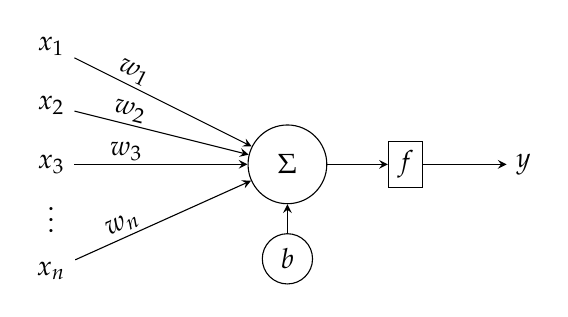
\begin{tikzpicture}[x=1.5cm, y=1.5cm]
    \node [] (input-1) at (0,0.5) {$x_1$};
    \node [] (input-2) at (0,0) {$x_2$};
    \node [] (input-3) at (0,-0.5) {$x_3$};
    \node [] (input-missing) at (0,-0.9) {$\vdots$};
    \node [] (input-n) at (0,-1.4) {$x_n$};

    \node [every neuron] (neuron) at (2,-0.5) {$\Sigma$};
    \node [bias] (bias) at (2,-1.3) {$b$};

    \node [activation] (act) at (3,-0.5) {$f$};
    \node [] (output) at (4,-0.5) {$y$};
    
    \foreach \i in {1,...,3,n}
    \draw [arrow] (input-\i) -- (neuron)
    node [above=-0.05, pos=0.3, sloped] {$w_\i$};

    \draw [arrow] (bias) -- (neuron);

    \draw [arrow] (neuron) -- (act);
    \draw [arrow] (act) -- (output);
  \end{tikzpicture}
  \caption{Artificial neuron.}
  \label{fig:neuron}
\end{figure}
An \ac{ann} is a model that performs elaboration in a way that
mimics the brain functioning. The base unit is the \ac{an}, also called
perceptron, of
\cref{fig:neuron}. It performs the weighted sum of the inputs
$x_1,\dots,x_n$, shifted by a bias $b$, followed by an activation
function $f$. If we add a dummy input $x_0=1$ and rename the bias
$b=w_0$, we can express the computation of the \ac{an} as in
\cref{eq:anComp}:
\begin{equation}\label{eq:anComp}
  y = f(\sum_{i=0}^n w_i x_i).
\end{equation}

The activation function $f$ can be of different types, the most common are:
\begin{itemize}
\item Softmax;
\item ReLU;
\item TanH;
\item Sigmoid;
\item Linear;
\end{itemize}

\begin{figure}
  \centering
  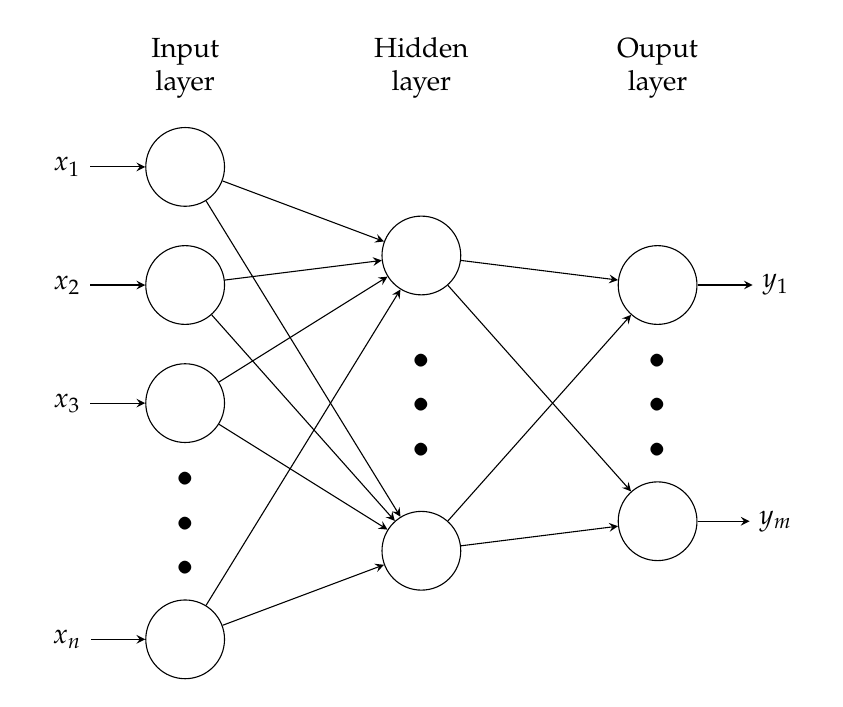
\begin{tikzpicture}[x=1.5cm, y=1.5cm]
    \foreach \m/\l [count=\y] in {1,2,3,missing,4}
    \node [every neuron/.try, neuron \m/.try] (input-\m) at (0,2.5-\y) {};

    \foreach \m [count=\y] in {1,missing,2}
    \node [every neuron/.try, neuron \m/.try ] (hidden-\m) at (2,2-\y*1.25) {};

    \foreach \m [count=\y] in {1,missing,2}
    \node [every neuron/.try, neuron \m/.try ] (output-\m) at (4,1.5-\y) {};

    \foreach \l [count=\i] in {1,2,3,n}
    \node[] (x-\i) at ($(input-\i)-(1,0)$) {$x_\l$};

    \foreach \l [count=\i] in {1,2,3,n}
    \draw [arrow] (x-\i) -- (input-\i);
    %\draw [arrowInverse] (input-\i) -- ++(-1,0)
    %node [above, midway] {$I_\l$};

    %\foreach \l [count=\i] in {1,n}
    %\node [above] at (hidden-\i.north) {$H_\l$};

    \foreach \l [count=\i] in {1,m}
    \node[] (y-\i) at ($(output-\i)+(1,0)$) {$y_\l$};
    
    \foreach \l [count=\i] in {1,n}
    \draw [arrow] (output-\i) -- (y-\i);
    %\draw [arrow] (output-\i) -- ++(1,0)
    %node [above, midway] {$O_\l$};

    \foreach \i in {1,...,4}
    \foreach \j in {1,...,2}
    \draw [arrow] (input-\i) -- (hidden-\j);

    \foreach \i in {1,...,2}
    \foreach \j in {1,...,2}
    \draw [arrow] (hidden-\i) -- (output-\j);

    \foreach \l [count=\x from 0] in {Input, Hidden, Ouput}
    \node [align=center, above] at (\x*2,2) {\l \\ layer};

  \end{tikzpicture}
  \caption{\acf{mlp} with one hidden layer.}
  \label{fig:ann}
\end{figure}
\acp{an} are organized in network structures. The basic layout of
an  \ac{ann} is the \acf{mlp} structured in layers like in
\cref{fig:ann}. Each \ac{an} of each layer is connected to all the
outputs of the previous layer. The first layer is connected to the
inputs of the \ac{ann} and the output of the last layer is also the
output of the network. The execution of the \ac{mlp} is feed forward:
\begin{enumerate}
\item the input values $x_{0,1},\dots x_{0,n}$ are presented to the
  network and it is the input of the first layer;
\item  the computation is 
  carried one layer at a time, where each neuron $i$ of the layer $l$
  calculates the value $y_{l,i}$ of the intermediate output
  $y_{l,1},\dots,y_{l,m}$;
\item the intermediate output $y_{l,1},\dots,y_{l,m}$ of the layer $l$
  becomes the 
  input $x_{l+1,1},\dots,x_{l+1,m}$ of the subsequent layer $l+1$,
  unless $l$ is the last layer - in that case the output of $l$ is the
  output $y_1,\dots,y_m$ of the \ac{mlp}.
\end{enumerate}

The weights of the \acp{an} are initialized to random values and, in order
to have meaningful outputs, the \ac{ann} needs to be trained. In a
supervised learning framework the dataset is composed of the matrices
$\matr{X}$ ($N\times n$) of the $N$ inputs $x_{i,j}$, and $\matr{Y}$
($N\times m$) of 
the corresponding outputs $y_{i,j}$. The
training process is called \emph{backpropagation} and it is organized in a
succession of phases. For each phase $p$ there are two steps:
\begin{description}
\item[execution] where an input $x_{p,1},\dots x_{p,n}$ is given to
  the network and an output $\hat{y}_{p,1},\dots,\hat{y}_{p,m}$ is calculated;
\item[weight update] where is calculated the error between
  $\hat{y}_{p,1},\dots,\hat{y}_{p,m}$ and the correct output
  $y_{p,1},\dots,y_{p,m}$, this error is back propagated through all
  the layers and a correction $\Delta w_i$ is calculated for each weight $w_i$ of
  the network, in
  order to minimize the error surface in the space of the weights.
\end{description}
In detail, to calculate the weights $\vect{w}^{(p+1)}$ for the next
phase $p+1$, it is 
sufficient to determine the gradient of 
the error surface in the current point $\vect{w}^{(t)}$ in order to
apply an optimization method like \ac{sgd}. We discuss \ac{sgd} in
detail in \cref{sec:sgd}.

\subsection{Loss}
The goal of the lerning algorithm is to learn a function $f$ such that
predictions $\hat{\vect{y}}=f(\vect{x})$ over the training set are accurate respect
to the correct labels $\vect{y}$. The \emph{loss} function quantifying
the prediction error. Formally a loss function
$\loss(\hat{\vect{y}},\vect{y})$ assign a scalar to a predicted output
given the true expected output, it should be lower bounded with the
minimum attained only for cases where the prediction is correct. The
parameters of the learned function, i.e. the weights $\vect{w}$, are
set in order to minimize the loss over the training examples. Given a
labeled training set $\mathcal{D}=(\vect{x}_{1:n},\vect{y}_{1:n})$ and a
parameterized model $f(\vect{x};\theta)$, the goal of the training
algorithm is then to set the values of the parameters $\theta$
such that the value of the loss is minimized:
\begin{equation}\label{eq:lossmin}
  \hat\theta=\argmin_\theta\frac{1}{n}\sum_{i=1}^n\loss(f(\vect{x}_i;\theta),\vect{y}_i).
\end{equation}

The parameters $\theta$ represents the set of all the weights $w$ of
the \ac{ann}. 
We proceed to describe common losses functions.

\subsubsection{Hinge loss}
Hinge loss, also known as margin loss is used in binary classification
problems, when the classifier output $\tilde{y}$ is a single scalar, and
$y\in\{+1,-1\}$. The classification rule is $\hat{y}=sign(\tilde{y})$
and the classification is considered correct if
$y\cdot\tilde{y}>0$. The hinge loss is defined as:
\begin{equation*}
  \loss_{hinge}(\tilde{y},y)=\max(0,1-y\cdot\tilde{y}).
\end{equation*}
It is $0$ when $\tilde{y}$ and $y$ share the same sign and
$|\tilde{y}|\geq 1$, otherwise the loss is linear. It attempts to
achieve a correct classification with a margin of at least 1.

Hinge loss can be also extended to multi-class settings, where
$\hat{\vect{y}}=\hat{y}_1,\dots,\hat{y}_n$ are the classifier's
output, and $\vect{y}$ the one-hot vector of correct output
classes. The classification rule is defined as selecting the class
with the highest score $\argmax_i\hat{\vect{y}}_i$. denoting by
$t=\argmax_iy_i$ the correct class index, and by $k=\argmax_{i\neq
  t}\hat{y}_i$ the highest scoring class such that $k\neq t$. The
multi-class hinge loss is defined as:
\begin{equation*}
  \loss_{hinge}(\hat{\vect{y}},
  \vect{y})=\max(0,1-(\hat{y}_t-\hat{y}_k)).
\end{equation*}
It attempts to score the correct class above all other classes with a
margin of at least 1.

\subsubsection{Log loss}
The log loss is a common variation of the hinge loss, it can be seen
as a soft version with an infinite margin \cite{lecun2006tutorial}. It
is defined as:
\begin{equation*}
  \loss_{log}(\hat{\vect{y}}, \vect{y}) =
  \log(1+\exp(-(\hat{\vect{y}}_t-\hat{\vect{y}}_k)). 
\end{equation*}

\subsubsection{Binary cross-entropy loss}
The binary cross-entropy loss, also called logistic loss, is used in
binary classification with conditional probability outputs. We have a
set of two target classes labeled with $y\in\{0,1\}$. The classifier's
output $\tilde{y}$ is transformed using the sigmoid (also logistic)
function $\sigma(x)=1/(1+e^{-x})$ to the range $[0,1]$. It can be
interpreted as the conditional probability
$\hat{y}=\sigma(\tilde{y})=\prob(y=1|\vect{x})$. The prediction rule is:
\begin{equation*}
  \begin{cases}
    0\quad\hat{y}<0.5,\\
    1\quad\hat{y}\geq 0.5.
  \end{cases}
\end{equation*}

The network is trained to maximize the log conditional probability for
each training example $(\vect{x},y)$. The logistic loss is defined as:
\begin{equation*}
  \loss_{logistic}(\hat{y},y)=-y\log\hat{y}-(1-y)\log(1-\hat{y}).
\end{equation*}

While the hinge loss is preferred when we require a hard decision
rule, the binary cross-entropy is useful when we want the network to
produce class conditional probability.

\subsubsection{Categorical cross-entropy loss}
The categorical cross-entropy, also called negative log likelihood, is
used when a probabilistic interpretation of the scores is desired. Let
$\vect{y}=y_1,\dots,y_n$ be a vector representing the true multinomial
distribution over the labels $1,\dots,n$, and let
$\hat{\vect{y}}=\hat{y}_1,\dots,\hat{y}_n$ be the classifier's output
transformed by a \emph{softmax} function:
\begin{equation*}
  softmax(\vect{x})_i=\frac{e^{x_i}}{\sum_j e^x_j}.
\end{equation*}
$\hat{\vect{y}}$ represent the class membership conditional
distribution $\hat{y}_i=\prob(y=i|\vect{x})$. The categorical cross
entropy loss measures the dissimilarity between the true label
distribution $\vect{y}$ and the predicted label distribution
$\hat{\vect{y}}$. It is defined:
\begin{equation*}
  \loss_{cross-entropy}(\hat{\vect{y}},\vect{y})=-\sum_i y_i\log(\hat{y}_i).
\end{equation*}

For hard classification problems in which each training example has a
single correct class assignment, $\vect{y}$ is the one-hot vector of
the true class. In such cases the cross-entropy loss can be simplified
to:
\begin{equation*}
  L_{cross-entropy}(\hat{\vect{y}},\vect{y}) = -\log(\hat{\vect{y}}_t),
\end{equation*}
where $t$ is the correct class.

\subsection{Regularization}
The attempt to minimize the loss with \eqref{eq:lossmin} may results 
in overfitting the training data, i.e. the model loose the capability
to generalize to new data, and the loss evaluates poorly on new data
that is not present in $\mathcal{D}$. To counter that, we often pose
soft restrictions on the form of the solution. This is done using a
\emph{regularization}
function $R(\theta)$ over the parameters returning a scalar that
reflect their \emph{complexity}. This is equivalent to introduce a
restriction over the hypothesis space as seen in
\cref{sec:supervisedTheory}. We want to keep the model complexity low,
thus we add the regularizer to \eqref{eq:lossmin} and we let the
optimization problem to balance between low loss and low complexity:
\begin{equation}\label{eq:lossminReg}
  \hat\theta=\argmin_\theta\left\{\frac{1}{n}\sum_{i=1}^n\loss(f(\vect{x}_i;\theta),\vect{y}_i)+\lambda
    R(\theta)\right\}.
\end{equation}

Different combinations of loss function and regularization criteria
result in different learning algorithms, with different inductive
biases.

In practice regularizers works penalizing high values for \ac{ann}
weights, thus avoiding that the network concentrates only on few
features. In \eqref{eq:lossminReg}, $R$ is applied to all the
parameters, in the practice it can be applied on the single layers.

We proceed to describe common regularization functions.

\subsubsection{$L_2$ regularization}
In $L_2$ regularization, also called \emph{gaussian prior} or
\emph{weight decay}, $R$ takes the form of the squared $L_2$ norm
of the parameters:
\begin{equation*}
  R_{L_2}(\matr{W})=||\matr{W}||_2^2=\sum_{i,j}(\matr{W}_{i,j})^2.
\end{equation*}

$L_2$ regularization penalizes high parameters, but when their values
becomes near to $0$ their effect is negligible.

\subsubsection{$L_1$ regularization}
In $L_1$ regularization, also called \emph{sparse prior} or
\emph{lasso}, $R$ takes the form of the $L_1$ norm of the parameters:
\begin{equation*}
  R_{L_1}(\matr{W})=||\matr{W}||_1=\sum_{i,j}|\matr{W}_{i,j}|.
\end{equation*}

In contrast to $L_2$, $L_1$ regularization penalizes uniformly low and
high parameters. This has the effect of encouraging a sparse solution
\cite{tibshirani1996regression}.

\subsubsection{Elastic-net}
The elastic-net regularizer \cite{zou2005regularization} combines both
$L_1$ and $L_2$ regularization:
\begin{equation*}
  R_{elastic-net}(\matr{W})=\lambda_1R_{L_1}(\matr{W})+\lambda_2R_{L_2}(\matr{W}).
\end{equation*}

\subsubsection{Dropout}
Similarly to other regularization techniques, \emph{dropout} method
\cite{hinton2012improving} is designed to prevent the network from
learning on specific weights. It works by randomly setting to $0$ the
output of a randomly chosen neurons for each sample. The connections
between the dropout technique and other regularizations are
established \cite{wager2013dropout}.
\subsection{\acf{sgd}}
\label{sec:sgd}
To successfully training a model, it is necessary to solve the
optimization problem \eqref{eq:lossmin}. A common solution is to use
gradient based methods. Gradient based methods works by estimating the
error computing the loss $\loss$ over the training set and then
calculating the 
gradients of the error respect to the parameters $\theta$. Once the
gradient is computed, the values of the weights are moved in the
opposite direction of the gradient. \acf{sgd} is a general
optimization algorithm that is profitably used in training \ac{ann}
\cite{bottou2012stochastic,lecun1995convolutional}.
\begin{algorithm}
  \caption{\acf{sgd}}\label{alg:sgd}
  \SetKwInput{Input}{Input}
  \Input{
    Parametrized function $f(\vect{x};\theta)$\\
    Training set $\mathcal{D}(\vect{x}_{1:n},\vect{y}_{1:n})$
  }
  \While{stopping criteria not met}{
    Sample training example $\vect{x}_i,\vect{y}_i$\;
    Compute $\loss(f(\vect{x}_i;\theta),\vect{y}_i)$\;
    $\hat{\vect{g}}\rightarrow$ gradients of
    $\loss(f(\vect{x}_i;\theta),\vect{y}_i)$ w.r.t. $\theta$\;
    $\theta\rightarrow\theta-\nu_t\hat{\vect{g}}$
  }
\end{algorithm}
The hyperparameter $\nu_t$ is the learning rate. It can be either
fixed throughout the learning process, or decay as a function of the
time step $t$. Adam is a widely used algorithm that adaptively change
the learning rate \cite{kingma2014adam}. The error calculated in
\cref{alg:sgd} is based on only one example. This may result in
inaccurate gradient calculation. A common way to reduce the noise of
this inaccuracy is to estimate the error and the gradients on a sample
of $m$ examples. This is called minibatch \ac{sgd}.

\subsection{\acf{rnn}}
\acp{rnn} are specialized versions of \ac{ann} for sequences. They
exhibit an
internal state $\vect{h}$ that changes during the training and that
recursively depends on the state of the previous phase. Precisely we
have \cref{eq:rnnState}:
\begin{equation}\label{eq:rnnState}
  \vect{h}^{(t)} = f(\vect{h}^{(t-1)}, \vect{x}^{(t)}; \vect{\theta}),
\end{equation}
where $\vect{h}$ is the state vector, $\vect{x}$ is the input vector
and $\vect{\theta}$ are the parameters of the state-function
$f$. The index $t$ indicates 
the iteration number, and can be interpreted as a discrete time or
more in general as the progressive number of the sequence that is
presented as
input.

\begin{figure}
  \centering
  % \subfigure[]{
  \subfloat[\label{fig:rnn1}]{
    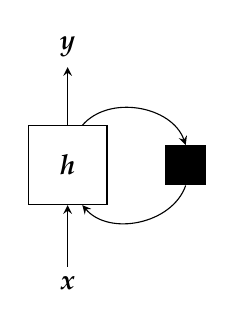
\begin{tikzpicture}[x=1.5cm, y=1.5cm]
      \node [] (input) at (0,0) {$\vect{x}$};

      \node [layer] (state) at (0,1) {$\vect{h}$};
      \node [delay] (delay) at (1,1) {};

      \node [] (output) at (0,2) {$\vect{y}$};
      
      \draw [arrow] (input) -- (state);
      \draw [arrow] (state) -- (output);
      \draw (state) edge[arrow, bend left=60] (delay.north);
      \draw (delay.south) edge[arrow, bend left=60] (state);
    \end{tikzpicture}
  }\hfill
  % \subfigure[]{
  \subfloat[\label{fig:rnn2}]{
    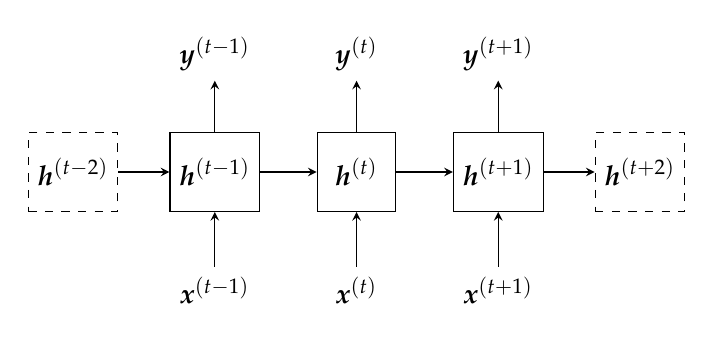
\begin{tikzpicture}[x=1.5cm, y=1.5cm]
      \foreach \l [count=\i] in {t-1,t,t+1}{
        \node [] (input-\i) at (\i*1.2,0) {$\vect{x}^{(\l)}$};
        \node [layer] (state-\i) at (\i*1.2,1) {$\vect{h}^{(\l)}$};
        \node [] (output-\i) at (\i*1.2,2) {$\vect{y}^{(\l)}$};

        \draw [arrow] (input-\i) -- (state-\i);
        \draw [arrow] (state-\i) -- (output-\i);
      }
      \node [layer, dashed] (state-l) at (0,1) {$\vect{h}^{(t-2)}$};
      \node [layer, dashed] (state-r) at (4*1.2,1) {$\vect{h}^{(t+2)}$};

      \draw [arrow] (state-l) -- (state-1);
      \draw [arrow] (state-1) -- (state-2);
      \draw [arrow] (state-2) -- (state-3);
      \draw [arrow] (state-3) -- (state-r);
    \end{tikzpicture}
  }
  \caption{\acf{rnn}, folded (a) and unfolded (b) models.}
  \label{fig:rnn}
\end{figure}
In order to express a compact visualisation of \acp{rnn} it is
possible to use the computational graph in \cref{fig:rnn1} where the
black box is a 
delay of one iteration. An extract of the unfolding of the computation
graph is 
shown in \cref{fig:rnn2}. 

\begin{figure}
  \centering
  \begin{tikzpicture}[x=1.5cm, y=1.5cm]
    \foreach \l [count=\i] in {t,t+1,missing,\tau}{
      \ifthenelse{\equal{\l}{missing}}{
        \node [vmissing] (state-\i) at (\i*1.2,1) {};
        \node [hmissing] (state-\i) at (\i*1.2,0) {};
      }{
        \node [] (input-\i) at (\i*1.2,0) {$\vect{x}^{(\l)}$};
        \node [layer] (state-\i) at (\i*1.2,1) {$\vect{h}^{(\l)}$};
        \draw [arrow] (input-\i) -- (state-\i);
        \ifthenelse{\equal{\l}{\tau}}{
          \node [] (output-\i) at (\i*1.2,2) {$\vect{y}^{(\l)}$};
          \draw [arrow] (state-\i) -- (output-\i);
        }
      }
    }

    \node [layer, dashed] (state-l) at (0,1) {$\vect{h}^{(t-1)}$};
    \node [layer, dashed] (state-r) at (5*1.2,1) {$\vect{h}^{(\tau+1)}$};

    \draw [arrow] (state-l) -- (state-1);
    \draw [arrow] (state-1) -- (state-2);
    \draw [arrow,dashed] (state-2) -- ++(0.8,0);
    \draw [arrowInverse,dashed] (state-4) -- ++(-0.8,0);
    \draw [arrow] (state-4) -- (state-r);
  \end{tikzpicture}
  \caption{\ac{rnn} with single output after a sequence of inputs.}
  \label{fig:rnnSO}
\end{figure}
The model in \cref{fig:rnn} provides an output $\vect{y}^{(t)}$ for every
input $\vect{x}^{(t)}$. An alternative is the model of
\cref{fig:rnnSO} where an output $\vect{y}^{(\tau)}$ is provided only
after a sequence $\vect{x}^{(t)},\dots,\vect{x}^{(\tau)}$ of inputs.

In order to train a \ac{rnn}, it is sufficient to apply the
backpropagation to the entire unfolded model.

\subsection{\acf{lstm}}
The major drawback of \acp{rnn} is the \emph{vanishing
  gradient} problem during the backpropagation. The gradient
for long-term associations, propagated through many stages, tends to
become zero. A possible solution for this problem is \ac{lstm} \cite{hochreiter1997long}.

\begin{figure}
  \centering
  % \subfigure[]{
  \subfloat[]{
    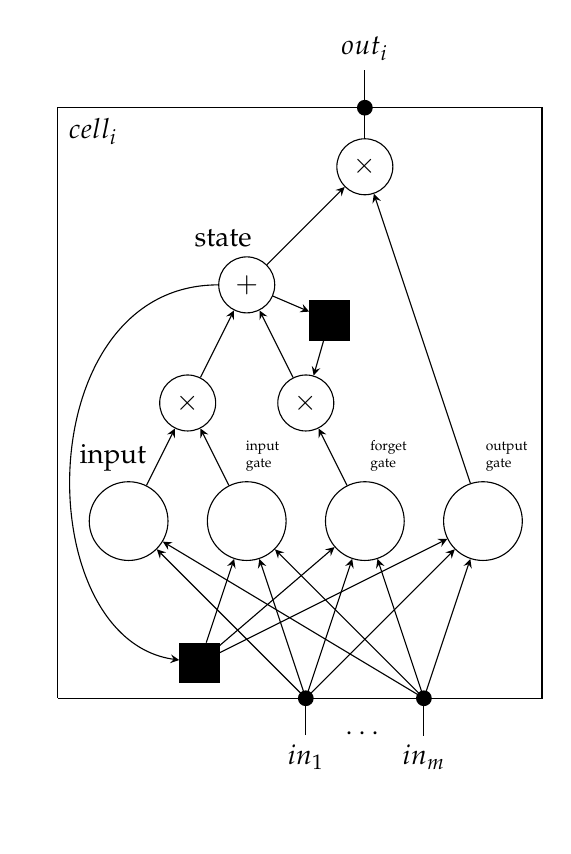
\begin{tikzpicture}[x=1.5cm, y=1.5cm]
      \node at (1,-0.5) {};

      \node[delay] (delay1) at (1.6,0.8) {};
      \coordinate (input1) at (2.5,0.5);
      \coordinate (input2) at (3.5,0.5);
      \node[] (input01) at (2.5,0) {$in_1$};
      \node[] (input02) at (3.5,0) {$in_m$};
      \node[] at (3,0.2) {$\cdots$};
      \node[every neuron, label={[xshift=-2mm]input}] (inputN) at (1,2) {};
      \node[every neuron, label={[xshift=2mm, align=left, font=\tiny] input\\gate}] (inputGate) at (2,2) {};
      \node[every neuron, label={[xshift=3mm, align=left, font=\tiny] forget\\gate}] (forgetGate) at (3,2) {};
      \node[every neuron, label={[xshift=3mm, align=left, font=\tiny] output\\gate}] (outputGate) at (4,2) {};
      \node[operation] (inputTimes) at (1.5, 3) {$\times$};
      \node[operation, label={[xshift=-3mm]state}] (state) at (2, 4) {$+$};
      \node[delay] (delay2) at (2.7,3.7) {};
      \node[operation] (forgetTimes) at (2.5, 3) {$\times$};
      \node[operation] (outputTimes) at (3, 5) {$\times$};
      \coordinate (output1) at (3,5.5);
      \node (output2) at (3,6) {$out_i$};
      \node at (0.7,5.3) {$cell_i$};

      \fill[black] (input1) circle (1mm);
      \fill[black] (input2) circle (1mm);
      \fill[black] (output1) circle (1mm);
      
      \foreach \n in {input1, input2}{
        \foreach \m in {inputN, inputGate, forgetGate, outputGate}{
          \draw[arrow] (\n) -- (\m);
        }
      }
      \foreach \m in {inputGate, forgetGate, outputGate}{
        \draw[arrow] (delay1) -- (\m);
      }

      \draw[arrow] (inputN) -- (inputTimes);
      \draw[arrow] (inputGate) -- (inputTimes);
      \draw[arrow] (forgetGate) -- (forgetTimes);
      \draw[arrow] (inputTimes) -- (state);
      \draw[arrow] (forgetTimes) -- (state);
      \draw [arrow] (state) ..  controls  (0.15,4) and (0.15,1) ..  (delay1);
      \draw[arrow] (state) -- (delay2);
      \draw[arrow] (delay2) -- (forgetTimes);
      \draw[arrow] (state) -- (outputTimes);
      \draw[arrow] (outputGate) -- (outputTimes);
      \draw[line] (outputTimes) -- (output1);
      \draw[line] (output1) -- (output2);
      \draw[line] (input01) -- (input1);
      \draw[line] (input02) -- (input2);

      \path[border] (0.4,0.5) -- (4.5,0.5) -- (4.5,5.5) -- (0.4,5.5) -- (0.4,0.5); 
      

    \end{tikzpicture}
    \label{fig:lstm1}
  }\hfill
  % \subfigure[]{
  \subfloat[]{
    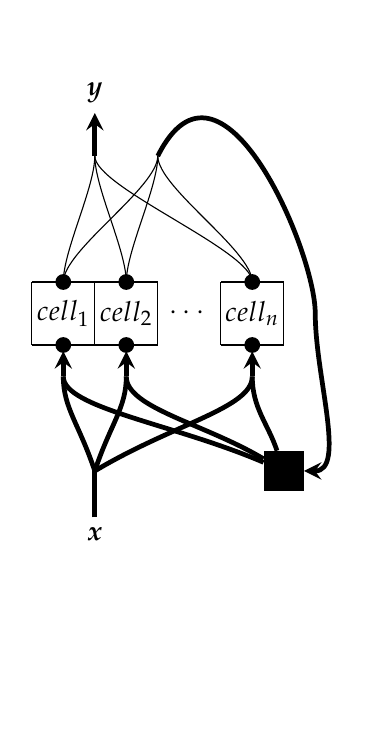
\begin{tikzpicture}[x=0.8cm, y=0.8cm]
      \node at (1,-2.5) {};

      % \draw[step=1.0,black,thin] (0,3) grid (4,4);
      \draw[step=1.0,black,thin] (0,3) grid (2,4);
      \draw[step=1.0,black,thin] (3,3) grid (4,4);
      \coordinate (input1) at (0.5,3);
      \coordinate (input2) at (1.5,3);
      \coordinate (input3) at (3.5,3);
      \coordinate (inputM1) at (0.5,2.5);
      \coordinate (inputM2) at (1.5,2.5);
      \coordinate (inputM3) at (3.5,2.5);
      \coordinate (output1) at (0.5,4);
      \coordinate (output2) at (1.5,4);
      \coordinate (output3) at (3.5,4);

      \coordinate (outputM) at (2,6);
      \coordinate (outputTM) at (1,6);
      
      \node at (0.5, 3.5) {$cell_1$};
      \node at (1.5, 3.5) {$cell_2$};
      \node at (2.5, 3.5) {$\cdots$};
      \node at (3.5, 3.5) {$cell_n$};
      \coordinate (pass) at (4.5, 3.5);
      \node (inputT) at (1,0) {$\vect{x}$};
      \coordinate (inputTM) at (1,1);
      \node (outputT) at (1,7) {$\vect{y}$};

      \node[delay] (delay) at (4,1) {};

      \foreach \c in {input1, input2, input3, output1, output2, output3}{
        \fill[black] (\c) circle (1mm);
      }

      \foreach \c in {inputM1, inputM2, inputM3}{
        \draw [vectorLine] (delay) ..  controls
        ($0.5*(delay)+0.5*(\c)$) and ($(\c)-(0,0.5)$) ..  (\c);
        \draw [vectorLine] (inputTM) ..  controls
        ($0.5*(inputTM)+0.5*(\c)$) and ($(\c)-(0,0.5)$) ..  (\c);
      }

      \foreach \c in {1, 2, 3}{
        \draw[vectorArrow] (inputM\c) -- ($(input\c)-(0,0.1)$);
      }

      \foreach \c in {output1, output2, output3}{
        \draw [line] (\c) ..  controls  ($(\c)+(0,0.5)$) and
        ($(outputM)-(0,0.5)$) ..  (outputM);
        \draw [line] (\c) ..  controls  ($(\c)+(0,0.5)$) and
        ($(outputTM)-(0,0.5)$) ..  (outputTM);
      }

      %\draw [vectorArrow] (outputM) ..  controls  ($(outputM)+(1,2)$) and ($(delay)+(1,0)$) ..  (delay);
      \draw [vectorArrow]
      (outputM) ..
      controls  ($(outputM)+(1,2)$) and ($(pass)+(0,1)$) ..
      (pass) ..
      controls  ($(pass)-(0,1)$) and ($(delay)+(1,0)$) ..
      (delay);
      \draw[vectorLine] (inputT) -- (inputTM);
      \draw[vectorArrow] (outputTM) -- (outputT);
    \end{tikzpicture}
    \label{fig:lstm2}
  }
  \caption{\ac{lstm} model: detail of memory cell (a), and general
    scheme (b). The black box is a delay of one iteration.}
  \label{fig:lstm}
\end{figure}
The \ac{lstm} model is structured as in \cref{fig:lstm}. It is
equivalent to a
generic \ac{rnn} where the hidden state $\vect{h}$ is a
layer of \emph{memory cells}.

In detail a single
memory cell (\cref{fig:lstm1}) has four \acf{an}. One is labelled \emph{input}
and processes the cell's 
inputs into an internal state. The other three \ac{an} are labelled as
\emph{gates} and process the cell's inputs together with the previous-phase
state in order to decide:
\begin{itemize}
\item how much of the current input must be learned
  (\emph{input gate});
\item how much of the previous-phase state must be forgotten
  (\emph{forget gate});
\item how much of the state constitutes the output (\emph{output gate}).
\end{itemize}

The memory-cells layer (\cref{fig:lstm2}) is composed of a number of
cells equal to the dimension of the output. Each cell
calculates one dimension of $\vect{y}$. The input $\vect{x}$ is copied
for every cell and, together with the previous-phase
output,
constitutes the input $in_1,\dots,in_m$ of the single cells.

\subsection{\acf{gru}}
The \ac{gru} was introduced by \cite{cho2014learning} as an
alternative to \ac{lstm}. \ac{gru} is also based on gating mechanism,
but it has fewer gates respect \ac{lstm} and the memory is directly
exposed to the output. One gate called \emph{reset} is used to control
access to the previous state and compute a proposed update. The new
status is calculated as an interpolation between the previous and the
proposed status, where the proportion of the interpolation is
controlled by the \emph{update} gate.

The choice between \ac{lstm} and \ac{gru} is context dependent, in
certain applications \ac{lstm} gives better performances, in other
applications \ac{gru} does \cite{yin2017comparative}. 




%%% Local Variables:
%%% mode: latex
%%% TeX-master: "thesis"
%%% End:

\chapter{Text analysis with deep learning}

\section{\ac{nlp}}
\ac{nlp} is the field of designing methods that take as input or
produce as output natural language data. Natural language is
ambiguous and variable, for instance the sentence ``i saw a woman on a
hill with a binocular'' can means that I had a binocular and with
those I saw a
woman on a hill, or that a woman was on a hill using the
binocular. This ambiguity can also be the source of problems in
specific context as the medical text, where specific countermeasures
can be adopted \cite{zhao_clinical_2019,codish2005model}.

Language is
\emph{symbolic} and \emph{discrete}, the relationship between different words,
i.e. symbols, can not be inferred from the symbols
themselves. It is possible to easily compare concepts that have a
continuous representation, e.g. two different colors in an image,
while it cannot be done easily with words without using large lookup
table or advanced methods. Language is also \emph{compositional},
letters form words, and words form sentences. Language is also
\emph{sparse}, the way in which words can be combined to form meanings
is practically infinite.

\section{\ac{ann} in \ac{nlp}}
\ac{ml} approaches are characterized by learning to make predictions
based on past observations. \ac{ann} approaches work by learning not
only to predict, but also to correctly represent data. A common
component of \ac{ann} applied to \ac{nlp} is the embedding layer,
i.e. a mapping from discrete symbols to continuous vectors in a
relatively low dimensional space. This representation allows to
transform the isolated symbols into mathematical objects that can be
operated on.

The principal model that is used in \ac{nlp} are \ac{rnn}. They are
capable of producing a vector that summarize the entire input
sequence. They allow abandoning the \emph{markov} assumption that was
prevalent in \ac{nlp} for decades, and designing models that can
condition on entire sentences or documents. This capability leads to
impressive gains in \emph{language-modeling}, the task of predicting
the probability of the next word in a sequence.

\subsection{Features}
The mapping from textual data to real valued vector that can be used
as input for \ac{ann} models, is called \emph{features extraction}.

When the focus entity is a word outside of a context, the main source
of information is the letters. We can look at \emph{lemma},
i.e. dictionary entry of the word, e.g. words such as ``booking'',
``booked'', ``books'' to their common lemma ``book''. This mapping is
usually performed using lemma lexicons or morphological analyzers. It
is a linguistically defined process and may not work well for forms
that are not in the lexicon or for mis-pelling. a coarser process is
called \emph{stemming}. A stemmer maps words to shorter words that are
not necessarily grammatically valid. E.g. ``picture'', ``pictures'',
and ``pictured'' will be stemmed to ``pictur''. \emph{Lexical
  resources} are dictionary that are meant to be accessed by machine
rather than by humans. They tipically contain information about words,
e.g. there are lexicons that map inflected word forms to their
possible morphological analyses, telling that a certain word may be a
singular masculine noun or a past-perfect verb.

When the focus entity is text, i.e. sentences, paragraphs documents,
the features are the count and the order of the letters and words
within the text. \emph{Bag of words} is a very common feature
extraction procedure. We look at the histogram of the words within the
text. We can also compute quantities that are directly derived from
the words and the letters such as the length of the sentence. We can
also integrate statistics based on external information. When using
bag of words, it is common to use \ac{tfidf} weighting
\cite{manning_introduction_2008}. A word $w$ in a document $d$ that is
part of a large corpus $D$ of documents is represented by:
\begin{equation*}
  \frac{\#_d(w)}{\sum_{w'\in d}\#_d(w')}\cdot\log\frac{|D|}{|d\in
    D:w\in d|},
\end{equation*}
where $\#_d(w)$ is the number of times that $w$ appears in
$d$. Besides words, one may also look at consecutive pairs or triplets
of words. These are called \emph{ngrams}. A bag of ngrams
representation is much more informative than a bag of words.

When considering a word within a sentence or a document, the features
of a word are its position within the sentence and the words or
letters surrounding it. It is common to focus on the immediate context
of a word by considering a \emph{window} surrounding it (with tipical
values of 2,5, and 10 words to each side). We may also be interested
in the absolute position of a word inside a sentence, having features
such as ``the word is the 5th in the sentence'' or ``the word appear
within the first 10 of the sentence''.

When considering more than a word within a context, we can also look
at the text \emph{distance} between them or the identities of the
words that appear between them.

Sentences in natural language have structures beyond the linear order
of their words. The structure is not directly observable and are
referred to as \emph{sintax}. While it is not observable it can be
inferred from the sentence. Specialized systems exist for the
prediction of parts of speech, syntactic trees, semantic roles,
discourse relations, and other linguistic properties. These prediction
often serve as good features for classification problems.

Different features can also be combined together. Instead of combining
them manually, we can provide a set of core features to an \ac{ann}
model and rely on the training procedure to pick up important
combinations of them.
Core features can also be learned by \ac{ann}, but enough data is
needed. The distributional hypothesis of language states that the
meaning of a word can be inferred from the contexts in which it is
used. By observing co-occurrence patterns of words across a large body
of text, it is possible to infer that a word is similar to another
word. Many algorithms were derived to make use of this property. They
can be categorized into clustering-based methods, with assign similar
words to the same cluster and represent each word by its cluster
membership \cite{miller2004name}, and embedding-based methods which
represent each word as a 
vector such that similar words (with similar distribution) have
similar vectors \cite{pennington_glove:_2014,mikolov_linguistic_2013}.

\section{Text classification}
\label{sec-baselines}
The classic approach is to employ bag-of-words
representations of textual documents
\cite{manning_introduction_2008}. In this approach, a document is 
described by a \textit{set} or a \textit{multiset} of words.
Multisets allow one to take into account the number of occurrences of
a word in the document. Vector representations of documents are easily
derived from bags-of-words. When using unigrams, the dimensionality of
each vector equals the size of the vocabulary in use. In the simplest
case, the vector $x$ representing a document has Boolean components
$x_j=1$ if and only if term $j$ appears in the document. A slightly more
informative representation, derived from multisets, is \ac{tfidf}
\cite{manning_introduction_2008}. In this case 
$x_j=n_j\log \frac{|D|}{|D_j|}$ where $n_j$ is the number of times
term $j$ occurs in the document, $|D|$ is the cardinality of the
data set, and $D_j$ is the set of documents containing term $j$. In
those representations, common terms receive a lower weight. An
alternative representation suggested in
\cite{martinez_information_2011} employed within-category frequencies
but only yielded modest improvements over \ac{tfidf} and thus we do not
use it in our baseline.

A more informative representation of documents can be obtained by
taking into account bigrams and trigrams, i.e.\ pairs or triplets or
terms that occur consecutively in a document. These representations
are suitable for large data sets and have been commonly employed in
other contexts.
% Explain how we used bigrams and trigrams

Bag-of-words representations (including those employing bigrams or
trigrams) enable the application of very simple text classifiers such
as \ac{nb} or \ac{svm} \cite{cortes-support-1995}. However, they
suffer two fundamental problems. First, the relative order of terms in
the documents is lost, making it impossible to take advantage of the
syntactic structure of the sentences. Second, distinct words have an
orthogonal representation even when they are semantically
close. Moreover the vast majority of the dataset, i.e. the unlabeled
records, remains unused with
this representation. As detailed in \cref{sec:word-vectors}, word
vectors can be used to address the seconf limitation and also allow us
to take advantage of unlabeled data, which can be typically be
obtained in large amounts and with little cost.

\section{Word Vectors}
\label{sec:word-vectors}
Many modern approaches to NLP take advantage of vector-space word
representations to solve specific tasks such as retrieval,
classification, named entity recognition or parsing. % Add citations
The use of word vectors eliminates the need for complex ontologies
like WordNet \cite{fellbaum-wordnet-1998}, that express various kinds of semantic relations among
words (such as synonymy, hypernymy, meronymy, etc). Word vectors are
typically constructed in such a way that analogies are directly
encoded in vector space. One often cited example of analogy is ``king
is to man as queen is to woman'', which should correspond to the
similarity in vector space~\cite{mikolov_linguistic_2013}:
$$
x_\mathit{king}-x_\mathit{man}+x_\mathit{woman} \approx x_\mathit{queen}.
$$
In a similar spirit, one could imagine the following vector space
similarity to occur in the oncology domain:
$$
x_\mathit{glioma}-x_\mathit{glia}+x_\mathit{connective} \approx
x_\mathit{fibroma}.
$$
\begin{figure}
  \centering
  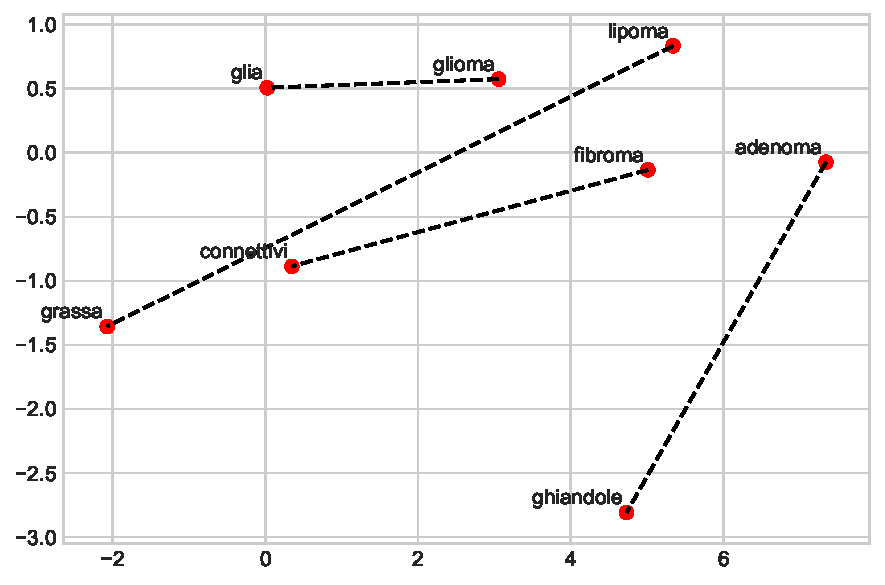
\includegraphics[width=0.5\textwidth]{img/gloveGraph.pdf}
  \caption{Extract from constructed vector space. The Italian labels
    are \emph{grassa} for \emph{fat}, \emph{connettivi} for
    \emph{connectives}, \emph{ghiandole} for \emph{glands}.}
  \label{fig:gloveGraph}
\end{figure}

Most algorithms for obtaining word vectors are based on co-occurrences
in large text corpora. Co-occurrence can be measured either at the
word-document level (e.g.\ using latent semantic analysis) or at the
word-word level (e.g.\ using word2vec~\cite{mikolov_linguistic_2013}
or \ac{glove}~\cite{pennington_glove:_2014}). It is a common practice to
take advantage of pre-compiled libraries of word vectors trained on
several billion tokens extracted from various sources such as
Wikipedia, the English Gigaword 5, Common Crawl, or Twitter. These
libraries are generally conceived for general purpose applications and
are only available for the English language. Since our cancer registry
textual data is written in Italian and employs a very specific domain
terminology, we retrained word vectors from the almost 1.5 millions
unlabeled records described in Section~\ref{sec:dataset}. For this
purpose, we trained \ac{glove}~\cite{pennington_glove:_2014}. An
excerpt of the trained dataset is visible in \cref{fig:gloveGraph}.

The training process involves the construction of the
$n\times n$ triangular matrix $C$ of words co-occurrence, where $n$ is
the number of unique words $w_1,\dots,w_n$ inside the text\footnote{Possibly excluded the
  most and the least frequent terms.}. In order to do this, a window of
size $\omega$ slides
through the text. After the construction of $C$, \ac{glove} uses the
information contained in it to train a model that produces vector of
specific dimension $\nu$.

$\omega$, $\nu$, and the number of
training iterations $\eta$ are parameters of the method. 

\section{\acs{bert}}
\ac{bert} \cite{devlin2018bert} is a recent model that represents the
state of the art in many \ac{nlp} related tasks
\cite{chatterjee2019semeval,hu2019introductory,lee2019biobert,tshitoyan2019unsupervised}.
It is a
bi-directional pre-training model backboned by the Transformer Encoder
\cite{vaswani2017attention}. It is an attention-based technique that
learns context-dependent word representation on large unlabeled
corpora, and then the model is fine tuned end to end on specific labeled
tasks. During pre-training, the model is trained
on unlabeled data over two different tasks. In \ac{mlm} some tokens
are masked and the model is trained to predict those token based on
the context. In \ac{nsp} the model is trained to understand the
relationship between sentences predicting if two sentences are actually
consecutive or if they where randomly replaced (with 50\%
probability). After the pre-training, the model is fine-tuned to the
specific task.

\section{Attention models}
Attention models are an important concept in neural networks that has
been researched within diverse application domains.

%%% Local Variables:
%%% mode: latex
%%% TeX-master: "thesis"
%%% End:

%\chapter{Background}
\label{ch:background}


%%% Local Variables:
%%% mode: latex
%%% TeX-master: "thesis"
%%% End:

\chapter{Materials and Methods}

\section{Dataset}
\label{sec:dataset}
We collected a set of $1\,592\,385$ anatomopathological exam results
from Tuscany region \ac{rtt} in the period 2004-2013. About $6\%$
of these records refer to a positive tumor
diagnosis and have topological and morphological ICD-O3 labels,
determined by tumor registry experts. Other reports are associated
with non-cancerous tissues and with unlabeled records. When multiple
pathological records for the
same patient existed for the same tumor, experts selected the most
informative report in order to assign the ICD-O3 code to that tumor
case, leaving a set of $94\,524$ labeled tumor cases.

Histological exam records consist of three free-text fields (not all
of them always filled-in), reporting tissue macroscopy, diagnosis,
and, in some cases, the patient's anamnesis. We found that field
semantics was not always used consistently and that the amount of
provided details varied significantly from extremely synthetic to very
detailed assessments of the morphology and the diagnosis. Field length
ranged from $0$ to $1\,368$ words, with first quartile, median and
third quartile respectively 34, 62, 134. For these reasons we merged
the three text fields
into a single text document, did not apply any conflation (except for
case normalization) kept punctuation.


In a second time, we further refined the dataset. We removed duplicate
reports and reports labeled with extremely rare (1048
samples that not
appear in either training, validation, and test sets) ICD-O3 codes. We
obtained in the end 
a dataset suitable for supervised learning consisting of $85\,170$
labeled records over $203$ morphological classes and $68$
topological classes.

We collected also the unlabeled rest of the dataset to train
unsupervised methods.

\subsection{Preparation}
The data used in this work comes from the \ac{rtt}. Originally it
comes in two tables. The first one is composed of
a list of
neoplasm records, for each one are specified: a series of
administrative variables, e.g.\ the date of incidence, the hospital;
\ac{icdo} codes, both first and third editions, for topography and
morphology; other clinical variables, e.g.\ \emph{Gleason},
\emph{Clark}, \emph{Dukes} scores.
\ac{icdo} codes inside neoplasm records are assigned by
\ac{rtt} personnel, thus they can be considered reliable and used as
ground truth for the learning models.

Furthermore, there is a histology table containing records resulting
from microscopy exams. Each record contains three free-text
fields, one for the macroscopy, one for the diagnosis, and one for
other information.
% Besides, the histology table contains \ac{icdo} and
% \ac{icdo3} codes resulting from the application of the preexisting
% rule-based classifier. We employ those codes in order to assess the
% existing
% system, and use it as a baseline.

The neoplasm and histology tables can be joined using a
neoplasm identifier. Thus connecting the text
fields with the true \ac{icdo} codes.

%The data set is composed of $309\,852$ neoplasm and $1\,592\,385$
%histology records. When joined, the resulting records are $94\,524$.

There are neoplasm cases
without a related histology exam because \ac{rtt} uses also other
sources to collect tumor cases, e.g.\ \acp{hdr} and death
certificates. There are also histology exams without a related
neoplasm 
case because not always a histology results in a tumor case.

To train the unsupervised methods, we keep all the records from the
histology table that cannot be joined with 
the neoplasm table.

\section{Models}\label{sec:models}
We realized in total seven models:
\begin{description}
\item[\svm] use \ac{svm} trained on \ac{tfidf} representations of text
  using unigrams;
\item[\svmb] use \ac{svm} trained on \ac{tfidf} representations
  using unigrams and bigrams;
\item[\lstmng] use \ac{lstm} layers trained on \ac{tfidf} representations using
  bigrams;
\item[\lstmc] use mixed convolutional and \ac{lstm} layers trained on
  \ac{glove} representations;
\item[\lstmb] use \ac{lstm} trained on \ac{glove} representations.
\item[\gru] use \ac{gru} layers trained on \ac{glove} representations.
\item[\maxp] use \ac{gru} layers with max pooling trained on \ac{glove}
  representations.
\item[\softmax] use \ac{gru} layers with attention trained on \ac{glove}
  representations.
\item[\maxi] use \ac{gru} layers with max pooling, in an interpretable setting, trained on \ac{glove}
  representations.
\item[\softmaxi] use \ac{gru} layers with attention, in an interpretable setting, trained on \ac{glove}
  representations.
\item[\maxh] use hierarchical \ac{gru} layers with max pooling trained on \ac{glove}
  representations.
\item[\softmaxh] use hierarchical \ac{gru} layers with attention trained on \ac{glove}
  representations.
\item[\bert] is the \ac{bert} model \cite{devlin2018bert} pretrained
  on our unlabeled data and fine tuned with our labeled data.
\end{description}

In models \svm{} and \svmb{} we used a \ac{tfidf}
representation ignoring terms present in less
than 3 documents or in
more than 30\% of the documents. 

We trained all the models except \ac{svm} minimizing
the \emph{categorical crossentropy}.

In \lstmng{} we used a word embedding of $30$. The
embedding layer corresponds to a one-hot representation of the input
followed by a dense layer of $30$ neurons.

\begin{figure}
  \centering
  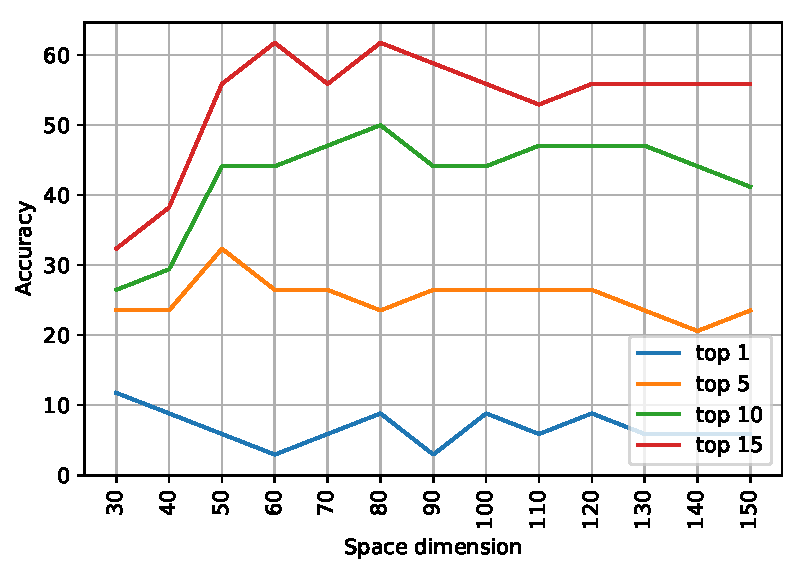
\includegraphics[width=0.45\textwidth]{img/gloveParameter.pdf}
  \caption{Accuracy top 1,5,10 and 15 for an intrinsic test with
    varying word vector dimension.}
  \label{fig:gloveParameter}
\end{figure}
In \lstmb{} and \lstmc{} we used the word vector representation
explained in \cref{sec:word-vectors}. We trained \ac{glove} with a window dimension of $15$,
in $50$ iterations to produce representations in dimension $60$. To
decide those parameters we developed intrinsic tests collecting
quadruples like:
$$
(melanoma,\ cute,\ duttale,\ mammella)
$$
translated:
$$
(melanoma,\ skin,\ ductal,\ breast)
$$
in order to verify if $\vect{x}_{breast}$ is near
$\vect{x}_{skin}-\vect{x}_{melanoma}+\vect{x}_{ductal}$. Then we
proceeded to confront the different parameters as in
\cref{fig:gloveParameter}.

In order to speed up the computation for the models \lstmng{}, \lstmb{}
and \lstmc{} we cut the length of text to 200. The
$87\%$ of records have less than 200 words.

\lstmng{} is the \ac{ann} in \cref{fig:schemeLstmng},
composed of two layers of $150$ bidirectional \ac{lstm} cells,
followed by an average pooling of the sequences, followed by a
dense \ac{relu} layer, followed by a dense \emph{softmax} layer.
The number of \acp{an} of the last two layers is
equal to the number of classes for each task.
\begin{figure}
  \centering
  \begin{tikzpicture}[node distance = 0.1cm, auto]
    \begin{scope}[start chain, every node/.style={on chain}, node distance = \schemeNodeDistance]
      \nodeInput();
      \nodeEmbedding();
      \node[support] (emb) {};
      \nodeLstm();
      \node[support] (lstmA) {};
      \nodeLstm();
      \node[support] (lstmB) {};
      \nodeAvg();
      \node[support] (avg) {};
      \nodeRelu();
      \node[support] (relu) {};
      \nodeSoftmax();
      \node[dataLabel, joined] {$outDim$};
    \end{scope}
    \node[dataLabel, above=of emb] {$200\times 30$};
    \node[dataLabel, above=of lstmA] {$200\times 300$};
    \node[dataLabel, above=of lstmB] {$200\times 300$};
    \node[dataLabel, above=of avg] {$300$};
    \node[dataLabel, above=of relu] {$outDim$};
  \end{tikzpicture}
  \caption{Scheme for \lstmng{} model.}
  \label{fig:schemeLstmng}
\end{figure}

\lstmc{}, in \cref{fig:schemeLstmc} is composed of a convolutional
filter of size two, followed by a bidirectional \ac{lstm} layer of
$150$ cells, followed by an average pooling of the sequences,
followed by a dense \ac{relu}, followed by a dense \emph{softmax}
layer.
\begin{figure}
  \centering
  \begin{tikzpicture}[node distance = 0.1cm, auto]
    \begin{scope}[start chain, every node/.style={on chain}, node distance = \schemeNodeDistance]
      \nodeInput();
      \nodeGlove();
      \node[support] (glove) {};
      \nodeConv();
      \node[support] (conv) {};
      \nodeLstm();
      \node[support] (lstm) {};
      \nodeAvg();
      \node[support] (avg) {};
      \nodeRelu();
      \node[support] (relu) {};
      \nodeSoftmax();
      \node[dataLabel, joined] {$outDim$};
    \end{scope}
    \node[dataLabel, above=of glove] {$200\times 60$};
    \node[dataLabel, above=of conv] {$199\times 100$};
    \node[dataLabel, above=of lstm] {$199\times 300$};
    \node[dataLabel, above=of avg] {$300$};
    \node[dataLabel, above=of relu] {$outDim$};
  \end{tikzpicture}
  \caption{Scheme for \lstmc{} model.}
  \label{fig:schemeLstmc}
\end{figure}

\lstmb{} in \cref{fig:schemeLstmb} is composed of two bidirectional
\ac{lstm} layer of 
$150$ cells, followed by an average pooling of the sequences,
followed by a dense \ac{relu}, followed by a dense \emph{softmax}
layer. 
\begin{figure}
  \centering
  \begin{tikzpicture}[node distance = 0.1cm, auto]
    \begin{scope}[start chain, every node/.style={on chain}, node distance = \schemeNodeDistance]
      \nodeInput();
      \nodeGlove();
      \node[support] (glove) {};
      \nodeLstm();
      \node[support] (lstmA) {};
      \nodeLstm();
      \node[support] (lstmB) {};
      \nodeAvg();
      \node[support] (avg) {};
      \nodeRelu();
      \node[support] (relu) {};
      \nodeSoftmax();
      \node[dataLabel, joined] {$outDim$};
    \end{scope}
    \node[dataLabel, above=of glove] {$200\times 60$};
    \node[dataLabel, above=of lstmA] {$200\times 300$};
    \node[dataLabel, above=of lstmB] {$200\times 300$};
    \node[dataLabel, above=of avg] {$300$};
    \node[dataLabel, above=of relu] {$outDim$};
  \end{tikzpicture}
  \caption{Scheme for \lstmb{} model.}
  \label{fig:schemeLstmb}
\end{figure}

\gru{} is a stacked bidirectional \ac{gru} model.

The other models where trained on different hyperparameters
configurations whose range is explained in
\cref{sec:hyperparameters}. We proceed to explain in detail their
structure.
\subsection{\maxp, \softmax, \maxi, \softmaxi}
\label{sec:model}
In our setting, a dataset $\mathcal{D}=\{(\vect{x}^{(i)},y^{(i)})\}$
consists of variable length sequence vectors $\vect{x}^{(i)}$, where
$x^{(i)}_t$, for $t=1,\dots,T^{(i)}$ is the $t$-th word in the $i$-th
document, and associated target classes
$y^{(i)}\in\{1,\dots,K\}$. Unless necessary, we will drop the
superscript in the following to keep notation simple.  Sequences will
be denoted in boldface. The RNN-based sequence classifiers used in
this work compute their predictions $f(\vect{x})$ as follows:
\begin{align}
  e_t &= E(x_t;\theta^e),\label{eq:embed}\\
  h^f_t &= F(e_t,h^f_{t-1};\theta^f),\label{eq:maxModelRL}\\  
  h^r_t &= R(e_t,h^r_{t+1};\theta^r),\label{eq:maxModelRR}\\
  u_t &= G(h_t;\theta^h),\label{eq:maxModelF}\\
  \phi &= A(\vect{h},\vect{u};\theta^a),\label{eq:aggregation}\\
  f(\vect{x}) &= g(\phi;\theta^c).\label{eq:maxModelC}
\end{align}
$E$ is an embedding function mapping words into $p$-dimensional real
vectors (where embedding parameters $\theta_e$ can be either
pretrained and adjustable or fixed, see Section~\ref{sec:word-vectors}
below.  Functions $F$ and $R$ corresponds to (forward and reverse)
dynamics that can be described in term of several (possibly layered)
recurrent cells. Each vector $h_t$,
the concatenation of $h^f_t$ and $h^r_t$, can be interpreted as latent
representations of the information contained at position $t$ in the
document. $G$ is an additional \ac{mlp} mapping each latent vector into a
vector $u_t$ that can be seen as contextualized representation of the
word at position $t$. $A$ is an aggregation function that creates a
single $d$-dimensional representation vector for the entire sequence
and $g$ is a softmax layer. Possible choices for the aggregator
function include:
\begin{itemize}
\item $\phi=(h^f_T,h^r_1)$, which just
  extract the extreme latent representations; these may be in
  principle sufficient since they depend on the whole sequence due to
  bidirectional dynamics; note however that this approach may require
  long-term dependencies to be effectively learned.
\item
  % $\phi = \sum_t a_t(\vect{u};\theta^a) h_t$,
  $\phi = \sum_t a_t(\vect{u};\theta^a) u_t$,
  using an attention mechanism as in~\cite{yang_hierarchical_2016}; in
  this case, (scalar) attention weights are computed as
  \begin{align*}
    c_t&=C(\vect{u};\theta^a),\\
    a_t(\vect{u};\theta^a) &= \frac{e^{\langle c, c_t\rangle}}
    {\sum_i{e^{\langle c, c_i\rangle}}},\\
  \end{align*}
  %$$
  %a_t(\vect{u};\theta^a) = \frac{e^{\langle \theta^a, u_t\rangle}}
  %{\sum_s{e^{\langle \theta^a, u_s\rangle}}}
  %$$
  where $C$ is a single layer that map the representation $u_t$ of the
  word to a hidden representation $c_t$, then the importance of the word is
  measured as a similarity with a context vector $c$ that is learned
  with the model and can be seen as an embedded representation of an
  high level query as in memory networks \cite{sukhbaatar2015end}.
\item $\phi = \max_t u_t$ where the maximum is taken element-wise
  along the sequence; this approach can be interpreted either as a
  simplified (parameter-less) attention mechanism or a bag-layer as
  proposed in the context of multi-instance
  learning~\cite{tibo2017network}; in this case each ``feature''
  $\phi_j$ will be positive if at least one of $u_{j,1},\dots,u_{j,T}$
  is positive; the resulting classifier will find it easy to create
  decision rules predicting a document as belonging to a certain class
  if a given set of contextualized word representations are present
  and another given set of contextualized word representations are
  absent in the sequence.
\end{itemize}

The parameters $\theta^f,\theta^r,\theta^h$ and $\theta^a$ (if
present) are determined by minimizing a loss function $\loss$
(categorical cross-entropy in our case) on training data:
\begin{equation}
  \hat \theta = \mathrm{arg}\min_\theta\sum_{(\vect{x},y)\in\mathcal{D}}\loss\left(y,f(\vect{x})\right),
\end{equation}
where $\theta=\theta^f\cup\theta^r\cup\theta^h\cup\theta^a$.

We call \maxp{} the model $f(\vect{x})$ when setting the aggregator
function $A$ equal to the max pooling $\max_t u_t$. When we use
instead the attention $\sum_t a_t(\vect{u};\theta^a) u_t$, we call the
model \softmax{}.

The model is flexible enough to gain interpretability under certain
assumptions. If we remove the last layer in \eqref{eq:maxModelC},
the dimension of last layer in \eqref{eq:maxModelF}
needs to be equal to the
output dimension (in the experiments: $1$ for the artificial dataset,
$68$ for the site task, and $203$ for the 
morphology).
We hypothesize that in this case, the values of
$u_t$ (or the weighted values $a_t(\vect{u};\sigma^a)u_t$ if we use the
attention as aggregator) collect information on the importance of the
area 
around $x_t$ for the purpose of classification task. This
information can be
used to interpret the model decision. We call \maxi{} this
interpretable setting when using the max aggregator, and \softmaxi{}
when using the attention.
% $e:\XSet\rightarrow\RSet^k$ is an embedding function that transforms
% sequence elements in tensors $\vect{x}_{i,j}=e(x_{i,j})$ of
% dimension $k$ that can be parsed by the
% model. $g:\YSet\rightarrow[0,1]^q$ is an embedding function that
% transforms sequences labels in one-hot encodings of a coherent
% dimension $q$.
\subsection{\maxh, \softmaxh}
\label{sec:modelh}
We extend the plain model of the previous section with a hierarchical setting,
similarly to other works \cite{yang_hierarchical_2016}. In this
setting our dataset $\mathcal{D}=\{\vect{x}^{(i)},y^{(i)}\}$
consists of variable length sequence of sequence vectors
$\vect{x}^{(i)}$, where $x_{s,t}^{(i)}$, for $s=1,\dots,S^{(i)}$ and
$t=1,\dots,T^{(i,s)}$ is the $t$-th word of the $s$-th sentence in the
$i$-th document, and associated target classes
$y^{(i)}\in\{1,\dots,K\}$. The prediction $f(\vect{x})$ is calculated:
\begin{align}
  e_{s,t} &= E(x_{s,t};\theta^e),\label{eq:embedH}\\
  h^f_{s,t} &= F(e_{s,t},h^f_{s,t-1};\theta^{f}),\label{eq:maxModelRLH}\\  
  h^r_{s,t} &= R(e_{s,t},h^r_{s,t+1};\theta^{r}),\label{eq:maxModelRRH}\\
  u_{s,t} &= G(h_{s,t};\theta^{h}),\label{eq:maxModelFH}\\
  \phi_s &= A(\vect{h}_s,\vect{u}_s;\theta^{a}),\label{eq:aggregationH}\\
  h'^{f}_{s} &= F'(\phi_{s},h'^{f}_{s-1};\theta'^{f}),\label{eq:maxModelRLHS}\\  
  h'^{r}_{s} &= R'(\phi_{s},h'^{r}_{s+1};\theta'^{r}),\label{eq:maxModelRRHS}\\
  \phi' &= A'(\vect{s},\vect{h}';\theta'^{a}),\label{eq:aggregationHS}\\
  f(\vect{x}) &= g(\phi';\theta^c).\label{eq:maxModelCH}
\end{align}
As in the plain model, $E$ is an embedding function, $F$ and $R$
corresponds to forward and reverse dynamics that process word
representations,
$h_{s,t}=h_{s,t}^f\oplus h_{s,t}^r$ is the latent representation of
the information contained at position $t$ of the $s$-th sentence,
$u_{s,t}$ is the contextualized representation of the word at position
$t$ of the $s$-th sentence, and $A$ is an aggregation function that
creates a single representation for the sentence. Furthermore $F'$ and
$R'$ corresponds to 
forward and reverse dynamics that process sentence representations,
and $A'$ is the aggregation function that creates a single
representation for the entire document. $h'_s=h'^f_s\oplus h'^r_s$
can be interpreted as the
latent representation of the information contained in the sentence $s$
for the document.

We call \maxh{} and \softmaxh{} the hierarchical model when we use
respectively the max pooling and the attention.


%%% Local Variables:
%%% mode: latex
%%% TeX-master: "thesis"
%%% End:

\chapter{Experiments}
With the experiments we want to show the feasibility of deep learning
methods and, more generally, machine learning methods applied to large
scale histological records. Moreover, we want to compare classical
bag-of-word techniques with recent deep learning methods. We also want
to assess the effects of leveraging large corpora of unlabeled text
that comes from the same distribution, in the context of text
classification. Finally, we want to check if attention-based methods
determine an improvement, especially when used in a hierarchic way
like in
previous works. We also want to show some practical use cases and
evaluate the interpretation of deep learning models.

In \cref{sec:metrics}, we describe some useful metrics that can
be used to assess the 
classifier behavior and also to use the classifiers in different use
cases.

In \cref{ch:icdoFirst}, we organize a comparative study between
\ac{svm} and deep learning techniques using both bag-of-words and word
vectors. We trained the models \svm, \svmb, \lstmng, \lstmc, and
\lstmb in 10-fold cross validation. We calculated 
different metrics for all the models and we summarized the average and
standard deviation 
along the folds. In these
experiments we can appreciate the improvements of using word
vectors. Furthermore, we can notice that by using \ac{svm}, either on
unigrams and bigrams, we already achieved good results.

Related to the motivations in \cref{sec:motivation}, with these
experiments we want to prove Q1. Also we want to answer to Q3 by
comparing ac{lstm} with
\ac{svm} with both \ac{glove} and bag-of-word features.  
With the training of word vectors we also want to answer to Q5.

In \ref{ch:artificial} we want to investigate the potentialities of
the attention based models and the simpler max aggregation. We
designed an artificial experiment where the two different
kinds of aggregation are compared. Moreover, we also used this artificial
dataset to preliminarily investigate the interpretability
potentialities of \maxi{} and \softmaxi{}. With these experiments we
want to show that the attention model is not always better than a
simpler max aggregation.

Regarding to the questions in \cref{sec:motivation}, these
artificial experiments are a preliminary answer to Q4 and Q6 because
we confront attention-based techniques with simpler aggregation
techniques. Also in these experiments we start to study the
interpretability of the models. 

In \cref{ch:icdo}, we changed the setting, instead of doing a 10-fold
cross validation we adopt a temporal split. This decision was made to
reflect a probable practical employment of the classifier, where it is
being trained on the past data and evaluated on future data. In these
experiments we are interested in evaluating the effects of the
attention models, comparing them with a simpler form constituted by
the max aggregation of \maxp{}. We focused on \ac{gru} because
preliminary experiments did not show an improvement of using
\ac{lstm}. With these experiments, we want to show that in this context
the adoption of hierarchical models is not beneficial. Moreover, we
want to evaluate how the interpretable models work respect to the
others.

Regarding the questions in \cref{sec:motivation}, these experiments
answer to Q1 (with different settings respect to the experiments in
\cref{ch:icdoFirst}). We answer to Q2 and Q4 because we apply attention and
hierarchical models to the cancer pathology reports. We also want to
answer to Q6 because we implement interpretable models. 


\section{Bag-of-words, word vectors, \ac{svm} and deep learning}
\label{ch:icdoFirst}
The focus of this section is to asses the improvement of employing
word vectors respect to the use of bag-of-words and to evaluate the
employment of deep learning techniques.

We realized four multiclass classifiers for the
histological exams. Calling $X$ the distribution of texts, $Y^s$
of site, $Y^f$ of full site (site plus subsite), $Y^t$ of type, and
$Y^b$ of behavior:
\begin{description}
  \item[\site{}] estimates $P(Y^s|X)$;
  \item[\fullSite{}] estimates $P(Y^f|X)$;
  \item[\type{}] estimates $P(Y^t|X)$;
  \item[\behaviour{}] estimates $P(Y^b|X)$.
\end{description}

% The different tasks are not fully independent: obviously \fullSite{}
% classification depends on \site{} classification, but also \type{},
% \behaviour{} and \site{} can be interdependent. Many types of tumor are
% associated to a specific site, some types even indicates a
% specific behavior. For instance, \type{} $8253$
% corresponds to the definition of \emph{bronchio-alveolar carcinoma,
%   mucinous}, and it can be only malignant (\behaviour{} $3$) and located in
% bronchus and lungs (\site{} $34$). Thus, some configurations are impossible.

% Every task is a multiclass classification problem because every
% record is assigned to a single couple of \ac{icdo} codes,
% topographical and morphological.

% We considered the third \ac{icdo} version. There are
% $94\,061$ records with \ac{icdo3} codes.
The tasks have a variable number of represented classes, summarized in
\cref{fig:numClasses}.
\begin{table}
  \center
  \caption{Number of classes for different tasks.}
  \label{fig:numClasses}
  \begin{tabular}{|l|c|}
    \hline
    task & classes \\
    \hline
    \site{} & 70 \\
    \fullSite{} & 284 \\
    \type{} & 434 \\
    \behaviour{} & 5 \\
    \hline
  \end{tabular}
\end{table}
Moreover, data is not balanced. As visible in \cref{fig:classDist},
some classes are common, while many are rare.
% In order to collect more than the
% $90\%$ of the 
% records it is sufficient to take the most frequent classes: $17$ over $70$
% for \site{}, $50$ over $284$ for \fullSite{},
% $44$ over $434$ for \type{}, and $2$ over $5$ for \behaviour{}
% classifications.
\begin{figure}
  \centering
  \includegraphics[width=0.45\textwidth]{img/classDist-icdo3-site.pdf}
  \includegraphics[width=0.45\textwidth]{img/classDist-icdo3-fullSite.pdf}
  \includegraphics[width=0.45\textwidth]{img/classDist-icdo3-type.pdf}
  \includegraphics[width=0.45\textwidth]{img/classDist-icdo3-behaviour.pdf}
  \caption{Documents in classes (ordered by
    frequency).}
  \label{fig:classDist}
\end{figure}

The frequency of words in the text
follows the typical Zipf's distribution with few words that cover the
majority of text and a long tail of infrequent words.
% The $85\%$ of
% the $9\,264\,143$ words in text is covered With $500$
% over a total of $35\,216$ distinct words. 


\subsection{Experiments}
\label{sec:experiments}
We used leave-one-out ten-folds cross validation
to take advantage of all the available data. The whole
pathological-record dataset was split in ten equal parts called
folds. To preserve labels distribution, this was performed in a
stratified way (all the folds have the same proportions of
labels). Afterwards, each
model was trained ten times, using one fold at a time as test
dataset and the remaining as training. For each metric we summarized the
average and the standard deviation among the runs. Regarding the
curves we calculated the cumulative for each 
one, i.e.\ we concatenated the prediction for all the folds and
calculated the curves on them. 

\begin{table}
  \centering
  \caption{Results for \site{} task.}
  \label{tab:resultsSite}
  %\scriptsize
  \footnotesize
  %\small
          \begin{tabular}{|l|l|r@{$\;\pm\;$}l|r@{$\;\pm\;$}l|r@{$\;\pm\;$}l|r@{$\;\pm\;$}l|r@{$\;\pm\;$}l|}
            \hline
            \multicolumn{2}{|c|}{} & \multicolumn{2}{c|}{\svm} & \multicolumn{2}{c|}{\svmb} & \multicolumn{2}{c|}{\lstmng} & \multicolumn{2}{c|}{\lstmc} & \multicolumn{2}{c|}{\lstmb}\\
            \hline
            \multicolumn{2}{|l|}{\textbf{accuracy}} & $89.8$ & $2.0$ & $89.8$ & $2.0$ & $88.6$ & $2.0$ & $90.0$ & $1.6$ & \underline{$90.5$} & $1.6$ \\
            \hline
            \multicolumn{2}{|l|}{\textbf{kappa}} & $88.5$ & $2.2$ & $88.6$ & $2.3$ & $87.2$ & $2.3$ & $88.9$ & $1.8$ & \underline{$89.3$} & $1.8$ \\
            \hline
            \multicolumn{2}{|l|}{\textbf{MAPs}} & $93.0$ & $1.5$ & $93.0$ & $1.5$ & $92.2$ & $1.5$ & $93.5$ & $1.2$ & \underline{$93.8$} & $1.1$ \\
            \hline
            \multicolumn{2}{|l|}{\textbf{MAPc}} & $61.6$ & $3.9$ & $61.3$ & $4.0$ & $55.7$ & $3.7$ & $62.7$ & $3.5$ & \underline{$64.1$} & $4.1$ \\
            \hline
            \multirow{2}{*}{\textbf{pre.}} & \textbf{ma.} & \underline{$65.5$} & $4.8$ & $64.7$ & $3.2$ & $55.0$ & $2.8$ & $61.5$ & $3.4$ & $61.8$ & $3.7$ \\
            \cline{2-12}& \textbf{we.} & $88.7$ & $2.0$ & $88.8$ & $2.0$ & $87.8$ & $1.8$ & $89.2$ & $1.6$ & \underline{$89.5$} & $1.7$ \\
            \hline
            \multirow{2}{*}{\textbf{rec.}} & \textbf{ma.} & $55.7$ & $4.1$ & $54.7$ & $3.8$ & $51.6$ & $3.2$ & $56.5$ & $3.0$ & \underline{$58.1$} & $3.5$ \\
            \cline{2-12}& \textbf{we.} & $89.8$ & $2.0$ & $89.8$ & $2.0$ & $88.6$ & $2.0$ & $90.0$ & $1.6$ & \underline{$90.5$} & $1.6$ \\
            \hline
            \multirow{2}{*}{\textbf{f1s.}} & \textbf{ma.} & \underline{$58.4$} & $4.1$ & $57.5$ & $3.6$ & $52.1$ & $3.1$ & $57.0$ & $2.7$ & $58.2$ & $3.3$ \\
            \cline{2-12}& \textbf{we.} & $88.9$ & $2.0$ & $89.0$ & $2.1$ & $88.0$ & $2.0$ & $89.3$ & $1.6$ & \underline{$89.7$} & $1.7$ \\
            \hline
        \end{tabular}

\end{table}

\begin{table}
  \centering
  \caption{Results for \fullSite{} task.}
  \label{tab:resultsFullSite}
  %\scriptsize
  \footnotesize
  %\small
          \begin{tabular}{|l|l|r@{$\;\pm\;$}l|r@{$\;\pm\;$}l|r@{$\;\pm\;$}l|r@{$\;\pm\;$}l|r@{$\;\pm\;$}l|}
            \hline
            \multicolumn{2}{|c|}{} & \multicolumn{2}{c|}{\svm} & \multicolumn{2}{c|}{\svmb} & \multicolumn{2}{c|}{\lstmng} & \multicolumn{2}{c|}{\lstmc} & \multicolumn{2}{c|}{\lstmb}\\
            \hline
            \multicolumn{2}{|l|}{\textbf{accuracy}} & $68.4$ & $2.3$ & $68.7$ & $2.0$ & $67.4$ & $1.7$ & $70.1$ & $2.1$ & \underline{$70.9$} & $2.0$ \\
            \hline
            \multicolumn{2}{|l|}{\textbf{kappa}} & $66.5$ & $2.4$ & $66.8$ & $2.1$ & $65.6$ & $1.7$ & $68.4$ & $2.2$ & \underline{$69.3$} & $2.1$ \\
            \hline
            \multicolumn{2}{|l|}{\textbf{MAPs}} & $78.4$ & $1.9$ & $78.4$ & $1.7$ & $78.5$ & $1.3$ & $80.6$ & $1.4$ & \underline{$81.3$} & $1.4$ \\
            \hline
            \multicolumn{2}{|l|}{\textbf{MAPc}} & $43.1$ & $2.2$ & $43.4$ & $2.2$ & $36.8$ & $2.3$ & $42.9$ & $2.6$ & \underline{$45.0$} & $2.0$ \\
            \hline
            \multirow{2}{*}{\textbf{pre.}} & \textbf{ma.} & $41.4$ & $1.6$ & \underline{$41.6$} & $1.5$ & $33.0$ & $2.8$ & $38.7$ & $3.1$ & $39.8$ & $2.3$ \\
            \cline{2-12}& \textbf{we.} & $66.3$ & $1.9$ & $67.1$ & $1.7$ & $66.1$ & $1.3$ & $68.8$ & $1.9$ & \underline{$69.5$} & $1.5$ \\
            \hline
            \multirow{2}{*}{\textbf{rec.}} & \textbf{ma.} & $35.7$ & $1.9$ & $35.1$ & $2.1$ & $32.0$ & $2.5$ & $36.6$ & $3.0$ & \underline{$38.0$} & $2.2$ \\
            \cline{2-12}& \textbf{we.} & $68.4$ & $2.3$ & $68.7$ & $2.0$ & $67.4$ & $1.7$ & $70.1$ & $2.1$ & \underline{$70.9$} & $2.0$ \\
            \hline
            \multirow{2}{*}{\textbf{f1s.}} & \textbf{ma.} & $36.6$ & $1.5$ & $36.4$ & $1.7$ & $31.2$ & $2.3$ & $35.9$ & $2.9$ & \underline{$37.3$} & $2.1$ \\
            \cline{2-12}& \textbf{we.} & $66.2$ & $2.1$ & $66.8$ & $1.8$ & $66.0$ & $1.3$ & $68.5$ & $2.0$ & \underline{$69.5$} & $1.8$ \\
            \hline
        \end{tabular}

\end{table}

\begin{table}
  \centering
  \caption{Results for \type{} task.}
  \label{tab:resultsType}
  %\scriptsize
  \footnotesize
  %\small
          \begin{tabular}{|l|l|r@{$\;\pm\;$}l|r@{$\;\pm\;$}l|r@{$\;\pm\;$}l|r@{$\;\pm\;$}l|r@{$\;\pm\;$}l|}
            \hline
            \multicolumn{2}{|c|}{} & \multicolumn{2}{c|}{\svm} & \multicolumn{2}{c|}{\svmb} & \multicolumn{2}{c|}{\lstmng} & \multicolumn{2}{c|}{\lstmc} & \multicolumn{2}{c|}{\lstmb}\\
            \hline
            \multicolumn{2}{|l|}{\textbf{accuracy}} & $81.9$ & $1.9$ & $82.9$ & $2.0$ & $82.8$ & $1.4$ & $84.6$ & $1.4$ & \underline{$84.9$} & $1.5$ \\
            \hline
            \multicolumn{2}{|l|}{\textbf{kappa}} & $79.5$ & $2.2$ & $80.7$ & $2.3$ & $80.6$ & $1.6$ & $82.7$ & $1.6$ & \underline{$83.0$} & $1.7$ \\
            \hline
            \multicolumn{2}{|l|}{\textbf{MAPs}} & $87.8$ & $1.3$ & $88.6$ & $1.4$ & $88.7$ & $1.0$ & $90.3$ & $0.9$ & \underline{$90.6$} & $1.0$ \\
            \hline
            \multicolumn{2}{|l|}{\textbf{MAPc}} & $62.4$ & $1.6$ & $64.4$ & $1.8$ & $55.1$ & $3.1$ & $64.2$ & $1.9$ & \underline{$65.9$} & $1.9$ \\
            \hline
            \multirow{2}{*}{\textbf{pre.}} & \textbf{ma.} & $56.1$ & $2.4$ & \underline{$58.3$} & $1.9$ & $47.0$ & $3.3$ & $56.5$ & $1.8$ & $57.0$ & $2.6$ \\
            \cline{2-12}& \textbf{we.} & $80.3$ & $1.8$ & $81.8$ & $1.9$ & $82.0$ & $1.3$ & $84.1$ & $1.3$ & \underline{$84.3$} & $1.5$ \\
            \hline
            \multirow{2}{*}{\textbf{rec.}} & \textbf{ma.} & $51.1$ & $2.6$ & $52.2$ & $2.2$ & $47.0$ & $2.6$ & $56.8$ & $2.2$ & \underline{$58.6$} & $2.0$ \\
            \cline{2-12}& \textbf{we.} & $81.9$ & $1.9$ & $82.9$ & $2.0$ & $82.8$ & $1.4$ & $84.6$ & $1.4$ & \underline{$84.9$} & $1.5$ \\
            \hline
            \multirow{2}{*}{\textbf{f1s.}} & \textbf{ma.} & $51.4$ & $2.5$ & $52.9$ & $1.9$ & $45.0$ & $2.9$ & $54.6$ & $1.9$ & \underline{$55.5$} & $2.3$ \\
            \cline{2-12}& \textbf{we.} & $80.4$ & $2.0$ & $81.7$ & $2.0$ & $81.9$ & $1.3$ & $83.8$ & $1.4$ & \underline{$84.0$} & $1.5$ \\
            \hline
        \end{tabular}

\end{table}

\begin{table}
  \centering
  \caption{Results for \behaviour{} task.}
  \label{tab:resultsBehaviour}
  %\scriptsize
  \footnotesize
  %\small
          \begin{tabular}{|l|l|r@{$\;\pm\;$}l|r@{$\;\pm\;$}l|r@{$\;\pm\;$}l|r@{$\;\pm\;$}l|r@{$\;\pm\;$}l|}
            \hline
            \multicolumn{2}{|c|}{} & \multicolumn{2}{c|}{\svm} & \multicolumn{2}{c|}{\svmb} & \multicolumn{2}{c|}{\lstmng} & \multicolumn{2}{c|}{\lstmc} & \multicolumn{2}{c|}{\lstmb}\\
            \hline
            \multicolumn{2}{|l|}{\textbf{accuracy}} & $95.9$ & $1.0$ & $96.0$ & $1.1$ & $94.1$ & $3.0$ & $94.4$ & $4.2$ & \underline{$96.5$} & $0.8$ \\
            \hline
            \multicolumn{2}{|l|}{\textbf{kappa}} & $82.3$ & $4.6$ & $82.8$ & $5.0$ & $70.4$ & $25.5$ & $67.6$ & $35.9$ & \underline{$85.6$} & $3.4$ \\
            \hline
            \multicolumn{2}{|l|}{\textbf{MAPs}} & $97.7$ & $0.6$ & $97.8$ & $0.6$ & $96.6$ & $1.8$ & $96.8$ & $2.5$ & \underline{$98.1$} & $0.5$ \\
            \hline
            \multicolumn{2}{|l|}{\textbf{MAPc}} & $85.4$ & $5.9$ & $85.9$ & $5.7$ & $71.4$ & $18.4$ & $75.5$ & $26.4$ & \underline{$89.5$} & $4.2$ \\
            \hline
            \multirow{2}{*}{\textbf{pre.}} & \textbf{ma.} & $87.0$ & $5.0$ & \underline{$87.9$} & $4.8$ & $69.9$ & $19.9$ & $72.7$ & $27.1$ & $85.5$ & $4.0$ \\
            \cline{2-12}& \textbf{we.} & $95.8$ & $1.1$ & $95.9$ & $1.2$ & $92.6$ & $6.4$ & $92.1$ & $9.0$ & \underline{$96.6$} & $0.8$ \\
            \hline
            \multirow{2}{*}{\textbf{rec.}} & \textbf{ma.} & $78.6$ & $7.3$ & $78.6$ & $7.4$ & $67.6$ & $17.4$ & $72.1$ & $25.4$ & \underline{$85.9$} & $4.9$ \\
            \cline{2-12}& \textbf{we.} & $95.9$ & $1.0$ & $96.0$ & $1.1$ & $94.1$ & $3.0$ & $94.4$ & $4.2$ & \underline{$96.5$} & $0.8$ \\
            \hline
            \multirow{2}{*}{\textbf{f1s.}} & \textbf{ma.} & $81.7$ & $6.3$ & $82.0$ & $6.3$ & $68.0$ & $18.5$ & $72.1$ & $26.0$ & \underline{$85.5$} & $4.2$ \\
            \cline{2-12}& \textbf{we.} & $95.8$ & $1.1$ & $95.9$ & $1.2$ & $93.2$ & $4.8$ & $93.1$ & $6.7$ & \underline{$96.5$} & $0.8$ \\
            \hline
        \end{tabular}

\end{table}

The results are summarized in
\cref{tab:resultsSite,tab:resultsFullSite,tab:resultsType,tab:resultsBehaviour},
one table for each task, one column for each 
model described in \cref{sec:models}. Rows specify the metrics
described in \cref{sec:metrics}, with also macro and weighted average
for precision, recall and $F_1$ score. Micro averages are not
visualized because equivalent to accuracy. Values are expressed in
percentage, indicating average and standard deviation among folds.
%, furthermore for the model \lstmb{} we added another
%task: \emph{full site stacked}. Such task is to classify the \emph{full site}
%having already the \emph{site} code assigned.

\begin{figure}
  \centering
  \resizebox{0.9\textwidth}{!}{%% Creator: Matplotlib, PGF backend
%%
%% To include the figure in your LaTeX document, write
%%   \input{<filename>.pgf}
%%
%% Make sure the required packages are loaded in your preamble
%%   \usepackage{pgf}
%%
%% Figures using additional raster images can only be included by \input if
%% they are in the same directory as the main LaTeX file. For loading figures
%% from other directories you can use the `import` package
%%   \usepackage{import}
%% and then include the figures with
%%   \import{<path to file>}{<filename>.pgf}
%%
%% Matplotlib used the following preamble
%%   \newcommand{\svm}{xxxxxxxxxx}
%%   \newcommand{\svmb}{xxxxxxxxxx}
%%   \newcommand{\lstmng}{xxxxxxxxxx}
%%   \newcommand{\lstmc}{xxxxxxxxxx}
%%   \newcommand{\lstmb}{xxxxxxxxxx}
%%   \newcommand{\site}{xxxxxxxxxx}
%%   \newcommand{\fullSite}{xxxxxxxxxx}
%%   \newcommand{\type}{xxxxxxxxxx}
%%   \newcommand{\behaviour}{xxxxxxxxxx}
%%   \usepackage{fontspec}
%%
\begingroup%
\makeatletter%
\begin{pgfpicture}%
\pgfpathrectangle{\pgfpointorigin}{\pgfqpoint{5.392361in}{3.827777in}}%
\pgfusepath{use as bounding box, clip}%
\begin{pgfscope}%
\pgfsetbuttcap%
\pgfsetmiterjoin%
\definecolor{currentfill}{rgb}{1.000000,1.000000,1.000000}%
\pgfsetfillcolor{currentfill}%
\pgfsetlinewidth{0.000000pt}%
\definecolor{currentstroke}{rgb}{1.000000,1.000000,1.000000}%
\pgfsetstrokecolor{currentstroke}%
\pgfsetdash{}{0pt}%
\pgfpathmoveto{\pgfqpoint{0.000000in}{0.000000in}}%
\pgfpathlineto{\pgfqpoint{5.392361in}{0.000000in}}%
\pgfpathlineto{\pgfqpoint{5.392361in}{3.827777in}}%
\pgfpathlineto{\pgfqpoint{0.000000in}{3.827777in}}%
\pgfpathclose%
\pgfusepath{fill}%
\end{pgfscope}%
\begin{pgfscope}%
\pgfsetbuttcap%
\pgfsetmiterjoin%
\definecolor{currentfill}{rgb}{1.000000,1.000000,1.000000}%
\pgfsetfillcolor{currentfill}%
\pgfsetlinewidth{0.000000pt}%
\definecolor{currentstroke}{rgb}{0.000000,0.000000,0.000000}%
\pgfsetstrokecolor{currentstroke}%
\pgfsetstrokeopacity{0.000000}%
\pgfsetdash{}{0pt}%
\pgfpathmoveto{\pgfqpoint{0.553611in}{0.499444in}}%
\pgfpathlineto{\pgfqpoint{5.203611in}{0.499444in}}%
\pgfpathlineto{\pgfqpoint{5.203611in}{3.519444in}}%
\pgfpathlineto{\pgfqpoint{0.553611in}{3.519444in}}%
\pgfpathclose%
\pgfusepath{fill}%
\end{pgfscope}%
\begin{pgfscope}%
\pgfsetbuttcap%
\pgfsetroundjoin%
\definecolor{currentfill}{rgb}{0.000000,0.000000,0.000000}%
\pgfsetfillcolor{currentfill}%
\pgfsetlinewidth{0.803000pt}%
\definecolor{currentstroke}{rgb}{0.000000,0.000000,0.000000}%
\pgfsetstrokecolor{currentstroke}%
\pgfsetdash{}{0pt}%
\pgfsys@defobject{currentmarker}{\pgfqpoint{0.000000in}{-0.048611in}}{\pgfqpoint{0.000000in}{0.000000in}}{%
\pgfpathmoveto{\pgfqpoint{0.000000in}{0.000000in}}%
\pgfpathlineto{\pgfqpoint{0.000000in}{-0.048611in}}%
\pgfusepath{stroke,fill}%
}%
\begin{pgfscope}%
\pgfsys@transformshift{0.553611in}{0.499444in}%
\pgfsys@useobject{currentmarker}{}%
\end{pgfscope}%
\end{pgfscope}%
\begin{pgfscope}%
\pgftext[x=0.553611in,y=0.402222in,,top]{\sffamily\fontsize{10.000000}{12.000000}\selectfont 0.0}%
\end{pgfscope}%
\begin{pgfscope}%
\pgfsetbuttcap%
\pgfsetroundjoin%
\definecolor{currentfill}{rgb}{0.000000,0.000000,0.000000}%
\pgfsetfillcolor{currentfill}%
\pgfsetlinewidth{0.803000pt}%
\definecolor{currentstroke}{rgb}{0.000000,0.000000,0.000000}%
\pgfsetstrokecolor{currentstroke}%
\pgfsetdash{}{0pt}%
\pgfsys@defobject{currentmarker}{\pgfqpoint{0.000000in}{-0.048611in}}{\pgfqpoint{0.000000in}{0.000000in}}{%
\pgfpathmoveto{\pgfqpoint{0.000000in}{0.000000in}}%
\pgfpathlineto{\pgfqpoint{0.000000in}{-0.048611in}}%
\pgfusepath{stroke,fill}%
}%
\begin{pgfscope}%
\pgfsys@transformshift{1.483611in}{0.499444in}%
\pgfsys@useobject{currentmarker}{}%
\end{pgfscope}%
\end{pgfscope}%
\begin{pgfscope}%
\pgftext[x=1.483611in,y=0.402222in,,top]{\sffamily\fontsize{10.000000}{12.000000}\selectfont 0.2}%
\end{pgfscope}%
\begin{pgfscope}%
\pgfsetbuttcap%
\pgfsetroundjoin%
\definecolor{currentfill}{rgb}{0.000000,0.000000,0.000000}%
\pgfsetfillcolor{currentfill}%
\pgfsetlinewidth{0.803000pt}%
\definecolor{currentstroke}{rgb}{0.000000,0.000000,0.000000}%
\pgfsetstrokecolor{currentstroke}%
\pgfsetdash{}{0pt}%
\pgfsys@defobject{currentmarker}{\pgfqpoint{0.000000in}{-0.048611in}}{\pgfqpoint{0.000000in}{0.000000in}}{%
\pgfpathmoveto{\pgfqpoint{0.000000in}{0.000000in}}%
\pgfpathlineto{\pgfqpoint{0.000000in}{-0.048611in}}%
\pgfusepath{stroke,fill}%
}%
\begin{pgfscope}%
\pgfsys@transformshift{2.413611in}{0.499444in}%
\pgfsys@useobject{currentmarker}{}%
\end{pgfscope}%
\end{pgfscope}%
\begin{pgfscope}%
\pgftext[x=2.413611in,y=0.402222in,,top]{\sffamily\fontsize{10.000000}{12.000000}\selectfont 0.4}%
\end{pgfscope}%
\begin{pgfscope}%
\pgfsetbuttcap%
\pgfsetroundjoin%
\definecolor{currentfill}{rgb}{0.000000,0.000000,0.000000}%
\pgfsetfillcolor{currentfill}%
\pgfsetlinewidth{0.803000pt}%
\definecolor{currentstroke}{rgb}{0.000000,0.000000,0.000000}%
\pgfsetstrokecolor{currentstroke}%
\pgfsetdash{}{0pt}%
\pgfsys@defobject{currentmarker}{\pgfqpoint{0.000000in}{-0.048611in}}{\pgfqpoint{0.000000in}{0.000000in}}{%
\pgfpathmoveto{\pgfqpoint{0.000000in}{0.000000in}}%
\pgfpathlineto{\pgfqpoint{0.000000in}{-0.048611in}}%
\pgfusepath{stroke,fill}%
}%
\begin{pgfscope}%
\pgfsys@transformshift{3.343611in}{0.499444in}%
\pgfsys@useobject{currentmarker}{}%
\end{pgfscope}%
\end{pgfscope}%
\begin{pgfscope}%
\pgftext[x=3.343611in,y=0.402222in,,top]{\sffamily\fontsize{10.000000}{12.000000}\selectfont 0.6}%
\end{pgfscope}%
\begin{pgfscope}%
\pgfsetbuttcap%
\pgfsetroundjoin%
\definecolor{currentfill}{rgb}{0.000000,0.000000,0.000000}%
\pgfsetfillcolor{currentfill}%
\pgfsetlinewidth{0.803000pt}%
\definecolor{currentstroke}{rgb}{0.000000,0.000000,0.000000}%
\pgfsetstrokecolor{currentstroke}%
\pgfsetdash{}{0pt}%
\pgfsys@defobject{currentmarker}{\pgfqpoint{0.000000in}{-0.048611in}}{\pgfqpoint{0.000000in}{0.000000in}}{%
\pgfpathmoveto{\pgfqpoint{0.000000in}{0.000000in}}%
\pgfpathlineto{\pgfqpoint{0.000000in}{-0.048611in}}%
\pgfusepath{stroke,fill}%
}%
\begin{pgfscope}%
\pgfsys@transformshift{4.273611in}{0.499444in}%
\pgfsys@useobject{currentmarker}{}%
\end{pgfscope}%
\end{pgfscope}%
\begin{pgfscope}%
\pgftext[x=4.273611in,y=0.402222in,,top]{\sffamily\fontsize{10.000000}{12.000000}\selectfont 0.8}%
\end{pgfscope}%
\begin{pgfscope}%
\pgfsetbuttcap%
\pgfsetroundjoin%
\definecolor{currentfill}{rgb}{0.000000,0.000000,0.000000}%
\pgfsetfillcolor{currentfill}%
\pgfsetlinewidth{0.803000pt}%
\definecolor{currentstroke}{rgb}{0.000000,0.000000,0.000000}%
\pgfsetstrokecolor{currentstroke}%
\pgfsetdash{}{0pt}%
\pgfsys@defobject{currentmarker}{\pgfqpoint{0.000000in}{-0.048611in}}{\pgfqpoint{0.000000in}{0.000000in}}{%
\pgfpathmoveto{\pgfqpoint{0.000000in}{0.000000in}}%
\pgfpathlineto{\pgfqpoint{0.000000in}{-0.048611in}}%
\pgfusepath{stroke,fill}%
}%
\begin{pgfscope}%
\pgfsys@transformshift{5.203611in}{0.499444in}%
\pgfsys@useobject{currentmarker}{}%
\end{pgfscope}%
\end{pgfscope}%
\begin{pgfscope}%
\pgftext[x=5.203611in,y=0.402222in,,top]{\sffamily\fontsize{10.000000}{12.000000}\selectfont 1.0}%
\end{pgfscope}%
\begin{pgfscope}%
\pgftext[x=2.878611in,y=0.223333in,,top]{\sffamily\fontsize{10.000000}{12.000000}\selectfont Recall}%
\end{pgfscope}%
\begin{pgfscope}%
\pgfsetbuttcap%
\pgfsetroundjoin%
\definecolor{currentfill}{rgb}{0.000000,0.000000,0.000000}%
\pgfsetfillcolor{currentfill}%
\pgfsetlinewidth{0.803000pt}%
\definecolor{currentstroke}{rgb}{0.000000,0.000000,0.000000}%
\pgfsetstrokecolor{currentstroke}%
\pgfsetdash{}{0pt}%
\pgfsys@defobject{currentmarker}{\pgfqpoint{-0.048611in}{0.000000in}}{\pgfqpoint{0.000000in}{0.000000in}}{%
\pgfpathmoveto{\pgfqpoint{0.000000in}{0.000000in}}%
\pgfpathlineto{\pgfqpoint{-0.048611in}{0.000000in}}%
\pgfusepath{stroke,fill}%
}%
\begin{pgfscope}%
\pgfsys@transformshift{0.553611in}{0.499444in}%
\pgfsys@useobject{currentmarker}{}%
\end{pgfscope}%
\end{pgfscope}%
\begin{pgfscope}%
\pgftext[x=0.278889in,y=0.451250in,left,base]{\sffamily\fontsize{10.000000}{12.000000}\selectfont 0.0}%
\end{pgfscope}%
\begin{pgfscope}%
\pgfsetbuttcap%
\pgfsetroundjoin%
\definecolor{currentfill}{rgb}{0.000000,0.000000,0.000000}%
\pgfsetfillcolor{currentfill}%
\pgfsetlinewidth{0.803000pt}%
\definecolor{currentstroke}{rgb}{0.000000,0.000000,0.000000}%
\pgfsetstrokecolor{currentstroke}%
\pgfsetdash{}{0pt}%
\pgfsys@defobject{currentmarker}{\pgfqpoint{-0.048611in}{0.000000in}}{\pgfqpoint{0.000000in}{0.000000in}}{%
\pgfpathmoveto{\pgfqpoint{0.000000in}{0.000000in}}%
\pgfpathlineto{\pgfqpoint{-0.048611in}{0.000000in}}%
\pgfusepath{stroke,fill}%
}%
\begin{pgfscope}%
\pgfsys@transformshift{0.553611in}{1.074682in}%
\pgfsys@useobject{currentmarker}{}%
\end{pgfscope}%
\end{pgfscope}%
\begin{pgfscope}%
\pgftext[x=0.278889in,y=1.026488in,left,base]{\sffamily\fontsize{10.000000}{12.000000}\selectfont 0.2}%
\end{pgfscope}%
\begin{pgfscope}%
\pgfsetbuttcap%
\pgfsetroundjoin%
\definecolor{currentfill}{rgb}{0.000000,0.000000,0.000000}%
\pgfsetfillcolor{currentfill}%
\pgfsetlinewidth{0.803000pt}%
\definecolor{currentstroke}{rgb}{0.000000,0.000000,0.000000}%
\pgfsetstrokecolor{currentstroke}%
\pgfsetdash{}{0pt}%
\pgfsys@defobject{currentmarker}{\pgfqpoint{-0.048611in}{0.000000in}}{\pgfqpoint{0.000000in}{0.000000in}}{%
\pgfpathmoveto{\pgfqpoint{0.000000in}{0.000000in}}%
\pgfpathlineto{\pgfqpoint{-0.048611in}{0.000000in}}%
\pgfusepath{stroke,fill}%
}%
\begin{pgfscope}%
\pgfsys@transformshift{0.553611in}{1.649920in}%
\pgfsys@useobject{currentmarker}{}%
\end{pgfscope}%
\end{pgfscope}%
\begin{pgfscope}%
\pgftext[x=0.278889in,y=1.601726in,left,base]{\sffamily\fontsize{10.000000}{12.000000}\selectfont 0.4}%
\end{pgfscope}%
\begin{pgfscope}%
\pgfsetbuttcap%
\pgfsetroundjoin%
\definecolor{currentfill}{rgb}{0.000000,0.000000,0.000000}%
\pgfsetfillcolor{currentfill}%
\pgfsetlinewidth{0.803000pt}%
\definecolor{currentstroke}{rgb}{0.000000,0.000000,0.000000}%
\pgfsetstrokecolor{currentstroke}%
\pgfsetdash{}{0pt}%
\pgfsys@defobject{currentmarker}{\pgfqpoint{-0.048611in}{0.000000in}}{\pgfqpoint{0.000000in}{0.000000in}}{%
\pgfpathmoveto{\pgfqpoint{0.000000in}{0.000000in}}%
\pgfpathlineto{\pgfqpoint{-0.048611in}{0.000000in}}%
\pgfusepath{stroke,fill}%
}%
\begin{pgfscope}%
\pgfsys@transformshift{0.553611in}{2.225158in}%
\pgfsys@useobject{currentmarker}{}%
\end{pgfscope}%
\end{pgfscope}%
\begin{pgfscope}%
\pgftext[x=0.278889in,y=2.176964in,left,base]{\sffamily\fontsize{10.000000}{12.000000}\selectfont 0.6}%
\end{pgfscope}%
\begin{pgfscope}%
\pgfsetbuttcap%
\pgfsetroundjoin%
\definecolor{currentfill}{rgb}{0.000000,0.000000,0.000000}%
\pgfsetfillcolor{currentfill}%
\pgfsetlinewidth{0.803000pt}%
\definecolor{currentstroke}{rgb}{0.000000,0.000000,0.000000}%
\pgfsetstrokecolor{currentstroke}%
\pgfsetdash{}{0pt}%
\pgfsys@defobject{currentmarker}{\pgfqpoint{-0.048611in}{0.000000in}}{\pgfqpoint{0.000000in}{0.000000in}}{%
\pgfpathmoveto{\pgfqpoint{0.000000in}{0.000000in}}%
\pgfpathlineto{\pgfqpoint{-0.048611in}{0.000000in}}%
\pgfusepath{stroke,fill}%
}%
\begin{pgfscope}%
\pgfsys@transformshift{0.553611in}{2.800397in}%
\pgfsys@useobject{currentmarker}{}%
\end{pgfscope}%
\end{pgfscope}%
\begin{pgfscope}%
\pgftext[x=0.278889in,y=2.752202in,left,base]{\sffamily\fontsize{10.000000}{12.000000}\selectfont 0.8}%
\end{pgfscope}%
\begin{pgfscope}%
\pgfsetbuttcap%
\pgfsetroundjoin%
\definecolor{currentfill}{rgb}{0.000000,0.000000,0.000000}%
\pgfsetfillcolor{currentfill}%
\pgfsetlinewidth{0.803000pt}%
\definecolor{currentstroke}{rgb}{0.000000,0.000000,0.000000}%
\pgfsetstrokecolor{currentstroke}%
\pgfsetdash{}{0pt}%
\pgfsys@defobject{currentmarker}{\pgfqpoint{-0.048611in}{0.000000in}}{\pgfqpoint{0.000000in}{0.000000in}}{%
\pgfpathmoveto{\pgfqpoint{0.000000in}{0.000000in}}%
\pgfpathlineto{\pgfqpoint{-0.048611in}{0.000000in}}%
\pgfusepath{stroke,fill}%
}%
\begin{pgfscope}%
\pgfsys@transformshift{0.553611in}{3.375635in}%
\pgfsys@useobject{currentmarker}{}%
\end{pgfscope}%
\end{pgfscope}%
\begin{pgfscope}%
\pgftext[x=0.278889in,y=3.327440in,left,base]{\sffamily\fontsize{10.000000}{12.000000}\selectfont 1.0}%
\end{pgfscope}%
\begin{pgfscope}%
\pgftext[x=0.223333in,y=2.009444in,,bottom,rotate=90.000000]{\sffamily\fontsize{10.000000}{12.000000}\selectfont Precision}%
\end{pgfscope}%
\begin{pgfscope}%
\pgfpathrectangle{\pgfqpoint{0.553611in}{0.499444in}}{\pgfqpoint{4.650000in}{3.020000in}} %
\pgfusepath{clip}%
\pgfsetrectcap%
\pgfsetroundjoin%
\pgfsetlinewidth{1.505625pt}%
\definecolor{currentstroke}{rgb}{0.000000,0.000000,0.000000}%
\pgfsetstrokecolor{currentstroke}%
\pgfsetdash{}{0pt}%
\pgfpathmoveto{\pgfqpoint{0.553611in}{2.645855in}}%
\pgfpathlineto{\pgfqpoint{0.560440in}{2.662201in}}%
\pgfpathlineto{\pgfqpoint{0.562575in}{2.662837in}}%
\pgfpathlineto{\pgfqpoint{0.564473in}{2.679936in}}%
\pgfpathlineto{\pgfqpoint{0.565283in}{2.680450in}}%
\pgfpathlineto{\pgfqpoint{0.565294in}{2.673303in}}%
\pgfpathlineto{\pgfqpoint{0.566809in}{2.674938in}}%
\pgfpathlineto{\pgfqpoint{0.569669in}{2.679946in}}%
\pgfpathlineto{\pgfqpoint{0.574526in}{2.700887in}}%
\pgfpathlineto{\pgfqpoint{0.575914in}{2.707983in}}%
\pgfpathlineto{\pgfqpoint{0.576234in}{2.707392in}}%
\pgfpathlineto{\pgfqpoint{0.583781in}{2.723278in}}%
\pgfpathlineto{\pgfqpoint{0.585111in}{2.724468in}}%
\pgfpathlineto{\pgfqpoint{0.586544in}{2.732217in}}%
\pgfpathlineto{\pgfqpoint{0.588530in}{2.734492in}}%
\pgfpathlineto{\pgfqpoint{0.589670in}{2.743535in}}%
\pgfpathlineto{\pgfqpoint{0.590087in}{2.740476in}}%
\pgfpathlineto{\pgfqpoint{0.596260in}{2.747300in}}%
\pgfpathlineto{\pgfqpoint{0.596272in}{2.736903in}}%
\pgfpathlineto{\pgfqpoint{0.597799in}{2.740640in}}%
\pgfpathlineto{\pgfqpoint{0.602806in}{2.740021in}}%
\pgfpathlineto{\pgfqpoint{0.603636in}{2.739949in}}%
\pgfpathlineto{\pgfqpoint{0.604261in}{2.746997in}}%
\pgfpathlineto{\pgfqpoint{0.605303in}{2.745372in}}%
\pgfpathlineto{\pgfqpoint{0.611661in}{2.756726in}}%
\pgfpathlineto{\pgfqpoint{0.613264in}{2.764680in}}%
\pgfpathlineto{\pgfqpoint{0.614719in}{2.765891in}}%
\pgfpathlineto{\pgfqpoint{0.615076in}{2.744398in}}%
\pgfpathlineto{\pgfqpoint{0.616177in}{2.745172in}}%
\pgfpathlineto{\pgfqpoint{0.617210in}{2.745794in}}%
\pgfpathlineto{\pgfqpoint{0.618851in}{2.760914in}}%
\pgfpathlineto{\pgfqpoint{0.624062in}{2.765510in}}%
\pgfpathlineto{\pgfqpoint{0.624066in}{2.744049in}}%
\pgfpathlineto{\pgfqpoint{0.625587in}{2.745657in}}%
\pgfpathlineto{\pgfqpoint{0.625747in}{2.745819in}}%
\pgfpathlineto{\pgfqpoint{0.625747in}{2.745819in}}%
\pgfpathlineto{\pgfqpoint{0.625747in}{2.745819in}}%
\pgfpathlineto{\pgfqpoint{0.625844in}{2.744877in}}%
\pgfpathlineto{\pgfqpoint{0.626991in}{2.745941in}}%
\pgfpathlineto{\pgfqpoint{0.626991in}{2.745941in}}%
\pgfpathlineto{\pgfqpoint{0.627189in}{2.746123in}}%
\pgfpathlineto{\pgfqpoint{0.627189in}{2.746123in}}%
\pgfpathlineto{\pgfqpoint{0.627189in}{2.746123in}}%
\pgfpathlineto{\pgfqpoint{0.627208in}{2.745474in}}%
\pgfpathlineto{\pgfqpoint{0.627397in}{2.745651in}}%
\pgfpathlineto{\pgfqpoint{0.627397in}{2.745651in}}%
\pgfpathlineto{\pgfqpoint{0.628856in}{2.753724in}}%
\pgfpathlineto{\pgfqpoint{0.631370in}{2.754642in}}%
\pgfpathlineto{\pgfqpoint{0.632914in}{2.763887in}}%
\pgfpathlineto{\pgfqpoint{0.635601in}{2.765210in}}%
\pgfpathlineto{\pgfqpoint{0.635991in}{2.763134in}}%
\pgfpathlineto{\pgfqpoint{0.637082in}{2.763535in}}%
\pgfpathlineto{\pgfqpoint{0.638125in}{2.763781in}}%
\pgfpathlineto{\pgfqpoint{0.638156in}{2.770943in}}%
\pgfpathlineto{\pgfqpoint{0.639695in}{2.770831in}}%
\pgfpathlineto{\pgfqpoint{0.641154in}{2.765231in}}%
\pgfpathlineto{\pgfqpoint{0.644955in}{2.763050in}}%
\pgfpathlineto{\pgfqpoint{0.647314in}{2.761658in}}%
\pgfpathlineto{\pgfqpoint{0.647723in}{2.767425in}}%
\pgfpathlineto{\pgfqpoint{0.648866in}{2.766557in}}%
\pgfpathlineto{\pgfqpoint{0.650742in}{2.765705in}}%
\pgfpathlineto{\pgfqpoint{0.652410in}{2.770841in}}%
\pgfpathlineto{\pgfqpoint{0.658454in}{2.769812in}}%
\pgfpathlineto{\pgfqpoint{0.659027in}{2.774114in}}%
\pgfpathlineto{\pgfqpoint{0.659984in}{2.774063in}}%
\pgfpathlineto{\pgfqpoint{0.670335in}{2.773627in}}%
\pgfpathlineto{\pgfqpoint{0.670960in}{2.777514in}}%
\pgfpathlineto{\pgfqpoint{0.671831in}{2.777441in}}%
\pgfpathlineto{\pgfqpoint{0.678464in}{2.778609in}}%
\pgfpathlineto{\pgfqpoint{0.680965in}{2.780013in}}%
\pgfpathlineto{\pgfqpoint{0.681593in}{2.770246in}}%
\pgfpathlineto{\pgfqpoint{0.682517in}{2.770535in}}%
\pgfpathlineto{\pgfqpoint{0.690345in}{2.772315in}}%
\pgfpathlineto{\pgfqpoint{0.690376in}{2.768754in}}%
\pgfpathlineto{\pgfqpoint{0.691907in}{2.769436in}}%
\pgfpathlineto{\pgfqpoint{0.698077in}{2.771610in}}%
\pgfpathlineto{\pgfqpoint{0.698158in}{2.769031in}}%
\pgfpathlineto{\pgfqpoint{0.699599in}{2.770769in}}%
\pgfpathlineto{\pgfqpoint{0.700608in}{2.771102in}}%
\pgfpathlineto{\pgfqpoint{0.701230in}{2.759151in}}%
\pgfpathlineto{\pgfqpoint{0.702151in}{2.759208in}}%
\pgfpathlineto{\pgfqpoint{0.708554in}{2.761114in}}%
\pgfpathlineto{\pgfqpoint{0.708611in}{2.755428in}}%
\pgfpathlineto{\pgfqpoint{0.710062in}{2.756386in}}%
\pgfpathlineto{\pgfqpoint{0.716664in}{2.758900in}}%
\pgfpathlineto{\pgfqpoint{0.719652in}{2.759403in}}%
\pgfpathlineto{\pgfqpoint{0.719682in}{2.752254in}}%
\pgfpathlineto{\pgfqpoint{0.721194in}{2.753769in}}%
\pgfpathlineto{\pgfqpoint{0.723599in}{2.756192in}}%
\pgfpathlineto{\pgfqpoint{0.725779in}{2.757695in}}%
\pgfpathlineto{\pgfqpoint{0.725833in}{2.755337in}}%
\pgfpathlineto{\pgfqpoint{0.727335in}{2.756080in}}%
\pgfpathlineto{\pgfqpoint{0.729042in}{2.756904in}}%
\pgfpathlineto{\pgfqpoint{0.730573in}{2.761524in}}%
\pgfpathlineto{\pgfqpoint{0.732449in}{2.762387in}}%
\pgfpathlineto{\pgfqpoint{0.733980in}{2.770471in}}%
\pgfpathlineto{\pgfqpoint{0.737541in}{2.771284in}}%
\pgfpathlineto{\pgfqpoint{0.738473in}{2.766508in}}%
\pgfpathlineto{\pgfqpoint{0.739119in}{2.766844in}}%
\pgfpathlineto{\pgfqpoint{0.755891in}{2.777293in}}%
\pgfpathlineto{\pgfqpoint{0.766858in}{2.784123in}}%
\pgfpathlineto{\pgfqpoint{0.766914in}{2.782071in}}%
\pgfpathlineto{\pgfqpoint{0.768345in}{2.782784in}}%
\pgfpathlineto{\pgfqpoint{0.768739in}{2.782913in}}%
\pgfpathlineto{\pgfqpoint{0.770250in}{2.788730in}}%
\pgfpathlineto{\pgfqpoint{0.770446in}{2.788638in}}%
\pgfpathlineto{\pgfqpoint{0.778590in}{2.793160in}}%
\pgfpathlineto{\pgfqpoint{0.778611in}{2.782437in}}%
\pgfpathlineto{\pgfqpoint{0.780057in}{2.783106in}}%
\pgfpathlineto{\pgfqpoint{0.781712in}{2.783685in}}%
\pgfpathlineto{\pgfqpoint{0.781724in}{2.781034in}}%
\pgfpathlineto{\pgfqpoint{0.783251in}{2.781257in}}%
\pgfpathlineto{\pgfqpoint{0.793367in}{2.785378in}}%
\pgfpathlineto{\pgfqpoint{0.802406in}{2.789134in}}%
\pgfpathlineto{\pgfqpoint{0.802440in}{2.786615in}}%
\pgfpathlineto{\pgfqpoint{0.803943in}{2.787118in}}%
\pgfpathlineto{\pgfqpoint{0.804450in}{2.787282in}}%
\pgfpathlineto{\pgfqpoint{0.805179in}{2.776926in}}%
\pgfpathlineto{\pgfqpoint{0.806301in}{2.777349in}}%
\pgfpathlineto{\pgfqpoint{0.807154in}{2.773300in}}%
\pgfpathlineto{\pgfqpoint{0.808329in}{2.774801in}}%
\pgfpathlineto{\pgfqpoint{0.808405in}{2.762144in}}%
\pgfpathlineto{\pgfqpoint{0.809779in}{2.762323in}}%
\pgfpathlineto{\pgfqpoint{0.811870in}{2.762431in}}%
\pgfpathlineto{\pgfqpoint{0.811944in}{2.760708in}}%
\pgfpathlineto{\pgfqpoint{0.813331in}{2.761135in}}%
\pgfpathlineto{\pgfqpoint{0.821868in}{2.764283in}}%
\pgfpathlineto{\pgfqpoint{0.821880in}{2.761988in}}%
\pgfpathlineto{\pgfqpoint{0.823414in}{2.762698in}}%
\pgfpathlineto{\pgfqpoint{0.825958in}{2.762616in}}%
\pgfpathlineto{\pgfqpoint{0.827140in}{2.757980in}}%
\pgfpathlineto{\pgfqpoint{0.827496in}{2.758147in}}%
\pgfpathlineto{\pgfqpoint{0.836350in}{2.762640in}}%
\pgfpathlineto{\pgfqpoint{0.836381in}{2.758359in}}%
\pgfpathlineto{\pgfqpoint{0.837918in}{2.758890in}}%
\pgfpathlineto{\pgfqpoint{0.840235in}{2.759457in}}%
\pgfpathlineto{\pgfqpoint{0.840255in}{2.755502in}}%
\pgfpathlineto{\pgfqpoint{0.841728in}{2.756057in}}%
\pgfpathlineto{\pgfqpoint{0.848842in}{2.757162in}}%
\pgfpathlineto{\pgfqpoint{0.850370in}{2.760850in}}%
\pgfpathlineto{\pgfqpoint{0.853583in}{2.761371in}}%
\pgfpathlineto{\pgfqpoint{0.855043in}{2.767962in}}%
\pgfpathlineto{\pgfqpoint{0.863555in}{2.770550in}}%
\pgfpathlineto{\pgfqpoint{0.863611in}{2.759842in}}%
\pgfpathlineto{\pgfqpoint{0.865090in}{2.761583in}}%
\pgfpathlineto{\pgfqpoint{0.868237in}{2.762829in}}%
\pgfpathlineto{\pgfqpoint{0.868273in}{2.758246in}}%
\pgfpathlineto{\pgfqpoint{0.869808in}{2.758667in}}%
\pgfpathlineto{\pgfqpoint{0.872310in}{2.759654in}}%
\pgfpathlineto{\pgfqpoint{0.872361in}{2.757753in}}%
\pgfpathlineto{\pgfqpoint{0.873769in}{2.758295in}}%
\pgfpathlineto{\pgfqpoint{0.875436in}{2.757287in}}%
\pgfpathlineto{\pgfqpoint{0.875449in}{2.757237in}}%
\pgfpathlineto{\pgfqpoint{0.875712in}{2.757339in}}%
\pgfpathlineto{\pgfqpoint{0.875712in}{2.757339in}}%
\pgfpathlineto{\pgfqpoint{0.885693in}{2.761189in}}%
\pgfpathlineto{\pgfqpoint{0.885754in}{2.758139in}}%
\pgfpathlineto{\pgfqpoint{0.887282in}{2.758516in}}%
\pgfpathlineto{\pgfqpoint{0.897976in}{2.759637in}}%
\pgfpathlineto{\pgfqpoint{0.899219in}{2.756507in}}%
\pgfpathlineto{\pgfqpoint{0.900131in}{2.756734in}}%
\pgfpathlineto{\pgfqpoint{0.911866in}{2.758075in}}%
\pgfpathlineto{\pgfqpoint{0.923255in}{2.758501in}}%
\pgfpathlineto{\pgfqpoint{0.923276in}{2.756912in}}%
\pgfpathlineto{\pgfqpoint{0.924697in}{2.757263in}}%
\pgfpathlineto{\pgfqpoint{0.924697in}{2.757263in}}%
\pgfpathlineto{\pgfqpoint{0.926243in}{2.759784in}}%
\pgfpathlineto{\pgfqpoint{0.930554in}{2.760875in}}%
\pgfpathlineto{\pgfqpoint{0.930638in}{2.749836in}}%
\pgfpathlineto{\pgfqpoint{0.932173in}{2.750137in}}%
\pgfpathlineto{\pgfqpoint{0.935633in}{2.750715in}}%
\pgfpathlineto{\pgfqpoint{0.937342in}{2.752901in}}%
\pgfpathlineto{\pgfqpoint{0.948052in}{2.756306in}}%
\pgfpathlineto{\pgfqpoint{0.951724in}{2.757431in}}%
\pgfpathlineto{\pgfqpoint{0.951776in}{2.755097in}}%
\pgfpathlineto{\pgfqpoint{0.953297in}{2.755552in}}%
\pgfpathlineto{\pgfqpoint{0.962146in}{2.757160in}}%
\pgfpathlineto{\pgfqpoint{0.962188in}{2.755139in}}%
\pgfpathlineto{\pgfqpoint{0.963720in}{2.755577in}}%
\pgfpathlineto{\pgfqpoint{0.963813in}{2.755604in}}%
\pgfpathlineto{\pgfqpoint{0.963905in}{2.751542in}}%
\pgfpathlineto{\pgfqpoint{0.965360in}{2.751940in}}%
\pgfpathlineto{\pgfqpoint{0.981812in}{2.755923in}}%
\pgfpathlineto{\pgfqpoint{0.981900in}{2.748440in}}%
\pgfpathlineto{\pgfqpoint{0.983439in}{2.748622in}}%
\pgfpathlineto{\pgfqpoint{0.993411in}{2.749714in}}%
\pgfpathlineto{\pgfqpoint{0.994964in}{2.751646in}}%
\pgfpathlineto{\pgfqpoint{0.999456in}{2.751827in}}%
\pgfpathlineto{\pgfqpoint{1.000983in}{2.744894in}}%
\pgfpathlineto{\pgfqpoint{1.003569in}{2.745021in}}%
\pgfpathlineto{\pgfqpoint{1.004401in}{2.736836in}}%
\pgfpathlineto{\pgfqpoint{1.005085in}{2.737202in}}%
\pgfpathlineto{\pgfqpoint{1.010920in}{2.737533in}}%
\pgfpathlineto{\pgfqpoint{1.010988in}{2.734912in}}%
\pgfpathlineto{\pgfqpoint{1.012464in}{2.735235in}}%
\pgfpathlineto{\pgfqpoint{1.018519in}{2.736509in}}%
\pgfpathlineto{\pgfqpoint{1.019925in}{2.731003in}}%
\pgfpathlineto{\pgfqpoint{1.020156in}{2.731024in}}%
\pgfpathlineto{\pgfqpoint{1.027192in}{2.732125in}}%
\pgfpathlineto{\pgfqpoint{1.027222in}{2.729878in}}%
\pgfpathlineto{\pgfqpoint{1.028729in}{2.729957in}}%
\pgfpathlineto{\pgfqpoint{1.046771in}{2.732306in}}%
\pgfpathlineto{\pgfqpoint{1.046793in}{2.728136in}}%
\pgfpathlineto{\pgfqpoint{1.048319in}{2.728384in}}%
\pgfpathlineto{\pgfqpoint{1.055046in}{2.728434in}}%
\pgfpathlineto{\pgfqpoint{1.056314in}{2.724463in}}%
\pgfpathlineto{\pgfqpoint{1.056582in}{2.724485in}}%
\pgfpathlineto{\pgfqpoint{1.063102in}{2.725778in}}%
\pgfpathlineto{\pgfqpoint{1.063200in}{2.723455in}}%
\pgfpathlineto{\pgfqpoint{1.064696in}{2.724083in}}%
\pgfpathlineto{\pgfqpoint{1.073975in}{2.723742in}}%
\pgfpathlineto{\pgfqpoint{1.087699in}{2.723094in}}%
\pgfpathlineto{\pgfqpoint{1.089165in}{2.724559in}}%
\pgfpathlineto{\pgfqpoint{1.090125in}{2.724653in}}%
\pgfpathlineto{\pgfqpoint{1.091536in}{2.720310in}}%
\pgfpathlineto{\pgfqpoint{1.091602in}{2.720400in}}%
\pgfpathlineto{\pgfqpoint{1.094940in}{2.720443in}}%
\pgfpathlineto{\pgfqpoint{1.096587in}{2.717249in}}%
\pgfpathlineto{\pgfqpoint{1.098304in}{2.717308in}}%
\pgfpathlineto{\pgfqpoint{1.099922in}{2.715762in}}%
\pgfpathlineto{\pgfqpoint{1.100543in}{2.715783in}}%
\pgfpathlineto{\pgfqpoint{1.102033in}{2.712933in}}%
\pgfpathlineto{\pgfqpoint{1.102139in}{2.712960in}}%
\pgfpathlineto{\pgfqpoint{1.104235in}{2.713000in}}%
\pgfpathlineto{\pgfqpoint{1.105758in}{2.707422in}}%
\pgfpathlineto{\pgfqpoint{1.113262in}{2.707964in}}%
\pgfpathlineto{\pgfqpoint{1.114766in}{2.709868in}}%
\pgfpathlineto{\pgfqpoint{1.131980in}{2.708624in}}%
\pgfpathlineto{\pgfqpoint{1.134731in}{2.708261in}}%
\pgfpathlineto{\pgfqpoint{1.136398in}{2.705788in}}%
\pgfpathlineto{\pgfqpoint{1.144073in}{2.705067in}}%
\pgfpathlineto{\pgfqpoint{1.144087in}{2.708503in}}%
\pgfpathlineto{\pgfqpoint{1.145587in}{2.708467in}}%
\pgfpathlineto{\pgfqpoint{1.149676in}{2.709097in}}%
\pgfpathlineto{\pgfqpoint{1.150761in}{2.697930in}}%
\pgfpathlineto{\pgfqpoint{1.151280in}{2.697945in}}%
\pgfpathlineto{\pgfqpoint{1.153555in}{2.697722in}}%
\pgfpathlineto{\pgfqpoint{1.155157in}{2.694960in}}%
\pgfpathlineto{\pgfqpoint{1.163286in}{2.695610in}}%
\pgfpathlineto{\pgfqpoint{1.164954in}{2.696590in}}%
\pgfpathlineto{\pgfqpoint{1.173448in}{2.696435in}}%
\pgfpathlineto{\pgfqpoint{1.175105in}{2.688182in}}%
\pgfpathlineto{\pgfqpoint{1.181837in}{2.687010in}}%
\pgfpathlineto{\pgfqpoint{1.181989in}{2.694657in}}%
\pgfpathlineto{\pgfqpoint{1.183296in}{2.694598in}}%
\pgfpathlineto{\pgfqpoint{1.190121in}{2.693029in}}%
\pgfpathlineto{\pgfqpoint{1.190592in}{2.692897in}}%
\pgfpathlineto{\pgfqpoint{1.192133in}{2.689543in}}%
\pgfpathlineto{\pgfqpoint{1.205823in}{2.688364in}}%
\pgfpathlineto{\pgfqpoint{1.205949in}{2.689230in}}%
\pgfpathlineto{\pgfqpoint{1.207430in}{2.688855in}}%
\pgfpathlineto{\pgfqpoint{1.217124in}{2.686290in}}%
\pgfpathlineto{\pgfqpoint{1.219002in}{2.685200in}}%
\pgfpathlineto{\pgfqpoint{1.223206in}{2.685822in}}%
\pgfpathlineto{\pgfqpoint{1.228548in}{2.685167in}}%
\pgfpathlineto{\pgfqpoint{1.230153in}{2.683045in}}%
\pgfpathlineto{\pgfqpoint{1.244785in}{2.681121in}}%
\pgfpathlineto{\pgfqpoint{1.244827in}{2.679211in}}%
\pgfpathlineto{\pgfqpoint{1.246359in}{2.679411in}}%
\pgfpathlineto{\pgfqpoint{1.248934in}{2.678268in}}%
\pgfpathlineto{\pgfqpoint{1.248938in}{2.675743in}}%
\pgfpathlineto{\pgfqpoint{1.250413in}{2.675906in}}%
\pgfpathlineto{\pgfqpoint{1.252776in}{2.676448in}}%
\pgfpathlineto{\pgfqpoint{1.254296in}{2.670743in}}%
\pgfpathlineto{\pgfqpoint{1.254408in}{2.670747in}}%
\pgfpathlineto{\pgfqpoint{1.260174in}{2.669521in}}%
\pgfpathlineto{\pgfqpoint{1.261810in}{2.669391in}}%
\pgfpathlineto{\pgfqpoint{1.268902in}{2.669086in}}%
\pgfpathlineto{\pgfqpoint{1.270500in}{2.673256in}}%
\pgfpathlineto{\pgfqpoint{1.300913in}{2.673117in}}%
\pgfpathlineto{\pgfqpoint{1.302412in}{2.671226in}}%
\pgfpathlineto{\pgfqpoint{1.303570in}{2.670998in}}%
\pgfpathlineto{\pgfqpoint{1.305042in}{2.666938in}}%
\pgfpathlineto{\pgfqpoint{1.308316in}{2.668085in}}%
\pgfpathlineto{\pgfqpoint{1.309817in}{2.668213in}}%
\pgfpathlineto{\pgfqpoint{1.349003in}{2.663452in}}%
\pgfpathlineto{\pgfqpoint{1.350545in}{2.660138in}}%
\pgfpathlineto{\pgfqpoint{1.357247in}{2.659055in}}%
\pgfpathlineto{\pgfqpoint{1.357725in}{2.655813in}}%
\pgfpathlineto{\pgfqpoint{1.358799in}{2.658005in}}%
\pgfpathlineto{\pgfqpoint{1.379265in}{2.657352in}}%
\pgfpathlineto{\pgfqpoint{1.379312in}{2.659289in}}%
\pgfpathlineto{\pgfqpoint{1.380832in}{2.659147in}}%
\pgfpathlineto{\pgfqpoint{1.392065in}{2.657547in}}%
\pgfpathlineto{\pgfqpoint{1.393633in}{2.653840in}}%
\pgfpathlineto{\pgfqpoint{1.427668in}{2.642771in}}%
\pgfpathlineto{\pgfqpoint{1.429142in}{2.641959in}}%
\pgfpathlineto{\pgfqpoint{1.447802in}{2.640193in}}%
\pgfpathlineto{\pgfqpoint{1.449261in}{2.641125in}}%
\pgfpathlineto{\pgfqpoint{1.464733in}{2.640412in}}%
\pgfpathlineto{\pgfqpoint{1.466352in}{2.634393in}}%
\pgfpathlineto{\pgfqpoint{1.471355in}{2.633270in}}%
\pgfpathlineto{\pgfqpoint{1.471374in}{2.635271in}}%
\pgfpathlineto{\pgfqpoint{1.472814in}{2.633743in}}%
\pgfpathlineto{\pgfqpoint{1.483444in}{2.632011in}}%
\pgfpathlineto{\pgfqpoint{1.485156in}{2.628249in}}%
\pgfpathlineto{\pgfqpoint{1.494960in}{2.624650in}}%
\pgfpathlineto{\pgfqpoint{1.500779in}{2.622656in}}%
\pgfpathlineto{\pgfqpoint{1.500833in}{2.624484in}}%
\pgfpathlineto{\pgfqpoint{1.502352in}{2.624052in}}%
\pgfpathlineto{\pgfqpoint{1.503523in}{2.623680in}}%
\pgfpathlineto{\pgfqpoint{1.505155in}{2.620850in}}%
\pgfpathlineto{\pgfqpoint{1.506789in}{2.621100in}}%
\pgfpathlineto{\pgfqpoint{1.506958in}{2.622382in}}%
\pgfpathlineto{\pgfqpoint{1.508381in}{2.621693in}}%
\pgfpathlineto{\pgfqpoint{1.518661in}{2.619056in}}%
\pgfpathlineto{\pgfqpoint{1.529814in}{2.615378in}}%
\pgfpathlineto{\pgfqpoint{1.531385in}{2.614746in}}%
\pgfpathlineto{\pgfqpoint{1.537153in}{2.613936in}}%
\pgfpathlineto{\pgfqpoint{1.538811in}{2.609861in}}%
\pgfpathlineto{\pgfqpoint{1.539930in}{2.609816in}}%
\pgfpathlineto{\pgfqpoint{1.539975in}{2.612024in}}%
\pgfpathlineto{\pgfqpoint{1.541450in}{2.611751in}}%
\pgfpathlineto{\pgfqpoint{1.543881in}{2.610144in}}%
\pgfpathlineto{\pgfqpoint{1.545352in}{2.607912in}}%
\pgfpathlineto{\pgfqpoint{1.557113in}{2.604824in}}%
\pgfpathlineto{\pgfqpoint{1.558690in}{2.604074in}}%
\pgfpathlineto{\pgfqpoint{1.564526in}{2.601985in}}%
\pgfpathlineto{\pgfqpoint{1.567033in}{2.600931in}}%
\pgfpathlineto{\pgfqpoint{1.568603in}{2.598368in}}%
\pgfpathlineto{\pgfqpoint{1.586829in}{2.593336in}}%
\pgfpathlineto{\pgfqpoint{1.586944in}{2.595586in}}%
\pgfpathlineto{\pgfqpoint{1.588429in}{2.595199in}}%
\pgfpathlineto{\pgfqpoint{1.596417in}{2.592812in}}%
\pgfpathlineto{\pgfqpoint{1.596602in}{2.595673in}}%
\pgfpathlineto{\pgfqpoint{1.598108in}{2.595157in}}%
\pgfpathlineto{\pgfqpoint{1.610410in}{2.591768in}}%
\pgfpathlineto{\pgfqpoint{1.611900in}{2.577257in}}%
\pgfpathlineto{\pgfqpoint{1.621220in}{2.573541in}}%
\pgfpathlineto{\pgfqpoint{1.621846in}{2.573177in}}%
\pgfpathlineto{\pgfqpoint{1.621846in}{2.573177in}}%
\pgfpathlineto{\pgfqpoint{1.621846in}{2.573177in}}%
\pgfpathlineto{\pgfqpoint{1.621854in}{2.573852in}}%
\pgfpathlineto{\pgfqpoint{1.623305in}{2.573641in}}%
\pgfpathlineto{\pgfqpoint{1.623305in}{2.573641in}}%
\pgfpathlineto{\pgfqpoint{1.624839in}{2.570147in}}%
\pgfpathlineto{\pgfqpoint{1.626640in}{2.569690in}}%
\pgfpathlineto{\pgfqpoint{1.628151in}{2.561726in}}%
\pgfpathlineto{\pgfqpoint{1.647692in}{2.558697in}}%
\pgfpathlineto{\pgfqpoint{1.648526in}{2.559950in}}%
\pgfpathlineto{\pgfqpoint{1.649199in}{2.559572in}}%
\pgfpathlineto{\pgfqpoint{1.654892in}{2.559478in}}%
\pgfpathlineto{\pgfqpoint{1.656458in}{2.560633in}}%
\pgfpathlineto{\pgfqpoint{1.669578in}{2.561341in}}%
\pgfpathlineto{\pgfqpoint{1.671152in}{2.557322in}}%
\pgfpathlineto{\pgfqpoint{1.672913in}{2.556370in}}%
\pgfpathlineto{\pgfqpoint{1.674580in}{2.554678in}}%
\pgfpathlineto{\pgfqpoint{1.678540in}{2.554228in}}%
\pgfpathlineto{\pgfqpoint{1.680043in}{2.550447in}}%
\pgfpathlineto{\pgfqpoint{1.703553in}{2.546879in}}%
\pgfpathlineto{\pgfqpoint{1.704800in}{2.544913in}}%
\pgfpathlineto{\pgfqpoint{1.705144in}{2.544934in}}%
\pgfpathlineto{\pgfqpoint{1.741091in}{2.545948in}}%
\pgfpathlineto{\pgfqpoint{1.742789in}{2.545242in}}%
\pgfpathlineto{\pgfqpoint{1.754085in}{2.544740in}}%
\pgfpathlineto{\pgfqpoint{1.755681in}{2.544776in}}%
\pgfpathlineto{\pgfqpoint{1.763844in}{2.543952in}}%
\pgfpathlineto{\pgfqpoint{1.765411in}{2.542627in}}%
\pgfpathlineto{\pgfqpoint{1.811542in}{2.536071in}}%
\pgfpathlineto{\pgfqpoint{1.828583in}{2.533544in}}%
\pgfpathlineto{\pgfqpoint{1.828611in}{2.537632in}}%
\pgfpathlineto{\pgfqpoint{1.830082in}{2.537468in}}%
\pgfpathlineto{\pgfqpoint{1.894897in}{2.526386in}}%
\pgfpathlineto{\pgfqpoint{1.896524in}{2.525093in}}%
\pgfpathlineto{\pgfqpoint{1.904693in}{2.523493in}}%
\pgfpathlineto{\pgfqpoint{1.906268in}{2.522090in}}%
\pgfpathlineto{\pgfqpoint{1.919927in}{2.521329in}}%
\pgfpathlineto{\pgfqpoint{1.924703in}{2.519898in}}%
\pgfpathlineto{\pgfqpoint{1.926330in}{2.517802in}}%
\pgfpathlineto{\pgfqpoint{1.935959in}{2.515687in}}%
\pgfpathlineto{\pgfqpoint{1.937534in}{2.514451in}}%
\pgfpathlineto{\pgfqpoint{1.948526in}{2.513258in}}%
\pgfpathlineto{\pgfqpoint{1.948902in}{2.516514in}}%
\pgfpathlineto{\pgfqpoint{1.950133in}{2.516442in}}%
\pgfpathlineto{\pgfqpoint{1.973894in}{2.513900in}}%
\pgfpathlineto{\pgfqpoint{1.974354in}{2.513265in}}%
\pgfpathlineto{\pgfqpoint{1.974354in}{2.513265in}}%
\pgfpathlineto{\pgfqpoint{1.974354in}{2.513265in}}%
\pgfpathlineto{\pgfqpoint{1.975353in}{2.514045in}}%
\pgfpathlineto{\pgfqpoint{1.975562in}{2.513232in}}%
\pgfpathlineto{\pgfqpoint{1.975562in}{2.513232in}}%
\pgfpathlineto{\pgfqpoint{1.977191in}{2.512988in}}%
\pgfpathlineto{\pgfqpoint{1.999336in}{2.510864in}}%
\pgfpathlineto{\pgfqpoint{2.003588in}{2.510687in}}%
\pgfpathlineto{\pgfqpoint{2.003611in}{2.511792in}}%
\pgfpathlineto{\pgfqpoint{2.005130in}{2.511356in}}%
\pgfpathlineto{\pgfqpoint{2.032673in}{2.507791in}}%
\pgfpathlineto{\pgfqpoint{2.032696in}{2.507947in}}%
\pgfpathlineto{\pgfqpoint{2.033090in}{2.507888in}}%
\pgfpathlineto{\pgfqpoint{2.033090in}{2.507888in}}%
\pgfpathlineto{\pgfqpoint{2.034549in}{2.504279in}}%
\pgfpathlineto{\pgfqpoint{2.041577in}{2.503223in}}%
\pgfpathlineto{\pgfqpoint{2.043128in}{2.501059in}}%
\pgfpathlineto{\pgfqpoint{2.048215in}{2.499455in}}%
\pgfpathlineto{\pgfqpoint{2.049799in}{2.498384in}}%
\pgfpathlineto{\pgfqpoint{2.053528in}{2.497183in}}%
\pgfpathlineto{\pgfqpoint{2.055129in}{2.495383in}}%
\pgfpathlineto{\pgfqpoint{2.057991in}{2.494603in}}%
\pgfpathlineto{\pgfqpoint{2.059561in}{2.489059in}}%
\pgfpathlineto{\pgfqpoint{2.081918in}{2.486718in}}%
\pgfpathlineto{\pgfqpoint{2.097745in}{2.482479in}}%
\pgfpathlineto{\pgfqpoint{2.099266in}{2.481748in}}%
\pgfpathlineto{\pgfqpoint{2.117981in}{2.479250in}}%
\pgfpathlineto{\pgfqpoint{2.119689in}{2.479255in}}%
\pgfpathlineto{\pgfqpoint{2.176077in}{2.469827in}}%
\pgfpathlineto{\pgfqpoint{2.177606in}{2.468792in}}%
\pgfpathlineto{\pgfqpoint{2.184791in}{2.468358in}}%
\pgfpathlineto{\pgfqpoint{2.205484in}{2.467135in}}%
\pgfpathlineto{\pgfqpoint{2.206926in}{2.467187in}}%
\pgfpathlineto{\pgfqpoint{2.208471in}{2.463083in}}%
\pgfpathlineto{\pgfqpoint{2.227594in}{2.460941in}}%
\pgfpathlineto{\pgfqpoint{2.229122in}{2.457678in}}%
\pgfpathlineto{\pgfqpoint{2.230611in}{2.457528in}}%
\pgfpathlineto{\pgfqpoint{2.230660in}{2.459338in}}%
\pgfpathlineto{\pgfqpoint{2.232168in}{2.458621in}}%
\pgfpathlineto{\pgfqpoint{2.290717in}{2.452858in}}%
\pgfpathlineto{\pgfqpoint{2.291877in}{2.451849in}}%
\pgfpathlineto{\pgfqpoint{2.292274in}{2.451933in}}%
\pgfpathlineto{\pgfqpoint{2.318856in}{2.448982in}}%
\pgfpathlineto{\pgfqpoint{2.320354in}{2.448463in}}%
\pgfpathlineto{\pgfqpoint{2.330548in}{2.446924in}}%
\pgfpathlineto{\pgfqpoint{2.341992in}{2.445460in}}%
\pgfpathlineto{\pgfqpoint{2.343531in}{2.443152in}}%
\pgfpathlineto{\pgfqpoint{2.343569in}{2.443449in}}%
\pgfpathlineto{\pgfqpoint{2.353597in}{2.440776in}}%
\pgfpathlineto{\pgfqpoint{2.355124in}{2.438287in}}%
\pgfpathlineto{\pgfqpoint{2.372302in}{2.433055in}}%
\pgfpathlineto{\pgfqpoint{2.372361in}{2.434003in}}%
\pgfpathlineto{\pgfqpoint{2.373827in}{2.433373in}}%
\pgfpathlineto{\pgfqpoint{2.400854in}{2.424975in}}%
\pgfpathlineto{\pgfqpoint{2.400871in}{2.425840in}}%
\pgfpathlineto{\pgfqpoint{2.401633in}{2.425692in}}%
\pgfpathlineto{\pgfqpoint{2.401633in}{2.425692in}}%
\pgfpathlineto{\pgfqpoint{2.403253in}{2.423955in}}%
\pgfpathlineto{\pgfqpoint{2.406608in}{2.422325in}}%
\pgfpathlineto{\pgfqpoint{2.408067in}{2.421232in}}%
\pgfpathlineto{\pgfqpoint{2.461256in}{2.405232in}}%
\pgfpathlineto{\pgfqpoint{2.461303in}{2.409808in}}%
\pgfpathlineto{\pgfqpoint{2.462805in}{2.409414in}}%
\pgfpathlineto{\pgfqpoint{2.464641in}{2.407773in}}%
\pgfpathlineto{\pgfqpoint{2.466220in}{2.406637in}}%
\pgfpathlineto{\pgfqpoint{2.476709in}{2.402453in}}%
\pgfpathlineto{\pgfqpoint{2.478316in}{2.401342in}}%
\pgfpathlineto{\pgfqpoint{2.568562in}{2.370842in}}%
\pgfpathlineto{\pgfqpoint{2.568611in}{2.376296in}}%
\pgfpathlineto{\pgfqpoint{2.570046in}{2.375820in}}%
\pgfpathlineto{\pgfqpoint{2.580450in}{2.373316in}}%
\pgfpathlineto{\pgfqpoint{2.580534in}{2.375274in}}%
\pgfpathlineto{\pgfqpoint{2.582000in}{2.374182in}}%
\pgfpathlineto{\pgfqpoint{2.605046in}{2.367233in}}%
\pgfpathlineto{\pgfqpoint{2.606630in}{2.364894in}}%
\pgfpathlineto{\pgfqpoint{2.651351in}{2.354221in}}%
\pgfpathlineto{\pgfqpoint{2.652812in}{2.353537in}}%
\pgfpathlineto{\pgfqpoint{2.687465in}{2.344816in}}%
\pgfpathlineto{\pgfqpoint{2.688013in}{2.343900in}}%
\pgfpathlineto{\pgfqpoint{2.689052in}{2.344127in}}%
\pgfpathlineto{\pgfqpoint{2.692582in}{2.344060in}}%
\pgfpathlineto{\pgfqpoint{2.692611in}{2.346106in}}%
\pgfpathlineto{\pgfqpoint{2.694087in}{2.345904in}}%
\pgfpathlineto{\pgfqpoint{2.699669in}{2.344953in}}%
\pgfpathlineto{\pgfqpoint{2.699765in}{2.346977in}}%
\pgfpathlineto{\pgfqpoint{2.701280in}{2.346420in}}%
\pgfpathlineto{\pgfqpoint{2.712463in}{2.341080in}}%
\pgfpathlineto{\pgfqpoint{2.714106in}{2.338846in}}%
\pgfpathlineto{\pgfqpoint{2.723430in}{2.336628in}}%
\pgfpathlineto{\pgfqpoint{2.725098in}{2.332838in}}%
\pgfpathlineto{\pgfqpoint{2.736650in}{2.327980in}}%
\pgfpathlineto{\pgfqpoint{2.737660in}{2.326605in}}%
\pgfpathlineto{\pgfqpoint{2.738229in}{2.327342in}}%
\pgfpathlineto{\pgfqpoint{2.764218in}{2.320814in}}%
\pgfpathlineto{\pgfqpoint{2.764267in}{2.321892in}}%
\pgfpathlineto{\pgfqpoint{2.765783in}{2.321561in}}%
\pgfpathlineto{\pgfqpoint{2.784294in}{2.316721in}}%
\pgfpathlineto{\pgfqpoint{2.786001in}{2.313617in}}%
\pgfpathlineto{\pgfqpoint{2.790964in}{2.313084in}}%
\pgfpathlineto{\pgfqpoint{2.791205in}{2.313870in}}%
\pgfpathlineto{\pgfqpoint{2.792500in}{2.313141in}}%
\pgfpathlineto{\pgfqpoint{2.799645in}{2.311029in}}%
\pgfpathlineto{\pgfqpoint{2.799649in}{2.312629in}}%
\pgfpathlineto{\pgfqpoint{2.801177in}{2.311713in}}%
\pgfpathlineto{\pgfqpoint{2.822558in}{2.307080in}}%
\pgfpathlineto{\pgfqpoint{2.872671in}{2.298048in}}%
\pgfpathlineto{\pgfqpoint{2.878507in}{2.296201in}}%
\pgfpathlineto{\pgfqpoint{2.880156in}{2.284172in}}%
\pgfpathlineto{\pgfqpoint{2.901784in}{2.279264in}}%
\pgfpathlineto{\pgfqpoint{2.941366in}{2.270628in}}%
\pgfpathlineto{\pgfqpoint{2.942288in}{2.269569in}}%
\pgfpathlineto{\pgfqpoint{2.942913in}{2.269681in}}%
\pgfpathlineto{\pgfqpoint{2.968175in}{2.264921in}}%
\pgfpathlineto{\pgfqpoint{2.975430in}{2.262553in}}%
\pgfpathlineto{\pgfqpoint{2.977128in}{2.261318in}}%
\pgfpathlineto{\pgfqpoint{2.997782in}{2.258196in}}%
\pgfpathlineto{\pgfqpoint{2.999400in}{2.255353in}}%
\pgfpathlineto{\pgfqpoint{3.000859in}{2.255192in}}%
\pgfpathlineto{\pgfqpoint{3.002526in}{2.253523in}}%
\pgfpathlineto{\pgfqpoint{3.019741in}{2.250904in}}%
\pgfpathlineto{\pgfqpoint{3.041311in}{2.246459in}}%
\pgfpathlineto{\pgfqpoint{3.069643in}{2.240993in}}%
\pgfpathlineto{\pgfqpoint{3.071727in}{2.241109in}}%
\pgfpathlineto{\pgfqpoint{3.091655in}{2.236856in}}%
\pgfpathlineto{\pgfqpoint{3.092458in}{2.237044in}}%
\pgfpathlineto{\pgfqpoint{3.093196in}{2.236844in}}%
\pgfpathlineto{\pgfqpoint{3.098919in}{2.233900in}}%
\pgfpathlineto{\pgfqpoint{3.100908in}{2.233198in}}%
\pgfpathlineto{\pgfqpoint{3.106544in}{2.232876in}}%
\pgfpathlineto{\pgfqpoint{3.106856in}{2.232915in}}%
\pgfpathlineto{\pgfqpoint{3.108021in}{2.232640in}}%
\pgfpathlineto{\pgfqpoint{3.133324in}{2.222675in}}%
\pgfpathlineto{\pgfqpoint{3.133405in}{2.223162in}}%
\pgfpathlineto{\pgfqpoint{3.134883in}{2.222827in}}%
\pgfpathlineto{\pgfqpoint{3.161354in}{2.216166in}}%
\pgfpathlineto{\pgfqpoint{3.163022in}{2.215050in}}%
\pgfpathlineto{\pgfqpoint{3.172427in}{2.212763in}}%
\pgfpathlineto{\pgfqpoint{3.220781in}{2.200795in}}%
\pgfpathlineto{\pgfqpoint{3.222426in}{2.200556in}}%
\pgfpathlineto{\pgfqpoint{3.224564in}{2.199608in}}%
\pgfpathlineto{\pgfqpoint{3.228945in}{2.198094in}}%
\pgfpathlineto{\pgfqpoint{3.230451in}{2.196532in}}%
\pgfpathlineto{\pgfqpoint{3.240145in}{2.194731in}}%
\pgfpathlineto{\pgfqpoint{3.241811in}{2.192552in}}%
\pgfpathlineto{\pgfqpoint{3.272901in}{2.185236in}}%
\pgfpathlineto{\pgfqpoint{3.275502in}{2.183853in}}%
\pgfpathlineto{\pgfqpoint{3.306843in}{2.176400in}}%
\pgfpathlineto{\pgfqpoint{3.308439in}{2.175305in}}%
\pgfpathlineto{\pgfqpoint{3.343528in}{2.168708in}}%
\pgfpathlineto{\pgfqpoint{3.345163in}{2.165840in}}%
\pgfpathlineto{\pgfqpoint{3.371712in}{2.160197in}}%
\pgfpathlineto{\pgfqpoint{3.373344in}{2.158208in}}%
\pgfpathlineto{\pgfqpoint{3.381264in}{2.157740in}}%
\pgfpathlineto{\pgfqpoint{3.381314in}{2.158308in}}%
\pgfpathlineto{\pgfqpoint{3.382800in}{2.158026in}}%
\pgfpathlineto{\pgfqpoint{3.411686in}{2.150786in}}%
\pgfpathlineto{\pgfqpoint{3.441076in}{2.143270in}}%
\pgfpathlineto{\pgfqpoint{3.441111in}{2.144101in}}%
\pgfpathlineto{\pgfqpoint{3.442633in}{2.143659in}}%
\pgfpathlineto{\pgfqpoint{3.472228in}{2.133915in}}%
\pgfpathlineto{\pgfqpoint{3.479219in}{2.132097in}}%
\pgfpathlineto{\pgfqpoint{3.479236in}{2.132508in}}%
\pgfpathlineto{\pgfqpoint{3.480262in}{2.132074in}}%
\pgfpathlineto{\pgfqpoint{3.480262in}{2.132074in}}%
\pgfpathlineto{\pgfqpoint{3.491768in}{2.129109in}}%
\pgfpathlineto{\pgfqpoint{3.493810in}{2.128187in}}%
\pgfpathlineto{\pgfqpoint{3.506975in}{2.123115in}}%
\pgfpathlineto{\pgfqpoint{3.508509in}{2.120342in}}%
\pgfpathlineto{\pgfqpoint{3.522616in}{2.115621in}}%
\pgfpathlineto{\pgfqpoint{3.522625in}{2.116155in}}%
\pgfpathlineto{\pgfqpoint{3.523852in}{2.115610in}}%
\pgfpathlineto{\pgfqpoint{3.523852in}{2.115610in}}%
\pgfpathlineto{\pgfqpoint{3.524421in}{2.115367in}}%
\pgfpathlineto{\pgfqpoint{3.524444in}{2.117367in}}%
\pgfpathlineto{\pgfqpoint{3.525909in}{2.116883in}}%
\pgfpathlineto{\pgfqpoint{3.550230in}{2.106587in}}%
\pgfpathlineto{\pgfqpoint{3.551637in}{2.109448in}}%
\pgfpathlineto{\pgfqpoint{3.551755in}{2.109403in}}%
\pgfpathlineto{\pgfqpoint{3.569755in}{2.103841in}}%
\pgfpathlineto{\pgfqpoint{3.569827in}{2.104192in}}%
\pgfpathlineto{\pgfqpoint{3.571164in}{2.103697in}}%
\pgfpathlineto{\pgfqpoint{3.606801in}{2.088579in}}%
\pgfpathlineto{\pgfqpoint{3.608081in}{2.087519in}}%
\pgfpathlineto{\pgfqpoint{3.608322in}{2.087567in}}%
\pgfpathlineto{\pgfqpoint{3.641880in}{2.073967in}}%
\pgfpathlineto{\pgfqpoint{3.641913in}{2.074407in}}%
\pgfpathlineto{\pgfqpoint{3.643259in}{2.073875in}}%
\pgfpathlineto{\pgfqpoint{3.643259in}{2.073875in}}%
\pgfpathlineto{\pgfqpoint{3.653472in}{2.070045in}}%
\pgfpathlineto{\pgfqpoint{3.653611in}{2.071448in}}%
\pgfpathlineto{\pgfqpoint{3.655077in}{2.070663in}}%
\pgfpathlineto{\pgfqpoint{3.667732in}{2.065647in}}%
\pgfpathlineto{\pgfqpoint{3.669120in}{2.065016in}}%
\pgfpathlineto{\pgfqpoint{3.675420in}{2.062326in}}%
\pgfpathlineto{\pgfqpoint{3.675442in}{2.063925in}}%
\pgfpathlineto{\pgfqpoint{3.676817in}{2.063093in}}%
\pgfpathlineto{\pgfqpoint{3.677007in}{2.063460in}}%
\pgfpathlineto{\pgfqpoint{3.678321in}{2.062654in}}%
\pgfpathlineto{\pgfqpoint{3.696618in}{2.053040in}}%
\pgfpathlineto{\pgfqpoint{3.696667in}{2.054517in}}%
\pgfpathlineto{\pgfqpoint{3.698154in}{2.054109in}}%
\pgfpathlineto{\pgfqpoint{3.699199in}{2.054836in}}%
\pgfpathlineto{\pgfqpoint{3.699745in}{2.054674in}}%
\pgfpathlineto{\pgfqpoint{3.715586in}{2.048877in}}%
\pgfpathlineto{\pgfqpoint{3.717111in}{2.046758in}}%
\pgfpathlineto{\pgfqpoint{3.759844in}{2.026177in}}%
\pgfpathlineto{\pgfqpoint{3.759983in}{2.026542in}}%
\pgfpathlineto{\pgfqpoint{3.759984in}{2.026565in}}%
\pgfpathlineto{\pgfqpoint{3.760037in}{2.026541in}}%
\pgfpathlineto{\pgfqpoint{3.760037in}{2.026541in}}%
\pgfpathlineto{\pgfqpoint{3.778534in}{2.019873in}}%
\pgfpathlineto{\pgfqpoint{3.778611in}{2.020348in}}%
\pgfpathlineto{\pgfqpoint{3.780098in}{2.019907in}}%
\pgfpathlineto{\pgfqpoint{3.796318in}{2.013612in}}%
\pgfpathlineto{\pgfqpoint{3.797918in}{2.010361in}}%
\pgfpathlineto{\pgfqpoint{3.808548in}{2.004033in}}%
\pgfpathlineto{\pgfqpoint{3.808611in}{2.008524in}}%
\pgfpathlineto{\pgfqpoint{3.810033in}{2.007685in}}%
\pgfpathlineto{\pgfqpoint{3.831476in}{1.995389in}}%
\pgfpathlineto{\pgfqpoint{3.831480in}{1.996135in}}%
\pgfpathlineto{\pgfqpoint{3.832129in}{1.995423in}}%
\pgfpathlineto{\pgfqpoint{3.832129in}{1.995423in}}%
\pgfpathlineto{\pgfqpoint{3.841990in}{1.988243in}}%
\pgfpathlineto{\pgfqpoint{3.842009in}{1.988739in}}%
\pgfpathlineto{\pgfqpoint{3.842733in}{1.988278in}}%
\pgfpathlineto{\pgfqpoint{3.842733in}{1.988278in}}%
\pgfpathlineto{\pgfqpoint{3.852528in}{1.982459in}}%
\pgfpathlineto{\pgfqpoint{3.852597in}{1.983728in}}%
\pgfpathlineto{\pgfqpoint{3.854063in}{1.982820in}}%
\pgfpathlineto{\pgfqpoint{3.857531in}{1.980133in}}%
\pgfpathlineto{\pgfqpoint{3.857558in}{1.982989in}}%
\pgfpathlineto{\pgfqpoint{3.859064in}{1.981609in}}%
\pgfpathlineto{\pgfqpoint{3.868881in}{1.973928in}}%
\pgfpathlineto{\pgfqpoint{3.868889in}{1.974617in}}%
\pgfpathlineto{\pgfqpoint{3.869683in}{1.973960in}}%
\pgfpathlineto{\pgfqpoint{3.869683in}{1.973960in}}%
\pgfpathlineto{\pgfqpoint{3.880459in}{1.965701in}}%
\pgfpathlineto{\pgfqpoint{3.880545in}{1.966144in}}%
\pgfpathlineto{\pgfqpoint{3.881320in}{1.965611in}}%
\pgfpathlineto{\pgfqpoint{3.881320in}{1.965611in}}%
\pgfpathlineto{\pgfqpoint{3.887546in}{1.961512in}}%
\pgfpathlineto{\pgfqpoint{3.887573in}{1.962074in}}%
\pgfpathlineto{\pgfqpoint{3.888379in}{1.961493in}}%
\pgfpathlineto{\pgfqpoint{3.888379in}{1.961493in}}%
\pgfpathlineto{\pgfqpoint{3.901576in}{1.951003in}}%
\pgfpathlineto{\pgfqpoint{3.901611in}{1.953458in}}%
\pgfpathlineto{\pgfqpoint{3.903028in}{1.952313in}}%
\pgfpathlineto{\pgfqpoint{3.918646in}{1.940905in}}%
\pgfpathlineto{\pgfqpoint{3.918743in}{1.944805in}}%
\pgfpathlineto{\pgfqpoint{3.920109in}{1.943150in}}%
\pgfpathlineto{\pgfqpoint{3.931816in}{1.936229in}}%
\pgfpathlineto{\pgfqpoint{3.931926in}{1.936554in}}%
\pgfpathlineto{\pgfqpoint{3.932776in}{1.935932in}}%
\pgfpathlineto{\pgfqpoint{3.932776in}{1.935932in}}%
\pgfpathlineto{\pgfqpoint{3.935289in}{1.934306in}}%
\pgfpathlineto{\pgfqpoint{3.935429in}{1.936834in}}%
\pgfpathlineto{\pgfqpoint{3.936918in}{1.935872in}}%
\pgfpathlineto{\pgfqpoint{3.949056in}{1.930141in}}%
\pgfpathlineto{\pgfqpoint{3.963416in}{1.922926in}}%
\pgfpathlineto{\pgfqpoint{3.965918in}{1.920957in}}%
\pgfpathlineto{\pgfqpoint{3.982913in}{1.910947in}}%
\pgfpathlineto{\pgfqpoint{3.982986in}{1.911763in}}%
\pgfpathlineto{\pgfqpoint{3.984448in}{1.910881in}}%
\pgfpathlineto{\pgfqpoint{3.998017in}{1.901612in}}%
\pgfpathlineto{\pgfqpoint{3.998055in}{1.902267in}}%
\pgfpathlineto{\pgfqpoint{3.998550in}{1.901589in}}%
\pgfpathlineto{\pgfqpoint{3.998550in}{1.901589in}}%
\pgfpathlineto{\pgfqpoint{4.009102in}{1.896237in}}%
\pgfpathlineto{\pgfqpoint{4.009116in}{1.896456in}}%
\pgfpathlineto{\pgfqpoint{4.009481in}{1.896233in}}%
\pgfpathlineto{\pgfqpoint{4.009481in}{1.896233in}}%
\pgfpathlineto{\pgfqpoint{4.009689in}{1.896108in}}%
\pgfpathlineto{\pgfqpoint{4.009689in}{1.896108in}}%
\pgfpathlineto{\pgfqpoint{4.009689in}{1.896108in}}%
\pgfpathlineto{\pgfqpoint{4.009692in}{1.897086in}}%
\pgfpathlineto{\pgfqpoint{4.011148in}{1.896289in}}%
\pgfpathlineto{\pgfqpoint{4.011256in}{1.896228in}}%
\pgfpathlineto{\pgfqpoint{4.011256in}{1.896228in}}%
\pgfpathlineto{\pgfqpoint{4.011256in}{1.896228in}}%
\pgfpathlineto{\pgfqpoint{4.011303in}{1.897009in}}%
\pgfpathlineto{\pgfqpoint{4.012607in}{1.896186in}}%
\pgfpathlineto{\pgfqpoint{4.012607in}{1.896186in}}%
\pgfpathlineto{\pgfqpoint{4.016994in}{1.894221in}}%
\pgfpathlineto{\pgfqpoint{4.055442in}{1.873238in}}%
\pgfpathlineto{\pgfqpoint{4.055463in}{1.875270in}}%
\pgfpathlineto{\pgfqpoint{4.056952in}{1.874307in}}%
\pgfpathlineto{\pgfqpoint{4.057004in}{1.874274in}}%
\pgfpathlineto{\pgfqpoint{4.057004in}{1.874274in}}%
\pgfpathlineto{\pgfqpoint{4.057004in}{1.874274in}}%
\pgfpathlineto{\pgfqpoint{4.057036in}{1.874939in}}%
\pgfpathlineto{\pgfqpoint{4.058028in}{1.874235in}}%
\pgfpathlineto{\pgfqpoint{4.058028in}{1.874235in}}%
\pgfpathlineto{\pgfqpoint{4.066935in}{1.869742in}}%
\pgfpathlineto{\pgfqpoint{4.066944in}{1.870286in}}%
\pgfpathlineto{\pgfqpoint{4.068051in}{1.869749in}}%
\pgfpathlineto{\pgfqpoint{4.068051in}{1.869749in}}%
\pgfpathlineto{\pgfqpoint{4.079740in}{1.864448in}}%
\pgfpathlineto{\pgfqpoint{4.081183in}{1.863911in}}%
\pgfpathlineto{\pgfqpoint{4.099109in}{1.855735in}}%
\pgfpathlineto{\pgfqpoint{4.099602in}{1.855837in}}%
\pgfpathlineto{\pgfqpoint{4.100359in}{1.855061in}}%
\pgfpathlineto{\pgfqpoint{4.118701in}{1.844101in}}%
\pgfpathlineto{\pgfqpoint{4.135793in}{1.835583in}}%
\pgfpathlineto{\pgfqpoint{4.166642in}{1.821427in}}%
\pgfpathlineto{\pgfqpoint{4.166787in}{1.822859in}}%
\pgfpathlineto{\pgfqpoint{4.168101in}{1.822241in}}%
\pgfpathlineto{\pgfqpoint{4.180607in}{1.817911in}}%
\pgfpathlineto{\pgfqpoint{4.180611in}{1.818550in}}%
\pgfpathlineto{\pgfqpoint{4.181857in}{1.817904in}}%
\pgfpathlineto{\pgfqpoint{4.181857in}{1.817904in}}%
\pgfpathlineto{\pgfqpoint{4.244648in}{1.780634in}}%
\pgfpathlineto{\pgfqpoint{4.273569in}{1.759157in}}%
\pgfpathlineto{\pgfqpoint{4.273611in}{1.760495in}}%
\pgfpathlineto{\pgfqpoint{4.275091in}{1.759469in}}%
\pgfpathlineto{\pgfqpoint{4.285811in}{1.753489in}}%
\pgfpathlineto{\pgfqpoint{4.285848in}{1.753900in}}%
\pgfpathlineto{\pgfqpoint{4.286492in}{1.753509in}}%
\pgfpathlineto{\pgfqpoint{4.286492in}{1.753509in}}%
\pgfpathlineto{\pgfqpoint{4.321093in}{1.727272in}}%
\pgfpathlineto{\pgfqpoint{4.337351in}{1.713637in}}%
\pgfpathlineto{\pgfqpoint{4.337435in}{1.715960in}}%
\pgfpathlineto{\pgfqpoint{4.338832in}{1.714524in}}%
\pgfpathlineto{\pgfqpoint{4.353609in}{1.701079in}}%
\pgfpathlineto{\pgfqpoint{4.353611in}{1.704676in}}%
\pgfpathlineto{\pgfqpoint{4.355132in}{1.703183in}}%
\pgfpathlineto{\pgfqpoint{4.355293in}{1.703017in}}%
\pgfpathlineto{\pgfqpoint{4.355293in}{1.703017in}}%
\pgfpathlineto{\pgfqpoint{4.355293in}{1.703017in}}%
\pgfpathlineto{\pgfqpoint{4.355821in}{1.703529in}}%
\pgfpathlineto{\pgfqpoint{4.356379in}{1.703029in}}%
\pgfpathlineto{\pgfqpoint{4.356379in}{1.703029in}}%
\pgfpathlineto{\pgfqpoint{4.364757in}{1.695138in}}%
\pgfpathlineto{\pgfqpoint{4.368902in}{1.691813in}}%
\pgfpathlineto{\pgfqpoint{4.368996in}{1.693720in}}%
\pgfpathlineto{\pgfqpoint{4.370418in}{1.692478in}}%
\pgfpathlineto{\pgfqpoint{4.373202in}{1.690427in}}%
\pgfpathlineto{\pgfqpoint{4.373254in}{1.692197in}}%
\pgfpathlineto{\pgfqpoint{4.374687in}{1.691112in}}%
\pgfpathlineto{\pgfqpoint{4.403194in}{1.663719in}}%
\pgfpathlineto{\pgfqpoint{4.409212in}{1.657677in}}%
\pgfpathlineto{\pgfqpoint{4.409236in}{1.658155in}}%
\pgfpathlineto{\pgfqpoint{4.409593in}{1.657667in}}%
\pgfpathlineto{\pgfqpoint{4.409593in}{1.657667in}}%
\pgfpathlineto{\pgfqpoint{4.418129in}{1.647713in}}%
\pgfpathlineto{\pgfqpoint{4.418138in}{1.648778in}}%
\pgfpathlineto{\pgfqpoint{4.418906in}{1.647871in}}%
\pgfpathlineto{\pgfqpoint{4.418906in}{1.647871in}}%
\pgfpathlineto{\pgfqpoint{4.449936in}{1.612207in}}%
\pgfpathlineto{\pgfqpoint{4.449941in}{1.612378in}}%
\pgfpathlineto{\pgfqpoint{4.449950in}{1.612356in}}%
\pgfpathlineto{\pgfqpoint{4.449950in}{1.612356in}}%
\pgfpathlineto{\pgfqpoint{4.467490in}{1.592773in}}%
\pgfpathlineto{\pgfqpoint{4.467623in}{1.593340in}}%
\pgfpathlineto{\pgfqpoint{4.467640in}{1.593660in}}%
\pgfpathlineto{\pgfqpoint{4.467903in}{1.593349in}}%
\pgfpathlineto{\pgfqpoint{4.467903in}{1.593349in}}%
\pgfpathlineto{\pgfqpoint{4.480205in}{1.579040in}}%
\pgfpathlineto{\pgfqpoint{4.480976in}{1.583706in}}%
\pgfpathlineto{\pgfqpoint{4.481797in}{1.582672in}}%
\pgfpathlineto{\pgfqpoint{4.488160in}{1.576482in}}%
\pgfpathlineto{\pgfqpoint{4.488226in}{1.578551in}}%
\pgfpathlineto{\pgfqpoint{4.489649in}{1.576879in}}%
\pgfpathlineto{\pgfqpoint{4.503593in}{1.561741in}}%
\pgfpathlineto{\pgfqpoint{4.503611in}{1.563105in}}%
\pgfpathlineto{\pgfqpoint{4.504538in}{1.561745in}}%
\pgfpathlineto{\pgfqpoint{4.504538in}{1.561745in}}%
\pgfpathlineto{\pgfqpoint{4.510460in}{1.555394in}}%
\pgfpathlineto{\pgfqpoint{4.517803in}{1.548400in}}%
\pgfpathlineto{\pgfqpoint{4.517820in}{1.548552in}}%
\pgfpathlineto{\pgfqpoint{4.517899in}{1.548472in}}%
\pgfpathlineto{\pgfqpoint{4.517899in}{1.548472in}}%
\pgfpathlineto{\pgfqpoint{4.535606in}{1.532346in}}%
\pgfpathlineto{\pgfqpoint{4.535655in}{1.532966in}}%
\pgfpathlineto{\pgfqpoint{4.536288in}{1.532314in}}%
\pgfpathlineto{\pgfqpoint{4.536288in}{1.532314in}}%
\pgfpathlineto{\pgfqpoint{4.547822in}{1.521783in}}%
\pgfpathlineto{\pgfqpoint{4.547842in}{1.523261in}}%
\pgfpathlineto{\pgfqpoint{4.549367in}{1.522432in}}%
\pgfpathlineto{\pgfqpoint{4.569450in}{1.507195in}}%
\pgfpathlineto{\pgfqpoint{4.569520in}{1.510564in}}%
\pgfpathlineto{\pgfqpoint{4.571033in}{1.509294in}}%
\pgfpathlineto{\pgfqpoint{4.583514in}{1.498140in}}%
\pgfpathlineto{\pgfqpoint{4.583611in}{1.499657in}}%
\pgfpathlineto{\pgfqpoint{4.585033in}{1.498391in}}%
\pgfpathlineto{\pgfqpoint{4.607315in}{1.479062in}}%
\pgfpathlineto{\pgfqpoint{4.607457in}{1.479989in}}%
\pgfpathlineto{\pgfqpoint{4.608595in}{1.478923in}}%
\pgfpathlineto{\pgfqpoint{4.608595in}{1.478923in}}%
\pgfpathlineto{\pgfqpoint{4.610819in}{1.476417in}}%
\pgfpathlineto{\pgfqpoint{4.611132in}{1.478071in}}%
\pgfpathlineto{\pgfqpoint{4.611140in}{1.478655in}}%
\pgfpathlineto{\pgfqpoint{4.611635in}{1.478078in}}%
\pgfpathlineto{\pgfqpoint{4.611635in}{1.478078in}}%
\pgfpathlineto{\pgfqpoint{4.611653in}{1.478058in}}%
\pgfpathlineto{\pgfqpoint{4.611653in}{1.478058in}}%
\pgfpathlineto{\pgfqpoint{4.611653in}{1.478058in}}%
\pgfpathlineto{\pgfqpoint{4.611696in}{1.478245in}}%
\pgfpathlineto{\pgfqpoint{4.611861in}{1.478040in}}%
\pgfpathlineto{\pgfqpoint{4.611861in}{1.478040in}}%
\pgfpathlineto{\pgfqpoint{4.622283in}{1.468474in}}%
\pgfpathlineto{\pgfqpoint{4.622361in}{1.470661in}}%
\pgfpathlineto{\pgfqpoint{4.623742in}{1.469459in}}%
\pgfpathlineto{\pgfqpoint{4.647011in}{1.450267in}}%
\pgfpathlineto{\pgfqpoint{4.647047in}{1.451404in}}%
\pgfpathlineto{\pgfqpoint{4.647920in}{1.450259in}}%
\pgfpathlineto{\pgfqpoint{4.647920in}{1.450259in}}%
\pgfpathlineto{\pgfqpoint{4.662141in}{1.433699in}}%
\pgfpathlineto{\pgfqpoint{4.662173in}{1.434589in}}%
\pgfpathlineto{\pgfqpoint{4.662804in}{1.433704in}}%
\pgfpathlineto{\pgfqpoint{4.662804in}{1.433704in}}%
\pgfpathlineto{\pgfqpoint{4.664938in}{1.430747in}}%
\pgfpathlineto{\pgfqpoint{4.665429in}{1.432460in}}%
\pgfpathlineto{\pgfqpoint{4.668353in}{1.431350in}}%
\pgfpathlineto{\pgfqpoint{4.668359in}{1.431508in}}%
\pgfpathlineto{\pgfqpoint{4.668459in}{1.431368in}}%
\pgfpathlineto{\pgfqpoint{4.668459in}{1.431368in}}%
\pgfpathlineto{\pgfqpoint{4.686898in}{1.412386in}}%
\pgfpathlineto{\pgfqpoint{4.686944in}{1.413116in}}%
\pgfpathlineto{\pgfqpoint{4.687631in}{1.412374in}}%
\pgfpathlineto{\pgfqpoint{4.687631in}{1.412374in}}%
\pgfpathlineto{\pgfqpoint{4.693985in}{1.405766in}}%
\pgfpathlineto{\pgfqpoint{4.694120in}{1.406283in}}%
\pgfpathlineto{\pgfqpoint{4.694610in}{1.405756in}}%
\pgfpathlineto{\pgfqpoint{4.694610in}{1.405756in}}%
\pgfpathlineto{\pgfqpoint{4.736714in}{1.373798in}}%
\pgfpathlineto{\pgfqpoint{4.736718in}{1.373893in}}%
\pgfpathlineto{\pgfqpoint{4.737328in}{1.373921in}}%
\pgfpathlineto{\pgfqpoint{4.738029in}{1.373305in}}%
\pgfpathlineto{\pgfqpoint{4.738590in}{1.372772in}}%
\pgfpathlineto{\pgfqpoint{4.740062in}{1.369195in}}%
\pgfpathlineto{\pgfqpoint{4.747619in}{1.362534in}}%
\pgfpathlineto{\pgfqpoint{4.747729in}{1.362915in}}%
\pgfpathlineto{\pgfqpoint{4.748387in}{1.362361in}}%
\pgfpathlineto{\pgfqpoint{4.748387in}{1.362361in}}%
\pgfpathlineto{\pgfqpoint{4.778447in}{1.334392in}}%
\pgfpathlineto{\pgfqpoint{4.778468in}{1.336019in}}%
\pgfpathlineto{\pgfqpoint{4.779943in}{1.334493in}}%
\pgfpathlineto{\pgfqpoint{4.780805in}{1.333657in}}%
\pgfpathlineto{\pgfqpoint{4.780884in}{1.336833in}}%
\pgfpathlineto{\pgfqpoint{4.782362in}{1.335355in}}%
\pgfpathlineto{\pgfqpoint{4.788406in}{1.329683in}}%
\pgfpathlineto{\pgfqpoint{4.788819in}{1.330817in}}%
\pgfpathlineto{\pgfqpoint{4.788822in}{1.330968in}}%
\pgfpathlineto{\pgfqpoint{4.788952in}{1.330837in}}%
\pgfpathlineto{\pgfqpoint{4.788952in}{1.330837in}}%
\pgfpathlineto{\pgfqpoint{4.803661in}{1.317748in}}%
\pgfpathlineto{\pgfqpoint{4.803668in}{1.317869in}}%
\pgfpathlineto{\pgfqpoint{4.803668in}{1.317869in}}%
\pgfpathlineto{\pgfqpoint{4.803668in}{1.317869in}}%
\pgfpathlineto{\pgfqpoint{4.804977in}{1.316382in}}%
\pgfpathlineto{\pgfqpoint{4.805498in}{1.318040in}}%
\pgfpathlineto{\pgfqpoint{4.826550in}{1.297392in}}%
\pgfpathlineto{\pgfqpoint{4.826584in}{1.297741in}}%
\pgfpathlineto{\pgfqpoint{4.826922in}{1.297392in}}%
\pgfpathlineto{\pgfqpoint{4.826922in}{1.297392in}}%
\pgfpathlineto{\pgfqpoint{4.858168in}{1.265281in}}%
\pgfpathlineto{\pgfqpoint{4.858182in}{1.267573in}}%
\pgfpathlineto{\pgfqpoint{4.859712in}{1.266093in}}%
\pgfpathlineto{\pgfqpoint{4.869151in}{1.256305in}}%
\pgfpathlineto{\pgfqpoint{4.869215in}{1.256399in}}%
\pgfpathlineto{\pgfqpoint{4.869395in}{1.256170in}}%
\pgfpathlineto{\pgfqpoint{4.869395in}{1.256170in}}%
\pgfpathlineto{\pgfqpoint{4.878034in}{1.247213in}}%
\pgfpathlineto{\pgfqpoint{4.878074in}{1.247343in}}%
\pgfpathlineto{\pgfqpoint{4.890798in}{1.233500in}}%
\pgfpathlineto{\pgfqpoint{4.893489in}{1.229674in}}%
\pgfpathlineto{\pgfqpoint{4.893611in}{1.236010in}}%
\pgfpathlineto{\pgfqpoint{4.895046in}{1.233929in}}%
\pgfpathlineto{\pgfqpoint{4.911225in}{1.209227in}}%
\pgfpathlineto{\pgfqpoint{4.911325in}{1.213286in}}%
\pgfpathlineto{\pgfqpoint{4.912719in}{1.211517in}}%
\pgfpathlineto{\pgfqpoint{4.934312in}{1.185817in}}%
\pgfpathlineto{\pgfqpoint{4.935128in}{1.184523in}}%
\pgfpathlineto{\pgfqpoint{4.939230in}{1.180627in}}%
\pgfpathlineto{\pgfqpoint{4.946609in}{1.172049in}}%
\pgfpathlineto{\pgfqpoint{4.951195in}{1.167145in}}%
\pgfpathlineto{\pgfqpoint{4.951219in}{1.167300in}}%
\pgfpathlineto{\pgfqpoint{4.953134in}{1.164982in}}%
\pgfpathlineto{\pgfqpoint{4.960596in}{1.155394in}}%
\pgfpathlineto{\pgfqpoint{4.960602in}{1.156316in}}%
\pgfpathlineto{\pgfqpoint{4.960991in}{1.155488in}}%
\pgfpathlineto{\pgfqpoint{4.960991in}{1.155488in}}%
\pgfpathlineto{\pgfqpoint{4.967036in}{1.143530in}}%
\pgfpathlineto{\pgfqpoint{4.967170in}{1.145816in}}%
\pgfpathlineto{\pgfqpoint{4.968495in}{1.143622in}}%
\pgfpathlineto{\pgfqpoint{4.977165in}{1.130759in}}%
\pgfpathlineto{\pgfqpoint{5.006014in}{1.093226in}}%
\pgfpathlineto{\pgfqpoint{5.011106in}{1.086722in}}%
\pgfpathlineto{\pgfqpoint{5.011127in}{1.086755in}}%
\pgfpathlineto{\pgfqpoint{5.023028in}{1.065414in}}%
\pgfpathlineto{\pgfqpoint{5.026921in}{1.059051in}}%
\pgfpathlineto{\pgfqpoint{5.026949in}{1.059064in}}%
\pgfpathlineto{\pgfqpoint{5.086975in}{0.965034in}}%
\pgfpathlineto{\pgfqpoint{5.092382in}{0.954592in}}%
\pgfpathlineto{\pgfqpoint{5.092387in}{0.954626in}}%
\pgfpathlineto{\pgfqpoint{5.101896in}{0.933973in}}%
\pgfpathlineto{\pgfqpoint{5.110232in}{0.911497in}}%
\pgfpathlineto{\pgfqpoint{5.110260in}{0.911639in}}%
\pgfpathlineto{\pgfqpoint{5.110324in}{0.917301in}}%
\pgfpathlineto{\pgfqpoint{5.111692in}{0.912039in}}%
\pgfpathlineto{\pgfqpoint{5.125787in}{0.852908in}}%
\pgfpathlineto{\pgfqpoint{5.125852in}{0.860111in}}%
\pgfpathlineto{\pgfqpoint{5.127338in}{0.856754in}}%
\pgfpathlineto{\pgfqpoint{5.139028in}{0.823788in}}%
\pgfpathlineto{\pgfqpoint{5.143165in}{0.814921in}}%
\pgfpathlineto{\pgfqpoint{5.153244in}{0.788357in}}%
\pgfpathlineto{\pgfqpoint{5.157188in}{0.779001in}}%
\pgfpathlineto{\pgfqpoint{5.157265in}{0.779134in}}%
\pgfpathlineto{\pgfqpoint{5.157306in}{0.778950in}}%
\pgfpathlineto{\pgfqpoint{5.157306in}{0.778950in}}%
\pgfpathlineto{\pgfqpoint{5.174734in}{0.703016in}}%
\pgfpathlineto{\pgfqpoint{5.175055in}{0.701985in}}%
\pgfpathlineto{\pgfqpoint{5.175055in}{0.701985in}}%
\pgfpathlineto{\pgfqpoint{5.175055in}{0.701985in}}%
\pgfpathlineto{\pgfqpoint{5.175083in}{0.703259in}}%
\pgfpathlineto{\pgfqpoint{5.175510in}{0.702047in}}%
\pgfpathlineto{\pgfqpoint{5.175510in}{0.702047in}}%
\pgfpathlineto{\pgfqpoint{5.178021in}{0.692303in}}%
\pgfpathlineto{\pgfqpoint{5.195293in}{0.595985in}}%
\pgfpathlineto{\pgfqpoint{5.198711in}{0.573388in}}%
\pgfpathlineto{\pgfqpoint{5.200838in}{0.560199in}}%
\pgfpathlineto{\pgfqpoint{5.203403in}{0.547046in}}%
\pgfpathlineto{\pgfqpoint{5.203611in}{0.545511in}}%
\pgfpathlineto{\pgfqpoint{5.203611in}{0.545511in}}%
\pgfusepath{stroke}%
\end{pgfscope}%
\begin{pgfscope}%
\pgfpathrectangle{\pgfqpoint{0.553611in}{0.499444in}}{\pgfqpoint{4.650000in}{3.020000in}} %
\pgfusepath{clip}%
\pgfsetrectcap%
\pgfsetroundjoin%
\pgfsetlinewidth{1.505625pt}%
\definecolor{currentstroke}{rgb}{0.647059,0.164706,0.164706}%
\pgfsetstrokecolor{currentstroke}%
\pgfsetdash{}{0pt}%
\pgfpathmoveto{\pgfqpoint{0.553611in}{2.817568in}}%
\pgfpathlineto{\pgfqpoint{0.555948in}{2.823259in}}%
\pgfpathlineto{\pgfqpoint{0.557154in}{2.822503in}}%
\pgfpathlineto{\pgfqpoint{0.559656in}{2.819256in}}%
\pgfpathlineto{\pgfqpoint{0.561010in}{2.814041in}}%
\pgfpathlineto{\pgfqpoint{0.562575in}{2.806636in}}%
\pgfpathlineto{\pgfqpoint{0.563855in}{2.807975in}}%
\pgfpathlineto{\pgfqpoint{0.566117in}{2.806219in}}%
\pgfpathlineto{\pgfqpoint{0.566230in}{2.798961in}}%
\pgfpathlineto{\pgfqpoint{0.567732in}{2.800734in}}%
\pgfpathlineto{\pgfqpoint{0.568696in}{2.802627in}}%
\pgfpathlineto{\pgfqpoint{0.568807in}{2.792113in}}%
\pgfpathlineto{\pgfqpoint{0.570286in}{2.795634in}}%
\pgfpathlineto{\pgfqpoint{0.571565in}{2.797701in}}%
\pgfpathlineto{\pgfqpoint{0.572370in}{2.796782in}}%
\pgfpathlineto{\pgfqpoint{0.573021in}{2.795659in}}%
\pgfpathlineto{\pgfqpoint{0.573021in}{2.795659in}}%
\pgfpathlineto{\pgfqpoint{0.573021in}{2.795659in}}%
\pgfpathlineto{\pgfqpoint{0.574466in}{2.802519in}}%
\pgfpathlineto{\pgfqpoint{0.582263in}{2.808859in}}%
\pgfpathlineto{\pgfqpoint{0.582315in}{2.787408in}}%
\pgfpathlineto{\pgfqpoint{0.583834in}{2.788197in}}%
\pgfpathlineto{\pgfqpoint{0.583917in}{2.788239in}}%
\pgfpathlineto{\pgfqpoint{0.585030in}{2.790578in}}%
\pgfpathlineto{\pgfqpoint{0.585505in}{2.790321in}}%
\pgfpathlineto{\pgfqpoint{0.586961in}{2.790114in}}%
\pgfpathlineto{\pgfqpoint{0.588573in}{2.761881in}}%
\pgfpathlineto{\pgfqpoint{0.588805in}{2.762009in}}%
\pgfpathlineto{\pgfqpoint{0.591107in}{2.762777in}}%
\pgfpathlineto{\pgfqpoint{0.592296in}{2.777197in}}%
\pgfpathlineto{\pgfqpoint{0.592605in}{2.772359in}}%
\pgfpathlineto{\pgfqpoint{0.602806in}{2.782514in}}%
\pgfpathlineto{\pgfqpoint{0.606835in}{2.783832in}}%
\pgfpathlineto{\pgfqpoint{0.609263in}{2.784098in}}%
\pgfpathlineto{\pgfqpoint{0.610933in}{2.794596in}}%
\pgfpathlineto{\pgfqpoint{0.611018in}{2.787515in}}%
\pgfpathlineto{\pgfqpoint{0.612489in}{2.788637in}}%
\pgfpathlineto{\pgfqpoint{0.614719in}{2.790470in}}%
\pgfpathlineto{\pgfqpoint{0.614795in}{2.769107in}}%
\pgfpathlineto{\pgfqpoint{0.616177in}{2.771090in}}%
\pgfpathlineto{\pgfqpoint{0.622570in}{2.777592in}}%
\pgfpathlineto{\pgfqpoint{0.627397in}{2.781947in}}%
\pgfpathlineto{\pgfqpoint{0.628856in}{2.789671in}}%
\pgfpathlineto{\pgfqpoint{0.634645in}{2.798276in}}%
\pgfpathlineto{\pgfqpoint{0.635318in}{2.797239in}}%
\pgfpathlineto{\pgfqpoint{0.636575in}{2.799035in}}%
\pgfpathlineto{\pgfqpoint{0.636647in}{2.777673in}}%
\pgfpathlineto{\pgfqpoint{0.638156in}{2.786865in}}%
\pgfpathlineto{\pgfqpoint{0.639695in}{2.788368in}}%
\pgfpathlineto{\pgfqpoint{0.639810in}{2.786327in}}%
\pgfpathlineto{\pgfqpoint{0.641928in}{2.787789in}}%
\pgfpathlineto{\pgfqpoint{0.641942in}{2.785589in}}%
\pgfpathlineto{\pgfqpoint{0.643447in}{2.786636in}}%
\pgfpathlineto{\pgfqpoint{0.646365in}{2.786777in}}%
\pgfpathlineto{\pgfqpoint{0.646456in}{2.783537in}}%
\pgfpathlineto{\pgfqpoint{0.647943in}{2.784648in}}%
\pgfpathlineto{\pgfqpoint{0.652455in}{2.785697in}}%
\pgfpathlineto{\pgfqpoint{0.660978in}{2.786752in}}%
\pgfpathlineto{\pgfqpoint{0.668289in}{2.786868in}}%
\pgfpathlineto{\pgfqpoint{0.668748in}{2.790966in}}%
\pgfpathlineto{\pgfqpoint{0.669861in}{2.790194in}}%
\pgfpathlineto{\pgfqpoint{0.679122in}{2.789006in}}%
\pgfpathlineto{\pgfqpoint{0.679287in}{2.803297in}}%
\pgfpathlineto{\pgfqpoint{0.680754in}{2.801519in}}%
\pgfpathlineto{\pgfqpoint{0.680950in}{2.801365in}}%
\pgfpathlineto{\pgfqpoint{0.681008in}{2.809904in}}%
\pgfpathlineto{\pgfqpoint{0.682517in}{2.808804in}}%
\pgfpathlineto{\pgfqpoint{0.690345in}{2.798895in}}%
\pgfpathlineto{\pgfqpoint{0.691917in}{2.786295in}}%
\pgfpathlineto{\pgfqpoint{0.697223in}{2.779214in}}%
\pgfpathlineto{\pgfqpoint{0.697240in}{2.783962in}}%
\pgfpathlineto{\pgfqpoint{0.698726in}{2.782642in}}%
\pgfpathlineto{\pgfqpoint{0.700447in}{2.780537in}}%
\pgfpathlineto{\pgfqpoint{0.702226in}{2.764018in}}%
\pgfpathlineto{\pgfqpoint{0.704102in}{2.761762in}}%
\pgfpathlineto{\pgfqpoint{0.705678in}{2.756106in}}%
\pgfpathlineto{\pgfqpoint{0.705993in}{2.755725in}}%
\pgfpathlineto{\pgfqpoint{0.706070in}{2.758494in}}%
\pgfpathlineto{\pgfqpoint{0.707496in}{2.756236in}}%
\pgfpathlineto{\pgfqpoint{0.712856in}{2.748580in}}%
\pgfpathlineto{\pgfqpoint{0.712858in}{2.755392in}}%
\pgfpathlineto{\pgfqpoint{0.714372in}{2.754254in}}%
\pgfpathlineto{\pgfqpoint{0.719652in}{2.751475in}}%
\pgfpathlineto{\pgfqpoint{0.719682in}{2.755752in}}%
\pgfpathlineto{\pgfqpoint{0.721194in}{2.755062in}}%
\pgfpathlineto{\pgfqpoint{0.722657in}{2.754171in}}%
\pgfpathlineto{\pgfqpoint{0.722702in}{2.757012in}}%
\pgfpathlineto{\pgfqpoint{0.724189in}{2.756579in}}%
\pgfpathlineto{\pgfqpoint{0.724253in}{2.757118in}}%
\pgfpathlineto{\pgfqpoint{0.725628in}{2.756597in}}%
\pgfpathlineto{\pgfqpoint{0.728298in}{2.755333in}}%
\pgfpathlineto{\pgfqpoint{0.728423in}{2.760366in}}%
\pgfpathlineto{\pgfqpoint{0.729896in}{2.759624in}}%
\pgfpathlineto{\pgfqpoint{0.732449in}{2.757591in}}%
\pgfpathlineto{\pgfqpoint{0.732457in}{2.761180in}}%
\pgfpathlineto{\pgfqpoint{0.733980in}{2.760659in}}%
\pgfpathlineto{\pgfqpoint{0.740546in}{2.756773in}}%
\pgfpathlineto{\pgfqpoint{0.742083in}{2.755833in}}%
\pgfpathlineto{\pgfqpoint{0.743223in}{2.768698in}}%
\pgfpathlineto{\pgfqpoint{0.743628in}{2.768488in}}%
\pgfpathlineto{\pgfqpoint{0.746623in}{2.767022in}}%
\pgfpathlineto{\pgfqpoint{0.748172in}{2.762962in}}%
\pgfpathlineto{\pgfqpoint{0.752667in}{2.760431in}}%
\pgfpathlineto{\pgfqpoint{0.754226in}{2.756500in}}%
\pgfpathlineto{\pgfqpoint{0.759988in}{2.753790in}}%
\pgfpathlineto{\pgfqpoint{0.760213in}{2.753667in}}%
\pgfpathlineto{\pgfqpoint{0.760278in}{2.767941in}}%
\pgfpathlineto{\pgfqpoint{0.761820in}{2.767781in}}%
\pgfpathlineto{\pgfqpoint{0.763298in}{2.767272in}}%
\pgfpathlineto{\pgfqpoint{0.764798in}{2.764243in}}%
\pgfpathlineto{\pgfqpoint{0.769050in}{2.764105in}}%
\pgfpathlineto{\pgfqpoint{0.770593in}{2.760871in}}%
\pgfpathlineto{\pgfqpoint{0.778590in}{2.760566in}}%
\pgfpathlineto{\pgfqpoint{0.779267in}{2.749814in}}%
\pgfpathlineto{\pgfqpoint{0.780057in}{2.750158in}}%
\pgfpathlineto{\pgfqpoint{0.782265in}{2.750204in}}%
\pgfpathlineto{\pgfqpoint{0.782299in}{2.748416in}}%
\pgfpathlineto{\pgfqpoint{0.783794in}{2.748507in}}%
\pgfpathlineto{\pgfqpoint{0.786586in}{2.747633in}}%
\pgfpathlineto{\pgfqpoint{0.788183in}{2.746217in}}%
\pgfpathlineto{\pgfqpoint{0.794980in}{2.744854in}}%
\pgfpathlineto{\pgfqpoint{0.804881in}{2.744270in}}%
\pgfpathlineto{\pgfqpoint{0.806517in}{2.747568in}}%
\pgfpathlineto{\pgfqpoint{0.808329in}{2.747817in}}%
\pgfpathlineto{\pgfqpoint{0.809194in}{2.743725in}}%
\pgfpathlineto{\pgfqpoint{0.809779in}{2.743908in}}%
\pgfpathlineto{\pgfqpoint{0.811870in}{2.744243in}}%
\pgfpathlineto{\pgfqpoint{0.813331in}{2.748526in}}%
\pgfpathlineto{\pgfqpoint{0.827079in}{2.751690in}}%
\pgfpathlineto{\pgfqpoint{0.828594in}{2.754801in}}%
\pgfpathlineto{\pgfqpoint{0.828595in}{2.754578in}}%
\pgfpathlineto{\pgfqpoint{0.836350in}{2.754347in}}%
\pgfpathlineto{\pgfqpoint{0.837414in}{2.747920in}}%
\pgfpathlineto{\pgfqpoint{0.837918in}{2.748697in}}%
\pgfpathlineto{\pgfqpoint{0.840235in}{2.749041in}}%
\pgfpathlineto{\pgfqpoint{0.840255in}{2.741238in}}%
\pgfpathlineto{\pgfqpoint{0.841728in}{2.741454in}}%
\pgfpathlineto{\pgfqpoint{0.845421in}{2.741558in}}%
\pgfpathlineto{\pgfqpoint{0.845452in}{2.740168in}}%
\pgfpathlineto{\pgfqpoint{0.846902in}{2.740417in}}%
\pgfpathlineto{\pgfqpoint{0.858375in}{2.741805in}}%
\pgfpathlineto{\pgfqpoint{0.858529in}{2.738964in}}%
\pgfpathlineto{\pgfqpoint{0.860048in}{2.739147in}}%
\pgfpathlineto{\pgfqpoint{0.867766in}{2.741129in}}%
\pgfpathlineto{\pgfqpoint{0.867800in}{2.737056in}}%
\pgfpathlineto{\pgfqpoint{0.869334in}{2.737619in}}%
\pgfpathlineto{\pgfqpoint{0.872101in}{2.738646in}}%
\pgfpathlineto{\pgfqpoint{0.872104in}{2.733536in}}%
\pgfpathlineto{\pgfqpoint{0.873565in}{2.733815in}}%
\pgfpathlineto{\pgfqpoint{0.885693in}{2.736480in}}%
\pgfpathlineto{\pgfqpoint{0.885754in}{2.733423in}}%
\pgfpathlineto{\pgfqpoint{0.887282in}{2.733658in}}%
\pgfpathlineto{\pgfqpoint{0.903579in}{2.737449in}}%
\pgfpathlineto{\pgfqpoint{0.903611in}{2.732085in}}%
\pgfpathlineto{\pgfqpoint{0.905064in}{2.733053in}}%
\pgfpathlineto{\pgfqpoint{0.905868in}{2.733093in}}%
\pgfpathlineto{\pgfqpoint{0.905884in}{2.725940in}}%
\pgfpathlineto{\pgfqpoint{0.907382in}{2.726156in}}%
\pgfpathlineto{\pgfqpoint{0.911287in}{2.726881in}}%
\pgfpathlineto{\pgfqpoint{0.911303in}{2.701149in}}%
\pgfpathlineto{\pgfqpoint{0.912789in}{2.701419in}}%
\pgfpathlineto{\pgfqpoint{0.920694in}{2.702565in}}%
\pgfpathlineto{\pgfqpoint{0.920716in}{2.691531in}}%
\pgfpathlineto{\pgfqpoint{0.922223in}{2.691730in}}%
\pgfpathlineto{\pgfqpoint{0.926692in}{2.693078in}}%
\pgfpathlineto{\pgfqpoint{0.926759in}{2.689213in}}%
\pgfpathlineto{\pgfqpoint{0.928287in}{2.689545in}}%
\pgfpathlineto{\pgfqpoint{0.928587in}{2.689627in}}%
\pgfpathlineto{\pgfqpoint{0.928611in}{2.680688in}}%
\pgfpathlineto{\pgfqpoint{0.930144in}{2.680989in}}%
\pgfpathlineto{\pgfqpoint{0.948438in}{2.685979in}}%
\pgfpathlineto{\pgfqpoint{0.950146in}{2.686327in}}%
\pgfpathlineto{\pgfqpoint{0.963813in}{2.687277in}}%
\pgfpathlineto{\pgfqpoint{0.965360in}{2.681539in}}%
\pgfpathlineto{\pgfqpoint{0.966106in}{2.681479in}}%
\pgfpathlineto{\pgfqpoint{0.967652in}{2.683947in}}%
\pgfpathlineto{\pgfqpoint{0.981589in}{2.682969in}}%
\pgfpathlineto{\pgfqpoint{0.981644in}{2.680727in}}%
\pgfpathlineto{\pgfqpoint{0.983079in}{2.682927in}}%
\pgfpathlineto{\pgfqpoint{0.984031in}{2.683109in}}%
\pgfpathlineto{\pgfqpoint{0.984167in}{2.680777in}}%
\pgfpathlineto{\pgfqpoint{0.985699in}{2.680968in}}%
\pgfpathlineto{\pgfqpoint{1.007879in}{2.683468in}}%
\pgfpathlineto{\pgfqpoint{1.008623in}{2.682357in}}%
\pgfpathlineto{\pgfqpoint{1.009350in}{2.682455in}}%
\pgfpathlineto{\pgfqpoint{1.020156in}{2.682716in}}%
\pgfpathlineto{\pgfqpoint{1.020166in}{2.681332in}}%
\pgfpathlineto{\pgfqpoint{1.021701in}{2.681612in}}%
\pgfpathlineto{\pgfqpoint{1.027192in}{2.682398in}}%
\pgfpathlineto{\pgfqpoint{1.028729in}{2.684569in}}%
\pgfpathlineto{\pgfqpoint{1.039814in}{2.684718in}}%
\pgfpathlineto{\pgfqpoint{1.041497in}{2.684332in}}%
\pgfpathlineto{\pgfqpoint{1.051307in}{2.685373in}}%
\pgfpathlineto{\pgfqpoint{1.051792in}{2.686382in}}%
\pgfpathlineto{\pgfqpoint{1.051792in}{2.686382in}}%
\pgfpathlineto{\pgfqpoint{1.051792in}{2.686382in}}%
\pgfpathlineto{\pgfqpoint{1.051825in}{2.682092in}}%
\pgfpathlineto{\pgfqpoint{1.053261in}{2.682224in}}%
\pgfpathlineto{\pgfqpoint{1.056264in}{2.682256in}}%
\pgfpathlineto{\pgfqpoint{1.056314in}{2.680006in}}%
\pgfpathlineto{\pgfqpoint{1.057818in}{2.680239in}}%
\pgfpathlineto{\pgfqpoint{1.063102in}{2.679737in}}%
\pgfpathlineto{\pgfqpoint{1.064696in}{2.679144in}}%
\pgfpathlineto{\pgfqpoint{1.070129in}{2.679805in}}%
\pgfpathlineto{\pgfqpoint{1.070278in}{2.674632in}}%
\pgfpathlineto{\pgfqpoint{1.071795in}{2.675032in}}%
\pgfpathlineto{\pgfqpoint{1.087207in}{2.676176in}}%
\pgfpathlineto{\pgfqpoint{1.087733in}{2.672017in}}%
\pgfpathlineto{\pgfqpoint{1.088763in}{2.672139in}}%
\pgfpathlineto{\pgfqpoint{1.090125in}{2.672299in}}%
\pgfpathlineto{\pgfqpoint{1.091602in}{2.677290in}}%
\pgfpathlineto{\pgfqpoint{1.095336in}{2.676358in}}%
\pgfpathlineto{\pgfqpoint{1.096895in}{2.676067in}}%
\pgfpathlineto{\pgfqpoint{1.104235in}{2.676701in}}%
\pgfpathlineto{\pgfqpoint{1.105758in}{2.672128in}}%
\pgfpathlineto{\pgfqpoint{1.118473in}{2.670597in}}%
\pgfpathlineto{\pgfqpoint{1.120188in}{2.664124in}}%
\pgfpathlineto{\pgfqpoint{1.149738in}{2.663126in}}%
\pgfpathlineto{\pgfqpoint{1.151280in}{2.658843in}}%
\pgfpathlineto{\pgfqpoint{1.151311in}{2.658835in}}%
\pgfpathlineto{\pgfqpoint{1.151311in}{2.658835in}}%
\pgfpathlineto{\pgfqpoint{1.151311in}{2.658835in}}%
\pgfpathlineto{\pgfqpoint{1.151323in}{2.659445in}}%
\pgfpathlineto{\pgfqpoint{1.152693in}{2.659080in}}%
\pgfpathlineto{\pgfqpoint{1.153555in}{2.658851in}}%
\pgfpathlineto{\pgfqpoint{1.153611in}{2.661038in}}%
\pgfpathlineto{\pgfqpoint{1.155029in}{2.660678in}}%
\pgfpathlineto{\pgfqpoint{1.165372in}{2.659233in}}%
\pgfpathlineto{\pgfqpoint{1.166981in}{2.661043in}}%
\pgfpathlineto{\pgfqpoint{1.173500in}{2.662020in}}%
\pgfpathlineto{\pgfqpoint{1.173611in}{2.658447in}}%
\pgfpathlineto{\pgfqpoint{1.175105in}{2.658509in}}%
\pgfpathlineto{\pgfqpoint{1.185589in}{2.659792in}}%
\pgfpathlineto{\pgfqpoint{1.187173in}{2.660204in}}%
\pgfpathlineto{\pgfqpoint{1.195594in}{2.660284in}}%
\pgfpathlineto{\pgfqpoint{1.195661in}{2.658803in}}%
\pgfpathlineto{\pgfqpoint{1.197166in}{2.658887in}}%
\pgfpathlineto{\pgfqpoint{1.203515in}{2.658080in}}%
\pgfpathlineto{\pgfqpoint{1.203823in}{2.656502in}}%
\pgfpathlineto{\pgfqpoint{1.204991in}{2.656547in}}%
\pgfpathlineto{\pgfqpoint{1.205426in}{2.656574in}}%
\pgfpathlineto{\pgfqpoint{1.205546in}{2.654070in}}%
\pgfpathlineto{\pgfqpoint{1.206999in}{2.654163in}}%
\pgfpathlineto{\pgfqpoint{1.225817in}{2.653820in}}%
\pgfpathlineto{\pgfqpoint{1.239657in}{2.651893in}}%
\pgfpathlineto{\pgfqpoint{1.241172in}{2.650001in}}%
\pgfpathlineto{\pgfqpoint{1.251068in}{2.651178in}}%
\pgfpathlineto{\pgfqpoint{1.252203in}{2.652525in}}%
\pgfpathlineto{\pgfqpoint{1.252631in}{2.652512in}}%
\pgfpathlineto{\pgfqpoint{1.253977in}{2.650940in}}%
\pgfpathlineto{\pgfqpoint{1.254279in}{2.649634in}}%
\pgfpathlineto{\pgfqpoint{1.254279in}{2.649634in}}%
\pgfpathlineto{\pgfqpoint{1.254279in}{2.649634in}}%
\pgfpathlineto{\pgfqpoint{1.254296in}{2.651194in}}%
\pgfpathlineto{\pgfqpoint{1.255832in}{2.651022in}}%
\pgfpathlineto{\pgfqpoint{1.276884in}{2.649133in}}%
\pgfpathlineto{\pgfqpoint{1.277926in}{2.646379in}}%
\pgfpathlineto{\pgfqpoint{1.278386in}{2.646540in}}%
\pgfpathlineto{\pgfqpoint{1.282981in}{2.646146in}}%
\pgfpathlineto{\pgfqpoint{1.284547in}{2.648442in}}%
\pgfpathlineto{\pgfqpoint{1.286069in}{2.647865in}}%
\pgfpathlineto{\pgfqpoint{1.286906in}{2.645946in}}%
\pgfpathlineto{\pgfqpoint{1.287595in}{2.645995in}}%
\pgfpathlineto{\pgfqpoint{1.292336in}{2.646400in}}%
\pgfpathlineto{\pgfqpoint{1.292396in}{2.642747in}}%
\pgfpathlineto{\pgfqpoint{1.293882in}{2.642865in}}%
\pgfpathlineto{\pgfqpoint{1.300913in}{2.643041in}}%
\pgfpathlineto{\pgfqpoint{1.301009in}{2.641412in}}%
\pgfpathlineto{\pgfqpoint{1.302412in}{2.641590in}}%
\pgfpathlineto{\pgfqpoint{1.328576in}{2.641498in}}%
\pgfpathlineto{\pgfqpoint{1.330116in}{2.639047in}}%
\pgfpathlineto{\pgfqpoint{1.335787in}{2.639631in}}%
\pgfpathlineto{\pgfqpoint{1.336454in}{2.636645in}}%
\pgfpathlineto{\pgfqpoint{1.337392in}{2.636720in}}%
\pgfpathlineto{\pgfqpoint{1.349465in}{2.636143in}}%
\pgfpathlineto{\pgfqpoint{1.349837in}{2.636060in}}%
\pgfpathlineto{\pgfqpoint{1.350045in}{2.634527in}}%
\pgfpathlineto{\pgfqpoint{1.351382in}{2.634919in}}%
\pgfpathlineto{\pgfqpoint{1.360766in}{2.633746in}}%
\pgfpathlineto{\pgfqpoint{1.360781in}{2.632974in}}%
\pgfpathlineto{\pgfqpoint{1.362307in}{2.633147in}}%
\pgfpathlineto{\pgfqpoint{1.374015in}{2.633282in}}%
\pgfpathlineto{\pgfqpoint{1.374199in}{2.631905in}}%
\pgfpathlineto{\pgfqpoint{1.375683in}{2.632324in}}%
\pgfpathlineto{\pgfqpoint{1.380912in}{2.631584in}}%
\pgfpathlineto{\pgfqpoint{1.399028in}{2.627762in}}%
\pgfpathlineto{\pgfqpoint{1.400515in}{2.624835in}}%
\pgfpathlineto{\pgfqpoint{1.401843in}{2.624821in}}%
\pgfpathlineto{\pgfqpoint{1.403450in}{2.622207in}}%
\pgfpathlineto{\pgfqpoint{1.403552in}{2.622185in}}%
\pgfpathlineto{\pgfqpoint{1.405158in}{2.619258in}}%
\pgfpathlineto{\pgfqpoint{1.422658in}{2.613746in}}%
\pgfpathlineto{\pgfqpoint{1.422770in}{2.616495in}}%
\pgfpathlineto{\pgfqpoint{1.424248in}{2.615292in}}%
\pgfpathlineto{\pgfqpoint{1.433329in}{2.610739in}}%
\pgfpathlineto{\pgfqpoint{1.434879in}{2.608531in}}%
\pgfpathlineto{\pgfqpoint{1.453528in}{2.602504in}}%
\pgfpathlineto{\pgfqpoint{1.453611in}{2.606904in}}%
\pgfpathlineto{\pgfqpoint{1.455098in}{2.606579in}}%
\pgfpathlineto{\pgfqpoint{1.465342in}{2.603666in}}%
\pgfpathlineto{\pgfqpoint{1.466215in}{2.601817in}}%
\pgfpathlineto{\pgfqpoint{1.466215in}{2.601817in}}%
\pgfpathlineto{\pgfqpoint{1.466215in}{2.601817in}}%
\pgfpathlineto{\pgfqpoint{1.467004in}{2.610158in}}%
\pgfpathlineto{\pgfqpoint{1.467750in}{2.609864in}}%
\pgfpathlineto{\pgfqpoint{1.469184in}{2.608190in}}%
\pgfpathlineto{\pgfqpoint{1.471033in}{2.604516in}}%
\pgfpathlineto{\pgfqpoint{1.483444in}{2.600555in}}%
\pgfpathlineto{\pgfqpoint{1.483611in}{2.601483in}}%
\pgfpathlineto{\pgfqpoint{1.484990in}{2.600998in}}%
\pgfpathlineto{\pgfqpoint{1.507414in}{2.592241in}}%
\pgfpathlineto{\pgfqpoint{1.507457in}{2.594825in}}%
\pgfpathlineto{\pgfqpoint{1.508957in}{2.594245in}}%
\pgfpathlineto{\pgfqpoint{1.509566in}{2.594279in}}%
\pgfpathlineto{\pgfqpoint{1.510964in}{2.600242in}}%
\pgfpathlineto{\pgfqpoint{1.511281in}{2.600175in}}%
\pgfpathlineto{\pgfqpoint{1.528521in}{2.595707in}}%
\pgfpathlineto{\pgfqpoint{1.530134in}{2.593982in}}%
\pgfpathlineto{\pgfqpoint{1.532427in}{2.593196in}}%
\pgfpathlineto{\pgfqpoint{1.533359in}{2.589132in}}%
\pgfpathlineto{\pgfqpoint{1.534094in}{2.589560in}}%
\pgfpathlineto{\pgfqpoint{1.540893in}{2.587988in}}%
\pgfpathlineto{\pgfqpoint{1.542489in}{2.585936in}}%
\pgfpathlineto{\pgfqpoint{1.543881in}{2.585590in}}%
\pgfpathlineto{\pgfqpoint{1.545405in}{2.582975in}}%
\pgfpathlineto{\pgfqpoint{1.558977in}{2.580022in}}%
\pgfpathlineto{\pgfqpoint{1.559016in}{2.582070in}}%
\pgfpathlineto{\pgfqpoint{1.560539in}{2.581811in}}%
\pgfpathlineto{\pgfqpoint{1.571232in}{2.578431in}}%
\pgfpathlineto{\pgfqpoint{1.582633in}{2.574234in}}%
\pgfpathlineto{\pgfqpoint{1.584171in}{2.573669in}}%
\pgfpathlineto{\pgfqpoint{1.587888in}{2.571435in}}%
\pgfpathlineto{\pgfqpoint{1.596417in}{2.569827in}}%
\pgfpathlineto{\pgfqpoint{1.596602in}{2.571644in}}%
\pgfpathlineto{\pgfqpoint{1.598108in}{2.571271in}}%
\pgfpathlineto{\pgfqpoint{1.603581in}{2.570846in}}%
\pgfpathlineto{\pgfqpoint{1.604613in}{2.567956in}}%
\pgfpathlineto{\pgfqpoint{1.605119in}{2.568305in}}%
\pgfpathlineto{\pgfqpoint{1.620804in}{2.567087in}}%
\pgfpathlineto{\pgfqpoint{1.621854in}{2.568954in}}%
\pgfpathlineto{\pgfqpoint{1.622361in}{2.568854in}}%
\pgfpathlineto{\pgfqpoint{1.632533in}{2.565568in}}%
\pgfpathlineto{\pgfqpoint{1.634143in}{2.564859in}}%
\pgfpathlineto{\pgfqpoint{1.636122in}{2.564107in}}%
\pgfpathlineto{\pgfqpoint{1.644275in}{2.562300in}}%
\pgfpathlineto{\pgfqpoint{1.645896in}{2.560648in}}%
\pgfpathlineto{\pgfqpoint{1.647692in}{2.560297in}}%
\pgfpathlineto{\pgfqpoint{1.649199in}{2.558189in}}%
\pgfpathlineto{\pgfqpoint{1.668327in}{2.556374in}}%
\pgfpathlineto{\pgfqpoint{1.668337in}{2.557771in}}%
\pgfpathlineto{\pgfqpoint{1.669806in}{2.557643in}}%
\pgfpathlineto{\pgfqpoint{1.678540in}{2.556430in}}%
\pgfpathlineto{\pgfqpoint{1.680164in}{2.553240in}}%
\pgfpathlineto{\pgfqpoint{1.690213in}{2.550246in}}%
\pgfpathlineto{\pgfqpoint{1.691141in}{2.548111in}}%
\pgfpathlineto{\pgfqpoint{1.691740in}{2.548461in}}%
\pgfpathlineto{\pgfqpoint{1.753577in}{2.539309in}}%
\pgfpathlineto{\pgfqpoint{1.754485in}{2.538054in}}%
\pgfpathlineto{\pgfqpoint{1.755105in}{2.538084in}}%
\pgfpathlineto{\pgfqpoint{1.762123in}{2.537001in}}%
\pgfpathlineto{\pgfqpoint{1.763885in}{2.535968in}}%
\pgfpathlineto{\pgfqpoint{1.784426in}{2.536099in}}%
\pgfpathlineto{\pgfqpoint{1.786028in}{2.536874in}}%
\pgfpathlineto{\pgfqpoint{1.799131in}{2.537160in}}%
\pgfpathlineto{\pgfqpoint{1.799147in}{2.535097in}}%
\pgfpathlineto{\pgfqpoint{1.800684in}{2.535116in}}%
\pgfpathlineto{\pgfqpoint{1.804940in}{2.533884in}}%
\pgfpathlineto{\pgfqpoint{1.806520in}{2.533568in}}%
\pgfpathlineto{\pgfqpoint{1.816526in}{2.532611in}}%
\pgfpathlineto{\pgfqpoint{1.816942in}{2.531409in}}%
\pgfpathlineto{\pgfqpoint{1.818071in}{2.531853in}}%
\pgfpathlineto{\pgfqpoint{1.841537in}{2.531143in}}%
\pgfpathlineto{\pgfqpoint{1.842230in}{2.530246in}}%
\pgfpathlineto{\pgfqpoint{1.843096in}{2.530276in}}%
\pgfpathlineto{\pgfqpoint{1.849499in}{2.530337in}}%
\pgfpathlineto{\pgfqpoint{1.850292in}{2.528801in}}%
\pgfpathlineto{\pgfqpoint{1.850987in}{2.528876in}}%
\pgfpathlineto{\pgfqpoint{1.864048in}{2.527510in}}%
\pgfpathlineto{\pgfqpoint{1.873914in}{2.525851in}}%
\pgfpathlineto{\pgfqpoint{1.875536in}{2.525173in}}%
\pgfpathlineto{\pgfqpoint{1.935959in}{2.519657in}}%
\pgfpathlineto{\pgfqpoint{1.937534in}{2.518948in}}%
\pgfpathlineto{\pgfqpoint{1.948526in}{2.518298in}}%
\pgfpathlineto{\pgfqpoint{1.948611in}{2.521418in}}%
\pgfpathlineto{\pgfqpoint{1.950133in}{2.521163in}}%
\pgfpathlineto{\pgfqpoint{1.952031in}{2.520757in}}%
\pgfpathlineto{\pgfqpoint{1.953648in}{2.518922in}}%
\pgfpathlineto{\pgfqpoint{1.985806in}{2.514649in}}%
\pgfpathlineto{\pgfqpoint{1.987443in}{2.514779in}}%
\pgfpathlineto{\pgfqpoint{1.998819in}{2.513230in}}%
\pgfpathlineto{\pgfqpoint{2.000029in}{2.512578in}}%
\pgfpathlineto{\pgfqpoint{2.000422in}{2.512667in}}%
\pgfpathlineto{\pgfqpoint{2.022009in}{2.510764in}}%
\pgfpathlineto{\pgfqpoint{2.023536in}{2.509381in}}%
\pgfpathlineto{\pgfqpoint{2.033090in}{2.508505in}}%
\pgfpathlineto{\pgfqpoint{2.034549in}{2.502893in}}%
\pgfpathlineto{\pgfqpoint{2.041577in}{2.501694in}}%
\pgfpathlineto{\pgfqpoint{2.043128in}{2.499499in}}%
\pgfpathlineto{\pgfqpoint{2.060395in}{2.499087in}}%
\pgfpathlineto{\pgfqpoint{2.062180in}{2.499966in}}%
\pgfpathlineto{\pgfqpoint{2.091090in}{2.498834in}}%
\pgfpathlineto{\pgfqpoint{2.091944in}{2.499177in}}%
\pgfpathlineto{\pgfqpoint{2.091944in}{2.499177in}}%
\pgfpathlineto{\pgfqpoint{2.091944in}{2.499177in}}%
\pgfpathlineto{\pgfqpoint{2.093485in}{2.498404in}}%
\pgfpathlineto{\pgfqpoint{2.107876in}{2.497157in}}%
\pgfpathlineto{\pgfqpoint{2.109444in}{2.495968in}}%
\pgfpathlineto{\pgfqpoint{2.122862in}{2.495742in}}%
\pgfpathlineto{\pgfqpoint{2.126886in}{2.494133in}}%
\pgfpathlineto{\pgfqpoint{2.128465in}{2.493656in}}%
\pgfpathlineto{\pgfqpoint{2.128593in}{2.493664in}}%
\pgfpathlineto{\pgfqpoint{2.130131in}{2.490049in}}%
\pgfpathlineto{\pgfqpoint{2.146062in}{2.487865in}}%
\pgfpathlineto{\pgfqpoint{2.147522in}{2.485924in}}%
\pgfpathlineto{\pgfqpoint{2.166072in}{2.483306in}}%
\pgfpathlineto{\pgfqpoint{2.167585in}{2.482607in}}%
\pgfpathlineto{\pgfqpoint{2.176077in}{2.480971in}}%
\pgfpathlineto{\pgfqpoint{2.177606in}{2.480625in}}%
\pgfpathlineto{\pgfqpoint{2.187333in}{2.479377in}}%
\pgfpathlineto{\pgfqpoint{2.188932in}{2.477763in}}%
\pgfpathlineto{\pgfqpoint{2.195015in}{2.475006in}}%
\pgfpathlineto{\pgfqpoint{2.224857in}{2.469902in}}%
\pgfpathlineto{\pgfqpoint{2.231559in}{2.468152in}}%
\pgfpathlineto{\pgfqpoint{2.233009in}{2.467230in}}%
\pgfpathlineto{\pgfqpoint{2.233086in}{2.467240in}}%
\pgfpathlineto{\pgfqpoint{2.234509in}{2.466825in}}%
\pgfpathlineto{\pgfqpoint{2.236127in}{2.465217in}}%
\pgfpathlineto{\pgfqpoint{2.244450in}{2.463588in}}%
\pgfpathlineto{\pgfqpoint{2.246033in}{2.459547in}}%
\pgfpathlineto{\pgfqpoint{2.261661in}{2.456307in}}%
\pgfpathlineto{\pgfqpoint{2.269093in}{2.455689in}}%
\pgfpathlineto{\pgfqpoint{2.270553in}{2.455367in}}%
\pgfpathlineto{\pgfqpoint{2.278488in}{2.454323in}}%
\pgfpathlineto{\pgfqpoint{2.279692in}{2.454473in}}%
\pgfpathlineto{\pgfqpoint{2.279878in}{2.454346in}}%
\pgfpathlineto{\pgfqpoint{2.302235in}{2.446901in}}%
\pgfpathlineto{\pgfqpoint{2.322107in}{2.439947in}}%
\pgfpathlineto{\pgfqpoint{2.331480in}{2.436490in}}%
\pgfpathlineto{\pgfqpoint{2.331552in}{2.441652in}}%
\pgfpathlineto{\pgfqpoint{2.333030in}{2.440900in}}%
\pgfpathlineto{\pgfqpoint{2.349996in}{2.433915in}}%
\pgfpathlineto{\pgfqpoint{2.353597in}{2.432133in}}%
\pgfpathlineto{\pgfqpoint{2.353611in}{2.434497in}}%
\pgfpathlineto{\pgfqpoint{2.355124in}{2.433767in}}%
\pgfpathlineto{\pgfqpoint{2.413486in}{2.404858in}}%
\pgfpathlineto{\pgfqpoint{2.413611in}{2.409419in}}%
\pgfpathlineto{\pgfqpoint{2.415090in}{2.408798in}}%
\pgfpathlineto{\pgfqpoint{2.433178in}{2.403772in}}%
\pgfpathlineto{\pgfqpoint{2.455798in}{2.396917in}}%
\pgfpathlineto{\pgfqpoint{2.457338in}{2.386093in}}%
\pgfpathlineto{\pgfqpoint{2.461256in}{2.385728in}}%
\pgfpathlineto{\pgfqpoint{2.461303in}{2.390345in}}%
\pgfpathlineto{\pgfqpoint{2.462805in}{2.389958in}}%
\pgfpathlineto{\pgfqpoint{2.481436in}{2.383679in}}%
\pgfpathlineto{\pgfqpoint{2.493606in}{2.380481in}}%
\pgfpathlineto{\pgfqpoint{2.495818in}{2.379996in}}%
\pgfpathlineto{\pgfqpoint{2.511451in}{2.375031in}}%
\pgfpathlineto{\pgfqpoint{2.513062in}{2.373291in}}%
\pgfpathlineto{\pgfqpoint{2.558481in}{2.359718in}}%
\pgfpathlineto{\pgfqpoint{2.599562in}{2.352330in}}%
\pgfpathlineto{\pgfqpoint{2.600002in}{2.348996in}}%
\pgfpathlineto{\pgfqpoint{2.601088in}{2.349192in}}%
\pgfpathlineto{\pgfqpoint{2.663329in}{2.338814in}}%
\pgfpathlineto{\pgfqpoint{2.664860in}{2.338444in}}%
\pgfpathlineto{\pgfqpoint{2.684825in}{2.334565in}}%
\pgfpathlineto{\pgfqpoint{2.686329in}{2.333801in}}%
\pgfpathlineto{\pgfqpoint{2.706449in}{2.330069in}}%
\pgfpathlineto{\pgfqpoint{2.741773in}{2.323933in}}%
\pgfpathlineto{\pgfqpoint{2.741846in}{2.325961in}}%
\pgfpathlineto{\pgfqpoint{2.743380in}{2.325788in}}%
\pgfpathlineto{\pgfqpoint{2.758448in}{2.322143in}}%
\pgfpathlineto{\pgfqpoint{2.760115in}{2.321715in}}%
\pgfpathlineto{\pgfqpoint{2.768363in}{2.320653in}}%
\pgfpathlineto{\pgfqpoint{2.797084in}{2.316475in}}%
\pgfpathlineto{\pgfqpoint{2.849841in}{2.303076in}}%
\pgfpathlineto{\pgfqpoint{2.849907in}{2.304594in}}%
\pgfpathlineto{\pgfqpoint{2.851410in}{2.304166in}}%
\pgfpathlineto{\pgfqpoint{2.869830in}{2.298360in}}%
\pgfpathlineto{\pgfqpoint{2.871355in}{2.297476in}}%
\pgfpathlineto{\pgfqpoint{2.938158in}{2.278636in}}%
\pgfpathlineto{\pgfqpoint{2.938226in}{2.279522in}}%
\pgfpathlineto{\pgfqpoint{2.939719in}{2.279103in}}%
\pgfpathlineto{\pgfqpoint{2.967926in}{2.271705in}}%
\pgfpathlineto{\pgfqpoint{2.969259in}{2.271656in}}%
\pgfpathlineto{\pgfqpoint{2.969528in}{2.271521in}}%
\pgfpathlineto{\pgfqpoint{2.979807in}{2.268010in}}%
\pgfpathlineto{\pgfqpoint{2.988736in}{2.265916in}}%
\pgfpathlineto{\pgfqpoint{3.000859in}{2.263140in}}%
\pgfpathlineto{\pgfqpoint{3.002537in}{2.260835in}}%
\pgfpathlineto{\pgfqpoint{3.027747in}{2.254108in}}%
\pgfpathlineto{\pgfqpoint{3.027762in}{2.254902in}}%
\pgfpathlineto{\pgfqpoint{3.029286in}{2.254784in}}%
\pgfpathlineto{\pgfqpoint{3.085901in}{2.236209in}}%
\pgfpathlineto{\pgfqpoint{3.087575in}{2.236201in}}%
\pgfpathlineto{\pgfqpoint{3.089897in}{2.235797in}}%
\pgfpathlineto{\pgfqpoint{3.089975in}{2.240488in}}%
\pgfpathlineto{\pgfqpoint{3.091381in}{2.240117in}}%
\pgfpathlineto{\pgfqpoint{3.123211in}{2.234604in}}%
\pgfpathlineto{\pgfqpoint{3.124924in}{2.232998in}}%
\pgfpathlineto{\pgfqpoint{3.133324in}{2.230638in}}%
\pgfpathlineto{\pgfqpoint{3.134883in}{2.229649in}}%
\pgfpathlineto{\pgfqpoint{3.179960in}{2.218253in}}%
\pgfpathlineto{\pgfqpoint{3.181573in}{2.217612in}}%
\pgfpathlineto{\pgfqpoint{3.192766in}{2.214281in}}%
\pgfpathlineto{\pgfqpoint{3.194352in}{2.213440in}}%
\pgfpathlineto{\pgfqpoint{3.213104in}{2.209347in}}%
\pgfpathlineto{\pgfqpoint{3.214714in}{2.208607in}}%
\pgfpathlineto{\pgfqpoint{3.233853in}{2.203065in}}%
\pgfpathlineto{\pgfqpoint{3.238753in}{2.200866in}}%
\pgfpathlineto{\pgfqpoint{3.238822in}{2.201057in}}%
\pgfpathlineto{\pgfqpoint{3.240145in}{2.200495in}}%
\pgfpathlineto{\pgfqpoint{3.263905in}{2.192447in}}%
\pgfpathlineto{\pgfqpoint{3.265429in}{2.192219in}}%
\pgfpathlineto{\pgfqpoint{3.272357in}{2.191654in}}%
\pgfpathlineto{\pgfqpoint{3.272361in}{2.191808in}}%
\pgfpathlineto{\pgfqpoint{3.273076in}{2.191639in}}%
\pgfpathlineto{\pgfqpoint{3.273076in}{2.191639in}}%
\pgfpathlineto{\pgfqpoint{3.291297in}{2.185807in}}%
\pgfpathlineto{\pgfqpoint{3.320183in}{2.179805in}}%
\pgfpathlineto{\pgfqpoint{3.343528in}{2.176024in}}%
\pgfpathlineto{\pgfqpoint{3.345156in}{2.170895in}}%
\pgfpathlineto{\pgfqpoint{3.352108in}{2.168550in}}%
\pgfpathlineto{\pgfqpoint{3.353782in}{2.166831in}}%
\pgfpathlineto{\pgfqpoint{3.362149in}{2.163251in}}%
\pgfpathlineto{\pgfqpoint{3.363597in}{2.162752in}}%
\pgfpathlineto{\pgfqpoint{3.363746in}{2.162898in}}%
\pgfpathlineto{\pgfqpoint{3.368012in}{2.160722in}}%
\pgfpathlineto{\pgfqpoint{3.369165in}{2.159121in}}%
\pgfpathlineto{\pgfqpoint{3.369582in}{2.159184in}}%
\pgfpathlineto{\pgfqpoint{3.395220in}{2.153152in}}%
\pgfpathlineto{\pgfqpoint{3.396754in}{2.155270in}}%
\pgfpathlineto{\pgfqpoint{3.396795in}{2.155262in}}%
\pgfpathlineto{\pgfqpoint{3.413442in}{2.150965in}}%
\pgfpathlineto{\pgfqpoint{3.415021in}{2.148450in}}%
\pgfpathlineto{\pgfqpoint{3.416708in}{2.148031in}}%
\pgfpathlineto{\pgfqpoint{3.429251in}{2.144032in}}%
\pgfpathlineto{\pgfqpoint{3.430735in}{2.142286in}}%
\pgfpathlineto{\pgfqpoint{3.436533in}{2.140791in}}%
\pgfpathlineto{\pgfqpoint{3.438158in}{2.137241in}}%
\pgfpathlineto{\pgfqpoint{3.493688in}{2.124759in}}%
\pgfpathlineto{\pgfqpoint{3.493712in}{2.124912in}}%
\pgfpathlineto{\pgfqpoint{3.495269in}{2.124781in}}%
\pgfpathlineto{\pgfqpoint{3.498604in}{2.123892in}}%
\pgfpathlineto{\pgfqpoint{3.500073in}{2.121555in}}%
\pgfpathlineto{\pgfqpoint{3.500091in}{2.121626in}}%
\pgfpathlineto{\pgfqpoint{3.509339in}{2.118034in}}%
\pgfpathlineto{\pgfqpoint{3.544909in}{2.109101in}}%
\pgfpathlineto{\pgfqpoint{3.551862in}{2.106034in}}%
\pgfpathlineto{\pgfqpoint{3.551874in}{2.106252in}}%
\pgfpathlineto{\pgfqpoint{3.552797in}{2.105992in}}%
\pgfpathlineto{\pgfqpoint{3.552797in}{2.105992in}}%
\pgfpathlineto{\pgfqpoint{3.566263in}{2.099715in}}%
\pgfpathlineto{\pgfqpoint{3.567388in}{2.098909in}}%
\pgfpathlineto{\pgfqpoint{3.567388in}{2.098909in}}%
\pgfpathlineto{\pgfqpoint{3.567388in}{2.098909in}}%
\pgfpathlineto{\pgfqpoint{3.567500in}{2.100051in}}%
\pgfpathlineto{\pgfqpoint{3.568922in}{2.099535in}}%
\pgfpathlineto{\pgfqpoint{3.586739in}{2.092052in}}%
\pgfpathlineto{\pgfqpoint{3.593902in}{2.090867in}}%
\pgfpathlineto{\pgfqpoint{3.595340in}{2.091367in}}%
\pgfpathlineto{\pgfqpoint{3.595422in}{2.091342in}}%
\pgfpathlineto{\pgfqpoint{3.596986in}{2.090490in}}%
\pgfpathlineto{\pgfqpoint{3.603447in}{2.089138in}}%
\pgfpathlineto{\pgfqpoint{3.603611in}{2.090066in}}%
\pgfpathlineto{\pgfqpoint{3.605052in}{2.089408in}}%
\pgfpathlineto{\pgfqpoint{3.658232in}{2.069293in}}%
\pgfpathlineto{\pgfqpoint{3.673945in}{2.062826in}}%
\pgfpathlineto{\pgfqpoint{3.675442in}{2.065830in}}%
\pgfpathlineto{\pgfqpoint{3.675566in}{2.065774in}}%
\pgfpathlineto{\pgfqpoint{3.735179in}{2.039946in}}%
\pgfpathlineto{\pgfqpoint{3.735190in}{2.041901in}}%
\pgfpathlineto{\pgfqpoint{3.736638in}{2.041297in}}%
\pgfpathlineto{\pgfqpoint{3.785091in}{2.022937in}}%
\pgfpathlineto{\pgfqpoint{3.785148in}{2.023184in}}%
\pgfpathlineto{\pgfqpoint{3.786127in}{2.022715in}}%
\pgfpathlineto{\pgfqpoint{3.786127in}{2.022715in}}%
\pgfpathlineto{\pgfqpoint{3.808548in}{2.009975in}}%
\pgfpathlineto{\pgfqpoint{3.808611in}{2.013928in}}%
\pgfpathlineto{\pgfqpoint{3.810033in}{2.013293in}}%
\pgfpathlineto{\pgfqpoint{3.825779in}{2.005660in}}%
\pgfpathlineto{\pgfqpoint{3.825833in}{2.008227in}}%
\pgfpathlineto{\pgfqpoint{3.827308in}{2.007670in}}%
\pgfpathlineto{\pgfqpoint{3.861700in}{1.989823in}}%
\pgfpathlineto{\pgfqpoint{3.863247in}{1.988339in}}%
\pgfpathlineto{\pgfqpoint{3.881084in}{1.977183in}}%
\pgfpathlineto{\pgfqpoint{3.881552in}{1.977662in}}%
\pgfpathlineto{\pgfqpoint{3.882543in}{1.976967in}}%
\pgfpathlineto{\pgfqpoint{3.911933in}{1.955769in}}%
\pgfpathlineto{\pgfqpoint{3.911944in}{1.956489in}}%
\pgfpathlineto{\pgfqpoint{3.912782in}{1.955770in}}%
\pgfpathlineto{\pgfqpoint{3.912782in}{1.955770in}}%
\pgfpathlineto{\pgfqpoint{3.915406in}{1.953229in}}%
\pgfpathlineto{\pgfqpoint{3.915476in}{1.953977in}}%
\pgfpathlineto{\pgfqpoint{3.918646in}{1.951733in}}%
\pgfpathlineto{\pgfqpoint{3.918743in}{1.955155in}}%
\pgfpathlineto{\pgfqpoint{3.920109in}{1.954305in}}%
\pgfpathlineto{\pgfqpoint{3.988104in}{1.921560in}}%
\pgfpathlineto{\pgfqpoint{4.013858in}{1.910222in}}%
\pgfpathlineto{\pgfqpoint{4.018275in}{1.908344in}}%
\pgfpathlineto{\pgfqpoint{4.019840in}{1.904972in}}%
\pgfpathlineto{\pgfqpoint{4.053470in}{1.889036in}}%
\pgfpathlineto{\pgfqpoint{4.053611in}{1.889683in}}%
\pgfpathlineto{\pgfqpoint{4.055015in}{1.889029in}}%
\pgfpathlineto{\pgfqpoint{4.063883in}{1.886062in}}%
\pgfpathlineto{\pgfqpoint{4.063905in}{1.886710in}}%
\pgfpathlineto{\pgfqpoint{4.065354in}{1.886136in}}%
\pgfpathlineto{\pgfqpoint{4.108131in}{1.867892in}}%
\pgfpathlineto{\pgfqpoint{4.110629in}{1.866315in}}%
\pgfpathlineto{\pgfqpoint{4.150260in}{1.847462in}}%
\pgfpathlineto{\pgfqpoint{4.150296in}{1.848034in}}%
\pgfpathlineto{\pgfqpoint{4.151390in}{1.847400in}}%
\pgfpathlineto{\pgfqpoint{4.151390in}{1.847400in}}%
\pgfpathlineto{\pgfqpoint{4.166642in}{1.839290in}}%
\pgfpathlineto{\pgfqpoint{4.167325in}{1.839884in}}%
\pgfpathlineto{\pgfqpoint{4.168101in}{1.839591in}}%
\pgfpathlineto{\pgfqpoint{4.226254in}{1.814387in}}%
\pgfpathlineto{\pgfqpoint{4.273569in}{1.795219in}}%
\pgfpathlineto{\pgfqpoint{4.275233in}{1.792987in}}%
\pgfpathlineto{\pgfqpoint{4.291078in}{1.783453in}}%
\pgfpathlineto{\pgfqpoint{4.291158in}{1.783984in}}%
\pgfpathlineto{\pgfqpoint{4.291742in}{1.783692in}}%
\pgfpathlineto{\pgfqpoint{4.291742in}{1.783692in}}%
\pgfpathlineto{\pgfqpoint{4.293380in}{1.782127in}}%
\pgfpathlineto{\pgfqpoint{4.296359in}{1.779897in}}%
\pgfpathlineto{\pgfqpoint{4.309297in}{1.767357in}}%
\pgfpathlineto{\pgfqpoint{4.310879in}{1.764004in}}%
\pgfpathlineto{\pgfqpoint{4.320460in}{1.757428in}}%
\pgfpathlineto{\pgfqpoint{4.329299in}{1.752315in}}%
\pgfpathlineto{\pgfqpoint{4.329318in}{1.752520in}}%
\pgfpathlineto{\pgfqpoint{4.329554in}{1.752339in}}%
\pgfpathlineto{\pgfqpoint{4.329554in}{1.752339in}}%
\pgfpathlineto{\pgfqpoint{4.337351in}{1.746218in}}%
\pgfpathlineto{\pgfqpoint{4.337435in}{1.749385in}}%
\pgfpathlineto{\pgfqpoint{4.338832in}{1.748346in}}%
\pgfpathlineto{\pgfqpoint{4.376822in}{1.721418in}}%
\pgfpathlineto{\pgfqpoint{4.376944in}{1.727369in}}%
\pgfpathlineto{\pgfqpoint{4.378413in}{1.725876in}}%
\pgfpathlineto{\pgfqpoint{4.385499in}{1.720718in}}%
\pgfpathlineto{\pgfqpoint{4.385555in}{1.720994in}}%
\pgfpathlineto{\pgfqpoint{4.386014in}{1.720656in}}%
\pgfpathlineto{\pgfqpoint{4.386014in}{1.720656in}}%
\pgfpathlineto{\pgfqpoint{4.389043in}{1.719025in}}%
\pgfpathlineto{\pgfqpoint{4.428469in}{1.688916in}}%
\pgfpathlineto{\pgfqpoint{4.428611in}{1.691484in}}%
\pgfpathlineto{\pgfqpoint{4.429997in}{1.690072in}}%
\pgfpathlineto{\pgfqpoint{4.440797in}{1.675854in}}%
\pgfpathlineto{\pgfqpoint{4.449489in}{1.662791in}}%
\pgfpathlineto{\pgfqpoint{4.449557in}{1.666307in}}%
\pgfpathlineto{\pgfqpoint{4.450948in}{1.665324in}}%
\pgfpathlineto{\pgfqpoint{4.461335in}{1.649928in}}%
\pgfpathlineto{\pgfqpoint{4.461357in}{1.650053in}}%
\pgfpathlineto{\pgfqpoint{4.461438in}{1.649912in}}%
\pgfpathlineto{\pgfqpoint{4.461438in}{1.649912in}}%
\pgfpathlineto{\pgfqpoint{4.472102in}{1.634441in}}%
\pgfpathlineto{\pgfqpoint{4.474141in}{1.632078in}}%
\pgfpathlineto{\pgfqpoint{4.474567in}{1.633719in}}%
\pgfpathlineto{\pgfqpoint{4.474586in}{1.633814in}}%
\pgfpathlineto{\pgfqpoint{4.474586in}{1.633814in}}%
\pgfpathlineto{\pgfqpoint{4.474586in}{1.633814in}}%
\pgfpathlineto{\pgfqpoint{4.484055in}{1.622721in}}%
\pgfpathlineto{\pgfqpoint{4.484366in}{1.623304in}}%
\pgfpathlineto{\pgfqpoint{4.484812in}{1.622711in}}%
\pgfpathlineto{\pgfqpoint{4.484812in}{1.622711in}}%
\pgfpathlineto{\pgfqpoint{4.494095in}{1.614284in}}%
\pgfpathlineto{\pgfqpoint{4.498935in}{1.608458in}}%
\pgfpathlineto{\pgfqpoint{4.499066in}{1.610774in}}%
\pgfpathlineto{\pgfqpoint{4.500476in}{1.608893in}}%
\pgfpathlineto{\pgfqpoint{4.503593in}{1.606095in}}%
\pgfpathlineto{\pgfqpoint{4.503611in}{1.607928in}}%
\pgfpathlineto{\pgfqpoint{4.504873in}{1.606098in}}%
\pgfpathlineto{\pgfqpoint{4.504873in}{1.606098in}}%
\pgfpathlineto{\pgfqpoint{4.517397in}{1.589810in}}%
\pgfpathlineto{\pgfqpoint{4.519732in}{1.587737in}}%
\pgfpathlineto{\pgfqpoint{4.519787in}{1.590228in}}%
\pgfpathlineto{\pgfqpoint{4.521242in}{1.588610in}}%
\pgfpathlineto{\pgfqpoint{4.534752in}{1.574672in}}%
\pgfpathlineto{\pgfqpoint{4.534819in}{1.577655in}}%
\pgfpathlineto{\pgfqpoint{4.536288in}{1.576242in}}%
\pgfpathlineto{\pgfqpoint{4.553533in}{1.559154in}}%
\pgfpathlineto{\pgfqpoint{4.553611in}{1.560461in}}%
\pgfpathlineto{\pgfqpoint{4.554618in}{1.559142in}}%
\pgfpathlineto{\pgfqpoint{4.554618in}{1.559142in}}%
\pgfpathlineto{\pgfqpoint{4.566015in}{1.546875in}}%
\pgfpathlineto{\pgfqpoint{4.571182in}{1.542791in}}%
\pgfpathlineto{\pgfqpoint{4.577886in}{1.537141in}}%
\pgfpathlineto{\pgfqpoint{4.578874in}{1.535972in}}%
\pgfpathlineto{\pgfqpoint{4.581187in}{1.533656in}}%
\pgfpathlineto{\pgfqpoint{4.583514in}{1.531088in}}%
\pgfpathlineto{\pgfqpoint{4.585195in}{1.526551in}}%
\pgfpathlineto{\pgfqpoint{4.593169in}{1.518028in}}%
\pgfpathlineto{\pgfqpoint{4.593229in}{1.518591in}}%
\pgfpathlineto{\pgfqpoint{4.603524in}{1.508322in}}%
\pgfpathlineto{\pgfqpoint{4.603611in}{1.509589in}}%
\pgfpathlineto{\pgfqpoint{4.604960in}{1.508236in}}%
\pgfpathlineto{\pgfqpoint{4.604960in}{1.508236in}}%
\pgfpathlineto{\pgfqpoint{4.607315in}{1.506294in}}%
\pgfpathlineto{\pgfqpoint{4.607757in}{1.507612in}}%
\pgfpathlineto{\pgfqpoint{4.611449in}{1.503834in}}%
\pgfpathlineto{\pgfqpoint{4.621866in}{1.493422in}}%
\pgfpathlineto{\pgfqpoint{4.622283in}{1.493004in}}%
\pgfpathlineto{\pgfqpoint{4.622283in}{1.493004in}}%
\pgfpathlineto{\pgfqpoint{4.622283in}{1.493004in}}%
\pgfpathlineto{\pgfqpoint{4.622361in}{1.494590in}}%
\pgfpathlineto{\pgfqpoint{4.623742in}{1.493245in}}%
\pgfpathlineto{\pgfqpoint{4.649652in}{1.467092in}}%
\pgfpathlineto{\pgfqpoint{4.662141in}{1.451967in}}%
\pgfpathlineto{\pgfqpoint{4.662173in}{1.452532in}}%
\pgfpathlineto{\pgfqpoint{4.662686in}{1.451960in}}%
\pgfpathlineto{\pgfqpoint{4.662686in}{1.451960in}}%
\pgfpathlineto{\pgfqpoint{4.667031in}{1.448016in}}%
\pgfpathlineto{\pgfqpoint{4.667073in}{1.448837in}}%
\pgfpathlineto{\pgfqpoint{4.667548in}{1.448004in}}%
\pgfpathlineto{\pgfqpoint{4.667548in}{1.448004in}}%
\pgfpathlineto{\pgfqpoint{4.680474in}{1.430981in}}%
\pgfpathlineto{\pgfqpoint{4.680486in}{1.431068in}}%
\pgfpathlineto{\pgfqpoint{4.680486in}{1.431068in}}%
\pgfpathlineto{\pgfqpoint{4.680486in}{1.431068in}}%
\pgfpathlineto{\pgfqpoint{4.686898in}{1.424145in}}%
\pgfpathlineto{\pgfqpoint{4.686944in}{1.426915in}}%
\pgfpathlineto{\pgfqpoint{4.688431in}{1.425210in}}%
\pgfpathlineto{\pgfqpoint{4.695027in}{1.418216in}}%
\pgfpathlineto{\pgfqpoint{4.703581in}{1.410247in}}%
\pgfpathlineto{\pgfqpoint{4.703611in}{1.412339in}}%
\pgfpathlineto{\pgfqpoint{4.705061in}{1.410900in}}%
\pgfpathlineto{\pgfqpoint{4.719005in}{1.401949in}}%
\pgfpathlineto{\pgfqpoint{4.726633in}{1.394681in}}%
\pgfpathlineto{\pgfqpoint{4.726688in}{1.395956in}}%
\pgfpathlineto{\pgfqpoint{4.727960in}{1.394676in}}%
\pgfpathlineto{\pgfqpoint{4.727960in}{1.394676in}}%
\pgfpathlineto{\pgfqpoint{4.737131in}{1.387696in}}%
\pgfpathlineto{\pgfqpoint{4.738590in}{1.386061in}}%
\pgfpathlineto{\pgfqpoint{4.738611in}{1.390065in}}%
\pgfpathlineto{\pgfqpoint{4.740062in}{1.388809in}}%
\pgfpathlineto{\pgfqpoint{4.750970in}{1.378459in}}%
\pgfpathlineto{\pgfqpoint{4.763659in}{1.368572in}}%
\pgfpathlineto{\pgfqpoint{4.763713in}{1.368741in}}%
\pgfpathlineto{\pgfqpoint{4.763746in}{1.368890in}}%
\pgfpathlineto{\pgfqpoint{4.763997in}{1.368690in}}%
\pgfpathlineto{\pgfqpoint{4.763997in}{1.368690in}}%
\pgfpathlineto{\pgfqpoint{4.798781in}{1.338875in}}%
\pgfpathlineto{\pgfqpoint{4.804977in}{1.332421in}}%
\pgfpathlineto{\pgfqpoint{4.805040in}{1.334860in}}%
\pgfpathlineto{\pgfqpoint{4.806411in}{1.333148in}}%
\pgfpathlineto{\pgfqpoint{4.824466in}{1.313581in}}%
\pgfpathlineto{\pgfqpoint{4.824493in}{1.313755in}}%
\pgfpathlineto{\pgfqpoint{4.824674in}{1.313555in}}%
\pgfpathlineto{\pgfqpoint{4.824674in}{1.313555in}}%
\pgfpathlineto{\pgfqpoint{4.858168in}{1.281597in}}%
\pgfpathlineto{\pgfqpoint{4.858182in}{1.283327in}}%
\pgfpathlineto{\pgfqpoint{4.859712in}{1.281792in}}%
\pgfpathlineto{\pgfqpoint{4.869215in}{1.271976in}}%
\pgfpathlineto{\pgfqpoint{4.870417in}{1.271072in}}%
\pgfpathlineto{\pgfqpoint{4.870429in}{1.271017in}}%
\pgfpathlineto{\pgfqpoint{4.893489in}{1.251947in}}%
\pgfpathlineto{\pgfqpoint{4.893611in}{1.254873in}}%
\pgfpathlineto{\pgfqpoint{4.895046in}{1.253384in}}%
\pgfpathlineto{\pgfqpoint{4.955190in}{1.182616in}}%
\pgfpathlineto{\pgfqpoint{4.962450in}{1.173161in}}%
\pgfpathlineto{\pgfqpoint{4.962476in}{1.173199in}}%
\pgfpathlineto{\pgfqpoint{4.968978in}{1.166542in}}%
\pgfpathlineto{\pgfqpoint{4.971205in}{1.164031in}}%
\pgfpathlineto{\pgfqpoint{4.991006in}{1.134836in}}%
\pgfpathlineto{\pgfqpoint{4.991044in}{1.135711in}}%
\pgfpathlineto{\pgfqpoint{4.991471in}{1.134844in}}%
\pgfpathlineto{\pgfqpoint{4.991471in}{1.134844in}}%
\pgfpathlineto{\pgfqpoint{5.002887in}{1.115671in}}%
\pgfpathlineto{\pgfqpoint{5.002892in}{1.115752in}}%
\pgfpathlineto{\pgfqpoint{5.014404in}{1.099365in}}%
\pgfpathlineto{\pgfqpoint{5.014444in}{1.099730in}}%
\pgfpathlineto{\pgfqpoint{5.014613in}{1.099406in}}%
\pgfpathlineto{\pgfqpoint{5.014613in}{1.099406in}}%
\pgfpathlineto{\pgfqpoint{5.033383in}{1.069163in}}%
\pgfpathlineto{\pgfqpoint{5.033395in}{1.069179in}}%
\pgfpathlineto{\pgfqpoint{5.033444in}{1.069324in}}%
\pgfpathlineto{\pgfqpoint{5.033545in}{1.069159in}}%
\pgfpathlineto{\pgfqpoint{5.033545in}{1.069159in}}%
\pgfpathlineto{\pgfqpoint{5.044590in}{1.050752in}}%
\pgfpathlineto{\pgfqpoint{5.059093in}{1.032389in}}%
\pgfpathlineto{\pgfqpoint{5.059119in}{1.033165in}}%
\pgfpathlineto{\pgfqpoint{5.059659in}{1.032502in}}%
\pgfpathlineto{\pgfqpoint{5.059659in}{1.032502in}}%
\pgfpathlineto{\pgfqpoint{5.065391in}{1.022353in}}%
\pgfpathlineto{\pgfqpoint{5.068859in}{1.017952in}}%
\pgfpathlineto{\pgfqpoint{5.068864in}{1.018059in}}%
\pgfpathlineto{\pgfqpoint{5.068923in}{1.017975in}}%
\pgfpathlineto{\pgfqpoint{5.068923in}{1.017975in}}%
\pgfpathlineto{\pgfqpoint{5.092414in}{0.975484in}}%
\pgfpathlineto{\pgfqpoint{5.096293in}{0.969521in}}%
\pgfpathlineto{\pgfqpoint{5.096332in}{0.969862in}}%
\pgfpathlineto{\pgfqpoint{5.096475in}{0.969577in}}%
\pgfpathlineto{\pgfqpoint{5.096475in}{0.969577in}}%
\pgfpathlineto{\pgfqpoint{5.110857in}{0.943131in}}%
\pgfpathlineto{\pgfqpoint{5.125787in}{0.876325in}}%
\pgfpathlineto{\pgfqpoint{5.125852in}{0.886399in}}%
\pgfpathlineto{\pgfqpoint{5.127338in}{0.880361in}}%
\pgfpathlineto{\pgfqpoint{5.127532in}{0.879403in}}%
\pgfpathlineto{\pgfqpoint{5.127537in}{0.880116in}}%
\pgfpathlineto{\pgfqpoint{5.127537in}{0.880116in}}%
\pgfpathlineto{\pgfqpoint{5.127577in}{0.880469in}}%
\pgfpathlineto{\pgfqpoint{5.127663in}{0.880120in}}%
\pgfpathlineto{\pgfqpoint{5.127663in}{0.880120in}}%
\pgfpathlineto{\pgfqpoint{5.138162in}{0.837155in}}%
\pgfpathlineto{\pgfqpoint{5.138184in}{0.837249in}}%
\pgfpathlineto{\pgfqpoint{5.143998in}{0.821109in}}%
\pgfpathlineto{\pgfqpoint{5.166718in}{0.739554in}}%
\pgfpathlineto{\pgfqpoint{5.170317in}{0.721369in}}%
\pgfpathlineto{\pgfqpoint{5.170470in}{0.724714in}}%
\pgfpathlineto{\pgfqpoint{5.177147in}{0.696913in}}%
\pgfpathlineto{\pgfqpoint{5.185146in}{0.664081in}}%
\pgfpathlineto{\pgfqpoint{5.189819in}{0.629571in}}%
\pgfpathlineto{\pgfqpoint{5.192147in}{0.612564in}}%
\pgfpathlineto{\pgfqpoint{5.196284in}{0.583076in}}%
\pgfpathlineto{\pgfqpoint{5.196355in}{0.583299in}}%
\pgfpathlineto{\pgfqpoint{5.200352in}{0.561698in}}%
\pgfpathlineto{\pgfqpoint{5.203611in}{0.545540in}}%
\pgfpathlineto{\pgfqpoint{5.203611in}{0.545540in}}%
\pgfusepath{stroke}%
\end{pgfscope}%
\begin{pgfscope}%
\pgfpathrectangle{\pgfqpoint{0.553611in}{0.499444in}}{\pgfqpoint{4.650000in}{3.020000in}} %
\pgfusepath{clip}%
\pgfsetrectcap%
\pgfsetroundjoin%
\pgfsetlinewidth{1.505625pt}%
\definecolor{currentstroke}{rgb}{1.000000,0.000000,0.000000}%
\pgfsetstrokecolor{currentstroke}%
\pgfsetdash{}{0pt}%
\pgfpathmoveto{\pgfqpoint{0.553611in}{2.688783in}}%
\pgfpathlineto{\pgfqpoint{0.554891in}{2.694711in}}%
\pgfpathlineto{\pgfqpoint{0.555948in}{2.662012in}}%
\pgfpathlineto{\pgfqpoint{0.556321in}{2.666786in}}%
\pgfpathlineto{\pgfqpoint{0.560128in}{2.696714in}}%
\pgfpathlineto{\pgfqpoint{0.560179in}{2.675422in}}%
\pgfpathlineto{\pgfqpoint{0.561640in}{2.680967in}}%
\pgfpathlineto{\pgfqpoint{0.564241in}{2.685045in}}%
\pgfpathlineto{\pgfqpoint{0.565654in}{2.702244in}}%
\pgfpathlineto{\pgfqpoint{0.567831in}{2.703280in}}%
\pgfpathlineto{\pgfqpoint{0.569661in}{2.700560in}}%
\pgfpathlineto{\pgfqpoint{0.569669in}{2.697734in}}%
\pgfpathlineto{\pgfqpoint{0.571208in}{2.698258in}}%
\pgfpathlineto{\pgfqpoint{0.572304in}{2.696155in}}%
\pgfpathlineto{\pgfqpoint{0.572922in}{2.696714in}}%
\pgfpathlineto{\pgfqpoint{0.573021in}{2.674826in}}%
\pgfpathlineto{\pgfqpoint{0.574466in}{2.679260in}}%
\pgfpathlineto{\pgfqpoint{0.574953in}{2.678698in}}%
\pgfpathlineto{\pgfqpoint{0.575000in}{2.682540in}}%
\pgfpathlineto{\pgfqpoint{0.576421in}{2.680526in}}%
\pgfpathlineto{\pgfqpoint{0.577514in}{2.678749in}}%
\pgfpathlineto{\pgfqpoint{0.578368in}{2.679244in}}%
\pgfpathlineto{\pgfqpoint{0.579278in}{2.679703in}}%
\pgfpathlineto{\pgfqpoint{0.579882in}{2.694403in}}%
\pgfpathlineto{\pgfqpoint{0.580766in}{2.693970in}}%
\pgfpathlineto{\pgfqpoint{0.581958in}{2.690346in}}%
\pgfpathlineto{\pgfqpoint{0.582051in}{2.704369in}}%
\pgfpathlineto{\pgfqpoint{0.583490in}{2.697869in}}%
\pgfpathlineto{\pgfqpoint{0.585293in}{2.691882in}}%
\pgfpathlineto{\pgfqpoint{0.586335in}{2.667009in}}%
\pgfpathlineto{\pgfqpoint{0.586961in}{2.670082in}}%
\pgfpathlineto{\pgfqpoint{0.589491in}{2.661153in}}%
\pgfpathlineto{\pgfqpoint{0.589727in}{2.680170in}}%
\pgfpathlineto{\pgfqpoint{0.590998in}{2.677120in}}%
\pgfpathlineto{\pgfqpoint{0.592453in}{2.672234in}}%
\pgfpathlineto{\pgfqpoint{0.594048in}{2.673417in}}%
\pgfpathlineto{\pgfqpoint{0.594134in}{2.678142in}}%
\pgfpathlineto{\pgfqpoint{0.595507in}{2.677539in}}%
\pgfpathlineto{\pgfqpoint{0.600563in}{2.676914in}}%
\pgfpathlineto{\pgfqpoint{0.608474in}{2.683941in}}%
\pgfpathlineto{\pgfqpoint{0.610395in}{2.685970in}}%
\pgfpathlineto{\pgfqpoint{0.611973in}{2.687356in}}%
\pgfpathlineto{\pgfqpoint{0.611979in}{2.679697in}}%
\pgfpathlineto{\pgfqpoint{0.613501in}{2.681471in}}%
\pgfpathlineto{\pgfqpoint{0.616366in}{2.684582in}}%
\pgfpathlineto{\pgfqpoint{0.616449in}{2.663206in}}%
\pgfpathlineto{\pgfqpoint{0.617841in}{2.664134in}}%
\pgfpathlineto{\pgfqpoint{0.627397in}{2.664633in}}%
\pgfpathlineto{\pgfqpoint{0.628856in}{2.668767in}}%
\pgfpathlineto{\pgfqpoint{0.629559in}{2.668937in}}%
\pgfpathlineto{\pgfqpoint{0.629589in}{2.668725in}}%
\pgfpathlineto{\pgfqpoint{0.630442in}{2.666248in}}%
\pgfpathlineto{\pgfqpoint{0.631111in}{2.666285in}}%
\pgfpathlineto{\pgfqpoint{0.634716in}{2.664790in}}%
\pgfpathlineto{\pgfqpoint{0.638334in}{2.657697in}}%
\pgfpathlineto{\pgfqpoint{0.638695in}{2.657457in}}%
\pgfpathlineto{\pgfqpoint{0.639695in}{2.652994in}}%
\pgfpathlineto{\pgfqpoint{0.639695in}{2.652994in}}%
\pgfpathlineto{\pgfqpoint{0.639695in}{2.652994in}}%
\pgfpathlineto{\pgfqpoint{0.639722in}{2.668708in}}%
\pgfpathlineto{\pgfqpoint{0.641113in}{2.667479in}}%
\pgfpathlineto{\pgfqpoint{0.646898in}{2.658251in}}%
\pgfpathlineto{\pgfqpoint{0.646922in}{2.664362in}}%
\pgfpathlineto{\pgfqpoint{0.647847in}{2.663571in}}%
\pgfpathlineto{\pgfqpoint{0.647847in}{2.663571in}}%
\pgfpathlineto{\pgfqpoint{0.649075in}{2.650175in}}%
\pgfpathlineto{\pgfqpoint{0.649392in}{2.654355in}}%
\pgfpathlineto{\pgfqpoint{0.649792in}{2.654275in}}%
\pgfpathlineto{\pgfqpoint{0.651369in}{2.652006in}}%
\pgfpathlineto{\pgfqpoint{0.653065in}{2.651587in}}%
\pgfpathlineto{\pgfqpoint{0.653611in}{2.669816in}}%
\pgfpathlineto{\pgfqpoint{0.654930in}{2.668795in}}%
\pgfpathlineto{\pgfqpoint{0.661409in}{2.665183in}}%
\pgfpathlineto{\pgfqpoint{0.664068in}{2.664464in}}%
\pgfpathlineto{\pgfqpoint{0.676114in}{2.658175in}}%
\pgfpathlineto{\pgfqpoint{0.676719in}{2.656069in}}%
\pgfpathlineto{\pgfqpoint{0.677822in}{2.656254in}}%
\pgfpathlineto{\pgfqpoint{0.679122in}{2.656457in}}%
\pgfpathlineto{\pgfqpoint{0.679287in}{2.645034in}}%
\pgfpathlineto{\pgfqpoint{0.680809in}{2.645136in}}%
\pgfpathlineto{\pgfqpoint{0.680965in}{2.645146in}}%
\pgfpathlineto{\pgfqpoint{0.682424in}{2.633143in}}%
\pgfpathlineto{\pgfqpoint{0.682517in}{2.633144in}}%
\pgfpathlineto{\pgfqpoint{0.683954in}{2.633478in}}%
\pgfpathlineto{\pgfqpoint{0.683985in}{2.616315in}}%
\pgfpathlineto{\pgfqpoint{0.685505in}{2.616654in}}%
\pgfpathlineto{\pgfqpoint{0.689773in}{2.616304in}}%
\pgfpathlineto{\pgfqpoint{0.689803in}{2.615326in}}%
\pgfpathlineto{\pgfqpoint{0.690200in}{2.615374in}}%
\pgfpathlineto{\pgfqpoint{0.690200in}{2.615374in}}%
\pgfpathlineto{\pgfqpoint{0.690376in}{2.621381in}}%
\pgfpathlineto{\pgfqpoint{0.691907in}{2.621193in}}%
\pgfpathlineto{\pgfqpoint{0.695347in}{2.620067in}}%
\pgfpathlineto{\pgfqpoint{0.697015in}{2.617282in}}%
\pgfpathlineto{\pgfqpoint{0.697223in}{2.617207in}}%
\pgfpathlineto{\pgfqpoint{0.698054in}{2.613093in}}%
\pgfpathlineto{\pgfqpoint{0.698737in}{2.615573in}}%
\pgfpathlineto{\pgfqpoint{0.701196in}{2.613961in}}%
\pgfpathlineto{\pgfqpoint{0.702689in}{2.608544in}}%
\pgfpathlineto{\pgfqpoint{0.703506in}{2.608018in}}%
\pgfpathlineto{\pgfqpoint{0.705036in}{2.622642in}}%
\pgfpathlineto{\pgfqpoint{0.705139in}{2.622638in}}%
\pgfpathlineto{\pgfqpoint{0.705993in}{2.622750in}}%
\pgfpathlineto{\pgfqpoint{0.706070in}{2.637037in}}%
\pgfpathlineto{\pgfqpoint{0.707584in}{2.634600in}}%
\pgfpathlineto{\pgfqpoint{0.712856in}{2.633563in}}%
\pgfpathlineto{\pgfqpoint{0.712858in}{2.635189in}}%
\pgfpathlineto{\pgfqpoint{0.714368in}{2.635032in}}%
\pgfpathlineto{\pgfqpoint{0.716090in}{2.634879in}}%
\pgfpathlineto{\pgfqpoint{0.716282in}{2.636041in}}%
\pgfpathlineto{\pgfqpoint{0.719652in}{2.635716in}}%
\pgfpathlineto{\pgfqpoint{0.721194in}{2.640075in}}%
\pgfpathlineto{\pgfqpoint{0.725779in}{2.639254in}}%
\pgfpathlineto{\pgfqpoint{0.726863in}{2.626319in}}%
\pgfpathlineto{\pgfqpoint{0.727374in}{2.626408in}}%
\pgfpathlineto{\pgfqpoint{0.735903in}{2.626599in}}%
\pgfpathlineto{\pgfqpoint{0.737509in}{2.620282in}}%
\pgfpathlineto{\pgfqpoint{0.742037in}{2.620195in}}%
\pgfpathlineto{\pgfqpoint{0.743128in}{2.617100in}}%
\pgfpathlineto{\pgfqpoint{0.743628in}{2.617135in}}%
\pgfpathlineto{\pgfqpoint{0.747118in}{2.616492in}}%
\pgfpathlineto{\pgfqpoint{0.748707in}{2.615597in}}%
\pgfpathlineto{\pgfqpoint{0.756787in}{2.613830in}}%
\pgfpathlineto{\pgfqpoint{0.760213in}{2.612949in}}%
\pgfpathlineto{\pgfqpoint{0.760375in}{2.628078in}}%
\pgfpathlineto{\pgfqpoint{0.761713in}{2.626960in}}%
\pgfpathlineto{\pgfqpoint{0.764897in}{2.626299in}}%
\pgfpathlineto{\pgfqpoint{0.766356in}{2.632131in}}%
\pgfpathlineto{\pgfqpoint{0.766505in}{2.632123in}}%
\pgfpathlineto{\pgfqpoint{0.768739in}{2.631931in}}%
\pgfpathlineto{\pgfqpoint{0.770398in}{2.626523in}}%
\pgfpathlineto{\pgfqpoint{0.774762in}{2.626001in}}%
\pgfpathlineto{\pgfqpoint{0.776556in}{2.623281in}}%
\pgfpathlineto{\pgfqpoint{0.780704in}{2.622831in}}%
\pgfpathlineto{\pgfqpoint{0.782090in}{2.621511in}}%
\pgfpathlineto{\pgfqpoint{0.783769in}{2.628240in}}%
\pgfpathlineto{\pgfqpoint{0.786057in}{2.629761in}}%
\pgfpathlineto{\pgfqpoint{0.787279in}{2.623371in}}%
\pgfpathlineto{\pgfqpoint{0.787656in}{2.623423in}}%
\pgfpathlineto{\pgfqpoint{0.797337in}{2.623915in}}%
\pgfpathlineto{\pgfqpoint{0.797397in}{2.620658in}}%
\pgfpathlineto{\pgfqpoint{0.798617in}{2.621364in}}%
\pgfpathlineto{\pgfqpoint{0.802406in}{2.622295in}}%
\pgfpathlineto{\pgfqpoint{0.802440in}{2.620059in}}%
\pgfpathlineto{\pgfqpoint{0.803943in}{2.620458in}}%
\pgfpathlineto{\pgfqpoint{0.804776in}{2.620548in}}%
\pgfpathlineto{\pgfqpoint{0.805447in}{2.597968in}}%
\pgfpathlineto{\pgfqpoint{0.806444in}{2.598343in}}%
\pgfpathlineto{\pgfqpoint{0.808309in}{2.599652in}}%
\pgfpathlineto{\pgfqpoint{0.808405in}{2.593822in}}%
\pgfpathlineto{\pgfqpoint{0.809755in}{2.594568in}}%
\pgfpathlineto{\pgfqpoint{0.810404in}{2.594718in}}%
\pgfpathlineto{\pgfqpoint{0.811944in}{2.592847in}}%
\pgfpathlineto{\pgfqpoint{0.817428in}{2.592347in}}%
\pgfpathlineto{\pgfqpoint{0.824786in}{2.592540in}}%
\pgfpathlineto{\pgfqpoint{0.826364in}{2.587182in}}%
\pgfpathlineto{\pgfqpoint{0.827050in}{2.586808in}}%
\pgfpathlineto{\pgfqpoint{0.828595in}{2.591445in}}%
\pgfpathlineto{\pgfqpoint{0.831057in}{2.591475in}}%
\pgfpathlineto{\pgfqpoint{0.832206in}{2.589412in}}%
\pgfpathlineto{\pgfqpoint{0.832765in}{2.589474in}}%
\pgfpathlineto{\pgfqpoint{0.833280in}{2.589518in}}%
\pgfpathlineto{\pgfqpoint{0.833472in}{2.586390in}}%
\pgfpathlineto{\pgfqpoint{0.834791in}{2.586787in}}%
\pgfpathlineto{\pgfqpoint{0.840235in}{2.587938in}}%
\pgfpathlineto{\pgfqpoint{0.840255in}{2.578576in}}%
\pgfpathlineto{\pgfqpoint{0.841728in}{2.578849in}}%
\pgfpathlineto{\pgfqpoint{0.857746in}{2.582004in}}%
\pgfpathlineto{\pgfqpoint{0.858529in}{2.566071in}}%
\pgfpathlineto{\pgfqpoint{0.859245in}{2.566188in}}%
\pgfpathlineto{\pgfqpoint{0.863070in}{2.566696in}}%
\pgfpathlineto{\pgfqpoint{0.863095in}{2.564930in}}%
\pgfpathlineto{\pgfqpoint{0.864598in}{2.565586in}}%
\pgfpathlineto{\pgfqpoint{0.867766in}{2.567036in}}%
\pgfpathlineto{\pgfqpoint{0.869352in}{2.570207in}}%
\pgfpathlineto{\pgfqpoint{0.877583in}{2.572963in}}%
\pgfpathlineto{\pgfqpoint{0.878569in}{2.573000in}}%
\pgfpathlineto{\pgfqpoint{0.878980in}{2.573390in}}%
\pgfpathlineto{\pgfqpoint{0.887589in}{2.575744in}}%
\pgfpathlineto{\pgfqpoint{0.889421in}{2.576251in}}%
\pgfpathlineto{\pgfqpoint{0.897976in}{2.579399in}}%
\pgfpathlineto{\pgfqpoint{0.899440in}{2.580898in}}%
\pgfpathlineto{\pgfqpoint{0.903193in}{2.580960in}}%
\pgfpathlineto{\pgfqpoint{0.903953in}{2.578222in}}%
\pgfpathlineto{\pgfqpoint{0.904554in}{2.578338in}}%
\pgfpathlineto{\pgfqpoint{0.904833in}{2.578393in}}%
\pgfpathlineto{\pgfqpoint{0.904870in}{2.576448in}}%
\pgfpathlineto{\pgfqpoint{0.906403in}{2.576840in}}%
\pgfpathlineto{\pgfqpoint{0.909828in}{2.577339in}}%
\pgfpathlineto{\pgfqpoint{0.909861in}{2.575401in}}%
\pgfpathlineto{\pgfqpoint{0.911303in}{2.575677in}}%
\pgfpathlineto{\pgfqpoint{0.921597in}{2.576544in}}%
\pgfpathlineto{\pgfqpoint{0.921712in}{2.576562in}}%
\pgfpathlineto{\pgfqpoint{0.921712in}{2.576562in}}%
\pgfpathlineto{\pgfqpoint{0.921712in}{2.576562in}}%
\pgfpathlineto{\pgfqpoint{0.922659in}{2.573343in}}%
\pgfpathlineto{\pgfqpoint{0.923276in}{2.573445in}}%
\pgfpathlineto{\pgfqpoint{0.928587in}{2.574447in}}%
\pgfpathlineto{\pgfqpoint{0.928611in}{2.569341in}}%
\pgfpathlineto{\pgfqpoint{0.930084in}{2.569576in}}%
\pgfpathlineto{\pgfqpoint{0.930554in}{2.569665in}}%
\pgfpathlineto{\pgfqpoint{0.930638in}{2.566851in}}%
\pgfpathlineto{\pgfqpoint{0.932173in}{2.567132in}}%
\pgfpathlineto{\pgfqpoint{0.941094in}{2.568181in}}%
\pgfpathlineto{\pgfqpoint{0.942469in}{2.570933in}}%
\pgfpathlineto{\pgfqpoint{0.957402in}{2.572879in}}%
\pgfpathlineto{\pgfqpoint{0.957410in}{2.572523in}}%
\pgfpathlineto{\pgfqpoint{0.958886in}{2.572895in}}%
\pgfpathlineto{\pgfqpoint{0.967646in}{2.574657in}}%
\pgfpathlineto{\pgfqpoint{0.967652in}{2.570830in}}%
\pgfpathlineto{\pgfqpoint{0.969176in}{2.571078in}}%
\pgfpathlineto{\pgfqpoint{0.974583in}{2.572221in}}%
\pgfpathlineto{\pgfqpoint{0.974903in}{2.570544in}}%
\pgfpathlineto{\pgfqpoint{0.976183in}{2.570913in}}%
\pgfpathlineto{\pgfqpoint{0.977890in}{2.573807in}}%
\pgfpathlineto{\pgfqpoint{0.983852in}{2.576544in}}%
\pgfpathlineto{\pgfqpoint{0.983866in}{2.576507in}}%
\pgfpathlineto{\pgfqpoint{0.984167in}{2.573821in}}%
\pgfpathlineto{\pgfqpoint{0.985672in}{2.574151in}}%
\pgfpathlineto{\pgfqpoint{1.000957in}{2.576295in}}%
\pgfpathlineto{\pgfqpoint{1.001734in}{2.575733in}}%
\pgfpathlineto{\pgfqpoint{1.002453in}{2.575966in}}%
\pgfpathlineto{\pgfqpoint{1.007797in}{2.576202in}}%
\pgfpathlineto{\pgfqpoint{1.009342in}{2.576099in}}%
\pgfpathlineto{\pgfqpoint{1.010899in}{2.575687in}}%
\pgfpathlineto{\pgfqpoint{1.012464in}{2.565469in}}%
\pgfpathlineto{\pgfqpoint{1.021855in}{2.566120in}}%
\pgfpathlineto{\pgfqpoint{1.021956in}{2.563452in}}%
\pgfpathlineto{\pgfqpoint{1.023420in}{2.563759in}}%
\pgfpathlineto{\pgfqpoint{1.024843in}{2.563963in}}%
\pgfpathlineto{\pgfqpoint{1.024895in}{2.561863in}}%
\pgfpathlineto{\pgfqpoint{1.026344in}{2.561916in}}%
\pgfpathlineto{\pgfqpoint{1.030513in}{2.561672in}}%
\pgfpathlineto{\pgfqpoint{1.031555in}{2.555401in}}%
\pgfpathlineto{\pgfqpoint{1.031763in}{2.556648in}}%
\pgfpathlineto{\pgfqpoint{1.051088in}{2.555776in}}%
\pgfpathlineto{\pgfqpoint{1.051792in}{2.555419in}}%
\pgfpathlineto{\pgfqpoint{1.053370in}{2.546089in}}%
\pgfpathlineto{\pgfqpoint{1.056256in}{2.543151in}}%
\pgfpathlineto{\pgfqpoint{1.056460in}{2.545700in}}%
\pgfpathlineto{\pgfqpoint{1.056523in}{2.546218in}}%
\pgfpathlineto{\pgfqpoint{1.057818in}{2.545637in}}%
\pgfpathlineto{\pgfqpoint{1.062405in}{2.542746in}}%
\pgfpathlineto{\pgfqpoint{1.062673in}{2.544841in}}%
\pgfpathlineto{\pgfqpoint{1.074998in}{2.541311in}}%
\pgfpathlineto{\pgfqpoint{1.076577in}{2.534587in}}%
\pgfpathlineto{\pgfqpoint{1.085123in}{2.532966in}}%
\pgfpathlineto{\pgfqpoint{1.087207in}{2.533053in}}%
\pgfpathlineto{\pgfqpoint{1.087218in}{2.536807in}}%
\pgfpathlineto{\pgfqpoint{1.088711in}{2.536612in}}%
\pgfpathlineto{\pgfqpoint{1.094919in}{2.536224in}}%
\pgfpathlineto{\pgfqpoint{1.096552in}{2.537755in}}%
\pgfpathlineto{\pgfqpoint{1.115866in}{2.534883in}}%
\pgfpathlineto{\pgfqpoint{1.117467in}{2.533337in}}%
\pgfpathlineto{\pgfqpoint{1.117481in}{2.533395in}}%
\pgfpathlineto{\pgfqpoint{1.119088in}{2.534940in}}%
\pgfpathlineto{\pgfqpoint{1.119152in}{2.532127in}}%
\pgfpathlineto{\pgfqpoint{1.120605in}{2.532197in}}%
\pgfpathlineto{\pgfqpoint{1.126859in}{2.532087in}}%
\pgfpathlineto{\pgfqpoint{1.127763in}{2.528919in}}%
\pgfpathlineto{\pgfqpoint{1.128435in}{2.528998in}}%
\pgfpathlineto{\pgfqpoint{1.136607in}{2.528927in}}%
\pgfpathlineto{\pgfqpoint{1.138182in}{2.527956in}}%
\pgfpathlineto{\pgfqpoint{1.149533in}{2.527540in}}%
\pgfpathlineto{\pgfqpoint{1.150780in}{2.520367in}}%
\pgfpathlineto{\pgfqpoint{1.151188in}{2.522091in}}%
\pgfpathlineto{\pgfqpoint{1.156310in}{2.521806in}}%
\pgfpathlineto{\pgfqpoint{1.157848in}{2.520067in}}%
\pgfpathlineto{\pgfqpoint{1.172324in}{2.519632in}}%
\pgfpathlineto{\pgfqpoint{1.172361in}{2.520593in}}%
\pgfpathlineto{\pgfqpoint{1.187660in}{2.521346in}}%
\pgfpathlineto{\pgfqpoint{1.187702in}{2.517543in}}%
\pgfpathlineto{\pgfqpoint{1.189222in}{2.517628in}}%
\pgfpathlineto{\pgfqpoint{1.193205in}{2.519393in}}%
\pgfpathlineto{\pgfqpoint{1.194725in}{2.519526in}}%
\pgfpathlineto{\pgfqpoint{1.203689in}{2.519237in}}%
\pgfpathlineto{\pgfqpoint{1.204557in}{2.519218in}}%
\pgfpathlineto{\pgfqpoint{1.204611in}{2.509680in}}%
\pgfpathlineto{\pgfqpoint{1.206146in}{2.509733in}}%
\pgfpathlineto{\pgfqpoint{1.213309in}{2.510170in}}%
\pgfpathlineto{\pgfqpoint{1.214536in}{2.507717in}}%
\pgfpathlineto{\pgfqpoint{1.214892in}{2.507768in}}%
\pgfpathlineto{\pgfqpoint{1.217775in}{2.507929in}}%
\pgfpathlineto{\pgfqpoint{1.217897in}{2.504540in}}%
\pgfpathlineto{\pgfqpoint{1.219255in}{2.504622in}}%
\pgfpathlineto{\pgfqpoint{1.228527in}{2.505439in}}%
\pgfpathlineto{\pgfqpoint{1.230153in}{2.502430in}}%
\pgfpathlineto{\pgfqpoint{1.236129in}{2.501766in}}%
\pgfpathlineto{\pgfqpoint{1.237409in}{2.500383in}}%
\pgfpathlineto{\pgfqpoint{1.237599in}{2.501100in}}%
\pgfpathlineto{\pgfqpoint{1.242192in}{2.498991in}}%
\pgfpathlineto{\pgfqpoint{1.242492in}{2.497514in}}%
\pgfpathlineto{\pgfqpoint{1.242492in}{2.497514in}}%
\pgfpathlineto{\pgfqpoint{1.242492in}{2.497514in}}%
\pgfpathlineto{\pgfqpoint{1.242500in}{2.499050in}}%
\pgfpathlineto{\pgfqpoint{1.244040in}{2.498700in}}%
\pgfpathlineto{\pgfqpoint{1.257935in}{2.496935in}}%
\pgfpathlineto{\pgfqpoint{1.259638in}{2.493663in}}%
\pgfpathlineto{\pgfqpoint{1.268636in}{2.492022in}}%
\pgfpathlineto{\pgfqpoint{1.268877in}{2.492003in}}%
\pgfpathlineto{\pgfqpoint{1.270500in}{2.487757in}}%
\pgfpathlineto{\pgfqpoint{1.276201in}{2.486150in}}%
\pgfpathlineto{\pgfqpoint{1.277539in}{2.484031in}}%
\pgfpathlineto{\pgfqpoint{1.298561in}{2.484368in}}%
\pgfpathlineto{\pgfqpoint{1.300171in}{2.484964in}}%
\pgfpathlineto{\pgfqpoint{1.304850in}{2.486493in}}%
\pgfpathlineto{\pgfqpoint{1.311775in}{2.485555in}}%
\pgfpathlineto{\pgfqpoint{1.313415in}{2.483850in}}%
\pgfpathlineto{\pgfqpoint{1.324912in}{2.483048in}}%
\pgfpathlineto{\pgfqpoint{1.336417in}{2.480335in}}%
\pgfpathlineto{\pgfqpoint{1.337859in}{2.480082in}}%
\pgfpathlineto{\pgfqpoint{1.354882in}{2.477082in}}%
\pgfpathlineto{\pgfqpoint{1.356356in}{2.476360in}}%
\pgfpathlineto{\pgfqpoint{1.359767in}{2.476719in}}%
\pgfpathlineto{\pgfqpoint{1.361357in}{2.477964in}}%
\pgfpathlineto{\pgfqpoint{1.361450in}{2.477933in}}%
\pgfpathlineto{\pgfqpoint{1.370429in}{2.476078in}}%
\pgfpathlineto{\pgfqpoint{1.370766in}{2.477024in}}%
\pgfpathlineto{\pgfqpoint{1.371893in}{2.476732in}}%
\pgfpathlineto{\pgfqpoint{1.378601in}{2.474782in}}%
\pgfpathlineto{\pgfqpoint{1.379265in}{2.472031in}}%
\pgfpathlineto{\pgfqpoint{1.380137in}{2.472634in}}%
\pgfpathlineto{\pgfqpoint{1.385454in}{2.470189in}}%
\pgfpathlineto{\pgfqpoint{1.387102in}{2.469087in}}%
\pgfpathlineto{\pgfqpoint{1.388084in}{2.468930in}}%
\pgfpathlineto{\pgfqpoint{1.389151in}{2.465420in}}%
\pgfpathlineto{\pgfqpoint{1.389649in}{2.465482in}}%
\pgfpathlineto{\pgfqpoint{1.390421in}{2.464921in}}%
\pgfpathlineto{\pgfqpoint{1.392136in}{2.468588in}}%
\pgfpathlineto{\pgfqpoint{1.392153in}{2.468585in}}%
\pgfpathlineto{\pgfqpoint{1.401843in}{2.466343in}}%
\pgfpathlineto{\pgfqpoint{1.403450in}{2.462078in}}%
\pgfpathlineto{\pgfqpoint{1.410014in}{2.460502in}}%
\pgfpathlineto{\pgfqpoint{1.410190in}{2.465857in}}%
\pgfpathlineto{\pgfqpoint{1.411705in}{2.465572in}}%
\pgfpathlineto{\pgfqpoint{1.414660in}{2.465919in}}%
\pgfpathlineto{\pgfqpoint{1.416256in}{2.462716in}}%
\pgfpathlineto{\pgfqpoint{1.445377in}{2.458477in}}%
\pgfpathlineto{\pgfqpoint{1.446831in}{2.457258in}}%
\pgfpathlineto{\pgfqpoint{1.447677in}{2.457215in}}%
\pgfpathlineto{\pgfqpoint{1.449248in}{2.454616in}}%
\pgfpathlineto{\pgfqpoint{1.453486in}{2.454456in}}%
\pgfpathlineto{\pgfqpoint{1.455153in}{2.456637in}}%
\pgfpathlineto{\pgfqpoint{1.462581in}{2.455640in}}%
\pgfpathlineto{\pgfqpoint{1.464062in}{2.454607in}}%
\pgfpathlineto{\pgfqpoint{1.465342in}{2.454479in}}%
\pgfpathlineto{\pgfqpoint{1.466215in}{2.452880in}}%
\pgfpathlineto{\pgfqpoint{1.466789in}{2.453316in}}%
\pgfpathlineto{\pgfqpoint{1.468330in}{2.452951in}}%
\pgfpathlineto{\pgfqpoint{1.469891in}{2.450393in}}%
\pgfpathlineto{\pgfqpoint{1.483367in}{2.447658in}}%
\pgfpathlineto{\pgfqpoint{1.485156in}{2.444047in}}%
\pgfpathlineto{\pgfqpoint{1.496075in}{2.442750in}}%
\pgfpathlineto{\pgfqpoint{1.497782in}{2.440736in}}%
\pgfpathlineto{\pgfqpoint{1.507290in}{2.440741in}}%
\pgfpathlineto{\pgfqpoint{1.508957in}{2.438242in}}%
\pgfpathlineto{\pgfqpoint{1.528515in}{2.438462in}}%
\pgfpathlineto{\pgfqpoint{1.529795in}{2.441428in}}%
\pgfpathlineto{\pgfqpoint{1.530100in}{2.440989in}}%
\pgfpathlineto{\pgfqpoint{1.549974in}{2.440819in}}%
\pgfpathlineto{\pgfqpoint{1.551584in}{2.439390in}}%
\pgfpathlineto{\pgfqpoint{1.553479in}{2.439272in}}%
\pgfpathlineto{\pgfqpoint{1.555083in}{2.437333in}}%
\pgfpathlineto{\pgfqpoint{1.603581in}{2.434340in}}%
\pgfpathlineto{\pgfqpoint{1.605119in}{2.432638in}}%
\pgfpathlineto{\pgfqpoint{1.619761in}{2.431697in}}%
\pgfpathlineto{\pgfqpoint{1.621331in}{2.430319in}}%
\pgfpathlineto{\pgfqpoint{1.637176in}{2.427124in}}%
\pgfpathlineto{\pgfqpoint{1.637359in}{2.426853in}}%
\pgfpathlineto{\pgfqpoint{1.637359in}{2.426853in}}%
\pgfpathlineto{\pgfqpoint{1.637359in}{2.426853in}}%
\pgfpathlineto{\pgfqpoint{1.637446in}{2.427506in}}%
\pgfpathlineto{\pgfqpoint{1.638868in}{2.426755in}}%
\pgfpathlineto{\pgfqpoint{1.644275in}{2.425151in}}%
\pgfpathlineto{\pgfqpoint{1.644352in}{2.428219in}}%
\pgfpathlineto{\pgfqpoint{1.645820in}{2.427802in}}%
\pgfpathlineto{\pgfqpoint{1.653579in}{2.427345in}}%
\pgfpathlineto{\pgfqpoint{1.653611in}{2.428911in}}%
\pgfpathlineto{\pgfqpoint{1.655089in}{2.428635in}}%
\pgfpathlineto{\pgfqpoint{1.657420in}{2.427942in}}%
\pgfpathlineto{\pgfqpoint{1.669553in}{2.425470in}}%
\pgfpathlineto{\pgfqpoint{1.671152in}{2.419167in}}%
\pgfpathlineto{\pgfqpoint{1.678447in}{2.416626in}}%
\pgfpathlineto{\pgfqpoint{1.680231in}{2.415630in}}%
\pgfpathlineto{\pgfqpoint{1.686256in}{2.415644in}}%
\pgfpathlineto{\pgfqpoint{1.687726in}{2.410724in}}%
\pgfpathlineto{\pgfqpoint{1.696690in}{2.408786in}}%
\pgfpathlineto{\pgfqpoint{1.698133in}{2.407731in}}%
\pgfpathlineto{\pgfqpoint{1.745884in}{2.399617in}}%
\pgfpathlineto{\pgfqpoint{1.746819in}{2.408191in}}%
\pgfpathlineto{\pgfqpoint{1.747339in}{2.408091in}}%
\pgfpathlineto{\pgfqpoint{1.753542in}{2.406092in}}%
\pgfpathlineto{\pgfqpoint{1.754828in}{2.403401in}}%
\pgfpathlineto{\pgfqpoint{1.755167in}{2.403768in}}%
\pgfpathlineto{\pgfqpoint{1.759008in}{2.402303in}}%
\pgfpathlineto{\pgfqpoint{1.760373in}{2.401432in}}%
\pgfpathlineto{\pgfqpoint{1.760716in}{2.401570in}}%
\pgfpathlineto{\pgfqpoint{1.775046in}{2.397892in}}%
\pgfpathlineto{\pgfqpoint{1.778866in}{2.394944in}}%
\pgfpathlineto{\pgfqpoint{1.780370in}{2.393711in}}%
\pgfpathlineto{\pgfqpoint{1.791304in}{2.390341in}}%
\pgfpathlineto{\pgfqpoint{1.791381in}{2.390724in}}%
\pgfpathlineto{\pgfqpoint{1.792880in}{2.390354in}}%
\pgfpathlineto{\pgfqpoint{1.799131in}{2.388206in}}%
\pgfpathlineto{\pgfqpoint{1.799147in}{2.387037in}}%
\pgfpathlineto{\pgfqpoint{1.800684in}{2.387104in}}%
\pgfpathlineto{\pgfqpoint{1.834412in}{2.379304in}}%
\pgfpathlineto{\pgfqpoint{1.836118in}{2.378183in}}%
\pgfpathlineto{\pgfqpoint{1.840899in}{2.375424in}}%
\pgfpathlineto{\pgfqpoint{1.843568in}{2.373276in}}%
\pgfpathlineto{\pgfqpoint{1.855474in}{2.371224in}}%
\pgfpathlineto{\pgfqpoint{1.855611in}{2.373466in}}%
\pgfpathlineto{\pgfqpoint{1.857045in}{2.373146in}}%
\pgfpathlineto{\pgfqpoint{1.859046in}{2.372892in}}%
\pgfpathlineto{\pgfqpoint{1.864978in}{2.370514in}}%
\pgfpathlineto{\pgfqpoint{1.865970in}{2.369241in}}%
\pgfpathlineto{\pgfqpoint{1.866572in}{2.369587in}}%
\pgfpathlineto{\pgfqpoint{1.873011in}{2.368253in}}%
\pgfpathlineto{\pgfqpoint{1.873845in}{2.367129in}}%
\pgfpathlineto{\pgfqpoint{1.874700in}{2.367592in}}%
\pgfpathlineto{\pgfqpoint{1.885272in}{2.365423in}}%
\pgfpathlineto{\pgfqpoint{1.886768in}{2.364753in}}%
\pgfpathlineto{\pgfqpoint{1.904377in}{2.362170in}}%
\pgfpathlineto{\pgfqpoint{1.904583in}{2.361864in}}%
\pgfpathlineto{\pgfqpoint{1.904583in}{2.361864in}}%
\pgfpathlineto{\pgfqpoint{1.904583in}{2.361864in}}%
\pgfpathlineto{\pgfqpoint{1.906128in}{2.362527in}}%
\pgfpathlineto{\pgfqpoint{1.931186in}{2.359340in}}%
\pgfpathlineto{\pgfqpoint{1.932931in}{2.358178in}}%
\pgfpathlineto{\pgfqpoint{1.934500in}{2.358417in}}%
\pgfpathlineto{\pgfqpoint{1.936584in}{2.358944in}}%
\pgfpathlineto{\pgfqpoint{1.948526in}{2.358169in}}%
\pgfpathlineto{\pgfqpoint{1.950133in}{2.354607in}}%
\pgfpathlineto{\pgfqpoint{1.957309in}{2.353440in}}%
\pgfpathlineto{\pgfqpoint{1.958878in}{2.352638in}}%
\pgfpathlineto{\pgfqpoint{1.960599in}{2.352356in}}%
\pgfpathlineto{\pgfqpoint{1.962515in}{2.350232in}}%
\pgfpathlineto{\pgfqpoint{1.978404in}{2.347357in}}%
\pgfpathlineto{\pgfqpoint{1.980213in}{2.346049in}}%
\pgfpathlineto{\pgfqpoint{1.984193in}{2.345503in}}%
\pgfpathlineto{\pgfqpoint{1.984380in}{2.346979in}}%
\pgfpathlineto{\pgfqpoint{1.985836in}{2.346643in}}%
\pgfpathlineto{\pgfqpoint{2.000173in}{2.344692in}}%
\pgfpathlineto{\pgfqpoint{2.000278in}{2.346889in}}%
\pgfpathlineto{\pgfqpoint{2.001656in}{2.346300in}}%
\pgfpathlineto{\pgfqpoint{2.007487in}{2.346235in}}%
\pgfpathlineto{\pgfqpoint{2.018129in}{2.343733in}}%
\pgfpathlineto{\pgfqpoint{2.020447in}{2.342524in}}%
\pgfpathlineto{\pgfqpoint{2.033090in}{2.340208in}}%
\pgfpathlineto{\pgfqpoint{2.034388in}{2.338964in}}%
\pgfpathlineto{\pgfqpoint{2.060395in}{2.335927in}}%
\pgfpathlineto{\pgfqpoint{2.060933in}{2.336782in}}%
\pgfpathlineto{\pgfqpoint{2.062019in}{2.336321in}}%
\pgfpathlineto{\pgfqpoint{2.080197in}{2.333571in}}%
\pgfpathlineto{\pgfqpoint{2.081755in}{2.332625in}}%
\pgfpathlineto{\pgfqpoint{2.083323in}{2.331911in}}%
\pgfpathlineto{\pgfqpoint{2.091944in}{2.329884in}}%
\pgfpathlineto{\pgfqpoint{2.093243in}{2.326793in}}%
\pgfpathlineto{\pgfqpoint{2.093485in}{2.326859in}}%
\pgfpathlineto{\pgfqpoint{2.103469in}{2.325865in}}%
\pgfpathlineto{\pgfqpoint{2.105001in}{2.321160in}}%
\pgfpathlineto{\pgfqpoint{2.128593in}{2.319255in}}%
\pgfpathlineto{\pgfqpoint{2.129991in}{2.318448in}}%
\pgfpathlineto{\pgfqpoint{2.134390in}{2.317502in}}%
\pgfpathlineto{\pgfqpoint{2.136277in}{2.316546in}}%
\pgfpathlineto{\pgfqpoint{2.146580in}{2.314516in}}%
\pgfpathlineto{\pgfqpoint{2.148229in}{2.313168in}}%
\pgfpathlineto{\pgfqpoint{2.168808in}{2.311689in}}%
\pgfpathlineto{\pgfqpoint{2.170596in}{2.312435in}}%
\pgfpathlineto{\pgfqpoint{2.214230in}{2.307462in}}%
\pgfpathlineto{\pgfqpoint{2.214325in}{2.308441in}}%
\pgfpathlineto{\pgfqpoint{2.215728in}{2.308258in}}%
\pgfpathlineto{\pgfqpoint{2.256278in}{2.301494in}}%
\pgfpathlineto{\pgfqpoint{2.257985in}{2.300887in}}%
\pgfpathlineto{\pgfqpoint{2.258412in}{2.300794in}}%
\pgfpathlineto{\pgfqpoint{2.259692in}{2.296961in}}%
\pgfpathlineto{\pgfqpoint{2.260119in}{2.297262in}}%
\pgfpathlineto{\pgfqpoint{2.290717in}{2.290220in}}%
\pgfpathlineto{\pgfqpoint{2.291877in}{2.289501in}}%
\pgfpathlineto{\pgfqpoint{2.292340in}{2.289659in}}%
\pgfpathlineto{\pgfqpoint{2.297254in}{2.288617in}}%
\pgfpathlineto{\pgfqpoint{2.298825in}{2.286507in}}%
\pgfpathlineto{\pgfqpoint{2.320523in}{2.279783in}}%
\pgfpathlineto{\pgfqpoint{2.322107in}{2.277814in}}%
\pgfpathlineto{\pgfqpoint{2.366684in}{2.271102in}}%
\pgfpathlineto{\pgfqpoint{2.372302in}{2.270870in}}%
\pgfpathlineto{\pgfqpoint{2.372361in}{2.271108in}}%
\pgfpathlineto{\pgfqpoint{2.373827in}{2.270743in}}%
\pgfpathlineto{\pgfqpoint{2.407233in}{2.261436in}}%
\pgfpathlineto{\pgfqpoint{2.408938in}{2.260693in}}%
\pgfpathlineto{\pgfqpoint{2.413486in}{2.259485in}}%
\pgfpathlineto{\pgfqpoint{2.415156in}{2.256933in}}%
\pgfpathlineto{\pgfqpoint{2.455773in}{2.250072in}}%
\pgfpathlineto{\pgfqpoint{2.456939in}{2.252057in}}%
\pgfpathlineto{\pgfqpoint{2.457338in}{2.251997in}}%
\pgfpathlineto{\pgfqpoint{2.467990in}{2.251931in}}%
\pgfpathlineto{\pgfqpoint{2.469470in}{2.252157in}}%
\pgfpathlineto{\pgfqpoint{2.476527in}{2.250039in}}%
\pgfpathlineto{\pgfqpoint{2.477975in}{2.249357in}}%
\pgfpathlineto{\pgfqpoint{2.491040in}{2.246955in}}%
\pgfpathlineto{\pgfqpoint{2.492607in}{2.246504in}}%
\pgfpathlineto{\pgfqpoint{2.510409in}{2.243167in}}%
\pgfpathlineto{\pgfqpoint{2.513569in}{2.237991in}}%
\pgfpathlineto{\pgfqpoint{2.534151in}{2.234298in}}%
\pgfpathlineto{\pgfqpoint{2.535654in}{2.236017in}}%
\pgfpathlineto{\pgfqpoint{2.544606in}{2.234531in}}%
\pgfpathlineto{\pgfqpoint{2.546102in}{2.234254in}}%
\pgfpathlineto{\pgfqpoint{2.571510in}{2.231527in}}%
\pgfpathlineto{\pgfqpoint{2.573073in}{2.230967in}}%
\pgfpathlineto{\pgfqpoint{2.595657in}{2.228319in}}%
\pgfpathlineto{\pgfqpoint{2.597327in}{2.226005in}}%
\pgfpathlineto{\pgfqpoint{2.597844in}{2.227193in}}%
\pgfpathlineto{\pgfqpoint{2.598750in}{2.226974in}}%
\pgfpathlineto{\pgfqpoint{2.626716in}{2.221568in}}%
\pgfpathlineto{\pgfqpoint{2.626748in}{2.221795in}}%
\pgfpathlineto{\pgfqpoint{2.650478in}{2.218337in}}%
\pgfpathlineto{\pgfqpoint{2.694865in}{2.208368in}}%
\pgfpathlineto{\pgfqpoint{2.696542in}{2.205530in}}%
\pgfpathlineto{\pgfqpoint{2.719174in}{2.200435in}}%
\pgfpathlineto{\pgfqpoint{2.721107in}{2.199770in}}%
\pgfpathlineto{\pgfqpoint{2.721585in}{2.200762in}}%
\pgfpathlineto{\pgfqpoint{2.722742in}{2.200487in}}%
\pgfpathlineto{\pgfqpoint{2.739087in}{2.195566in}}%
\pgfpathlineto{\pgfqpoint{2.752693in}{2.190450in}}%
\pgfpathlineto{\pgfqpoint{2.755328in}{2.189135in}}%
\pgfpathlineto{\pgfqpoint{2.756172in}{2.188863in}}%
\pgfpathlineto{\pgfqpoint{2.757739in}{2.190544in}}%
\pgfpathlineto{\pgfqpoint{2.763110in}{2.186753in}}%
\pgfpathlineto{\pgfqpoint{2.781897in}{2.179922in}}%
\pgfpathlineto{\pgfqpoint{2.792389in}{2.177047in}}%
\pgfpathlineto{\pgfqpoint{2.792500in}{2.178984in}}%
\pgfpathlineto{\pgfqpoint{2.793922in}{2.178451in}}%
\pgfpathlineto{\pgfqpoint{2.795517in}{2.177855in}}%
\pgfpathlineto{\pgfqpoint{2.795575in}{2.180319in}}%
\pgfpathlineto{\pgfqpoint{2.797084in}{2.179774in}}%
\pgfpathlineto{\pgfqpoint{2.808055in}{2.174955in}}%
\pgfpathlineto{\pgfqpoint{2.809763in}{2.172971in}}%
\pgfpathlineto{\pgfqpoint{2.818853in}{2.170182in}}%
\pgfpathlineto{\pgfqpoint{2.818958in}{2.170135in}}%
\pgfpathlineto{\pgfqpoint{2.818958in}{2.170135in}}%
\pgfpathlineto{\pgfqpoint{2.818958in}{2.170135in}}%
\pgfpathlineto{\pgfqpoint{2.818996in}{2.171098in}}%
\pgfpathlineto{\pgfqpoint{2.820500in}{2.170408in}}%
\pgfpathlineto{\pgfqpoint{2.835500in}{2.164550in}}%
\pgfpathlineto{\pgfqpoint{2.835555in}{2.166014in}}%
\pgfpathlineto{\pgfqpoint{2.837028in}{2.165602in}}%
\pgfpathlineto{\pgfqpoint{2.878507in}{2.150694in}}%
\pgfpathlineto{\pgfqpoint{2.878611in}{2.154046in}}%
\pgfpathlineto{\pgfqpoint{2.880066in}{2.153819in}}%
\pgfpathlineto{\pgfqpoint{2.911325in}{2.147688in}}%
\pgfpathlineto{\pgfqpoint{2.912910in}{2.147045in}}%
\pgfpathlineto{\pgfqpoint{2.928842in}{2.142331in}}%
\pgfpathlineto{\pgfqpoint{2.931966in}{2.140092in}}%
\pgfpathlineto{\pgfqpoint{2.938158in}{2.136793in}}%
\pgfpathlineto{\pgfqpoint{2.940026in}{2.134346in}}%
\pgfpathlineto{\pgfqpoint{3.013635in}{2.110698in}}%
\pgfpathlineto{\pgfqpoint{3.013703in}{2.111629in}}%
\pgfpathlineto{\pgfqpoint{3.015200in}{2.111008in}}%
\pgfpathlineto{\pgfqpoint{3.033583in}{2.103864in}}%
\pgfpathlineto{\pgfqpoint{3.035042in}{2.096808in}}%
\pgfpathlineto{\pgfqpoint{3.053593in}{2.090753in}}%
\pgfpathlineto{\pgfqpoint{3.055118in}{2.089620in}}%
\pgfpathlineto{\pgfqpoint{3.093821in}{2.077516in}}%
\pgfpathlineto{\pgfqpoint{3.093943in}{2.078157in}}%
\pgfpathlineto{\pgfqpoint{3.103434in}{2.075843in}}%
\pgfpathlineto{\pgfqpoint{3.103611in}{2.079747in}}%
\pgfpathlineto{\pgfqpoint{3.105083in}{2.079279in}}%
\pgfpathlineto{\pgfqpoint{3.157603in}{2.063560in}}%
\pgfpathlineto{\pgfqpoint{3.157611in}{2.064301in}}%
\pgfpathlineto{\pgfqpoint{3.159132in}{2.063790in}}%
\pgfpathlineto{\pgfqpoint{3.176570in}{2.056792in}}%
\pgfpathlineto{\pgfqpoint{3.178312in}{2.055316in}}%
\pgfpathlineto{\pgfqpoint{3.210693in}{2.044626in}}%
\pgfpathlineto{\pgfqpoint{3.212630in}{2.043865in}}%
\pgfpathlineto{\pgfqpoint{3.253483in}{2.028778in}}%
\pgfpathlineto{\pgfqpoint{3.255251in}{2.027595in}}%
\pgfpathlineto{\pgfqpoint{3.261914in}{2.023996in}}%
\pgfpathlineto{\pgfqpoint{3.265999in}{2.022232in}}%
\pgfpathlineto{\pgfqpoint{3.266111in}{2.023846in}}%
\pgfpathlineto{\pgfqpoint{3.267463in}{2.023281in}}%
\pgfpathlineto{\pgfqpoint{3.288805in}{2.016868in}}%
\pgfpathlineto{\pgfqpoint{3.290376in}{2.016517in}}%
\pgfpathlineto{\pgfqpoint{3.318932in}{2.008535in}}%
\pgfpathlineto{\pgfqpoint{3.327895in}{2.005220in}}%
\pgfpathlineto{\pgfqpoint{3.339224in}{1.998813in}}%
\pgfpathlineto{\pgfqpoint{3.349843in}{1.994870in}}%
\pgfpathlineto{\pgfqpoint{3.350603in}{1.996817in}}%
\pgfpathlineto{\pgfqpoint{3.351410in}{1.996483in}}%
\pgfpathlineto{\pgfqpoint{3.366664in}{1.989048in}}%
\pgfpathlineto{\pgfqpoint{3.368012in}{1.987914in}}%
\pgfpathlineto{\pgfqpoint{3.368197in}{1.988559in}}%
\pgfpathlineto{\pgfqpoint{3.371712in}{1.987440in}}%
\pgfpathlineto{\pgfqpoint{3.371793in}{1.989156in}}%
\pgfpathlineto{\pgfqpoint{3.373292in}{1.988391in}}%
\pgfpathlineto{\pgfqpoint{3.381264in}{1.985612in}}%
\pgfpathlineto{\pgfqpoint{3.381314in}{1.986108in}}%
\pgfpathlineto{\pgfqpoint{3.382324in}{1.985688in}}%
\pgfpathlineto{\pgfqpoint{3.382324in}{1.985688in}}%
\pgfpathlineto{\pgfqpoint{3.383964in}{1.985125in}}%
\pgfpathlineto{\pgfqpoint{3.440450in}{1.962592in}}%
\pgfpathlineto{\pgfqpoint{3.440486in}{1.963017in}}%
\pgfpathlineto{\pgfqpoint{3.441614in}{1.962500in}}%
\pgfpathlineto{\pgfqpoint{3.441614in}{1.962500in}}%
\pgfpathlineto{\pgfqpoint{3.445931in}{1.960008in}}%
\pgfpathlineto{\pgfqpoint{3.454419in}{1.957467in}}%
\pgfpathlineto{\pgfqpoint{3.455491in}{1.958082in}}%
\pgfpathlineto{\pgfqpoint{3.456062in}{1.957912in}}%
\pgfpathlineto{\pgfqpoint{3.505482in}{1.938203in}}%
\pgfpathlineto{\pgfqpoint{3.506975in}{1.937485in}}%
\pgfpathlineto{\pgfqpoint{3.506989in}{1.938143in}}%
\pgfpathlineto{\pgfqpoint{3.529543in}{1.927725in}}%
\pgfpathlineto{\pgfqpoint{3.529611in}{1.928084in}}%
\pgfpathlineto{\pgfqpoint{3.530921in}{1.927589in}}%
\pgfpathlineto{\pgfqpoint{3.530921in}{1.927589in}}%
\pgfpathlineto{\pgfqpoint{3.532531in}{1.926954in}}%
\pgfpathlineto{\pgfqpoint{3.534517in}{1.924560in}}%
\pgfpathlineto{\pgfqpoint{3.546430in}{1.921153in}}%
\pgfpathlineto{\pgfqpoint{3.546567in}{1.921738in}}%
\pgfpathlineto{\pgfqpoint{3.547597in}{1.921000in}}%
\pgfpathlineto{\pgfqpoint{3.547597in}{1.921000in}}%
\pgfpathlineto{\pgfqpoint{3.549849in}{1.919741in}}%
\pgfpathlineto{\pgfqpoint{3.565629in}{1.909703in}}%
\pgfpathlineto{\pgfqpoint{3.569755in}{1.907822in}}%
\pgfpathlineto{\pgfqpoint{3.569827in}{1.909478in}}%
\pgfpathlineto{\pgfqpoint{3.571164in}{1.908736in}}%
\pgfpathlineto{\pgfqpoint{3.583136in}{1.902857in}}%
\pgfpathlineto{\pgfqpoint{3.583156in}{1.903360in}}%
\pgfpathlineto{\pgfqpoint{3.584196in}{1.902843in}}%
\pgfpathlineto{\pgfqpoint{3.584196in}{1.902843in}}%
\pgfpathlineto{\pgfqpoint{3.601069in}{1.895332in}}%
\pgfpathlineto{\pgfqpoint{3.601246in}{1.896329in}}%
\pgfpathlineto{\pgfqpoint{3.602614in}{1.895818in}}%
\pgfpathlineto{\pgfqpoint{3.634119in}{1.883510in}}%
\pgfpathlineto{\pgfqpoint{3.635588in}{1.883010in}}%
\pgfpathlineto{\pgfqpoint{3.711626in}{1.846103in}}%
\pgfpathlineto{\pgfqpoint{3.713226in}{1.846304in}}%
\pgfpathlineto{\pgfqpoint{3.735871in}{1.834501in}}%
\pgfpathlineto{\pgfqpoint{3.756858in}{1.824281in}}%
\pgfpathlineto{\pgfqpoint{3.758341in}{1.826869in}}%
\pgfpathlineto{\pgfqpoint{3.758485in}{1.826755in}}%
\pgfpathlineto{\pgfqpoint{3.845233in}{1.783751in}}%
\pgfpathlineto{\pgfqpoint{3.853571in}{1.778850in}}%
\pgfpathlineto{\pgfqpoint{3.854537in}{1.781379in}}%
\pgfpathlineto{\pgfqpoint{3.855102in}{1.780820in}}%
\pgfpathlineto{\pgfqpoint{3.864942in}{1.774121in}}%
\pgfpathlineto{\pgfqpoint{3.865481in}{1.775374in}}%
\pgfpathlineto{\pgfqpoint{3.866505in}{1.774679in}}%
\pgfpathlineto{\pgfqpoint{3.868686in}{1.773675in}}%
\pgfpathlineto{\pgfqpoint{3.893819in}{1.756123in}}%
\pgfpathlineto{\pgfqpoint{3.928608in}{1.736476in}}%
\pgfpathlineto{\pgfqpoint{3.928611in}{1.737239in}}%
\pgfpathlineto{\pgfqpoint{3.929712in}{1.736481in}}%
\pgfpathlineto{\pgfqpoint{3.929712in}{1.736481in}}%
\pgfpathlineto{\pgfqpoint{3.957592in}{1.722485in}}%
\pgfpathlineto{\pgfqpoint{3.958037in}{1.723388in}}%
\pgfpathlineto{\pgfqpoint{3.958075in}{1.723989in}}%
\pgfpathlineto{\pgfqpoint{3.958944in}{1.723340in}}%
\pgfpathlineto{\pgfqpoint{3.958944in}{1.723340in}}%
\pgfpathlineto{\pgfqpoint{3.963416in}{1.719534in}}%
\pgfpathlineto{\pgfqpoint{3.963611in}{1.721871in}}%
\pgfpathlineto{\pgfqpoint{3.964951in}{1.720794in}}%
\pgfpathlineto{\pgfqpoint{3.988159in}{1.705374in}}%
\pgfpathlineto{\pgfqpoint{4.011256in}{1.691696in}}%
\pgfpathlineto{\pgfqpoint{4.011303in}{1.693241in}}%
\pgfpathlineto{\pgfqpoint{4.012773in}{1.691916in}}%
\pgfpathlineto{\pgfqpoint{4.018275in}{1.688237in}}%
\pgfpathlineto{\pgfqpoint{4.018317in}{1.690485in}}%
\pgfpathlineto{\pgfqpoint{4.019834in}{1.689177in}}%
\pgfpathlineto{\pgfqpoint{4.021470in}{1.687770in}}%
\pgfpathlineto{\pgfqpoint{4.040955in}{1.672848in}}%
\pgfpathlineto{\pgfqpoint{4.041324in}{1.673608in}}%
\pgfpathlineto{\pgfqpoint{4.076325in}{1.653674in}}%
\pgfpathlineto{\pgfqpoint{4.076338in}{1.654054in}}%
\pgfpathlineto{\pgfqpoint{4.076926in}{1.653669in}}%
\pgfpathlineto{\pgfqpoint{4.076926in}{1.653669in}}%
\pgfpathlineto{\pgfqpoint{4.080518in}{1.651252in}}%
\pgfpathlineto{\pgfqpoint{4.082050in}{1.650146in}}%
\pgfpathlineto{\pgfqpoint{4.103585in}{1.637211in}}%
\pgfpathlineto{\pgfqpoint{4.103902in}{1.637958in}}%
\pgfpathlineto{\pgfqpoint{4.103949in}{1.638691in}}%
\pgfpathlineto{\pgfqpoint{4.105298in}{1.637889in}}%
\pgfpathlineto{\pgfqpoint{4.105298in}{1.637889in}}%
\pgfpathlineto{\pgfqpoint{4.118583in}{1.630764in}}%
\pgfpathlineto{\pgfqpoint{4.118611in}{1.633096in}}%
\pgfpathlineto{\pgfqpoint{4.120116in}{1.631968in}}%
\pgfpathlineto{\pgfqpoint{4.130450in}{1.624917in}}%
\pgfpathlineto{\pgfqpoint{4.130534in}{1.626666in}}%
\pgfpathlineto{\pgfqpoint{4.132015in}{1.625430in}}%
\pgfpathlineto{\pgfqpoint{4.144339in}{1.617830in}}%
\pgfpathlineto{\pgfqpoint{4.144345in}{1.618720in}}%
\pgfpathlineto{\pgfqpoint{4.145798in}{1.617855in}}%
\pgfpathlineto{\pgfqpoint{4.145798in}{1.617855in}}%
\pgfpathlineto{\pgfqpoint{4.154139in}{1.613304in}}%
\pgfpathlineto{\pgfqpoint{4.191237in}{1.591508in}}%
\pgfpathlineto{\pgfqpoint{4.200617in}{1.585268in}}%
\pgfpathlineto{\pgfqpoint{4.200670in}{1.588667in}}%
\pgfpathlineto{\pgfqpoint{4.202139in}{1.587918in}}%
\pgfpathlineto{\pgfqpoint{4.216071in}{1.579814in}}%
\pgfpathlineto{\pgfqpoint{4.216282in}{1.580694in}}%
\pgfpathlineto{\pgfqpoint{4.217610in}{1.580085in}}%
\pgfpathlineto{\pgfqpoint{4.227344in}{1.574653in}}%
\pgfpathlineto{\pgfqpoint{4.227368in}{1.574859in}}%
\pgfpathlineto{\pgfqpoint{4.228038in}{1.574575in}}%
\pgfpathlineto{\pgfqpoint{4.228038in}{1.574575in}}%
\pgfpathlineto{\pgfqpoint{4.240659in}{1.565493in}}%
\pgfpathlineto{\pgfqpoint{4.251983in}{1.557664in}}%
\pgfpathlineto{\pgfqpoint{4.252067in}{1.558469in}}%
\pgfpathlineto{\pgfqpoint{4.253191in}{1.557621in}}%
\pgfpathlineto{\pgfqpoint{4.253191in}{1.557621in}}%
\pgfpathlineto{\pgfqpoint{4.266899in}{1.548920in}}%
\pgfpathlineto{\pgfqpoint{4.266920in}{1.549102in}}%
\pgfpathlineto{\pgfqpoint{4.267153in}{1.548939in}}%
\pgfpathlineto{\pgfqpoint{4.267153in}{1.548939in}}%
\pgfpathlineto{\pgfqpoint{4.271370in}{1.547724in}}%
\pgfpathlineto{\pgfqpoint{4.271391in}{1.547842in}}%
\pgfpathlineto{\pgfqpoint{4.271656in}{1.547680in}}%
\pgfpathlineto{\pgfqpoint{4.271656in}{1.547680in}}%
\pgfpathlineto{\pgfqpoint{4.290172in}{1.537151in}}%
\pgfpathlineto{\pgfqpoint{4.290218in}{1.537746in}}%
\pgfpathlineto{\pgfqpoint{4.291703in}{1.537107in}}%
\pgfpathlineto{\pgfqpoint{4.294271in}{1.537456in}}%
\pgfpathlineto{\pgfqpoint{4.323819in}{1.524657in}}%
\pgfpathlineto{\pgfqpoint{4.323881in}{1.525384in}}%
\pgfpathlineto{\pgfqpoint{4.325053in}{1.524592in}}%
\pgfpathlineto{\pgfqpoint{4.325053in}{1.524592in}}%
\pgfpathlineto{\pgfqpoint{4.341820in}{1.514658in}}%
\pgfpathlineto{\pgfqpoint{4.342500in}{1.515968in}}%
\pgfpathlineto{\pgfqpoint{4.343345in}{1.515412in}}%
\pgfpathlineto{\pgfqpoint{4.355733in}{1.509638in}}%
\pgfpathlineto{\pgfqpoint{4.356852in}{1.509488in}}%
\pgfpathlineto{\pgfqpoint{4.357186in}{1.509253in}}%
\pgfpathlineto{\pgfqpoint{4.368902in}{1.503350in}}%
\pgfpathlineto{\pgfqpoint{4.368996in}{1.503758in}}%
\pgfpathlineto{\pgfqpoint{4.370164in}{1.503090in}}%
\pgfpathlineto{\pgfqpoint{4.370164in}{1.503090in}}%
\pgfpathlineto{\pgfqpoint{4.382306in}{1.494567in}}%
\pgfpathlineto{\pgfqpoint{4.387065in}{1.490361in}}%
\pgfpathlineto{\pgfqpoint{4.395602in}{1.482869in}}%
\pgfpathlineto{\pgfqpoint{4.395696in}{1.485058in}}%
\pgfpathlineto{\pgfqpoint{4.397172in}{1.483627in}}%
\pgfpathlineto{\pgfqpoint{4.407177in}{1.475877in}}%
\pgfpathlineto{\pgfqpoint{4.411395in}{1.472620in}}%
\pgfpathlineto{\pgfqpoint{4.414965in}{1.470826in}}%
\pgfpathlineto{\pgfqpoint{4.428469in}{1.462600in}}%
\pgfpathlineto{\pgfqpoint{4.428611in}{1.464634in}}%
\pgfpathlineto{\pgfqpoint{4.429997in}{1.463653in}}%
\pgfpathlineto{\pgfqpoint{4.439276in}{1.459057in}}%
\pgfpathlineto{\pgfqpoint{4.512742in}{1.416472in}}%
\pgfpathlineto{\pgfqpoint{4.512754in}{1.416762in}}%
\pgfpathlineto{\pgfqpoint{4.513182in}{1.416496in}}%
\pgfpathlineto{\pgfqpoint{4.513182in}{1.416496in}}%
\pgfpathlineto{\pgfqpoint{4.530571in}{1.407137in}}%
\pgfpathlineto{\pgfqpoint{4.530585in}{1.407192in}}%
\pgfpathlineto{\pgfqpoint{4.530646in}{1.407152in}}%
\pgfpathlineto{\pgfqpoint{4.530646in}{1.407152in}}%
\pgfpathlineto{\pgfqpoint{4.539117in}{1.402495in}}%
\pgfpathlineto{\pgfqpoint{4.539325in}{1.404097in}}%
\pgfpathlineto{\pgfqpoint{4.540576in}{1.402810in}}%
\pgfpathlineto{\pgfqpoint{4.551242in}{1.395156in}}%
\pgfpathlineto{\pgfqpoint{4.551273in}{1.395211in}}%
\pgfpathlineto{\pgfqpoint{4.551516in}{1.395015in}}%
\pgfpathlineto{\pgfqpoint{4.551516in}{1.395015in}}%
\pgfpathlineto{\pgfqpoint{4.565380in}{1.385831in}}%
\pgfpathlineto{\pgfqpoint{4.565865in}{1.385402in}}%
\pgfpathlineto{\pgfqpoint{4.565897in}{1.389763in}}%
\pgfpathlineto{\pgfqpoint{4.567334in}{1.388483in}}%
\pgfpathlineto{\pgfqpoint{4.583514in}{1.375245in}}%
\pgfpathlineto{\pgfqpoint{4.583611in}{1.376375in}}%
\pgfpathlineto{\pgfqpoint{4.585033in}{1.375470in}}%
\pgfpathlineto{\pgfqpoint{4.598410in}{1.364761in}}%
\pgfpathlineto{\pgfqpoint{4.598474in}{1.366580in}}%
\pgfpathlineto{\pgfqpoint{4.599980in}{1.365605in}}%
\pgfpathlineto{\pgfqpoint{4.610820in}{1.358186in}}%
\pgfpathlineto{\pgfqpoint{4.612158in}{1.357385in}}%
\pgfpathlineto{\pgfqpoint{4.622283in}{1.350688in}}%
\pgfpathlineto{\pgfqpoint{4.622361in}{1.351294in}}%
\pgfpathlineto{\pgfqpoint{4.623742in}{1.350667in}}%
\pgfpathlineto{\pgfqpoint{4.647011in}{1.338642in}}%
\pgfpathlineto{\pgfqpoint{4.647047in}{1.339067in}}%
\pgfpathlineto{\pgfqpoint{4.648129in}{1.338547in}}%
\pgfpathlineto{\pgfqpoint{4.648129in}{1.338547in}}%
\pgfpathlineto{\pgfqpoint{4.675851in}{1.325507in}}%
\pgfpathlineto{\pgfqpoint{4.692943in}{1.315132in}}%
\pgfpathlineto{\pgfqpoint{4.693110in}{1.315114in}}%
\pgfpathlineto{\pgfqpoint{4.693646in}{1.314784in}}%
\pgfpathlineto{\pgfqpoint{4.693646in}{1.314784in}}%
\pgfpathlineto{\pgfqpoint{4.699821in}{1.312624in}}%
\pgfpathlineto{\pgfqpoint{4.699861in}{1.312876in}}%
\pgfpathlineto{\pgfqpoint{4.700508in}{1.312565in}}%
\pgfpathlineto{\pgfqpoint{4.700508in}{1.312565in}}%
\pgfpathlineto{\pgfqpoint{4.753598in}{1.281910in}}%
\pgfpathlineto{\pgfqpoint{4.753611in}{1.282022in}}%
\pgfpathlineto{\pgfqpoint{4.783272in}{1.268836in}}%
\pgfpathlineto{\pgfqpoint{4.794243in}{1.263581in}}%
\pgfpathlineto{\pgfqpoint{4.795978in}{1.262525in}}%
\pgfpathlineto{\pgfqpoint{4.850520in}{1.228344in}}%
\pgfpathlineto{\pgfqpoint{4.852668in}{1.226761in}}%
\pgfpathlineto{\pgfqpoint{4.892017in}{1.200842in}}%
\pgfpathlineto{\pgfqpoint{4.894917in}{1.198341in}}%
\pgfpathlineto{\pgfqpoint{4.894918in}{1.198392in}}%
\pgfpathlineto{\pgfqpoint{4.894925in}{1.200435in}}%
\pgfpathlineto{\pgfqpoint{4.896376in}{1.198857in}}%
\pgfpathlineto{\pgfqpoint{4.904088in}{1.190724in}}%
\pgfpathlineto{\pgfqpoint{4.904148in}{1.190844in}}%
\pgfpathlineto{\pgfqpoint{4.904396in}{1.190576in}}%
\pgfpathlineto{\pgfqpoint{4.904396in}{1.190576in}}%
\pgfpathlineto{\pgfqpoint{4.916347in}{1.179811in}}%
\pgfpathlineto{\pgfqpoint{4.916352in}{1.179993in}}%
\pgfpathlineto{\pgfqpoint{4.916386in}{1.179959in}}%
\pgfpathlineto{\pgfqpoint{4.916386in}{1.179959in}}%
\pgfpathlineto{\pgfqpoint{4.937687in}{1.160218in}}%
\pgfpathlineto{\pgfqpoint{4.954763in}{1.145647in}}%
\pgfpathlineto{\pgfqpoint{4.954782in}{1.147802in}}%
\pgfpathlineto{\pgfqpoint{4.956271in}{1.146133in}}%
\pgfpathlineto{\pgfqpoint{4.970163in}{1.130461in}}%
\pgfpathlineto{\pgfqpoint{4.970258in}{1.130653in}}%
\pgfpathlineto{\pgfqpoint{4.970866in}{1.131654in}}%
\pgfpathlineto{\pgfqpoint{4.971498in}{1.130659in}}%
\pgfpathlineto{\pgfqpoint{4.971498in}{1.130659in}}%
\pgfpathlineto{\pgfqpoint{4.983635in}{1.112939in}}%
\pgfpathlineto{\pgfqpoint{4.983679in}{1.113039in}}%
\pgfpathlineto{\pgfqpoint{4.983711in}{1.112987in}}%
\pgfpathlineto{\pgfqpoint{4.983711in}{1.112987in}}%
\pgfpathlineto{\pgfqpoint{4.985801in}{1.109887in}}%
\pgfpathlineto{\pgfqpoint{4.985885in}{1.113458in}}%
\pgfpathlineto{\pgfqpoint{4.987332in}{1.111131in}}%
\pgfpathlineto{\pgfqpoint{5.001428in}{1.089853in}}%
\pgfpathlineto{\pgfqpoint{5.001845in}{1.091671in}}%
\pgfpathlineto{\pgfqpoint{5.024653in}{1.062276in}}%
\pgfpathlineto{\pgfqpoint{5.030609in}{1.053814in}}%
\pgfpathlineto{\pgfqpoint{5.058395in}{1.016057in}}%
\pgfpathlineto{\pgfqpoint{5.074797in}{0.982421in}}%
\pgfpathlineto{\pgfqpoint{5.079175in}{0.972164in}}%
\pgfpathlineto{\pgfqpoint{5.079196in}{0.977072in}}%
\pgfpathlineto{\pgfqpoint{5.080683in}{0.973582in}}%
\pgfpathlineto{\pgfqpoint{5.086975in}{0.956444in}}%
\pgfpathlineto{\pgfqpoint{5.093363in}{0.941695in}}%
\pgfpathlineto{\pgfqpoint{5.110260in}{0.904360in}}%
\pgfpathlineto{\pgfqpoint{5.110440in}{0.905948in}}%
\pgfpathlineto{\pgfqpoint{5.111280in}{0.903951in}}%
\pgfpathlineto{\pgfqpoint{5.111284in}{0.903972in}}%
\pgfpathlineto{\pgfqpoint{5.117971in}{0.888623in}}%
\pgfpathlineto{\pgfqpoint{5.118274in}{0.888747in}}%
\pgfpathlineto{\pgfqpoint{5.118290in}{0.888903in}}%
\pgfpathlineto{\pgfqpoint{5.118312in}{0.888846in}}%
\pgfpathlineto{\pgfqpoint{5.118312in}{0.888846in}}%
\pgfpathlineto{\pgfqpoint{5.125787in}{0.871239in}}%
\pgfpathlineto{\pgfqpoint{5.125852in}{0.872438in}}%
\pgfpathlineto{\pgfqpoint{5.126368in}{0.871367in}}%
\pgfpathlineto{\pgfqpoint{5.126368in}{0.871367in}}%
\pgfpathlineto{\pgfqpoint{5.126490in}{0.871070in}}%
\pgfpathlineto{\pgfqpoint{5.126499in}{0.871363in}}%
\pgfpathlineto{\pgfqpoint{5.126499in}{0.871363in}}%
\pgfpathlineto{\pgfqpoint{5.126500in}{0.871441in}}%
\pgfpathlineto{\pgfqpoint{5.126539in}{0.871430in}}%
\pgfpathlineto{\pgfqpoint{5.126539in}{0.871430in}}%
\pgfpathlineto{\pgfqpoint{5.135372in}{0.847296in}}%
\pgfpathlineto{\pgfqpoint{5.139204in}{0.835959in}}%
\pgfpathlineto{\pgfqpoint{5.144415in}{0.825002in}}%
\pgfpathlineto{\pgfqpoint{5.144458in}{0.825169in}}%
\pgfpathlineto{\pgfqpoint{5.144511in}{0.825046in}}%
\pgfpathlineto{\pgfqpoint{5.144511in}{0.825046in}}%
\pgfpathlineto{\pgfqpoint{5.172762in}{0.751200in}}%
\pgfpathlineto{\pgfqpoint{5.176576in}{0.734946in}}%
\pgfpathlineto{\pgfqpoint{5.180266in}{0.717846in}}%
\pgfpathlineto{\pgfqpoint{5.184877in}{0.689673in}}%
\pgfpathlineto{\pgfqpoint{5.203180in}{0.555139in}}%
\pgfpathlineto{\pgfqpoint{5.203194in}{0.555372in}}%
\pgfpathlineto{\pgfqpoint{5.203611in}{0.554096in}}%
\pgfpathlineto{\pgfqpoint{5.203611in}{0.554096in}}%
\pgfusepath{stroke}%
\end{pgfscope}%
\begin{pgfscope}%
\pgfpathrectangle{\pgfqpoint{0.553611in}{0.499444in}}{\pgfqpoint{4.650000in}{3.020000in}} %
\pgfusepath{clip}%
\pgfsetrectcap%
\pgfsetroundjoin%
\pgfsetlinewidth{1.505625pt}%
\definecolor{currentstroke}{rgb}{0.000000,0.000000,1.000000}%
\pgfsetstrokecolor{currentstroke}%
\pgfsetdash{}{0pt}%
\pgfpathmoveto{\pgfqpoint{0.553611in}{2.602927in}}%
\pgfpathlineto{\pgfqpoint{0.559042in}{2.658481in}}%
\pgfpathlineto{\pgfqpoint{0.562750in}{2.673259in}}%
\pgfpathlineto{\pgfqpoint{0.569452in}{2.688718in}}%
\pgfpathlineto{\pgfqpoint{0.571536in}{2.692363in}}%
\pgfpathlineto{\pgfqpoint{0.571565in}{2.691414in}}%
\pgfpathlineto{\pgfqpoint{0.571669in}{2.684442in}}%
\pgfpathlineto{\pgfqpoint{0.573108in}{2.690091in}}%
\pgfpathlineto{\pgfqpoint{0.580646in}{2.714907in}}%
\pgfpathlineto{\pgfqpoint{0.580698in}{2.710775in}}%
\pgfpathlineto{\pgfqpoint{0.582051in}{2.714733in}}%
\pgfpathlineto{\pgfqpoint{0.582051in}{2.714733in}}%
\pgfpathlineto{\pgfqpoint{0.584770in}{2.722596in}}%
\pgfpathlineto{\pgfqpoint{0.585030in}{2.701877in}}%
\pgfpathlineto{\pgfqpoint{0.586512in}{2.705340in}}%
\pgfpathlineto{\pgfqpoint{0.589670in}{2.712974in}}%
\pgfpathlineto{\pgfqpoint{0.589727in}{2.705733in}}%
\pgfpathlineto{\pgfqpoint{0.591173in}{2.708598in}}%
\pgfpathlineto{\pgfqpoint{0.593307in}{2.712288in}}%
\pgfpathlineto{\pgfqpoint{0.593734in}{2.710762in}}%
\pgfpathlineto{\pgfqpoint{0.593755in}{2.709493in}}%
\pgfpathlineto{\pgfqpoint{0.594588in}{2.710702in}}%
\pgfpathlineto{\pgfqpoint{0.594588in}{2.710702in}}%
\pgfpathlineto{\pgfqpoint{0.596132in}{2.712933in}}%
\pgfpathlineto{\pgfqpoint{0.596667in}{2.681603in}}%
\pgfpathlineto{\pgfqpoint{0.598008in}{2.683929in}}%
\pgfpathlineto{\pgfqpoint{0.608247in}{2.698229in}}%
\pgfpathlineto{\pgfqpoint{0.611543in}{2.699583in}}%
\pgfpathlineto{\pgfqpoint{0.611661in}{2.699652in}}%
\pgfpathlineto{\pgfqpoint{0.611736in}{2.688964in}}%
\pgfpathlineto{\pgfqpoint{0.613226in}{2.696432in}}%
\pgfpathlineto{\pgfqpoint{0.614719in}{2.697274in}}%
\pgfpathlineto{\pgfqpoint{0.616357in}{2.702660in}}%
\pgfpathlineto{\pgfqpoint{0.619413in}{2.705065in}}%
\pgfpathlineto{\pgfqpoint{0.619461in}{2.702005in}}%
\pgfpathlineto{\pgfqpoint{0.620955in}{2.702270in}}%
\pgfpathlineto{\pgfqpoint{0.623448in}{2.702441in}}%
\pgfpathlineto{\pgfqpoint{0.623536in}{2.691007in}}%
\pgfpathlineto{\pgfqpoint{0.624903in}{2.691820in}}%
\pgfpathlineto{\pgfqpoint{0.625844in}{2.692348in}}%
\pgfpathlineto{\pgfqpoint{0.625857in}{2.688784in}}%
\pgfpathlineto{\pgfqpoint{0.627208in}{2.689981in}}%
\pgfpathlineto{\pgfqpoint{0.628546in}{2.692252in}}%
\pgfpathlineto{\pgfqpoint{0.629323in}{2.678140in}}%
\pgfpathlineto{\pgfqpoint{0.630107in}{2.679072in}}%
\pgfpathlineto{\pgfqpoint{0.634716in}{2.685319in}}%
\pgfpathlineto{\pgfqpoint{0.635601in}{2.684426in}}%
\pgfpathlineto{\pgfqpoint{0.635633in}{2.682646in}}%
\pgfpathlineto{\pgfqpoint{0.636909in}{2.684395in}}%
\pgfpathlineto{\pgfqpoint{0.636909in}{2.684395in}}%
\pgfpathlineto{\pgfqpoint{0.648796in}{2.697331in}}%
\pgfpathlineto{\pgfqpoint{0.649159in}{2.687090in}}%
\pgfpathlineto{\pgfqpoint{0.650534in}{2.688979in}}%
\pgfpathlineto{\pgfqpoint{0.660978in}{2.700559in}}%
\pgfpathlineto{\pgfqpoint{0.661930in}{2.701271in}}%
\pgfpathlineto{\pgfqpoint{0.661960in}{2.698227in}}%
\pgfpathlineto{\pgfqpoint{0.663457in}{2.699865in}}%
\pgfpathlineto{\pgfqpoint{0.670335in}{2.707303in}}%
\pgfpathlineto{\pgfqpoint{0.670990in}{2.703170in}}%
\pgfpathlineto{\pgfqpoint{0.671831in}{2.704050in}}%
\pgfpathlineto{\pgfqpoint{0.675963in}{2.708185in}}%
\pgfpathlineto{\pgfqpoint{0.675979in}{2.701762in}}%
\pgfpathlineto{\pgfqpoint{0.677463in}{2.703153in}}%
\pgfpathlineto{\pgfqpoint{0.679089in}{2.704258in}}%
\pgfpathlineto{\pgfqpoint{0.680809in}{2.709345in}}%
\pgfpathlineto{\pgfqpoint{0.680965in}{2.709394in}}%
\pgfpathlineto{\pgfqpoint{0.681008in}{2.703683in}}%
\pgfpathlineto{\pgfqpoint{0.682517in}{2.704202in}}%
\pgfpathlineto{\pgfqpoint{0.688066in}{2.705669in}}%
\pgfpathlineto{\pgfqpoint{0.688921in}{2.705923in}}%
\pgfpathlineto{\pgfqpoint{0.689048in}{2.708142in}}%
\pgfpathlineto{\pgfqpoint{0.689773in}{2.708085in}}%
\pgfpathlineto{\pgfqpoint{0.689773in}{2.708085in}}%
\pgfpathlineto{\pgfqpoint{0.691387in}{2.692149in}}%
\pgfpathlineto{\pgfqpoint{0.696195in}{2.689999in}}%
\pgfpathlineto{\pgfqpoint{0.698075in}{2.688828in}}%
\pgfpathlineto{\pgfqpoint{0.698721in}{2.689896in}}%
\pgfpathlineto{\pgfqpoint{0.698726in}{2.691112in}}%
\pgfpathlineto{\pgfqpoint{0.700142in}{2.690918in}}%
\pgfpathlineto{\pgfqpoint{0.703506in}{2.690588in}}%
\pgfpathlineto{\pgfqpoint{0.704727in}{2.682778in}}%
\pgfpathlineto{\pgfqpoint{0.705139in}{2.682946in}}%
\pgfpathlineto{\pgfqpoint{0.708554in}{2.683110in}}%
\pgfpathlineto{\pgfqpoint{0.709129in}{2.694358in}}%
\pgfpathlineto{\pgfqpoint{0.710172in}{2.692849in}}%
\pgfpathlineto{\pgfqpoint{0.717650in}{2.695265in}}%
\pgfpathlineto{\pgfqpoint{0.717654in}{2.693215in}}%
\pgfpathlineto{\pgfqpoint{0.719055in}{2.693647in}}%
\pgfpathlineto{\pgfqpoint{0.719652in}{2.693830in}}%
\pgfpathlineto{\pgfqpoint{0.719943in}{2.698194in}}%
\pgfpathlineto{\pgfqpoint{0.720985in}{2.697406in}}%
\pgfpathlineto{\pgfqpoint{0.729948in}{2.701150in}}%
\pgfpathlineto{\pgfqpoint{0.730244in}{2.701297in}}%
\pgfpathlineto{\pgfqpoint{0.730244in}{2.701297in}}%
\pgfpathlineto{\pgfqpoint{0.730244in}{2.701297in}}%
\pgfpathlineto{\pgfqpoint{0.730273in}{2.700409in}}%
\pgfpathlineto{\pgfqpoint{0.731603in}{2.701068in}}%
\pgfpathlineto{\pgfqpoint{0.732449in}{2.701485in}}%
\pgfpathlineto{\pgfqpoint{0.732457in}{2.697226in}}%
\pgfpathlineto{\pgfqpoint{0.733980in}{2.697953in}}%
\pgfpathlineto{\pgfqpoint{0.734164in}{2.698041in}}%
\pgfpathlineto{\pgfqpoint{0.734164in}{2.698041in}}%
\pgfpathlineto{\pgfqpoint{0.734164in}{2.698041in}}%
\pgfpathlineto{\pgfqpoint{0.734193in}{2.697353in}}%
\pgfpathlineto{\pgfqpoint{0.735692in}{2.698103in}}%
\pgfpathlineto{\pgfqpoint{0.753372in}{2.705224in}}%
\pgfpathlineto{\pgfqpoint{0.764965in}{2.708724in}}%
\pgfpathlineto{\pgfqpoint{0.766374in}{2.713043in}}%
\pgfpathlineto{\pgfqpoint{0.778556in}{2.718100in}}%
\pgfpathlineto{\pgfqpoint{0.778611in}{2.705478in}}%
\pgfpathlineto{\pgfqpoint{0.780057in}{2.706048in}}%
\pgfpathlineto{\pgfqpoint{0.781117in}{2.706531in}}%
\pgfpathlineto{\pgfqpoint{0.782299in}{2.694182in}}%
\pgfpathlineto{\pgfqpoint{0.782699in}{2.694404in}}%
\pgfpathlineto{\pgfqpoint{0.785812in}{2.696056in}}%
\pgfpathlineto{\pgfqpoint{0.786527in}{2.703559in}}%
\pgfpathlineto{\pgfqpoint{0.787520in}{2.701715in}}%
\pgfpathlineto{\pgfqpoint{0.792754in}{2.702332in}}%
\pgfpathlineto{\pgfqpoint{0.802692in}{2.705085in}}%
\pgfpathlineto{\pgfqpoint{0.804242in}{2.708773in}}%
\pgfpathlineto{\pgfqpoint{0.804776in}{2.708984in}}%
\pgfpathlineto{\pgfqpoint{0.806301in}{2.714354in}}%
\pgfpathlineto{\pgfqpoint{0.806517in}{2.714320in}}%
\pgfpathlineto{\pgfqpoint{0.808320in}{2.715229in}}%
\pgfpathlineto{\pgfqpoint{0.808405in}{2.709541in}}%
\pgfpathlineto{\pgfqpoint{0.809755in}{2.709819in}}%
\pgfpathlineto{\pgfqpoint{0.811870in}{2.710495in}}%
\pgfpathlineto{\pgfqpoint{0.811944in}{2.707450in}}%
\pgfpathlineto{\pgfqpoint{0.813322in}{2.707726in}}%
\pgfpathlineto{\pgfqpoint{0.826037in}{2.708383in}}%
\pgfpathlineto{\pgfqpoint{0.827079in}{2.708435in}}%
\pgfpathlineto{\pgfqpoint{0.828595in}{2.722849in}}%
\pgfpathlineto{\pgfqpoint{0.836350in}{2.723667in}}%
\pgfpathlineto{\pgfqpoint{0.837271in}{2.716297in}}%
\pgfpathlineto{\pgfqpoint{0.837887in}{2.716490in}}%
\pgfpathlineto{\pgfqpoint{0.838087in}{2.713848in}}%
\pgfpathlineto{\pgfqpoint{0.839408in}{2.714271in}}%
\pgfpathlineto{\pgfqpoint{0.853550in}{2.719218in}}%
\pgfpathlineto{\pgfqpoint{0.855000in}{2.708601in}}%
\pgfpathlineto{\pgfqpoint{0.855043in}{2.708611in}}%
\pgfpathlineto{\pgfqpoint{0.864898in}{2.709475in}}%
\pgfpathlineto{\pgfqpoint{0.864908in}{2.708331in}}%
\pgfpathlineto{\pgfqpoint{0.866435in}{2.708542in}}%
\pgfpathlineto{\pgfqpoint{0.867766in}{2.708725in}}%
\pgfpathlineto{\pgfqpoint{0.869352in}{2.700886in}}%
\pgfpathlineto{\pgfqpoint{0.872086in}{2.700916in}}%
\pgfpathlineto{\pgfqpoint{0.872729in}{2.694754in}}%
\pgfpathlineto{\pgfqpoint{0.873560in}{2.694875in}}%
\pgfpathlineto{\pgfqpoint{0.897976in}{2.697750in}}%
\pgfpathlineto{\pgfqpoint{0.898055in}{2.692071in}}%
\pgfpathlineto{\pgfqpoint{0.899440in}{2.694118in}}%
\pgfpathlineto{\pgfqpoint{0.903620in}{2.694493in}}%
\pgfpathlineto{\pgfqpoint{0.905328in}{2.692874in}}%
\pgfpathlineto{\pgfqpoint{0.905868in}{2.692454in}}%
\pgfpathlineto{\pgfqpoint{0.906532in}{2.673132in}}%
\pgfpathlineto{\pgfqpoint{0.907382in}{2.673186in}}%
\pgfpathlineto{\pgfqpoint{0.911244in}{2.673419in}}%
\pgfpathlineto{\pgfqpoint{0.911303in}{2.660020in}}%
\pgfpathlineto{\pgfqpoint{0.912746in}{2.660167in}}%
\pgfpathlineto{\pgfqpoint{0.920694in}{2.660285in}}%
\pgfpathlineto{\pgfqpoint{0.922126in}{2.657330in}}%
\pgfpathlineto{\pgfqpoint{0.928587in}{2.657442in}}%
\pgfpathlineto{\pgfqpoint{0.930084in}{2.652855in}}%
\pgfpathlineto{\pgfqpoint{0.934637in}{2.651431in}}%
\pgfpathlineto{\pgfqpoint{0.936261in}{2.636431in}}%
\pgfpathlineto{\pgfqpoint{0.938194in}{2.637174in}}%
\pgfpathlineto{\pgfqpoint{0.938621in}{2.639353in}}%
\pgfpathlineto{\pgfqpoint{0.939649in}{2.639220in}}%
\pgfpathlineto{\pgfqpoint{0.947679in}{2.639269in}}%
\pgfpathlineto{\pgfqpoint{0.956045in}{2.637341in}}%
\pgfpathlineto{\pgfqpoint{0.963813in}{2.635949in}}%
\pgfpathlineto{\pgfqpoint{0.965360in}{2.629383in}}%
\pgfpathlineto{\pgfqpoint{0.967646in}{2.629323in}}%
\pgfpathlineto{\pgfqpoint{0.968790in}{2.622769in}}%
\pgfpathlineto{\pgfqpoint{0.969176in}{2.622791in}}%
\pgfpathlineto{\pgfqpoint{0.970721in}{2.622774in}}%
\pgfpathlineto{\pgfqpoint{0.972446in}{2.620604in}}%
\pgfpathlineto{\pgfqpoint{0.983866in}{2.621650in}}%
\pgfpathlineto{\pgfqpoint{0.985672in}{2.625707in}}%
\pgfpathlineto{\pgfqpoint{1.000957in}{2.627395in}}%
\pgfpathlineto{\pgfqpoint{1.002647in}{2.628911in}}%
\pgfpathlineto{\pgfqpoint{1.005208in}{2.628002in}}%
\pgfpathlineto{\pgfqpoint{1.005230in}{2.625244in}}%
\pgfpathlineto{\pgfqpoint{1.006751in}{2.625368in}}%
\pgfpathlineto{\pgfqpoint{1.010920in}{2.625692in}}%
\pgfpathlineto{\pgfqpoint{1.012464in}{2.623616in}}%
\pgfpathlineto{\pgfqpoint{1.016756in}{2.625631in}}%
\pgfpathlineto{\pgfqpoint{1.022282in}{2.625336in}}%
\pgfpathlineto{\pgfqpoint{1.023843in}{2.622985in}}%
\pgfpathlineto{\pgfqpoint{1.027309in}{2.623276in}}%
\pgfpathlineto{\pgfqpoint{1.028647in}{2.619030in}}%
\pgfpathlineto{\pgfqpoint{1.028901in}{2.619044in}}%
\pgfpathlineto{\pgfqpoint{1.037928in}{2.620262in}}%
\pgfpathlineto{\pgfqpoint{1.039355in}{2.621798in}}%
\pgfpathlineto{\pgfqpoint{1.039475in}{2.621437in}}%
\pgfpathlineto{\pgfqpoint{1.041490in}{2.620709in}}%
\pgfpathlineto{\pgfqpoint{1.043085in}{2.613977in}}%
\pgfpathlineto{\pgfqpoint{1.044904in}{2.613903in}}%
\pgfpathlineto{\pgfqpoint{1.044932in}{2.612770in}}%
\pgfpathlineto{\pgfqpoint{1.046418in}{2.613244in}}%
\pgfpathlineto{\pgfqpoint{1.056264in}{2.614557in}}%
\pgfpathlineto{\pgfqpoint{1.056314in}{2.613581in}}%
\pgfpathlineto{\pgfqpoint{1.057818in}{2.614152in}}%
\pgfpathlineto{\pgfqpoint{1.063102in}{2.616322in}}%
\pgfpathlineto{\pgfqpoint{1.063200in}{2.612516in}}%
\pgfpathlineto{\pgfqpoint{1.064669in}{2.613149in}}%
\pgfpathlineto{\pgfqpoint{1.070116in}{2.614313in}}%
\pgfpathlineto{\pgfqpoint{1.070129in}{2.614219in}}%
\pgfpathlineto{\pgfqpoint{1.070278in}{2.606418in}}%
\pgfpathlineto{\pgfqpoint{1.071795in}{2.606996in}}%
\pgfpathlineto{\pgfqpoint{1.087207in}{2.613515in}}%
\pgfpathlineto{\pgfqpoint{1.087218in}{2.610436in}}%
\pgfpathlineto{\pgfqpoint{1.088711in}{2.610917in}}%
\pgfpathlineto{\pgfqpoint{1.090007in}{2.611679in}}%
\pgfpathlineto{\pgfqpoint{1.090539in}{2.609052in}}%
\pgfpathlineto{\pgfqpoint{1.091539in}{2.609382in}}%
\pgfpathlineto{\pgfqpoint{1.097925in}{2.609871in}}%
\pgfpathlineto{\pgfqpoint{1.108173in}{2.611152in}}%
\pgfpathlineto{\pgfqpoint{1.108198in}{2.610253in}}%
\pgfpathlineto{\pgfqpoint{1.109729in}{2.610584in}}%
\pgfpathlineto{\pgfqpoint{1.114929in}{2.611961in}}%
\pgfpathlineto{\pgfqpoint{1.116674in}{2.614285in}}%
\pgfpathlineto{\pgfqpoint{1.121113in}{2.614545in}}%
\pgfpathlineto{\pgfqpoint{1.122777in}{2.612069in}}%
\pgfpathlineto{\pgfqpoint{1.134725in}{2.610446in}}%
\pgfpathlineto{\pgfqpoint{1.136398in}{2.608913in}}%
\pgfpathlineto{\pgfqpoint{1.147773in}{2.609734in}}%
\pgfpathlineto{\pgfqpoint{1.149480in}{2.607655in}}%
\pgfpathlineto{\pgfqpoint{1.151398in}{2.607781in}}%
\pgfpathlineto{\pgfqpoint{1.156310in}{2.608297in}}%
\pgfpathlineto{\pgfqpoint{1.156389in}{2.605993in}}%
\pgfpathlineto{\pgfqpoint{1.157848in}{2.606080in}}%
\pgfpathlineto{\pgfqpoint{1.161859in}{2.604813in}}%
\pgfpathlineto{\pgfqpoint{1.163447in}{2.617291in}}%
\pgfpathlineto{\pgfqpoint{1.163566in}{2.617285in}}%
\pgfpathlineto{\pgfqpoint{1.176186in}{2.615170in}}%
\pgfpathlineto{\pgfqpoint{1.177669in}{2.613955in}}%
\pgfpathlineto{\pgfqpoint{1.179544in}{2.613898in}}%
\pgfpathlineto{\pgfqpoint{1.181066in}{2.611960in}}%
\pgfpathlineto{\pgfqpoint{1.188054in}{2.610363in}}%
\pgfpathlineto{\pgfqpoint{1.191737in}{2.610406in}}%
\pgfpathlineto{\pgfqpoint{1.193445in}{2.606583in}}%
\pgfpathlineto{\pgfqpoint{1.205426in}{2.603119in}}%
\pgfpathlineto{\pgfqpoint{1.206881in}{2.601520in}}%
\pgfpathlineto{\pgfqpoint{1.213311in}{2.601586in}}%
\pgfpathlineto{\pgfqpoint{1.214892in}{2.602860in}}%
\pgfpathlineto{\pgfqpoint{1.220398in}{2.603806in}}%
\pgfpathlineto{\pgfqpoint{1.221766in}{2.604480in}}%
\pgfpathlineto{\pgfqpoint{1.221902in}{2.604331in}}%
\pgfpathlineto{\pgfqpoint{1.222403in}{2.603385in}}%
\pgfpathlineto{\pgfqpoint{1.223941in}{2.602428in}}%
\pgfpathlineto{\pgfqpoint{1.226026in}{2.602242in}}%
\pgfpathlineto{\pgfqpoint{1.237409in}{2.600655in}}%
\pgfpathlineto{\pgfqpoint{1.238889in}{2.590504in}}%
\pgfpathlineto{\pgfqpoint{1.242341in}{2.591492in}}%
\pgfpathlineto{\pgfqpoint{1.244040in}{2.595240in}}%
\pgfpathlineto{\pgfqpoint{1.244785in}{2.595266in}}%
\pgfpathlineto{\pgfqpoint{1.244827in}{2.592225in}}%
\pgfpathlineto{\pgfqpoint{1.246164in}{2.592274in}}%
\pgfpathlineto{\pgfqpoint{1.251068in}{2.593116in}}%
\pgfpathlineto{\pgfqpoint{1.252034in}{2.595877in}}%
\pgfpathlineto{\pgfqpoint{1.252631in}{2.595851in}}%
\pgfpathlineto{\pgfqpoint{1.255832in}{2.594563in}}%
\pgfpathlineto{\pgfqpoint{1.266861in}{2.592339in}}%
\pgfpathlineto{\pgfqpoint{1.268338in}{2.591988in}}%
\pgfpathlineto{\pgfqpoint{1.271194in}{2.593605in}}%
\pgfpathlineto{\pgfqpoint{1.272739in}{2.594705in}}%
\pgfpathlineto{\pgfqpoint{1.290505in}{2.594599in}}%
\pgfpathlineto{\pgfqpoint{1.291683in}{2.593966in}}%
\pgfpathlineto{\pgfqpoint{1.291683in}{2.593966in}}%
\pgfpathlineto{\pgfqpoint{1.291683in}{2.593966in}}%
\pgfpathlineto{\pgfqpoint{1.293142in}{2.594885in}}%
\pgfpathlineto{\pgfqpoint{1.293153in}{2.594699in}}%
\pgfpathlineto{\pgfqpoint{1.338998in}{2.597276in}}%
\pgfpathlineto{\pgfqpoint{1.340431in}{2.595178in}}%
\pgfpathlineto{\pgfqpoint{1.348957in}{2.594217in}}%
\pgfpathlineto{\pgfqpoint{1.350533in}{2.593053in}}%
\pgfpathlineto{\pgfqpoint{1.357706in}{2.592895in}}%
\pgfpathlineto{\pgfqpoint{1.359251in}{2.586381in}}%
\pgfpathlineto{\pgfqpoint{1.372815in}{2.587636in}}%
\pgfpathlineto{\pgfqpoint{1.379435in}{2.588469in}}%
\pgfpathlineto{\pgfqpoint{1.380278in}{2.581190in}}%
\pgfpathlineto{\pgfqpoint{1.381153in}{2.581433in}}%
\pgfpathlineto{\pgfqpoint{1.388189in}{2.582119in}}%
\pgfpathlineto{\pgfqpoint{1.388226in}{2.574617in}}%
\pgfpathlineto{\pgfqpoint{1.389649in}{2.574858in}}%
\pgfpathlineto{\pgfqpoint{1.399028in}{2.575109in}}%
\pgfpathlineto{\pgfqpoint{1.399066in}{2.566093in}}%
\pgfpathlineto{\pgfqpoint{1.400462in}{2.566163in}}%
\pgfpathlineto{\pgfqpoint{1.403450in}{2.565400in}}%
\pgfpathlineto{\pgfqpoint{1.404447in}{2.563683in}}%
\pgfpathlineto{\pgfqpoint{1.405019in}{2.563859in}}%
\pgfpathlineto{\pgfqpoint{1.414660in}{2.564693in}}%
\pgfpathlineto{\pgfqpoint{1.416256in}{2.562097in}}%
\pgfpathlineto{\pgfqpoint{1.419910in}{2.561708in}}%
\pgfpathlineto{\pgfqpoint{1.427224in}{2.560108in}}%
\pgfpathlineto{\pgfqpoint{1.466927in}{2.553656in}}%
\pgfpathlineto{\pgfqpoint{1.468365in}{2.550657in}}%
\pgfpathlineto{\pgfqpoint{1.487473in}{2.549499in}}%
\pgfpathlineto{\pgfqpoint{1.489018in}{2.549088in}}%
\pgfpathlineto{\pgfqpoint{1.500779in}{2.548021in}}%
\pgfpathlineto{\pgfqpoint{1.502273in}{2.545687in}}%
\pgfpathlineto{\pgfqpoint{1.502352in}{2.545812in}}%
\pgfpathlineto{\pgfqpoint{1.507414in}{2.545739in}}%
\pgfpathlineto{\pgfqpoint{1.508880in}{2.550147in}}%
\pgfpathlineto{\pgfqpoint{1.510958in}{2.549601in}}%
\pgfpathlineto{\pgfqpoint{1.510964in}{2.545130in}}%
\pgfpathlineto{\pgfqpoint{1.512419in}{2.545338in}}%
\pgfpathlineto{\pgfqpoint{1.538332in}{2.547497in}}%
\pgfpathlineto{\pgfqpoint{1.543960in}{2.549056in}}%
\pgfpathlineto{\pgfqpoint{1.544516in}{2.549236in}}%
\pgfpathlineto{\pgfqpoint{1.544516in}{2.549236in}}%
\pgfpathlineto{\pgfqpoint{1.544516in}{2.549236in}}%
\pgfpathlineto{\pgfqpoint{1.546183in}{2.547125in}}%
\pgfpathlineto{\pgfqpoint{1.584755in}{2.546551in}}%
\pgfpathlineto{\pgfqpoint{1.586138in}{2.546288in}}%
\pgfpathlineto{\pgfqpoint{1.602461in}{2.545796in}}%
\pgfpathlineto{\pgfqpoint{1.604239in}{2.539331in}}%
\pgfpathlineto{\pgfqpoint{1.611061in}{2.538814in}}%
\pgfpathlineto{\pgfqpoint{1.612651in}{2.537666in}}%
\pgfpathlineto{\pgfqpoint{1.620712in}{2.537488in}}%
\pgfpathlineto{\pgfqpoint{1.622427in}{2.535885in}}%
\pgfpathlineto{\pgfqpoint{1.632893in}{2.534710in}}%
\pgfpathlineto{\pgfqpoint{1.634468in}{2.533656in}}%
\pgfpathlineto{\pgfqpoint{1.651235in}{2.532762in}}%
\pgfpathlineto{\pgfqpoint{1.654892in}{2.531942in}}%
\pgfpathlineto{\pgfqpoint{1.656458in}{2.532831in}}%
\pgfpathlineto{\pgfqpoint{1.676039in}{2.532151in}}%
\pgfpathlineto{\pgfqpoint{1.680819in}{2.530945in}}%
\pgfpathlineto{\pgfqpoint{1.682292in}{2.529319in}}%
\pgfpathlineto{\pgfqpoint{1.698652in}{2.527889in}}%
\pgfpathlineto{\pgfqpoint{1.700218in}{2.527289in}}%
\pgfpathlineto{\pgfqpoint{1.701726in}{2.527385in}}%
\pgfpathlineto{\pgfqpoint{1.701885in}{2.526728in}}%
\pgfpathlineto{\pgfqpoint{1.703092in}{2.526868in}}%
\pgfpathlineto{\pgfqpoint{1.751325in}{2.519840in}}%
\pgfpathlineto{\pgfqpoint{1.752862in}{2.517065in}}%
\pgfpathlineto{\pgfqpoint{1.764984in}{2.515960in}}%
\pgfpathlineto{\pgfqpoint{1.765009in}{2.516415in}}%
\pgfpathlineto{\pgfqpoint{1.766375in}{2.515917in}}%
\pgfpathlineto{\pgfqpoint{1.773270in}{2.513719in}}%
\pgfpathlineto{\pgfqpoint{1.774815in}{2.511682in}}%
\pgfpathlineto{\pgfqpoint{1.784270in}{2.511013in}}%
\pgfpathlineto{\pgfqpoint{1.785948in}{2.511535in}}%
\pgfpathlineto{\pgfqpoint{1.799410in}{2.507718in}}%
\pgfpathlineto{\pgfqpoint{1.800892in}{2.507210in}}%
\pgfpathlineto{\pgfqpoint{1.804680in}{2.505021in}}%
\pgfpathlineto{\pgfqpoint{1.804987in}{2.504685in}}%
\pgfpathlineto{\pgfqpoint{1.804987in}{2.504685in}}%
\pgfpathlineto{\pgfqpoint{1.804987in}{2.504685in}}%
\pgfpathlineto{\pgfqpoint{1.807080in}{2.505703in}}%
\pgfpathlineto{\pgfqpoint{1.865091in}{2.497773in}}%
\pgfpathlineto{\pgfqpoint{1.865450in}{2.501821in}}%
\pgfpathlineto{\pgfqpoint{1.866602in}{2.501772in}}%
\pgfpathlineto{\pgfqpoint{1.902665in}{2.498787in}}%
\pgfpathlineto{\pgfqpoint{1.904214in}{2.496883in}}%
\pgfpathlineto{\pgfqpoint{1.921208in}{2.494425in}}%
\pgfpathlineto{\pgfqpoint{1.922713in}{2.492505in}}%
\pgfpathlineto{\pgfqpoint{1.922743in}{2.492597in}}%
\pgfpathlineto{\pgfqpoint{1.933666in}{2.492815in}}%
\pgfpathlineto{\pgfqpoint{1.954338in}{2.490891in}}%
\pgfpathlineto{\pgfqpoint{1.956077in}{2.489950in}}%
\pgfpathlineto{\pgfqpoint{1.978404in}{2.490382in}}%
\pgfpathlineto{\pgfqpoint{1.980112in}{2.488279in}}%
\pgfpathlineto{\pgfqpoint{1.989944in}{2.488247in}}%
\pgfpathlineto{\pgfqpoint{1.998791in}{2.486789in}}%
\pgfpathlineto{\pgfqpoint{2.000422in}{2.483735in}}%
\pgfpathlineto{\pgfqpoint{2.017383in}{2.483515in}}%
\pgfpathlineto{\pgfqpoint{2.018954in}{2.479661in}}%
\pgfpathlineto{\pgfqpoint{2.033090in}{2.476654in}}%
\pgfpathlineto{\pgfqpoint{2.034549in}{2.473270in}}%
\pgfpathlineto{\pgfqpoint{2.078021in}{2.464633in}}%
\pgfpathlineto{\pgfqpoint{2.079566in}{2.462621in}}%
\pgfpathlineto{\pgfqpoint{2.079715in}{2.463062in}}%
\pgfpathlineto{\pgfqpoint{2.097592in}{2.461000in}}%
\pgfpathlineto{\pgfqpoint{2.097626in}{2.461445in}}%
\pgfpathlineto{\pgfqpoint{2.098990in}{2.461169in}}%
\pgfpathlineto{\pgfqpoint{2.103469in}{2.459831in}}%
\pgfpathlineto{\pgfqpoint{2.103611in}{2.464928in}}%
\pgfpathlineto{\pgfqpoint{2.104830in}{2.464637in}}%
\pgfpathlineto{\pgfqpoint{2.128589in}{2.461319in}}%
\pgfpathlineto{\pgfqpoint{2.128611in}{2.462099in}}%
\pgfpathlineto{\pgfqpoint{2.130131in}{2.461945in}}%
\pgfpathlineto{\pgfqpoint{2.155970in}{2.458732in}}%
\pgfpathlineto{\pgfqpoint{2.157219in}{2.457931in}}%
\pgfpathlineto{\pgfqpoint{2.173897in}{2.454586in}}%
\pgfpathlineto{\pgfqpoint{2.175605in}{2.453760in}}%
\pgfpathlineto{\pgfqpoint{2.188932in}{2.452002in}}%
\pgfpathlineto{\pgfqpoint{2.194529in}{2.450143in}}%
\pgfpathlineto{\pgfqpoint{2.196299in}{2.448516in}}%
\pgfpathlineto{\pgfqpoint{2.227561in}{2.446280in}}%
\pgfpathlineto{\pgfqpoint{2.227611in}{2.450540in}}%
\pgfpathlineto{\pgfqpoint{2.229122in}{2.450416in}}%
\pgfpathlineto{\pgfqpoint{2.244450in}{2.449254in}}%
\pgfpathlineto{\pgfqpoint{2.244520in}{2.451712in}}%
\pgfpathlineto{\pgfqpoint{2.246033in}{2.451602in}}%
\pgfpathlineto{\pgfqpoint{2.249448in}{2.451589in}}%
\pgfpathlineto{\pgfqpoint{2.258412in}{2.449647in}}%
\pgfpathlineto{\pgfqpoint{2.268713in}{2.446694in}}%
\pgfpathlineto{\pgfqpoint{2.297194in}{2.437706in}}%
\pgfpathlineto{\pgfqpoint{2.298965in}{2.436567in}}%
\pgfpathlineto{\pgfqpoint{2.314896in}{2.433674in}}%
\pgfpathlineto{\pgfqpoint{2.314975in}{2.434458in}}%
\pgfpathlineto{\pgfqpoint{2.316356in}{2.433849in}}%
\pgfpathlineto{\pgfqpoint{2.318691in}{2.432957in}}%
\pgfpathlineto{\pgfqpoint{2.320523in}{2.430555in}}%
\pgfpathlineto{\pgfqpoint{2.341992in}{2.425670in}}%
\pgfpathlineto{\pgfqpoint{2.342073in}{2.427754in}}%
\pgfpathlineto{\pgfqpoint{2.343569in}{2.427315in}}%
\pgfpathlineto{\pgfqpoint{2.353597in}{2.425806in}}%
\pgfpathlineto{\pgfqpoint{2.353611in}{2.427214in}}%
\pgfpathlineto{\pgfqpoint{2.355012in}{2.427040in}}%
\pgfpathlineto{\pgfqpoint{2.385385in}{2.422082in}}%
\pgfpathlineto{\pgfqpoint{2.386891in}{2.418912in}}%
\pgfpathlineto{\pgfqpoint{2.413486in}{2.412708in}}%
\pgfpathlineto{\pgfqpoint{2.415156in}{2.409636in}}%
\pgfpathlineto{\pgfqpoint{2.423074in}{2.407091in}}%
\pgfpathlineto{\pgfqpoint{2.428493in}{2.405714in}}%
\pgfpathlineto{\pgfqpoint{2.428721in}{2.406792in}}%
\pgfpathlineto{\pgfqpoint{2.443988in}{2.404059in}}%
\pgfpathlineto{\pgfqpoint{2.455798in}{2.402069in}}%
\pgfpathlineto{\pgfqpoint{2.457338in}{2.398737in}}%
\pgfpathlineto{\pgfqpoint{2.459116in}{2.398103in}}%
\pgfpathlineto{\pgfqpoint{2.460734in}{2.400379in}}%
\pgfpathlineto{\pgfqpoint{2.468096in}{2.398620in}}%
\pgfpathlineto{\pgfqpoint{2.470125in}{2.397971in}}%
\pgfpathlineto{\pgfqpoint{2.497442in}{2.393122in}}%
\pgfpathlineto{\pgfqpoint{2.499198in}{2.392469in}}%
\pgfpathlineto{\pgfqpoint{2.499362in}{2.392541in}}%
\pgfpathlineto{\pgfqpoint{2.511451in}{2.390224in}}%
\pgfpathlineto{\pgfqpoint{2.513045in}{2.388426in}}%
\pgfpathlineto{\pgfqpoint{2.599457in}{2.378144in}}%
\pgfpathlineto{\pgfqpoint{2.601088in}{2.375557in}}%
\pgfpathlineto{\pgfqpoint{2.620254in}{2.373067in}}%
\pgfpathlineto{\pgfqpoint{2.621726in}{2.371419in}}%
\pgfpathlineto{\pgfqpoint{2.633752in}{2.370134in}}%
\pgfpathlineto{\pgfqpoint{2.633874in}{2.371545in}}%
\pgfpathlineto{\pgfqpoint{2.635312in}{2.371085in}}%
\pgfpathlineto{\pgfqpoint{2.638180in}{2.370499in}}%
\pgfpathlineto{\pgfqpoint{2.666966in}{2.363030in}}%
\pgfpathlineto{\pgfqpoint{2.667856in}{2.364513in}}%
\pgfpathlineto{\pgfqpoint{2.668661in}{2.364317in}}%
\pgfpathlineto{\pgfqpoint{2.691748in}{2.360275in}}%
\pgfpathlineto{\pgfqpoint{2.732632in}{2.355341in}}%
\pgfpathlineto{\pgfqpoint{2.732690in}{2.356157in}}%
\pgfpathlineto{\pgfqpoint{2.734212in}{2.355944in}}%
\pgfpathlineto{\pgfqpoint{2.744756in}{2.353359in}}%
\pgfpathlineto{\pgfqpoint{2.746314in}{2.352630in}}%
\pgfpathlineto{\pgfqpoint{2.773263in}{2.349573in}}%
\pgfpathlineto{\pgfqpoint{2.782999in}{2.347960in}}%
\pgfpathlineto{\pgfqpoint{2.784655in}{2.346129in}}%
\pgfpathlineto{\pgfqpoint{2.785560in}{2.345832in}}%
\pgfpathlineto{\pgfqpoint{2.787003in}{2.343621in}}%
\pgfpathlineto{\pgfqpoint{2.787125in}{2.343759in}}%
\pgfpathlineto{\pgfqpoint{2.800596in}{2.341225in}}%
\pgfpathlineto{\pgfqpoint{2.823975in}{2.336726in}}%
\pgfpathlineto{\pgfqpoint{2.825564in}{2.335790in}}%
\pgfpathlineto{\pgfqpoint{2.832085in}{2.333520in}}%
\pgfpathlineto{\pgfqpoint{2.839768in}{2.332471in}}%
\pgfpathlineto{\pgfqpoint{2.840474in}{2.332871in}}%
\pgfpathlineto{\pgfqpoint{2.841283in}{2.332462in}}%
\pgfpathlineto{\pgfqpoint{2.876761in}{2.328003in}}%
\pgfpathlineto{\pgfqpoint{2.878298in}{2.327903in}}%
\pgfpathlineto{\pgfqpoint{2.880156in}{2.324493in}}%
\pgfpathlineto{\pgfqpoint{2.893723in}{2.321881in}}%
\pgfpathlineto{\pgfqpoint{2.897922in}{2.321494in}}%
\pgfpathlineto{\pgfqpoint{2.897954in}{2.321561in}}%
\pgfpathlineto{\pgfqpoint{2.897954in}{2.321561in}}%
\pgfpathlineto{\pgfqpoint{2.897954in}{2.321561in}}%
\pgfpathlineto{\pgfqpoint{2.899559in}{2.321156in}}%
\pgfpathlineto{\pgfqpoint{2.917484in}{2.317375in}}%
\pgfpathlineto{\pgfqpoint{2.918823in}{2.316971in}}%
\pgfpathlineto{\pgfqpoint{2.965954in}{2.307628in}}%
\pgfpathlineto{\pgfqpoint{2.967509in}{2.306884in}}%
\pgfpathlineto{\pgfqpoint{2.971500in}{2.306345in}}%
\pgfpathlineto{\pgfqpoint{2.971611in}{2.310112in}}%
\pgfpathlineto{\pgfqpoint{2.973049in}{2.309919in}}%
\pgfpathlineto{\pgfqpoint{2.991032in}{2.306216in}}%
\pgfpathlineto{\pgfqpoint{2.992938in}{2.305569in}}%
\pgfpathlineto{\pgfqpoint{2.993355in}{2.305579in}}%
\pgfpathlineto{\pgfqpoint{2.993355in}{2.305579in}}%
\pgfpathlineto{\pgfqpoint{2.993355in}{2.305579in}}%
\pgfpathlineto{\pgfqpoint{2.995023in}{2.305003in}}%
\pgfpathlineto{\pgfqpoint{3.000859in}{2.304396in}}%
\pgfpathlineto{\pgfqpoint{3.002537in}{2.301193in}}%
\pgfpathlineto{\pgfqpoint{3.062152in}{2.291161in}}%
\pgfpathlineto{\pgfqpoint{3.062856in}{2.292579in}}%
\pgfpathlineto{\pgfqpoint{3.063598in}{2.292439in}}%
\pgfpathlineto{\pgfqpoint{3.064432in}{2.292069in}}%
\pgfpathlineto{\pgfqpoint{3.066029in}{2.288348in}}%
\pgfpathlineto{\pgfqpoint{3.066111in}{2.288508in}}%
\pgfpathlineto{\pgfqpoint{3.070893in}{2.286467in}}%
\pgfpathlineto{\pgfqpoint{3.072397in}{2.284839in}}%
\pgfpathlineto{\pgfqpoint{3.135142in}{2.273945in}}%
\pgfpathlineto{\pgfqpoint{3.137276in}{2.271999in}}%
\pgfpathlineto{\pgfqpoint{3.145386in}{2.271224in}}%
\pgfpathlineto{\pgfqpoint{3.145414in}{2.272966in}}%
\pgfpathlineto{\pgfqpoint{3.146906in}{2.272686in}}%
\pgfpathlineto{\pgfqpoint{3.162887in}{2.268468in}}%
\pgfpathlineto{\pgfqpoint{3.164689in}{2.267913in}}%
\pgfpathlineto{\pgfqpoint{3.203667in}{2.257819in}}%
\pgfpathlineto{\pgfqpoint{3.207438in}{2.256847in}}%
\pgfpathlineto{\pgfqpoint{3.240145in}{2.249453in}}%
\pgfpathlineto{\pgfqpoint{3.241852in}{2.248001in}}%
\pgfpathlineto{\pgfqpoint{3.265999in}{2.241438in}}%
\pgfpathlineto{\pgfqpoint{3.266615in}{2.242020in}}%
\pgfpathlineto{\pgfqpoint{3.267463in}{2.241783in}}%
\pgfpathlineto{\pgfqpoint{3.291091in}{2.236973in}}%
\pgfpathlineto{\pgfqpoint{3.292669in}{2.234971in}}%
\pgfpathlineto{\pgfqpoint{3.301215in}{2.232757in}}%
\pgfpathlineto{\pgfqpoint{3.301338in}{2.234932in}}%
\pgfpathlineto{\pgfqpoint{3.302770in}{2.234718in}}%
\pgfpathlineto{\pgfqpoint{3.306843in}{2.233897in}}%
\pgfpathlineto{\pgfqpoint{3.308439in}{2.230928in}}%
\pgfpathlineto{\pgfqpoint{3.324232in}{2.226374in}}%
\pgfpathlineto{\pgfqpoint{3.325726in}{2.225940in}}%
\pgfpathlineto{\pgfqpoint{3.343528in}{2.221556in}}%
\pgfpathlineto{\pgfqpoint{3.345156in}{2.218294in}}%
\pgfpathlineto{\pgfqpoint{3.355506in}{2.215449in}}%
\pgfpathlineto{\pgfqpoint{3.357080in}{2.212863in}}%
\pgfpathlineto{\pgfqpoint{3.382599in}{2.205778in}}%
\pgfpathlineto{\pgfqpoint{3.410454in}{2.197664in}}%
\pgfpathlineto{\pgfqpoint{3.410510in}{2.197702in}}%
\pgfpathlineto{\pgfqpoint{3.410528in}{2.197670in}}%
\pgfpathlineto{\pgfqpoint{3.410528in}{2.197670in}}%
\pgfpathlineto{\pgfqpoint{3.413129in}{2.196681in}}%
\pgfpathlineto{\pgfqpoint{3.429251in}{2.192399in}}%
\pgfpathlineto{\pgfqpoint{3.430735in}{2.189448in}}%
\pgfpathlineto{\pgfqpoint{3.436533in}{2.188527in}}%
\pgfpathlineto{\pgfqpoint{3.436611in}{2.190146in}}%
\pgfpathlineto{\pgfqpoint{3.437949in}{2.189684in}}%
\pgfpathlineto{\pgfqpoint{3.440450in}{2.187652in}}%
\pgfpathlineto{\pgfqpoint{3.442040in}{2.186322in}}%
\pgfpathlineto{\pgfqpoint{3.446912in}{2.184727in}}%
\pgfpathlineto{\pgfqpoint{3.448443in}{2.182349in}}%
\pgfpathlineto{\pgfqpoint{3.478594in}{2.173168in}}%
\pgfpathlineto{\pgfqpoint{3.478762in}{2.174689in}}%
\pgfpathlineto{\pgfqpoint{3.480100in}{2.174122in}}%
\pgfpathlineto{\pgfqpoint{3.483943in}{2.171716in}}%
\pgfpathlineto{\pgfqpoint{3.485578in}{2.170750in}}%
\pgfpathlineto{\pgfqpoint{3.490341in}{2.168883in}}%
\pgfpathlineto{\pgfqpoint{3.490453in}{2.172986in}}%
\pgfpathlineto{\pgfqpoint{3.491955in}{2.172332in}}%
\pgfpathlineto{\pgfqpoint{3.510068in}{2.163798in}}%
\pgfpathlineto{\pgfqpoint{3.511649in}{2.161352in}}%
\pgfpathlineto{\pgfqpoint{3.515457in}{2.160285in}}%
\pgfpathlineto{\pgfqpoint{3.516111in}{2.161747in}}%
\pgfpathlineto{\pgfqpoint{3.517133in}{2.161270in}}%
\pgfpathlineto{\pgfqpoint{3.566251in}{2.136846in}}%
\pgfpathlineto{\pgfqpoint{3.566287in}{2.137101in}}%
\pgfpathlineto{\pgfqpoint{3.567105in}{2.136733in}}%
\pgfpathlineto{\pgfqpoint{3.567105in}{2.136733in}}%
\pgfpathlineto{\pgfqpoint{3.612777in}{2.117114in}}%
\pgfpathlineto{\pgfqpoint{3.612821in}{2.118106in}}%
\pgfpathlineto{\pgfqpoint{3.614286in}{2.117456in}}%
\pgfpathlineto{\pgfqpoint{3.625883in}{2.111381in}}%
\pgfpathlineto{\pgfqpoint{3.625932in}{2.114815in}}%
\pgfpathlineto{\pgfqpoint{3.627418in}{2.114268in}}%
\pgfpathlineto{\pgfqpoint{3.649303in}{2.104151in}}%
\pgfpathlineto{\pgfqpoint{3.650838in}{2.103193in}}%
\pgfpathlineto{\pgfqpoint{3.653472in}{2.102233in}}%
\pgfpathlineto{\pgfqpoint{3.653611in}{2.104761in}}%
\pgfpathlineto{\pgfqpoint{3.655077in}{2.104022in}}%
\pgfpathlineto{\pgfqpoint{3.672961in}{2.096551in}}%
\pgfpathlineto{\pgfqpoint{3.672986in}{2.097081in}}%
\pgfpathlineto{\pgfqpoint{3.674006in}{2.096531in}}%
\pgfpathlineto{\pgfqpoint{3.674006in}{2.096531in}}%
\pgfpathlineto{\pgfqpoint{3.711209in}{2.080263in}}%
\pgfpathlineto{\pgfqpoint{3.715586in}{2.077418in}}%
\pgfpathlineto{\pgfqpoint{3.717111in}{2.075470in}}%
\pgfpathlineto{\pgfqpoint{3.727333in}{2.072965in}}%
\pgfpathlineto{\pgfqpoint{3.730041in}{2.071914in}}%
\pgfpathlineto{\pgfqpoint{3.747060in}{2.063130in}}%
\pgfpathlineto{\pgfqpoint{3.750812in}{2.061127in}}%
\pgfpathlineto{\pgfqpoint{3.758329in}{2.057796in}}%
\pgfpathlineto{\pgfqpoint{3.758485in}{2.059042in}}%
\pgfpathlineto{\pgfqpoint{3.759861in}{2.058097in}}%
\pgfpathlineto{\pgfqpoint{3.765109in}{2.053323in}}%
\pgfpathlineto{\pgfqpoint{3.766653in}{2.051806in}}%
\pgfpathlineto{\pgfqpoint{3.784578in}{2.042248in}}%
\pgfpathlineto{\pgfqpoint{3.784597in}{2.043449in}}%
\pgfpathlineto{\pgfqpoint{3.786074in}{2.042514in}}%
\pgfpathlineto{\pgfqpoint{3.790342in}{2.040360in}}%
\pgfpathlineto{\pgfqpoint{3.790628in}{2.041553in}}%
\pgfpathlineto{\pgfqpoint{3.791884in}{2.040865in}}%
\pgfpathlineto{\pgfqpoint{3.821162in}{2.026230in}}%
\pgfpathlineto{\pgfqpoint{3.821179in}{2.027070in}}%
\pgfpathlineto{\pgfqpoint{3.822515in}{2.026233in}}%
\pgfpathlineto{\pgfqpoint{3.822515in}{2.026233in}}%
\pgfpathlineto{\pgfqpoint{3.846484in}{2.012405in}}%
\pgfpathlineto{\pgfqpoint{3.857531in}{2.005156in}}%
\pgfpathlineto{\pgfqpoint{3.857558in}{2.006862in}}%
\pgfpathlineto{\pgfqpoint{3.859064in}{2.005971in}}%
\pgfpathlineto{\pgfqpoint{3.868881in}{2.001367in}}%
\pgfpathlineto{\pgfqpoint{3.868889in}{2.001727in}}%
\pgfpathlineto{\pgfqpoint{3.869496in}{2.001391in}}%
\pgfpathlineto{\pgfqpoint{3.869496in}{2.001391in}}%
\pgfpathlineto{\pgfqpoint{3.931057in}{1.963178in}}%
\pgfpathlineto{\pgfqpoint{3.944756in}{1.953628in}}%
\pgfpathlineto{\pgfqpoint{3.944964in}{1.954750in}}%
\pgfpathlineto{\pgfqpoint{3.946139in}{1.953836in}}%
\pgfpathlineto{\pgfqpoint{3.958037in}{1.945341in}}%
\pgfpathlineto{\pgfqpoint{3.958423in}{1.946118in}}%
\pgfpathlineto{\pgfqpoint{3.979883in}{1.935034in}}%
\pgfpathlineto{\pgfqpoint{3.979927in}{1.935581in}}%
\pgfpathlineto{\pgfqpoint{3.981076in}{1.934941in}}%
\pgfpathlineto{\pgfqpoint{3.981076in}{1.934941in}}%
\pgfpathlineto{\pgfqpoint{3.999288in}{1.922398in}}%
\pgfpathlineto{\pgfqpoint{4.000775in}{1.921260in}}%
\pgfpathlineto{\pgfqpoint{4.005937in}{1.919565in}}%
\pgfpathlineto{\pgfqpoint{4.007813in}{1.918534in}}%
\pgfpathlineto{\pgfqpoint{4.009481in}{1.915800in}}%
\pgfpathlineto{\pgfqpoint{4.009566in}{1.915754in}}%
\pgfpathlineto{\pgfqpoint{4.009566in}{1.915754in}}%
\pgfpathlineto{\pgfqpoint{4.009566in}{1.915754in}}%
\pgfpathlineto{\pgfqpoint{4.009692in}{1.916419in}}%
\pgfpathlineto{\pgfqpoint{4.011049in}{1.915766in}}%
\pgfpathlineto{\pgfqpoint{4.040121in}{1.900114in}}%
\pgfpathlineto{\pgfqpoint{4.060422in}{1.886989in}}%
\pgfpathlineto{\pgfqpoint{4.060532in}{1.887235in}}%
\pgfpathlineto{\pgfqpoint{4.060973in}{1.886842in}}%
\pgfpathlineto{\pgfqpoint{4.060973in}{1.886842in}}%
\pgfpathlineto{\pgfqpoint{4.066175in}{1.885564in}}%
\pgfpathlineto{\pgfqpoint{4.066257in}{1.886260in}}%
\pgfpathlineto{\pgfqpoint{4.066935in}{1.885922in}}%
\pgfpathlineto{\pgfqpoint{4.066935in}{1.885922in}}%
\pgfpathlineto{\pgfqpoint{4.068468in}{1.882367in}}%
\pgfpathlineto{\pgfqpoint{4.078542in}{1.878536in}}%
\pgfpathlineto{\pgfqpoint{4.078611in}{1.879353in}}%
\pgfpathlineto{\pgfqpoint{4.080008in}{1.878610in}}%
\pgfpathlineto{\pgfqpoint{4.118583in}{1.862590in}}%
\pgfpathlineto{\pgfqpoint{4.118611in}{1.863921in}}%
\pgfpathlineto{\pgfqpoint{4.120116in}{1.863410in}}%
\pgfpathlineto{\pgfqpoint{4.130450in}{1.858139in}}%
\pgfpathlineto{\pgfqpoint{4.132041in}{1.854965in}}%
\pgfpathlineto{\pgfqpoint{4.153583in}{1.844997in}}%
\pgfpathlineto{\pgfqpoint{4.155178in}{1.843557in}}%
\pgfpathlineto{\pgfqpoint{4.165535in}{1.839382in}}%
\pgfpathlineto{\pgfqpoint{4.165538in}{1.839551in}}%
\pgfpathlineto{\pgfqpoint{4.165899in}{1.839380in}}%
\pgfpathlineto{\pgfqpoint{4.165899in}{1.839380in}}%
\pgfpathlineto{\pgfqpoint{4.170230in}{1.837380in}}%
\pgfpathlineto{\pgfqpoint{4.170278in}{1.840022in}}%
\pgfpathlineto{\pgfqpoint{4.171726in}{1.839193in}}%
\pgfpathlineto{\pgfqpoint{4.220238in}{1.810248in}}%
\pgfpathlineto{\pgfqpoint{4.222204in}{1.808695in}}%
\pgfpathlineto{\pgfqpoint{4.248121in}{1.790834in}}%
\pgfpathlineto{\pgfqpoint{4.248132in}{1.790875in}}%
\pgfpathlineto{\pgfqpoint{4.248140in}{1.790868in}}%
\pgfpathlineto{\pgfqpoint{4.248140in}{1.790868in}}%
\pgfpathlineto{\pgfqpoint{4.253559in}{1.786561in}}%
\pgfpathlineto{\pgfqpoint{4.254185in}{1.788007in}}%
\pgfpathlineto{\pgfqpoint{4.254236in}{1.788108in}}%
\pgfpathlineto{\pgfqpoint{4.254992in}{1.787598in}}%
\pgfpathlineto{\pgfqpoint{4.254992in}{1.787598in}}%
\pgfpathlineto{\pgfqpoint{4.261026in}{1.784368in}}%
\pgfpathlineto{\pgfqpoint{4.261043in}{1.785096in}}%
\pgfpathlineto{\pgfqpoint{4.262025in}{1.784371in}}%
\pgfpathlineto{\pgfqpoint{4.262025in}{1.784371in}}%
\pgfpathlineto{\pgfqpoint{4.298636in}{1.755832in}}%
\pgfpathlineto{\pgfqpoint{4.308527in}{1.748647in}}%
\pgfpathlineto{\pgfqpoint{4.308541in}{1.749033in}}%
\pgfpathlineto{\pgfqpoint{4.309143in}{1.748666in}}%
\pgfpathlineto{\pgfqpoint{4.309143in}{1.748666in}}%
\pgfpathlineto{\pgfqpoint{4.317769in}{1.743017in}}%
\pgfpathlineto{\pgfqpoint{4.319641in}{1.741611in}}%
\pgfpathlineto{\pgfqpoint{4.342484in}{1.722626in}}%
\pgfpathlineto{\pgfqpoint{4.342500in}{1.723453in}}%
\pgfpathlineto{\pgfqpoint{4.343604in}{1.722841in}}%
\pgfpathlineto{\pgfqpoint{4.343604in}{1.722841in}}%
\pgfpathlineto{\pgfqpoint{4.345447in}{1.720910in}}%
\pgfpathlineto{\pgfqpoint{4.352150in}{1.715959in}}%
\pgfpathlineto{\pgfqpoint{4.352203in}{1.716392in}}%
\pgfpathlineto{\pgfqpoint{4.373085in}{1.703840in}}%
\pgfpathlineto{\pgfqpoint{4.376822in}{1.700986in}}%
\pgfpathlineto{\pgfqpoint{4.377742in}{1.702494in}}%
\pgfpathlineto{\pgfqpoint{4.378413in}{1.701614in}}%
\pgfpathlineto{\pgfqpoint{4.396427in}{1.685809in}}%
\pgfpathlineto{\pgfqpoint{4.396441in}{1.686024in}}%
\pgfpathlineto{\pgfqpoint{4.396568in}{1.685918in}}%
\pgfpathlineto{\pgfqpoint{4.396568in}{1.685918in}}%
\pgfpathlineto{\pgfqpoint{4.407177in}{1.678789in}}%
\pgfpathlineto{\pgfqpoint{4.412278in}{1.676676in}}%
\pgfpathlineto{\pgfqpoint{4.428469in}{1.663534in}}%
\pgfpathlineto{\pgfqpoint{4.428611in}{1.671551in}}%
\pgfpathlineto{\pgfqpoint{4.430105in}{1.670303in}}%
\pgfpathlineto{\pgfqpoint{4.449489in}{1.655750in}}%
\pgfpathlineto{\pgfqpoint{4.449557in}{1.656421in}}%
\pgfpathlineto{\pgfqpoint{4.450244in}{1.655705in}}%
\pgfpathlineto{\pgfqpoint{4.450244in}{1.655705in}}%
\pgfpathlineto{\pgfqpoint{4.486722in}{1.627514in}}%
\pgfpathlineto{\pgfqpoint{4.486736in}{1.628239in}}%
\pgfpathlineto{\pgfqpoint{4.487302in}{1.627585in}}%
\pgfpathlineto{\pgfqpoint{4.487302in}{1.627585in}}%
\pgfpathlineto{\pgfqpoint{4.501952in}{1.612418in}}%
\pgfpathlineto{\pgfqpoint{4.505989in}{1.610393in}}%
\pgfpathlineto{\pgfqpoint{4.507656in}{1.609163in}}%
\pgfpathlineto{\pgfqpoint{4.557251in}{1.574544in}}%
\pgfpathlineto{\pgfqpoint{4.557668in}{1.575616in}}%
\pgfpathlineto{\pgfqpoint{4.557778in}{1.576352in}}%
\pgfpathlineto{\pgfqpoint{4.558655in}{1.575484in}}%
\pgfpathlineto{\pgfqpoint{4.558655in}{1.575484in}}%
\pgfpathlineto{\pgfqpoint{4.575221in}{1.560734in}}%
\pgfpathlineto{\pgfqpoint{4.575233in}{1.561753in}}%
\pgfpathlineto{\pgfqpoint{4.576218in}{1.560853in}}%
\pgfpathlineto{\pgfqpoint{4.576218in}{1.560853in}}%
\pgfpathlineto{\pgfqpoint{4.583514in}{1.554405in}}%
\pgfpathlineto{\pgfqpoint{4.583611in}{1.563220in}}%
\pgfpathlineto{\pgfqpoint{4.585134in}{1.562068in}}%
\pgfpathlineto{\pgfqpoint{4.600437in}{1.549454in}}%
\pgfpathlineto{\pgfqpoint{4.600473in}{1.549565in}}%
\pgfpathlineto{\pgfqpoint{4.600650in}{1.549409in}}%
\pgfpathlineto{\pgfqpoint{4.600650in}{1.549409in}}%
\pgfpathlineto{\pgfqpoint{4.600814in}{1.549259in}}%
\pgfpathlineto{\pgfqpoint{4.600814in}{1.549259in}}%
\pgfpathlineto{\pgfqpoint{4.600814in}{1.549259in}}%
\pgfpathlineto{\pgfqpoint{4.600833in}{1.550028in}}%
\pgfpathlineto{\pgfqpoint{4.602255in}{1.549224in}}%
\pgfpathlineto{\pgfqpoint{4.607315in}{1.546433in}}%
\pgfpathlineto{\pgfqpoint{4.607457in}{1.547219in}}%
\pgfpathlineto{\pgfqpoint{4.608734in}{1.546270in}}%
\pgfpathlineto{\pgfqpoint{4.630282in}{1.528137in}}%
\pgfpathlineto{\pgfqpoint{4.630323in}{1.529184in}}%
\pgfpathlineto{\pgfqpoint{4.631454in}{1.528125in}}%
\pgfpathlineto{\pgfqpoint{4.631454in}{1.528125in}}%
\pgfpathlineto{\pgfqpoint{4.647011in}{1.513373in}}%
\pgfpathlineto{\pgfqpoint{4.647047in}{1.513773in}}%
\pgfpathlineto{\pgfqpoint{4.647628in}{1.513357in}}%
\pgfpathlineto{\pgfqpoint{4.647628in}{1.513357in}}%
\pgfpathlineto{\pgfqpoint{4.691566in}{1.479775in}}%
\pgfpathlineto{\pgfqpoint{4.691572in}{1.479746in}}%
\pgfpathlineto{\pgfqpoint{4.691572in}{1.479746in}}%
\pgfpathlineto{\pgfqpoint{4.691572in}{1.479746in}}%
\pgfpathlineto{\pgfqpoint{4.691684in}{1.480034in}}%
\pgfpathlineto{\pgfqpoint{4.692317in}{1.479489in}}%
\pgfpathlineto{\pgfqpoint{4.692317in}{1.479489in}}%
\pgfpathlineto{\pgfqpoint{4.705381in}{1.469747in}}%
\pgfpathlineto{\pgfqpoint{4.705397in}{1.470505in}}%
\pgfpathlineto{\pgfqpoint{4.706283in}{1.469750in}}%
\pgfpathlineto{\pgfqpoint{4.706283in}{1.469750in}}%
\pgfpathlineto{\pgfqpoint{4.732234in}{1.450832in}}%
\pgfpathlineto{\pgfqpoint{4.733396in}{1.450117in}}%
\pgfpathlineto{\pgfqpoint{4.751754in}{1.437047in}}%
\pgfpathlineto{\pgfqpoint{4.751930in}{1.437902in}}%
\pgfpathlineto{\pgfqpoint{4.751992in}{1.438166in}}%
\pgfpathlineto{\pgfqpoint{4.752300in}{1.437816in}}%
\pgfpathlineto{\pgfqpoint{4.752300in}{1.437816in}}%
\pgfpathlineto{\pgfqpoint{4.759037in}{1.433440in}}%
\pgfpathlineto{\pgfqpoint{4.789538in}{1.408663in}}%
\pgfpathlineto{\pgfqpoint{4.789570in}{1.409156in}}%
\pgfpathlineto{\pgfqpoint{4.789961in}{1.408655in}}%
\pgfpathlineto{\pgfqpoint{4.789961in}{1.408655in}}%
\pgfpathlineto{\pgfqpoint{4.790129in}{1.408467in}}%
\pgfpathlineto{\pgfqpoint{4.790129in}{1.408467in}}%
\pgfpathlineto{\pgfqpoint{4.790129in}{1.408467in}}%
\pgfpathlineto{\pgfqpoint{4.790278in}{1.410481in}}%
\pgfpathlineto{\pgfqpoint{4.791710in}{1.409146in}}%
\pgfpathlineto{\pgfqpoint{4.804977in}{1.397087in}}%
\pgfpathlineto{\pgfqpoint{4.805040in}{1.398317in}}%
\pgfpathlineto{\pgfqpoint{4.806332in}{1.397021in}}%
\pgfpathlineto{\pgfqpoint{4.806332in}{1.397021in}}%
\pgfpathlineto{\pgfqpoint{4.821339in}{1.384219in}}%
\pgfpathlineto{\pgfqpoint{4.821419in}{1.384615in}}%
\pgfpathlineto{\pgfqpoint{4.821756in}{1.384278in}}%
\pgfpathlineto{\pgfqpoint{4.821756in}{1.384278in}}%
\pgfpathlineto{\pgfqpoint{4.831553in}{1.375864in}}%
\pgfpathlineto{\pgfqpoint{4.831611in}{1.377220in}}%
\pgfpathlineto{\pgfqpoint{4.833012in}{1.376136in}}%
\pgfpathlineto{\pgfqpoint{4.858151in}{1.357635in}}%
\pgfpathlineto{\pgfqpoint{4.858168in}{1.357681in}}%
\pgfpathlineto{\pgfqpoint{4.858182in}{1.358203in}}%
\pgfpathlineto{\pgfqpoint{4.858649in}{1.357735in}}%
\pgfpathlineto{\pgfqpoint{4.858649in}{1.357735in}}%
\pgfpathlineto{\pgfqpoint{4.868114in}{1.350250in}}%
\pgfpathlineto{\pgfqpoint{4.914213in}{1.310239in}}%
\pgfpathlineto{\pgfqpoint{4.918055in}{1.307587in}}%
\pgfpathlineto{\pgfqpoint{4.937855in}{1.288618in}}%
\pgfpathlineto{\pgfqpoint{4.937897in}{1.289157in}}%
\pgfpathlineto{\pgfqpoint{4.938386in}{1.288583in}}%
\pgfpathlineto{\pgfqpoint{4.938386in}{1.288583in}}%
\pgfpathlineto{\pgfqpoint{4.951775in}{1.274934in}}%
\pgfpathlineto{\pgfqpoint{4.954496in}{1.272840in}}%
\pgfpathlineto{\pgfqpoint{4.954504in}{1.274324in}}%
\pgfpathlineto{\pgfqpoint{4.955572in}{1.272860in}}%
\pgfpathlineto{\pgfqpoint{4.955572in}{1.272860in}}%
\pgfpathlineto{\pgfqpoint{4.961868in}{1.265896in}}%
\pgfpathlineto{\pgfqpoint{4.963910in}{1.263909in}}%
\pgfpathlineto{\pgfqpoint{5.002679in}{1.219852in}}%
\pgfpathlineto{\pgfqpoint{5.002715in}{1.220374in}}%
\pgfpathlineto{\pgfqpoint{5.003095in}{1.219856in}}%
\pgfpathlineto{\pgfqpoint{5.003095in}{1.219856in}}%
\pgfpathlineto{\pgfqpoint{5.010920in}{1.210112in}}%
\pgfpathlineto{\pgfqpoint{5.010931in}{1.210708in}}%
\pgfpathlineto{\pgfqpoint{5.011433in}{1.210191in}}%
\pgfpathlineto{\pgfqpoint{5.011433in}{1.210191in}}%
\pgfpathlineto{\pgfqpoint{5.024148in}{1.192581in}}%
\pgfpathlineto{\pgfqpoint{5.025179in}{1.191774in}}%
\pgfpathlineto{\pgfqpoint{5.025227in}{1.191659in}}%
\pgfpathlineto{\pgfqpoint{5.044716in}{1.162010in}}%
\pgfpathlineto{\pgfqpoint{5.048022in}{1.156373in}}%
\pgfpathlineto{\pgfqpoint{5.048093in}{1.159613in}}%
\pgfpathlineto{\pgfqpoint{5.048535in}{1.158560in}}%
\pgfpathlineto{\pgfqpoint{5.048535in}{1.158560in}}%
\pgfpathlineto{\pgfqpoint{5.050202in}{1.152482in}}%
\pgfpathlineto{\pgfqpoint{5.064964in}{1.123228in}}%
\pgfpathlineto{\pgfqpoint{5.064971in}{1.123255in}}%
\pgfpathlineto{\pgfqpoint{5.076673in}{1.098228in}}%
\pgfpathlineto{\pgfqpoint{5.080425in}{1.092256in}}%
\pgfpathlineto{\pgfqpoint{5.080432in}{1.092541in}}%
\pgfpathlineto{\pgfqpoint{5.080537in}{1.092335in}}%
\pgfpathlineto{\pgfqpoint{5.080537in}{1.092335in}}%
\pgfpathlineto{\pgfqpoint{5.085518in}{1.085406in}}%
\pgfpathlineto{\pgfqpoint{5.092546in}{1.072339in}}%
\pgfpathlineto{\pgfqpoint{5.095945in}{1.066634in}}%
\pgfpathlineto{\pgfqpoint{5.095972in}{1.066989in}}%
\pgfpathlineto{\pgfqpoint{5.096124in}{1.066738in}}%
\pgfpathlineto{\pgfqpoint{5.096124in}{1.066738in}}%
\pgfpathlineto{\pgfqpoint{5.115554in}{1.031148in}}%
\pgfpathlineto{\pgfqpoint{5.115629in}{1.031749in}}%
\pgfpathlineto{\pgfqpoint{5.115915in}{1.031234in}}%
\pgfpathlineto{\pgfqpoint{5.115915in}{1.031234in}}%
\pgfpathlineto{\pgfqpoint{5.138043in}{0.976427in}}%
\pgfpathlineto{\pgfqpoint{5.141292in}{0.966653in}}%
\pgfpathlineto{\pgfqpoint{5.141404in}{0.970036in}}%
\pgfpathlineto{\pgfqpoint{5.142539in}{0.966639in}}%
\pgfpathlineto{\pgfqpoint{5.142539in}{0.966639in}}%
\pgfpathlineto{\pgfqpoint{5.182581in}{0.786224in}}%
\pgfpathlineto{\pgfqpoint{5.190896in}{0.718076in}}%
\pgfpathlineto{\pgfqpoint{5.203611in}{0.566234in}}%
\pgfpathlineto{\pgfqpoint{5.203611in}{0.566234in}}%
\pgfusepath{stroke}%
\end{pgfscope}%
\begin{pgfscope}%
\pgfpathrectangle{\pgfqpoint{0.553611in}{0.499444in}}{\pgfqpoint{4.650000in}{3.020000in}} %
\pgfusepath{clip}%
\pgfsetrectcap%
\pgfsetroundjoin%
\pgfsetlinewidth{1.505625pt}%
\definecolor{currentstroke}{rgb}{0.000000,0.501961,0.000000}%
\pgfsetstrokecolor{currentstroke}%
\pgfsetdash{}{0pt}%
\pgfpathmoveto{\pgfqpoint{0.553611in}{2.731711in}}%
\pgfpathlineto{\pgfqpoint{0.559864in}{2.760969in}}%
\pgfpathlineto{\pgfqpoint{0.561348in}{2.727756in}}%
\pgfpathlineto{\pgfqpoint{0.566117in}{2.751788in}}%
\pgfpathlineto{\pgfqpoint{0.569244in}{2.758218in}}%
\pgfpathlineto{\pgfqpoint{0.570703in}{2.757894in}}%
\pgfpathlineto{\pgfqpoint{0.572162in}{2.763076in}}%
\pgfpathlineto{\pgfqpoint{0.572525in}{2.763460in}}%
\pgfpathlineto{\pgfqpoint{0.574038in}{2.772193in}}%
\pgfpathlineto{\pgfqpoint{0.578832in}{2.779822in}}%
\pgfpathlineto{\pgfqpoint{0.580374in}{2.787494in}}%
\pgfpathlineto{\pgfqpoint{0.580560in}{2.787927in}}%
\pgfpathlineto{\pgfqpoint{0.580698in}{2.784159in}}%
\pgfpathlineto{\pgfqpoint{0.582051in}{2.787528in}}%
\pgfpathlineto{\pgfqpoint{0.582263in}{2.788053in}}%
\pgfpathlineto{\pgfqpoint{0.582315in}{2.766716in}}%
\pgfpathlineto{\pgfqpoint{0.583834in}{2.770848in}}%
\pgfpathlineto{\pgfqpoint{0.588530in}{2.781664in}}%
\pgfpathlineto{\pgfqpoint{0.589670in}{2.791788in}}%
\pgfpathlineto{\pgfqpoint{0.590087in}{2.788860in}}%
\pgfpathlineto{\pgfqpoint{0.593005in}{2.795825in}}%
\pgfpathlineto{\pgfqpoint{0.594550in}{2.805032in}}%
\pgfpathlineto{\pgfqpoint{0.596260in}{2.808925in}}%
\pgfpathlineto{\pgfqpoint{0.596272in}{2.796429in}}%
\pgfpathlineto{\pgfqpoint{0.597777in}{2.799311in}}%
\pgfpathlineto{\pgfqpoint{0.600169in}{2.802503in}}%
\pgfpathlineto{\pgfqpoint{0.600266in}{2.791885in}}%
\pgfpathlineto{\pgfqpoint{0.601784in}{2.793823in}}%
\pgfpathlineto{\pgfqpoint{0.604052in}{2.796670in}}%
\pgfpathlineto{\pgfqpoint{0.604086in}{2.791901in}}%
\pgfpathlineto{\pgfqpoint{0.604886in}{2.796661in}}%
\pgfpathlineto{\pgfqpoint{0.604886in}{2.796661in}}%
\pgfpathlineto{\pgfqpoint{0.607771in}{2.799810in}}%
\pgfpathlineto{\pgfqpoint{0.609330in}{2.806197in}}%
\pgfpathlineto{\pgfqpoint{0.615639in}{2.813322in}}%
\pgfpathlineto{\pgfqpoint{0.615757in}{2.813340in}}%
\pgfpathlineto{\pgfqpoint{0.616449in}{2.786252in}}%
\pgfpathlineto{\pgfqpoint{0.617392in}{2.788741in}}%
\pgfpathlineto{\pgfqpoint{0.623902in}{2.796648in}}%
\pgfpathlineto{\pgfqpoint{0.624062in}{2.796910in}}%
\pgfpathlineto{\pgfqpoint{0.625521in}{2.806142in}}%
\pgfpathlineto{\pgfqpoint{0.627397in}{2.808301in}}%
\pgfpathlineto{\pgfqpoint{0.628735in}{2.816727in}}%
\pgfpathlineto{\pgfqpoint{0.629771in}{2.817159in}}%
\pgfpathlineto{\pgfqpoint{0.629840in}{2.795724in}}%
\pgfpathlineto{\pgfqpoint{0.631370in}{2.796604in}}%
\pgfpathlineto{\pgfqpoint{0.636473in}{2.802656in}}%
\pgfpathlineto{\pgfqpoint{0.636575in}{2.802005in}}%
\pgfpathlineto{\pgfqpoint{0.638156in}{2.807554in}}%
\pgfpathlineto{\pgfqpoint{0.639695in}{2.809439in}}%
\pgfpathlineto{\pgfqpoint{0.641154in}{2.817816in}}%
\pgfpathlineto{\pgfqpoint{0.643030in}{2.819334in}}%
\pgfpathlineto{\pgfqpoint{0.643817in}{2.827061in}}%
\pgfpathlineto{\pgfqpoint{0.644528in}{2.826732in}}%
\pgfpathlineto{\pgfqpoint{0.644604in}{2.826219in}}%
\pgfpathlineto{\pgfqpoint{0.645995in}{2.826927in}}%
\pgfpathlineto{\pgfqpoint{0.647847in}{2.827980in}}%
\pgfpathlineto{\pgfqpoint{0.647868in}{2.817258in}}%
\pgfpathlineto{\pgfqpoint{0.649392in}{2.817841in}}%
\pgfpathlineto{\pgfqpoint{0.664916in}{2.819901in}}%
\pgfpathlineto{\pgfqpoint{0.668289in}{2.821065in}}%
\pgfpathlineto{\pgfqpoint{0.669501in}{2.820564in}}%
\pgfpathlineto{\pgfqpoint{0.671251in}{2.817409in}}%
\pgfpathlineto{\pgfqpoint{0.671811in}{2.817229in}}%
\pgfpathlineto{\pgfqpoint{0.673337in}{2.814690in}}%
\pgfpathlineto{\pgfqpoint{0.675963in}{2.814059in}}%
\pgfpathlineto{\pgfqpoint{0.675979in}{2.828366in}}%
\pgfpathlineto{\pgfqpoint{0.677455in}{2.827803in}}%
\pgfpathlineto{\pgfqpoint{0.679122in}{2.827145in}}%
\pgfpathlineto{\pgfqpoint{0.680809in}{2.812648in}}%
\pgfpathlineto{\pgfqpoint{0.680965in}{2.812575in}}%
\pgfpathlineto{\pgfqpoint{0.682517in}{2.796788in}}%
\pgfpathlineto{\pgfqpoint{0.689773in}{2.794759in}}%
\pgfpathlineto{\pgfqpoint{0.689803in}{2.798925in}}%
\pgfpathlineto{\pgfqpoint{0.690345in}{2.798789in}}%
\pgfpathlineto{\pgfqpoint{0.690345in}{2.798789in}}%
\pgfpathlineto{\pgfqpoint{0.691917in}{2.776413in}}%
\pgfpathlineto{\pgfqpoint{0.697029in}{2.772454in}}%
\pgfpathlineto{\pgfqpoint{0.697129in}{2.777534in}}%
\pgfpathlineto{\pgfqpoint{0.698485in}{2.777126in}}%
\pgfpathlineto{\pgfqpoint{0.709129in}{2.774033in}}%
\pgfpathlineto{\pgfqpoint{0.710804in}{2.769788in}}%
\pgfpathlineto{\pgfqpoint{0.712439in}{2.768773in}}%
\pgfpathlineto{\pgfqpoint{0.712858in}{2.767616in}}%
\pgfpathlineto{\pgfqpoint{0.714030in}{2.767737in}}%
\pgfpathlineto{\pgfqpoint{0.719539in}{2.767226in}}%
\pgfpathlineto{\pgfqpoint{0.720079in}{2.770064in}}%
\pgfpathlineto{\pgfqpoint{0.721162in}{2.769878in}}%
\pgfpathlineto{\pgfqpoint{0.725779in}{2.768776in}}%
\pgfpathlineto{\pgfqpoint{0.727335in}{2.760264in}}%
\pgfpathlineto{\pgfqpoint{0.728280in}{2.759439in}}%
\pgfpathlineto{\pgfqpoint{0.728616in}{2.763297in}}%
\pgfpathlineto{\pgfqpoint{0.729739in}{2.759660in}}%
\pgfpathlineto{\pgfqpoint{0.732449in}{2.759842in}}%
\pgfpathlineto{\pgfqpoint{0.733980in}{2.746382in}}%
\pgfpathlineto{\pgfqpoint{0.739327in}{2.746870in}}%
\pgfpathlineto{\pgfqpoint{0.741029in}{2.747182in}}%
\pgfpathlineto{\pgfqpoint{0.742083in}{2.751223in}}%
\pgfpathlineto{\pgfqpoint{0.742083in}{2.751223in}}%
\pgfpathlineto{\pgfqpoint{0.742083in}{2.751223in}}%
\pgfpathlineto{\pgfqpoint{0.742124in}{2.740497in}}%
\pgfpathlineto{\pgfqpoint{0.743628in}{2.740682in}}%
\pgfpathlineto{\pgfqpoint{0.754507in}{2.741510in}}%
\pgfpathlineto{\pgfqpoint{0.754776in}{2.740003in}}%
\pgfpathlineto{\pgfqpoint{0.756002in}{2.740103in}}%
\pgfpathlineto{\pgfqpoint{0.757719in}{2.739409in}}%
\pgfpathlineto{\pgfqpoint{0.764897in}{2.741409in}}%
\pgfpathlineto{\pgfqpoint{0.766356in}{2.733739in}}%
\pgfpathlineto{\pgfqpoint{0.766505in}{2.733764in}}%
\pgfpathlineto{\pgfqpoint{0.777275in}{2.737054in}}%
\pgfpathlineto{\pgfqpoint{0.786057in}{2.738902in}}%
\pgfpathlineto{\pgfqpoint{0.786527in}{2.742891in}}%
\pgfpathlineto{\pgfqpoint{0.787520in}{2.742487in}}%
\pgfpathlineto{\pgfqpoint{0.791953in}{2.743447in}}%
\pgfpathlineto{\pgfqpoint{0.793577in}{2.747110in}}%
\pgfpathlineto{\pgfqpoint{0.798191in}{2.748368in}}%
\pgfpathlineto{\pgfqpoint{0.798348in}{2.745690in}}%
\pgfpathlineto{\pgfqpoint{0.799827in}{2.745977in}}%
\pgfpathlineto{\pgfqpoint{0.803506in}{2.746197in}}%
\pgfpathlineto{\pgfqpoint{0.805020in}{2.751692in}}%
\pgfpathlineto{\pgfqpoint{0.806517in}{2.751833in}}%
\pgfpathlineto{\pgfqpoint{0.808008in}{2.753918in}}%
\pgfpathlineto{\pgfqpoint{0.808320in}{2.753916in}}%
\pgfpathlineto{\pgfqpoint{0.809570in}{2.751117in}}%
\pgfpathlineto{\pgfqpoint{0.809953in}{2.751196in}}%
\pgfpathlineto{\pgfqpoint{0.816104in}{2.748864in}}%
\pgfpathlineto{\pgfqpoint{0.817566in}{2.746049in}}%
\pgfpathlineto{\pgfqpoint{0.821868in}{2.745313in}}%
\pgfpathlineto{\pgfqpoint{0.823374in}{2.735962in}}%
\pgfpathlineto{\pgfqpoint{0.825935in}{2.734585in}}%
\pgfpathlineto{\pgfqpoint{0.827392in}{2.732906in}}%
\pgfpathlineto{\pgfqpoint{0.833280in}{2.732357in}}%
\pgfpathlineto{\pgfqpoint{0.834899in}{2.721675in}}%
\pgfpathlineto{\pgfqpoint{0.836350in}{2.721454in}}%
\pgfpathlineto{\pgfqpoint{0.837918in}{2.712687in}}%
\pgfpathlineto{\pgfqpoint{0.840235in}{2.712068in}}%
\pgfpathlineto{\pgfqpoint{0.840255in}{2.713902in}}%
\pgfpathlineto{\pgfqpoint{0.841728in}{2.713534in}}%
\pgfpathlineto{\pgfqpoint{0.848985in}{2.711287in}}%
\pgfpathlineto{\pgfqpoint{0.849053in}{2.713052in}}%
\pgfpathlineto{\pgfqpoint{0.850419in}{2.712416in}}%
\pgfpathlineto{\pgfqpoint{0.853401in}{2.710390in}}%
\pgfpathlineto{\pgfqpoint{0.853611in}{2.718887in}}%
\pgfpathlineto{\pgfqpoint{0.855043in}{2.718350in}}%
\pgfpathlineto{\pgfqpoint{0.859491in}{2.716981in}}%
\pgfpathlineto{\pgfqpoint{0.859532in}{2.723098in}}%
\pgfpathlineto{\pgfqpoint{0.860936in}{2.722536in}}%
\pgfpathlineto{\pgfqpoint{0.863555in}{2.721777in}}%
\pgfpathlineto{\pgfqpoint{0.865090in}{2.710621in}}%
\pgfpathlineto{\pgfqpoint{0.867766in}{2.710161in}}%
\pgfpathlineto{\pgfqpoint{0.868050in}{2.714756in}}%
\pgfpathlineto{\pgfqpoint{0.869216in}{2.714639in}}%
\pgfpathlineto{\pgfqpoint{0.885693in}{2.715910in}}%
\pgfpathlineto{\pgfqpoint{0.887282in}{2.712423in}}%
\pgfpathlineto{\pgfqpoint{0.902797in}{2.711835in}}%
\pgfpathlineto{\pgfqpoint{0.903575in}{2.711833in}}%
\pgfpathlineto{\pgfqpoint{0.904901in}{2.706099in}}%
\pgfpathlineto{\pgfqpoint{0.905064in}{2.706121in}}%
\pgfpathlineto{\pgfqpoint{0.909699in}{2.705488in}}%
\pgfpathlineto{\pgfqpoint{0.911256in}{2.703762in}}%
\pgfpathlineto{\pgfqpoint{0.911303in}{2.704017in}}%
\pgfpathlineto{\pgfqpoint{0.922401in}{2.701686in}}%
\pgfpathlineto{\pgfqpoint{0.922543in}{2.701675in}}%
\pgfpathlineto{\pgfqpoint{0.923382in}{2.705910in}}%
\pgfpathlineto{\pgfqpoint{0.924108in}{2.705863in}}%
\pgfpathlineto{\pgfqpoint{0.928453in}{2.706000in}}%
\pgfpathlineto{\pgfqpoint{0.930084in}{2.711149in}}%
\pgfpathlineto{\pgfqpoint{0.934637in}{2.710404in}}%
\pgfpathlineto{\pgfqpoint{0.936316in}{2.689952in}}%
\pgfpathlineto{\pgfqpoint{0.938279in}{2.689842in}}%
\pgfpathlineto{\pgfqpoint{0.939843in}{2.687956in}}%
\pgfpathlineto{\pgfqpoint{0.962020in}{2.686898in}}%
\pgfpathlineto{\pgfqpoint{0.962057in}{2.694729in}}%
\pgfpathlineto{\pgfqpoint{0.963561in}{2.693627in}}%
\pgfpathlineto{\pgfqpoint{0.963805in}{2.693619in}}%
\pgfpathlineto{\pgfqpoint{0.965360in}{2.679756in}}%
\pgfpathlineto{\pgfqpoint{0.967646in}{2.679654in}}%
\pgfpathlineto{\pgfqpoint{0.968790in}{2.676365in}}%
\pgfpathlineto{\pgfqpoint{0.969176in}{2.676439in}}%
\pgfpathlineto{\pgfqpoint{0.976319in}{2.675006in}}%
\pgfpathlineto{\pgfqpoint{0.976338in}{2.689491in}}%
\pgfpathlineto{\pgfqpoint{0.977851in}{2.688934in}}%
\pgfpathlineto{\pgfqpoint{0.981812in}{2.687709in}}%
\pgfpathlineto{\pgfqpoint{0.981900in}{2.689788in}}%
\pgfpathlineto{\pgfqpoint{0.983396in}{2.689405in}}%
\pgfpathlineto{\pgfqpoint{0.984031in}{2.689194in}}%
\pgfpathlineto{\pgfqpoint{0.985588in}{2.685558in}}%
\pgfpathlineto{\pgfqpoint{0.985672in}{2.685718in}}%
\pgfpathlineto{\pgfqpoint{0.992160in}{2.683304in}}%
\pgfpathlineto{\pgfqpoint{0.992290in}{2.684914in}}%
\pgfpathlineto{\pgfqpoint{0.993683in}{2.683384in}}%
\pgfpathlineto{\pgfqpoint{0.995914in}{2.681879in}}%
\pgfpathlineto{\pgfqpoint{0.997525in}{2.682005in}}%
\pgfpathlineto{\pgfqpoint{1.002648in}{2.680791in}}%
\pgfpathlineto{\pgfqpoint{1.010920in}{2.680027in}}%
\pgfpathlineto{\pgfqpoint{1.010988in}{2.676970in}}%
\pgfpathlineto{\pgfqpoint{1.012464in}{2.677134in}}%
\pgfpathlineto{\pgfqpoint{1.018502in}{2.677254in}}%
\pgfpathlineto{\pgfqpoint{1.019624in}{2.663324in}}%
\pgfpathlineto{\pgfqpoint{1.020156in}{2.663375in}}%
\pgfpathlineto{\pgfqpoint{1.035197in}{2.663262in}}%
\pgfpathlineto{\pgfqpoint{1.039885in}{2.661575in}}%
\pgfpathlineto{\pgfqpoint{1.041574in}{2.660480in}}%
\pgfpathlineto{\pgfqpoint{1.043019in}{2.660240in}}%
\pgfpathlineto{\pgfqpoint{1.043085in}{2.662157in}}%
\pgfpathlineto{\pgfqpoint{1.044478in}{2.662011in}}%
\pgfpathlineto{\pgfqpoint{1.046651in}{2.661788in}}%
\pgfpathlineto{\pgfqpoint{1.048319in}{2.657399in}}%
\pgfpathlineto{\pgfqpoint{1.062405in}{2.655203in}}%
\pgfpathlineto{\pgfqpoint{1.063923in}{2.653623in}}%
\pgfpathlineto{\pgfqpoint{1.078596in}{2.650307in}}%
\pgfpathlineto{\pgfqpoint{1.080026in}{2.646199in}}%
\pgfpathlineto{\pgfqpoint{1.087162in}{2.645442in}}%
\pgfpathlineto{\pgfqpoint{1.087699in}{2.647786in}}%
\pgfpathlineto{\pgfqpoint{1.088711in}{2.646441in}}%
\pgfpathlineto{\pgfqpoint{1.117222in}{2.645251in}}%
\pgfpathlineto{\pgfqpoint{1.117247in}{2.643616in}}%
\pgfpathlineto{\pgfqpoint{1.118748in}{2.643678in}}%
\pgfpathlineto{\pgfqpoint{1.121113in}{2.643855in}}%
\pgfpathlineto{\pgfqpoint{1.121217in}{2.642272in}}%
\pgfpathlineto{\pgfqpoint{1.122675in}{2.642369in}}%
\pgfpathlineto{\pgfqpoint{1.156737in}{2.642641in}}%
\pgfpathlineto{\pgfqpoint{1.158284in}{2.641247in}}%
\pgfpathlineto{\pgfqpoint{1.176186in}{2.638578in}}%
\pgfpathlineto{\pgfqpoint{1.177731in}{2.637496in}}%
\pgfpathlineto{\pgfqpoint{1.181920in}{2.636387in}}%
\pgfpathlineto{\pgfqpoint{1.182934in}{2.638727in}}%
\pgfpathlineto{\pgfqpoint{1.183505in}{2.638540in}}%
\pgfpathlineto{\pgfqpoint{1.187469in}{2.637159in}}%
\pgfpathlineto{\pgfqpoint{1.187702in}{2.640732in}}%
\pgfpathlineto{\pgfqpoint{1.189222in}{2.640405in}}%
\pgfpathlineto{\pgfqpoint{1.191842in}{2.641302in}}%
\pgfpathlineto{\pgfqpoint{1.191846in}{2.641540in}}%
\pgfpathlineto{\pgfqpoint{1.192742in}{2.641294in}}%
\pgfpathlineto{\pgfqpoint{1.192742in}{2.641294in}}%
\pgfpathlineto{\pgfqpoint{1.192884in}{2.641255in}}%
\pgfpathlineto{\pgfqpoint{1.192986in}{2.643415in}}%
\pgfpathlineto{\pgfqpoint{1.194466in}{2.643021in}}%
\pgfpathlineto{\pgfqpoint{1.195579in}{2.643048in}}%
\pgfpathlineto{\pgfqpoint{1.195661in}{2.644693in}}%
\pgfpathlineto{\pgfqpoint{1.197166in}{2.644288in}}%
\pgfpathlineto{\pgfqpoint{1.220606in}{2.639288in}}%
\pgfpathlineto{\pgfqpoint{1.222403in}{2.639860in}}%
\pgfpathlineto{\pgfqpoint{1.222447in}{2.637161in}}%
\pgfpathlineto{\pgfqpoint{1.223793in}{2.637352in}}%
\pgfpathlineto{\pgfqpoint{1.228328in}{2.637871in}}%
\pgfpathlineto{\pgfqpoint{1.228611in}{2.635436in}}%
\pgfpathlineto{\pgfqpoint{1.230094in}{2.635845in}}%
\pgfpathlineto{\pgfqpoint{1.235741in}{2.635509in}}%
\pgfpathlineto{\pgfqpoint{1.235850in}{2.634482in}}%
\pgfpathlineto{\pgfqpoint{1.237219in}{2.634816in}}%
\pgfpathlineto{\pgfqpoint{1.244709in}{2.634798in}}%
\pgfpathlineto{\pgfqpoint{1.244827in}{2.631857in}}%
\pgfpathlineto{\pgfqpoint{1.246164in}{2.632004in}}%
\pgfpathlineto{\pgfqpoint{1.248934in}{2.632250in}}%
\pgfpathlineto{\pgfqpoint{1.248938in}{2.630006in}}%
\pgfpathlineto{\pgfqpoint{1.250413in}{2.630624in}}%
\pgfpathlineto{\pgfqpoint{1.265629in}{2.631608in}}%
\pgfpathlineto{\pgfqpoint{1.272837in}{2.631662in}}%
\pgfpathlineto{\pgfqpoint{1.272856in}{2.629919in}}%
\pgfpathlineto{\pgfqpoint{1.274385in}{2.630128in}}%
\pgfpathlineto{\pgfqpoint{1.282981in}{2.630140in}}%
\pgfpathlineto{\pgfqpoint{1.283023in}{2.629751in}}%
\pgfpathlineto{\pgfqpoint{1.284547in}{2.629993in}}%
\pgfpathlineto{\pgfqpoint{1.292308in}{2.630541in}}%
\pgfpathlineto{\pgfqpoint{1.293951in}{2.625962in}}%
\pgfpathlineto{\pgfqpoint{1.295814in}{2.625074in}}%
\pgfpathlineto{\pgfqpoint{1.299827in}{2.622975in}}%
\pgfpathlineto{\pgfqpoint{1.301482in}{2.621148in}}%
\pgfpathlineto{\pgfqpoint{1.303570in}{2.620349in}}%
\pgfpathlineto{\pgfqpoint{1.304110in}{2.622404in}}%
\pgfpathlineto{\pgfqpoint{1.305042in}{2.621869in}}%
\pgfpathlineto{\pgfqpoint{1.310182in}{2.618653in}}%
\pgfpathlineto{\pgfqpoint{1.322351in}{2.612805in}}%
\pgfpathlineto{\pgfqpoint{1.323723in}{2.611450in}}%
\pgfpathlineto{\pgfqpoint{1.328576in}{2.608798in}}%
\pgfpathlineto{\pgfqpoint{1.330116in}{2.604425in}}%
\pgfpathlineto{\pgfqpoint{1.331846in}{2.603554in}}%
\pgfpathlineto{\pgfqpoint{1.331854in}{2.606276in}}%
\pgfpathlineto{\pgfqpoint{1.333366in}{2.605539in}}%
\pgfpathlineto{\pgfqpoint{1.335787in}{2.604402in}}%
\pgfpathlineto{\pgfqpoint{1.335854in}{2.617309in}}%
\pgfpathlineto{\pgfqpoint{1.337290in}{2.616781in}}%
\pgfpathlineto{\pgfqpoint{1.348957in}{2.611163in}}%
\pgfpathlineto{\pgfqpoint{1.349798in}{2.610285in}}%
\pgfpathlineto{\pgfqpoint{1.350533in}{2.610785in}}%
\pgfpathlineto{\pgfqpoint{1.368876in}{2.603529in}}%
\pgfpathlineto{\pgfqpoint{1.381681in}{2.601301in}}%
\pgfpathlineto{\pgfqpoint{1.381693in}{2.599039in}}%
\pgfpathlineto{\pgfqpoint{1.383196in}{2.599120in}}%
\pgfpathlineto{\pgfqpoint{1.388189in}{2.600533in}}%
\pgfpathlineto{\pgfqpoint{1.388604in}{2.587616in}}%
\pgfpathlineto{\pgfqpoint{1.389649in}{2.587677in}}%
\pgfpathlineto{\pgfqpoint{1.392065in}{2.586870in}}%
\pgfpathlineto{\pgfqpoint{1.393320in}{2.584828in}}%
\pgfpathlineto{\pgfqpoint{1.393633in}{2.584866in}}%
\pgfpathlineto{\pgfqpoint{1.400242in}{2.584197in}}%
\pgfpathlineto{\pgfqpoint{1.401946in}{2.583945in}}%
\pgfpathlineto{\pgfqpoint{1.430612in}{2.581443in}}%
\pgfpathlineto{\pgfqpoint{1.432591in}{2.581164in}}%
\pgfpathlineto{\pgfqpoint{1.433329in}{2.581036in}}%
\pgfpathlineto{\pgfqpoint{1.433341in}{2.583804in}}%
\pgfpathlineto{\pgfqpoint{1.434879in}{2.583608in}}%
\pgfpathlineto{\pgfqpoint{1.443399in}{2.581690in}}%
\pgfpathlineto{\pgfqpoint{1.444884in}{2.580402in}}%
\pgfpathlineto{\pgfqpoint{1.447677in}{2.580361in}}%
\pgfpathlineto{\pgfqpoint{1.448427in}{2.576488in}}%
\pgfpathlineto{\pgfqpoint{1.449261in}{2.576789in}}%
\pgfpathlineto{\pgfqpoint{1.451169in}{2.575849in}}%
\pgfpathlineto{\pgfqpoint{1.453486in}{2.575456in}}%
\pgfpathlineto{\pgfqpoint{1.455153in}{2.573377in}}%
\pgfpathlineto{\pgfqpoint{1.466228in}{2.572889in}}%
\pgfpathlineto{\pgfqpoint{1.496162in}{2.572195in}}%
\pgfpathlineto{\pgfqpoint{1.497631in}{2.570923in}}%
\pgfpathlineto{\pgfqpoint{1.507414in}{2.570382in}}%
\pgfpathlineto{\pgfqpoint{1.507457in}{2.567782in}}%
\pgfpathlineto{\pgfqpoint{1.508957in}{2.567830in}}%
\pgfpathlineto{\pgfqpoint{1.510698in}{2.567551in}}%
\pgfpathlineto{\pgfqpoint{1.512509in}{2.566037in}}%
\pgfpathlineto{\pgfqpoint{1.537153in}{2.562969in}}%
\pgfpathlineto{\pgfqpoint{1.537703in}{2.560306in}}%
\pgfpathlineto{\pgfqpoint{1.538790in}{2.560375in}}%
\pgfpathlineto{\pgfqpoint{1.544516in}{2.560283in}}%
\pgfpathlineto{\pgfqpoint{1.545840in}{2.563193in}}%
\pgfpathlineto{\pgfqpoint{1.546067in}{2.562943in}}%
\pgfpathlineto{\pgfqpoint{1.561887in}{2.562602in}}%
\pgfpathlineto{\pgfqpoint{1.567033in}{2.562345in}}%
\pgfpathlineto{\pgfqpoint{1.568069in}{2.558611in}}%
\pgfpathlineto{\pgfqpoint{1.568578in}{2.558663in}}%
\pgfpathlineto{\pgfqpoint{1.573905in}{2.557453in}}%
\pgfpathlineto{\pgfqpoint{1.573935in}{2.556897in}}%
\pgfpathlineto{\pgfqpoint{1.575467in}{2.556986in}}%
\pgfpathlineto{\pgfqpoint{1.605857in}{2.556899in}}%
\pgfpathlineto{\pgfqpoint{1.607388in}{2.555969in}}%
\pgfpathlineto{\pgfqpoint{1.621788in}{2.557934in}}%
\pgfpathlineto{\pgfqpoint{1.623420in}{2.558335in}}%
\pgfpathlineto{\pgfqpoint{1.626431in}{2.558570in}}%
\pgfpathlineto{\pgfqpoint{1.628151in}{2.556915in}}%
\pgfpathlineto{\pgfqpoint{1.629975in}{2.557061in}}%
\pgfpathlineto{\pgfqpoint{1.630000in}{2.555205in}}%
\pgfpathlineto{\pgfqpoint{1.631426in}{2.555352in}}%
\pgfpathlineto{\pgfqpoint{1.644275in}{2.554777in}}%
\pgfpathlineto{\pgfqpoint{1.647692in}{2.554990in}}%
\pgfpathlineto{\pgfqpoint{1.648785in}{2.548434in}}%
\pgfpathlineto{\pgfqpoint{1.649184in}{2.548444in}}%
\pgfpathlineto{\pgfqpoint{1.662542in}{2.548279in}}%
\pgfpathlineto{\pgfqpoint{1.662920in}{2.548775in}}%
\pgfpathlineto{\pgfqpoint{1.664059in}{2.548575in}}%
\pgfpathlineto{\pgfqpoint{1.667493in}{2.548801in}}%
\pgfpathlineto{\pgfqpoint{1.669553in}{2.548239in}}%
\pgfpathlineto{\pgfqpoint{1.671152in}{2.544877in}}%
\pgfpathlineto{\pgfqpoint{1.684917in}{2.545580in}}%
\pgfpathlineto{\pgfqpoint{1.720963in}{2.545478in}}%
\pgfpathlineto{\pgfqpoint{1.720975in}{2.545020in}}%
\pgfpathlineto{\pgfqpoint{1.722357in}{2.545066in}}%
\pgfpathlineto{\pgfqpoint{1.751325in}{2.545321in}}%
\pgfpathlineto{\pgfqpoint{1.752862in}{2.542862in}}%
\pgfpathlineto{\pgfqpoint{1.753577in}{2.542905in}}%
\pgfpathlineto{\pgfqpoint{1.754942in}{2.538424in}}%
\pgfpathlineto{\pgfqpoint{1.773270in}{2.537417in}}%
\pgfpathlineto{\pgfqpoint{1.774815in}{2.536291in}}%
\pgfpathlineto{\pgfqpoint{1.787765in}{2.535503in}}%
\pgfpathlineto{\pgfqpoint{1.789314in}{2.534147in}}%
\pgfpathlineto{\pgfqpoint{1.805478in}{2.532803in}}%
\pgfpathlineto{\pgfqpoint{1.807257in}{2.532577in}}%
\pgfpathlineto{\pgfqpoint{1.810347in}{2.532657in}}%
\pgfpathlineto{\pgfqpoint{1.810368in}{2.534283in}}%
\pgfpathlineto{\pgfqpoint{1.811795in}{2.534048in}}%
\pgfpathlineto{\pgfqpoint{1.827510in}{2.530401in}}%
\pgfpathlineto{\pgfqpoint{1.829103in}{2.529663in}}%
\pgfpathlineto{\pgfqpoint{1.865091in}{2.525913in}}%
\pgfpathlineto{\pgfqpoint{1.865450in}{2.529433in}}%
\pgfpathlineto{\pgfqpoint{1.866602in}{2.528751in}}%
\pgfpathlineto{\pgfqpoint{1.882027in}{2.525946in}}%
\pgfpathlineto{\pgfqpoint{1.883712in}{2.524033in}}%
\pgfpathlineto{\pgfqpoint{1.903969in}{2.522655in}}%
\pgfpathlineto{\pgfqpoint{1.921208in}{2.520032in}}%
\pgfpathlineto{\pgfqpoint{1.922827in}{2.518415in}}%
\pgfpathlineto{\pgfqpoint{1.936574in}{2.516084in}}%
\pgfpathlineto{\pgfqpoint{1.992063in}{2.510438in}}%
\pgfpathlineto{\pgfqpoint{1.992100in}{2.509243in}}%
\pgfpathlineto{\pgfqpoint{1.993623in}{2.509396in}}%
\pgfpathlineto{\pgfqpoint{2.018679in}{2.504123in}}%
\pgfpathlineto{\pgfqpoint{2.048215in}{2.498317in}}%
\pgfpathlineto{\pgfqpoint{2.049799in}{2.494937in}}%
\pgfpathlineto{\pgfqpoint{2.056473in}{2.491921in}}%
\pgfpathlineto{\pgfqpoint{2.057915in}{2.491132in}}%
\pgfpathlineto{\pgfqpoint{2.059007in}{2.493278in}}%
\pgfpathlineto{\pgfqpoint{2.059504in}{2.493128in}}%
\pgfpathlineto{\pgfqpoint{2.087492in}{2.486275in}}%
\pgfpathlineto{\pgfqpoint{2.103469in}{2.481867in}}%
\pgfpathlineto{\pgfqpoint{2.103611in}{2.488601in}}%
\pgfpathlineto{\pgfqpoint{2.104792in}{2.488269in}}%
\pgfpathlineto{\pgfqpoint{2.126741in}{2.480948in}}%
\pgfpathlineto{\pgfqpoint{2.128540in}{2.479710in}}%
\pgfpathlineto{\pgfqpoint{2.128593in}{2.479699in}}%
\pgfpathlineto{\pgfqpoint{2.128611in}{2.481729in}}%
\pgfpathlineto{\pgfqpoint{2.130131in}{2.481040in}}%
\pgfpathlineto{\pgfqpoint{2.148900in}{2.475918in}}%
\pgfpathlineto{\pgfqpoint{2.150648in}{2.474880in}}%
\pgfpathlineto{\pgfqpoint{2.174932in}{2.471382in}}%
\pgfpathlineto{\pgfqpoint{2.176762in}{2.471292in}}%
\pgfpathlineto{\pgfqpoint{2.189690in}{2.467324in}}%
\pgfpathlineto{\pgfqpoint{2.191153in}{2.466747in}}%
\pgfpathlineto{\pgfqpoint{2.201375in}{2.465756in}}%
\pgfpathlineto{\pgfqpoint{2.206926in}{2.464835in}}%
\pgfpathlineto{\pgfqpoint{2.206944in}{2.466639in}}%
\pgfpathlineto{\pgfqpoint{2.208471in}{2.465997in}}%
\pgfpathlineto{\pgfqpoint{2.228395in}{2.463935in}}%
\pgfpathlineto{\pgfqpoint{2.228548in}{2.464099in}}%
\pgfpathlineto{\pgfqpoint{2.229854in}{2.464054in}}%
\pgfpathlineto{\pgfqpoint{2.278473in}{2.460918in}}%
\pgfpathlineto{\pgfqpoint{2.280181in}{2.459566in}}%
\pgfpathlineto{\pgfqpoint{2.301725in}{2.457039in}}%
\pgfpathlineto{\pgfqpoint{2.303253in}{2.456366in}}%
\pgfpathlineto{\pgfqpoint{2.320148in}{2.454981in}}%
\pgfpathlineto{\pgfqpoint{2.321368in}{2.455198in}}%
\pgfpathlineto{\pgfqpoint{2.321739in}{2.455084in}}%
\pgfpathlineto{\pgfqpoint{2.413355in}{2.441078in}}%
\pgfpathlineto{\pgfqpoint{2.415156in}{2.436198in}}%
\pgfpathlineto{\pgfqpoint{2.427631in}{2.434876in}}%
\pgfpathlineto{\pgfqpoint{2.447948in}{2.431275in}}%
\pgfpathlineto{\pgfqpoint{2.449545in}{2.429458in}}%
\pgfpathlineto{\pgfqpoint{2.460038in}{2.429413in}}%
\pgfpathlineto{\pgfqpoint{2.464303in}{2.429507in}}%
\pgfpathlineto{\pgfqpoint{2.469998in}{2.430208in}}%
\pgfpathlineto{\pgfqpoint{2.501347in}{2.426534in}}%
\pgfpathlineto{\pgfqpoint{2.503134in}{2.425228in}}%
\pgfpathlineto{\pgfqpoint{2.511451in}{2.423836in}}%
\pgfpathlineto{\pgfqpoint{2.513062in}{2.423155in}}%
\pgfpathlineto{\pgfqpoint{2.535431in}{2.421473in}}%
\pgfpathlineto{\pgfqpoint{2.537093in}{2.422004in}}%
\pgfpathlineto{\pgfqpoint{2.568562in}{2.418155in}}%
\pgfpathlineto{\pgfqpoint{2.570046in}{2.415244in}}%
\pgfpathlineto{\pgfqpoint{2.578567in}{2.415112in}}%
\pgfpathlineto{\pgfqpoint{2.580065in}{2.412893in}}%
\pgfpathlineto{\pgfqpoint{2.595659in}{2.409578in}}%
\pgfpathlineto{\pgfqpoint{2.597448in}{2.408820in}}%
\pgfpathlineto{\pgfqpoint{2.653551in}{2.402752in}}%
\pgfpathlineto{\pgfqpoint{2.655145in}{2.403667in}}%
\pgfpathlineto{\pgfqpoint{2.663279in}{2.402356in}}%
\pgfpathlineto{\pgfqpoint{2.664764in}{2.401203in}}%
\pgfpathlineto{\pgfqpoint{2.694875in}{2.398952in}}%
\pgfpathlineto{\pgfqpoint{2.696542in}{2.397476in}}%
\pgfpathlineto{\pgfqpoint{2.709338in}{2.395039in}}%
\pgfpathlineto{\pgfqpoint{2.775797in}{2.384446in}}%
\pgfpathlineto{\pgfqpoint{2.777292in}{2.383820in}}%
\pgfpathlineto{\pgfqpoint{2.777403in}{2.383839in}}%
\pgfpathlineto{\pgfqpoint{2.863214in}{2.369731in}}%
\pgfpathlineto{\pgfqpoint{2.865034in}{2.369260in}}%
\pgfpathlineto{\pgfqpoint{2.878507in}{2.366226in}}%
\pgfpathlineto{\pgfqpoint{2.878611in}{2.368602in}}%
\pgfpathlineto{\pgfqpoint{2.880066in}{2.368410in}}%
\pgfpathlineto{\pgfqpoint{2.914466in}{2.362305in}}%
\pgfpathlineto{\pgfqpoint{2.930259in}{2.358983in}}%
\pgfpathlineto{\pgfqpoint{2.931756in}{2.357449in}}%
\pgfpathlineto{\pgfqpoint{2.961577in}{2.352218in}}%
\pgfpathlineto{\pgfqpoint{2.963182in}{2.350925in}}%
\pgfpathlineto{\pgfqpoint{3.004529in}{2.343022in}}%
\pgfpathlineto{\pgfqpoint{3.019468in}{2.340486in}}%
\pgfpathlineto{\pgfqpoint{3.019520in}{2.342251in}}%
\pgfpathlineto{\pgfqpoint{3.021033in}{2.342160in}}%
\pgfpathlineto{\pgfqpoint{3.029305in}{2.341555in}}%
\pgfpathlineto{\pgfqpoint{3.047340in}{2.339150in}}%
\pgfpathlineto{\pgfqpoint{3.048799in}{2.338260in}}%
\pgfpathlineto{\pgfqpoint{3.048839in}{2.338280in}}%
\pgfpathlineto{\pgfqpoint{3.062579in}{2.335272in}}%
\pgfpathlineto{\pgfqpoint{3.064154in}{2.334843in}}%
\pgfpathlineto{\pgfqpoint{3.136849in}{2.320051in}}%
\pgfpathlineto{\pgfqpoint{3.136944in}{2.322105in}}%
\pgfpathlineto{\pgfqpoint{3.138427in}{2.321958in}}%
\pgfpathlineto{\pgfqpoint{3.157456in}{2.318977in}}%
\pgfpathlineto{\pgfqpoint{3.159132in}{2.315676in}}%
\pgfpathlineto{\pgfqpoint{3.160355in}{2.315394in}}%
\pgfpathlineto{\pgfqpoint{3.161980in}{2.313104in}}%
\pgfpathlineto{\pgfqpoint{3.191200in}{2.305233in}}%
\pgfpathlineto{\pgfqpoint{3.210693in}{2.300983in}}%
\pgfpathlineto{\pgfqpoint{3.210754in}{2.301855in}}%
\pgfpathlineto{\pgfqpoint{3.212213in}{2.301444in}}%
\pgfpathlineto{\pgfqpoint{3.224140in}{2.299024in}}%
\pgfpathlineto{\pgfqpoint{3.224219in}{2.299878in}}%
\pgfpathlineto{\pgfqpoint{3.225697in}{2.299664in}}%
\pgfpathlineto{\pgfqpoint{3.234828in}{2.296937in}}%
\pgfpathlineto{\pgfqpoint{3.236244in}{2.296403in}}%
\pgfpathlineto{\pgfqpoint{3.236391in}{2.296517in}}%
\pgfpathlineto{\pgfqpoint{3.245694in}{2.294311in}}%
\pgfpathlineto{\pgfqpoint{3.245716in}{2.295283in}}%
\pgfpathlineto{\pgfqpoint{3.246712in}{2.294760in}}%
\pgfpathlineto{\pgfqpoint{3.246712in}{2.294760in}}%
\pgfpathlineto{\pgfqpoint{3.247857in}{2.293938in}}%
\pgfpathlineto{\pgfqpoint{3.248255in}{2.294026in}}%
\pgfpathlineto{\pgfqpoint{3.260647in}{2.291886in}}%
\pgfpathlineto{\pgfqpoint{3.261495in}{2.291145in}}%
\pgfpathlineto{\pgfqpoint{3.261985in}{2.291277in}}%
\pgfpathlineto{\pgfqpoint{3.349843in}{2.275149in}}%
\pgfpathlineto{\pgfqpoint{3.351468in}{2.273601in}}%
\pgfpathlineto{\pgfqpoint{3.384844in}{2.269513in}}%
\pgfpathlineto{\pgfqpoint{3.386407in}{2.268450in}}%
\pgfpathlineto{\pgfqpoint{3.388133in}{2.267992in}}%
\pgfpathlineto{\pgfqpoint{3.388262in}{2.268101in}}%
\pgfpathlineto{\pgfqpoint{3.430237in}{2.259968in}}%
\pgfpathlineto{\pgfqpoint{3.432299in}{2.259907in}}%
\pgfpathlineto{\pgfqpoint{3.439007in}{2.257250in}}%
\pgfpathlineto{\pgfqpoint{3.441284in}{2.256775in}}%
\pgfpathlineto{\pgfqpoint{3.441294in}{2.256785in}}%
\pgfpathlineto{\pgfqpoint{3.490372in}{2.244463in}}%
\pgfpathlineto{\pgfqpoint{3.490453in}{2.245520in}}%
\pgfpathlineto{\pgfqpoint{3.491934in}{2.244831in}}%
\pgfpathlineto{\pgfqpoint{3.500518in}{2.239273in}}%
\pgfpathlineto{\pgfqpoint{3.500752in}{2.239139in}}%
\pgfpathlineto{\pgfqpoint{3.500752in}{2.239139in}}%
\pgfpathlineto{\pgfqpoint{3.500752in}{2.239139in}}%
\pgfpathlineto{\pgfqpoint{3.500794in}{2.240148in}}%
\pgfpathlineto{\pgfqpoint{3.501958in}{2.239104in}}%
\pgfpathlineto{\pgfqpoint{3.501958in}{2.239104in}}%
\pgfpathlineto{\pgfqpoint{3.525397in}{2.226338in}}%
\pgfpathlineto{\pgfqpoint{3.525629in}{2.228017in}}%
\pgfpathlineto{\pgfqpoint{3.526951in}{2.227501in}}%
\pgfpathlineto{\pgfqpoint{3.526977in}{2.227589in}}%
\pgfpathlineto{\pgfqpoint{3.527994in}{2.227205in}}%
\pgfpathlineto{\pgfqpoint{3.527994in}{2.227205in}}%
\pgfpathlineto{\pgfqpoint{3.534369in}{2.225066in}}%
\pgfpathlineto{\pgfqpoint{3.535914in}{2.221492in}}%
\pgfpathlineto{\pgfqpoint{3.542819in}{2.219493in}}%
\pgfpathlineto{\pgfqpoint{3.544456in}{2.217300in}}%
\pgfpathlineto{\pgfqpoint{3.550230in}{2.215069in}}%
\pgfpathlineto{\pgfqpoint{3.551609in}{2.213599in}}%
\pgfpathlineto{\pgfqpoint{3.551755in}{2.215059in}}%
\pgfpathlineto{\pgfqpoint{3.567388in}{2.208052in}}%
\pgfpathlineto{\pgfqpoint{3.569239in}{2.206802in}}%
\pgfpathlineto{\pgfqpoint{3.609909in}{2.191348in}}%
\pgfpathlineto{\pgfqpoint{3.609949in}{2.191515in}}%
\pgfpathlineto{\pgfqpoint{3.611095in}{2.191114in}}%
\pgfpathlineto{\pgfqpoint{3.611095in}{2.191114in}}%
\pgfpathlineto{\pgfqpoint{3.612810in}{2.190310in}}%
\pgfpathlineto{\pgfqpoint{3.612821in}{2.193144in}}%
\pgfpathlineto{\pgfqpoint{3.614286in}{2.192588in}}%
\pgfpathlineto{\pgfqpoint{3.632647in}{2.186993in}}%
\pgfpathlineto{\pgfqpoint{3.632665in}{2.187788in}}%
\pgfpathlineto{\pgfqpoint{3.634119in}{2.187146in}}%
\pgfpathlineto{\pgfqpoint{3.653353in}{2.178919in}}%
\pgfpathlineto{\pgfqpoint{3.655244in}{2.176507in}}%
\pgfpathlineto{\pgfqpoint{3.663997in}{2.172061in}}%
\pgfpathlineto{\pgfqpoint{3.664084in}{2.173909in}}%
\pgfpathlineto{\pgfqpoint{3.665561in}{2.173646in}}%
\pgfpathlineto{\pgfqpoint{3.673945in}{2.169299in}}%
\pgfpathlineto{\pgfqpoint{3.674006in}{2.172036in}}%
\pgfpathlineto{\pgfqpoint{3.675467in}{2.170265in}}%
\pgfpathlineto{\pgfqpoint{3.695368in}{2.160633in}}%
\pgfpathlineto{\pgfqpoint{3.696618in}{2.158635in}}%
\pgfpathlineto{\pgfqpoint{3.697059in}{2.158885in}}%
\pgfpathlineto{\pgfqpoint{3.719060in}{2.146893in}}%
\pgfpathlineto{\pgfqpoint{3.719104in}{2.147290in}}%
\pgfpathlineto{\pgfqpoint{3.720198in}{2.146810in}}%
\pgfpathlineto{\pgfqpoint{3.720198in}{2.146810in}}%
\pgfpathlineto{\pgfqpoint{3.724007in}{2.144721in}}%
\pgfpathlineto{\pgfqpoint{3.724490in}{2.145887in}}%
\pgfpathlineto{\pgfqpoint{3.726922in}{2.144970in}}%
\pgfpathlineto{\pgfqpoint{3.739194in}{2.140588in}}%
\pgfpathlineto{\pgfqpoint{3.739697in}{2.140486in}}%
\pgfpathlineto{\pgfqpoint{3.739697in}{2.140486in}}%
\pgfpathlineto{\pgfqpoint{3.739697in}{2.140486in}}%
\pgfpathlineto{\pgfqpoint{3.740847in}{2.139493in}}%
\pgfpathlineto{\pgfqpoint{3.741035in}{2.140174in}}%
\pgfpathlineto{\pgfqpoint{3.741035in}{2.140174in}}%
\pgfpathlineto{\pgfqpoint{3.741111in}{2.140585in}}%
\pgfpathlineto{\pgfqpoint{3.741738in}{2.140048in}}%
\pgfpathlineto{\pgfqpoint{3.741738in}{2.140048in}}%
\pgfpathlineto{\pgfqpoint{3.764937in}{2.130836in}}%
\pgfpathlineto{\pgfqpoint{3.803343in}{2.113142in}}%
\pgfpathlineto{\pgfqpoint{3.805422in}{2.110858in}}%
\pgfpathlineto{\pgfqpoint{3.821075in}{2.101965in}}%
\pgfpathlineto{\pgfqpoint{3.821179in}{2.103644in}}%
\pgfpathlineto{\pgfqpoint{3.822661in}{2.102854in}}%
\pgfpathlineto{\pgfqpoint{3.825779in}{2.101047in}}%
\pgfpathlineto{\pgfqpoint{3.825833in}{2.104087in}}%
\pgfpathlineto{\pgfqpoint{3.827308in}{2.103225in}}%
\pgfpathlineto{\pgfqpoint{3.865466in}{2.079834in}}%
\pgfpathlineto{\pgfqpoint{3.866911in}{2.078035in}}%
\pgfpathlineto{\pgfqpoint{3.867028in}{2.078149in}}%
\pgfpathlineto{\pgfqpoint{3.871913in}{2.075886in}}%
\pgfpathlineto{\pgfqpoint{3.871921in}{2.076932in}}%
\pgfpathlineto{\pgfqpoint{3.873372in}{2.076225in}}%
\pgfpathlineto{\pgfqpoint{3.893666in}{2.064322in}}%
\pgfpathlineto{\pgfqpoint{3.895345in}{2.063396in}}%
\pgfpathlineto{\pgfqpoint{3.895354in}{2.063859in}}%
\pgfpathlineto{\pgfqpoint{3.901587in}{2.061153in}}%
\pgfpathlineto{\pgfqpoint{3.903151in}{2.058011in}}%
\pgfpathlineto{\pgfqpoint{3.915406in}{2.053500in}}%
\pgfpathlineto{\pgfqpoint{3.915661in}{2.054432in}}%
\pgfpathlineto{\pgfqpoint{3.916935in}{2.053874in}}%
\pgfpathlineto{\pgfqpoint{3.918435in}{2.053289in}}%
\pgfpathlineto{\pgfqpoint{3.918462in}{2.053173in}}%
\pgfpathlineto{\pgfqpoint{3.918646in}{2.053091in}}%
\pgfpathlineto{\pgfqpoint{3.918646in}{2.053091in}}%
\pgfpathlineto{\pgfqpoint{3.918646in}{2.053091in}}%
\pgfpathlineto{\pgfqpoint{3.918743in}{2.054673in}}%
\pgfpathlineto{\pgfqpoint{3.920109in}{2.054271in}}%
\pgfpathlineto{\pgfqpoint{3.944756in}{2.042789in}}%
\pgfpathlineto{\pgfqpoint{3.946325in}{2.040881in}}%
\pgfpathlineto{\pgfqpoint{3.953485in}{2.038122in}}%
\pgfpathlineto{\pgfqpoint{3.955000in}{2.038332in}}%
\pgfpathlineto{\pgfqpoint{3.955136in}{2.038254in}}%
\pgfpathlineto{\pgfqpoint{3.963416in}{2.034381in}}%
\pgfpathlineto{\pgfqpoint{3.965180in}{2.031060in}}%
\pgfpathlineto{\pgfqpoint{3.970435in}{2.028749in}}%
\pgfpathlineto{\pgfqpoint{3.970462in}{2.029962in}}%
\pgfpathlineto{\pgfqpoint{3.971962in}{2.029077in}}%
\pgfpathlineto{\pgfqpoint{3.984758in}{2.022659in}}%
\pgfpathlineto{\pgfqpoint{3.986344in}{2.021869in}}%
\pgfpathlineto{\pgfqpoint{4.009689in}{2.009662in}}%
\pgfpathlineto{\pgfqpoint{4.009692in}{2.010529in}}%
\pgfpathlineto{\pgfqpoint{4.011142in}{2.010053in}}%
\pgfpathlineto{\pgfqpoint{4.048274in}{1.989188in}}%
\pgfpathlineto{\pgfqpoint{4.049841in}{1.987821in}}%
\pgfpathlineto{\pgfqpoint{4.049852in}{1.988295in}}%
\pgfpathlineto{\pgfqpoint{4.050543in}{1.987819in}}%
\pgfpathlineto{\pgfqpoint{4.050543in}{1.987819in}}%
\pgfpathlineto{\pgfqpoint{4.063570in}{1.980293in}}%
\pgfpathlineto{\pgfqpoint{4.063905in}{1.981438in}}%
\pgfpathlineto{\pgfqpoint{4.065056in}{1.980310in}}%
\pgfpathlineto{\pgfqpoint{4.068371in}{1.978446in}}%
\pgfpathlineto{\pgfqpoint{4.068400in}{1.979481in}}%
\pgfpathlineto{\pgfqpoint{4.069302in}{1.978547in}}%
\pgfpathlineto{\pgfqpoint{4.069302in}{1.978547in}}%
\pgfpathlineto{\pgfqpoint{4.076926in}{1.969316in}}%
\pgfpathlineto{\pgfqpoint{4.079732in}{1.967116in}}%
\pgfpathlineto{\pgfqpoint{4.087456in}{1.962146in}}%
\pgfpathlineto{\pgfqpoint{4.087611in}{1.962567in}}%
\pgfpathlineto{\pgfqpoint{4.088478in}{1.961832in}}%
\pgfpathlineto{\pgfqpoint{4.088478in}{1.961832in}}%
\pgfpathlineto{\pgfqpoint{4.102235in}{1.951959in}}%
\pgfpathlineto{\pgfqpoint{4.102295in}{1.953036in}}%
\pgfpathlineto{\pgfqpoint{4.103585in}{1.952077in}}%
\pgfpathlineto{\pgfqpoint{4.103585in}{1.952077in}}%
\pgfpathlineto{\pgfqpoint{4.103902in}{1.951352in}}%
\pgfpathlineto{\pgfqpoint{4.103902in}{1.951352in}}%
\pgfpathlineto{\pgfqpoint{4.103902in}{1.951352in}}%
\pgfpathlineto{\pgfqpoint{4.103949in}{1.952206in}}%
\pgfpathlineto{\pgfqpoint{4.105437in}{1.951507in}}%
\pgfpathlineto{\pgfqpoint{4.112049in}{1.948215in}}%
\pgfpathlineto{\pgfqpoint{4.112062in}{1.949532in}}%
\pgfpathlineto{\pgfqpoint{4.113490in}{1.948266in}}%
\pgfpathlineto{\pgfqpoint{4.140796in}{1.929213in}}%
\pgfpathlineto{\pgfqpoint{4.149829in}{1.924980in}}%
\pgfpathlineto{\pgfqpoint{4.149834in}{1.925357in}}%
\pgfpathlineto{\pgfqpoint{4.150260in}{1.925067in}}%
\pgfpathlineto{\pgfqpoint{4.150260in}{1.925067in}}%
\pgfpathlineto{\pgfqpoint{4.151999in}{1.923737in}}%
\pgfpathlineto{\pgfqpoint{4.166433in}{1.915244in}}%
\pgfpathlineto{\pgfqpoint{4.167325in}{1.917558in}}%
\pgfpathlineto{\pgfqpoint{4.168101in}{1.917097in}}%
\pgfpathlineto{\pgfqpoint{4.198115in}{1.896606in}}%
\pgfpathlineto{\pgfqpoint{4.199825in}{1.895226in}}%
\pgfpathlineto{\pgfqpoint{4.199991in}{1.895106in}}%
\pgfpathlineto{\pgfqpoint{4.199991in}{1.895106in}}%
\pgfpathlineto{\pgfqpoint{4.199991in}{1.895106in}}%
\pgfpathlineto{\pgfqpoint{4.200670in}{1.896912in}}%
\pgfpathlineto{\pgfqpoint{4.201450in}{1.896319in}}%
\pgfpathlineto{\pgfqpoint{4.224587in}{1.879993in}}%
\pgfpathlineto{\pgfqpoint{4.224664in}{1.881047in}}%
\pgfpathlineto{\pgfqpoint{4.226127in}{1.880122in}}%
\pgfpathlineto{\pgfqpoint{4.236535in}{1.874831in}}%
\pgfpathlineto{\pgfqpoint{4.241086in}{1.872179in}}%
\pgfpathlineto{\pgfqpoint{4.243346in}{1.870844in}}%
\pgfpathlineto{\pgfqpoint{4.243355in}{1.870852in}}%
\pgfpathlineto{\pgfqpoint{4.272672in}{1.852953in}}%
\pgfpathlineto{\pgfqpoint{4.291742in}{1.840704in}}%
\pgfpathlineto{\pgfqpoint{4.291846in}{1.843024in}}%
\pgfpathlineto{\pgfqpoint{4.293352in}{1.842333in}}%
\pgfpathlineto{\pgfqpoint{4.319482in}{1.823057in}}%
\pgfpathlineto{\pgfqpoint{4.333807in}{1.812257in}}%
\pgfpathlineto{\pgfqpoint{4.333827in}{1.812314in}}%
\pgfpathlineto{\pgfqpoint{4.333880in}{1.812263in}}%
\pgfpathlineto{\pgfqpoint{4.333880in}{1.812263in}}%
\pgfpathlineto{\pgfqpoint{4.349648in}{1.798991in}}%
\pgfpathlineto{\pgfqpoint{4.349676in}{1.799256in}}%
\pgfpathlineto{\pgfqpoint{4.349930in}{1.799003in}}%
\pgfpathlineto{\pgfqpoint{4.349930in}{1.799003in}}%
\pgfpathlineto{\pgfqpoint{4.362761in}{1.788740in}}%
\pgfpathlineto{\pgfqpoint{4.373202in}{1.782367in}}%
\pgfpathlineto{\pgfqpoint{4.373254in}{1.783442in}}%
\pgfpathlineto{\pgfqpoint{4.374687in}{1.782488in}}%
\pgfpathlineto{\pgfqpoint{4.381361in}{1.778765in}}%
\pgfpathlineto{\pgfqpoint{4.382879in}{1.777861in}}%
\pgfpathlineto{\pgfqpoint{4.382998in}{1.777758in}}%
\pgfpathlineto{\pgfqpoint{4.383023in}{1.780085in}}%
\pgfpathlineto{\pgfqpoint{4.384504in}{1.779050in}}%
\pgfpathlineto{\pgfqpoint{4.416090in}{1.751213in}}%
\pgfpathlineto{\pgfqpoint{4.416111in}{1.751808in}}%
\pgfpathlineto{\pgfqpoint{4.416615in}{1.751201in}}%
\pgfpathlineto{\pgfqpoint{4.416615in}{1.751201in}}%
\pgfpathlineto{\pgfqpoint{4.418129in}{1.750293in}}%
\pgfpathlineto{\pgfqpoint{4.418138in}{1.752989in}}%
\pgfpathlineto{\pgfqpoint{4.419632in}{1.751417in}}%
\pgfpathlineto{\pgfqpoint{4.441274in}{1.729745in}}%
\pgfpathlineto{\pgfqpoint{4.443653in}{1.727567in}}%
\pgfpathlineto{\pgfqpoint{4.453591in}{1.720502in}}%
\pgfpathlineto{\pgfqpoint{4.453611in}{1.722691in}}%
\pgfpathlineto{\pgfqpoint{4.455131in}{1.720957in}}%
\pgfpathlineto{\pgfqpoint{4.467311in}{1.707905in}}%
\pgfpathlineto{\pgfqpoint{4.467490in}{1.708407in}}%
\pgfpathlineto{\pgfqpoint{4.467640in}{1.711509in}}%
\pgfpathlineto{\pgfqpoint{4.469035in}{1.709620in}}%
\pgfpathlineto{\pgfqpoint{4.503593in}{1.672370in}}%
\pgfpathlineto{\pgfqpoint{4.503611in}{1.674825in}}%
\pgfpathlineto{\pgfqpoint{4.505142in}{1.673435in}}%
\pgfpathlineto{\pgfqpoint{4.509936in}{1.670887in}}%
\pgfpathlineto{\pgfqpoint{4.509965in}{1.671313in}}%
\pgfpathlineto{\pgfqpoint{4.510460in}{1.670878in}}%
\pgfpathlineto{\pgfqpoint{4.510460in}{1.670878in}}%
\pgfpathlineto{\pgfqpoint{4.519732in}{1.663657in}}%
\pgfpathlineto{\pgfqpoint{4.519787in}{1.664041in}}%
\pgfpathlineto{\pgfqpoint{4.520239in}{1.663601in}}%
\pgfpathlineto{\pgfqpoint{4.520239in}{1.663601in}}%
\pgfpathlineto{\pgfqpoint{4.533516in}{1.652941in}}%
\pgfpathlineto{\pgfqpoint{4.544825in}{1.645486in}}%
\pgfpathlineto{\pgfqpoint{4.544861in}{1.646103in}}%
\pgfpathlineto{\pgfqpoint{4.545592in}{1.645452in}}%
\pgfpathlineto{\pgfqpoint{4.545592in}{1.645452in}}%
\pgfpathlineto{\pgfqpoint{4.551831in}{1.642005in}}%
\pgfpathlineto{\pgfqpoint{4.558710in}{1.638513in}}%
\pgfpathlineto{\pgfqpoint{4.632079in}{1.586332in}}%
\pgfpathlineto{\pgfqpoint{4.641076in}{1.579963in}}%
\pgfpathlineto{\pgfqpoint{4.641111in}{1.580110in}}%
\pgfpathlineto{\pgfqpoint{4.641285in}{1.579962in}}%
\pgfpathlineto{\pgfqpoint{4.641285in}{1.579962in}}%
\pgfpathlineto{\pgfqpoint{4.644295in}{1.577834in}}%
\pgfpathlineto{\pgfqpoint{4.654267in}{1.571306in}}%
\pgfpathlineto{\pgfqpoint{4.654277in}{1.571491in}}%
\pgfpathlineto{\pgfqpoint{4.654524in}{1.571309in}}%
\pgfpathlineto{\pgfqpoint{4.654524in}{1.571309in}}%
\pgfpathlineto{\pgfqpoint{4.662141in}{1.566857in}}%
\pgfpathlineto{\pgfqpoint{4.662173in}{1.567645in}}%
\pgfpathlineto{\pgfqpoint{4.663144in}{1.566842in}}%
\pgfpathlineto{\pgfqpoint{4.663144in}{1.566842in}}%
\pgfpathlineto{\pgfqpoint{4.678977in}{1.555878in}}%
\pgfpathlineto{\pgfqpoint{4.678979in}{1.555888in}}%
\pgfpathlineto{\pgfqpoint{4.678979in}{1.555888in}}%
\pgfpathlineto{\pgfqpoint{4.678979in}{1.555888in}}%
\pgfpathlineto{\pgfqpoint{4.686858in}{1.550003in}}%
\pgfpathlineto{\pgfqpoint{4.686944in}{1.554325in}}%
\pgfpathlineto{\pgfqpoint{4.688431in}{1.553035in}}%
\pgfpathlineto{\pgfqpoint{4.700863in}{1.544004in}}%
\pgfpathlineto{\pgfqpoint{4.700908in}{1.544847in}}%
\pgfpathlineto{\pgfqpoint{4.702364in}{1.543939in}}%
\pgfpathlineto{\pgfqpoint{4.725250in}{1.525738in}}%
\pgfpathlineto{\pgfqpoint{4.726688in}{1.528153in}}%
\pgfpathlineto{\pgfqpoint{4.726830in}{1.528004in}}%
\pgfpathlineto{\pgfqpoint{4.747619in}{1.508395in}}%
\pgfpathlineto{\pgfqpoint{4.748803in}{1.507494in}}%
\pgfpathlineto{\pgfqpoint{4.752138in}{1.505038in}}%
\pgfpathlineto{\pgfqpoint{4.752555in}{1.504712in}}%
\pgfpathlineto{\pgfqpoint{4.752578in}{1.504673in}}%
\pgfpathlineto{\pgfqpoint{4.752578in}{1.504673in}}%
\pgfpathlineto{\pgfqpoint{4.754223in}{1.503493in}}%
\pgfpathlineto{\pgfqpoint{4.788406in}{1.472969in}}%
\pgfpathlineto{\pgfqpoint{4.789570in}{1.474650in}}%
\pgfpathlineto{\pgfqpoint{4.789961in}{1.474223in}}%
\pgfpathlineto{\pgfqpoint{4.801746in}{1.462415in}}%
\pgfpathlineto{\pgfqpoint{4.801759in}{1.462944in}}%
\pgfpathlineto{\pgfqpoint{4.802355in}{1.462408in}}%
\pgfpathlineto{\pgfqpoint{4.802355in}{1.462408in}}%
\pgfpathlineto{\pgfqpoint{4.818548in}{1.447464in}}%
\pgfpathlineto{\pgfqpoint{4.861471in}{1.414930in}}%
\pgfpathlineto{\pgfqpoint{4.878210in}{1.396609in}}%
\pgfpathlineto{\pgfqpoint{4.884738in}{1.389116in}}%
\pgfpathlineto{\pgfqpoint{4.884754in}{1.391857in}}%
\pgfpathlineto{\pgfqpoint{4.886178in}{1.390559in}}%
\pgfpathlineto{\pgfqpoint{4.904714in}{1.369012in}}%
\pgfpathlineto{\pgfqpoint{4.904717in}{1.369024in}}%
\pgfpathlineto{\pgfqpoint{4.914845in}{1.355492in}}%
\pgfpathlineto{\pgfqpoint{4.914858in}{1.355565in}}%
\pgfpathlineto{\pgfqpoint{4.914885in}{1.355529in}}%
\pgfpathlineto{\pgfqpoint{4.914885in}{1.355529in}}%
\pgfpathlineto{\pgfqpoint{4.948277in}{1.315135in}}%
\pgfpathlineto{\pgfqpoint{4.948287in}{1.315198in}}%
\pgfpathlineto{\pgfqpoint{4.948324in}{1.315150in}}%
\pgfpathlineto{\pgfqpoint{4.948324in}{1.315150in}}%
\pgfpathlineto{\pgfqpoint{4.952237in}{1.311624in}}%
\pgfpathlineto{\pgfqpoint{4.952260in}{1.311945in}}%
\pgfpathlineto{\pgfqpoint{4.952589in}{1.311643in}}%
\pgfpathlineto{\pgfqpoint{4.952589in}{1.311643in}}%
\pgfpathlineto{\pgfqpoint{4.970443in}{1.292628in}}%
\pgfpathlineto{\pgfqpoint{4.970451in}{1.292826in}}%
\pgfpathlineto{\pgfqpoint{4.970469in}{1.292943in}}%
\pgfpathlineto{\pgfqpoint{4.970469in}{1.292943in}}%
\pgfpathlineto{\pgfqpoint{4.970469in}{1.292943in}}%
\pgfpathlineto{\pgfqpoint{4.974540in}{1.287377in}}%
\pgfpathlineto{\pgfqpoint{4.974850in}{1.287482in}}%
\pgfpathlineto{\pgfqpoint{4.975678in}{1.286475in}}%
\pgfpathlineto{\pgfqpoint{4.981153in}{1.280649in}}%
\pgfpathlineto{\pgfqpoint{4.981164in}{1.280973in}}%
\pgfpathlineto{\pgfqpoint{4.981227in}{1.280850in}}%
\pgfpathlineto{\pgfqpoint{4.981227in}{1.280850in}}%
\pgfpathlineto{\pgfqpoint{4.988016in}{1.271512in}}%
\pgfpathlineto{\pgfqpoint{4.988048in}{1.271541in}}%
\pgfpathlineto{\pgfqpoint{4.988172in}{1.271338in}}%
\pgfpathlineto{\pgfqpoint{4.988172in}{1.271338in}}%
\pgfpathlineto{\pgfqpoint{5.004377in}{1.247124in}}%
\pgfpathlineto{\pgfqpoint{5.024302in}{1.222947in}}%
\pgfpathlineto{\pgfqpoint{5.024303in}{1.222991in}}%
\pgfpathlineto{\pgfqpoint{5.024317in}{1.222969in}}%
\pgfpathlineto{\pgfqpoint{5.024317in}{1.222969in}}%
\pgfpathlineto{\pgfqpoint{5.051544in}{1.182816in}}%
\pgfpathlineto{\pgfqpoint{5.059093in}{1.170491in}}%
\pgfpathlineto{\pgfqpoint{5.059147in}{1.171532in}}%
\pgfpathlineto{\pgfqpoint{5.059822in}{1.170658in}}%
\pgfpathlineto{\pgfqpoint{5.059822in}{1.170658in}}%
\pgfpathlineto{\pgfqpoint{5.076161in}{1.146861in}}%
\pgfpathlineto{\pgfqpoint{5.076214in}{1.147438in}}%
\pgfpathlineto{\pgfqpoint{5.076489in}{1.146851in}}%
\pgfpathlineto{\pgfqpoint{5.076489in}{1.146851in}}%
\pgfpathlineto{\pgfqpoint{5.083969in}{1.129757in}}%
\pgfpathlineto{\pgfqpoint{5.093623in}{1.104781in}}%
\pgfpathlineto{\pgfqpoint{5.093630in}{1.105040in}}%
\pgfpathlineto{\pgfqpoint{5.093707in}{1.104813in}}%
\pgfpathlineto{\pgfqpoint{5.093707in}{1.104813in}}%
\pgfpathlineto{\pgfqpoint{5.094699in}{1.102650in}}%
\pgfpathlineto{\pgfqpoint{5.094748in}{1.107090in}}%
\pgfpathlineto{\pgfqpoint{5.096124in}{1.103056in}}%
\pgfpathlineto{\pgfqpoint{5.103770in}{1.080883in}}%
\pgfpathlineto{\pgfqpoint{5.103790in}{1.080914in}}%
\pgfpathlineto{\pgfqpoint{5.110260in}{1.065716in}}%
\pgfpathlineto{\pgfqpoint{5.110324in}{1.069127in}}%
\pgfpathlineto{\pgfqpoint{5.111692in}{1.066258in}}%
\pgfpathlineto{\pgfqpoint{5.119611in}{1.047493in}}%
\pgfpathlineto{\pgfqpoint{5.125787in}{1.032290in}}%
\pgfpathlineto{\pgfqpoint{5.125852in}{1.034826in}}%
\pgfpathlineto{\pgfqpoint{5.126780in}{1.032430in}}%
\pgfpathlineto{\pgfqpoint{5.126780in}{1.032430in}}%
\pgfpathlineto{\pgfqpoint{5.141292in}{0.983908in}}%
\pgfpathlineto{\pgfqpoint{5.141404in}{0.988167in}}%
\pgfpathlineto{\pgfqpoint{5.142427in}{0.984056in}}%
\pgfpathlineto{\pgfqpoint{5.142427in}{0.984056in}}%
\pgfpathlineto{\pgfqpoint{5.162341in}{0.895122in}}%
\pgfpathlineto{\pgfqpoint{5.174586in}{0.846951in}}%
\pgfpathlineto{\pgfqpoint{5.185894in}{0.768239in}}%
\pgfpathlineto{\pgfqpoint{5.198258in}{0.622656in}}%
\pgfpathlineto{\pgfqpoint{5.200352in}{0.596007in}}%
\pgfpathlineto{\pgfqpoint{5.202777in}{0.569848in}}%
\pgfpathlineto{\pgfqpoint{5.203611in}{0.564018in}}%
\pgfpathlineto{\pgfqpoint{5.203611in}{0.564018in}}%
\pgfusepath{stroke}%
\end{pgfscope}%
\begin{pgfscope}%
\pgfsetrectcap%
\pgfsetmiterjoin%
\pgfsetlinewidth{0.803000pt}%
\definecolor{currentstroke}{rgb}{0.000000,0.000000,0.000000}%
\pgfsetstrokecolor{currentstroke}%
\pgfsetdash{}{0pt}%
\pgfpathmoveto{\pgfqpoint{0.553611in}{0.499444in}}%
\pgfpathlineto{\pgfqpoint{0.553611in}{3.519444in}}%
\pgfusepath{stroke}%
\end{pgfscope}%
\begin{pgfscope}%
\pgfsetrectcap%
\pgfsetmiterjoin%
\pgfsetlinewidth{0.803000pt}%
\definecolor{currentstroke}{rgb}{0.000000,0.000000,0.000000}%
\pgfsetstrokecolor{currentstroke}%
\pgfsetdash{}{0pt}%
\pgfpathmoveto{\pgfqpoint{5.203611in}{0.499444in}}%
\pgfpathlineto{\pgfqpoint{5.203611in}{3.519444in}}%
\pgfusepath{stroke}%
\end{pgfscope}%
\begin{pgfscope}%
\pgfsetrectcap%
\pgfsetmiterjoin%
\pgfsetlinewidth{0.803000pt}%
\definecolor{currentstroke}{rgb}{0.000000,0.000000,0.000000}%
\pgfsetstrokecolor{currentstroke}%
\pgfsetdash{}{0pt}%
\pgfpathmoveto{\pgfqpoint{0.553611in}{0.499444in}}%
\pgfpathlineto{\pgfqpoint{5.203611in}{0.499444in}}%
\pgfusepath{stroke}%
\end{pgfscope}%
\begin{pgfscope}%
\pgfsetrectcap%
\pgfsetmiterjoin%
\pgfsetlinewidth{0.803000pt}%
\definecolor{currentstroke}{rgb}{0.000000,0.000000,0.000000}%
\pgfsetstrokecolor{currentstroke}%
\pgfsetdash{}{0pt}%
\pgfpathmoveto{\pgfqpoint{0.553611in}{3.519444in}}%
\pgfpathlineto{\pgfqpoint{5.203611in}{3.519444in}}%
\pgfusepath{stroke}%
\end{pgfscope}%
\begin{pgfscope}%
\pgftext[x=2.878611in,y=3.602778in,,base]{\sffamily\fontsize{12.000000}{14.400000}\selectfont Rec./prec. - \site{} - macro}%
\end{pgfscope}%
\begin{pgfscope}%
\pgfsetbuttcap%
\pgfsetmiterjoin%
\definecolor{currentfill}{rgb}{1.000000,1.000000,1.000000}%
\pgfsetfillcolor{currentfill}%
\pgfsetfillopacity{0.800000}%
\pgfsetlinewidth{1.003750pt}%
\definecolor{currentstroke}{rgb}{0.800000,0.800000,0.800000}%
\pgfsetstrokecolor{currentstroke}%
\pgfsetstrokeopacity{0.800000}%
\pgfsetdash{}{0pt}%
\pgfpathmoveto{\pgfqpoint{3.111528in}{2.366668in}}%
\pgfpathlineto{\pgfqpoint{5.106389in}{2.366668in}}%
\pgfpathquadraticcurveto{\pgfqpoint{5.134167in}{2.366668in}}{\pgfqpoint{5.134167in}{2.394446in}}%
\pgfpathlineto{\pgfqpoint{5.134167in}{3.422222in}}%
\pgfpathquadraticcurveto{\pgfqpoint{5.134167in}{3.450000in}}{\pgfqpoint{5.106389in}{3.450000in}}%
\pgfpathlineto{\pgfqpoint{3.111528in}{3.450000in}}%
\pgfpathquadraticcurveto{\pgfqpoint{3.083750in}{3.450000in}}{\pgfqpoint{3.083750in}{3.422222in}}%
\pgfpathlineto{\pgfqpoint{3.083750in}{2.394446in}}%
\pgfpathquadraticcurveto{\pgfqpoint{3.083750in}{2.366668in}}{\pgfqpoint{3.111528in}{2.366668in}}%
\pgfpathclose%
\pgfusepath{stroke,fill}%
\end{pgfscope}%
\begin{pgfscope}%
\pgfsetrectcap%
\pgfsetroundjoin%
\pgfsetlinewidth{1.505625pt}%
\definecolor{currentstroke}{rgb}{0.000000,0.000000,0.000000}%
\pgfsetstrokecolor{currentstroke}%
\pgfsetdash{}{0pt}%
\pgfpathmoveto{\pgfqpoint{3.139305in}{3.338889in}}%
\pgfpathlineto{\pgfqpoint{3.417083in}{3.338889in}}%
\pgfusepath{stroke}%
\end{pgfscope}%
\begin{pgfscope}%
\pgftext[x=3.528194in,y=3.290277in,left,base]{\sffamily\fontsize{10.000000}{12.000000}\selectfont \svm{} (area = 0.581)}%
\end{pgfscope}%
\begin{pgfscope}%
\pgfsetrectcap%
\pgfsetroundjoin%
\pgfsetlinewidth{1.505625pt}%
\definecolor{currentstroke}{rgb}{0.647059,0.164706,0.164706}%
\pgfsetstrokecolor{currentstroke}%
\pgfsetdash{}{0pt}%
\pgfpathmoveto{\pgfqpoint{3.139305in}{3.130556in}}%
\pgfpathlineto{\pgfqpoint{3.417083in}{3.130556in}}%
\pgfusepath{stroke}%
\end{pgfscope}%
\begin{pgfscope}%
\pgftext[x=3.528194in,y=3.081944in,left,base]{\sffamily\fontsize{10.000000}{12.000000}\selectfont \svmb{} (area = 0.581)}%
\end{pgfscope}%
\begin{pgfscope}%
\pgfsetrectcap%
\pgfsetroundjoin%
\pgfsetlinewidth{1.505625pt}%
\definecolor{currentstroke}{rgb}{1.000000,0.000000,0.000000}%
\pgfsetstrokecolor{currentstroke}%
\pgfsetdash{}{0pt}%
\pgfpathmoveto{\pgfqpoint{3.139305in}{2.922222in}}%
\pgfpathlineto{\pgfqpoint{3.417083in}{2.922222in}}%
\pgfusepath{stroke}%
\end{pgfscope}%
\begin{pgfscope}%
\pgftext[x=3.528194in,y=2.873611in,left,base]{\sffamily\fontsize{10.000000}{12.000000}\selectfont \lstmng{} (area = 0.529)}%
\end{pgfscope}%
\begin{pgfscope}%
\pgfsetrectcap%
\pgfsetroundjoin%
\pgfsetlinewidth{1.505625pt}%
\definecolor{currentstroke}{rgb}{0.000000,0.000000,1.000000}%
\pgfsetstrokecolor{currentstroke}%
\pgfsetdash{}{0pt}%
\pgfpathmoveto{\pgfqpoint{3.139305in}{2.713889in}}%
\pgfpathlineto{\pgfqpoint{3.417083in}{2.713889in}}%
\pgfusepath{stroke}%
\end{pgfscope}%
\begin{pgfscope}%
\pgftext[x=3.528194in,y=2.665278in,left,base]{\sffamily\fontsize{10.000000}{12.000000}\selectfont \lstmc{} (area = 0.583)}%
\end{pgfscope}%
\begin{pgfscope}%
\pgfsetrectcap%
\pgfsetroundjoin%
\pgfsetlinewidth{1.505625pt}%
\definecolor{currentstroke}{rgb}{0.000000,0.501961,0.000000}%
\pgfsetstrokecolor{currentstroke}%
\pgfsetdash{}{0pt}%
\pgfpathmoveto{\pgfqpoint{3.139305in}{2.505556in}}%
\pgfpathlineto{\pgfqpoint{3.417083in}{2.505556in}}%
\pgfusepath{stroke}%
\end{pgfscope}%
\begin{pgfscope}%
\pgftext[x=3.528194in,y=2.456945in,left,base]{\sffamily\fontsize{10.000000}{12.000000}\selectfont \lstmb{} (area = \underline{0.599})}%
\end{pgfscope}%
\end{pgfpicture}%
\makeatother%
\endgroup%
}
  \caption{Macro-averaged recall-precision curves for \site{} task.}
  \label{fig:curvesSite}
\end{figure}

\begin{figure}
  \centering
  \resizebox{0.9\textwidth}{!}{%% Creator: Matplotlib, PGF backend
%%
%% To include the figure in your LaTeX document, write
%%   \input{<filename>.pgf}
%%
%% Make sure the required packages are loaded in your preamble
%%   \usepackage{pgf}
%%
%% Figures using additional raster images can only be included by \input if
%% they are in the same directory as the main LaTeX file. For loading figures
%% from other directories you can use the `import` package
%%   \usepackage{import}
%% and then include the figures with
%%   \import{<path to file>}{<filename>.pgf}
%%
%% Matplotlib used the following preamble
%%   \newcommand{\svm}{xxxxxxxxxx}
%%   \newcommand{\svmb}{xxxxxxxxxx}
%%   \newcommand{\lstmng}{xxxxxxxxxx}
%%   \newcommand{\lstmc}{xxxxxxxxxx}
%%   \newcommand{\lstmb}{xxxxxxxxxx}
%%   \newcommand{\site}{xxxxxxxxxx}
%%   \newcommand{\fullSite}{xxxxxxxxxx}
%%   \newcommand{\type}{xxxxxxxxxx}
%%   \newcommand{\behaviour}{xxxxxxxxxx}
%%   \usepackage{fontspec}
%%
\begingroup%
\makeatletter%
\begin{pgfpicture}%
\pgfpathrectangle{\pgfpointorigin}{\pgfqpoint{5.392361in}{3.827777in}}%
\pgfusepath{use as bounding box, clip}%
\begin{pgfscope}%
\pgfsetbuttcap%
\pgfsetmiterjoin%
\definecolor{currentfill}{rgb}{1.000000,1.000000,1.000000}%
\pgfsetfillcolor{currentfill}%
\pgfsetlinewidth{0.000000pt}%
\definecolor{currentstroke}{rgb}{1.000000,1.000000,1.000000}%
\pgfsetstrokecolor{currentstroke}%
\pgfsetdash{}{0pt}%
\pgfpathmoveto{\pgfqpoint{0.000000in}{0.000000in}}%
\pgfpathlineto{\pgfqpoint{5.392361in}{0.000000in}}%
\pgfpathlineto{\pgfqpoint{5.392361in}{3.827777in}}%
\pgfpathlineto{\pgfqpoint{0.000000in}{3.827777in}}%
\pgfpathclose%
\pgfusepath{fill}%
\end{pgfscope}%
\begin{pgfscope}%
\pgfsetbuttcap%
\pgfsetmiterjoin%
\definecolor{currentfill}{rgb}{1.000000,1.000000,1.000000}%
\pgfsetfillcolor{currentfill}%
\pgfsetlinewidth{0.000000pt}%
\definecolor{currentstroke}{rgb}{0.000000,0.000000,0.000000}%
\pgfsetstrokecolor{currentstroke}%
\pgfsetstrokeopacity{0.000000}%
\pgfsetdash{}{0pt}%
\pgfpathmoveto{\pgfqpoint{0.553611in}{0.499444in}}%
\pgfpathlineto{\pgfqpoint{5.203611in}{0.499444in}}%
\pgfpathlineto{\pgfqpoint{5.203611in}{3.519444in}}%
\pgfpathlineto{\pgfqpoint{0.553611in}{3.519444in}}%
\pgfpathclose%
\pgfusepath{fill}%
\end{pgfscope}%
\begin{pgfscope}%
\pgfsetbuttcap%
\pgfsetroundjoin%
\definecolor{currentfill}{rgb}{0.000000,0.000000,0.000000}%
\pgfsetfillcolor{currentfill}%
\pgfsetlinewidth{0.803000pt}%
\definecolor{currentstroke}{rgb}{0.000000,0.000000,0.000000}%
\pgfsetstrokecolor{currentstroke}%
\pgfsetdash{}{0pt}%
\pgfsys@defobject{currentmarker}{\pgfqpoint{0.000000in}{-0.048611in}}{\pgfqpoint{0.000000in}{0.000000in}}{%
\pgfpathmoveto{\pgfqpoint{0.000000in}{0.000000in}}%
\pgfpathlineto{\pgfqpoint{0.000000in}{-0.048611in}}%
\pgfusepath{stroke,fill}%
}%
\begin{pgfscope}%
\pgfsys@transformshift{0.553611in}{0.499444in}%
\pgfsys@useobject{currentmarker}{}%
\end{pgfscope}%
\end{pgfscope}%
\begin{pgfscope}%
\pgftext[x=0.553611in,y=0.402222in,,top]{\sffamily\fontsize{10.000000}{12.000000}\selectfont 0.0}%
\end{pgfscope}%
\begin{pgfscope}%
\pgfsetbuttcap%
\pgfsetroundjoin%
\definecolor{currentfill}{rgb}{0.000000,0.000000,0.000000}%
\pgfsetfillcolor{currentfill}%
\pgfsetlinewidth{0.803000pt}%
\definecolor{currentstroke}{rgb}{0.000000,0.000000,0.000000}%
\pgfsetstrokecolor{currentstroke}%
\pgfsetdash{}{0pt}%
\pgfsys@defobject{currentmarker}{\pgfqpoint{0.000000in}{-0.048611in}}{\pgfqpoint{0.000000in}{0.000000in}}{%
\pgfpathmoveto{\pgfqpoint{0.000000in}{0.000000in}}%
\pgfpathlineto{\pgfqpoint{0.000000in}{-0.048611in}}%
\pgfusepath{stroke,fill}%
}%
\begin{pgfscope}%
\pgfsys@transformshift{1.483611in}{0.499444in}%
\pgfsys@useobject{currentmarker}{}%
\end{pgfscope}%
\end{pgfscope}%
\begin{pgfscope}%
\pgftext[x=1.483611in,y=0.402222in,,top]{\sffamily\fontsize{10.000000}{12.000000}\selectfont 0.2}%
\end{pgfscope}%
\begin{pgfscope}%
\pgfsetbuttcap%
\pgfsetroundjoin%
\definecolor{currentfill}{rgb}{0.000000,0.000000,0.000000}%
\pgfsetfillcolor{currentfill}%
\pgfsetlinewidth{0.803000pt}%
\definecolor{currentstroke}{rgb}{0.000000,0.000000,0.000000}%
\pgfsetstrokecolor{currentstroke}%
\pgfsetdash{}{0pt}%
\pgfsys@defobject{currentmarker}{\pgfqpoint{0.000000in}{-0.048611in}}{\pgfqpoint{0.000000in}{0.000000in}}{%
\pgfpathmoveto{\pgfqpoint{0.000000in}{0.000000in}}%
\pgfpathlineto{\pgfqpoint{0.000000in}{-0.048611in}}%
\pgfusepath{stroke,fill}%
}%
\begin{pgfscope}%
\pgfsys@transformshift{2.413611in}{0.499444in}%
\pgfsys@useobject{currentmarker}{}%
\end{pgfscope}%
\end{pgfscope}%
\begin{pgfscope}%
\pgftext[x=2.413611in,y=0.402222in,,top]{\sffamily\fontsize{10.000000}{12.000000}\selectfont 0.4}%
\end{pgfscope}%
\begin{pgfscope}%
\pgfsetbuttcap%
\pgfsetroundjoin%
\definecolor{currentfill}{rgb}{0.000000,0.000000,0.000000}%
\pgfsetfillcolor{currentfill}%
\pgfsetlinewidth{0.803000pt}%
\definecolor{currentstroke}{rgb}{0.000000,0.000000,0.000000}%
\pgfsetstrokecolor{currentstroke}%
\pgfsetdash{}{0pt}%
\pgfsys@defobject{currentmarker}{\pgfqpoint{0.000000in}{-0.048611in}}{\pgfqpoint{0.000000in}{0.000000in}}{%
\pgfpathmoveto{\pgfqpoint{0.000000in}{0.000000in}}%
\pgfpathlineto{\pgfqpoint{0.000000in}{-0.048611in}}%
\pgfusepath{stroke,fill}%
}%
\begin{pgfscope}%
\pgfsys@transformshift{3.343611in}{0.499444in}%
\pgfsys@useobject{currentmarker}{}%
\end{pgfscope}%
\end{pgfscope}%
\begin{pgfscope}%
\pgftext[x=3.343611in,y=0.402222in,,top]{\sffamily\fontsize{10.000000}{12.000000}\selectfont 0.6}%
\end{pgfscope}%
\begin{pgfscope}%
\pgfsetbuttcap%
\pgfsetroundjoin%
\definecolor{currentfill}{rgb}{0.000000,0.000000,0.000000}%
\pgfsetfillcolor{currentfill}%
\pgfsetlinewidth{0.803000pt}%
\definecolor{currentstroke}{rgb}{0.000000,0.000000,0.000000}%
\pgfsetstrokecolor{currentstroke}%
\pgfsetdash{}{0pt}%
\pgfsys@defobject{currentmarker}{\pgfqpoint{0.000000in}{-0.048611in}}{\pgfqpoint{0.000000in}{0.000000in}}{%
\pgfpathmoveto{\pgfqpoint{0.000000in}{0.000000in}}%
\pgfpathlineto{\pgfqpoint{0.000000in}{-0.048611in}}%
\pgfusepath{stroke,fill}%
}%
\begin{pgfscope}%
\pgfsys@transformshift{4.273611in}{0.499444in}%
\pgfsys@useobject{currentmarker}{}%
\end{pgfscope}%
\end{pgfscope}%
\begin{pgfscope}%
\pgftext[x=4.273611in,y=0.402222in,,top]{\sffamily\fontsize{10.000000}{12.000000}\selectfont 0.8}%
\end{pgfscope}%
\begin{pgfscope}%
\pgfsetbuttcap%
\pgfsetroundjoin%
\definecolor{currentfill}{rgb}{0.000000,0.000000,0.000000}%
\pgfsetfillcolor{currentfill}%
\pgfsetlinewidth{0.803000pt}%
\definecolor{currentstroke}{rgb}{0.000000,0.000000,0.000000}%
\pgfsetstrokecolor{currentstroke}%
\pgfsetdash{}{0pt}%
\pgfsys@defobject{currentmarker}{\pgfqpoint{0.000000in}{-0.048611in}}{\pgfqpoint{0.000000in}{0.000000in}}{%
\pgfpathmoveto{\pgfqpoint{0.000000in}{0.000000in}}%
\pgfpathlineto{\pgfqpoint{0.000000in}{-0.048611in}}%
\pgfusepath{stroke,fill}%
}%
\begin{pgfscope}%
\pgfsys@transformshift{5.203611in}{0.499444in}%
\pgfsys@useobject{currentmarker}{}%
\end{pgfscope}%
\end{pgfscope}%
\begin{pgfscope}%
\pgftext[x=5.203611in,y=0.402222in,,top]{\sffamily\fontsize{10.000000}{12.000000}\selectfont 1.0}%
\end{pgfscope}%
\begin{pgfscope}%
\pgftext[x=2.878611in,y=0.223333in,,top]{\sffamily\fontsize{10.000000}{12.000000}\selectfont Recall}%
\end{pgfscope}%
\begin{pgfscope}%
\pgfsetbuttcap%
\pgfsetroundjoin%
\definecolor{currentfill}{rgb}{0.000000,0.000000,0.000000}%
\pgfsetfillcolor{currentfill}%
\pgfsetlinewidth{0.803000pt}%
\definecolor{currentstroke}{rgb}{0.000000,0.000000,0.000000}%
\pgfsetstrokecolor{currentstroke}%
\pgfsetdash{}{0pt}%
\pgfsys@defobject{currentmarker}{\pgfqpoint{-0.048611in}{0.000000in}}{\pgfqpoint{0.000000in}{0.000000in}}{%
\pgfpathmoveto{\pgfqpoint{0.000000in}{0.000000in}}%
\pgfpathlineto{\pgfqpoint{-0.048611in}{0.000000in}}%
\pgfusepath{stroke,fill}%
}%
\begin{pgfscope}%
\pgfsys@transformshift{0.553611in}{0.499444in}%
\pgfsys@useobject{currentmarker}{}%
\end{pgfscope}%
\end{pgfscope}%
\begin{pgfscope}%
\pgftext[x=0.278889in,y=0.451250in,left,base]{\sffamily\fontsize{10.000000}{12.000000}\selectfont 0.0}%
\end{pgfscope}%
\begin{pgfscope}%
\pgfsetbuttcap%
\pgfsetroundjoin%
\definecolor{currentfill}{rgb}{0.000000,0.000000,0.000000}%
\pgfsetfillcolor{currentfill}%
\pgfsetlinewidth{0.803000pt}%
\definecolor{currentstroke}{rgb}{0.000000,0.000000,0.000000}%
\pgfsetstrokecolor{currentstroke}%
\pgfsetdash{}{0pt}%
\pgfsys@defobject{currentmarker}{\pgfqpoint{-0.048611in}{0.000000in}}{\pgfqpoint{0.000000in}{0.000000in}}{%
\pgfpathmoveto{\pgfqpoint{0.000000in}{0.000000in}}%
\pgfpathlineto{\pgfqpoint{-0.048611in}{0.000000in}}%
\pgfusepath{stroke,fill}%
}%
\begin{pgfscope}%
\pgfsys@transformshift{0.553611in}{1.074682in}%
\pgfsys@useobject{currentmarker}{}%
\end{pgfscope}%
\end{pgfscope}%
\begin{pgfscope}%
\pgftext[x=0.278889in,y=1.026488in,left,base]{\sffamily\fontsize{10.000000}{12.000000}\selectfont 0.2}%
\end{pgfscope}%
\begin{pgfscope}%
\pgfsetbuttcap%
\pgfsetroundjoin%
\definecolor{currentfill}{rgb}{0.000000,0.000000,0.000000}%
\pgfsetfillcolor{currentfill}%
\pgfsetlinewidth{0.803000pt}%
\definecolor{currentstroke}{rgb}{0.000000,0.000000,0.000000}%
\pgfsetstrokecolor{currentstroke}%
\pgfsetdash{}{0pt}%
\pgfsys@defobject{currentmarker}{\pgfqpoint{-0.048611in}{0.000000in}}{\pgfqpoint{0.000000in}{0.000000in}}{%
\pgfpathmoveto{\pgfqpoint{0.000000in}{0.000000in}}%
\pgfpathlineto{\pgfqpoint{-0.048611in}{0.000000in}}%
\pgfusepath{stroke,fill}%
}%
\begin{pgfscope}%
\pgfsys@transformshift{0.553611in}{1.649920in}%
\pgfsys@useobject{currentmarker}{}%
\end{pgfscope}%
\end{pgfscope}%
\begin{pgfscope}%
\pgftext[x=0.278889in,y=1.601726in,left,base]{\sffamily\fontsize{10.000000}{12.000000}\selectfont 0.4}%
\end{pgfscope}%
\begin{pgfscope}%
\pgfsetbuttcap%
\pgfsetroundjoin%
\definecolor{currentfill}{rgb}{0.000000,0.000000,0.000000}%
\pgfsetfillcolor{currentfill}%
\pgfsetlinewidth{0.803000pt}%
\definecolor{currentstroke}{rgb}{0.000000,0.000000,0.000000}%
\pgfsetstrokecolor{currentstroke}%
\pgfsetdash{}{0pt}%
\pgfsys@defobject{currentmarker}{\pgfqpoint{-0.048611in}{0.000000in}}{\pgfqpoint{0.000000in}{0.000000in}}{%
\pgfpathmoveto{\pgfqpoint{0.000000in}{0.000000in}}%
\pgfpathlineto{\pgfqpoint{-0.048611in}{0.000000in}}%
\pgfusepath{stroke,fill}%
}%
\begin{pgfscope}%
\pgfsys@transformshift{0.553611in}{2.225158in}%
\pgfsys@useobject{currentmarker}{}%
\end{pgfscope}%
\end{pgfscope}%
\begin{pgfscope}%
\pgftext[x=0.278889in,y=2.176964in,left,base]{\sffamily\fontsize{10.000000}{12.000000}\selectfont 0.6}%
\end{pgfscope}%
\begin{pgfscope}%
\pgfsetbuttcap%
\pgfsetroundjoin%
\definecolor{currentfill}{rgb}{0.000000,0.000000,0.000000}%
\pgfsetfillcolor{currentfill}%
\pgfsetlinewidth{0.803000pt}%
\definecolor{currentstroke}{rgb}{0.000000,0.000000,0.000000}%
\pgfsetstrokecolor{currentstroke}%
\pgfsetdash{}{0pt}%
\pgfsys@defobject{currentmarker}{\pgfqpoint{-0.048611in}{0.000000in}}{\pgfqpoint{0.000000in}{0.000000in}}{%
\pgfpathmoveto{\pgfqpoint{0.000000in}{0.000000in}}%
\pgfpathlineto{\pgfqpoint{-0.048611in}{0.000000in}}%
\pgfusepath{stroke,fill}%
}%
\begin{pgfscope}%
\pgfsys@transformshift{0.553611in}{2.800397in}%
\pgfsys@useobject{currentmarker}{}%
\end{pgfscope}%
\end{pgfscope}%
\begin{pgfscope}%
\pgftext[x=0.278889in,y=2.752202in,left,base]{\sffamily\fontsize{10.000000}{12.000000}\selectfont 0.8}%
\end{pgfscope}%
\begin{pgfscope}%
\pgfsetbuttcap%
\pgfsetroundjoin%
\definecolor{currentfill}{rgb}{0.000000,0.000000,0.000000}%
\pgfsetfillcolor{currentfill}%
\pgfsetlinewidth{0.803000pt}%
\definecolor{currentstroke}{rgb}{0.000000,0.000000,0.000000}%
\pgfsetstrokecolor{currentstroke}%
\pgfsetdash{}{0pt}%
\pgfsys@defobject{currentmarker}{\pgfqpoint{-0.048611in}{0.000000in}}{\pgfqpoint{0.000000in}{0.000000in}}{%
\pgfpathmoveto{\pgfqpoint{0.000000in}{0.000000in}}%
\pgfpathlineto{\pgfqpoint{-0.048611in}{0.000000in}}%
\pgfusepath{stroke,fill}%
}%
\begin{pgfscope}%
\pgfsys@transformshift{0.553611in}{3.375635in}%
\pgfsys@useobject{currentmarker}{}%
\end{pgfscope}%
\end{pgfscope}%
\begin{pgfscope}%
\pgftext[x=0.278889in,y=3.327440in,left,base]{\sffamily\fontsize{10.000000}{12.000000}\selectfont 1.0}%
\end{pgfscope}%
\begin{pgfscope}%
\pgftext[x=0.223333in,y=2.009444in,,bottom,rotate=90.000000]{\sffamily\fontsize{10.000000}{12.000000}\selectfont Precision}%
\end{pgfscope}%
\begin{pgfscope}%
\pgfpathrectangle{\pgfqpoint{0.553611in}{0.499444in}}{\pgfqpoint{4.650000in}{3.020000in}} %
\pgfusepath{clip}%
\pgfsetrectcap%
\pgfsetroundjoin%
\pgfsetlinewidth{1.505625pt}%
\definecolor{currentstroke}{rgb}{0.000000,0.000000,0.000000}%
\pgfsetstrokecolor{currentstroke}%
\pgfsetdash{}{0pt}%
\pgfpathmoveto{\pgfqpoint{0.553611in}{2.161982in}}%
\pgfpathlineto{\pgfqpoint{0.557752in}{2.175376in}}%
\pgfpathlineto{\pgfqpoint{0.558069in}{2.173471in}}%
\pgfpathlineto{\pgfqpoint{0.558284in}{2.172180in}}%
\pgfpathlineto{\pgfqpoint{0.558284in}{2.172180in}}%
\pgfpathlineto{\pgfqpoint{0.558284in}{2.172180in}}%
\pgfpathlineto{\pgfqpoint{0.558345in}{2.174189in}}%
\pgfpathlineto{\pgfqpoint{0.558600in}{2.172756in}}%
\pgfpathlineto{\pgfqpoint{0.558600in}{2.172756in}}%
\pgfpathlineto{\pgfqpoint{0.560093in}{2.160927in}}%
\pgfpathlineto{\pgfqpoint{0.560402in}{2.160545in}}%
\pgfpathlineto{\pgfqpoint{0.560480in}{2.163143in}}%
\pgfpathlineto{\pgfqpoint{0.560751in}{2.162541in}}%
\pgfpathlineto{\pgfqpoint{0.560751in}{2.162541in}}%
\pgfpathlineto{\pgfqpoint{0.561718in}{2.152741in}}%
\pgfpathlineto{\pgfqpoint{0.562324in}{2.158443in}}%
\pgfpathlineto{\pgfqpoint{0.563120in}{2.163320in}}%
\pgfpathlineto{\pgfqpoint{0.563120in}{2.163320in}}%
\pgfpathlineto{\pgfqpoint{0.563120in}{2.163320in}}%
\pgfpathlineto{\pgfqpoint{0.563159in}{2.155014in}}%
\pgfpathlineto{\pgfqpoint{0.564658in}{2.157329in}}%
\pgfpathlineto{\pgfqpoint{0.565294in}{2.156337in}}%
\pgfpathlineto{\pgfqpoint{0.566105in}{2.156859in}}%
\pgfpathlineto{\pgfqpoint{0.566267in}{2.158130in}}%
\pgfpathlineto{\pgfqpoint{0.566267in}{2.158130in}}%
\pgfpathlineto{\pgfqpoint{0.566267in}{2.158130in}}%
\pgfpathlineto{\pgfqpoint{0.566310in}{2.156635in}}%
\pgfpathlineto{\pgfqpoint{0.567025in}{2.156841in}}%
\pgfpathlineto{\pgfqpoint{0.567025in}{2.156841in}}%
\pgfpathlineto{\pgfqpoint{0.567035in}{2.160175in}}%
\pgfpathlineto{\pgfqpoint{0.567035in}{2.160175in}}%
\pgfpathlineto{\pgfqpoint{0.567035in}{2.160175in}}%
\pgfpathlineto{\pgfqpoint{0.568428in}{2.152579in}}%
\pgfpathlineto{\pgfqpoint{0.568579in}{2.153038in}}%
\pgfpathlineto{\pgfqpoint{0.568643in}{2.152882in}}%
\pgfpathlineto{\pgfqpoint{0.568643in}{2.152882in}}%
\pgfpathlineto{\pgfqpoint{0.568643in}{2.152882in}}%
\pgfpathlineto{\pgfqpoint{0.568667in}{2.153852in}}%
\pgfpathlineto{\pgfqpoint{0.568824in}{2.153160in}}%
\pgfpathlineto{\pgfqpoint{0.568824in}{2.153160in}}%
\pgfpathlineto{\pgfqpoint{0.569410in}{2.135290in}}%
\pgfpathlineto{\pgfqpoint{0.570459in}{2.141775in}}%
\pgfpathlineto{\pgfqpoint{0.572749in}{2.148123in}}%
\pgfpathlineto{\pgfqpoint{0.572906in}{2.144504in}}%
\pgfpathlineto{\pgfqpoint{0.573942in}{2.147759in}}%
\pgfpathlineto{\pgfqpoint{0.573942in}{2.147759in}}%
\pgfpathlineto{\pgfqpoint{0.577075in}{2.158872in}}%
\pgfpathlineto{\pgfqpoint{0.578600in}{2.162559in}}%
\pgfpathlineto{\pgfqpoint{0.578614in}{2.161894in}}%
\pgfpathlineto{\pgfqpoint{0.578965in}{2.162267in}}%
\pgfpathlineto{\pgfqpoint{0.579035in}{2.161717in}}%
\pgfpathlineto{\pgfqpoint{0.579035in}{2.161717in}}%
\pgfpathlineto{\pgfqpoint{0.579337in}{2.159032in}}%
\pgfpathlineto{\pgfqpoint{0.580439in}{2.160647in}}%
\pgfpathlineto{\pgfqpoint{0.580439in}{2.160647in}}%
\pgfpathlineto{\pgfqpoint{0.582010in}{2.163857in}}%
\pgfpathlineto{\pgfqpoint{0.582139in}{2.163905in}}%
\pgfpathlineto{\pgfqpoint{0.582765in}{2.153554in}}%
\pgfpathlineto{\pgfqpoint{0.583723in}{2.157441in}}%
\pgfpathlineto{\pgfqpoint{0.584003in}{2.158056in}}%
\pgfpathlineto{\pgfqpoint{0.584036in}{2.160425in}}%
\pgfpathlineto{\pgfqpoint{0.585560in}{2.159507in}}%
\pgfpathlineto{\pgfqpoint{0.585570in}{2.159497in}}%
\pgfpathlineto{\pgfqpoint{0.585570in}{2.159497in}}%
\pgfpathlineto{\pgfqpoint{0.585570in}{2.159497in}}%
\pgfpathlineto{\pgfqpoint{0.585606in}{2.160153in}}%
\pgfpathlineto{\pgfqpoint{0.586331in}{2.159745in}}%
\pgfpathlineto{\pgfqpoint{0.586331in}{2.159745in}}%
\pgfpathlineto{\pgfqpoint{0.586752in}{2.151187in}}%
\pgfpathlineto{\pgfqpoint{0.587875in}{2.154732in}}%
\pgfpathlineto{\pgfqpoint{0.587977in}{2.154759in}}%
\pgfpathlineto{\pgfqpoint{0.589068in}{2.157510in}}%
\pgfpathlineto{\pgfqpoint{0.589119in}{2.156257in}}%
\pgfpathlineto{\pgfqpoint{0.589119in}{2.156257in}}%
\pgfpathlineto{\pgfqpoint{0.589727in}{2.151291in}}%
\pgfpathlineto{\pgfqpoint{0.590672in}{2.154974in}}%
\pgfpathlineto{\pgfqpoint{0.592200in}{2.159936in}}%
\pgfpathlineto{\pgfqpoint{0.592257in}{2.159637in}}%
\pgfpathlineto{\pgfqpoint{0.592417in}{2.159954in}}%
\pgfpathlineto{\pgfqpoint{0.592417in}{2.159954in}}%
\pgfpathlineto{\pgfqpoint{0.596440in}{2.167307in}}%
\pgfpathlineto{\pgfqpoint{0.597010in}{2.166640in}}%
\pgfpathlineto{\pgfqpoint{0.598323in}{2.147849in}}%
\pgfpathlineto{\pgfqpoint{0.598679in}{2.148492in}}%
\pgfpathlineto{\pgfqpoint{0.607661in}{2.166170in}}%
\pgfpathlineto{\pgfqpoint{0.607753in}{2.165946in}}%
\pgfpathlineto{\pgfqpoint{0.607786in}{2.165729in}}%
\pgfpathlineto{\pgfqpoint{0.607837in}{2.165847in}}%
\pgfpathlineto{\pgfqpoint{0.607837in}{2.165847in}}%
\pgfpathlineto{\pgfqpoint{0.611495in}{2.173535in}}%
\pgfpathlineto{\pgfqpoint{0.611700in}{2.173334in}}%
\pgfpathlineto{\pgfqpoint{0.612102in}{2.169693in}}%
\pgfpathlineto{\pgfqpoint{0.613187in}{2.172536in}}%
\pgfpathlineto{\pgfqpoint{0.619461in}{2.185417in}}%
\pgfpathlineto{\pgfqpoint{0.619532in}{2.184895in}}%
\pgfpathlineto{\pgfqpoint{0.619700in}{2.185322in}}%
\pgfpathlineto{\pgfqpoint{0.619700in}{2.185322in}}%
\pgfpathlineto{\pgfqpoint{0.627386in}{2.203538in}}%
\pgfpathlineto{\pgfqpoint{0.627420in}{2.199141in}}%
\pgfpathlineto{\pgfqpoint{0.628930in}{2.201320in}}%
\pgfpathlineto{\pgfqpoint{0.630660in}{2.203022in}}%
\pgfpathlineto{\pgfqpoint{0.630789in}{2.201178in}}%
\pgfpathlineto{\pgfqpoint{0.631776in}{2.202121in}}%
\pgfpathlineto{\pgfqpoint{0.632917in}{2.203552in}}%
\pgfpathlineto{\pgfqpoint{0.633560in}{2.202950in}}%
\pgfpathlineto{\pgfqpoint{0.633664in}{2.203055in}}%
\pgfpathlineto{\pgfqpoint{0.634825in}{2.207388in}}%
\pgfpathlineto{\pgfqpoint{0.635149in}{2.207015in}}%
\pgfpathlineto{\pgfqpoint{0.635190in}{2.198751in}}%
\pgfpathlineto{\pgfqpoint{0.636647in}{2.199554in}}%
\pgfpathlineto{\pgfqpoint{0.639545in}{2.203992in}}%
\pgfpathlineto{\pgfqpoint{0.641347in}{2.211953in}}%
\pgfpathlineto{\pgfqpoint{0.641586in}{2.212272in}}%
\pgfpathlineto{\pgfqpoint{0.641586in}{2.212272in}}%
\pgfpathlineto{\pgfqpoint{0.641586in}{2.212272in}}%
\pgfpathlineto{\pgfqpoint{0.642182in}{2.207845in}}%
\pgfpathlineto{\pgfqpoint{0.643175in}{2.208787in}}%
\pgfpathlineto{\pgfqpoint{0.643492in}{2.209244in}}%
\pgfpathlineto{\pgfqpoint{0.643492in}{2.209244in}}%
\pgfpathlineto{\pgfqpoint{0.643492in}{2.209244in}}%
\pgfpathlineto{\pgfqpoint{0.643528in}{2.208004in}}%
\pgfpathlineto{\pgfqpoint{0.644393in}{2.209201in}}%
\pgfpathlineto{\pgfqpoint{0.644393in}{2.209201in}}%
\pgfpathlineto{\pgfqpoint{0.645290in}{2.211210in}}%
\pgfpathlineto{\pgfqpoint{0.645942in}{2.210967in}}%
\pgfpathlineto{\pgfqpoint{0.646553in}{2.212030in}}%
\pgfpathlineto{\pgfqpoint{0.648049in}{2.217640in}}%
\pgfpathlineto{\pgfqpoint{0.648187in}{2.216995in}}%
\pgfpathlineto{\pgfqpoint{0.648217in}{2.216869in}}%
\pgfpathlineto{\pgfqpoint{0.648360in}{2.217036in}}%
\pgfpathlineto{\pgfqpoint{0.648360in}{2.217036in}}%
\pgfpathlineto{\pgfqpoint{0.648377in}{2.217056in}}%
\pgfpathlineto{\pgfqpoint{0.648377in}{2.217056in}}%
\pgfpathlineto{\pgfqpoint{0.648377in}{2.217056in}}%
\pgfpathlineto{\pgfqpoint{0.648407in}{2.216990in}}%
\pgfpathlineto{\pgfqpoint{0.648509in}{2.217109in}}%
\pgfpathlineto{\pgfqpoint{0.648509in}{2.217109in}}%
\pgfpathlineto{\pgfqpoint{0.648941in}{2.217551in}}%
\pgfpathlineto{\pgfqpoint{0.648941in}{2.217551in}}%
\pgfpathlineto{\pgfqpoint{0.648941in}{2.217551in}}%
\pgfpathlineto{\pgfqpoint{0.648958in}{2.216068in}}%
\pgfpathlineto{\pgfqpoint{0.649920in}{2.217522in}}%
\pgfpathlineto{\pgfqpoint{0.649920in}{2.217522in}}%
\pgfpathlineto{\pgfqpoint{0.651850in}{2.222211in}}%
\pgfpathlineto{\pgfqpoint{0.652245in}{2.222780in}}%
\pgfpathlineto{\pgfqpoint{0.652245in}{2.222780in}}%
\pgfpathlineto{\pgfqpoint{0.652245in}{2.222780in}}%
\pgfpathlineto{\pgfqpoint{0.653611in}{2.212622in}}%
\pgfpathlineto{\pgfqpoint{0.653933in}{2.212917in}}%
\pgfpathlineto{\pgfqpoint{0.656425in}{2.215512in}}%
\pgfpathlineto{\pgfqpoint{0.657364in}{2.212415in}}%
\pgfpathlineto{\pgfqpoint{0.657985in}{2.213097in}}%
\pgfpathlineto{\pgfqpoint{0.661098in}{2.215199in}}%
\pgfpathlineto{\pgfqpoint{0.661125in}{2.214268in}}%
\pgfpathlineto{\pgfqpoint{0.664283in}{2.216064in}}%
\pgfpathlineto{\pgfqpoint{0.664325in}{2.214375in}}%
\pgfpathlineto{\pgfqpoint{0.665787in}{2.215963in}}%
\pgfpathlineto{\pgfqpoint{0.669788in}{2.220060in}}%
\pgfpathlineto{\pgfqpoint{0.670961in}{2.204351in}}%
\pgfpathlineto{\pgfqpoint{0.671366in}{2.205505in}}%
\pgfpathlineto{\pgfqpoint{0.673550in}{2.206773in}}%
\pgfpathlineto{\pgfqpoint{0.673691in}{2.205757in}}%
\pgfpathlineto{\pgfqpoint{0.675687in}{2.207926in}}%
\pgfpathlineto{\pgfqpoint{0.675917in}{2.207279in}}%
\pgfpathlineto{\pgfqpoint{0.677083in}{2.201775in}}%
\pgfpathlineto{\pgfqpoint{0.677514in}{2.202999in}}%
\pgfpathlineto{\pgfqpoint{0.678284in}{2.203254in}}%
\pgfpathlineto{\pgfqpoint{0.678319in}{2.202830in}}%
\pgfpathlineto{\pgfqpoint{0.679287in}{2.193920in}}%
\pgfpathlineto{\pgfqpoint{0.679862in}{2.194038in}}%
\pgfpathlineto{\pgfqpoint{0.680733in}{2.193148in}}%
\pgfpathlineto{\pgfqpoint{0.680759in}{2.191766in}}%
\pgfpathlineto{\pgfqpoint{0.682242in}{2.192005in}}%
\pgfpathlineto{\pgfqpoint{0.683566in}{2.190771in}}%
\pgfpathlineto{\pgfqpoint{0.683611in}{2.189879in}}%
\pgfpathlineto{\pgfqpoint{0.684072in}{2.190076in}}%
\pgfpathlineto{\pgfqpoint{0.684072in}{2.190076in}}%
\pgfpathlineto{\pgfqpoint{0.685164in}{2.191080in}}%
\pgfpathlineto{\pgfqpoint{0.685164in}{2.191080in}}%
\pgfpathlineto{\pgfqpoint{0.685164in}{2.191080in}}%
\pgfpathlineto{\pgfqpoint{0.686468in}{2.180418in}}%
\pgfpathlineto{\pgfqpoint{0.686952in}{2.180552in}}%
\pgfpathlineto{\pgfqpoint{0.690100in}{2.180254in}}%
\pgfpathlineto{\pgfqpoint{0.690120in}{2.180003in}}%
\pgfpathlineto{\pgfqpoint{0.691730in}{2.177983in}}%
\pgfpathlineto{\pgfqpoint{0.692091in}{2.178518in}}%
\pgfpathlineto{\pgfqpoint{0.696637in}{2.178959in}}%
\pgfpathlineto{\pgfqpoint{0.698833in}{2.179123in}}%
\pgfpathlineto{\pgfqpoint{0.699379in}{2.173358in}}%
\pgfpathlineto{\pgfqpoint{0.700453in}{2.174174in}}%
\pgfpathlineto{\pgfqpoint{0.703544in}{2.174959in}}%
\pgfpathlineto{\pgfqpoint{0.703553in}{2.174860in}}%
\pgfpathlineto{\pgfqpoint{0.703611in}{2.171268in}}%
\pgfpathlineto{\pgfqpoint{0.705113in}{2.171990in}}%
\pgfpathlineto{\pgfqpoint{0.706001in}{2.170794in}}%
\pgfpathlineto{\pgfqpoint{0.706571in}{2.177050in}}%
\pgfpathlineto{\pgfqpoint{0.707546in}{2.176650in}}%
\pgfpathlineto{\pgfqpoint{0.708367in}{2.177623in}}%
\pgfpathlineto{\pgfqpoint{0.708367in}{2.177623in}}%
\pgfpathlineto{\pgfqpoint{0.708367in}{2.177623in}}%
\pgfpathlineto{\pgfqpoint{0.710195in}{2.175594in}}%
\pgfpathlineto{\pgfqpoint{0.711120in}{2.175273in}}%
\pgfpathlineto{\pgfqpoint{0.711238in}{2.178590in}}%
\pgfpathlineto{\pgfqpoint{0.712690in}{2.177436in}}%
\pgfpathlineto{\pgfqpoint{0.712848in}{2.177425in}}%
\pgfpathlineto{\pgfqpoint{0.714399in}{2.170133in}}%
\pgfpathlineto{\pgfqpoint{0.714467in}{2.170619in}}%
\pgfpathlineto{\pgfqpoint{0.714467in}{2.170619in}}%
\pgfpathlineto{\pgfqpoint{0.714467in}{2.170619in}}%
\pgfpathlineto{\pgfqpoint{0.714931in}{2.167403in}}%
\pgfpathlineto{\pgfqpoint{0.716049in}{2.167562in}}%
\pgfpathlineto{\pgfqpoint{0.716687in}{2.167685in}}%
\pgfpathlineto{\pgfqpoint{0.716769in}{2.160762in}}%
\pgfpathlineto{\pgfqpoint{0.718257in}{2.163235in}}%
\pgfpathlineto{\pgfqpoint{0.722472in}{2.162344in}}%
\pgfpathlineto{\pgfqpoint{0.723977in}{2.169215in}}%
\pgfpathlineto{\pgfqpoint{0.724208in}{2.169196in}}%
\pgfpathlineto{\pgfqpoint{0.725427in}{2.168080in}}%
\pgfpathlineto{\pgfqpoint{0.725741in}{2.168358in}}%
\pgfpathlineto{\pgfqpoint{0.726036in}{2.175049in}}%
\pgfpathlineto{\pgfqpoint{0.727335in}{2.174517in}}%
\pgfpathlineto{\pgfqpoint{0.735887in}{2.174743in}}%
\pgfpathlineto{\pgfqpoint{0.737495in}{2.172873in}}%
\pgfpathlineto{\pgfqpoint{0.739043in}{2.174287in}}%
\pgfpathlineto{\pgfqpoint{0.739440in}{2.174698in}}%
\pgfpathlineto{\pgfqpoint{0.739495in}{2.174531in}}%
\pgfpathlineto{\pgfqpoint{0.739495in}{2.174531in}}%
\pgfpathlineto{\pgfqpoint{0.739611in}{2.172127in}}%
\pgfpathlineto{\pgfqpoint{0.741039in}{2.172266in}}%
\pgfpathlineto{\pgfqpoint{0.747274in}{2.171275in}}%
\pgfpathlineto{\pgfqpoint{0.747970in}{2.175261in}}%
\pgfpathlineto{\pgfqpoint{0.748699in}{2.175195in}}%
\pgfpathlineto{\pgfqpoint{0.750551in}{2.175232in}}%
\pgfpathlineto{\pgfqpoint{0.750645in}{2.172942in}}%
\pgfpathlineto{\pgfqpoint{0.752094in}{2.173171in}}%
\pgfpathlineto{\pgfqpoint{0.755676in}{2.174273in}}%
\pgfpathlineto{\pgfqpoint{0.757033in}{2.178068in}}%
\pgfpathlineto{\pgfqpoint{0.757191in}{2.177839in}}%
\pgfpathlineto{\pgfqpoint{0.760166in}{2.179361in}}%
\pgfpathlineto{\pgfqpoint{0.761637in}{2.185101in}}%
\pgfpathlineto{\pgfqpoint{0.761663in}{2.185064in}}%
\pgfpathlineto{\pgfqpoint{0.765707in}{2.187753in}}%
\pgfpathlineto{\pgfqpoint{0.766308in}{2.188569in}}%
\pgfpathlineto{\pgfqpoint{0.766712in}{2.188200in}}%
\pgfpathlineto{\pgfqpoint{0.766712in}{2.188200in}}%
\pgfpathlineto{\pgfqpoint{0.767404in}{2.186687in}}%
\pgfpathlineto{\pgfqpoint{0.768238in}{2.187022in}}%
\pgfpathlineto{\pgfqpoint{0.774955in}{2.188632in}}%
\pgfpathlineto{\pgfqpoint{0.776048in}{2.172563in}}%
\pgfpathlineto{\pgfqpoint{0.776556in}{2.172881in}}%
\pgfpathlineto{\pgfqpoint{0.780269in}{2.174474in}}%
\pgfpathlineto{\pgfqpoint{0.780317in}{2.174349in}}%
\pgfpathlineto{\pgfqpoint{0.780593in}{2.167021in}}%
\pgfpathlineto{\pgfqpoint{0.781918in}{2.167960in}}%
\pgfpathlineto{\pgfqpoint{0.786049in}{2.171740in}}%
\pgfpathlineto{\pgfqpoint{0.786872in}{2.163531in}}%
\pgfpathlineto{\pgfqpoint{0.787593in}{2.164178in}}%
\pgfpathlineto{\pgfqpoint{0.792223in}{2.165775in}}%
\pgfpathlineto{\pgfqpoint{0.792229in}{2.165044in}}%
\pgfpathlineto{\pgfqpoint{0.793149in}{2.165698in}}%
\pgfpathlineto{\pgfqpoint{0.793149in}{2.165698in}}%
\pgfpathlineto{\pgfqpoint{0.798225in}{2.169145in}}%
\pgfpathlineto{\pgfqpoint{0.798909in}{2.165285in}}%
\pgfpathlineto{\pgfqpoint{0.799827in}{2.165755in}}%
\pgfpathlineto{\pgfqpoint{0.802980in}{2.165619in}}%
\pgfpathlineto{\pgfqpoint{0.803027in}{2.165479in}}%
\pgfpathlineto{\pgfqpoint{0.803036in}{2.165023in}}%
\pgfpathlineto{\pgfqpoint{0.804024in}{2.165352in}}%
\pgfpathlineto{\pgfqpoint{0.804024in}{2.165352in}}%
\pgfpathlineto{\pgfqpoint{0.806903in}{2.167489in}}%
\pgfpathlineto{\pgfqpoint{0.808309in}{2.167732in}}%
\pgfpathlineto{\pgfqpoint{0.808405in}{2.165558in}}%
\pgfpathlineto{\pgfqpoint{0.809873in}{2.166570in}}%
\pgfpathlineto{\pgfqpoint{0.811880in}{2.167069in}}%
\pgfpathlineto{\pgfqpoint{0.812106in}{2.150609in}}%
\pgfpathlineto{\pgfqpoint{0.813213in}{2.151312in}}%
\pgfpathlineto{\pgfqpoint{0.814225in}{2.151760in}}%
\pgfpathlineto{\pgfqpoint{0.815173in}{2.148399in}}%
\pgfpathlineto{\pgfqpoint{0.815884in}{2.148733in}}%
\pgfpathlineto{\pgfqpoint{0.816717in}{2.149127in}}%
\pgfpathlineto{\pgfqpoint{0.816819in}{2.147133in}}%
\pgfpathlineto{\pgfqpoint{0.818176in}{2.147958in}}%
\pgfpathlineto{\pgfqpoint{0.819256in}{2.148435in}}%
\pgfpathlineto{\pgfqpoint{0.819325in}{2.144005in}}%
\pgfpathlineto{\pgfqpoint{0.820819in}{2.145298in}}%
\pgfpathlineto{\pgfqpoint{0.822075in}{2.146513in}}%
\pgfpathlineto{\pgfqpoint{0.822397in}{2.146175in}}%
\pgfpathlineto{\pgfqpoint{0.824771in}{2.146553in}}%
\pgfpathlineto{\pgfqpoint{0.824943in}{2.145855in}}%
\pgfpathlineto{\pgfqpoint{0.824983in}{2.145508in}}%
\pgfpathlineto{\pgfqpoint{0.825958in}{2.145940in}}%
\pgfpathlineto{\pgfqpoint{0.825958in}{2.145940in}}%
\pgfpathlineto{\pgfqpoint{0.827003in}{2.146665in}}%
\pgfpathlineto{\pgfqpoint{0.827003in}{2.146665in}}%
\pgfpathlineto{\pgfqpoint{0.827003in}{2.146665in}}%
\pgfpathlineto{\pgfqpoint{0.827140in}{2.145486in}}%
\pgfpathlineto{\pgfqpoint{0.828540in}{2.146255in}}%
\pgfpathlineto{\pgfqpoint{0.832510in}{2.147935in}}%
\pgfpathlineto{\pgfqpoint{0.832611in}{2.144602in}}%
\pgfpathlineto{\pgfqpoint{0.834132in}{2.145132in}}%
\pgfpathlineto{\pgfqpoint{0.834306in}{2.145377in}}%
\pgfpathlineto{\pgfqpoint{0.834306in}{2.145377in}}%
\pgfpathlineto{\pgfqpoint{0.834306in}{2.145377in}}%
\pgfpathlineto{\pgfqpoint{0.834366in}{2.144482in}}%
\pgfpathlineto{\pgfqpoint{0.835747in}{2.145177in}}%
\pgfpathlineto{\pgfqpoint{0.837225in}{2.146270in}}%
\pgfpathlineto{\pgfqpoint{0.837431in}{2.146173in}}%
\pgfpathlineto{\pgfqpoint{0.844082in}{2.148077in}}%
\pgfpathlineto{\pgfqpoint{0.844236in}{2.147217in}}%
\pgfpathlineto{\pgfqpoint{0.845696in}{2.147715in}}%
\pgfpathlineto{\pgfqpoint{0.850370in}{2.148630in}}%
\pgfpathlineto{\pgfqpoint{0.850419in}{2.147763in}}%
\pgfpathlineto{\pgfqpoint{0.851880in}{2.148681in}}%
\pgfpathlineto{\pgfqpoint{0.863529in}{2.153470in}}%
\pgfpathlineto{\pgfqpoint{0.863611in}{2.150145in}}%
\pgfpathlineto{\pgfqpoint{0.865072in}{2.151073in}}%
\pgfpathlineto{\pgfqpoint{0.870412in}{2.152897in}}%
\pgfpathlineto{\pgfqpoint{0.871769in}{2.153563in}}%
\pgfpathlineto{\pgfqpoint{0.872093in}{2.153713in}}%
\pgfpathlineto{\pgfqpoint{0.872093in}{2.153713in}}%
\pgfpathlineto{\pgfqpoint{0.872093in}{2.153713in}}%
\pgfpathlineto{\pgfqpoint{0.873077in}{2.152737in}}%
\pgfpathlineto{\pgfqpoint{0.873611in}{2.152993in}}%
\pgfpathlineto{\pgfqpoint{0.874091in}{2.153112in}}%
\pgfpathlineto{\pgfqpoint{0.874608in}{2.150007in}}%
\pgfpathlineto{\pgfqpoint{0.875782in}{2.150871in}}%
\pgfpathlineto{\pgfqpoint{0.876493in}{2.150814in}}%
\pgfpathlineto{\pgfqpoint{0.876528in}{2.148192in}}%
\pgfpathlineto{\pgfqpoint{0.878037in}{2.148753in}}%
\pgfpathlineto{\pgfqpoint{0.883611in}{2.150473in}}%
\pgfpathlineto{\pgfqpoint{0.883686in}{2.150079in}}%
\pgfpathlineto{\pgfqpoint{0.884717in}{2.149477in}}%
\pgfpathlineto{\pgfqpoint{0.885203in}{2.149625in}}%
\pgfpathlineto{\pgfqpoint{0.885667in}{2.149836in}}%
\pgfpathlineto{\pgfqpoint{0.885667in}{2.149836in}}%
\pgfpathlineto{\pgfqpoint{0.885667in}{2.149836in}}%
\pgfpathlineto{\pgfqpoint{0.885754in}{2.148559in}}%
\pgfpathlineto{\pgfqpoint{0.887267in}{2.148842in}}%
\pgfpathlineto{\pgfqpoint{0.895415in}{2.150923in}}%
\pgfpathlineto{\pgfqpoint{0.900914in}{2.147906in}}%
\pgfpathlineto{\pgfqpoint{0.902216in}{2.148148in}}%
\pgfpathlineto{\pgfqpoint{0.903906in}{2.153451in}}%
\pgfpathlineto{\pgfqpoint{0.905818in}{2.152953in}}%
\pgfpathlineto{\pgfqpoint{0.905884in}{2.151462in}}%
\pgfpathlineto{\pgfqpoint{0.907362in}{2.152212in}}%
\pgfpathlineto{\pgfqpoint{0.908215in}{2.152244in}}%
\pgfpathlineto{\pgfqpoint{0.908215in}{2.152244in}}%
\pgfpathlineto{\pgfqpoint{0.908215in}{2.152244in}}%
\pgfpathlineto{\pgfqpoint{0.909711in}{2.153617in}}%
\pgfpathlineto{\pgfqpoint{0.911256in}{2.153912in}}%
\pgfpathlineto{\pgfqpoint{0.911303in}{2.147343in}}%
\pgfpathlineto{\pgfqpoint{0.912838in}{2.147396in}}%
\pgfpathlineto{\pgfqpoint{0.945524in}{2.150518in}}%
\pgfpathlineto{\pgfqpoint{0.947021in}{2.149824in}}%
\pgfpathlineto{\pgfqpoint{0.952121in}{2.148992in}}%
\pgfpathlineto{\pgfqpoint{0.952182in}{2.147893in}}%
\pgfpathlineto{\pgfqpoint{0.953670in}{2.148617in}}%
\pgfpathlineto{\pgfqpoint{0.960455in}{2.149536in}}%
\pgfpathlineto{\pgfqpoint{0.960598in}{2.147954in}}%
\pgfpathlineto{\pgfqpoint{0.961999in}{2.148237in}}%
\pgfpathlineto{\pgfqpoint{0.963844in}{2.148025in}}%
\pgfpathlineto{\pgfqpoint{0.963905in}{2.146827in}}%
\pgfpathlineto{\pgfqpoint{0.965394in}{2.147175in}}%
\pgfpathlineto{\pgfqpoint{0.976198in}{2.147782in}}%
\pgfpathlineto{\pgfqpoint{0.977668in}{2.135704in}}%
\pgfpathlineto{\pgfqpoint{0.977803in}{2.135855in}}%
\pgfpathlineto{\pgfqpoint{0.996298in}{2.131979in}}%
\pgfpathlineto{\pgfqpoint{0.997211in}{2.128283in}}%
\pgfpathlineto{\pgfqpoint{0.997989in}{2.128511in}}%
\pgfpathlineto{\pgfqpoint{1.003566in}{2.127759in}}%
\pgfpathlineto{\pgfqpoint{1.004308in}{2.126906in}}%
\pgfpathlineto{\pgfqpoint{1.005140in}{2.127193in}}%
\pgfpathlineto{\pgfqpoint{1.005658in}{2.127032in}}%
\pgfpathlineto{\pgfqpoint{1.006928in}{2.124974in}}%
\pgfpathlineto{\pgfqpoint{1.007237in}{2.125067in}}%
\pgfpathlineto{\pgfqpoint{1.009298in}{2.124308in}}%
\pgfpathlineto{\pgfqpoint{1.010988in}{2.119687in}}%
\pgfpathlineto{\pgfqpoint{1.011079in}{2.119701in}}%
\pgfpathlineto{\pgfqpoint{1.025279in}{2.119983in}}%
\pgfpathlineto{\pgfqpoint{1.025800in}{2.116947in}}%
\pgfpathlineto{\pgfqpoint{1.026841in}{2.118334in}}%
\pgfpathlineto{\pgfqpoint{1.030018in}{2.116972in}}%
\pgfpathlineto{\pgfqpoint{1.030346in}{2.115247in}}%
\pgfpathlineto{\pgfqpoint{1.031498in}{2.116483in}}%
\pgfpathlineto{\pgfqpoint{1.033142in}{2.116737in}}%
\pgfpathlineto{\pgfqpoint{1.046151in}{2.114333in}}%
\pgfpathlineto{\pgfqpoint{1.066136in}{2.110446in}}%
\pgfpathlineto{\pgfqpoint{1.070149in}{2.109119in}}%
\pgfpathlineto{\pgfqpoint{1.070600in}{2.097340in}}%
\pgfpathlineto{\pgfqpoint{1.071769in}{2.097568in}}%
\pgfpathlineto{\pgfqpoint{1.079979in}{2.097553in}}%
\pgfpathlineto{\pgfqpoint{1.080983in}{2.096771in}}%
\pgfpathlineto{\pgfqpoint{1.081500in}{2.096835in}}%
\pgfpathlineto{\pgfqpoint{1.088027in}{2.096394in}}%
\pgfpathlineto{\pgfqpoint{1.089176in}{2.095045in}}%
\pgfpathlineto{\pgfqpoint{1.089543in}{2.095071in}}%
\pgfpathlineto{\pgfqpoint{1.090102in}{2.095070in}}%
\pgfpathlineto{\pgfqpoint{1.090539in}{2.089495in}}%
\pgfpathlineto{\pgfqpoint{1.091645in}{2.089637in}}%
\pgfpathlineto{\pgfqpoint{1.107084in}{2.089950in}}%
\pgfpathlineto{\pgfqpoint{1.108756in}{2.089388in}}%
\pgfpathlineto{\pgfqpoint{1.111399in}{2.088472in}}%
\pgfpathlineto{\pgfqpoint{1.111408in}{2.088382in}}%
\pgfpathlineto{\pgfqpoint{1.114797in}{2.087317in}}%
\pgfpathlineto{\pgfqpoint{1.114818in}{2.085838in}}%
\pgfpathlineto{\pgfqpoint{1.116340in}{2.085919in}}%
\pgfpathlineto{\pgfqpoint{1.120662in}{2.085865in}}%
\pgfpathlineto{\pgfqpoint{1.121279in}{2.087082in}}%
\pgfpathlineto{\pgfqpoint{1.122225in}{2.087040in}}%
\pgfpathlineto{\pgfqpoint{1.134688in}{2.086060in}}%
\pgfpathlineto{\pgfqpoint{1.136404in}{2.081881in}}%
\pgfpathlineto{\pgfqpoint{1.144626in}{2.081112in}}%
\pgfpathlineto{\pgfqpoint{1.146503in}{2.078373in}}%
\pgfpathlineto{\pgfqpoint{1.156340in}{2.077597in}}%
\pgfpathlineto{\pgfqpoint{1.157313in}{2.079433in}}%
\pgfpathlineto{\pgfqpoint{1.157733in}{2.079386in}}%
\pgfpathlineto{\pgfqpoint{1.159589in}{2.078023in}}%
\pgfpathlineto{\pgfqpoint{1.187646in}{2.078966in}}%
\pgfpathlineto{\pgfqpoint{1.188263in}{2.074802in}}%
\pgfpathlineto{\pgfqpoint{1.189222in}{2.074850in}}%
\pgfpathlineto{\pgfqpoint{1.190574in}{2.074909in}}%
\pgfpathlineto{\pgfqpoint{1.191846in}{2.072018in}}%
\pgfpathlineto{\pgfqpoint{1.192133in}{2.072050in}}%
\pgfpathlineto{\pgfqpoint{1.204319in}{2.071842in}}%
\pgfpathlineto{\pgfqpoint{1.211209in}{2.069773in}}%
\pgfpathlineto{\pgfqpoint{1.217723in}{2.068781in}}%
\pgfpathlineto{\pgfqpoint{1.219431in}{2.061907in}}%
\pgfpathlineto{\pgfqpoint{1.227485in}{2.062439in}}%
\pgfpathlineto{\pgfqpoint{1.227524in}{2.063229in}}%
\pgfpathlineto{\pgfqpoint{1.229042in}{2.062963in}}%
\pgfpathlineto{\pgfqpoint{1.248322in}{2.062567in}}%
\pgfpathlineto{\pgfqpoint{1.249943in}{2.061643in}}%
\pgfpathlineto{\pgfqpoint{1.249947in}{2.061660in}}%
\pgfpathlineto{\pgfqpoint{1.250926in}{2.061668in}}%
\pgfpathlineto{\pgfqpoint{1.252631in}{2.049785in}}%
\pgfpathlineto{\pgfqpoint{1.280118in}{2.049265in}}%
\pgfpathlineto{\pgfqpoint{1.281676in}{2.047863in}}%
\pgfpathlineto{\pgfqpoint{1.281703in}{2.047873in}}%
\pgfpathlineto{\pgfqpoint{1.301858in}{2.042909in}}%
\pgfpathlineto{\pgfqpoint{1.302282in}{2.042467in}}%
\pgfpathlineto{\pgfqpoint{1.303402in}{2.042663in}}%
\pgfpathlineto{\pgfqpoint{1.305458in}{2.043044in}}%
\pgfpathlineto{\pgfqpoint{1.314514in}{2.042309in}}%
\pgfpathlineto{\pgfqpoint{1.315132in}{2.044103in}}%
\pgfpathlineto{\pgfqpoint{1.316058in}{2.043620in}}%
\pgfpathlineto{\pgfqpoint{1.318964in}{2.042527in}}%
\pgfpathlineto{\pgfqpoint{1.328479in}{2.041797in}}%
\pgfpathlineto{\pgfqpoint{1.330116in}{2.046765in}}%
\pgfpathlineto{\pgfqpoint{1.339598in}{2.045101in}}%
\pgfpathlineto{\pgfqpoint{1.358347in}{2.043892in}}%
\pgfpathlineto{\pgfqpoint{1.359969in}{2.041298in}}%
\pgfpathlineto{\pgfqpoint{1.362229in}{2.041064in}}%
\pgfpathlineto{\pgfqpoint{1.362978in}{2.037316in}}%
\pgfpathlineto{\pgfqpoint{1.363838in}{2.037358in}}%
\pgfpathlineto{\pgfqpoint{1.367299in}{2.036879in}}%
\pgfpathlineto{\pgfqpoint{1.368871in}{2.034550in}}%
\pgfpathlineto{\pgfqpoint{1.396340in}{2.030356in}}%
\pgfpathlineto{\pgfqpoint{1.396948in}{2.030945in}}%
\pgfpathlineto{\pgfqpoint{1.397930in}{2.030756in}}%
\pgfpathlineto{\pgfqpoint{1.398801in}{2.030708in}}%
\pgfpathlineto{\pgfqpoint{1.400518in}{2.022274in}}%
\pgfpathlineto{\pgfqpoint{1.400575in}{2.022360in}}%
\pgfpathlineto{\pgfqpoint{1.414528in}{2.020430in}}%
\pgfpathlineto{\pgfqpoint{1.416243in}{2.015982in}}%
\pgfpathlineto{\pgfqpoint{1.416256in}{2.016001in}}%
\pgfpathlineto{\pgfqpoint{1.433212in}{2.012811in}}%
\pgfpathlineto{\pgfqpoint{1.434941in}{2.011515in}}%
\pgfpathlineto{\pgfqpoint{1.435004in}{2.011619in}}%
\pgfpathlineto{\pgfqpoint{1.443887in}{2.008603in}}%
\pgfpathlineto{\pgfqpoint{1.444861in}{2.009623in}}%
\pgfpathlineto{\pgfqpoint{1.445529in}{2.009382in}}%
\pgfpathlineto{\pgfqpoint{1.456037in}{2.007368in}}%
\pgfpathlineto{\pgfqpoint{1.457519in}{2.007618in}}%
\pgfpathlineto{\pgfqpoint{1.462065in}{2.005992in}}%
\pgfpathlineto{\pgfqpoint{1.476825in}{2.001116in}}%
\pgfpathlineto{\pgfqpoint{1.483367in}{2.000426in}}%
\pgfpathlineto{\pgfqpoint{1.484444in}{2.004835in}}%
\pgfpathlineto{\pgfqpoint{1.485078in}{2.004782in}}%
\pgfpathlineto{\pgfqpoint{1.500450in}{2.002181in}}%
\pgfpathlineto{\pgfqpoint{1.502255in}{2.001321in}}%
\pgfpathlineto{\pgfqpoint{1.515659in}{1.999573in}}%
\pgfpathlineto{\pgfqpoint{1.516602in}{1.998655in}}%
\pgfpathlineto{\pgfqpoint{1.517198in}{1.998698in}}%
\pgfpathlineto{\pgfqpoint{1.539951in}{1.995131in}}%
\pgfpathlineto{\pgfqpoint{1.541519in}{1.993537in}}%
\pgfpathlineto{\pgfqpoint{1.549832in}{1.992560in}}%
\pgfpathlineto{\pgfqpoint{1.551583in}{1.988624in}}%
\pgfpathlineto{\pgfqpoint{1.568927in}{1.986426in}}%
\pgfpathlineto{\pgfqpoint{1.572931in}{1.983767in}}%
\pgfpathlineto{\pgfqpoint{1.586687in}{1.980473in}}%
\pgfpathlineto{\pgfqpoint{1.588438in}{1.973991in}}%
\pgfpathlineto{\pgfqpoint{1.599368in}{1.971234in}}%
\pgfpathlineto{\pgfqpoint{1.608269in}{1.968289in}}%
\pgfpathlineto{\pgfqpoint{1.615024in}{1.961631in}}%
\pgfpathlineto{\pgfqpoint{1.626593in}{1.957835in}}%
\pgfpathlineto{\pgfqpoint{1.626688in}{1.959912in}}%
\pgfpathlineto{\pgfqpoint{1.628198in}{1.959473in}}%
\pgfpathlineto{\pgfqpoint{1.651404in}{1.954262in}}%
\pgfpathlineto{\pgfqpoint{1.656416in}{1.953616in}}%
\pgfpathlineto{\pgfqpoint{1.690184in}{1.946044in}}%
\pgfpathlineto{\pgfqpoint{1.692034in}{1.945297in}}%
\pgfpathlineto{\pgfqpoint{1.699661in}{1.942535in}}%
\pgfpathlineto{\pgfqpoint{1.701384in}{1.941663in}}%
\pgfpathlineto{\pgfqpoint{1.715914in}{1.938203in}}%
\pgfpathlineto{\pgfqpoint{1.717654in}{1.933903in}}%
\pgfpathlineto{\pgfqpoint{1.719244in}{1.933459in}}%
\pgfpathlineto{\pgfqpoint{1.766414in}{1.922697in}}%
\pgfpathlineto{\pgfqpoint{1.766426in}{1.922760in}}%
\pgfpathlineto{\pgfqpoint{1.768215in}{1.920213in}}%
\pgfpathlineto{\pgfqpoint{1.805481in}{1.912483in}}%
\pgfpathlineto{\pgfqpoint{1.806980in}{1.911172in}}%
\pgfpathlineto{\pgfqpoint{1.816523in}{1.909690in}}%
\pgfpathlineto{\pgfqpoint{1.818143in}{1.908857in}}%
\pgfpathlineto{\pgfqpoint{1.821717in}{1.908203in}}%
\pgfpathlineto{\pgfqpoint{1.823275in}{1.903987in}}%
\pgfpathlineto{\pgfqpoint{1.863451in}{1.895804in}}%
\pgfpathlineto{\pgfqpoint{1.863470in}{1.896189in}}%
\pgfpathlineto{\pgfqpoint{1.864978in}{1.895761in}}%
\pgfpathlineto{\pgfqpoint{1.889818in}{1.890318in}}%
\pgfpathlineto{\pgfqpoint{1.909813in}{1.885260in}}%
\pgfpathlineto{\pgfqpoint{1.909861in}{1.886385in}}%
\pgfpathlineto{\pgfqpoint{1.911336in}{1.885970in}}%
\pgfpathlineto{\pgfqpoint{1.938671in}{1.878372in}}%
\pgfpathlineto{\pgfqpoint{1.940215in}{1.876181in}}%
\pgfpathlineto{\pgfqpoint{1.948549in}{1.874481in}}%
\pgfpathlineto{\pgfqpoint{1.950093in}{1.872749in}}%
\pgfpathlineto{\pgfqpoint{1.954530in}{1.872028in}}%
\pgfpathlineto{\pgfqpoint{1.956427in}{1.871305in}}%
\pgfpathlineto{\pgfqpoint{1.984356in}{1.863837in}}%
\pgfpathlineto{\pgfqpoint{1.985900in}{1.860123in}}%
\pgfpathlineto{\pgfqpoint{2.018620in}{1.853594in}}%
\pgfpathlineto{\pgfqpoint{2.020201in}{1.850913in}}%
\pgfpathlineto{\pgfqpoint{2.025230in}{1.849744in}}%
\pgfpathlineto{\pgfqpoint{2.032696in}{1.848288in}}%
\pgfpathlineto{\pgfqpoint{2.064808in}{1.842287in}}%
\pgfpathlineto{\pgfqpoint{2.066345in}{1.841083in}}%
\pgfpathlineto{\pgfqpoint{2.084175in}{1.836566in}}%
\pgfpathlineto{\pgfqpoint{2.085973in}{1.835986in}}%
\pgfpathlineto{\pgfqpoint{2.103508in}{1.831541in}}%
\pgfpathlineto{\pgfqpoint{2.103611in}{1.835682in}}%
\pgfpathlineto{\pgfqpoint{2.105097in}{1.835250in}}%
\pgfpathlineto{\pgfqpoint{2.168082in}{1.817093in}}%
\pgfpathlineto{\pgfqpoint{2.169835in}{1.816984in}}%
\pgfpathlineto{\pgfqpoint{2.174003in}{1.814608in}}%
\pgfpathlineto{\pgfqpoint{2.175506in}{1.813873in}}%
\pgfpathlineto{\pgfqpoint{2.185127in}{1.812623in}}%
\pgfpathlineto{\pgfqpoint{2.185190in}{1.813808in}}%
\pgfpathlineto{\pgfqpoint{2.186702in}{1.813505in}}%
\pgfpathlineto{\pgfqpoint{2.212672in}{1.807431in}}%
\pgfpathlineto{\pgfqpoint{2.244395in}{1.796207in}}%
\pgfpathlineto{\pgfqpoint{2.246014in}{1.793224in}}%
\pgfpathlineto{\pgfqpoint{2.261179in}{1.786646in}}%
\pgfpathlineto{\pgfqpoint{2.268264in}{1.782604in}}%
\pgfpathlineto{\pgfqpoint{2.269888in}{1.781882in}}%
\pgfpathlineto{\pgfqpoint{2.289165in}{1.777279in}}%
\pgfpathlineto{\pgfqpoint{2.289174in}{1.777333in}}%
\pgfpathlineto{\pgfqpoint{2.289688in}{1.777189in}}%
\pgfpathlineto{\pgfqpoint{2.289688in}{1.777189in}}%
\pgfpathlineto{\pgfqpoint{2.311693in}{1.770449in}}%
\pgfpathlineto{\pgfqpoint{2.313412in}{1.769834in}}%
\pgfpathlineto{\pgfqpoint{2.313418in}{1.769928in}}%
\pgfpathlineto{\pgfqpoint{2.329373in}{1.767108in}}%
\pgfpathlineto{\pgfqpoint{2.332436in}{1.766750in}}%
\pgfpathlineto{\pgfqpoint{2.334029in}{1.766223in}}%
\pgfpathlineto{\pgfqpoint{2.348184in}{1.760649in}}%
\pgfpathlineto{\pgfqpoint{2.348294in}{1.760576in}}%
\pgfpathlineto{\pgfqpoint{2.348294in}{1.760576in}}%
\pgfpathlineto{\pgfqpoint{2.348294in}{1.760576in}}%
\pgfpathlineto{\pgfqpoint{2.348348in}{1.760929in}}%
\pgfpathlineto{\pgfqpoint{2.349149in}{1.760688in}}%
\pgfpathlineto{\pgfqpoint{2.349149in}{1.760688in}}%
\pgfpathlineto{\pgfqpoint{2.350672in}{1.759718in}}%
\pgfpathlineto{\pgfqpoint{2.361876in}{1.757199in}}%
\pgfpathlineto{\pgfqpoint{2.361944in}{1.758509in}}%
\pgfpathlineto{\pgfqpoint{2.363419in}{1.758177in}}%
\pgfpathlineto{\pgfqpoint{2.379162in}{1.753790in}}%
\pgfpathlineto{\pgfqpoint{2.380705in}{1.753025in}}%
\pgfpathlineto{\pgfqpoint{2.385336in}{1.752230in}}%
\pgfpathlineto{\pgfqpoint{2.385815in}{1.754042in}}%
\pgfpathlineto{\pgfqpoint{2.386925in}{1.753514in}}%
\pgfpathlineto{\pgfqpoint{2.461602in}{1.734146in}}%
\pgfpathlineto{\pgfqpoint{2.463262in}{1.733526in}}%
\pgfpathlineto{\pgfqpoint{2.490905in}{1.726744in}}%
\pgfpathlineto{\pgfqpoint{2.492561in}{1.721324in}}%
\pgfpathlineto{\pgfqpoint{2.511394in}{1.716386in}}%
\pgfpathlineto{\pgfqpoint{2.513031in}{1.715507in}}%
\pgfpathlineto{\pgfqpoint{2.513045in}{1.715707in}}%
\pgfpathlineto{\pgfqpoint{2.523626in}{1.712391in}}%
\pgfpathlineto{\pgfqpoint{2.525722in}{1.711724in}}%
\pgfpathlineto{\pgfqpoint{2.568540in}{1.700786in}}%
\pgfpathlineto{\pgfqpoint{2.568611in}{1.702182in}}%
\pgfpathlineto{\pgfqpoint{2.570129in}{1.701899in}}%
\pgfpathlineto{\pgfqpoint{2.763477in}{1.648602in}}%
\pgfpathlineto{\pgfqpoint{2.765016in}{1.648001in}}%
\pgfpathlineto{\pgfqpoint{2.777471in}{1.644893in}}%
\pgfpathlineto{\pgfqpoint{2.777615in}{1.646305in}}%
\pgfpathlineto{\pgfqpoint{2.779017in}{1.645857in}}%
\pgfpathlineto{\pgfqpoint{2.790109in}{1.644117in}}%
\pgfpathlineto{\pgfqpoint{2.790116in}{1.644363in}}%
\pgfpathlineto{\pgfqpoint{2.790775in}{1.644128in}}%
\pgfpathlineto{\pgfqpoint{2.790775in}{1.644128in}}%
\pgfpathlineto{\pgfqpoint{2.799248in}{1.641737in}}%
\pgfpathlineto{\pgfqpoint{2.878302in}{1.619235in}}%
\pgfpathlineto{\pgfqpoint{2.878611in}{1.622500in}}%
\pgfpathlineto{\pgfqpoint{2.880063in}{1.622120in}}%
\pgfpathlineto{\pgfqpoint{2.907247in}{1.613341in}}%
\pgfpathlineto{\pgfqpoint{2.908990in}{1.612505in}}%
\pgfpathlineto{\pgfqpoint{2.912257in}{1.612425in}}%
\pgfpathlineto{\pgfqpoint{2.912307in}{1.612966in}}%
\pgfpathlineto{\pgfqpoint{2.913801in}{1.612423in}}%
\pgfpathlineto{\pgfqpoint{3.000885in}{1.585306in}}%
\pgfpathlineto{\pgfqpoint{3.000979in}{1.586013in}}%
\pgfpathlineto{\pgfqpoint{3.002455in}{1.585477in}}%
\pgfpathlineto{\pgfqpoint{3.031409in}{1.577921in}}%
\pgfpathlineto{\pgfqpoint{3.033016in}{1.576933in}}%
\pgfpathlineto{\pgfqpoint{3.038028in}{1.575988in}}%
\pgfpathlineto{\pgfqpoint{3.089823in}{1.560835in}}%
\pgfpathlineto{\pgfqpoint{3.091487in}{1.559047in}}%
\pgfpathlineto{\pgfqpoint{3.128074in}{1.547646in}}%
\pgfpathlineto{\pgfqpoint{3.177766in}{1.535144in}}%
\pgfpathlineto{\pgfqpoint{3.177868in}{1.535581in}}%
\pgfpathlineto{\pgfqpoint{3.179321in}{1.535154in}}%
\pgfpathlineto{\pgfqpoint{3.181872in}{1.534275in}}%
\pgfpathlineto{\pgfqpoint{3.314471in}{1.492065in}}%
\pgfpathlineto{\pgfqpoint{3.314548in}{1.493972in}}%
\pgfpathlineto{\pgfqpoint{3.316034in}{1.493208in}}%
\pgfpathlineto{\pgfqpoint{3.344414in}{1.484495in}}%
\pgfpathlineto{\pgfqpoint{3.480031in}{1.441023in}}%
\pgfpathlineto{\pgfqpoint{3.486149in}{1.439455in}}%
\pgfpathlineto{\pgfqpoint{3.577940in}{1.408123in}}%
\pgfpathlineto{\pgfqpoint{3.595641in}{1.402563in}}%
\pgfpathlineto{\pgfqpoint{3.595667in}{1.402952in}}%
\pgfpathlineto{\pgfqpoint{3.597170in}{1.402510in}}%
\pgfpathlineto{\pgfqpoint{3.624698in}{1.392165in}}%
\pgfpathlineto{\pgfqpoint{3.626887in}{1.391092in}}%
\pgfpathlineto{\pgfqpoint{3.653405in}{1.380379in}}%
\pgfpathlineto{\pgfqpoint{3.653611in}{1.381406in}}%
\pgfpathlineto{\pgfqpoint{3.654991in}{1.380861in}}%
\pgfpathlineto{\pgfqpoint{3.692299in}{1.366352in}}%
\pgfpathlineto{\pgfqpoint{3.692361in}{1.367905in}}%
\pgfpathlineto{\pgfqpoint{3.693871in}{1.367201in}}%
\pgfpathlineto{\pgfqpoint{3.704035in}{1.363403in}}%
\pgfpathlineto{\pgfqpoint{3.706365in}{1.362559in}}%
\pgfpathlineto{\pgfqpoint{3.724003in}{1.355553in}}%
\pgfpathlineto{\pgfqpoint{3.724066in}{1.357849in}}%
\pgfpathlineto{\pgfqpoint{3.725575in}{1.356981in}}%
\pgfpathlineto{\pgfqpoint{3.731063in}{1.355842in}}%
\pgfpathlineto{\pgfqpoint{3.732538in}{1.355449in}}%
\pgfpathlineto{\pgfqpoint{3.791494in}{1.331441in}}%
\pgfpathlineto{\pgfqpoint{3.808532in}{1.324947in}}%
\pgfpathlineto{\pgfqpoint{3.808611in}{1.326556in}}%
\pgfpathlineto{\pgfqpoint{3.810110in}{1.325846in}}%
\pgfpathlineto{\pgfqpoint{3.877521in}{1.296402in}}%
\pgfpathlineto{\pgfqpoint{3.877525in}{1.296412in}}%
\pgfpathlineto{\pgfqpoint{3.877525in}{1.296412in}}%
\pgfpathlineto{\pgfqpoint{3.877525in}{1.296412in}}%
\pgfpathlineto{\pgfqpoint{3.882032in}{1.294096in}}%
\pgfpathlineto{\pgfqpoint{3.900107in}{1.286064in}}%
\pgfpathlineto{\pgfqpoint{3.900202in}{1.286301in}}%
\pgfpathlineto{\pgfqpoint{3.901504in}{1.285616in}}%
\pgfpathlineto{\pgfqpoint{3.924739in}{1.276316in}}%
\pgfpathlineto{\pgfqpoint{3.924861in}{1.277109in}}%
\pgfpathlineto{\pgfqpoint{3.926224in}{1.276417in}}%
\pgfpathlineto{\pgfqpoint{3.935233in}{1.272635in}}%
\pgfpathlineto{\pgfqpoint{3.935429in}{1.273393in}}%
\pgfpathlineto{\pgfqpoint{3.936776in}{1.272735in}}%
\pgfpathlineto{\pgfqpoint{3.951643in}{1.266472in}}%
\pgfpathlineto{\pgfqpoint{3.951688in}{1.267592in}}%
\pgfpathlineto{\pgfqpoint{3.953151in}{1.266916in}}%
\pgfpathlineto{\pgfqpoint{4.014961in}{1.237078in}}%
\pgfpathlineto{\pgfqpoint{4.025059in}{1.231750in}}%
\pgfpathlineto{\pgfqpoint{4.026759in}{1.231068in}}%
\pgfpathlineto{\pgfqpoint{4.040821in}{1.223103in}}%
\pgfpathlineto{\pgfqpoint{4.041111in}{1.226716in}}%
\pgfpathlineto{\pgfqpoint{4.042379in}{1.226091in}}%
\pgfpathlineto{\pgfqpoint{4.142474in}{1.175837in}}%
\pgfpathlineto{\pgfqpoint{4.142537in}{1.176147in}}%
\pgfpathlineto{\pgfqpoint{4.143902in}{1.175603in}}%
\pgfpathlineto{\pgfqpoint{4.152567in}{1.172422in}}%
\pgfpathlineto{\pgfqpoint{4.152584in}{1.172787in}}%
\pgfpathlineto{\pgfqpoint{4.153255in}{1.172426in}}%
\pgfpathlineto{\pgfqpoint{4.153255in}{1.172426in}}%
\pgfpathlineto{\pgfqpoint{4.157194in}{1.170630in}}%
\pgfpathlineto{\pgfqpoint{4.170140in}{1.164756in}}%
\pgfpathlineto{\pgfqpoint{4.170278in}{1.166968in}}%
\pgfpathlineto{\pgfqpoint{4.171693in}{1.166258in}}%
\pgfpathlineto{\pgfqpoint{4.187463in}{1.160011in}}%
\pgfpathlineto{\pgfqpoint{4.189165in}{1.159267in}}%
\pgfpathlineto{\pgfqpoint{4.204059in}{1.152993in}}%
\pgfpathlineto{\pgfqpoint{4.204078in}{1.153245in}}%
\pgfpathlineto{\pgfqpoint{4.204881in}{1.152932in}}%
\pgfpathlineto{\pgfqpoint{4.204881in}{1.152932in}}%
\pgfpathlineto{\pgfqpoint{4.223611in}{1.142678in}}%
\pgfpathlineto{\pgfqpoint{4.223625in}{1.142788in}}%
\pgfpathlineto{\pgfqpoint{4.223827in}{1.142660in}}%
\pgfpathlineto{\pgfqpoint{4.223827in}{1.142660in}}%
\pgfpathlineto{\pgfqpoint{4.231292in}{1.138733in}}%
\pgfpathlineto{\pgfqpoint{4.231338in}{1.138971in}}%
\pgfpathlineto{\pgfqpoint{4.231729in}{1.138682in}}%
\pgfpathlineto{\pgfqpoint{4.231729in}{1.138682in}}%
\pgfpathlineto{\pgfqpoint{4.255892in}{1.125201in}}%
\pgfpathlineto{\pgfqpoint{4.256064in}{1.125188in}}%
\pgfpathlineto{\pgfqpoint{4.256725in}{1.124789in}}%
\pgfpathlineto{\pgfqpoint{4.256725in}{1.124789in}}%
\pgfpathlineto{\pgfqpoint{4.277181in}{1.113110in}}%
\pgfpathlineto{\pgfqpoint{4.277244in}{1.113249in}}%
\pgfpathlineto{\pgfqpoint{4.278488in}{1.112520in}}%
\pgfpathlineto{\pgfqpoint{4.278488in}{1.112520in}}%
\pgfpathlineto{\pgfqpoint{4.313061in}{1.094520in}}%
\pgfpathlineto{\pgfqpoint{4.313796in}{1.094535in}}%
\pgfpathlineto{\pgfqpoint{4.314501in}{1.094070in}}%
\pgfpathlineto{\pgfqpoint{4.379323in}{1.059417in}}%
\pgfpathlineto{\pgfqpoint{4.401344in}{1.046725in}}%
\pgfpathlineto{\pgfqpoint{4.401350in}{1.046801in}}%
\pgfpathlineto{\pgfqpoint{4.401455in}{1.046737in}}%
\pgfpathlineto{\pgfqpoint{4.401455in}{1.046737in}}%
\pgfpathlineto{\pgfqpoint{4.407826in}{1.043061in}}%
\pgfpathlineto{\pgfqpoint{4.428508in}{1.030472in}}%
\pgfpathlineto{\pgfqpoint{4.430202in}{1.028052in}}%
\pgfpathlineto{\pgfqpoint{4.440669in}{1.021159in}}%
\pgfpathlineto{\pgfqpoint{4.440720in}{1.022048in}}%
\pgfpathlineto{\pgfqpoint{4.442157in}{1.021188in}}%
\pgfpathlineto{\pgfqpoint{4.480167in}{1.000158in}}%
\pgfpathlineto{\pgfqpoint{4.480278in}{1.001978in}}%
\pgfpathlineto{\pgfqpoint{4.481750in}{1.001084in}}%
\pgfpathlineto{\pgfqpoint{4.498461in}{0.991620in}}%
\pgfpathlineto{\pgfqpoint{4.498488in}{0.991900in}}%
\pgfpathlineto{\pgfqpoint{4.499226in}{0.991554in}}%
\pgfpathlineto{\pgfqpoint{4.499226in}{0.991554in}}%
\pgfpathlineto{\pgfqpoint{4.514631in}{0.982295in}}%
\pgfpathlineto{\pgfqpoint{4.514722in}{0.983984in}}%
\pgfpathlineto{\pgfqpoint{4.516174in}{0.982858in}}%
\pgfpathlineto{\pgfqpoint{4.536547in}{0.967812in}}%
\pgfpathlineto{\pgfqpoint{4.536603in}{0.968123in}}%
\pgfpathlineto{\pgfqpoint{4.537096in}{0.967728in}}%
\pgfpathlineto{\pgfqpoint{4.537096in}{0.967728in}}%
\pgfpathlineto{\pgfqpoint{4.548138in}{0.959703in}}%
\pgfpathlineto{\pgfqpoint{4.548242in}{0.960472in}}%
\pgfpathlineto{\pgfqpoint{4.549390in}{0.959537in}}%
\pgfpathlineto{\pgfqpoint{4.549390in}{0.959537in}}%
\pgfpathlineto{\pgfqpoint{4.569354in}{0.943703in}}%
\pgfpathlineto{\pgfqpoint{4.569520in}{0.945334in}}%
\pgfpathlineto{\pgfqpoint{4.570811in}{0.944200in}}%
\pgfpathlineto{\pgfqpoint{4.579585in}{0.938423in}}%
\pgfpathlineto{\pgfqpoint{4.593345in}{0.929100in}}%
\pgfpathlineto{\pgfqpoint{4.600760in}{0.924136in}}%
\pgfpathlineto{\pgfqpoint{4.600833in}{0.925513in}}%
\pgfpathlineto{\pgfqpoint{4.602318in}{0.924497in}}%
\pgfpathlineto{\pgfqpoint{4.653538in}{0.887261in}}%
\pgfpathlineto{\pgfqpoint{4.653611in}{0.889630in}}%
\pgfpathlineto{\pgfqpoint{4.655081in}{0.888578in}}%
\pgfpathlineto{\pgfqpoint{4.669898in}{0.879023in}}%
\pgfpathlineto{\pgfqpoint{4.670004in}{0.879556in}}%
\pgfpathlineto{\pgfqpoint{4.671168in}{0.878827in}}%
\pgfpathlineto{\pgfqpoint{4.671168in}{0.878827in}}%
\pgfpathlineto{\pgfqpoint{4.693975in}{0.866340in}}%
\pgfpathlineto{\pgfqpoint{4.694022in}{0.866491in}}%
\pgfpathlineto{\pgfqpoint{4.694306in}{0.866336in}}%
\pgfpathlineto{\pgfqpoint{4.694306in}{0.866336in}}%
\pgfpathlineto{\pgfqpoint{4.709718in}{0.858097in}}%
\pgfpathlineto{\pgfqpoint{4.711336in}{0.857173in}}%
\pgfpathlineto{\pgfqpoint{4.716532in}{0.854336in}}%
\pgfpathlineto{\pgfqpoint{4.719971in}{0.852379in}}%
\pgfpathlineto{\pgfqpoint{4.731326in}{0.845290in}}%
\pgfpathlineto{\pgfqpoint{4.731746in}{0.845969in}}%
\pgfpathlineto{\pgfqpoint{4.747615in}{0.837880in}}%
\pgfpathlineto{\pgfqpoint{4.749700in}{0.836910in}}%
\pgfpathlineto{\pgfqpoint{4.803588in}{0.813002in}}%
\pgfpathlineto{\pgfqpoint{4.804088in}{0.813749in}}%
\pgfpathlineto{\pgfqpoint{4.805144in}{0.813337in}}%
\pgfpathlineto{\pgfqpoint{4.811846in}{0.810197in}}%
\pgfpathlineto{\pgfqpoint{4.822427in}{0.805101in}}%
\pgfpathlineto{\pgfqpoint{4.822463in}{0.805297in}}%
\pgfpathlineto{\pgfqpoint{4.823156in}{0.804977in}}%
\pgfpathlineto{\pgfqpoint{4.823156in}{0.804977in}}%
\pgfpathlineto{\pgfqpoint{4.842452in}{0.796366in}}%
\pgfpathlineto{\pgfqpoint{4.893506in}{0.774451in}}%
\pgfpathlineto{\pgfqpoint{4.893611in}{0.775312in}}%
\pgfpathlineto{\pgfqpoint{4.894983in}{0.774608in}}%
\pgfpathlineto{\pgfqpoint{4.912570in}{0.766655in}}%
\pgfpathlineto{\pgfqpoint{4.926932in}{0.760722in}}%
\pgfpathlineto{\pgfqpoint{4.943217in}{0.752592in}}%
\pgfpathlineto{\pgfqpoint{4.951133in}{0.747362in}}%
\pgfpathlineto{\pgfqpoint{4.959443in}{0.743212in}}%
\pgfpathlineto{\pgfqpoint{4.960847in}{0.742534in}}%
\pgfpathlineto{\pgfqpoint{4.982925in}{0.731119in}}%
\pgfpathlineto{\pgfqpoint{4.982933in}{0.731170in}}%
\pgfpathlineto{\pgfqpoint{4.983053in}{0.731107in}}%
\pgfpathlineto{\pgfqpoint{4.983053in}{0.731107in}}%
\pgfpathlineto{\pgfqpoint{4.993611in}{0.725650in}}%
\pgfpathlineto{\pgfqpoint{5.041173in}{0.696900in}}%
\pgfpathlineto{\pgfqpoint{5.057385in}{0.681072in}}%
\pgfpathlineto{\pgfqpoint{5.069334in}{0.669026in}}%
\pgfpathlineto{\pgfqpoint{5.073414in}{0.666714in}}%
\pgfpathlineto{\pgfqpoint{5.107625in}{0.639667in}}%
\pgfpathlineto{\pgfqpoint{5.107765in}{0.641081in}}%
\pgfpathlineto{\pgfqpoint{5.109173in}{0.639954in}}%
\pgfpathlineto{\pgfqpoint{5.124704in}{0.617051in}}%
\pgfpathlineto{\pgfqpoint{5.124797in}{0.618494in}}%
\pgfpathlineto{\pgfqpoint{5.125926in}{0.617061in}}%
\pgfpathlineto{\pgfqpoint{5.125926in}{0.617061in}}%
\pgfpathlineto{\pgfqpoint{5.140485in}{0.600434in}}%
\pgfpathlineto{\pgfqpoint{5.146505in}{0.596216in}}%
\pgfpathlineto{\pgfqpoint{5.148492in}{0.594652in}}%
\pgfpathlineto{\pgfqpoint{5.158708in}{0.586229in}}%
\pgfpathlineto{\pgfqpoint{5.165392in}{0.575236in}}%
\pgfpathlineto{\pgfqpoint{5.165514in}{0.574933in}}%
\pgfpathlineto{\pgfqpoint{5.165514in}{0.574933in}}%
\pgfpathlineto{\pgfqpoint{5.165514in}{0.574933in}}%
\pgfpathlineto{\pgfqpoint{5.165574in}{0.576550in}}%
\pgfpathlineto{\pgfqpoint{5.166618in}{0.574929in}}%
\pgfpathlineto{\pgfqpoint{5.166618in}{0.574929in}}%
\pgfpathlineto{\pgfqpoint{5.172012in}{0.567153in}}%
\pgfpathlineto{\pgfqpoint{5.172086in}{0.567251in}}%
\pgfpathlineto{\pgfqpoint{5.172538in}{0.566817in}}%
\pgfpathlineto{\pgfqpoint{5.172538in}{0.566817in}}%
\pgfpathlineto{\pgfqpoint{5.185115in}{0.550803in}}%
\pgfpathlineto{\pgfqpoint{5.188033in}{0.544966in}}%
\pgfpathlineto{\pgfqpoint{5.195557in}{0.533514in}}%
\pgfpathlineto{\pgfqpoint{5.197802in}{0.530001in}}%
\pgfpathlineto{\pgfqpoint{5.197820in}{0.530029in}}%
\pgfpathlineto{\pgfqpoint{5.203611in}{0.523107in}}%
\pgfpathlineto{\pgfqpoint{5.203611in}{0.523107in}}%
\pgfusepath{stroke}%
\end{pgfscope}%
\begin{pgfscope}%
\pgfpathrectangle{\pgfqpoint{0.553611in}{0.499444in}}{\pgfqpoint{4.650000in}{3.020000in}} %
\pgfusepath{clip}%
\pgfsetrectcap%
\pgfsetroundjoin%
\pgfsetlinewidth{1.505625pt}%
\definecolor{currentstroke}{rgb}{0.647059,0.164706,0.164706}%
\pgfsetstrokecolor{currentstroke}%
\pgfsetdash{}{0pt}%
\pgfpathmoveto{\pgfqpoint{0.553611in}{2.112106in}}%
\pgfpathlineto{\pgfqpoint{0.554537in}{2.120288in}}%
\pgfpathlineto{\pgfqpoint{0.554537in}{2.120288in}}%
\pgfpathlineto{\pgfqpoint{0.554537in}{2.120288in}}%
\pgfpathlineto{\pgfqpoint{0.554769in}{2.114026in}}%
\pgfpathlineto{\pgfqpoint{0.554991in}{2.119291in}}%
\pgfpathlineto{\pgfqpoint{0.554991in}{2.119291in}}%
\pgfpathlineto{\pgfqpoint{0.558600in}{2.136932in}}%
\pgfpathlineto{\pgfqpoint{0.558682in}{2.136615in}}%
\pgfpathlineto{\pgfqpoint{0.560621in}{2.125670in}}%
\pgfpathlineto{\pgfqpoint{0.561718in}{2.126884in}}%
\pgfpathlineto{\pgfqpoint{0.563611in}{2.136973in}}%
\pgfpathlineto{\pgfqpoint{0.564316in}{2.139781in}}%
\pgfpathlineto{\pgfqpoint{0.565447in}{2.138155in}}%
\pgfpathlineto{\pgfqpoint{0.566084in}{2.137719in}}%
\pgfpathlineto{\pgfqpoint{0.566765in}{2.147100in}}%
\pgfpathlineto{\pgfqpoint{0.567035in}{2.144137in}}%
\pgfpathlineto{\pgfqpoint{0.567035in}{2.144137in}}%
\pgfpathlineto{\pgfqpoint{0.567413in}{2.133323in}}%
\pgfpathlineto{\pgfqpoint{0.568579in}{2.135523in}}%
\pgfpathlineto{\pgfqpoint{0.569034in}{2.121639in}}%
\pgfpathlineto{\pgfqpoint{0.570280in}{2.122571in}}%
\pgfpathlineto{\pgfqpoint{0.572141in}{2.112207in}}%
\pgfpathlineto{\pgfqpoint{0.572549in}{2.111421in}}%
\pgfpathlineto{\pgfqpoint{0.572549in}{2.111421in}}%
\pgfpathlineto{\pgfqpoint{0.572549in}{2.111421in}}%
\pgfpathlineto{\pgfqpoint{0.572591in}{2.112722in}}%
\pgfpathlineto{\pgfqpoint{0.572629in}{2.112671in}}%
\pgfpathlineto{\pgfqpoint{0.572629in}{2.112671in}}%
\pgfpathlineto{\pgfqpoint{0.572737in}{2.110511in}}%
\pgfpathlineto{\pgfqpoint{0.572737in}{2.110511in}}%
\pgfpathlineto{\pgfqpoint{0.572737in}{2.110511in}}%
\pgfpathlineto{\pgfqpoint{0.574186in}{2.119362in}}%
\pgfpathlineto{\pgfqpoint{0.574641in}{2.115540in}}%
\pgfpathlineto{\pgfqpoint{0.576894in}{2.116080in}}%
\pgfpathlineto{\pgfqpoint{0.578938in}{2.118127in}}%
\pgfpathlineto{\pgfqpoint{0.578965in}{2.115399in}}%
\pgfpathlineto{\pgfqpoint{0.580249in}{2.116146in}}%
\pgfpathlineto{\pgfqpoint{0.580249in}{2.116146in}}%
\pgfpathlineto{\pgfqpoint{0.582010in}{2.126442in}}%
\pgfpathlineto{\pgfqpoint{0.583205in}{2.132123in}}%
\pgfpathlineto{\pgfqpoint{0.583988in}{2.130365in}}%
\pgfpathlineto{\pgfqpoint{0.585460in}{2.117628in}}%
\pgfpathlineto{\pgfqpoint{0.587198in}{2.120523in}}%
\pgfpathlineto{\pgfqpoint{0.587257in}{2.120617in}}%
\pgfpathlineto{\pgfqpoint{0.587307in}{2.116261in}}%
\pgfpathlineto{\pgfqpoint{0.588801in}{2.120590in}}%
\pgfpathlineto{\pgfqpoint{0.590199in}{2.126520in}}%
\pgfpathlineto{\pgfqpoint{0.591862in}{2.132712in}}%
\pgfpathlineto{\pgfqpoint{0.592275in}{2.133755in}}%
\pgfpathlineto{\pgfqpoint{0.593823in}{2.143392in}}%
\pgfpathlineto{\pgfqpoint{0.593929in}{2.141595in}}%
\pgfpathlineto{\pgfqpoint{0.603589in}{2.163439in}}%
\pgfpathlineto{\pgfqpoint{0.603611in}{2.159127in}}%
\pgfpathlineto{\pgfqpoint{0.605063in}{2.161825in}}%
\pgfpathlineto{\pgfqpoint{0.606509in}{2.162743in}}%
\pgfpathlineto{\pgfqpoint{0.606524in}{2.163192in}}%
\pgfpathlineto{\pgfqpoint{0.610900in}{2.167325in}}%
\pgfpathlineto{\pgfqpoint{0.610988in}{2.167216in}}%
\pgfpathlineto{\pgfqpoint{0.611120in}{2.163501in}}%
\pgfpathlineto{\pgfqpoint{0.611700in}{2.164238in}}%
\pgfpathlineto{\pgfqpoint{0.611700in}{2.164238in}}%
\pgfpathlineto{\pgfqpoint{0.613187in}{2.173128in}}%
\pgfpathlineto{\pgfqpoint{0.618165in}{2.177112in}}%
\pgfpathlineto{\pgfqpoint{0.618194in}{2.174381in}}%
\pgfpathlineto{\pgfqpoint{0.618256in}{2.173717in}}%
\pgfpathlineto{\pgfqpoint{0.618804in}{2.174434in}}%
\pgfpathlineto{\pgfqpoint{0.618804in}{2.174434in}}%
\pgfpathlineto{\pgfqpoint{0.619532in}{2.175438in}}%
\pgfpathlineto{\pgfqpoint{0.619626in}{2.174198in}}%
\pgfpathlineto{\pgfqpoint{0.619626in}{2.174198in}}%
\pgfpathlineto{\pgfqpoint{0.619635in}{2.173329in}}%
\pgfpathlineto{\pgfqpoint{0.620022in}{2.173828in}}%
\pgfpathlineto{\pgfqpoint{0.620022in}{2.173828in}}%
\pgfpathlineto{\pgfqpoint{0.621623in}{2.178485in}}%
\pgfpathlineto{\pgfqpoint{0.623415in}{2.179594in}}%
\pgfpathlineto{\pgfqpoint{0.623762in}{2.181403in}}%
\pgfpathlineto{\pgfqpoint{0.624930in}{2.179778in}}%
\pgfpathlineto{\pgfqpoint{0.624930in}{2.179778in}}%
\pgfpathlineto{\pgfqpoint{0.624944in}{2.179500in}}%
\pgfpathlineto{\pgfqpoint{0.625225in}{2.179751in}}%
\pgfpathlineto{\pgfqpoint{0.625225in}{2.179751in}}%
\pgfpathlineto{\pgfqpoint{0.626048in}{2.181383in}}%
\pgfpathlineto{\pgfqpoint{0.626797in}{2.182421in}}%
\pgfpathlineto{\pgfqpoint{0.627386in}{2.182010in}}%
\pgfpathlineto{\pgfqpoint{0.627420in}{2.179280in}}%
\pgfpathlineto{\pgfqpoint{0.628930in}{2.181468in}}%
\pgfpathlineto{\pgfqpoint{0.633307in}{2.190421in}}%
\pgfpathlineto{\pgfqpoint{0.633664in}{2.191210in}}%
\pgfpathlineto{\pgfqpoint{0.633783in}{2.181536in}}%
\pgfpathlineto{\pgfqpoint{0.635254in}{2.184627in}}%
\pgfpathlineto{\pgfqpoint{0.637913in}{2.188727in}}%
\pgfpathlineto{\pgfqpoint{0.638349in}{2.186475in}}%
\pgfpathlineto{\pgfqpoint{0.639523in}{2.188113in}}%
\pgfpathlineto{\pgfqpoint{0.639620in}{2.188345in}}%
\pgfpathlineto{\pgfqpoint{0.639620in}{2.188345in}}%
\pgfpathlineto{\pgfqpoint{0.639620in}{2.188345in}}%
\pgfpathlineto{\pgfqpoint{0.641077in}{2.182352in}}%
\pgfpathlineto{\pgfqpoint{0.641347in}{2.183006in}}%
\pgfpathlineto{\pgfqpoint{0.641586in}{2.183493in}}%
\pgfpathlineto{\pgfqpoint{0.641586in}{2.183493in}}%
\pgfpathlineto{\pgfqpoint{0.641586in}{2.183493in}}%
\pgfpathlineto{\pgfqpoint{0.641624in}{2.182739in}}%
\pgfpathlineto{\pgfqpoint{0.641987in}{2.183480in}}%
\pgfpathlineto{\pgfqpoint{0.641987in}{2.183480in}}%
\pgfpathlineto{\pgfqpoint{0.642586in}{2.184562in}}%
\pgfpathlineto{\pgfqpoint{0.642586in}{2.184562in}}%
\pgfpathlineto{\pgfqpoint{0.642586in}{2.184562in}}%
\pgfpathlineto{\pgfqpoint{0.642777in}{2.182366in}}%
\pgfpathlineto{\pgfqpoint{0.644055in}{2.183374in}}%
\pgfpathlineto{\pgfqpoint{0.644742in}{2.185513in}}%
\pgfpathlineto{\pgfqpoint{0.645612in}{2.190599in}}%
\pgfpathlineto{\pgfqpoint{0.646264in}{2.186887in}}%
\pgfpathlineto{\pgfqpoint{0.646553in}{2.187195in}}%
\pgfpathlineto{\pgfqpoint{0.646553in}{2.187195in}}%
\pgfpathlineto{\pgfqpoint{0.646553in}{2.187195in}}%
\pgfpathlineto{\pgfqpoint{0.646797in}{2.184808in}}%
\pgfpathlineto{\pgfqpoint{0.648068in}{2.185960in}}%
\pgfpathlineto{\pgfqpoint{0.653212in}{2.189500in}}%
\pgfpathlineto{\pgfqpoint{0.653254in}{2.188270in}}%
\pgfpathlineto{\pgfqpoint{0.653566in}{2.188489in}}%
\pgfpathlineto{\pgfqpoint{0.653566in}{2.188489in}}%
\pgfpathlineto{\pgfqpoint{0.653881in}{2.191000in}}%
\pgfpathlineto{\pgfqpoint{0.655059in}{2.190034in}}%
\pgfpathlineto{\pgfqpoint{0.655529in}{2.190877in}}%
\pgfpathlineto{\pgfqpoint{0.655529in}{2.190877in}}%
\pgfpathlineto{\pgfqpoint{0.655529in}{2.190877in}}%
\pgfpathlineto{\pgfqpoint{0.655969in}{2.188297in}}%
\pgfpathlineto{\pgfqpoint{0.657128in}{2.190081in}}%
\pgfpathlineto{\pgfqpoint{0.660234in}{2.193446in}}%
\pgfpathlineto{\pgfqpoint{0.660262in}{2.189444in}}%
\pgfpathlineto{\pgfqpoint{0.661714in}{2.191986in}}%
\pgfpathlineto{\pgfqpoint{0.666964in}{2.197975in}}%
\pgfpathlineto{\pgfqpoint{0.667352in}{2.195649in}}%
\pgfpathlineto{\pgfqpoint{0.667515in}{2.194631in}}%
\pgfpathlineto{\pgfqpoint{0.668364in}{2.195566in}}%
\pgfpathlineto{\pgfqpoint{0.668364in}{2.195566in}}%
\pgfpathlineto{\pgfqpoint{0.669788in}{2.198308in}}%
\pgfpathlineto{\pgfqpoint{0.670927in}{2.186117in}}%
\pgfpathlineto{\pgfqpoint{0.671219in}{2.186388in}}%
\pgfpathlineto{\pgfqpoint{0.671528in}{2.186715in}}%
\pgfpathlineto{\pgfqpoint{0.671811in}{2.186202in}}%
\pgfpathlineto{\pgfqpoint{0.671831in}{2.182067in}}%
\pgfpathlineto{\pgfqpoint{0.673353in}{2.183198in}}%
\pgfpathlineto{\pgfqpoint{0.673550in}{2.183374in}}%
\pgfpathlineto{\pgfqpoint{0.673550in}{2.183374in}}%
\pgfpathlineto{\pgfqpoint{0.673550in}{2.183374in}}%
\pgfpathlineto{\pgfqpoint{0.673611in}{2.182333in}}%
\pgfpathlineto{\pgfqpoint{0.674059in}{2.182738in}}%
\pgfpathlineto{\pgfqpoint{0.674059in}{2.182738in}}%
\pgfpathlineto{\pgfqpoint{0.675687in}{2.186565in}}%
\pgfpathlineto{\pgfqpoint{0.675810in}{2.185993in}}%
\pgfpathlineto{\pgfqpoint{0.675917in}{2.186091in}}%
\pgfpathlineto{\pgfqpoint{0.675917in}{2.186091in}}%
\pgfpathlineto{\pgfqpoint{0.677511in}{2.190265in}}%
\pgfpathlineto{\pgfqpoint{0.677534in}{2.188443in}}%
\pgfpathlineto{\pgfqpoint{0.677702in}{2.188602in}}%
\pgfpathlineto{\pgfqpoint{0.677702in}{2.188602in}}%
\pgfpathlineto{\pgfqpoint{0.677702in}{2.188602in}}%
\pgfpathlineto{\pgfqpoint{0.677738in}{2.187132in}}%
\pgfpathlineto{\pgfqpoint{0.679245in}{2.188244in}}%
\pgfpathlineto{\pgfqpoint{0.680383in}{2.191141in}}%
\pgfpathlineto{\pgfqpoint{0.680788in}{2.190763in}}%
\pgfpathlineto{\pgfqpoint{0.686433in}{2.195920in}}%
\pgfpathlineto{\pgfqpoint{0.686468in}{2.181608in}}%
\pgfpathlineto{\pgfqpoint{0.688004in}{2.183348in}}%
\pgfpathlineto{\pgfqpoint{0.688321in}{2.183737in}}%
\pgfpathlineto{\pgfqpoint{0.688321in}{2.183737in}}%
\pgfpathlineto{\pgfqpoint{0.688321in}{2.183737in}}%
\pgfpathlineto{\pgfqpoint{0.688394in}{2.182723in}}%
\pgfpathlineto{\pgfqpoint{0.689431in}{2.183811in}}%
\pgfpathlineto{\pgfqpoint{0.689431in}{2.183811in}}%
\pgfpathlineto{\pgfqpoint{0.691699in}{2.185280in}}%
\pgfpathlineto{\pgfqpoint{0.691917in}{2.184629in}}%
\pgfpathlineto{\pgfqpoint{0.692417in}{2.184192in}}%
\pgfpathlineto{\pgfqpoint{0.693277in}{2.184917in}}%
\pgfpathlineto{\pgfqpoint{0.693277in}{2.184917in}}%
\pgfpathlineto{\pgfqpoint{0.696791in}{2.187312in}}%
\pgfpathlineto{\pgfqpoint{0.696835in}{2.186764in}}%
\pgfpathlineto{\pgfqpoint{0.697535in}{2.187321in}}%
\pgfpathlineto{\pgfqpoint{0.697535in}{2.187321in}}%
\pgfpathlineto{\pgfqpoint{0.698833in}{2.188849in}}%
\pgfpathlineto{\pgfqpoint{0.700299in}{2.185146in}}%
\pgfpathlineto{\pgfqpoint{0.700453in}{2.185278in}}%
\pgfpathlineto{\pgfqpoint{0.701167in}{2.186618in}}%
\pgfpathlineto{\pgfqpoint{0.701956in}{2.186534in}}%
\pgfpathlineto{\pgfqpoint{0.713851in}{2.197633in}}%
\pgfpathlineto{\pgfqpoint{0.714460in}{2.196549in}}%
\pgfpathlineto{\pgfqpoint{0.715371in}{2.197454in}}%
\pgfpathlineto{\pgfqpoint{0.718456in}{2.198342in}}%
\pgfpathlineto{\pgfqpoint{0.720831in}{2.199384in}}%
\pgfpathlineto{\pgfqpoint{0.722472in}{2.199989in}}%
\pgfpathlineto{\pgfqpoint{0.722702in}{2.197220in}}%
\pgfpathlineto{\pgfqpoint{0.724078in}{2.198398in}}%
\pgfpathlineto{\pgfqpoint{0.732338in}{2.206406in}}%
\pgfpathlineto{\pgfqpoint{0.733445in}{2.204165in}}%
\pgfpathlineto{\pgfqpoint{0.734876in}{2.204573in}}%
\pgfpathlineto{\pgfqpoint{0.735175in}{2.203551in}}%
\pgfpathlineto{\pgfqpoint{0.735252in}{2.203093in}}%
\pgfpathlineto{\pgfqpoint{0.736676in}{2.203689in}}%
\pgfpathlineto{\pgfqpoint{0.739495in}{2.203249in}}%
\pgfpathlineto{\pgfqpoint{0.740125in}{2.198460in}}%
\pgfpathlineto{\pgfqpoint{0.741039in}{2.198851in}}%
\pgfpathlineto{\pgfqpoint{0.750551in}{2.202898in}}%
\pgfpathlineto{\pgfqpoint{0.750645in}{2.195481in}}%
\pgfpathlineto{\pgfqpoint{0.752094in}{2.196211in}}%
\pgfpathlineto{\pgfqpoint{0.754872in}{2.196004in}}%
\pgfpathlineto{\pgfqpoint{0.755604in}{2.195596in}}%
\pgfpathlineto{\pgfqpoint{0.755676in}{2.195664in}}%
\pgfpathlineto{\pgfqpoint{0.755676in}{2.195664in}}%
\pgfpathlineto{\pgfqpoint{0.757007in}{2.197610in}}%
\pgfpathlineto{\pgfqpoint{0.757191in}{2.196292in}}%
\pgfpathlineto{\pgfqpoint{0.758974in}{2.196263in}}%
\pgfpathlineto{\pgfqpoint{0.759053in}{2.195933in}}%
\pgfpathlineto{\pgfqpoint{0.759136in}{2.194999in}}%
\pgfpathlineto{\pgfqpoint{0.760166in}{2.195677in}}%
\pgfpathlineto{\pgfqpoint{0.761663in}{2.202374in}}%
\pgfpathlineto{\pgfqpoint{0.761820in}{2.202364in}}%
\pgfpathlineto{\pgfqpoint{0.761851in}{2.202263in}}%
\pgfpathlineto{\pgfqpoint{0.762026in}{2.202371in}}%
\pgfpathlineto{\pgfqpoint{0.762026in}{2.202371in}}%
\pgfpathlineto{\pgfqpoint{0.762730in}{2.202754in}}%
\pgfpathlineto{\pgfqpoint{0.763207in}{2.201845in}}%
\pgfpathlineto{\pgfqpoint{0.764177in}{2.199524in}}%
\pgfpathlineto{\pgfqpoint{0.764786in}{2.199717in}}%
\pgfpathlineto{\pgfqpoint{0.764823in}{2.199729in}}%
\pgfpathlineto{\pgfqpoint{0.765035in}{2.190346in}}%
\pgfpathlineto{\pgfqpoint{0.766487in}{2.190553in}}%
\pgfpathlineto{\pgfqpoint{0.770752in}{2.191428in}}%
\pgfpathlineto{\pgfqpoint{0.772283in}{2.185136in}}%
\pgfpathlineto{\pgfqpoint{0.772467in}{2.185189in}}%
\pgfpathlineto{\pgfqpoint{0.774955in}{2.185165in}}%
\pgfpathlineto{\pgfqpoint{0.775040in}{2.181393in}}%
\pgfpathlineto{\pgfqpoint{0.776526in}{2.182187in}}%
\pgfpathlineto{\pgfqpoint{0.777933in}{2.184393in}}%
\pgfpathlineto{\pgfqpoint{0.778023in}{2.184282in}}%
\pgfpathlineto{\pgfqpoint{0.780317in}{2.184472in}}%
\pgfpathlineto{\pgfqpoint{0.780984in}{2.182768in}}%
\pgfpathlineto{\pgfqpoint{0.781832in}{2.184604in}}%
\pgfpathlineto{\pgfqpoint{0.794075in}{2.190844in}}%
\pgfpathlineto{\pgfqpoint{0.794722in}{2.188715in}}%
\pgfpathlineto{\pgfqpoint{0.795646in}{2.189280in}}%
\pgfpathlineto{\pgfqpoint{0.797583in}{2.190164in}}%
\pgfpathlineto{\pgfqpoint{0.797672in}{2.187056in}}%
\pgfpathlineto{\pgfqpoint{0.799149in}{2.187888in}}%
\pgfpathlineto{\pgfqpoint{0.800878in}{2.188423in}}%
\pgfpathlineto{\pgfqpoint{0.808274in}{2.189082in}}%
\pgfpathlineto{\pgfqpoint{0.808663in}{2.188401in}}%
\pgfpathlineto{\pgfqpoint{0.809818in}{2.188794in}}%
\pgfpathlineto{\pgfqpoint{0.811870in}{2.188930in}}%
\pgfpathlineto{\pgfqpoint{0.811944in}{2.178284in}}%
\pgfpathlineto{\pgfqpoint{0.813216in}{2.178644in}}%
\pgfpathlineto{\pgfqpoint{0.815456in}{2.177824in}}%
\pgfpathlineto{\pgfqpoint{0.816717in}{2.176700in}}%
\pgfpathlineto{\pgfqpoint{0.817010in}{2.177022in}}%
\pgfpathlineto{\pgfqpoint{0.821856in}{2.176737in}}%
\pgfpathlineto{\pgfqpoint{0.823176in}{2.172902in}}%
\pgfpathlineto{\pgfqpoint{0.823462in}{2.172925in}}%
\pgfpathlineto{\pgfqpoint{0.827104in}{2.173795in}}%
\pgfpathlineto{\pgfqpoint{0.827140in}{2.169367in}}%
\pgfpathlineto{\pgfqpoint{0.828647in}{2.170007in}}%
\pgfpathlineto{\pgfqpoint{0.835341in}{2.171168in}}%
\pgfpathlineto{\pgfqpoint{0.836982in}{2.178246in}}%
\pgfpathlineto{\pgfqpoint{0.849591in}{2.180198in}}%
\pgfpathlineto{\pgfqpoint{0.849607in}{2.179900in}}%
\pgfpathlineto{\pgfqpoint{0.850370in}{2.180239in}}%
\pgfpathlineto{\pgfqpoint{0.850370in}{2.180239in}}%
\pgfpathlineto{\pgfqpoint{0.863529in}{2.183933in}}%
\pgfpathlineto{\pgfqpoint{0.864869in}{2.179798in}}%
\pgfpathlineto{\pgfqpoint{0.865155in}{2.179879in}}%
\pgfpathlineto{\pgfqpoint{0.869311in}{2.179795in}}%
\pgfpathlineto{\pgfqpoint{0.869630in}{2.178682in}}%
\pgfpathlineto{\pgfqpoint{0.870837in}{2.179266in}}%
\pgfpathlineto{\pgfqpoint{0.874091in}{2.180163in}}%
\pgfpathlineto{\pgfqpoint{0.875309in}{2.175082in}}%
\pgfpathlineto{\pgfqpoint{0.875782in}{2.175199in}}%
\pgfpathlineto{\pgfqpoint{0.875876in}{2.175237in}}%
\pgfpathlineto{\pgfqpoint{0.875876in}{2.175237in}}%
\pgfpathlineto{\pgfqpoint{0.875876in}{2.175237in}}%
\pgfpathlineto{\pgfqpoint{0.876264in}{2.173964in}}%
\pgfpathlineto{\pgfqpoint{0.877434in}{2.174229in}}%
\pgfpathlineto{\pgfqpoint{0.877492in}{2.174171in}}%
\pgfpathlineto{\pgfqpoint{0.877728in}{2.174253in}}%
\pgfpathlineto{\pgfqpoint{0.877728in}{2.174253in}}%
\pgfpathlineto{\pgfqpoint{0.879889in}{2.174478in}}%
\pgfpathlineto{\pgfqpoint{0.880833in}{2.178090in}}%
\pgfpathlineto{\pgfqpoint{0.881432in}{2.177677in}}%
\pgfpathlineto{\pgfqpoint{0.883611in}{2.178482in}}%
\pgfpathlineto{\pgfqpoint{0.885136in}{2.178576in}}%
\pgfpathlineto{\pgfqpoint{0.885667in}{2.178845in}}%
\pgfpathlineto{\pgfqpoint{0.885667in}{2.178845in}}%
\pgfpathlineto{\pgfqpoint{0.885667in}{2.178845in}}%
\pgfpathlineto{\pgfqpoint{0.887007in}{2.176768in}}%
\pgfpathlineto{\pgfqpoint{0.887267in}{2.176814in}}%
\pgfpathlineto{\pgfqpoint{0.895014in}{2.176936in}}%
\pgfpathlineto{\pgfqpoint{0.896718in}{2.175717in}}%
\pgfpathlineto{\pgfqpoint{0.903587in}{2.177100in}}%
\pgfpathlineto{\pgfqpoint{0.904275in}{2.175248in}}%
\pgfpathlineto{\pgfqpoint{0.905048in}{2.175277in}}%
\pgfpathlineto{\pgfqpoint{0.911256in}{2.175488in}}%
\pgfpathlineto{\pgfqpoint{0.912838in}{2.164110in}}%
\pgfpathlineto{\pgfqpoint{0.913798in}{2.163132in}}%
\pgfpathlineto{\pgfqpoint{0.915351in}{2.161497in}}%
\pgfpathlineto{\pgfqpoint{0.918166in}{2.160953in}}%
\pgfpathlineto{\pgfqpoint{0.918715in}{2.157128in}}%
\pgfpathlineto{\pgfqpoint{0.919840in}{2.157603in}}%
\pgfpathlineto{\pgfqpoint{0.924661in}{2.156248in}}%
\pgfpathlineto{\pgfqpoint{0.925574in}{2.156189in}}%
\pgfpathlineto{\pgfqpoint{0.926053in}{2.154319in}}%
\pgfpathlineto{\pgfqpoint{0.927117in}{2.154430in}}%
\pgfpathlineto{\pgfqpoint{0.933979in}{2.154895in}}%
\pgfpathlineto{\pgfqpoint{0.934847in}{2.156198in}}%
\pgfpathlineto{\pgfqpoint{0.935541in}{2.155625in}}%
\pgfpathlineto{\pgfqpoint{0.937654in}{2.153658in}}%
\pgfpathlineto{\pgfqpoint{0.949343in}{2.152935in}}%
\pgfpathlineto{\pgfqpoint{0.950893in}{2.150763in}}%
\pgfpathlineto{\pgfqpoint{0.955860in}{2.149666in}}%
\pgfpathlineto{\pgfqpoint{0.957616in}{2.147784in}}%
\pgfpathlineto{\pgfqpoint{0.960455in}{2.146636in}}%
\pgfpathlineto{\pgfqpoint{0.962057in}{2.143671in}}%
\pgfpathlineto{\pgfqpoint{0.965703in}{2.143514in}}%
\pgfpathlineto{\pgfqpoint{0.966320in}{2.143778in}}%
\pgfpathlineto{\pgfqpoint{0.966937in}{2.143440in}}%
\pgfpathlineto{\pgfqpoint{0.966937in}{2.143440in}}%
\pgfpathlineto{\pgfqpoint{0.967738in}{2.143050in}}%
\pgfpathlineto{\pgfqpoint{0.968481in}{2.143208in}}%
\pgfpathlineto{\pgfqpoint{0.976198in}{2.142099in}}%
\pgfpathlineto{\pgfqpoint{0.977496in}{2.144534in}}%
\pgfpathlineto{\pgfqpoint{0.977803in}{2.144185in}}%
\pgfpathlineto{\pgfqpoint{0.979032in}{2.144194in}}%
\pgfpathlineto{\pgfqpoint{0.979527in}{2.146209in}}%
\pgfpathlineto{\pgfqpoint{0.980563in}{2.145807in}}%
\pgfpathlineto{\pgfqpoint{0.989471in}{2.143736in}}%
\pgfpathlineto{\pgfqpoint{0.991072in}{2.140316in}}%
\pgfpathlineto{\pgfqpoint{0.996298in}{2.140757in}}%
\pgfpathlineto{\pgfqpoint{0.997196in}{2.136198in}}%
\pgfpathlineto{\pgfqpoint{0.997989in}{2.136291in}}%
\pgfpathlineto{\pgfqpoint{1.002314in}{2.135429in}}%
\pgfpathlineto{\pgfqpoint{1.002976in}{2.134973in}}%
\pgfpathlineto{\pgfqpoint{1.003866in}{2.135419in}}%
\pgfpathlineto{\pgfqpoint{1.009350in}{2.135421in}}%
\pgfpathlineto{\pgfqpoint{1.010988in}{2.134770in}}%
\pgfpathlineto{\pgfqpoint{1.013938in}{2.133920in}}%
\pgfpathlineto{\pgfqpoint{1.015416in}{2.133107in}}%
\pgfpathlineto{\pgfqpoint{1.015443in}{2.133109in}}%
\pgfpathlineto{\pgfqpoint{1.017561in}{2.132538in}}%
\pgfpathlineto{\pgfqpoint{1.018489in}{2.132498in}}%
\pgfpathlineto{\pgfqpoint{1.020031in}{2.135876in}}%
\pgfpathlineto{\pgfqpoint{1.020132in}{2.135826in}}%
\pgfpathlineto{\pgfqpoint{1.034539in}{2.134753in}}%
\pgfpathlineto{\pgfqpoint{1.036178in}{2.134138in}}%
\pgfpathlineto{\pgfqpoint{1.052304in}{2.132302in}}%
\pgfpathlineto{\pgfqpoint{1.053986in}{2.131925in}}%
\pgfpathlineto{\pgfqpoint{1.060853in}{2.130865in}}%
\pgfpathlineto{\pgfqpoint{1.061477in}{2.128493in}}%
\pgfpathlineto{\pgfqpoint{1.062357in}{2.129057in}}%
\pgfpathlineto{\pgfqpoint{1.070129in}{2.128471in}}%
\pgfpathlineto{\pgfqpoint{1.070278in}{2.117247in}}%
\pgfpathlineto{\pgfqpoint{1.071769in}{2.117368in}}%
\pgfpathlineto{\pgfqpoint{1.081919in}{2.116569in}}%
\pgfpathlineto{\pgfqpoint{1.085000in}{2.115710in}}%
\pgfpathlineto{\pgfqpoint{1.085914in}{2.112525in}}%
\pgfpathlineto{\pgfqpoint{1.086398in}{2.112715in}}%
\pgfpathlineto{\pgfqpoint{1.095722in}{2.112643in}}%
\pgfpathlineto{\pgfqpoint{1.099936in}{2.112045in}}%
\pgfpathlineto{\pgfqpoint{1.106023in}{2.112160in}}%
\pgfpathlineto{\pgfqpoint{1.106086in}{2.111560in}}%
\pgfpathlineto{\pgfqpoint{1.108464in}{2.109233in}}%
\pgfpathlineto{\pgfqpoint{1.124617in}{2.107714in}}%
\pgfpathlineto{\pgfqpoint{1.126098in}{2.105757in}}%
\pgfpathlineto{\pgfqpoint{1.138480in}{2.104001in}}%
\pgfpathlineto{\pgfqpoint{1.139891in}{2.103369in}}%
\pgfpathlineto{\pgfqpoint{1.145415in}{2.101858in}}%
\pgfpathlineto{\pgfqpoint{1.145429in}{2.101604in}}%
\pgfpathlineto{\pgfqpoint{1.146942in}{2.101748in}}%
\pgfpathlineto{\pgfqpoint{1.152073in}{2.100768in}}%
\pgfpathlineto{\pgfqpoint{1.152333in}{2.100246in}}%
\pgfpathlineto{\pgfqpoint{1.153611in}{2.100412in}}%
\pgfpathlineto{\pgfqpoint{1.160958in}{2.100023in}}%
\pgfpathlineto{\pgfqpoint{1.165453in}{2.100476in}}%
\pgfpathlineto{\pgfqpoint{1.173446in}{2.100203in}}%
\pgfpathlineto{\pgfqpoint{1.174947in}{2.095721in}}%
\pgfpathlineto{\pgfqpoint{1.175091in}{2.095728in}}%
\pgfpathlineto{\pgfqpoint{1.185208in}{2.094991in}}%
\pgfpathlineto{\pgfqpoint{1.186649in}{2.094377in}}%
\pgfpathlineto{\pgfqpoint{1.186781in}{2.094513in}}%
\pgfpathlineto{\pgfqpoint{1.193237in}{2.092826in}}%
\pgfpathlineto{\pgfqpoint{1.196045in}{2.090651in}}%
\pgfpathlineto{\pgfqpoint{1.217723in}{2.089488in}}%
\pgfpathlineto{\pgfqpoint{1.219440in}{2.085829in}}%
\pgfpathlineto{\pgfqpoint{1.221378in}{2.085214in}}%
\pgfpathlineto{\pgfqpoint{1.239657in}{2.081109in}}%
\pgfpathlineto{\pgfqpoint{1.241048in}{2.080336in}}%
\pgfpathlineto{\pgfqpoint{1.241085in}{2.080435in}}%
\pgfpathlineto{\pgfqpoint{1.243028in}{2.080580in}}%
\pgfpathlineto{\pgfqpoint{1.243043in}{2.080538in}}%
\pgfpathlineto{\pgfqpoint{1.246913in}{2.079133in}}%
\pgfpathlineto{\pgfqpoint{1.250926in}{2.078336in}}%
\pgfpathlineto{\pgfqpoint{1.252631in}{2.073032in}}%
\pgfpathlineto{\pgfqpoint{1.275143in}{2.067973in}}%
\pgfpathlineto{\pgfqpoint{1.275163in}{2.069912in}}%
\pgfpathlineto{\pgfqpoint{1.276579in}{2.069632in}}%
\pgfpathlineto{\pgfqpoint{1.280118in}{2.068649in}}%
\pgfpathlineto{\pgfqpoint{1.281590in}{2.067240in}}%
\pgfpathlineto{\pgfqpoint{1.281703in}{2.067269in}}%
\pgfpathlineto{\pgfqpoint{1.287789in}{2.066459in}}%
\pgfpathlineto{\pgfqpoint{1.287821in}{2.067827in}}%
\pgfpathlineto{\pgfqpoint{1.289311in}{2.067005in}}%
\pgfpathlineto{\pgfqpoint{1.292863in}{2.066840in}}%
\pgfpathlineto{\pgfqpoint{1.304637in}{2.064408in}}%
\pgfpathlineto{\pgfqpoint{1.306091in}{2.064055in}}%
\pgfpathlineto{\pgfqpoint{1.306180in}{2.064140in}}%
\pgfpathlineto{\pgfqpoint{1.317910in}{2.061925in}}%
\pgfpathlineto{\pgfqpoint{1.318863in}{2.061013in}}%
\pgfpathlineto{\pgfqpoint{1.319472in}{2.061156in}}%
\pgfpathlineto{\pgfqpoint{1.328479in}{2.059352in}}%
\pgfpathlineto{\pgfqpoint{1.330116in}{2.049476in}}%
\pgfpathlineto{\pgfqpoint{1.336431in}{2.047704in}}%
\pgfpathlineto{\pgfqpoint{1.338737in}{2.046530in}}%
\pgfpathlineto{\pgfqpoint{1.338745in}{2.046586in}}%
\pgfpathlineto{\pgfqpoint{1.350630in}{2.044504in}}%
\pgfpathlineto{\pgfqpoint{1.351063in}{2.047099in}}%
\pgfpathlineto{\pgfqpoint{1.352174in}{2.047005in}}%
\pgfpathlineto{\pgfqpoint{1.355308in}{2.046158in}}%
\pgfpathlineto{\pgfqpoint{1.356638in}{2.044707in}}%
\pgfpathlineto{\pgfqpoint{1.356874in}{2.044900in}}%
\pgfpathlineto{\pgfqpoint{1.362229in}{2.044317in}}%
\pgfpathlineto{\pgfqpoint{1.362593in}{2.046311in}}%
\pgfpathlineto{\pgfqpoint{1.363807in}{2.045938in}}%
\pgfpathlineto{\pgfqpoint{1.382291in}{2.044471in}}%
\pgfpathlineto{\pgfqpoint{1.383631in}{2.042765in}}%
\pgfpathlineto{\pgfqpoint{1.383714in}{2.042776in}}%
\pgfpathlineto{\pgfqpoint{1.398801in}{2.041304in}}%
\pgfpathlineto{\pgfqpoint{1.399309in}{2.043807in}}%
\pgfpathlineto{\pgfqpoint{1.400518in}{2.043459in}}%
\pgfpathlineto{\pgfqpoint{1.402190in}{2.042872in}}%
\pgfpathlineto{\pgfqpoint{1.413510in}{2.041238in}}%
\pgfpathlineto{\pgfqpoint{1.415277in}{2.036621in}}%
\pgfpathlineto{\pgfqpoint{1.422652in}{2.035705in}}%
\pgfpathlineto{\pgfqpoint{1.423957in}{2.033844in}}%
\pgfpathlineto{\pgfqpoint{1.424267in}{2.033903in}}%
\pgfpathlineto{\pgfqpoint{1.428748in}{2.032208in}}%
\pgfpathlineto{\pgfqpoint{1.439222in}{2.030467in}}%
\pgfpathlineto{\pgfqpoint{1.440528in}{2.027107in}}%
\pgfpathlineto{\pgfqpoint{1.440870in}{2.027250in}}%
\pgfpathlineto{\pgfqpoint{1.447708in}{2.025995in}}%
\pgfpathlineto{\pgfqpoint{1.449409in}{2.022509in}}%
\pgfpathlineto{\pgfqpoint{1.483367in}{2.015264in}}%
\pgfpathlineto{\pgfqpoint{1.483611in}{2.023715in}}%
\pgfpathlineto{\pgfqpoint{1.485078in}{2.023618in}}%
\pgfpathlineto{\pgfqpoint{1.497689in}{2.020946in}}%
\pgfpathlineto{\pgfqpoint{1.500457in}{2.020359in}}%
\pgfpathlineto{\pgfqpoint{1.507441in}{2.018981in}}%
\pgfpathlineto{\pgfqpoint{1.508985in}{2.017734in}}%
\pgfpathlineto{\pgfqpoint{1.515489in}{2.015450in}}%
\pgfpathlineto{\pgfqpoint{1.532445in}{2.012723in}}%
\pgfpathlineto{\pgfqpoint{1.532558in}{2.013953in}}%
\pgfpathlineto{\pgfqpoint{1.533988in}{2.013220in}}%
\pgfpathlineto{\pgfqpoint{1.539951in}{2.010832in}}%
\pgfpathlineto{\pgfqpoint{1.541151in}{2.008966in}}%
\pgfpathlineto{\pgfqpoint{1.541487in}{2.009114in}}%
\pgfpathlineto{\pgfqpoint{1.556522in}{2.007283in}}%
\pgfpathlineto{\pgfqpoint{1.558099in}{2.006038in}}%
\pgfpathlineto{\pgfqpoint{1.570724in}{2.003678in}}%
\pgfpathlineto{\pgfqpoint{1.571956in}{2.001296in}}%
\pgfpathlineto{\pgfqpoint{1.572322in}{2.001859in}}%
\pgfpathlineto{\pgfqpoint{1.572331in}{2.001922in}}%
\pgfpathlineto{\pgfqpoint{1.572931in}{2.001812in}}%
\pgfpathlineto{\pgfqpoint{1.572931in}{2.001812in}}%
\pgfpathlineto{\pgfqpoint{1.575274in}{2.001976in}}%
\pgfpathlineto{\pgfqpoint{1.586773in}{2.000391in}}%
\pgfpathlineto{\pgfqpoint{1.588084in}{1.993162in}}%
\pgfpathlineto{\pgfqpoint{1.588438in}{1.993346in}}%
\pgfpathlineto{\pgfqpoint{1.600046in}{1.991172in}}%
\pgfpathlineto{\pgfqpoint{1.610348in}{1.988332in}}%
\pgfpathlineto{\pgfqpoint{1.611925in}{1.986509in}}%
\pgfpathlineto{\pgfqpoint{1.614123in}{1.985744in}}%
\pgfpathlineto{\pgfqpoint{1.615494in}{1.983900in}}%
\pgfpathlineto{\pgfqpoint{1.615648in}{1.984322in}}%
\pgfpathlineto{\pgfqpoint{1.641802in}{1.980164in}}%
\pgfpathlineto{\pgfqpoint{1.643437in}{1.978667in}}%
\pgfpathlineto{\pgfqpoint{1.643455in}{1.978738in}}%
\pgfpathlineto{\pgfqpoint{1.666290in}{1.975307in}}%
\pgfpathlineto{\pgfqpoint{1.667990in}{1.975115in}}%
\pgfpathlineto{\pgfqpoint{1.680773in}{1.971689in}}%
\pgfpathlineto{\pgfqpoint{1.682406in}{1.970594in}}%
\pgfpathlineto{\pgfqpoint{1.682415in}{1.970632in}}%
\pgfpathlineto{\pgfqpoint{1.699661in}{1.968108in}}%
\pgfpathlineto{\pgfqpoint{1.701143in}{1.967254in}}%
\pgfpathlineto{\pgfqpoint{1.715802in}{1.964598in}}%
\pgfpathlineto{\pgfqpoint{1.717654in}{1.960415in}}%
\pgfpathlineto{\pgfqpoint{1.720124in}{1.959616in}}%
\pgfpathlineto{\pgfqpoint{1.737219in}{1.956289in}}%
\pgfpathlineto{\pgfqpoint{1.738797in}{1.954665in}}%
\pgfpathlineto{\pgfqpoint{1.766424in}{1.946407in}}%
\pgfpathlineto{\pgfqpoint{1.766654in}{1.947528in}}%
\pgfpathlineto{\pgfqpoint{1.768113in}{1.946968in}}%
\pgfpathlineto{\pgfqpoint{1.805481in}{1.937962in}}%
\pgfpathlineto{\pgfqpoint{1.806980in}{1.936284in}}%
\pgfpathlineto{\pgfqpoint{1.819476in}{1.931879in}}%
\pgfpathlineto{\pgfqpoint{1.820946in}{1.931623in}}%
\pgfpathlineto{\pgfqpoint{1.820981in}{1.931607in}}%
\pgfpathlineto{\pgfqpoint{1.821516in}{1.931423in}}%
\pgfpathlineto{\pgfqpoint{1.823275in}{1.904658in}}%
\pgfpathlineto{\pgfqpoint{1.861358in}{1.898036in}}%
\pgfpathlineto{\pgfqpoint{1.861722in}{1.900133in}}%
\pgfpathlineto{\pgfqpoint{1.862953in}{1.899886in}}%
\pgfpathlineto{\pgfqpoint{1.880041in}{1.895285in}}%
\pgfpathlineto{\pgfqpoint{1.881834in}{1.894791in}}%
\pgfpathlineto{\pgfqpoint{1.882017in}{1.894748in}}%
\pgfpathlineto{\pgfqpoint{1.882182in}{1.897889in}}%
\pgfpathlineto{\pgfqpoint{1.883662in}{1.897540in}}%
\pgfpathlineto{\pgfqpoint{1.940325in}{1.883190in}}%
\pgfpathlineto{\pgfqpoint{1.942088in}{1.882265in}}%
\pgfpathlineto{\pgfqpoint{1.948245in}{1.881573in}}%
\pgfpathlineto{\pgfqpoint{1.951786in}{1.879518in}}%
\pgfpathlineto{\pgfqpoint{1.953294in}{1.879232in}}%
\pgfpathlineto{\pgfqpoint{1.962661in}{1.877404in}}%
\pgfpathlineto{\pgfqpoint{1.964246in}{1.874263in}}%
\pgfpathlineto{\pgfqpoint{1.984220in}{1.869164in}}%
\pgfpathlineto{\pgfqpoint{1.985998in}{1.867673in}}%
\pgfpathlineto{\pgfqpoint{2.027109in}{1.855719in}}%
\pgfpathlineto{\pgfqpoint{2.028807in}{1.855191in}}%
\pgfpathlineto{\pgfqpoint{2.028827in}{1.855212in}}%
\pgfpathlineto{\pgfqpoint{2.033128in}{1.854619in}}%
\pgfpathlineto{\pgfqpoint{2.033998in}{1.851906in}}%
\pgfpathlineto{\pgfqpoint{2.034699in}{1.852071in}}%
\pgfpathlineto{\pgfqpoint{2.036215in}{1.851544in}}%
\pgfpathlineto{\pgfqpoint{2.036220in}{1.852356in}}%
\pgfpathlineto{\pgfqpoint{2.037759in}{1.852032in}}%
\pgfpathlineto{\pgfqpoint{2.064808in}{1.846749in}}%
\pgfpathlineto{\pgfqpoint{2.066865in}{1.846053in}}%
\pgfpathlineto{\pgfqpoint{2.093322in}{1.838262in}}%
\pgfpathlineto{\pgfqpoint{2.097443in}{1.837130in}}%
\pgfpathlineto{\pgfqpoint{2.154335in}{1.823592in}}%
\pgfpathlineto{\pgfqpoint{2.155912in}{1.823395in}}%
\pgfpathlineto{\pgfqpoint{2.157661in}{1.822927in}}%
\pgfpathlineto{\pgfqpoint{2.161581in}{1.821614in}}%
\pgfpathlineto{\pgfqpoint{2.170966in}{1.818841in}}%
\pgfpathlineto{\pgfqpoint{2.172520in}{1.816716in}}%
\pgfpathlineto{\pgfqpoint{2.179685in}{1.814231in}}%
\pgfpathlineto{\pgfqpoint{2.186765in}{1.811732in}}%
\pgfpathlineto{\pgfqpoint{2.200680in}{1.808527in}}%
\pgfpathlineto{\pgfqpoint{2.224076in}{1.803588in}}%
\pgfpathlineto{\pgfqpoint{2.226183in}{1.803113in}}%
\pgfpathlineto{\pgfqpoint{2.235316in}{1.800790in}}%
\pgfpathlineto{\pgfqpoint{2.237168in}{1.799777in}}%
\pgfpathlineto{\pgfqpoint{2.237232in}{1.799950in}}%
\pgfpathlineto{\pgfqpoint{2.244395in}{1.799084in}}%
\pgfpathlineto{\pgfqpoint{2.244520in}{1.801462in}}%
\pgfpathlineto{\pgfqpoint{2.246014in}{1.801120in}}%
\pgfpathlineto{\pgfqpoint{2.324834in}{1.780391in}}%
\pgfpathlineto{\pgfqpoint{2.325140in}{1.781988in}}%
\pgfpathlineto{\pgfqpoint{2.326487in}{1.781611in}}%
\pgfpathlineto{\pgfqpoint{2.337035in}{1.778539in}}%
\pgfpathlineto{\pgfqpoint{2.338837in}{1.777438in}}%
\pgfpathlineto{\pgfqpoint{2.341387in}{1.776758in}}%
\pgfpathlineto{\pgfqpoint{2.361876in}{1.771642in}}%
\pgfpathlineto{\pgfqpoint{2.363419in}{1.767605in}}%
\pgfpathlineto{\pgfqpoint{2.385336in}{1.760241in}}%
\pgfpathlineto{\pgfqpoint{2.385429in}{1.762378in}}%
\pgfpathlineto{\pgfqpoint{2.386925in}{1.761805in}}%
\pgfpathlineto{\pgfqpoint{2.455773in}{1.747094in}}%
\pgfpathlineto{\pgfqpoint{2.457302in}{1.745111in}}%
\pgfpathlineto{\pgfqpoint{2.457415in}{1.745141in}}%
\pgfpathlineto{\pgfqpoint{2.488582in}{1.737781in}}%
\pgfpathlineto{\pgfqpoint{2.499462in}{1.735672in}}%
\pgfpathlineto{\pgfqpoint{2.501709in}{1.734665in}}%
\pgfpathlineto{\pgfqpoint{2.511394in}{1.732131in}}%
\pgfpathlineto{\pgfqpoint{2.513045in}{1.728113in}}%
\pgfpathlineto{\pgfqpoint{2.531323in}{1.722877in}}%
\pgfpathlineto{\pgfqpoint{2.555486in}{1.717355in}}%
\pgfpathlineto{\pgfqpoint{2.558381in}{1.716500in}}%
\pgfpathlineto{\pgfqpoint{2.582893in}{1.711537in}}%
\pgfpathlineto{\pgfqpoint{2.583356in}{1.711556in}}%
\pgfpathlineto{\pgfqpoint{2.584330in}{1.711051in}}%
\pgfpathlineto{\pgfqpoint{2.587838in}{1.710314in}}%
\pgfpathlineto{\pgfqpoint{2.589452in}{1.707177in}}%
\pgfpathlineto{\pgfqpoint{2.620030in}{1.700438in}}%
\pgfpathlineto{\pgfqpoint{2.620243in}{1.700397in}}%
\pgfpathlineto{\pgfqpoint{2.620278in}{1.702037in}}%
\pgfpathlineto{\pgfqpoint{2.621787in}{1.701628in}}%
\pgfpathlineto{\pgfqpoint{2.646042in}{1.694583in}}%
\pgfpathlineto{\pgfqpoint{2.647559in}{1.692267in}}%
\pgfpathlineto{\pgfqpoint{2.671885in}{1.687068in}}%
\pgfpathlineto{\pgfqpoint{2.671944in}{1.687344in}}%
\pgfpathlineto{\pgfqpoint{2.673337in}{1.687016in}}%
\pgfpathlineto{\pgfqpoint{2.706366in}{1.678192in}}%
\pgfpathlineto{\pgfqpoint{2.706389in}{1.679088in}}%
\pgfpathlineto{\pgfqpoint{2.707909in}{1.678754in}}%
\pgfpathlineto{\pgfqpoint{2.709841in}{1.678408in}}%
\pgfpathlineto{\pgfqpoint{2.719364in}{1.676294in}}%
\pgfpathlineto{\pgfqpoint{2.728238in}{1.674164in}}%
\pgfpathlineto{\pgfqpoint{2.730596in}{1.673146in}}%
\pgfpathlineto{\pgfqpoint{2.730752in}{1.673087in}}%
\pgfpathlineto{\pgfqpoint{2.730752in}{1.673087in}}%
\pgfpathlineto{\pgfqpoint{2.730752in}{1.673087in}}%
\pgfpathlineto{\pgfqpoint{2.730937in}{1.673279in}}%
\pgfpathlineto{\pgfqpoint{2.732259in}{1.672980in}}%
\pgfpathlineto{\pgfqpoint{2.763477in}{1.663094in}}%
\pgfpathlineto{\pgfqpoint{2.765016in}{1.661677in}}%
\pgfpathlineto{\pgfqpoint{2.792488in}{1.654924in}}%
\pgfpathlineto{\pgfqpoint{2.792500in}{1.655635in}}%
\pgfpathlineto{\pgfqpoint{2.794032in}{1.655230in}}%
\pgfpathlineto{\pgfqpoint{2.886665in}{1.626078in}}%
\pgfpathlineto{\pgfqpoint{2.890343in}{1.624873in}}%
\pgfpathlineto{\pgfqpoint{2.941449in}{1.609943in}}%
\pgfpathlineto{\pgfqpoint{2.944207in}{1.608568in}}%
\pgfpathlineto{\pgfqpoint{3.017827in}{1.588361in}}%
\pgfpathlineto{\pgfqpoint{3.033570in}{1.583593in}}%
\pgfpathlineto{\pgfqpoint{3.033611in}{1.584351in}}%
\pgfpathlineto{\pgfqpoint{3.035113in}{1.583827in}}%
\pgfpathlineto{\pgfqpoint{3.057393in}{1.575532in}}%
\pgfpathlineto{\pgfqpoint{3.057457in}{1.577257in}}%
\pgfpathlineto{\pgfqpoint{3.058957in}{1.576850in}}%
\pgfpathlineto{\pgfqpoint{3.064877in}{1.574678in}}%
\pgfpathlineto{\pgfqpoint{3.089823in}{1.566459in}}%
\pgfpathlineto{\pgfqpoint{3.089975in}{1.567204in}}%
\pgfpathlineto{\pgfqpoint{3.091417in}{1.566679in}}%
\pgfpathlineto{\pgfqpoint{3.111049in}{1.560508in}}%
\pgfpathlineto{\pgfqpoint{3.111111in}{1.562163in}}%
\pgfpathlineto{\pgfqpoint{3.112593in}{1.561702in}}%
\pgfpathlineto{\pgfqpoint{3.136670in}{1.555088in}}%
\pgfpathlineto{\pgfqpoint{3.138558in}{1.552359in}}%
\pgfpathlineto{\pgfqpoint{3.155223in}{1.546855in}}%
\pgfpathlineto{\pgfqpoint{3.159512in}{1.545614in}}%
\pgfpathlineto{\pgfqpoint{3.169150in}{1.542271in}}%
\pgfpathlineto{\pgfqpoint{3.170810in}{1.540801in}}%
\pgfpathlineto{\pgfqpoint{3.204507in}{1.531628in}}%
\pgfpathlineto{\pgfqpoint{3.204546in}{1.531958in}}%
\pgfpathlineto{\pgfqpoint{3.205998in}{1.531519in}}%
\pgfpathlineto{\pgfqpoint{3.207733in}{1.531166in}}%
\pgfpathlineto{\pgfqpoint{3.219575in}{1.527524in}}%
\pgfpathlineto{\pgfqpoint{3.243317in}{1.518901in}}%
\pgfpathlineto{\pgfqpoint{3.260916in}{1.513467in}}%
\pgfpathlineto{\pgfqpoint{3.262613in}{1.512903in}}%
\pgfpathlineto{\pgfqpoint{3.266014in}{1.511642in}}%
\pgfpathlineto{\pgfqpoint{3.266531in}{1.512993in}}%
\pgfpathlineto{\pgfqpoint{3.266534in}{1.513058in}}%
\pgfpathlineto{\pgfqpoint{3.266720in}{1.513005in}}%
\pgfpathlineto{\pgfqpoint{3.266720in}{1.513005in}}%
\pgfpathlineto{\pgfqpoint{3.275459in}{1.510145in}}%
\pgfpathlineto{\pgfqpoint{3.278664in}{1.509147in}}%
\pgfpathlineto{\pgfqpoint{3.295642in}{1.503765in}}%
\pgfpathlineto{\pgfqpoint{3.297613in}{1.503422in}}%
\pgfpathlineto{\pgfqpoint{3.301206in}{1.502379in}}%
\pgfpathlineto{\pgfqpoint{3.302900in}{1.499483in}}%
\pgfpathlineto{\pgfqpoint{3.343487in}{1.486774in}}%
\pgfpathlineto{\pgfqpoint{3.343611in}{1.488397in}}%
\pgfpathlineto{\pgfqpoint{3.345108in}{1.487988in}}%
\pgfpathlineto{\pgfqpoint{3.378986in}{1.476679in}}%
\pgfpathlineto{\pgfqpoint{3.395058in}{1.471890in}}%
\pgfpathlineto{\pgfqpoint{3.395278in}{1.473091in}}%
\pgfpathlineto{\pgfqpoint{3.396682in}{1.472386in}}%
\pgfpathlineto{\pgfqpoint{3.414126in}{1.465821in}}%
\pgfpathlineto{\pgfqpoint{3.430306in}{1.461166in}}%
\pgfpathlineto{\pgfqpoint{3.446897in}{1.456735in}}%
\pgfpathlineto{\pgfqpoint{3.448440in}{1.454945in}}%
\pgfpathlineto{\pgfqpoint{3.592225in}{1.405843in}}%
\pgfpathlineto{\pgfqpoint{3.642910in}{1.388226in}}%
\pgfpathlineto{\pgfqpoint{3.644405in}{1.387824in}}%
\pgfpathlineto{\pgfqpoint{3.661765in}{1.381678in}}%
\pgfpathlineto{\pgfqpoint{3.663969in}{1.381020in}}%
\pgfpathlineto{\pgfqpoint{3.666264in}{1.380262in}}%
\pgfpathlineto{\pgfqpoint{3.670445in}{1.378855in}}%
\pgfpathlineto{\pgfqpoint{3.670459in}{1.378873in}}%
\pgfpathlineto{\pgfqpoint{3.681028in}{1.375075in}}%
\pgfpathlineto{\pgfqpoint{3.682766in}{1.374197in}}%
\pgfpathlineto{\pgfqpoint{3.689068in}{1.372022in}}%
\pgfpathlineto{\pgfqpoint{3.708920in}{1.365245in}}%
\pgfpathlineto{\pgfqpoint{3.715450in}{1.363015in}}%
\pgfpathlineto{\pgfqpoint{3.717303in}{1.362623in}}%
\pgfpathlineto{\pgfqpoint{3.722154in}{1.361106in}}%
\pgfpathlineto{\pgfqpoint{3.722195in}{1.361494in}}%
\pgfpathlineto{\pgfqpoint{3.723640in}{1.361073in}}%
\pgfpathlineto{\pgfqpoint{3.770323in}{1.343448in}}%
\pgfpathlineto{\pgfqpoint{3.772635in}{1.342288in}}%
\pgfpathlineto{\pgfqpoint{3.772842in}{1.342933in}}%
\pgfpathlineto{\pgfqpoint{3.774248in}{1.342352in}}%
\pgfpathlineto{\pgfqpoint{3.788744in}{1.336982in}}%
\pgfpathlineto{\pgfqpoint{3.793222in}{1.334566in}}%
\pgfpathlineto{\pgfqpoint{3.808532in}{1.327338in}}%
\pgfpathlineto{\pgfqpoint{3.808611in}{1.328571in}}%
\pgfpathlineto{\pgfqpoint{3.810110in}{1.327937in}}%
\pgfpathlineto{\pgfqpoint{3.820022in}{1.324790in}}%
\pgfpathlineto{\pgfqpoint{3.823399in}{1.323660in}}%
\pgfpathlineto{\pgfqpoint{3.856298in}{1.308893in}}%
\pgfpathlineto{\pgfqpoint{3.858062in}{1.307483in}}%
\pgfpathlineto{\pgfqpoint{3.871123in}{1.302316in}}%
\pgfpathlineto{\pgfqpoint{3.887696in}{1.296045in}}%
\pgfpathlineto{\pgfqpoint{3.911900in}{1.285431in}}%
\pgfpathlineto{\pgfqpoint{3.911944in}{1.287139in}}%
\pgfpathlineto{\pgfqpoint{3.913438in}{1.286674in}}%
\pgfpathlineto{\pgfqpoint{3.935233in}{1.276949in}}%
\pgfpathlineto{\pgfqpoint{3.935429in}{1.278496in}}%
\pgfpathlineto{\pgfqpoint{3.936776in}{1.277855in}}%
\pgfpathlineto{\pgfqpoint{3.985548in}{1.255751in}}%
\pgfpathlineto{\pgfqpoint{3.988051in}{1.254826in}}%
\pgfpathlineto{\pgfqpoint{3.997970in}{1.250731in}}%
\pgfpathlineto{\pgfqpoint{3.998055in}{1.253395in}}%
\pgfpathlineto{\pgfqpoint{3.999548in}{1.252561in}}%
\pgfpathlineto{\pgfqpoint{4.001508in}{1.251602in}}%
\pgfpathlineto{\pgfqpoint{4.034320in}{1.235526in}}%
\pgfpathlineto{\pgfqpoint{4.036574in}{1.234102in}}%
\pgfpathlineto{\pgfqpoint{4.040821in}{1.231792in}}%
\pgfpathlineto{\pgfqpoint{4.041111in}{1.238761in}}%
\pgfpathlineto{\pgfqpoint{4.042379in}{1.238021in}}%
\pgfpathlineto{\pgfqpoint{4.073688in}{1.221743in}}%
\pgfpathlineto{\pgfqpoint{4.073704in}{1.221803in}}%
\pgfpathlineto{\pgfqpoint{4.073909in}{1.221709in}}%
\pgfpathlineto{\pgfqpoint{4.073909in}{1.221709in}}%
\pgfpathlineto{\pgfqpoint{4.086846in}{1.216310in}}%
\pgfpathlineto{\pgfqpoint{4.123838in}{1.200591in}}%
\pgfpathlineto{\pgfqpoint{4.131305in}{1.198199in}}%
\pgfpathlineto{\pgfqpoint{4.174291in}{1.179637in}}%
\pgfpathlineto{\pgfqpoint{4.306887in}{1.110116in}}%
\pgfpathlineto{\pgfqpoint{4.317769in}{1.104352in}}%
\pgfpathlineto{\pgfqpoint{4.317897in}{1.104822in}}%
\pgfpathlineto{\pgfqpoint{4.319255in}{1.104159in}}%
\pgfpathlineto{\pgfqpoint{4.343312in}{1.091318in}}%
\pgfpathlineto{\pgfqpoint{4.345295in}{1.090286in}}%
\pgfpathlineto{\pgfqpoint{4.357820in}{1.081878in}}%
\pgfpathlineto{\pgfqpoint{4.358128in}{1.081672in}}%
\pgfpathlineto{\pgfqpoint{4.358156in}{1.084271in}}%
\pgfpathlineto{\pgfqpoint{4.359672in}{1.083232in}}%
\pgfpathlineto{\pgfqpoint{4.367134in}{1.078496in}}%
\pgfpathlineto{\pgfqpoint{4.375163in}{1.073459in}}%
\pgfpathlineto{\pgfqpoint{4.382976in}{1.069308in}}%
\pgfpathlineto{\pgfqpoint{4.383023in}{1.069511in}}%
\pgfpathlineto{\pgfqpoint{4.383440in}{1.069219in}}%
\pgfpathlineto{\pgfqpoint{4.383440in}{1.069219in}}%
\pgfpathlineto{\pgfqpoint{4.389768in}{1.065453in}}%
\pgfpathlineto{\pgfqpoint{4.389861in}{1.066894in}}%
\pgfpathlineto{\pgfqpoint{4.391191in}{1.066007in}}%
\pgfpathlineto{\pgfqpoint{4.397216in}{1.063663in}}%
\pgfpathlineto{\pgfqpoint{4.397253in}{1.063770in}}%
\pgfpathlineto{\pgfqpoint{4.397556in}{1.063555in}}%
\pgfpathlineto{\pgfqpoint{4.397556in}{1.063555in}}%
\pgfpathlineto{\pgfqpoint{4.413812in}{1.054697in}}%
\pgfpathlineto{\pgfqpoint{4.422790in}{1.049618in}}%
\pgfpathlineto{\pgfqpoint{4.428508in}{1.046343in}}%
\pgfpathlineto{\pgfqpoint{4.428611in}{1.048916in}}%
\pgfpathlineto{\pgfqpoint{4.430097in}{1.047790in}}%
\pgfpathlineto{\pgfqpoint{4.443579in}{1.039674in}}%
\pgfpathlineto{\pgfqpoint{4.443807in}{1.039618in}}%
\pgfpathlineto{\pgfqpoint{4.444427in}{1.039127in}}%
\pgfpathlineto{\pgfqpoint{4.444427in}{1.039127in}}%
\pgfpathlineto{\pgfqpoint{4.477007in}{1.013268in}}%
\pgfpathlineto{\pgfqpoint{4.477048in}{1.014605in}}%
\pgfpathlineto{\pgfqpoint{4.478551in}{1.013332in}}%
\pgfpathlineto{\pgfqpoint{4.480921in}{1.012625in}}%
\pgfpathlineto{\pgfqpoint{4.480976in}{1.013499in}}%
\pgfpathlineto{\pgfqpoint{4.482079in}{1.012641in}}%
\pgfpathlineto{\pgfqpoint{4.482079in}{1.012641in}}%
\pgfpathlineto{\pgfqpoint{4.493264in}{1.005529in}}%
\pgfpathlineto{\pgfqpoint{4.494742in}{1.004497in}}%
\pgfpathlineto{\pgfqpoint{4.512470in}{0.993647in}}%
\pgfpathlineto{\pgfqpoint{4.512485in}{0.993707in}}%
\pgfpathlineto{\pgfqpoint{4.512597in}{0.993632in}}%
\pgfpathlineto{\pgfqpoint{4.512597in}{0.993632in}}%
\pgfpathlineto{\pgfqpoint{4.514631in}{0.992352in}}%
\pgfpathlineto{\pgfqpoint{4.514722in}{0.994669in}}%
\pgfpathlineto{\pgfqpoint{4.516174in}{0.993582in}}%
\pgfpathlineto{\pgfqpoint{4.572693in}{0.955945in}}%
\pgfpathlineto{\pgfqpoint{4.572706in}{0.956070in}}%
\pgfpathlineto{\pgfqpoint{4.572887in}{0.955943in}}%
\pgfpathlineto{\pgfqpoint{4.572887in}{0.955943in}}%
\pgfpathlineto{\pgfqpoint{4.583470in}{0.948873in}}%
\pgfpathlineto{\pgfqpoint{4.583611in}{0.950311in}}%
\pgfpathlineto{\pgfqpoint{4.585033in}{0.949222in}}%
\pgfpathlineto{\pgfqpoint{4.600628in}{0.938483in}}%
\pgfpathlineto{\pgfqpoint{4.622216in}{0.922391in}}%
\pgfpathlineto{\pgfqpoint{4.622361in}{0.924816in}}%
\pgfpathlineto{\pgfqpoint{4.623703in}{0.923637in}}%
\pgfpathlineto{\pgfqpoint{4.641249in}{0.909468in}}%
\pgfpathlineto{\pgfqpoint{4.643179in}{0.907897in}}%
\pgfpathlineto{\pgfqpoint{4.653538in}{0.899327in}}%
\pgfpathlineto{\pgfqpoint{4.653611in}{0.900432in}}%
\pgfpathlineto{\pgfqpoint{4.655081in}{0.899302in}}%
\pgfpathlineto{\pgfqpoint{4.672676in}{0.886134in}}%
\pgfpathlineto{\pgfqpoint{4.674778in}{0.884750in}}%
\pgfpathlineto{\pgfqpoint{4.686876in}{0.875130in}}%
\pgfpathlineto{\pgfqpoint{4.686944in}{0.879102in}}%
\pgfpathlineto{\pgfqpoint{4.688419in}{0.878051in}}%
\pgfpathlineto{\pgfqpoint{4.704246in}{0.867329in}}%
\pgfpathlineto{\pgfqpoint{4.705604in}{0.866542in}}%
\pgfpathlineto{\pgfqpoint{4.712290in}{0.862655in}}%
\pgfpathlineto{\pgfqpoint{4.713199in}{0.862116in}}%
\pgfpathlineto{\pgfqpoint{4.713422in}{0.861951in}}%
\pgfpathlineto{\pgfqpoint{4.733487in}{0.849059in}}%
\pgfpathlineto{\pgfqpoint{4.736550in}{0.847917in}}%
\pgfpathlineto{\pgfqpoint{4.759835in}{0.834888in}}%
\pgfpathlineto{\pgfqpoint{4.785217in}{0.821855in}}%
\pgfpathlineto{\pgfqpoint{4.786889in}{0.821001in}}%
\pgfpathlineto{\pgfqpoint{4.797543in}{0.816238in}}%
\pgfpathlineto{\pgfqpoint{4.801708in}{0.814405in}}%
\pgfpathlineto{\pgfqpoint{4.805410in}{0.812981in}}%
\pgfpathlineto{\pgfqpoint{4.828906in}{0.800574in}}%
\pgfpathlineto{\pgfqpoint{4.835661in}{0.796996in}}%
\pgfpathlineto{\pgfqpoint{4.840291in}{0.794542in}}%
\pgfpathlineto{\pgfqpoint{4.840750in}{0.795395in}}%
\pgfpathlineto{\pgfqpoint{4.840777in}{0.795611in}}%
\pgfpathlineto{\pgfqpoint{4.841108in}{0.795365in}}%
\pgfpathlineto{\pgfqpoint{4.841108in}{0.795365in}}%
\pgfpathlineto{\pgfqpoint{4.864758in}{0.783045in}}%
\pgfpathlineto{\pgfqpoint{4.866697in}{0.781953in}}%
\pgfpathlineto{\pgfqpoint{4.881900in}{0.774494in}}%
\pgfpathlineto{\pgfqpoint{4.883248in}{0.773919in}}%
\pgfpathlineto{\pgfqpoint{4.934537in}{0.748333in}}%
\pgfpathlineto{\pgfqpoint{4.949975in}{0.741049in}}%
\pgfpathlineto{\pgfqpoint{4.958733in}{0.737074in}}%
\pgfpathlineto{\pgfqpoint{4.994507in}{0.719317in}}%
\pgfpathlineto{\pgfqpoint{4.995867in}{0.718720in}}%
\pgfpathlineto{\pgfqpoint{4.995879in}{0.718663in}}%
\pgfpathlineto{\pgfqpoint{5.040673in}{0.695812in}}%
\pgfpathlineto{\pgfqpoint{5.063831in}{0.674773in}}%
\pgfpathlineto{\pgfqpoint{5.075089in}{0.666260in}}%
\pgfpathlineto{\pgfqpoint{5.075124in}{0.666388in}}%
\pgfpathlineto{\pgfqpoint{5.075144in}{0.666476in}}%
\pgfpathlineto{\pgfqpoint{5.075249in}{0.666380in}}%
\pgfpathlineto{\pgfqpoint{5.075249in}{0.666380in}}%
\pgfpathlineto{\pgfqpoint{5.081990in}{0.661384in}}%
\pgfpathlineto{\pgfqpoint{5.082004in}{0.661408in}}%
\pgfpathlineto{\pgfqpoint{5.082103in}{0.661632in}}%
\pgfpathlineto{\pgfqpoint{5.082299in}{0.661445in}}%
\pgfpathlineto{\pgfqpoint{5.082299in}{0.661445in}}%
\pgfpathlineto{\pgfqpoint{5.088933in}{0.656665in}}%
\pgfpathlineto{\pgfqpoint{5.088953in}{0.656719in}}%
\pgfpathlineto{\pgfqpoint{5.089032in}{0.656638in}}%
\pgfpathlineto{\pgfqpoint{5.089032in}{0.656638in}}%
\pgfpathlineto{\pgfqpoint{5.107484in}{0.641301in}}%
\pgfpathlineto{\pgfqpoint{5.113956in}{0.634444in}}%
\pgfpathlineto{\pgfqpoint{5.123698in}{0.622570in}}%
\pgfpathlineto{\pgfqpoint{5.123714in}{0.624724in}}%
\pgfpathlineto{\pgfqpoint{5.125206in}{0.623848in}}%
\pgfpathlineto{\pgfqpoint{5.140485in}{0.601890in}}%
\pgfpathlineto{\pgfqpoint{5.140521in}{0.602101in}}%
\pgfpathlineto{\pgfqpoint{5.140560in}{0.603746in}}%
\pgfpathlineto{\pgfqpoint{5.141566in}{0.602170in}}%
\pgfpathlineto{\pgfqpoint{5.141566in}{0.602170in}}%
\pgfpathlineto{\pgfqpoint{5.150713in}{0.589057in}}%
\pgfpathlineto{\pgfqpoint{5.150743in}{0.589101in}}%
\pgfpathlineto{\pgfqpoint{5.150770in}{0.589058in}}%
\pgfpathlineto{\pgfqpoint{5.150770in}{0.589058in}}%
\pgfpathlineto{\pgfqpoint{5.163351in}{0.572867in}}%
\pgfpathlineto{\pgfqpoint{5.163399in}{0.572980in}}%
\pgfpathlineto{\pgfqpoint{5.170061in}{0.564171in}}%
\pgfpathlineto{\pgfqpoint{5.170317in}{0.563788in}}%
\pgfpathlineto{\pgfqpoint{5.170317in}{0.563788in}}%
\pgfpathlineto{\pgfqpoint{5.170317in}{0.563788in}}%
\pgfpathlineto{\pgfqpoint{5.170329in}{0.565543in}}%
\pgfpathlineto{\pgfqpoint{5.171834in}{0.563806in}}%
\pgfpathlineto{\pgfqpoint{5.186980in}{0.543016in}}%
\pgfpathlineto{\pgfqpoint{5.189720in}{0.538260in}}%
\pgfpathlineto{\pgfqpoint{5.195145in}{0.530732in}}%
\pgfpathlineto{\pgfqpoint{5.198978in}{0.525528in}}%
\pgfpathlineto{\pgfqpoint{5.198981in}{0.525534in}}%
\pgfpathlineto{\pgfqpoint{5.202779in}{0.523124in}}%
\pgfpathlineto{\pgfqpoint{5.203611in}{0.522945in}}%
\pgfpathlineto{\pgfqpoint{5.203611in}{0.522945in}}%
\pgfusepath{stroke}%
\end{pgfscope}%
\begin{pgfscope}%
\pgfpathrectangle{\pgfqpoint{0.553611in}{0.499444in}}{\pgfqpoint{4.650000in}{3.020000in}} %
\pgfusepath{clip}%
\pgfsetrectcap%
\pgfsetroundjoin%
\pgfsetlinewidth{1.505625pt}%
\definecolor{currentstroke}{rgb}{1.000000,0.000000,0.000000}%
\pgfsetstrokecolor{currentstroke}%
\pgfsetdash{}{0pt}%
\pgfpathmoveto{\pgfqpoint{0.553611in}{1.746348in}}%
\pgfpathlineto{\pgfqpoint{0.556767in}{1.829575in}}%
\pgfpathlineto{\pgfqpoint{0.557556in}{1.832045in}}%
\pgfpathlineto{\pgfqpoint{0.557624in}{1.831910in}}%
\pgfpathlineto{\pgfqpoint{0.557624in}{1.831910in}}%
\pgfpathlineto{\pgfqpoint{0.557625in}{1.827762in}}%
\pgfpathlineto{\pgfqpoint{0.557769in}{1.831829in}}%
\pgfpathlineto{\pgfqpoint{0.557769in}{1.831829in}}%
\pgfpathlineto{\pgfqpoint{0.559167in}{1.848116in}}%
\pgfpathlineto{\pgfqpoint{0.571427in}{1.913682in}}%
\pgfpathlineto{\pgfqpoint{0.571760in}{1.912576in}}%
\pgfpathlineto{\pgfqpoint{0.571775in}{1.904297in}}%
\pgfpathlineto{\pgfqpoint{0.573300in}{1.909853in}}%
\pgfpathlineto{\pgfqpoint{0.573611in}{1.909856in}}%
\pgfpathlineto{\pgfqpoint{0.573654in}{1.907616in}}%
\pgfpathlineto{\pgfqpoint{0.574186in}{1.908144in}}%
\pgfpathlineto{\pgfqpoint{0.574186in}{1.908144in}}%
\pgfpathlineto{\pgfqpoint{0.574759in}{1.911056in}}%
\pgfpathlineto{\pgfqpoint{0.575705in}{1.909794in}}%
\pgfpathlineto{\pgfqpoint{0.578072in}{1.915726in}}%
\pgfpathlineto{\pgfqpoint{0.579506in}{1.920954in}}%
\pgfpathlineto{\pgfqpoint{0.585570in}{1.938329in}}%
\pgfpathlineto{\pgfqpoint{0.585606in}{1.934286in}}%
\pgfpathlineto{\pgfqpoint{0.586905in}{1.938329in}}%
\pgfpathlineto{\pgfqpoint{0.586905in}{1.938329in}}%
\pgfpathlineto{\pgfqpoint{0.592147in}{1.949493in}}%
\pgfpathlineto{\pgfqpoint{0.592168in}{1.948909in}}%
\pgfpathlineto{\pgfqpoint{0.592417in}{1.949401in}}%
\pgfpathlineto{\pgfqpoint{0.592417in}{1.949401in}}%
\pgfpathlineto{\pgfqpoint{0.592988in}{1.949869in}}%
\pgfpathlineto{\pgfqpoint{0.592988in}{1.949869in}}%
\pgfpathlineto{\pgfqpoint{0.592988in}{1.949869in}}%
\pgfpathlineto{\pgfqpoint{0.593929in}{1.946440in}}%
\pgfpathlineto{\pgfqpoint{0.594357in}{1.946906in}}%
\pgfpathlineto{\pgfqpoint{0.594761in}{1.947526in}}%
\pgfpathlineto{\pgfqpoint{0.595093in}{1.947162in}}%
\pgfpathlineto{\pgfqpoint{0.595093in}{1.947162in}}%
\pgfpathlineto{\pgfqpoint{0.595129in}{1.946331in}}%
\pgfpathlineto{\pgfqpoint{0.595592in}{1.947174in}}%
\pgfpathlineto{\pgfqpoint{0.595592in}{1.947174in}}%
\pgfpathlineto{\pgfqpoint{0.595965in}{1.947754in}}%
\pgfpathlineto{\pgfqpoint{0.595965in}{1.947754in}}%
\pgfpathlineto{\pgfqpoint{0.595965in}{1.947754in}}%
\pgfpathlineto{\pgfqpoint{0.597479in}{1.941522in}}%
\pgfpathlineto{\pgfqpoint{0.597874in}{1.942376in}}%
\pgfpathlineto{\pgfqpoint{0.598632in}{1.933530in}}%
\pgfpathlineto{\pgfqpoint{0.599424in}{1.935035in}}%
\pgfpathlineto{\pgfqpoint{0.600581in}{1.937790in}}%
\pgfpathlineto{\pgfqpoint{0.602254in}{1.939937in}}%
\pgfpathlineto{\pgfqpoint{0.602291in}{1.939916in}}%
\pgfpathlineto{\pgfqpoint{0.603589in}{1.940667in}}%
\pgfpathlineto{\pgfqpoint{0.603592in}{1.940298in}}%
\pgfpathlineto{\pgfqpoint{0.603618in}{1.943077in}}%
\pgfpathlineto{\pgfqpoint{0.604112in}{1.942490in}}%
\pgfpathlineto{\pgfqpoint{0.604112in}{1.942490in}}%
\pgfpathlineto{\pgfqpoint{0.604952in}{1.936195in}}%
\pgfpathlineto{\pgfqpoint{0.605470in}{1.941649in}}%
\pgfpathlineto{\pgfqpoint{0.607013in}{1.945423in}}%
\pgfpathlineto{\pgfqpoint{0.607939in}{1.944664in}}%
\pgfpathlineto{\pgfqpoint{0.611700in}{1.946106in}}%
\pgfpathlineto{\pgfqpoint{0.612102in}{1.939477in}}%
\pgfpathlineto{\pgfqpoint{0.613187in}{1.940831in}}%
\pgfpathlineto{\pgfqpoint{0.616808in}{1.944146in}}%
\pgfpathlineto{\pgfqpoint{0.616815in}{1.943421in}}%
\pgfpathlineto{\pgfqpoint{0.617200in}{1.943620in}}%
\pgfpathlineto{\pgfqpoint{0.617200in}{1.943620in}}%
\pgfpathlineto{\pgfqpoint{0.618841in}{1.951361in}}%
\pgfpathlineto{\pgfqpoint{0.619052in}{1.951673in}}%
\pgfpathlineto{\pgfqpoint{0.619179in}{1.957407in}}%
\pgfpathlineto{\pgfqpoint{0.620595in}{1.956830in}}%
\pgfpathlineto{\pgfqpoint{0.620711in}{1.957185in}}%
\pgfpathlineto{\pgfqpoint{0.620711in}{1.957185in}}%
\pgfpathlineto{\pgfqpoint{0.620711in}{1.957185in}}%
\pgfpathlineto{\pgfqpoint{0.620730in}{1.956570in}}%
\pgfpathlineto{\pgfqpoint{0.621242in}{1.957165in}}%
\pgfpathlineto{\pgfqpoint{0.621242in}{1.957165in}}%
\pgfpathlineto{\pgfqpoint{0.624532in}{1.959493in}}%
\pgfpathlineto{\pgfqpoint{0.624627in}{1.958672in}}%
\pgfpathlineto{\pgfqpoint{0.626495in}{1.964327in}}%
\pgfpathlineto{\pgfqpoint{0.626575in}{1.964204in}}%
\pgfpathlineto{\pgfqpoint{0.626724in}{1.964403in}}%
\pgfpathlineto{\pgfqpoint{0.626724in}{1.964403in}}%
\pgfpathlineto{\pgfqpoint{0.626769in}{1.964656in}}%
\pgfpathlineto{\pgfqpoint{0.626787in}{1.964584in}}%
\pgfpathlineto{\pgfqpoint{0.626787in}{1.964584in}}%
\pgfpathlineto{\pgfqpoint{0.626797in}{1.964319in}}%
\pgfpathlineto{\pgfqpoint{0.626995in}{1.964580in}}%
\pgfpathlineto{\pgfqpoint{0.626995in}{1.964580in}}%
\pgfpathlineto{\pgfqpoint{0.630660in}{1.967510in}}%
\pgfpathlineto{\pgfqpoint{0.630683in}{1.965762in}}%
\pgfpathlineto{\pgfqpoint{0.631776in}{1.967501in}}%
\pgfpathlineto{\pgfqpoint{0.631776in}{1.967501in}}%
\pgfpathlineto{\pgfqpoint{0.633664in}{1.970110in}}%
\pgfpathlineto{\pgfqpoint{0.634486in}{1.976275in}}%
\pgfpathlineto{\pgfqpoint{0.635237in}{1.975474in}}%
\pgfpathlineto{\pgfqpoint{0.636838in}{1.976368in}}%
\pgfpathlineto{\pgfqpoint{0.636998in}{1.975934in}}%
\pgfpathlineto{\pgfqpoint{0.637221in}{1.975405in}}%
\pgfpathlineto{\pgfqpoint{0.637479in}{1.975556in}}%
\pgfpathlineto{\pgfqpoint{0.637479in}{1.975556in}}%
\pgfpathlineto{\pgfqpoint{0.638042in}{1.976539in}}%
\pgfpathlineto{\pgfqpoint{0.638042in}{1.976539in}}%
\pgfpathlineto{\pgfqpoint{0.638042in}{1.976539in}}%
\pgfpathlineto{\pgfqpoint{0.639722in}{1.959910in}}%
\pgfpathlineto{\pgfqpoint{0.639816in}{1.959977in}}%
\pgfpathlineto{\pgfqpoint{0.640473in}{1.960487in}}%
\pgfpathlineto{\pgfqpoint{0.640473in}{1.960487in}}%
\pgfpathlineto{\pgfqpoint{0.640473in}{1.960487in}}%
\pgfpathlineto{\pgfqpoint{0.640527in}{1.958631in}}%
\pgfpathlineto{\pgfqpoint{0.641987in}{1.960425in}}%
\pgfpathlineto{\pgfqpoint{0.642820in}{1.961528in}}%
\pgfpathlineto{\pgfqpoint{0.642902in}{1.961181in}}%
\pgfpathlineto{\pgfqpoint{0.643034in}{1.958464in}}%
\pgfpathlineto{\pgfqpoint{0.644468in}{1.959735in}}%
\pgfpathlineto{\pgfqpoint{0.645598in}{1.960428in}}%
\pgfpathlineto{\pgfqpoint{0.647280in}{1.965029in}}%
\pgfpathlineto{\pgfqpoint{0.647319in}{1.964817in}}%
\pgfpathlineto{\pgfqpoint{0.647550in}{1.965066in}}%
\pgfpathlineto{\pgfqpoint{0.647550in}{1.965066in}}%
\pgfpathlineto{\pgfqpoint{0.647576in}{1.965092in}}%
\pgfpathlineto{\pgfqpoint{0.647576in}{1.965092in}}%
\pgfpathlineto{\pgfqpoint{0.647576in}{1.965092in}}%
\pgfpathlineto{\pgfqpoint{0.649094in}{1.963440in}}%
\pgfpathlineto{\pgfqpoint{0.652390in}{1.965207in}}%
\pgfpathlineto{\pgfqpoint{0.653573in}{1.969575in}}%
\pgfpathlineto{\pgfqpoint{0.653573in}{1.969575in}}%
\pgfpathlineto{\pgfqpoint{0.653573in}{1.969575in}}%
\pgfpathlineto{\pgfqpoint{0.654088in}{1.963005in}}%
\pgfpathlineto{\pgfqpoint{0.655059in}{1.964222in}}%
\pgfpathlineto{\pgfqpoint{0.655204in}{1.964312in}}%
\pgfpathlineto{\pgfqpoint{0.655204in}{1.964312in}}%
\pgfpathlineto{\pgfqpoint{0.655204in}{1.964312in}}%
\pgfpathlineto{\pgfqpoint{0.655266in}{1.963935in}}%
\pgfpathlineto{\pgfqpoint{0.655649in}{1.964307in}}%
\pgfpathlineto{\pgfqpoint{0.655649in}{1.964307in}}%
\pgfpathlineto{\pgfqpoint{0.656516in}{1.965571in}}%
\pgfpathlineto{\pgfqpoint{0.656888in}{1.964957in}}%
\pgfpathlineto{\pgfqpoint{0.657364in}{1.959544in}}%
\pgfpathlineto{\pgfqpoint{0.658446in}{1.960342in}}%
\pgfpathlineto{\pgfqpoint{0.666790in}{1.967802in}}%
\pgfpathlineto{\pgfqpoint{0.666964in}{1.967398in}}%
\pgfpathlineto{\pgfqpoint{0.667489in}{1.958408in}}%
\pgfpathlineto{\pgfqpoint{0.668441in}{1.958808in}}%
\pgfpathlineto{\pgfqpoint{0.670910in}{1.959435in}}%
\pgfpathlineto{\pgfqpoint{0.670961in}{1.956238in}}%
\pgfpathlineto{\pgfqpoint{0.672454in}{1.957043in}}%
\pgfpathlineto{\pgfqpoint{0.673550in}{1.959028in}}%
\pgfpathlineto{\pgfqpoint{0.675180in}{1.961442in}}%
\pgfpathlineto{\pgfqpoint{0.675917in}{1.961742in}}%
\pgfpathlineto{\pgfqpoint{0.677534in}{1.966501in}}%
\pgfpathlineto{\pgfqpoint{0.678057in}{1.966741in}}%
\pgfpathlineto{\pgfqpoint{0.678234in}{1.965407in}}%
\pgfpathlineto{\pgfqpoint{0.678880in}{1.963189in}}%
\pgfpathlineto{\pgfqpoint{0.679862in}{1.963690in}}%
\pgfpathlineto{\pgfqpoint{0.680348in}{1.964097in}}%
\pgfpathlineto{\pgfqpoint{0.680383in}{1.963558in}}%
\pgfpathlineto{\pgfqpoint{0.681446in}{1.969396in}}%
\pgfpathlineto{\pgfqpoint{0.682023in}{1.968879in}}%
\pgfpathlineto{\pgfqpoint{0.682078in}{1.968896in}}%
\pgfpathlineto{\pgfqpoint{0.682078in}{1.968896in}}%
\pgfpathlineto{\pgfqpoint{0.682078in}{1.968896in}}%
\pgfpathlineto{\pgfqpoint{0.682720in}{1.967938in}}%
\pgfpathlineto{\pgfqpoint{0.683611in}{1.968609in}}%
\pgfpathlineto{\pgfqpoint{0.683891in}{1.968743in}}%
\pgfpathlineto{\pgfqpoint{0.683918in}{1.968601in}}%
\pgfpathlineto{\pgfqpoint{0.684113in}{1.966604in}}%
\pgfpathlineto{\pgfqpoint{0.685454in}{1.967262in}}%
\pgfpathlineto{\pgfqpoint{0.686402in}{1.967429in}}%
\pgfpathlineto{\pgfqpoint{0.687360in}{1.962967in}}%
\pgfpathlineto{\pgfqpoint{0.688004in}{1.963536in}}%
\pgfpathlineto{\pgfqpoint{0.688321in}{1.963752in}}%
\pgfpathlineto{\pgfqpoint{0.688902in}{1.958407in}}%
\pgfpathlineto{\pgfqpoint{0.689740in}{1.959058in}}%
\pgfpathlineto{\pgfqpoint{0.691185in}{1.958901in}}%
\pgfpathlineto{\pgfqpoint{0.692258in}{1.956135in}}%
\pgfpathlineto{\pgfqpoint{0.692843in}{1.956421in}}%
\pgfpathlineto{\pgfqpoint{0.693014in}{1.956837in}}%
\pgfpathlineto{\pgfqpoint{0.693014in}{1.956837in}}%
\pgfpathlineto{\pgfqpoint{0.693014in}{1.956837in}}%
\pgfpathlineto{\pgfqpoint{0.693024in}{1.956274in}}%
\pgfpathlineto{\pgfqpoint{0.693988in}{1.956844in}}%
\pgfpathlineto{\pgfqpoint{0.693988in}{1.956844in}}%
\pgfpathlineto{\pgfqpoint{0.694395in}{1.957575in}}%
\pgfpathlineto{\pgfqpoint{0.694974in}{1.949159in}}%
\pgfpathlineto{\pgfqpoint{0.695928in}{1.949367in}}%
\pgfpathlineto{\pgfqpoint{0.696064in}{1.949440in}}%
\pgfpathlineto{\pgfqpoint{0.696064in}{1.949440in}}%
\pgfpathlineto{\pgfqpoint{0.696064in}{1.949440in}}%
\pgfpathlineto{\pgfqpoint{0.697638in}{1.946361in}}%
\pgfpathlineto{\pgfqpoint{0.697883in}{1.946411in}}%
\pgfpathlineto{\pgfqpoint{0.698833in}{1.947111in}}%
\pgfpathlineto{\pgfqpoint{0.699837in}{1.940287in}}%
\pgfpathlineto{\pgfqpoint{0.700453in}{1.940511in}}%
\pgfpathlineto{\pgfqpoint{0.701167in}{1.941050in}}%
\pgfpathlineto{\pgfqpoint{0.701443in}{1.945724in}}%
\pgfpathlineto{\pgfqpoint{0.702746in}{1.945666in}}%
\pgfpathlineto{\pgfqpoint{0.705241in}{1.949400in}}%
\pgfpathlineto{\pgfqpoint{0.705436in}{1.949530in}}%
\pgfpathlineto{\pgfqpoint{0.705436in}{1.949530in}}%
\pgfpathlineto{\pgfqpoint{0.705436in}{1.949530in}}%
\pgfpathlineto{\pgfqpoint{0.705448in}{1.948350in}}%
\pgfpathlineto{\pgfqpoint{0.706937in}{1.948977in}}%
\pgfpathlineto{\pgfqpoint{0.713268in}{1.951557in}}%
\pgfpathlineto{\pgfqpoint{0.714696in}{1.949605in}}%
\pgfpathlineto{\pgfqpoint{0.715551in}{1.950213in}}%
\pgfpathlineto{\pgfqpoint{0.715670in}{1.950318in}}%
\pgfpathlineto{\pgfqpoint{0.715670in}{1.950318in}}%
\pgfpathlineto{\pgfqpoint{0.715670in}{1.950318in}}%
\pgfpathlineto{\pgfqpoint{0.715931in}{1.949791in}}%
\pgfpathlineto{\pgfqpoint{0.716863in}{1.950381in}}%
\pgfpathlineto{\pgfqpoint{0.716863in}{1.950381in}}%
\pgfpathlineto{\pgfqpoint{0.716949in}{1.950491in}}%
\pgfpathlineto{\pgfqpoint{0.716949in}{1.950491in}}%
\pgfpathlineto{\pgfqpoint{0.716949in}{1.950491in}}%
\pgfpathlineto{\pgfqpoint{0.717088in}{1.949454in}}%
\pgfpathlineto{\pgfqpoint{0.718527in}{1.950096in}}%
\pgfpathlineto{\pgfqpoint{0.723189in}{1.952013in}}%
\pgfpathlineto{\pgfqpoint{0.725741in}{1.952727in}}%
\pgfpathlineto{\pgfqpoint{0.727335in}{1.958833in}}%
\pgfpathlineto{\pgfqpoint{0.727419in}{1.958877in}}%
\pgfpathlineto{\pgfqpoint{0.727419in}{1.958877in}}%
\pgfpathlineto{\pgfqpoint{0.727419in}{1.958877in}}%
\pgfpathlineto{\pgfqpoint{0.728533in}{1.957183in}}%
\pgfpathlineto{\pgfqpoint{0.728988in}{1.957585in}}%
\pgfpathlineto{\pgfqpoint{0.729067in}{1.957678in}}%
\pgfpathlineto{\pgfqpoint{0.729067in}{1.957678in}}%
\pgfpathlineto{\pgfqpoint{0.729067in}{1.957678in}}%
\pgfpathlineto{\pgfqpoint{0.729083in}{1.957038in}}%
\pgfpathlineto{\pgfqpoint{0.730615in}{1.957260in}}%
\pgfpathlineto{\pgfqpoint{0.739495in}{1.961093in}}%
\pgfpathlineto{\pgfqpoint{0.740949in}{1.963953in}}%
\pgfpathlineto{\pgfqpoint{0.741039in}{1.963777in}}%
\pgfpathlineto{\pgfqpoint{0.743549in}{1.964271in}}%
\pgfpathlineto{\pgfqpoint{0.743625in}{1.963645in}}%
\pgfpathlineto{\pgfqpoint{0.744707in}{1.961868in}}%
\pgfpathlineto{\pgfqpoint{0.745219in}{1.962269in}}%
\pgfpathlineto{\pgfqpoint{0.745304in}{1.962335in}}%
\pgfpathlineto{\pgfqpoint{0.745304in}{1.962335in}}%
\pgfpathlineto{\pgfqpoint{0.745304in}{1.962335in}}%
\pgfpathlineto{\pgfqpoint{0.745930in}{1.961948in}}%
\pgfpathlineto{\pgfqpoint{0.746538in}{1.962420in}}%
\pgfpathlineto{\pgfqpoint{0.746538in}{1.962420in}}%
\pgfpathlineto{\pgfqpoint{0.747274in}{1.963559in}}%
\pgfpathlineto{\pgfqpoint{0.747274in}{1.963559in}}%
\pgfpathlineto{\pgfqpoint{0.747274in}{1.963559in}}%
\pgfpathlineto{\pgfqpoint{0.747361in}{1.961217in}}%
\pgfpathlineto{\pgfqpoint{0.748699in}{1.961949in}}%
\pgfpathlineto{\pgfqpoint{0.755676in}{1.968390in}}%
\pgfpathlineto{\pgfqpoint{0.757048in}{1.956426in}}%
\pgfpathlineto{\pgfqpoint{0.757191in}{1.956483in}}%
\pgfpathlineto{\pgfqpoint{0.759053in}{1.956134in}}%
\pgfpathlineto{\pgfqpoint{0.760674in}{1.953295in}}%
\pgfpathlineto{\pgfqpoint{0.763022in}{1.954889in}}%
\pgfpathlineto{\pgfqpoint{0.764823in}{1.955658in}}%
\pgfpathlineto{\pgfqpoint{0.764975in}{1.943943in}}%
\pgfpathlineto{\pgfqpoint{0.766487in}{1.944892in}}%
\pgfpathlineto{\pgfqpoint{0.767380in}{1.944752in}}%
\pgfpathlineto{\pgfqpoint{0.767547in}{1.943159in}}%
\pgfpathlineto{\pgfqpoint{0.768927in}{1.943990in}}%
\pgfpathlineto{\pgfqpoint{0.774819in}{1.944289in}}%
\pgfpathlineto{\pgfqpoint{0.777798in}{1.944055in}}%
\pgfpathlineto{\pgfqpoint{0.779876in}{1.944769in}}%
\pgfpathlineto{\pgfqpoint{0.779969in}{1.943645in}}%
\pgfpathlineto{\pgfqpoint{0.781552in}{1.940318in}}%
\pgfpathlineto{\pgfqpoint{0.786049in}{1.941943in}}%
\pgfpathlineto{\pgfqpoint{0.786111in}{1.937281in}}%
\pgfpathlineto{\pgfqpoint{0.787593in}{1.937694in}}%
\pgfpathlineto{\pgfqpoint{0.789631in}{1.939481in}}%
\pgfpathlineto{\pgfqpoint{0.791433in}{1.941126in}}%
\pgfpathlineto{\pgfqpoint{0.794075in}{1.941719in}}%
\pgfpathlineto{\pgfqpoint{0.794759in}{1.939873in}}%
\pgfpathlineto{\pgfqpoint{0.795646in}{1.940816in}}%
\pgfpathlineto{\pgfqpoint{0.798085in}{1.940569in}}%
\pgfpathlineto{\pgfqpoint{0.798088in}{1.940554in}}%
\pgfpathlineto{\pgfqpoint{0.798225in}{1.940615in}}%
\pgfpathlineto{\pgfqpoint{0.798225in}{1.940615in}}%
\pgfpathlineto{\pgfqpoint{0.798225in}{1.940615in}}%
\pgfpathlineto{\pgfqpoint{0.798348in}{1.939733in}}%
\pgfpathlineto{\pgfqpoint{0.799759in}{1.940658in}}%
\pgfpathlineto{\pgfqpoint{0.806297in}{1.942349in}}%
\pgfpathlineto{\pgfqpoint{0.806328in}{1.941767in}}%
\pgfpathlineto{\pgfqpoint{0.807856in}{1.942079in}}%
\pgfpathlineto{\pgfqpoint{0.808309in}{1.942340in}}%
\pgfpathlineto{\pgfqpoint{0.808405in}{1.939051in}}%
\pgfpathlineto{\pgfqpoint{0.809873in}{1.939712in}}%
\pgfpathlineto{\pgfqpoint{0.811827in}{1.939975in}}%
\pgfpathlineto{\pgfqpoint{0.811880in}{1.939857in}}%
\pgfpathlineto{\pgfqpoint{0.813216in}{1.948440in}}%
\pgfpathlineto{\pgfqpoint{0.815548in}{1.949714in}}%
\pgfpathlineto{\pgfqpoint{0.815583in}{1.946035in}}%
\pgfpathlineto{\pgfqpoint{0.817010in}{1.947208in}}%
\pgfpathlineto{\pgfqpoint{0.823150in}{1.948062in}}%
\pgfpathlineto{\pgfqpoint{0.824666in}{1.946374in}}%
\pgfpathlineto{\pgfqpoint{0.824695in}{1.946401in}}%
\pgfpathlineto{\pgfqpoint{0.832510in}{1.946606in}}%
\pgfpathlineto{\pgfqpoint{0.832611in}{1.943737in}}%
\pgfpathlineto{\pgfqpoint{0.834013in}{1.943918in}}%
\pgfpathlineto{\pgfqpoint{0.836365in}{1.944000in}}%
\pgfpathlineto{\pgfqpoint{0.836381in}{1.942340in}}%
\pgfpathlineto{\pgfqpoint{0.837908in}{1.942652in}}%
\pgfpathlineto{\pgfqpoint{0.838253in}{1.942549in}}%
\pgfpathlineto{\pgfqpoint{0.838253in}{1.942549in}}%
\pgfpathlineto{\pgfqpoint{0.838253in}{1.942549in}}%
\pgfpathlineto{\pgfqpoint{0.839602in}{1.943292in}}%
\pgfpathlineto{\pgfqpoint{0.839760in}{1.943238in}}%
\pgfpathlineto{\pgfqpoint{0.841622in}{1.944621in}}%
\pgfpathlineto{\pgfqpoint{0.843200in}{1.945580in}}%
\pgfpathlineto{\pgfqpoint{0.848809in}{1.947580in}}%
\pgfpathlineto{\pgfqpoint{0.849520in}{1.944255in}}%
\pgfpathlineto{\pgfqpoint{0.850370in}{1.944497in}}%
\pgfpathlineto{\pgfqpoint{0.857262in}{1.945911in}}%
\pgfpathlineto{\pgfqpoint{0.857817in}{1.945480in}}%
\pgfpathlineto{\pgfqpoint{0.858642in}{1.946040in}}%
\pgfpathlineto{\pgfqpoint{0.858642in}{1.946040in}}%
\pgfpathlineto{\pgfqpoint{0.862660in}{1.947552in}}%
\pgfpathlineto{\pgfqpoint{0.862946in}{1.946949in}}%
\pgfpathlineto{\pgfqpoint{0.863462in}{1.947180in}}%
\pgfpathlineto{\pgfqpoint{0.863611in}{1.933917in}}%
\pgfpathlineto{\pgfqpoint{0.865043in}{1.934338in}}%
\pgfpathlineto{\pgfqpoint{0.873974in}{1.937185in}}%
\pgfpathlineto{\pgfqpoint{0.875309in}{1.933471in}}%
\pgfpathlineto{\pgfqpoint{0.875689in}{1.933730in}}%
\pgfpathlineto{\pgfqpoint{0.876250in}{1.933206in}}%
\pgfpathlineto{\pgfqpoint{0.876528in}{1.931876in}}%
\pgfpathlineto{\pgfqpoint{0.877794in}{1.932388in}}%
\pgfpathlineto{\pgfqpoint{0.880548in}{1.933159in}}%
\pgfpathlineto{\pgfqpoint{0.880833in}{1.931294in}}%
\pgfpathlineto{\pgfqpoint{0.882093in}{1.931643in}}%
\pgfpathlineto{\pgfqpoint{0.885667in}{1.932771in}}%
\pgfpathlineto{\pgfqpoint{0.885754in}{1.925635in}}%
\pgfpathlineto{\pgfqpoint{0.887267in}{1.926167in}}%
\pgfpathlineto{\pgfqpoint{0.891768in}{1.927025in}}%
\pgfpathlineto{\pgfqpoint{0.891793in}{1.923234in}}%
\pgfpathlineto{\pgfqpoint{0.893165in}{1.923678in}}%
\pgfpathlineto{\pgfqpoint{0.893780in}{1.924023in}}%
\pgfpathlineto{\pgfqpoint{0.894779in}{1.919936in}}%
\pgfpathlineto{\pgfqpoint{0.895376in}{1.920333in}}%
\pgfpathlineto{\pgfqpoint{0.897871in}{1.920513in}}%
\pgfpathlineto{\pgfqpoint{0.898664in}{1.916137in}}%
\pgfpathlineto{\pgfqpoint{0.899593in}{1.916504in}}%
\pgfpathlineto{\pgfqpoint{0.902863in}{1.916025in}}%
\pgfpathlineto{\pgfqpoint{0.905048in}{1.915098in}}%
\pgfpathlineto{\pgfqpoint{0.905818in}{1.915577in}}%
\pgfpathlineto{\pgfqpoint{0.905884in}{1.912829in}}%
\pgfpathlineto{\pgfqpoint{0.907362in}{1.913370in}}%
\pgfpathlineto{\pgfqpoint{0.907849in}{1.913791in}}%
\pgfpathlineto{\pgfqpoint{0.907849in}{1.913791in}}%
\pgfpathlineto{\pgfqpoint{0.907849in}{1.913791in}}%
\pgfpathlineto{\pgfqpoint{0.907897in}{1.912957in}}%
\pgfpathlineto{\pgfqpoint{0.909376in}{1.913774in}}%
\pgfpathlineto{\pgfqpoint{0.911175in}{1.913717in}}%
\pgfpathlineto{\pgfqpoint{0.912029in}{1.911651in}}%
\pgfpathlineto{\pgfqpoint{0.912640in}{1.911870in}}%
\pgfpathlineto{\pgfqpoint{0.919092in}{1.912810in}}%
\pgfpathlineto{\pgfqpoint{0.922223in}{1.907636in}}%
\pgfpathlineto{\pgfqpoint{0.935760in}{1.909601in}}%
\pgfpathlineto{\pgfqpoint{0.935803in}{1.906437in}}%
\pgfpathlineto{\pgfqpoint{0.937315in}{1.906480in}}%
\pgfpathlineto{\pgfqpoint{0.941045in}{1.907132in}}%
\pgfpathlineto{\pgfqpoint{0.942623in}{1.910401in}}%
\pgfpathlineto{\pgfqpoint{0.942774in}{1.910462in}}%
\pgfpathlineto{\pgfqpoint{0.942788in}{1.910344in}}%
\pgfpathlineto{\pgfqpoint{0.942788in}{1.910344in}}%
\pgfpathlineto{\pgfqpoint{0.944404in}{1.909567in}}%
\pgfpathlineto{\pgfqpoint{0.953584in}{1.909681in}}%
\pgfpathlineto{\pgfqpoint{0.953664in}{1.907734in}}%
\pgfpathlineto{\pgfqpoint{0.955124in}{1.908047in}}%
\pgfpathlineto{\pgfqpoint{0.957867in}{1.907827in}}%
\pgfpathlineto{\pgfqpoint{0.959316in}{1.899498in}}%
\pgfpathlineto{\pgfqpoint{0.959484in}{1.899511in}}%
\pgfpathlineto{\pgfqpoint{0.961999in}{1.898925in}}%
\pgfpathlineto{\pgfqpoint{0.963599in}{1.897436in}}%
\pgfpathlineto{\pgfqpoint{0.964159in}{1.897744in}}%
\pgfpathlineto{\pgfqpoint{0.965115in}{1.897665in}}%
\pgfpathlineto{\pgfqpoint{0.976198in}{1.896159in}}%
\pgfpathlineto{\pgfqpoint{0.977803in}{1.885914in}}%
\pgfpathlineto{\pgfqpoint{0.979285in}{1.886233in}}%
\pgfpathlineto{\pgfqpoint{0.979460in}{1.887881in}}%
\pgfpathlineto{\pgfqpoint{0.980828in}{1.887364in}}%
\pgfpathlineto{\pgfqpoint{0.989471in}{1.886652in}}%
\pgfpathlineto{\pgfqpoint{0.990882in}{1.883727in}}%
\pgfpathlineto{\pgfqpoint{0.991004in}{1.883735in}}%
\pgfpathlineto{\pgfqpoint{0.993197in}{1.883229in}}%
\pgfpathlineto{\pgfqpoint{0.993611in}{1.885305in}}%
\pgfpathlineto{\pgfqpoint{0.994982in}{1.885068in}}%
\pgfpathlineto{\pgfqpoint{0.999467in}{1.884194in}}%
\pgfpathlineto{\pgfqpoint{1.000894in}{1.881827in}}%
\pgfpathlineto{\pgfqpoint{1.001034in}{1.881953in}}%
\pgfpathlineto{\pgfqpoint{1.009298in}{1.881262in}}%
\pgfpathlineto{\pgfqpoint{1.010020in}{1.877657in}}%
\pgfpathlineto{\pgfqpoint{1.010988in}{1.877834in}}%
\pgfpathlineto{\pgfqpoint{1.013938in}{1.876935in}}%
\pgfpathlineto{\pgfqpoint{1.015401in}{1.875890in}}%
\pgfpathlineto{\pgfqpoint{1.015416in}{1.875892in}}%
\pgfpathlineto{\pgfqpoint{1.018487in}{1.875847in}}%
\pgfpathlineto{\pgfqpoint{1.019624in}{1.865110in}}%
\pgfpathlineto{\pgfqpoint{1.020132in}{1.865158in}}%
\pgfpathlineto{\pgfqpoint{1.024859in}{1.864425in}}%
\pgfpathlineto{\pgfqpoint{1.026205in}{1.863247in}}%
\pgfpathlineto{\pgfqpoint{1.026316in}{1.863263in}}%
\pgfpathlineto{\pgfqpoint{1.028861in}{1.863225in}}%
\pgfpathlineto{\pgfqpoint{1.028887in}{1.862977in}}%
\pgfpathlineto{\pgfqpoint{1.042975in}{1.863611in}}%
\pgfpathlineto{\pgfqpoint{1.044041in}{1.870124in}}%
\pgfpathlineto{\pgfqpoint{1.044494in}{1.869504in}}%
\pgfpathlineto{\pgfqpoint{1.048144in}{1.869184in}}%
\pgfpathlineto{\pgfqpoint{1.048146in}{1.868954in}}%
\pgfpathlineto{\pgfqpoint{1.049828in}{1.867505in}}%
\pgfpathlineto{\pgfqpoint{1.060853in}{1.866371in}}%
\pgfpathlineto{\pgfqpoint{1.061172in}{1.863642in}}%
\pgfpathlineto{\pgfqpoint{1.062344in}{1.863975in}}%
\pgfpathlineto{\pgfqpoint{1.076719in}{1.863174in}}%
\pgfpathlineto{\pgfqpoint{1.077028in}{1.861997in}}%
\pgfpathlineto{\pgfqpoint{1.078256in}{1.862105in}}%
\pgfpathlineto{\pgfqpoint{1.087103in}{1.861488in}}%
\pgfpathlineto{\pgfqpoint{1.088867in}{1.860859in}}%
\pgfpathlineto{\pgfqpoint{1.090102in}{1.860833in}}%
\pgfpathlineto{\pgfqpoint{1.091208in}{1.857977in}}%
\pgfpathlineto{\pgfqpoint{1.091645in}{1.858113in}}%
\pgfpathlineto{\pgfqpoint{1.107084in}{1.856594in}}%
\pgfpathlineto{\pgfqpoint{1.108668in}{1.855781in}}%
\pgfpathlineto{\pgfqpoint{1.117071in}{1.855530in}}%
\pgfpathlineto{\pgfqpoint{1.118359in}{1.853236in}}%
\pgfpathlineto{\pgfqpoint{1.118792in}{1.853276in}}%
\pgfpathlineto{\pgfqpoint{1.134688in}{1.854169in}}%
\pgfpathlineto{\pgfqpoint{1.136404in}{1.852473in}}%
\pgfpathlineto{\pgfqpoint{1.141513in}{1.852468in}}%
\pgfpathlineto{\pgfqpoint{1.143048in}{1.850238in}}%
\pgfpathlineto{\pgfqpoint{1.152073in}{1.849211in}}%
\pgfpathlineto{\pgfqpoint{1.152895in}{1.848086in}}%
\pgfpathlineto{\pgfqpoint{1.153611in}{1.848342in}}%
\pgfpathlineto{\pgfqpoint{1.159939in}{1.848373in}}%
\pgfpathlineto{\pgfqpoint{1.161672in}{1.845106in}}%
\pgfpathlineto{\pgfqpoint{1.170977in}{1.843412in}}%
\pgfpathlineto{\pgfqpoint{1.173446in}{1.842312in}}%
\pgfpathlineto{\pgfqpoint{1.175169in}{1.840220in}}%
\pgfpathlineto{\pgfqpoint{1.187646in}{1.838732in}}%
\pgfpathlineto{\pgfqpoint{1.189222in}{1.835157in}}%
\pgfpathlineto{\pgfqpoint{1.211444in}{1.832506in}}%
\pgfpathlineto{\pgfqpoint{1.213796in}{1.832175in}}%
\pgfpathlineto{\pgfqpoint{1.242471in}{1.828310in}}%
\pgfpathlineto{\pgfqpoint{1.242500in}{1.829568in}}%
\pgfpathlineto{\pgfqpoint{1.243872in}{1.829171in}}%
\pgfpathlineto{\pgfqpoint{1.250926in}{1.827417in}}%
\pgfpathlineto{\pgfqpoint{1.252631in}{1.822978in}}%
\pgfpathlineto{\pgfqpoint{1.268829in}{1.820447in}}%
\pgfpathlineto{\pgfqpoint{1.270513in}{1.817294in}}%
\pgfpathlineto{\pgfqpoint{1.276238in}{1.814755in}}%
\pgfpathlineto{\pgfqpoint{1.277791in}{1.813379in}}%
\pgfpathlineto{\pgfqpoint{1.287659in}{1.810788in}}%
\pgfpathlineto{\pgfqpoint{1.289311in}{1.807003in}}%
\pgfpathlineto{\pgfqpoint{1.317910in}{1.803218in}}%
\pgfpathlineto{\pgfqpoint{1.319464in}{1.801722in}}%
\pgfpathlineto{\pgfqpoint{1.338283in}{1.798849in}}%
\pgfpathlineto{\pgfqpoint{1.339826in}{1.797075in}}%
\pgfpathlineto{\pgfqpoint{1.350354in}{1.795634in}}%
\pgfpathlineto{\pgfqpoint{1.350630in}{1.795443in}}%
\pgfpathlineto{\pgfqpoint{1.351894in}{1.795582in}}%
\pgfpathlineto{\pgfqpoint{1.358347in}{1.793769in}}%
\pgfpathlineto{\pgfqpoint{1.359893in}{1.793110in}}%
\pgfpathlineto{\pgfqpoint{1.361512in}{1.793252in}}%
\pgfpathlineto{\pgfqpoint{1.374822in}{1.785570in}}%
\pgfpathlineto{\pgfqpoint{1.374852in}{1.785637in}}%
\pgfpathlineto{\pgfqpoint{1.376620in}{1.785181in}}%
\pgfpathlineto{\pgfqpoint{1.390289in}{1.781738in}}%
\pgfpathlineto{\pgfqpoint{1.390450in}{1.781643in}}%
\pgfpathlineto{\pgfqpoint{1.390450in}{1.781643in}}%
\pgfpathlineto{\pgfqpoint{1.390450in}{1.781643in}}%
\pgfpathlineto{\pgfqpoint{1.392117in}{1.781946in}}%
\pgfpathlineto{\pgfqpoint{1.392136in}{1.781914in}}%
\pgfpathlineto{\pgfqpoint{1.399546in}{1.778905in}}%
\pgfpathlineto{\pgfqpoint{1.414528in}{1.774226in}}%
\pgfpathlineto{\pgfqpoint{1.414722in}{1.777648in}}%
\pgfpathlineto{\pgfqpoint{1.416071in}{1.777055in}}%
\pgfpathlineto{\pgfqpoint{1.419467in}{1.776096in}}%
\pgfpathlineto{\pgfqpoint{1.428275in}{1.773488in}}%
\pgfpathlineto{\pgfqpoint{1.429867in}{1.772342in}}%
\pgfpathlineto{\pgfqpoint{1.429918in}{1.772397in}}%
\pgfpathlineto{\pgfqpoint{1.445323in}{1.770251in}}%
\pgfpathlineto{\pgfqpoint{1.445392in}{1.771762in}}%
\pgfpathlineto{\pgfqpoint{1.446900in}{1.771226in}}%
\pgfpathlineto{\pgfqpoint{1.456817in}{1.769396in}}%
\pgfpathlineto{\pgfqpoint{1.457743in}{1.769298in}}%
\pgfpathlineto{\pgfqpoint{1.457743in}{1.769298in}}%
\pgfpathlineto{\pgfqpoint{1.457743in}{1.769298in}}%
\pgfpathlineto{\pgfqpoint{1.457778in}{1.769954in}}%
\pgfpathlineto{\pgfqpoint{1.459290in}{1.769362in}}%
\pgfpathlineto{\pgfqpoint{1.463870in}{1.767779in}}%
\pgfpathlineto{\pgfqpoint{1.483367in}{1.761268in}}%
\pgfpathlineto{\pgfqpoint{1.485078in}{1.757834in}}%
\pgfpathlineto{\pgfqpoint{1.501885in}{1.752438in}}%
\pgfpathlineto{\pgfqpoint{1.503611in}{1.751784in}}%
\pgfpathlineto{\pgfqpoint{1.516279in}{1.747159in}}%
\pgfpathlineto{\pgfqpoint{1.517857in}{1.746439in}}%
\pgfpathlineto{\pgfqpoint{1.517985in}{1.746449in}}%
\pgfpathlineto{\pgfqpoint{1.517985in}{1.746449in}}%
\pgfpathlineto{\pgfqpoint{1.517985in}{1.746449in}}%
\pgfpathlineto{\pgfqpoint{1.519845in}{1.745656in}}%
\pgfpathlineto{\pgfqpoint{1.533592in}{1.740418in}}%
\pgfpathlineto{\pgfqpoint{1.535156in}{1.739225in}}%
\pgfpathlineto{\pgfqpoint{1.535223in}{1.739207in}}%
\pgfpathlineto{\pgfqpoint{1.535223in}{1.739207in}}%
\pgfpathlineto{\pgfqpoint{1.535223in}{1.739207in}}%
\pgfpathlineto{\pgfqpoint{1.536005in}{1.739720in}}%
\pgfpathlineto{\pgfqpoint{1.536766in}{1.739332in}}%
\pgfpathlineto{\pgfqpoint{1.554279in}{1.733740in}}%
\pgfpathlineto{\pgfqpoint{1.570724in}{1.728211in}}%
\pgfpathlineto{\pgfqpoint{1.571956in}{1.726141in}}%
\pgfpathlineto{\pgfqpoint{1.572339in}{1.726425in}}%
\pgfpathlineto{\pgfqpoint{1.581401in}{1.722812in}}%
\pgfpathlineto{\pgfqpoint{1.586024in}{1.720528in}}%
\pgfpathlineto{\pgfqpoint{1.586773in}{1.720270in}}%
\pgfpathlineto{\pgfqpoint{1.588438in}{1.717614in}}%
\pgfpathlineto{\pgfqpoint{1.590309in}{1.717204in}}%
\pgfpathlineto{\pgfqpoint{1.591999in}{1.715230in}}%
\pgfpathlineto{\pgfqpoint{1.593611in}{1.714892in}}%
\pgfpathlineto{\pgfqpoint{1.638542in}{1.708278in}}%
\pgfpathlineto{\pgfqpoint{1.640169in}{1.704313in}}%
\pgfpathlineto{\pgfqpoint{1.641779in}{1.704016in}}%
\pgfpathlineto{\pgfqpoint{1.643455in}{1.701281in}}%
\pgfpathlineto{\pgfqpoint{1.647583in}{1.699993in}}%
\pgfpathlineto{\pgfqpoint{1.649227in}{1.697857in}}%
\pgfpathlineto{\pgfqpoint{1.649301in}{1.697920in}}%
\pgfpathlineto{\pgfqpoint{1.661433in}{1.696604in}}%
\pgfpathlineto{\pgfqpoint{1.661474in}{1.696657in}}%
\pgfpathlineto{\pgfqpoint{1.661497in}{1.696616in}}%
\pgfpathlineto{\pgfqpoint{1.661497in}{1.696616in}}%
\pgfpathlineto{\pgfqpoint{1.664134in}{1.695665in}}%
\pgfpathlineto{\pgfqpoint{1.668713in}{1.693953in}}%
\pgfpathlineto{\pgfqpoint{1.669544in}{1.693738in}}%
\pgfpathlineto{\pgfqpoint{1.669544in}{1.693738in}}%
\pgfpathlineto{\pgfqpoint{1.669544in}{1.693738in}}%
\pgfpathlineto{\pgfqpoint{1.669611in}{1.694190in}}%
\pgfpathlineto{\pgfqpoint{1.671039in}{1.693649in}}%
\pgfpathlineto{\pgfqpoint{1.694934in}{1.689400in}}%
\pgfpathlineto{\pgfqpoint{1.696443in}{1.687736in}}%
\pgfpathlineto{\pgfqpoint{1.714164in}{1.681111in}}%
\pgfpathlineto{\pgfqpoint{1.724508in}{1.677672in}}%
\pgfpathlineto{\pgfqpoint{1.726961in}{1.676994in}}%
\pgfpathlineto{\pgfqpoint{1.727224in}{1.677455in}}%
\pgfpathlineto{\pgfqpoint{1.735249in}{1.674179in}}%
\pgfpathlineto{\pgfqpoint{1.742040in}{1.673738in}}%
\pgfpathlineto{\pgfqpoint{1.742049in}{1.673839in}}%
\pgfpathlineto{\pgfqpoint{1.742662in}{1.673693in}}%
\pgfpathlineto{\pgfqpoint{1.742662in}{1.673693in}}%
\pgfpathlineto{\pgfqpoint{1.750633in}{1.672107in}}%
\pgfpathlineto{\pgfqpoint{1.750641in}{1.672226in}}%
\pgfpathlineto{\pgfqpoint{1.751145in}{1.672096in}}%
\pgfpathlineto{\pgfqpoint{1.751145in}{1.672096in}}%
\pgfpathlineto{\pgfqpoint{1.753531in}{1.671630in}}%
\pgfpathlineto{\pgfqpoint{1.759069in}{1.670596in}}%
\pgfpathlineto{\pgfqpoint{1.760604in}{1.669070in}}%
\pgfpathlineto{\pgfqpoint{1.776448in}{1.665417in}}%
\pgfpathlineto{\pgfqpoint{1.793590in}{1.661705in}}%
\pgfpathlineto{\pgfqpoint{1.795134in}{1.659989in}}%
\pgfpathlineto{\pgfqpoint{1.795155in}{1.660002in}}%
\pgfpathlineto{\pgfqpoint{1.829834in}{1.652880in}}%
\pgfpathlineto{\pgfqpoint{1.830046in}{1.652715in}}%
\pgfpathlineto{\pgfqpoint{1.830046in}{1.652715in}}%
\pgfpathlineto{\pgfqpoint{1.830046in}{1.652715in}}%
\pgfpathlineto{\pgfqpoint{1.830345in}{1.653119in}}%
\pgfpathlineto{\pgfqpoint{1.831562in}{1.652609in}}%
\pgfpathlineto{\pgfqpoint{1.832863in}{1.650983in}}%
\pgfpathlineto{\pgfqpoint{1.836925in}{1.650114in}}%
\pgfpathlineto{\pgfqpoint{1.930899in}{1.633464in}}%
\pgfpathlineto{\pgfqpoint{1.931330in}{1.633241in}}%
\pgfpathlineto{\pgfqpoint{1.931330in}{1.633241in}}%
\pgfpathlineto{\pgfqpoint{1.931330in}{1.633241in}}%
\pgfpathlineto{\pgfqpoint{1.932151in}{1.636790in}}%
\pgfpathlineto{\pgfqpoint{1.932908in}{1.636704in}}%
\pgfpathlineto{\pgfqpoint{1.948549in}{1.634270in}}%
\pgfpathlineto{\pgfqpoint{1.950093in}{1.630967in}}%
\pgfpathlineto{\pgfqpoint{1.980213in}{1.625136in}}%
\pgfpathlineto{\pgfqpoint{1.983600in}{1.624121in}}%
\pgfpathlineto{\pgfqpoint{1.984380in}{1.624636in}}%
\pgfpathlineto{\pgfqpoint{1.985093in}{1.624428in}}%
\pgfpathlineto{\pgfqpoint{2.009977in}{1.617946in}}%
\pgfpathlineto{\pgfqpoint{2.011662in}{1.617703in}}%
\pgfpathlineto{\pgfqpoint{2.033128in}{1.612083in}}%
\pgfpathlineto{\pgfqpoint{2.034415in}{1.609514in}}%
\pgfpathlineto{\pgfqpoint{2.034699in}{1.609553in}}%
\pgfpathlineto{\pgfqpoint{2.036215in}{1.608455in}}%
\pgfpathlineto{\pgfqpoint{2.036280in}{1.609563in}}%
\pgfpathlineto{\pgfqpoint{2.067392in}{1.600429in}}%
\pgfpathlineto{\pgfqpoint{2.099032in}{1.594244in}}%
\pgfpathlineto{\pgfqpoint{2.100981in}{1.593419in}}%
\pgfpathlineto{\pgfqpoint{2.103508in}{1.592866in}}%
\pgfpathlineto{\pgfqpoint{2.103611in}{1.595363in}}%
\pgfpathlineto{\pgfqpoint{2.105097in}{1.595111in}}%
\pgfpathlineto{\pgfqpoint{2.136537in}{1.588456in}}%
\pgfpathlineto{\pgfqpoint{2.138117in}{1.587763in}}%
\pgfpathlineto{\pgfqpoint{2.151971in}{1.585308in}}%
\pgfpathlineto{\pgfqpoint{2.152048in}{1.586911in}}%
\pgfpathlineto{\pgfqpoint{2.153515in}{1.586591in}}%
\pgfpathlineto{\pgfqpoint{2.163084in}{1.584325in}}%
\pgfpathlineto{\pgfqpoint{2.165923in}{1.583517in}}%
\pgfpathlineto{\pgfqpoint{2.174003in}{1.581191in}}%
\pgfpathlineto{\pgfqpoint{2.175506in}{1.580238in}}%
\pgfpathlineto{\pgfqpoint{2.204954in}{1.575188in}}%
\pgfpathlineto{\pgfqpoint{2.206541in}{1.574134in}}%
\pgfpathlineto{\pgfqpoint{2.206579in}{1.574137in}}%
\pgfpathlineto{\pgfqpoint{2.206917in}{1.574003in}}%
\pgfpathlineto{\pgfqpoint{2.208472in}{1.571328in}}%
\pgfpathlineto{\pgfqpoint{2.216402in}{1.569503in}}%
\pgfpathlineto{\pgfqpoint{2.291693in}{1.556960in}}%
\pgfpathlineto{\pgfqpoint{2.358480in}{1.545675in}}%
\pgfpathlineto{\pgfqpoint{2.360585in}{1.545425in}}%
\pgfpathlineto{\pgfqpoint{2.371192in}{1.542386in}}%
\pgfpathlineto{\pgfqpoint{2.373032in}{1.541380in}}%
\pgfpathlineto{\pgfqpoint{2.378820in}{1.538940in}}%
\pgfpathlineto{\pgfqpoint{2.380397in}{1.538276in}}%
\pgfpathlineto{\pgfqpoint{2.389137in}{1.537204in}}%
\pgfpathlineto{\pgfqpoint{2.443988in}{1.526940in}}%
\pgfpathlineto{\pgfqpoint{2.447998in}{1.526230in}}%
\pgfpathlineto{\pgfqpoint{2.448172in}{1.526953in}}%
\pgfpathlineto{\pgfqpoint{2.455773in}{1.525450in}}%
\pgfpathlineto{\pgfqpoint{2.456196in}{1.530542in}}%
\pgfpathlineto{\pgfqpoint{2.457415in}{1.530411in}}%
\pgfpathlineto{\pgfqpoint{2.511394in}{1.521486in}}%
\pgfpathlineto{\pgfqpoint{2.513031in}{1.519778in}}%
\pgfpathlineto{\pgfqpoint{2.513045in}{1.519802in}}%
\pgfpathlineto{\pgfqpoint{2.529809in}{1.515985in}}%
\pgfpathlineto{\pgfqpoint{2.531197in}{1.515030in}}%
\pgfpathlineto{\pgfqpoint{2.531366in}{1.515108in}}%
\pgfpathlineto{\pgfqpoint{2.541283in}{1.512249in}}%
\pgfpathlineto{\pgfqpoint{2.544955in}{1.511735in}}%
\pgfpathlineto{\pgfqpoint{2.562828in}{1.508575in}}%
\pgfpathlineto{\pgfqpoint{2.564372in}{1.507878in}}%
\pgfpathlineto{\pgfqpoint{2.564422in}{1.507901in}}%
\pgfpathlineto{\pgfqpoint{2.568540in}{1.506745in}}%
\pgfpathlineto{\pgfqpoint{2.569822in}{1.508281in}}%
\pgfpathlineto{\pgfqpoint{2.570108in}{1.508242in}}%
\pgfpathlineto{\pgfqpoint{2.596793in}{1.503283in}}%
\pgfpathlineto{\pgfqpoint{2.646042in}{1.492654in}}%
\pgfpathlineto{\pgfqpoint{2.646111in}{1.494592in}}%
\pgfpathlineto{\pgfqpoint{2.647559in}{1.494271in}}%
\pgfpathlineto{\pgfqpoint{2.699676in}{1.482279in}}%
\pgfpathlineto{\pgfqpoint{2.701323in}{1.481140in}}%
\pgfpathlineto{\pgfqpoint{2.756172in}{1.471217in}}%
\pgfpathlineto{\pgfqpoint{2.756243in}{1.472153in}}%
\pgfpathlineto{\pgfqpoint{2.757701in}{1.471870in}}%
\pgfpathlineto{\pgfqpoint{2.771988in}{1.469353in}}%
\pgfpathlineto{\pgfqpoint{2.833852in}{1.457122in}}%
\pgfpathlineto{\pgfqpoint{2.835508in}{1.456645in}}%
\pgfpathlineto{\pgfqpoint{2.862161in}{1.449497in}}%
\pgfpathlineto{\pgfqpoint{2.863611in}{1.448888in}}%
\pgfpathlineto{\pgfqpoint{2.878302in}{1.444893in}}%
\pgfpathlineto{\pgfqpoint{2.878611in}{1.448666in}}%
\pgfpathlineto{\pgfqpoint{2.880063in}{1.448374in}}%
\pgfpathlineto{\pgfqpoint{2.927928in}{1.436373in}}%
\pgfpathlineto{\pgfqpoint{2.929881in}{1.435309in}}%
\pgfpathlineto{\pgfqpoint{2.957208in}{1.428345in}}%
\pgfpathlineto{\pgfqpoint{2.958702in}{1.427951in}}%
\pgfpathlineto{\pgfqpoint{2.960412in}{1.427747in}}%
\pgfpathlineto{\pgfqpoint{2.979640in}{1.423382in}}%
\pgfpathlineto{\pgfqpoint{2.981250in}{1.420824in}}%
\pgfpathlineto{\pgfqpoint{2.987595in}{1.419833in}}%
\pgfpathlineto{\pgfqpoint{2.990663in}{1.419351in}}%
\pgfpathlineto{\pgfqpoint{3.033570in}{1.408445in}}%
\pgfpathlineto{\pgfqpoint{3.035113in}{1.406164in}}%
\pgfpathlineto{\pgfqpoint{3.148400in}{1.379067in}}%
\pgfpathlineto{\pgfqpoint{3.160149in}{1.376933in}}%
\pgfpathlineto{\pgfqpoint{3.161793in}{1.376111in}}%
\pgfpathlineto{\pgfqpoint{3.201802in}{1.367970in}}%
\pgfpathlineto{\pgfqpoint{3.204763in}{1.367581in}}%
\pgfpathlineto{\pgfqpoint{3.245635in}{1.357003in}}%
\pgfpathlineto{\pgfqpoint{3.245716in}{1.357482in}}%
\pgfpathlineto{\pgfqpoint{3.247178in}{1.357010in}}%
\pgfpathlineto{\pgfqpoint{3.280560in}{1.346555in}}%
\pgfpathlineto{\pgfqpoint{3.281208in}{1.346839in}}%
\pgfpathlineto{\pgfqpoint{3.282087in}{1.346504in}}%
\pgfpathlineto{\pgfqpoint{3.295642in}{1.342787in}}%
\pgfpathlineto{\pgfqpoint{3.297710in}{1.342574in}}%
\pgfpathlineto{\pgfqpoint{3.301206in}{1.341800in}}%
\pgfpathlineto{\pgfqpoint{3.301338in}{1.344125in}}%
\pgfpathlineto{\pgfqpoint{3.302833in}{1.343652in}}%
\pgfpathlineto{\pgfqpoint{3.421111in}{1.309006in}}%
\pgfpathlineto{\pgfqpoint{3.454040in}{1.297283in}}%
\pgfpathlineto{\pgfqpoint{3.454106in}{1.297788in}}%
\pgfpathlineto{\pgfqpoint{3.455539in}{1.297149in}}%
\pgfpathlineto{\pgfqpoint{3.493816in}{1.285345in}}%
\pgfpathlineto{\pgfqpoint{3.493817in}{1.285504in}}%
\pgfpathlineto{\pgfqpoint{3.494171in}{1.285364in}}%
\pgfpathlineto{\pgfqpoint{3.494171in}{1.285364in}}%
\pgfpathlineto{\pgfqpoint{3.512646in}{1.279622in}}%
\pgfpathlineto{\pgfqpoint{3.512702in}{1.280557in}}%
\pgfpathlineto{\pgfqpoint{3.514208in}{1.279963in}}%
\pgfpathlineto{\pgfqpoint{3.531146in}{1.273938in}}%
\pgfpathlineto{\pgfqpoint{3.631677in}{1.240349in}}%
\pgfpathlineto{\pgfqpoint{3.631687in}{1.240294in}}%
\pgfpathlineto{\pgfqpoint{3.631687in}{1.240294in}}%
\pgfpathlineto{\pgfqpoint{3.631687in}{1.240294in}}%
\pgfpathlineto{\pgfqpoint{3.633150in}{1.239826in}}%
\pgfpathlineto{\pgfqpoint{3.633151in}{1.239813in}}%
\pgfpathlineto{\pgfqpoint{3.643102in}{1.235122in}}%
\pgfpathlineto{\pgfqpoint{3.643253in}{1.236042in}}%
\pgfpathlineto{\pgfqpoint{3.653405in}{1.231997in}}%
\pgfpathlineto{\pgfqpoint{3.653611in}{1.234025in}}%
\pgfpathlineto{\pgfqpoint{3.654991in}{1.233478in}}%
\pgfpathlineto{\pgfqpoint{3.715399in}{1.208346in}}%
\pgfpathlineto{\pgfqpoint{3.717303in}{1.207486in}}%
\pgfpathlineto{\pgfqpoint{3.739701in}{1.200202in}}%
\pgfpathlineto{\pgfqpoint{3.739722in}{1.201012in}}%
\pgfpathlineto{\pgfqpoint{3.741243in}{1.200270in}}%
\pgfpathlineto{\pgfqpoint{3.801626in}{1.176714in}}%
\pgfpathlineto{\pgfqpoint{3.812907in}{1.173348in}}%
\pgfpathlineto{\pgfqpoint{3.814981in}{1.172599in}}%
\pgfpathlineto{\pgfqpoint{3.829663in}{1.168594in}}%
\pgfpathlineto{\pgfqpoint{3.829747in}{1.169041in}}%
\pgfpathlineto{\pgfqpoint{3.831184in}{1.168358in}}%
\pgfpathlineto{\pgfqpoint{3.835837in}{1.166449in}}%
\pgfpathlineto{\pgfqpoint{3.836043in}{1.166849in}}%
\pgfpathlineto{\pgfqpoint{3.837210in}{1.166300in}}%
\pgfpathlineto{\pgfqpoint{3.866167in}{1.153436in}}%
\pgfpathlineto{\pgfqpoint{3.866222in}{1.153848in}}%
\pgfpathlineto{\pgfqpoint{3.867322in}{1.153304in}}%
\pgfpathlineto{\pgfqpoint{3.867322in}{1.153304in}}%
\pgfpathlineto{\pgfqpoint{3.875388in}{1.149445in}}%
\pgfpathlineto{\pgfqpoint{3.892732in}{1.141898in}}%
\pgfpathlineto{\pgfqpoint{3.894920in}{1.141398in}}%
\pgfpathlineto{\pgfqpoint{3.911900in}{1.135777in}}%
\pgfpathlineto{\pgfqpoint{3.911944in}{1.136904in}}%
\pgfpathlineto{\pgfqpoint{3.913438in}{1.136285in}}%
\pgfpathlineto{\pgfqpoint{3.927824in}{1.131799in}}%
\pgfpathlineto{\pgfqpoint{3.930119in}{1.130957in}}%
\pgfpathlineto{\pgfqpoint{3.942639in}{1.126769in}}%
\pgfpathlineto{\pgfqpoint{3.947600in}{1.125256in}}%
\pgfpathlineto{\pgfqpoint{3.963417in}{1.120249in}}%
\pgfpathlineto{\pgfqpoint{3.963611in}{1.121270in}}%
\pgfpathlineto{\pgfqpoint{3.964951in}{1.120798in}}%
\pgfpathlineto{\pgfqpoint{3.981339in}{1.115399in}}%
\pgfpathlineto{\pgfqpoint{3.996309in}{1.110905in}}%
\pgfpathlineto{\pgfqpoint{3.996399in}{1.111018in}}%
\pgfpathlineto{\pgfqpoint{3.997289in}{1.110794in}}%
\pgfpathlineto{\pgfqpoint{3.997289in}{1.110794in}}%
\pgfpathlineto{\pgfqpoint{4.040821in}{1.097729in}}%
\pgfpathlineto{\pgfqpoint{4.042654in}{1.097503in}}%
\pgfpathlineto{\pgfqpoint{4.142860in}{1.062253in}}%
\pgfpathlineto{\pgfqpoint{4.157302in}{1.056338in}}%
\pgfpathlineto{\pgfqpoint{4.157361in}{1.057181in}}%
\pgfpathlineto{\pgfqpoint{4.158776in}{1.056458in}}%
\pgfpathlineto{\pgfqpoint{4.170140in}{1.051488in}}%
\pgfpathlineto{\pgfqpoint{4.170278in}{1.052226in}}%
\pgfpathlineto{\pgfqpoint{4.171693in}{1.051589in}}%
\pgfpathlineto{\pgfqpoint{4.203584in}{1.037811in}}%
\pgfpathlineto{\pgfqpoint{4.203611in}{1.039175in}}%
\pgfpathlineto{\pgfqpoint{4.205145in}{1.038857in}}%
\pgfpathlineto{\pgfqpoint{4.231568in}{1.027735in}}%
\pgfpathlineto{\pgfqpoint{4.231729in}{1.028019in}}%
\pgfpathlineto{\pgfqpoint{4.233083in}{1.027377in}}%
\pgfpathlineto{\pgfqpoint{4.256263in}{1.018288in}}%
\pgfpathlineto{\pgfqpoint{4.256389in}{1.018760in}}%
\pgfpathlineto{\pgfqpoint{4.257806in}{1.018187in}}%
\pgfpathlineto{\pgfqpoint{4.268123in}{1.014361in}}%
\pgfpathlineto{\pgfqpoint{4.314956in}{0.997471in}}%
\pgfpathlineto{\pgfqpoint{4.326951in}{0.991647in}}%
\pgfpathlineto{\pgfqpoint{4.326972in}{0.992789in}}%
\pgfpathlineto{\pgfqpoint{4.328495in}{0.992003in}}%
\pgfpathlineto{\pgfqpoint{4.353992in}{0.980605in}}%
\pgfpathlineto{\pgfqpoint{4.356475in}{0.979673in}}%
\pgfpathlineto{\pgfqpoint{4.381588in}{0.968684in}}%
\pgfpathlineto{\pgfqpoint{4.391157in}{0.965409in}}%
\pgfpathlineto{\pgfqpoint{4.403565in}{0.960921in}}%
\pgfpathlineto{\pgfqpoint{4.403611in}{0.961247in}}%
\pgfpathlineto{\pgfqpoint{4.404240in}{0.960946in}}%
\pgfpathlineto{\pgfqpoint{4.404240in}{0.960946in}}%
\pgfpathlineto{\pgfqpoint{4.406238in}{0.959571in}}%
\pgfpathlineto{\pgfqpoint{4.423752in}{0.953471in}}%
\pgfpathlineto{\pgfqpoint{4.424131in}{0.953415in}}%
\pgfpathlineto{\pgfqpoint{4.425160in}{0.952985in}}%
\pgfpathlineto{\pgfqpoint{4.430321in}{0.951939in}}%
\pgfpathlineto{\pgfqpoint{4.453993in}{0.944754in}}%
\pgfpathlineto{\pgfqpoint{4.456638in}{0.944142in}}%
\pgfpathlineto{\pgfqpoint{4.481923in}{0.937132in}}%
\pgfpathlineto{\pgfqpoint{4.486540in}{0.935798in}}%
\pgfpathlineto{\pgfqpoint{4.562043in}{0.914571in}}%
\pgfpathlineto{\pgfqpoint{4.583470in}{0.907792in}}%
\pgfpathlineto{\pgfqpoint{4.583611in}{0.908406in}}%
\pgfpathlineto{\pgfqpoint{4.585033in}{0.907940in}}%
\pgfpathlineto{\pgfqpoint{4.686876in}{0.875136in}}%
\pgfpathlineto{\pgfqpoint{4.686944in}{0.876213in}}%
\pgfpathlineto{\pgfqpoint{4.688431in}{0.875670in}}%
\pgfpathlineto{\pgfqpoint{4.707866in}{0.869456in}}%
\pgfpathlineto{\pgfqpoint{4.709548in}{0.869060in}}%
\pgfpathlineto{\pgfqpoint{4.799470in}{0.837259in}}%
\pgfpathlineto{\pgfqpoint{4.803925in}{0.835397in}}%
\pgfpathlineto{\pgfqpoint{4.804002in}{0.836456in}}%
\pgfpathlineto{\pgfqpoint{4.805144in}{0.835328in}}%
\pgfpathlineto{\pgfqpoint{4.805144in}{0.835328in}}%
\pgfpathlineto{\pgfqpoint{4.847082in}{0.817562in}}%
\pgfpathlineto{\pgfqpoint{4.862647in}{0.811465in}}%
\pgfpathlineto{\pgfqpoint{4.870524in}{0.808217in}}%
\pgfpathlineto{\pgfqpoint{4.881304in}{0.804653in}}%
\pgfpathlineto{\pgfqpoint{4.883703in}{0.803765in}}%
\pgfpathlineto{\pgfqpoint{4.911531in}{0.791330in}}%
\pgfpathlineto{\pgfqpoint{4.926347in}{0.785584in}}%
\pgfpathlineto{\pgfqpoint{4.978126in}{0.759940in}}%
\pgfpathlineto{\pgfqpoint{4.985496in}{0.755606in}}%
\pgfpathlineto{\pgfqpoint{4.987533in}{0.754435in}}%
\pgfpathlineto{\pgfqpoint{5.000118in}{0.746948in}}%
\pgfpathlineto{\pgfqpoint{5.001618in}{0.746218in}}%
\pgfpathlineto{\pgfqpoint{5.069570in}{0.703540in}}%
\pgfpathlineto{\pgfqpoint{5.093242in}{0.685151in}}%
\pgfpathlineto{\pgfqpoint{5.093244in}{0.685156in}}%
\pgfpathlineto{\pgfqpoint{5.093272in}{0.685896in}}%
\pgfpathlineto{\pgfqpoint{5.094285in}{0.685151in}}%
\pgfpathlineto{\pgfqpoint{5.094285in}{0.685151in}}%
\pgfpathlineto{\pgfqpoint{5.101892in}{0.678045in}}%
\pgfpathlineto{\pgfqpoint{5.104589in}{0.675516in}}%
\pgfpathlineto{\pgfqpoint{5.146576in}{0.626076in}}%
\pgfpathlineto{\pgfqpoint{5.153790in}{0.617300in}}%
\pgfpathlineto{\pgfqpoint{5.159539in}{0.612008in}}%
\pgfpathlineto{\pgfqpoint{5.162579in}{0.609008in}}%
\pgfpathlineto{\pgfqpoint{5.171199in}{0.597909in}}%
\pgfpathlineto{\pgfqpoint{5.174567in}{0.593880in}}%
\pgfpathlineto{\pgfqpoint{5.180863in}{0.581448in}}%
\pgfpathlineto{\pgfqpoint{5.183654in}{0.576092in}}%
\pgfpathlineto{\pgfqpoint{5.201494in}{0.532714in}}%
\pgfpathlineto{\pgfqpoint{5.203611in}{0.530032in}}%
\pgfpathlineto{\pgfqpoint{5.203611in}{0.530032in}}%
\pgfusepath{stroke}%
\end{pgfscope}%
\begin{pgfscope}%
\pgfpathrectangle{\pgfqpoint{0.553611in}{0.499444in}}{\pgfqpoint{4.650000in}{3.020000in}} %
\pgfusepath{clip}%
\pgfsetrectcap%
\pgfsetroundjoin%
\pgfsetlinewidth{1.505625pt}%
\definecolor{currentstroke}{rgb}{0.000000,0.000000,1.000000}%
\pgfsetstrokecolor{currentstroke}%
\pgfsetdash{}{0pt}%
\pgfpathmoveto{\pgfqpoint{0.553611in}{1.895976in}}%
\pgfpathlineto{\pgfqpoint{0.554846in}{1.905643in}}%
\pgfpathlineto{\pgfqpoint{0.554846in}{1.905643in}}%
\pgfpathlineto{\pgfqpoint{0.554846in}{1.905643in}}%
\pgfpathlineto{\pgfqpoint{0.554949in}{1.897675in}}%
\pgfpathlineto{\pgfqpoint{0.555274in}{1.904976in}}%
\pgfpathlineto{\pgfqpoint{0.555274in}{1.904976in}}%
\pgfpathlineto{\pgfqpoint{0.563080in}{1.951921in}}%
\pgfpathlineto{\pgfqpoint{0.563273in}{1.951240in}}%
\pgfpathlineto{\pgfqpoint{0.566105in}{1.958627in}}%
\pgfpathlineto{\pgfqpoint{0.566351in}{1.958018in}}%
\pgfpathlineto{\pgfqpoint{0.566474in}{1.947262in}}%
\pgfpathlineto{\pgfqpoint{0.567891in}{1.953484in}}%
\pgfpathlineto{\pgfqpoint{0.570589in}{1.963930in}}%
\pgfpathlineto{\pgfqpoint{0.571461in}{1.952800in}}%
\pgfpathlineto{\pgfqpoint{0.572353in}{1.956603in}}%
\pgfpathlineto{\pgfqpoint{0.574916in}{1.964557in}}%
\pgfpathlineto{\pgfqpoint{0.576494in}{1.978443in}}%
\pgfpathlineto{\pgfqpoint{0.580459in}{1.987222in}}%
\pgfpathlineto{\pgfqpoint{0.580490in}{1.987089in}}%
\pgfpathlineto{\pgfqpoint{0.582315in}{1.988779in}}%
\pgfpathlineto{\pgfqpoint{0.582655in}{1.989102in}}%
\pgfpathlineto{\pgfqpoint{0.582856in}{1.978672in}}%
\pgfpathlineto{\pgfqpoint{0.584203in}{1.981400in}}%
\pgfpathlineto{\pgfqpoint{0.584788in}{1.982529in}}%
\pgfpathlineto{\pgfqpoint{0.584881in}{1.980972in}}%
\pgfpathlineto{\pgfqpoint{0.586473in}{1.971830in}}%
\pgfpathlineto{\pgfqpoint{0.586512in}{1.973896in}}%
\pgfpathlineto{\pgfqpoint{0.586752in}{1.974505in}}%
\pgfpathlineto{\pgfqpoint{0.586752in}{1.974505in}}%
\pgfpathlineto{\pgfqpoint{0.586752in}{1.974505in}}%
\pgfpathlineto{\pgfqpoint{0.587307in}{1.969977in}}%
\pgfpathlineto{\pgfqpoint{0.588330in}{1.973170in}}%
\pgfpathlineto{\pgfqpoint{0.589908in}{1.974587in}}%
\pgfpathlineto{\pgfqpoint{0.589939in}{1.966353in}}%
\pgfpathlineto{\pgfqpoint{0.591395in}{1.970465in}}%
\pgfpathlineto{\pgfqpoint{0.591506in}{1.969945in}}%
\pgfpathlineto{\pgfqpoint{0.591519in}{1.969969in}}%
\pgfpathlineto{\pgfqpoint{0.591570in}{1.967301in}}%
\pgfpathlineto{\pgfqpoint{0.592200in}{1.969593in}}%
\pgfpathlineto{\pgfqpoint{0.592200in}{1.969593in}}%
\pgfpathlineto{\pgfqpoint{0.593755in}{1.972429in}}%
\pgfpathlineto{\pgfqpoint{0.593929in}{1.971411in}}%
\pgfpathlineto{\pgfqpoint{0.599605in}{1.986944in}}%
\pgfpathlineto{\pgfqpoint{0.599651in}{1.981473in}}%
\pgfpathlineto{\pgfqpoint{0.601148in}{1.983212in}}%
\pgfpathlineto{\pgfqpoint{0.603592in}{1.988905in}}%
\pgfpathlineto{\pgfqpoint{0.604112in}{1.988220in}}%
\pgfpathlineto{\pgfqpoint{0.604265in}{1.984179in}}%
\pgfpathlineto{\pgfqpoint{0.604952in}{1.988096in}}%
\pgfpathlineto{\pgfqpoint{0.604952in}{1.988096in}}%
\pgfpathlineto{\pgfqpoint{0.606228in}{1.991670in}}%
\pgfpathlineto{\pgfqpoint{0.606572in}{1.991196in}}%
\pgfpathlineto{\pgfqpoint{0.607013in}{1.993572in}}%
\pgfpathlineto{\pgfqpoint{0.608559in}{2.001479in}}%
\pgfpathlineto{\pgfqpoint{0.608641in}{2.001686in}}%
\pgfpathlineto{\pgfqpoint{0.608641in}{2.001686in}}%
\pgfpathlineto{\pgfqpoint{0.608641in}{2.001686in}}%
\pgfpathlineto{\pgfqpoint{0.608677in}{2.000116in}}%
\pgfpathlineto{\pgfqpoint{0.608947in}{2.000806in}}%
\pgfpathlineto{\pgfqpoint{0.608947in}{2.000806in}}%
\pgfpathlineto{\pgfqpoint{0.609324in}{2.004409in}}%
\pgfpathlineto{\pgfqpoint{0.609340in}{2.002693in}}%
\pgfpathlineto{\pgfqpoint{0.609340in}{2.002693in}}%
\pgfpathlineto{\pgfqpoint{0.609391in}{2.000248in}}%
\pgfpathlineto{\pgfqpoint{0.610424in}{2.002459in}}%
\pgfpathlineto{\pgfqpoint{0.610424in}{2.002459in}}%
\pgfpathlineto{\pgfqpoint{0.612028in}{2.009516in}}%
\pgfpathlineto{\pgfqpoint{0.612261in}{2.010439in}}%
\pgfpathlineto{\pgfqpoint{0.612261in}{2.010439in}}%
\pgfpathlineto{\pgfqpoint{0.612261in}{2.010439in}}%
\pgfpathlineto{\pgfqpoint{0.612286in}{2.008629in}}%
\pgfpathlineto{\pgfqpoint{0.613495in}{2.010427in}}%
\pgfpathlineto{\pgfqpoint{0.613495in}{2.010427in}}%
\pgfpathlineto{\pgfqpoint{0.613611in}{2.010700in}}%
\pgfpathlineto{\pgfqpoint{0.613611in}{2.010700in}}%
\pgfpathlineto{\pgfqpoint{0.613611in}{2.010700in}}%
\pgfpathlineto{\pgfqpoint{0.613798in}{2.009942in}}%
\pgfpathlineto{\pgfqpoint{0.614369in}{2.010832in}}%
\pgfpathlineto{\pgfqpoint{0.614369in}{2.010832in}}%
\pgfpathlineto{\pgfqpoint{0.614422in}{2.010963in}}%
\pgfpathlineto{\pgfqpoint{0.614422in}{2.010963in}}%
\pgfpathlineto{\pgfqpoint{0.614422in}{2.010963in}}%
\pgfpathlineto{\pgfqpoint{0.614462in}{2.010115in}}%
\pgfpathlineto{\pgfqpoint{0.614795in}{2.010959in}}%
\pgfpathlineto{\pgfqpoint{0.614795in}{2.010959in}}%
\pgfpathlineto{\pgfqpoint{0.620966in}{2.025871in}}%
\pgfpathlineto{\pgfqpoint{0.621002in}{2.016726in}}%
\pgfpathlineto{\pgfqpoint{0.622500in}{2.020255in}}%
\pgfpathlineto{\pgfqpoint{0.626222in}{2.028966in}}%
\pgfpathlineto{\pgfqpoint{0.626267in}{2.025593in}}%
\pgfpathlineto{\pgfqpoint{0.626661in}{2.026355in}}%
\pgfpathlineto{\pgfqpoint{0.626661in}{2.026355in}}%
\pgfpathlineto{\pgfqpoint{0.626661in}{2.026355in}}%
\pgfpathlineto{\pgfqpoint{0.626724in}{2.024996in}}%
\pgfpathlineto{\pgfqpoint{0.627784in}{2.026190in}}%
\pgfpathlineto{\pgfqpoint{0.627784in}{2.026190in}}%
\pgfpathlineto{\pgfqpoint{0.629524in}{2.029371in}}%
\pgfpathlineto{\pgfqpoint{0.629856in}{2.027151in}}%
\pgfpathlineto{\pgfqpoint{0.629884in}{2.026975in}}%
\pgfpathlineto{\pgfqpoint{0.629884in}{2.026975in}}%
\pgfpathlineto{\pgfqpoint{0.629884in}{2.026975in}}%
\pgfpathlineto{\pgfqpoint{0.633439in}{2.032691in}}%
\pgfpathlineto{\pgfqpoint{0.634289in}{2.030048in}}%
\pgfpathlineto{\pgfqpoint{0.634995in}{2.031926in}}%
\pgfpathlineto{\pgfqpoint{0.642586in}{2.050486in}}%
\pgfpathlineto{\pgfqpoint{0.642902in}{2.047341in}}%
\pgfpathlineto{\pgfqpoint{0.644604in}{2.057063in}}%
\pgfpathlineto{\pgfqpoint{0.644621in}{2.056935in}}%
\pgfpathlineto{\pgfqpoint{0.644672in}{2.057044in}}%
\pgfpathlineto{\pgfqpoint{0.644672in}{2.057044in}}%
\pgfpathlineto{\pgfqpoint{0.644742in}{2.057192in}}%
\pgfpathlineto{\pgfqpoint{0.644742in}{2.057192in}}%
\pgfpathlineto{\pgfqpoint{0.644742in}{2.057192in}}%
\pgfpathlineto{\pgfqpoint{0.644787in}{2.056763in}}%
\pgfpathlineto{\pgfqpoint{0.645006in}{2.057035in}}%
\pgfpathlineto{\pgfqpoint{0.645006in}{2.057035in}}%
\pgfpathlineto{\pgfqpoint{0.645598in}{2.058334in}}%
\pgfpathlineto{\pgfqpoint{0.645598in}{2.058334in}}%
\pgfpathlineto{\pgfqpoint{0.645598in}{2.058334in}}%
\pgfpathlineto{\pgfqpoint{0.645690in}{2.055742in}}%
\pgfpathlineto{\pgfqpoint{0.646553in}{2.057451in}}%
\pgfpathlineto{\pgfqpoint{0.646553in}{2.057451in}}%
\pgfpathlineto{\pgfqpoint{0.648217in}{2.063566in}}%
\pgfpathlineto{\pgfqpoint{0.649487in}{2.065719in}}%
\pgfpathlineto{\pgfqpoint{0.650070in}{2.064440in}}%
\pgfpathlineto{\pgfqpoint{0.650084in}{2.063648in}}%
\pgfpathlineto{\pgfqpoint{0.650537in}{2.064404in}}%
\pgfpathlineto{\pgfqpoint{0.650537in}{2.064404in}}%
\pgfpathlineto{\pgfqpoint{0.656888in}{2.073399in}}%
\pgfpathlineto{\pgfqpoint{0.656944in}{2.063081in}}%
\pgfpathlineto{\pgfqpoint{0.658446in}{2.065194in}}%
\pgfpathlineto{\pgfqpoint{0.658872in}{2.065890in}}%
\pgfpathlineto{\pgfqpoint{0.658872in}{2.065890in}}%
\pgfpathlineto{\pgfqpoint{0.658872in}{2.065890in}}%
\pgfpathlineto{\pgfqpoint{0.658894in}{2.063483in}}%
\pgfpathlineto{\pgfqpoint{0.660262in}{2.065719in}}%
\pgfpathlineto{\pgfqpoint{0.660262in}{2.065719in}}%
\pgfpathlineto{\pgfqpoint{0.666964in}{2.074028in}}%
\pgfpathlineto{\pgfqpoint{0.667489in}{2.071272in}}%
\pgfpathlineto{\pgfqpoint{0.668441in}{2.072243in}}%
\pgfpathlineto{\pgfqpoint{0.669788in}{2.072994in}}%
\pgfpathlineto{\pgfqpoint{0.669861in}{2.068121in}}%
\pgfpathlineto{\pgfqpoint{0.671366in}{2.070269in}}%
\pgfpathlineto{\pgfqpoint{0.671690in}{2.070497in}}%
\pgfpathlineto{\pgfqpoint{0.671756in}{2.070286in}}%
\pgfpathlineto{\pgfqpoint{0.672136in}{2.061632in}}%
\pgfpathlineto{\pgfqpoint{0.673208in}{2.064891in}}%
\pgfpathlineto{\pgfqpoint{0.675917in}{2.064841in}}%
\pgfpathlineto{\pgfqpoint{0.676441in}{2.059643in}}%
\pgfpathlineto{\pgfqpoint{0.677511in}{2.060545in}}%
\pgfpathlineto{\pgfqpoint{0.678057in}{2.060622in}}%
\pgfpathlineto{\pgfqpoint{0.679287in}{2.057410in}}%
\pgfpathlineto{\pgfqpoint{0.679559in}{2.057703in}}%
\pgfpathlineto{\pgfqpoint{0.680837in}{2.057982in}}%
\pgfpathlineto{\pgfqpoint{0.682500in}{2.062271in}}%
\pgfpathlineto{\pgfqpoint{0.682720in}{2.062511in}}%
\pgfpathlineto{\pgfqpoint{0.684113in}{2.068751in}}%
\pgfpathlineto{\pgfqpoint{0.684311in}{2.068565in}}%
\pgfpathlineto{\pgfqpoint{0.686402in}{2.070759in}}%
\pgfpathlineto{\pgfqpoint{0.687287in}{2.069067in}}%
\pgfpathlineto{\pgfqpoint{0.687360in}{2.068629in}}%
\pgfpathlineto{\pgfqpoint{0.687888in}{2.069126in}}%
\pgfpathlineto{\pgfqpoint{0.687888in}{2.069126in}}%
\pgfpathlineto{\pgfqpoint{0.690484in}{2.073174in}}%
\pgfpathlineto{\pgfqpoint{0.691647in}{2.074997in}}%
\pgfpathlineto{\pgfqpoint{0.692091in}{2.074668in}}%
\pgfpathlineto{\pgfqpoint{0.694184in}{2.076190in}}%
\pgfpathlineto{\pgfqpoint{0.694395in}{2.075253in}}%
\pgfpathlineto{\pgfqpoint{0.696140in}{2.080247in}}%
\pgfpathlineto{\pgfqpoint{0.698535in}{2.080850in}}%
\pgfpathlineto{\pgfqpoint{0.698588in}{2.080688in}}%
\pgfpathlineto{\pgfqpoint{0.698833in}{2.080939in}}%
\pgfpathlineto{\pgfqpoint{0.698923in}{2.067958in}}%
\pgfpathlineto{\pgfqpoint{0.700453in}{2.069226in}}%
\pgfpathlineto{\pgfqpoint{0.701167in}{2.069854in}}%
\pgfpathlineto{\pgfqpoint{0.702746in}{2.074560in}}%
\pgfpathlineto{\pgfqpoint{0.702923in}{2.074404in}}%
\pgfpathlineto{\pgfqpoint{0.703611in}{2.075467in}}%
\pgfpathlineto{\pgfqpoint{0.705193in}{2.076451in}}%
\pgfpathlineto{\pgfqpoint{0.706383in}{2.071837in}}%
\pgfpathlineto{\pgfqpoint{0.706817in}{2.072269in}}%
\pgfpathlineto{\pgfqpoint{0.708570in}{2.073054in}}%
\pgfpathlineto{\pgfqpoint{0.708611in}{2.067549in}}%
\pgfpathlineto{\pgfqpoint{0.710113in}{2.068996in}}%
\pgfpathlineto{\pgfqpoint{0.719619in}{2.076233in}}%
\pgfpathlineto{\pgfqpoint{0.719682in}{2.075722in}}%
\pgfpathlineto{\pgfqpoint{0.720386in}{2.076272in}}%
\pgfpathlineto{\pgfqpoint{0.720386in}{2.076272in}}%
\pgfpathlineto{\pgfqpoint{0.720619in}{2.076781in}}%
\pgfpathlineto{\pgfqpoint{0.720619in}{2.076781in}}%
\pgfpathlineto{\pgfqpoint{0.720619in}{2.076781in}}%
\pgfpathlineto{\pgfqpoint{0.720720in}{2.076049in}}%
\pgfpathlineto{\pgfqpoint{0.722068in}{2.076813in}}%
\pgfpathlineto{\pgfqpoint{0.722068in}{2.076813in}}%
\pgfpathlineto{\pgfqpoint{0.722798in}{2.078011in}}%
\pgfpathlineto{\pgfqpoint{0.723611in}{2.077971in}}%
\pgfpathlineto{\pgfqpoint{0.736969in}{2.087278in}}%
\pgfpathlineto{\pgfqpoint{0.737895in}{2.089835in}}%
\pgfpathlineto{\pgfqpoint{0.738512in}{2.088130in}}%
\pgfpathlineto{\pgfqpoint{0.738686in}{2.088180in}}%
\pgfpathlineto{\pgfqpoint{0.738686in}{2.088180in}}%
\pgfpathlineto{\pgfqpoint{0.738686in}{2.088180in}}%
\pgfpathlineto{\pgfqpoint{0.739611in}{2.087183in}}%
\pgfpathlineto{\pgfqpoint{0.740125in}{2.087453in}}%
\pgfpathlineto{\pgfqpoint{0.743282in}{2.087383in}}%
\pgfpathlineto{\pgfqpoint{0.743407in}{2.086415in}}%
\pgfpathlineto{\pgfqpoint{0.744845in}{2.087187in}}%
\pgfpathlineto{\pgfqpoint{0.747274in}{2.088383in}}%
\pgfpathlineto{\pgfqpoint{0.747361in}{2.087066in}}%
\pgfpathlineto{\pgfqpoint{0.748699in}{2.088086in}}%
\pgfpathlineto{\pgfqpoint{0.762451in}{2.098319in}}%
\pgfpathlineto{\pgfqpoint{0.762459in}{2.098226in}}%
\pgfpathlineto{\pgfqpoint{0.762589in}{2.098293in}}%
\pgfpathlineto{\pgfqpoint{0.762589in}{2.098293in}}%
\pgfpathlineto{\pgfqpoint{0.764823in}{2.099541in}}%
\pgfpathlineto{\pgfqpoint{0.765610in}{2.094196in}}%
\pgfpathlineto{\pgfqpoint{0.766487in}{2.095209in}}%
\pgfpathlineto{\pgfqpoint{0.777322in}{2.102217in}}%
\pgfpathlineto{\pgfqpoint{0.779258in}{2.104164in}}%
\pgfpathlineto{\pgfqpoint{0.786049in}{2.109486in}}%
\pgfpathlineto{\pgfqpoint{0.786111in}{2.102502in}}%
\pgfpathlineto{\pgfqpoint{0.787593in}{2.103570in}}%
\pgfpathlineto{\pgfqpoint{0.792264in}{2.105293in}}%
\pgfpathlineto{\pgfqpoint{0.792554in}{2.104338in}}%
\pgfpathlineto{\pgfqpoint{0.793771in}{2.104715in}}%
\pgfpathlineto{\pgfqpoint{0.794075in}{2.104864in}}%
\pgfpathlineto{\pgfqpoint{0.794960in}{2.102365in}}%
\pgfpathlineto{\pgfqpoint{0.795666in}{2.102732in}}%
\pgfpathlineto{\pgfqpoint{0.798225in}{2.102686in}}%
\pgfpathlineto{\pgfqpoint{0.798909in}{2.098382in}}%
\pgfpathlineto{\pgfqpoint{0.799827in}{2.099009in}}%
\pgfpathlineto{\pgfqpoint{0.802169in}{2.098909in}}%
\pgfpathlineto{\pgfqpoint{0.802718in}{2.097186in}}%
\pgfpathlineto{\pgfqpoint{0.803644in}{2.097546in}}%
\pgfpathlineto{\pgfqpoint{0.804931in}{2.098486in}}%
\pgfpathlineto{\pgfqpoint{0.804962in}{2.095730in}}%
\pgfpathlineto{\pgfqpoint{0.806427in}{2.096033in}}%
\pgfpathlineto{\pgfqpoint{0.807232in}{2.096383in}}%
\pgfpathlineto{\pgfqpoint{0.808481in}{2.090008in}}%
\pgfpathlineto{\pgfqpoint{0.808705in}{2.090086in}}%
\pgfpathlineto{\pgfqpoint{0.811880in}{2.091573in}}%
\pgfpathlineto{\pgfqpoint{0.811944in}{2.070100in}}%
\pgfpathlineto{\pgfqpoint{0.813216in}{2.070534in}}%
\pgfpathlineto{\pgfqpoint{0.815065in}{2.069706in}}%
\pgfpathlineto{\pgfqpoint{0.816557in}{2.069330in}}%
\pgfpathlineto{\pgfqpoint{0.816717in}{2.069395in}}%
\pgfpathlineto{\pgfqpoint{0.818561in}{2.069262in}}%
\pgfpathlineto{\pgfqpoint{0.818654in}{2.069365in}}%
\pgfpathlineto{\pgfqpoint{0.819192in}{2.069471in}}%
\pgfpathlineto{\pgfqpoint{0.819325in}{2.065128in}}%
\pgfpathlineto{\pgfqpoint{0.820819in}{2.065731in}}%
\pgfpathlineto{\pgfqpoint{0.829786in}{2.069344in}}%
\pgfpathlineto{\pgfqpoint{0.830905in}{2.065845in}}%
\pgfpathlineto{\pgfqpoint{0.831364in}{2.066188in}}%
\pgfpathlineto{\pgfqpoint{0.835341in}{2.065782in}}%
\pgfpathlineto{\pgfqpoint{0.835429in}{2.064326in}}%
\pgfpathlineto{\pgfqpoint{0.836888in}{2.064711in}}%
\pgfpathlineto{\pgfqpoint{0.844082in}{2.066026in}}%
\pgfpathlineto{\pgfqpoint{0.845696in}{2.069513in}}%
\pgfpathlineto{\pgfqpoint{0.848809in}{2.070024in}}%
\pgfpathlineto{\pgfqpoint{0.850419in}{2.064593in}}%
\pgfpathlineto{\pgfqpoint{0.858405in}{2.066000in}}%
\pgfpathlineto{\pgfqpoint{0.859724in}{2.064591in}}%
\pgfpathlineto{\pgfqpoint{0.860043in}{2.064692in}}%
\pgfpathlineto{\pgfqpoint{0.863529in}{2.065889in}}%
\pgfpathlineto{\pgfqpoint{0.863611in}{2.063342in}}%
\pgfpathlineto{\pgfqpoint{0.865072in}{2.063760in}}%
\pgfpathlineto{\pgfqpoint{0.868193in}{2.064340in}}%
\pgfpathlineto{\pgfqpoint{0.873974in}{2.065000in}}%
\pgfpathlineto{\pgfqpoint{0.874017in}{2.064474in}}%
\pgfpathlineto{\pgfqpoint{0.874024in}{2.064476in}}%
\pgfpathlineto{\pgfqpoint{0.874024in}{2.064476in}}%
\pgfpathlineto{\pgfqpoint{0.875876in}{2.064767in}}%
\pgfpathlineto{\pgfqpoint{0.876528in}{2.061715in}}%
\pgfpathlineto{\pgfqpoint{0.877434in}{2.062068in}}%
\pgfpathlineto{\pgfqpoint{0.877728in}{2.062147in}}%
\pgfpathlineto{\pgfqpoint{0.877728in}{2.062147in}}%
\pgfpathlineto{\pgfqpoint{0.877728in}{2.062147in}}%
\pgfpathlineto{\pgfqpoint{0.879346in}{2.061929in}}%
\pgfpathlineto{\pgfqpoint{0.881589in}{2.061305in}}%
\pgfpathlineto{\pgfqpoint{0.881619in}{2.061111in}}%
\pgfpathlineto{\pgfqpoint{0.882465in}{2.061428in}}%
\pgfpathlineto{\pgfqpoint{0.882465in}{2.061428in}}%
\pgfpathlineto{\pgfqpoint{0.885626in}{2.061929in}}%
\pgfpathlineto{\pgfqpoint{0.885754in}{2.059394in}}%
\pgfpathlineto{\pgfqpoint{0.887267in}{2.059816in}}%
\pgfpathlineto{\pgfqpoint{0.890545in}{2.061075in}}%
\pgfpathlineto{\pgfqpoint{0.891793in}{2.064491in}}%
\pgfpathlineto{\pgfqpoint{0.892050in}{2.064409in}}%
\pgfpathlineto{\pgfqpoint{0.892464in}{2.063994in}}%
\pgfpathlineto{\pgfqpoint{0.893611in}{2.064405in}}%
\pgfpathlineto{\pgfqpoint{0.897871in}{2.064907in}}%
\pgfpathlineto{\pgfqpoint{0.899027in}{2.070625in}}%
\pgfpathlineto{\pgfqpoint{0.899534in}{2.070569in}}%
\pgfpathlineto{\pgfqpoint{0.901275in}{2.067780in}}%
\pgfpathlineto{\pgfqpoint{0.901344in}{2.067792in}}%
\pgfpathlineto{\pgfqpoint{0.902216in}{2.068005in}}%
\pgfpathlineto{\pgfqpoint{0.903657in}{2.058117in}}%
\pgfpathlineto{\pgfqpoint{0.903906in}{2.058367in}}%
\pgfpathlineto{\pgfqpoint{0.911175in}{2.059299in}}%
\pgfpathlineto{\pgfqpoint{0.911303in}{2.052493in}}%
\pgfpathlineto{\pgfqpoint{0.912838in}{2.052726in}}%
\pgfpathlineto{\pgfqpoint{0.921905in}{2.051759in}}%
\pgfpathlineto{\pgfqpoint{0.921928in}{2.050720in}}%
\pgfpathlineto{\pgfqpoint{0.923413in}{2.050796in}}%
\pgfpathlineto{\pgfqpoint{0.923898in}{2.050546in}}%
\pgfpathlineto{\pgfqpoint{0.923898in}{2.050546in}}%
\pgfpathlineto{\pgfqpoint{0.923898in}{2.050546in}}%
\pgfpathlineto{\pgfqpoint{0.924263in}{2.049765in}}%
\pgfpathlineto{\pgfqpoint{0.925379in}{2.050064in}}%
\pgfpathlineto{\pgfqpoint{0.925574in}{2.050076in}}%
\pgfpathlineto{\pgfqpoint{0.926975in}{2.047710in}}%
\pgfpathlineto{\pgfqpoint{0.927117in}{2.047732in}}%
\pgfpathlineto{\pgfqpoint{0.929625in}{2.046675in}}%
\pgfpathlineto{\pgfqpoint{0.929636in}{2.046372in}}%
\pgfpathlineto{\pgfqpoint{0.930525in}{2.046600in}}%
\pgfpathlineto{\pgfqpoint{0.930525in}{2.046600in}}%
\pgfpathlineto{\pgfqpoint{0.932154in}{2.047827in}}%
\pgfpathlineto{\pgfqpoint{0.932302in}{2.047781in}}%
\pgfpathlineto{\pgfqpoint{0.935522in}{2.048719in}}%
\pgfpathlineto{\pgfqpoint{0.935760in}{2.048025in}}%
\pgfpathlineto{\pgfqpoint{0.935803in}{2.047298in}}%
\pgfpathlineto{\pgfqpoint{0.937315in}{2.047557in}}%
\pgfpathlineto{\pgfqpoint{0.941045in}{2.047625in}}%
\pgfpathlineto{\pgfqpoint{0.941111in}{2.042824in}}%
\pgfpathlineto{\pgfqpoint{0.942623in}{2.042945in}}%
\pgfpathlineto{\pgfqpoint{0.944712in}{2.043015in}}%
\pgfpathlineto{\pgfqpoint{0.945565in}{2.041430in}}%
\pgfpathlineto{\pgfqpoint{0.946256in}{2.041566in}}%
\pgfpathlineto{\pgfqpoint{0.949701in}{2.040622in}}%
\pgfpathlineto{\pgfqpoint{0.949722in}{2.039504in}}%
\pgfpathlineto{\pgfqpoint{0.951195in}{2.039715in}}%
\pgfpathlineto{\pgfqpoint{0.951303in}{2.039734in}}%
\pgfpathlineto{\pgfqpoint{0.951303in}{2.039734in}}%
\pgfpathlineto{\pgfqpoint{0.951303in}{2.039734in}}%
\pgfpathlineto{\pgfqpoint{0.952853in}{2.037260in}}%
\pgfpathlineto{\pgfqpoint{0.954459in}{2.037161in}}%
\pgfpathlineto{\pgfqpoint{0.954473in}{2.035828in}}%
\pgfpathlineto{\pgfqpoint{0.955860in}{2.036142in}}%
\pgfpathlineto{\pgfqpoint{0.961999in}{2.038444in}}%
\pgfpathlineto{\pgfqpoint{0.963540in}{2.040066in}}%
\pgfpathlineto{\pgfqpoint{0.963611in}{2.039880in}}%
\pgfpathlineto{\pgfqpoint{0.967555in}{2.040583in}}%
\pgfpathlineto{\pgfqpoint{0.968790in}{2.036440in}}%
\pgfpathlineto{\pgfqpoint{0.969423in}{2.036634in}}%
\pgfpathlineto{\pgfqpoint{0.976198in}{2.037009in}}%
\pgfpathlineto{\pgfqpoint{0.976867in}{2.036128in}}%
\pgfpathlineto{\pgfqpoint{0.977803in}{2.036339in}}%
\pgfpathlineto{\pgfqpoint{0.989471in}{2.037818in}}%
\pgfpathlineto{\pgfqpoint{0.990882in}{2.033351in}}%
\pgfpathlineto{\pgfqpoint{0.991015in}{2.033523in}}%
\pgfpathlineto{\pgfqpoint{0.996298in}{2.035123in}}%
\pgfpathlineto{\pgfqpoint{0.996468in}{2.032195in}}%
\pgfpathlineto{\pgfqpoint{0.997870in}{2.032679in}}%
\pgfpathlineto{\pgfqpoint{1.007707in}{2.032171in}}%
\pgfpathlineto{\pgfqpoint{1.007713in}{2.031694in}}%
\pgfpathlineto{\pgfqpoint{1.008466in}{2.032124in}}%
\pgfpathlineto{\pgfqpoint{1.008466in}{2.032124in}}%
\pgfpathlineto{\pgfqpoint{1.008918in}{2.032549in}}%
\pgfpathlineto{\pgfqpoint{1.009298in}{2.032248in}}%
\pgfpathlineto{\pgfqpoint{1.009298in}{2.032248in}}%
\pgfpathlineto{\pgfqpoint{1.010988in}{2.030265in}}%
\pgfpathlineto{\pgfqpoint{1.016796in}{2.029687in}}%
\pgfpathlineto{\pgfqpoint{1.016829in}{2.029059in}}%
\pgfpathlineto{\pgfqpoint{1.018321in}{2.029260in}}%
\pgfpathlineto{\pgfqpoint{1.018487in}{2.029286in}}%
\pgfpathlineto{\pgfqpoint{1.018611in}{2.015079in}}%
\pgfpathlineto{\pgfqpoint{1.020132in}{2.015350in}}%
\pgfpathlineto{\pgfqpoint{1.030526in}{2.016199in}}%
\pgfpathlineto{\pgfqpoint{1.032070in}{2.013499in}}%
\pgfpathlineto{\pgfqpoint{1.047365in}{2.015699in}}%
\pgfpathlineto{\pgfqpoint{1.049356in}{2.014557in}}%
\pgfpathlineto{\pgfqpoint{1.060853in}{2.015412in}}%
\pgfpathlineto{\pgfqpoint{1.061883in}{2.014482in}}%
\pgfpathlineto{\pgfqpoint{1.062344in}{2.014702in}}%
\pgfpathlineto{\pgfqpoint{1.066459in}{2.013989in}}%
\pgfpathlineto{\pgfqpoint{1.070149in}{2.013658in}}%
\pgfpathlineto{\pgfqpoint{1.070278in}{1.998467in}}%
\pgfpathlineto{\pgfqpoint{1.071769in}{1.998698in}}%
\pgfpathlineto{\pgfqpoint{1.088559in}{2.001354in}}%
\pgfpathlineto{\pgfqpoint{1.089021in}{2.000574in}}%
\pgfpathlineto{\pgfqpoint{1.090102in}{2.000840in}}%
\pgfpathlineto{\pgfqpoint{1.091048in}{2.001964in}}%
\pgfpathlineto{\pgfqpoint{1.091645in}{2.001759in}}%
\pgfpathlineto{\pgfqpoint{1.095778in}{2.001293in}}%
\pgfpathlineto{\pgfqpoint{1.097281in}{2.001468in}}%
\pgfpathlineto{\pgfqpoint{1.106052in}{2.003857in}}%
\pgfpathlineto{\pgfqpoint{1.107405in}{2.005282in}}%
\pgfpathlineto{\pgfqpoint{1.107597in}{2.005250in}}%
\pgfpathlineto{\pgfqpoint{1.127669in}{2.007584in}}%
\pgfpathlineto{\pgfqpoint{1.127685in}{2.007075in}}%
\pgfpathlineto{\pgfqpoint{1.129215in}{2.007244in}}%
\pgfpathlineto{\pgfqpoint{1.134688in}{2.007268in}}%
\pgfpathlineto{\pgfqpoint{1.134861in}{2.001094in}}%
\pgfpathlineto{\pgfqpoint{1.136203in}{2.001247in}}%
\pgfpathlineto{\pgfqpoint{1.143015in}{2.000958in}}%
\pgfpathlineto{\pgfqpoint{1.144305in}{2.000457in}}%
\pgfpathlineto{\pgfqpoint{1.144495in}{2.000520in}}%
\pgfpathlineto{\pgfqpoint{1.150215in}{1.999649in}}%
\pgfpathlineto{\pgfqpoint{1.151975in}{1.999368in}}%
\pgfpathlineto{\pgfqpoint{1.156340in}{2.000054in}}%
\pgfpathlineto{\pgfqpoint{1.156594in}{2.000961in}}%
\pgfpathlineto{\pgfqpoint{1.157733in}{2.000564in}}%
\pgfpathlineto{\pgfqpoint{1.159939in}{1.999676in}}%
\pgfpathlineto{\pgfqpoint{1.160958in}{1.996842in}}%
\pgfpathlineto{\pgfqpoint{1.161672in}{1.996951in}}%
\pgfpathlineto{\pgfqpoint{1.189899in}{1.996009in}}%
\pgfpathlineto{\pgfqpoint{1.191659in}{1.995138in}}%
\pgfpathlineto{\pgfqpoint{1.198040in}{1.993193in}}%
\pgfpathlineto{\pgfqpoint{1.199254in}{1.992812in}}%
\pgfpathlineto{\pgfqpoint{1.200986in}{1.990876in}}%
\pgfpathlineto{\pgfqpoint{1.217642in}{1.989313in}}%
\pgfpathlineto{\pgfqpoint{1.219427in}{1.986252in}}%
\pgfpathlineto{\pgfqpoint{1.219440in}{1.986292in}}%
\pgfpathlineto{\pgfqpoint{1.242471in}{1.986453in}}%
\pgfpathlineto{\pgfqpoint{1.243845in}{1.976781in}}%
\pgfpathlineto{\pgfqpoint{1.243872in}{1.976785in}}%
\pgfpathlineto{\pgfqpoint{1.250926in}{1.977144in}}%
\pgfpathlineto{\pgfqpoint{1.251111in}{1.973129in}}%
\pgfpathlineto{\pgfqpoint{1.252631in}{1.973393in}}%
\pgfpathlineto{\pgfqpoint{1.258025in}{1.973445in}}%
\pgfpathlineto{\pgfqpoint{1.258156in}{1.970699in}}%
\pgfpathlineto{\pgfqpoint{1.259593in}{1.970895in}}%
\pgfpathlineto{\pgfqpoint{1.273985in}{1.972661in}}%
\pgfpathlineto{\pgfqpoint{1.275811in}{1.972109in}}%
\pgfpathlineto{\pgfqpoint{1.276855in}{1.972102in}}%
\pgfpathlineto{\pgfqpoint{1.276944in}{1.970234in}}%
\pgfpathlineto{\pgfqpoint{1.278399in}{1.970493in}}%
\pgfpathlineto{\pgfqpoint{1.287042in}{1.969805in}}%
\pgfpathlineto{\pgfqpoint{1.288663in}{1.967856in}}%
\pgfpathlineto{\pgfqpoint{1.290746in}{1.966443in}}%
\pgfpathlineto{\pgfqpoint{1.292773in}{1.966685in}}%
\pgfpathlineto{\pgfqpoint{1.297556in}{1.966559in}}%
\pgfpathlineto{\pgfqpoint{1.299102in}{1.965259in}}%
\pgfpathlineto{\pgfqpoint{1.299127in}{1.965292in}}%
\pgfpathlineto{\pgfqpoint{1.313397in}{1.964239in}}%
\pgfpathlineto{\pgfqpoint{1.315065in}{1.963787in}}%
\pgfpathlineto{\pgfqpoint{1.352580in}{1.960799in}}%
\pgfpathlineto{\pgfqpoint{1.381499in}{1.957584in}}%
\pgfpathlineto{\pgfqpoint{1.383134in}{1.957816in}}%
\pgfpathlineto{\pgfqpoint{1.388654in}{1.956612in}}%
\pgfpathlineto{\pgfqpoint{1.390307in}{1.956826in}}%
\pgfpathlineto{\pgfqpoint{1.401382in}{1.957623in}}%
\pgfpathlineto{\pgfqpoint{1.401724in}{1.958044in}}%
\pgfpathlineto{\pgfqpoint{1.402916in}{1.957607in}}%
\pgfpathlineto{\pgfqpoint{1.414528in}{1.955430in}}%
\pgfpathlineto{\pgfqpoint{1.416347in}{1.954108in}}%
\pgfpathlineto{\pgfqpoint{1.435438in}{1.953882in}}%
\pgfpathlineto{\pgfqpoint{1.436959in}{1.955120in}}%
\pgfpathlineto{\pgfqpoint{1.438882in}{1.954617in}}%
\pgfpathlineto{\pgfqpoint{1.439222in}{1.954613in}}%
\pgfpathlineto{\pgfqpoint{1.440528in}{1.952276in}}%
\pgfpathlineto{\pgfqpoint{1.440811in}{1.952635in}}%
\pgfpathlineto{\pgfqpoint{1.443887in}{1.951175in}}%
\pgfpathlineto{\pgfqpoint{1.445323in}{1.949704in}}%
\pgfpathlineto{\pgfqpoint{1.445652in}{1.949906in}}%
\pgfpathlineto{\pgfqpoint{1.447708in}{1.949756in}}%
\pgfpathlineto{\pgfqpoint{1.449390in}{1.947887in}}%
\pgfpathlineto{\pgfqpoint{1.465603in}{1.944970in}}%
\pgfpathlineto{\pgfqpoint{1.466917in}{1.944647in}}%
\pgfpathlineto{\pgfqpoint{1.467126in}{1.944774in}}%
\pgfpathlineto{\pgfqpoint{1.480843in}{1.941651in}}%
\pgfpathlineto{\pgfqpoint{1.482507in}{1.941372in}}%
\pgfpathlineto{\pgfqpoint{1.483165in}{1.941264in}}%
\pgfpathlineto{\pgfqpoint{1.485078in}{1.937956in}}%
\pgfpathlineto{\pgfqpoint{1.496992in}{1.936119in}}%
\pgfpathlineto{\pgfqpoint{1.498646in}{1.932546in}}%
\pgfpathlineto{\pgfqpoint{1.509433in}{1.930243in}}%
\pgfpathlineto{\pgfqpoint{1.511145in}{1.928903in}}%
\pgfpathlineto{\pgfqpoint{1.522258in}{1.926620in}}%
\pgfpathlineto{\pgfqpoint{1.523914in}{1.925045in}}%
\pgfpathlineto{\pgfqpoint{1.530022in}{1.921536in}}%
\pgfpathlineto{\pgfqpoint{1.531519in}{1.920182in}}%
\pgfpathlineto{\pgfqpoint{1.570724in}{1.910163in}}%
\pgfpathlineto{\pgfqpoint{1.572339in}{1.907897in}}%
\pgfpathlineto{\pgfqpoint{1.586773in}{1.906275in}}%
\pgfpathlineto{\pgfqpoint{1.588316in}{1.895838in}}%
\pgfpathlineto{\pgfqpoint{1.588438in}{1.895872in}}%
\pgfpathlineto{\pgfqpoint{1.594181in}{1.895089in}}%
\pgfpathlineto{\pgfqpoint{1.602704in}{1.893710in}}%
\pgfpathlineto{\pgfqpoint{1.610348in}{1.891237in}}%
\pgfpathlineto{\pgfqpoint{1.611872in}{1.890010in}}%
\pgfpathlineto{\pgfqpoint{1.626593in}{1.887480in}}%
\pgfpathlineto{\pgfqpoint{1.626688in}{1.892373in}}%
\pgfpathlineto{\pgfqpoint{1.628198in}{1.892099in}}%
\pgfpathlineto{\pgfqpoint{1.637007in}{1.892153in}}%
\pgfpathlineto{\pgfqpoint{1.657903in}{1.888700in}}%
\pgfpathlineto{\pgfqpoint{1.659566in}{1.887994in}}%
\pgfpathlineto{\pgfqpoint{1.660679in}{1.887866in}}%
\pgfpathlineto{\pgfqpoint{1.660754in}{1.896782in}}%
\pgfpathlineto{\pgfqpoint{1.662257in}{1.896381in}}%
\pgfpathlineto{\pgfqpoint{1.680612in}{1.893677in}}%
\pgfpathlineto{\pgfqpoint{1.682465in}{1.890663in}}%
\pgfpathlineto{\pgfqpoint{1.686786in}{1.889717in}}%
\pgfpathlineto{\pgfqpoint{1.699203in}{1.886761in}}%
\pgfpathlineto{\pgfqpoint{1.700863in}{1.885751in}}%
\pgfpathlineto{\pgfqpoint{1.715914in}{1.883545in}}%
\pgfpathlineto{\pgfqpoint{1.717654in}{1.880583in}}%
\pgfpathlineto{\pgfqpoint{1.717673in}{1.880602in}}%
\pgfpathlineto{\pgfqpoint{1.717698in}{1.880543in}}%
\pgfpathlineto{\pgfqpoint{1.717698in}{1.880543in}}%
\pgfpathlineto{\pgfqpoint{1.719235in}{1.880184in}}%
\pgfpathlineto{\pgfqpoint{1.719244in}{1.880194in}}%
\pgfpathlineto{\pgfqpoint{1.731910in}{1.877922in}}%
\pgfpathlineto{\pgfqpoint{1.734015in}{1.877442in}}%
\pgfpathlineto{\pgfqpoint{1.749140in}{1.874315in}}%
\pgfpathlineto{\pgfqpoint{1.750633in}{1.872625in}}%
\pgfpathlineto{\pgfqpoint{1.750683in}{1.872753in}}%
\pgfpathlineto{\pgfqpoint{1.766424in}{1.871071in}}%
\pgfpathlineto{\pgfqpoint{1.768215in}{1.868908in}}%
\pgfpathlineto{\pgfqpoint{1.793590in}{1.864958in}}%
\pgfpathlineto{\pgfqpoint{1.795155in}{1.857012in}}%
\pgfpathlineto{\pgfqpoint{1.821717in}{1.850075in}}%
\pgfpathlineto{\pgfqpoint{1.823227in}{1.840363in}}%
\pgfpathlineto{\pgfqpoint{1.823275in}{1.840372in}}%
\pgfpathlineto{\pgfqpoint{1.833485in}{1.836718in}}%
\pgfpathlineto{\pgfqpoint{1.835022in}{1.835749in}}%
\pgfpathlineto{\pgfqpoint{1.845140in}{1.833033in}}%
\pgfpathlineto{\pgfqpoint{1.845278in}{1.834918in}}%
\pgfpathlineto{\pgfqpoint{1.846782in}{1.834534in}}%
\pgfpathlineto{\pgfqpoint{1.861358in}{1.831447in}}%
\pgfpathlineto{\pgfqpoint{1.862953in}{1.830005in}}%
\pgfpathlineto{\pgfqpoint{1.880041in}{1.824401in}}%
\pgfpathlineto{\pgfqpoint{1.882017in}{1.823803in}}%
\pgfpathlineto{\pgfqpoint{1.882182in}{1.825201in}}%
\pgfpathlineto{\pgfqpoint{1.883622in}{1.824909in}}%
\pgfpathlineto{\pgfqpoint{1.899915in}{1.820807in}}%
\pgfpathlineto{\pgfqpoint{1.923611in}{1.815200in}}%
\pgfpathlineto{\pgfqpoint{1.925398in}{1.814769in}}%
\pgfpathlineto{\pgfqpoint{1.931330in}{1.813676in}}%
\pgfpathlineto{\pgfqpoint{1.931389in}{1.815708in}}%
\pgfpathlineto{\pgfqpoint{1.932908in}{1.815378in}}%
\pgfpathlineto{\pgfqpoint{1.948549in}{1.811906in}}%
\pgfpathlineto{\pgfqpoint{1.950093in}{1.806236in}}%
\pgfpathlineto{\pgfqpoint{1.968614in}{1.802066in}}%
\pgfpathlineto{\pgfqpoint{1.970044in}{1.802893in}}%
\pgfpathlineto{\pgfqpoint{1.970157in}{1.802862in}}%
\pgfpathlineto{\pgfqpoint{2.006624in}{1.792379in}}%
\pgfpathlineto{\pgfqpoint{2.007300in}{1.795006in}}%
\pgfpathlineto{\pgfqpoint{2.008256in}{1.794744in}}%
\pgfpathlineto{\pgfqpoint{2.022016in}{1.789627in}}%
\pgfpathlineto{\pgfqpoint{2.023423in}{1.785834in}}%
\pgfpathlineto{\pgfqpoint{2.023559in}{1.785859in}}%
\pgfpathlineto{\pgfqpoint{2.025103in}{1.785396in}}%
\pgfpathlineto{\pgfqpoint{2.033128in}{1.782653in}}%
\pgfpathlineto{\pgfqpoint{2.033156in}{1.785195in}}%
\pgfpathlineto{\pgfqpoint{2.034672in}{1.784613in}}%
\pgfpathlineto{\pgfqpoint{2.097035in}{1.768363in}}%
\pgfpathlineto{\pgfqpoint{2.100730in}{1.766822in}}%
\pgfpathlineto{\pgfqpoint{2.112532in}{1.762919in}}%
\pgfpathlineto{\pgfqpoint{2.112571in}{1.763028in}}%
\pgfpathlineto{\pgfqpoint{2.180987in}{1.748815in}}%
\pgfpathlineto{\pgfqpoint{2.181111in}{1.751706in}}%
\pgfpathlineto{\pgfqpoint{2.182608in}{1.751512in}}%
\pgfpathlineto{\pgfqpoint{2.209695in}{1.746579in}}%
\pgfpathlineto{\pgfqpoint{2.211299in}{1.744370in}}%
\pgfpathlineto{\pgfqpoint{2.249131in}{1.736509in}}%
\pgfpathlineto{\pgfqpoint{2.253412in}{1.735483in}}%
\pgfpathlineto{\pgfqpoint{2.275790in}{1.731727in}}%
\pgfpathlineto{\pgfqpoint{2.275833in}{1.733201in}}%
\pgfpathlineto{\pgfqpoint{2.277318in}{1.732816in}}%
\pgfpathlineto{\pgfqpoint{2.361876in}{1.714412in}}%
\pgfpathlineto{\pgfqpoint{2.362184in}{1.715336in}}%
\pgfpathlineto{\pgfqpoint{2.363419in}{1.715139in}}%
\pgfpathlineto{\pgfqpoint{2.377358in}{1.712519in}}%
\pgfpathlineto{\pgfqpoint{2.380170in}{1.712072in}}%
\pgfpathlineto{\pgfqpoint{2.403239in}{1.708705in}}%
\pgfpathlineto{\pgfqpoint{2.442649in}{1.701637in}}%
\pgfpathlineto{\pgfqpoint{2.444203in}{1.697892in}}%
\pgfpathlineto{\pgfqpoint{2.464502in}{1.694084in}}%
\pgfpathlineto{\pgfqpoint{2.464570in}{1.696551in}}%
\pgfpathlineto{\pgfqpoint{2.466049in}{1.696170in}}%
\pgfpathlineto{\pgfqpoint{2.601232in}{1.663842in}}%
\pgfpathlineto{\pgfqpoint{2.601875in}{1.663780in}}%
\pgfpathlineto{\pgfqpoint{2.602197in}{1.663700in}}%
\pgfpathlineto{\pgfqpoint{2.602197in}{1.663700in}}%
\pgfpathlineto{\pgfqpoint{2.604142in}{1.663291in}}%
\pgfpathlineto{\pgfqpoint{2.625343in}{1.659009in}}%
\pgfpathlineto{\pgfqpoint{2.626736in}{1.657984in}}%
\pgfpathlineto{\pgfqpoint{2.650613in}{1.651867in}}%
\pgfpathlineto{\pgfqpoint{2.652542in}{1.651175in}}%
\pgfpathlineto{\pgfqpoint{2.659945in}{1.648286in}}%
\pgfpathlineto{\pgfqpoint{2.659959in}{1.648312in}}%
\pgfpathlineto{\pgfqpoint{2.667163in}{1.646259in}}%
\pgfpathlineto{\pgfqpoint{2.667247in}{1.651291in}}%
\pgfpathlineto{\pgfqpoint{2.668707in}{1.650835in}}%
\pgfpathlineto{\pgfqpoint{2.699676in}{1.644188in}}%
\pgfpathlineto{\pgfqpoint{2.699765in}{1.644957in}}%
\pgfpathlineto{\pgfqpoint{2.701251in}{1.644622in}}%
\pgfpathlineto{\pgfqpoint{2.719331in}{1.639809in}}%
\pgfpathlineto{\pgfqpoint{2.721038in}{1.639153in}}%
\pgfpathlineto{\pgfqpoint{2.733262in}{1.636307in}}%
\pgfpathlineto{\pgfqpoint{2.733634in}{1.637054in}}%
\pgfpathlineto{\pgfqpoint{2.734765in}{1.636677in}}%
\pgfpathlineto{\pgfqpoint{2.781161in}{1.625972in}}%
\pgfpathlineto{\pgfqpoint{2.836321in}{1.610942in}}%
\pgfpathlineto{\pgfqpoint{2.837798in}{1.609849in}}%
\pgfpathlineto{\pgfqpoint{2.837865in}{1.609889in}}%
\pgfpathlineto{\pgfqpoint{2.846616in}{1.606962in}}%
\pgfpathlineto{\pgfqpoint{2.848325in}{1.607207in}}%
\pgfpathlineto{\pgfqpoint{2.859208in}{1.603914in}}%
\pgfpathlineto{\pgfqpoint{2.860863in}{1.603093in}}%
\pgfpathlineto{\pgfqpoint{2.878302in}{1.598727in}}%
\pgfpathlineto{\pgfqpoint{2.878611in}{1.604547in}}%
\pgfpathlineto{\pgfqpoint{2.880063in}{1.604221in}}%
\pgfpathlineto{\pgfqpoint{2.904540in}{1.598179in}}%
\pgfpathlineto{\pgfqpoint{2.942131in}{1.587298in}}%
\pgfpathlineto{\pgfqpoint{2.944002in}{1.586728in}}%
\pgfpathlineto{\pgfqpoint{2.989215in}{1.574364in}}%
\pgfpathlineto{\pgfqpoint{2.990049in}{1.574764in}}%
\pgfpathlineto{\pgfqpoint{2.990772in}{1.574549in}}%
\pgfpathlineto{\pgfqpoint{3.033570in}{1.563323in}}%
\pgfpathlineto{\pgfqpoint{3.035169in}{1.561968in}}%
\pgfpathlineto{\pgfqpoint{3.070318in}{1.551959in}}%
\pgfpathlineto{\pgfqpoint{3.101789in}{1.543987in}}%
\pgfpathlineto{\pgfqpoint{3.103395in}{1.544072in}}%
\pgfpathlineto{\pgfqpoint{3.171315in}{1.526818in}}%
\pgfpathlineto{\pgfqpoint{3.176547in}{1.525242in}}%
\pgfpathlineto{\pgfqpoint{3.176619in}{1.525212in}}%
\pgfpathlineto{\pgfqpoint{3.176619in}{1.525212in}}%
\pgfpathlineto{\pgfqpoint{3.176619in}{1.525212in}}%
\pgfpathlineto{\pgfqpoint{3.177868in}{1.525769in}}%
\pgfpathlineto{\pgfqpoint{3.178099in}{1.525702in}}%
\pgfpathlineto{\pgfqpoint{3.192728in}{1.520226in}}%
\pgfpathlineto{\pgfqpoint{3.195374in}{1.518948in}}%
\pgfpathlineto{\pgfqpoint{3.197263in}{1.518533in}}%
\pgfpathlineto{\pgfqpoint{3.204507in}{1.516575in}}%
\pgfpathlineto{\pgfqpoint{3.205998in}{1.516113in}}%
\pgfpathlineto{\pgfqpoint{3.228349in}{1.509286in}}%
\pgfpathlineto{\pgfqpoint{3.230112in}{1.508902in}}%
\pgfpathlineto{\pgfqpoint{3.245635in}{1.505613in}}%
\pgfpathlineto{\pgfqpoint{3.245716in}{1.507664in}}%
\pgfpathlineto{\pgfqpoint{3.247223in}{1.507171in}}%
\pgfpathlineto{\pgfqpoint{3.265279in}{1.500270in}}%
\pgfpathlineto{\pgfqpoint{3.267173in}{1.499596in}}%
\pgfpathlineto{\pgfqpoint{3.280948in}{1.495084in}}%
\pgfpathlineto{\pgfqpoint{3.281015in}{1.496396in}}%
\pgfpathlineto{\pgfqpoint{3.282427in}{1.495953in}}%
\pgfpathlineto{\pgfqpoint{3.301206in}{1.488351in}}%
\pgfpathlineto{\pgfqpoint{3.301338in}{1.492028in}}%
\pgfpathlineto{\pgfqpoint{3.302833in}{1.491414in}}%
\pgfpathlineto{\pgfqpoint{3.337212in}{1.479319in}}%
\pgfpathlineto{\pgfqpoint{3.343489in}{1.477215in}}%
\pgfpathlineto{\pgfqpoint{3.343611in}{1.480644in}}%
\pgfpathlineto{\pgfqpoint{3.345108in}{1.480164in}}%
\pgfpathlineto{\pgfqpoint{3.353486in}{1.477067in}}%
\pgfpathlineto{\pgfqpoint{3.356144in}{1.476318in}}%
\pgfpathlineto{\pgfqpoint{3.378055in}{1.469492in}}%
\pgfpathlineto{\pgfqpoint{3.383925in}{1.467740in}}%
\pgfpathlineto{\pgfqpoint{3.429623in}{1.453862in}}%
\pgfpathlineto{\pgfqpoint{3.431488in}{1.453141in}}%
\pgfpathlineto{\pgfqpoint{3.449273in}{1.448561in}}%
\pgfpathlineto{\pgfqpoint{3.477957in}{1.438792in}}%
\pgfpathlineto{\pgfqpoint{3.480100in}{1.438064in}}%
\pgfpathlineto{\pgfqpoint{3.512646in}{1.430284in}}%
\pgfpathlineto{\pgfqpoint{3.512702in}{1.430636in}}%
\pgfpathlineto{\pgfqpoint{3.514146in}{1.430070in}}%
\pgfpathlineto{\pgfqpoint{3.515833in}{1.429590in}}%
\pgfpathlineto{\pgfqpoint{3.558871in}{1.417742in}}%
\pgfpathlineto{\pgfqpoint{3.646127in}{1.390118in}}%
\pgfpathlineto{\pgfqpoint{3.653405in}{1.387192in}}%
\pgfpathlineto{\pgfqpoint{3.653611in}{1.389268in}}%
\pgfpathlineto{\pgfqpoint{3.654991in}{1.388705in}}%
\pgfpathlineto{\pgfqpoint{3.676978in}{1.380632in}}%
\pgfpathlineto{\pgfqpoint{3.678669in}{1.380050in}}%
\pgfpathlineto{\pgfqpoint{3.692299in}{1.375558in}}%
\pgfpathlineto{\pgfqpoint{3.692533in}{1.376022in}}%
\pgfpathlineto{\pgfqpoint{3.693843in}{1.375595in}}%
\pgfpathlineto{\pgfqpoint{3.699165in}{1.374020in}}%
\pgfpathlineto{\pgfqpoint{3.700581in}{1.373466in}}%
\pgfpathlineto{\pgfqpoint{3.700617in}{1.373427in}}%
\pgfpathlineto{\pgfqpoint{3.753599in}{1.354606in}}%
\pgfpathlineto{\pgfqpoint{3.755059in}{1.353079in}}%
\pgfpathlineto{\pgfqpoint{3.791386in}{1.340836in}}%
\pgfpathlineto{\pgfqpoint{3.791389in}{1.340879in}}%
\pgfpathlineto{\pgfqpoint{3.791429in}{1.340857in}}%
\pgfpathlineto{\pgfqpoint{3.791429in}{1.340857in}}%
\pgfpathlineto{\pgfqpoint{3.813920in}{1.333016in}}%
\pgfpathlineto{\pgfqpoint{3.815291in}{1.332677in}}%
\pgfpathlineto{\pgfqpoint{3.855712in}{1.317627in}}%
\pgfpathlineto{\pgfqpoint{3.855785in}{1.318105in}}%
\pgfpathlineto{\pgfqpoint{3.857206in}{1.317507in}}%
\pgfpathlineto{\pgfqpoint{3.867028in}{1.313473in}}%
\pgfpathlineto{\pgfqpoint{3.886787in}{1.304809in}}%
\pgfpathlineto{\pgfqpoint{3.886797in}{1.304866in}}%
\pgfpathlineto{\pgfqpoint{3.886892in}{1.304813in}}%
\pgfpathlineto{\pgfqpoint{3.886892in}{1.304813in}}%
\pgfpathlineto{\pgfqpoint{3.900107in}{1.299625in}}%
\pgfpathlineto{\pgfqpoint{3.900394in}{1.301021in}}%
\pgfpathlineto{\pgfqpoint{3.901643in}{1.300675in}}%
\pgfpathlineto{\pgfqpoint{3.926831in}{1.290752in}}%
\pgfpathlineto{\pgfqpoint{3.926877in}{1.290876in}}%
\pgfpathlineto{\pgfqpoint{3.927100in}{1.290739in}}%
\pgfpathlineto{\pgfqpoint{3.927100in}{1.290739in}}%
\pgfpathlineto{\pgfqpoint{3.928750in}{1.289925in}}%
\pgfpathlineto{\pgfqpoint{3.935233in}{1.286445in}}%
\pgfpathlineto{\pgfqpoint{3.935429in}{1.288375in}}%
\pgfpathlineto{\pgfqpoint{3.936776in}{1.287687in}}%
\pgfpathlineto{\pgfqpoint{3.950254in}{1.282369in}}%
\pgfpathlineto{\pgfqpoint{3.950291in}{1.282478in}}%
\pgfpathlineto{\pgfqpoint{3.951122in}{1.282084in}}%
\pgfpathlineto{\pgfqpoint{3.951122in}{1.282084in}}%
\pgfpathlineto{\pgfqpoint{3.980774in}{1.268792in}}%
\pgfpathlineto{\pgfqpoint{3.997970in}{1.261712in}}%
\pgfpathlineto{\pgfqpoint{3.998055in}{1.262965in}}%
\pgfpathlineto{\pgfqpoint{3.999548in}{1.262210in}}%
\pgfpathlineto{\pgfqpoint{4.016690in}{1.254196in}}%
\pgfpathlineto{\pgfqpoint{4.029776in}{1.248194in}}%
\pgfpathlineto{\pgfqpoint{4.037606in}{1.244558in}}%
\pgfpathlineto{\pgfqpoint{4.041728in}{1.244008in}}%
\pgfpathlineto{\pgfqpoint{4.052355in}{1.238368in}}%
\pgfpathlineto{\pgfqpoint{4.055619in}{1.237418in}}%
\pgfpathlineto{\pgfqpoint{4.055642in}{1.237455in}}%
\pgfpathlineto{\pgfqpoint{4.088784in}{1.221631in}}%
\pgfpathlineto{\pgfqpoint{4.090908in}{1.220552in}}%
\pgfpathlineto{\pgfqpoint{4.093163in}{1.219353in}}%
\pgfpathlineto{\pgfqpoint{4.103895in}{1.214545in}}%
\pgfpathlineto{\pgfqpoint{4.104520in}{1.214798in}}%
\pgfpathlineto{\pgfqpoint{4.105370in}{1.214410in}}%
\pgfpathlineto{\pgfqpoint{4.118590in}{1.208686in}}%
\pgfpathlineto{\pgfqpoint{4.118611in}{1.209542in}}%
\pgfpathlineto{\pgfqpoint{4.120134in}{1.208764in}}%
\pgfpathlineto{\pgfqpoint{4.133655in}{1.202775in}}%
\pgfpathlineto{\pgfqpoint{4.133699in}{1.202905in}}%
\pgfpathlineto{\pgfqpoint{4.134244in}{1.202581in}}%
\pgfpathlineto{\pgfqpoint{4.134244in}{1.202581in}}%
\pgfpathlineto{\pgfqpoint{4.146717in}{1.196699in}}%
\pgfpathlineto{\pgfqpoint{4.146793in}{1.197923in}}%
\pgfpathlineto{\pgfqpoint{4.148275in}{1.197118in}}%
\pgfpathlineto{\pgfqpoint{4.170140in}{1.186153in}}%
\pgfpathlineto{\pgfqpoint{4.170278in}{1.188103in}}%
\pgfpathlineto{\pgfqpoint{4.171693in}{1.187364in}}%
\pgfpathlineto{\pgfqpoint{4.187053in}{1.180596in}}%
\pgfpathlineto{\pgfqpoint{4.188489in}{1.179986in}}%
\pgfpathlineto{\pgfqpoint{4.192674in}{1.178130in}}%
\pgfpathlineto{\pgfqpoint{4.192741in}{1.179926in}}%
\pgfpathlineto{\pgfqpoint{4.194218in}{1.179203in}}%
\pgfpathlineto{\pgfqpoint{4.271747in}{1.142904in}}%
\pgfpathlineto{\pgfqpoint{4.274685in}{1.142572in}}%
\pgfpathlineto{\pgfqpoint{4.290835in}{1.133605in}}%
\pgfpathlineto{\pgfqpoint{4.292742in}{1.133758in}}%
\pgfpathlineto{\pgfqpoint{4.295044in}{1.132537in}}%
\pgfpathlineto{\pgfqpoint{4.303491in}{1.128056in}}%
\pgfpathlineto{\pgfqpoint{4.303611in}{1.129546in}}%
\pgfpathlineto{\pgfqpoint{4.305080in}{1.128643in}}%
\pgfpathlineto{\pgfqpoint{4.321021in}{1.120325in}}%
\pgfpathlineto{\pgfqpoint{4.331687in}{1.115381in}}%
\pgfpathlineto{\pgfqpoint{4.331736in}{1.115816in}}%
\pgfpathlineto{\pgfqpoint{4.332517in}{1.115291in}}%
\pgfpathlineto{\pgfqpoint{4.332517in}{1.115291in}}%
\pgfpathlineto{\pgfqpoint{4.348582in}{1.106457in}}%
\pgfpathlineto{\pgfqpoint{4.349900in}{1.105650in}}%
\pgfpathlineto{\pgfqpoint{4.358128in}{1.101923in}}%
\pgfpathlineto{\pgfqpoint{4.358156in}{1.102506in}}%
\pgfpathlineto{\pgfqpoint{4.359054in}{1.101908in}}%
\pgfpathlineto{\pgfqpoint{4.359054in}{1.101908in}}%
\pgfpathlineto{\pgfqpoint{4.368006in}{1.097289in}}%
\pgfpathlineto{\pgfqpoint{4.368064in}{1.097523in}}%
\pgfpathlineto{\pgfqpoint{4.368773in}{1.097117in}}%
\pgfpathlineto{\pgfqpoint{4.368773in}{1.097117in}}%
\pgfpathlineto{\pgfqpoint{4.385601in}{1.088383in}}%
\pgfpathlineto{\pgfqpoint{4.389638in}{1.086261in}}%
\pgfpathlineto{\pgfqpoint{4.398758in}{1.082636in}}%
\pgfpathlineto{\pgfqpoint{4.400109in}{1.082005in}}%
\pgfpathlineto{\pgfqpoint{4.416509in}{1.074036in}}%
\pgfpathlineto{\pgfqpoint{4.438258in}{1.064787in}}%
\pgfpathlineto{\pgfqpoint{4.443735in}{1.063031in}}%
\pgfpathlineto{\pgfqpoint{4.472451in}{1.051684in}}%
\pgfpathlineto{\pgfqpoint{4.473972in}{1.051124in}}%
\pgfpathlineto{\pgfqpoint{4.480921in}{1.049549in}}%
\pgfpathlineto{\pgfqpoint{4.482386in}{1.049110in}}%
\pgfpathlineto{\pgfqpoint{4.482399in}{1.049104in}}%
\pgfpathlineto{\pgfqpoint{4.493331in}{1.044760in}}%
\pgfpathlineto{\pgfqpoint{4.495395in}{1.044104in}}%
\pgfpathlineto{\pgfqpoint{4.517409in}{1.034158in}}%
\pgfpathlineto{\pgfqpoint{4.517545in}{1.034928in}}%
\pgfpathlineto{\pgfqpoint{4.518952in}{1.034053in}}%
\pgfpathlineto{\pgfqpoint{4.534731in}{1.024950in}}%
\pgfpathlineto{\pgfqpoint{4.534775in}{1.025938in}}%
\pgfpathlineto{\pgfqpoint{4.536238in}{1.025141in}}%
\pgfpathlineto{\pgfqpoint{4.547660in}{1.020024in}}%
\pgfpathlineto{\pgfqpoint{4.567783in}{1.010104in}}%
\pgfpathlineto{\pgfqpoint{4.569142in}{1.009472in}}%
\pgfpathlineto{\pgfqpoint{4.569197in}{1.009430in}}%
\pgfpathlineto{\pgfqpoint{4.583470in}{1.002516in}}%
\pgfpathlineto{\pgfqpoint{4.583611in}{1.003052in}}%
\pgfpathlineto{\pgfqpoint{4.584979in}{1.002241in}}%
\pgfpathlineto{\pgfqpoint{4.598776in}{0.994802in}}%
\pgfpathlineto{\pgfqpoint{4.600176in}{0.994072in}}%
\pgfpathlineto{\pgfqpoint{4.603531in}{0.993075in}}%
\pgfpathlineto{\pgfqpoint{4.603611in}{0.993671in}}%
\pgfpathlineto{\pgfqpoint{4.604910in}{0.993029in}}%
\pgfpathlineto{\pgfqpoint{4.622216in}{0.983977in}}%
\pgfpathlineto{\pgfqpoint{4.622361in}{0.985315in}}%
\pgfpathlineto{\pgfqpoint{4.623703in}{0.984559in}}%
\pgfpathlineto{\pgfqpoint{4.635174in}{0.978925in}}%
\pgfpathlineto{\pgfqpoint{4.636538in}{0.978223in}}%
\pgfpathlineto{\pgfqpoint{4.663940in}{0.965670in}}%
\pgfpathlineto{\pgfqpoint{4.673355in}{0.961614in}}%
\pgfpathlineto{\pgfqpoint{4.686876in}{0.955542in}}%
\pgfpathlineto{\pgfqpoint{4.686944in}{0.957874in}}%
\pgfpathlineto{\pgfqpoint{4.688431in}{0.957200in}}%
\pgfpathlineto{\pgfqpoint{4.694593in}{0.954923in}}%
\pgfpathlineto{\pgfqpoint{4.720912in}{0.943575in}}%
\pgfpathlineto{\pgfqpoint{4.736604in}{0.936730in}}%
\pgfpathlineto{\pgfqpoint{4.738473in}{0.935650in}}%
\pgfpathlineto{\pgfqpoint{4.740209in}{0.933042in}}%
\pgfpathlineto{\pgfqpoint{4.756496in}{0.924256in}}%
\pgfpathlineto{\pgfqpoint{4.767607in}{0.918955in}}%
\pgfpathlineto{\pgfqpoint{4.767673in}{0.920083in}}%
\pgfpathlineto{\pgfqpoint{4.769032in}{0.919352in}}%
\pgfpathlineto{\pgfqpoint{4.775934in}{0.916318in}}%
\pgfpathlineto{\pgfqpoint{4.801731in}{0.903184in}}%
\pgfpathlineto{\pgfqpoint{4.801759in}{0.903398in}}%
\pgfpathlineto{\pgfqpoint{4.802172in}{0.903168in}}%
\pgfpathlineto{\pgfqpoint{4.802172in}{0.903168in}}%
\pgfpathlineto{\pgfqpoint{4.807821in}{0.901536in}}%
\pgfpathlineto{\pgfqpoint{4.807866in}{0.901768in}}%
\pgfpathlineto{\pgfqpoint{4.808679in}{0.901377in}}%
\pgfpathlineto{\pgfqpoint{4.808679in}{0.901377in}}%
\pgfpathlineto{\pgfqpoint{4.814670in}{0.898798in}}%
\pgfpathlineto{\pgfqpoint{4.853745in}{0.881690in}}%
\pgfpathlineto{\pgfqpoint{4.855194in}{0.881430in}}%
\pgfpathlineto{\pgfqpoint{4.915423in}{0.853431in}}%
\pgfpathlineto{\pgfqpoint{4.916845in}{0.852922in}}%
\pgfpathlineto{\pgfqpoint{4.930655in}{0.846861in}}%
\pgfpathlineto{\pgfqpoint{4.966217in}{0.825626in}}%
\pgfpathlineto{\pgfqpoint{4.970979in}{0.822533in}}%
\pgfpathlineto{\pgfqpoint{4.971111in}{0.824959in}}%
\pgfpathlineto{\pgfqpoint{4.972465in}{0.824147in}}%
\pgfpathlineto{\pgfqpoint{5.013201in}{0.798876in}}%
\pgfpathlineto{\pgfqpoint{5.016513in}{0.797199in}}%
\pgfpathlineto{\pgfqpoint{5.051484in}{0.775349in}}%
\pgfpathlineto{\pgfqpoint{5.059925in}{0.769983in}}%
\pgfpathlineto{\pgfqpoint{5.070569in}{0.763078in}}%
\pgfpathlineto{\pgfqpoint{5.070754in}{0.763374in}}%
\pgfpathlineto{\pgfqpoint{5.071912in}{0.762453in}}%
\pgfpathlineto{\pgfqpoint{5.085532in}{0.749029in}}%
\pgfpathlineto{\pgfqpoint{5.093244in}{0.739571in}}%
\pgfpathlineto{\pgfqpoint{5.093272in}{0.741074in}}%
\pgfpathlineto{\pgfqpoint{5.094679in}{0.739581in}}%
\pgfpathlineto{\pgfqpoint{5.094679in}{0.739581in}}%
\pgfpathlineto{\pgfqpoint{5.107611in}{0.725450in}}%
\pgfpathlineto{\pgfqpoint{5.110144in}{0.724239in}}%
\pgfpathlineto{\pgfqpoint{5.125624in}{0.709292in}}%
\pgfpathlineto{\pgfqpoint{5.126749in}{0.708144in}}%
\pgfpathlineto{\pgfqpoint{5.137602in}{0.695114in}}%
\pgfpathlineto{\pgfqpoint{5.158115in}{0.664623in}}%
\pgfpathlineto{\pgfqpoint{5.165514in}{0.649265in}}%
\pgfpathlineto{\pgfqpoint{5.165574in}{0.649685in}}%
\pgfpathlineto{\pgfqpoint{5.165853in}{0.649254in}}%
\pgfpathlineto{\pgfqpoint{5.165853in}{0.649254in}}%
\pgfpathlineto{\pgfqpoint{5.172743in}{0.636076in}}%
\pgfpathlineto{\pgfqpoint{5.172765in}{0.636149in}}%
\pgfpathlineto{\pgfqpoint{5.172844in}{0.636046in}}%
\pgfpathlineto{\pgfqpoint{5.172844in}{0.636046in}}%
\pgfpathlineto{\pgfqpoint{5.179819in}{0.623957in}}%
\pgfpathlineto{\pgfqpoint{5.179838in}{0.624087in}}%
\pgfpathlineto{\pgfqpoint{5.179849in}{0.624064in}}%
\pgfpathlineto{\pgfqpoint{5.179849in}{0.624064in}}%
\pgfpathlineto{\pgfqpoint{5.188033in}{0.600537in}}%
\pgfpathlineto{\pgfqpoint{5.203611in}{0.544403in}}%
\pgfpathlineto{\pgfqpoint{5.203611in}{0.544403in}}%
\pgfusepath{stroke}%
\end{pgfscope}%
\begin{pgfscope}%
\pgfpathrectangle{\pgfqpoint{0.553611in}{0.499444in}}{\pgfqpoint{4.650000in}{3.020000in}} %
\pgfusepath{clip}%
\pgfsetrectcap%
\pgfsetroundjoin%
\pgfsetlinewidth{1.505625pt}%
\definecolor{currentstroke}{rgb}{0.000000,0.501961,0.000000}%
\pgfsetstrokecolor{currentstroke}%
\pgfsetdash{}{0pt}%
\pgfpathmoveto{\pgfqpoint{0.553611in}{1.895976in}}%
\pgfpathlineto{\pgfqpoint{0.557625in}{1.936880in}}%
\pgfpathlineto{\pgfqpoint{0.557933in}{1.937157in}}%
\pgfpathlineto{\pgfqpoint{0.559924in}{1.960170in}}%
\pgfpathlineto{\pgfqpoint{0.559961in}{1.956151in}}%
\pgfpathlineto{\pgfqpoint{0.560321in}{1.959821in}}%
\pgfpathlineto{\pgfqpoint{0.560321in}{1.959821in}}%
\pgfpathlineto{\pgfqpoint{0.560751in}{1.961357in}}%
\pgfpathlineto{\pgfqpoint{0.560877in}{1.960302in}}%
\pgfpathlineto{\pgfqpoint{0.560899in}{1.952039in}}%
\pgfpathlineto{\pgfqpoint{0.562324in}{1.955447in}}%
\pgfpathlineto{\pgfqpoint{0.563590in}{1.959850in}}%
\pgfpathlineto{\pgfqpoint{0.563611in}{1.951638in}}%
\pgfpathlineto{\pgfqpoint{0.564757in}{1.955541in}}%
\pgfpathlineto{\pgfqpoint{0.567814in}{1.967470in}}%
\pgfpathlineto{\pgfqpoint{0.568603in}{1.969989in}}%
\pgfpathlineto{\pgfqpoint{0.568603in}{1.969989in}}%
\pgfpathlineto{\pgfqpoint{0.568603in}{1.969989in}}%
\pgfpathlineto{\pgfqpoint{0.568643in}{1.965987in}}%
\pgfpathlineto{\pgfqpoint{0.568907in}{1.969637in}}%
\pgfpathlineto{\pgfqpoint{0.568907in}{1.969637in}}%
\pgfpathlineto{\pgfqpoint{0.570280in}{1.976229in}}%
\pgfpathlineto{\pgfqpoint{0.570386in}{1.973760in}}%
\pgfpathlineto{\pgfqpoint{0.570459in}{1.965664in}}%
\pgfpathlineto{\pgfqpoint{0.571823in}{1.973449in}}%
\pgfpathlineto{\pgfqpoint{0.571823in}{1.973449in}}%
\pgfpathlineto{\pgfqpoint{0.572404in}{1.976396in}}%
\pgfpathlineto{\pgfqpoint{0.573568in}{1.993870in}}%
\pgfpathlineto{\pgfqpoint{0.573984in}{1.993223in}}%
\pgfpathlineto{\pgfqpoint{0.579009in}{2.011134in}}%
\pgfpathlineto{\pgfqpoint{0.579035in}{2.010466in}}%
\pgfpathlineto{\pgfqpoint{0.581884in}{2.017697in}}%
\pgfpathlineto{\pgfqpoint{0.582256in}{2.012304in}}%
\pgfpathlineto{\pgfqpoint{0.583245in}{2.017192in}}%
\pgfpathlineto{\pgfqpoint{0.585405in}{2.022974in}}%
\pgfpathlineto{\pgfqpoint{0.585741in}{2.021532in}}%
\pgfpathlineto{\pgfqpoint{0.585769in}{2.020998in}}%
\pgfpathlineto{\pgfqpoint{0.585828in}{2.021211in}}%
\pgfpathlineto{\pgfqpoint{0.585828in}{2.021211in}}%
\pgfpathlineto{\pgfqpoint{0.589068in}{2.029213in}}%
\pgfpathlineto{\pgfqpoint{0.589119in}{2.027260in}}%
\pgfpathlineto{\pgfqpoint{0.589243in}{2.027611in}}%
\pgfpathlineto{\pgfqpoint{0.589243in}{2.027611in}}%
\pgfpathlineto{\pgfqpoint{0.589243in}{2.027611in}}%
\pgfpathlineto{\pgfqpoint{0.589367in}{2.026707in}}%
\pgfpathlineto{\pgfqpoint{0.589592in}{2.027342in}}%
\pgfpathlineto{\pgfqpoint{0.589592in}{2.027342in}}%
\pgfpathlineto{\pgfqpoint{0.590344in}{2.031548in}}%
\pgfpathlineto{\pgfqpoint{0.592275in}{2.039481in}}%
\pgfpathlineto{\pgfqpoint{0.592814in}{2.040134in}}%
\pgfpathlineto{\pgfqpoint{0.592988in}{2.039898in}}%
\pgfpathlineto{\pgfqpoint{0.593018in}{2.037180in}}%
\pgfpathlineto{\pgfqpoint{0.594146in}{2.039854in}}%
\pgfpathlineto{\pgfqpoint{0.594146in}{2.039854in}}%
\pgfpathlineto{\pgfqpoint{0.599424in}{2.054228in}}%
\pgfpathlineto{\pgfqpoint{0.600022in}{2.058032in}}%
\pgfpathlineto{\pgfqpoint{0.600082in}{2.057418in}}%
\pgfpathlineto{\pgfqpoint{0.600082in}{2.057418in}}%
\pgfpathlineto{\pgfqpoint{0.600111in}{2.049146in}}%
\pgfpathlineto{\pgfqpoint{0.601549in}{2.052050in}}%
\pgfpathlineto{\pgfqpoint{0.601784in}{2.052277in}}%
\pgfpathlineto{\pgfqpoint{0.601807in}{2.051917in}}%
\pgfpathlineto{\pgfqpoint{0.601807in}{2.051917in}}%
\pgfpathlineto{\pgfqpoint{0.601841in}{2.051719in}}%
\pgfpathlineto{\pgfqpoint{0.601881in}{2.051760in}}%
\pgfpathlineto{\pgfqpoint{0.601881in}{2.051760in}}%
\pgfpathlineto{\pgfqpoint{0.602254in}{2.052526in}}%
\pgfpathlineto{\pgfqpoint{0.602254in}{2.052526in}}%
\pgfpathlineto{\pgfqpoint{0.602254in}{2.052526in}}%
\pgfpathlineto{\pgfqpoint{0.603719in}{2.042749in}}%
\pgfpathlineto{\pgfqpoint{0.603990in}{2.043170in}}%
\pgfpathlineto{\pgfqpoint{0.605063in}{2.047601in}}%
\pgfpathlineto{\pgfqpoint{0.605399in}{2.050617in}}%
\pgfpathlineto{\pgfqpoint{0.606937in}{2.053660in}}%
\pgfpathlineto{\pgfqpoint{0.607013in}{2.053792in}}%
\pgfpathlineto{\pgfqpoint{0.607753in}{2.049288in}}%
\pgfpathlineto{\pgfqpoint{0.608559in}{2.050419in}}%
\pgfpathlineto{\pgfqpoint{0.619532in}{2.061351in}}%
\pgfpathlineto{\pgfqpoint{0.619620in}{2.059189in}}%
\pgfpathlineto{\pgfqpoint{0.620966in}{2.061382in}}%
\pgfpathlineto{\pgfqpoint{0.620966in}{2.061382in}}%
\pgfpathlineto{\pgfqpoint{0.622756in}{2.065040in}}%
\pgfpathlineto{\pgfqpoint{0.623762in}{2.063632in}}%
\pgfpathlineto{\pgfqpoint{0.623838in}{2.061768in}}%
\pgfpathlineto{\pgfqpoint{0.624627in}{2.063505in}}%
\pgfpathlineto{\pgfqpoint{0.624627in}{2.063505in}}%
\pgfpathlineto{\pgfqpoint{0.626575in}{2.070872in}}%
\pgfpathlineto{\pgfqpoint{0.629362in}{2.075394in}}%
\pgfpathlineto{\pgfqpoint{0.629884in}{2.074466in}}%
\pgfpathlineto{\pgfqpoint{0.630091in}{2.073104in}}%
\pgfpathlineto{\pgfqpoint{0.630725in}{2.074061in}}%
\pgfpathlineto{\pgfqpoint{0.630725in}{2.074061in}}%
\pgfpathlineto{\pgfqpoint{0.632366in}{2.077572in}}%
\pgfpathlineto{\pgfqpoint{0.632634in}{2.077999in}}%
\pgfpathlineto{\pgfqpoint{0.632742in}{2.077866in}}%
\pgfpathlineto{\pgfqpoint{0.632742in}{2.077866in}}%
\pgfpathlineto{\pgfqpoint{0.632819in}{2.077162in}}%
\pgfpathlineto{\pgfqpoint{0.633251in}{2.077851in}}%
\pgfpathlineto{\pgfqpoint{0.633251in}{2.077851in}}%
\pgfpathlineto{\pgfqpoint{0.633664in}{2.078508in}}%
\pgfpathlineto{\pgfqpoint{0.633664in}{2.078508in}}%
\pgfpathlineto{\pgfqpoint{0.633664in}{2.078508in}}%
\pgfpathlineto{\pgfqpoint{0.633783in}{2.077125in}}%
\pgfpathlineto{\pgfqpoint{0.634218in}{2.077794in}}%
\pgfpathlineto{\pgfqpoint{0.634218in}{2.077794in}}%
\pgfpathlineto{\pgfqpoint{0.635863in}{2.081869in}}%
\pgfpathlineto{\pgfqpoint{0.635912in}{2.079746in}}%
\pgfpathlineto{\pgfqpoint{0.637264in}{2.081075in}}%
\pgfpathlineto{\pgfqpoint{0.639620in}{2.083517in}}%
\pgfpathlineto{\pgfqpoint{0.639722in}{2.072976in}}%
\pgfpathlineto{\pgfqpoint{0.641198in}{2.075147in}}%
\pgfpathlineto{\pgfqpoint{0.642902in}{2.077341in}}%
\pgfpathlineto{\pgfqpoint{0.643326in}{2.075631in}}%
\pgfpathlineto{\pgfqpoint{0.644742in}{2.076921in}}%
\pgfpathlineto{\pgfqpoint{0.645612in}{2.078729in}}%
\pgfpathlineto{\pgfqpoint{0.645612in}{2.078729in}}%
\pgfpathlineto{\pgfqpoint{0.645612in}{2.078729in}}%
\pgfpathlineto{\pgfqpoint{0.646611in}{2.075501in}}%
\pgfpathlineto{\pgfqpoint{0.647142in}{2.076386in}}%
\pgfpathlineto{\pgfqpoint{0.650896in}{2.079643in}}%
\pgfpathlineto{\pgfqpoint{0.654612in}{2.082829in}}%
\pgfpathlineto{\pgfqpoint{0.654698in}{2.081579in}}%
\pgfpathlineto{\pgfqpoint{0.656116in}{2.082910in}}%
\pgfpathlineto{\pgfqpoint{0.660234in}{2.086603in}}%
\pgfpathlineto{\pgfqpoint{0.660508in}{2.083522in}}%
\pgfpathlineto{\pgfqpoint{0.661714in}{2.085222in}}%
\pgfpathlineto{\pgfqpoint{0.666964in}{2.089676in}}%
\pgfpathlineto{\pgfqpoint{0.667026in}{2.086574in}}%
\pgfpathlineto{\pgfqpoint{0.668441in}{2.089431in}}%
\pgfpathlineto{\pgfqpoint{0.669788in}{2.090809in}}%
\pgfpathlineto{\pgfqpoint{0.671423in}{2.094908in}}%
\pgfpathlineto{\pgfqpoint{0.671528in}{2.095016in}}%
\pgfpathlineto{\pgfqpoint{0.672842in}{2.090705in}}%
\pgfpathlineto{\pgfqpoint{0.673071in}{2.090983in}}%
\pgfpathlineto{\pgfqpoint{0.678319in}{2.096662in}}%
\pgfpathlineto{\pgfqpoint{0.678502in}{2.094496in}}%
\pgfpathlineto{\pgfqpoint{0.679862in}{2.095411in}}%
\pgfpathlineto{\pgfqpoint{0.683918in}{2.097914in}}%
\pgfpathlineto{\pgfqpoint{0.684493in}{2.101462in}}%
\pgfpathlineto{\pgfqpoint{0.684493in}{2.101462in}}%
\pgfpathlineto{\pgfqpoint{0.684493in}{2.101462in}}%
\pgfpathlineto{\pgfqpoint{0.685060in}{2.096517in}}%
\pgfpathlineto{\pgfqpoint{0.686113in}{2.097077in}}%
\pgfpathlineto{\pgfqpoint{0.686402in}{2.097320in}}%
\pgfpathlineto{\pgfqpoint{0.686402in}{2.097320in}}%
\pgfpathlineto{\pgfqpoint{0.686402in}{2.097320in}}%
\pgfpathlineto{\pgfqpoint{0.686468in}{2.096609in}}%
\pgfpathlineto{\pgfqpoint{0.687215in}{2.097313in}}%
\pgfpathlineto{\pgfqpoint{0.687215in}{2.097313in}}%
\pgfpathlineto{\pgfqpoint{0.688762in}{2.100376in}}%
\pgfpathlineto{\pgfqpoint{0.688874in}{2.100494in}}%
\pgfpathlineto{\pgfqpoint{0.688874in}{2.100494in}}%
\pgfpathlineto{\pgfqpoint{0.688874in}{2.100494in}}%
\pgfpathlineto{\pgfqpoint{0.688902in}{2.100123in}}%
\pgfpathlineto{\pgfqpoint{0.689480in}{2.100522in}}%
\pgfpathlineto{\pgfqpoint{0.689480in}{2.100522in}}%
\pgfpathlineto{\pgfqpoint{0.690358in}{2.101297in}}%
\pgfpathlineto{\pgfqpoint{0.691818in}{2.092637in}}%
\pgfpathlineto{\pgfqpoint{0.691901in}{2.092724in}}%
\pgfpathlineto{\pgfqpoint{0.694673in}{2.093403in}}%
\pgfpathlineto{\pgfqpoint{0.699131in}{2.097892in}}%
\pgfpathlineto{\pgfqpoint{0.701167in}{2.098608in}}%
\pgfpathlineto{\pgfqpoint{0.701536in}{2.095813in}}%
\pgfpathlineto{\pgfqpoint{0.702746in}{2.096711in}}%
\pgfpathlineto{\pgfqpoint{0.705495in}{2.098248in}}%
\pgfpathlineto{\pgfqpoint{0.705843in}{2.095746in}}%
\pgfpathlineto{\pgfqpoint{0.706001in}{2.095895in}}%
\pgfpathlineto{\pgfqpoint{0.706001in}{2.095895in}}%
\pgfpathlineto{\pgfqpoint{0.707546in}{2.103039in}}%
\pgfpathlineto{\pgfqpoint{0.709651in}{2.101645in}}%
\pgfpathlineto{\pgfqpoint{0.709698in}{2.101884in}}%
\pgfpathlineto{\pgfqpoint{0.713268in}{2.102727in}}%
\pgfpathlineto{\pgfqpoint{0.713611in}{2.101623in}}%
\pgfpathlineto{\pgfqpoint{0.715069in}{2.102773in}}%
\pgfpathlineto{\pgfqpoint{0.716949in}{2.104201in}}%
\pgfpathlineto{\pgfqpoint{0.717213in}{2.102790in}}%
\pgfpathlineto{\pgfqpoint{0.717343in}{2.101991in}}%
\pgfpathlineto{\pgfqpoint{0.718213in}{2.102946in}}%
\pgfpathlineto{\pgfqpoint{0.718213in}{2.102946in}}%
\pgfpathlineto{\pgfqpoint{0.718257in}{2.102988in}}%
\pgfpathlineto{\pgfqpoint{0.718257in}{2.102988in}}%
\pgfpathlineto{\pgfqpoint{0.718257in}{2.102988in}}%
\pgfpathlineto{\pgfqpoint{0.718808in}{2.102102in}}%
\pgfpathlineto{\pgfqpoint{0.719920in}{2.102696in}}%
\pgfpathlineto{\pgfqpoint{0.723387in}{2.103748in}}%
\pgfpathlineto{\pgfqpoint{0.723388in}{2.103619in}}%
\pgfpathlineto{\pgfqpoint{0.723611in}{2.103706in}}%
\pgfpathlineto{\pgfqpoint{0.723611in}{2.103706in}}%
\pgfpathlineto{\pgfqpoint{0.725741in}{2.104353in}}%
\pgfpathlineto{\pgfqpoint{0.725833in}{2.098464in}}%
\pgfpathlineto{\pgfqpoint{0.727335in}{2.099627in}}%
\pgfpathlineto{\pgfqpoint{0.727877in}{2.099746in}}%
\pgfpathlineto{\pgfqpoint{0.729636in}{2.104349in}}%
\pgfpathlineto{\pgfqpoint{0.730730in}{2.104860in}}%
\pgfpathlineto{\pgfqpoint{0.732193in}{2.109052in}}%
\pgfpathlineto{\pgfqpoint{0.732393in}{2.109188in}}%
\pgfpathlineto{\pgfqpoint{0.733536in}{2.102620in}}%
\pgfpathlineto{\pgfqpoint{0.733999in}{2.102900in}}%
\pgfpathlineto{\pgfqpoint{0.735887in}{2.103102in}}%
\pgfpathlineto{\pgfqpoint{0.736290in}{2.096648in}}%
\pgfpathlineto{\pgfqpoint{0.737495in}{2.096784in}}%
\pgfpathlineto{\pgfqpoint{0.746302in}{2.099978in}}%
\pgfpathlineto{\pgfqpoint{0.746630in}{2.098889in}}%
\pgfpathlineto{\pgfqpoint{0.747274in}{2.099162in}}%
\pgfpathlineto{\pgfqpoint{0.747274in}{2.099162in}}%
\pgfpathlineto{\pgfqpoint{0.748699in}{2.102006in}}%
\pgfpathlineto{\pgfqpoint{0.753521in}{2.102880in}}%
\pgfpathlineto{\pgfqpoint{0.753534in}{2.102791in}}%
\pgfpathlineto{\pgfqpoint{0.754042in}{2.102280in}}%
\pgfpathlineto{\pgfqpoint{0.754968in}{2.102686in}}%
\pgfpathlineto{\pgfqpoint{0.755676in}{2.102749in}}%
\pgfpathlineto{\pgfqpoint{0.756416in}{2.105809in}}%
\pgfpathlineto{\pgfqpoint{0.757191in}{2.102824in}}%
\pgfpathlineto{\pgfqpoint{0.764823in}{2.106751in}}%
\pgfpathlineto{\pgfqpoint{0.765456in}{2.097227in}}%
\pgfpathlineto{\pgfqpoint{0.766487in}{2.097754in}}%
\pgfpathlineto{\pgfqpoint{0.770186in}{2.098001in}}%
\pgfpathlineto{\pgfqpoint{0.774955in}{2.099322in}}%
\pgfpathlineto{\pgfqpoint{0.775040in}{2.094652in}}%
\pgfpathlineto{\pgfqpoint{0.776556in}{2.094891in}}%
\pgfpathlineto{\pgfqpoint{0.778715in}{2.093965in}}%
\pgfpathlineto{\pgfqpoint{0.779096in}{2.093590in}}%
\pgfpathlineto{\pgfqpoint{0.780273in}{2.094261in}}%
\pgfpathlineto{\pgfqpoint{0.782286in}{2.094205in}}%
\pgfpathlineto{\pgfqpoint{0.783809in}{2.088609in}}%
\pgfpathlineto{\pgfqpoint{0.786049in}{2.088903in}}%
\pgfpathlineto{\pgfqpoint{0.786111in}{2.084074in}}%
\pgfpathlineto{\pgfqpoint{0.787593in}{2.084380in}}%
\pgfpathlineto{\pgfqpoint{0.798225in}{2.090381in}}%
\pgfpathlineto{\pgfqpoint{0.799827in}{2.095924in}}%
\pgfpathlineto{\pgfqpoint{0.803841in}{2.096389in}}%
\pgfpathlineto{\pgfqpoint{0.804931in}{2.096448in}}%
\pgfpathlineto{\pgfqpoint{0.806427in}{2.100355in}}%
\pgfpathlineto{\pgfqpoint{0.811880in}{2.102490in}}%
\pgfpathlineto{\pgfqpoint{0.811944in}{2.093033in}}%
\pgfpathlineto{\pgfqpoint{0.813216in}{2.093532in}}%
\pgfpathlineto{\pgfqpoint{0.816717in}{2.093871in}}%
\pgfpathlineto{\pgfqpoint{0.816819in}{2.092982in}}%
\pgfpathlineto{\pgfqpoint{0.818176in}{2.093632in}}%
\pgfpathlineto{\pgfqpoint{0.820819in}{2.093972in}}%
\pgfpathlineto{\pgfqpoint{0.820930in}{2.093430in}}%
\pgfpathlineto{\pgfqpoint{0.820962in}{2.093209in}}%
\pgfpathlineto{\pgfqpoint{0.821548in}{2.093500in}}%
\pgfpathlineto{\pgfqpoint{0.821548in}{2.093500in}}%
\pgfpathlineto{\pgfqpoint{0.821856in}{2.093652in}}%
\pgfpathlineto{\pgfqpoint{0.821856in}{2.093652in}}%
\pgfpathlineto{\pgfqpoint{0.821856in}{2.093652in}}%
\pgfpathlineto{\pgfqpoint{0.823338in}{2.088696in}}%
\pgfpathlineto{\pgfqpoint{0.823474in}{2.088762in}}%
\pgfpathlineto{\pgfqpoint{0.836201in}{2.093538in}}%
\pgfpathlineto{\pgfqpoint{0.836208in}{2.093090in}}%
\pgfpathlineto{\pgfqpoint{0.837225in}{2.093535in}}%
\pgfpathlineto{\pgfqpoint{0.837225in}{2.093535in}}%
\pgfpathlineto{\pgfqpoint{0.841150in}{2.094063in}}%
\pgfpathlineto{\pgfqpoint{0.841570in}{2.092382in}}%
\pgfpathlineto{\pgfqpoint{0.842651in}{2.093701in}}%
\pgfpathlineto{\pgfqpoint{0.844082in}{2.093887in}}%
\pgfpathlineto{\pgfqpoint{0.844571in}{2.088005in}}%
\pgfpathlineto{\pgfqpoint{0.845696in}{2.088413in}}%
\pgfpathlineto{\pgfqpoint{0.849513in}{2.088674in}}%
\pgfpathlineto{\pgfqpoint{0.849520in}{2.087931in}}%
\pgfpathlineto{\pgfqpoint{0.850873in}{2.088451in}}%
\pgfpathlineto{\pgfqpoint{0.857404in}{2.089592in}}%
\pgfpathlineto{\pgfqpoint{0.858590in}{2.086480in}}%
\pgfpathlineto{\pgfqpoint{0.859207in}{2.086591in}}%
\pgfpathlineto{\pgfqpoint{0.879066in}{2.087985in}}%
\pgfpathlineto{\pgfqpoint{0.880506in}{2.087117in}}%
\pgfpathlineto{\pgfqpoint{0.880564in}{2.087634in}}%
\pgfpathlineto{\pgfqpoint{0.882791in}{2.086504in}}%
\pgfpathlineto{\pgfqpoint{0.883836in}{2.085521in}}%
\pgfpathlineto{\pgfqpoint{0.884322in}{2.085898in}}%
\pgfpathlineto{\pgfqpoint{0.885626in}{2.085717in}}%
\pgfpathlineto{\pgfqpoint{0.887297in}{2.087896in}}%
\pgfpathlineto{\pgfqpoint{0.890545in}{2.087946in}}%
\pgfpathlineto{\pgfqpoint{0.892117in}{2.083893in}}%
\pgfpathlineto{\pgfqpoint{0.892123in}{2.083896in}}%
\pgfpathlineto{\pgfqpoint{0.897871in}{2.086445in}}%
\pgfpathlineto{\pgfqpoint{0.898719in}{2.088607in}}%
\pgfpathlineto{\pgfqpoint{0.899534in}{2.088047in}}%
\pgfpathlineto{\pgfqpoint{0.902216in}{2.088859in}}%
\pgfpathlineto{\pgfqpoint{0.903033in}{2.086588in}}%
\pgfpathlineto{\pgfqpoint{0.903906in}{2.087203in}}%
\pgfpathlineto{\pgfqpoint{0.911175in}{2.088761in}}%
\pgfpathlineto{\pgfqpoint{0.911303in}{2.087327in}}%
\pgfpathlineto{\pgfqpoint{0.912640in}{2.087724in}}%
\pgfpathlineto{\pgfqpoint{0.915232in}{2.087086in}}%
\pgfpathlineto{\pgfqpoint{0.915278in}{2.086694in}}%
\pgfpathlineto{\pgfqpoint{0.916665in}{2.087158in}}%
\pgfpathlineto{\pgfqpoint{0.918166in}{2.088718in}}%
\pgfpathlineto{\pgfqpoint{0.918430in}{2.088511in}}%
\pgfpathlineto{\pgfqpoint{0.921905in}{2.088674in}}%
\pgfpathlineto{\pgfqpoint{0.921985in}{2.087557in}}%
\pgfpathlineto{\pgfqpoint{0.923785in}{2.087457in}}%
\pgfpathlineto{\pgfqpoint{0.923898in}{2.087683in}}%
\pgfpathlineto{\pgfqpoint{0.925574in}{2.086879in}}%
\pgfpathlineto{\pgfqpoint{0.925611in}{2.086202in}}%
\pgfpathlineto{\pgfqpoint{0.927117in}{2.086678in}}%
\pgfpathlineto{\pgfqpoint{0.930525in}{2.086004in}}%
\pgfpathlineto{\pgfqpoint{0.932056in}{2.086695in}}%
\pgfpathlineto{\pgfqpoint{0.933600in}{2.085839in}}%
\pgfpathlineto{\pgfqpoint{0.933800in}{2.085212in}}%
\pgfpathlineto{\pgfqpoint{0.934217in}{2.085850in}}%
\pgfpathlineto{\pgfqpoint{0.934217in}{2.085850in}}%
\pgfpathlineto{\pgfqpoint{0.941045in}{2.088321in}}%
\pgfpathlineto{\pgfqpoint{0.941111in}{2.085445in}}%
\pgfpathlineto{\pgfqpoint{0.942623in}{2.085884in}}%
\pgfpathlineto{\pgfqpoint{0.944712in}{2.086482in}}%
\pgfpathlineto{\pgfqpoint{0.945168in}{2.083435in}}%
\pgfpathlineto{\pgfqpoint{0.946256in}{2.084272in}}%
\pgfpathlineto{\pgfqpoint{0.948416in}{2.084755in}}%
\pgfpathlineto{\pgfqpoint{0.949434in}{2.086451in}}%
\pgfpathlineto{\pgfqpoint{0.949960in}{2.086031in}}%
\pgfpathlineto{\pgfqpoint{0.952121in}{2.085733in}}%
\pgfpathlineto{\pgfqpoint{0.952182in}{2.083485in}}%
\pgfpathlineto{\pgfqpoint{0.953664in}{2.083584in}}%
\pgfpathlineto{\pgfqpoint{0.957857in}{2.084601in}}%
\pgfpathlineto{\pgfqpoint{0.957867in}{2.084456in}}%
\pgfpathlineto{\pgfqpoint{0.957959in}{2.082924in}}%
\pgfpathlineto{\pgfqpoint{0.959405in}{2.083357in}}%
\pgfpathlineto{\pgfqpoint{0.963599in}{2.083120in}}%
\pgfpathlineto{\pgfqpoint{0.964661in}{2.079135in}}%
\pgfpathlineto{\pgfqpoint{0.965115in}{2.079225in}}%
\pgfpathlineto{\pgfqpoint{0.967931in}{2.078351in}}%
\pgfpathlineto{\pgfqpoint{0.968172in}{2.078153in}}%
\pgfpathlineto{\pgfqpoint{0.968945in}{2.078422in}}%
\pgfpathlineto{\pgfqpoint{0.968945in}{2.078422in}}%
\pgfpathlineto{\pgfqpoint{0.969541in}{2.078645in}}%
\pgfpathlineto{\pgfqpoint{0.970461in}{2.078454in}}%
\pgfpathlineto{\pgfqpoint{0.972005in}{2.077808in}}%
\pgfpathlineto{\pgfqpoint{0.972864in}{2.076142in}}%
\pgfpathlineto{\pgfqpoint{0.973611in}{2.076198in}}%
\pgfpathlineto{\pgfqpoint{0.976198in}{2.076591in}}%
\pgfpathlineto{\pgfqpoint{0.977803in}{2.072346in}}%
\pgfpathlineto{\pgfqpoint{0.983915in}{2.075079in}}%
\pgfpathlineto{\pgfqpoint{0.985452in}{2.071186in}}%
\pgfpathlineto{\pgfqpoint{0.985691in}{2.071209in}}%
\pgfpathlineto{\pgfqpoint{0.989471in}{2.070555in}}%
\pgfpathlineto{\pgfqpoint{0.989548in}{2.062236in}}%
\pgfpathlineto{\pgfqpoint{0.991072in}{2.062693in}}%
\pgfpathlineto{\pgfqpoint{0.996298in}{2.063703in}}%
\pgfpathlineto{\pgfqpoint{0.997870in}{2.060882in}}%
\pgfpathlineto{\pgfqpoint{0.997989in}{2.060901in}}%
\pgfpathlineto{\pgfqpoint{1.003566in}{2.060650in}}%
\pgfpathlineto{\pgfqpoint{1.003611in}{2.059169in}}%
\pgfpathlineto{\pgfqpoint{1.005085in}{2.060069in}}%
\pgfpathlineto{\pgfqpoint{1.011273in}{2.060646in}}%
\pgfpathlineto{\pgfqpoint{1.013549in}{2.059626in}}%
\pgfpathlineto{\pgfqpoint{1.022809in}{2.060388in}}%
\pgfpathlineto{\pgfqpoint{1.024129in}{2.060190in}}%
\pgfpathlineto{\pgfqpoint{1.024352in}{2.060568in}}%
\pgfpathlineto{\pgfqpoint{1.030294in}{2.059567in}}%
\pgfpathlineto{\pgfqpoint{1.031999in}{2.058351in}}%
\pgfpathlineto{\pgfqpoint{1.042046in}{2.058183in}}%
\pgfpathlineto{\pgfqpoint{1.043491in}{2.054753in}}%
\pgfpathlineto{\pgfqpoint{1.044223in}{2.054901in}}%
\pgfpathlineto{\pgfqpoint{1.062039in}{2.056755in}}%
\pgfpathlineto{\pgfqpoint{1.062042in}{2.056723in}}%
\pgfpathlineto{\pgfqpoint{1.066025in}{2.056101in}}%
\pgfpathlineto{\pgfqpoint{1.067335in}{2.056492in}}%
\pgfpathlineto{\pgfqpoint{1.067568in}{2.056400in}}%
\pgfpathlineto{\pgfqpoint{1.070149in}{2.055854in}}%
\pgfpathlineto{\pgfqpoint{1.071087in}{2.047544in}}%
\pgfpathlineto{\pgfqpoint{1.071769in}{2.047571in}}%
\pgfpathlineto{\pgfqpoint{1.087463in}{2.046891in}}%
\pgfpathlineto{\pgfqpoint{1.089176in}{2.045464in}}%
\pgfpathlineto{\pgfqpoint{1.090102in}{2.045508in}}%
\pgfpathlineto{\pgfqpoint{1.090931in}{2.041203in}}%
\pgfpathlineto{\pgfqpoint{1.091645in}{2.041607in}}%
\pgfpathlineto{\pgfqpoint{1.093336in}{2.040569in}}%
\pgfpathlineto{\pgfqpoint{1.094475in}{2.040014in}}%
\pgfpathlineto{\pgfqpoint{1.094775in}{2.040032in}}%
\pgfpathlineto{\pgfqpoint{1.100597in}{2.041491in}}%
\pgfpathlineto{\pgfqpoint{1.101615in}{2.043356in}}%
\pgfpathlineto{\pgfqpoint{1.102141in}{2.043271in}}%
\pgfpathlineto{\pgfqpoint{1.112325in}{2.043286in}}%
\pgfpathlineto{\pgfqpoint{1.122106in}{2.041607in}}%
\pgfpathlineto{\pgfqpoint{1.124617in}{2.041223in}}%
\pgfpathlineto{\pgfqpoint{1.124664in}{2.040189in}}%
\pgfpathlineto{\pgfqpoint{1.126098in}{2.040380in}}%
\pgfpathlineto{\pgfqpoint{1.134688in}{2.040362in}}%
\pgfpathlineto{\pgfqpoint{1.134861in}{2.034981in}}%
\pgfpathlineto{\pgfqpoint{1.136203in}{2.035133in}}%
\pgfpathlineto{\pgfqpoint{1.141469in}{2.034640in}}%
\pgfpathlineto{\pgfqpoint{1.141513in}{2.034540in}}%
\pgfpathlineto{\pgfqpoint{1.141513in}{2.034540in}}%
\pgfpathlineto{\pgfqpoint{1.141513in}{2.034540in}}%
\pgfpathlineto{\pgfqpoint{1.141797in}{2.035055in}}%
\pgfpathlineto{\pgfqpoint{1.143015in}{2.034774in}}%
\pgfpathlineto{\pgfqpoint{1.144495in}{2.033540in}}%
\pgfpathlineto{\pgfqpoint{1.159939in}{2.033789in}}%
\pgfpathlineto{\pgfqpoint{1.161672in}{2.027963in}}%
\pgfpathlineto{\pgfqpoint{1.173446in}{2.027283in}}%
\pgfpathlineto{\pgfqpoint{1.175169in}{2.026458in}}%
\pgfpathlineto{\pgfqpoint{1.187646in}{2.026312in}}%
\pgfpathlineto{\pgfqpoint{1.189146in}{2.023579in}}%
\pgfpathlineto{\pgfqpoint{1.189222in}{2.023589in}}%
\pgfpathlineto{\pgfqpoint{1.195993in}{2.022966in}}%
\pgfpathlineto{\pgfqpoint{1.201576in}{2.022161in}}%
\pgfpathlineto{\pgfqpoint{1.224239in}{2.022362in}}%
\pgfpathlineto{\pgfqpoint{1.224584in}{2.021321in}}%
\pgfpathlineto{\pgfqpoint{1.225784in}{2.021438in}}%
\pgfpathlineto{\pgfqpoint{1.231736in}{2.020327in}}%
\pgfpathlineto{\pgfqpoint{1.242471in}{2.018612in}}%
\pgfpathlineto{\pgfqpoint{1.243717in}{2.011884in}}%
\pgfpathlineto{\pgfqpoint{1.243872in}{2.012507in}}%
\pgfpathlineto{\pgfqpoint{1.257467in}{2.012262in}}%
\pgfpathlineto{\pgfqpoint{1.259041in}{2.012118in}}%
\pgfpathlineto{\pgfqpoint{1.268829in}{2.011644in}}%
\pgfpathlineto{\pgfqpoint{1.270441in}{2.001273in}}%
\pgfpathlineto{\pgfqpoint{1.270513in}{2.001297in}}%
\pgfpathlineto{\pgfqpoint{1.280118in}{2.000256in}}%
\pgfpathlineto{\pgfqpoint{1.280374in}{1.998951in}}%
\pgfpathlineto{\pgfqpoint{1.281703in}{1.999038in}}%
\pgfpathlineto{\pgfqpoint{1.292971in}{1.997938in}}%
\pgfpathlineto{\pgfqpoint{1.293273in}{1.997840in}}%
\pgfpathlineto{\pgfqpoint{1.293273in}{1.997840in}}%
\pgfpathlineto{\pgfqpoint{1.293273in}{1.997840in}}%
\pgfpathlineto{\pgfqpoint{1.294340in}{1.998459in}}%
\pgfpathlineto{\pgfqpoint{1.294831in}{1.998372in}}%
\pgfpathlineto{\pgfqpoint{1.296448in}{1.997766in}}%
\pgfpathlineto{\pgfqpoint{1.297556in}{1.998135in}}%
\pgfpathlineto{\pgfqpoint{1.299127in}{1.995948in}}%
\pgfpathlineto{\pgfqpoint{1.304457in}{1.994352in}}%
\pgfpathlineto{\pgfqpoint{1.311326in}{1.993378in}}%
\pgfpathlineto{\pgfqpoint{1.333035in}{1.993281in}}%
\pgfpathlineto{\pgfqpoint{1.335196in}{1.993186in}}%
\pgfpathlineto{\pgfqpoint{1.336202in}{1.992760in}}%
\pgfpathlineto{\pgfqpoint{1.337519in}{1.990939in}}%
\pgfpathlineto{\pgfqpoint{1.337808in}{1.990971in}}%
\pgfpathlineto{\pgfqpoint{1.350013in}{1.990887in}}%
\pgfpathlineto{\pgfqpoint{1.350754in}{1.990221in}}%
\pgfpathlineto{\pgfqpoint{1.351556in}{1.990363in}}%
\pgfpathlineto{\pgfqpoint{1.355308in}{1.990621in}}%
\pgfpathlineto{\pgfqpoint{1.356874in}{1.988686in}}%
\pgfpathlineto{\pgfqpoint{1.356886in}{1.988688in}}%
\pgfpathlineto{\pgfqpoint{1.358347in}{1.988818in}}%
\pgfpathlineto{\pgfqpoint{1.359038in}{1.987168in}}%
\pgfpathlineto{\pgfqpoint{1.359893in}{1.987251in}}%
\pgfpathlineto{\pgfqpoint{1.362229in}{1.987540in}}%
\pgfpathlineto{\pgfqpoint{1.363838in}{1.985664in}}%
\pgfpathlineto{\pgfqpoint{1.380264in}{1.986336in}}%
\pgfpathlineto{\pgfqpoint{1.380389in}{1.982778in}}%
\pgfpathlineto{\pgfqpoint{1.381807in}{1.982860in}}%
\pgfpathlineto{\pgfqpoint{1.384291in}{1.981531in}}%
\pgfpathlineto{\pgfqpoint{1.385820in}{1.981467in}}%
\pgfpathlineto{\pgfqpoint{1.385891in}{1.981497in}}%
\pgfpathlineto{\pgfqpoint{1.398801in}{1.980560in}}%
\pgfpathlineto{\pgfqpoint{1.400518in}{1.971999in}}%
\pgfpathlineto{\pgfqpoint{1.414528in}{1.971203in}}%
\pgfpathlineto{\pgfqpoint{1.416256in}{1.966462in}}%
\pgfpathlineto{\pgfqpoint{1.425332in}{1.966043in}}%
\pgfpathlineto{\pgfqpoint{1.426566in}{1.963226in}}%
\pgfpathlineto{\pgfqpoint{1.426875in}{1.963271in}}%
\pgfpathlineto{\pgfqpoint{1.480137in}{1.962680in}}%
\pgfpathlineto{\pgfqpoint{1.481826in}{1.962412in}}%
\pgfpathlineto{\pgfqpoint{1.483364in}{1.962439in}}%
\pgfpathlineto{\pgfqpoint{1.485078in}{1.957635in}}%
\pgfpathlineto{\pgfqpoint{1.494648in}{1.956807in}}%
\pgfpathlineto{\pgfqpoint{1.496179in}{1.956529in}}%
\pgfpathlineto{\pgfqpoint{1.500001in}{1.955332in}}%
\pgfpathlineto{\pgfqpoint{1.523493in}{1.953046in}}%
\pgfpathlineto{\pgfqpoint{1.525493in}{1.952967in}}%
\pgfpathlineto{\pgfqpoint{1.527814in}{1.952655in}}%
\pgfpathlineto{\pgfqpoint{1.529435in}{1.951043in}}%
\pgfpathlineto{\pgfqpoint{1.542322in}{1.948815in}}%
\pgfpathlineto{\pgfqpoint{1.544333in}{1.948425in}}%
\pgfpathlineto{\pgfqpoint{1.552418in}{1.947616in}}%
\pgfpathlineto{\pgfqpoint{1.554670in}{1.945595in}}%
\pgfpathlineto{\pgfqpoint{1.564412in}{1.945296in}}%
\pgfpathlineto{\pgfqpoint{1.565990in}{1.944484in}}%
\pgfpathlineto{\pgfqpoint{1.586773in}{1.944379in}}%
\pgfpathlineto{\pgfqpoint{1.588438in}{1.941302in}}%
\pgfpathlineto{\pgfqpoint{1.594865in}{1.940992in}}%
\pgfpathlineto{\pgfqpoint{1.610348in}{1.939659in}}%
\pgfpathlineto{\pgfqpoint{1.611872in}{1.934419in}}%
\pgfpathlineto{\pgfqpoint{1.626593in}{1.933027in}}%
\pgfpathlineto{\pgfqpoint{1.626688in}{1.929688in}}%
\pgfpathlineto{\pgfqpoint{1.628198in}{1.929800in}}%
\pgfpathlineto{\pgfqpoint{1.634332in}{1.928596in}}%
\pgfpathlineto{\pgfqpoint{1.636217in}{1.928209in}}%
\pgfpathlineto{\pgfqpoint{1.653210in}{1.926872in}}%
\pgfpathlineto{\pgfqpoint{1.654809in}{1.926440in}}%
\pgfpathlineto{\pgfqpoint{1.663835in}{1.925306in}}%
\pgfpathlineto{\pgfqpoint{1.669544in}{1.924716in}}%
\pgfpathlineto{\pgfqpoint{1.671135in}{1.923033in}}%
\pgfpathlineto{\pgfqpoint{1.671152in}{1.923123in}}%
\pgfpathlineto{\pgfqpoint{1.693820in}{1.919374in}}%
\pgfpathlineto{\pgfqpoint{1.694781in}{1.919126in}}%
\pgfpathlineto{\pgfqpoint{1.695322in}{1.919178in}}%
\pgfpathlineto{\pgfqpoint{1.715914in}{1.916731in}}%
\pgfpathlineto{\pgfqpoint{1.717559in}{1.911517in}}%
\pgfpathlineto{\pgfqpoint{1.720648in}{1.910861in}}%
\pgfpathlineto{\pgfqpoint{1.766426in}{1.904947in}}%
\pgfpathlineto{\pgfqpoint{1.767203in}{1.906487in}}%
\pgfpathlineto{\pgfqpoint{1.768113in}{1.906192in}}%
\pgfpathlineto{\pgfqpoint{1.793590in}{1.903636in}}%
\pgfpathlineto{\pgfqpoint{1.795153in}{1.899336in}}%
\pgfpathlineto{\pgfqpoint{1.818594in}{1.896743in}}%
\pgfpathlineto{\pgfqpoint{1.820137in}{1.896675in}}%
\pgfpathlineto{\pgfqpoint{1.821717in}{1.896671in}}%
\pgfpathlineto{\pgfqpoint{1.823275in}{1.893475in}}%
\pgfpathlineto{\pgfqpoint{1.843180in}{1.889664in}}%
\pgfpathlineto{\pgfqpoint{1.844699in}{1.888865in}}%
\pgfpathlineto{\pgfqpoint{1.844776in}{1.888914in}}%
\pgfpathlineto{\pgfqpoint{1.845000in}{1.888903in}}%
\pgfpathlineto{\pgfqpoint{1.846806in}{1.886972in}}%
\pgfpathlineto{\pgfqpoint{1.861119in}{1.884330in}}%
\pgfpathlineto{\pgfqpoint{1.880041in}{1.880717in}}%
\pgfpathlineto{\pgfqpoint{1.882017in}{1.880266in}}%
\pgfpathlineto{\pgfqpoint{1.882182in}{1.881366in}}%
\pgfpathlineto{\pgfqpoint{1.883662in}{1.881066in}}%
\pgfpathlineto{\pgfqpoint{1.931330in}{1.871502in}}%
\pgfpathlineto{\pgfqpoint{1.932806in}{1.866919in}}%
\pgfpathlineto{\pgfqpoint{1.932908in}{1.866922in}}%
\pgfpathlineto{\pgfqpoint{1.948549in}{1.864039in}}%
\pgfpathlineto{\pgfqpoint{1.950073in}{1.861172in}}%
\pgfpathlineto{\pgfqpoint{1.968614in}{1.858297in}}%
\pgfpathlineto{\pgfqpoint{1.970179in}{1.854442in}}%
\pgfpathlineto{\pgfqpoint{1.974314in}{1.853748in}}%
\pgfpathlineto{\pgfqpoint{1.974849in}{1.854396in}}%
\pgfpathlineto{\pgfqpoint{1.975914in}{1.854177in}}%
\pgfpathlineto{\pgfqpoint{2.007662in}{1.847756in}}%
\pgfpathlineto{\pgfqpoint{2.009570in}{1.847038in}}%
\pgfpathlineto{\pgfqpoint{2.022016in}{1.845244in}}%
\pgfpathlineto{\pgfqpoint{2.023439in}{1.847168in}}%
\pgfpathlineto{\pgfqpoint{2.023559in}{1.847150in}}%
\pgfpathlineto{\pgfqpoint{2.033128in}{1.845095in}}%
\pgfpathlineto{\pgfqpoint{2.033156in}{1.847383in}}%
\pgfpathlineto{\pgfqpoint{2.034672in}{1.847113in}}%
\pgfpathlineto{\pgfqpoint{2.049180in}{1.843891in}}%
\pgfpathlineto{\pgfqpoint{2.057582in}{1.842251in}}%
\pgfpathlineto{\pgfqpoint{2.059366in}{1.842349in}}%
\pgfpathlineto{\pgfqpoint{2.074271in}{1.839462in}}%
\pgfpathlineto{\pgfqpoint{2.076194in}{1.838916in}}%
\pgfpathlineto{\pgfqpoint{2.100421in}{1.834933in}}%
\pgfpathlineto{\pgfqpoint{2.101965in}{1.834493in}}%
\pgfpathlineto{\pgfqpoint{2.103508in}{1.834200in}}%
\pgfpathlineto{\pgfqpoint{2.103611in}{1.835844in}}%
\pgfpathlineto{\pgfqpoint{2.105097in}{1.835556in}}%
\pgfpathlineto{\pgfqpoint{2.122781in}{1.830768in}}%
\pgfpathlineto{\pgfqpoint{2.125585in}{1.829552in}}%
\pgfpathlineto{\pgfqpoint{2.170966in}{1.821575in}}%
\pgfpathlineto{\pgfqpoint{2.171002in}{1.822288in}}%
\pgfpathlineto{\pgfqpoint{2.206646in}{1.816437in}}%
\pgfpathlineto{\pgfqpoint{2.208769in}{1.816279in}}%
\pgfpathlineto{\pgfqpoint{2.266686in}{1.803343in}}%
\pgfpathlineto{\pgfqpoint{2.266769in}{1.804398in}}%
\pgfpathlineto{\pgfqpoint{2.268264in}{1.804104in}}%
\pgfpathlineto{\pgfqpoint{2.270831in}{1.803551in}}%
\pgfpathlineto{\pgfqpoint{2.275790in}{1.802057in}}%
\pgfpathlineto{\pgfqpoint{2.277318in}{1.799034in}}%
\pgfpathlineto{\pgfqpoint{2.297194in}{1.795762in}}%
\pgfpathlineto{\pgfqpoint{2.298904in}{1.793998in}}%
\pgfpathlineto{\pgfqpoint{2.354478in}{1.784711in}}%
\pgfpathlineto{\pgfqpoint{2.356628in}{1.784054in}}%
\pgfpathlineto{\pgfqpoint{2.403548in}{1.776084in}}%
\pgfpathlineto{\pgfqpoint{2.405709in}{1.775774in}}%
\pgfpathlineto{\pgfqpoint{2.405730in}{1.775800in}}%
\pgfpathlineto{\pgfqpoint{2.413453in}{1.774046in}}%
\pgfpathlineto{\pgfqpoint{2.415169in}{1.770401in}}%
\pgfpathlineto{\pgfqpoint{2.430408in}{1.767125in}}%
\pgfpathlineto{\pgfqpoint{2.455715in}{1.763894in}}%
\pgfpathlineto{\pgfqpoint{2.457415in}{1.760940in}}%
\pgfpathlineto{\pgfqpoint{2.478946in}{1.756668in}}%
\pgfpathlineto{\pgfqpoint{2.480757in}{1.756248in}}%
\pgfpathlineto{\pgfqpoint{2.519397in}{1.749341in}}%
\pgfpathlineto{\pgfqpoint{2.575233in}{1.735958in}}%
\pgfpathlineto{\pgfqpoint{2.577676in}{1.735255in}}%
\pgfpathlineto{\pgfqpoint{2.588217in}{1.733202in}}%
\pgfpathlineto{\pgfqpoint{2.646042in}{1.723864in}}%
\pgfpathlineto{\pgfqpoint{2.647559in}{1.721728in}}%
\pgfpathlineto{\pgfqpoint{2.760710in}{1.699445in}}%
\pgfpathlineto{\pgfqpoint{2.789710in}{1.694307in}}%
\pgfpathlineto{\pgfqpoint{2.814866in}{1.688784in}}%
\pgfpathlineto{\pgfqpoint{2.816566in}{1.688622in}}%
\pgfpathlineto{\pgfqpoint{2.847167in}{1.681161in}}%
\pgfpathlineto{\pgfqpoint{2.848756in}{1.680540in}}%
\pgfpathlineto{\pgfqpoint{2.878302in}{1.672350in}}%
\pgfpathlineto{\pgfqpoint{2.878611in}{1.676395in}}%
\pgfpathlineto{\pgfqpoint{2.880063in}{1.675973in}}%
\pgfpathlineto{\pgfqpoint{2.944052in}{1.655589in}}%
\pgfpathlineto{\pgfqpoint{2.945904in}{1.654812in}}%
\pgfpathlineto{\pgfqpoint{2.945914in}{1.654839in}}%
\pgfpathlineto{\pgfqpoint{2.953004in}{1.652040in}}%
\pgfpathlineto{\pgfqpoint{2.993629in}{1.639829in}}%
\pgfpathlineto{\pgfqpoint{2.994210in}{1.639987in}}%
\pgfpathlineto{\pgfqpoint{2.995027in}{1.639414in}}%
\pgfpathlineto{\pgfqpoint{2.995027in}{1.639414in}}%
\pgfpathlineto{\pgfqpoint{3.000885in}{1.637735in}}%
\pgfpathlineto{\pgfqpoint{3.000979in}{1.639277in}}%
\pgfpathlineto{\pgfqpoint{3.002455in}{1.638927in}}%
\pgfpathlineto{\pgfqpoint{3.009202in}{1.636474in}}%
\pgfpathlineto{\pgfqpoint{3.030615in}{1.629923in}}%
\pgfpathlineto{\pgfqpoint{3.032952in}{1.628813in}}%
\pgfpathlineto{\pgfqpoint{3.048387in}{1.623776in}}%
\pgfpathlineto{\pgfqpoint{3.116612in}{1.606340in}}%
\pgfpathlineto{\pgfqpoint{3.118836in}{1.605836in}}%
\pgfpathlineto{\pgfqpoint{3.136670in}{1.599937in}}%
\pgfpathlineto{\pgfqpoint{3.136944in}{1.603013in}}%
\pgfpathlineto{\pgfqpoint{3.138406in}{1.602571in}}%
\pgfpathlineto{\pgfqpoint{3.174478in}{1.590380in}}%
\pgfpathlineto{\pgfqpoint{3.176051in}{1.589524in}}%
\pgfpathlineto{\pgfqpoint{3.210136in}{1.579149in}}%
\pgfpathlineto{\pgfqpoint{3.240213in}{1.570178in}}%
\pgfpathlineto{\pgfqpoint{3.241745in}{1.569433in}}%
\pgfpathlineto{\pgfqpoint{3.301206in}{1.554096in}}%
\pgfpathlineto{\pgfqpoint{3.302900in}{1.552349in}}%
\pgfpathlineto{\pgfqpoint{3.332375in}{1.541707in}}%
\pgfpathlineto{\pgfqpoint{3.381285in}{1.527018in}}%
\pgfpathlineto{\pgfqpoint{3.381314in}{1.527220in}}%
\pgfpathlineto{\pgfqpoint{3.446897in}{1.507687in}}%
\pgfpathlineto{\pgfqpoint{3.446944in}{1.508060in}}%
\pgfpathlineto{\pgfqpoint{3.448295in}{1.507562in}}%
\pgfpathlineto{\pgfqpoint{3.498523in}{1.490790in}}%
\pgfpathlineto{\pgfqpoint{3.498611in}{1.491423in}}%
\pgfpathlineto{\pgfqpoint{3.500005in}{1.490911in}}%
\pgfpathlineto{\pgfqpoint{3.504546in}{1.489190in}}%
\pgfpathlineto{\pgfqpoint{3.506318in}{1.488367in}}%
\pgfpathlineto{\pgfqpoint{3.518819in}{1.485632in}}%
\pgfpathlineto{\pgfqpoint{3.518828in}{1.485969in}}%
\pgfpathlineto{\pgfqpoint{3.519745in}{1.485630in}}%
\pgfpathlineto{\pgfqpoint{3.519745in}{1.485630in}}%
\pgfpathlineto{\pgfqpoint{3.546135in}{1.478095in}}%
\pgfpathlineto{\pgfqpoint{3.546185in}{1.478559in}}%
\pgfpathlineto{\pgfqpoint{3.547527in}{1.478197in}}%
\pgfpathlineto{\pgfqpoint{3.576005in}{1.470326in}}%
\pgfpathlineto{\pgfqpoint{3.576111in}{1.471045in}}%
\pgfpathlineto{\pgfqpoint{3.577559in}{1.470406in}}%
\pgfpathlineto{\pgfqpoint{3.586112in}{1.467392in}}%
\pgfpathlineto{\pgfqpoint{3.587761in}{1.463874in}}%
\pgfpathlineto{\pgfqpoint{3.653405in}{1.441264in}}%
\pgfpathlineto{\pgfqpoint{3.653611in}{1.445595in}}%
\pgfpathlineto{\pgfqpoint{3.654991in}{1.445039in}}%
\pgfpathlineto{\pgfqpoint{3.704029in}{1.427361in}}%
\pgfpathlineto{\pgfqpoint{3.704035in}{1.427434in}}%
\pgfpathlineto{\pgfqpoint{3.704338in}{1.427344in}}%
\pgfpathlineto{\pgfqpoint{3.704338in}{1.427344in}}%
\pgfpathlineto{\pgfqpoint{3.724402in}{1.418251in}}%
\pgfpathlineto{\pgfqpoint{3.742017in}{1.411833in}}%
\pgfpathlineto{\pgfqpoint{3.742691in}{1.412029in}}%
\pgfpathlineto{\pgfqpoint{3.743520in}{1.411447in}}%
\pgfpathlineto{\pgfqpoint{3.772635in}{1.400452in}}%
\pgfpathlineto{\pgfqpoint{3.772842in}{1.402551in}}%
\pgfpathlineto{\pgfqpoint{3.774308in}{1.402108in}}%
\pgfpathlineto{\pgfqpoint{3.787682in}{1.397096in}}%
\pgfpathlineto{\pgfqpoint{3.787810in}{1.397334in}}%
\pgfpathlineto{\pgfqpoint{3.788343in}{1.397109in}}%
\pgfpathlineto{\pgfqpoint{3.788343in}{1.397109in}}%
\pgfpathlineto{\pgfqpoint{3.789984in}{1.395953in}}%
\pgfpathlineto{\pgfqpoint{3.808532in}{1.387933in}}%
\pgfpathlineto{\pgfqpoint{3.810110in}{1.385676in}}%
\pgfpathlineto{\pgfqpoint{3.856500in}{1.366751in}}%
\pgfpathlineto{\pgfqpoint{3.856508in}{1.366778in}}%
\pgfpathlineto{\pgfqpoint{3.856519in}{1.366773in}}%
\pgfpathlineto{\pgfqpoint{3.856519in}{1.366773in}}%
\pgfpathlineto{\pgfqpoint{3.911900in}{1.346850in}}%
\pgfpathlineto{\pgfqpoint{3.911944in}{1.348180in}}%
\pgfpathlineto{\pgfqpoint{3.913438in}{1.347637in}}%
\pgfpathlineto{\pgfqpoint{3.951643in}{1.333440in}}%
\pgfpathlineto{\pgfqpoint{3.951688in}{1.334398in}}%
\pgfpathlineto{\pgfqpoint{3.953151in}{1.333613in}}%
\pgfpathlineto{\pgfqpoint{3.970430in}{1.325926in}}%
\pgfpathlineto{\pgfqpoint{3.970462in}{1.326065in}}%
\pgfpathlineto{\pgfqpoint{3.970656in}{1.326993in}}%
\pgfpathlineto{\pgfqpoint{3.972093in}{1.326451in}}%
\pgfpathlineto{\pgfqpoint{3.987892in}{1.320334in}}%
\pgfpathlineto{\pgfqpoint{3.987925in}{1.320531in}}%
\pgfpathlineto{\pgfqpoint{3.988440in}{1.320265in}}%
\pgfpathlineto{\pgfqpoint{3.988440in}{1.320265in}}%
\pgfpathlineto{\pgfqpoint{3.990872in}{1.319384in}}%
\pgfpathlineto{\pgfqpoint{4.022474in}{1.306625in}}%
\pgfpathlineto{\pgfqpoint{4.033979in}{1.302220in}}%
\pgfpathlineto{\pgfqpoint{4.085623in}{1.276791in}}%
\pgfpathlineto{\pgfqpoint{4.087148in}{1.276328in}}%
\pgfpathlineto{\pgfqpoint{4.096413in}{1.272402in}}%
\pgfpathlineto{\pgfqpoint{4.096468in}{1.273119in}}%
\pgfpathlineto{\pgfqpoint{4.097954in}{1.272400in}}%
\pgfpathlineto{\pgfqpoint{4.107786in}{1.265924in}}%
\pgfpathlineto{\pgfqpoint{4.117613in}{1.261692in}}%
\pgfpathlineto{\pgfqpoint{4.118969in}{1.261315in}}%
\pgfpathlineto{\pgfqpoint{4.119098in}{1.261242in}}%
\pgfpathlineto{\pgfqpoint{4.121536in}{1.260088in}}%
\pgfpathlineto{\pgfqpoint{4.141742in}{1.251046in}}%
\pgfpathlineto{\pgfqpoint{4.143812in}{1.250807in}}%
\pgfpathlineto{\pgfqpoint{4.146717in}{1.249476in}}%
\pgfpathlineto{\pgfqpoint{4.146793in}{1.250968in}}%
\pgfpathlineto{\pgfqpoint{4.148275in}{1.250113in}}%
\pgfpathlineto{\pgfqpoint{4.170140in}{1.237636in}}%
\pgfpathlineto{\pgfqpoint{4.170278in}{1.239623in}}%
\pgfpathlineto{\pgfqpoint{4.171693in}{1.238803in}}%
\pgfpathlineto{\pgfqpoint{4.186380in}{1.231347in}}%
\pgfpathlineto{\pgfqpoint{4.186423in}{1.234348in}}%
\pgfpathlineto{\pgfqpoint{4.187947in}{1.233390in}}%
\pgfpathlineto{\pgfqpoint{4.193508in}{1.230969in}}%
\pgfpathlineto{\pgfqpoint{4.196146in}{1.229279in}}%
\pgfpathlineto{\pgfqpoint{4.207420in}{1.223938in}}%
\pgfpathlineto{\pgfqpoint{4.260913in}{1.195369in}}%
\pgfpathlineto{\pgfqpoint{4.261043in}{1.195775in}}%
\pgfpathlineto{\pgfqpoint{4.262029in}{1.195037in}}%
\pgfpathlineto{\pgfqpoint{4.262029in}{1.195037in}}%
\pgfpathlineto{\pgfqpoint{4.273549in}{1.188009in}}%
\pgfpathlineto{\pgfqpoint{4.273611in}{1.189418in}}%
\pgfpathlineto{\pgfqpoint{4.275093in}{1.188430in}}%
\pgfpathlineto{\pgfqpoint{4.298553in}{1.175353in}}%
\pgfpathlineto{\pgfqpoint{4.298577in}{1.175443in}}%
\pgfpathlineto{\pgfqpoint{4.298601in}{1.175427in}}%
\pgfpathlineto{\pgfqpoint{4.298601in}{1.175427in}}%
\pgfpathlineto{\pgfqpoint{4.315839in}{1.165711in}}%
\pgfpathlineto{\pgfqpoint{4.317205in}{1.164885in}}%
\pgfpathlineto{\pgfqpoint{4.326952in}{1.159669in}}%
\pgfpathlineto{\pgfqpoint{4.326972in}{1.160388in}}%
\pgfpathlineto{\pgfqpoint{4.328044in}{1.159654in}}%
\pgfpathlineto{\pgfqpoint{4.328044in}{1.159654in}}%
\pgfpathlineto{\pgfqpoint{4.339415in}{1.153218in}}%
\pgfpathlineto{\pgfqpoint{4.339452in}{1.153304in}}%
\pgfpathlineto{\pgfqpoint{4.339735in}{1.153113in}}%
\pgfpathlineto{\pgfqpoint{4.339735in}{1.153113in}}%
\pgfpathlineto{\pgfqpoint{4.353533in}{1.144826in}}%
\pgfpathlineto{\pgfqpoint{4.353611in}{1.146886in}}%
\pgfpathlineto{\pgfqpoint{4.355042in}{1.146015in}}%
\pgfpathlineto{\pgfqpoint{4.359722in}{1.143606in}}%
\pgfpathlineto{\pgfqpoint{4.376898in}{1.135058in}}%
\pgfpathlineto{\pgfqpoint{4.377055in}{1.135927in}}%
\pgfpathlineto{\pgfqpoint{4.377057in}{1.135950in}}%
\pgfpathlineto{\pgfqpoint{4.377057in}{1.135950in}}%
\pgfpathlineto{\pgfqpoint{4.377057in}{1.135950in}}%
\pgfpathlineto{\pgfqpoint{4.383950in}{1.132320in}}%
\pgfpathlineto{\pgfqpoint{4.393153in}{1.128761in}}%
\pgfpathlineto{\pgfqpoint{4.403347in}{1.124550in}}%
\pgfpathlineto{\pgfqpoint{4.412032in}{1.121254in}}%
\pgfpathlineto{\pgfqpoint{4.412122in}{1.121565in}}%
\pgfpathlineto{\pgfqpoint{4.413190in}{1.120940in}}%
\pgfpathlineto{\pgfqpoint{4.413190in}{1.120940in}}%
\pgfpathlineto{\pgfqpoint{4.437460in}{1.108861in}}%
\pgfpathlineto{\pgfqpoint{4.439929in}{1.107931in}}%
\pgfpathlineto{\pgfqpoint{4.453591in}{1.102941in}}%
\pgfpathlineto{\pgfqpoint{4.453611in}{1.103661in}}%
\pgfpathlineto{\pgfqpoint{4.454940in}{1.102906in}}%
\pgfpathlineto{\pgfqpoint{4.454940in}{1.102906in}}%
\pgfpathlineto{\pgfqpoint{4.476744in}{1.091633in}}%
\pgfpathlineto{\pgfqpoint{4.477007in}{1.091479in}}%
\pgfpathlineto{\pgfqpoint{4.477007in}{1.091479in}}%
\pgfpathlineto{\pgfqpoint{4.477007in}{1.091479in}}%
\pgfpathlineto{\pgfqpoint{4.477048in}{1.092565in}}%
\pgfpathlineto{\pgfqpoint{4.478551in}{1.091762in}}%
\pgfpathlineto{\pgfqpoint{4.480921in}{1.091980in}}%
\pgfpathlineto{\pgfqpoint{4.480976in}{1.092324in}}%
\pgfpathlineto{\pgfqpoint{4.481830in}{1.091841in}}%
\pgfpathlineto{\pgfqpoint{4.481830in}{1.091841in}}%
\pgfpathlineto{\pgfqpoint{4.503552in}{1.078968in}}%
\pgfpathlineto{\pgfqpoint{4.503611in}{1.080275in}}%
\pgfpathlineto{\pgfqpoint{4.505113in}{1.079419in}}%
\pgfpathlineto{\pgfqpoint{4.512384in}{1.075904in}}%
\pgfpathlineto{\pgfqpoint{4.512395in}{1.076247in}}%
\pgfpathlineto{\pgfqpoint{4.513017in}{1.075902in}}%
\pgfpathlineto{\pgfqpoint{4.513017in}{1.075902in}}%
\pgfpathlineto{\pgfqpoint{4.553525in}{1.051152in}}%
\pgfpathlineto{\pgfqpoint{4.553611in}{1.051423in}}%
\pgfpathlineto{\pgfqpoint{4.554583in}{1.050840in}}%
\pgfpathlineto{\pgfqpoint{4.554583in}{1.050840in}}%
\pgfpathlineto{\pgfqpoint{4.570008in}{1.043085in}}%
\pgfpathlineto{\pgfqpoint{4.585991in}{1.035828in}}%
\pgfpathlineto{\pgfqpoint{4.586354in}{1.035754in}}%
\pgfpathlineto{\pgfqpoint{4.587346in}{1.035208in}}%
\pgfpathlineto{\pgfqpoint{4.600760in}{1.029094in}}%
\pgfpathlineto{\pgfqpoint{4.600833in}{1.030560in}}%
\pgfpathlineto{\pgfqpoint{4.602318in}{1.029727in}}%
\pgfpathlineto{\pgfqpoint{4.612596in}{1.025592in}}%
\pgfpathlineto{\pgfqpoint{4.622216in}{1.021332in}}%
\pgfpathlineto{\pgfqpoint{4.622361in}{1.022726in}}%
\pgfpathlineto{\pgfqpoint{4.623703in}{1.022062in}}%
\pgfpathlineto{\pgfqpoint{4.650142in}{1.011337in}}%
\pgfpathlineto{\pgfqpoint{4.685093in}{0.997449in}}%
\pgfpathlineto{\pgfqpoint{4.686876in}{0.996810in}}%
\pgfpathlineto{\pgfqpoint{4.687224in}{0.998095in}}%
\pgfpathlineto{\pgfqpoint{4.703561in}{0.992333in}}%
\pgfpathlineto{\pgfqpoint{4.705064in}{0.991857in}}%
\pgfpathlineto{\pgfqpoint{4.725770in}{0.982116in}}%
\pgfpathlineto{\pgfqpoint{4.725871in}{0.982591in}}%
\pgfpathlineto{\pgfqpoint{4.727237in}{0.981819in}}%
\pgfpathlineto{\pgfqpoint{4.733093in}{0.978282in}}%
\pgfpathlineto{\pgfqpoint{4.748921in}{0.969848in}}%
\pgfpathlineto{\pgfqpoint{4.773957in}{0.958582in}}%
\pgfpathlineto{\pgfqpoint{4.773991in}{0.958879in}}%
\pgfpathlineto{\pgfqpoint{4.774534in}{0.958518in}}%
\pgfpathlineto{\pgfqpoint{4.774534in}{0.958518in}}%
\pgfpathlineto{\pgfqpoint{4.783210in}{0.954207in}}%
\pgfpathlineto{\pgfqpoint{4.791165in}{0.950582in}}%
\pgfpathlineto{\pgfqpoint{4.800583in}{0.946173in}}%
\pgfpathlineto{\pgfqpoint{4.811122in}{0.942013in}}%
\pgfpathlineto{\pgfqpoint{4.875982in}{0.911397in}}%
\pgfpathlineto{\pgfqpoint{4.883815in}{0.908082in}}%
\pgfpathlineto{\pgfqpoint{4.893489in}{0.902963in}}%
\pgfpathlineto{\pgfqpoint{4.895169in}{0.900357in}}%
\pgfpathlineto{\pgfqpoint{4.912914in}{0.890882in}}%
\pgfpathlineto{\pgfqpoint{4.912986in}{0.892662in}}%
\pgfpathlineto{\pgfqpoint{4.914436in}{0.891853in}}%
\pgfpathlineto{\pgfqpoint{4.930046in}{0.883465in}}%
\pgfpathlineto{\pgfqpoint{4.930082in}{0.883645in}}%
\pgfpathlineto{\pgfqpoint{4.930325in}{0.883416in}}%
\pgfpathlineto{\pgfqpoint{4.930325in}{0.883416in}}%
\pgfpathlineto{\pgfqpoint{4.948360in}{0.873239in}}%
\pgfpathlineto{\pgfqpoint{4.970979in}{0.861267in}}%
\pgfpathlineto{\pgfqpoint{4.972716in}{0.857816in}}%
\pgfpathlineto{\pgfqpoint{4.974616in}{0.856886in}}%
\pgfpathlineto{\pgfqpoint{4.988241in}{0.849316in}}%
\pgfpathlineto{\pgfqpoint{5.008244in}{0.838176in}}%
\pgfpathlineto{\pgfqpoint{5.033362in}{0.815132in}}%
\pgfpathlineto{\pgfqpoint{5.037360in}{0.811490in}}%
\pgfpathlineto{\pgfqpoint{5.037540in}{0.813697in}}%
\pgfpathlineto{\pgfqpoint{5.038965in}{0.812592in}}%
\pgfpathlineto{\pgfqpoint{5.041087in}{0.811141in}}%
\pgfpathlineto{\pgfqpoint{5.073655in}{0.785258in}}%
\pgfpathlineto{\pgfqpoint{5.090851in}{0.766372in}}%
\pgfpathlineto{\pgfqpoint{5.093242in}{0.762891in}}%
\pgfpathlineto{\pgfqpoint{5.093595in}{0.764943in}}%
\pgfpathlineto{\pgfqpoint{5.093611in}{0.765074in}}%
\pgfpathlineto{\pgfqpoint{5.093611in}{0.765074in}}%
\pgfpathlineto{\pgfqpoint{5.093611in}{0.765074in}}%
\pgfpathlineto{\pgfqpoint{5.103598in}{0.752881in}}%
\pgfpathlineto{\pgfqpoint{5.103611in}{0.752983in}}%
\pgfpathlineto{\pgfqpoint{5.133231in}{0.714343in}}%
\pgfpathlineto{\pgfqpoint{5.139637in}{0.705034in}}%
\pgfpathlineto{\pgfqpoint{5.139696in}{0.705911in}}%
\pgfpathlineto{\pgfqpoint{5.140432in}{0.704993in}}%
\pgfpathlineto{\pgfqpoint{5.140432in}{0.704993in}}%
\pgfpathlineto{\pgfqpoint{5.140521in}{0.704905in}}%
\pgfpathlineto{\pgfqpoint{5.140521in}{0.704905in}}%
\pgfpathlineto{\pgfqpoint{5.140521in}{0.704905in}}%
\pgfpathlineto{\pgfqpoint{5.140560in}{0.705176in}}%
\pgfpathlineto{\pgfqpoint{5.140855in}{0.704861in}}%
\pgfpathlineto{\pgfqpoint{5.140855in}{0.704861in}}%
\pgfpathlineto{\pgfqpoint{5.156776in}{0.681137in}}%
\pgfpathlineto{\pgfqpoint{5.156799in}{0.681201in}}%
\pgfpathlineto{\pgfqpoint{5.156877in}{0.681318in}}%
\pgfpathlineto{\pgfqpoint{5.156877in}{0.681318in}}%
\pgfpathlineto{\pgfqpoint{5.156877in}{0.681318in}}%
\pgfpathlineto{\pgfqpoint{5.171616in}{0.654263in}}%
\pgfpathlineto{\pgfqpoint{5.171652in}{0.654531in}}%
\pgfpathlineto{\pgfqpoint{5.171762in}{0.654264in}}%
\pgfpathlineto{\pgfqpoint{5.171762in}{0.654264in}}%
\pgfpathlineto{\pgfqpoint{5.179448in}{0.635281in}}%
\pgfpathlineto{\pgfqpoint{5.179819in}{0.634275in}}%
\pgfpathlineto{\pgfqpoint{5.179819in}{0.634275in}}%
\pgfpathlineto{\pgfqpoint{5.179819in}{0.634275in}}%
\pgfpathlineto{\pgfqpoint{5.179842in}{0.635406in}}%
\pgfpathlineto{\pgfqpoint{5.180244in}{0.634335in}}%
\pgfpathlineto{\pgfqpoint{5.180244in}{0.634335in}}%
\pgfpathlineto{\pgfqpoint{5.189633in}{0.607978in}}%
\pgfpathlineto{\pgfqpoint{5.203611in}{0.555671in}}%
\pgfpathlineto{\pgfqpoint{5.203611in}{0.555671in}}%
\pgfusepath{stroke}%
\end{pgfscope}%
\begin{pgfscope}%
\pgfsetrectcap%
\pgfsetmiterjoin%
\pgfsetlinewidth{0.803000pt}%
\definecolor{currentstroke}{rgb}{0.000000,0.000000,0.000000}%
\pgfsetstrokecolor{currentstroke}%
\pgfsetdash{}{0pt}%
\pgfpathmoveto{\pgfqpoint{0.553611in}{0.499444in}}%
\pgfpathlineto{\pgfqpoint{0.553611in}{3.519444in}}%
\pgfusepath{stroke}%
\end{pgfscope}%
\begin{pgfscope}%
\pgfsetrectcap%
\pgfsetmiterjoin%
\pgfsetlinewidth{0.803000pt}%
\definecolor{currentstroke}{rgb}{0.000000,0.000000,0.000000}%
\pgfsetstrokecolor{currentstroke}%
\pgfsetdash{}{0pt}%
\pgfpathmoveto{\pgfqpoint{5.203611in}{0.499444in}}%
\pgfpathlineto{\pgfqpoint{5.203611in}{3.519444in}}%
\pgfusepath{stroke}%
\end{pgfscope}%
\begin{pgfscope}%
\pgfsetrectcap%
\pgfsetmiterjoin%
\pgfsetlinewidth{0.803000pt}%
\definecolor{currentstroke}{rgb}{0.000000,0.000000,0.000000}%
\pgfsetstrokecolor{currentstroke}%
\pgfsetdash{}{0pt}%
\pgfpathmoveto{\pgfqpoint{0.553611in}{0.499444in}}%
\pgfpathlineto{\pgfqpoint{5.203611in}{0.499444in}}%
\pgfusepath{stroke}%
\end{pgfscope}%
\begin{pgfscope}%
\pgfsetrectcap%
\pgfsetmiterjoin%
\pgfsetlinewidth{0.803000pt}%
\definecolor{currentstroke}{rgb}{0.000000,0.000000,0.000000}%
\pgfsetstrokecolor{currentstroke}%
\pgfsetdash{}{0pt}%
\pgfpathmoveto{\pgfqpoint{0.553611in}{3.519444in}}%
\pgfpathlineto{\pgfqpoint{5.203611in}{3.519444in}}%
\pgfusepath{stroke}%
\end{pgfscope}%
\begin{pgfscope}%
\pgftext[x=2.878611in,y=3.602778in,,base]{\sffamily\fontsize{12.000000}{14.400000}\selectfont Rec./prec. - \fullSite{} - macro}%
\end{pgfscope}%
\begin{pgfscope}%
\pgfsetbuttcap%
\pgfsetmiterjoin%
\definecolor{currentfill}{rgb}{1.000000,1.000000,1.000000}%
\pgfsetfillcolor{currentfill}%
\pgfsetfillopacity{0.800000}%
\pgfsetlinewidth{1.003750pt}%
\definecolor{currentstroke}{rgb}{0.800000,0.800000,0.800000}%
\pgfsetstrokecolor{currentstroke}%
\pgfsetstrokeopacity{0.800000}%
\pgfsetdash{}{0pt}%
\pgfpathmoveto{\pgfqpoint{3.111528in}{2.366668in}}%
\pgfpathlineto{\pgfqpoint{5.106389in}{2.366668in}}%
\pgfpathquadraticcurveto{\pgfqpoint{5.134167in}{2.366668in}}{\pgfqpoint{5.134167in}{2.394446in}}%
\pgfpathlineto{\pgfqpoint{5.134167in}{3.422222in}}%
\pgfpathquadraticcurveto{\pgfqpoint{5.134167in}{3.450000in}}{\pgfqpoint{5.106389in}{3.450000in}}%
\pgfpathlineto{\pgfqpoint{3.111528in}{3.450000in}}%
\pgfpathquadraticcurveto{\pgfqpoint{3.083750in}{3.450000in}}{\pgfqpoint{3.083750in}{3.422222in}}%
\pgfpathlineto{\pgfqpoint{3.083750in}{2.394446in}}%
\pgfpathquadraticcurveto{\pgfqpoint{3.083750in}{2.366668in}}{\pgfqpoint{3.111528in}{2.366668in}}%
\pgfpathclose%
\pgfusepath{stroke,fill}%
\end{pgfscope}%
\begin{pgfscope}%
\pgfsetrectcap%
\pgfsetroundjoin%
\pgfsetlinewidth{1.505625pt}%
\definecolor{currentstroke}{rgb}{0.000000,0.000000,0.000000}%
\pgfsetstrokecolor{currentstroke}%
\pgfsetdash{}{0pt}%
\pgfpathmoveto{\pgfqpoint{3.139305in}{3.338889in}}%
\pgfpathlineto{\pgfqpoint{3.417083in}{3.338889in}}%
\pgfusepath{stroke}%
\end{pgfscope}%
\begin{pgfscope}%
\pgftext[x=3.528194in,y=3.290277in,left,base]{\sffamily\fontsize{10.000000}{12.000000}\selectfont \svm{} (area = 0.367)}%
\end{pgfscope}%
\begin{pgfscope}%
\pgfsetrectcap%
\pgfsetroundjoin%
\pgfsetlinewidth{1.505625pt}%
\definecolor{currentstroke}{rgb}{0.647059,0.164706,0.164706}%
\pgfsetstrokecolor{currentstroke}%
\pgfsetdash{}{0pt}%
\pgfpathmoveto{\pgfqpoint{3.139305in}{3.130556in}}%
\pgfpathlineto{\pgfqpoint{3.417083in}{3.130556in}}%
\pgfusepath{stroke}%
\end{pgfscope}%
\begin{pgfscope}%
\pgftext[x=3.528194in,y=3.081944in,left,base]{\sffamily\fontsize{10.000000}{12.000000}\selectfont \svmb{} (area = 0.37)}%
\end{pgfscope}%
\begin{pgfscope}%
\pgfsetrectcap%
\pgfsetroundjoin%
\pgfsetlinewidth{1.505625pt}%
\definecolor{currentstroke}{rgb}{1.000000,0.000000,0.000000}%
\pgfsetstrokecolor{currentstroke}%
\pgfsetdash{}{0pt}%
\pgfpathmoveto{\pgfqpoint{3.139305in}{2.922222in}}%
\pgfpathlineto{\pgfqpoint{3.417083in}{2.922222in}}%
\pgfusepath{stroke}%
\end{pgfscope}%
\begin{pgfscope}%
\pgftext[x=3.528194in,y=2.873611in,left,base]{\sffamily\fontsize{10.000000}{12.000000}\selectfont \lstmng{} (area = 0.311)}%
\end{pgfscope}%
\begin{pgfscope}%
\pgfsetrectcap%
\pgfsetroundjoin%
\pgfsetlinewidth{1.505625pt}%
\definecolor{currentstroke}{rgb}{0.000000,0.000000,1.000000}%
\pgfsetstrokecolor{currentstroke}%
\pgfsetdash{}{0pt}%
\pgfpathmoveto{\pgfqpoint{3.139305in}{2.713889in}}%
\pgfpathlineto{\pgfqpoint{3.417083in}{2.713889in}}%
\pgfusepath{stroke}%
\end{pgfscope}%
\begin{pgfscope}%
\pgftext[x=3.528194in,y=2.665278in,left,base]{\sffamily\fontsize{10.000000}{12.000000}\selectfont \lstmc{} (area = 0.36)}%
\end{pgfscope}%
\begin{pgfscope}%
\pgfsetrectcap%
\pgfsetroundjoin%
\pgfsetlinewidth{1.505625pt}%
\definecolor{currentstroke}{rgb}{0.000000,0.501961,0.000000}%
\pgfsetstrokecolor{currentstroke}%
\pgfsetdash{}{0pt}%
\pgfpathmoveto{\pgfqpoint{3.139305in}{2.505556in}}%
\pgfpathlineto{\pgfqpoint{3.417083in}{2.505556in}}%
\pgfusepath{stroke}%
\end{pgfscope}%
\begin{pgfscope}%
\pgftext[x=3.528194in,y=2.456945in,left,base]{\sffamily\fontsize{10.000000}{12.000000}\selectfont \lstmb{} (area = \underline{0.377})}%
\end{pgfscope}%
\end{pgfpicture}%
\makeatother%
\endgroup%
}
  \caption{Macro-averaged recall-precision curves for \fullSite{} task.}
  \label{fig:curvesFullSite}
\end{figure}

\begin{figure}
  \centering
  \resizebox{0.9\textwidth}{!}{%% Creator: Matplotlib, PGF backend
%%
%% To include the figure in your LaTeX document, write
%%   \input{<filename>.pgf}
%%
%% Make sure the required packages are loaded in your preamble
%%   \usepackage{pgf}
%%
%% Figures using additional raster images can only be included by \input if
%% they are in the same directory as the main LaTeX file. For loading figures
%% from other directories you can use the `import` package
%%   \usepackage{import}
%% and then include the figures with
%%   \import{<path to file>}{<filename>.pgf}
%%
%% Matplotlib used the following preamble
%%   \newcommand{\svm}{xxxxxxxxxx}
%%   \newcommand{\svmb}{xxxxxxxxxx}
%%   \newcommand{\lstmng}{xxxxxxxxxx}
%%   \newcommand{\lstmc}{xxxxxxxxxx}
%%   \newcommand{\lstmb}{xxxxxxxxxx}
%%   \newcommand{\site}{xxxxxxxxxx}
%%   \newcommand{\fullSite}{xxxxxxxxxx}
%%   \newcommand{\type}{xxxxxxxxxx}
%%   \newcommand{\behaviour}{xxxxxxxxxx}
%%   \usepackage{fontspec}
%%
\begingroup%
\makeatletter%
\begin{pgfpicture}%
\pgfpathrectangle{\pgfpointorigin}{\pgfqpoint{5.392361in}{3.827777in}}%
\pgfusepath{use as bounding box, clip}%
\begin{pgfscope}%
\pgfsetbuttcap%
\pgfsetmiterjoin%
\definecolor{currentfill}{rgb}{1.000000,1.000000,1.000000}%
\pgfsetfillcolor{currentfill}%
\pgfsetlinewidth{0.000000pt}%
\definecolor{currentstroke}{rgb}{1.000000,1.000000,1.000000}%
\pgfsetstrokecolor{currentstroke}%
\pgfsetdash{}{0pt}%
\pgfpathmoveto{\pgfqpoint{0.000000in}{0.000000in}}%
\pgfpathlineto{\pgfqpoint{5.392361in}{0.000000in}}%
\pgfpathlineto{\pgfqpoint{5.392361in}{3.827777in}}%
\pgfpathlineto{\pgfqpoint{0.000000in}{3.827777in}}%
\pgfpathclose%
\pgfusepath{fill}%
\end{pgfscope}%
\begin{pgfscope}%
\pgfsetbuttcap%
\pgfsetmiterjoin%
\definecolor{currentfill}{rgb}{1.000000,1.000000,1.000000}%
\pgfsetfillcolor{currentfill}%
\pgfsetlinewidth{0.000000pt}%
\definecolor{currentstroke}{rgb}{0.000000,0.000000,0.000000}%
\pgfsetstrokecolor{currentstroke}%
\pgfsetstrokeopacity{0.000000}%
\pgfsetdash{}{0pt}%
\pgfpathmoveto{\pgfqpoint{0.553611in}{0.499444in}}%
\pgfpathlineto{\pgfqpoint{5.203611in}{0.499444in}}%
\pgfpathlineto{\pgfqpoint{5.203611in}{3.519444in}}%
\pgfpathlineto{\pgfqpoint{0.553611in}{3.519444in}}%
\pgfpathclose%
\pgfusepath{fill}%
\end{pgfscope}%
\begin{pgfscope}%
\pgfsetbuttcap%
\pgfsetroundjoin%
\definecolor{currentfill}{rgb}{0.000000,0.000000,0.000000}%
\pgfsetfillcolor{currentfill}%
\pgfsetlinewidth{0.803000pt}%
\definecolor{currentstroke}{rgb}{0.000000,0.000000,0.000000}%
\pgfsetstrokecolor{currentstroke}%
\pgfsetdash{}{0pt}%
\pgfsys@defobject{currentmarker}{\pgfqpoint{0.000000in}{-0.048611in}}{\pgfqpoint{0.000000in}{0.000000in}}{%
\pgfpathmoveto{\pgfqpoint{0.000000in}{0.000000in}}%
\pgfpathlineto{\pgfqpoint{0.000000in}{-0.048611in}}%
\pgfusepath{stroke,fill}%
}%
\begin{pgfscope}%
\pgfsys@transformshift{0.553611in}{0.499444in}%
\pgfsys@useobject{currentmarker}{}%
\end{pgfscope}%
\end{pgfscope}%
\begin{pgfscope}%
\pgftext[x=0.553611in,y=0.402222in,,top]{\sffamily\fontsize{10.000000}{12.000000}\selectfont 0.0}%
\end{pgfscope}%
\begin{pgfscope}%
\pgfsetbuttcap%
\pgfsetroundjoin%
\definecolor{currentfill}{rgb}{0.000000,0.000000,0.000000}%
\pgfsetfillcolor{currentfill}%
\pgfsetlinewidth{0.803000pt}%
\definecolor{currentstroke}{rgb}{0.000000,0.000000,0.000000}%
\pgfsetstrokecolor{currentstroke}%
\pgfsetdash{}{0pt}%
\pgfsys@defobject{currentmarker}{\pgfqpoint{0.000000in}{-0.048611in}}{\pgfqpoint{0.000000in}{0.000000in}}{%
\pgfpathmoveto{\pgfqpoint{0.000000in}{0.000000in}}%
\pgfpathlineto{\pgfqpoint{0.000000in}{-0.048611in}}%
\pgfusepath{stroke,fill}%
}%
\begin{pgfscope}%
\pgfsys@transformshift{1.483611in}{0.499444in}%
\pgfsys@useobject{currentmarker}{}%
\end{pgfscope}%
\end{pgfscope}%
\begin{pgfscope}%
\pgftext[x=1.483611in,y=0.402222in,,top]{\sffamily\fontsize{10.000000}{12.000000}\selectfont 0.2}%
\end{pgfscope}%
\begin{pgfscope}%
\pgfsetbuttcap%
\pgfsetroundjoin%
\definecolor{currentfill}{rgb}{0.000000,0.000000,0.000000}%
\pgfsetfillcolor{currentfill}%
\pgfsetlinewidth{0.803000pt}%
\definecolor{currentstroke}{rgb}{0.000000,0.000000,0.000000}%
\pgfsetstrokecolor{currentstroke}%
\pgfsetdash{}{0pt}%
\pgfsys@defobject{currentmarker}{\pgfqpoint{0.000000in}{-0.048611in}}{\pgfqpoint{0.000000in}{0.000000in}}{%
\pgfpathmoveto{\pgfqpoint{0.000000in}{0.000000in}}%
\pgfpathlineto{\pgfqpoint{0.000000in}{-0.048611in}}%
\pgfusepath{stroke,fill}%
}%
\begin{pgfscope}%
\pgfsys@transformshift{2.413611in}{0.499444in}%
\pgfsys@useobject{currentmarker}{}%
\end{pgfscope}%
\end{pgfscope}%
\begin{pgfscope}%
\pgftext[x=2.413611in,y=0.402222in,,top]{\sffamily\fontsize{10.000000}{12.000000}\selectfont 0.4}%
\end{pgfscope}%
\begin{pgfscope}%
\pgfsetbuttcap%
\pgfsetroundjoin%
\definecolor{currentfill}{rgb}{0.000000,0.000000,0.000000}%
\pgfsetfillcolor{currentfill}%
\pgfsetlinewidth{0.803000pt}%
\definecolor{currentstroke}{rgb}{0.000000,0.000000,0.000000}%
\pgfsetstrokecolor{currentstroke}%
\pgfsetdash{}{0pt}%
\pgfsys@defobject{currentmarker}{\pgfqpoint{0.000000in}{-0.048611in}}{\pgfqpoint{0.000000in}{0.000000in}}{%
\pgfpathmoveto{\pgfqpoint{0.000000in}{0.000000in}}%
\pgfpathlineto{\pgfqpoint{0.000000in}{-0.048611in}}%
\pgfusepath{stroke,fill}%
}%
\begin{pgfscope}%
\pgfsys@transformshift{3.343611in}{0.499444in}%
\pgfsys@useobject{currentmarker}{}%
\end{pgfscope}%
\end{pgfscope}%
\begin{pgfscope}%
\pgftext[x=3.343611in,y=0.402222in,,top]{\sffamily\fontsize{10.000000}{12.000000}\selectfont 0.6}%
\end{pgfscope}%
\begin{pgfscope}%
\pgfsetbuttcap%
\pgfsetroundjoin%
\definecolor{currentfill}{rgb}{0.000000,0.000000,0.000000}%
\pgfsetfillcolor{currentfill}%
\pgfsetlinewidth{0.803000pt}%
\definecolor{currentstroke}{rgb}{0.000000,0.000000,0.000000}%
\pgfsetstrokecolor{currentstroke}%
\pgfsetdash{}{0pt}%
\pgfsys@defobject{currentmarker}{\pgfqpoint{0.000000in}{-0.048611in}}{\pgfqpoint{0.000000in}{0.000000in}}{%
\pgfpathmoveto{\pgfqpoint{0.000000in}{0.000000in}}%
\pgfpathlineto{\pgfqpoint{0.000000in}{-0.048611in}}%
\pgfusepath{stroke,fill}%
}%
\begin{pgfscope}%
\pgfsys@transformshift{4.273611in}{0.499444in}%
\pgfsys@useobject{currentmarker}{}%
\end{pgfscope}%
\end{pgfscope}%
\begin{pgfscope}%
\pgftext[x=4.273611in,y=0.402222in,,top]{\sffamily\fontsize{10.000000}{12.000000}\selectfont 0.8}%
\end{pgfscope}%
\begin{pgfscope}%
\pgfsetbuttcap%
\pgfsetroundjoin%
\definecolor{currentfill}{rgb}{0.000000,0.000000,0.000000}%
\pgfsetfillcolor{currentfill}%
\pgfsetlinewidth{0.803000pt}%
\definecolor{currentstroke}{rgb}{0.000000,0.000000,0.000000}%
\pgfsetstrokecolor{currentstroke}%
\pgfsetdash{}{0pt}%
\pgfsys@defobject{currentmarker}{\pgfqpoint{0.000000in}{-0.048611in}}{\pgfqpoint{0.000000in}{0.000000in}}{%
\pgfpathmoveto{\pgfqpoint{0.000000in}{0.000000in}}%
\pgfpathlineto{\pgfqpoint{0.000000in}{-0.048611in}}%
\pgfusepath{stroke,fill}%
}%
\begin{pgfscope}%
\pgfsys@transformshift{5.203611in}{0.499444in}%
\pgfsys@useobject{currentmarker}{}%
\end{pgfscope}%
\end{pgfscope}%
\begin{pgfscope}%
\pgftext[x=5.203611in,y=0.402222in,,top]{\sffamily\fontsize{10.000000}{12.000000}\selectfont 1.0}%
\end{pgfscope}%
\begin{pgfscope}%
\pgftext[x=2.878611in,y=0.223333in,,top]{\sffamily\fontsize{10.000000}{12.000000}\selectfont Recall}%
\end{pgfscope}%
\begin{pgfscope}%
\pgfsetbuttcap%
\pgfsetroundjoin%
\definecolor{currentfill}{rgb}{0.000000,0.000000,0.000000}%
\pgfsetfillcolor{currentfill}%
\pgfsetlinewidth{0.803000pt}%
\definecolor{currentstroke}{rgb}{0.000000,0.000000,0.000000}%
\pgfsetstrokecolor{currentstroke}%
\pgfsetdash{}{0pt}%
\pgfsys@defobject{currentmarker}{\pgfqpoint{-0.048611in}{0.000000in}}{\pgfqpoint{0.000000in}{0.000000in}}{%
\pgfpathmoveto{\pgfqpoint{0.000000in}{0.000000in}}%
\pgfpathlineto{\pgfqpoint{-0.048611in}{0.000000in}}%
\pgfusepath{stroke,fill}%
}%
\begin{pgfscope}%
\pgfsys@transformshift{0.553611in}{0.499444in}%
\pgfsys@useobject{currentmarker}{}%
\end{pgfscope}%
\end{pgfscope}%
\begin{pgfscope}%
\pgftext[x=0.278889in,y=0.451250in,left,base]{\sffamily\fontsize{10.000000}{12.000000}\selectfont 0.0}%
\end{pgfscope}%
\begin{pgfscope}%
\pgfsetbuttcap%
\pgfsetroundjoin%
\definecolor{currentfill}{rgb}{0.000000,0.000000,0.000000}%
\pgfsetfillcolor{currentfill}%
\pgfsetlinewidth{0.803000pt}%
\definecolor{currentstroke}{rgb}{0.000000,0.000000,0.000000}%
\pgfsetstrokecolor{currentstroke}%
\pgfsetdash{}{0pt}%
\pgfsys@defobject{currentmarker}{\pgfqpoint{-0.048611in}{0.000000in}}{\pgfqpoint{0.000000in}{0.000000in}}{%
\pgfpathmoveto{\pgfqpoint{0.000000in}{0.000000in}}%
\pgfpathlineto{\pgfqpoint{-0.048611in}{0.000000in}}%
\pgfusepath{stroke,fill}%
}%
\begin{pgfscope}%
\pgfsys@transformshift{0.553611in}{1.074682in}%
\pgfsys@useobject{currentmarker}{}%
\end{pgfscope}%
\end{pgfscope}%
\begin{pgfscope}%
\pgftext[x=0.278889in,y=1.026488in,left,base]{\sffamily\fontsize{10.000000}{12.000000}\selectfont 0.2}%
\end{pgfscope}%
\begin{pgfscope}%
\pgfsetbuttcap%
\pgfsetroundjoin%
\definecolor{currentfill}{rgb}{0.000000,0.000000,0.000000}%
\pgfsetfillcolor{currentfill}%
\pgfsetlinewidth{0.803000pt}%
\definecolor{currentstroke}{rgb}{0.000000,0.000000,0.000000}%
\pgfsetstrokecolor{currentstroke}%
\pgfsetdash{}{0pt}%
\pgfsys@defobject{currentmarker}{\pgfqpoint{-0.048611in}{0.000000in}}{\pgfqpoint{0.000000in}{0.000000in}}{%
\pgfpathmoveto{\pgfqpoint{0.000000in}{0.000000in}}%
\pgfpathlineto{\pgfqpoint{-0.048611in}{0.000000in}}%
\pgfusepath{stroke,fill}%
}%
\begin{pgfscope}%
\pgfsys@transformshift{0.553611in}{1.649920in}%
\pgfsys@useobject{currentmarker}{}%
\end{pgfscope}%
\end{pgfscope}%
\begin{pgfscope}%
\pgftext[x=0.278889in,y=1.601726in,left,base]{\sffamily\fontsize{10.000000}{12.000000}\selectfont 0.4}%
\end{pgfscope}%
\begin{pgfscope}%
\pgfsetbuttcap%
\pgfsetroundjoin%
\definecolor{currentfill}{rgb}{0.000000,0.000000,0.000000}%
\pgfsetfillcolor{currentfill}%
\pgfsetlinewidth{0.803000pt}%
\definecolor{currentstroke}{rgb}{0.000000,0.000000,0.000000}%
\pgfsetstrokecolor{currentstroke}%
\pgfsetdash{}{0pt}%
\pgfsys@defobject{currentmarker}{\pgfqpoint{-0.048611in}{0.000000in}}{\pgfqpoint{0.000000in}{0.000000in}}{%
\pgfpathmoveto{\pgfqpoint{0.000000in}{0.000000in}}%
\pgfpathlineto{\pgfqpoint{-0.048611in}{0.000000in}}%
\pgfusepath{stroke,fill}%
}%
\begin{pgfscope}%
\pgfsys@transformshift{0.553611in}{2.225158in}%
\pgfsys@useobject{currentmarker}{}%
\end{pgfscope}%
\end{pgfscope}%
\begin{pgfscope}%
\pgftext[x=0.278889in,y=2.176964in,left,base]{\sffamily\fontsize{10.000000}{12.000000}\selectfont 0.6}%
\end{pgfscope}%
\begin{pgfscope}%
\pgfsetbuttcap%
\pgfsetroundjoin%
\definecolor{currentfill}{rgb}{0.000000,0.000000,0.000000}%
\pgfsetfillcolor{currentfill}%
\pgfsetlinewidth{0.803000pt}%
\definecolor{currentstroke}{rgb}{0.000000,0.000000,0.000000}%
\pgfsetstrokecolor{currentstroke}%
\pgfsetdash{}{0pt}%
\pgfsys@defobject{currentmarker}{\pgfqpoint{-0.048611in}{0.000000in}}{\pgfqpoint{0.000000in}{0.000000in}}{%
\pgfpathmoveto{\pgfqpoint{0.000000in}{0.000000in}}%
\pgfpathlineto{\pgfqpoint{-0.048611in}{0.000000in}}%
\pgfusepath{stroke,fill}%
}%
\begin{pgfscope}%
\pgfsys@transformshift{0.553611in}{2.800397in}%
\pgfsys@useobject{currentmarker}{}%
\end{pgfscope}%
\end{pgfscope}%
\begin{pgfscope}%
\pgftext[x=0.278889in,y=2.752202in,left,base]{\sffamily\fontsize{10.000000}{12.000000}\selectfont 0.8}%
\end{pgfscope}%
\begin{pgfscope}%
\pgfsetbuttcap%
\pgfsetroundjoin%
\definecolor{currentfill}{rgb}{0.000000,0.000000,0.000000}%
\pgfsetfillcolor{currentfill}%
\pgfsetlinewidth{0.803000pt}%
\definecolor{currentstroke}{rgb}{0.000000,0.000000,0.000000}%
\pgfsetstrokecolor{currentstroke}%
\pgfsetdash{}{0pt}%
\pgfsys@defobject{currentmarker}{\pgfqpoint{-0.048611in}{0.000000in}}{\pgfqpoint{0.000000in}{0.000000in}}{%
\pgfpathmoveto{\pgfqpoint{0.000000in}{0.000000in}}%
\pgfpathlineto{\pgfqpoint{-0.048611in}{0.000000in}}%
\pgfusepath{stroke,fill}%
}%
\begin{pgfscope}%
\pgfsys@transformshift{0.553611in}{3.375635in}%
\pgfsys@useobject{currentmarker}{}%
\end{pgfscope}%
\end{pgfscope}%
\begin{pgfscope}%
\pgftext[x=0.278889in,y=3.327440in,left,base]{\sffamily\fontsize{10.000000}{12.000000}\selectfont 1.0}%
\end{pgfscope}%
\begin{pgfscope}%
\pgftext[x=0.223333in,y=2.009444in,,bottom,rotate=90.000000]{\sffamily\fontsize{10.000000}{12.000000}\selectfont Precision}%
\end{pgfscope}%
\begin{pgfscope}%
\pgfpathrectangle{\pgfqpoint{0.553611in}{0.499444in}}{\pgfqpoint{4.650000in}{3.020000in}} %
\pgfusepath{clip}%
\pgfsetrectcap%
\pgfsetroundjoin%
\pgfsetlinewidth{1.505625pt}%
\definecolor{currentstroke}{rgb}{0.000000,0.000000,0.000000}%
\pgfsetstrokecolor{currentstroke}%
\pgfsetdash{}{0pt}%
\pgfpathmoveto{\pgfqpoint{0.553611in}{2.452578in}}%
\pgfpathlineto{\pgfqpoint{0.555015in}{2.449820in}}%
\pgfpathlineto{\pgfqpoint{0.555813in}{2.451148in}}%
\pgfpathlineto{\pgfqpoint{0.556757in}{2.455592in}}%
\pgfpathlineto{\pgfqpoint{0.557020in}{2.443400in}}%
\pgfpathlineto{\pgfqpoint{0.558330in}{2.451056in}}%
\pgfpathlineto{\pgfqpoint{0.563993in}{2.475989in}}%
\pgfpathlineto{\pgfqpoint{0.564227in}{2.474349in}}%
\pgfpathlineto{\pgfqpoint{0.568958in}{2.486549in}}%
\pgfpathlineto{\pgfqpoint{0.569606in}{2.484617in}}%
\pgfpathlineto{\pgfqpoint{0.569870in}{2.484926in}}%
\pgfpathlineto{\pgfqpoint{0.569870in}{2.484926in}}%
\pgfpathlineto{\pgfqpoint{0.569870in}{2.484926in}}%
\pgfpathlineto{\pgfqpoint{0.569927in}{2.484217in}}%
\pgfpathlineto{\pgfqpoint{0.570833in}{2.484977in}}%
\pgfpathlineto{\pgfqpoint{0.570833in}{2.484977in}}%
\pgfpathlineto{\pgfqpoint{0.571155in}{2.486499in}}%
\pgfpathlineto{\pgfqpoint{0.573121in}{2.493773in}}%
\pgfpathlineto{\pgfqpoint{0.574172in}{2.495216in}}%
\pgfpathlineto{\pgfqpoint{0.574278in}{2.488732in}}%
\pgfpathlineto{\pgfqpoint{0.575724in}{2.492060in}}%
\pgfpathlineto{\pgfqpoint{0.580981in}{2.501148in}}%
\pgfpathlineto{\pgfqpoint{0.582673in}{2.485600in}}%
\pgfpathlineto{\pgfqpoint{0.582842in}{2.485757in}}%
\pgfpathlineto{\pgfqpoint{0.583680in}{2.486185in}}%
\pgfpathlineto{\pgfqpoint{0.584304in}{2.490954in}}%
\pgfpathlineto{\pgfqpoint{0.585191in}{2.489838in}}%
\pgfpathlineto{\pgfqpoint{0.586014in}{2.491939in}}%
\pgfpathlineto{\pgfqpoint{0.586587in}{2.494979in}}%
\pgfpathlineto{\pgfqpoint{0.586587in}{2.494979in}}%
\pgfpathlineto{\pgfqpoint{0.586587in}{2.494979in}}%
\pgfpathlineto{\pgfqpoint{0.586590in}{2.488292in}}%
\pgfpathlineto{\pgfqpoint{0.588114in}{2.489885in}}%
\pgfpathlineto{\pgfqpoint{0.588139in}{2.489840in}}%
\pgfpathlineto{\pgfqpoint{0.588216in}{2.489918in}}%
\pgfpathlineto{\pgfqpoint{0.588216in}{2.489918in}}%
\pgfpathlineto{\pgfqpoint{0.588486in}{2.490180in}}%
\pgfpathlineto{\pgfqpoint{0.588486in}{2.490180in}}%
\pgfpathlineto{\pgfqpoint{0.588486in}{2.490180in}}%
\pgfpathlineto{\pgfqpoint{0.588508in}{2.489245in}}%
\pgfpathlineto{\pgfqpoint{0.589109in}{2.489767in}}%
\pgfpathlineto{\pgfqpoint{0.589109in}{2.489767in}}%
\pgfpathlineto{\pgfqpoint{0.590712in}{2.492671in}}%
\pgfpathlineto{\pgfqpoint{0.593376in}{2.495556in}}%
\pgfpathlineto{\pgfqpoint{0.593612in}{2.494929in}}%
\pgfpathlineto{\pgfqpoint{0.594928in}{2.501613in}}%
\pgfpathlineto{\pgfqpoint{0.595122in}{2.495991in}}%
\pgfpathlineto{\pgfqpoint{0.598613in}{2.501768in}}%
\pgfpathlineto{\pgfqpoint{0.598731in}{2.501239in}}%
\pgfpathlineto{\pgfqpoint{0.599499in}{2.492367in}}%
\pgfpathlineto{\pgfqpoint{0.600183in}{2.493323in}}%
\pgfpathlineto{\pgfqpoint{0.602493in}{2.496582in}}%
\pgfpathlineto{\pgfqpoint{0.602558in}{2.490175in}}%
\pgfpathlineto{\pgfqpoint{0.604045in}{2.492474in}}%
\pgfpathlineto{\pgfqpoint{0.604841in}{2.493563in}}%
\pgfpathlineto{\pgfqpoint{0.604904in}{2.493485in}}%
\pgfpathlineto{\pgfqpoint{0.606558in}{2.499777in}}%
\pgfpathlineto{\pgfqpoint{0.611522in}{2.508250in}}%
\pgfpathlineto{\pgfqpoint{0.611535in}{2.508877in}}%
\pgfpathlineto{\pgfqpoint{0.611535in}{2.508877in}}%
\pgfpathlineto{\pgfqpoint{0.611535in}{2.508877in}}%
\pgfpathlineto{\pgfqpoint{0.611859in}{2.503977in}}%
\pgfpathlineto{\pgfqpoint{0.613177in}{2.505454in}}%
\pgfpathlineto{\pgfqpoint{0.616388in}{2.510520in}}%
\pgfpathlineto{\pgfqpoint{0.616449in}{2.503914in}}%
\pgfpathlineto{\pgfqpoint{0.617971in}{2.506045in}}%
\pgfpathlineto{\pgfqpoint{0.618045in}{2.506152in}}%
\pgfpathlineto{\pgfqpoint{0.618045in}{2.506152in}}%
\pgfpathlineto{\pgfqpoint{0.618045in}{2.506152in}}%
\pgfpathlineto{\pgfqpoint{0.618072in}{2.505779in}}%
\pgfpathlineto{\pgfqpoint{0.618205in}{2.505971in}}%
\pgfpathlineto{\pgfqpoint{0.618205in}{2.505971in}}%
\pgfpathlineto{\pgfqpoint{0.619795in}{2.507672in}}%
\pgfpathlineto{\pgfqpoint{0.620040in}{2.499084in}}%
\pgfpathlineto{\pgfqpoint{0.621697in}{2.500675in}}%
\pgfpathlineto{\pgfqpoint{0.622279in}{2.501175in}}%
\pgfpathlineto{\pgfqpoint{0.623222in}{2.496529in}}%
\pgfpathlineto{\pgfqpoint{0.623830in}{2.498058in}}%
\pgfpathlineto{\pgfqpoint{0.631653in}{2.507563in}}%
\pgfpathlineto{\pgfqpoint{0.633584in}{2.515017in}}%
\pgfpathlineto{\pgfqpoint{0.637123in}{2.518572in}}%
\pgfpathlineto{\pgfqpoint{0.637215in}{2.517257in}}%
\pgfpathlineto{\pgfqpoint{0.637279in}{2.517147in}}%
\pgfpathlineto{\pgfqpoint{0.637444in}{2.517360in}}%
\pgfpathlineto{\pgfqpoint{0.637444in}{2.517360in}}%
\pgfpathlineto{\pgfqpoint{0.642452in}{2.521700in}}%
\pgfpathlineto{\pgfqpoint{0.642464in}{2.520376in}}%
\pgfpathlineto{\pgfqpoint{0.643902in}{2.521702in}}%
\pgfpathlineto{\pgfqpoint{0.647496in}{2.524671in}}%
\pgfpathlineto{\pgfqpoint{0.647550in}{2.523495in}}%
\pgfpathlineto{\pgfqpoint{0.648351in}{2.524626in}}%
\pgfpathlineto{\pgfqpoint{0.648351in}{2.524626in}}%
\pgfpathlineto{\pgfqpoint{0.650457in}{2.526979in}}%
\pgfpathlineto{\pgfqpoint{0.651894in}{2.522125in}}%
\pgfpathlineto{\pgfqpoint{0.651957in}{2.522201in}}%
\pgfpathlineto{\pgfqpoint{0.653509in}{2.523870in}}%
\pgfpathlineto{\pgfqpoint{0.655139in}{2.528149in}}%
\pgfpathlineto{\pgfqpoint{0.656168in}{2.529207in}}%
\pgfpathlineto{\pgfqpoint{0.656185in}{2.525879in}}%
\pgfpathlineto{\pgfqpoint{0.657667in}{2.528694in}}%
\pgfpathlineto{\pgfqpoint{0.657780in}{2.528820in}}%
\pgfpathlineto{\pgfqpoint{0.657780in}{2.528820in}}%
\pgfpathlineto{\pgfqpoint{0.657780in}{2.528820in}}%
\pgfpathlineto{\pgfqpoint{0.657813in}{2.527667in}}%
\pgfpathlineto{\pgfqpoint{0.658954in}{2.528828in}}%
\pgfpathlineto{\pgfqpoint{0.658954in}{2.528828in}}%
\pgfpathlineto{\pgfqpoint{0.661712in}{2.532448in}}%
\pgfpathlineto{\pgfqpoint{0.661751in}{2.529146in}}%
\pgfpathlineto{\pgfqpoint{0.663208in}{2.530715in}}%
\pgfpathlineto{\pgfqpoint{0.668143in}{2.534548in}}%
\pgfpathlineto{\pgfqpoint{0.668249in}{2.534294in}}%
\pgfpathlineto{\pgfqpoint{0.668882in}{2.534831in}}%
\pgfpathlineto{\pgfqpoint{0.668882in}{2.534831in}}%
\pgfpathlineto{\pgfqpoint{0.672814in}{2.536998in}}%
\pgfpathlineto{\pgfqpoint{0.672842in}{2.530338in}}%
\pgfpathlineto{\pgfqpoint{0.674317in}{2.531933in}}%
\pgfpathlineto{\pgfqpoint{0.679258in}{2.535160in}}%
\pgfpathlineto{\pgfqpoint{0.679287in}{2.534678in}}%
\pgfpathlineto{\pgfqpoint{0.679747in}{2.535189in}}%
\pgfpathlineto{\pgfqpoint{0.679747in}{2.535189in}}%
\pgfpathlineto{\pgfqpoint{0.682739in}{2.538260in}}%
\pgfpathlineto{\pgfqpoint{0.682778in}{2.534951in}}%
\pgfpathlineto{\pgfqpoint{0.684167in}{2.536370in}}%
\pgfpathlineto{\pgfqpoint{0.684351in}{2.536488in}}%
\pgfpathlineto{\pgfqpoint{0.684351in}{2.536488in}}%
\pgfpathlineto{\pgfqpoint{0.684351in}{2.536488in}}%
\pgfpathlineto{\pgfqpoint{0.684392in}{2.535750in}}%
\pgfpathlineto{\pgfqpoint{0.685111in}{2.536413in}}%
\pgfpathlineto{\pgfqpoint{0.685111in}{2.536413in}}%
\pgfpathlineto{\pgfqpoint{0.686775in}{2.537980in}}%
\pgfpathlineto{\pgfqpoint{0.692347in}{2.544533in}}%
\pgfpathlineto{\pgfqpoint{0.693198in}{2.548589in}}%
\pgfpathlineto{\pgfqpoint{0.693919in}{2.547740in}}%
\pgfpathlineto{\pgfqpoint{0.694438in}{2.548159in}}%
\pgfpathlineto{\pgfqpoint{0.694520in}{2.534689in}}%
\pgfpathlineto{\pgfqpoint{0.695990in}{2.536188in}}%
\pgfpathlineto{\pgfqpoint{0.698178in}{2.536277in}}%
\pgfpathlineto{\pgfqpoint{0.698278in}{2.536040in}}%
\pgfpathlineto{\pgfqpoint{0.698705in}{2.536419in}}%
\pgfpathlineto{\pgfqpoint{0.698705in}{2.536419in}}%
\pgfpathlineto{\pgfqpoint{0.701849in}{2.537374in}}%
\pgfpathlineto{\pgfqpoint{0.701922in}{2.536950in}}%
\pgfpathlineto{\pgfqpoint{0.702413in}{2.537403in}}%
\pgfpathlineto{\pgfqpoint{0.702413in}{2.537403in}}%
\pgfpathlineto{\pgfqpoint{0.705688in}{2.538328in}}%
\pgfpathlineto{\pgfqpoint{0.710344in}{2.540101in}}%
\pgfpathlineto{\pgfqpoint{0.710478in}{2.535781in}}%
\pgfpathlineto{\pgfqpoint{0.711851in}{2.536445in}}%
\pgfpathlineto{\pgfqpoint{0.717715in}{2.539124in}}%
\pgfpathlineto{\pgfqpoint{0.718005in}{2.535176in}}%
\pgfpathlineto{\pgfqpoint{0.719231in}{2.535842in}}%
\pgfpathlineto{\pgfqpoint{0.719655in}{2.536127in}}%
\pgfpathlineto{\pgfqpoint{0.719682in}{2.529203in}}%
\pgfpathlineto{\pgfqpoint{0.721207in}{2.529398in}}%
\pgfpathlineto{\pgfqpoint{0.722564in}{2.529280in}}%
\pgfpathlineto{\pgfqpoint{0.724165in}{2.527121in}}%
\pgfpathlineto{\pgfqpoint{0.724310in}{2.527324in}}%
\pgfpathlineto{\pgfqpoint{0.725139in}{2.529138in}}%
\pgfpathlineto{\pgfqpoint{0.725280in}{2.529566in}}%
\pgfpathlineto{\pgfqpoint{0.725280in}{2.529566in}}%
\pgfpathlineto{\pgfqpoint{0.725280in}{2.529566in}}%
\pgfpathlineto{\pgfqpoint{0.725379in}{2.528297in}}%
\pgfpathlineto{\pgfqpoint{0.726056in}{2.529617in}}%
\pgfpathlineto{\pgfqpoint{0.726056in}{2.529617in}}%
\pgfpathlineto{\pgfqpoint{0.732309in}{2.529716in}}%
\pgfpathlineto{\pgfqpoint{0.732860in}{2.529752in}}%
\pgfpathlineto{\pgfqpoint{0.732860in}{2.529752in}}%
\pgfpathlineto{\pgfqpoint{0.732860in}{2.529752in}}%
\pgfpathlineto{\pgfqpoint{0.733085in}{2.530207in}}%
\pgfpathlineto{\pgfqpoint{0.733427in}{2.530070in}}%
\pgfpathlineto{\pgfqpoint{0.733427in}{2.530070in}}%
\pgfpathlineto{\pgfqpoint{0.734193in}{2.527354in}}%
\pgfpathlineto{\pgfqpoint{0.734979in}{2.529153in}}%
\pgfpathlineto{\pgfqpoint{0.735949in}{2.529448in}}%
\pgfpathlineto{\pgfqpoint{0.736919in}{2.532445in}}%
\pgfpathlineto{\pgfqpoint{0.737501in}{2.532356in}}%
\pgfpathlineto{\pgfqpoint{0.743891in}{2.533545in}}%
\pgfpathlineto{\pgfqpoint{0.744707in}{2.531795in}}%
\pgfpathlineto{\pgfqpoint{0.745364in}{2.532021in}}%
\pgfpathlineto{\pgfqpoint{0.747302in}{2.531247in}}%
\pgfpathlineto{\pgfqpoint{0.747361in}{2.527536in}}%
\pgfpathlineto{\pgfqpoint{0.748751in}{2.528003in}}%
\pgfpathlineto{\pgfqpoint{0.752631in}{2.528048in}}%
\pgfpathlineto{\pgfqpoint{0.753127in}{2.527993in}}%
\pgfpathlineto{\pgfqpoint{0.754042in}{2.528441in}}%
\pgfpathlineto{\pgfqpoint{0.756898in}{2.529053in}}%
\pgfpathlineto{\pgfqpoint{0.757048in}{2.526748in}}%
\pgfpathlineto{\pgfqpoint{0.758531in}{2.527151in}}%
\pgfpathlineto{\pgfqpoint{0.759669in}{2.526895in}}%
\pgfpathlineto{\pgfqpoint{0.760976in}{2.525913in}}%
\pgfpathlineto{\pgfqpoint{0.761242in}{2.526024in}}%
\pgfpathlineto{\pgfqpoint{0.774938in}{2.530296in}}%
\pgfpathlineto{\pgfqpoint{0.775040in}{2.526025in}}%
\pgfpathlineto{\pgfqpoint{0.776556in}{2.526626in}}%
\pgfpathlineto{\pgfqpoint{0.780433in}{2.528183in}}%
\pgfpathlineto{\pgfqpoint{0.781947in}{2.537499in}}%
\pgfpathlineto{\pgfqpoint{0.782197in}{2.537554in}}%
\pgfpathlineto{\pgfqpoint{0.782299in}{2.534232in}}%
\pgfpathlineto{\pgfqpoint{0.783795in}{2.535779in}}%
\pgfpathlineto{\pgfqpoint{0.786095in}{2.535679in}}%
\pgfpathlineto{\pgfqpoint{0.786648in}{2.538902in}}%
\pgfpathlineto{\pgfqpoint{0.787546in}{2.538357in}}%
\pgfpathlineto{\pgfqpoint{0.787668in}{2.538389in}}%
\pgfpathlineto{\pgfqpoint{0.787668in}{2.538389in}}%
\pgfpathlineto{\pgfqpoint{0.787668in}{2.538389in}}%
\pgfpathlineto{\pgfqpoint{0.788244in}{2.537376in}}%
\pgfpathlineto{\pgfqpoint{0.789164in}{2.537989in}}%
\pgfpathlineto{\pgfqpoint{0.790500in}{2.538211in}}%
\pgfpathlineto{\pgfqpoint{0.790554in}{2.536682in}}%
\pgfpathlineto{\pgfqpoint{0.792073in}{2.537360in}}%
\pgfpathlineto{\pgfqpoint{0.798271in}{2.539230in}}%
\pgfpathlineto{\pgfqpoint{0.798348in}{2.536090in}}%
\pgfpathlineto{\pgfqpoint{0.799787in}{2.536642in}}%
\pgfpathlineto{\pgfqpoint{0.804849in}{2.536955in}}%
\pgfpathlineto{\pgfqpoint{0.804962in}{2.531539in}}%
\pgfpathlineto{\pgfqpoint{0.806362in}{2.531964in}}%
\pgfpathlineto{\pgfqpoint{0.809375in}{2.531555in}}%
\pgfpathlineto{\pgfqpoint{0.810517in}{2.530325in}}%
\pgfpathlineto{\pgfqpoint{0.811018in}{2.530466in}}%
\pgfpathlineto{\pgfqpoint{0.811892in}{2.530847in}}%
\pgfpathlineto{\pgfqpoint{0.811944in}{2.528364in}}%
\pgfpathlineto{\pgfqpoint{0.813465in}{2.528858in}}%
\pgfpathlineto{\pgfqpoint{0.817486in}{2.528725in}}%
\pgfpathlineto{\pgfqpoint{0.818711in}{2.528603in}}%
\pgfpathlineto{\pgfqpoint{0.819022in}{2.528747in}}%
\pgfpathlineto{\pgfqpoint{0.827118in}{2.530309in}}%
\pgfpathlineto{\pgfqpoint{0.827140in}{2.522519in}}%
\pgfpathlineto{\pgfqpoint{0.828669in}{2.523005in}}%
\pgfpathlineto{\pgfqpoint{0.831191in}{2.523495in}}%
\pgfpathlineto{\pgfqpoint{0.832298in}{2.520918in}}%
\pgfpathlineto{\pgfqpoint{0.832743in}{2.521029in}}%
\pgfpathlineto{\pgfqpoint{0.835265in}{2.520720in}}%
\pgfpathlineto{\pgfqpoint{0.835429in}{2.515344in}}%
\pgfpathlineto{\pgfqpoint{0.836816in}{2.515503in}}%
\pgfpathlineto{\pgfqpoint{0.837130in}{2.515587in}}%
\pgfpathlineto{\pgfqpoint{0.837778in}{2.512979in}}%
\pgfpathlineto{\pgfqpoint{0.838632in}{2.513115in}}%
\pgfpathlineto{\pgfqpoint{0.840206in}{2.512381in}}%
\pgfpathlineto{\pgfqpoint{0.841983in}{2.508503in}}%
\pgfpathlineto{\pgfqpoint{0.842043in}{2.508523in}}%
\pgfpathlineto{\pgfqpoint{0.863197in}{2.513780in}}%
\pgfpathlineto{\pgfqpoint{0.863585in}{2.513804in}}%
\pgfpathlineto{\pgfqpoint{0.863798in}{2.502949in}}%
\pgfpathlineto{\pgfqpoint{0.865137in}{2.503201in}}%
\pgfpathlineto{\pgfqpoint{0.874254in}{2.503233in}}%
\pgfpathlineto{\pgfqpoint{0.875806in}{2.506656in}}%
\pgfpathlineto{\pgfqpoint{0.885698in}{2.509101in}}%
\pgfpathlineto{\pgfqpoint{0.887290in}{2.513120in}}%
\pgfpathlineto{\pgfqpoint{0.889062in}{2.512933in}}%
\pgfpathlineto{\pgfqpoint{0.889102in}{2.512736in}}%
\pgfpathlineto{\pgfqpoint{0.889178in}{2.511087in}}%
\pgfpathlineto{\pgfqpoint{0.890683in}{2.511930in}}%
\pgfpathlineto{\pgfqpoint{0.891712in}{2.512280in}}%
\pgfpathlineto{\pgfqpoint{0.893337in}{2.515511in}}%
\pgfpathlineto{\pgfqpoint{0.893845in}{2.515684in}}%
\pgfpathlineto{\pgfqpoint{0.894344in}{2.510581in}}%
\pgfpathlineto{\pgfqpoint{0.895397in}{2.510959in}}%
\pgfpathlineto{\pgfqpoint{0.902288in}{2.514158in}}%
\pgfpathlineto{\pgfqpoint{0.902361in}{2.510607in}}%
\pgfpathlineto{\pgfqpoint{0.903884in}{2.511322in}}%
\pgfpathlineto{\pgfqpoint{0.905872in}{2.512078in}}%
\pgfpathlineto{\pgfqpoint{0.905884in}{2.509853in}}%
\pgfpathlineto{\pgfqpoint{0.907309in}{2.510465in}}%
\pgfpathlineto{\pgfqpoint{0.918286in}{2.515097in}}%
\pgfpathlineto{\pgfqpoint{0.919341in}{2.512032in}}%
\pgfpathlineto{\pgfqpoint{0.919868in}{2.512254in}}%
\pgfpathlineto{\pgfqpoint{0.940994in}{2.519668in}}%
\pgfpathlineto{\pgfqpoint{0.941111in}{2.499938in}}%
\pgfpathlineto{\pgfqpoint{0.942533in}{2.500486in}}%
\pgfpathlineto{\pgfqpoint{0.949323in}{2.502511in}}%
\pgfpathlineto{\pgfqpoint{0.949356in}{2.501427in}}%
\pgfpathlineto{\pgfqpoint{0.950819in}{2.502305in}}%
\pgfpathlineto{\pgfqpoint{0.967615in}{2.508098in}}%
\pgfpathlineto{\pgfqpoint{0.968189in}{2.506952in}}%
\pgfpathlineto{\pgfqpoint{0.969188in}{2.507238in}}%
\pgfpathlineto{\pgfqpoint{0.976285in}{2.509797in}}%
\pgfpathlineto{\pgfqpoint{0.976338in}{2.493748in}}%
\pgfpathlineto{\pgfqpoint{0.977837in}{2.494449in}}%
\pgfpathlineto{\pgfqpoint{0.988312in}{2.496929in}}%
\pgfpathlineto{\pgfqpoint{0.996459in}{2.496991in}}%
\pgfpathlineto{\pgfqpoint{0.996468in}{2.492445in}}%
\pgfpathlineto{\pgfqpoint{0.998011in}{2.492569in}}%
\pgfpathlineto{\pgfqpoint{0.999823in}{2.494110in}}%
\pgfpathlineto{\pgfqpoint{1.009456in}{2.495409in}}%
\pgfpathlineto{\pgfqpoint{1.010429in}{2.497569in}}%
\pgfpathlineto{\pgfqpoint{1.011007in}{2.496124in}}%
\pgfpathlineto{\pgfqpoint{1.018580in}{2.497477in}}%
\pgfpathlineto{\pgfqpoint{1.020116in}{2.494713in}}%
\pgfpathlineto{\pgfqpoint{1.020152in}{2.494726in}}%
\pgfpathlineto{\pgfqpoint{1.021676in}{2.495298in}}%
\pgfpathlineto{\pgfqpoint{1.026444in}{2.495548in}}%
\pgfpathlineto{\pgfqpoint{1.027496in}{2.495133in}}%
\pgfpathlineto{\pgfqpoint{1.028017in}{2.495280in}}%
\pgfpathlineto{\pgfqpoint{1.029047in}{2.495376in}}%
\pgfpathlineto{\pgfqpoint{1.029276in}{2.494107in}}%
\pgfpathlineto{\pgfqpoint{1.030534in}{2.492691in}}%
\pgfpathlineto{\pgfqpoint{1.030987in}{2.492829in}}%
\pgfpathlineto{\pgfqpoint{1.034624in}{2.493582in}}%
\pgfpathlineto{\pgfqpoint{1.035623in}{2.487359in}}%
\pgfpathlineto{\pgfqpoint{1.035925in}{2.487476in}}%
\pgfpathlineto{\pgfqpoint{1.060313in}{2.492944in}}%
\pgfpathlineto{\pgfqpoint{1.063963in}{2.491974in}}%
\pgfpathlineto{\pgfqpoint{1.065111in}{2.491136in}}%
\pgfpathlineto{\pgfqpoint{1.065514in}{2.491325in}}%
\pgfpathlineto{\pgfqpoint{1.067091in}{2.491674in}}%
\pgfpathlineto{\pgfqpoint{1.067146in}{2.491620in}}%
\pgfpathlineto{\pgfqpoint{1.070173in}{2.492135in}}%
\pgfpathlineto{\pgfqpoint{1.070278in}{2.488758in}}%
\pgfpathlineto{\pgfqpoint{1.071793in}{2.489079in}}%
\pgfpathlineto{\pgfqpoint{1.074049in}{2.489583in}}%
\pgfpathlineto{\pgfqpoint{1.074267in}{2.486819in}}%
\pgfpathlineto{\pgfqpoint{1.075601in}{2.487041in}}%
\pgfpathlineto{\pgfqpoint{1.077676in}{2.487321in}}%
\pgfpathlineto{\pgfqpoint{1.091950in}{2.489053in}}%
\pgfpathlineto{\pgfqpoint{1.092381in}{2.487772in}}%
\pgfpathlineto{\pgfqpoint{1.093453in}{2.488290in}}%
\pgfpathlineto{\pgfqpoint{1.094234in}{2.488373in}}%
\pgfpathlineto{\pgfqpoint{1.094309in}{2.486164in}}%
\pgfpathlineto{\pgfqpoint{1.095775in}{2.486557in}}%
\pgfpathlineto{\pgfqpoint{1.100624in}{2.486954in}}%
\pgfpathlineto{\pgfqpoint{1.100670in}{2.484422in}}%
\pgfpathlineto{\pgfqpoint{1.101947in}{2.484799in}}%
\pgfpathlineto{\pgfqpoint{1.118545in}{2.488096in}}%
\pgfpathlineto{\pgfqpoint{1.120650in}{2.488496in}}%
\pgfpathlineto{\pgfqpoint{1.120684in}{2.483786in}}%
\pgfpathlineto{\pgfqpoint{1.122170in}{2.484293in}}%
\pgfpathlineto{\pgfqpoint{1.129527in}{2.484685in}}%
\pgfpathlineto{\pgfqpoint{1.130355in}{2.484090in}}%
\pgfpathlineto{\pgfqpoint{1.131069in}{2.484237in}}%
\pgfpathlineto{\pgfqpoint{1.149700in}{2.487433in}}%
\pgfpathlineto{\pgfqpoint{1.150570in}{2.485950in}}%
\pgfpathlineto{\pgfqpoint{1.151023in}{2.486064in}}%
\pgfpathlineto{\pgfqpoint{1.153540in}{2.486247in}}%
\pgfpathlineto{\pgfqpoint{1.154904in}{2.484887in}}%
\pgfpathlineto{\pgfqpoint{1.155131in}{2.484946in}}%
\pgfpathlineto{\pgfqpoint{1.157630in}{2.484742in}}%
\pgfpathlineto{\pgfqpoint{1.163292in}{2.485518in}}%
\pgfpathlineto{\pgfqpoint{1.163447in}{2.484068in}}%
\pgfpathlineto{\pgfqpoint{1.164940in}{2.484410in}}%
\pgfpathlineto{\pgfqpoint{1.173559in}{2.485468in}}%
\pgfpathlineto{\pgfqpoint{1.173611in}{2.482039in}}%
\pgfpathlineto{\pgfqpoint{1.175111in}{2.482459in}}%
\pgfpathlineto{\pgfqpoint{1.179981in}{2.482136in}}%
\pgfpathlineto{\pgfqpoint{1.181539in}{2.482331in}}%
\pgfpathlineto{\pgfqpoint{1.191793in}{2.483529in}}%
\pgfpathlineto{\pgfqpoint{1.193251in}{2.482244in}}%
\pgfpathlineto{\pgfqpoint{1.193393in}{2.482263in}}%
\pgfpathlineto{\pgfqpoint{1.199358in}{2.482904in}}%
\pgfpathlineto{\pgfqpoint{1.199444in}{2.481583in}}%
\pgfpathlineto{\pgfqpoint{1.200910in}{2.482091in}}%
\pgfpathlineto{\pgfqpoint{1.213130in}{2.482930in}}%
\pgfpathlineto{\pgfqpoint{1.214484in}{2.482080in}}%
\pgfpathlineto{\pgfqpoint{1.214695in}{2.482103in}}%
\pgfpathlineto{\pgfqpoint{1.217786in}{2.482514in}}%
\pgfpathlineto{\pgfqpoint{1.218384in}{2.476311in}}%
\pgfpathlineto{\pgfqpoint{1.219431in}{2.476416in}}%
\pgfpathlineto{\pgfqpoint{1.242479in}{2.477316in}}%
\pgfpathlineto{\pgfqpoint{1.242500in}{2.473961in}}%
\pgfpathlineto{\pgfqpoint{1.244004in}{2.474194in}}%
\pgfpathlineto{\pgfqpoint{1.268953in}{2.476196in}}%
\pgfpathlineto{\pgfqpoint{1.268996in}{2.462810in}}%
\pgfpathlineto{\pgfqpoint{1.270353in}{2.462859in}}%
\pgfpathlineto{\pgfqpoint{1.274469in}{2.461995in}}%
\pgfpathlineto{\pgfqpoint{1.276173in}{2.461180in}}%
\pgfpathlineto{\pgfqpoint{1.297510in}{2.463804in}}%
\pgfpathlineto{\pgfqpoint{1.299062in}{2.461255in}}%
\pgfpathlineto{\pgfqpoint{1.305803in}{2.460137in}}%
\pgfpathlineto{\pgfqpoint{1.306636in}{2.458806in}}%
\pgfpathlineto{\pgfqpoint{1.307324in}{2.458828in}}%
\pgfpathlineto{\pgfqpoint{1.317758in}{2.457619in}}%
\pgfpathlineto{\pgfqpoint{1.319143in}{2.457237in}}%
\pgfpathlineto{\pgfqpoint{1.319330in}{2.457460in}}%
\pgfpathlineto{\pgfqpoint{1.328546in}{2.457133in}}%
\pgfpathlineto{\pgfqpoint{1.330098in}{2.449771in}}%
\pgfpathlineto{\pgfqpoint{1.341737in}{2.449858in}}%
\pgfpathlineto{\pgfqpoint{1.341747in}{2.450209in}}%
\pgfpathlineto{\pgfqpoint{1.343261in}{2.449886in}}%
\pgfpathlineto{\pgfqpoint{1.350660in}{2.447873in}}%
\pgfpathlineto{\pgfqpoint{1.351652in}{2.444632in}}%
\pgfpathlineto{\pgfqpoint{1.352238in}{2.445085in}}%
\pgfpathlineto{\pgfqpoint{1.375957in}{2.439143in}}%
\pgfpathlineto{\pgfqpoint{1.377662in}{2.438941in}}%
\pgfpathlineto{\pgfqpoint{1.386430in}{2.439203in}}%
\pgfpathlineto{\pgfqpoint{1.387001in}{2.439961in}}%
\pgfpathlineto{\pgfqpoint{1.387912in}{2.439937in}}%
\pgfpathlineto{\pgfqpoint{1.390429in}{2.441393in}}%
\pgfpathlineto{\pgfqpoint{1.392946in}{2.441532in}}%
\pgfpathlineto{\pgfqpoint{1.433311in}{2.439851in}}%
\pgfpathlineto{\pgfqpoint{1.434890in}{2.439314in}}%
\pgfpathlineto{\pgfqpoint{1.454698in}{2.438371in}}%
\pgfpathlineto{\pgfqpoint{1.456258in}{2.437671in}}%
\pgfpathlineto{\pgfqpoint{1.465355in}{2.438375in}}%
\pgfpathlineto{\pgfqpoint{1.465376in}{2.436147in}}%
\pgfpathlineto{\pgfqpoint{1.466875in}{2.436301in}}%
\pgfpathlineto{\pgfqpoint{1.473856in}{2.436253in}}%
\pgfpathlineto{\pgfqpoint{1.473946in}{2.435446in}}%
\pgfpathlineto{\pgfqpoint{1.475386in}{2.435579in}}%
\pgfpathlineto{\pgfqpoint{1.483548in}{2.436092in}}%
\pgfpathlineto{\pgfqpoint{1.483611in}{2.423032in}}%
\pgfpathlineto{\pgfqpoint{1.485121in}{2.423098in}}%
\pgfpathlineto{\pgfqpoint{1.490711in}{2.423064in}}%
\pgfpathlineto{\pgfqpoint{1.510918in}{2.423439in}}%
\pgfpathlineto{\pgfqpoint{1.512491in}{2.419641in}}%
\pgfpathlineto{\pgfqpoint{1.520195in}{2.419266in}}%
\pgfpathlineto{\pgfqpoint{1.549927in}{2.418813in}}%
\pgfpathlineto{\pgfqpoint{1.550040in}{2.416529in}}%
\pgfpathlineto{\pgfqpoint{1.551556in}{2.416722in}}%
\pgfpathlineto{\pgfqpoint{1.563455in}{2.416639in}}%
\pgfpathlineto{\pgfqpoint{1.563459in}{2.416395in}}%
\pgfpathlineto{\pgfqpoint{1.564422in}{2.416467in}}%
\pgfpathlineto{\pgfqpoint{1.564422in}{2.416467in}}%
\pgfpathlineto{\pgfqpoint{1.566111in}{2.416768in}}%
\pgfpathlineto{\pgfqpoint{1.574314in}{2.417096in}}%
\pgfpathlineto{\pgfqpoint{1.575675in}{2.413726in}}%
\pgfpathlineto{\pgfqpoint{1.575866in}{2.413754in}}%
\pgfpathlineto{\pgfqpoint{1.578582in}{2.412459in}}%
\pgfpathlineto{\pgfqpoint{1.580134in}{2.411957in}}%
\pgfpathlineto{\pgfqpoint{1.580151in}{2.411969in}}%
\pgfpathlineto{\pgfqpoint{1.586923in}{2.411423in}}%
\pgfpathlineto{\pgfqpoint{1.586944in}{2.406972in}}%
\pgfpathlineto{\pgfqpoint{1.588308in}{2.407011in}}%
\pgfpathlineto{\pgfqpoint{1.619179in}{2.406614in}}%
\pgfpathlineto{\pgfqpoint{1.620711in}{2.405999in}}%
\pgfpathlineto{\pgfqpoint{1.630407in}{2.406974in}}%
\pgfpathlineto{\pgfqpoint{1.630778in}{2.407940in}}%
\pgfpathlineto{\pgfqpoint{1.631925in}{2.407424in}}%
\pgfpathlineto{\pgfqpoint{1.641818in}{2.406233in}}%
\pgfpathlineto{\pgfqpoint{1.643477in}{2.405828in}}%
\pgfpathlineto{\pgfqpoint{1.656948in}{2.405310in}}%
\pgfpathlineto{\pgfqpoint{1.658500in}{2.403238in}}%
\pgfpathlineto{\pgfqpoint{1.669557in}{2.402537in}}%
\pgfpathlineto{\pgfqpoint{1.671108in}{2.401861in}}%
\pgfpathlineto{\pgfqpoint{1.682776in}{2.400571in}}%
\pgfpathlineto{\pgfqpoint{1.683944in}{2.399110in}}%
\pgfpathlineto{\pgfqpoint{1.684431in}{2.399201in}}%
\pgfpathlineto{\pgfqpoint{1.716032in}{2.399974in}}%
\pgfpathlineto{\pgfqpoint{1.717647in}{2.394429in}}%
\pgfpathlineto{\pgfqpoint{1.744432in}{2.392535in}}%
\pgfpathlineto{\pgfqpoint{1.746032in}{2.390604in}}%
\pgfpathlineto{\pgfqpoint{1.766545in}{2.389791in}}%
\pgfpathlineto{\pgfqpoint{1.767709in}{2.388800in}}%
\pgfpathlineto{\pgfqpoint{1.768163in}{2.389140in}}%
\pgfpathlineto{\pgfqpoint{1.777214in}{2.389186in}}%
\pgfpathlineto{\pgfqpoint{1.778804in}{2.386519in}}%
\pgfpathlineto{\pgfqpoint{1.793508in}{2.385623in}}%
\pgfpathlineto{\pgfqpoint{1.795119in}{2.381722in}}%
\pgfpathlineto{\pgfqpoint{1.807487in}{2.380707in}}%
\pgfpathlineto{\pgfqpoint{1.808786in}{2.382288in}}%
\pgfpathlineto{\pgfqpoint{1.809026in}{2.382274in}}%
\pgfpathlineto{\pgfqpoint{1.821736in}{2.380297in}}%
\pgfpathlineto{\pgfqpoint{1.823309in}{2.365801in}}%
\pgfpathlineto{\pgfqpoint{1.845105in}{2.365035in}}%
\pgfpathlineto{\pgfqpoint{1.846806in}{2.356600in}}%
\pgfpathlineto{\pgfqpoint{1.854310in}{2.355600in}}%
\pgfpathlineto{\pgfqpoint{1.855580in}{2.355560in}}%
\pgfpathlineto{\pgfqpoint{1.857132in}{2.353488in}}%
\pgfpathlineto{\pgfqpoint{1.869142in}{2.351538in}}%
\pgfpathlineto{\pgfqpoint{1.870710in}{2.351379in}}%
\pgfpathlineto{\pgfqpoint{1.882155in}{2.349512in}}%
\pgfpathlineto{\pgfqpoint{1.883710in}{2.344921in}}%
\pgfpathlineto{\pgfqpoint{1.948517in}{2.339172in}}%
\pgfpathlineto{\pgfqpoint{1.950177in}{2.338198in}}%
\pgfpathlineto{\pgfqpoint{1.953664in}{2.338001in}}%
\pgfpathlineto{\pgfqpoint{1.962673in}{2.337176in}}%
\pgfpathlineto{\pgfqpoint{1.964246in}{2.335701in}}%
\pgfpathlineto{\pgfqpoint{2.016469in}{2.330117in}}%
\pgfpathlineto{\pgfqpoint{2.017939in}{2.329742in}}%
\pgfpathlineto{\pgfqpoint{2.018132in}{2.329834in}}%
\pgfpathlineto{\pgfqpoint{2.018671in}{2.329820in}}%
\pgfpathlineto{\pgfqpoint{2.018679in}{2.331483in}}%
\pgfpathlineto{\pgfqpoint{2.020149in}{2.331421in}}%
\pgfpathlineto{\pgfqpoint{2.027867in}{2.330372in}}%
\pgfpathlineto{\pgfqpoint{2.029521in}{2.328952in}}%
\pgfpathlineto{\pgfqpoint{2.045097in}{2.327246in}}%
\pgfpathlineto{\pgfqpoint{2.046647in}{2.326680in}}%
\pgfpathlineto{\pgfqpoint{2.051031in}{2.325140in}}%
\pgfpathlineto{\pgfqpoint{2.052624in}{2.324865in}}%
\pgfpathlineto{\pgfqpoint{2.075355in}{2.323790in}}%
\pgfpathlineto{\pgfqpoint{2.076953in}{2.322384in}}%
\pgfpathlineto{\pgfqpoint{2.080398in}{2.322361in}}%
\pgfpathlineto{\pgfqpoint{2.082090in}{2.323075in}}%
\pgfpathlineto{\pgfqpoint{2.103482in}{2.322948in}}%
\pgfpathlineto{\pgfqpoint{2.103611in}{2.311303in}}%
\pgfpathlineto{\pgfqpoint{2.105106in}{2.311321in}}%
\pgfpathlineto{\pgfqpoint{2.147794in}{2.310589in}}%
\pgfpathlineto{\pgfqpoint{2.148731in}{2.308563in}}%
\pgfpathlineto{\pgfqpoint{2.149431in}{2.308630in}}%
\pgfpathlineto{\pgfqpoint{2.163106in}{2.307705in}}%
\pgfpathlineto{\pgfqpoint{2.164778in}{2.306930in}}%
\pgfpathlineto{\pgfqpoint{2.190439in}{2.304110in}}%
\pgfpathlineto{\pgfqpoint{2.203573in}{2.302172in}}%
\pgfpathlineto{\pgfqpoint{2.205125in}{2.300799in}}%
\pgfpathlineto{\pgfqpoint{2.244502in}{2.295497in}}%
\pgfpathlineto{\pgfqpoint{2.244520in}{2.299946in}}%
\pgfpathlineto{\pgfqpoint{2.246054in}{2.299906in}}%
\pgfpathlineto{\pgfqpoint{2.254783in}{2.298615in}}%
\pgfpathlineto{\pgfqpoint{2.256335in}{2.297053in}}%
\pgfpathlineto{\pgfqpoint{2.273405in}{2.295481in}}%
\pgfpathlineto{\pgfqpoint{2.275064in}{2.295068in}}%
\pgfpathlineto{\pgfqpoint{2.297264in}{2.292491in}}%
\pgfpathlineto{\pgfqpoint{2.298940in}{2.291806in}}%
\pgfpathlineto{\pgfqpoint{2.331404in}{2.290165in}}%
\pgfpathlineto{\pgfqpoint{2.333068in}{2.290884in}}%
\pgfpathlineto{\pgfqpoint{2.356039in}{2.287988in}}%
\pgfpathlineto{\pgfqpoint{2.368184in}{2.286600in}}%
\pgfpathlineto{\pgfqpoint{2.368852in}{2.286958in}}%
\pgfpathlineto{\pgfqpoint{2.369757in}{2.286701in}}%
\pgfpathlineto{\pgfqpoint{2.385329in}{2.284321in}}%
\pgfpathlineto{\pgfqpoint{2.386917in}{2.282705in}}%
\pgfpathlineto{\pgfqpoint{2.413485in}{2.280329in}}%
\pgfpathlineto{\pgfqpoint{2.415058in}{2.269621in}}%
\pgfpathlineto{\pgfqpoint{2.461174in}{2.264028in}}%
\pgfpathlineto{\pgfqpoint{2.463191in}{2.263129in}}%
\pgfpathlineto{\pgfqpoint{2.481588in}{2.260416in}}%
\pgfpathlineto{\pgfqpoint{2.483156in}{2.259502in}}%
\pgfpathlineto{\pgfqpoint{2.546330in}{2.250211in}}%
\pgfpathlineto{\pgfqpoint{2.547929in}{2.244687in}}%
\pgfpathlineto{\pgfqpoint{2.561460in}{2.241169in}}%
\pgfpathlineto{\pgfqpoint{2.563231in}{2.240564in}}%
\pgfpathlineto{\pgfqpoint{2.656351in}{2.222431in}}%
\pgfpathlineto{\pgfqpoint{2.659811in}{2.221654in}}%
\pgfpathlineto{\pgfqpoint{2.667177in}{2.220224in}}%
\pgfpathlineto{\pgfqpoint{2.668778in}{2.218313in}}%
\pgfpathlineto{\pgfqpoint{2.699657in}{2.211605in}}%
\pgfpathlineto{\pgfqpoint{2.701292in}{2.205376in}}%
\pgfpathlineto{\pgfqpoint{2.720044in}{2.201293in}}%
\pgfpathlineto{\pgfqpoint{2.721699in}{2.200767in}}%
\pgfpathlineto{\pgfqpoint{2.737694in}{2.196904in}}%
\pgfpathlineto{\pgfqpoint{2.739142in}{2.196053in}}%
\pgfpathlineto{\pgfqpoint{2.750587in}{2.192946in}}%
\pgfpathlineto{\pgfqpoint{2.752787in}{2.191933in}}%
\pgfpathlineto{\pgfqpoint{2.784023in}{2.185322in}}%
\pgfpathlineto{\pgfqpoint{2.878454in}{2.166624in}}%
\pgfpathlineto{\pgfqpoint{2.880163in}{2.160826in}}%
\pgfpathlineto{\pgfqpoint{2.882755in}{2.160301in}}%
\pgfpathlineto{\pgfqpoint{2.909598in}{2.155860in}}%
\pgfpathlineto{\pgfqpoint{2.910460in}{2.156988in}}%
\pgfpathlineto{\pgfqpoint{2.911199in}{2.156824in}}%
\pgfpathlineto{\pgfqpoint{2.964652in}{2.148496in}}%
\pgfpathlineto{\pgfqpoint{2.965706in}{2.148517in}}%
\pgfpathlineto{\pgfqpoint{2.966197in}{2.148202in}}%
\pgfpathlineto{\pgfqpoint{2.994158in}{2.142920in}}%
\pgfpathlineto{\pgfqpoint{2.996111in}{2.142506in}}%
\pgfpathlineto{\pgfqpoint{3.018662in}{2.138700in}}%
\pgfpathlineto{\pgfqpoint{3.019438in}{2.138472in}}%
\pgfpathlineto{\pgfqpoint{3.020021in}{2.138652in}}%
\pgfpathlineto{\pgfqpoint{3.033598in}{2.136538in}}%
\pgfpathlineto{\pgfqpoint{3.035150in}{2.134212in}}%
\pgfpathlineto{\pgfqpoint{3.054940in}{2.130124in}}%
\pgfpathlineto{\pgfqpoint{3.057344in}{2.129593in}}%
\pgfpathlineto{\pgfqpoint{3.057584in}{2.130162in}}%
\pgfpathlineto{\pgfqpoint{3.089860in}{2.124299in}}%
\pgfpathlineto{\pgfqpoint{3.089975in}{2.127720in}}%
\pgfpathlineto{\pgfqpoint{3.091433in}{2.127478in}}%
\pgfpathlineto{\pgfqpoint{3.119117in}{2.122126in}}%
\pgfpathlineto{\pgfqpoint{3.120656in}{2.120506in}}%
\pgfpathlineto{\pgfqpoint{3.136866in}{2.117845in}}%
\pgfpathlineto{\pgfqpoint{3.138495in}{2.114820in}}%
\pgfpathlineto{\pgfqpoint{3.169187in}{2.107802in}}%
\pgfpathlineto{\pgfqpoint{3.170933in}{2.107170in}}%
\pgfpathlineto{\pgfqpoint{3.173649in}{2.106812in}}%
\pgfpathlineto{\pgfqpoint{3.197702in}{2.100998in}}%
\pgfpathlineto{\pgfqpoint{3.199254in}{2.099341in}}%
\pgfpathlineto{\pgfqpoint{3.210698in}{2.096840in}}%
\pgfpathlineto{\pgfqpoint{3.212250in}{2.094461in}}%
\pgfpathlineto{\pgfqpoint{3.217160in}{2.093074in}}%
\pgfpathlineto{\pgfqpoint{3.221561in}{2.092519in}}%
\pgfpathlineto{\pgfqpoint{3.223248in}{2.090490in}}%
\pgfpathlineto{\pgfqpoint{3.224700in}{2.090083in}}%
\pgfpathlineto{\pgfqpoint{3.260162in}{2.078402in}}%
\pgfpathlineto{\pgfqpoint{3.262572in}{2.077391in}}%
\pgfpathlineto{\pgfqpoint{3.266065in}{2.076417in}}%
\pgfpathlineto{\pgfqpoint{3.267605in}{2.074166in}}%
\pgfpathlineto{\pgfqpoint{3.309132in}{2.063992in}}%
\pgfpathlineto{\pgfqpoint{3.309167in}{2.064843in}}%
\pgfpathlineto{\pgfqpoint{3.310596in}{2.064464in}}%
\pgfpathlineto{\pgfqpoint{3.343572in}{2.054538in}}%
\pgfpathlineto{\pgfqpoint{3.345124in}{2.051574in}}%
\pgfpathlineto{\pgfqpoint{3.374068in}{2.042455in}}%
\pgfpathlineto{\pgfqpoint{3.375578in}{2.041196in}}%
\pgfpathlineto{\pgfqpoint{3.395170in}{2.036175in}}%
\pgfpathlineto{\pgfqpoint{3.396793in}{2.032772in}}%
\pgfpathlineto{\pgfqpoint{3.401765in}{2.031812in}}%
\pgfpathlineto{\pgfqpoint{3.414980in}{2.027702in}}%
\pgfpathlineto{\pgfqpoint{3.416722in}{2.025078in}}%
\pgfpathlineto{\pgfqpoint{3.459822in}{2.013563in}}%
\pgfpathlineto{\pgfqpoint{3.459861in}{2.014198in}}%
\pgfpathlineto{\pgfqpoint{3.461316in}{2.013771in}}%
\pgfpathlineto{\pgfqpoint{3.512673in}{1.998213in}}%
\pgfpathlineto{\pgfqpoint{3.512702in}{2.001854in}}%
\pgfpathlineto{\pgfqpoint{3.514165in}{2.001462in}}%
\pgfpathlineto{\pgfqpoint{3.550215in}{1.990392in}}%
\pgfpathlineto{\pgfqpoint{3.551874in}{1.989408in}}%
\pgfpathlineto{\pgfqpoint{3.596533in}{1.977218in}}%
\pgfpathlineto{\pgfqpoint{3.599501in}{1.975810in}}%
\pgfpathlineto{\pgfqpoint{3.602725in}{1.974288in}}%
\pgfpathlineto{\pgfqpoint{3.604220in}{1.972700in}}%
\pgfpathlineto{\pgfqpoint{3.604276in}{1.972708in}}%
\pgfpathlineto{\pgfqpoint{3.650831in}{1.957412in}}%
\pgfpathlineto{\pgfqpoint{3.653546in}{1.956507in}}%
\pgfpathlineto{\pgfqpoint{3.653611in}{1.960315in}}%
\pgfpathlineto{\pgfqpoint{3.655098in}{1.959775in}}%
\pgfpathlineto{\pgfqpoint{3.703592in}{1.941400in}}%
\pgfpathlineto{\pgfqpoint{3.705204in}{1.940449in}}%
\pgfpathlineto{\pgfqpoint{3.710769in}{1.937244in}}%
\pgfpathlineto{\pgfqpoint{3.735091in}{1.927519in}}%
\pgfpathlineto{\pgfqpoint{3.735190in}{1.927957in}}%
\pgfpathlineto{\pgfqpoint{3.736568in}{1.927413in}}%
\pgfpathlineto{\pgfqpoint{3.772680in}{1.912433in}}%
\pgfpathlineto{\pgfqpoint{3.772842in}{1.916143in}}%
\pgfpathlineto{\pgfqpoint{3.774246in}{1.915543in}}%
\pgfpathlineto{\pgfqpoint{3.808533in}{1.901847in}}%
\pgfpathlineto{\pgfqpoint{3.808611in}{1.903534in}}%
\pgfpathlineto{\pgfqpoint{3.810085in}{1.902954in}}%
\pgfpathlineto{\pgfqpoint{3.821142in}{1.898336in}}%
\pgfpathlineto{\pgfqpoint{3.821289in}{1.898642in}}%
\pgfpathlineto{\pgfqpoint{3.850861in}{1.885107in}}%
\pgfpathlineto{\pgfqpoint{3.852372in}{1.883974in}}%
\pgfpathlineto{\pgfqpoint{3.852376in}{1.883980in}}%
\pgfpathlineto{\pgfqpoint{3.875714in}{1.874077in}}%
\pgfpathlineto{\pgfqpoint{3.901510in}{1.861231in}}%
\pgfpathlineto{\pgfqpoint{3.903225in}{1.859281in}}%
\pgfpathlineto{\pgfqpoint{3.911923in}{1.854424in}}%
\pgfpathlineto{\pgfqpoint{3.913475in}{1.851430in}}%
\pgfpathlineto{\pgfqpoint{3.921371in}{1.847001in}}%
\pgfpathlineto{\pgfqpoint{3.938498in}{1.839740in}}%
\pgfpathlineto{\pgfqpoint{3.938602in}{1.839919in}}%
\pgfpathlineto{\pgfqpoint{3.939905in}{1.839407in}}%
\pgfpathlineto{\pgfqpoint{3.974452in}{1.824105in}}%
\pgfpathlineto{\pgfqpoint{4.014008in}{1.804972in}}%
\pgfpathlineto{\pgfqpoint{4.015708in}{1.803502in}}%
\pgfpathlineto{\pgfqpoint{4.040973in}{1.790513in}}%
\pgfpathlineto{\pgfqpoint{4.041111in}{1.793859in}}%
\pgfpathlineto{\pgfqpoint{4.042469in}{1.793102in}}%
\pgfpathlineto{\pgfqpoint{4.065322in}{1.782571in}}%
\pgfpathlineto{\pgfqpoint{4.065330in}{1.782614in}}%
\pgfpathlineto{\pgfqpoint{4.109456in}{1.761520in}}%
\pgfpathlineto{\pgfqpoint{4.109493in}{1.762028in}}%
\pgfpathlineto{\pgfqpoint{4.110554in}{1.761453in}}%
\pgfpathlineto{\pgfqpoint{4.110554in}{1.761453in}}%
\pgfpathlineto{\pgfqpoint{4.130340in}{1.750318in}}%
\pgfpathlineto{\pgfqpoint{4.130534in}{1.753661in}}%
\pgfpathlineto{\pgfqpoint{4.132019in}{1.752790in}}%
\pgfpathlineto{\pgfqpoint{4.149932in}{1.744066in}}%
\pgfpathlineto{\pgfqpoint{4.207155in}{1.712644in}}%
\pgfpathlineto{\pgfqpoint{4.207182in}{1.719279in}}%
\pgfpathlineto{\pgfqpoint{4.208707in}{1.718125in}}%
\pgfpathlineto{\pgfqpoint{4.295608in}{1.654618in}}%
\pgfpathlineto{\pgfqpoint{4.295623in}{1.654878in}}%
\pgfpathlineto{\pgfqpoint{4.296021in}{1.654612in}}%
\pgfpathlineto{\pgfqpoint{4.296021in}{1.654612in}}%
\pgfpathlineto{\pgfqpoint{4.327475in}{1.631710in}}%
\pgfpathlineto{\pgfqpoint{4.327524in}{1.632005in}}%
\pgfpathlineto{\pgfqpoint{4.328002in}{1.631630in}}%
\pgfpathlineto{\pgfqpoint{4.328002in}{1.631630in}}%
\pgfpathlineto{\pgfqpoint{4.338480in}{1.624870in}}%
\pgfpathlineto{\pgfqpoint{4.338495in}{1.625670in}}%
\pgfpathlineto{\pgfqpoint{4.339447in}{1.624955in}}%
\pgfpathlineto{\pgfqpoint{4.339447in}{1.624955in}}%
\pgfpathlineto{\pgfqpoint{4.359523in}{1.610218in}}%
\pgfpathlineto{\pgfqpoint{4.359552in}{1.610258in}}%
\pgfpathlineto{\pgfqpoint{4.360070in}{1.609845in}}%
\pgfpathlineto{\pgfqpoint{4.360070in}{1.609845in}}%
\pgfpathlineto{\pgfqpoint{4.405592in}{1.572852in}}%
\pgfpathlineto{\pgfqpoint{4.406808in}{1.571890in}}%
\pgfpathlineto{\pgfqpoint{4.427824in}{1.555301in}}%
\pgfpathlineto{\pgfqpoint{4.431914in}{1.553467in}}%
\pgfpathlineto{\pgfqpoint{4.442642in}{1.545602in}}%
\pgfpathlineto{\pgfqpoint{4.442881in}{1.546294in}}%
\pgfpathlineto{\pgfqpoint{4.442925in}{1.546387in}}%
\pgfpathlineto{\pgfqpoint{4.443224in}{1.546131in}}%
\pgfpathlineto{\pgfqpoint{4.443224in}{1.546131in}}%
\pgfpathlineto{\pgfqpoint{4.459598in}{1.534638in}}%
\pgfpathlineto{\pgfqpoint{4.459611in}{1.535434in}}%
\pgfpathlineto{\pgfqpoint{4.460570in}{1.534691in}}%
\pgfpathlineto{\pgfqpoint{4.460570in}{1.534691in}}%
\pgfpathlineto{\pgfqpoint{4.488032in}{1.513341in}}%
\pgfpathlineto{\pgfqpoint{4.488226in}{1.515406in}}%
\pgfpathlineto{\pgfqpoint{4.489672in}{1.514336in}}%
\pgfpathlineto{\pgfqpoint{4.527236in}{1.485749in}}%
\pgfpathlineto{\pgfqpoint{4.527247in}{1.486068in}}%
\pgfpathlineto{\pgfqpoint{4.527604in}{1.485737in}}%
\pgfpathlineto{\pgfqpoint{4.527604in}{1.485737in}}%
\pgfpathlineto{\pgfqpoint{4.539242in}{1.475172in}}%
\pgfpathlineto{\pgfqpoint{4.539325in}{1.476720in}}%
\pgfpathlineto{\pgfqpoint{4.540794in}{1.475408in}}%
\pgfpathlineto{\pgfqpoint{4.554760in}{1.464481in}}%
\pgfpathlineto{\pgfqpoint{4.554774in}{1.465270in}}%
\pgfpathlineto{\pgfqpoint{4.555559in}{1.464560in}}%
\pgfpathlineto{\pgfqpoint{4.555559in}{1.464560in}}%
\pgfpathlineto{\pgfqpoint{4.575128in}{1.448924in}}%
\pgfpathlineto{\pgfqpoint{4.575233in}{1.449484in}}%
\pgfpathlineto{\pgfqpoint{4.575861in}{1.448811in}}%
\pgfpathlineto{\pgfqpoint{4.575861in}{1.448811in}}%
\pgfpathlineto{\pgfqpoint{4.597076in}{1.428438in}}%
\pgfpathlineto{\pgfqpoint{4.597089in}{1.430204in}}%
\pgfpathlineto{\pgfqpoint{4.598599in}{1.428481in}}%
\pgfpathlineto{\pgfqpoint{4.612711in}{1.414563in}}%
\pgfpathlineto{\pgfqpoint{4.612727in}{1.414688in}}%
\pgfpathlineto{\pgfqpoint{4.612805in}{1.414583in}}%
\pgfpathlineto{\pgfqpoint{4.612805in}{1.414583in}}%
\pgfpathlineto{\pgfqpoint{4.631221in}{1.395651in}}%
\pgfpathlineto{\pgfqpoint{4.639941in}{1.387347in}}%
\pgfpathlineto{\pgfqpoint{4.639975in}{1.388757in}}%
\pgfpathlineto{\pgfqpoint{4.641169in}{1.387380in}}%
\pgfpathlineto{\pgfqpoint{4.641169in}{1.387380in}}%
\pgfpathlineto{\pgfqpoint{4.662826in}{1.363461in}}%
\pgfpathlineto{\pgfqpoint{4.662913in}{1.364001in}}%
\pgfpathlineto{\pgfqpoint{4.663459in}{1.363406in}}%
\pgfpathlineto{\pgfqpoint{4.663459in}{1.363406in}}%
\pgfpathlineto{\pgfqpoint{4.686858in}{1.335588in}}%
\pgfpathlineto{\pgfqpoint{4.686944in}{1.337571in}}%
\pgfpathlineto{\pgfqpoint{4.688341in}{1.335821in}}%
\pgfpathlineto{\pgfqpoint{4.698109in}{1.323499in}}%
\pgfpathlineto{\pgfqpoint{4.698176in}{1.324599in}}%
\pgfpathlineto{\pgfqpoint{4.699079in}{1.323532in}}%
\pgfpathlineto{\pgfqpoint{4.699079in}{1.323532in}}%
\pgfpathlineto{\pgfqpoint{4.705347in}{1.317185in}}%
\pgfpathlineto{\pgfqpoint{4.705397in}{1.318532in}}%
\pgfpathlineto{\pgfqpoint{4.706450in}{1.317271in}}%
\pgfpathlineto{\pgfqpoint{4.706450in}{1.317271in}}%
\pgfpathlineto{\pgfqpoint{4.727981in}{1.290884in}}%
\pgfpathlineto{\pgfqpoint{4.728043in}{1.291924in}}%
\pgfpathlineto{\pgfqpoint{4.728951in}{1.291027in}}%
\pgfpathlineto{\pgfqpoint{4.728951in}{1.291027in}}%
\pgfpathlineto{\pgfqpoint{4.747573in}{1.266850in}}%
\pgfpathlineto{\pgfqpoint{4.747729in}{1.267052in}}%
\pgfpathlineto{\pgfqpoint{4.748080in}{1.266495in}}%
\pgfpathlineto{\pgfqpoint{4.748080in}{1.266495in}}%
\pgfpathlineto{\pgfqpoint{4.756315in}{1.256124in}}%
\pgfpathlineto{\pgfqpoint{4.758121in}{1.254047in}}%
\pgfpathlineto{\pgfqpoint{4.771046in}{1.236456in}}%
\pgfpathlineto{\pgfqpoint{4.771053in}{1.236811in}}%
\pgfpathlineto{\pgfqpoint{4.771314in}{1.236460in}}%
\pgfpathlineto{\pgfqpoint{4.771314in}{1.236460in}}%
\pgfpathlineto{\pgfqpoint{4.790262in}{1.212054in}}%
\pgfpathlineto{\pgfqpoint{4.790550in}{1.212744in}}%
\pgfpathlineto{\pgfqpoint{4.801692in}{1.202373in}}%
\pgfpathlineto{\pgfqpoint{4.801759in}{1.203292in}}%
\pgfpathlineto{\pgfqpoint{4.802574in}{1.202330in}}%
\pgfpathlineto{\pgfqpoint{4.802574in}{1.202330in}}%
\pgfpathlineto{\pgfqpoint{4.833698in}{1.165234in}}%
\pgfpathlineto{\pgfqpoint{4.833725in}{1.166397in}}%
\pgfpathlineto{\pgfqpoint{4.834633in}{1.165217in}}%
\pgfpathlineto{\pgfqpoint{4.834633in}{1.165217in}}%
\pgfpathlineto{\pgfqpoint{4.838838in}{1.160983in}}%
\pgfpathlineto{\pgfqpoint{4.838905in}{1.161905in}}%
\pgfpathlineto{\pgfqpoint{4.839627in}{1.160965in}}%
\pgfpathlineto{\pgfqpoint{4.839627in}{1.160965in}}%
\pgfpathlineto{\pgfqpoint{4.859132in}{1.136214in}}%
\pgfpathlineto{\pgfqpoint{4.859167in}{1.137132in}}%
\pgfpathlineto{\pgfqpoint{4.859885in}{1.136243in}}%
\pgfpathlineto{\pgfqpoint{4.859885in}{1.136243in}}%
\pgfpathlineto{\pgfqpoint{4.864928in}{1.130475in}}%
\pgfpathlineto{\pgfqpoint{4.864968in}{1.130562in}}%
\pgfpathlineto{\pgfqpoint{4.886501in}{1.105054in}}%
\pgfpathlineto{\pgfqpoint{4.886566in}{1.105529in}}%
\pgfpathlineto{\pgfqpoint{4.886848in}{1.105133in}}%
\pgfpathlineto{\pgfqpoint{4.886848in}{1.105133in}}%
\pgfpathlineto{\pgfqpoint{4.909268in}{1.076378in}}%
\pgfpathlineto{\pgfqpoint{4.909307in}{1.077543in}}%
\pgfpathlineto{\pgfqpoint{4.910194in}{1.076366in}}%
\pgfpathlineto{\pgfqpoint{4.910194in}{1.076366in}}%
\pgfpathlineto{\pgfqpoint{4.920018in}{1.062534in}}%
\pgfpathlineto{\pgfqpoint{4.920074in}{1.063163in}}%
\pgfpathlineto{\pgfqpoint{4.920477in}{1.062530in}}%
\pgfpathlineto{\pgfqpoint{4.920477in}{1.062530in}}%
\pgfpathlineto{\pgfqpoint{4.931346in}{1.047949in}}%
\pgfpathlineto{\pgfqpoint{4.967813in}{0.996536in}}%
\pgfpathlineto{\pgfqpoint{4.968124in}{0.996127in}}%
\pgfpathlineto{\pgfqpoint{4.968124in}{0.996127in}}%
\pgfpathlineto{\pgfqpoint{4.968124in}{0.996127in}}%
\pgfpathlineto{\pgfqpoint{4.968168in}{0.997782in}}%
\pgfpathlineto{\pgfqpoint{4.969157in}{0.996134in}}%
\pgfpathlineto{\pgfqpoint{4.969157in}{0.996134in}}%
\pgfpathlineto{\pgfqpoint{4.977638in}{0.985243in}}%
\pgfpathlineto{\pgfqpoint{4.977652in}{0.985310in}}%
\pgfpathlineto{\pgfqpoint{4.977652in}{0.985310in}}%
\pgfpathlineto{\pgfqpoint{4.977652in}{0.985310in}}%
\pgfpathlineto{\pgfqpoint{4.977823in}{0.985041in}}%
\pgfpathlineto{\pgfqpoint{4.977823in}{0.985041in}}%
\pgfpathlineto{\pgfqpoint{4.977823in}{0.985041in}}%
\pgfpathlineto{\pgfqpoint{4.977883in}{0.987273in}}%
\pgfpathlineto{\pgfqpoint{4.979317in}{0.985111in}}%
\pgfpathlineto{\pgfqpoint{4.992204in}{0.967713in}}%
\pgfpathlineto{\pgfqpoint{4.992247in}{0.968192in}}%
\pgfpathlineto{\pgfqpoint{4.992565in}{0.967718in}}%
\pgfpathlineto{\pgfqpoint{4.992565in}{0.967718in}}%
\pgfpathlineto{\pgfqpoint{5.005103in}{0.951726in}}%
\pgfpathlineto{\pgfqpoint{5.005135in}{0.951890in}}%
\pgfpathlineto{\pgfqpoint{5.005254in}{0.951715in}}%
\pgfpathlineto{\pgfqpoint{5.005254in}{0.951715in}}%
\pgfpathlineto{\pgfqpoint{5.007113in}{0.949315in}}%
\pgfpathlineto{\pgfqpoint{5.008161in}{0.950164in}}%
\pgfpathlineto{\pgfqpoint{5.036877in}{0.916637in}}%
\pgfpathlineto{\pgfqpoint{5.072595in}{0.861813in}}%
\pgfpathlineto{\pgfqpoint{5.074483in}{0.857850in}}%
\pgfpathlineto{\pgfqpoint{5.082807in}{0.843684in}}%
\pgfpathlineto{\pgfqpoint{5.082958in}{0.843429in}}%
\pgfpathlineto{\pgfqpoint{5.082958in}{0.843429in}}%
\pgfpathlineto{\pgfqpoint{5.082958in}{0.843429in}}%
\pgfpathlineto{\pgfqpoint{5.083352in}{0.844089in}}%
\pgfpathlineto{\pgfqpoint{5.083928in}{0.843408in}}%
\pgfpathlineto{\pgfqpoint{5.083928in}{0.843408in}}%
\pgfpathlineto{\pgfqpoint{5.098921in}{0.823084in}}%
\pgfpathlineto{\pgfqpoint{5.099058in}{0.823341in}}%
\pgfpathlineto{\pgfqpoint{5.099117in}{0.823867in}}%
\pgfpathlineto{\pgfqpoint{5.099555in}{0.823327in}}%
\pgfpathlineto{\pgfqpoint{5.099555in}{0.823327in}}%
\pgfpathlineto{\pgfqpoint{5.126290in}{0.780188in}}%
\pgfpathlineto{\pgfqpoint{5.138103in}{0.755901in}}%
\pgfpathlineto{\pgfqpoint{5.138118in}{0.756220in}}%
\pgfpathlineto{\pgfqpoint{5.141733in}{0.751557in}}%
\pgfpathlineto{\pgfqpoint{5.141951in}{0.751851in}}%
\pgfpathlineto{\pgfqpoint{5.156592in}{0.726794in}}%
\pgfpathlineto{\pgfqpoint{5.187567in}{0.684141in}}%
\pgfpathlineto{\pgfqpoint{5.193384in}{0.679291in}}%
\pgfpathlineto{\pgfqpoint{5.196628in}{0.677103in}}%
\pgfpathlineto{\pgfqpoint{5.203611in}{0.673439in}}%
\pgfpathlineto{\pgfqpoint{5.203611in}{0.673439in}}%
\pgfusepath{stroke}%
\end{pgfscope}%
\begin{pgfscope}%
\pgfpathrectangle{\pgfqpoint{0.553611in}{0.499444in}}{\pgfqpoint{4.650000in}{3.020000in}} %
\pgfusepath{clip}%
\pgfsetrectcap%
\pgfsetroundjoin%
\pgfsetlinewidth{1.505625pt}%
\definecolor{currentstroke}{rgb}{0.647059,0.164706,0.164706}%
\pgfsetstrokecolor{currentstroke}%
\pgfsetdash{}{0pt}%
\pgfpathmoveto{\pgfqpoint{0.553611in}{2.519466in}}%
\pgfpathlineto{\pgfqpoint{0.554240in}{2.519636in}}%
\pgfpathlineto{\pgfqpoint{0.554313in}{2.519656in}}%
\pgfpathlineto{\pgfqpoint{0.554313in}{2.519656in}}%
\pgfpathlineto{\pgfqpoint{0.554869in}{2.516270in}}%
\pgfpathlineto{\pgfqpoint{0.554869in}{2.516270in}}%
\pgfpathlineto{\pgfqpoint{0.554869in}{2.516270in}}%
\pgfpathlineto{\pgfqpoint{0.556265in}{2.520645in}}%
\pgfpathlineto{\pgfqpoint{0.556715in}{2.521336in}}%
\pgfpathlineto{\pgfqpoint{0.556742in}{2.514703in}}%
\pgfpathlineto{\pgfqpoint{0.558095in}{2.518133in}}%
\pgfpathlineto{\pgfqpoint{0.561413in}{2.526715in}}%
\pgfpathlineto{\pgfqpoint{0.562202in}{2.525532in}}%
\pgfpathlineto{\pgfqpoint{0.562335in}{2.519212in}}%
\pgfpathlineto{\pgfqpoint{0.563764in}{2.521779in}}%
\pgfpathlineto{\pgfqpoint{0.564668in}{2.523280in}}%
\pgfpathlineto{\pgfqpoint{0.564816in}{2.516826in}}%
\pgfpathlineto{\pgfqpoint{0.566179in}{2.521850in}}%
\pgfpathlineto{\pgfqpoint{0.568082in}{2.522646in}}%
\pgfpathlineto{\pgfqpoint{0.568142in}{2.515968in}}%
\pgfpathlineto{\pgfqpoint{0.569606in}{2.521537in}}%
\pgfpathlineto{\pgfqpoint{0.570833in}{2.525425in}}%
\pgfpathlineto{\pgfqpoint{0.571547in}{2.526947in}}%
\pgfpathlineto{\pgfqpoint{0.571565in}{2.520289in}}%
\pgfpathlineto{\pgfqpoint{0.572941in}{2.525000in}}%
\pgfpathlineto{\pgfqpoint{0.575493in}{2.530155in}}%
\pgfpathlineto{\pgfqpoint{0.577237in}{2.534389in}}%
\pgfpathlineto{\pgfqpoint{0.579216in}{2.538367in}}%
\pgfpathlineto{\pgfqpoint{0.579798in}{2.541048in}}%
\pgfpathlineto{\pgfqpoint{0.580768in}{2.540897in}}%
\pgfpathlineto{\pgfqpoint{0.584756in}{2.546112in}}%
\pgfpathlineto{\pgfqpoint{0.586199in}{2.553146in}}%
\pgfpathlineto{\pgfqpoint{0.586435in}{2.552698in}}%
\pgfpathlineto{\pgfqpoint{0.586587in}{2.552995in}}%
\pgfpathlineto{\pgfqpoint{0.587802in}{2.545921in}}%
\pgfpathlineto{\pgfqpoint{0.588114in}{2.546966in}}%
\pgfpathlineto{\pgfqpoint{0.594193in}{2.555616in}}%
\pgfpathlineto{\pgfqpoint{0.594425in}{2.555155in}}%
\pgfpathlineto{\pgfqpoint{0.602493in}{2.566853in}}%
\pgfpathlineto{\pgfqpoint{0.602558in}{2.560834in}}%
\pgfpathlineto{\pgfqpoint{0.604045in}{2.562681in}}%
\pgfpathlineto{\pgfqpoint{0.609347in}{2.568129in}}%
\pgfpathlineto{\pgfqpoint{0.610252in}{2.566757in}}%
\pgfpathlineto{\pgfqpoint{0.611859in}{2.574163in}}%
\pgfpathlineto{\pgfqpoint{0.614520in}{2.575985in}}%
\pgfpathlineto{\pgfqpoint{0.614714in}{2.574323in}}%
\pgfpathlineto{\pgfqpoint{0.614753in}{2.573903in}}%
\pgfpathlineto{\pgfqpoint{0.614975in}{2.574098in}}%
\pgfpathlineto{\pgfqpoint{0.614975in}{2.574098in}}%
\pgfpathlineto{\pgfqpoint{0.615586in}{2.575836in}}%
\pgfpathlineto{\pgfqpoint{0.615586in}{2.575836in}}%
\pgfpathlineto{\pgfqpoint{0.615586in}{2.575836in}}%
\pgfpathlineto{\pgfqpoint{0.615611in}{2.566936in}}%
\pgfpathlineto{\pgfqpoint{0.617041in}{2.567806in}}%
\pgfpathlineto{\pgfqpoint{0.617589in}{2.568114in}}%
\pgfpathlineto{\pgfqpoint{0.617589in}{2.568114in}}%
\pgfpathlineto{\pgfqpoint{0.617589in}{2.568114in}}%
\pgfpathlineto{\pgfqpoint{0.617602in}{2.566448in}}%
\pgfpathlineto{\pgfqpoint{0.619104in}{2.567334in}}%
\pgfpathlineto{\pgfqpoint{0.619361in}{2.567401in}}%
\pgfpathlineto{\pgfqpoint{0.619369in}{2.566689in}}%
\pgfpathlineto{\pgfqpoint{0.620840in}{2.565268in}}%
\pgfpathlineto{\pgfqpoint{0.621115in}{2.565401in}}%
\pgfpathlineto{\pgfqpoint{0.622861in}{2.565283in}}%
\pgfpathlineto{\pgfqpoint{0.624066in}{2.559487in}}%
\pgfpathlineto{\pgfqpoint{0.624491in}{2.559934in}}%
\pgfpathlineto{\pgfqpoint{0.625024in}{2.560045in}}%
\pgfpathlineto{\pgfqpoint{0.626934in}{2.566631in}}%
\pgfpathlineto{\pgfqpoint{0.632365in}{2.567713in}}%
\pgfpathlineto{\pgfqpoint{0.633917in}{2.572458in}}%
\pgfpathlineto{\pgfqpoint{0.634776in}{2.572377in}}%
\pgfpathlineto{\pgfqpoint{0.635405in}{2.572910in}}%
\pgfpathlineto{\pgfqpoint{0.637996in}{2.573963in}}%
\pgfpathlineto{\pgfqpoint{0.639608in}{2.563362in}}%
\pgfpathlineto{\pgfqpoint{0.642452in}{2.562853in}}%
\pgfpathlineto{\pgfqpoint{0.643851in}{2.559477in}}%
\pgfpathlineto{\pgfqpoint{0.644004in}{2.559545in}}%
\pgfpathlineto{\pgfqpoint{0.644780in}{2.559448in}}%
\pgfpathlineto{\pgfqpoint{0.644787in}{2.546075in}}%
\pgfpathlineto{\pgfqpoint{0.646269in}{2.548987in}}%
\pgfpathlineto{\pgfqpoint{0.647777in}{2.548888in}}%
\pgfpathlineto{\pgfqpoint{0.647883in}{2.548075in}}%
\pgfpathlineto{\pgfqpoint{0.647912in}{2.547690in}}%
\pgfpathlineto{\pgfqpoint{0.648752in}{2.547956in}}%
\pgfpathlineto{\pgfqpoint{0.648752in}{2.547956in}}%
\pgfpathlineto{\pgfqpoint{0.651233in}{2.552776in}}%
\pgfpathlineto{\pgfqpoint{0.652475in}{2.554894in}}%
\pgfpathlineto{\pgfqpoint{0.652539in}{2.554929in}}%
\pgfpathlineto{\pgfqpoint{0.652539in}{2.554929in}}%
\pgfpathlineto{\pgfqpoint{0.652539in}{2.554929in}}%
\pgfpathlineto{\pgfqpoint{0.652547in}{2.554147in}}%
\pgfpathlineto{\pgfqpoint{0.653991in}{2.554660in}}%
\pgfpathlineto{\pgfqpoint{0.656806in}{2.556739in}}%
\pgfpathlineto{\pgfqpoint{0.656944in}{2.554263in}}%
\pgfpathlineto{\pgfqpoint{0.658370in}{2.555076in}}%
\pgfpathlineto{\pgfqpoint{0.666505in}{2.560081in}}%
\pgfpathlineto{\pgfqpoint{0.669803in}{2.561846in}}%
\pgfpathlineto{\pgfqpoint{0.670197in}{2.554345in}}%
\pgfpathlineto{\pgfqpoint{0.671355in}{2.554951in}}%
\pgfpathlineto{\pgfqpoint{0.672814in}{2.556256in}}%
\pgfpathlineto{\pgfqpoint{0.672842in}{2.549593in}}%
\pgfpathlineto{\pgfqpoint{0.674317in}{2.551223in}}%
\pgfpathlineto{\pgfqpoint{0.682037in}{2.556663in}}%
\pgfpathlineto{\pgfqpoint{0.682778in}{2.552471in}}%
\pgfpathlineto{\pgfqpoint{0.683681in}{2.553217in}}%
\pgfpathlineto{\pgfqpoint{0.694438in}{2.560056in}}%
\pgfpathlineto{\pgfqpoint{0.695379in}{2.545021in}}%
\pgfpathlineto{\pgfqpoint{0.695907in}{2.545464in}}%
\pgfpathlineto{\pgfqpoint{0.704857in}{2.549235in}}%
\pgfpathlineto{\pgfqpoint{0.704895in}{2.549122in}}%
\pgfpathlineto{\pgfqpoint{0.705196in}{2.549348in}}%
\pgfpathlineto{\pgfqpoint{0.705196in}{2.549348in}}%
\pgfpathlineto{\pgfqpoint{0.705974in}{2.549996in}}%
\pgfpathlineto{\pgfqpoint{0.707045in}{2.556151in}}%
\pgfpathlineto{\pgfqpoint{0.707628in}{2.555660in}}%
\pgfpathlineto{\pgfqpoint{0.707656in}{2.555683in}}%
\pgfpathlineto{\pgfqpoint{0.707656in}{2.555683in}}%
\pgfpathlineto{\pgfqpoint{0.707656in}{2.555683in}}%
\pgfpathlineto{\pgfqpoint{0.708611in}{2.548223in}}%
\pgfpathlineto{\pgfqpoint{0.710177in}{2.549260in}}%
\pgfpathlineto{\pgfqpoint{0.711222in}{2.550064in}}%
\pgfpathlineto{\pgfqpoint{0.712672in}{2.557003in}}%
\pgfpathlineto{\pgfqpoint{0.713059in}{2.557298in}}%
\pgfpathlineto{\pgfqpoint{0.713059in}{2.557298in}}%
\pgfpathlineto{\pgfqpoint{0.713059in}{2.557298in}}%
\pgfpathlineto{\pgfqpoint{0.713956in}{2.549899in}}%
\pgfpathlineto{\pgfqpoint{0.714764in}{2.550307in}}%
\pgfpathlineto{\pgfqpoint{0.715038in}{2.550488in}}%
\pgfpathlineto{\pgfqpoint{0.715038in}{2.550488in}}%
\pgfpathlineto{\pgfqpoint{0.715038in}{2.550488in}}%
\pgfpathlineto{\pgfqpoint{0.715069in}{2.549765in}}%
\pgfpathlineto{\pgfqpoint{0.715969in}{2.550507in}}%
\pgfpathlineto{\pgfqpoint{0.715969in}{2.550507in}}%
\pgfpathlineto{\pgfqpoint{0.717715in}{2.551318in}}%
\pgfpathlineto{\pgfqpoint{0.718005in}{2.547847in}}%
\pgfpathlineto{\pgfqpoint{0.719231in}{2.550637in}}%
\pgfpathlineto{\pgfqpoint{0.719682in}{2.549782in}}%
\pgfpathlineto{\pgfqpoint{0.720947in}{2.550258in}}%
\pgfpathlineto{\pgfqpoint{0.725693in}{2.551493in}}%
\pgfpathlineto{\pgfqpoint{0.725833in}{2.542656in}}%
\pgfpathlineto{\pgfqpoint{0.727345in}{2.543232in}}%
\pgfpathlineto{\pgfqpoint{0.733427in}{2.544561in}}%
\pgfpathlineto{\pgfqpoint{0.734444in}{2.543365in}}%
\pgfpathlineto{\pgfqpoint{0.734979in}{2.543634in}}%
\pgfpathlineto{\pgfqpoint{0.735949in}{2.544169in}}%
\pgfpathlineto{\pgfqpoint{0.737501in}{2.548642in}}%
\pgfpathlineto{\pgfqpoint{0.745545in}{2.551680in}}%
\pgfpathlineto{\pgfqpoint{0.745583in}{2.551239in}}%
\pgfpathlineto{\pgfqpoint{0.746142in}{2.551447in}}%
\pgfpathlineto{\pgfqpoint{0.746142in}{2.551447in}}%
\pgfpathlineto{\pgfqpoint{0.746457in}{2.552874in}}%
\pgfpathlineto{\pgfqpoint{0.746457in}{2.552874in}}%
\pgfpathlineto{\pgfqpoint{0.746457in}{2.552874in}}%
\pgfpathlineto{\pgfqpoint{0.747361in}{2.548405in}}%
\pgfpathlineto{\pgfqpoint{0.748004in}{2.548693in}}%
\pgfpathlineto{\pgfqpoint{0.753601in}{2.551271in}}%
\pgfpathlineto{\pgfqpoint{0.754015in}{2.549889in}}%
\pgfpathlineto{\pgfqpoint{0.754042in}{2.549138in}}%
\pgfpathlineto{\pgfqpoint{0.755540in}{2.549812in}}%
\pgfpathlineto{\pgfqpoint{0.756898in}{2.550351in}}%
\pgfpathlineto{\pgfqpoint{0.757048in}{2.548740in}}%
\pgfpathlineto{\pgfqpoint{0.758531in}{2.549395in}}%
\pgfpathlineto{\pgfqpoint{0.762329in}{2.551364in}}%
\pgfpathlineto{\pgfqpoint{0.762523in}{2.550006in}}%
\pgfpathlineto{\pgfqpoint{0.762815in}{2.553067in}}%
\pgfpathlineto{\pgfqpoint{0.764075in}{2.552555in}}%
\pgfpathlineto{\pgfqpoint{0.774938in}{2.556018in}}%
\pgfpathlineto{\pgfqpoint{0.775520in}{2.556768in}}%
\pgfpathlineto{\pgfqpoint{0.776490in}{2.556474in}}%
\pgfpathlineto{\pgfqpoint{0.777707in}{2.555568in}}%
\pgfpathlineto{\pgfqpoint{0.778086in}{2.555684in}}%
\pgfpathlineto{\pgfqpoint{0.779304in}{2.554968in}}%
\pgfpathlineto{\pgfqpoint{0.780690in}{2.551026in}}%
\pgfpathlineto{\pgfqpoint{0.780890in}{2.551093in}}%
\pgfpathlineto{\pgfqpoint{0.782697in}{2.551341in}}%
\pgfpathlineto{\pgfqpoint{0.796477in}{2.556338in}}%
\pgfpathlineto{\pgfqpoint{0.796521in}{2.554016in}}%
\pgfpathlineto{\pgfqpoint{0.798050in}{2.554563in}}%
\pgfpathlineto{\pgfqpoint{0.804422in}{2.556019in}}%
\pgfpathlineto{\pgfqpoint{0.804904in}{2.556148in}}%
\pgfpathlineto{\pgfqpoint{0.804962in}{2.552162in}}%
\pgfpathlineto{\pgfqpoint{0.806362in}{2.552809in}}%
\pgfpathlineto{\pgfqpoint{0.807173in}{2.553182in}}%
\pgfpathlineto{\pgfqpoint{0.807247in}{2.550828in}}%
\pgfpathlineto{\pgfqpoint{0.808746in}{2.551452in}}%
\pgfpathlineto{\pgfqpoint{0.811892in}{2.551577in}}%
\pgfpathlineto{\pgfqpoint{0.812508in}{2.543996in}}%
\pgfpathlineto{\pgfqpoint{0.813465in}{2.544352in}}%
\pgfpathlineto{\pgfqpoint{0.816717in}{2.547061in}}%
\pgfpathlineto{\pgfqpoint{0.816779in}{2.547084in}}%
\pgfpathlineto{\pgfqpoint{0.817486in}{2.542707in}}%
\pgfpathlineto{\pgfqpoint{0.818348in}{2.543062in}}%
\pgfpathlineto{\pgfqpoint{0.819165in}{2.543402in}}%
\pgfpathlineto{\pgfqpoint{0.820817in}{2.548603in}}%
\pgfpathlineto{\pgfqpoint{0.827118in}{2.550353in}}%
\pgfpathlineto{\pgfqpoint{0.827140in}{2.549698in}}%
\pgfpathlineto{\pgfqpoint{0.828611in}{2.550354in}}%
\pgfpathlineto{\pgfqpoint{0.844187in}{2.557322in}}%
\pgfpathlineto{\pgfqpoint{0.844236in}{2.549810in}}%
\pgfpathlineto{\pgfqpoint{0.845739in}{2.550359in}}%
\pgfpathlineto{\pgfqpoint{0.847291in}{2.550977in}}%
\pgfpathlineto{\pgfqpoint{0.847295in}{2.549331in}}%
\pgfpathlineto{\pgfqpoint{0.848683in}{2.549749in}}%
\pgfpathlineto{\pgfqpoint{0.854217in}{2.550336in}}%
\pgfpathlineto{\pgfqpoint{0.854258in}{2.549886in}}%
\pgfpathlineto{\pgfqpoint{0.855632in}{2.550427in}}%
\pgfpathlineto{\pgfqpoint{0.867307in}{2.553610in}}%
\pgfpathlineto{\pgfqpoint{0.868865in}{2.551940in}}%
\pgfpathlineto{\pgfqpoint{0.869090in}{2.551995in}}%
\pgfpathlineto{\pgfqpoint{0.873284in}{2.551880in}}%
\pgfpathlineto{\pgfqpoint{0.874711in}{2.547234in}}%
\pgfpathlineto{\pgfqpoint{0.874836in}{2.547273in}}%
\pgfpathlineto{\pgfqpoint{0.885698in}{2.549980in}}%
\pgfpathlineto{\pgfqpoint{0.885754in}{2.547323in}}%
\pgfpathlineto{\pgfqpoint{0.887250in}{2.547850in}}%
\pgfpathlineto{\pgfqpoint{0.893845in}{2.549058in}}%
\pgfpathlineto{\pgfqpoint{0.894344in}{2.543110in}}%
\pgfpathlineto{\pgfqpoint{0.895397in}{2.543576in}}%
\pgfpathlineto{\pgfqpoint{0.898720in}{2.543127in}}%
\pgfpathlineto{\pgfqpoint{0.899665in}{2.543349in}}%
\pgfpathlineto{\pgfqpoint{0.899978in}{2.544011in}}%
\pgfpathlineto{\pgfqpoint{0.902288in}{2.544085in}}%
\pgfpathlineto{\pgfqpoint{0.903743in}{2.539264in}}%
\pgfpathlineto{\pgfqpoint{0.903884in}{2.539324in}}%
\pgfpathlineto{\pgfqpoint{0.908976in}{2.540550in}}%
\pgfpathlineto{\pgfqpoint{0.909886in}{2.538803in}}%
\pgfpathlineto{\pgfqpoint{0.910527in}{2.538958in}}%
\pgfpathlineto{\pgfqpoint{0.911221in}{2.539093in}}%
\pgfpathlineto{\pgfqpoint{0.912504in}{2.534082in}}%
\pgfpathlineto{\pgfqpoint{0.912684in}{2.534119in}}%
\pgfpathlineto{\pgfqpoint{0.914037in}{2.533938in}}%
\pgfpathlineto{\pgfqpoint{0.914776in}{2.531497in}}%
\pgfpathlineto{\pgfqpoint{0.915587in}{2.532307in}}%
\pgfpathlineto{\pgfqpoint{0.919279in}{2.532204in}}%
\pgfpathlineto{\pgfqpoint{0.920716in}{2.531035in}}%
\pgfpathlineto{\pgfqpoint{0.920886in}{2.531075in}}%
\pgfpathlineto{\pgfqpoint{0.937528in}{2.533444in}}%
\pgfpathlineto{\pgfqpoint{0.937556in}{2.533211in}}%
\pgfpathlineto{\pgfqpoint{0.938583in}{2.533352in}}%
\pgfpathlineto{\pgfqpoint{0.938583in}{2.533352in}}%
\pgfpathlineto{\pgfqpoint{0.938762in}{2.533884in}}%
\pgfpathlineto{\pgfqpoint{0.938762in}{2.533884in}}%
\pgfpathlineto{\pgfqpoint{0.938762in}{2.533884in}}%
\pgfpathlineto{\pgfqpoint{0.938913in}{2.532728in}}%
\pgfpathlineto{\pgfqpoint{0.940292in}{2.533012in}}%
\pgfpathlineto{\pgfqpoint{0.957548in}{2.535246in}}%
\pgfpathlineto{\pgfqpoint{0.957550in}{2.535146in}}%
\pgfpathlineto{\pgfqpoint{0.957887in}{2.535220in}}%
\pgfpathlineto{\pgfqpoint{0.957887in}{2.535220in}}%
\pgfpathlineto{\pgfqpoint{0.960185in}{2.535604in}}%
\pgfpathlineto{\pgfqpoint{0.968245in}{2.536353in}}%
\pgfpathlineto{\pgfqpoint{0.968261in}{2.535952in}}%
\pgfpathlineto{\pgfqpoint{0.969520in}{2.536363in}}%
\pgfpathlineto{\pgfqpoint{0.969520in}{2.536363in}}%
\pgfpathlineto{\pgfqpoint{0.974954in}{2.537831in}}%
\pgfpathlineto{\pgfqpoint{0.976338in}{2.530813in}}%
\pgfpathlineto{\pgfqpoint{0.976867in}{2.530963in}}%
\pgfpathlineto{\pgfqpoint{0.982299in}{2.532666in}}%
\pgfpathlineto{\pgfqpoint{0.982687in}{2.533524in}}%
\pgfpathlineto{\pgfqpoint{0.982722in}{2.533158in}}%
\pgfpathlineto{\pgfqpoint{0.982722in}{2.533158in}}%
\pgfpathlineto{\pgfqpoint{0.982842in}{2.532458in}}%
\pgfpathlineto{\pgfqpoint{0.984329in}{2.532826in}}%
\pgfpathlineto{\pgfqpoint{0.985014in}{2.533201in}}%
\pgfpathlineto{\pgfqpoint{0.985107in}{2.531888in}}%
\pgfpathlineto{\pgfqpoint{0.986093in}{2.531520in}}%
\pgfpathlineto{\pgfqpoint{0.986610in}{2.532081in}}%
\pgfpathlineto{\pgfqpoint{0.988506in}{2.532260in}}%
\pgfpathlineto{\pgfqpoint{0.994193in}{2.531544in}}%
\pgfpathlineto{\pgfqpoint{0.996059in}{2.531428in}}%
\pgfpathlineto{\pgfqpoint{0.996459in}{2.531444in}}%
\pgfpathlineto{\pgfqpoint{0.998011in}{2.536036in}}%
\pgfpathlineto{\pgfqpoint{0.998824in}{2.533734in}}%
\pgfpathlineto{\pgfqpoint{0.999562in}{2.534238in}}%
\pgfpathlineto{\pgfqpoint{1.009456in}{2.534591in}}%
\pgfpathlineto{\pgfqpoint{1.010700in}{2.533271in}}%
\pgfpathlineto{\pgfqpoint{1.011029in}{2.533330in}}%
\pgfpathlineto{\pgfqpoint{1.018580in}{2.535417in}}%
\pgfpathlineto{\pgfqpoint{1.020116in}{2.531312in}}%
\pgfpathlineto{\pgfqpoint{1.020152in}{2.531319in}}%
\pgfpathlineto{\pgfqpoint{1.021870in}{2.531010in}}%
\pgfpathlineto{\pgfqpoint{1.029047in}{2.532903in}}%
\pgfpathlineto{\pgfqpoint{1.029179in}{2.530256in}}%
\pgfpathlineto{\pgfqpoint{1.030690in}{2.530519in}}%
\pgfpathlineto{\pgfqpoint{1.037970in}{2.531905in}}%
\pgfpathlineto{\pgfqpoint{1.039528in}{2.528749in}}%
\pgfpathlineto{\pgfqpoint{1.043013in}{2.529067in}}%
\pgfpathlineto{\pgfqpoint{1.044625in}{2.534502in}}%
\pgfpathlineto{\pgfqpoint{1.049608in}{2.536267in}}%
\pgfpathlineto{\pgfqpoint{1.050891in}{2.532497in}}%
\pgfpathlineto{\pgfqpoint{1.051128in}{2.532517in}}%
\pgfpathlineto{\pgfqpoint{1.054621in}{2.531266in}}%
\pgfpathlineto{\pgfqpoint{1.060047in}{2.530208in}}%
\pgfpathlineto{\pgfqpoint{1.062127in}{2.528947in}}%
\pgfpathlineto{\pgfqpoint{1.063738in}{2.528425in}}%
\pgfpathlineto{\pgfqpoint{1.070173in}{2.529240in}}%
\pgfpathlineto{\pgfqpoint{1.071793in}{2.530709in}}%
\pgfpathlineto{\pgfqpoint{1.100624in}{2.532175in}}%
\pgfpathlineto{\pgfqpoint{1.100670in}{2.529660in}}%
\pgfpathlineto{\pgfqpoint{1.102176in}{2.529782in}}%
\pgfpathlineto{\pgfqpoint{1.111527in}{2.530264in}}%
\pgfpathlineto{\pgfqpoint{1.111611in}{2.525151in}}%
\pgfpathlineto{\pgfqpoint{1.113114in}{2.525347in}}%
\pgfpathlineto{\pgfqpoint{1.117141in}{2.525714in}}%
\pgfpathlineto{\pgfqpoint{1.117247in}{2.522654in}}%
\pgfpathlineto{\pgfqpoint{1.118736in}{2.522895in}}%
\pgfpathlineto{\pgfqpoint{1.121451in}{2.521764in}}%
\pgfpathlineto{\pgfqpoint{1.124095in}{2.522172in}}%
\pgfpathlineto{\pgfqpoint{1.134764in}{2.522699in}}%
\pgfpathlineto{\pgfqpoint{1.136348in}{2.520932in}}%
\pgfpathlineto{\pgfqpoint{1.146015in}{2.520742in}}%
\pgfpathlineto{\pgfqpoint{1.146082in}{2.520052in}}%
\pgfpathlineto{\pgfqpoint{1.147178in}{2.520201in}}%
\pgfpathlineto{\pgfqpoint{1.147178in}{2.520201in}}%
\pgfpathlineto{\pgfqpoint{1.148730in}{2.521213in}}%
\pgfpathlineto{\pgfqpoint{1.158668in}{2.521732in}}%
\pgfpathlineto{\pgfqpoint{1.158830in}{2.521479in}}%
\pgfpathlineto{\pgfqpoint{1.158888in}{2.521485in}}%
\pgfpathlineto{\pgfqpoint{1.158888in}{2.521485in}}%
\pgfpathlineto{\pgfqpoint{1.160461in}{2.522079in}}%
\pgfpathlineto{\pgfqpoint{1.163922in}{2.521090in}}%
\pgfpathlineto{\pgfqpoint{1.163923in}{2.520788in}}%
\pgfpathlineto{\pgfqpoint{1.165453in}{2.520938in}}%
\pgfpathlineto{\pgfqpoint{1.173559in}{2.521388in}}%
\pgfpathlineto{\pgfqpoint{1.173611in}{2.516969in}}%
\pgfpathlineto{\pgfqpoint{1.175111in}{2.517233in}}%
\pgfpathlineto{\pgfqpoint{1.184055in}{2.516681in}}%
\pgfpathlineto{\pgfqpoint{1.184119in}{2.515593in}}%
\pgfpathlineto{\pgfqpoint{1.185628in}{2.515864in}}%
\pgfpathlineto{\pgfqpoint{1.189927in}{2.514938in}}%
\pgfpathlineto{\pgfqpoint{1.191793in}{2.514978in}}%
\pgfpathlineto{\pgfqpoint{1.193376in}{2.512517in}}%
\pgfpathlineto{\pgfqpoint{1.204396in}{2.514141in}}%
\pgfpathlineto{\pgfqpoint{1.215515in}{2.513367in}}%
\pgfpathlineto{\pgfqpoint{1.215652in}{2.513279in}}%
\pgfpathlineto{\pgfqpoint{1.215652in}{2.513279in}}%
\pgfpathlineto{\pgfqpoint{1.215652in}{2.513279in}}%
\pgfpathlineto{\pgfqpoint{1.217269in}{2.513874in}}%
\pgfpathlineto{\pgfqpoint{1.231559in}{2.513971in}}%
\pgfpathlineto{\pgfqpoint{1.233226in}{2.513167in}}%
\pgfpathlineto{\pgfqpoint{1.234080in}{2.513269in}}%
\pgfpathlineto{\pgfqpoint{1.234099in}{2.509781in}}%
\pgfpathlineto{\pgfqpoint{1.235632in}{2.509870in}}%
\pgfpathlineto{\pgfqpoint{1.237377in}{2.510348in}}%
\pgfpathlineto{\pgfqpoint{1.237435in}{2.508297in}}%
\pgfpathlineto{\pgfqpoint{1.238929in}{2.508479in}}%
\pgfpathlineto{\pgfqpoint{1.241063in}{2.508716in}}%
\pgfpathlineto{\pgfqpoint{1.268953in}{2.511710in}}%
\pgfpathlineto{\pgfqpoint{1.268996in}{2.498662in}}%
\pgfpathlineto{\pgfqpoint{1.270353in}{2.498842in}}%
\pgfpathlineto{\pgfqpoint{1.282208in}{2.498889in}}%
\pgfpathlineto{\pgfqpoint{1.284725in}{2.498089in}}%
\pgfpathlineto{\pgfqpoint{1.297499in}{2.498589in}}%
\pgfpathlineto{\pgfqpoint{1.299062in}{2.497112in}}%
\pgfpathlineto{\pgfqpoint{1.320589in}{2.496903in}}%
\pgfpathlineto{\pgfqpoint{1.320938in}{2.495693in}}%
\pgfpathlineto{\pgfqpoint{1.322145in}{2.496013in}}%
\pgfpathlineto{\pgfqpoint{1.328546in}{2.495827in}}%
\pgfpathlineto{\pgfqpoint{1.328611in}{2.494049in}}%
\pgfpathlineto{\pgfqpoint{1.330098in}{2.494230in}}%
\pgfpathlineto{\pgfqpoint{1.341737in}{2.494341in}}%
\pgfpathlineto{\pgfqpoint{1.341747in}{2.493329in}}%
\pgfpathlineto{\pgfqpoint{1.343261in}{2.493519in}}%
\pgfpathlineto{\pgfqpoint{1.347362in}{2.493649in}}%
\pgfpathlineto{\pgfqpoint{1.347513in}{2.491693in}}%
\pgfpathlineto{\pgfqpoint{1.349006in}{2.491917in}}%
\pgfpathlineto{\pgfqpoint{1.374131in}{2.495048in}}%
\pgfpathlineto{\pgfqpoint{1.374199in}{2.488978in}}%
\pgfpathlineto{\pgfqpoint{1.375710in}{2.489196in}}%
\pgfpathlineto{\pgfqpoint{1.382666in}{2.488752in}}%
\pgfpathlineto{\pgfqpoint{1.382681in}{2.488535in}}%
\pgfpathlineto{\pgfqpoint{1.383853in}{2.488683in}}%
\pgfpathlineto{\pgfqpoint{1.383853in}{2.488683in}}%
\pgfpathlineto{\pgfqpoint{1.385492in}{2.491035in}}%
\pgfpathlineto{\pgfqpoint{1.398960in}{2.491500in}}%
\pgfpathlineto{\pgfqpoint{1.399066in}{2.489770in}}%
\pgfpathlineto{\pgfqpoint{1.400512in}{2.490111in}}%
\pgfpathlineto{\pgfqpoint{1.439307in}{2.491569in}}%
\pgfpathlineto{\pgfqpoint{1.440782in}{2.488459in}}%
\pgfpathlineto{\pgfqpoint{1.440859in}{2.488461in}}%
\pgfpathlineto{\pgfqpoint{1.451189in}{2.487263in}}%
\pgfpathlineto{\pgfqpoint{1.455689in}{2.484421in}}%
\pgfpathlineto{\pgfqpoint{1.465355in}{2.483222in}}%
\pgfpathlineto{\pgfqpoint{1.466875in}{2.481907in}}%
\pgfpathlineto{\pgfqpoint{1.483548in}{2.480536in}}%
\pgfpathlineto{\pgfqpoint{1.485121in}{2.470275in}}%
\pgfpathlineto{\pgfqpoint{1.509974in}{2.467787in}}%
\pgfpathlineto{\pgfqpoint{1.510108in}{2.466765in}}%
\pgfpathlineto{\pgfqpoint{1.511532in}{2.466826in}}%
\pgfpathlineto{\pgfqpoint{1.519419in}{2.465366in}}%
\pgfpathlineto{\pgfqpoint{1.539860in}{2.464597in}}%
\pgfpathlineto{\pgfqpoint{1.541535in}{2.462574in}}%
\pgfpathlineto{\pgfqpoint{1.574314in}{2.459609in}}%
\pgfpathlineto{\pgfqpoint{1.575866in}{2.458790in}}%
\pgfpathlineto{\pgfqpoint{1.594599in}{2.456721in}}%
\pgfpathlineto{\pgfqpoint{1.596172in}{2.456378in}}%
\pgfpathlineto{\pgfqpoint{1.602258in}{2.454712in}}%
\pgfpathlineto{\pgfqpoint{1.610394in}{2.453450in}}%
\pgfpathlineto{\pgfqpoint{1.611946in}{2.449409in}}%
\pgfpathlineto{\pgfqpoint{1.618923in}{2.448503in}}%
\pgfpathlineto{\pgfqpoint{1.624486in}{2.446857in}}%
\pgfpathlineto{\pgfqpoint{1.626059in}{2.446829in}}%
\pgfpathlineto{\pgfqpoint{1.626634in}{2.446815in}}%
\pgfpathlineto{\pgfqpoint{1.628138in}{2.444301in}}%
\pgfpathlineto{\pgfqpoint{1.647687in}{2.442058in}}%
\pgfpathlineto{\pgfqpoint{1.648801in}{2.440032in}}%
\pgfpathlineto{\pgfqpoint{1.649189in}{2.440051in}}%
\pgfpathlineto{\pgfqpoint{1.669557in}{2.439821in}}%
\pgfpathlineto{\pgfqpoint{1.671108in}{2.437028in}}%
\pgfpathlineto{\pgfqpoint{1.680807in}{2.436593in}}%
\pgfpathlineto{\pgfqpoint{1.682371in}{2.433324in}}%
\pgfpathlineto{\pgfqpoint{1.688121in}{2.434752in}}%
\pgfpathlineto{\pgfqpoint{1.716032in}{2.433947in}}%
\pgfpathlineto{\pgfqpoint{1.716111in}{2.430113in}}%
\pgfpathlineto{\pgfqpoint{1.717647in}{2.430169in}}%
\pgfpathlineto{\pgfqpoint{1.735703in}{2.429709in}}%
\pgfpathlineto{\pgfqpoint{1.737344in}{2.428631in}}%
\pgfpathlineto{\pgfqpoint{1.737354in}{2.428638in}}%
\pgfpathlineto{\pgfqpoint{1.738862in}{2.428514in}}%
\pgfpathlineto{\pgfqpoint{1.739998in}{2.429793in}}%
\pgfpathlineto{\pgfqpoint{1.740379in}{2.429757in}}%
\pgfpathlineto{\pgfqpoint{1.750254in}{2.428823in}}%
\pgfpathlineto{\pgfqpoint{1.751646in}{2.428090in}}%
\pgfpathlineto{\pgfqpoint{1.751803in}{2.428142in}}%
\pgfpathlineto{\pgfqpoint{1.801073in}{2.429876in}}%
\pgfpathlineto{\pgfqpoint{1.802680in}{2.428113in}}%
\pgfpathlineto{\pgfqpoint{1.814500in}{2.427130in}}%
\pgfpathlineto{\pgfqpoint{1.816203in}{2.426303in}}%
\pgfpathlineto{\pgfqpoint{1.821736in}{2.426290in}}%
\pgfpathlineto{\pgfqpoint{1.822787in}{2.414569in}}%
\pgfpathlineto{\pgfqpoint{1.823309in}{2.414594in}}%
\pgfpathlineto{\pgfqpoint{1.845105in}{2.415202in}}%
\pgfpathlineto{\pgfqpoint{1.846806in}{2.410533in}}%
\pgfpathlineto{\pgfqpoint{1.855580in}{2.409886in}}%
\pgfpathlineto{\pgfqpoint{1.856891in}{2.408701in}}%
\pgfpathlineto{\pgfqpoint{1.857132in}{2.408717in}}%
\pgfpathlineto{\pgfqpoint{1.882155in}{2.408086in}}%
\pgfpathlineto{\pgfqpoint{1.883710in}{2.406809in}}%
\pgfpathlineto{\pgfqpoint{1.914549in}{2.405383in}}%
\pgfpathlineto{\pgfqpoint{1.916114in}{2.403277in}}%
\pgfpathlineto{\pgfqpoint{1.984295in}{2.401909in}}%
\pgfpathlineto{\pgfqpoint{1.985889in}{2.399918in}}%
\pgfpathlineto{\pgfqpoint{1.997765in}{2.398514in}}%
\pgfpathlineto{\pgfqpoint{2.001708in}{2.398554in}}%
\pgfpathlineto{\pgfqpoint{2.030940in}{2.397781in}}%
\pgfpathlineto{\pgfqpoint{2.032486in}{2.397549in}}%
\pgfpathlineto{\pgfqpoint{2.051031in}{2.395424in}}%
\pgfpathlineto{\pgfqpoint{2.052624in}{2.394936in}}%
\pgfpathlineto{\pgfqpoint{2.078129in}{2.392719in}}%
\pgfpathlineto{\pgfqpoint{2.079817in}{2.391947in}}%
\pgfpathlineto{\pgfqpoint{2.103482in}{2.390739in}}%
\pgfpathlineto{\pgfqpoint{2.105106in}{2.380839in}}%
\pgfpathlineto{\pgfqpoint{2.133646in}{2.381167in}}%
\pgfpathlineto{\pgfqpoint{2.134130in}{2.381507in}}%
\pgfpathlineto{\pgfqpoint{2.135100in}{2.381265in}}%
\pgfpathlineto{\pgfqpoint{2.151976in}{2.380251in}}%
\pgfpathlineto{\pgfqpoint{2.153631in}{2.379672in}}%
\pgfpathlineto{\pgfqpoint{2.194651in}{2.378952in}}%
\pgfpathlineto{\pgfqpoint{2.196202in}{2.377360in}}%
\pgfpathlineto{\pgfqpoint{2.203573in}{2.376839in}}%
\pgfpathlineto{\pgfqpoint{2.203611in}{2.379290in}}%
\pgfpathlineto{\pgfqpoint{2.205125in}{2.379079in}}%
\pgfpathlineto{\pgfqpoint{2.214286in}{2.377724in}}%
\pgfpathlineto{\pgfqpoint{2.215861in}{2.371701in}}%
\pgfpathlineto{\pgfqpoint{2.244502in}{2.370275in}}%
\pgfpathlineto{\pgfqpoint{2.246054in}{2.367793in}}%
\pgfpathlineto{\pgfqpoint{2.258469in}{2.366004in}}%
\pgfpathlineto{\pgfqpoint{2.260215in}{2.365425in}}%
\pgfpathlineto{\pgfqpoint{2.297264in}{2.361019in}}%
\pgfpathlineto{\pgfqpoint{2.298703in}{2.359647in}}%
\pgfpathlineto{\pgfqpoint{2.298816in}{2.359667in}}%
\pgfpathlineto{\pgfqpoint{2.317244in}{2.357044in}}%
\pgfpathlineto{\pgfqpoint{2.318970in}{2.355878in}}%
\pgfpathlineto{\pgfqpoint{2.325003in}{2.355423in}}%
\pgfpathlineto{\pgfqpoint{2.325040in}{2.357395in}}%
\pgfpathlineto{\pgfqpoint{2.326556in}{2.357049in}}%
\pgfpathlineto{\pgfqpoint{2.331404in}{2.356090in}}%
\pgfpathlineto{\pgfqpoint{2.332470in}{2.358572in}}%
\pgfpathlineto{\pgfqpoint{2.333068in}{2.358518in}}%
\pgfpathlineto{\pgfqpoint{2.341879in}{2.357641in}}%
\pgfpathlineto{\pgfqpoint{2.343624in}{2.355404in}}%
\pgfpathlineto{\pgfqpoint{2.366320in}{2.352177in}}%
\pgfpathlineto{\pgfqpoint{2.367433in}{2.351709in}}%
\pgfpathlineto{\pgfqpoint{2.367715in}{2.351946in}}%
\pgfpathlineto{\pgfqpoint{2.377098in}{2.350542in}}%
\pgfpathlineto{\pgfqpoint{2.378644in}{2.349304in}}%
\pgfpathlineto{\pgfqpoint{2.384543in}{2.347250in}}%
\pgfpathlineto{\pgfqpoint{2.385329in}{2.347153in}}%
\pgfpathlineto{\pgfqpoint{2.385329in}{2.347153in}}%
\pgfpathlineto{\pgfqpoint{2.385329in}{2.347153in}}%
\pgfpathlineto{\pgfqpoint{2.387084in}{2.347156in}}%
\pgfpathlineto{\pgfqpoint{2.413485in}{2.343479in}}%
\pgfpathlineto{\pgfqpoint{2.415058in}{2.342267in}}%
\pgfpathlineto{\pgfqpoint{2.460674in}{2.334887in}}%
\pgfpathlineto{\pgfqpoint{2.462726in}{2.334473in}}%
\pgfpathlineto{\pgfqpoint{2.481588in}{2.330966in}}%
\pgfpathlineto{\pgfqpoint{2.482807in}{2.329404in}}%
\pgfpathlineto{\pgfqpoint{2.483156in}{2.329449in}}%
\pgfpathlineto{\pgfqpoint{2.491046in}{2.327596in}}%
\pgfpathlineto{\pgfqpoint{2.492598in}{2.318697in}}%
\pgfpathlineto{\pgfqpoint{2.492631in}{2.318706in}}%
\pgfpathlineto{\pgfqpoint{2.506758in}{2.314892in}}%
\pgfpathlineto{\pgfqpoint{2.546330in}{2.306860in}}%
\pgfpathlineto{\pgfqpoint{2.547965in}{2.304613in}}%
\pgfpathlineto{\pgfqpoint{2.568580in}{2.300963in}}%
\pgfpathlineto{\pgfqpoint{2.570152in}{2.299392in}}%
\pgfpathlineto{\pgfqpoint{2.599479in}{2.294396in}}%
\pgfpathlineto{\pgfqpoint{2.601297in}{2.293892in}}%
\pgfpathlineto{\pgfqpoint{2.603165in}{2.293721in}}%
\pgfpathlineto{\pgfqpoint{2.619654in}{2.290888in}}%
\pgfpathlineto{\pgfqpoint{2.627386in}{2.288627in}}%
\pgfpathlineto{\pgfqpoint{2.653598in}{2.286762in}}%
\pgfpathlineto{\pgfqpoint{2.653611in}{2.288322in}}%
\pgfpathlineto{\pgfqpoint{2.655150in}{2.288198in}}%
\pgfpathlineto{\pgfqpoint{2.655538in}{2.288179in}}%
\pgfpathlineto{\pgfqpoint{2.657169in}{2.285906in}}%
\pgfpathlineto{\pgfqpoint{2.667177in}{2.284801in}}%
\pgfpathlineto{\pgfqpoint{2.668778in}{2.281020in}}%
\pgfpathlineto{\pgfqpoint{2.691618in}{2.277331in}}%
\pgfpathlineto{\pgfqpoint{2.699657in}{2.276131in}}%
\pgfpathlineto{\pgfqpoint{2.701317in}{2.272890in}}%
\pgfpathlineto{\pgfqpoint{2.712373in}{2.270348in}}%
\pgfpathlineto{\pgfqpoint{2.714056in}{2.267708in}}%
\pgfpathlineto{\pgfqpoint{2.741764in}{2.263942in}}%
\pgfpathlineto{\pgfqpoint{2.741846in}{2.265054in}}%
\pgfpathlineto{\pgfqpoint{2.743299in}{2.264844in}}%
\pgfpathlineto{\pgfqpoint{2.764256in}{2.260678in}}%
\pgfpathlineto{\pgfqpoint{2.765717in}{2.259988in}}%
\pgfpathlineto{\pgfqpoint{2.765822in}{2.260006in}}%
\pgfpathlineto{\pgfqpoint{2.821827in}{2.251369in}}%
\pgfpathlineto{\pgfqpoint{2.823400in}{2.249904in}}%
\pgfpathlineto{\pgfqpoint{2.878454in}{2.241379in}}%
\pgfpathlineto{\pgfqpoint{2.880076in}{2.236191in}}%
\pgfpathlineto{\pgfqpoint{2.920924in}{2.228944in}}%
\pgfpathlineto{\pgfqpoint{2.930209in}{2.225747in}}%
\pgfpathlineto{\pgfqpoint{2.931760in}{2.225233in}}%
\pgfpathlineto{\pgfqpoint{2.979673in}{2.215990in}}%
\pgfpathlineto{\pgfqpoint{2.981224in}{2.215068in}}%
\pgfpathlineto{\pgfqpoint{2.989223in}{2.213354in}}%
\pgfpathlineto{\pgfqpoint{2.990896in}{2.211944in}}%
\pgfpathlineto{\pgfqpoint{3.013231in}{2.206095in}}%
\pgfpathlineto{\pgfqpoint{3.017692in}{2.204017in}}%
\pgfpathlineto{\pgfqpoint{3.057344in}{2.197125in}}%
\pgfpathlineto{\pgfqpoint{3.059009in}{2.193124in}}%
\pgfpathlineto{\pgfqpoint{3.075552in}{2.189353in}}%
\pgfpathlineto{\pgfqpoint{3.077276in}{2.188795in}}%
\pgfpathlineto{\pgfqpoint{3.253567in}{2.154056in}}%
\pgfpathlineto{\pgfqpoint{3.255119in}{2.153471in}}%
\pgfpathlineto{\pgfqpoint{3.255123in}{2.153475in}}%
\pgfpathlineto{\pgfqpoint{3.308656in}{2.141068in}}%
\pgfpathlineto{\pgfqpoint{3.312946in}{2.139513in}}%
\pgfpathlineto{\pgfqpoint{3.374882in}{2.122453in}}%
\pgfpathlineto{\pgfqpoint{3.385892in}{2.118709in}}%
\pgfpathlineto{\pgfqpoint{3.407002in}{2.111820in}}%
\pgfpathlineto{\pgfqpoint{3.408543in}{2.111238in}}%
\pgfpathlineto{\pgfqpoint{3.534112in}{2.079824in}}%
\pgfpathlineto{\pgfqpoint{3.536830in}{2.079455in}}%
\pgfpathlineto{\pgfqpoint{3.542874in}{2.076927in}}%
\pgfpathlineto{\pgfqpoint{3.544431in}{2.075248in}}%
\pgfpathlineto{\pgfqpoint{3.653546in}{2.049224in}}%
\pgfpathlineto{\pgfqpoint{3.653611in}{2.056795in}}%
\pgfpathlineto{\pgfqpoint{3.655098in}{2.056393in}}%
\pgfpathlineto{\pgfqpoint{3.689160in}{2.045634in}}%
\pgfpathlineto{\pgfqpoint{3.690237in}{2.045359in}}%
\pgfpathlineto{\pgfqpoint{3.690596in}{2.045571in}}%
\pgfpathlineto{\pgfqpoint{3.719886in}{2.034510in}}%
\pgfpathlineto{\pgfqpoint{3.720934in}{2.034194in}}%
\pgfpathlineto{\pgfqpoint{3.721438in}{2.034361in}}%
\pgfpathlineto{\pgfqpoint{3.772680in}{2.016063in}}%
\pgfpathlineto{\pgfqpoint{3.772842in}{2.019596in}}%
\pgfpathlineto{\pgfqpoint{3.774246in}{2.019084in}}%
\pgfpathlineto{\pgfqpoint{3.825797in}{2.000259in}}%
\pgfpathlineto{\pgfqpoint{3.825833in}{2.000548in}}%
\pgfpathlineto{\pgfqpoint{3.826717in}{2.000158in}}%
\pgfpathlineto{\pgfqpoint{3.826717in}{2.000158in}}%
\pgfpathlineto{\pgfqpoint{3.835884in}{1.996305in}}%
\pgfpathlineto{\pgfqpoint{3.835964in}{1.998003in}}%
\pgfpathlineto{\pgfqpoint{3.837456in}{1.997496in}}%
\pgfpathlineto{\pgfqpoint{3.874961in}{1.982070in}}%
\pgfpathlineto{\pgfqpoint{3.876556in}{1.976735in}}%
\pgfpathlineto{\pgfqpoint{4.003408in}{1.918002in}}%
\pgfpathlineto{\pgfqpoint{4.060121in}{1.889240in}}%
\pgfpathlineto{\pgfqpoint{4.060168in}{1.890144in}}%
\pgfpathlineto{\pgfqpoint{4.061638in}{1.889365in}}%
\pgfpathlineto{\pgfqpoint{4.074281in}{1.883275in}}%
\pgfpathlineto{\pgfqpoint{4.074325in}{1.883444in}}%
\pgfpathlineto{\pgfqpoint{4.074669in}{1.883239in}}%
\pgfpathlineto{\pgfqpoint{4.074669in}{1.883239in}}%
\pgfpathlineto{\pgfqpoint{4.081143in}{1.879341in}}%
\pgfpathlineto{\pgfqpoint{4.081197in}{1.880588in}}%
\pgfpathlineto{\pgfqpoint{4.082622in}{1.879743in}}%
\pgfpathlineto{\pgfqpoint{4.148186in}{1.842206in}}%
\pgfpathlineto{\pgfqpoint{4.148292in}{1.842704in}}%
\pgfpathlineto{\pgfqpoint{4.149410in}{1.841983in}}%
\pgfpathlineto{\pgfqpoint{4.149410in}{1.841983in}}%
\pgfpathlineto{\pgfqpoint{4.149544in}{1.841898in}}%
\pgfpathlineto{\pgfqpoint{4.149544in}{1.841898in}}%
\pgfpathlineto{\pgfqpoint{4.149544in}{1.841898in}}%
\pgfpathlineto{\pgfqpoint{4.149611in}{1.842351in}}%
\pgfpathlineto{\pgfqpoint{4.150375in}{1.841840in}}%
\pgfpathlineto{\pgfqpoint{4.150375in}{1.841840in}}%
\pgfpathlineto{\pgfqpoint{4.207155in}{1.806799in}}%
\pgfpathlineto{\pgfqpoint{4.207182in}{1.810999in}}%
\pgfpathlineto{\pgfqpoint{4.208707in}{1.809854in}}%
\pgfpathlineto{\pgfqpoint{4.255884in}{1.772848in}}%
\pgfpathlineto{\pgfqpoint{4.269541in}{1.761523in}}%
\pgfpathlineto{\pgfqpoint{4.269550in}{1.761579in}}%
\pgfpathlineto{\pgfqpoint{4.269615in}{1.761521in}}%
\pgfpathlineto{\pgfqpoint{4.269615in}{1.761521in}}%
\pgfpathlineto{\pgfqpoint{4.273495in}{1.758083in}}%
\pgfpathlineto{\pgfqpoint{4.273611in}{1.764133in}}%
\pgfpathlineto{\pgfqpoint{4.275046in}{1.762923in}}%
\pgfpathlineto{\pgfqpoint{4.291728in}{1.750648in}}%
\pgfpathlineto{\pgfqpoint{4.291846in}{1.751465in}}%
\pgfpathlineto{\pgfqpoint{4.292919in}{1.750477in}}%
\pgfpathlineto{\pgfqpoint{4.292919in}{1.750477in}}%
\pgfpathlineto{\pgfqpoint{4.302401in}{1.743690in}}%
\pgfpathlineto{\pgfqpoint{4.307440in}{1.740136in}}%
\pgfpathlineto{\pgfqpoint{4.342356in}{1.713211in}}%
\pgfpathlineto{\pgfqpoint{4.342500in}{1.714001in}}%
\pgfpathlineto{\pgfqpoint{4.343908in}{1.713141in}}%
\pgfpathlineto{\pgfqpoint{4.384255in}{1.677699in}}%
\pgfpathlineto{\pgfqpoint{4.389759in}{1.672846in}}%
\pgfpathlineto{\pgfqpoint{4.389861in}{1.673161in}}%
\pgfpathlineto{\pgfqpoint{4.390398in}{1.672643in}}%
\pgfpathlineto{\pgfqpoint{4.390398in}{1.672643in}}%
\pgfpathlineto{\pgfqpoint{4.394792in}{1.668634in}}%
\pgfpathlineto{\pgfqpoint{4.394915in}{1.671069in}}%
\pgfpathlineto{\pgfqpoint{4.396380in}{1.669768in}}%
\pgfpathlineto{\pgfqpoint{4.406090in}{1.661367in}}%
\pgfpathlineto{\pgfqpoint{4.406118in}{1.661530in}}%
\pgfpathlineto{\pgfqpoint{4.406174in}{1.661470in}}%
\pgfpathlineto{\pgfqpoint{4.406174in}{1.661470in}}%
\pgfpathlineto{\pgfqpoint{4.428482in}{1.639432in}}%
\pgfpathlineto{\pgfqpoint{4.428611in}{1.645214in}}%
\pgfpathlineto{\pgfqpoint{4.430076in}{1.643811in}}%
\pgfpathlineto{\pgfqpoint{4.442642in}{1.634230in}}%
\pgfpathlineto{\pgfqpoint{4.442702in}{1.635130in}}%
\pgfpathlineto{\pgfqpoint{4.443612in}{1.634267in}}%
\pgfpathlineto{\pgfqpoint{4.443612in}{1.634267in}}%
\pgfpathlineto{\pgfqpoint{4.459598in}{1.621871in}}%
\pgfpathlineto{\pgfqpoint{4.459611in}{1.623531in}}%
\pgfpathlineto{\pgfqpoint{4.461127in}{1.622604in}}%
\pgfpathlineto{\pgfqpoint{4.488032in}{1.599213in}}%
\pgfpathlineto{\pgfqpoint{4.488226in}{1.601756in}}%
\pgfpathlineto{\pgfqpoint{4.489672in}{1.600584in}}%
\pgfpathlineto{\pgfqpoint{4.499023in}{1.593941in}}%
\pgfpathlineto{\pgfqpoint{4.499066in}{1.594850in}}%
\pgfpathlineto{\pgfqpoint{4.499993in}{1.593957in}}%
\pgfpathlineto{\pgfqpoint{4.499993in}{1.593957in}}%
\pgfpathlineto{\pgfqpoint{4.510989in}{1.584866in}}%
\pgfpathlineto{\pgfqpoint{4.512201in}{1.583827in}}%
\pgfpathlineto{\pgfqpoint{4.539242in}{1.559521in}}%
\pgfpathlineto{\pgfqpoint{4.539325in}{1.562940in}}%
\pgfpathlineto{\pgfqpoint{4.540794in}{1.561459in}}%
\pgfpathlineto{\pgfqpoint{4.552488in}{1.551216in}}%
\pgfpathlineto{\pgfqpoint{4.552611in}{1.551890in}}%
\pgfpathlineto{\pgfqpoint{4.553354in}{1.551098in}}%
\pgfpathlineto{\pgfqpoint{4.553354in}{1.551098in}}%
\pgfpathlineto{\pgfqpoint{4.565302in}{1.539897in}}%
\pgfpathlineto{\pgfqpoint{4.565484in}{1.540565in}}%
\pgfpathlineto{\pgfqpoint{4.567563in}{1.538666in}}%
\pgfpathlineto{\pgfqpoint{4.585121in}{1.520871in}}%
\pgfpathlineto{\pgfqpoint{4.585138in}{1.521512in}}%
\pgfpathlineto{\pgfqpoint{4.585197in}{1.521651in}}%
\pgfpathlineto{\pgfqpoint{4.585260in}{1.521499in}}%
\pgfpathlineto{\pgfqpoint{4.585260in}{1.521499in}}%
\pgfpathlineto{\pgfqpoint{4.597076in}{1.509776in}}%
\pgfpathlineto{\pgfqpoint{4.597089in}{1.513572in}}%
\pgfpathlineto{\pgfqpoint{4.598599in}{1.511975in}}%
\pgfpathlineto{\pgfqpoint{4.614924in}{1.495950in}}%
\pgfpathlineto{\pgfqpoint{4.615003in}{1.496953in}}%
\pgfpathlineto{\pgfqpoint{4.615951in}{1.495934in}}%
\pgfpathlineto{\pgfqpoint{4.615951in}{1.495934in}}%
\pgfpathlineto{\pgfqpoint{4.645541in}{1.466510in}}%
\pgfpathlineto{\pgfqpoint{4.645611in}{1.467367in}}%
\pgfpathlineto{\pgfqpoint{4.646330in}{1.466490in}}%
\pgfpathlineto{\pgfqpoint{4.646330in}{1.466490in}}%
\pgfpathlineto{\pgfqpoint{4.662826in}{1.449350in}}%
\pgfpathlineto{\pgfqpoint{4.662913in}{1.449816in}}%
\pgfpathlineto{\pgfqpoint{4.663387in}{1.449282in}}%
\pgfpathlineto{\pgfqpoint{4.663387in}{1.449282in}}%
\pgfpathlineto{\pgfqpoint{4.718088in}{1.387356in}}%
\pgfpathlineto{\pgfqpoint{4.727981in}{1.374165in}}%
\pgfpathlineto{\pgfqpoint{4.728611in}{1.375739in}}%
\pgfpathlineto{\pgfqpoint{4.729533in}{1.374571in}}%
\pgfpathlineto{\pgfqpoint{4.738456in}{1.362195in}}%
\pgfpathlineto{\pgfqpoint{4.738611in}{1.365490in}}%
\pgfpathlineto{\pgfqpoint{4.740008in}{1.363450in}}%
\pgfpathlineto{\pgfqpoint{4.763673in}{1.332541in}}%
\pgfpathlineto{\pgfqpoint{4.763746in}{1.333038in}}%
\pgfpathlineto{\pgfqpoint{4.764170in}{1.332496in}}%
\pgfpathlineto{\pgfqpoint{4.764170in}{1.332496in}}%
\pgfpathlineto{\pgfqpoint{4.780798in}{1.311187in}}%
\pgfpathlineto{\pgfqpoint{4.780884in}{1.311820in}}%
\pgfpathlineto{\pgfqpoint{4.781325in}{1.311147in}}%
\pgfpathlineto{\pgfqpoint{4.781325in}{1.311147in}}%
\pgfpathlineto{\pgfqpoint{4.791809in}{1.297944in}}%
\pgfpathlineto{\pgfqpoint{4.791892in}{1.298613in}}%
\pgfpathlineto{\pgfqpoint{4.792438in}{1.297913in}}%
\pgfpathlineto{\pgfqpoint{4.792438in}{1.297913in}}%
\pgfpathlineto{\pgfqpoint{4.801692in}{1.288654in}}%
\pgfpathlineto{\pgfqpoint{4.801759in}{1.288977in}}%
\pgfpathlineto{\pgfqpoint{4.801971in}{1.288688in}}%
\pgfpathlineto{\pgfqpoint{4.801971in}{1.288688in}}%
\pgfpathlineto{\pgfqpoint{4.831564in}{1.247262in}}%
\pgfpathlineto{\pgfqpoint{4.833114in}{1.239476in}}%
\pgfpathlineto{\pgfqpoint{4.833116in}{1.239477in}}%
\pgfpathlineto{\pgfqpoint{4.833698in}{1.238483in}}%
\pgfpathlineto{\pgfqpoint{4.833698in}{1.238483in}}%
\pgfpathlineto{\pgfqpoint{4.833698in}{1.238483in}}%
\pgfpathlineto{\pgfqpoint{4.833725in}{1.240424in}}%
\pgfpathlineto{\pgfqpoint{4.835056in}{1.238491in}}%
\pgfpathlineto{\pgfqpoint{4.835056in}{1.238491in}}%
\pgfpathlineto{\pgfqpoint{4.845725in}{1.224548in}}%
\pgfpathlineto{\pgfqpoint{4.845919in}{1.226113in}}%
\pgfpathlineto{\pgfqpoint{4.846889in}{1.224619in}}%
\pgfpathlineto{\pgfqpoint{4.846889in}{1.224619in}}%
\pgfpathlineto{\pgfqpoint{4.859132in}{1.207951in}}%
\pgfpathlineto{\pgfqpoint{4.859167in}{1.208391in}}%
\pgfpathlineto{\pgfqpoint{4.859329in}{1.208083in}}%
\pgfpathlineto{\pgfqpoint{4.859329in}{1.208083in}}%
\pgfpathlineto{\pgfqpoint{4.869701in}{1.193026in}}%
\pgfpathlineto{\pgfqpoint{4.876120in}{1.185973in}}%
\pgfpathlineto{\pgfqpoint{4.876146in}{1.186488in}}%
\pgfpathlineto{\pgfqpoint{4.876434in}{1.186111in}}%
\pgfpathlineto{\pgfqpoint{4.876434in}{1.186111in}}%
\pgfpathlineto{\pgfqpoint{4.887810in}{1.172017in}}%
\pgfpathlineto{\pgfqpoint{4.891220in}{1.167908in}}%
\pgfpathlineto{\pgfqpoint{4.924673in}{1.115993in}}%
\pgfpathlineto{\pgfqpoint{4.930049in}{1.108301in}}%
\pgfpathlineto{\pgfqpoint{4.930082in}{1.110591in}}%
\pgfpathlineto{\pgfqpoint{4.931488in}{1.108387in}}%
\pgfpathlineto{\pgfqpoint{4.931488in}{1.108387in}}%
\pgfpathlineto{\pgfqpoint{4.934461in}{1.104632in}}%
\pgfpathlineto{\pgfqpoint{4.948022in}{1.084670in}}%
\pgfpathlineto{\pgfqpoint{4.988005in}{1.025973in}}%
\pgfpathlineto{\pgfqpoint{4.990317in}{1.022813in}}%
\pgfpathlineto{\pgfqpoint{4.997422in}{1.014171in}}%
\pgfpathlineto{\pgfqpoint{4.997453in}{1.014225in}}%
\pgfpathlineto{\pgfqpoint{4.997453in}{1.014225in}}%
\pgfpathlineto{\pgfqpoint{4.997453in}{1.014225in}}%
\pgfpathlineto{\pgfqpoint{5.007814in}{1.000185in}}%
\pgfpathlineto{\pgfqpoint{5.007816in}{1.000192in}}%
\pgfpathlineto{\pgfqpoint{5.007821in}{1.001580in}}%
\pgfpathlineto{\pgfqpoint{5.008701in}{1.000284in}}%
\pgfpathlineto{\pgfqpoint{5.008701in}{1.000284in}}%
\pgfpathlineto{\pgfqpoint{5.019974in}{0.985047in}}%
\pgfpathlineto{\pgfqpoint{5.020058in}{0.985947in}}%
\pgfpathlineto{\pgfqpoint{5.020518in}{0.985265in}}%
\pgfpathlineto{\pgfqpoint{5.020518in}{0.985265in}}%
\pgfpathlineto{\pgfqpoint{5.026899in}{0.977366in}}%
\pgfpathlineto{\pgfqpoint{5.027029in}{0.978027in}}%
\pgfpathlineto{\pgfqpoint{5.027439in}{0.977276in}}%
\pgfpathlineto{\pgfqpoint{5.027439in}{0.977276in}}%
\pgfpathlineto{\pgfqpoint{5.072595in}{0.898077in}}%
\pgfpathlineto{\pgfqpoint{5.074066in}{0.893836in}}%
\pgfpathlineto{\pgfqpoint{5.083346in}{0.880135in}}%
\pgfpathlineto{\pgfqpoint{5.083352in}{0.880472in}}%
\pgfpathlineto{\pgfqpoint{5.083540in}{0.880196in}}%
\pgfpathlineto{\pgfqpoint{5.083540in}{0.880196in}}%
\pgfpathlineto{\pgfqpoint{5.098268in}{0.861171in}}%
\pgfpathlineto{\pgfqpoint{5.098271in}{0.861176in}}%
\pgfpathlineto{\pgfqpoint{5.098282in}{0.861162in}}%
\pgfpathlineto{\pgfqpoint{5.098282in}{0.861162in}}%
\pgfpathlineto{\pgfqpoint{5.109108in}{0.847524in}}%
\pgfpathlineto{\pgfqpoint{5.109338in}{0.847200in}}%
\pgfpathlineto{\pgfqpoint{5.109338in}{0.847200in}}%
\pgfpathlineto{\pgfqpoint{5.109338in}{0.847200in}}%
\pgfpathlineto{\pgfqpoint{5.109354in}{0.847818in}}%
\pgfpathlineto{\pgfqpoint{5.109726in}{0.847256in}}%
\pgfpathlineto{\pgfqpoint{5.109726in}{0.847256in}}%
\pgfpathlineto{\pgfqpoint{5.119231in}{0.829135in}}%
\pgfpathlineto{\pgfqpoint{5.125460in}{0.817518in}}%
\pgfpathlineto{\pgfqpoint{5.126642in}{0.815061in}}%
\pgfpathlineto{\pgfqpoint{5.139150in}{0.790094in}}%
\pgfpathlineto{\pgfqpoint{5.139177in}{0.790758in}}%
\pgfpathlineto{\pgfqpoint{5.139434in}{0.790201in}}%
\pgfpathlineto{\pgfqpoint{5.139434in}{0.790201in}}%
\pgfpathlineto{\pgfqpoint{5.143209in}{0.784797in}}%
\pgfpathlineto{\pgfqpoint{5.143435in}{0.784961in}}%
\pgfpathlineto{\pgfqpoint{5.145256in}{0.781769in}}%
\pgfpathlineto{\pgfqpoint{5.154849in}{0.765399in}}%
\pgfpathlineto{\pgfqpoint{5.183437in}{0.718948in}}%
\pgfpathlineto{\pgfqpoint{5.191798in}{0.712271in}}%
\pgfpathlineto{\pgfqpoint{5.197997in}{0.707691in}}%
\pgfpathlineto{\pgfqpoint{5.203611in}{0.705839in}}%
\pgfpathlineto{\pgfqpoint{5.203611in}{0.705839in}}%
\pgfusepath{stroke}%
\end{pgfscope}%
\begin{pgfscope}%
\pgfpathrectangle{\pgfqpoint{0.553611in}{0.499444in}}{\pgfqpoint{4.650000in}{3.020000in}} %
\pgfusepath{clip}%
\pgfsetrectcap%
\pgfsetroundjoin%
\pgfsetlinewidth{1.505625pt}%
\definecolor{currentstroke}{rgb}{1.000000,0.000000,0.000000}%
\pgfsetstrokecolor{currentstroke}%
\pgfsetdash{}{0pt}%
\pgfpathmoveto{\pgfqpoint{0.553611in}{2.439201in}}%
\pgfpathlineto{\pgfqpoint{0.559471in}{2.468097in}}%
\pgfpathlineto{\pgfqpoint{0.559818in}{2.469011in}}%
\pgfpathlineto{\pgfqpoint{0.559818in}{2.469011in}}%
\pgfpathlineto{\pgfqpoint{0.559818in}{2.469011in}}%
\pgfpathlineto{\pgfqpoint{0.560047in}{2.466746in}}%
\pgfpathlineto{\pgfqpoint{0.560594in}{2.468913in}}%
\pgfpathlineto{\pgfqpoint{0.560594in}{2.468913in}}%
\pgfpathlineto{\pgfqpoint{0.563363in}{2.479319in}}%
\pgfpathlineto{\pgfqpoint{0.563764in}{2.476390in}}%
\pgfpathlineto{\pgfqpoint{0.563838in}{2.473232in}}%
\pgfpathlineto{\pgfqpoint{0.565331in}{2.474530in}}%
\pgfpathlineto{\pgfqpoint{0.567577in}{2.477056in}}%
\pgfpathlineto{\pgfqpoint{0.567771in}{2.476565in}}%
\pgfpathlineto{\pgfqpoint{0.569905in}{2.479090in}}%
\pgfpathlineto{\pgfqpoint{0.571069in}{2.487471in}}%
\pgfpathlineto{\pgfqpoint{0.571523in}{2.487383in}}%
\pgfpathlineto{\pgfqpoint{0.571547in}{2.487386in}}%
\pgfpathlineto{\pgfqpoint{0.572399in}{2.480161in}}%
\pgfpathlineto{\pgfqpoint{0.573009in}{2.480724in}}%
\pgfpathlineto{\pgfqpoint{0.576891in}{2.483499in}}%
\pgfpathlineto{\pgfqpoint{0.577017in}{2.480406in}}%
\pgfpathlineto{\pgfqpoint{0.578464in}{2.482767in}}%
\pgfpathlineto{\pgfqpoint{0.578634in}{2.483114in}}%
\pgfpathlineto{\pgfqpoint{0.578634in}{2.483114in}}%
\pgfpathlineto{\pgfqpoint{0.578634in}{2.483114in}}%
\pgfpathlineto{\pgfqpoint{0.578661in}{2.482227in}}%
\pgfpathlineto{\pgfqpoint{0.579093in}{2.483097in}}%
\pgfpathlineto{\pgfqpoint{0.579093in}{2.483097in}}%
\pgfpathlineto{\pgfqpoint{0.579302in}{2.485719in}}%
\pgfpathlineto{\pgfqpoint{0.579410in}{2.484800in}}%
\pgfpathlineto{\pgfqpoint{0.580981in}{2.489290in}}%
\pgfpathlineto{\pgfqpoint{0.585893in}{2.495356in}}%
\pgfpathlineto{\pgfqpoint{0.586590in}{2.482635in}}%
\pgfpathlineto{\pgfqpoint{0.587396in}{2.483294in}}%
\pgfpathlineto{\pgfqpoint{0.588139in}{2.483449in}}%
\pgfpathlineto{\pgfqpoint{0.589657in}{2.469471in}}%
\pgfpathlineto{\pgfqpoint{0.590012in}{2.469591in}}%
\pgfpathlineto{\pgfqpoint{0.592218in}{2.470348in}}%
\pgfpathlineto{\pgfqpoint{0.592621in}{2.469001in}}%
\pgfpathlineto{\pgfqpoint{0.593423in}{2.467960in}}%
\pgfpathlineto{\pgfqpoint{0.593612in}{2.468114in}}%
\pgfpathlineto{\pgfqpoint{0.593612in}{2.468114in}}%
\pgfpathlineto{\pgfqpoint{0.594928in}{2.473538in}}%
\pgfpathlineto{\pgfqpoint{0.595137in}{2.473464in}}%
\pgfpathlineto{\pgfqpoint{0.603075in}{2.478459in}}%
\pgfpathlineto{\pgfqpoint{0.604575in}{2.474787in}}%
\pgfpathlineto{\pgfqpoint{0.607730in}{2.476089in}}%
\pgfpathlineto{\pgfqpoint{0.608312in}{2.476354in}}%
\pgfpathlineto{\pgfqpoint{0.608506in}{2.478778in}}%
\pgfpathlineto{\pgfqpoint{0.608765in}{2.476657in}}%
\pgfpathlineto{\pgfqpoint{0.608765in}{2.476657in}}%
\pgfpathlineto{\pgfqpoint{0.610318in}{2.472386in}}%
\pgfpathlineto{\pgfqpoint{0.611535in}{2.473112in}}%
\pgfpathlineto{\pgfqpoint{0.611632in}{2.473156in}}%
\pgfpathlineto{\pgfqpoint{0.613262in}{2.475860in}}%
\pgfpathlineto{\pgfqpoint{0.615489in}{2.475999in}}%
\pgfpathlineto{\pgfqpoint{0.616265in}{2.470254in}}%
\pgfpathlineto{\pgfqpoint{0.617041in}{2.470524in}}%
\pgfpathlineto{\pgfqpoint{0.617589in}{2.470808in}}%
\pgfpathlineto{\pgfqpoint{0.617602in}{2.467469in}}%
\pgfpathlineto{\pgfqpoint{0.619119in}{2.468190in}}%
\pgfpathlineto{\pgfqpoint{0.629757in}{2.470778in}}%
\pgfpathlineto{\pgfqpoint{0.629792in}{2.470666in}}%
\pgfpathlineto{\pgfqpoint{0.630426in}{2.470971in}}%
\pgfpathlineto{\pgfqpoint{0.630426in}{2.470971in}}%
\pgfpathlineto{\pgfqpoint{0.631008in}{2.471392in}}%
\pgfpathlineto{\pgfqpoint{0.632129in}{2.467908in}}%
\pgfpathlineto{\pgfqpoint{0.632574in}{2.468309in}}%
\pgfpathlineto{\pgfqpoint{0.637996in}{2.469718in}}%
\pgfpathlineto{\pgfqpoint{0.639722in}{2.459674in}}%
\pgfpathlineto{\pgfqpoint{0.639736in}{2.459680in}}%
\pgfpathlineto{\pgfqpoint{0.640754in}{2.460046in}}%
\pgfpathlineto{\pgfqpoint{0.640798in}{2.456718in}}%
\pgfpathlineto{\pgfqpoint{0.642326in}{2.456985in}}%
\pgfpathlineto{\pgfqpoint{0.643293in}{2.457176in}}%
\pgfpathlineto{\pgfqpoint{0.643379in}{2.455520in}}%
\pgfpathlineto{\pgfqpoint{0.644780in}{2.456260in}}%
\pgfpathlineto{\pgfqpoint{0.646269in}{2.460950in}}%
\pgfpathlineto{\pgfqpoint{0.647496in}{2.461195in}}%
\pgfpathlineto{\pgfqpoint{0.647777in}{2.458390in}}%
\pgfpathlineto{\pgfqpoint{0.649066in}{2.458649in}}%
\pgfpathlineto{\pgfqpoint{0.650151in}{2.457374in}}%
\pgfpathlineto{\pgfqpoint{0.650457in}{2.457435in}}%
\pgfpathlineto{\pgfqpoint{0.651957in}{2.466101in}}%
\pgfpathlineto{\pgfqpoint{0.656806in}{2.464865in}}%
\pgfpathlineto{\pgfqpoint{0.660216in}{2.461824in}}%
\pgfpathlineto{\pgfqpoint{0.660887in}{2.463472in}}%
\pgfpathlineto{\pgfqpoint{0.661712in}{2.462674in}}%
\pgfpathlineto{\pgfqpoint{0.663208in}{2.461350in}}%
\pgfpathlineto{\pgfqpoint{0.666893in}{2.461965in}}%
\pgfpathlineto{\pgfqpoint{0.668519in}{2.451023in}}%
\pgfpathlineto{\pgfqpoint{0.669803in}{2.450615in}}%
\pgfpathlineto{\pgfqpoint{0.671355in}{2.440266in}}%
\pgfpathlineto{\pgfqpoint{0.674681in}{2.439856in}}%
\pgfpathlineto{\pgfqpoint{0.675044in}{2.437609in}}%
\pgfpathlineto{\pgfqpoint{0.676204in}{2.437681in}}%
\pgfpathlineto{\pgfqpoint{0.677562in}{2.437653in}}%
\pgfpathlineto{\pgfqpoint{0.679113in}{2.434962in}}%
\pgfpathlineto{\pgfqpoint{0.679134in}{2.434963in}}%
\pgfpathlineto{\pgfqpoint{0.679258in}{2.434969in}}%
\pgfpathlineto{\pgfqpoint{0.680665in}{2.444103in}}%
\pgfpathlineto{\pgfqpoint{0.680707in}{2.444076in}}%
\pgfpathlineto{\pgfqpoint{0.680859in}{2.444100in}}%
\pgfpathlineto{\pgfqpoint{0.682331in}{2.440274in}}%
\pgfpathlineto{\pgfqpoint{0.682594in}{2.440309in}}%
\pgfpathlineto{\pgfqpoint{0.682739in}{2.440328in}}%
\pgfpathlineto{\pgfqpoint{0.682778in}{2.438536in}}%
\pgfpathlineto{\pgfqpoint{0.684167in}{2.438829in}}%
\pgfpathlineto{\pgfqpoint{0.686369in}{2.439118in}}%
\pgfpathlineto{\pgfqpoint{0.686468in}{2.432463in}}%
\pgfpathlineto{\pgfqpoint{0.687942in}{2.432888in}}%
\pgfpathlineto{\pgfqpoint{0.694438in}{2.434702in}}%
\pgfpathlineto{\pgfqpoint{0.695203in}{2.431316in}}%
\pgfpathlineto{\pgfqpoint{0.695990in}{2.432551in}}%
\pgfpathlineto{\pgfqpoint{0.697380in}{2.432080in}}%
\pgfpathlineto{\pgfqpoint{0.698638in}{2.427634in}}%
\pgfpathlineto{\pgfqpoint{0.698953in}{2.427689in}}%
\pgfpathlineto{\pgfqpoint{0.708598in}{2.428044in}}%
\pgfpathlineto{\pgfqpoint{0.709649in}{2.429074in}}%
\pgfpathlineto{\pgfqpoint{0.710150in}{2.428828in}}%
\pgfpathlineto{\pgfqpoint{0.717969in}{2.430177in}}%
\pgfpathlineto{\pgfqpoint{0.718143in}{2.431800in}}%
\pgfpathlineto{\pgfqpoint{0.719087in}{2.431087in}}%
\pgfpathlineto{\pgfqpoint{0.719087in}{2.431087in}}%
\pgfpathlineto{\pgfqpoint{0.719682in}{2.425355in}}%
\pgfpathlineto{\pgfqpoint{0.720820in}{2.425671in}}%
\pgfpathlineto{\pgfqpoint{0.727949in}{2.420594in}}%
\pgfpathlineto{\pgfqpoint{0.728611in}{2.415521in}}%
\pgfpathlineto{\pgfqpoint{0.729468in}{2.415850in}}%
\pgfpathlineto{\pgfqpoint{0.734187in}{2.416515in}}%
\pgfpathlineto{\pgfqpoint{0.734444in}{2.413612in}}%
\pgfpathlineto{\pgfqpoint{0.735709in}{2.413851in}}%
\pgfpathlineto{\pgfqpoint{0.735949in}{2.413927in}}%
\pgfpathlineto{\pgfqpoint{0.735949in}{2.413927in}}%
\pgfpathlineto{\pgfqpoint{0.735949in}{2.413927in}}%
\pgfpathlineto{\pgfqpoint{0.735964in}{2.412594in}}%
\pgfpathlineto{\pgfqpoint{0.737478in}{2.413126in}}%
\pgfpathlineto{\pgfqpoint{0.742996in}{2.416050in}}%
\pgfpathlineto{\pgfqpoint{0.747200in}{2.416838in}}%
\pgfpathlineto{\pgfqpoint{0.747361in}{2.415047in}}%
\pgfpathlineto{\pgfqpoint{0.748855in}{2.415526in}}%
\pgfpathlineto{\pgfqpoint{0.754015in}{2.416193in}}%
\pgfpathlineto{\pgfqpoint{0.754042in}{2.414329in}}%
\pgfpathlineto{\pgfqpoint{0.755540in}{2.414751in}}%
\pgfpathlineto{\pgfqpoint{0.761748in}{2.415278in}}%
\pgfpathlineto{\pgfqpoint{0.761820in}{2.414190in}}%
\pgfpathlineto{\pgfqpoint{0.763299in}{2.414763in}}%
\pgfpathlineto{\pgfqpoint{0.767677in}{2.415440in}}%
\pgfpathlineto{\pgfqpoint{0.769217in}{2.414832in}}%
\pgfpathlineto{\pgfqpoint{0.769262in}{2.414846in}}%
\pgfpathlineto{\pgfqpoint{0.780433in}{2.417439in}}%
\pgfpathlineto{\pgfqpoint{0.780440in}{2.414399in}}%
\pgfpathlineto{\pgfqpoint{0.781947in}{2.414809in}}%
\pgfpathlineto{\pgfqpoint{0.789874in}{2.415327in}}%
\pgfpathlineto{\pgfqpoint{0.790052in}{2.411438in}}%
\pgfpathlineto{\pgfqpoint{0.791463in}{2.411720in}}%
\pgfpathlineto{\pgfqpoint{0.792017in}{2.411861in}}%
\pgfpathlineto{\pgfqpoint{0.792387in}{2.416397in}}%
\pgfpathlineto{\pgfqpoint{0.793560in}{2.415344in}}%
\pgfpathlineto{\pgfqpoint{0.796477in}{2.415870in}}%
\pgfpathlineto{\pgfqpoint{0.797853in}{2.414031in}}%
\pgfpathlineto{\pgfqpoint{0.798050in}{2.414063in}}%
\pgfpathlineto{\pgfqpoint{0.798271in}{2.414160in}}%
\pgfpathlineto{\pgfqpoint{0.798271in}{2.414160in}}%
\pgfpathlineto{\pgfqpoint{0.798271in}{2.414160in}}%
\pgfpathlineto{\pgfqpoint{0.798348in}{2.413537in}}%
\pgfpathlineto{\pgfqpoint{0.799787in}{2.413793in}}%
\pgfpathlineto{\pgfqpoint{0.804147in}{2.413399in}}%
\pgfpathlineto{\pgfqpoint{0.804210in}{2.412837in}}%
\pgfpathlineto{\pgfqpoint{0.805663in}{2.413172in}}%
\pgfpathlineto{\pgfqpoint{0.809293in}{2.412566in}}%
\pgfpathlineto{\pgfqpoint{0.810517in}{2.412017in}}%
\pgfpathlineto{\pgfqpoint{0.810824in}{2.412090in}}%
\pgfpathlineto{\pgfqpoint{0.811892in}{2.411870in}}%
\pgfpathlineto{\pgfqpoint{0.813384in}{2.417448in}}%
\pgfpathlineto{\pgfqpoint{0.814723in}{2.417775in}}%
\pgfpathlineto{\pgfqpoint{0.816368in}{2.414976in}}%
\pgfpathlineto{\pgfqpoint{0.817797in}{2.415254in}}%
\pgfpathlineto{\pgfqpoint{0.817816in}{2.413027in}}%
\pgfpathlineto{\pgfqpoint{0.819325in}{2.413240in}}%
\pgfpathlineto{\pgfqpoint{0.833519in}{2.414240in}}%
\pgfpathlineto{\pgfqpoint{0.841860in}{2.414186in}}%
\pgfpathlineto{\pgfqpoint{0.843666in}{2.414884in}}%
\pgfpathlineto{\pgfqpoint{0.843719in}{2.414857in}}%
\pgfpathlineto{\pgfqpoint{0.844187in}{2.414910in}}%
\pgfpathlineto{\pgfqpoint{0.844236in}{2.409584in}}%
\pgfpathlineto{\pgfqpoint{0.845739in}{2.409659in}}%
\pgfpathlineto{\pgfqpoint{0.856796in}{2.409290in}}%
\pgfpathlineto{\pgfqpoint{0.858767in}{2.409452in}}%
\pgfpathlineto{\pgfqpoint{0.860339in}{2.409841in}}%
\pgfpathlineto{\pgfqpoint{0.863585in}{2.409607in}}%
\pgfpathlineto{\pgfqpoint{0.864126in}{2.408012in}}%
\pgfpathlineto{\pgfqpoint{0.865137in}{2.408068in}}%
\pgfpathlineto{\pgfqpoint{0.876465in}{2.406331in}}%
\pgfpathlineto{\pgfqpoint{0.878030in}{2.405842in}}%
\pgfpathlineto{\pgfqpoint{0.881819in}{2.404529in}}%
\pgfpathlineto{\pgfqpoint{0.883371in}{2.403660in}}%
\pgfpathlineto{\pgfqpoint{0.885698in}{2.402750in}}%
\pgfpathlineto{\pgfqpoint{0.885754in}{2.407651in}}%
\pgfpathlineto{\pgfqpoint{0.887290in}{2.407336in}}%
\pgfpathlineto{\pgfqpoint{0.887595in}{2.407103in}}%
\pgfpathlineto{\pgfqpoint{0.887709in}{2.407140in}}%
\pgfpathlineto{\pgfqpoint{0.887709in}{2.407140in}}%
\pgfpathlineto{\pgfqpoint{0.887743in}{2.407559in}}%
\pgfpathlineto{\pgfqpoint{0.889062in}{2.407126in}}%
\pgfpathlineto{\pgfqpoint{0.889062in}{2.407126in}}%
\pgfpathlineto{\pgfqpoint{0.890683in}{2.406804in}}%
\pgfpathlineto{\pgfqpoint{0.891712in}{2.406653in}}%
\pgfpathlineto{\pgfqpoint{0.891793in}{2.409311in}}%
\pgfpathlineto{\pgfqpoint{0.893273in}{2.408980in}}%
\pgfpathlineto{\pgfqpoint{0.897936in}{2.407363in}}%
\pgfpathlineto{\pgfqpoint{0.898055in}{2.410431in}}%
\pgfpathlineto{\pgfqpoint{0.899471in}{2.409918in}}%
\pgfpathlineto{\pgfqpoint{0.903932in}{2.406910in}}%
\pgfpathlineto{\pgfqpoint{0.905503in}{2.406185in}}%
\pgfpathlineto{\pgfqpoint{0.914326in}{2.404469in}}%
\pgfpathlineto{\pgfqpoint{0.914555in}{2.405372in}}%
\pgfpathlineto{\pgfqpoint{0.918286in}{2.405100in}}%
\pgfpathlineto{\pgfqpoint{0.919838in}{2.403354in}}%
\pgfpathlineto{\pgfqpoint{0.925555in}{2.401703in}}%
\pgfpathlineto{\pgfqpoint{0.925611in}{2.405667in}}%
\pgfpathlineto{\pgfqpoint{0.927015in}{2.405500in}}%
\pgfpathlineto{\pgfqpoint{0.930551in}{2.404617in}}%
\pgfpathlineto{\pgfqpoint{0.932066in}{2.403162in}}%
\pgfpathlineto{\pgfqpoint{0.935274in}{2.401693in}}%
\pgfpathlineto{\pgfqpoint{0.936931in}{2.400436in}}%
\pgfpathlineto{\pgfqpoint{0.938913in}{2.398800in}}%
\pgfpathlineto{\pgfqpoint{0.940599in}{2.398451in}}%
\pgfpathlineto{\pgfqpoint{0.940994in}{2.398428in}}%
\pgfpathlineto{\pgfqpoint{0.942533in}{2.402749in}}%
\pgfpathlineto{\pgfqpoint{0.952924in}{2.401042in}}%
\pgfpathlineto{\pgfqpoint{0.954419in}{2.400900in}}%
\pgfpathlineto{\pgfqpoint{0.955346in}{2.401482in}}%
\pgfpathlineto{\pgfqpoint{0.955346in}{2.401482in}}%
\pgfpathlineto{\pgfqpoint{0.955346in}{2.401482in}}%
\pgfpathlineto{\pgfqpoint{0.956984in}{2.398487in}}%
\pgfpathlineto{\pgfqpoint{0.976285in}{2.398095in}}%
\pgfpathlineto{\pgfqpoint{0.976338in}{2.393648in}}%
\pgfpathlineto{\pgfqpoint{0.977837in}{2.393818in}}%
\pgfpathlineto{\pgfqpoint{0.983268in}{2.392974in}}%
\pgfpathlineto{\pgfqpoint{0.984918in}{2.392417in}}%
\pgfpathlineto{\pgfqpoint{0.989476in}{2.391292in}}%
\pgfpathlineto{\pgfqpoint{0.991047in}{2.390820in}}%
\pgfpathlineto{\pgfqpoint{0.994476in}{2.389588in}}%
\pgfpathlineto{\pgfqpoint{0.996071in}{2.389345in}}%
\pgfpathlineto{\pgfqpoint{0.996459in}{2.389378in}}%
\pgfpathlineto{\pgfqpoint{0.997623in}{2.392129in}}%
\pgfpathlineto{\pgfqpoint{0.998011in}{2.392114in}}%
\pgfpathlineto{\pgfqpoint{1.007254in}{2.392404in}}%
\pgfpathlineto{\pgfqpoint{1.007270in}{2.389380in}}%
\pgfpathlineto{\pgfqpoint{1.008679in}{2.389543in}}%
\pgfpathlineto{\pgfqpoint{1.009456in}{2.389532in}}%
\pgfpathlineto{\pgfqpoint{1.010619in}{2.386563in}}%
\pgfpathlineto{\pgfqpoint{1.011029in}{2.386605in}}%
\pgfpathlineto{\pgfqpoint{1.030424in}{2.385388in}}%
\pgfpathlineto{\pgfqpoint{1.031957in}{2.384606in}}%
\pgfpathlineto{\pgfqpoint{1.032927in}{2.383835in}}%
\pgfpathlineto{\pgfqpoint{1.034478in}{2.382849in}}%
\pgfpathlineto{\pgfqpoint{1.039343in}{2.383165in}}%
\pgfpathlineto{\pgfqpoint{1.040947in}{2.384695in}}%
\pgfpathlineto{\pgfqpoint{1.051742in}{2.383509in}}%
\pgfpathlineto{\pgfqpoint{1.053303in}{2.381354in}}%
\pgfpathlineto{\pgfqpoint{1.063963in}{2.379715in}}%
\pgfpathlineto{\pgfqpoint{1.065514in}{2.377214in}}%
\pgfpathlineto{\pgfqpoint{1.070173in}{2.376154in}}%
\pgfpathlineto{\pgfqpoint{1.071793in}{2.373009in}}%
\pgfpathlineto{\pgfqpoint{1.084959in}{2.372588in}}%
\pgfpathlineto{\pgfqpoint{1.086532in}{2.370192in}}%
\pgfpathlineto{\pgfqpoint{1.091702in}{2.368584in}}%
\pgfpathlineto{\pgfqpoint{1.093280in}{2.367931in}}%
\pgfpathlineto{\pgfqpoint{1.094234in}{2.368097in}}%
\pgfpathlineto{\pgfqpoint{1.094711in}{2.366048in}}%
\pgfpathlineto{\pgfqpoint{1.095775in}{2.367137in}}%
\pgfpathlineto{\pgfqpoint{1.101982in}{2.365262in}}%
\pgfpathlineto{\pgfqpoint{1.111527in}{2.362777in}}%
\pgfpathlineto{\pgfqpoint{1.113114in}{2.354324in}}%
\pgfpathlineto{\pgfqpoint{1.117141in}{2.353180in}}%
\pgfpathlineto{\pgfqpoint{1.118736in}{2.342602in}}%
\pgfpathlineto{\pgfqpoint{1.134764in}{2.343117in}}%
\pgfpathlineto{\pgfqpoint{1.134861in}{2.349979in}}%
\pgfpathlineto{\pgfqpoint{1.136348in}{2.349871in}}%
\pgfpathlineto{\pgfqpoint{1.145409in}{2.349490in}}%
\pgfpathlineto{\pgfqpoint{1.146015in}{2.345929in}}%
\pgfpathlineto{\pgfqpoint{1.146947in}{2.346277in}}%
\pgfpathlineto{\pgfqpoint{1.163292in}{2.345603in}}%
\pgfpathlineto{\pgfqpoint{1.164161in}{2.340437in}}%
\pgfpathlineto{\pgfqpoint{1.164940in}{2.340554in}}%
\pgfpathlineto{\pgfqpoint{1.182799in}{2.339017in}}%
\pgfpathlineto{\pgfqpoint{1.184370in}{2.338983in}}%
\pgfpathlineto{\pgfqpoint{1.187556in}{2.339110in}}%
\pgfpathlineto{\pgfqpoint{1.189089in}{2.334662in}}%
\pgfpathlineto{\pgfqpoint{1.191738in}{2.334885in}}%
\pgfpathlineto{\pgfqpoint{1.193393in}{2.332021in}}%
\pgfpathlineto{\pgfqpoint{1.214975in}{2.330589in}}%
\pgfpathlineto{\pgfqpoint{1.216650in}{2.329973in}}%
\pgfpathlineto{\pgfqpoint{1.217786in}{2.329994in}}%
\pgfpathlineto{\pgfqpoint{1.219431in}{2.327768in}}%
\pgfpathlineto{\pgfqpoint{1.227485in}{2.327109in}}%
\pgfpathlineto{\pgfqpoint{1.229042in}{2.324766in}}%
\pgfpathlineto{\pgfqpoint{1.234080in}{2.323450in}}%
\pgfpathlineto{\pgfqpoint{1.235649in}{2.321976in}}%
\pgfpathlineto{\pgfqpoint{1.239511in}{2.322362in}}%
\pgfpathlineto{\pgfqpoint{1.241257in}{2.321442in}}%
\pgfpathlineto{\pgfqpoint{1.242479in}{2.321580in}}%
\pgfpathlineto{\pgfqpoint{1.244004in}{2.316548in}}%
\pgfpathlineto{\pgfqpoint{1.250964in}{2.314845in}}%
\pgfpathlineto{\pgfqpoint{1.252637in}{2.312995in}}%
\pgfpathlineto{\pgfqpoint{1.257163in}{2.311513in}}%
\pgfpathlineto{\pgfqpoint{1.259165in}{2.310082in}}%
\pgfpathlineto{\pgfqpoint{1.262410in}{2.311333in}}%
\pgfpathlineto{\pgfqpoint{1.262685in}{2.311608in}}%
\pgfpathlineto{\pgfqpoint{1.262886in}{2.311545in}}%
\pgfpathlineto{\pgfqpoint{1.262886in}{2.311545in}}%
\pgfpathlineto{\pgfqpoint{1.263594in}{2.311128in}}%
\pgfpathlineto{\pgfqpoint{1.264439in}{2.311494in}}%
\pgfpathlineto{\pgfqpoint{1.268953in}{2.310895in}}%
\pgfpathlineto{\pgfqpoint{1.270159in}{2.299776in}}%
\pgfpathlineto{\pgfqpoint{1.270353in}{2.299797in}}%
\pgfpathlineto{\pgfqpoint{1.282962in}{2.298456in}}%
\pgfpathlineto{\pgfqpoint{1.283156in}{2.300685in}}%
\pgfpathlineto{\pgfqpoint{1.284517in}{2.299470in}}%
\pgfpathlineto{\pgfqpoint{1.289692in}{2.297972in}}%
\pgfpathlineto{\pgfqpoint{1.291382in}{2.297319in}}%
\pgfpathlineto{\pgfqpoint{1.295570in}{2.295754in}}%
\pgfpathlineto{\pgfqpoint{1.303700in}{2.293400in}}%
\pgfpathlineto{\pgfqpoint{1.303705in}{2.293411in}}%
\pgfpathlineto{\pgfqpoint{1.307597in}{2.292149in}}%
\pgfpathlineto{\pgfqpoint{1.309159in}{2.290774in}}%
\pgfpathlineto{\pgfqpoint{1.328546in}{2.290428in}}%
\pgfpathlineto{\pgfqpoint{1.330098in}{2.281481in}}%
\pgfpathlineto{\pgfqpoint{1.354441in}{2.280155in}}%
\pgfpathlineto{\pgfqpoint{1.355227in}{2.280179in}}%
\pgfpathlineto{\pgfqpoint{1.355315in}{2.280135in}}%
\pgfpathlineto{\pgfqpoint{1.355315in}{2.280135in}}%
\pgfpathlineto{\pgfqpoint{1.356867in}{2.279625in}}%
\pgfpathlineto{\pgfqpoint{1.359598in}{2.278297in}}%
\pgfpathlineto{\pgfqpoint{1.361134in}{2.277685in}}%
\pgfpathlineto{\pgfqpoint{1.383853in}{2.276863in}}%
\pgfpathlineto{\pgfqpoint{1.385492in}{2.275470in}}%
\pgfpathlineto{\pgfqpoint{1.398932in}{2.274190in}}%
\pgfpathlineto{\pgfqpoint{1.400512in}{2.271163in}}%
\pgfpathlineto{\pgfqpoint{1.410986in}{2.270260in}}%
\pgfpathlineto{\pgfqpoint{1.412591in}{2.269295in}}%
\pgfpathlineto{\pgfqpoint{1.414696in}{2.269188in}}%
\pgfpathlineto{\pgfqpoint{1.416225in}{2.266643in}}%
\pgfpathlineto{\pgfqpoint{1.431583in}{2.266795in}}%
\pgfpathlineto{\pgfqpoint{1.434651in}{2.265313in}}%
\pgfpathlineto{\pgfqpoint{1.435427in}{2.264791in}}%
\pgfpathlineto{\pgfqpoint{1.436069in}{2.265274in}}%
\pgfpathlineto{\pgfqpoint{1.439307in}{2.265131in}}%
\pgfpathlineto{\pgfqpoint{1.439325in}{2.268838in}}%
\pgfpathlineto{\pgfqpoint{1.440782in}{2.268806in}}%
\pgfpathlineto{\pgfqpoint{1.453542in}{2.268131in}}%
\pgfpathlineto{\pgfqpoint{1.455019in}{2.265114in}}%
\pgfpathlineto{\pgfqpoint{1.465355in}{2.264183in}}%
\pgfpathlineto{\pgfqpoint{1.466429in}{2.266937in}}%
\pgfpathlineto{\pgfqpoint{1.466875in}{2.266875in}}%
\pgfpathlineto{\pgfqpoint{1.483548in}{2.266197in}}%
\pgfpathlineto{\pgfqpoint{1.485155in}{2.264699in}}%
\pgfpathlineto{\pgfqpoint{1.510918in}{2.262720in}}%
\pgfpathlineto{\pgfqpoint{1.512491in}{2.262255in}}%
\pgfpathlineto{\pgfqpoint{1.527376in}{2.260222in}}%
\pgfpathlineto{\pgfqpoint{1.536714in}{2.259656in}}%
\pgfpathlineto{\pgfqpoint{1.539860in}{2.259327in}}%
\pgfpathlineto{\pgfqpoint{1.541433in}{2.257649in}}%
\pgfpathlineto{\pgfqpoint{1.549927in}{2.256826in}}%
\pgfpathlineto{\pgfqpoint{1.551037in}{2.253231in}}%
\pgfpathlineto{\pgfqpoint{1.551556in}{2.253272in}}%
\pgfpathlineto{\pgfqpoint{1.560736in}{2.251602in}}%
\pgfpathlineto{\pgfqpoint{1.561819in}{2.251416in}}%
\pgfpathlineto{\pgfqpoint{1.562288in}{2.251476in}}%
\pgfpathlineto{\pgfqpoint{1.564422in}{2.251464in}}%
\pgfpathlineto{\pgfqpoint{1.565973in}{2.249272in}}%
\pgfpathlineto{\pgfqpoint{1.587505in}{2.247470in}}%
\pgfpathlineto{\pgfqpoint{1.599725in}{2.246703in}}%
\pgfpathlineto{\pgfqpoint{1.601370in}{2.244784in}}%
\pgfpathlineto{\pgfqpoint{1.606320in}{2.243652in}}%
\pgfpathlineto{\pgfqpoint{1.608260in}{2.241439in}}%
\pgfpathlineto{\pgfqpoint{1.610394in}{2.241711in}}%
\pgfpathlineto{\pgfqpoint{1.611946in}{2.239773in}}%
\pgfpathlineto{\pgfqpoint{1.630407in}{2.238615in}}%
\pgfpathlineto{\pgfqpoint{1.631864in}{2.237734in}}%
\pgfpathlineto{\pgfqpoint{1.631925in}{2.237748in}}%
\pgfpathlineto{\pgfqpoint{1.659618in}{2.235370in}}%
\pgfpathlineto{\pgfqpoint{1.661181in}{2.233825in}}%
\pgfpathlineto{\pgfqpoint{1.705442in}{2.230352in}}%
\pgfpathlineto{\pgfqpoint{1.706983in}{2.229722in}}%
\pgfpathlineto{\pgfqpoint{1.716032in}{2.229378in}}%
\pgfpathlineto{\pgfqpoint{1.717647in}{2.224434in}}%
\pgfpathlineto{\pgfqpoint{1.758980in}{2.221787in}}%
\pgfpathlineto{\pgfqpoint{1.760794in}{2.221037in}}%
\pgfpathlineto{\pgfqpoint{1.784391in}{2.219271in}}%
\pgfpathlineto{\pgfqpoint{1.786024in}{2.218452in}}%
\pgfpathlineto{\pgfqpoint{1.793508in}{2.217259in}}%
\pgfpathlineto{\pgfqpoint{1.795119in}{2.212387in}}%
\pgfpathlineto{\pgfqpoint{1.802860in}{2.212626in}}%
\pgfpathlineto{\pgfqpoint{1.802865in}{2.213213in}}%
\pgfpathlineto{\pgfqpoint{1.804370in}{2.212854in}}%
\pgfpathlineto{\pgfqpoint{1.811669in}{2.210472in}}%
\pgfpathlineto{\pgfqpoint{1.821736in}{2.207917in}}%
\pgfpathlineto{\pgfqpoint{1.823309in}{2.206361in}}%
\pgfpathlineto{\pgfqpoint{1.845105in}{2.202326in}}%
\pgfpathlineto{\pgfqpoint{1.845278in}{2.203553in}}%
\pgfpathlineto{\pgfqpoint{1.846659in}{2.203285in}}%
\pgfpathlineto{\pgfqpoint{1.855580in}{2.201573in}}%
\pgfpathlineto{\pgfqpoint{1.856356in}{2.198676in}}%
\pgfpathlineto{\pgfqpoint{1.857132in}{2.198707in}}%
\pgfpathlineto{\pgfqpoint{1.882155in}{2.192660in}}%
\pgfpathlineto{\pgfqpoint{1.883710in}{2.190214in}}%
\pgfpathlineto{\pgfqpoint{1.893405in}{2.187733in}}%
\pgfpathlineto{\pgfqpoint{1.894957in}{2.185721in}}%
\pgfpathlineto{\pgfqpoint{1.921144in}{2.182213in}}%
\pgfpathlineto{\pgfqpoint{1.921258in}{2.183729in}}%
\pgfpathlineto{\pgfqpoint{1.922785in}{2.183578in}}%
\pgfpathlineto{\pgfqpoint{1.935933in}{2.181444in}}%
\pgfpathlineto{\pgfqpoint{1.937523in}{2.180467in}}%
\pgfpathlineto{\pgfqpoint{1.948517in}{2.178190in}}%
\pgfpathlineto{\pgfqpoint{1.950100in}{2.169966in}}%
\pgfpathlineto{\pgfqpoint{1.950155in}{2.170127in}}%
\pgfpathlineto{\pgfqpoint{1.951663in}{2.169884in}}%
\pgfpathlineto{\pgfqpoint{1.984295in}{2.163616in}}%
\pgfpathlineto{\pgfqpoint{1.984380in}{2.165870in}}%
\pgfpathlineto{\pgfqpoint{1.985889in}{2.165637in}}%
\pgfpathlineto{\pgfqpoint{2.001945in}{2.163120in}}%
\pgfpathlineto{\pgfqpoint{2.003490in}{2.161671in}}%
\pgfpathlineto{\pgfqpoint{2.006716in}{2.161105in}}%
\pgfpathlineto{\pgfqpoint{2.008239in}{2.159286in}}%
\pgfpathlineto{\pgfqpoint{2.064749in}{2.151546in}}%
\pgfpathlineto{\pgfqpoint{2.066432in}{2.150661in}}%
\pgfpathlineto{\pgfqpoint{2.088406in}{2.147512in}}%
\pgfpathlineto{\pgfqpoint{2.091086in}{2.147178in}}%
\pgfpathlineto{\pgfqpoint{2.103482in}{2.145789in}}%
\pgfpathlineto{\pgfqpoint{2.105106in}{2.137258in}}%
\pgfpathlineto{\pgfqpoint{2.124689in}{2.136606in}}%
\pgfpathlineto{\pgfqpoint{2.139561in}{2.134142in}}%
\pgfpathlineto{\pgfqpoint{2.151976in}{2.131585in}}%
\pgfpathlineto{\pgfqpoint{2.153631in}{2.131370in}}%
\pgfpathlineto{\pgfqpoint{2.159929in}{2.131092in}}%
\pgfpathlineto{\pgfqpoint{2.161496in}{2.128651in}}%
\pgfpathlineto{\pgfqpoint{2.203573in}{2.123465in}}%
\pgfpathlineto{\pgfqpoint{2.205125in}{2.122494in}}%
\pgfpathlineto{\pgfqpoint{2.222777in}{2.120280in}}%
\pgfpathlineto{\pgfqpoint{2.224329in}{2.118298in}}%
\pgfpathlineto{\pgfqpoint{2.244502in}{2.115127in}}%
\pgfpathlineto{\pgfqpoint{2.246054in}{2.107898in}}%
\pgfpathlineto{\pgfqpoint{2.280727in}{2.104877in}}%
\pgfpathlineto{\pgfqpoint{2.282134in}{2.103853in}}%
\pgfpathlineto{\pgfqpoint{2.297264in}{2.102067in}}%
\pgfpathlineto{\pgfqpoint{2.298816in}{2.095237in}}%
\pgfpathlineto{\pgfqpoint{2.325003in}{2.092631in}}%
\pgfpathlineto{\pgfqpoint{2.326556in}{2.090870in}}%
\pgfpathlineto{\pgfqpoint{2.361892in}{2.085630in}}%
\pgfpathlineto{\pgfqpoint{2.363491in}{2.084035in}}%
\pgfpathlineto{\pgfqpoint{2.405935in}{2.078403in}}%
\pgfpathlineto{\pgfqpoint{2.437658in}{2.072333in}}%
\pgfpathlineto{\pgfqpoint{2.438673in}{2.071933in}}%
\pgfpathlineto{\pgfqpoint{2.439102in}{2.072019in}}%
\pgfpathlineto{\pgfqpoint{2.455859in}{2.070204in}}%
\pgfpathlineto{\pgfqpoint{2.455884in}{2.070690in}}%
\pgfpathlineto{\pgfqpoint{2.457376in}{2.070390in}}%
\pgfpathlineto{\pgfqpoint{2.490076in}{2.066592in}}%
\pgfpathlineto{\pgfqpoint{2.491046in}{2.066421in}}%
\pgfpathlineto{\pgfqpoint{2.492631in}{2.060585in}}%
\pgfpathlineto{\pgfqpoint{2.509922in}{2.055561in}}%
\pgfpathlineto{\pgfqpoint{2.512983in}{2.054619in}}%
\pgfpathlineto{\pgfqpoint{2.526317in}{2.051503in}}%
\pgfpathlineto{\pgfqpoint{2.527821in}{2.049606in}}%
\pgfpathlineto{\pgfqpoint{2.546330in}{2.046056in}}%
\pgfpathlineto{\pgfqpoint{2.547965in}{2.044028in}}%
\pgfpathlineto{\pgfqpoint{2.575232in}{2.038421in}}%
\pgfpathlineto{\pgfqpoint{2.576845in}{2.034638in}}%
\pgfpathlineto{\pgfqpoint{2.587840in}{2.032470in}}%
\pgfpathlineto{\pgfqpoint{2.589313in}{2.027840in}}%
\pgfpathlineto{\pgfqpoint{2.589477in}{2.028068in}}%
\pgfpathlineto{\pgfqpoint{2.602618in}{2.024332in}}%
\pgfpathlineto{\pgfqpoint{2.604328in}{2.023142in}}%
\pgfpathlineto{\pgfqpoint{2.620235in}{2.020264in}}%
\pgfpathlineto{\pgfqpoint{2.621786in}{2.016989in}}%
\pgfpathlineto{\pgfqpoint{2.629592in}{2.014461in}}%
\pgfpathlineto{\pgfqpoint{2.631779in}{2.014031in}}%
\pgfpathlineto{\pgfqpoint{2.653598in}{2.009896in}}%
\pgfpathlineto{\pgfqpoint{2.655150in}{2.008800in}}%
\pgfpathlineto{\pgfqpoint{2.667097in}{2.006379in}}%
\pgfpathlineto{\pgfqpoint{2.668778in}{2.004644in}}%
\pgfpathlineto{\pgfqpoint{2.699657in}{1.998602in}}%
\pgfpathlineto{\pgfqpoint{2.701317in}{1.995749in}}%
\pgfpathlineto{\pgfqpoint{2.719356in}{1.992875in}}%
\pgfpathlineto{\pgfqpoint{2.719364in}{1.994339in}}%
\pgfpathlineto{\pgfqpoint{2.720843in}{1.993450in}}%
\pgfpathlineto{\pgfqpoint{2.741764in}{1.987588in}}%
\pgfpathlineto{\pgfqpoint{2.743409in}{1.985685in}}%
\pgfpathlineto{\pgfqpoint{2.756212in}{1.981617in}}%
\pgfpathlineto{\pgfqpoint{2.757764in}{1.978413in}}%
\pgfpathlineto{\pgfqpoint{2.789109in}{1.969321in}}%
\pgfpathlineto{\pgfqpoint{2.790814in}{1.968570in}}%
\pgfpathlineto{\pgfqpoint{2.824492in}{1.960302in}}%
\pgfpathlineto{\pgfqpoint{2.825939in}{1.958819in}}%
\pgfpathlineto{\pgfqpoint{2.826043in}{1.958838in}}%
\pgfpathlineto{\pgfqpoint{2.878454in}{1.948499in}}%
\pgfpathlineto{\pgfqpoint{2.880076in}{1.936148in}}%
\pgfpathlineto{\pgfqpoint{2.907622in}{1.929107in}}%
\pgfpathlineto{\pgfqpoint{2.909284in}{1.928433in}}%
\pgfpathlineto{\pgfqpoint{2.917911in}{1.925273in}}%
\pgfpathlineto{\pgfqpoint{2.919540in}{1.924573in}}%
\pgfpathlineto{\pgfqpoint{2.931373in}{1.921975in}}%
\pgfpathlineto{\pgfqpoint{2.932937in}{1.920902in}}%
\pgfpathlineto{\pgfqpoint{2.946309in}{1.916607in}}%
\pgfpathlineto{\pgfqpoint{2.947861in}{1.915732in}}%
\pgfpathlineto{\pgfqpoint{2.989223in}{1.906142in}}%
\pgfpathlineto{\pgfqpoint{2.990896in}{1.905054in}}%
\pgfpathlineto{\pgfqpoint{3.015364in}{1.898830in}}%
\pgfpathlineto{\pgfqpoint{3.016916in}{1.897479in}}%
\pgfpathlineto{\pgfqpoint{3.069167in}{1.881366in}}%
\pgfpathlineto{\pgfqpoint{3.070670in}{1.880034in}}%
\pgfpathlineto{\pgfqpoint{3.089860in}{1.874590in}}%
\pgfpathlineto{\pgfqpoint{3.089975in}{1.875928in}}%
\pgfpathlineto{\pgfqpoint{3.091403in}{1.875488in}}%
\pgfpathlineto{\pgfqpoint{3.130286in}{1.862490in}}%
\pgfpathlineto{\pgfqpoint{3.132332in}{1.861638in}}%
\pgfpathlineto{\pgfqpoint{3.147745in}{1.855162in}}%
\pgfpathlineto{\pgfqpoint{3.150262in}{1.854497in}}%
\pgfpathlineto{\pgfqpoint{3.169187in}{1.847877in}}%
\pgfpathlineto{\pgfqpoint{3.169236in}{1.849942in}}%
\pgfpathlineto{\pgfqpoint{3.170739in}{1.849459in}}%
\pgfpathlineto{\pgfqpoint{3.210698in}{1.836305in}}%
\pgfpathlineto{\pgfqpoint{3.210754in}{1.838465in}}%
\pgfpathlineto{\pgfqpoint{3.212250in}{1.838021in}}%
\pgfpathlineto{\pgfqpoint{3.282858in}{1.817153in}}%
\pgfpathlineto{\pgfqpoint{3.282959in}{1.818005in}}%
\pgfpathlineto{\pgfqpoint{3.284424in}{1.817593in}}%
\pgfpathlineto{\pgfqpoint{3.471236in}{1.758938in}}%
\pgfpathlineto{\pgfqpoint{3.472760in}{1.757574in}}%
\pgfpathlineto{\pgfqpoint{3.472778in}{1.757579in}}%
\pgfpathlineto{\pgfqpoint{3.512673in}{1.743740in}}%
\pgfpathlineto{\pgfqpoint{3.512702in}{1.745688in}}%
\pgfpathlineto{\pgfqpoint{3.514077in}{1.745221in}}%
\pgfpathlineto{\pgfqpoint{3.542874in}{1.734058in}}%
\pgfpathlineto{\pgfqpoint{3.544431in}{1.730987in}}%
\pgfpathlineto{\pgfqpoint{3.581387in}{1.719394in}}%
\pgfpathlineto{\pgfqpoint{3.582939in}{1.719073in}}%
\pgfpathlineto{\pgfqpoint{3.620764in}{1.704246in}}%
\pgfpathlineto{\pgfqpoint{3.622510in}{1.704005in}}%
\pgfpathlineto{\pgfqpoint{3.622611in}{1.704616in}}%
\pgfpathlineto{\pgfqpoint{3.653546in}{1.693230in}}%
\pgfpathlineto{\pgfqpoint{3.655098in}{1.688733in}}%
\pgfpathlineto{\pgfqpoint{3.692342in}{1.674240in}}%
\pgfpathlineto{\pgfqpoint{3.692361in}{1.674841in}}%
\pgfpathlineto{\pgfqpoint{3.693871in}{1.674192in}}%
\pgfpathlineto{\pgfqpoint{3.693871in}{1.674192in}}%
\pgfpathlineto{\pgfqpoint{3.750340in}{1.651398in}}%
\pgfpathlineto{\pgfqpoint{3.752079in}{1.648433in}}%
\pgfpathlineto{\pgfqpoint{3.772680in}{1.639267in}}%
\pgfpathlineto{\pgfqpoint{3.772842in}{1.640817in}}%
\pgfpathlineto{\pgfqpoint{3.774220in}{1.640143in}}%
\pgfpathlineto{\pgfqpoint{3.782735in}{1.636752in}}%
\pgfpathlineto{\pgfqpoint{3.782778in}{1.637748in}}%
\pgfpathlineto{\pgfqpoint{3.784286in}{1.636966in}}%
\pgfpathlineto{\pgfqpoint{3.794436in}{1.633599in}}%
\pgfpathlineto{\pgfqpoint{3.794520in}{1.634873in}}%
\pgfpathlineto{\pgfqpoint{3.795925in}{1.634158in}}%
\pgfpathlineto{\pgfqpoint{3.806818in}{1.629317in}}%
\pgfpathlineto{\pgfqpoint{3.874961in}{1.598897in}}%
\pgfpathlineto{\pgfqpoint{3.875040in}{1.601320in}}%
\pgfpathlineto{\pgfqpoint{3.876556in}{1.600630in}}%
\pgfpathlineto{\pgfqpoint{3.935394in}{1.574159in}}%
\pgfpathlineto{\pgfqpoint{3.935429in}{1.576369in}}%
\pgfpathlineto{\pgfqpoint{3.936946in}{1.575604in}}%
\pgfpathlineto{\pgfqpoint{4.040973in}{1.528651in}}%
\pgfpathlineto{\pgfqpoint{4.041111in}{1.530123in}}%
\pgfpathlineto{\pgfqpoint{4.042469in}{1.529448in}}%
\pgfpathlineto{\pgfqpoint{4.076271in}{1.513528in}}%
\pgfpathlineto{\pgfqpoint{4.076338in}{1.514163in}}%
\pgfpathlineto{\pgfqpoint{4.077772in}{1.513481in}}%
\pgfpathlineto{\pgfqpoint{4.080762in}{1.512042in}}%
\pgfpathlineto{\pgfqpoint{4.118580in}{1.494516in}}%
\pgfpathlineto{\pgfqpoint{4.120152in}{1.491040in}}%
\pgfpathlineto{\pgfqpoint{4.132280in}{1.486401in}}%
\pgfpathlineto{\pgfqpoint{4.168941in}{1.467592in}}%
\pgfpathlineto{\pgfqpoint{4.170173in}{1.466769in}}%
\pgfpathlineto{\pgfqpoint{4.170173in}{1.466769in}}%
\pgfpathlineto{\pgfqpoint{4.170173in}{1.466769in}}%
\pgfpathlineto{\pgfqpoint{4.170278in}{1.468444in}}%
\pgfpathlineto{\pgfqpoint{4.171746in}{1.467620in}}%
\pgfpathlineto{\pgfqpoint{4.192645in}{1.456890in}}%
\pgfpathlineto{\pgfqpoint{4.192741in}{1.457983in}}%
\pgfpathlineto{\pgfqpoint{4.194206in}{1.457199in}}%
\pgfpathlineto{\pgfqpoint{4.207155in}{1.451624in}}%
\pgfpathlineto{\pgfqpoint{4.207182in}{1.453057in}}%
\pgfpathlineto{\pgfqpoint{4.208707in}{1.452206in}}%
\pgfpathlineto{\pgfqpoint{4.273495in}{1.417934in}}%
\pgfpathlineto{\pgfqpoint{4.273611in}{1.420991in}}%
\pgfpathlineto{\pgfqpoint{4.275046in}{1.419946in}}%
\pgfpathlineto{\pgfqpoint{4.287655in}{1.411424in}}%
\pgfpathlineto{\pgfqpoint{4.287702in}{1.411956in}}%
\pgfpathlineto{\pgfqpoint{4.288460in}{1.411357in}}%
\pgfpathlineto{\pgfqpoint{4.288460in}{1.411357in}}%
\pgfpathlineto{\pgfqpoint{4.296208in}{1.407845in}}%
\pgfpathlineto{\pgfqpoint{4.297255in}{1.407342in}}%
\pgfpathlineto{\pgfqpoint{4.297567in}{1.407120in}}%
\pgfpathlineto{\pgfqpoint{4.335567in}{1.382519in}}%
\pgfpathlineto{\pgfqpoint{4.335611in}{1.383066in}}%
\pgfpathlineto{\pgfqpoint{4.336449in}{1.382474in}}%
\pgfpathlineto{\pgfqpoint{4.336449in}{1.382474in}}%
\pgfpathlineto{\pgfqpoint{4.342356in}{1.379850in}}%
\pgfpathlineto{\pgfqpoint{4.342500in}{1.380120in}}%
\pgfpathlineto{\pgfqpoint{4.343520in}{1.379283in}}%
\pgfpathlineto{\pgfqpoint{4.343520in}{1.379283in}}%
\pgfpathlineto{\pgfqpoint{4.350843in}{1.374311in}}%
\pgfpathlineto{\pgfqpoint{4.358106in}{1.369679in}}%
\pgfpathlineto{\pgfqpoint{4.358156in}{1.370985in}}%
\pgfpathlineto{\pgfqpoint{4.359620in}{1.369838in}}%
\pgfpathlineto{\pgfqpoint{4.378539in}{1.356255in}}%
\pgfpathlineto{\pgfqpoint{4.378611in}{1.356471in}}%
\pgfpathlineto{\pgfqpoint{4.379065in}{1.356194in}}%
\pgfpathlineto{\pgfqpoint{4.379065in}{1.356194in}}%
\pgfpathlineto{\pgfqpoint{4.381345in}{1.354149in}}%
\pgfpathlineto{\pgfqpoint{4.381355in}{1.354155in}}%
\pgfpathlineto{\pgfqpoint{4.394792in}{1.344339in}}%
\pgfpathlineto{\pgfqpoint{4.394915in}{1.345719in}}%
\pgfpathlineto{\pgfqpoint{4.396365in}{1.344646in}}%
\pgfpathlineto{\pgfqpoint{4.405592in}{1.338969in}}%
\pgfpathlineto{\pgfqpoint{4.405682in}{1.339375in}}%
\pgfpathlineto{\pgfqpoint{4.406388in}{1.338814in}}%
\pgfpathlineto{\pgfqpoint{4.406388in}{1.338814in}}%
\pgfpathlineto{\pgfqpoint{4.428482in}{1.320713in}}%
\pgfpathlineto{\pgfqpoint{4.428611in}{1.323101in}}%
\pgfpathlineto{\pgfqpoint{4.430076in}{1.321886in}}%
\pgfpathlineto{\pgfqpoint{4.457277in}{1.302208in}}%
\pgfpathlineto{\pgfqpoint{4.457315in}{1.302420in}}%
\pgfpathlineto{\pgfqpoint{4.457622in}{1.302180in}}%
\pgfpathlineto{\pgfqpoint{4.457622in}{1.302180in}}%
\pgfpathlineto{\pgfqpoint{4.462234in}{1.299950in}}%
\pgfpathlineto{\pgfqpoint{4.462307in}{1.300285in}}%
\pgfpathlineto{\pgfqpoint{4.462744in}{1.299868in}}%
\pgfpathlineto{\pgfqpoint{4.462744in}{1.299868in}}%
\pgfpathlineto{\pgfqpoint{4.480273in}{1.285433in}}%
\pgfpathlineto{\pgfqpoint{4.480278in}{1.286686in}}%
\pgfpathlineto{\pgfqpoint{4.481493in}{1.285495in}}%
\pgfpathlineto{\pgfqpoint{4.481493in}{1.285495in}}%
\pgfpathlineto{\pgfqpoint{4.497204in}{1.272407in}}%
\pgfpathlineto{\pgfqpoint{4.497282in}{1.272782in}}%
\pgfpathlineto{\pgfqpoint{4.497731in}{1.272364in}}%
\pgfpathlineto{\pgfqpoint{4.497731in}{1.272364in}}%
\pgfpathlineto{\pgfqpoint{4.512357in}{1.261444in}}%
\pgfpathlineto{\pgfqpoint{4.512395in}{1.261749in}}%
\pgfpathlineto{\pgfqpoint{4.512765in}{1.261395in}}%
\pgfpathlineto{\pgfqpoint{4.512765in}{1.261395in}}%
\pgfpathlineto{\pgfqpoint{4.523016in}{1.253502in}}%
\pgfpathlineto{\pgfqpoint{4.523123in}{1.254109in}}%
\pgfpathlineto{\pgfqpoint{4.523838in}{1.253364in}}%
\pgfpathlineto{\pgfqpoint{4.523838in}{1.253364in}}%
\pgfpathlineto{\pgfqpoint{4.531871in}{1.246842in}}%
\pgfpathlineto{\pgfqpoint{4.531944in}{1.247549in}}%
\pgfpathlineto{\pgfqpoint{4.532647in}{1.246769in}}%
\pgfpathlineto{\pgfqpoint{4.532647in}{1.246769in}}%
\pgfpathlineto{\pgfqpoint{4.543704in}{1.237038in}}%
\pgfpathlineto{\pgfqpoint{4.544037in}{1.237593in}}%
\pgfpathlineto{\pgfqpoint{4.545077in}{1.236532in}}%
\pgfpathlineto{\pgfqpoint{4.570719in}{1.212405in}}%
\pgfpathlineto{\pgfqpoint{4.570771in}{1.212912in}}%
\pgfpathlineto{\pgfqpoint{4.571279in}{1.212349in}}%
\pgfpathlineto{\pgfqpoint{4.571279in}{1.212349in}}%
\pgfpathlineto{\pgfqpoint{4.576942in}{1.207367in}}%
\pgfpathlineto{\pgfqpoint{4.577015in}{1.208151in}}%
\pgfpathlineto{\pgfqpoint{4.577059in}{1.208227in}}%
\pgfpathlineto{\pgfqpoint{4.577114in}{1.208148in}}%
\pgfpathlineto{\pgfqpoint{4.577114in}{1.208148in}}%
\pgfpathlineto{\pgfqpoint{4.583469in}{1.201055in}}%
\pgfpathlineto{\pgfqpoint{4.583611in}{1.204001in}}%
\pgfpathlineto{\pgfqpoint{4.585043in}{1.202433in}}%
\pgfpathlineto{\pgfqpoint{4.587432in}{1.199772in}}%
\pgfpathlineto{\pgfqpoint{4.595301in}{1.190459in}}%
\pgfpathlineto{\pgfqpoint{4.595383in}{1.190630in}}%
\pgfpathlineto{\pgfqpoint{4.595624in}{1.190348in}}%
\pgfpathlineto{\pgfqpoint{4.595624in}{1.190348in}}%
\pgfpathlineto{\pgfqpoint{4.604643in}{1.181485in}}%
\pgfpathlineto{\pgfqpoint{4.604701in}{1.181564in}}%
\pgfpathlineto{\pgfqpoint{4.604806in}{1.181432in}}%
\pgfpathlineto{\pgfqpoint{4.604806in}{1.181432in}}%
\pgfpathlineto{\pgfqpoint{4.614117in}{1.171411in}}%
\pgfpathlineto{\pgfqpoint{4.615003in}{1.173960in}}%
\pgfpathlineto{\pgfqpoint{4.615674in}{1.173133in}}%
\pgfpathlineto{\pgfqpoint{4.628277in}{1.161062in}}%
\pgfpathlineto{\pgfqpoint{4.628611in}{1.161311in}}%
\pgfpathlineto{\pgfqpoint{4.628859in}{1.161023in}}%
\pgfpathlineto{\pgfqpoint{4.628859in}{1.161023in}}%
\pgfpathlineto{\pgfqpoint{4.630737in}{1.159513in}}%
\pgfpathlineto{\pgfqpoint{4.642888in}{1.148070in}}%
\pgfpathlineto{\pgfqpoint{4.649477in}{1.141107in}}%
\pgfpathlineto{\pgfqpoint{4.656534in}{1.133220in}}%
\pgfpathlineto{\pgfqpoint{4.656552in}{1.135529in}}%
\pgfpathlineto{\pgfqpoint{4.658068in}{1.133718in}}%
\pgfpathlineto{\pgfqpoint{4.665133in}{1.126630in}}%
\pgfpathlineto{\pgfqpoint{4.665190in}{1.127520in}}%
\pgfpathlineto{\pgfqpoint{4.666286in}{1.126558in}}%
\pgfpathlineto{\pgfqpoint{4.666286in}{1.126558in}}%
\pgfpathlineto{\pgfqpoint{4.680784in}{1.113208in}}%
\pgfpathlineto{\pgfqpoint{4.682203in}{1.111606in}}%
\pgfpathlineto{\pgfqpoint{4.693992in}{1.100863in}}%
\pgfpathlineto{\pgfqpoint{4.694022in}{1.101056in}}%
\pgfpathlineto{\pgfqpoint{4.694118in}{1.100940in}}%
\pgfpathlineto{\pgfqpoint{4.694118in}{1.100940in}}%
\pgfpathlineto{\pgfqpoint{4.704122in}{1.091753in}}%
\pgfpathlineto{\pgfqpoint{4.704122in}{1.091974in}}%
\pgfpathlineto{\pgfqpoint{4.704316in}{1.091782in}}%
\pgfpathlineto{\pgfqpoint{4.704316in}{1.091782in}}%
\pgfpathlineto{\pgfqpoint{4.705347in}{1.090679in}}%
\pgfpathlineto{\pgfqpoint{4.705397in}{1.094840in}}%
\pgfpathlineto{\pgfqpoint{4.706869in}{1.093411in}}%
\pgfpathlineto{\pgfqpoint{4.715567in}{1.086161in}}%
\pgfpathlineto{\pgfqpoint{4.715648in}{1.086403in}}%
\pgfpathlineto{\pgfqpoint{4.716015in}{1.086020in}}%
\pgfpathlineto{\pgfqpoint{4.716015in}{1.086020in}}%
\pgfpathlineto{\pgfqpoint{4.732249in}{1.070731in}}%
\pgfpathlineto{\pgfqpoint{4.732327in}{1.070903in}}%
\pgfpathlineto{\pgfqpoint{4.732599in}{1.070588in}}%
\pgfpathlineto{\pgfqpoint{4.732599in}{1.070588in}}%
\pgfpathlineto{\pgfqpoint{4.732716in}{1.070449in}}%
\pgfpathlineto{\pgfqpoint{4.732716in}{1.070449in}}%
\pgfpathlineto{\pgfqpoint{4.732716in}{1.070449in}}%
\pgfpathlineto{\pgfqpoint{4.732725in}{1.071108in}}%
\pgfpathlineto{\pgfqpoint{4.733241in}{1.070454in}}%
\pgfpathlineto{\pgfqpoint{4.733241in}{1.070454in}}%
\pgfpathlineto{\pgfqpoint{4.742911in}{1.061200in}}%
\pgfpathlineto{\pgfqpoint{4.795124in}{1.005714in}}%
\pgfpathlineto{\pgfqpoint{4.795165in}{1.006106in}}%
\pgfpathlineto{\pgfqpoint{4.795485in}{1.005740in}}%
\pgfpathlineto{\pgfqpoint{4.795485in}{1.005740in}}%
\pgfpathlineto{\pgfqpoint{4.797532in}{1.003306in}}%
\pgfpathlineto{\pgfqpoint{4.805022in}{0.996557in}}%
\pgfpathlineto{\pgfqpoint{4.805040in}{0.997559in}}%
\pgfpathlineto{\pgfqpoint{4.806267in}{0.996537in}}%
\pgfpathlineto{\pgfqpoint{4.806267in}{0.996537in}}%
\pgfpathlineto{\pgfqpoint{4.816046in}{0.987733in}}%
\pgfpathlineto{\pgfqpoint{4.816111in}{0.988366in}}%
\pgfpathlineto{\pgfqpoint{4.816708in}{0.987674in}}%
\pgfpathlineto{\pgfqpoint{4.816708in}{0.987674in}}%
\pgfpathlineto{\pgfqpoint{4.828461in}{0.976416in}}%
\pgfpathlineto{\pgfqpoint{4.830029in}{0.974749in}}%
\pgfpathlineto{\pgfqpoint{4.838083in}{0.968051in}}%
\pgfpathlineto{\pgfqpoint{4.839941in}{0.966142in}}%
\pgfpathlineto{\pgfqpoint{4.852514in}{0.951744in}}%
\pgfpathlineto{\pgfqpoint{4.852532in}{0.951767in}}%
\pgfpathlineto{\pgfqpoint{4.853678in}{0.950582in}}%
\pgfpathlineto{\pgfqpoint{4.863313in}{0.939313in}}%
\pgfpathlineto{\pgfqpoint{4.863367in}{0.939942in}}%
\pgfpathlineto{\pgfqpoint{4.863885in}{0.939300in}}%
\pgfpathlineto{\pgfqpoint{4.863885in}{0.939300in}}%
\pgfpathlineto{\pgfqpoint{4.871401in}{0.930547in}}%
\pgfpathlineto{\pgfqpoint{4.871468in}{0.931847in}}%
\pgfpathlineto{\pgfqpoint{4.872881in}{0.930481in}}%
\pgfpathlineto{\pgfqpoint{4.872881in}{0.930481in}}%
\pgfpathlineto{\pgfqpoint{4.912647in}{0.891939in}}%
\pgfpathlineto{\pgfqpoint{4.925085in}{0.879628in}}%
\pgfpathlineto{\pgfqpoint{4.926317in}{0.878762in}}%
\pgfpathlineto{\pgfqpoint{4.933596in}{0.872613in}}%
\pgfpathlineto{\pgfqpoint{4.938724in}{0.868348in}}%
\pgfpathlineto{\pgfqpoint{4.945943in}{0.862144in}}%
\pgfpathlineto{\pgfqpoint{4.945959in}{0.862746in}}%
\pgfpathlineto{\pgfqpoint{4.946723in}{0.862138in}}%
\pgfpathlineto{\pgfqpoint{4.946723in}{0.862138in}}%
\pgfpathlineto{\pgfqpoint{4.961374in}{0.848041in}}%
\pgfpathlineto{\pgfqpoint{4.961423in}{0.848139in}}%
\pgfpathlineto{\pgfqpoint{4.961566in}{0.847995in}}%
\pgfpathlineto{\pgfqpoint{4.961566in}{0.847995in}}%
\pgfpathlineto{\pgfqpoint{5.009829in}{0.800942in}}%
\pgfpathlineto{\pgfqpoint{5.009861in}{0.801345in}}%
\pgfpathlineto{\pgfqpoint{5.010308in}{0.800944in}}%
\pgfpathlineto{\pgfqpoint{5.010308in}{0.800944in}}%
\pgfpathlineto{\pgfqpoint{5.031360in}{0.780578in}}%
\pgfpathlineto{\pgfqpoint{5.031786in}{0.781455in}}%
\pgfpathlineto{\pgfqpoint{5.032635in}{0.780538in}}%
\pgfpathlineto{\pgfqpoint{5.032635in}{0.780538in}}%
\pgfpathlineto{\pgfqpoint{5.048517in}{0.764059in}}%
\pgfpathlineto{\pgfqpoint{5.048517in}{0.764069in}}%
\pgfpathlineto{\pgfqpoint{5.048629in}{0.764150in}}%
\pgfpathlineto{\pgfqpoint{5.049673in}{0.763122in}}%
\pgfpathlineto{\pgfqpoint{5.069961in}{0.740815in}}%
\pgfpathlineto{\pgfqpoint{5.075887in}{0.733437in}}%
\pgfpathlineto{\pgfqpoint{5.092269in}{0.710443in}}%
\pgfpathlineto{\pgfqpoint{5.092269in}{0.710444in}}%
\pgfpathlineto{\pgfqpoint{5.092308in}{0.710595in}}%
\pgfpathlineto{\pgfqpoint{5.092308in}{0.710595in}}%
\pgfpathlineto{\pgfqpoint{5.092308in}{0.710595in}}%
\pgfpathlineto{\pgfqpoint{5.100222in}{0.700503in}}%
\pgfpathlineto{\pgfqpoint{5.101579in}{0.698711in}}%
\pgfpathlineto{\pgfqpoint{5.106429in}{0.692421in}}%
\pgfpathlineto{\pgfqpoint{5.113024in}{0.684121in}}%
\pgfpathlineto{\pgfqpoint{5.113027in}{0.684868in}}%
\pgfpathlineto{\pgfqpoint{5.113323in}{0.684142in}}%
\pgfpathlineto{\pgfqpoint{5.113323in}{0.684142in}}%
\pgfpathlineto{\pgfqpoint{5.165592in}{0.619009in}}%
\pgfpathlineto{\pgfqpoint{5.172575in}{0.610655in}}%
\pgfpathlineto{\pgfqpoint{5.185679in}{0.594674in}}%
\pgfpathlineto{\pgfqpoint{5.187295in}{0.592541in}}%
\pgfpathlineto{\pgfqpoint{5.192406in}{0.583170in}}%
\pgfpathlineto{\pgfqpoint{5.203611in}{0.556456in}}%
\pgfpathlineto{\pgfqpoint{5.203611in}{0.556456in}}%
\pgfusepath{stroke}%
\end{pgfscope}%
\begin{pgfscope}%
\pgfpathrectangle{\pgfqpoint{0.553611in}{0.499444in}}{\pgfqpoint{4.650000in}{3.020000in}} %
\pgfusepath{clip}%
\pgfsetrectcap%
\pgfsetroundjoin%
\pgfsetlinewidth{1.505625pt}%
\definecolor{currentstroke}{rgb}{0.000000,0.000000,1.000000}%
\pgfsetstrokecolor{currentstroke}%
\pgfsetdash{}{0pt}%
\pgfpathmoveto{\pgfqpoint{0.553611in}{2.479333in}}%
\pgfpathlineto{\pgfqpoint{0.554969in}{2.483218in}}%
\pgfpathlineto{\pgfqpoint{0.555076in}{2.476836in}}%
\pgfpathlineto{\pgfqpoint{0.556541in}{2.481028in}}%
\pgfpathlineto{\pgfqpoint{0.557020in}{2.483968in}}%
\pgfpathlineto{\pgfqpoint{0.558266in}{2.481512in}}%
\pgfpathlineto{\pgfqpoint{0.558460in}{2.480932in}}%
\pgfpathlineto{\pgfqpoint{0.558460in}{2.480932in}}%
\pgfpathlineto{\pgfqpoint{0.558460in}{2.480932in}}%
\pgfpathlineto{\pgfqpoint{0.558523in}{2.482416in}}%
\pgfpathlineto{\pgfqpoint{0.559042in}{2.481004in}}%
\pgfpathlineto{\pgfqpoint{0.559042in}{2.481004in}}%
\pgfpathlineto{\pgfqpoint{0.559818in}{2.480216in}}%
\pgfpathlineto{\pgfqpoint{0.560429in}{2.488504in}}%
\pgfpathlineto{\pgfqpoint{0.561413in}{2.487593in}}%
\pgfpathlineto{\pgfqpoint{0.561884in}{2.487118in}}%
\pgfpathlineto{\pgfqpoint{0.563116in}{2.474814in}}%
\pgfpathlineto{\pgfqpoint{0.563436in}{2.475654in}}%
\pgfpathlineto{\pgfqpoint{0.564668in}{2.476055in}}%
\pgfpathlineto{\pgfqpoint{0.564816in}{2.469468in}}%
\pgfpathlineto{\pgfqpoint{0.566296in}{2.471765in}}%
\pgfpathlineto{\pgfqpoint{0.568935in}{2.477049in}}%
\pgfpathlineto{\pgfqpoint{0.569870in}{2.468780in}}%
\pgfpathlineto{\pgfqpoint{0.570487in}{2.469024in}}%
\pgfpathlineto{\pgfqpoint{0.571547in}{2.469261in}}%
\pgfpathlineto{\pgfqpoint{0.572621in}{2.475056in}}%
\pgfpathlineto{\pgfqpoint{0.573121in}{2.473356in}}%
\pgfpathlineto{\pgfqpoint{0.573591in}{2.473703in}}%
\pgfpathlineto{\pgfqpoint{0.574941in}{2.461097in}}%
\pgfpathlineto{\pgfqpoint{0.575142in}{2.461239in}}%
\pgfpathlineto{\pgfqpoint{0.577082in}{2.462720in}}%
\pgfpathlineto{\pgfqpoint{0.578634in}{2.468080in}}%
\pgfpathlineto{\pgfqpoint{0.578661in}{2.467506in}}%
\pgfpathlineto{\pgfqpoint{0.579216in}{2.467816in}}%
\pgfpathlineto{\pgfqpoint{0.579216in}{2.467816in}}%
\pgfpathlineto{\pgfqpoint{0.580884in}{2.471408in}}%
\pgfpathlineto{\pgfqpoint{0.581447in}{2.471594in}}%
\pgfpathlineto{\pgfqpoint{0.581739in}{2.476149in}}%
\pgfpathlineto{\pgfqpoint{0.581932in}{2.475919in}}%
\pgfpathlineto{\pgfqpoint{0.581932in}{2.475919in}}%
\pgfpathlineto{\pgfqpoint{0.583229in}{2.467878in}}%
\pgfpathlineto{\pgfqpoint{0.583497in}{2.468171in}}%
\pgfpathlineto{\pgfqpoint{0.587751in}{2.474042in}}%
\pgfpathlineto{\pgfqpoint{0.587806in}{2.467182in}}%
\pgfpathlineto{\pgfqpoint{0.589303in}{2.468160in}}%
\pgfpathlineto{\pgfqpoint{0.590272in}{2.469380in}}%
\pgfpathlineto{\pgfqpoint{0.591187in}{2.465035in}}%
\pgfpathlineto{\pgfqpoint{0.591905in}{2.465395in}}%
\pgfpathlineto{\pgfqpoint{0.593612in}{2.465996in}}%
\pgfpathlineto{\pgfqpoint{0.593697in}{2.463813in}}%
\pgfpathlineto{\pgfqpoint{0.594823in}{2.466032in}}%
\pgfpathlineto{\pgfqpoint{0.594823in}{2.466032in}}%
\pgfpathlineto{\pgfqpoint{0.599027in}{2.467816in}}%
\pgfpathlineto{\pgfqpoint{0.599135in}{2.467277in}}%
\pgfpathlineto{\pgfqpoint{0.599389in}{2.467474in}}%
\pgfpathlineto{\pgfqpoint{0.599389in}{2.467474in}}%
\pgfpathlineto{\pgfqpoint{0.600941in}{2.473493in}}%
\pgfpathlineto{\pgfqpoint{0.603657in}{2.474353in}}%
\pgfpathlineto{\pgfqpoint{0.603712in}{2.474049in}}%
\pgfpathlineto{\pgfqpoint{0.604084in}{2.474402in}}%
\pgfpathlineto{\pgfqpoint{0.604084in}{2.474402in}}%
\pgfpathlineto{\pgfqpoint{0.604904in}{2.475076in}}%
\pgfpathlineto{\pgfqpoint{0.605209in}{2.474195in}}%
\pgfpathlineto{\pgfqpoint{0.605278in}{2.470906in}}%
\pgfpathlineto{\pgfqpoint{0.606777in}{2.471383in}}%
\pgfpathlineto{\pgfqpoint{0.608506in}{2.472287in}}%
\pgfpathlineto{\pgfqpoint{0.610165in}{2.478029in}}%
\pgfpathlineto{\pgfqpoint{0.610252in}{2.478039in}}%
\pgfpathlineto{\pgfqpoint{0.611632in}{2.480536in}}%
\pgfpathlineto{\pgfqpoint{0.612212in}{2.473796in}}%
\pgfpathlineto{\pgfqpoint{0.613262in}{2.474583in}}%
\pgfpathlineto{\pgfqpoint{0.615586in}{2.475873in}}%
\pgfpathlineto{\pgfqpoint{0.615611in}{2.469198in}}%
\pgfpathlineto{\pgfqpoint{0.617041in}{2.469806in}}%
\pgfpathlineto{\pgfqpoint{0.617897in}{2.472007in}}%
\pgfpathlineto{\pgfqpoint{0.619361in}{2.472804in}}%
\pgfpathlineto{\pgfqpoint{0.619369in}{2.471983in}}%
\pgfpathlineto{\pgfqpoint{0.634693in}{2.483300in}}%
\pgfpathlineto{\pgfqpoint{0.637996in}{2.485691in}}%
\pgfpathlineto{\pgfqpoint{0.638156in}{2.479486in}}%
\pgfpathlineto{\pgfqpoint{0.639651in}{2.481047in}}%
\pgfpathlineto{\pgfqpoint{0.645944in}{2.485192in}}%
\pgfpathlineto{\pgfqpoint{0.652539in}{2.487732in}}%
\pgfpathlineto{\pgfqpoint{0.654091in}{2.494343in}}%
\pgfpathlineto{\pgfqpoint{0.656806in}{2.496400in}}%
\pgfpathlineto{\pgfqpoint{0.657715in}{2.488119in}}%
\pgfpathlineto{\pgfqpoint{0.658552in}{2.488891in}}%
\pgfpathlineto{\pgfqpoint{0.658940in}{2.489245in}}%
\pgfpathlineto{\pgfqpoint{0.658940in}{2.489245in}}%
\pgfpathlineto{\pgfqpoint{0.658940in}{2.489245in}}%
\pgfpathlineto{\pgfqpoint{0.658951in}{2.488215in}}%
\pgfpathlineto{\pgfqpoint{0.659805in}{2.489240in}}%
\pgfpathlineto{\pgfqpoint{0.659805in}{2.489240in}}%
\pgfpathlineto{\pgfqpoint{0.666893in}{2.493918in}}%
\pgfpathlineto{\pgfqpoint{0.668426in}{2.491716in}}%
\pgfpathlineto{\pgfqpoint{0.668639in}{2.491876in}}%
\pgfpathlineto{\pgfqpoint{0.669609in}{2.492595in}}%
\pgfpathlineto{\pgfqpoint{0.669803in}{2.491949in}}%
\pgfpathlineto{\pgfqpoint{0.669861in}{2.488422in}}%
\pgfpathlineto{\pgfqpoint{0.671355in}{2.489028in}}%
\pgfpathlineto{\pgfqpoint{0.680859in}{2.493686in}}%
\pgfpathlineto{\pgfqpoint{0.681053in}{2.493176in}}%
\pgfpathlineto{\pgfqpoint{0.681567in}{2.493719in}}%
\pgfpathlineto{\pgfqpoint{0.681567in}{2.493719in}}%
\pgfpathlineto{\pgfqpoint{0.682280in}{2.495045in}}%
\pgfpathlineto{\pgfqpoint{0.682993in}{2.493972in}}%
\pgfpathlineto{\pgfqpoint{0.691722in}{2.496869in}}%
\pgfpathlineto{\pgfqpoint{0.691730in}{2.496640in}}%
\pgfpathlineto{\pgfqpoint{0.692417in}{2.496391in}}%
\pgfpathlineto{\pgfqpoint{0.693326in}{2.496796in}}%
\pgfpathlineto{\pgfqpoint{0.698899in}{2.498036in}}%
\pgfpathlineto{\pgfqpoint{0.698923in}{2.497486in}}%
\pgfpathlineto{\pgfqpoint{0.700320in}{2.497870in}}%
\pgfpathlineto{\pgfqpoint{0.702003in}{2.497531in}}%
\pgfpathlineto{\pgfqpoint{0.703044in}{2.495224in}}%
\pgfpathlineto{\pgfqpoint{0.703418in}{2.495372in}}%
\pgfpathlineto{\pgfqpoint{0.705974in}{2.495973in}}%
\pgfpathlineto{\pgfqpoint{0.707549in}{2.500918in}}%
\pgfpathlineto{\pgfqpoint{0.708598in}{2.500816in}}%
\pgfpathlineto{\pgfqpoint{0.709651in}{2.503341in}}%
\pgfpathlineto{\pgfqpoint{0.710150in}{2.503256in}}%
\pgfpathlineto{\pgfqpoint{0.710177in}{2.503132in}}%
\pgfpathlineto{\pgfqpoint{0.710647in}{2.503287in}}%
\pgfpathlineto{\pgfqpoint{0.710647in}{2.503287in}}%
\pgfpathlineto{\pgfqpoint{0.712284in}{2.509805in}}%
\pgfpathlineto{\pgfqpoint{0.719522in}{2.513576in}}%
\pgfpathlineto{\pgfqpoint{0.719655in}{2.513853in}}%
\pgfpathlineto{\pgfqpoint{0.719655in}{2.513853in}}%
\pgfpathlineto{\pgfqpoint{0.719655in}{2.513853in}}%
\pgfpathlineto{\pgfqpoint{0.719682in}{2.509401in}}%
\pgfpathlineto{\pgfqpoint{0.721140in}{2.509798in}}%
\pgfpathlineto{\pgfqpoint{0.722564in}{2.510408in}}%
\pgfpathlineto{\pgfqpoint{0.724253in}{2.516246in}}%
\pgfpathlineto{\pgfqpoint{0.733815in}{2.519662in}}%
\pgfpathlineto{\pgfqpoint{0.733819in}{2.519298in}}%
\pgfpathlineto{\pgfqpoint{0.734820in}{2.517468in}}%
\pgfpathlineto{\pgfqpoint{0.735372in}{2.517529in}}%
\pgfpathlineto{\pgfqpoint{0.743891in}{2.518392in}}%
\pgfpathlineto{\pgfqpoint{0.743892in}{2.516906in}}%
\pgfpathlineto{\pgfqpoint{0.745364in}{2.517101in}}%
\pgfpathlineto{\pgfqpoint{0.747752in}{2.516077in}}%
\pgfpathlineto{\pgfqpoint{0.747752in}{2.515971in}}%
\pgfpathlineto{\pgfqpoint{0.748169in}{2.516070in}}%
\pgfpathlineto{\pgfqpoint{0.748169in}{2.516070in}}%
\pgfpathlineto{\pgfqpoint{0.748973in}{2.515794in}}%
\pgfpathlineto{\pgfqpoint{0.749139in}{2.514998in}}%
\pgfpathlineto{\pgfqpoint{0.749333in}{2.514628in}}%
\pgfpathlineto{\pgfqpoint{0.749333in}{2.514628in}}%
\pgfpathlineto{\pgfqpoint{0.749333in}{2.514628in}}%
\pgfpathlineto{\pgfqpoint{0.750911in}{2.517554in}}%
\pgfpathlineto{\pgfqpoint{0.754015in}{2.518096in}}%
\pgfpathlineto{\pgfqpoint{0.754042in}{2.516074in}}%
\pgfpathlineto{\pgfqpoint{0.755580in}{2.516325in}}%
\pgfpathlineto{\pgfqpoint{0.772028in}{2.516696in}}%
\pgfpathlineto{\pgfqpoint{0.773580in}{2.516174in}}%
\pgfpathlineto{\pgfqpoint{0.780433in}{2.517613in}}%
\pgfpathlineto{\pgfqpoint{0.781947in}{2.526799in}}%
\pgfpathlineto{\pgfqpoint{0.783093in}{2.526602in}}%
\pgfpathlineto{\pgfqpoint{0.783241in}{2.523063in}}%
\pgfpathlineto{\pgfqpoint{0.784705in}{2.523163in}}%
\pgfpathlineto{\pgfqpoint{0.789874in}{2.523624in}}%
\pgfpathlineto{\pgfqpoint{0.790052in}{2.522317in}}%
\pgfpathlineto{\pgfqpoint{0.791515in}{2.522635in}}%
\pgfpathlineto{\pgfqpoint{0.795752in}{2.522159in}}%
\pgfpathlineto{\pgfqpoint{0.796521in}{2.520910in}}%
\pgfpathlineto{\pgfqpoint{0.797279in}{2.520987in}}%
\pgfpathlineto{\pgfqpoint{0.798271in}{2.521060in}}%
\pgfpathlineto{\pgfqpoint{0.798348in}{2.519174in}}%
\pgfpathlineto{\pgfqpoint{0.799787in}{2.519348in}}%
\pgfpathlineto{\pgfqpoint{0.800931in}{2.519426in}}%
\pgfpathlineto{\pgfqpoint{0.800951in}{2.515447in}}%
\pgfpathlineto{\pgfqpoint{0.802483in}{2.515993in}}%
\pgfpathlineto{\pgfqpoint{0.804904in}{2.515401in}}%
\pgfpathlineto{\pgfqpoint{0.806362in}{2.518252in}}%
\pgfpathlineto{\pgfqpoint{0.814723in}{2.519323in}}%
\pgfpathlineto{\pgfqpoint{0.816368in}{2.521065in}}%
\pgfpathlineto{\pgfqpoint{0.817807in}{2.520643in}}%
\pgfpathlineto{\pgfqpoint{0.818001in}{2.519043in}}%
\pgfpathlineto{\pgfqpoint{0.819325in}{2.519209in}}%
\pgfpathlineto{\pgfqpoint{0.822273in}{2.519585in}}%
\pgfpathlineto{\pgfqpoint{0.823820in}{2.521986in}}%
\pgfpathlineto{\pgfqpoint{0.827118in}{2.521688in}}%
\pgfpathlineto{\pgfqpoint{0.828669in}{2.514558in}}%
\pgfpathlineto{\pgfqpoint{0.833913in}{2.513988in}}%
\pgfpathlineto{\pgfqpoint{0.835248in}{2.510669in}}%
\pgfpathlineto{\pgfqpoint{0.835486in}{2.511560in}}%
\pgfpathlineto{\pgfqpoint{0.837130in}{2.511367in}}%
\pgfpathlineto{\pgfqpoint{0.837652in}{2.509129in}}%
\pgfpathlineto{\pgfqpoint{0.838632in}{2.509294in}}%
\pgfpathlineto{\pgfqpoint{0.853525in}{2.510635in}}%
\pgfpathlineto{\pgfqpoint{0.854468in}{2.515323in}}%
\pgfpathlineto{\pgfqpoint{0.855050in}{2.514947in}}%
\pgfpathlineto{\pgfqpoint{0.863585in}{2.515747in}}%
\pgfpathlineto{\pgfqpoint{0.863611in}{2.510075in}}%
\pgfpathlineto{\pgfqpoint{0.865137in}{2.510255in}}%
\pgfpathlineto{\pgfqpoint{0.867077in}{2.510338in}}%
\pgfpathlineto{\pgfqpoint{0.867094in}{2.507596in}}%
\pgfpathlineto{\pgfqpoint{0.868628in}{2.508225in}}%
\pgfpathlineto{\pgfqpoint{0.868833in}{2.508275in}}%
\pgfpathlineto{\pgfqpoint{0.868974in}{2.506555in}}%
\pgfpathlineto{\pgfqpoint{0.870374in}{2.507112in}}%
\pgfpathlineto{\pgfqpoint{0.885698in}{2.510118in}}%
\pgfpathlineto{\pgfqpoint{0.885754in}{2.508791in}}%
\pgfpathlineto{\pgfqpoint{0.887250in}{2.509032in}}%
\pgfpathlineto{\pgfqpoint{0.893731in}{2.508948in}}%
\pgfpathlineto{\pgfqpoint{0.894895in}{2.505260in}}%
\pgfpathlineto{\pgfqpoint{0.895397in}{2.505484in}}%
\pgfpathlineto{\pgfqpoint{0.895523in}{2.504779in}}%
\pgfpathlineto{\pgfqpoint{0.896949in}{2.505140in}}%
\pgfpathlineto{\pgfqpoint{0.897929in}{2.505367in}}%
\pgfpathlineto{\pgfqpoint{0.897936in}{2.505232in}}%
\pgfpathlineto{\pgfqpoint{0.898055in}{2.502615in}}%
\pgfpathlineto{\pgfqpoint{0.899471in}{2.502996in}}%
\pgfpathlineto{\pgfqpoint{0.902288in}{2.502736in}}%
\pgfpathlineto{\pgfqpoint{0.902361in}{2.498987in}}%
\pgfpathlineto{\pgfqpoint{0.903884in}{2.499298in}}%
\pgfpathlineto{\pgfqpoint{0.904514in}{2.499345in}}%
\pgfpathlineto{\pgfqpoint{0.905872in}{2.502252in}}%
\pgfpathlineto{\pgfqpoint{0.906066in}{2.502195in}}%
\pgfpathlineto{\pgfqpoint{0.911221in}{2.502758in}}%
\pgfpathlineto{\pgfqpoint{0.912661in}{2.510958in}}%
\pgfpathlineto{\pgfqpoint{0.912684in}{2.510900in}}%
\pgfpathlineto{\pgfqpoint{0.922171in}{2.511430in}}%
\pgfpathlineto{\pgfqpoint{0.922532in}{2.510620in}}%
\pgfpathlineto{\pgfqpoint{0.923692in}{2.510898in}}%
\pgfpathlineto{\pgfqpoint{0.925555in}{2.511370in}}%
\pgfpathlineto{\pgfqpoint{0.925611in}{2.509696in}}%
\pgfpathlineto{\pgfqpoint{0.927033in}{2.509955in}}%
\pgfpathlineto{\pgfqpoint{0.930551in}{2.510741in}}%
\pgfpathlineto{\pgfqpoint{0.931423in}{2.506893in}}%
\pgfpathlineto{\pgfqpoint{0.932066in}{2.507034in}}%
\pgfpathlineto{\pgfqpoint{0.937100in}{2.507114in}}%
\pgfpathlineto{\pgfqpoint{0.938643in}{2.504893in}}%
\pgfpathlineto{\pgfqpoint{0.938654in}{2.504896in}}%
\pgfpathlineto{\pgfqpoint{0.940994in}{2.505360in}}%
\pgfpathlineto{\pgfqpoint{0.941952in}{2.507271in}}%
\pgfpathlineto{\pgfqpoint{0.942533in}{2.507228in}}%
\pgfpathlineto{\pgfqpoint{0.950486in}{2.508274in}}%
\pgfpathlineto{\pgfqpoint{0.950562in}{2.505942in}}%
\pgfpathlineto{\pgfqpoint{0.952099in}{2.506134in}}%
\pgfpathlineto{\pgfqpoint{0.957887in}{2.505273in}}%
\pgfpathlineto{\pgfqpoint{0.959436in}{2.512029in}}%
\pgfpathlineto{\pgfqpoint{0.967615in}{2.513599in}}%
\pgfpathlineto{\pgfqpoint{0.967652in}{2.512447in}}%
\pgfpathlineto{\pgfqpoint{0.969188in}{2.512682in}}%
\pgfpathlineto{\pgfqpoint{0.974851in}{2.512606in}}%
\pgfpathlineto{\pgfqpoint{0.976338in}{2.508951in}}%
\pgfpathlineto{\pgfqpoint{0.976739in}{2.509022in}}%
\pgfpathlineto{\pgfqpoint{0.982722in}{2.508827in}}%
\pgfpathlineto{\pgfqpoint{0.983314in}{2.507023in}}%
\pgfpathlineto{\pgfqpoint{0.984361in}{2.507142in}}%
\pgfpathlineto{\pgfqpoint{0.987536in}{2.506209in}}%
\pgfpathlineto{\pgfqpoint{0.988013in}{2.505426in}}%
\pgfpathlineto{\pgfqpoint{0.989088in}{2.505777in}}%
\pgfpathlineto{\pgfqpoint{1.005681in}{2.504754in}}%
\pgfpathlineto{\pgfqpoint{1.005694in}{2.504046in}}%
\pgfpathlineto{\pgfqpoint{1.007128in}{2.504375in}}%
\pgfpathlineto{\pgfqpoint{1.018580in}{2.506405in}}%
\pgfpathlineto{\pgfqpoint{1.019956in}{2.513988in}}%
\pgfpathlineto{\pgfqpoint{1.020124in}{2.513686in}}%
\pgfpathlineto{\pgfqpoint{1.022519in}{2.513987in}}%
\pgfpathlineto{\pgfqpoint{1.034624in}{2.514580in}}%
\pgfpathlineto{\pgfqpoint{1.035623in}{2.512660in}}%
\pgfpathlineto{\pgfqpoint{1.036030in}{2.512738in}}%
\pgfpathlineto{\pgfqpoint{1.049608in}{2.514346in}}%
\pgfpathlineto{\pgfqpoint{1.049611in}{2.512478in}}%
\pgfpathlineto{\pgfqpoint{1.051128in}{2.512902in}}%
\pgfpathlineto{\pgfqpoint{1.051742in}{2.512988in}}%
\pgfpathlineto{\pgfqpoint{1.053303in}{2.515145in}}%
\pgfpathlineto{\pgfqpoint{1.056204in}{2.515272in}}%
\pgfpathlineto{\pgfqpoint{1.057715in}{2.513437in}}%
\pgfpathlineto{\pgfqpoint{1.057828in}{2.513480in}}%
\pgfpathlineto{\pgfqpoint{1.070173in}{2.514285in}}%
\pgfpathlineto{\pgfqpoint{1.071334in}{2.518052in}}%
\pgfpathlineto{\pgfqpoint{1.071793in}{2.517825in}}%
\pgfpathlineto{\pgfqpoint{1.086852in}{2.518438in}}%
\pgfpathlineto{\pgfqpoint{1.087798in}{2.517240in}}%
\pgfpathlineto{\pgfqpoint{1.088404in}{2.517317in}}%
\pgfpathlineto{\pgfqpoint{1.100430in}{2.518206in}}%
\pgfpathlineto{\pgfqpoint{1.100670in}{2.515413in}}%
\pgfpathlineto{\pgfqpoint{1.102176in}{2.515602in}}%
\pgfpathlineto{\pgfqpoint{1.108819in}{2.515002in}}%
\pgfpathlineto{\pgfqpoint{1.110129in}{2.514793in}}%
\pgfpathlineto{\pgfqpoint{1.110324in}{2.515029in}}%
\pgfpathlineto{\pgfqpoint{1.111527in}{2.515224in}}%
\pgfpathlineto{\pgfqpoint{1.111527in}{2.515224in}}%
\pgfpathlineto{\pgfqpoint{1.111527in}{2.515224in}}%
\pgfpathlineto{\pgfqpoint{1.112868in}{2.514288in}}%
\pgfpathlineto{\pgfqpoint{1.113114in}{2.514368in}}%
\pgfpathlineto{\pgfqpoint{1.128863in}{2.514286in}}%
\pgfpathlineto{\pgfqpoint{1.130355in}{2.513147in}}%
\pgfpathlineto{\pgfqpoint{1.130383in}{2.513149in}}%
\pgfpathlineto{\pgfqpoint{1.134764in}{2.513563in}}%
\pgfpathlineto{\pgfqpoint{1.136033in}{2.518036in}}%
\pgfpathlineto{\pgfqpoint{1.136348in}{2.517935in}}%
\pgfpathlineto{\pgfqpoint{1.153580in}{2.518606in}}%
\pgfpathlineto{\pgfqpoint{1.154904in}{2.516850in}}%
\pgfpathlineto{\pgfqpoint{1.155131in}{2.516871in}}%
\pgfpathlineto{\pgfqpoint{1.173559in}{2.519030in}}%
\pgfpathlineto{\pgfqpoint{1.175040in}{2.512642in}}%
\pgfpathlineto{\pgfqpoint{1.175111in}{2.512652in}}%
\pgfpathlineto{\pgfqpoint{1.179337in}{2.512944in}}%
\pgfpathlineto{\pgfqpoint{1.181003in}{2.511853in}}%
\pgfpathlineto{\pgfqpoint{1.181900in}{2.511891in}}%
\pgfpathlineto{\pgfqpoint{1.181900in}{2.511891in}}%
\pgfpathlineto{\pgfqpoint{1.181900in}{2.511891in}}%
\pgfpathlineto{\pgfqpoint{1.181989in}{2.510632in}}%
\pgfpathlineto{\pgfqpoint{1.183465in}{2.510974in}}%
\pgfpathlineto{\pgfqpoint{1.187556in}{2.511009in}}%
\pgfpathlineto{\pgfqpoint{1.187702in}{2.507686in}}%
\pgfpathlineto{\pgfqpoint{1.189089in}{2.507881in}}%
\pgfpathlineto{\pgfqpoint{1.202302in}{2.507674in}}%
\pgfpathlineto{\pgfqpoint{1.203044in}{2.509507in}}%
\pgfpathlineto{\pgfqpoint{1.203961in}{2.509312in}}%
\pgfpathlineto{\pgfqpoint{1.215552in}{2.510114in}}%
\pgfpathlineto{\pgfqpoint{1.217786in}{2.510376in}}%
\pgfpathlineto{\pgfqpoint{1.217897in}{2.500920in}}%
\pgfpathlineto{\pgfqpoint{1.219431in}{2.501169in}}%
\pgfpathlineto{\pgfqpoint{1.234080in}{2.502664in}}%
\pgfpathlineto{\pgfqpoint{1.234821in}{2.499462in}}%
\pgfpathlineto{\pgfqpoint{1.235632in}{2.499725in}}%
\pgfpathlineto{\pgfqpoint{1.258133in}{2.501336in}}%
\pgfpathlineto{\pgfqpoint{1.258156in}{2.499392in}}%
\pgfpathlineto{\pgfqpoint{1.259685in}{2.499567in}}%
\pgfpathlineto{\pgfqpoint{1.268953in}{2.499487in}}%
\pgfpathlineto{\pgfqpoint{1.268996in}{2.496289in}}%
\pgfpathlineto{\pgfqpoint{1.270353in}{2.496402in}}%
\pgfpathlineto{\pgfqpoint{1.280076in}{2.496603in}}%
\pgfpathlineto{\pgfqpoint{1.281717in}{2.494945in}}%
\pgfpathlineto{\pgfqpoint{1.303601in}{2.494467in}}%
\pgfpathlineto{\pgfqpoint{1.303705in}{2.493239in}}%
\pgfpathlineto{\pgfqpoint{1.305126in}{2.493281in}}%
\pgfpathlineto{\pgfqpoint{1.315870in}{2.492380in}}%
\pgfpathlineto{\pgfqpoint{1.315906in}{2.491368in}}%
\pgfpathlineto{\pgfqpoint{1.317296in}{2.492100in}}%
\pgfpathlineto{\pgfqpoint{1.340456in}{2.491622in}}%
\pgfpathlineto{\pgfqpoint{1.341981in}{2.490459in}}%
\pgfpathlineto{\pgfqpoint{1.342019in}{2.490486in}}%
\pgfpathlineto{\pgfqpoint{1.359598in}{2.489191in}}%
\pgfpathlineto{\pgfqpoint{1.361134in}{2.488433in}}%
\pgfpathlineto{\pgfqpoint{1.388097in}{2.487580in}}%
\pgfpathlineto{\pgfqpoint{1.389799in}{2.486353in}}%
\pgfpathlineto{\pgfqpoint{1.398960in}{2.486019in}}%
\pgfpathlineto{\pgfqpoint{1.400124in}{2.481112in}}%
\pgfpathlineto{\pgfqpoint{1.400512in}{2.481280in}}%
\pgfpathlineto{\pgfqpoint{1.414696in}{2.479503in}}%
\pgfpathlineto{\pgfqpoint{1.414722in}{2.475039in}}%
\pgfpathlineto{\pgfqpoint{1.416225in}{2.475298in}}%
\pgfpathlineto{\pgfqpoint{1.439307in}{2.474723in}}%
\pgfpathlineto{\pgfqpoint{1.440859in}{2.474219in}}%
\pgfpathlineto{\pgfqpoint{1.460644in}{2.472536in}}%
\pgfpathlineto{\pgfqpoint{1.465355in}{2.472352in}}%
\pgfpathlineto{\pgfqpoint{1.466851in}{2.470271in}}%
\pgfpathlineto{\pgfqpoint{1.483548in}{2.468394in}}%
\pgfpathlineto{\pgfqpoint{1.485121in}{2.460590in}}%
\pgfpathlineto{\pgfqpoint{1.528536in}{2.458099in}}%
\pgfpathlineto{\pgfqpoint{1.529830in}{2.457556in}}%
\pgfpathlineto{\pgfqpoint{1.530111in}{2.457662in}}%
\pgfpathlineto{\pgfqpoint{1.560736in}{2.458257in}}%
\pgfpathlineto{\pgfqpoint{1.562006in}{2.458462in}}%
\pgfpathlineto{\pgfqpoint{1.562288in}{2.458344in}}%
\pgfpathlineto{\pgfqpoint{1.574314in}{2.458666in}}%
\pgfpathlineto{\pgfqpoint{1.575866in}{2.456576in}}%
\pgfpathlineto{\pgfqpoint{1.586923in}{2.456182in}}%
\pgfpathlineto{\pgfqpoint{1.588475in}{2.450971in}}%
\pgfpathlineto{\pgfqpoint{1.607498in}{2.449657in}}%
\pgfpathlineto{\pgfqpoint{1.609113in}{2.448731in}}%
\pgfpathlineto{\pgfqpoint{1.660664in}{2.449198in}}%
\pgfpathlineto{\pgfqpoint{1.662096in}{2.440558in}}%
\pgfpathlineto{\pgfqpoint{1.662237in}{2.440562in}}%
\pgfpathlineto{\pgfqpoint{1.669557in}{2.440534in}}%
\pgfpathlineto{\pgfqpoint{1.671108in}{2.438343in}}%
\pgfpathlineto{\pgfqpoint{1.716032in}{2.437469in}}%
\pgfpathlineto{\pgfqpoint{1.717647in}{2.421190in}}%
\pgfpathlineto{\pgfqpoint{1.733375in}{2.420218in}}%
\pgfpathlineto{\pgfqpoint{1.735001in}{2.419471in}}%
\pgfpathlineto{\pgfqpoint{1.740746in}{2.420755in}}%
\pgfpathlineto{\pgfqpoint{1.742492in}{2.421116in}}%
\pgfpathlineto{\pgfqpoint{1.800905in}{2.421244in}}%
\pgfpathlineto{\pgfqpoint{1.814069in}{2.420687in}}%
\pgfpathlineto{\pgfqpoint{1.820276in}{2.418409in}}%
\pgfpathlineto{\pgfqpoint{1.829975in}{2.417963in}}%
\pgfpathlineto{\pgfqpoint{1.830968in}{2.415937in}}%
\pgfpathlineto{\pgfqpoint{1.831576in}{2.415973in}}%
\pgfpathlineto{\pgfqpoint{1.845105in}{2.415878in}}%
\pgfpathlineto{\pgfqpoint{1.846806in}{2.412655in}}%
\pgfpathlineto{\pgfqpoint{1.849179in}{2.412775in}}%
\pgfpathlineto{\pgfqpoint{1.882155in}{2.412669in}}%
\pgfpathlineto{\pgfqpoint{1.883710in}{2.406109in}}%
\pgfpathlineto{\pgfqpoint{1.900582in}{2.404121in}}%
\pgfpathlineto{\pgfqpoint{1.902434in}{2.403894in}}%
\pgfpathlineto{\pgfqpoint{1.906208in}{2.403050in}}%
\pgfpathlineto{\pgfqpoint{1.907864in}{2.401147in}}%
\pgfpathlineto{\pgfqpoint{1.914549in}{2.400343in}}%
\pgfpathlineto{\pgfqpoint{1.916101in}{2.398144in}}%
\pgfpathlineto{\pgfqpoint{1.948517in}{2.396512in}}%
\pgfpathlineto{\pgfqpoint{1.950155in}{2.394258in}}%
\pgfpathlineto{\pgfqpoint{1.951792in}{2.394281in}}%
\pgfpathlineto{\pgfqpoint{1.962673in}{2.393534in}}%
\pgfpathlineto{\pgfqpoint{1.964207in}{2.391491in}}%
\pgfpathlineto{\pgfqpoint{1.984295in}{2.390438in}}%
\pgfpathlineto{\pgfqpoint{1.984380in}{2.394089in}}%
\pgfpathlineto{\pgfqpoint{1.985889in}{2.393963in}}%
\pgfpathlineto{\pgfqpoint{2.015028in}{2.390831in}}%
\pgfpathlineto{\pgfqpoint{2.016399in}{2.389561in}}%
\pgfpathlineto{\pgfqpoint{2.016580in}{2.389705in}}%
\pgfpathlineto{\pgfqpoint{2.018827in}{2.389779in}}%
\pgfpathlineto{\pgfqpoint{2.033142in}{2.388532in}}%
\pgfpathlineto{\pgfqpoint{2.034523in}{2.387088in}}%
\pgfpathlineto{\pgfqpoint{2.034620in}{2.387098in}}%
\pgfpathlineto{\pgfqpoint{2.081388in}{2.383890in}}%
\pgfpathlineto{\pgfqpoint{2.082849in}{2.382283in}}%
\pgfpathlineto{\pgfqpoint{2.083020in}{2.382339in}}%
\pgfpathlineto{\pgfqpoint{2.103482in}{2.380884in}}%
\pgfpathlineto{\pgfqpoint{2.105106in}{2.375501in}}%
\pgfpathlineto{\pgfqpoint{2.124431in}{2.374253in}}%
\pgfpathlineto{\pgfqpoint{2.126040in}{2.373425in}}%
\pgfpathlineto{\pgfqpoint{2.135488in}{2.371958in}}%
\pgfpathlineto{\pgfqpoint{2.137124in}{2.371389in}}%
\pgfpathlineto{\pgfqpoint{2.173136in}{2.369661in}}%
\pgfpathlineto{\pgfqpoint{2.175835in}{2.369357in}}%
\pgfpathlineto{\pgfqpoint{2.181072in}{2.369318in}}%
\pgfpathlineto{\pgfqpoint{2.182624in}{2.366999in}}%
\pgfpathlineto{\pgfqpoint{2.194651in}{2.365847in}}%
\pgfpathlineto{\pgfqpoint{2.196202in}{2.364537in}}%
\pgfpathlineto{\pgfqpoint{2.214286in}{2.362918in}}%
\pgfpathlineto{\pgfqpoint{2.215861in}{2.358370in}}%
\pgfpathlineto{\pgfqpoint{2.220531in}{2.357841in}}%
\pgfpathlineto{\pgfqpoint{2.222140in}{2.356467in}}%
\pgfpathlineto{\pgfqpoint{2.244502in}{2.354840in}}%
\pgfpathlineto{\pgfqpoint{2.246054in}{2.349559in}}%
\pgfpathlineto{\pgfqpoint{2.280727in}{2.347218in}}%
\pgfpathlineto{\pgfqpoint{2.280776in}{2.348159in}}%
\pgfpathlineto{\pgfqpoint{2.282134in}{2.348003in}}%
\pgfpathlineto{\pgfqpoint{2.293190in}{2.346376in}}%
\pgfpathlineto{\pgfqpoint{2.295130in}{2.346179in}}%
\pgfpathlineto{\pgfqpoint{2.329005in}{2.343045in}}%
\pgfpathlineto{\pgfqpoint{2.330628in}{2.342768in}}%
\pgfpathlineto{\pgfqpoint{2.341758in}{2.341755in}}%
\pgfpathlineto{\pgfqpoint{2.343236in}{2.344055in}}%
\pgfpathlineto{\pgfqpoint{2.343430in}{2.343948in}}%
\pgfpathlineto{\pgfqpoint{2.361892in}{2.342132in}}%
\pgfpathlineto{\pgfqpoint{2.363465in}{2.340888in}}%
\pgfpathlineto{\pgfqpoint{2.364574in}{2.340800in}}%
\pgfpathlineto{\pgfqpoint{2.364962in}{2.340563in}}%
\pgfpathlineto{\pgfqpoint{2.385329in}{2.338598in}}%
\pgfpathlineto{\pgfqpoint{2.386917in}{2.337708in}}%
\pgfpathlineto{\pgfqpoint{2.413456in}{2.336358in}}%
\pgfpathlineto{\pgfqpoint{2.414493in}{2.331588in}}%
\pgfpathlineto{\pgfqpoint{2.415045in}{2.331619in}}%
\pgfpathlineto{\pgfqpoint{2.439313in}{2.329001in}}%
\pgfpathlineto{\pgfqpoint{2.440855in}{2.328886in}}%
\pgfpathlineto{\pgfqpoint{2.446626in}{2.328703in}}%
\pgfpathlineto{\pgfqpoint{2.511414in}{2.325085in}}%
\pgfpathlineto{\pgfqpoint{2.512983in}{2.323661in}}%
\pgfpathlineto{\pgfqpoint{2.535547in}{2.320822in}}%
\pgfpathlineto{\pgfqpoint{2.537120in}{2.319488in}}%
\pgfpathlineto{\pgfqpoint{2.557651in}{2.317595in}}%
\pgfpathlineto{\pgfqpoint{2.559456in}{2.317519in}}%
\pgfpathlineto{\pgfqpoint{2.560296in}{2.315301in}}%
\pgfpathlineto{\pgfqpoint{2.561029in}{2.315450in}}%
\pgfpathlineto{\pgfqpoint{2.575232in}{2.315767in}}%
\pgfpathlineto{\pgfqpoint{2.576759in}{2.316302in}}%
\pgfpathlineto{\pgfqpoint{2.576845in}{2.316278in}}%
\pgfpathlineto{\pgfqpoint{2.595018in}{2.313890in}}%
\pgfpathlineto{\pgfqpoint{2.596578in}{2.313190in}}%
\pgfpathlineto{\pgfqpoint{2.614609in}{2.310456in}}%
\pgfpathlineto{\pgfqpoint{2.620235in}{2.309394in}}%
\pgfpathlineto{\pgfqpoint{2.621786in}{2.308066in}}%
\pgfpathlineto{\pgfqpoint{2.676294in}{2.302090in}}%
\pgfpathlineto{\pgfqpoint{2.677995in}{2.300606in}}%
\pgfpathlineto{\pgfqpoint{2.695691in}{2.298087in}}%
\pgfpathlineto{\pgfqpoint{2.697437in}{2.297730in}}%
\pgfpathlineto{\pgfqpoint{2.712373in}{2.296203in}}%
\pgfpathlineto{\pgfqpoint{2.714056in}{2.294666in}}%
\pgfpathlineto{\pgfqpoint{2.723517in}{2.293498in}}%
\pgfpathlineto{\pgfqpoint{2.725044in}{2.292117in}}%
\pgfpathlineto{\pgfqpoint{2.746954in}{2.289497in}}%
\pgfpathlineto{\pgfqpoint{2.748541in}{2.287701in}}%
\pgfpathlineto{\pgfqpoint{2.763064in}{2.285322in}}%
\pgfpathlineto{\pgfqpoint{2.764922in}{2.283898in}}%
\pgfpathlineto{\pgfqpoint{2.821776in}{2.279122in}}%
\pgfpathlineto{\pgfqpoint{2.823400in}{2.278387in}}%
\pgfpathlineto{\pgfqpoint{2.840398in}{2.276094in}}%
\pgfpathlineto{\pgfqpoint{2.841985in}{2.275175in}}%
\pgfpathlineto{\pgfqpoint{2.878454in}{2.271985in}}%
\pgfpathlineto{\pgfqpoint{2.880177in}{2.270002in}}%
\pgfpathlineto{\pgfqpoint{2.924195in}{2.261302in}}%
\pgfpathlineto{\pgfqpoint{2.925694in}{2.260360in}}%
\pgfpathlineto{\pgfqpoint{2.949024in}{2.257619in}}%
\pgfpathlineto{\pgfqpoint{2.950518in}{2.258126in}}%
\pgfpathlineto{\pgfqpoint{2.950586in}{2.258116in}}%
\pgfpathlineto{\pgfqpoint{2.971573in}{2.253550in}}%
\pgfpathlineto{\pgfqpoint{2.973146in}{2.252789in}}%
\pgfpathlineto{\pgfqpoint{3.005332in}{2.247619in}}%
\pgfpathlineto{\pgfqpoint{3.007037in}{2.246532in}}%
\pgfpathlineto{\pgfqpoint{3.033598in}{2.241918in}}%
\pgfpathlineto{\pgfqpoint{3.033611in}{2.244020in}}%
\pgfpathlineto{\pgfqpoint{3.035150in}{2.243749in}}%
\pgfpathlineto{\pgfqpoint{3.044655in}{2.242502in}}%
\pgfpathlineto{\pgfqpoint{3.044682in}{2.244141in}}%
\pgfpathlineto{\pgfqpoint{3.046207in}{2.243769in}}%
\pgfpathlineto{\pgfqpoint{3.057344in}{2.241601in}}%
\pgfpathlineto{\pgfqpoint{3.059009in}{2.238147in}}%
\pgfpathlineto{\pgfqpoint{3.084058in}{2.231973in}}%
\pgfpathlineto{\pgfqpoint{3.114409in}{2.223739in}}%
\pgfpathlineto{\pgfqpoint{3.116047in}{2.222905in}}%
\pgfpathlineto{\pgfqpoint{3.136866in}{2.217225in}}%
\pgfpathlineto{\pgfqpoint{3.138495in}{2.215113in}}%
\pgfpathlineto{\pgfqpoint{3.169187in}{2.208085in}}%
\pgfpathlineto{\pgfqpoint{3.169236in}{2.209172in}}%
\pgfpathlineto{\pgfqpoint{3.170739in}{2.208813in}}%
\pgfpathlineto{\pgfqpoint{3.210698in}{2.200450in}}%
\pgfpathlineto{\pgfqpoint{3.210754in}{2.201896in}}%
\pgfpathlineto{\pgfqpoint{3.212250in}{2.201560in}}%
\pgfpathlineto{\pgfqpoint{3.228953in}{2.196706in}}%
\pgfpathlineto{\pgfqpoint{3.258999in}{2.188751in}}%
\pgfpathlineto{\pgfqpoint{3.260550in}{2.188044in}}%
\pgfpathlineto{\pgfqpoint{3.288871in}{2.180527in}}%
\pgfpathlineto{\pgfqpoint{3.290423in}{2.178889in}}%
\pgfpathlineto{\pgfqpoint{3.318384in}{2.171039in}}%
\pgfpathlineto{\pgfqpoint{3.320031in}{2.169729in}}%
\pgfpathlineto{\pgfqpoint{3.343572in}{2.163735in}}%
\pgfpathlineto{\pgfqpoint{3.343611in}{2.172067in}}%
\pgfpathlineto{\pgfqpoint{3.345124in}{2.171674in}}%
\pgfpathlineto{\pgfqpoint{3.371736in}{2.163957in}}%
\pgfpathlineto{\pgfqpoint{3.373366in}{2.162759in}}%
\pgfpathlineto{\pgfqpoint{3.398273in}{2.157220in}}%
\pgfpathlineto{\pgfqpoint{3.398317in}{2.157996in}}%
\pgfpathlineto{\pgfqpoint{3.399734in}{2.157331in}}%
\pgfpathlineto{\pgfqpoint{3.439799in}{2.145400in}}%
\pgfpathlineto{\pgfqpoint{3.439818in}{2.146637in}}%
\pgfpathlineto{\pgfqpoint{3.441336in}{2.146110in}}%
\pgfpathlineto{\pgfqpoint{3.502327in}{2.126942in}}%
\pgfpathlineto{\pgfqpoint{3.502391in}{2.127484in}}%
\pgfpathlineto{\pgfqpoint{3.503865in}{2.126809in}}%
\pgfpathlineto{\pgfqpoint{3.546005in}{2.112684in}}%
\pgfpathlineto{\pgfqpoint{3.547441in}{2.112074in}}%
\pgfpathlineto{\pgfqpoint{3.547653in}{2.112340in}}%
\pgfpathlineto{\pgfqpoint{3.607275in}{2.087608in}}%
\pgfpathlineto{\pgfqpoint{3.608939in}{2.086542in}}%
\pgfpathlineto{\pgfqpoint{3.686014in}{2.057088in}}%
\pgfpathlineto{\pgfqpoint{3.688656in}{2.055811in}}%
\pgfpathlineto{\pgfqpoint{3.700492in}{2.049895in}}%
\pgfpathlineto{\pgfqpoint{3.706148in}{2.045808in}}%
\pgfpathlineto{\pgfqpoint{3.706153in}{2.045999in}}%
\pgfpathlineto{\pgfqpoint{3.706502in}{2.045827in}}%
\pgfpathlineto{\pgfqpoint{3.706502in}{2.045827in}}%
\pgfpathlineto{\pgfqpoint{3.723960in}{2.036249in}}%
\pgfpathlineto{\pgfqpoint{3.725660in}{2.034568in}}%
\pgfpathlineto{\pgfqpoint{3.728484in}{2.033136in}}%
\pgfpathlineto{\pgfqpoint{3.874961in}{1.964900in}}%
\pgfpathlineto{\pgfqpoint{3.875040in}{1.970863in}}%
\pgfpathlineto{\pgfqpoint{3.876556in}{1.970147in}}%
\pgfpathlineto{\pgfqpoint{3.990540in}{1.914284in}}%
\pgfpathlineto{\pgfqpoint{3.992113in}{1.912061in}}%
\pgfpathlineto{\pgfqpoint{4.018303in}{1.897776in}}%
\pgfpathlineto{\pgfqpoint{4.018317in}{1.898767in}}%
\pgfpathlineto{\pgfqpoint{4.019812in}{1.897973in}}%
\pgfpathlineto{\pgfqpoint{4.032382in}{1.888361in}}%
\pgfpathlineto{\pgfqpoint{4.034518in}{1.886746in}}%
\pgfpathlineto{\pgfqpoint{4.040973in}{1.882511in}}%
\pgfpathlineto{\pgfqpoint{4.041111in}{1.889069in}}%
\pgfpathlineto{\pgfqpoint{4.042628in}{1.887970in}}%
\pgfpathlineto{\pgfqpoint{4.044650in}{1.886349in}}%
\pgfpathlineto{\pgfqpoint{4.069432in}{1.869925in}}%
\pgfpathlineto{\pgfqpoint{4.069465in}{1.871691in}}%
\pgfpathlineto{\pgfqpoint{4.070983in}{1.870587in}}%
\pgfpathlineto{\pgfqpoint{4.099110in}{1.853933in}}%
\pgfpathlineto{\pgfqpoint{4.099236in}{1.854248in}}%
\pgfpathlineto{\pgfqpoint{4.100080in}{1.853811in}}%
\pgfpathlineto{\pgfqpoint{4.100080in}{1.853811in}}%
\pgfpathlineto{\pgfqpoint{4.102194in}{1.851336in}}%
\pgfpathlineto{\pgfqpoint{4.146729in}{1.823235in}}%
\pgfpathlineto{\pgfqpoint{4.146793in}{1.824108in}}%
\pgfpathlineto{\pgfqpoint{4.148186in}{1.823263in}}%
\pgfpathlineto{\pgfqpoint{4.150781in}{1.821850in}}%
\pgfpathlineto{\pgfqpoint{4.179028in}{1.806573in}}%
\pgfpathlineto{\pgfqpoint{4.179035in}{1.807465in}}%
\pgfpathlineto{\pgfqpoint{4.180414in}{1.806585in}}%
\pgfpathlineto{\pgfqpoint{4.180414in}{1.806585in}}%
\pgfpathlineto{\pgfqpoint{4.192645in}{1.797762in}}%
\pgfpathlineto{\pgfqpoint{4.192741in}{1.799945in}}%
\pgfpathlineto{\pgfqpoint{4.194158in}{1.799026in}}%
\pgfpathlineto{\pgfqpoint{4.207155in}{1.790253in}}%
\pgfpathlineto{\pgfqpoint{4.207182in}{1.793301in}}%
\pgfpathlineto{\pgfqpoint{4.208707in}{1.792282in}}%
\pgfpathlineto{\pgfqpoint{4.232020in}{1.774057in}}%
\pgfpathlineto{\pgfqpoint{4.257783in}{1.753406in}}%
\pgfpathlineto{\pgfqpoint{4.257848in}{1.754066in}}%
\pgfpathlineto{\pgfqpoint{4.258691in}{1.753325in}}%
\pgfpathlineto{\pgfqpoint{4.258691in}{1.753325in}}%
\pgfpathlineto{\pgfqpoint{4.287655in}{1.728559in}}%
\pgfpathlineto{\pgfqpoint{4.287702in}{1.730678in}}%
\pgfpathlineto{\pgfqpoint{4.289207in}{1.730030in}}%
\pgfpathlineto{\pgfqpoint{4.306735in}{1.713103in}}%
\pgfpathlineto{\pgfqpoint{4.327475in}{1.696259in}}%
\pgfpathlineto{\pgfqpoint{4.327524in}{1.696393in}}%
\pgfpathlineto{\pgfqpoint{4.327788in}{1.696144in}}%
\pgfpathlineto{\pgfqpoint{4.327788in}{1.696144in}}%
\pgfpathlineto{\pgfqpoint{4.358106in}{1.670206in}}%
\pgfpathlineto{\pgfqpoint{4.358156in}{1.673561in}}%
\pgfpathlineto{\pgfqpoint{4.359620in}{1.672164in}}%
\pgfpathlineto{\pgfqpoint{4.394792in}{1.637926in}}%
\pgfpathlineto{\pgfqpoint{4.394915in}{1.641634in}}%
\pgfpathlineto{\pgfqpoint{4.396380in}{1.640102in}}%
\pgfpathlineto{\pgfqpoint{4.410836in}{1.628184in}}%
\pgfpathlineto{\pgfqpoint{4.410997in}{1.629270in}}%
\pgfpathlineto{\pgfqpoint{4.411893in}{1.628071in}}%
\pgfpathlineto{\pgfqpoint{4.411893in}{1.628071in}}%
\pgfpathlineto{\pgfqpoint{4.428482in}{1.609889in}}%
\pgfpathlineto{\pgfqpoint{4.428611in}{1.614917in}}%
\pgfpathlineto{\pgfqpoint{4.430076in}{1.613190in}}%
\pgfpathlineto{\pgfqpoint{4.441284in}{1.601894in}}%
\pgfpathlineto{\pgfqpoint{4.441316in}{1.601951in}}%
\pgfpathlineto{\pgfqpoint{4.441388in}{1.601869in}}%
\pgfpathlineto{\pgfqpoint{4.441388in}{1.601869in}}%
\pgfpathlineto{\pgfqpoint{4.454087in}{1.589458in}}%
\pgfpathlineto{\pgfqpoint{4.454104in}{1.589578in}}%
\pgfpathlineto{\pgfqpoint{4.454205in}{1.589445in}}%
\pgfpathlineto{\pgfqpoint{4.454205in}{1.589445in}}%
\pgfpathlineto{\pgfqpoint{4.463785in}{1.580382in}}%
\pgfpathlineto{\pgfqpoint{4.463838in}{1.581664in}}%
\pgfpathlineto{\pgfqpoint{4.464949in}{1.580481in}}%
\pgfpathlineto{\pgfqpoint{4.464949in}{1.580481in}}%
\pgfpathlineto{\pgfqpoint{4.488614in}{1.555072in}}%
\pgfpathlineto{\pgfqpoint{4.539242in}{1.509469in}}%
\pgfpathlineto{\pgfqpoint{4.539325in}{1.513207in}}%
\pgfpathlineto{\pgfqpoint{4.540794in}{1.511755in}}%
\pgfpathlineto{\pgfqpoint{4.564071in}{1.489768in}}%
\pgfpathlineto{\pgfqpoint{4.566448in}{1.489333in}}%
\pgfpathlineto{\pgfqpoint{4.572102in}{1.485369in}}%
\pgfpathlineto{\pgfqpoint{4.572129in}{1.486086in}}%
\pgfpathlineto{\pgfqpoint{4.572800in}{1.485350in}}%
\pgfpathlineto{\pgfqpoint{4.572800in}{1.485350in}}%
\pgfpathlineto{\pgfqpoint{4.583548in}{1.473967in}}%
\pgfpathlineto{\pgfqpoint{4.583611in}{1.477129in}}%
\pgfpathlineto{\pgfqpoint{4.585121in}{1.475633in}}%
\pgfpathlineto{\pgfqpoint{4.586766in}{1.473624in}}%
\pgfpathlineto{\pgfqpoint{4.594719in}{1.466709in}}%
\pgfpathlineto{\pgfqpoint{4.606358in}{1.456356in}}%
\pgfpathlineto{\pgfqpoint{4.606363in}{1.456524in}}%
\pgfpathlineto{\pgfqpoint{4.606521in}{1.456352in}}%
\pgfpathlineto{\pgfqpoint{4.606521in}{1.456352in}}%
\pgfpathlineto{\pgfqpoint{4.645541in}{1.413971in}}%
\pgfpathlineto{\pgfqpoint{4.645611in}{1.416729in}}%
\pgfpathlineto{\pgfqpoint{4.647099in}{1.414941in}}%
\pgfpathlineto{\pgfqpoint{4.655384in}{1.405083in}}%
\pgfpathlineto{\pgfqpoint{4.670376in}{1.387533in}}%
\pgfpathlineto{\pgfqpoint{4.670490in}{1.387636in}}%
\pgfpathlineto{\pgfqpoint{4.671146in}{1.386712in}}%
\pgfpathlineto{\pgfqpoint{4.671146in}{1.386712in}}%
\pgfpathlineto{\pgfqpoint{4.675872in}{1.382296in}}%
\pgfpathlineto{\pgfqpoint{4.675951in}{1.382504in}}%
\pgfpathlineto{\pgfqpoint{4.676201in}{1.382193in}}%
\pgfpathlineto{\pgfqpoint{4.676201in}{1.382193in}}%
\pgfpathlineto{\pgfqpoint{4.679099in}{1.378745in}}%
\pgfpathlineto{\pgfqpoint{4.680159in}{1.377167in}}%
\pgfpathlineto{\pgfqpoint{4.696223in}{1.357253in}}%
\pgfpathlineto{\pgfqpoint{4.696338in}{1.358058in}}%
\pgfpathlineto{\pgfqpoint{4.696945in}{1.357173in}}%
\pgfpathlineto{\pgfqpoint{4.696945in}{1.357173in}}%
\pgfpathlineto{\pgfqpoint{4.730697in}{1.311780in}}%
\pgfpathlineto{\pgfqpoint{4.730730in}{1.312186in}}%
\pgfpathlineto{\pgfqpoint{4.730945in}{1.311907in}}%
\pgfpathlineto{\pgfqpoint{4.730945in}{1.311907in}}%
\pgfpathlineto{\pgfqpoint{4.738456in}{1.303174in}}%
\pgfpathlineto{\pgfqpoint{4.738611in}{1.306699in}}%
\pgfpathlineto{\pgfqpoint{4.740008in}{1.304803in}}%
\pgfpathlineto{\pgfqpoint{4.746656in}{1.297766in}}%
\pgfpathlineto{\pgfqpoint{4.756577in}{1.286326in}}%
\pgfpathlineto{\pgfqpoint{4.770850in}{1.268049in}}%
\pgfpathlineto{\pgfqpoint{4.780798in}{1.252492in}}%
\pgfpathlineto{\pgfqpoint{4.782376in}{1.246308in}}%
\pgfpathlineto{\pgfqpoint{4.791494in}{1.235153in}}%
\pgfpathlineto{\pgfqpoint{4.791892in}{1.235256in}}%
\pgfpathlineto{\pgfqpoint{4.792224in}{1.234845in}}%
\pgfpathlineto{\pgfqpoint{4.792224in}{1.234845in}}%
\pgfpathlineto{\pgfqpoint{4.805022in}{1.219291in}}%
\pgfpathlineto{\pgfqpoint{4.805040in}{1.221400in}}%
\pgfpathlineto{\pgfqpoint{4.806541in}{1.219562in}}%
\pgfpathlineto{\pgfqpoint{4.806595in}{1.219494in}}%
\pgfpathlineto{\pgfqpoint{4.806595in}{1.219494in}}%
\pgfpathlineto{\pgfqpoint{4.806595in}{1.219494in}}%
\pgfpathlineto{\pgfqpoint{4.806660in}{1.219803in}}%
\pgfpathlineto{\pgfqpoint{4.806929in}{1.219436in}}%
\pgfpathlineto{\pgfqpoint{4.806929in}{1.219436in}}%
\pgfpathlineto{\pgfqpoint{4.871401in}{1.133933in}}%
\pgfpathlineto{\pgfqpoint{4.873072in}{1.129129in}}%
\pgfpathlineto{\pgfqpoint{4.879089in}{1.122661in}}%
\pgfpathlineto{\pgfqpoint{4.879192in}{1.124815in}}%
\pgfpathlineto{\pgfqpoint{4.880524in}{1.122836in}}%
\pgfpathlineto{\pgfqpoint{4.885102in}{1.118054in}}%
\pgfpathlineto{\pgfqpoint{4.885118in}{1.118350in}}%
\pgfpathlineto{\pgfqpoint{4.885296in}{1.118119in}}%
\pgfpathlineto{\pgfqpoint{4.885296in}{1.118119in}}%
\pgfpathlineto{\pgfqpoint{4.893443in}{1.107416in}}%
\pgfpathlineto{\pgfqpoint{4.893611in}{1.107959in}}%
\pgfpathlineto{\pgfqpoint{4.894051in}{1.107332in}}%
\pgfpathlineto{\pgfqpoint{4.894051in}{1.107332in}}%
\pgfpathlineto{\pgfqpoint{4.902948in}{1.095071in}}%
\pgfpathlineto{\pgfqpoint{4.902964in}{1.095160in}}%
\pgfpathlineto{\pgfqpoint{4.903024in}{1.095066in}}%
\pgfpathlineto{\pgfqpoint{4.903024in}{1.095066in}}%
\pgfpathlineto{\pgfqpoint{4.930049in}{1.054336in}}%
\pgfpathlineto{\pgfqpoint{4.930082in}{1.055339in}}%
\pgfpathlineto{\pgfqpoint{4.930686in}{1.054478in}}%
\pgfpathlineto{\pgfqpoint{4.930686in}{1.054478in}}%
\pgfpathlineto{\pgfqpoint{4.938338in}{1.044715in}}%
\pgfpathlineto{\pgfqpoint{4.938370in}{1.044937in}}%
\pgfpathlineto{\pgfqpoint{4.938445in}{1.044815in}}%
\pgfpathlineto{\pgfqpoint{4.938445in}{1.044815in}}%
\pgfpathlineto{\pgfqpoint{4.941631in}{1.040793in}}%
\pgfpathlineto{\pgfqpoint{4.941639in}{1.042203in}}%
\pgfpathlineto{\pgfqpoint{4.942813in}{1.040815in}}%
\pgfpathlineto{\pgfqpoint{4.942813in}{1.040815in}}%
\pgfpathlineto{\pgfqpoint{4.942954in}{1.040597in}}%
\pgfpathlineto{\pgfqpoint{4.943101in}{1.040863in}}%
\pgfpathlineto{\pgfqpoint{4.943101in}{1.040863in}}%
\pgfpathlineto{\pgfqpoint{4.943107in}{1.041058in}}%
\pgfpathlineto{\pgfqpoint{4.943128in}{1.041025in}}%
\pgfpathlineto{\pgfqpoint{4.943128in}{1.041025in}}%
\pgfpathlineto{\pgfqpoint{4.951762in}{1.030235in}}%
\pgfpathlineto{\pgfqpoint{4.952251in}{1.029507in}}%
\pgfpathlineto{\pgfqpoint{4.952251in}{1.029507in}}%
\pgfpathlineto{\pgfqpoint{4.952251in}{1.029507in}}%
\pgfpathlineto{\pgfqpoint{4.952260in}{1.031036in}}%
\pgfpathlineto{\pgfqpoint{4.953226in}{1.029607in}}%
\pgfpathlineto{\pgfqpoint{4.953226in}{1.029607in}}%
\pgfpathlineto{\pgfqpoint{4.995682in}{0.968572in}}%
\pgfpathlineto{\pgfqpoint{4.995729in}{0.968644in}}%
\pgfpathlineto{\pgfqpoint{4.995830in}{0.968485in}}%
\pgfpathlineto{\pgfqpoint{4.995830in}{0.968485in}}%
\pgfpathlineto{\pgfqpoint{5.003039in}{0.958402in}}%
\pgfpathlineto{\pgfqpoint{5.003180in}{0.960492in}}%
\pgfpathlineto{\pgfqpoint{5.004553in}{0.958373in}}%
\pgfpathlineto{\pgfqpoint{5.009822in}{0.952827in}}%
\pgfpathlineto{\pgfqpoint{5.009861in}{0.953412in}}%
\pgfpathlineto{\pgfqpoint{5.010531in}{0.952781in}}%
\pgfpathlineto{\pgfqpoint{5.010531in}{0.952781in}}%
\pgfpathlineto{\pgfqpoint{5.019527in}{0.941791in}}%
\pgfpathlineto{\pgfqpoint{5.021995in}{0.939362in}}%
\pgfpathlineto{\pgfqpoint{5.063957in}{0.881300in}}%
\pgfpathlineto{\pgfqpoint{5.064805in}{0.880484in}}%
\pgfpathlineto{\pgfqpoint{5.064918in}{0.880316in}}%
\pgfpathlineto{\pgfqpoint{5.087237in}{0.849601in}}%
\pgfpathlineto{\pgfqpoint{5.087361in}{0.850125in}}%
\pgfpathlineto{\pgfqpoint{5.087841in}{0.849470in}}%
\pgfpathlineto{\pgfqpoint{5.087841in}{0.849470in}}%
\pgfpathlineto{\pgfqpoint{5.106919in}{0.819940in}}%
\pgfpathlineto{\pgfqpoint{5.106960in}{0.820212in}}%
\pgfpathlineto{\pgfqpoint{5.107092in}{0.819964in}}%
\pgfpathlineto{\pgfqpoint{5.107092in}{0.819964in}}%
\pgfpathlineto{\pgfqpoint{5.131328in}{0.779016in}}%
\pgfpathlineto{\pgfqpoint{5.142556in}{0.759973in}}%
\pgfpathlineto{\pgfqpoint{5.142566in}{0.759987in}}%
\pgfpathlineto{\pgfqpoint{5.142580in}{0.759960in}}%
\pgfpathlineto{\pgfqpoint{5.142580in}{0.759960in}}%
\pgfpathlineto{\pgfqpoint{5.153800in}{0.742524in}}%
\pgfpathlineto{\pgfqpoint{5.155164in}{0.740323in}}%
\pgfpathlineto{\pgfqpoint{5.156737in}{0.736168in}}%
\pgfpathlineto{\pgfqpoint{5.184566in}{0.683213in}}%
\pgfpathlineto{\pgfqpoint{5.189271in}{0.665650in}}%
\pgfpathlineto{\pgfqpoint{5.189281in}{0.666360in}}%
\pgfpathlineto{\pgfqpoint{5.189454in}{0.665869in}}%
\pgfpathlineto{\pgfqpoint{5.189454in}{0.665869in}}%
\pgfpathlineto{\pgfqpoint{5.195270in}{0.654863in}}%
\pgfpathlineto{\pgfqpoint{5.200540in}{0.640098in}}%
\pgfpathlineto{\pgfqpoint{5.203611in}{0.630373in}}%
\pgfpathlineto{\pgfqpoint{5.203611in}{0.630373in}}%
\pgfusepath{stroke}%
\end{pgfscope}%
\begin{pgfscope}%
\pgfpathrectangle{\pgfqpoint{0.553611in}{0.499444in}}{\pgfqpoint{4.650000in}{3.020000in}} %
\pgfusepath{clip}%
\pgfsetrectcap%
\pgfsetroundjoin%
\pgfsetlinewidth{1.505625pt}%
\definecolor{currentstroke}{rgb}{0.000000,0.501961,0.000000}%
\pgfsetstrokecolor{currentstroke}%
\pgfsetdash{}{0pt}%
\pgfpathmoveto{\pgfqpoint{0.553611in}{2.399068in}}%
\pgfpathlineto{\pgfqpoint{0.553926in}{2.401119in}}%
\pgfpathlineto{\pgfqpoint{0.553926in}{2.401119in}}%
\pgfpathlineto{\pgfqpoint{0.553926in}{2.401119in}}%
\pgfpathlineto{\pgfqpoint{0.554685in}{2.394803in}}%
\pgfpathlineto{\pgfqpoint{0.555357in}{2.401067in}}%
\pgfpathlineto{\pgfqpoint{0.560629in}{2.426463in}}%
\pgfpathlineto{\pgfqpoint{0.574172in}{2.468051in}}%
\pgfpathlineto{\pgfqpoint{0.574374in}{2.467175in}}%
\pgfpathlineto{\pgfqpoint{0.580884in}{2.476791in}}%
\pgfpathlineto{\pgfqpoint{0.590854in}{2.494853in}}%
\pgfpathlineto{\pgfqpoint{0.594928in}{2.497394in}}%
\pgfpathlineto{\pgfqpoint{0.596077in}{2.496406in}}%
\pgfpathlineto{\pgfqpoint{0.596480in}{2.496621in}}%
\pgfpathlineto{\pgfqpoint{0.602034in}{2.498881in}}%
\pgfpathlineto{\pgfqpoint{0.602493in}{2.503603in}}%
\pgfpathlineto{\pgfqpoint{0.603463in}{2.502659in}}%
\pgfpathlineto{\pgfqpoint{0.605639in}{2.503442in}}%
\pgfpathlineto{\pgfqpoint{0.605858in}{2.507841in}}%
\pgfpathlineto{\pgfqpoint{0.607148in}{2.507485in}}%
\pgfpathlineto{\pgfqpoint{0.608894in}{2.506227in}}%
\pgfpathlineto{\pgfqpoint{0.609347in}{2.505340in}}%
\pgfpathlineto{\pgfqpoint{0.609347in}{2.505340in}}%
\pgfpathlineto{\pgfqpoint{0.609347in}{2.505340in}}%
\pgfpathlineto{\pgfqpoint{0.611018in}{2.509054in}}%
\pgfpathlineto{\pgfqpoint{0.611222in}{2.508975in}}%
\pgfpathlineto{\pgfqpoint{0.611632in}{2.508817in}}%
\pgfpathlineto{\pgfqpoint{0.611736in}{2.513234in}}%
\pgfpathlineto{\pgfqpoint{0.613177in}{2.512203in}}%
\pgfpathlineto{\pgfqpoint{0.614520in}{2.512946in}}%
\pgfpathlineto{\pgfqpoint{0.614528in}{2.513707in}}%
\pgfpathlineto{\pgfqpoint{0.614666in}{2.513680in}}%
\pgfpathlineto{\pgfqpoint{0.614666in}{2.513680in}}%
\pgfpathlineto{\pgfqpoint{0.615935in}{2.511270in}}%
\pgfpathlineto{\pgfqpoint{0.616071in}{2.511884in}}%
\pgfpathlineto{\pgfqpoint{0.619361in}{2.509722in}}%
\pgfpathlineto{\pgfqpoint{0.620898in}{2.507609in}}%
\pgfpathlineto{\pgfqpoint{0.620982in}{2.507586in}}%
\pgfpathlineto{\pgfqpoint{0.622500in}{2.513977in}}%
\pgfpathlineto{\pgfqpoint{0.622553in}{2.513951in}}%
\pgfpathlineto{\pgfqpoint{0.622667in}{2.513896in}}%
\pgfpathlineto{\pgfqpoint{0.622667in}{2.513896in}}%
\pgfpathlineto{\pgfqpoint{0.622667in}{2.513896in}}%
\pgfpathlineto{\pgfqpoint{0.622733in}{2.514807in}}%
\pgfpathlineto{\pgfqpoint{0.622861in}{2.514771in}}%
\pgfpathlineto{\pgfqpoint{0.622861in}{2.514771in}}%
\pgfpathlineto{\pgfqpoint{0.624800in}{2.510850in}}%
\pgfpathlineto{\pgfqpoint{0.625576in}{2.512261in}}%
\pgfpathlineto{\pgfqpoint{0.629792in}{2.512091in}}%
\pgfpathlineto{\pgfqpoint{0.629840in}{2.505418in}}%
\pgfpathlineto{\pgfqpoint{0.631315in}{2.508315in}}%
\pgfpathlineto{\pgfqpoint{0.633723in}{2.510454in}}%
\pgfpathlineto{\pgfqpoint{0.635018in}{2.515065in}}%
\pgfpathlineto{\pgfqpoint{0.635300in}{2.514761in}}%
\pgfpathlineto{\pgfqpoint{0.635405in}{2.514839in}}%
\pgfpathlineto{\pgfqpoint{0.635405in}{2.514839in}}%
\pgfpathlineto{\pgfqpoint{0.635405in}{2.514839in}}%
\pgfpathlineto{\pgfqpoint{0.635429in}{2.514399in}}%
\pgfpathlineto{\pgfqpoint{0.636051in}{2.514863in}}%
\pgfpathlineto{\pgfqpoint{0.636051in}{2.514863in}}%
\pgfpathlineto{\pgfqpoint{0.637996in}{2.515879in}}%
\pgfpathlineto{\pgfqpoint{0.638932in}{2.505909in}}%
\pgfpathlineto{\pgfqpoint{0.639722in}{2.506382in}}%
\pgfpathlineto{\pgfqpoint{0.642978in}{2.508738in}}%
\pgfpathlineto{\pgfqpoint{0.643293in}{2.511221in}}%
\pgfpathlineto{\pgfqpoint{0.644528in}{2.509677in}}%
\pgfpathlineto{\pgfqpoint{0.644780in}{2.509828in}}%
\pgfpathlineto{\pgfqpoint{0.644787in}{2.503144in}}%
\pgfpathlineto{\pgfqpoint{0.646269in}{2.503961in}}%
\pgfpathlineto{\pgfqpoint{0.651449in}{2.505118in}}%
\pgfpathlineto{\pgfqpoint{0.651813in}{2.502776in}}%
\pgfpathlineto{\pgfqpoint{0.652539in}{2.503196in}}%
\pgfpathlineto{\pgfqpoint{0.652539in}{2.503196in}}%
\pgfpathlineto{\pgfqpoint{0.653611in}{2.507190in}}%
\pgfpathlineto{\pgfqpoint{0.654091in}{2.507100in}}%
\pgfpathlineto{\pgfqpoint{0.656168in}{2.506705in}}%
\pgfpathlineto{\pgfqpoint{0.657715in}{2.510291in}}%
\pgfpathlineto{\pgfqpoint{0.661268in}{2.512075in}}%
\pgfpathlineto{\pgfqpoint{0.663023in}{2.516042in}}%
\pgfpathlineto{\pgfqpoint{0.666893in}{2.517339in}}%
\pgfpathlineto{\pgfqpoint{0.668426in}{2.514824in}}%
\pgfpathlineto{\pgfqpoint{0.668519in}{2.514891in}}%
\pgfpathlineto{\pgfqpoint{0.669803in}{2.515709in}}%
\pgfpathlineto{\pgfqpoint{0.669861in}{2.513521in}}%
\pgfpathlineto{\pgfqpoint{0.671355in}{2.514131in}}%
\pgfpathlineto{\pgfqpoint{0.677562in}{2.516430in}}%
\pgfpathlineto{\pgfqpoint{0.678611in}{2.515009in}}%
\pgfpathlineto{\pgfqpoint{0.679165in}{2.515186in}}%
\pgfpathlineto{\pgfqpoint{0.682670in}{2.519033in}}%
\pgfpathlineto{\pgfqpoint{0.684429in}{2.521199in}}%
\pgfpathlineto{\pgfqpoint{0.692347in}{2.526476in}}%
\pgfpathlineto{\pgfqpoint{0.693913in}{2.525338in}}%
\pgfpathlineto{\pgfqpoint{0.693967in}{2.525377in}}%
\pgfpathlineto{\pgfqpoint{0.694438in}{2.526064in}}%
\pgfpathlineto{\pgfqpoint{0.694438in}{2.526064in}}%
\pgfpathlineto{\pgfqpoint{0.694438in}{2.526064in}}%
\pgfpathlineto{\pgfqpoint{0.694520in}{2.525158in}}%
\pgfpathlineto{\pgfqpoint{0.695990in}{2.525925in}}%
\pgfpathlineto{\pgfqpoint{0.698899in}{2.526614in}}%
\pgfpathlineto{\pgfqpoint{0.698923in}{2.524334in}}%
\pgfpathlineto{\pgfqpoint{0.700453in}{2.525095in}}%
\pgfpathlineto{\pgfqpoint{0.706599in}{2.527469in}}%
\pgfpathlineto{\pgfqpoint{0.707076in}{2.526484in}}%
\pgfpathlineto{\pgfqpoint{0.708210in}{2.527236in}}%
\pgfpathlineto{\pgfqpoint{0.708598in}{2.527506in}}%
\pgfpathlineto{\pgfqpoint{0.708611in}{2.521160in}}%
\pgfpathlineto{\pgfqpoint{0.710150in}{2.522192in}}%
\pgfpathlineto{\pgfqpoint{0.710177in}{2.522108in}}%
\pgfpathlineto{\pgfqpoint{0.710344in}{2.522212in}}%
\pgfpathlineto{\pgfqpoint{0.710344in}{2.522212in}}%
\pgfpathlineto{\pgfqpoint{0.711902in}{2.523718in}}%
\pgfpathlineto{\pgfqpoint{0.717715in}{2.526133in}}%
\pgfpathlineto{\pgfqpoint{0.718005in}{2.521917in}}%
\pgfpathlineto{\pgfqpoint{0.719267in}{2.522689in}}%
\pgfpathlineto{\pgfqpoint{0.719655in}{2.522941in}}%
\pgfpathlineto{\pgfqpoint{0.719655in}{2.522941in}}%
\pgfpathlineto{\pgfqpoint{0.719655in}{2.522941in}}%
\pgfpathlineto{\pgfqpoint{0.719682in}{2.521844in}}%
\pgfpathlineto{\pgfqpoint{0.721140in}{2.522866in}}%
\pgfpathlineto{\pgfqpoint{0.723728in}{2.524410in}}%
\pgfpathlineto{\pgfqpoint{0.725040in}{2.519053in}}%
\pgfpathlineto{\pgfqpoint{0.725255in}{2.519206in}}%
\pgfpathlineto{\pgfqpoint{0.732069in}{2.522376in}}%
\pgfpathlineto{\pgfqpoint{0.732096in}{2.522041in}}%
\pgfpathlineto{\pgfqpoint{0.732651in}{2.522418in}}%
\pgfpathlineto{\pgfqpoint{0.732651in}{2.522418in}}%
\pgfpathlineto{\pgfqpoint{0.735949in}{2.525638in}}%
\pgfpathlineto{\pgfqpoint{0.737501in}{2.528761in}}%
\pgfpathlineto{\pgfqpoint{0.739583in}{2.530059in}}%
\pgfpathlineto{\pgfqpoint{0.739611in}{2.526380in}}%
\pgfpathlineto{\pgfqpoint{0.741135in}{2.527188in}}%
\pgfpathlineto{\pgfqpoint{0.750861in}{2.530378in}}%
\pgfpathlineto{\pgfqpoint{0.751338in}{2.529927in}}%
\pgfpathlineto{\pgfqpoint{0.752087in}{2.530469in}}%
\pgfpathlineto{\pgfqpoint{0.752087in}{2.530469in}}%
\pgfpathlineto{\pgfqpoint{0.758156in}{2.532700in}}%
\pgfpathlineto{\pgfqpoint{0.760928in}{2.533085in}}%
\pgfpathlineto{\pgfqpoint{0.761820in}{2.531788in}}%
\pgfpathlineto{\pgfqpoint{0.762462in}{2.532076in}}%
\pgfpathlineto{\pgfqpoint{0.769119in}{2.533525in}}%
\pgfpathlineto{\pgfqpoint{0.769119in}{2.533126in}}%
\pgfpathlineto{\pgfqpoint{0.770539in}{2.533491in}}%
\pgfpathlineto{\pgfqpoint{0.774938in}{2.535029in}}%
\pgfpathlineto{\pgfqpoint{0.776556in}{2.537537in}}%
\pgfpathlineto{\pgfqpoint{0.779593in}{2.539935in}}%
\pgfpathlineto{\pgfqpoint{0.780433in}{2.540595in}}%
\pgfpathlineto{\pgfqpoint{0.780433in}{2.540595in}}%
\pgfpathlineto{\pgfqpoint{0.780433in}{2.540595in}}%
\pgfpathlineto{\pgfqpoint{0.780440in}{2.536203in}}%
\pgfpathlineto{\pgfqpoint{0.781947in}{2.537181in}}%
\pgfpathlineto{\pgfqpoint{0.785995in}{2.537474in}}%
\pgfpathlineto{\pgfqpoint{0.787671in}{2.542211in}}%
\pgfpathlineto{\pgfqpoint{0.792017in}{2.542425in}}%
\pgfpathlineto{\pgfqpoint{0.792918in}{2.547051in}}%
\pgfpathlineto{\pgfqpoint{0.793560in}{2.546140in}}%
\pgfpathlineto{\pgfqpoint{0.804904in}{2.549216in}}%
\pgfpathlineto{\pgfqpoint{0.806362in}{2.550587in}}%
\pgfpathlineto{\pgfqpoint{0.807138in}{2.550770in}}%
\pgfpathlineto{\pgfqpoint{0.808357in}{2.553417in}}%
\pgfpathlineto{\pgfqpoint{0.808794in}{2.553281in}}%
\pgfpathlineto{\pgfqpoint{0.811866in}{2.554523in}}%
\pgfpathlineto{\pgfqpoint{0.811944in}{2.549206in}}%
\pgfpathlineto{\pgfqpoint{0.813384in}{2.549507in}}%
\pgfpathlineto{\pgfqpoint{0.819165in}{2.549564in}}%
\pgfpathlineto{\pgfqpoint{0.819757in}{2.554176in}}%
\pgfpathlineto{\pgfqpoint{0.820817in}{2.553013in}}%
\pgfpathlineto{\pgfqpoint{0.827118in}{2.553227in}}%
\pgfpathlineto{\pgfqpoint{0.827140in}{2.550325in}}%
\pgfpathlineto{\pgfqpoint{0.828669in}{2.550627in}}%
\pgfpathlineto{\pgfqpoint{0.835265in}{2.550168in}}%
\pgfpathlineto{\pgfqpoint{0.836430in}{2.549486in}}%
\pgfpathlineto{\pgfqpoint{0.836794in}{2.549664in}}%
\pgfpathlineto{\pgfqpoint{0.837130in}{2.549725in}}%
\pgfpathlineto{\pgfqpoint{0.837689in}{2.552153in}}%
\pgfpathlineto{\pgfqpoint{0.838562in}{2.551815in}}%
\pgfpathlineto{\pgfqpoint{0.840639in}{2.551432in}}%
\pgfpathlineto{\pgfqpoint{0.840648in}{2.549890in}}%
\pgfpathlineto{\pgfqpoint{0.842093in}{2.550755in}}%
\pgfpathlineto{\pgfqpoint{0.844187in}{2.551270in}}%
\pgfpathlineto{\pgfqpoint{0.844823in}{2.544545in}}%
\pgfpathlineto{\pgfqpoint{0.845739in}{2.544801in}}%
\pgfpathlineto{\pgfqpoint{0.857766in}{2.545721in}}%
\pgfpathlineto{\pgfqpoint{0.860025in}{2.543869in}}%
\pgfpathlineto{\pgfqpoint{0.863585in}{2.544090in}}%
\pgfpathlineto{\pgfqpoint{0.865058in}{2.546758in}}%
\pgfpathlineto{\pgfqpoint{0.870568in}{2.547183in}}%
\pgfpathlineto{\pgfqpoint{0.871201in}{2.543600in}}%
\pgfpathlineto{\pgfqpoint{0.872192in}{2.543764in}}%
\pgfpathlineto{\pgfqpoint{0.876465in}{2.543972in}}%
\pgfpathlineto{\pgfqpoint{0.878030in}{2.542183in}}%
\pgfpathlineto{\pgfqpoint{0.881043in}{2.542383in}}%
\pgfpathlineto{\pgfqpoint{0.882038in}{2.540103in}}%
\pgfpathlineto{\pgfqpoint{0.882595in}{2.540538in}}%
\pgfpathlineto{\pgfqpoint{0.891712in}{2.541235in}}%
\pgfpathlineto{\pgfqpoint{0.893337in}{2.544141in}}%
\pgfpathlineto{\pgfqpoint{0.894315in}{2.543100in}}%
\pgfpathlineto{\pgfqpoint{0.895523in}{2.541475in}}%
\pgfpathlineto{\pgfqpoint{0.895785in}{2.541522in}}%
\pgfpathlineto{\pgfqpoint{0.897919in}{2.541714in}}%
\pgfpathlineto{\pgfqpoint{0.897929in}{2.541607in}}%
\pgfpathlineto{\pgfqpoint{0.898055in}{2.536971in}}%
\pgfpathlineto{\pgfqpoint{0.899589in}{2.537224in}}%
\pgfpathlineto{\pgfqpoint{0.902288in}{2.538193in}}%
\pgfpathlineto{\pgfqpoint{0.902361in}{2.531038in}}%
\pgfpathlineto{\pgfqpoint{0.903884in}{2.531301in}}%
\pgfpathlineto{\pgfqpoint{0.911221in}{2.531879in}}%
\pgfpathlineto{\pgfqpoint{0.912684in}{2.525126in}}%
\pgfpathlineto{\pgfqpoint{0.918286in}{2.524669in}}%
\pgfpathlineto{\pgfqpoint{0.919838in}{2.530110in}}%
\pgfpathlineto{\pgfqpoint{0.925555in}{2.529510in}}%
\pgfpathlineto{\pgfqpoint{0.926606in}{2.528768in}}%
\pgfpathlineto{\pgfqpoint{0.927033in}{2.528844in}}%
\pgfpathlineto{\pgfqpoint{0.935274in}{2.529023in}}%
\pgfpathlineto{\pgfqpoint{0.935550in}{2.530106in}}%
\pgfpathlineto{\pgfqpoint{0.936783in}{2.530023in}}%
\pgfpathlineto{\pgfqpoint{0.940994in}{2.530091in}}%
\pgfpathlineto{\pgfqpoint{0.942533in}{2.532805in}}%
\pgfpathlineto{\pgfqpoint{0.951472in}{2.533198in}}%
\pgfpathlineto{\pgfqpoint{0.954419in}{2.529624in}}%
\pgfpathlineto{\pgfqpoint{0.968241in}{2.530608in}}%
\pgfpathlineto{\pgfqpoint{0.968261in}{2.530272in}}%
\pgfpathlineto{\pgfqpoint{0.969767in}{2.530480in}}%
\pgfpathlineto{\pgfqpoint{0.986093in}{2.531942in}}%
\pgfpathlineto{\pgfqpoint{0.986169in}{2.531068in}}%
\pgfpathlineto{\pgfqpoint{0.987611in}{2.531665in}}%
\pgfpathlineto{\pgfqpoint{0.996459in}{2.532513in}}%
\pgfpathlineto{\pgfqpoint{0.996468in}{2.531879in}}%
\pgfpathlineto{\pgfqpoint{0.997878in}{2.532174in}}%
\pgfpathlineto{\pgfqpoint{1.007128in}{2.532785in}}%
\pgfpathlineto{\pgfqpoint{1.008278in}{2.530583in}}%
\pgfpathlineto{\pgfqpoint{1.008679in}{2.530685in}}%
\pgfpathlineto{\pgfqpoint{1.009456in}{2.530882in}}%
\pgfpathlineto{\pgfqpoint{1.009493in}{2.528291in}}%
\pgfpathlineto{\pgfqpoint{1.011007in}{2.528863in}}%
\pgfpathlineto{\pgfqpoint{1.018572in}{2.530783in}}%
\pgfpathlineto{\pgfqpoint{1.018611in}{2.524354in}}%
\pgfpathlineto{\pgfqpoint{1.020124in}{2.524818in}}%
\pgfpathlineto{\pgfqpoint{1.023804in}{2.524545in}}%
\pgfpathlineto{\pgfqpoint{1.025040in}{2.523250in}}%
\pgfpathlineto{\pgfqpoint{1.025361in}{2.523344in}}%
\pgfpathlineto{\pgfqpoint{1.030424in}{2.525054in}}%
\pgfpathlineto{\pgfqpoint{1.030534in}{2.522021in}}%
\pgfpathlineto{\pgfqpoint{1.031957in}{2.522471in}}%
\pgfpathlineto{\pgfqpoint{1.043013in}{2.524038in}}%
\pgfpathlineto{\pgfqpoint{1.044405in}{2.528686in}}%
\pgfpathlineto{\pgfqpoint{1.044625in}{2.528645in}}%
\pgfpathlineto{\pgfqpoint{1.051742in}{2.528919in}}%
\pgfpathlineto{\pgfqpoint{1.051825in}{2.520566in}}%
\pgfpathlineto{\pgfqpoint{1.053303in}{2.520905in}}%
\pgfpathlineto{\pgfqpoint{1.056979in}{2.519911in}}%
\pgfpathlineto{\pgfqpoint{1.058818in}{2.519412in}}%
\pgfpathlineto{\pgfqpoint{1.058836in}{2.519542in}}%
\pgfpathlineto{\pgfqpoint{1.062411in}{2.518639in}}%
\pgfpathlineto{\pgfqpoint{1.063963in}{2.519052in}}%
\pgfpathlineto{\pgfqpoint{1.065514in}{2.520119in}}%
\pgfpathlineto{\pgfqpoint{1.066290in}{2.520483in}}%
\pgfpathlineto{\pgfqpoint{1.066398in}{2.520406in}}%
\pgfpathlineto{\pgfqpoint{1.066398in}{2.520406in}}%
\pgfpathlineto{\pgfqpoint{1.066479in}{2.519897in}}%
\pgfpathlineto{\pgfqpoint{1.067897in}{2.520240in}}%
\pgfpathlineto{\pgfqpoint{1.074049in}{2.522937in}}%
\pgfpathlineto{\pgfqpoint{1.075601in}{2.523418in}}%
\pgfpathlineto{\pgfqpoint{1.084959in}{2.524404in}}%
\pgfpathlineto{\pgfqpoint{1.085040in}{2.522634in}}%
\pgfpathlineto{\pgfqpoint{1.086423in}{2.524294in}}%
\pgfpathlineto{\pgfqpoint{1.092283in}{2.523729in}}%
\pgfpathlineto{\pgfqpoint{1.092330in}{2.523278in}}%
\pgfpathlineto{\pgfqpoint{1.093641in}{2.523606in}}%
\pgfpathlineto{\pgfqpoint{1.093641in}{2.523606in}}%
\pgfpathlineto{\pgfqpoint{1.094711in}{2.524265in}}%
\pgfpathlineto{\pgfqpoint{1.095328in}{2.523966in}}%
\pgfpathlineto{\pgfqpoint{1.103380in}{2.523759in}}%
\pgfpathlineto{\pgfqpoint{1.105280in}{2.524022in}}%
\pgfpathlineto{\pgfqpoint{1.105798in}{2.522023in}}%
\pgfpathlineto{\pgfqpoint{1.106831in}{2.522092in}}%
\pgfpathlineto{\pgfqpoint{1.121808in}{2.521732in}}%
\pgfpathlineto{\pgfqpoint{1.123654in}{2.521486in}}%
\pgfpathlineto{\pgfqpoint{1.134764in}{2.522435in}}%
\pgfpathlineto{\pgfqpoint{1.134861in}{2.517268in}}%
\pgfpathlineto{\pgfqpoint{1.136348in}{2.517524in}}%
\pgfpathlineto{\pgfqpoint{1.150476in}{2.519010in}}%
\pgfpathlineto{\pgfqpoint{1.151476in}{2.518698in}}%
\pgfpathlineto{\pgfqpoint{1.152028in}{2.518842in}}%
\pgfpathlineto{\pgfqpoint{1.155131in}{2.519257in}}%
\pgfpathlineto{\pgfqpoint{1.155337in}{2.519239in}}%
\pgfpathlineto{\pgfqpoint{1.155337in}{2.519239in}}%
\pgfpathlineto{\pgfqpoint{1.155337in}{2.519239in}}%
\pgfpathlineto{\pgfqpoint{1.156371in}{2.520314in}}%
\pgfpathlineto{\pgfqpoint{1.156877in}{2.520138in}}%
\pgfpathlineto{\pgfqpoint{1.170528in}{2.521241in}}%
\pgfpathlineto{\pgfqpoint{1.172201in}{2.521218in}}%
\pgfpathlineto{\pgfqpoint{1.180542in}{2.521999in}}%
\pgfpathlineto{\pgfqpoint{1.181989in}{2.520592in}}%
\pgfpathlineto{\pgfqpoint{1.182108in}{2.520615in}}%
\pgfpathlineto{\pgfqpoint{1.189659in}{2.520581in}}%
\pgfpathlineto{\pgfqpoint{1.191530in}{2.519772in}}%
\pgfpathlineto{\pgfqpoint{1.202056in}{2.519588in}}%
\pgfpathlineto{\pgfqpoint{1.217786in}{2.520422in}}%
\pgfpathlineto{\pgfqpoint{1.219431in}{2.529863in}}%
\pgfpathlineto{\pgfqpoint{1.231559in}{2.530106in}}%
\pgfpathlineto{\pgfqpoint{1.233304in}{2.529261in}}%
\pgfpathlineto{\pgfqpoint{1.235050in}{2.528002in}}%
\pgfpathlineto{\pgfqpoint{1.235076in}{2.527128in}}%
\pgfpathlineto{\pgfqpoint{1.236613in}{2.527343in}}%
\pgfpathlineto{\pgfqpoint{1.237377in}{2.527400in}}%
\pgfpathlineto{\pgfqpoint{1.237435in}{2.525085in}}%
\pgfpathlineto{\pgfqpoint{1.238929in}{2.525223in}}%
\pgfpathlineto{\pgfqpoint{1.250120in}{2.526872in}}%
\pgfpathlineto{\pgfqpoint{1.258133in}{2.526840in}}%
\pgfpathlineto{\pgfqpoint{1.258290in}{2.524768in}}%
\pgfpathlineto{\pgfqpoint{1.259685in}{2.524994in}}%
\pgfpathlineto{\pgfqpoint{1.260680in}{2.524842in}}%
\pgfpathlineto{\pgfqpoint{1.261237in}{2.524988in}}%
\pgfpathlineto{\pgfqpoint{1.277531in}{2.524996in}}%
\pgfpathlineto{\pgfqpoint{1.279063in}{2.524991in}}%
\pgfpathlineto{\pgfqpoint{1.294692in}{2.525567in}}%
\pgfpathlineto{\pgfqpoint{1.295732in}{2.525362in}}%
\pgfpathlineto{\pgfqpoint{1.296152in}{2.525425in}}%
\pgfpathlineto{\pgfqpoint{1.297510in}{2.525666in}}%
\pgfpathlineto{\pgfqpoint{1.297611in}{2.523497in}}%
\pgfpathlineto{\pgfqpoint{1.299062in}{2.523747in}}%
\pgfpathlineto{\pgfqpoint{1.305803in}{2.523598in}}%
\pgfpathlineto{\pgfqpoint{1.305817in}{2.523304in}}%
\pgfpathlineto{\pgfqpoint{1.307324in}{2.523576in}}%
\pgfpathlineto{\pgfqpoint{1.320274in}{2.524388in}}%
\pgfpathlineto{\pgfqpoint{1.321901in}{2.524498in}}%
\pgfpathlineto{\pgfqpoint{1.328546in}{2.524705in}}%
\pgfpathlineto{\pgfqpoint{1.329358in}{2.516318in}}%
\pgfpathlineto{\pgfqpoint{1.330098in}{2.516435in}}%
\pgfpathlineto{\pgfqpoint{1.343114in}{2.516956in}}%
\pgfpathlineto{\pgfqpoint{1.343234in}{2.515635in}}%
\pgfpathlineto{\pgfqpoint{1.344726in}{2.515843in}}%
\pgfpathlineto{\pgfqpoint{1.347362in}{2.515841in}}%
\pgfpathlineto{\pgfqpoint{1.347513in}{2.514190in}}%
\pgfpathlineto{\pgfqpoint{1.349006in}{2.514383in}}%
\pgfpathlineto{\pgfqpoint{1.364044in}{2.514876in}}%
\pgfpathlineto{\pgfqpoint{1.365596in}{2.514175in}}%
\pgfpathlineto{\pgfqpoint{1.374131in}{2.514685in}}%
\pgfpathlineto{\pgfqpoint{1.374199in}{2.511877in}}%
\pgfpathlineto{\pgfqpoint{1.375710in}{2.512435in}}%
\pgfpathlineto{\pgfqpoint{1.388730in}{2.512847in}}%
\pgfpathlineto{\pgfqpoint{1.398960in}{2.512855in}}%
\pgfpathlineto{\pgfqpoint{1.399066in}{2.505627in}}%
\pgfpathlineto{\pgfqpoint{1.400512in}{2.505886in}}%
\pgfpathlineto{\pgfqpoint{1.411956in}{2.505935in}}%
\pgfpathlineto{\pgfqpoint{1.413585in}{2.505467in}}%
\pgfpathlineto{\pgfqpoint{1.416033in}{2.504157in}}%
\pgfpathlineto{\pgfqpoint{1.460897in}{2.506139in}}%
\pgfpathlineto{\pgfqpoint{1.462290in}{2.503119in}}%
\pgfpathlineto{\pgfqpoint{1.462470in}{2.503129in}}%
\pgfpathlineto{\pgfqpoint{1.483548in}{2.503025in}}%
\pgfpathlineto{\pgfqpoint{1.483611in}{2.495667in}}%
\pgfpathlineto{\pgfqpoint{1.485121in}{2.495863in}}%
\pgfpathlineto{\pgfqpoint{1.496142in}{2.495859in}}%
\pgfpathlineto{\pgfqpoint{1.497089in}{2.494676in}}%
\pgfpathlineto{\pgfqpoint{1.497705in}{2.494800in}}%
\pgfpathlineto{\pgfqpoint{1.507392in}{2.494670in}}%
\pgfpathlineto{\pgfqpoint{1.507457in}{2.493401in}}%
\pgfpathlineto{\pgfqpoint{1.508944in}{2.493498in}}%
\pgfpathlineto{\pgfqpoint{1.516902in}{2.492609in}}%
\pgfpathlineto{\pgfqpoint{1.516910in}{2.492465in}}%
\pgfpathlineto{\pgfqpoint{1.517210in}{2.492486in}}%
\pgfpathlineto{\pgfqpoint{1.517210in}{2.492486in}}%
\pgfpathlineto{\pgfqpoint{1.517600in}{2.492786in}}%
\pgfpathlineto{\pgfqpoint{1.518705in}{2.492534in}}%
\pgfpathlineto{\pgfqpoint{1.525432in}{2.491372in}}%
\pgfpathlineto{\pgfqpoint{1.527449in}{2.490101in}}%
\pgfpathlineto{\pgfqpoint{1.539860in}{2.490028in}}%
\pgfpathlineto{\pgfqpoint{1.541532in}{2.487918in}}%
\pgfpathlineto{\pgfqpoint{1.541535in}{2.487958in}}%
\pgfpathlineto{\pgfqpoint{1.546781in}{2.486847in}}%
\pgfpathlineto{\pgfqpoint{1.547934in}{2.486443in}}%
\pgfpathlineto{\pgfqpoint{1.548354in}{2.486493in}}%
\pgfpathlineto{\pgfqpoint{1.552007in}{2.484889in}}%
\pgfpathlineto{\pgfqpoint{1.574314in}{2.485743in}}%
\pgfpathlineto{\pgfqpoint{1.575724in}{2.485101in}}%
\pgfpathlineto{\pgfqpoint{1.575866in}{2.485335in}}%
\pgfpathlineto{\pgfqpoint{1.602829in}{2.484710in}}%
\pgfpathlineto{\pgfqpoint{1.610394in}{2.483623in}}%
\pgfpathlineto{\pgfqpoint{1.611946in}{2.482372in}}%
\pgfpathlineto{\pgfqpoint{1.626634in}{2.481199in}}%
\pgfpathlineto{\pgfqpoint{1.628138in}{2.467370in}}%
\pgfpathlineto{\pgfqpoint{1.638564in}{2.467558in}}%
\pgfpathlineto{\pgfqpoint{1.639327in}{2.468261in}}%
\pgfpathlineto{\pgfqpoint{1.640137in}{2.468138in}}%
\pgfpathlineto{\pgfqpoint{1.644340in}{2.467989in}}%
\pgfpathlineto{\pgfqpoint{1.645893in}{2.468185in}}%
\pgfpathlineto{\pgfqpoint{1.652702in}{2.467110in}}%
\pgfpathlineto{\pgfqpoint{1.669557in}{2.466163in}}%
\pgfpathlineto{\pgfqpoint{1.671108in}{2.464259in}}%
\pgfpathlineto{\pgfqpoint{1.682283in}{2.463068in}}%
\pgfpathlineto{\pgfqpoint{1.684493in}{2.462674in}}%
\pgfpathlineto{\pgfqpoint{1.713201in}{2.464947in}}%
\pgfpathlineto{\pgfqpoint{1.716032in}{2.465275in}}%
\pgfpathlineto{\pgfqpoint{1.716111in}{2.461067in}}%
\pgfpathlineto{\pgfqpoint{1.717647in}{2.461246in}}%
\pgfpathlineto{\pgfqpoint{1.735410in}{2.461651in}}%
\pgfpathlineto{\pgfqpoint{1.738862in}{2.461188in}}%
\pgfpathlineto{\pgfqpoint{1.738998in}{2.460217in}}%
\pgfpathlineto{\pgfqpoint{1.740379in}{2.460313in}}%
\pgfpathlineto{\pgfqpoint{1.752004in}{2.459971in}}%
\pgfpathlineto{\pgfqpoint{1.753611in}{2.459483in}}%
\pgfpathlineto{\pgfqpoint{1.784391in}{2.459929in}}%
\pgfpathlineto{\pgfqpoint{1.786024in}{2.459419in}}%
\pgfpathlineto{\pgfqpoint{1.796254in}{2.459139in}}%
\pgfpathlineto{\pgfqpoint{1.797775in}{2.458415in}}%
\pgfpathlineto{\pgfqpoint{1.797827in}{2.458464in}}%
\pgfpathlineto{\pgfqpoint{1.829975in}{2.456196in}}%
\pgfpathlineto{\pgfqpoint{1.831576in}{2.455132in}}%
\pgfpathlineto{\pgfqpoint{1.845105in}{2.455381in}}%
\pgfpathlineto{\pgfqpoint{1.846806in}{2.453473in}}%
\pgfpathlineto{\pgfqpoint{1.855580in}{2.452975in}}%
\pgfpathlineto{\pgfqpoint{1.856356in}{2.456108in}}%
\pgfpathlineto{\pgfqpoint{1.857132in}{2.455785in}}%
\pgfpathlineto{\pgfqpoint{1.874008in}{2.455267in}}%
\pgfpathlineto{\pgfqpoint{1.882155in}{2.454754in}}%
\pgfpathlineto{\pgfqpoint{1.882964in}{2.451551in}}%
\pgfpathlineto{\pgfqpoint{1.883710in}{2.451566in}}%
\pgfpathlineto{\pgfqpoint{1.914549in}{2.450926in}}%
\pgfpathlineto{\pgfqpoint{1.916114in}{2.449759in}}%
\pgfpathlineto{\pgfqpoint{1.925683in}{2.448752in}}%
\pgfpathlineto{\pgfqpoint{1.927157in}{2.448252in}}%
\pgfpathlineto{\pgfqpoint{1.931348in}{2.448571in}}%
\pgfpathlineto{\pgfqpoint{1.931804in}{2.446382in}}%
\pgfpathlineto{\pgfqpoint{1.932848in}{2.446457in}}%
\pgfpathlineto{\pgfqpoint{1.948517in}{2.447039in}}%
\pgfpathlineto{\pgfqpoint{1.948611in}{2.438584in}}%
\pgfpathlineto{\pgfqpoint{1.950146in}{2.438658in}}%
\pgfpathlineto{\pgfqpoint{1.962655in}{2.438833in}}%
\pgfpathlineto{\pgfqpoint{1.962968in}{2.437861in}}%
\pgfpathlineto{\pgfqpoint{1.964207in}{2.437950in}}%
\pgfpathlineto{\pgfqpoint{1.984295in}{2.438476in}}%
\pgfpathlineto{\pgfqpoint{1.985889in}{2.437192in}}%
\pgfpathlineto{\pgfqpoint{2.057995in}{2.437888in}}%
\pgfpathlineto{\pgfqpoint{2.058023in}{2.436343in}}%
\pgfpathlineto{\pgfqpoint{2.059449in}{2.436382in}}%
\pgfpathlineto{\pgfqpoint{2.075355in}{2.435945in}}%
\pgfpathlineto{\pgfqpoint{2.077070in}{2.434653in}}%
\pgfpathlineto{\pgfqpoint{2.095335in}{2.433629in}}%
\pgfpathlineto{\pgfqpoint{2.102706in}{2.433277in}}%
\pgfpathlineto{\pgfqpoint{2.103482in}{2.433289in}}%
\pgfpathlineto{\pgfqpoint{2.105106in}{2.419805in}}%
\pgfpathlineto{\pgfqpoint{2.141362in}{2.417689in}}%
\pgfpathlineto{\pgfqpoint{2.142935in}{2.416388in}}%
\pgfpathlineto{\pgfqpoint{2.160899in}{2.414357in}}%
\pgfpathlineto{\pgfqpoint{2.162608in}{2.413968in}}%
\pgfpathlineto{\pgfqpoint{2.208617in}{2.412229in}}%
\pgfpathlineto{\pgfqpoint{2.210258in}{2.411500in}}%
\pgfpathlineto{\pgfqpoint{2.212210in}{2.411320in}}%
\pgfpathlineto{\pgfqpoint{2.214286in}{2.411207in}}%
\pgfpathlineto{\pgfqpoint{2.215861in}{2.408300in}}%
\pgfpathlineto{\pgfqpoint{2.224135in}{2.406525in}}%
\pgfpathlineto{\pgfqpoint{2.225778in}{2.406247in}}%
\pgfpathlineto{\pgfqpoint{2.244502in}{2.404042in}}%
\pgfpathlineto{\pgfqpoint{2.246054in}{2.398115in}}%
\pgfpathlineto{\pgfqpoint{2.297264in}{2.394177in}}%
\pgfpathlineto{\pgfqpoint{2.298816in}{2.393254in}}%
\pgfpathlineto{\pgfqpoint{2.341879in}{2.389923in}}%
\pgfpathlineto{\pgfqpoint{2.343345in}{2.392967in}}%
\pgfpathlineto{\pgfqpoint{2.343430in}{2.392948in}}%
\pgfpathlineto{\pgfqpoint{2.354342in}{2.391574in}}%
\pgfpathlineto{\pgfqpoint{2.413456in}{2.389313in}}%
\pgfpathlineto{\pgfqpoint{2.415058in}{2.385607in}}%
\pgfpathlineto{\pgfqpoint{2.468224in}{2.381698in}}%
\pgfpathlineto{\pgfqpoint{2.468317in}{2.383320in}}%
\pgfpathlineto{\pgfqpoint{2.469797in}{2.383073in}}%
\pgfpathlineto{\pgfqpoint{2.491046in}{2.381049in}}%
\pgfpathlineto{\pgfqpoint{2.491111in}{2.382769in}}%
\pgfpathlineto{\pgfqpoint{2.492631in}{2.382399in}}%
\pgfpathlineto{\pgfqpoint{2.503564in}{2.381126in}}%
\pgfpathlineto{\pgfqpoint{2.503655in}{2.383065in}}%
\pgfpathlineto{\pgfqpoint{2.509086in}{2.382358in}}%
\pgfpathlineto{\pgfqpoint{2.526317in}{2.381346in}}%
\pgfpathlineto{\pgfqpoint{2.527780in}{2.378114in}}%
\pgfpathlineto{\pgfqpoint{2.527821in}{2.378156in}}%
\pgfpathlineto{\pgfqpoint{2.546330in}{2.375950in}}%
\pgfpathlineto{\pgfqpoint{2.547965in}{2.370578in}}%
\pgfpathlineto{\pgfqpoint{2.568580in}{2.367011in}}%
\pgfpathlineto{\pgfqpoint{2.570116in}{2.366049in}}%
\pgfpathlineto{\pgfqpoint{2.600061in}{2.361378in}}%
\pgfpathlineto{\pgfqpoint{2.604222in}{2.360899in}}%
\pgfpathlineto{\pgfqpoint{2.620235in}{2.358879in}}%
\pgfpathlineto{\pgfqpoint{2.620278in}{2.361022in}}%
\pgfpathlineto{\pgfqpoint{2.621786in}{2.360862in}}%
\pgfpathlineto{\pgfqpoint{2.687025in}{2.353432in}}%
\pgfpathlineto{\pgfqpoint{2.689130in}{2.353069in}}%
\pgfpathlineto{\pgfqpoint{2.723517in}{2.349820in}}%
\pgfpathlineto{\pgfqpoint{2.723611in}{2.352263in}}%
\pgfpathlineto{\pgfqpoint{2.725044in}{2.352123in}}%
\pgfpathlineto{\pgfqpoint{2.749423in}{2.348119in}}%
\pgfpathlineto{\pgfqpoint{2.750975in}{2.347178in}}%
\pgfpathlineto{\pgfqpoint{2.820424in}{2.339688in}}%
\pgfpathlineto{\pgfqpoint{2.822079in}{2.337272in}}%
\pgfpathlineto{\pgfqpoint{2.878454in}{2.331683in}}%
\pgfpathlineto{\pgfqpoint{2.880076in}{2.317721in}}%
\pgfpathlineto{\pgfqpoint{2.910893in}{2.310616in}}%
\pgfpathlineto{\pgfqpoint{2.912430in}{2.310324in}}%
\pgfpathlineto{\pgfqpoint{2.935252in}{2.305011in}}%
\pgfpathlineto{\pgfqpoint{2.936859in}{2.303661in}}%
\pgfpathlineto{\pgfqpoint{2.959411in}{2.298757in}}%
\pgfpathlineto{\pgfqpoint{2.971573in}{2.296538in}}%
\pgfpathlineto{\pgfqpoint{2.973146in}{2.294447in}}%
\pgfpathlineto{\pgfqpoint{2.989223in}{2.292140in}}%
\pgfpathlineto{\pgfqpoint{2.990849in}{2.290665in}}%
\pgfpathlineto{\pgfqpoint{3.061174in}{2.278228in}}%
\pgfpathlineto{\pgfqpoint{3.077855in}{2.274572in}}%
\pgfpathlineto{\pgfqpoint{3.079431in}{2.273636in}}%
\pgfpathlineto{\pgfqpoint{3.105369in}{2.268310in}}%
\pgfpathlineto{\pgfqpoint{3.107309in}{2.266548in}}%
\pgfpathlineto{\pgfqpoint{3.110995in}{2.265656in}}%
\pgfpathlineto{\pgfqpoint{3.111111in}{2.267658in}}%
\pgfpathlineto{\pgfqpoint{3.112546in}{2.267346in}}%
\pgfpathlineto{\pgfqpoint{3.120725in}{2.265736in}}%
\pgfpathlineto{\pgfqpoint{3.122439in}{2.265476in}}%
\pgfpathlineto{\pgfqpoint{3.154445in}{2.257011in}}%
\pgfpathlineto{\pgfqpoint{3.155997in}{2.256151in}}%
\pgfpathlineto{\pgfqpoint{3.169187in}{2.253787in}}%
\pgfpathlineto{\pgfqpoint{3.170739in}{2.251615in}}%
\pgfpathlineto{\pgfqpoint{3.210698in}{2.242445in}}%
\pgfpathlineto{\pgfqpoint{3.212317in}{2.241261in}}%
\pgfpathlineto{\pgfqpoint{3.223185in}{2.237439in}}%
\pgfpathlineto{\pgfqpoint{3.225291in}{2.236936in}}%
\pgfpathlineto{\pgfqpoint{3.329024in}{2.212168in}}%
\pgfpathlineto{\pgfqpoint{3.330770in}{2.211469in}}%
\pgfpathlineto{\pgfqpoint{3.415149in}{2.187112in}}%
\pgfpathlineto{\pgfqpoint{3.459764in}{2.175034in}}%
\pgfpathlineto{\pgfqpoint{3.459861in}{2.176946in}}%
\pgfpathlineto{\pgfqpoint{3.461316in}{2.176588in}}%
\pgfpathlineto{\pgfqpoint{3.464975in}{2.175553in}}%
\pgfpathlineto{\pgfqpoint{3.476446in}{2.171382in}}%
\pgfpathlineto{\pgfqpoint{3.477998in}{2.170628in}}%
\pgfpathlineto{\pgfqpoint{3.542874in}{2.155155in}}%
\pgfpathlineto{\pgfqpoint{3.542897in}{2.157783in}}%
\pgfpathlineto{\pgfqpoint{3.544431in}{2.157445in}}%
\pgfpathlineto{\pgfqpoint{3.573704in}{2.149579in}}%
\pgfpathlineto{\pgfqpoint{3.575180in}{2.148935in}}%
\pgfpathlineto{\pgfqpoint{3.609320in}{2.140494in}}%
\pgfpathlineto{\pgfqpoint{3.610872in}{2.139690in}}%
\pgfpathlineto{\pgfqpoint{3.653546in}{2.128948in}}%
\pgfpathlineto{\pgfqpoint{3.655098in}{2.125581in}}%
\pgfpathlineto{\pgfqpoint{3.692342in}{2.111175in}}%
\pgfpathlineto{\pgfqpoint{3.693893in}{2.110429in}}%
\pgfpathlineto{\pgfqpoint{3.772680in}{2.079249in}}%
\pgfpathlineto{\pgfqpoint{3.774483in}{2.077169in}}%
\pgfpathlineto{\pgfqpoint{3.784868in}{2.073802in}}%
\pgfpathlineto{\pgfqpoint{3.784967in}{2.074120in}}%
\pgfpathlineto{\pgfqpoint{3.785849in}{2.073728in}}%
\pgfpathlineto{\pgfqpoint{3.785849in}{2.073728in}}%
\pgfpathlineto{\pgfqpoint{3.787726in}{2.072636in}}%
\pgfpathlineto{\pgfqpoint{3.808533in}{2.063442in}}%
\pgfpathlineto{\pgfqpoint{3.808611in}{2.065121in}}%
\pgfpathlineto{\pgfqpoint{3.810085in}{2.064421in}}%
\pgfpathlineto{\pgfqpoint{3.835884in}{2.053203in}}%
\pgfpathlineto{\pgfqpoint{3.835964in}{2.054459in}}%
\pgfpathlineto{\pgfqpoint{3.837456in}{2.053722in}}%
\pgfpathlineto{\pgfqpoint{3.863759in}{2.040376in}}%
\pgfpathlineto{\pgfqpoint{3.865332in}{2.039030in}}%
\pgfpathlineto{\pgfqpoint{3.874961in}{2.034312in}}%
\pgfpathlineto{\pgfqpoint{3.875040in}{2.037929in}}%
\pgfpathlineto{\pgfqpoint{3.876556in}{2.037095in}}%
\pgfpathlineto{\pgfqpoint{3.894659in}{2.028411in}}%
\pgfpathlineto{\pgfqpoint{3.894722in}{2.028957in}}%
\pgfpathlineto{\pgfqpoint{3.895629in}{2.028415in}}%
\pgfpathlineto{\pgfqpoint{3.895629in}{2.028415in}}%
\pgfpathlineto{\pgfqpoint{3.898364in}{2.026557in}}%
\pgfpathlineto{\pgfqpoint{3.935394in}{2.006582in}}%
\pgfpathlineto{\pgfqpoint{3.935429in}{2.007313in}}%
\pgfpathlineto{\pgfqpoint{3.936897in}{2.006532in}}%
\pgfpathlineto{\pgfqpoint{3.956037in}{1.997107in}}%
\pgfpathlineto{\pgfqpoint{3.956050in}{1.997354in}}%
\pgfpathlineto{\pgfqpoint{3.956317in}{1.997176in}}%
\pgfpathlineto{\pgfqpoint{3.956317in}{1.997176in}}%
\pgfpathlineto{\pgfqpoint{3.977327in}{1.987433in}}%
\pgfpathlineto{\pgfqpoint{3.990540in}{1.980663in}}%
\pgfpathlineto{\pgfqpoint{3.992113in}{1.978060in}}%
\pgfpathlineto{\pgfqpoint{4.078941in}{1.926405in}}%
\pgfpathlineto{\pgfqpoint{4.096417in}{1.917475in}}%
\pgfpathlineto{\pgfqpoint{4.096468in}{1.918351in}}%
\pgfpathlineto{\pgfqpoint{4.097818in}{1.917421in}}%
\pgfpathlineto{\pgfqpoint{4.097818in}{1.917421in}}%
\pgfpathlineto{\pgfqpoint{4.136389in}{1.897735in}}%
\pgfpathlineto{\pgfqpoint{4.136398in}{1.898162in}}%
\pgfpathlineto{\pgfqpoint{4.137369in}{1.897731in}}%
\pgfpathlineto{\pgfqpoint{4.137369in}{1.897731in}}%
\pgfpathlineto{\pgfqpoint{4.170173in}{1.878297in}}%
\pgfpathlineto{\pgfqpoint{4.171746in}{1.873644in}}%
\pgfpathlineto{\pgfqpoint{4.192645in}{1.860832in}}%
\pgfpathlineto{\pgfqpoint{4.192741in}{1.862839in}}%
\pgfpathlineto{\pgfqpoint{4.194206in}{1.861864in}}%
\pgfpathlineto{\pgfqpoint{4.207155in}{1.853968in}}%
\pgfpathlineto{\pgfqpoint{4.207182in}{1.856028in}}%
\pgfpathlineto{\pgfqpoint{4.208707in}{1.855047in}}%
\pgfpathlineto{\pgfqpoint{4.217241in}{1.848948in}}%
\pgfpathlineto{\pgfqpoint{4.218793in}{1.846691in}}%
\pgfpathlineto{\pgfqpoint{4.237415in}{1.834443in}}%
\pgfpathlineto{\pgfqpoint{4.273495in}{1.809732in}}%
\pgfpathlineto{\pgfqpoint{4.273611in}{1.816810in}}%
\pgfpathlineto{\pgfqpoint{4.275046in}{1.815828in}}%
\pgfpathlineto{\pgfqpoint{4.291728in}{1.805274in}}%
\pgfpathlineto{\pgfqpoint{4.291846in}{1.806483in}}%
\pgfpathlineto{\pgfqpoint{4.293025in}{1.805167in}}%
\pgfpathlineto{\pgfqpoint{4.293025in}{1.805167in}}%
\pgfpathlineto{\pgfqpoint{4.336596in}{1.771158in}}%
\pgfpathlineto{\pgfqpoint{4.336662in}{1.772803in}}%
\pgfpathlineto{\pgfqpoint{4.338089in}{1.771599in}}%
\pgfpathlineto{\pgfqpoint{4.358106in}{1.754730in}}%
\pgfpathlineto{\pgfqpoint{4.358156in}{1.759018in}}%
\pgfpathlineto{\pgfqpoint{4.359620in}{1.757557in}}%
\pgfpathlineto{\pgfqpoint{4.428482in}{1.693540in}}%
\pgfpathlineto{\pgfqpoint{4.430177in}{1.688771in}}%
\pgfpathlineto{\pgfqpoint{4.447190in}{1.673978in}}%
\pgfpathlineto{\pgfqpoint{4.447958in}{1.673296in}}%
\pgfpathlineto{\pgfqpoint{4.448273in}{1.672905in}}%
\pgfpathlineto{\pgfqpoint{4.474070in}{1.649669in}}%
\pgfpathlineto{\pgfqpoint{4.474199in}{1.650663in}}%
\pgfpathlineto{\pgfqpoint{4.475328in}{1.649543in}}%
\pgfpathlineto{\pgfqpoint{4.475328in}{1.649543in}}%
\pgfpathlineto{\pgfqpoint{4.488032in}{1.637628in}}%
\pgfpathlineto{\pgfqpoint{4.488226in}{1.638269in}}%
\pgfpathlineto{\pgfqpoint{4.489002in}{1.637390in}}%
\pgfpathlineto{\pgfqpoint{4.489002in}{1.637390in}}%
\pgfpathlineto{\pgfqpoint{4.495990in}{1.630103in}}%
\pgfpathlineto{\pgfqpoint{4.496002in}{1.632219in}}%
\pgfpathlineto{\pgfqpoint{4.497500in}{1.630632in}}%
\pgfpathlineto{\pgfqpoint{4.506072in}{1.621510in}}%
\pgfpathlineto{\pgfqpoint{4.506111in}{1.625149in}}%
\pgfpathlineto{\pgfqpoint{4.507624in}{1.623349in}}%
\pgfpathlineto{\pgfqpoint{4.516397in}{1.615053in}}%
\pgfpathlineto{\pgfqpoint{4.516419in}{1.615125in}}%
\pgfpathlineto{\pgfqpoint{4.516419in}{1.615125in}}%
\pgfpathlineto{\pgfqpoint{4.516419in}{1.615125in}}%
\pgfpathlineto{\pgfqpoint{4.531871in}{1.596907in}}%
\pgfpathlineto{\pgfqpoint{4.531944in}{1.598019in}}%
\pgfpathlineto{\pgfqpoint{4.532943in}{1.596862in}}%
\pgfpathlineto{\pgfqpoint{4.532943in}{1.596862in}}%
\pgfpathlineto{\pgfqpoint{4.545837in}{1.583988in}}%
\pgfpathlineto{\pgfqpoint{4.545881in}{1.584124in}}%
\pgfpathlineto{\pgfqpoint{4.546180in}{1.583903in}}%
\pgfpathlineto{\pgfqpoint{4.546180in}{1.583903in}}%
\pgfpathlineto{\pgfqpoint{4.565302in}{1.563480in}}%
\pgfpathlineto{\pgfqpoint{4.565376in}{1.564472in}}%
\pgfpathlineto{\pgfqpoint{4.566268in}{1.563463in}}%
\pgfpathlineto{\pgfqpoint{4.566268in}{1.563463in}}%
\pgfpathlineto{\pgfqpoint{4.572994in}{1.556716in}}%
\pgfpathlineto{\pgfqpoint{4.573102in}{1.557646in}}%
\pgfpathlineto{\pgfqpoint{4.573964in}{1.556634in}}%
\pgfpathlineto{\pgfqpoint{4.573964in}{1.556634in}}%
\pgfpathlineto{\pgfqpoint{4.577455in}{1.553256in}}%
\pgfpathlineto{\pgfqpoint{4.583548in}{1.546989in}}%
\pgfpathlineto{\pgfqpoint{4.583611in}{1.552681in}}%
\pgfpathlineto{\pgfqpoint{4.585138in}{1.551245in}}%
\pgfpathlineto{\pgfqpoint{4.587009in}{1.549179in}}%
\pgfpathlineto{\pgfqpoint{4.587036in}{1.549347in}}%
\pgfpathlineto{\pgfqpoint{4.598405in}{1.537999in}}%
\pgfpathlineto{\pgfqpoint{4.598558in}{1.538234in}}%
\pgfpathlineto{\pgfqpoint{4.598793in}{1.537971in}}%
\pgfpathlineto{\pgfqpoint{4.598793in}{1.537971in}}%
\pgfpathlineto{\pgfqpoint{4.607952in}{1.529743in}}%
\pgfpathlineto{\pgfqpoint{4.608184in}{1.529871in}}%
\pgfpathlineto{\pgfqpoint{4.609203in}{1.528863in}}%
\pgfpathlineto{\pgfqpoint{4.622292in}{1.516063in}}%
\pgfpathlineto{\pgfqpoint{4.623816in}{1.509991in}}%
\pgfpathlineto{\pgfqpoint{4.637588in}{1.495940in}}%
\pgfpathlineto{\pgfqpoint{4.637657in}{1.496016in}}%
\pgfpathlineto{\pgfqpoint{4.637976in}{1.495629in}}%
\pgfpathlineto{\pgfqpoint{4.637976in}{1.495629in}}%
\pgfpathlineto{\pgfqpoint{4.639941in}{1.493063in}}%
\pgfpathlineto{\pgfqpoint{4.639975in}{1.493632in}}%
\pgfpathlineto{\pgfqpoint{4.653300in}{1.479332in}}%
\pgfpathlineto{\pgfqpoint{4.653315in}{1.479484in}}%
\pgfpathlineto{\pgfqpoint{4.653415in}{1.479362in}}%
\pgfpathlineto{\pgfqpoint{4.653415in}{1.479362in}}%
\pgfpathlineto{\pgfqpoint{4.656534in}{1.476778in}}%
\pgfpathlineto{\pgfqpoint{4.656552in}{1.478231in}}%
\pgfpathlineto{\pgfqpoint{4.657792in}{1.476859in}}%
\pgfpathlineto{\pgfqpoint{4.657792in}{1.476859in}}%
\pgfpathlineto{\pgfqpoint{4.673862in}{1.457047in}}%
\pgfpathlineto{\pgfqpoint{4.675413in}{1.454336in}}%
\pgfpathlineto{\pgfqpoint{4.679499in}{1.449797in}}%
\pgfpathlineto{\pgfqpoint{4.686858in}{1.440579in}}%
\pgfpathlineto{\pgfqpoint{4.686944in}{1.443248in}}%
\pgfpathlineto{\pgfqpoint{4.688410in}{1.441111in}}%
\pgfpathlineto{\pgfqpoint{4.700891in}{1.424993in}}%
\pgfpathlineto{\pgfqpoint{4.700908in}{1.426129in}}%
\pgfpathlineto{\pgfqpoint{4.701604in}{1.425037in}}%
\pgfpathlineto{\pgfqpoint{4.701604in}{1.425037in}}%
\pgfpathlineto{\pgfqpoint{4.724878in}{1.390623in}}%
\pgfpathlineto{\pgfqpoint{4.724935in}{1.391166in}}%
\pgfpathlineto{\pgfqpoint{4.725265in}{1.390774in}}%
\pgfpathlineto{\pgfqpoint{4.725265in}{1.390774in}}%
\pgfpathlineto{\pgfqpoint{4.739426in}{1.370494in}}%
\pgfpathlineto{\pgfqpoint{4.739440in}{1.370610in}}%
\pgfpathlineto{\pgfqpoint{4.739440in}{1.370610in}}%
\pgfpathlineto{\pgfqpoint{4.739440in}{1.370610in}}%
\pgfpathlineto{\pgfqpoint{4.746991in}{1.361788in}}%
\pgfpathlineto{\pgfqpoint{4.763495in}{1.340932in}}%
\pgfpathlineto{\pgfqpoint{4.764643in}{1.339847in}}%
\pgfpathlineto{\pgfqpoint{4.810615in}{1.273993in}}%
\pgfpathlineto{\pgfqpoint{4.812020in}{1.271254in}}%
\pgfpathlineto{\pgfqpoint{4.812197in}{1.271870in}}%
\pgfpathlineto{\pgfqpoint{4.823029in}{1.256289in}}%
\pgfpathlineto{\pgfqpoint{4.823048in}{1.256440in}}%
\pgfpathlineto{\pgfqpoint{4.823051in}{1.256435in}}%
\pgfpathlineto{\pgfqpoint{4.823051in}{1.256435in}}%
\pgfpathlineto{\pgfqpoint{4.864540in}{1.193096in}}%
\pgfpathlineto{\pgfqpoint{4.864548in}{1.193271in}}%
\pgfpathlineto{\pgfqpoint{4.864651in}{1.193098in}}%
\pgfpathlineto{\pgfqpoint{4.864651in}{1.193098in}}%
\pgfpathlineto{\pgfqpoint{4.873792in}{1.180864in}}%
\pgfpathlineto{\pgfqpoint{4.873824in}{1.181386in}}%
\pgfpathlineto{\pgfqpoint{4.874045in}{1.181079in}}%
\pgfpathlineto{\pgfqpoint{4.874045in}{1.181079in}}%
\pgfpathlineto{\pgfqpoint{4.879089in}{1.176089in}}%
\pgfpathlineto{\pgfqpoint{4.879192in}{1.176542in}}%
\pgfpathlineto{\pgfqpoint{4.879477in}{1.176118in}}%
\pgfpathlineto{\pgfqpoint{4.879477in}{1.176118in}}%
\pgfpathlineto{\pgfqpoint{4.888248in}{1.165401in}}%
\pgfpathlineto{\pgfqpoint{4.888357in}{1.166090in}}%
\pgfpathlineto{\pgfqpoint{4.888873in}{1.165354in}}%
\pgfpathlineto{\pgfqpoint{4.888873in}{1.165354in}}%
\pgfpathlineto{\pgfqpoint{4.909268in}{1.133711in}}%
\pgfpathlineto{\pgfqpoint{4.909307in}{1.135724in}}%
\pgfpathlineto{\pgfqpoint{4.910513in}{1.133693in}}%
\pgfpathlineto{\pgfqpoint{4.910513in}{1.133693in}}%
\pgfpathlineto{\pgfqpoint{4.930049in}{1.103840in}}%
\pgfpathlineto{\pgfqpoint{4.930082in}{1.105229in}}%
\pgfpathlineto{\pgfqpoint{4.930884in}{1.103956in}}%
\pgfpathlineto{\pgfqpoint{4.930884in}{1.103956in}}%
\pgfpathlineto{\pgfqpoint{4.941631in}{1.088081in}}%
\pgfpathlineto{\pgfqpoint{4.941639in}{1.090073in}}%
\pgfpathlineto{\pgfqpoint{4.943128in}{1.088198in}}%
\pgfpathlineto{\pgfqpoint{4.976659in}{1.036906in}}%
\pgfpathlineto{\pgfqpoint{4.978362in}{1.027635in}}%
\pgfpathlineto{\pgfqpoint{4.985082in}{1.017717in}}%
\pgfpathlineto{\pgfqpoint{4.996923in}{0.999724in}}%
\pgfpathlineto{\pgfqpoint{5.017588in}{0.975036in}}%
\pgfpathlineto{\pgfqpoint{5.017611in}{0.975441in}}%
\pgfpathlineto{\pgfqpoint{5.017851in}{0.975101in}}%
\pgfpathlineto{\pgfqpoint{5.017851in}{0.975101in}}%
\pgfpathlineto{\pgfqpoint{5.024657in}{0.967660in}}%
\pgfpathlineto{\pgfqpoint{5.024765in}{0.968878in}}%
\pgfpathlineto{\pgfqpoint{5.025551in}{0.967807in}}%
\pgfpathlineto{\pgfqpoint{5.025551in}{0.967807in}}%
\pgfpathlineto{\pgfqpoint{5.042805in}{0.946141in}}%
\pgfpathlineto{\pgfqpoint{5.044427in}{0.944239in}}%
\pgfpathlineto{\pgfqpoint{5.070737in}{0.907427in}}%
\pgfpathlineto{\pgfqpoint{5.070754in}{0.908732in}}%
\pgfpathlineto{\pgfqpoint{5.071624in}{0.907423in}}%
\pgfpathlineto{\pgfqpoint{5.071624in}{0.907423in}}%
\pgfpathlineto{\pgfqpoint{5.079854in}{0.896120in}}%
\pgfpathlineto{\pgfqpoint{5.090135in}{0.878572in}}%
\pgfpathlineto{\pgfqpoint{5.090196in}{0.878810in}}%
\pgfpathlineto{\pgfqpoint{5.090329in}{0.878566in}}%
\pgfpathlineto{\pgfqpoint{5.090329in}{0.878566in}}%
\pgfpathlineto{\pgfqpoint{5.101590in}{0.860707in}}%
\pgfpathlineto{\pgfqpoint{5.109338in}{0.849598in}}%
\pgfpathlineto{\pgfqpoint{5.109354in}{0.849922in}}%
\pgfpathlineto{\pgfqpoint{5.109548in}{0.849611in}}%
\pgfpathlineto{\pgfqpoint{5.109548in}{0.849611in}}%
\pgfpathlineto{\pgfqpoint{5.113218in}{0.844161in}}%
\pgfpathlineto{\pgfqpoint{5.114964in}{0.838185in}}%
\pgfpathlineto{\pgfqpoint{5.114975in}{0.838233in}}%
\pgfpathlineto{\pgfqpoint{5.114975in}{0.838233in}}%
\pgfpathlineto{\pgfqpoint{5.114975in}{0.838233in}}%
\pgfpathlineto{\pgfqpoint{5.129367in}{0.816218in}}%
\pgfpathlineto{\pgfqpoint{5.129409in}{0.816589in}}%
\pgfpathlineto{\pgfqpoint{5.129597in}{0.816270in}}%
\pgfpathlineto{\pgfqpoint{5.129597in}{0.816270in}}%
\pgfpathlineto{\pgfqpoint{5.148243in}{0.781705in}}%
\pgfpathlineto{\pgfqpoint{5.166489in}{0.748781in}}%
\pgfpathlineto{\pgfqpoint{5.166510in}{0.749242in}}%
\pgfpathlineto{\pgfqpoint{5.166755in}{0.748808in}}%
\pgfpathlineto{\pgfqpoint{5.166755in}{0.748808in}}%
\pgfpathlineto{\pgfqpoint{5.172918in}{0.738964in}}%
\pgfpathlineto{\pgfqpoint{5.172929in}{0.739387in}}%
\pgfpathlineto{\pgfqpoint{5.173095in}{0.738963in}}%
\pgfpathlineto{\pgfqpoint{5.173095in}{0.738963in}}%
\pgfpathlineto{\pgfqpoint{5.184859in}{0.709819in}}%
\pgfpathlineto{\pgfqpoint{5.189271in}{0.698226in}}%
\pgfpathlineto{\pgfqpoint{5.189281in}{0.698287in}}%
\pgfpathlineto{\pgfqpoint{5.198762in}{0.677874in}}%
\pgfpathlineto{\pgfqpoint{5.203296in}{0.661383in}}%
\pgfpathlineto{\pgfqpoint{5.203611in}{0.660890in}}%
\pgfpathlineto{\pgfqpoint{5.203611in}{0.660890in}}%
\pgfusepath{stroke}%
\end{pgfscope}%
\begin{pgfscope}%
\pgfsetrectcap%
\pgfsetmiterjoin%
\pgfsetlinewidth{0.803000pt}%
\definecolor{currentstroke}{rgb}{0.000000,0.000000,0.000000}%
\pgfsetstrokecolor{currentstroke}%
\pgfsetdash{}{0pt}%
\pgfpathmoveto{\pgfqpoint{0.553611in}{0.499444in}}%
\pgfpathlineto{\pgfqpoint{0.553611in}{3.519444in}}%
\pgfusepath{stroke}%
\end{pgfscope}%
\begin{pgfscope}%
\pgfsetrectcap%
\pgfsetmiterjoin%
\pgfsetlinewidth{0.803000pt}%
\definecolor{currentstroke}{rgb}{0.000000,0.000000,0.000000}%
\pgfsetstrokecolor{currentstroke}%
\pgfsetdash{}{0pt}%
\pgfpathmoveto{\pgfqpoint{5.203611in}{0.499444in}}%
\pgfpathlineto{\pgfqpoint{5.203611in}{3.519444in}}%
\pgfusepath{stroke}%
\end{pgfscope}%
\begin{pgfscope}%
\pgfsetrectcap%
\pgfsetmiterjoin%
\pgfsetlinewidth{0.803000pt}%
\definecolor{currentstroke}{rgb}{0.000000,0.000000,0.000000}%
\pgfsetstrokecolor{currentstroke}%
\pgfsetdash{}{0pt}%
\pgfpathmoveto{\pgfqpoint{0.553611in}{0.499444in}}%
\pgfpathlineto{\pgfqpoint{5.203611in}{0.499444in}}%
\pgfusepath{stroke}%
\end{pgfscope}%
\begin{pgfscope}%
\pgfsetrectcap%
\pgfsetmiterjoin%
\pgfsetlinewidth{0.803000pt}%
\definecolor{currentstroke}{rgb}{0.000000,0.000000,0.000000}%
\pgfsetstrokecolor{currentstroke}%
\pgfsetdash{}{0pt}%
\pgfpathmoveto{\pgfqpoint{0.553611in}{3.519444in}}%
\pgfpathlineto{\pgfqpoint{5.203611in}{3.519444in}}%
\pgfusepath{stroke}%
\end{pgfscope}%
\begin{pgfscope}%
\pgftext[x=2.878611in,y=3.602778in,,base]{\sffamily\fontsize{12.000000}{14.400000}\selectfont Rec./prec. - \type{} - macro}%
\end{pgfscope}%
\begin{pgfscope}%
\pgfsetbuttcap%
\pgfsetmiterjoin%
\definecolor{currentfill}{rgb}{1.000000,1.000000,1.000000}%
\pgfsetfillcolor{currentfill}%
\pgfsetfillopacity{0.800000}%
\pgfsetlinewidth{1.003750pt}%
\definecolor{currentstroke}{rgb}{0.800000,0.800000,0.800000}%
\pgfsetstrokecolor{currentstroke}%
\pgfsetstrokeopacity{0.800000}%
\pgfsetdash{}{0pt}%
\pgfpathmoveto{\pgfqpoint{3.111528in}{2.366668in}}%
\pgfpathlineto{\pgfqpoint{5.106389in}{2.366668in}}%
\pgfpathquadraticcurveto{\pgfqpoint{5.134167in}{2.366668in}}{\pgfqpoint{5.134167in}{2.394446in}}%
\pgfpathlineto{\pgfqpoint{5.134167in}{3.422222in}}%
\pgfpathquadraticcurveto{\pgfqpoint{5.134167in}{3.450000in}}{\pgfqpoint{5.106389in}{3.450000in}}%
\pgfpathlineto{\pgfqpoint{3.111528in}{3.450000in}}%
\pgfpathquadraticcurveto{\pgfqpoint{3.083750in}{3.450000in}}{\pgfqpoint{3.083750in}{3.422222in}}%
\pgfpathlineto{\pgfqpoint{3.083750in}{2.394446in}}%
\pgfpathquadraticcurveto{\pgfqpoint{3.083750in}{2.366668in}}{\pgfqpoint{3.111528in}{2.366668in}}%
\pgfpathclose%
\pgfusepath{stroke,fill}%
\end{pgfscope}%
\begin{pgfscope}%
\pgfsetrectcap%
\pgfsetroundjoin%
\pgfsetlinewidth{1.505625pt}%
\definecolor{currentstroke}{rgb}{0.000000,0.000000,0.000000}%
\pgfsetstrokecolor{currentstroke}%
\pgfsetdash{}{0pt}%
\pgfpathmoveto{\pgfqpoint{3.139305in}{3.338889in}}%
\pgfpathlineto{\pgfqpoint{3.417083in}{3.338889in}}%
\pgfusepath{stroke}%
\end{pgfscope}%
\begin{pgfscope}%
\pgftext[x=3.528194in,y=3.290277in,left,base]{\sffamily\fontsize{10.000000}{12.000000}\selectfont \svm{} (area = 0.531)}%
\end{pgfscope}%
\begin{pgfscope}%
\pgfsetrectcap%
\pgfsetroundjoin%
\pgfsetlinewidth{1.505625pt}%
\definecolor{currentstroke}{rgb}{0.647059,0.164706,0.164706}%
\pgfsetstrokecolor{currentstroke}%
\pgfsetdash{}{0pt}%
\pgfpathmoveto{\pgfqpoint{3.139305in}{3.130556in}}%
\pgfpathlineto{\pgfqpoint{3.417083in}{3.130556in}}%
\pgfusepath{stroke}%
\end{pgfscope}%
\begin{pgfscope}%
\pgftext[x=3.528194in,y=3.081944in,left,base]{\sffamily\fontsize{10.000000}{12.000000}\selectfont \svmb{} (area = 0.554)}%
\end{pgfscope}%
\begin{pgfscope}%
\pgfsetrectcap%
\pgfsetroundjoin%
\pgfsetlinewidth{1.505625pt}%
\definecolor{currentstroke}{rgb}{1.000000,0.000000,0.000000}%
\pgfsetstrokecolor{currentstroke}%
\pgfsetdash{}{0pt}%
\pgfpathmoveto{\pgfqpoint{3.139305in}{2.922222in}}%
\pgfpathlineto{\pgfqpoint{3.417083in}{2.922222in}}%
\pgfusepath{stroke}%
\end{pgfscope}%
\begin{pgfscope}%
\pgftext[x=3.528194in,y=2.873611in,left,base]{\sffamily\fontsize{10.000000}{12.000000}\selectfont \lstmng{} (area = 0.463)}%
\end{pgfscope}%
\begin{pgfscope}%
\pgfsetrectcap%
\pgfsetroundjoin%
\pgfsetlinewidth{1.505625pt}%
\definecolor{currentstroke}{rgb}{0.000000,0.000000,1.000000}%
\pgfsetstrokecolor{currentstroke}%
\pgfsetdash{}{0pt}%
\pgfpathmoveto{\pgfqpoint{3.139305in}{2.713889in}}%
\pgfpathlineto{\pgfqpoint{3.417083in}{2.713889in}}%
\pgfusepath{stroke}%
\end{pgfscope}%
\begin{pgfscope}%
\pgftext[x=3.528194in,y=2.665278in,left,base]{\sffamily\fontsize{10.000000}{12.000000}\selectfont \lstmc{} (area = 0.551)}%
\end{pgfscope}%
\begin{pgfscope}%
\pgfsetrectcap%
\pgfsetroundjoin%
\pgfsetlinewidth{1.505625pt}%
\definecolor{currentstroke}{rgb}{0.000000,0.501961,0.000000}%
\pgfsetstrokecolor{currentstroke}%
\pgfsetdash{}{0pt}%
\pgfpathmoveto{\pgfqpoint{3.139305in}{2.505556in}}%
\pgfpathlineto{\pgfqpoint{3.417083in}{2.505556in}}%
\pgfusepath{stroke}%
\end{pgfscope}%
\begin{pgfscope}%
\pgftext[x=3.528194in,y=2.456945in,left,base]{\sffamily\fontsize{10.000000}{12.000000}\selectfont \lstmb{} (area = \underline{0.567})}%
\end{pgfscope}%
\end{pgfpicture}%
\makeatother%
\endgroup%
}
  \caption{Macro-averaged recall-precision curves for \type{} task.}
  \label{fig:curvesType}
\end{figure}

\begin{figure}
  \centering
  \resizebox{0.9\textwidth}{!}{%% Creator: Matplotlib, PGF backend
%%
%% To include the figure in your LaTeX document, write
%%   \input{<filename>.pgf}
%%
%% Make sure the required packages are loaded in your preamble
%%   \usepackage{pgf}
%%
%% Figures using additional raster images can only be included by \input if
%% they are in the same directory as the main LaTeX file. For loading figures
%% from other directories you can use the `import` package
%%   \usepackage{import}
%% and then include the figures with
%%   \import{<path to file>}{<filename>.pgf}
%%
%% Matplotlib used the following preamble
%%   \newcommand{\svm}{xxxxxxxxxx}
%%   \newcommand{\svmb}{xxxxxxxxxx}
%%   \newcommand{\lstmng}{xxxxxxxxxx}
%%   \newcommand{\lstmc}{xxxxxxxxxx}
%%   \newcommand{\lstmb}{xxxxxxxxxx}
%%   \newcommand{\site}{xxxxxxxxxx}
%%   \newcommand{\fullSite}{xxxxxxxxxx}
%%   \newcommand{\type}{xxxxxxxxxx}
%%   \newcommand{\behaviour}{xxxxxxxxxx}
%%   \usepackage{fontspec}
%%
\begingroup%
\makeatletter%
\begin{pgfpicture}%
\pgfpathrectangle{\pgfpointorigin}{\pgfqpoint{5.392361in}{3.827777in}}%
\pgfusepath{use as bounding box, clip}%
\begin{pgfscope}%
\pgfsetbuttcap%
\pgfsetmiterjoin%
\definecolor{currentfill}{rgb}{1.000000,1.000000,1.000000}%
\pgfsetfillcolor{currentfill}%
\pgfsetlinewidth{0.000000pt}%
\definecolor{currentstroke}{rgb}{1.000000,1.000000,1.000000}%
\pgfsetstrokecolor{currentstroke}%
\pgfsetdash{}{0pt}%
\pgfpathmoveto{\pgfqpoint{0.000000in}{0.000000in}}%
\pgfpathlineto{\pgfqpoint{5.392361in}{0.000000in}}%
\pgfpathlineto{\pgfqpoint{5.392361in}{3.827777in}}%
\pgfpathlineto{\pgfqpoint{0.000000in}{3.827777in}}%
\pgfpathclose%
\pgfusepath{fill}%
\end{pgfscope}%
\begin{pgfscope}%
\pgfsetbuttcap%
\pgfsetmiterjoin%
\definecolor{currentfill}{rgb}{1.000000,1.000000,1.000000}%
\pgfsetfillcolor{currentfill}%
\pgfsetlinewidth{0.000000pt}%
\definecolor{currentstroke}{rgb}{0.000000,0.000000,0.000000}%
\pgfsetstrokecolor{currentstroke}%
\pgfsetstrokeopacity{0.000000}%
\pgfsetdash{}{0pt}%
\pgfpathmoveto{\pgfqpoint{0.553611in}{0.499444in}}%
\pgfpathlineto{\pgfqpoint{5.203611in}{0.499444in}}%
\pgfpathlineto{\pgfqpoint{5.203611in}{3.519444in}}%
\pgfpathlineto{\pgfqpoint{0.553611in}{3.519444in}}%
\pgfpathclose%
\pgfusepath{fill}%
\end{pgfscope}%
\begin{pgfscope}%
\pgfsetbuttcap%
\pgfsetroundjoin%
\definecolor{currentfill}{rgb}{0.000000,0.000000,0.000000}%
\pgfsetfillcolor{currentfill}%
\pgfsetlinewidth{0.803000pt}%
\definecolor{currentstroke}{rgb}{0.000000,0.000000,0.000000}%
\pgfsetstrokecolor{currentstroke}%
\pgfsetdash{}{0pt}%
\pgfsys@defobject{currentmarker}{\pgfqpoint{0.000000in}{-0.048611in}}{\pgfqpoint{0.000000in}{0.000000in}}{%
\pgfpathmoveto{\pgfqpoint{0.000000in}{0.000000in}}%
\pgfpathlineto{\pgfqpoint{0.000000in}{-0.048611in}}%
\pgfusepath{stroke,fill}%
}%
\begin{pgfscope}%
\pgfsys@transformshift{0.553611in}{0.499444in}%
\pgfsys@useobject{currentmarker}{}%
\end{pgfscope}%
\end{pgfscope}%
\begin{pgfscope}%
\pgftext[x=0.553611in,y=0.402222in,,top]{\sffamily\fontsize{10.000000}{12.000000}\selectfont 0.0}%
\end{pgfscope}%
\begin{pgfscope}%
\pgfsetbuttcap%
\pgfsetroundjoin%
\definecolor{currentfill}{rgb}{0.000000,0.000000,0.000000}%
\pgfsetfillcolor{currentfill}%
\pgfsetlinewidth{0.803000pt}%
\definecolor{currentstroke}{rgb}{0.000000,0.000000,0.000000}%
\pgfsetstrokecolor{currentstroke}%
\pgfsetdash{}{0pt}%
\pgfsys@defobject{currentmarker}{\pgfqpoint{0.000000in}{-0.048611in}}{\pgfqpoint{0.000000in}{0.000000in}}{%
\pgfpathmoveto{\pgfqpoint{0.000000in}{0.000000in}}%
\pgfpathlineto{\pgfqpoint{0.000000in}{-0.048611in}}%
\pgfusepath{stroke,fill}%
}%
\begin{pgfscope}%
\pgfsys@transformshift{1.483611in}{0.499444in}%
\pgfsys@useobject{currentmarker}{}%
\end{pgfscope}%
\end{pgfscope}%
\begin{pgfscope}%
\pgftext[x=1.483611in,y=0.402222in,,top]{\sffamily\fontsize{10.000000}{12.000000}\selectfont 0.2}%
\end{pgfscope}%
\begin{pgfscope}%
\pgfsetbuttcap%
\pgfsetroundjoin%
\definecolor{currentfill}{rgb}{0.000000,0.000000,0.000000}%
\pgfsetfillcolor{currentfill}%
\pgfsetlinewidth{0.803000pt}%
\definecolor{currentstroke}{rgb}{0.000000,0.000000,0.000000}%
\pgfsetstrokecolor{currentstroke}%
\pgfsetdash{}{0pt}%
\pgfsys@defobject{currentmarker}{\pgfqpoint{0.000000in}{-0.048611in}}{\pgfqpoint{0.000000in}{0.000000in}}{%
\pgfpathmoveto{\pgfqpoint{0.000000in}{0.000000in}}%
\pgfpathlineto{\pgfqpoint{0.000000in}{-0.048611in}}%
\pgfusepath{stroke,fill}%
}%
\begin{pgfscope}%
\pgfsys@transformshift{2.413611in}{0.499444in}%
\pgfsys@useobject{currentmarker}{}%
\end{pgfscope}%
\end{pgfscope}%
\begin{pgfscope}%
\pgftext[x=2.413611in,y=0.402222in,,top]{\sffamily\fontsize{10.000000}{12.000000}\selectfont 0.4}%
\end{pgfscope}%
\begin{pgfscope}%
\pgfsetbuttcap%
\pgfsetroundjoin%
\definecolor{currentfill}{rgb}{0.000000,0.000000,0.000000}%
\pgfsetfillcolor{currentfill}%
\pgfsetlinewidth{0.803000pt}%
\definecolor{currentstroke}{rgb}{0.000000,0.000000,0.000000}%
\pgfsetstrokecolor{currentstroke}%
\pgfsetdash{}{0pt}%
\pgfsys@defobject{currentmarker}{\pgfqpoint{0.000000in}{-0.048611in}}{\pgfqpoint{0.000000in}{0.000000in}}{%
\pgfpathmoveto{\pgfqpoint{0.000000in}{0.000000in}}%
\pgfpathlineto{\pgfqpoint{0.000000in}{-0.048611in}}%
\pgfusepath{stroke,fill}%
}%
\begin{pgfscope}%
\pgfsys@transformshift{3.343611in}{0.499444in}%
\pgfsys@useobject{currentmarker}{}%
\end{pgfscope}%
\end{pgfscope}%
\begin{pgfscope}%
\pgftext[x=3.343611in,y=0.402222in,,top]{\sffamily\fontsize{10.000000}{12.000000}\selectfont 0.6}%
\end{pgfscope}%
\begin{pgfscope}%
\pgfsetbuttcap%
\pgfsetroundjoin%
\definecolor{currentfill}{rgb}{0.000000,0.000000,0.000000}%
\pgfsetfillcolor{currentfill}%
\pgfsetlinewidth{0.803000pt}%
\definecolor{currentstroke}{rgb}{0.000000,0.000000,0.000000}%
\pgfsetstrokecolor{currentstroke}%
\pgfsetdash{}{0pt}%
\pgfsys@defobject{currentmarker}{\pgfqpoint{0.000000in}{-0.048611in}}{\pgfqpoint{0.000000in}{0.000000in}}{%
\pgfpathmoveto{\pgfqpoint{0.000000in}{0.000000in}}%
\pgfpathlineto{\pgfqpoint{0.000000in}{-0.048611in}}%
\pgfusepath{stroke,fill}%
}%
\begin{pgfscope}%
\pgfsys@transformshift{4.273611in}{0.499444in}%
\pgfsys@useobject{currentmarker}{}%
\end{pgfscope}%
\end{pgfscope}%
\begin{pgfscope}%
\pgftext[x=4.273611in,y=0.402222in,,top]{\sffamily\fontsize{10.000000}{12.000000}\selectfont 0.8}%
\end{pgfscope}%
\begin{pgfscope}%
\pgfsetbuttcap%
\pgfsetroundjoin%
\definecolor{currentfill}{rgb}{0.000000,0.000000,0.000000}%
\pgfsetfillcolor{currentfill}%
\pgfsetlinewidth{0.803000pt}%
\definecolor{currentstroke}{rgb}{0.000000,0.000000,0.000000}%
\pgfsetstrokecolor{currentstroke}%
\pgfsetdash{}{0pt}%
\pgfsys@defobject{currentmarker}{\pgfqpoint{0.000000in}{-0.048611in}}{\pgfqpoint{0.000000in}{0.000000in}}{%
\pgfpathmoveto{\pgfqpoint{0.000000in}{0.000000in}}%
\pgfpathlineto{\pgfqpoint{0.000000in}{-0.048611in}}%
\pgfusepath{stroke,fill}%
}%
\begin{pgfscope}%
\pgfsys@transformshift{5.203611in}{0.499444in}%
\pgfsys@useobject{currentmarker}{}%
\end{pgfscope}%
\end{pgfscope}%
\begin{pgfscope}%
\pgftext[x=5.203611in,y=0.402222in,,top]{\sffamily\fontsize{10.000000}{12.000000}\selectfont 1.0}%
\end{pgfscope}%
\begin{pgfscope}%
\pgftext[x=2.878611in,y=0.223333in,,top]{\sffamily\fontsize{10.000000}{12.000000}\selectfont Recall}%
\end{pgfscope}%
\begin{pgfscope}%
\pgfsetbuttcap%
\pgfsetroundjoin%
\definecolor{currentfill}{rgb}{0.000000,0.000000,0.000000}%
\pgfsetfillcolor{currentfill}%
\pgfsetlinewidth{0.803000pt}%
\definecolor{currentstroke}{rgb}{0.000000,0.000000,0.000000}%
\pgfsetstrokecolor{currentstroke}%
\pgfsetdash{}{0pt}%
\pgfsys@defobject{currentmarker}{\pgfqpoint{-0.048611in}{0.000000in}}{\pgfqpoint{0.000000in}{0.000000in}}{%
\pgfpathmoveto{\pgfqpoint{0.000000in}{0.000000in}}%
\pgfpathlineto{\pgfqpoint{-0.048611in}{0.000000in}}%
\pgfusepath{stroke,fill}%
}%
\begin{pgfscope}%
\pgfsys@transformshift{0.553611in}{0.499444in}%
\pgfsys@useobject{currentmarker}{}%
\end{pgfscope}%
\end{pgfscope}%
\begin{pgfscope}%
\pgftext[x=0.278889in,y=0.451250in,left,base]{\sffamily\fontsize{10.000000}{12.000000}\selectfont 0.0}%
\end{pgfscope}%
\begin{pgfscope}%
\pgfsetbuttcap%
\pgfsetroundjoin%
\definecolor{currentfill}{rgb}{0.000000,0.000000,0.000000}%
\pgfsetfillcolor{currentfill}%
\pgfsetlinewidth{0.803000pt}%
\definecolor{currentstroke}{rgb}{0.000000,0.000000,0.000000}%
\pgfsetstrokecolor{currentstroke}%
\pgfsetdash{}{0pt}%
\pgfsys@defobject{currentmarker}{\pgfqpoint{-0.048611in}{0.000000in}}{\pgfqpoint{0.000000in}{0.000000in}}{%
\pgfpathmoveto{\pgfqpoint{0.000000in}{0.000000in}}%
\pgfpathlineto{\pgfqpoint{-0.048611in}{0.000000in}}%
\pgfusepath{stroke,fill}%
}%
\begin{pgfscope}%
\pgfsys@transformshift{0.553611in}{1.074682in}%
\pgfsys@useobject{currentmarker}{}%
\end{pgfscope}%
\end{pgfscope}%
\begin{pgfscope}%
\pgftext[x=0.278889in,y=1.026488in,left,base]{\sffamily\fontsize{10.000000}{12.000000}\selectfont 0.2}%
\end{pgfscope}%
\begin{pgfscope}%
\pgfsetbuttcap%
\pgfsetroundjoin%
\definecolor{currentfill}{rgb}{0.000000,0.000000,0.000000}%
\pgfsetfillcolor{currentfill}%
\pgfsetlinewidth{0.803000pt}%
\definecolor{currentstroke}{rgb}{0.000000,0.000000,0.000000}%
\pgfsetstrokecolor{currentstroke}%
\pgfsetdash{}{0pt}%
\pgfsys@defobject{currentmarker}{\pgfqpoint{-0.048611in}{0.000000in}}{\pgfqpoint{0.000000in}{0.000000in}}{%
\pgfpathmoveto{\pgfqpoint{0.000000in}{0.000000in}}%
\pgfpathlineto{\pgfqpoint{-0.048611in}{0.000000in}}%
\pgfusepath{stroke,fill}%
}%
\begin{pgfscope}%
\pgfsys@transformshift{0.553611in}{1.649920in}%
\pgfsys@useobject{currentmarker}{}%
\end{pgfscope}%
\end{pgfscope}%
\begin{pgfscope}%
\pgftext[x=0.278889in,y=1.601726in,left,base]{\sffamily\fontsize{10.000000}{12.000000}\selectfont 0.4}%
\end{pgfscope}%
\begin{pgfscope}%
\pgfsetbuttcap%
\pgfsetroundjoin%
\definecolor{currentfill}{rgb}{0.000000,0.000000,0.000000}%
\pgfsetfillcolor{currentfill}%
\pgfsetlinewidth{0.803000pt}%
\definecolor{currentstroke}{rgb}{0.000000,0.000000,0.000000}%
\pgfsetstrokecolor{currentstroke}%
\pgfsetdash{}{0pt}%
\pgfsys@defobject{currentmarker}{\pgfqpoint{-0.048611in}{0.000000in}}{\pgfqpoint{0.000000in}{0.000000in}}{%
\pgfpathmoveto{\pgfqpoint{0.000000in}{0.000000in}}%
\pgfpathlineto{\pgfqpoint{-0.048611in}{0.000000in}}%
\pgfusepath{stroke,fill}%
}%
\begin{pgfscope}%
\pgfsys@transformshift{0.553611in}{2.225158in}%
\pgfsys@useobject{currentmarker}{}%
\end{pgfscope}%
\end{pgfscope}%
\begin{pgfscope}%
\pgftext[x=0.278889in,y=2.176964in,left,base]{\sffamily\fontsize{10.000000}{12.000000}\selectfont 0.6}%
\end{pgfscope}%
\begin{pgfscope}%
\pgfsetbuttcap%
\pgfsetroundjoin%
\definecolor{currentfill}{rgb}{0.000000,0.000000,0.000000}%
\pgfsetfillcolor{currentfill}%
\pgfsetlinewidth{0.803000pt}%
\definecolor{currentstroke}{rgb}{0.000000,0.000000,0.000000}%
\pgfsetstrokecolor{currentstroke}%
\pgfsetdash{}{0pt}%
\pgfsys@defobject{currentmarker}{\pgfqpoint{-0.048611in}{0.000000in}}{\pgfqpoint{0.000000in}{0.000000in}}{%
\pgfpathmoveto{\pgfqpoint{0.000000in}{0.000000in}}%
\pgfpathlineto{\pgfqpoint{-0.048611in}{0.000000in}}%
\pgfusepath{stroke,fill}%
}%
\begin{pgfscope}%
\pgfsys@transformshift{0.553611in}{2.800397in}%
\pgfsys@useobject{currentmarker}{}%
\end{pgfscope}%
\end{pgfscope}%
\begin{pgfscope}%
\pgftext[x=0.278889in,y=2.752202in,left,base]{\sffamily\fontsize{10.000000}{12.000000}\selectfont 0.8}%
\end{pgfscope}%
\begin{pgfscope}%
\pgfsetbuttcap%
\pgfsetroundjoin%
\definecolor{currentfill}{rgb}{0.000000,0.000000,0.000000}%
\pgfsetfillcolor{currentfill}%
\pgfsetlinewidth{0.803000pt}%
\definecolor{currentstroke}{rgb}{0.000000,0.000000,0.000000}%
\pgfsetstrokecolor{currentstroke}%
\pgfsetdash{}{0pt}%
\pgfsys@defobject{currentmarker}{\pgfqpoint{-0.048611in}{0.000000in}}{\pgfqpoint{0.000000in}{0.000000in}}{%
\pgfpathmoveto{\pgfqpoint{0.000000in}{0.000000in}}%
\pgfpathlineto{\pgfqpoint{-0.048611in}{0.000000in}}%
\pgfusepath{stroke,fill}%
}%
\begin{pgfscope}%
\pgfsys@transformshift{0.553611in}{3.375635in}%
\pgfsys@useobject{currentmarker}{}%
\end{pgfscope}%
\end{pgfscope}%
\begin{pgfscope}%
\pgftext[x=0.278889in,y=3.327440in,left,base]{\sffamily\fontsize{10.000000}{12.000000}\selectfont 1.0}%
\end{pgfscope}%
\begin{pgfscope}%
\pgftext[x=0.223333in,y=2.009444in,,bottom,rotate=90.000000]{\sffamily\fontsize{10.000000}{12.000000}\selectfont Precision}%
\end{pgfscope}%
\begin{pgfscope}%
\pgfpathrectangle{\pgfqpoint{0.553611in}{0.499444in}}{\pgfqpoint{4.650000in}{3.020000in}} %
\pgfusepath{clip}%
\pgfsetrectcap%
\pgfsetroundjoin%
\pgfsetlinewidth{1.505625pt}%
\definecolor{currentstroke}{rgb}{0.000000,0.000000,0.000000}%
\pgfsetstrokecolor{currentstroke}%
\pgfsetdash{}{0pt}%
\pgfpathmoveto{\pgfqpoint{0.553611in}{3.375635in}}%
\pgfpathlineto{\pgfqpoint{0.557203in}{3.375635in}}%
\pgfpathlineto{\pgfqpoint{0.557527in}{3.255793in}}%
\pgfpathlineto{\pgfqpoint{0.558781in}{3.280622in}}%
\pgfpathlineto{\pgfqpoint{0.562563in}{3.317692in}}%
\pgfpathlineto{\pgfqpoint{0.567396in}{3.336951in}}%
\pgfpathlineto{\pgfqpoint{0.572997in}{3.347704in}}%
\pgfpathlineto{\pgfqpoint{0.579953in}{3.354868in}}%
\pgfpathlineto{\pgfqpoint{0.580238in}{3.355088in}}%
\pgfpathlineto{\pgfqpoint{0.580241in}{3.335688in}}%
\pgfpathlineto{\pgfqpoint{0.581777in}{3.337751in}}%
\pgfpathlineto{\pgfqpoint{0.587308in}{3.342479in}}%
\pgfpathlineto{\pgfqpoint{0.588904in}{3.326273in}}%
\pgfpathlineto{\pgfqpoint{0.588936in}{3.342788in}}%
\pgfpathlineto{\pgfqpoint{0.590444in}{3.327627in}}%
\pgfpathlineto{\pgfqpoint{0.600251in}{3.337471in}}%
\pgfpathlineto{\pgfqpoint{0.600479in}{3.337652in}}%
\pgfpathlineto{\pgfqpoint{0.600479in}{3.337652in}}%
\pgfpathlineto{\pgfqpoint{0.600479in}{3.337652in}}%
\pgfpathlineto{\pgfqpoint{0.600536in}{3.336829in}}%
\pgfpathlineto{\pgfqpoint{0.601676in}{3.337726in}}%
\pgfpathlineto{\pgfqpoint{0.601676in}{3.337726in}}%
\pgfpathlineto{\pgfqpoint{0.614106in}{3.345360in}}%
\pgfpathlineto{\pgfqpoint{0.631268in}{3.351946in}}%
\pgfpathlineto{\pgfqpoint{0.650939in}{3.356674in}}%
\pgfpathlineto{\pgfqpoint{0.650971in}{3.350482in}}%
\pgfpathlineto{\pgfqpoint{0.652478in}{3.350860in}}%
\pgfpathlineto{\pgfqpoint{0.680245in}{3.356226in}}%
\pgfpathlineto{\pgfqpoint{0.680265in}{3.351499in}}%
\pgfpathlineto{\pgfqpoint{0.681785in}{3.351781in}}%
\pgfpathlineto{\pgfqpoint{0.685719in}{3.351006in}}%
\pgfpathlineto{\pgfqpoint{0.686289in}{3.348150in}}%
\pgfpathlineto{\pgfqpoint{0.686289in}{3.348150in}}%
\pgfpathlineto{\pgfqpoint{0.686289in}{3.348150in}}%
\pgfpathlineto{\pgfqpoint{0.686296in}{3.352579in}}%
\pgfpathlineto{\pgfqpoint{0.687828in}{3.348423in}}%
\pgfpathlineto{\pgfqpoint{0.697464in}{3.350212in}}%
\pgfpathlineto{\pgfqpoint{0.697496in}{3.346134in}}%
\pgfpathlineto{\pgfqpoint{0.699004in}{3.346433in}}%
\pgfpathlineto{\pgfqpoint{0.737490in}{3.352432in}}%
\pgfpathlineto{\pgfqpoint{0.748722in}{3.352371in}}%
\pgfpathlineto{\pgfqpoint{0.749178in}{3.350823in}}%
\pgfpathlineto{\pgfqpoint{0.749178in}{3.350823in}}%
\pgfpathlineto{\pgfqpoint{0.749178in}{3.350823in}}%
\pgfpathlineto{\pgfqpoint{0.749192in}{3.353796in}}%
\pgfpathlineto{\pgfqpoint{0.750718in}{3.350964in}}%
\pgfpathlineto{\pgfqpoint{0.771301in}{3.353254in}}%
\pgfpathlineto{\pgfqpoint{0.771347in}{3.350718in}}%
\pgfpathlineto{\pgfqpoint{0.772840in}{3.350884in}}%
\pgfpathlineto{\pgfqpoint{0.773239in}{3.350928in}}%
\pgfpathlineto{\pgfqpoint{0.773316in}{3.348255in}}%
\pgfpathlineto{\pgfqpoint{0.774836in}{3.348439in}}%
\pgfpathlineto{\pgfqpoint{0.784472in}{3.349551in}}%
\pgfpathlineto{\pgfqpoint{0.784517in}{3.347017in}}%
\pgfpathlineto{\pgfqpoint{0.786011in}{3.347197in}}%
\pgfpathlineto{\pgfqpoint{0.792568in}{3.346513in}}%
\pgfpathlineto{\pgfqpoint{0.796046in}{3.336752in}}%
\pgfpathlineto{\pgfqpoint{0.796047in}{3.348347in}}%
\pgfpathlineto{\pgfqpoint{0.797586in}{3.344097in}}%
\pgfpathlineto{\pgfqpoint{0.801577in}{3.337599in}}%
\pgfpathlineto{\pgfqpoint{0.801748in}{3.337625in}}%
\pgfpathlineto{\pgfqpoint{0.801749in}{3.335269in}}%
\pgfpathlineto{\pgfqpoint{0.803287in}{3.335513in}}%
\pgfpathlineto{\pgfqpoint{0.830085in}{3.339323in}}%
\pgfpathlineto{\pgfqpoint{0.830089in}{3.337326in}}%
\pgfpathlineto{\pgfqpoint{0.831625in}{3.337534in}}%
\pgfpathlineto{\pgfqpoint{0.833221in}{3.337747in}}%
\pgfpathlineto{\pgfqpoint{0.833222in}{3.335783in}}%
\pgfpathlineto{\pgfqpoint{0.834761in}{3.335997in}}%
\pgfpathlineto{\pgfqpoint{0.886133in}{3.341893in}}%
\pgfpathlineto{\pgfqpoint{0.886185in}{3.340124in}}%
\pgfpathlineto{\pgfqpoint{0.887672in}{3.340279in}}%
\pgfpathlineto{\pgfqpoint{0.908540in}{3.342322in}}%
\pgfpathlineto{\pgfqpoint{0.908586in}{3.340667in}}%
\pgfpathlineto{\pgfqpoint{0.910080in}{3.340810in}}%
\pgfpathlineto{\pgfqpoint{0.927470in}{3.340929in}}%
\pgfpathlineto{\pgfqpoint{0.949139in}{3.341410in}}%
\pgfpathlineto{\pgfqpoint{0.951489in}{3.340234in}}%
\pgfpathlineto{\pgfqpoint{0.975790in}{3.340836in}}%
\pgfpathlineto{\pgfqpoint{0.978386in}{3.339658in}}%
\pgfpathlineto{\pgfqpoint{1.025710in}{3.343202in}}%
\pgfpathlineto{\pgfqpoint{1.025762in}{3.341956in}}%
\pgfpathlineto{\pgfqpoint{1.027135in}{3.342052in}}%
\pgfpathlineto{\pgfqpoint{1.037911in}{3.341269in}}%
\pgfpathlineto{\pgfqpoint{1.038424in}{3.340566in}}%
\pgfpathlineto{\pgfqpoint{1.038424in}{3.340566in}}%
\pgfpathlineto{\pgfqpoint{1.038424in}{3.340566in}}%
\pgfpathlineto{\pgfqpoint{1.038427in}{3.341689in}}%
\pgfpathlineto{\pgfqpoint{1.039964in}{3.340671in}}%
\pgfpathlineto{\pgfqpoint{1.060034in}{3.340608in}}%
\pgfpathlineto{\pgfqpoint{1.060319in}{3.339845in}}%
\pgfpathlineto{\pgfqpoint{1.060319in}{3.339845in}}%
\pgfpathlineto{\pgfqpoint{1.060319in}{3.339845in}}%
\pgfpathlineto{\pgfqpoint{1.060357in}{3.341892in}}%
\pgfpathlineto{\pgfqpoint{1.061117in}{3.339859in}}%
\pgfpathlineto{\pgfqpoint{1.061117in}{3.339859in}}%
\pgfpathlineto{\pgfqpoint{1.062713in}{3.339906in}}%
\pgfpathlineto{\pgfqpoint{1.098691in}{3.341151in}}%
\pgfpathlineto{\pgfqpoint{1.098735in}{3.340159in}}%
\pgfpathlineto{\pgfqpoint{1.100230in}{3.340255in}}%
\pgfpathlineto{\pgfqpoint{1.141796in}{3.341651in}}%
\pgfpathlineto{\pgfqpoint{1.141812in}{3.340733in}}%
\pgfpathlineto{\pgfqpoint{1.143335in}{3.340822in}}%
\pgfpathlineto{\pgfqpoint{1.183931in}{3.342168in}}%
\pgfpathlineto{\pgfqpoint{1.185642in}{3.341403in}}%
\pgfpathlineto{\pgfqpoint{1.231369in}{3.342316in}}%
\pgfpathlineto{\pgfqpoint{1.231654in}{3.342038in}}%
\pgfpathlineto{\pgfqpoint{1.231654in}{3.342038in}}%
\pgfpathlineto{\pgfqpoint{1.231654in}{3.342038in}}%
\pgfpathlineto{\pgfqpoint{1.231682in}{3.342892in}}%
\pgfpathlineto{\pgfqpoint{1.233193in}{3.342084in}}%
\pgfpathlineto{\pgfqpoint{1.283539in}{3.343541in}}%
\pgfpathlineto{\pgfqpoint{1.285101in}{3.342837in}}%
\pgfpathlineto{\pgfqpoint{1.304749in}{3.342247in}}%
\pgfpathlineto{\pgfqpoint{1.304765in}{3.338503in}}%
\pgfpathlineto{\pgfqpoint{1.306289in}{3.338577in}}%
\pgfpathlineto{\pgfqpoint{1.338401in}{3.338618in}}%
\pgfpathlineto{\pgfqpoint{1.342323in}{3.337360in}}%
\pgfpathlineto{\pgfqpoint{1.357604in}{3.336553in}}%
\pgfpathlineto{\pgfqpoint{1.360626in}{3.336070in}}%
\pgfpathlineto{\pgfqpoint{1.380411in}{3.335527in}}%
\pgfpathlineto{\pgfqpoint{1.380582in}{3.335253in}}%
\pgfpathlineto{\pgfqpoint{1.380582in}{3.335253in}}%
\pgfpathlineto{\pgfqpoint{1.380582in}{3.335253in}}%
\pgfpathlineto{\pgfqpoint{1.380695in}{3.335716in}}%
\pgfpathlineto{\pgfqpoint{1.382121in}{3.335139in}}%
\pgfpathlineto{\pgfqpoint{1.396147in}{3.335166in}}%
\pgfpathlineto{\pgfqpoint{1.396175in}{3.331854in}}%
\pgfpathlineto{\pgfqpoint{1.397687in}{3.331931in}}%
\pgfpathlineto{\pgfqpoint{1.426081in}{3.331958in}}%
\pgfpathlineto{\pgfqpoint{1.427678in}{3.331126in}}%
\pgfpathlineto{\pgfqpoint{1.432638in}{3.331064in}}%
\pgfpathlineto{\pgfqpoint{1.453506in}{3.330709in}}%
\pgfpathlineto{\pgfqpoint{1.453535in}{3.330119in}}%
\pgfpathlineto{\pgfqpoint{1.455046in}{3.330193in}}%
\pgfpathlineto{\pgfqpoint{1.482357in}{3.330224in}}%
\pgfpathlineto{\pgfqpoint{1.483896in}{3.329662in}}%
\pgfpathlineto{\pgfqpoint{1.490111in}{3.329917in}}%
\pgfpathlineto{\pgfqpoint{1.490159in}{3.327404in}}%
\pgfpathlineto{\pgfqpoint{1.491650in}{3.327479in}}%
\pgfpathlineto{\pgfqpoint{1.499348in}{3.326323in}}%
\pgfpathlineto{\pgfqpoint{1.502198in}{3.326260in}}%
\pgfpathlineto{\pgfqpoint{1.507444in}{3.326525in}}%
\pgfpathlineto{\pgfqpoint{1.507457in}{3.323615in}}%
\pgfpathlineto{\pgfqpoint{1.508983in}{3.323696in}}%
\pgfpathlineto{\pgfqpoint{1.520729in}{3.322797in}}%
\pgfpathlineto{\pgfqpoint{1.523352in}{3.320454in}}%
\pgfpathlineto{\pgfqpoint{1.523355in}{3.323294in}}%
\pgfpathlineto{\pgfqpoint{1.524891in}{3.322280in}}%
\pgfpathlineto{\pgfqpoint{1.529909in}{3.320813in}}%
\pgfpathlineto{\pgfqpoint{1.552430in}{3.320534in}}%
\pgfpathlineto{\pgfqpoint{1.554825in}{3.319884in}}%
\pgfpathlineto{\pgfqpoint{1.581167in}{3.320205in}}%
\pgfpathlineto{\pgfqpoint{1.582706in}{3.319771in}}%
\pgfpathlineto{\pgfqpoint{1.582934in}{3.319270in}}%
\pgfpathlineto{\pgfqpoint{1.582970in}{3.316610in}}%
\pgfpathlineto{\pgfqpoint{1.584474in}{3.316693in}}%
\pgfpathlineto{\pgfqpoint{1.595649in}{3.315834in}}%
\pgfpathlineto{\pgfqpoint{1.598842in}{3.309273in}}%
\pgfpathlineto{\pgfqpoint{1.599811in}{3.311239in}}%
\pgfpathlineto{\pgfqpoint{1.606264in}{3.309255in}}%
\pgfpathlineto{\pgfqpoint{1.607907in}{3.309220in}}%
\pgfpathlineto{\pgfqpoint{1.634591in}{3.309977in}}%
\pgfpathlineto{\pgfqpoint{1.634876in}{3.307347in}}%
\pgfpathlineto{\pgfqpoint{1.636131in}{3.307405in}}%
\pgfpathlineto{\pgfqpoint{1.638582in}{3.307554in}}%
\pgfpathlineto{\pgfqpoint{1.638611in}{3.305113in}}%
\pgfpathlineto{\pgfqpoint{1.640122in}{3.305208in}}%
\pgfpathlineto{\pgfqpoint{1.679692in}{3.306526in}}%
\pgfpathlineto{\pgfqpoint{1.681231in}{3.305231in}}%
\pgfpathlineto{\pgfqpoint{1.681402in}{3.305139in}}%
\pgfpathlineto{\pgfqpoint{1.681402in}{3.305139in}}%
\pgfpathlineto{\pgfqpoint{1.681402in}{3.305139in}}%
\pgfpathlineto{\pgfqpoint{1.681432in}{3.305641in}}%
\pgfpathlineto{\pgfqpoint{1.682941in}{3.305214in}}%
\pgfpathlineto{\pgfqpoint{1.686248in}{3.305413in}}%
\pgfpathlineto{\pgfqpoint{1.686602in}{3.302588in}}%
\pgfpathlineto{\pgfqpoint{1.687845in}{3.302665in}}%
\pgfpathlineto{\pgfqpoint{1.712077in}{3.302656in}}%
\pgfpathlineto{\pgfqpoint{1.715783in}{3.302437in}}%
\pgfpathlineto{\pgfqpoint{1.726160in}{3.301554in}}%
\pgfpathlineto{\pgfqpoint{1.738704in}{3.296963in}}%
\pgfpathlineto{\pgfqpoint{1.762537in}{3.296961in}}%
\pgfpathlineto{\pgfqpoint{1.766357in}{3.296785in}}%
\pgfpathlineto{\pgfqpoint{1.783234in}{3.296411in}}%
\pgfpathlineto{\pgfqpoint{1.784773in}{3.296058in}}%
\pgfpathlineto{\pgfqpoint{1.793554in}{3.295752in}}%
\pgfpathlineto{\pgfqpoint{1.793611in}{3.293651in}}%
\pgfpathlineto{\pgfqpoint{1.795150in}{3.293749in}}%
\pgfpathlineto{\pgfqpoint{1.816817in}{3.293581in}}%
\pgfpathlineto{\pgfqpoint{1.818983in}{3.293574in}}%
\pgfpathlineto{\pgfqpoint{1.841277in}{3.294053in}}%
\pgfpathlineto{\pgfqpoint{1.841303in}{3.292033in}}%
\pgfpathlineto{\pgfqpoint{1.842816in}{3.292127in}}%
\pgfpathlineto{\pgfqpoint{1.865110in}{3.292619in}}%
\pgfpathlineto{\pgfqpoint{1.865149in}{3.290645in}}%
\pgfpathlineto{\pgfqpoint{1.866674in}{3.290740in}}%
\pgfpathlineto{\pgfqpoint{1.870812in}{3.290555in}}%
\pgfpathlineto{\pgfqpoint{1.881018in}{3.290353in}}%
\pgfpathlineto{\pgfqpoint{1.881047in}{3.288411in}}%
\pgfpathlineto{\pgfqpoint{1.882557in}{3.288506in}}%
\pgfpathlineto{\pgfqpoint{1.888214in}{3.287316in}}%
\pgfpathlineto{\pgfqpoint{1.888943in}{3.287008in}}%
\pgfpathlineto{\pgfqpoint{1.888996in}{3.288909in}}%
\pgfpathlineto{\pgfqpoint{1.890482in}{3.287418in}}%
\pgfpathlineto{\pgfqpoint{1.897210in}{3.286254in}}%
\pgfpathlineto{\pgfqpoint{1.908557in}{3.285742in}}%
\pgfpathlineto{\pgfqpoint{1.910267in}{3.283550in}}%
\pgfpathlineto{\pgfqpoint{1.922298in}{3.282794in}}%
\pgfpathlineto{\pgfqpoint{1.926859in}{3.282524in}}%
\pgfpathlineto{\pgfqpoint{1.937464in}{3.281678in}}%
\pgfpathlineto{\pgfqpoint{1.940657in}{3.280407in}}%
\pgfpathlineto{\pgfqpoint{1.940662in}{3.282243in}}%
\pgfpathlineto{\pgfqpoint{1.942197in}{3.281634in}}%
\pgfpathlineto{\pgfqpoint{1.949039in}{3.280578in}}%
\pgfpathlineto{\pgfqpoint{1.959416in}{3.279728in}}%
\pgfpathlineto{\pgfqpoint{1.963749in}{3.279602in}}%
\pgfpathlineto{\pgfqpoint{1.985016in}{3.279450in}}%
\pgfpathlineto{\pgfqpoint{1.988323in}{3.278184in}}%
\pgfpathlineto{\pgfqpoint{1.988355in}{3.279947in}}%
\pgfpathlineto{\pgfqpoint{1.989881in}{3.279002in}}%
\pgfpathlineto{\pgfqpoint{1.996933in}{3.277939in}}%
\pgfpathlineto{\pgfqpoint{2.008222in}{3.278269in}}%
\pgfpathlineto{\pgfqpoint{2.009647in}{3.276247in}}%
\pgfpathlineto{\pgfqpoint{2.009761in}{3.276596in}}%
\pgfpathlineto{\pgfqpoint{2.014152in}{3.276517in}}%
\pgfpathlineto{\pgfqpoint{2.024073in}{3.276615in}}%
\pgfpathlineto{\pgfqpoint{2.025612in}{3.274928in}}%
\pgfpathlineto{\pgfqpoint{2.036046in}{3.274461in}}%
\pgfpathlineto{\pgfqpoint{2.037586in}{3.272081in}}%
\pgfpathlineto{\pgfqpoint{2.043116in}{3.271619in}}%
\pgfpathlineto{\pgfqpoint{2.051916in}{3.271827in}}%
\pgfpathlineto{\pgfqpoint{2.051918in}{3.271482in}}%
\pgfpathlineto{\pgfqpoint{2.053436in}{3.269587in}}%
\pgfpathlineto{\pgfqpoint{2.053485in}{3.269914in}}%
\pgfpathlineto{\pgfqpoint{2.060392in}{3.268967in}}%
\pgfpathlineto{\pgfqpoint{2.071796in}{3.269727in}}%
\pgfpathlineto{\pgfqpoint{2.073050in}{3.267500in}}%
\pgfpathlineto{\pgfqpoint{2.073335in}{3.267951in}}%
\pgfpathlineto{\pgfqpoint{2.076129in}{3.267694in}}%
\pgfpathlineto{\pgfqpoint{2.082686in}{3.266601in}}%
\pgfpathlineto{\pgfqpoint{2.087714in}{3.266509in}}%
\pgfpathlineto{\pgfqpoint{2.091637in}{3.266772in}}%
\pgfpathlineto{\pgfqpoint{2.091688in}{3.265164in}}%
\pgfpathlineto{\pgfqpoint{2.093177in}{3.265265in}}%
\pgfpathlineto{\pgfqpoint{2.103554in}{3.264894in}}%
\pgfpathlineto{\pgfqpoint{2.103611in}{3.262604in}}%
\pgfpathlineto{\pgfqpoint{2.105150in}{3.262710in}}%
\pgfpathlineto{\pgfqpoint{2.124650in}{3.262522in}}%
\pgfpathlineto{\pgfqpoint{2.128983in}{3.262605in}}%
\pgfpathlineto{\pgfqpoint{2.143352in}{3.263546in}}%
\pgfpathlineto{\pgfqpoint{2.144834in}{3.259979in}}%
\pgfpathlineto{\pgfqpoint{2.151562in}{3.259451in}}%
\pgfpathlineto{\pgfqpoint{2.171119in}{3.259716in}}%
\pgfpathlineto{\pgfqpoint{2.171175in}{3.258211in}}%
\pgfpathlineto{\pgfqpoint{2.172715in}{3.258317in}}%
\pgfpathlineto{\pgfqpoint{2.178303in}{3.257159in}}%
\pgfpathlineto{\pgfqpoint{2.183320in}{3.257194in}}%
\pgfpathlineto{\pgfqpoint{2.214394in}{3.257786in}}%
\pgfpathlineto{\pgfqpoint{2.218899in}{3.257915in}}%
\pgfpathlineto{\pgfqpoint{2.226083in}{3.256866in}}%
\pgfpathlineto{\pgfqpoint{2.232868in}{3.256437in}}%
\pgfpathlineto{\pgfqpoint{2.242675in}{3.256751in}}%
\pgfpathlineto{\pgfqpoint{2.242714in}{3.255319in}}%
\pgfpathlineto{\pgfqpoint{2.244214in}{3.255419in}}%
\pgfpathlineto{\pgfqpoint{2.246666in}{3.255386in}}%
\pgfpathlineto{\pgfqpoint{2.248205in}{3.252341in}}%
\pgfpathlineto{\pgfqpoint{2.250657in}{3.249592in}}%
\pgfpathlineto{\pgfqpoint{2.250662in}{3.252403in}}%
\pgfpathlineto{\pgfqpoint{2.252197in}{3.251087in}}%
\pgfpathlineto{\pgfqpoint{2.257214in}{3.249706in}}%
\pgfpathlineto{\pgfqpoint{2.265710in}{3.249026in}}%
\pgfpathlineto{\pgfqpoint{2.267249in}{3.248833in}}%
\pgfpathlineto{\pgfqpoint{2.285380in}{3.248860in}}%
\pgfpathlineto{\pgfqpoint{2.286920in}{3.248637in}}%
\pgfpathlineto{\pgfqpoint{2.308871in}{3.248615in}}%
\pgfpathlineto{\pgfqpoint{2.313946in}{3.248688in}}%
\pgfpathlineto{\pgfqpoint{2.331071in}{3.248318in}}%
\pgfpathlineto{\pgfqpoint{2.336239in}{3.246911in}}%
\pgfpathlineto{\pgfqpoint{2.336240in}{3.247229in}}%
\pgfpathlineto{\pgfqpoint{2.336695in}{3.246938in}}%
\pgfpathlineto{\pgfqpoint{2.336695in}{3.246938in}}%
\pgfpathlineto{\pgfqpoint{2.338064in}{3.246420in}}%
\pgfpathlineto{\pgfqpoint{2.338098in}{3.242434in}}%
\pgfpathlineto{\pgfqpoint{2.339603in}{3.242538in}}%
\pgfpathlineto{\pgfqpoint{2.360357in}{3.242520in}}%
\pgfpathlineto{\pgfqpoint{2.361897in}{3.242067in}}%
\pgfpathlineto{\pgfqpoint{2.369879in}{3.240638in}}%
\pgfpathlineto{\pgfqpoint{2.369893in}{3.241931in}}%
\pgfpathlineto{\pgfqpoint{2.370734in}{3.240630in}}%
\pgfpathlineto{\pgfqpoint{2.370734in}{3.240630in}}%
\pgfpathlineto{\pgfqpoint{2.375752in}{3.235639in}}%
\pgfpathlineto{\pgfqpoint{2.378375in}{3.234279in}}%
\pgfpathlineto{\pgfqpoint{2.382879in}{3.234571in}}%
\pgfpathlineto{\pgfqpoint{2.387782in}{3.233387in}}%
\pgfpathlineto{\pgfqpoint{2.391382in}{3.233136in}}%
\pgfpathlineto{\pgfqpoint{2.409620in}{3.229251in}}%
\pgfpathlineto{\pgfqpoint{2.411159in}{3.226355in}}%
\pgfpathlineto{\pgfqpoint{2.412699in}{3.226454in}}%
\pgfpathlineto{\pgfqpoint{2.421538in}{3.226498in}}%
\pgfpathlineto{\pgfqpoint{2.423076in}{3.223452in}}%
\pgfpathlineto{\pgfqpoint{2.425846in}{3.223529in}}%
\pgfpathlineto{\pgfqpoint{2.439953in}{3.223058in}}%
\pgfpathlineto{\pgfqpoint{2.443260in}{3.223058in}}%
\pgfpathlineto{\pgfqpoint{2.462303in}{3.220364in}}%
\pgfpathlineto{\pgfqpoint{2.473193in}{3.219696in}}%
\pgfpathlineto{\pgfqpoint{2.474049in}{3.218350in}}%
\pgfpathlineto{\pgfqpoint{2.474733in}{3.218435in}}%
\pgfpathlineto{\pgfqpoint{2.481125in}{3.217736in}}%
\pgfpathlineto{\pgfqpoint{2.481175in}{3.218872in}}%
\pgfpathlineto{\pgfqpoint{2.482691in}{3.218548in}}%
\pgfpathlineto{\pgfqpoint{2.500504in}{3.216300in}}%
\pgfpathlineto{\pgfqpoint{2.508430in}{3.215347in}}%
\pgfpathlineto{\pgfqpoint{2.516925in}{3.214111in}}%
\pgfpathlineto{\pgfqpoint{2.516944in}{3.215226in}}%
\pgfpathlineto{\pgfqpoint{2.517610in}{3.214164in}}%
\pgfpathlineto{\pgfqpoint{2.517610in}{3.214164in}}%
\pgfpathlineto{\pgfqpoint{2.523425in}{3.207692in}}%
\pgfpathlineto{\pgfqpoint{2.524851in}{3.207260in}}%
\pgfpathlineto{\pgfqpoint{2.526447in}{3.205450in}}%
\pgfpathlineto{\pgfqpoint{2.528842in}{3.204333in}}%
\pgfpathlineto{\pgfqpoint{2.528867in}{3.206483in}}%
\pgfpathlineto{\pgfqpoint{2.530381in}{3.205494in}}%
\pgfpathlineto{\pgfqpoint{2.535969in}{3.204591in}}%
\pgfpathlineto{\pgfqpoint{2.549539in}{3.204104in}}%
\pgfpathlineto{\pgfqpoint{2.552675in}{3.202672in}}%
\pgfpathlineto{\pgfqpoint{2.552714in}{3.204775in}}%
\pgfpathlineto{\pgfqpoint{2.554214in}{3.202901in}}%
\pgfpathlineto{\pgfqpoint{2.555811in}{3.200627in}}%
\pgfpathlineto{\pgfqpoint{2.556666in}{3.199560in}}%
\pgfpathlineto{\pgfqpoint{2.556666in}{3.199560in}}%
\pgfpathlineto{\pgfqpoint{2.556666in}{3.199560in}}%
\pgfpathlineto{\pgfqpoint{2.556688in}{3.201629in}}%
\pgfpathlineto{\pgfqpoint{2.558205in}{3.200947in}}%
\pgfpathlineto{\pgfqpoint{2.564591in}{3.199112in}}%
\pgfpathlineto{\pgfqpoint{2.564637in}{3.196017in}}%
\pgfpathlineto{\pgfqpoint{2.566131in}{3.196135in}}%
\pgfpathlineto{\pgfqpoint{2.576508in}{3.195637in}}%
\pgfpathlineto{\pgfqpoint{2.577477in}{3.194421in}}%
\pgfpathlineto{\pgfqpoint{2.578104in}{3.194546in}}%
\pgfpathlineto{\pgfqpoint{2.596407in}{3.191316in}}%
\pgfpathlineto{\pgfqpoint{2.596431in}{3.192313in}}%
\pgfpathlineto{\pgfqpoint{2.597889in}{3.191313in}}%
\pgfpathlineto{\pgfqpoint{2.597889in}{3.191313in}}%
\pgfpathlineto{\pgfqpoint{2.602621in}{3.189963in}}%
\pgfpathlineto{\pgfqpoint{2.612827in}{3.189798in}}%
\pgfpathlineto{\pgfqpoint{2.630617in}{3.189703in}}%
\pgfpathlineto{\pgfqpoint{2.634893in}{3.188252in}}%
\pgfpathlineto{\pgfqpoint{2.641336in}{3.187218in}}%
\pgfpathlineto{\pgfqpoint{2.674691in}{3.183323in}}%
\pgfpathlineto{\pgfqpoint{2.685638in}{3.182663in}}%
\pgfpathlineto{\pgfqpoint{2.690199in}{3.181508in}}%
\pgfpathlineto{\pgfqpoint{2.690246in}{3.181714in}}%
\pgfpathlineto{\pgfqpoint{2.690655in}{3.181430in}}%
\pgfpathlineto{\pgfqpoint{2.690655in}{3.181430in}}%
\pgfpathlineto{\pgfqpoint{2.693905in}{3.181031in}}%
\pgfpathlineto{\pgfqpoint{2.703712in}{3.180609in}}%
\pgfpathlineto{\pgfqpoint{2.705252in}{3.179460in}}%
\pgfpathlineto{\pgfqpoint{2.737352in}{3.176141in}}%
\pgfpathlineto{\pgfqpoint{2.747444in}{3.175548in}}%
\pgfpathlineto{\pgfqpoint{2.747457in}{3.174661in}}%
\pgfpathlineto{\pgfqpoint{2.748987in}{3.174783in}}%
\pgfpathlineto{\pgfqpoint{2.775268in}{3.175656in}}%
\pgfpathlineto{\pgfqpoint{2.775278in}{3.172159in}}%
\pgfpathlineto{\pgfqpoint{2.776808in}{3.172281in}}%
\pgfpathlineto{\pgfqpoint{2.799114in}{3.172600in}}%
\pgfpathlineto{\pgfqpoint{2.799124in}{3.171738in}}%
\pgfpathlineto{\pgfqpoint{2.800641in}{3.171857in}}%
\pgfpathlineto{\pgfqpoint{2.827495in}{3.167829in}}%
\pgfpathlineto{\pgfqpoint{2.845399in}{3.168054in}}%
\pgfpathlineto{\pgfqpoint{2.845440in}{3.167332in}}%
\pgfpathlineto{\pgfqpoint{2.846938in}{3.167425in}}%
\pgfpathlineto{\pgfqpoint{2.873850in}{3.162394in}}%
\pgfpathlineto{\pgfqpoint{2.875561in}{3.160243in}}%
\pgfpathlineto{\pgfqpoint{2.881205in}{3.158015in}}%
\pgfpathlineto{\pgfqpoint{2.887933in}{3.156215in}}%
\pgfpathlineto{\pgfqpoint{2.890499in}{3.156422in}}%
\pgfpathlineto{\pgfqpoint{2.890534in}{3.154047in}}%
\pgfpathlineto{\pgfqpoint{2.892038in}{3.154169in}}%
\pgfpathlineto{\pgfqpoint{2.910398in}{3.154789in}}%
\pgfpathlineto{\pgfqpoint{2.911937in}{3.152716in}}%
\pgfpathlineto{\pgfqpoint{2.914367in}{3.151009in}}%
\pgfpathlineto{\pgfqpoint{2.915229in}{3.152289in}}%
\pgfpathlineto{\pgfqpoint{2.924481in}{3.151028in}}%
\pgfpathlineto{\pgfqpoint{2.935395in}{3.150366in}}%
\pgfpathlineto{\pgfqpoint{2.943639in}{3.149461in}}%
\pgfpathlineto{\pgfqpoint{2.950994in}{3.148505in}}%
\pgfpathlineto{\pgfqpoint{2.958862in}{3.148607in}}%
\pgfpathlineto{\pgfqpoint{2.968156in}{3.147814in}}%
\pgfpathlineto{\pgfqpoint{2.973971in}{3.146187in}}%
\pgfpathlineto{\pgfqpoint{2.973996in}{3.145437in}}%
\pgfpathlineto{\pgfqpoint{2.975511in}{3.145543in}}%
\pgfpathlineto{\pgfqpoint{2.991761in}{3.145446in}}%
\pgfpathlineto{\pgfqpoint{2.991787in}{3.144624in}}%
\pgfpathlineto{\pgfqpoint{2.993300in}{3.144745in}}%
\pgfpathlineto{\pgfqpoint{3.002138in}{3.144169in}}%
\pgfpathlineto{\pgfqpoint{3.004247in}{3.141301in}}%
\pgfpathlineto{\pgfqpoint{3.005787in}{3.141403in}}%
\pgfpathlineto{\pgfqpoint{3.006528in}{3.139064in}}%
\pgfpathlineto{\pgfqpoint{3.007326in}{3.139145in}}%
\pgfpathlineto{\pgfqpoint{3.027282in}{3.137159in}}%
\pgfpathlineto{\pgfqpoint{3.029620in}{3.137334in}}%
\pgfpathlineto{\pgfqpoint{3.029637in}{3.133017in}}%
\pgfpathlineto{\pgfqpoint{3.031159in}{3.133143in}}%
\pgfpathlineto{\pgfqpoint{3.049462in}{3.133569in}}%
\pgfpathlineto{\pgfqpoint{3.051058in}{3.130106in}}%
\pgfpathlineto{\pgfqpoint{3.061378in}{3.128895in}}%
\pgfpathlineto{\pgfqpoint{3.065369in}{3.128100in}}%
\pgfpathlineto{\pgfqpoint{3.066909in}{3.127264in}}%
\pgfpathlineto{\pgfqpoint{3.073352in}{3.126521in}}%
\pgfpathlineto{\pgfqpoint{3.073355in}{3.124455in}}%
\pgfpathlineto{\pgfqpoint{3.074891in}{3.124583in}}%
\pgfpathlineto{\pgfqpoint{3.089202in}{3.124269in}}%
\pgfpathlineto{\pgfqpoint{3.089270in}{3.123379in}}%
\pgfpathlineto{\pgfqpoint{3.090799in}{3.123506in}}%
\pgfpathlineto{\pgfqpoint{3.098211in}{3.122575in}}%
\pgfpathlineto{\pgfqpoint{3.105224in}{3.121241in}}%
\pgfpathlineto{\pgfqpoint{3.109101in}{3.121563in}}%
\pgfpathlineto{\pgfqpoint{3.110054in}{3.118772in}}%
\pgfpathlineto{\pgfqpoint{3.110641in}{3.118821in}}%
\pgfpathlineto{\pgfqpoint{3.114746in}{3.117627in}}%
\pgfpathlineto{\pgfqpoint{3.114753in}{3.117435in}}%
\pgfpathlineto{\pgfqpoint{3.116285in}{3.117563in}}%
\pgfpathlineto{\pgfqpoint{3.123697in}{3.116830in}}%
\pgfpathlineto{\pgfqpoint{3.125237in}{3.116636in}}%
\pgfpathlineto{\pgfqpoint{3.142912in}{3.116661in}}%
\pgfpathlineto{\pgfqpoint{3.144452in}{3.116599in}}%
\pgfpathlineto{\pgfqpoint{3.156938in}{3.116099in}}%
\pgfpathlineto{\pgfqpoint{3.196508in}{3.111700in}}%
\pgfpathlineto{\pgfqpoint{3.198104in}{3.110285in}}%
\pgfpathlineto{\pgfqpoint{3.205973in}{3.110628in}}%
\pgfpathlineto{\pgfqpoint{3.209337in}{3.109392in}}%
\pgfpathlineto{\pgfqpoint{3.212415in}{3.107702in}}%
\pgfpathlineto{\pgfqpoint{3.212477in}{3.109130in}}%
\pgfpathlineto{\pgfqpoint{3.213955in}{3.108582in}}%
\pgfpathlineto{\pgfqpoint{3.227183in}{3.107059in}}%
\pgfpathlineto{\pgfqpoint{3.229806in}{3.105732in}}%
\pgfpathlineto{\pgfqpoint{3.232314in}{3.104174in}}%
\pgfpathlineto{\pgfqpoint{3.232941in}{3.105789in}}%
\pgfpathlineto{\pgfqpoint{3.243204in}{3.103476in}}%
\pgfpathlineto{\pgfqpoint{3.246226in}{3.102211in}}%
\pgfpathlineto{\pgfqpoint{3.248222in}{3.100747in}}%
\pgfpathlineto{\pgfqpoint{3.248226in}{3.103796in}}%
\pgfpathlineto{\pgfqpoint{3.249761in}{3.102340in}}%
\pgfpathlineto{\pgfqpoint{3.253410in}{3.100677in}}%
\pgfpathlineto{\pgfqpoint{3.276046in}{3.098159in}}%
\pgfpathlineto{\pgfqpoint{3.277096in}{3.096861in}}%
\pgfpathlineto{\pgfqpoint{3.277586in}{3.096902in}}%
\pgfpathlineto{\pgfqpoint{3.281007in}{3.095654in}}%
\pgfpathlineto{\pgfqpoint{3.283989in}{3.092529in}}%
\pgfpathlineto{\pgfqpoint{3.283996in}{3.094867in}}%
\pgfpathlineto{\pgfqpoint{3.285511in}{3.094101in}}%
\pgfpathlineto{\pgfqpoint{3.304041in}{3.086451in}}%
\pgfpathlineto{\pgfqpoint{3.339278in}{3.082977in}}%
\pgfpathlineto{\pgfqpoint{3.344523in}{3.081876in}}%
\pgfpathlineto{\pgfqpoint{3.359690in}{3.078243in}}%
\pgfpathlineto{\pgfqpoint{3.363453in}{3.074075in}}%
\pgfpathlineto{\pgfqpoint{3.363483in}{3.076760in}}%
\pgfpathlineto{\pgfqpoint{3.364992in}{3.075858in}}%
\pgfpathlineto{\pgfqpoint{3.367444in}{3.074393in}}%
\pgfpathlineto{\pgfqpoint{3.368983in}{3.071139in}}%
\pgfpathlineto{\pgfqpoint{3.371378in}{3.069047in}}%
\pgfpathlineto{\pgfqpoint{3.371431in}{3.071666in}}%
\pgfpathlineto{\pgfqpoint{3.372918in}{3.070603in}}%
\pgfpathlineto{\pgfqpoint{3.378163in}{3.068716in}}%
\pgfpathlineto{\pgfqpoint{3.384606in}{3.067737in}}%
\pgfpathlineto{\pgfqpoint{3.388939in}{3.067856in}}%
\pgfpathlineto{\pgfqpoint{3.397891in}{3.067090in}}%
\pgfpathlineto{\pgfqpoint{3.399202in}{3.067103in}}%
\pgfpathlineto{\pgfqpoint{3.400799in}{3.063204in}}%
\pgfpathlineto{\pgfqpoint{3.407196in}{3.061909in}}%
\pgfpathlineto{\pgfqpoint{3.408724in}{3.059293in}}%
\pgfpathlineto{\pgfqpoint{3.424347in}{3.057150in}}%
\pgfpathlineto{\pgfqpoint{3.426969in}{3.053808in}}%
\pgfpathlineto{\pgfqpoint{3.427026in}{3.053933in}}%
\pgfpathlineto{\pgfqpoint{3.427073in}{3.057395in}}%
\pgfpathlineto{\pgfqpoint{3.428566in}{3.055318in}}%
\pgfpathlineto{\pgfqpoint{3.432329in}{3.052749in}}%
\pgfpathlineto{\pgfqpoint{3.438943in}{3.051726in}}%
\pgfpathlineto{\pgfqpoint{3.439008in}{3.049265in}}%
\pgfpathlineto{\pgfqpoint{3.440482in}{3.049394in}}%
\pgfpathlineto{\pgfqpoint{3.446925in}{3.048710in}}%
\pgfpathlineto{\pgfqpoint{3.448465in}{3.046284in}}%
\pgfpathlineto{\pgfqpoint{3.452912in}{3.045713in}}%
\pgfpathlineto{\pgfqpoint{3.474749in}{3.040883in}}%
\pgfpathlineto{\pgfqpoint{3.476232in}{3.037529in}}%
\pgfpathlineto{\pgfqpoint{3.481648in}{3.034351in}}%
\pgfpathlineto{\pgfqpoint{3.486666in}{3.030257in}}%
\pgfpathlineto{\pgfqpoint{3.486688in}{3.031590in}}%
\pgfpathlineto{\pgfqpoint{3.488186in}{3.031037in}}%
\pgfpathlineto{\pgfqpoint{3.491113in}{3.028722in}}%
\pgfpathlineto{\pgfqpoint{3.494617in}{3.025568in}}%
\pgfpathlineto{\pgfqpoint{3.494637in}{3.026887in}}%
\pgfpathlineto{\pgfqpoint{3.496131in}{3.026218in}}%
\pgfpathlineto{\pgfqpoint{3.497613in}{3.025833in}}%
\pgfpathlineto{\pgfqpoint{3.500236in}{3.023941in}}%
\pgfpathlineto{\pgfqpoint{3.501832in}{3.021972in}}%
\pgfpathlineto{\pgfqpoint{3.502574in}{3.021221in}}%
\pgfpathlineto{\pgfqpoint{3.502585in}{3.025152in}}%
\pgfpathlineto{\pgfqpoint{3.504113in}{3.022291in}}%
\pgfpathlineto{\pgfqpoint{3.508788in}{3.019416in}}%
\pgfpathlineto{\pgfqpoint{3.518823in}{3.018800in}}%
\pgfpathlineto{\pgfqpoint{3.522415in}{3.016604in}}%
\pgfpathlineto{\pgfqpoint{3.522457in}{3.018728in}}%
\pgfpathlineto{\pgfqpoint{3.523955in}{3.017573in}}%
\pgfpathlineto{\pgfqpoint{3.529862in}{3.014956in}}%
\pgfpathlineto{\pgfqpoint{3.531253in}{3.013875in}}%
\pgfpathlineto{\pgfqpoint{3.532793in}{3.012763in}}%
\pgfpathlineto{\pgfqpoint{3.535187in}{3.012897in}}%
\pgfpathlineto{\pgfqpoint{3.549442in}{3.011238in}}%
\pgfpathlineto{\pgfqpoint{3.558222in}{3.011446in}}%
\pgfpathlineto{\pgfqpoint{3.559761in}{3.008595in}}%
\pgfpathlineto{\pgfqpoint{3.565406in}{3.007845in}}%
\pgfpathlineto{\pgfqpoint{3.567516in}{3.006499in}}%
\pgfpathlineto{\pgfqpoint{3.570138in}{3.004862in}}%
\pgfpathlineto{\pgfqpoint{3.570149in}{3.007288in}}%
\pgfpathlineto{\pgfqpoint{3.571678in}{3.006478in}}%
\pgfpathlineto{\pgfqpoint{3.577209in}{3.005322in}}%
\pgfpathlineto{\pgfqpoint{3.578064in}{3.005399in}}%
\pgfpathlineto{\pgfqpoint{3.579603in}{3.002273in}}%
\pgfpathlineto{\pgfqpoint{3.596252in}{2.998904in}}%
\pgfpathlineto{\pgfqpoint{3.606230in}{2.994263in}}%
\pgfpathlineto{\pgfqpoint{3.609879in}{2.991430in}}%
\pgfpathlineto{\pgfqpoint{3.609893in}{2.994096in}}%
\pgfpathlineto{\pgfqpoint{3.611419in}{2.993208in}}%
\pgfpathlineto{\pgfqpoint{3.620598in}{2.989624in}}%
\pgfpathlineto{\pgfqpoint{3.625787in}{2.989416in}}%
\pgfpathlineto{\pgfqpoint{3.626198in}{2.988161in}}%
\pgfpathlineto{\pgfqpoint{3.627326in}{2.988264in}}%
\pgfpathlineto{\pgfqpoint{3.635594in}{2.987521in}}%
\pgfpathlineto{\pgfqpoint{3.637133in}{2.986612in}}%
\pgfpathlineto{\pgfqpoint{3.657545in}{2.978953in}}%
\pgfpathlineto{\pgfqpoint{3.657585in}{2.980752in}}%
\pgfpathlineto{\pgfqpoint{3.659094in}{2.980202in}}%
\pgfpathlineto{\pgfqpoint{3.669291in}{2.972736in}}%
\pgfpathlineto{\pgfqpoint{3.669462in}{2.972539in}}%
\pgfpathlineto{\pgfqpoint{3.669462in}{2.972539in}}%
\pgfpathlineto{\pgfqpoint{3.669462in}{2.972539in}}%
\pgfpathlineto{\pgfqpoint{3.669508in}{2.974242in}}%
\pgfpathlineto{\pgfqpoint{3.671001in}{2.973719in}}%
\pgfpathlineto{\pgfqpoint{3.691014in}{2.965094in}}%
\pgfpathlineto{\pgfqpoint{3.693352in}{2.961136in}}%
\pgfpathlineto{\pgfqpoint{3.693355in}{2.964831in}}%
\pgfpathlineto{\pgfqpoint{3.694891in}{2.963382in}}%
\pgfpathlineto{\pgfqpoint{3.696944in}{2.960861in}}%
\pgfpathlineto{\pgfqpoint{3.699623in}{2.960591in}}%
\pgfpathlineto{\pgfqpoint{3.701163in}{2.960574in}}%
\pgfpathlineto{\pgfqpoint{3.702702in}{2.958900in}}%
\pgfpathlineto{\pgfqpoint{3.702816in}{2.959049in}}%
\pgfpathlineto{\pgfqpoint{3.711255in}{2.956755in}}%
\pgfpathlineto{\pgfqpoint{3.719066in}{2.951958in}}%
\pgfpathlineto{\pgfqpoint{3.719092in}{2.952567in}}%
\pgfpathlineto{\pgfqpoint{3.719807in}{2.951935in}}%
\pgfpathlineto{\pgfqpoint{3.719807in}{2.951935in}}%
\pgfpathlineto{\pgfqpoint{3.723171in}{2.950995in}}%
\pgfpathlineto{\pgfqpoint{3.725395in}{2.949674in}}%
\pgfpathlineto{\pgfqpoint{3.731097in}{2.946541in}}%
\pgfpathlineto{\pgfqpoint{3.732978in}{2.944327in}}%
\pgfpathlineto{\pgfqpoint{3.733092in}{2.944220in}}%
\pgfpathlineto{\pgfqpoint{3.733092in}{2.944220in}}%
\pgfpathlineto{\pgfqpoint{3.733092in}{2.944220in}}%
\pgfpathlineto{\pgfqpoint{3.733098in}{2.944838in}}%
\pgfpathlineto{\pgfqpoint{3.734461in}{2.944220in}}%
\pgfpathlineto{\pgfqpoint{3.734461in}{2.944220in}}%
\pgfpathlineto{\pgfqpoint{3.742842in}{2.942095in}}%
\pgfpathlineto{\pgfqpoint{3.747232in}{2.939833in}}%
\pgfpathlineto{\pgfqpoint{3.748943in}{2.938342in}}%
\pgfpathlineto{\pgfqpoint{3.748996in}{2.941041in}}%
\pgfpathlineto{\pgfqpoint{3.750482in}{2.940041in}}%
\pgfpathlineto{\pgfqpoint{3.756184in}{2.937454in}}%
\pgfpathlineto{\pgfqpoint{3.756925in}{2.937531in}}%
\pgfpathlineto{\pgfqpoint{3.756925in}{2.937531in}}%
\pgfpathlineto{\pgfqpoint{3.756925in}{2.937531in}}%
\pgfpathlineto{\pgfqpoint{3.758465in}{2.936746in}}%
\pgfpathlineto{\pgfqpoint{3.766333in}{2.933537in}}%
\pgfpathlineto{\pgfqpoint{3.771065in}{2.931449in}}%
\pgfpathlineto{\pgfqpoint{3.778144in}{2.928464in}}%
\pgfpathlineto{\pgfqpoint{3.780758in}{2.926851in}}%
\pgfpathlineto{\pgfqpoint{3.780790in}{2.929434in}}%
\pgfpathlineto{\pgfqpoint{3.782298in}{2.928022in}}%
\pgfpathlineto{\pgfqpoint{3.794442in}{2.922158in}}%
\pgfpathlineto{\pgfqpoint{3.812574in}{2.914307in}}%
\pgfpathlineto{\pgfqpoint{3.812585in}{2.917866in}}%
\pgfpathlineto{\pgfqpoint{3.814113in}{2.915325in}}%
\pgfpathlineto{\pgfqpoint{3.819644in}{2.910577in}}%
\pgfpathlineto{\pgfqpoint{3.819654in}{2.910720in}}%
\pgfpathlineto{\pgfqpoint{3.820499in}{2.909986in}}%
\pgfpathlineto{\pgfqpoint{3.822038in}{2.908628in}}%
\pgfpathlineto{\pgfqpoint{3.832415in}{2.907016in}}%
\pgfpathlineto{\pgfqpoint{3.834126in}{2.904780in}}%
\pgfpathlineto{\pgfqpoint{3.840398in}{2.899383in}}%
\pgfpathlineto{\pgfqpoint{3.840740in}{2.899876in}}%
\pgfpathlineto{\pgfqpoint{3.844845in}{2.898272in}}%
\pgfpathlineto{\pgfqpoint{3.846499in}{2.897060in}}%
\pgfpathlineto{\pgfqpoint{3.851630in}{2.892521in}}%
\pgfpathlineto{\pgfqpoint{3.856085in}{2.890070in}}%
\pgfpathlineto{\pgfqpoint{3.856466in}{2.890900in}}%
\pgfpathlineto{\pgfqpoint{3.857788in}{2.890552in}}%
\pgfpathlineto{\pgfqpoint{3.864060in}{2.888042in}}%
\pgfpathlineto{\pgfqpoint{3.864231in}{2.887984in}}%
\pgfpathlineto{\pgfqpoint{3.864231in}{2.887984in}}%
\pgfpathlineto{\pgfqpoint{3.864231in}{2.887984in}}%
\pgfpathlineto{\pgfqpoint{3.864252in}{2.888708in}}%
\pgfpathlineto{\pgfqpoint{3.865200in}{2.887965in}}%
\pgfpathlineto{\pgfqpoint{3.865200in}{2.887965in}}%
\pgfpathlineto{\pgfqpoint{3.869191in}{2.886078in}}%
\pgfpathlineto{\pgfqpoint{3.873810in}{2.884526in}}%
\pgfpathlineto{\pgfqpoint{3.885042in}{2.880666in}}%
\pgfpathlineto{\pgfqpoint{3.890801in}{2.876751in}}%
\pgfpathlineto{\pgfqpoint{3.896046in}{2.873214in}}%
\pgfpathlineto{\pgfqpoint{3.896047in}{2.873665in}}%
\pgfpathlineto{\pgfqpoint{3.897301in}{2.873232in}}%
\pgfpathlineto{\pgfqpoint{3.897301in}{2.873232in}}%
\pgfpathlineto{\pgfqpoint{3.903971in}{2.870928in}}%
\pgfpathlineto{\pgfqpoint{3.903996in}{2.871581in}}%
\pgfpathlineto{\pgfqpoint{3.904884in}{2.870903in}}%
\pgfpathlineto{\pgfqpoint{3.904884in}{2.870903in}}%
\pgfpathlineto{\pgfqpoint{3.911612in}{2.863589in}}%
\pgfpathlineto{\pgfqpoint{3.911897in}{2.863177in}}%
\pgfpathlineto{\pgfqpoint{3.911897in}{2.863177in}}%
\pgfpathlineto{\pgfqpoint{3.911897in}{2.863177in}}%
\pgfpathlineto{\pgfqpoint{3.911944in}{2.865272in}}%
\pgfpathlineto{\pgfqpoint{3.913436in}{2.863802in}}%
\pgfpathlineto{\pgfqpoint{3.923823in}{2.856244in}}%
\pgfpathlineto{\pgfqpoint{3.924269in}{2.857378in}}%
\pgfpathlineto{\pgfqpoint{3.947361in}{2.850825in}}%
\pgfpathlineto{\pgfqpoint{3.947703in}{2.850551in}}%
\pgfpathlineto{\pgfqpoint{3.947703in}{2.850551in}}%
\pgfpathlineto{\pgfqpoint{3.947703in}{2.850551in}}%
\pgfpathlineto{\pgfqpoint{3.947714in}{2.850951in}}%
\pgfpathlineto{\pgfqpoint{3.949129in}{2.850642in}}%
\pgfpathlineto{\pgfqpoint{3.949129in}{2.850642in}}%
\pgfpathlineto{\pgfqpoint{3.950668in}{2.849354in}}%
\pgfpathlineto{\pgfqpoint{3.955629in}{2.845947in}}%
\pgfpathlineto{\pgfqpoint{3.955662in}{2.847511in}}%
\pgfpathlineto{\pgfqpoint{3.956655in}{2.846012in}}%
\pgfpathlineto{\pgfqpoint{3.956655in}{2.846012in}}%
\pgfpathlineto{\pgfqpoint{3.959620in}{2.841705in}}%
\pgfpathlineto{\pgfqpoint{3.959637in}{2.844224in}}%
\pgfpathlineto{\pgfqpoint{3.960931in}{2.841760in}}%
\pgfpathlineto{\pgfqpoint{3.960931in}{2.841760in}}%
\pgfpathlineto{\pgfqpoint{3.965093in}{2.837389in}}%
\pgfpathlineto{\pgfqpoint{3.984365in}{2.832150in}}%
\pgfpathlineto{\pgfqpoint{3.987444in}{2.825756in}}%
\pgfpathlineto{\pgfqpoint{3.987900in}{2.828937in}}%
\pgfpathlineto{\pgfqpoint{3.987908in}{2.829061in}}%
\pgfpathlineto{\pgfqpoint{3.987957in}{2.828985in}}%
\pgfpathlineto{\pgfqpoint{3.987957in}{2.828985in}}%
\pgfpathlineto{\pgfqpoint{3.995369in}{2.818761in}}%
\pgfpathlineto{\pgfqpoint{3.995406in}{2.822729in}}%
\pgfpathlineto{\pgfqpoint{3.996909in}{2.820105in}}%
\pgfpathlineto{\pgfqpoint{4.002382in}{2.813943in}}%
\pgfpathlineto{\pgfqpoint{4.005632in}{2.813122in}}%
\pgfpathlineto{\pgfqpoint{4.008768in}{2.811389in}}%
\pgfpathlineto{\pgfqpoint{4.013387in}{2.808479in}}%
\pgfpathlineto{\pgfqpoint{4.017606in}{2.807020in}}%
\pgfpathlineto{\pgfqpoint{4.032886in}{2.801277in}}%
\pgfpathlineto{\pgfqpoint{4.039101in}{2.798126in}}%
\pgfpathlineto{\pgfqpoint{4.039124in}{2.798428in}}%
\pgfpathlineto{\pgfqpoint{4.040641in}{2.798074in}}%
\pgfpathlineto{\pgfqpoint{4.043548in}{2.796140in}}%
\pgfpathlineto{\pgfqpoint{4.047026in}{2.791785in}}%
\pgfpathlineto{\pgfqpoint{4.047073in}{2.794734in}}%
\pgfpathlineto{\pgfqpoint{4.048566in}{2.791819in}}%
\pgfpathlineto{\pgfqpoint{4.055009in}{2.783718in}}%
\pgfpathlineto{\pgfqpoint{4.055112in}{2.784097in}}%
\pgfpathlineto{\pgfqpoint{4.064759in}{2.779861in}}%
\pgfpathlineto{\pgfqpoint{4.066754in}{2.778305in}}%
\pgfpathlineto{\pgfqpoint{4.066925in}{2.778207in}}%
\pgfpathlineto{\pgfqpoint{4.066925in}{2.778207in}}%
\pgfpathlineto{\pgfqpoint{4.066925in}{2.778207in}}%
\pgfpathlineto{\pgfqpoint{4.066944in}{2.778892in}}%
\pgfpathlineto{\pgfqpoint{4.068180in}{2.778193in}}%
\pgfpathlineto{\pgfqpoint{4.068180in}{2.778193in}}%
\pgfpathlineto{\pgfqpoint{4.074680in}{2.774053in}}%
\pgfpathlineto{\pgfqpoint{4.074893in}{2.775278in}}%
\pgfpathlineto{\pgfqpoint{4.076219in}{2.774147in}}%
\pgfpathlineto{\pgfqpoint{4.090074in}{2.761740in}}%
\pgfpathlineto{\pgfqpoint{4.090758in}{2.760959in}}%
\pgfpathlineto{\pgfqpoint{4.090790in}{2.764135in}}%
\pgfpathlineto{\pgfqpoint{4.092298in}{2.761872in}}%
\pgfpathlineto{\pgfqpoint{4.096802in}{2.757974in}}%
\pgfpathlineto{\pgfqpoint{4.115504in}{2.748051in}}%
\pgfpathlineto{\pgfqpoint{4.127477in}{2.743475in}}%
\pgfpathlineto{\pgfqpoint{4.129028in}{2.742287in}}%
\pgfpathlineto{\pgfqpoint{4.150398in}{2.730171in}}%
\pgfpathlineto{\pgfqpoint{4.150406in}{2.731368in}}%
\pgfpathlineto{\pgfqpoint{4.151595in}{2.730254in}}%
\pgfpathlineto{\pgfqpoint{4.151595in}{2.730254in}}%
\pgfpathlineto{\pgfqpoint{4.153192in}{2.728309in}}%
\pgfpathlineto{\pgfqpoint{4.160775in}{2.723986in}}%
\pgfpathlineto{\pgfqpoint{4.188884in}{2.713529in}}%
\pgfpathlineto{\pgfqpoint{4.197551in}{2.707490in}}%
\pgfpathlineto{\pgfqpoint{4.200744in}{2.706460in}}%
\pgfpathlineto{\pgfqpoint{4.205001in}{2.704226in}}%
\pgfpathlineto{\pgfqpoint{4.209336in}{2.701136in}}%
\pgfpathlineto{\pgfqpoint{4.216366in}{2.696723in}}%
\pgfpathlineto{\pgfqpoint{4.221555in}{2.694127in}}%
\pgfpathlineto{\pgfqpoint{4.221897in}{2.693904in}}%
\pgfpathlineto{\pgfqpoint{4.221897in}{2.693904in}}%
\pgfpathlineto{\pgfqpoint{4.221897in}{2.693904in}}%
\pgfpathlineto{\pgfqpoint{4.221944in}{2.694955in}}%
\pgfpathlineto{\pgfqpoint{4.223379in}{2.693911in}}%
\pgfpathlineto{\pgfqpoint{4.248809in}{2.678487in}}%
\pgfpathlineto{\pgfqpoint{4.249721in}{2.673921in}}%
\pgfpathlineto{\pgfqpoint{4.250348in}{2.674670in}}%
\pgfpathlineto{\pgfqpoint{4.263918in}{2.663007in}}%
\pgfpathlineto{\pgfqpoint{4.265629in}{2.659797in}}%
\pgfpathlineto{\pgfqpoint{4.266085in}{2.662272in}}%
\pgfpathlineto{\pgfqpoint{4.266092in}{2.662373in}}%
\pgfpathlineto{\pgfqpoint{4.266142in}{2.662291in}}%
\pgfpathlineto{\pgfqpoint{4.266142in}{2.662291in}}%
\pgfpathlineto{\pgfqpoint{4.272984in}{2.653941in}}%
\pgfpathlineto{\pgfqpoint{4.277032in}{2.652339in}}%
\pgfpathlineto{\pgfqpoint{4.278571in}{2.651313in}}%
\pgfpathlineto{\pgfqpoint{4.280339in}{2.650139in}}%
\pgfpathlineto{\pgfqpoint{4.286041in}{2.647439in}}%
\pgfpathlineto{\pgfqpoint{4.292049in}{2.639863in}}%
\pgfpathlineto{\pgfqpoint{4.295505in}{2.635349in}}%
\pgfpathlineto{\pgfqpoint{4.304742in}{2.626193in}}%
\pgfpathlineto{\pgfqpoint{4.314663in}{2.620758in}}%
\pgfpathlineto{\pgfqpoint{4.321049in}{2.610462in}}%
\pgfpathlineto{\pgfqpoint{4.323672in}{2.608701in}}%
\pgfpathlineto{\pgfqpoint{4.328404in}{2.604927in}}%
\pgfpathlineto{\pgfqpoint{4.334676in}{2.601768in}}%
\pgfpathlineto{\pgfqpoint{4.337413in}{2.599840in}}%
\pgfpathlineto{\pgfqpoint{4.341119in}{2.598248in}}%
\pgfpathlineto{\pgfqpoint{4.341160in}{2.598340in}}%
\pgfpathlineto{\pgfqpoint{4.341175in}{2.598487in}}%
\pgfpathlineto{\pgfqpoint{4.341347in}{2.598355in}}%
\pgfpathlineto{\pgfqpoint{4.341347in}{2.598355in}}%
\pgfpathlineto{\pgfqpoint{4.356114in}{2.588718in}}%
\pgfpathlineto{\pgfqpoint{4.356163in}{2.589124in}}%
\pgfpathlineto{\pgfqpoint{4.356399in}{2.588757in}}%
\pgfpathlineto{\pgfqpoint{4.356399in}{2.588757in}}%
\pgfpathlineto{\pgfqpoint{4.360105in}{2.585483in}}%
\pgfpathlineto{\pgfqpoint{4.360162in}{2.585762in}}%
\pgfpathlineto{\pgfqpoint{4.364154in}{2.581832in}}%
\pgfpathlineto{\pgfqpoint{4.366605in}{2.580183in}}%
\pgfpathlineto{\pgfqpoint{4.372592in}{2.575104in}}%
\pgfpathlineto{\pgfqpoint{4.372649in}{2.575256in}}%
\pgfpathlineto{\pgfqpoint{4.372970in}{2.576119in}}%
\pgfpathlineto{\pgfqpoint{4.374074in}{2.574775in}}%
\pgfpathlineto{\pgfqpoint{4.380460in}{2.568985in}}%
\pgfpathlineto{\pgfqpoint{4.387644in}{2.565649in}}%
\pgfpathlineto{\pgfqpoint{4.387685in}{2.566032in}}%
\pgfpathlineto{\pgfqpoint{4.388443in}{2.565576in}}%
\pgfpathlineto{\pgfqpoint{4.388443in}{2.565576in}}%
\pgfpathlineto{\pgfqpoint{4.392605in}{2.561336in}}%
\pgfpathlineto{\pgfqpoint{4.392833in}{2.560918in}}%
\pgfpathlineto{\pgfqpoint{4.392833in}{2.560918in}}%
\pgfpathlineto{\pgfqpoint{4.392833in}{2.560918in}}%
\pgfpathlineto{\pgfqpoint{4.392855in}{2.563071in}}%
\pgfpathlineto{\pgfqpoint{4.394372in}{2.561316in}}%
\pgfpathlineto{\pgfqpoint{4.407771in}{2.551078in}}%
\pgfpathlineto{\pgfqpoint{4.407828in}{2.551004in}}%
\pgfpathlineto{\pgfqpoint{4.407828in}{2.551004in}}%
\pgfpathlineto{\pgfqpoint{4.407828in}{2.551004in}}%
\pgfpathlineto{\pgfqpoint{4.407856in}{2.551491in}}%
\pgfpathlineto{\pgfqpoint{4.408227in}{2.551004in}}%
\pgfpathlineto{\pgfqpoint{4.408227in}{2.551004in}}%
\pgfpathlineto{\pgfqpoint{4.411420in}{2.549326in}}%
\pgfpathlineto{\pgfqpoint{4.417635in}{2.546049in}}%
\pgfpathlineto{\pgfqpoint{4.436508in}{2.530591in}}%
\pgfpathlineto{\pgfqpoint{4.436679in}{2.531238in}}%
\pgfpathlineto{\pgfqpoint{4.437534in}{2.529295in}}%
\pgfpathlineto{\pgfqpoint{4.437591in}{2.529160in}}%
\pgfpathlineto{\pgfqpoint{4.437591in}{2.529160in}}%
\pgfpathlineto{\pgfqpoint{4.437591in}{2.529160in}}%
\pgfpathlineto{\pgfqpoint{4.437658in}{2.529991in}}%
\pgfpathlineto{\pgfqpoint{4.437933in}{2.529263in}}%
\pgfpathlineto{\pgfqpoint{4.437933in}{2.529263in}}%
\pgfpathlineto{\pgfqpoint{4.440841in}{2.525144in}}%
\pgfpathlineto{\pgfqpoint{4.441966in}{2.524054in}}%
\pgfpathlineto{\pgfqpoint{4.453100in}{2.514344in}}%
\pgfpathlineto{\pgfqpoint{4.456407in}{2.507164in}}%
\pgfpathlineto{\pgfqpoint{4.456521in}{2.510495in}}%
\pgfpathlineto{\pgfqpoint{4.465814in}{2.497010in}}%
\pgfpathlineto{\pgfqpoint{4.469064in}{2.495454in}}%
\pgfpathlineto{\pgfqpoint{4.473284in}{2.492073in}}%
\pgfpathlineto{\pgfqpoint{4.481479in}{2.479119in}}%
\pgfpathlineto{\pgfqpoint{4.484060in}{2.475551in}}%
\pgfpathlineto{\pgfqpoint{4.486740in}{2.473907in}}%
\pgfpathlineto{\pgfqpoint{4.486768in}{2.474146in}}%
\pgfpathlineto{\pgfqpoint{4.486911in}{2.473923in}}%
\pgfpathlineto{\pgfqpoint{4.486911in}{2.473923in}}%
\pgfpathlineto{\pgfqpoint{4.492156in}{2.468418in}}%
\pgfpathlineto{\pgfqpoint{4.492201in}{2.468888in}}%
\pgfpathlineto{\pgfqpoint{4.492726in}{2.468391in}}%
\pgfpathlineto{\pgfqpoint{4.492726in}{2.468391in}}%
\pgfpathlineto{\pgfqpoint{4.495577in}{2.464481in}}%
\pgfpathlineto{\pgfqpoint{4.504073in}{2.454922in}}%
\pgfpathlineto{\pgfqpoint{4.504124in}{2.455586in}}%
\pgfpathlineto{\pgfqpoint{4.504985in}{2.454885in}}%
\pgfpathlineto{\pgfqpoint{4.504985in}{2.454885in}}%
\pgfpathlineto{\pgfqpoint{4.510858in}{2.449992in}}%
\pgfpathlineto{\pgfqpoint{4.510893in}{2.450107in}}%
\pgfpathlineto{\pgfqpoint{4.510972in}{2.450003in}}%
\pgfpathlineto{\pgfqpoint{4.510972in}{2.450003in}}%
\pgfpathlineto{\pgfqpoint{4.515932in}{2.446025in}}%
\pgfpathlineto{\pgfqpoint{4.516047in}{2.447197in}}%
\pgfpathlineto{\pgfqpoint{4.516958in}{2.445942in}}%
\pgfpathlineto{\pgfqpoint{4.516958in}{2.445942in}}%
\pgfpathlineto{\pgfqpoint{4.531441in}{2.431092in}}%
\pgfpathlineto{\pgfqpoint{4.534349in}{2.427807in}}%
\pgfpathlineto{\pgfqpoint{4.540164in}{2.422098in}}%
\pgfpathlineto{\pgfqpoint{4.540187in}{2.422386in}}%
\pgfpathlineto{\pgfqpoint{4.540677in}{2.422083in}}%
\pgfpathlineto{\pgfqpoint{4.540677in}{2.422083in}}%
\pgfpathlineto{\pgfqpoint{4.546208in}{2.417787in}}%
\pgfpathlineto{\pgfqpoint{4.547747in}{2.416430in}}%
\pgfpathlineto{\pgfqpoint{4.562230in}{2.408831in}}%
\pgfpathlineto{\pgfqpoint{4.565993in}{2.407110in}}%
\pgfpathlineto{\pgfqpoint{4.566050in}{2.407409in}}%
\pgfpathlineto{\pgfqpoint{4.566067in}{2.407637in}}%
\pgfpathlineto{\pgfqpoint{4.566164in}{2.407402in}}%
\pgfpathlineto{\pgfqpoint{4.566164in}{2.407402in}}%
\pgfpathlineto{\pgfqpoint{4.570668in}{2.400544in}}%
\pgfpathlineto{\pgfqpoint{4.573120in}{2.398934in}}%
\pgfpathlineto{\pgfqpoint{4.577396in}{2.396484in}}%
\pgfpathlineto{\pgfqpoint{4.580589in}{2.393453in}}%
\pgfpathlineto{\pgfqpoint{4.580646in}{2.393235in}}%
\pgfpathlineto{\pgfqpoint{4.580646in}{2.393235in}}%
\pgfpathlineto{\pgfqpoint{4.580646in}{2.393235in}}%
\pgfpathlineto{\pgfqpoint{4.580682in}{2.393767in}}%
\pgfpathlineto{\pgfqpoint{4.580874in}{2.393315in}}%
\pgfpathlineto{\pgfqpoint{4.580874in}{2.393315in}}%
\pgfpathlineto{\pgfqpoint{4.585207in}{2.387066in}}%
\pgfpathlineto{\pgfqpoint{4.589940in}{2.379392in}}%
\pgfpathlineto{\pgfqpoint{4.591536in}{2.376562in}}%
\pgfpathlineto{\pgfqpoint{4.591878in}{2.378215in}}%
\pgfpathlineto{\pgfqpoint{4.591882in}{2.378283in}}%
\pgfpathlineto{\pgfqpoint{4.591882in}{2.378283in}}%
\pgfpathlineto{\pgfqpoint{4.591882in}{2.378283in}}%
\pgfpathlineto{\pgfqpoint{4.593589in}{2.374128in}}%
\pgfpathlineto{\pgfqpoint{4.593646in}{2.374322in}}%
\pgfpathlineto{\pgfqpoint{4.598150in}{2.370151in}}%
\pgfpathlineto{\pgfqpoint{4.598179in}{2.370813in}}%
\pgfpathlineto{\pgfqpoint{4.598777in}{2.370158in}}%
\pgfpathlineto{\pgfqpoint{4.598777in}{2.370158in}}%
\pgfpathlineto{\pgfqpoint{4.604878in}{2.365751in}}%
\pgfpathlineto{\pgfqpoint{4.625632in}{2.350677in}}%
\pgfpathlineto{\pgfqpoint{4.628825in}{2.347703in}}%
\pgfpathlineto{\pgfqpoint{4.633102in}{2.345644in}}%
\pgfpathlineto{\pgfqpoint{4.636408in}{2.342955in}}%
\pgfpathlineto{\pgfqpoint{4.643992in}{2.336465in}}%
\pgfpathlineto{\pgfqpoint{4.649351in}{2.332762in}}%
\pgfpathlineto{\pgfqpoint{4.662750in}{2.321013in}}%
\pgfpathlineto{\pgfqpoint{4.665316in}{2.319272in}}%
\pgfpathlineto{\pgfqpoint{4.674439in}{2.315726in}}%
\pgfpathlineto{\pgfqpoint{4.686469in}{2.305726in}}%
\pgfpathlineto{\pgfqpoint{4.686868in}{2.305010in}}%
\pgfpathlineto{\pgfqpoint{4.686944in}{2.305256in}}%
\pgfpathlineto{\pgfqpoint{4.690916in}{2.295621in}}%
\pgfpathlineto{\pgfqpoint{4.690919in}{2.297534in}}%
\pgfpathlineto{\pgfqpoint{4.692114in}{2.295666in}}%
\pgfpathlineto{\pgfqpoint{4.692114in}{2.295666in}}%
\pgfpathlineto{\pgfqpoint{4.694394in}{2.292221in}}%
\pgfpathlineto{\pgfqpoint{4.694411in}{2.292438in}}%
\pgfpathlineto{\pgfqpoint{4.694515in}{2.292215in}}%
\pgfpathlineto{\pgfqpoint{4.694515in}{2.292215in}}%
\pgfpathlineto{\pgfqpoint{4.698842in}{2.286912in}}%
\pgfpathlineto{\pgfqpoint{4.698867in}{2.287444in}}%
\pgfpathlineto{\pgfqpoint{4.699184in}{2.287122in}}%
\pgfpathlineto{\pgfqpoint{4.699184in}{2.287122in}}%
\pgfpathlineto{\pgfqpoint{4.700780in}{2.285199in}}%
\pgfpathlineto{\pgfqpoint{4.700894in}{2.285472in}}%
\pgfpathlineto{\pgfqpoint{4.704658in}{2.281984in}}%
\pgfpathlineto{\pgfqpoint{4.704715in}{2.282047in}}%
\pgfpathlineto{\pgfqpoint{4.704750in}{2.282214in}}%
\pgfpathlineto{\pgfqpoint{4.704829in}{2.282066in}}%
\pgfpathlineto{\pgfqpoint{4.704829in}{2.282066in}}%
\pgfpathlineto{\pgfqpoint{4.708193in}{2.278646in}}%
\pgfpathlineto{\pgfqpoint{4.708197in}{2.279060in}}%
\pgfpathlineto{\pgfqpoint{4.708364in}{2.278728in}}%
\pgfpathlineto{\pgfqpoint{4.708364in}{2.278728in}}%
\pgfpathlineto{\pgfqpoint{4.711557in}{2.275705in}}%
\pgfpathlineto{\pgfqpoint{4.713039in}{2.274248in}}%
\pgfpathlineto{\pgfqpoint{4.717657in}{2.268667in}}%
\pgfpathlineto{\pgfqpoint{4.717714in}{2.268708in}}%
\pgfpathlineto{\pgfqpoint{4.722712in}{2.265045in}}%
\pgfpathlineto{\pgfqpoint{4.722714in}{2.265340in}}%
\pgfpathlineto{\pgfqpoint{4.723473in}{2.265107in}}%
\pgfpathlineto{\pgfqpoint{4.723473in}{2.265107in}}%
\pgfpathlineto{\pgfqpoint{4.725127in}{2.264102in}}%
\pgfpathlineto{\pgfqpoint{4.735275in}{2.254599in}}%
\pgfpathlineto{\pgfqpoint{4.739723in}{2.249942in}}%
\pgfpathlineto{\pgfqpoint{4.744341in}{2.247905in}}%
\pgfpathlineto{\pgfqpoint{4.744384in}{2.248271in}}%
\pgfpathlineto{\pgfqpoint{4.744854in}{2.247851in}}%
\pgfpathlineto{\pgfqpoint{4.744854in}{2.247851in}}%
\pgfpathlineto{\pgfqpoint{4.751411in}{2.239214in}}%
\pgfpathlineto{\pgfqpoint{4.753806in}{2.235985in}}%
\pgfpathlineto{\pgfqpoint{4.754034in}{2.236325in}}%
\pgfpathlineto{\pgfqpoint{4.754040in}{2.236392in}}%
\pgfpathlineto{\pgfqpoint{4.754148in}{2.236314in}}%
\pgfpathlineto{\pgfqpoint{4.754148in}{2.236314in}}%
\pgfpathlineto{\pgfqpoint{4.759508in}{2.230763in}}%
\pgfpathlineto{\pgfqpoint{4.761104in}{2.229101in}}%
\pgfpathlineto{\pgfqpoint{4.763385in}{2.227213in}}%
\pgfpathlineto{\pgfqpoint{4.764981in}{2.224706in}}%
\pgfpathlineto{\pgfqpoint{4.765095in}{2.225197in}}%
\pgfpathlineto{\pgfqpoint{4.773591in}{2.214052in}}%
\pgfpathlineto{\pgfqpoint{4.773648in}{2.213786in}}%
\pgfpathlineto{\pgfqpoint{4.773648in}{2.213786in}}%
\pgfpathlineto{\pgfqpoint{4.773648in}{2.213786in}}%
\pgfpathlineto{\pgfqpoint{4.773678in}{2.214073in}}%
\pgfpathlineto{\pgfqpoint{4.774389in}{2.213840in}}%
\pgfpathlineto{\pgfqpoint{4.774389in}{2.213840in}}%
\pgfpathlineto{\pgfqpoint{4.776042in}{2.212817in}}%
\pgfpathlineto{\pgfqpoint{4.786933in}{2.201469in}}%
\pgfpathlineto{\pgfqpoint{4.788502in}{2.199288in}}%
\pgfpathlineto{\pgfqpoint{4.791437in}{2.196444in}}%
\pgfpathlineto{\pgfqpoint{4.791722in}{2.195912in}}%
\pgfpathlineto{\pgfqpoint{4.791722in}{2.195912in}}%
\pgfpathlineto{\pgfqpoint{4.791722in}{2.195912in}}%
\pgfpathlineto{\pgfqpoint{4.791771in}{2.196717in}}%
\pgfpathlineto{\pgfqpoint{4.792634in}{2.195877in}}%
\pgfpathlineto{\pgfqpoint{4.792634in}{2.195877in}}%
\pgfpathlineto{\pgfqpoint{4.801034in}{2.189622in}}%
\pgfpathlineto{\pgfqpoint{4.803810in}{2.187174in}}%
\pgfpathlineto{\pgfqpoint{4.803867in}{2.187250in}}%
\pgfpathlineto{\pgfqpoint{4.807288in}{2.183763in}}%
\pgfpathlineto{\pgfqpoint{4.808998in}{2.181444in}}%
\pgfpathlineto{\pgfqpoint{4.809003in}{2.181581in}}%
\pgfpathlineto{\pgfqpoint{4.809169in}{2.181440in}}%
\pgfpathlineto{\pgfqpoint{4.809169in}{2.181440in}}%
\pgfpathlineto{\pgfqpoint{4.815099in}{2.174767in}}%
\pgfpathlineto{\pgfqpoint{4.816923in}{2.170775in}}%
\pgfpathlineto{\pgfqpoint{4.833515in}{2.154168in}}%
\pgfpathlineto{\pgfqpoint{4.837963in}{2.147444in}}%
\pgfpathlineto{\pgfqpoint{4.838134in}{2.147826in}}%
\pgfpathlineto{\pgfqpoint{4.846800in}{2.133995in}}%
\pgfpathlineto{\pgfqpoint{4.849480in}{2.130342in}}%
\pgfpathlineto{\pgfqpoint{4.849893in}{2.130860in}}%
\pgfpathlineto{\pgfqpoint{4.850359in}{2.130540in}}%
\pgfpathlineto{\pgfqpoint{4.850359in}{2.130540in}}%
\pgfpathlineto{\pgfqpoint{4.851989in}{2.127257in}}%
\pgfpathlineto{\pgfqpoint{4.852046in}{2.127181in}}%
\pgfpathlineto{\pgfqpoint{4.852046in}{2.127181in}}%
\pgfpathlineto{\pgfqpoint{4.852046in}{2.127181in}}%
\pgfpathlineto{\pgfqpoint{4.852082in}{2.127628in}}%
\pgfpathlineto{\pgfqpoint{4.852673in}{2.127177in}}%
\pgfpathlineto{\pgfqpoint{4.852673in}{2.127177in}}%
\pgfpathlineto{\pgfqpoint{4.855524in}{2.122933in}}%
\pgfpathlineto{\pgfqpoint{4.855529in}{2.123541in}}%
\pgfpathlineto{\pgfqpoint{4.863278in}{2.113307in}}%
\pgfpathlineto{\pgfqpoint{4.863283in}{2.114372in}}%
\pgfpathlineto{\pgfqpoint{4.863692in}{2.113438in}}%
\pgfpathlineto{\pgfqpoint{4.863692in}{2.113438in}}%
\pgfpathlineto{\pgfqpoint{4.866699in}{2.108745in}}%
\pgfpathlineto{\pgfqpoint{4.866729in}{2.109173in}}%
\pgfpathlineto{\pgfqpoint{4.866813in}{2.109006in}}%
\pgfpathlineto{\pgfqpoint{4.866813in}{2.109006in}}%
\pgfpathlineto{\pgfqpoint{4.868353in}{2.106187in}}%
\pgfpathlineto{\pgfqpoint{4.868410in}{2.106737in}}%
\pgfpathlineto{\pgfqpoint{4.868453in}{2.107100in}}%
\pgfpathlineto{\pgfqpoint{4.868524in}{2.106852in}}%
\pgfpathlineto{\pgfqpoint{4.868524in}{2.106852in}}%
\pgfpathlineto{\pgfqpoint{4.872857in}{2.097226in}}%
\pgfpathlineto{\pgfqpoint{4.879300in}{2.091715in}}%
\pgfpathlineto{\pgfqpoint{4.880140in}{2.090969in}}%
\pgfpathlineto{\pgfqpoint{4.880383in}{2.090594in}}%
\pgfpathlineto{\pgfqpoint{4.884431in}{2.087172in}}%
\pgfpathlineto{\pgfqpoint{4.892813in}{2.080690in}}%
\pgfpathlineto{\pgfqpoint{4.896234in}{2.078706in}}%
\pgfpathlineto{\pgfqpoint{4.901023in}{2.074231in}}%
\pgfpathlineto{\pgfqpoint{4.903589in}{2.071463in}}%
\pgfpathlineto{\pgfqpoint{4.903646in}{2.071639in}}%
\pgfpathlineto{\pgfqpoint{4.912883in}{2.056470in}}%
\pgfpathlineto{\pgfqpoint{4.916646in}{2.050533in}}%
\pgfpathlineto{\pgfqpoint{4.916702in}{2.050732in}}%
\pgfpathlineto{\pgfqpoint{4.916760in}{2.050602in}}%
\pgfpathlineto{\pgfqpoint{4.916760in}{2.050602in}}%
\pgfpathlineto{\pgfqpoint{4.920865in}{2.044903in}}%
\pgfpathlineto{\pgfqpoint{4.920867in}{2.045427in}}%
\pgfpathlineto{\pgfqpoint{4.921150in}{2.044930in}}%
\pgfpathlineto{\pgfqpoint{4.921150in}{2.044930in}}%
\pgfpathlineto{\pgfqpoint{4.926681in}{2.032426in}}%
\pgfpathlineto{\pgfqpoint{4.929474in}{2.027248in}}%
\pgfpathlineto{\pgfqpoint{4.929483in}{2.027599in}}%
\pgfpathlineto{\pgfqpoint{4.929589in}{2.027437in}}%
\pgfpathlineto{\pgfqpoint{4.929589in}{2.027437in}}%
\pgfpathlineto{\pgfqpoint{4.929589in}{2.027437in}}%
\pgfpathlineto{\pgfqpoint{4.929625in}{2.027842in}}%
\pgfpathlineto{\pgfqpoint{4.929874in}{2.027415in}}%
\pgfpathlineto{\pgfqpoint{4.929874in}{2.027415in}}%
\pgfpathlineto{\pgfqpoint{4.937286in}{2.018403in}}%
\pgfpathlineto{\pgfqpoint{4.937380in}{2.019063in}}%
\pgfpathlineto{\pgfqpoint{4.937742in}{2.018434in}}%
\pgfpathlineto{\pgfqpoint{4.937742in}{2.018434in}}%
\pgfpathlineto{\pgfqpoint{4.951141in}{1.997880in}}%
\pgfpathlineto{\pgfqpoint{4.951413in}{1.998095in}}%
\pgfpathlineto{\pgfqpoint{4.954334in}{1.993288in}}%
\pgfpathlineto{\pgfqpoint{4.954505in}{1.993013in}}%
\pgfpathlineto{\pgfqpoint{4.954505in}{1.993013in}}%
\pgfpathlineto{\pgfqpoint{4.954505in}{1.993013in}}%
\pgfpathlineto{\pgfqpoint{4.954546in}{1.993418in}}%
\pgfpathlineto{\pgfqpoint{4.954676in}{1.993099in}}%
\pgfpathlineto{\pgfqpoint{4.954676in}{1.993099in}}%
\pgfpathlineto{\pgfqpoint{4.961461in}{1.975363in}}%
\pgfpathlineto{\pgfqpoint{4.961518in}{1.975557in}}%
\pgfpathlineto{\pgfqpoint{4.961575in}{1.975448in}}%
\pgfpathlineto{\pgfqpoint{4.961575in}{1.975448in}}%
\pgfpathlineto{\pgfqpoint{4.961575in}{1.975448in}}%
\pgfpathlineto{\pgfqpoint{4.961595in}{1.975777in}}%
\pgfpathlineto{\pgfqpoint{4.961689in}{1.975470in}}%
\pgfpathlineto{\pgfqpoint{4.961689in}{1.975470in}}%
\pgfpathlineto{\pgfqpoint{4.965794in}{1.967336in}}%
\pgfpathlineto{\pgfqpoint{4.965812in}{1.967367in}}%
\pgfpathlineto{\pgfqpoint{4.965851in}{1.967322in}}%
\pgfpathlineto{\pgfqpoint{4.965851in}{1.967322in}}%
\pgfpathlineto{\pgfqpoint{4.969158in}{1.961616in}}%
\pgfpathlineto{\pgfqpoint{4.974974in}{1.949396in}}%
\pgfpathlineto{\pgfqpoint{4.979421in}{1.943713in}}%
\pgfpathlineto{\pgfqpoint{4.983298in}{1.935792in}}%
\pgfpathlineto{\pgfqpoint{4.986092in}{1.931281in}}%
\pgfpathlineto{\pgfqpoint{4.991167in}{1.923839in}}%
\pgfpathlineto{\pgfqpoint{4.995443in}{1.915496in}}%
\pgfpathlineto{\pgfqpoint{4.999491in}{1.902978in}}%
\pgfpathlineto{\pgfqpoint{5.006162in}{1.888504in}}%
\pgfpathlineto{\pgfqpoint{5.019105in}{1.853286in}}%
\pgfpathlineto{\pgfqpoint{5.032618in}{1.824994in}}%
\pgfpathlineto{\pgfqpoint{5.036780in}{1.811232in}}%
\pgfpathlineto{\pgfqpoint{5.036784in}{1.811268in}}%
\pgfpathlineto{\pgfqpoint{5.036784in}{1.811268in}}%
\pgfpathlineto{\pgfqpoint{5.036784in}{1.811268in}}%
\pgfpathlineto{\pgfqpoint{5.041056in}{1.797431in}}%
\pgfpathlineto{\pgfqpoint{5.044135in}{1.781610in}}%
\pgfpathlineto{\pgfqpoint{5.044192in}{1.781310in}}%
\pgfpathlineto{\pgfqpoint{5.044192in}{1.781310in}}%
\pgfpathlineto{\pgfqpoint{5.044192in}{1.781310in}}%
\pgfpathlineto{\pgfqpoint{5.044217in}{1.781913in}}%
\pgfpathlineto{\pgfqpoint{5.044363in}{1.781378in}}%
\pgfpathlineto{\pgfqpoint{5.044363in}{1.781378in}}%
\pgfpathlineto{\pgfqpoint{5.051946in}{1.758917in}}%
\pgfpathlineto{\pgfqpoint{5.051971in}{1.759789in}}%
\pgfpathlineto{\pgfqpoint{5.052118in}{1.759142in}}%
\pgfpathlineto{\pgfqpoint{5.052118in}{1.759142in}}%
\pgfpathlineto{\pgfqpoint{5.056337in}{1.746705in}}%
\pgfpathlineto{\pgfqpoint{5.056394in}{1.747535in}}%
\pgfpathlineto{\pgfqpoint{5.060271in}{1.738235in}}%
\pgfpathlineto{\pgfqpoint{5.060281in}{1.739411in}}%
\pgfpathlineto{\pgfqpoint{5.060556in}{1.738287in}}%
\pgfpathlineto{\pgfqpoint{5.060556in}{1.738287in}}%
\pgfpathlineto{\pgfqpoint{5.063920in}{1.731667in}}%
\pgfpathlineto{\pgfqpoint{5.065459in}{1.727234in}}%
\pgfpathlineto{\pgfqpoint{5.073898in}{1.690727in}}%
\pgfpathlineto{\pgfqpoint{5.076407in}{1.686953in}}%
\pgfpathlineto{\pgfqpoint{5.077205in}{1.684367in}}%
\pgfpathlineto{\pgfqpoint{5.080455in}{1.673785in}}%
\pgfpathlineto{\pgfqpoint{5.098130in}{1.634213in}}%
\pgfpathlineto{\pgfqpoint{5.101779in}{1.616252in}}%
\pgfpathlineto{\pgfqpoint{5.101950in}{1.616352in}}%
\pgfpathlineto{\pgfqpoint{5.111928in}{1.575852in}}%
\pgfpathlineto{\pgfqpoint{5.112213in}{1.574628in}}%
\pgfpathlineto{\pgfqpoint{5.112270in}{1.574311in}}%
\pgfpathlineto{\pgfqpoint{5.112270in}{1.574311in}}%
\pgfpathlineto{\pgfqpoint{5.112270in}{1.574311in}}%
\pgfpathlineto{\pgfqpoint{5.112282in}{1.575171in}}%
\pgfpathlineto{\pgfqpoint{5.112384in}{1.574403in}}%
\pgfpathlineto{\pgfqpoint{5.112384in}{1.574403in}}%
\pgfpathlineto{\pgfqpoint{5.116660in}{1.553520in}}%
\pgfpathlineto{\pgfqpoint{5.116673in}{1.554634in}}%
\pgfpathlineto{\pgfqpoint{5.116774in}{1.553846in}}%
\pgfpathlineto{\pgfqpoint{5.116774in}{1.553846in}}%
\pgfpathlineto{\pgfqpoint{5.121735in}{1.526817in}}%
\pgfpathlineto{\pgfqpoint{5.121792in}{1.527109in}}%
\pgfpathlineto{\pgfqpoint{5.131713in}{1.500927in}}%
\pgfpathlineto{\pgfqpoint{5.134393in}{1.493789in}}%
\pgfpathlineto{\pgfqpoint{5.150928in}{1.452021in}}%
\pgfpathlineto{\pgfqpoint{5.151099in}{1.450943in}}%
\pgfpathlineto{\pgfqpoint{5.151099in}{1.450943in}}%
\pgfpathlineto{\pgfqpoint{5.151099in}{1.450943in}}%
\pgfpathlineto{\pgfqpoint{5.151135in}{1.452490in}}%
\pgfpathlineto{\pgfqpoint{5.151270in}{1.451058in}}%
\pgfpathlineto{\pgfqpoint{5.151270in}{1.451058in}}%
\pgfpathlineto{\pgfqpoint{5.153835in}{1.439922in}}%
\pgfpathlineto{\pgfqpoint{5.157199in}{1.430280in}}%
\pgfpathlineto{\pgfqpoint{5.157370in}{1.429549in}}%
\pgfpathlineto{\pgfqpoint{5.157370in}{1.429549in}}%
\pgfpathlineto{\pgfqpoint{5.157370in}{1.429549in}}%
\pgfpathlineto{\pgfqpoint{5.157401in}{1.430383in}}%
\pgfpathlineto{\pgfqpoint{5.157541in}{1.429730in}}%
\pgfpathlineto{\pgfqpoint{5.157541in}{1.429730in}}%
\pgfpathlineto{\pgfqpoint{5.165182in}{1.399671in}}%
\pgfpathlineto{\pgfqpoint{5.165233in}{1.399799in}}%
\pgfpathlineto{\pgfqpoint{5.165239in}{1.399794in}}%
\pgfpathlineto{\pgfqpoint{5.165239in}{1.399794in}}%
\pgfpathlineto{\pgfqpoint{5.171568in}{1.376326in}}%
\pgfpathlineto{\pgfqpoint{5.174418in}{1.366780in}}%
\pgfpathlineto{\pgfqpoint{5.177155in}{1.356720in}}%
\pgfpathlineto{\pgfqpoint{5.187532in}{1.322723in}}%
\pgfpathlineto{\pgfqpoint{5.191637in}{1.299981in}}%
\pgfpathlineto{\pgfqpoint{5.194887in}{1.287208in}}%
\pgfpathlineto{\pgfqpoint{5.194995in}{1.286752in}}%
\pgfpathlineto{\pgfqpoint{5.194996in}{1.287159in}}%
\pgfpathlineto{\pgfqpoint{5.194996in}{1.287159in}}%
\pgfpathlineto{\pgfqpoint{5.195001in}{1.287247in}}%
\pgfpathlineto{\pgfqpoint{5.195001in}{1.287247in}}%
\pgfpathlineto{\pgfqpoint{5.195001in}{1.287247in}}%
\pgfpathlineto{\pgfqpoint{5.203611in}{1.219208in}}%
\pgfpathlineto{\pgfqpoint{5.203611in}{1.219208in}}%
\pgfusepath{stroke}%
\end{pgfscope}%
\begin{pgfscope}%
\pgfpathrectangle{\pgfqpoint{0.553611in}{0.499444in}}{\pgfqpoint{4.650000in}{3.020000in}} %
\pgfusepath{clip}%
\pgfsetrectcap%
\pgfsetroundjoin%
\pgfsetlinewidth{1.505625pt}%
\definecolor{currentstroke}{rgb}{0.647059,0.164706,0.164706}%
\pgfsetstrokecolor{currentstroke}%
\pgfsetdash{}{0pt}%
\pgfpathmoveto{\pgfqpoint{0.553611in}{3.375635in}}%
\pgfpathlineto{\pgfqpoint{0.565356in}{3.375635in}}%
\pgfpathlineto{\pgfqpoint{0.565359in}{3.330694in}}%
\pgfpathlineto{\pgfqpoint{0.566896in}{3.335598in}}%
\pgfpathlineto{\pgfqpoint{0.572141in}{3.346464in}}%
\pgfpathlineto{\pgfqpoint{0.578869in}{3.354001in}}%
\pgfpathlineto{\pgfqpoint{0.588936in}{3.360037in}}%
\pgfpathlineto{\pgfqpoint{0.591470in}{3.361059in}}%
\pgfpathlineto{\pgfqpoint{0.591521in}{3.345099in}}%
\pgfpathlineto{\pgfqpoint{0.593010in}{3.346228in}}%
\pgfpathlineto{\pgfqpoint{0.604584in}{3.352801in}}%
\pgfpathlineto{\pgfqpoint{0.605268in}{3.353099in}}%
\pgfpathlineto{\pgfqpoint{0.605278in}{3.301742in}}%
\pgfpathlineto{\pgfqpoint{0.606808in}{3.303698in}}%
\pgfpathlineto{\pgfqpoint{0.609601in}{3.307144in}}%
\pgfpathlineto{\pgfqpoint{0.609614in}{3.296589in}}%
\pgfpathlineto{\pgfqpoint{0.611141in}{3.298552in}}%
\pgfpathlineto{\pgfqpoint{0.623057in}{3.311254in}}%
\pgfpathlineto{\pgfqpoint{0.635259in}{3.320044in}}%
\pgfpathlineto{\pgfqpoint{0.649741in}{3.327755in}}%
\pgfpathlineto{\pgfqpoint{0.671179in}{3.336274in}}%
\pgfpathlineto{\pgfqpoint{0.684749in}{3.340264in}}%
\pgfpathlineto{\pgfqpoint{0.684765in}{3.320328in}}%
\pgfpathlineto{\pgfqpoint{0.686296in}{3.320930in}}%
\pgfpathlineto{\pgfqpoint{0.710863in}{3.328893in}}%
\pgfpathlineto{\pgfqpoint{0.719898in}{3.331344in}}%
\pgfpathlineto{\pgfqpoint{0.720214in}{3.330101in}}%
\pgfpathlineto{\pgfqpoint{0.720727in}{3.328081in}}%
\pgfpathlineto{\pgfqpoint{0.720727in}{3.328081in}}%
\pgfpathlineto{\pgfqpoint{0.720727in}{3.328081in}}%
\pgfpathlineto{\pgfqpoint{0.720759in}{3.331566in}}%
\pgfpathlineto{\pgfqpoint{0.722266in}{3.328361in}}%
\pgfpathlineto{\pgfqpoint{0.728483in}{3.329989in}}%
\pgfpathlineto{\pgfqpoint{0.728514in}{3.326574in}}%
\pgfpathlineto{\pgfqpoint{0.730021in}{3.326976in}}%
\pgfpathlineto{\pgfqpoint{0.752200in}{3.331313in}}%
\pgfpathlineto{\pgfqpoint{0.753455in}{3.329406in}}%
\pgfpathlineto{\pgfqpoint{0.753500in}{3.332320in}}%
\pgfpathlineto{\pgfqpoint{0.754994in}{3.329670in}}%
\pgfpathlineto{\pgfqpoint{0.770731in}{3.332910in}}%
\pgfpathlineto{\pgfqpoint{0.770732in}{3.330177in}}%
\pgfpathlineto{\pgfqpoint{0.772270in}{3.330490in}}%
\pgfpathlineto{\pgfqpoint{0.779625in}{3.330516in}}%
\pgfpathlineto{\pgfqpoint{0.779910in}{3.329674in}}%
\pgfpathlineto{\pgfqpoint{0.779910in}{3.329674in}}%
\pgfpathlineto{\pgfqpoint{0.779910in}{3.329674in}}%
\pgfpathlineto{\pgfqpoint{0.779963in}{3.331982in}}%
\pgfpathlineto{\pgfqpoint{0.781450in}{3.329811in}}%
\pgfpathlineto{\pgfqpoint{0.804485in}{3.333237in}}%
\pgfpathlineto{\pgfqpoint{0.804998in}{3.331875in}}%
\pgfpathlineto{\pgfqpoint{0.804998in}{3.331875in}}%
\pgfpathlineto{\pgfqpoint{0.804998in}{3.331875in}}%
\pgfpathlineto{\pgfqpoint{0.805026in}{3.334006in}}%
\pgfpathlineto{\pgfqpoint{0.806537in}{3.332134in}}%
\pgfpathlineto{\pgfqpoint{0.808305in}{3.332352in}}%
\pgfpathlineto{\pgfqpoint{0.814349in}{3.331913in}}%
\pgfpathlineto{\pgfqpoint{0.814634in}{3.331206in}}%
\pgfpathlineto{\pgfqpoint{0.814634in}{3.331206in}}%
\pgfpathlineto{\pgfqpoint{0.814634in}{3.331206in}}%
\pgfpathlineto{\pgfqpoint{0.814673in}{3.333383in}}%
\pgfpathlineto{\pgfqpoint{0.816173in}{3.331358in}}%
\pgfpathlineto{\pgfqpoint{0.850440in}{3.336087in}}%
\pgfpathlineto{\pgfqpoint{0.850453in}{3.334226in}}%
\pgfpathlineto{\pgfqpoint{0.851980in}{3.334434in}}%
\pgfpathlineto{\pgfqpoint{0.852550in}{3.334511in}}%
\pgfpathlineto{\pgfqpoint{0.852583in}{3.332530in}}%
\pgfpathlineto{\pgfqpoint{0.854089in}{3.332741in}}%
\pgfpathlineto{\pgfqpoint{0.863554in}{3.334024in}}%
\pgfpathlineto{\pgfqpoint{0.863611in}{3.325377in}}%
\pgfpathlineto{\pgfqpoint{0.865150in}{3.325617in}}%
\pgfpathlineto{\pgfqpoint{0.892518in}{3.328401in}}%
\pgfpathlineto{\pgfqpoint{0.892747in}{3.327958in}}%
\pgfpathlineto{\pgfqpoint{0.892747in}{3.327958in}}%
\pgfpathlineto{\pgfqpoint{0.892747in}{3.327958in}}%
\pgfpathlineto{\pgfqpoint{0.892747in}{3.329583in}}%
\pgfpathlineto{\pgfqpoint{0.893146in}{3.327987in}}%
\pgfpathlineto{\pgfqpoint{0.893146in}{3.327987in}}%
\pgfpathlineto{\pgfqpoint{0.895027in}{3.326659in}}%
\pgfpathlineto{\pgfqpoint{0.923935in}{3.329180in}}%
\pgfpathlineto{\pgfqpoint{0.924049in}{3.328978in}}%
\pgfpathlineto{\pgfqpoint{0.924049in}{3.328978in}}%
\pgfpathlineto{\pgfqpoint{0.924049in}{3.328978in}}%
\pgfpathlineto{\pgfqpoint{0.924076in}{3.330410in}}%
\pgfpathlineto{\pgfqpoint{0.925588in}{3.329116in}}%
\pgfpathlineto{\pgfqpoint{0.931803in}{3.328371in}}%
\pgfpathlineto{\pgfqpoint{0.933513in}{3.328494in}}%
\pgfpathlineto{\pgfqpoint{0.947939in}{3.328690in}}%
\pgfpathlineto{\pgfqpoint{0.969377in}{3.329625in}}%
\pgfpathlineto{\pgfqpoint{1.020236in}{3.333633in}}%
\pgfpathlineto{\pgfqpoint{1.020407in}{3.333391in}}%
\pgfpathlineto{\pgfqpoint{1.020407in}{3.333391in}}%
\pgfpathlineto{\pgfqpoint{1.020407in}{3.333391in}}%
\pgfpathlineto{\pgfqpoint{1.020412in}{3.334557in}}%
\pgfpathlineto{\pgfqpoint{1.021319in}{3.333464in}}%
\pgfpathlineto{\pgfqpoint{1.021319in}{3.333464in}}%
\pgfpathlineto{\pgfqpoint{1.023144in}{3.333538in}}%
\pgfpathlineto{\pgfqpoint{1.036942in}{3.333586in}}%
\pgfpathlineto{\pgfqpoint{1.036963in}{3.332353in}}%
\pgfpathlineto{\pgfqpoint{1.038483in}{3.332486in}}%
\pgfpathlineto{\pgfqpoint{1.053819in}{3.332364in}}%
\pgfpathlineto{\pgfqpoint{1.054047in}{3.331750in}}%
\pgfpathlineto{\pgfqpoint{1.054047in}{3.331750in}}%
\pgfpathlineto{\pgfqpoint{1.054047in}{3.331750in}}%
\pgfpathlineto{\pgfqpoint{1.054091in}{3.332716in}}%
\pgfpathlineto{\pgfqpoint{1.054845in}{3.331736in}}%
\pgfpathlineto{\pgfqpoint{1.054845in}{3.331736in}}%
\pgfpathlineto{\pgfqpoint{1.056670in}{3.331852in}}%
\pgfpathlineto{\pgfqpoint{1.068814in}{3.331706in}}%
\pgfpathlineto{\pgfqpoint{1.068842in}{3.330555in}}%
\pgfpathlineto{\pgfqpoint{1.070354in}{3.330684in}}%
\pgfpathlineto{\pgfqpoint{1.115397in}{3.332987in}}%
\pgfpathlineto{\pgfqpoint{1.118704in}{3.331482in}}%
\pgfpathlineto{\pgfqpoint{1.125888in}{3.332025in}}%
\pgfpathlineto{\pgfqpoint{1.125919in}{3.327268in}}%
\pgfpathlineto{\pgfqpoint{1.127430in}{3.327393in}}%
\pgfpathlineto{\pgfqpoint{1.146357in}{3.327828in}}%
\pgfpathlineto{\pgfqpoint{1.147668in}{3.326865in}}%
\pgfpathlineto{\pgfqpoint{1.147896in}{3.326883in}}%
\pgfpathlineto{\pgfqpoint{1.198185in}{3.329625in}}%
\pgfpathlineto{\pgfqpoint{1.198204in}{3.328782in}}%
\pgfpathlineto{\pgfqpoint{1.199725in}{3.328890in}}%
\pgfpathlineto{\pgfqpoint{1.230058in}{3.329529in}}%
\pgfpathlineto{\pgfqpoint{1.230286in}{3.329310in}}%
\pgfpathlineto{\pgfqpoint{1.230286in}{3.329310in}}%
\pgfpathlineto{\pgfqpoint{1.230286in}{3.329310in}}%
\pgfpathlineto{\pgfqpoint{1.230316in}{3.330084in}}%
\pgfpathlineto{\pgfqpoint{1.231084in}{3.329348in}}%
\pgfpathlineto{\pgfqpoint{1.231084in}{3.329348in}}%
\pgfpathlineto{\pgfqpoint{1.231100in}{3.328533in}}%
\pgfpathlineto{\pgfqpoint{1.232623in}{3.328636in}}%
\pgfpathlineto{\pgfqpoint{1.234847in}{3.327918in}}%
\pgfpathlineto{\pgfqpoint{1.236729in}{3.326464in}}%
\pgfpathlineto{\pgfqpoint{1.243742in}{3.326097in}}%
\pgfpathlineto{\pgfqpoint{1.243744in}{3.325244in}}%
\pgfpathlineto{\pgfqpoint{1.245281in}{3.325353in}}%
\pgfpathlineto{\pgfqpoint{1.278093in}{3.326768in}}%
\pgfpathlineto{\pgfqpoint{1.279719in}{3.326065in}}%
\pgfpathlineto{\pgfqpoint{1.298877in}{3.326531in}}%
\pgfpathlineto{\pgfqpoint{1.298886in}{3.325743in}}%
\pgfpathlineto{\pgfqpoint{1.300416in}{3.325843in}}%
\pgfpathlineto{\pgfqpoint{1.344547in}{3.327767in}}%
\pgfpathlineto{\pgfqpoint{1.344550in}{3.327025in}}%
\pgfpathlineto{\pgfqpoint{1.346087in}{3.327117in}}%
\pgfpathlineto{\pgfqpoint{1.400024in}{3.328815in}}%
\pgfpathlineto{\pgfqpoint{1.400149in}{3.325584in}}%
\pgfpathlineto{\pgfqpoint{1.401678in}{3.325672in}}%
\pgfpathlineto{\pgfqpoint{1.420607in}{3.325600in}}%
\pgfpathlineto{\pgfqpoint{1.422206in}{3.323809in}}%
\pgfpathlineto{\pgfqpoint{1.423971in}{3.322363in}}%
\pgfpathlineto{\pgfqpoint{1.423996in}{3.325451in}}%
\pgfpathlineto{\pgfqpoint{1.425511in}{3.323233in}}%
\pgfpathlineto{\pgfqpoint{1.430357in}{3.321593in}}%
\pgfpathlineto{\pgfqpoint{1.451168in}{3.321509in}}%
\pgfpathlineto{\pgfqpoint{1.451186in}{3.320909in}}%
\pgfpathlineto{\pgfqpoint{1.452708in}{3.320999in}}%
\pgfpathlineto{\pgfqpoint{1.477225in}{3.321147in}}%
\pgfpathlineto{\pgfqpoint{1.477235in}{3.320516in}}%
\pgfpathlineto{\pgfqpoint{1.478765in}{3.320604in}}%
\pgfpathlineto{\pgfqpoint{1.523352in}{3.321871in}}%
\pgfpathlineto{\pgfqpoint{1.523355in}{3.319075in}}%
\pgfpathlineto{\pgfqpoint{1.524891in}{3.319162in}}%
\pgfpathlineto{\pgfqpoint{1.536694in}{3.318300in}}%
\pgfpathlineto{\pgfqpoint{1.539202in}{3.316715in}}%
\pgfpathlineto{\pgfqpoint{1.539252in}{3.319416in}}%
\pgfpathlineto{\pgfqpoint{1.540742in}{3.318291in}}%
\pgfpathlineto{\pgfqpoint{1.544049in}{3.316417in}}%
\pgfpathlineto{\pgfqpoint{1.563092in}{3.316925in}}%
\pgfpathlineto{\pgfqpoint{1.563187in}{3.313746in}}%
\pgfpathlineto{\pgfqpoint{1.564632in}{3.313832in}}%
\pgfpathlineto{\pgfqpoint{1.588978in}{3.314080in}}%
\pgfpathlineto{\pgfqpoint{1.590574in}{3.313112in}}%
\pgfpathlineto{\pgfqpoint{1.590599in}{3.313615in}}%
\pgfpathlineto{\pgfqpoint{1.592114in}{3.313185in}}%
\pgfpathlineto{\pgfqpoint{1.614578in}{3.312986in}}%
\pgfpathlineto{\pgfqpoint{1.618399in}{3.312508in}}%
\pgfpathlineto{\pgfqpoint{1.622712in}{3.312755in}}%
\pgfpathlineto{\pgfqpoint{1.622714in}{3.310262in}}%
\pgfpathlineto{\pgfqpoint{1.624214in}{3.310351in}}%
\pgfpathlineto{\pgfqpoint{1.639894in}{3.309742in}}%
\pgfpathlineto{\pgfqpoint{1.641433in}{3.309342in}}%
\pgfpathlineto{\pgfqpoint{1.642574in}{3.309409in}}%
\pgfpathlineto{\pgfqpoint{1.642585in}{3.306975in}}%
\pgfpathlineto{\pgfqpoint{1.644113in}{3.307068in}}%
\pgfpathlineto{\pgfqpoint{1.663214in}{3.306716in}}%
\pgfpathlineto{\pgfqpoint{1.666407in}{3.305003in}}%
\pgfpathlineto{\pgfqpoint{1.666431in}{3.307359in}}%
\pgfpathlineto{\pgfqpoint{1.667946in}{3.305503in}}%
\pgfpathlineto{\pgfqpoint{1.670398in}{3.304157in}}%
\pgfpathlineto{\pgfqpoint{1.670406in}{3.301807in}}%
\pgfpathlineto{\pgfqpoint{1.671937in}{3.301904in}}%
\pgfpathlineto{\pgfqpoint{1.691950in}{3.301646in}}%
\pgfpathlineto{\pgfqpoint{1.694231in}{3.300440in}}%
\pgfpathlineto{\pgfqpoint{1.694252in}{3.302715in}}%
\pgfpathlineto{\pgfqpoint{1.695770in}{3.301938in}}%
\pgfpathlineto{\pgfqpoint{1.701301in}{3.300839in}}%
\pgfpathlineto{\pgfqpoint{1.706147in}{3.301142in}}%
\pgfpathlineto{\pgfqpoint{1.706516in}{3.298454in}}%
\pgfpathlineto{\pgfqpoint{1.707687in}{3.298529in}}%
\pgfpathlineto{\pgfqpoint{1.710138in}{3.297680in}}%
\pgfpathlineto{\pgfqpoint{1.710149in}{3.295454in}}%
\pgfpathlineto{\pgfqpoint{1.711678in}{3.295555in}}%
\pgfpathlineto{\pgfqpoint{1.745774in}{3.296284in}}%
\pgfpathlineto{\pgfqpoint{1.749480in}{3.296130in}}%
\pgfpathlineto{\pgfqpoint{1.785629in}{3.297078in}}%
\pgfpathlineto{\pgfqpoint{1.785662in}{3.294989in}}%
\pgfpathlineto{\pgfqpoint{1.787189in}{3.295085in}}%
\pgfpathlineto{\pgfqpoint{1.818641in}{3.295531in}}%
\pgfpathlineto{\pgfqpoint{1.822461in}{3.295409in}}%
\pgfpathlineto{\pgfqpoint{1.833352in}{3.294674in}}%
\pgfpathlineto{\pgfqpoint{1.834777in}{3.292311in}}%
\pgfpathlineto{\pgfqpoint{1.834891in}{3.292710in}}%
\pgfpathlineto{\pgfqpoint{1.838939in}{3.292529in}}%
\pgfpathlineto{\pgfqpoint{1.858724in}{3.292214in}}%
\pgfpathlineto{\pgfqpoint{1.863285in}{3.291817in}}%
\pgfpathlineto{\pgfqpoint{1.875316in}{3.291031in}}%
\pgfpathlineto{\pgfqpoint{1.877026in}{3.290300in}}%
\pgfpathlineto{\pgfqpoint{1.877073in}{3.292218in}}%
\pgfpathlineto{\pgfqpoint{1.878566in}{3.290860in}}%
\pgfpathlineto{\pgfqpoint{1.881018in}{3.288630in}}%
\pgfpathlineto{\pgfqpoint{1.881360in}{3.290394in}}%
\pgfpathlineto{\pgfqpoint{1.888487in}{3.289068in}}%
\pgfpathlineto{\pgfqpoint{1.901658in}{3.288375in}}%
\pgfpathlineto{\pgfqpoint{1.904851in}{3.284061in}}%
\pgfpathlineto{\pgfqpoint{1.905535in}{3.285606in}}%
\pgfpathlineto{\pgfqpoint{1.912377in}{3.284485in}}%
\pgfpathlineto{\pgfqpoint{1.921442in}{3.283528in}}%
\pgfpathlineto{\pgfqpoint{1.933188in}{3.280531in}}%
\pgfpathlineto{\pgfqpoint{1.940657in}{3.281018in}}%
\pgfpathlineto{\pgfqpoint{1.940662in}{3.279229in}}%
\pgfpathlineto{\pgfqpoint{1.942197in}{3.279330in}}%
\pgfpathlineto{\pgfqpoint{1.946131in}{3.278159in}}%
\pgfpathlineto{\pgfqpoint{1.947784in}{3.277150in}}%
\pgfpathlineto{\pgfqpoint{1.948582in}{3.276847in}}%
\pgfpathlineto{\pgfqpoint{1.948611in}{3.278608in}}%
\pgfpathlineto{\pgfqpoint{1.950122in}{3.278035in}}%
\pgfpathlineto{\pgfqpoint{1.957192in}{3.276998in}}%
\pgfpathlineto{\pgfqpoint{1.960499in}{3.276809in}}%
\pgfpathlineto{\pgfqpoint{1.960534in}{3.275062in}}%
\pgfpathlineto{\pgfqpoint{1.962038in}{3.275164in}}%
\pgfpathlineto{\pgfqpoint{1.968481in}{3.275161in}}%
\pgfpathlineto{\pgfqpoint{1.968483in}{3.271707in}}%
\pgfpathlineto{\pgfqpoint{1.970021in}{3.271813in}}%
\pgfpathlineto{\pgfqpoint{1.981367in}{3.271072in}}%
\pgfpathlineto{\pgfqpoint{1.981424in}{3.271049in}}%
\pgfpathlineto{\pgfqpoint{1.981424in}{3.271049in}}%
\pgfpathlineto{\pgfqpoint{1.981424in}{3.271049in}}%
\pgfpathlineto{\pgfqpoint{1.981428in}{3.271419in}}%
\pgfpathlineto{\pgfqpoint{1.982964in}{3.271153in}}%
\pgfpathlineto{\pgfqpoint{2.013011in}{3.271697in}}%
\pgfpathlineto{\pgfqpoint{2.016147in}{3.270592in}}%
\pgfpathlineto{\pgfqpoint{2.016175in}{3.272249in}}%
\pgfpathlineto{\pgfqpoint{2.017687in}{3.271249in}}%
\pgfpathlineto{\pgfqpoint{2.021792in}{3.269853in}}%
\pgfpathlineto{\pgfqpoint{2.024700in}{3.268560in}}%
\pgfpathlineto{\pgfqpoint{2.028064in}{3.264629in}}%
\pgfpathlineto{\pgfqpoint{2.028098in}{3.269504in}}%
\pgfpathlineto{\pgfqpoint{2.029603in}{3.267360in}}%
\pgfpathlineto{\pgfqpoint{2.034564in}{3.263882in}}%
\pgfpathlineto{\pgfqpoint{2.043971in}{3.263836in}}%
\pgfpathlineto{\pgfqpoint{2.043996in}{3.262230in}}%
\pgfpathlineto{\pgfqpoint{2.045511in}{3.262338in}}%
\pgfpathlineto{\pgfqpoint{2.051783in}{3.261255in}}%
\pgfpathlineto{\pgfqpoint{2.051918in}{3.261210in}}%
\pgfpathlineto{\pgfqpoint{2.051918in}{3.261210in}}%
\pgfpathlineto{\pgfqpoint{2.051918in}{3.261210in}}%
\pgfpathlineto{\pgfqpoint{2.051944in}{3.262794in}}%
\pgfpathlineto{\pgfqpoint{2.053436in}{3.262303in}}%
\pgfpathlineto{\pgfqpoint{2.055888in}{3.261495in}}%
\pgfpathlineto{\pgfqpoint{2.055919in}{3.249039in}}%
\pgfpathlineto{\pgfqpoint{2.057427in}{3.249156in}}%
\pgfpathlineto{\pgfqpoint{2.077896in}{3.249208in}}%
\pgfpathlineto{\pgfqpoint{2.088844in}{3.247504in}}%
\pgfpathlineto{\pgfqpoint{2.100988in}{3.246938in}}%
\pgfpathlineto{\pgfqpoint{2.103554in}{3.244294in}}%
\pgfpathlineto{\pgfqpoint{2.103611in}{3.247159in}}%
\pgfpathlineto{\pgfqpoint{2.105093in}{3.246184in}}%
\pgfpathlineto{\pgfqpoint{2.110054in}{3.244735in}}%
\pgfpathlineto{\pgfqpoint{2.132690in}{3.244947in}}%
\pgfpathlineto{\pgfqpoint{2.139817in}{3.244512in}}%
\pgfpathlineto{\pgfqpoint{2.151733in}{3.243884in}}%
\pgfpathlineto{\pgfqpoint{2.161768in}{3.242675in}}%
\pgfpathlineto{\pgfqpoint{2.171575in}{3.241884in}}%
\pgfpathlineto{\pgfqpoint{2.180641in}{3.241003in}}%
\pgfpathlineto{\pgfqpoint{2.183092in}{3.241188in}}%
\pgfpathlineto{\pgfqpoint{2.183098in}{3.238450in}}%
\pgfpathlineto{\pgfqpoint{2.184632in}{3.238568in}}%
\pgfpathlineto{\pgfqpoint{2.210118in}{3.239081in}}%
\pgfpathlineto{\pgfqpoint{2.210916in}{3.238208in}}%
\pgfpathlineto{\pgfqpoint{2.210916in}{3.238208in}}%
\pgfpathlineto{\pgfqpoint{2.210916in}{3.238208in}}%
\pgfpathlineto{\pgfqpoint{2.210919in}{3.239550in}}%
\pgfpathlineto{\pgfqpoint{2.212456in}{3.238630in}}%
\pgfpathlineto{\pgfqpoint{2.217530in}{3.237372in}}%
\pgfpathlineto{\pgfqpoint{2.250657in}{3.238852in}}%
\pgfpathlineto{\pgfqpoint{2.250662in}{3.237544in}}%
\pgfpathlineto{\pgfqpoint{2.252197in}{3.237658in}}%
\pgfpathlineto{\pgfqpoint{2.274490in}{3.238016in}}%
\pgfpathlineto{\pgfqpoint{2.274508in}{3.235445in}}%
\pgfpathlineto{\pgfqpoint{2.276030in}{3.235557in}}%
\pgfpathlineto{\pgfqpoint{2.288744in}{3.234966in}}%
\pgfpathlineto{\pgfqpoint{2.293021in}{3.235240in}}%
\pgfpathlineto{\pgfqpoint{2.300034in}{3.234489in}}%
\pgfpathlineto{\pgfqpoint{2.300053in}{3.234163in}}%
\pgfpathlineto{\pgfqpoint{2.301573in}{3.234275in}}%
\pgfpathlineto{\pgfqpoint{2.319818in}{3.234358in}}%
\pgfpathlineto{\pgfqpoint{2.321415in}{3.234150in}}%
\pgfpathlineto{\pgfqpoint{2.334073in}{3.234106in}}%
\pgfpathlineto{\pgfqpoint{2.334662in}{3.232618in}}%
\pgfpathlineto{\pgfqpoint{2.335669in}{3.232691in}}%
\pgfpathlineto{\pgfqpoint{2.347472in}{3.232035in}}%
\pgfpathlineto{\pgfqpoint{2.352774in}{3.230912in}}%
\pgfpathlineto{\pgfqpoint{2.371076in}{3.228210in}}%
\pgfpathlineto{\pgfqpoint{2.381796in}{3.228038in}}%
\pgfpathlineto{\pgfqpoint{2.381816in}{3.226851in}}%
\pgfpathlineto{\pgfqpoint{2.383335in}{3.226963in}}%
\pgfpathlineto{\pgfqpoint{2.394966in}{3.226538in}}%
\pgfpathlineto{\pgfqpoint{2.394970in}{3.226253in}}%
\pgfpathlineto{\pgfqpoint{2.396506in}{3.226366in}}%
\pgfpathlineto{\pgfqpoint{2.433168in}{3.227526in}}%
\pgfpathlineto{\pgfqpoint{2.439497in}{3.225345in}}%
\pgfpathlineto{\pgfqpoint{2.441378in}{3.225472in}}%
\pgfpathlineto{\pgfqpoint{2.442216in}{3.222951in}}%
\pgfpathlineto{\pgfqpoint{2.442975in}{3.223007in}}%
\pgfpathlineto{\pgfqpoint{2.448562in}{3.221870in}}%
\pgfpathlineto{\pgfqpoint{2.458711in}{3.220703in}}%
\pgfpathlineto{\pgfqpoint{2.477755in}{3.220563in}}%
\pgfpathlineto{\pgfqpoint{2.485680in}{3.218391in}}%
\pgfpathlineto{\pgfqpoint{2.501018in}{3.218927in}}%
\pgfpathlineto{\pgfqpoint{2.501047in}{3.217832in}}%
\pgfpathlineto{\pgfqpoint{2.502557in}{3.217942in}}%
\pgfpathlineto{\pgfqpoint{2.508943in}{3.218118in}}%
\pgfpathlineto{\pgfqpoint{2.508996in}{3.214861in}}%
\pgfpathlineto{\pgfqpoint{2.510482in}{3.214971in}}%
\pgfpathlineto{\pgfqpoint{2.518750in}{3.214087in}}%
\pgfpathlineto{\pgfqpoint{2.520916in}{3.212237in}}%
\pgfpathlineto{\pgfqpoint{2.520919in}{3.214373in}}%
\pgfpathlineto{\pgfqpoint{2.522456in}{3.213375in}}%
\pgfpathlineto{\pgfqpoint{2.530609in}{3.211265in}}%
\pgfpathlineto{\pgfqpoint{2.536767in}{3.210594in}}%
\pgfpathlineto{\pgfqpoint{2.536816in}{3.209540in}}%
\pgfpathlineto{\pgfqpoint{2.538307in}{3.209651in}}%
\pgfpathlineto{\pgfqpoint{2.548684in}{3.209843in}}%
\pgfpathlineto{\pgfqpoint{2.548739in}{3.208798in}}%
\pgfpathlineto{\pgfqpoint{2.550223in}{3.208909in}}%
\pgfpathlineto{\pgfqpoint{2.568582in}{3.209412in}}%
\pgfpathlineto{\pgfqpoint{2.568611in}{3.207341in}}%
\pgfpathlineto{\pgfqpoint{2.570122in}{3.207453in}}%
\pgfpathlineto{\pgfqpoint{2.588481in}{3.207451in}}%
\pgfpathlineto{\pgfqpoint{2.589548in}{3.206232in}}%
\pgfpathlineto{\pgfqpoint{2.590021in}{3.206267in}}%
\pgfpathlineto{\pgfqpoint{2.611060in}{3.206508in}}%
\pgfpathlineto{\pgfqpoint{2.612599in}{3.206351in}}%
\pgfpathlineto{\pgfqpoint{2.625713in}{3.205769in}}%
\pgfpathlineto{\pgfqpoint{2.632441in}{3.205752in}}%
\pgfpathlineto{\pgfqpoint{2.640081in}{3.204793in}}%
\pgfpathlineto{\pgfqpoint{2.641686in}{3.204506in}}%
\pgfpathlineto{\pgfqpoint{2.647209in}{3.204781in}}%
\pgfpathlineto{\pgfqpoint{2.659296in}{3.204360in}}%
\pgfpathlineto{\pgfqpoint{2.660836in}{3.203947in}}%
\pgfpathlineto{\pgfqpoint{2.680050in}{3.204069in}}%
\pgfpathlineto{\pgfqpoint{2.680064in}{3.203582in}}%
\pgfpathlineto{\pgfqpoint{2.681590in}{3.203693in}}%
\pgfpathlineto{\pgfqpoint{2.694818in}{3.203146in}}%
\pgfpathlineto{\pgfqpoint{2.696585in}{3.203031in}}%
\pgfpathlineto{\pgfqpoint{2.699721in}{3.203257in}}%
\pgfpathlineto{\pgfqpoint{2.699765in}{3.201304in}}%
\pgfpathlineto{\pgfqpoint{2.701260in}{3.201412in}}%
\pgfpathlineto{\pgfqpoint{2.719278in}{3.201173in}}%
\pgfpathlineto{\pgfqpoint{2.723554in}{3.199800in}}%
\pgfpathlineto{\pgfqpoint{2.723611in}{3.200756in}}%
\pgfpathlineto{\pgfqpoint{2.725093in}{3.199915in}}%
\pgfpathlineto{\pgfqpoint{2.729940in}{3.199251in}}%
\pgfpathlineto{\pgfqpoint{2.731479in}{3.199349in}}%
\pgfpathlineto{\pgfqpoint{2.744137in}{3.198722in}}%
\pgfpathlineto{\pgfqpoint{2.747444in}{3.197377in}}%
\pgfpathlineto{\pgfqpoint{2.747457in}{3.199274in}}%
\pgfpathlineto{\pgfqpoint{2.748987in}{3.198652in}}%
\pgfpathlineto{\pgfqpoint{2.755369in}{3.197008in}}%
\pgfpathlineto{\pgfqpoint{2.755406in}{3.197946in}}%
\pgfpathlineto{\pgfqpoint{2.756909in}{3.197698in}}%
\pgfpathlineto{\pgfqpoint{2.779202in}{3.193283in}}%
\pgfpathlineto{\pgfqpoint{2.780821in}{3.191754in}}%
\pgfpathlineto{\pgfqpoint{2.787185in}{3.189972in}}%
\pgfpathlineto{\pgfqpoint{2.787413in}{3.190845in}}%
\pgfpathlineto{\pgfqpoint{2.820083in}{3.187307in}}%
\pgfpathlineto{\pgfqpoint{2.826925in}{3.187339in}}%
\pgfpathlineto{\pgfqpoint{2.826944in}{3.185567in}}%
\pgfpathlineto{\pgfqpoint{2.828465in}{3.185679in}}%
\pgfpathlineto{\pgfqpoint{2.836390in}{3.184717in}}%
\pgfpathlineto{\pgfqpoint{2.856118in}{3.182263in}}%
\pgfpathlineto{\pgfqpoint{2.866666in}{3.182593in}}%
\pgfpathlineto{\pgfqpoint{2.866688in}{3.180007in}}%
\pgfpathlineto{\pgfqpoint{2.868205in}{3.180020in}}%
\pgfpathlineto{\pgfqpoint{2.875390in}{3.180158in}}%
\pgfpathlineto{\pgfqpoint{2.885310in}{3.179347in}}%
\pgfpathlineto{\pgfqpoint{2.906415in}{3.176184in}}%
\pgfpathlineto{\pgfqpoint{2.906431in}{3.177021in}}%
\pgfpathlineto{\pgfqpoint{2.907946in}{3.176495in}}%
\pgfpathlineto{\pgfqpoint{2.915928in}{3.175341in}}%
\pgfpathlineto{\pgfqpoint{2.922314in}{3.174662in}}%
\pgfpathlineto{\pgfqpoint{2.922329in}{3.173833in}}%
\pgfpathlineto{\pgfqpoint{2.923854in}{3.173946in}}%
\pgfpathlineto{\pgfqpoint{2.958064in}{3.175076in}}%
\pgfpathlineto{\pgfqpoint{2.958098in}{3.174259in}}%
\pgfpathlineto{\pgfqpoint{2.959603in}{3.174369in}}%
\pgfpathlineto{\pgfqpoint{2.969239in}{3.173537in}}%
\pgfpathlineto{\pgfqpoint{2.995923in}{3.168474in}}%
\pgfpathlineto{\pgfqpoint{3.000484in}{3.167055in}}%
\pgfpathlineto{\pgfqpoint{3.018616in}{3.166925in}}%
\pgfpathlineto{\pgfqpoint{3.018619in}{3.166487in}}%
\pgfpathlineto{\pgfqpoint{3.020155in}{3.166600in}}%
\pgfpathlineto{\pgfqpoint{3.025629in}{3.165560in}}%
\pgfpathlineto{\pgfqpoint{3.025662in}{3.164783in}}%
\pgfpathlineto{\pgfqpoint{3.027168in}{3.164894in}}%
\pgfpathlineto{\pgfqpoint{3.034466in}{3.163901in}}%
\pgfpathlineto{\pgfqpoint{3.043931in}{3.162533in}}%
\pgfpathlineto{\pgfqpoint{3.053396in}{3.162701in}}%
\pgfpathlineto{\pgfqpoint{3.053909in}{3.161081in}}%
\pgfpathlineto{\pgfqpoint{3.054992in}{3.161153in}}%
\pgfpathlineto{\pgfqpoint{3.058185in}{3.159875in}}%
\pgfpathlineto{\pgfqpoint{3.061378in}{3.158114in}}%
\pgfpathlineto{\pgfqpoint{3.061431in}{3.159612in}}%
\pgfpathlineto{\pgfqpoint{3.062918in}{3.159157in}}%
\pgfpathlineto{\pgfqpoint{3.075518in}{3.156898in}}%
\pgfpathlineto{\pgfqpoint{3.083615in}{3.155987in}}%
\pgfpathlineto{\pgfqpoint{3.089252in}{3.154849in}}%
\pgfpathlineto{\pgfqpoint{3.089270in}{3.155265in}}%
\pgfpathlineto{\pgfqpoint{3.090742in}{3.154801in}}%
\pgfpathlineto{\pgfqpoint{3.093193in}{3.154097in}}%
\pgfpathlineto{\pgfqpoint{3.093578in}{3.151709in}}%
\pgfpathlineto{\pgfqpoint{3.094733in}{3.151796in}}%
\pgfpathlineto{\pgfqpoint{3.102145in}{3.151378in}}%
\pgfpathlineto{\pgfqpoint{3.103742in}{3.149656in}}%
\pgfpathlineto{\pgfqpoint{3.112066in}{3.148834in}}%
\pgfpathlineto{\pgfqpoint{3.117026in}{3.148415in}}%
\pgfpathlineto{\pgfqpoint{3.118566in}{3.143251in}}%
\pgfpathlineto{\pgfqpoint{3.121019in}{3.142803in}}%
\pgfpathlineto{\pgfqpoint{3.122010in}{3.140551in}}%
\pgfpathlineto{\pgfqpoint{3.122585in}{3.140596in}}%
\pgfpathlineto{\pgfqpoint{3.128487in}{3.139518in}}%
\pgfpathlineto{\pgfqpoint{3.132934in}{3.138686in}}%
\pgfpathlineto{\pgfqpoint{3.132970in}{3.139373in}}%
\pgfpathlineto{\pgfqpoint{3.134474in}{3.138831in}}%
\pgfpathlineto{\pgfqpoint{3.153973in}{3.135415in}}%
\pgfpathlineto{\pgfqpoint{3.156767in}{3.133232in}}%
\pgfpathlineto{\pgfqpoint{3.156816in}{3.135922in}}%
\pgfpathlineto{\pgfqpoint{3.158307in}{3.134819in}}%
\pgfpathlineto{\pgfqpoint{3.165605in}{3.132187in}}%
\pgfpathlineto{\pgfqpoint{3.180315in}{3.131809in}}%
\pgfpathlineto{\pgfqpoint{3.184363in}{3.131218in}}%
\pgfpathlineto{\pgfqpoint{3.188982in}{3.130944in}}%
\pgfpathlineto{\pgfqpoint{3.192574in}{3.130630in}}%
\pgfpathlineto{\pgfqpoint{3.192585in}{3.127963in}}%
\pgfpathlineto{\pgfqpoint{3.194113in}{3.128083in}}%
\pgfpathlineto{\pgfqpoint{3.196508in}{3.128124in}}%
\pgfpathlineto{\pgfqpoint{3.198104in}{3.125250in}}%
\pgfpathlineto{\pgfqpoint{3.205516in}{3.123836in}}%
\pgfpathlineto{\pgfqpoint{3.212815in}{3.122879in}}%
\pgfpathlineto{\pgfqpoint{3.216407in}{3.118244in}}%
\pgfpathlineto{\pgfqpoint{3.216431in}{3.120772in}}%
\pgfpathlineto{\pgfqpoint{3.217946in}{3.119438in}}%
\pgfpathlineto{\pgfqpoint{3.225700in}{3.116808in}}%
\pgfpathlineto{\pgfqpoint{3.238700in}{3.116307in}}%
\pgfpathlineto{\pgfqpoint{3.244516in}{3.115645in}}%
\pgfpathlineto{\pgfqpoint{3.249476in}{3.114678in}}%
\pgfpathlineto{\pgfqpoint{3.251249in}{3.113879in}}%
\pgfpathlineto{\pgfqpoint{3.259454in}{3.113537in}}%
\pgfpathlineto{\pgfqpoint{3.284428in}{3.110149in}}%
\pgfpathlineto{\pgfqpoint{3.287963in}{3.105059in}}%
\pgfpathlineto{\pgfqpoint{3.287970in}{3.108657in}}%
\pgfpathlineto{\pgfqpoint{3.289502in}{3.106930in}}%
\pgfpathlineto{\pgfqpoint{3.294006in}{3.104153in}}%
\pgfpathlineto{\pgfqpoint{3.299993in}{3.103138in}}%
\pgfpathlineto{\pgfqpoint{3.303813in}{3.098364in}}%
\pgfpathlineto{\pgfqpoint{3.303867in}{3.101801in}}%
\pgfpathlineto{\pgfqpoint{3.305353in}{3.100612in}}%
\pgfpathlineto{\pgfqpoint{3.311454in}{3.097703in}}%
\pgfpathlineto{\pgfqpoint{3.325651in}{3.097094in}}%
\pgfpathlineto{\pgfqpoint{3.327703in}{3.096965in}}%
\pgfpathlineto{\pgfqpoint{3.328573in}{3.095143in}}%
\pgfpathlineto{\pgfqpoint{3.329243in}{3.095198in}}%
\pgfpathlineto{\pgfqpoint{3.346006in}{3.095065in}}%
\pgfpathlineto{\pgfqpoint{3.347602in}{3.093124in}}%
\pgfpathlineto{\pgfqpoint{3.355527in}{3.090517in}}%
\pgfpathlineto{\pgfqpoint{3.356363in}{3.089547in}}%
\pgfpathlineto{\pgfqpoint{3.357067in}{3.089605in}}%
\pgfpathlineto{\pgfqpoint{3.361172in}{3.088397in}}%
\pgfpathlineto{\pgfqpoint{3.365505in}{3.087714in}}%
\pgfpathlineto{\pgfqpoint{3.373830in}{3.087657in}}%
\pgfpathlineto{\pgfqpoint{3.383352in}{3.086983in}}%
\pgfpathlineto{\pgfqpoint{3.384891in}{3.085046in}}%
\pgfpathlineto{\pgfqpoint{3.409579in}{3.081913in}}%
\pgfpathlineto{\pgfqpoint{3.411119in}{3.082039in}}%
\pgfpathlineto{\pgfqpoint{3.412715in}{3.079327in}}%
\pgfpathlineto{\pgfqpoint{3.428452in}{3.077005in}}%
\pgfpathlineto{\pgfqpoint{3.440882in}{3.073185in}}%
\pgfpathlineto{\pgfqpoint{3.446925in}{3.073470in}}%
\pgfpathlineto{\pgfqpoint{3.448465in}{3.071055in}}%
\pgfpathlineto{\pgfqpoint{3.465855in}{3.067342in}}%
\pgfpathlineto{\pgfqpoint{3.466767in}{3.066498in}}%
\pgfpathlineto{\pgfqpoint{3.466767in}{3.066498in}}%
\pgfpathlineto{\pgfqpoint{3.466767in}{3.066498in}}%
\pgfpathlineto{\pgfqpoint{3.466816in}{3.068447in}}%
\pgfpathlineto{\pgfqpoint{3.468307in}{3.068197in}}%
\pgfpathlineto{\pgfqpoint{3.474749in}{3.066764in}}%
\pgfpathlineto{\pgfqpoint{3.476289in}{3.064636in}}%
\pgfpathlineto{\pgfqpoint{3.510499in}{3.059276in}}%
\pgfpathlineto{\pgfqpoint{3.512095in}{3.056844in}}%
\pgfpathlineto{\pgfqpoint{3.519793in}{3.053795in}}%
\pgfpathlineto{\pgfqpoint{3.531367in}{3.053237in}}%
\pgfpathlineto{\pgfqpoint{3.540376in}{3.051410in}}%
\pgfpathlineto{\pgfqpoint{3.544253in}{3.050210in}}%
\pgfpathlineto{\pgfqpoint{3.548871in}{3.049165in}}%
\pgfpathlineto{\pgfqpoint{3.558222in}{3.047644in}}%
\pgfpathlineto{\pgfqpoint{3.559761in}{3.044391in}}%
\pgfpathlineto{\pgfqpoint{3.566147in}{3.039062in}}%
\pgfpathlineto{\pgfqpoint{3.566175in}{3.041687in}}%
\pgfpathlineto{\pgfqpoint{3.567687in}{3.040708in}}%
\pgfpathlineto{\pgfqpoint{3.576011in}{3.037447in}}%
\pgfpathlineto{\pgfqpoint{3.577665in}{3.037576in}}%
\pgfpathlineto{\pgfqpoint{3.586730in}{3.036813in}}%
\pgfpathlineto{\pgfqpoint{3.592546in}{3.034162in}}%
\pgfpathlineto{\pgfqpoint{3.595853in}{3.032547in}}%
\pgfpathlineto{\pgfqpoint{3.599445in}{3.031141in}}%
\pgfpathlineto{\pgfqpoint{3.601918in}{3.030128in}}%
\pgfpathlineto{\pgfqpoint{3.603493in}{3.028066in}}%
\pgfpathlineto{\pgfqpoint{3.621796in}{3.024124in}}%
\pgfpathlineto{\pgfqpoint{3.623050in}{3.021127in}}%
\pgfpathlineto{\pgfqpoint{3.623335in}{3.021171in}}%
\pgfpathlineto{\pgfqpoint{3.625787in}{3.019983in}}%
\pgfpathlineto{\pgfqpoint{3.625790in}{3.021606in}}%
\pgfpathlineto{\pgfqpoint{3.627326in}{3.021110in}}%
\pgfpathlineto{\pgfqpoint{3.629721in}{3.019762in}}%
\pgfpathlineto{\pgfqpoint{3.631203in}{3.016667in}}%
\pgfpathlineto{\pgfqpoint{3.631260in}{3.016812in}}%
\pgfpathlineto{\pgfqpoint{3.645629in}{3.011893in}}%
\pgfpathlineto{\pgfqpoint{3.645662in}{3.013460in}}%
\pgfpathlineto{\pgfqpoint{3.647168in}{3.012992in}}%
\pgfpathlineto{\pgfqpoint{3.649620in}{3.011311in}}%
\pgfpathlineto{\pgfqpoint{3.651026in}{3.010418in}}%
\pgfpathlineto{\pgfqpoint{3.651159in}{3.010429in}}%
\pgfpathlineto{\pgfqpoint{3.653554in}{3.010472in}}%
\pgfpathlineto{\pgfqpoint{3.654473in}{3.008827in}}%
\pgfpathlineto{\pgfqpoint{3.654865in}{3.008861in}}%
\pgfpathlineto{\pgfqpoint{3.662163in}{3.007966in}}%
\pgfpathlineto{\pgfqpoint{3.665527in}{3.004487in}}%
\pgfpathlineto{\pgfqpoint{3.666269in}{3.005169in}}%
\pgfpathlineto{\pgfqpoint{3.673453in}{3.004155in}}%
\pgfpathlineto{\pgfqpoint{3.674992in}{3.001236in}}%
\pgfpathlineto{\pgfqpoint{3.682918in}{2.997037in}}%
\pgfpathlineto{\pgfqpoint{3.709031in}{2.988809in}}%
\pgfpathlineto{\pgfqpoint{3.713536in}{2.987661in}}%
\pgfpathlineto{\pgfqpoint{3.718040in}{2.986121in}}%
\pgfpathlineto{\pgfqpoint{3.721119in}{2.982034in}}%
\pgfpathlineto{\pgfqpoint{3.721175in}{2.986885in}}%
\pgfpathlineto{\pgfqpoint{3.722658in}{2.983454in}}%
\pgfpathlineto{\pgfqpoint{3.726649in}{2.978971in}}%
\pgfpathlineto{\pgfqpoint{3.734632in}{2.978335in}}%
\pgfpathlineto{\pgfqpoint{3.745237in}{2.977729in}}%
\pgfpathlineto{\pgfqpoint{3.763596in}{2.971440in}}%
\pgfpathlineto{\pgfqpoint{3.764851in}{2.969965in}}%
\pgfpathlineto{\pgfqpoint{3.765763in}{2.971158in}}%
\pgfpathlineto{\pgfqpoint{3.770210in}{2.968089in}}%
\pgfpathlineto{\pgfqpoint{3.777394in}{2.961474in}}%
\pgfpathlineto{\pgfqpoint{3.780758in}{2.961505in}}%
\pgfpathlineto{\pgfqpoint{3.782298in}{2.958904in}}%
\pgfpathlineto{\pgfqpoint{3.791763in}{2.956202in}}%
\pgfpathlineto{\pgfqpoint{3.793986in}{2.954874in}}%
\pgfpathlineto{\pgfqpoint{3.797920in}{2.953273in}}%
\pgfpathlineto{\pgfqpoint{3.803736in}{2.951352in}}%
\pgfpathlineto{\pgfqpoint{3.810407in}{2.950033in}}%
\pgfpathlineto{\pgfqpoint{3.810420in}{2.949881in}}%
\pgfpathlineto{\pgfqpoint{3.811946in}{2.950017in}}%
\pgfpathlineto{\pgfqpoint{3.818617in}{2.949074in}}%
\pgfpathlineto{\pgfqpoint{3.829793in}{2.944244in}}%
\pgfpathlineto{\pgfqpoint{3.838915in}{2.937772in}}%
\pgfpathlineto{\pgfqpoint{3.841880in}{2.935436in}}%
\pgfpathlineto{\pgfqpoint{3.848330in}{2.927972in}}%
\pgfpathlineto{\pgfqpoint{3.848355in}{2.929853in}}%
\pgfpathlineto{\pgfqpoint{3.849863in}{2.929262in}}%
\pgfpathlineto{\pgfqpoint{3.852314in}{2.928139in}}%
\pgfpathlineto{\pgfqpoint{3.853854in}{2.926065in}}%
\pgfpathlineto{\pgfqpoint{3.868998in}{2.923223in}}%
\pgfpathlineto{\pgfqpoint{3.870560in}{2.922141in}}%
\pgfpathlineto{\pgfqpoint{3.872099in}{2.921371in}}%
\pgfpathlineto{\pgfqpoint{3.872156in}{2.921353in}}%
\pgfpathlineto{\pgfqpoint{3.872156in}{2.921353in}}%
\pgfpathlineto{\pgfqpoint{3.872156in}{2.921353in}}%
\pgfpathlineto{\pgfqpoint{3.872201in}{2.922132in}}%
\pgfpathlineto{\pgfqpoint{3.873525in}{2.921288in}}%
\pgfpathlineto{\pgfqpoint{3.873525in}{2.921288in}}%
\pgfpathlineto{\pgfqpoint{3.880138in}{2.917401in}}%
\pgfpathlineto{\pgfqpoint{3.880149in}{2.918431in}}%
\pgfpathlineto{\pgfqpoint{3.881678in}{2.917674in}}%
\pgfpathlineto{\pgfqpoint{3.901749in}{2.909443in}}%
\pgfpathlineto{\pgfqpoint{3.909217in}{2.907165in}}%
\pgfpathlineto{\pgfqpoint{3.916743in}{2.900642in}}%
\pgfpathlineto{\pgfqpoint{3.922217in}{2.898937in}}%
\pgfpathlineto{\pgfqpoint{3.924840in}{2.898902in}}%
\pgfpathlineto{\pgfqpoint{3.928458in}{2.897035in}}%
\pgfpathlineto{\pgfqpoint{3.935787in}{2.892943in}}%
\pgfpathlineto{\pgfqpoint{3.935790in}{2.894578in}}%
\pgfpathlineto{\pgfqpoint{3.936756in}{2.892984in}}%
\pgfpathlineto{\pgfqpoint{3.936756in}{2.892984in}}%
\pgfpathlineto{\pgfqpoint{3.946905in}{2.879207in}}%
\pgfpathlineto{\pgfqpoint{3.947703in}{2.878039in}}%
\pgfpathlineto{\pgfqpoint{3.947703in}{2.878039in}}%
\pgfpathlineto{\pgfqpoint{3.947703in}{2.878039in}}%
\pgfpathlineto{\pgfqpoint{3.947714in}{2.880192in}}%
\pgfpathlineto{\pgfqpoint{3.949243in}{2.879212in}}%
\pgfpathlineto{\pgfqpoint{3.955629in}{2.877874in}}%
\pgfpathlineto{\pgfqpoint{3.957168in}{2.878079in}}%
\pgfpathlineto{\pgfqpoint{3.959962in}{2.876059in}}%
\pgfpathlineto{\pgfqpoint{3.969484in}{2.868970in}}%
\pgfpathlineto{\pgfqpoint{3.971538in}{2.868069in}}%
\pgfpathlineto{\pgfqpoint{3.973076in}{2.865653in}}%
\pgfpathlineto{\pgfqpoint{3.978093in}{2.863804in}}%
\pgfpathlineto{\pgfqpoint{3.991354in}{2.858471in}}%
\pgfpathlineto{\pgfqpoint{3.991431in}{2.858855in}}%
\pgfpathlineto{\pgfqpoint{3.991948in}{2.858696in}}%
\pgfpathlineto{\pgfqpoint{3.991948in}{2.858696in}}%
\pgfpathlineto{\pgfqpoint{3.993488in}{2.857395in}}%
\pgfpathlineto{\pgfqpoint{3.999970in}{2.854069in}}%
\pgfpathlineto{\pgfqpoint{4.009110in}{2.849008in}}%
\pgfpathlineto{\pgfqpoint{4.014413in}{2.845064in}}%
\pgfpathlineto{\pgfqpoint{4.015268in}{2.844385in}}%
\pgfpathlineto{\pgfqpoint{4.015268in}{2.844385in}}%
\pgfpathlineto{\pgfqpoint{4.015268in}{2.844385in}}%
\pgfpathlineto{\pgfqpoint{4.015278in}{2.846415in}}%
\pgfpathlineto{\pgfqpoint{4.016808in}{2.845737in}}%
\pgfpathlineto{\pgfqpoint{4.019202in}{2.844317in}}%
\pgfpathlineto{\pgfqpoint{4.020648in}{2.842730in}}%
\pgfpathlineto{\pgfqpoint{4.020799in}{2.842744in}}%
\pgfpathlineto{\pgfqpoint{4.026386in}{2.841932in}}%
\pgfpathlineto{\pgfqpoint{4.027992in}{2.841593in}}%
\pgfpathlineto{\pgfqpoint{4.031461in}{2.839983in}}%
\pgfpathlineto{\pgfqpoint{4.045886in}{2.824212in}}%
\pgfpathlineto{\pgfqpoint{4.048623in}{2.821994in}}%
\pgfpathlineto{\pgfqpoint{4.061680in}{2.820031in}}%
\pgfpathlineto{\pgfqpoint{4.067495in}{2.817861in}}%
\pgfpathlineto{\pgfqpoint{4.072228in}{2.816785in}}%
\pgfpathlineto{\pgfqpoint{4.086653in}{2.803765in}}%
\pgfpathlineto{\pgfqpoint{4.086710in}{2.803677in}}%
\pgfpathlineto{\pgfqpoint{4.086710in}{2.803677in}}%
\pgfpathlineto{\pgfqpoint{4.086710in}{2.803677in}}%
\pgfpathlineto{\pgfqpoint{4.086816in}{2.805778in}}%
\pgfpathlineto{\pgfqpoint{4.087907in}{2.803600in}}%
\pgfpathlineto{\pgfqpoint{4.087907in}{2.803600in}}%
\pgfpathlineto{\pgfqpoint{4.092811in}{2.798861in}}%
\pgfpathlineto{\pgfqpoint{4.096175in}{2.795877in}}%
\pgfpathlineto{\pgfqpoint{4.109232in}{2.787173in}}%
\pgfpathlineto{\pgfqpoint{4.114420in}{2.780233in}}%
\pgfpathlineto{\pgfqpoint{4.114591in}{2.779527in}}%
\pgfpathlineto{\pgfqpoint{4.114591in}{2.779527in}}%
\pgfpathlineto{\pgfqpoint{4.114591in}{2.779527in}}%
\pgfpathlineto{\pgfqpoint{4.114637in}{2.780923in}}%
\pgfpathlineto{\pgfqpoint{4.116131in}{2.779632in}}%
\pgfpathlineto{\pgfqpoint{4.122118in}{2.776039in}}%
\pgfpathlineto{\pgfqpoint{4.125112in}{2.774275in}}%
\pgfpathlineto{\pgfqpoint{4.128104in}{2.770557in}}%
\pgfpathlineto{\pgfqpoint{4.134490in}{2.762377in}}%
\pgfpathlineto{\pgfqpoint{4.134508in}{2.763086in}}%
\pgfpathlineto{\pgfqpoint{4.135003in}{2.762373in}}%
\pgfpathlineto{\pgfqpoint{4.135003in}{2.762373in}}%
\pgfpathlineto{\pgfqpoint{4.142415in}{2.756015in}}%
\pgfpathlineto{\pgfqpoint{4.142457in}{2.756577in}}%
\pgfpathlineto{\pgfqpoint{4.143955in}{2.756277in}}%
\pgfpathlineto{\pgfqpoint{4.150683in}{2.754160in}}%
\pgfpathlineto{\pgfqpoint{4.152525in}{2.753070in}}%
\pgfpathlineto{\pgfqpoint{4.172691in}{2.742102in}}%
\pgfpathlineto{\pgfqpoint{4.177310in}{2.738531in}}%
\pgfpathlineto{\pgfqpoint{4.183696in}{2.732125in}}%
\pgfpathlineto{\pgfqpoint{4.186147in}{2.728453in}}%
\pgfpathlineto{\pgfqpoint{4.186375in}{2.730388in}}%
\pgfpathlineto{\pgfqpoint{4.194073in}{2.721350in}}%
\pgfpathlineto{\pgfqpoint{4.194124in}{2.722465in}}%
\pgfpathlineto{\pgfqpoint{4.195612in}{2.721834in}}%
\pgfpathlineto{\pgfqpoint{4.207871in}{2.715983in}}%
\pgfpathlineto{\pgfqpoint{4.209980in}{2.712824in}}%
\pgfpathlineto{\pgfqpoint{4.210379in}{2.714403in}}%
\pgfpathlineto{\pgfqpoint{4.217963in}{2.709252in}}%
\pgfpathlineto{\pgfqpoint{4.217970in}{2.709521in}}%
\pgfpathlineto{\pgfqpoint{4.218533in}{2.709255in}}%
\pgfpathlineto{\pgfqpoint{4.218533in}{2.709255in}}%
\pgfpathlineto{\pgfqpoint{4.224520in}{2.704728in}}%
\pgfpathlineto{\pgfqpoint{4.227028in}{2.703734in}}%
\pgfpathlineto{\pgfqpoint{4.233813in}{2.700728in}}%
\pgfpathlineto{\pgfqpoint{4.233927in}{2.701077in}}%
\pgfpathlineto{\pgfqpoint{4.234269in}{2.700832in}}%
\pgfpathlineto{\pgfqpoint{4.234269in}{2.700832in}}%
\pgfpathlineto{\pgfqpoint{4.236037in}{2.699818in}}%
\pgfpathlineto{\pgfqpoint{4.236046in}{2.700045in}}%
\pgfpathlineto{\pgfqpoint{4.236664in}{2.699821in}}%
\pgfpathlineto{\pgfqpoint{4.236664in}{2.699821in}}%
\pgfpathlineto{\pgfqpoint{4.244532in}{2.697173in}}%
\pgfpathlineto{\pgfqpoint{4.250690in}{2.695852in}}%
\pgfpathlineto{\pgfqpoint{4.252230in}{2.694556in}}%
\pgfpathlineto{\pgfqpoint{4.264602in}{2.687203in}}%
\pgfpathlineto{\pgfqpoint{4.267624in}{2.685269in}}%
\pgfpathlineto{\pgfqpoint{4.269164in}{2.680435in}}%
\pgfpathlineto{\pgfqpoint{4.292769in}{2.667508in}}%
\pgfpathlineto{\pgfqpoint{4.296418in}{2.665182in}}%
\pgfpathlineto{\pgfqpoint{4.300865in}{2.656262in}}%
\pgfpathlineto{\pgfqpoint{4.301378in}{2.655121in}}%
\pgfpathlineto{\pgfqpoint{4.301378in}{2.655121in}}%
\pgfpathlineto{\pgfqpoint{4.301378in}{2.655121in}}%
\pgfpathlineto{\pgfqpoint{4.301431in}{2.658703in}}%
\pgfpathlineto{\pgfqpoint{4.302575in}{2.655259in}}%
\pgfpathlineto{\pgfqpoint{4.302575in}{2.655259in}}%
\pgfpathlineto{\pgfqpoint{4.307251in}{2.645387in}}%
\pgfpathlineto{\pgfqpoint{4.312610in}{2.641079in}}%
\pgfpathlineto{\pgfqpoint{4.316488in}{2.635094in}}%
\pgfpathlineto{\pgfqpoint{4.317286in}{2.633575in}}%
\pgfpathlineto{\pgfqpoint{4.317329in}{2.637679in}}%
\pgfpathlineto{\pgfqpoint{4.318825in}{2.634620in}}%
\pgfpathlineto{\pgfqpoint{4.322759in}{2.629959in}}%
\pgfpathlineto{\pgfqpoint{4.334232in}{2.623813in}}%
\pgfpathlineto{\pgfqpoint{4.335987in}{2.621629in}}%
\pgfpathlineto{\pgfqpoint{4.348588in}{2.611037in}}%
\pgfpathlineto{\pgfqpoint{4.349114in}{2.610578in}}%
\pgfpathlineto{\pgfqpoint{4.349114in}{2.610578in}}%
\pgfpathlineto{\pgfqpoint{4.349114in}{2.610578in}}%
\pgfpathlineto{\pgfqpoint{4.349124in}{2.612656in}}%
\pgfpathlineto{\pgfqpoint{4.350127in}{2.610675in}}%
\pgfpathlineto{\pgfqpoint{4.350127in}{2.610675in}}%
\pgfpathlineto{\pgfqpoint{4.354347in}{2.605306in}}%
\pgfpathlineto{\pgfqpoint{4.371281in}{2.596010in}}%
\pgfpathlineto{\pgfqpoint{4.372934in}{2.594084in}}%
\pgfpathlineto{\pgfqpoint{4.372970in}{2.594924in}}%
\pgfpathlineto{\pgfqpoint{4.374474in}{2.594112in}}%
\pgfpathlineto{\pgfqpoint{4.385820in}{2.587880in}}%
\pgfpathlineto{\pgfqpoint{4.385934in}{2.587649in}}%
\pgfpathlineto{\pgfqpoint{4.385934in}{2.587649in}}%
\pgfpathlineto{\pgfqpoint{4.385934in}{2.587649in}}%
\pgfpathlineto{\pgfqpoint{4.385962in}{2.588328in}}%
\pgfpathlineto{\pgfqpoint{4.386675in}{2.587670in}}%
\pgfpathlineto{\pgfqpoint{4.386675in}{2.587670in}}%
\pgfpathlineto{\pgfqpoint{4.388500in}{2.586252in}}%
\pgfpathlineto{\pgfqpoint{4.388547in}{2.586429in}}%
\pgfpathlineto{\pgfqpoint{4.392149in}{2.584301in}}%
\pgfpathlineto{\pgfqpoint{4.392842in}{2.584354in}}%
\pgfpathlineto{\pgfqpoint{4.393631in}{2.583904in}}%
\pgfpathlineto{\pgfqpoint{4.398535in}{2.580867in}}%
\pgfpathlineto{\pgfqpoint{4.401442in}{2.578785in}}%
\pgfpathlineto{\pgfqpoint{4.401471in}{2.578866in}}%
\pgfpathlineto{\pgfqpoint{4.402355in}{2.578539in}}%
\pgfpathlineto{\pgfqpoint{4.402355in}{2.578539in}}%
\pgfpathlineto{\pgfqpoint{4.404008in}{2.576761in}}%
\pgfpathlineto{\pgfqpoint{4.407201in}{2.573984in}}%
\pgfpathlineto{\pgfqpoint{4.416495in}{2.567988in}}%
\pgfpathlineto{\pgfqpoint{4.416951in}{2.568377in}}%
\pgfpathlineto{\pgfqpoint{4.417122in}{2.567749in}}%
\pgfpathlineto{\pgfqpoint{4.417122in}{2.567749in}}%
\pgfpathlineto{\pgfqpoint{4.424477in}{2.562614in}}%
\pgfpathlineto{\pgfqpoint{4.425960in}{2.562185in}}%
\pgfpathlineto{\pgfqpoint{4.451104in}{2.546931in}}%
\pgfpathlineto{\pgfqpoint{4.453841in}{2.545716in}}%
\pgfpathlineto{\pgfqpoint{4.460056in}{2.542810in}}%
\pgfpathlineto{\pgfqpoint{4.461595in}{2.541230in}}%
\pgfpathlineto{\pgfqpoint{4.464332in}{2.538858in}}%
\pgfpathlineto{\pgfqpoint{4.464367in}{2.538928in}}%
\pgfpathlineto{\pgfqpoint{4.464380in}{2.540054in}}%
\pgfpathlineto{\pgfqpoint{4.465187in}{2.538933in}}%
\pgfpathlineto{\pgfqpoint{4.465187in}{2.538933in}}%
\pgfpathlineto{\pgfqpoint{4.467810in}{2.534325in}}%
\pgfpathlineto{\pgfqpoint{4.467981in}{2.534429in}}%
\pgfpathlineto{\pgfqpoint{4.468323in}{2.533908in}}%
\pgfpathlineto{\pgfqpoint{4.468323in}{2.533908in}}%
\pgfpathlineto{\pgfqpoint{4.468323in}{2.533908in}}%
\pgfpathlineto{\pgfqpoint{4.468355in}{2.535218in}}%
\pgfpathlineto{\pgfqpoint{4.469863in}{2.534428in}}%
\pgfpathlineto{\pgfqpoint{4.473398in}{2.532092in}}%
\pgfpathlineto{\pgfqpoint{4.478301in}{2.529940in}}%
\pgfpathlineto{\pgfqpoint{4.480069in}{2.528620in}}%
\pgfpathlineto{\pgfqpoint{4.490674in}{2.519595in}}%
\pgfpathlineto{\pgfqpoint{4.495520in}{2.515144in}}%
\pgfpathlineto{\pgfqpoint{4.510401in}{2.506966in}}%
\pgfpathlineto{\pgfqpoint{4.512055in}{2.504856in}}%
\pgfpathlineto{\pgfqpoint{4.512112in}{2.505121in}}%
\pgfpathlineto{\pgfqpoint{4.515989in}{2.502519in}}%
\pgfpathlineto{\pgfqpoint{4.529255in}{2.493644in}}%
\pgfpathlineto{\pgfqpoint{4.531897in}{2.491808in}}%
\pgfpathlineto{\pgfqpoint{4.531944in}{2.492435in}}%
\pgfpathlineto{\pgfqpoint{4.532866in}{2.491759in}}%
\pgfpathlineto{\pgfqpoint{4.532866in}{2.491759in}}%
\pgfpathlineto{\pgfqpoint{4.555445in}{2.470500in}}%
\pgfpathlineto{\pgfqpoint{4.557451in}{2.468319in}}%
\pgfpathlineto{\pgfqpoint{4.566620in}{2.456872in}}%
\pgfpathlineto{\pgfqpoint{4.574659in}{2.451601in}}%
\pgfpathlineto{\pgfqpoint{4.576370in}{2.449551in}}%
\pgfpathlineto{\pgfqpoint{4.576374in}{2.449697in}}%
\pgfpathlineto{\pgfqpoint{4.587574in}{2.441626in}}%
\pgfpathlineto{\pgfqpoint{4.587585in}{2.442002in}}%
\pgfpathlineto{\pgfqpoint{4.590909in}{2.439837in}}%
\pgfpathlineto{\pgfqpoint{4.596155in}{2.435307in}}%
\pgfpathlineto{\pgfqpoint{4.596190in}{2.436158in}}%
\pgfpathlineto{\pgfqpoint{4.596440in}{2.435333in}}%
\pgfpathlineto{\pgfqpoint{4.596440in}{2.435333in}}%
\pgfpathlineto{\pgfqpoint{4.599063in}{2.431916in}}%
\pgfpathlineto{\pgfqpoint{4.599462in}{2.431630in}}%
\pgfpathlineto{\pgfqpoint{4.599462in}{2.431630in}}%
\pgfpathlineto{\pgfqpoint{4.599462in}{2.431630in}}%
\pgfpathlineto{\pgfqpoint{4.599637in}{2.432666in}}%
\pgfpathlineto{\pgfqpoint{4.600431in}{2.431644in}}%
\pgfpathlineto{\pgfqpoint{4.600431in}{2.431644in}}%
\pgfpathlineto{\pgfqpoint{4.611492in}{2.421345in}}%
\pgfpathlineto{\pgfqpoint{4.611494in}{2.421440in}}%
\pgfpathlineto{\pgfqpoint{4.613716in}{2.419492in}}%
\pgfpathlineto{\pgfqpoint{4.616567in}{2.416913in}}%
\pgfpathlineto{\pgfqpoint{4.619453in}{2.415145in}}%
\pgfpathlineto{\pgfqpoint{4.624093in}{2.411523in}}%
\pgfpathlineto{\pgfqpoint{4.627058in}{2.409074in}}%
\pgfpathlineto{\pgfqpoint{4.627115in}{2.408923in}}%
\pgfpathlineto{\pgfqpoint{4.627115in}{2.408923in}}%
\pgfpathlineto{\pgfqpoint{4.627115in}{2.408923in}}%
\pgfpathlineto{\pgfqpoint{4.627207in}{2.409678in}}%
\pgfpathlineto{\pgfqpoint{4.627970in}{2.408836in}}%
\pgfpathlineto{\pgfqpoint{4.627970in}{2.408836in}}%
\pgfpathlineto{\pgfqpoint{4.632759in}{2.406945in}}%
\pgfpathlineto{\pgfqpoint{4.637321in}{2.403773in}}%
\pgfpathlineto{\pgfqpoint{4.638860in}{2.402728in}}%
\pgfpathlineto{\pgfqpoint{4.638917in}{2.402801in}}%
\pgfpathlineto{\pgfqpoint{4.642566in}{2.399923in}}%
\pgfpathlineto{\pgfqpoint{4.642680in}{2.399568in}}%
\pgfpathlineto{\pgfqpoint{4.642680in}{2.399568in}}%
\pgfpathlineto{\pgfqpoint{4.642680in}{2.399568in}}%
\pgfpathlineto{\pgfqpoint{4.642823in}{2.400617in}}%
\pgfpathlineto{\pgfqpoint{4.643079in}{2.399717in}}%
\pgfpathlineto{\pgfqpoint{4.643079in}{2.399717in}}%
\pgfpathlineto{\pgfqpoint{4.645531in}{2.396665in}}%
\pgfpathlineto{\pgfqpoint{4.649465in}{2.394487in}}%
\pgfpathlineto{\pgfqpoint{4.653285in}{2.392429in}}%
\pgfpathlineto{\pgfqpoint{4.655737in}{2.389938in}}%
\pgfpathlineto{\pgfqpoint{4.660241in}{2.384944in}}%
\pgfpathlineto{\pgfqpoint{4.678544in}{2.362370in}}%
\pgfpathlineto{\pgfqpoint{4.678886in}{2.361660in}}%
\pgfpathlineto{\pgfqpoint{4.678943in}{2.362168in}}%
\pgfpathlineto{\pgfqpoint{4.678943in}{2.362168in}}%
\pgfpathlineto{\pgfqpoint{4.678996in}{2.362618in}}%
\pgfpathlineto{\pgfqpoint{4.679171in}{2.362222in}}%
\pgfpathlineto{\pgfqpoint{4.679171in}{2.362222in}}%
\pgfpathlineto{\pgfqpoint{4.682421in}{2.358624in}}%
\pgfpathlineto{\pgfqpoint{4.705000in}{2.340809in}}%
\pgfpathlineto{\pgfqpoint{4.709048in}{2.336742in}}%
\pgfpathlineto{\pgfqpoint{4.709105in}{2.337165in}}%
\pgfpathlineto{\pgfqpoint{4.722162in}{2.323840in}}%
\pgfpathlineto{\pgfqpoint{4.725412in}{2.318595in}}%
\pgfpathlineto{\pgfqpoint{4.725429in}{2.319029in}}%
\pgfpathlineto{\pgfqpoint{4.725697in}{2.318625in}}%
\pgfpathlineto{\pgfqpoint{4.725697in}{2.318625in}}%
\pgfpathlineto{\pgfqpoint{4.730657in}{2.313320in}}%
\pgfpathlineto{\pgfqpoint{4.730662in}{2.314094in}}%
\pgfpathlineto{\pgfqpoint{4.731170in}{2.313382in}}%
\pgfpathlineto{\pgfqpoint{4.731170in}{2.313382in}}%
\pgfpathlineto{\pgfqpoint{4.741376in}{2.296547in}}%
\pgfpathlineto{\pgfqpoint{4.743486in}{2.293880in}}%
\pgfpathlineto{\pgfqpoint{4.743600in}{2.293910in}}%
\pgfpathlineto{\pgfqpoint{4.750100in}{2.288070in}}%
\pgfpathlineto{\pgfqpoint{4.751810in}{2.285466in}}%
\pgfpathlineto{\pgfqpoint{4.754490in}{2.282258in}}%
\pgfpathlineto{\pgfqpoint{4.754723in}{2.282544in}}%
\pgfpathlineto{\pgfqpoint{4.761104in}{2.276723in}}%
\pgfpathlineto{\pgfqpoint{4.763499in}{2.272729in}}%
\pgfpathlineto{\pgfqpoint{4.766293in}{2.269624in}}%
\pgfpathlineto{\pgfqpoint{4.766407in}{2.269462in}}%
\pgfpathlineto{\pgfqpoint{4.766407in}{2.269462in}}%
\pgfpathlineto{\pgfqpoint{4.766407in}{2.269462in}}%
\pgfpathlineto{\pgfqpoint{4.766785in}{2.270153in}}%
\pgfpathlineto{\pgfqpoint{4.767091in}{2.269465in}}%
\pgfpathlineto{\pgfqpoint{4.767091in}{2.269465in}}%
\pgfpathlineto{\pgfqpoint{4.770968in}{2.264598in}}%
\pgfpathlineto{\pgfqpoint{4.777012in}{2.255345in}}%
\pgfpathlineto{\pgfqpoint{4.778323in}{2.253244in}}%
\pgfpathlineto{\pgfqpoint{4.778847in}{2.253784in}}%
\pgfpathlineto{\pgfqpoint{4.787275in}{2.240181in}}%
\pgfpathlineto{\pgfqpoint{4.827871in}{2.189412in}}%
\pgfpathlineto{\pgfqpoint{4.827928in}{2.189244in}}%
\pgfpathlineto{\pgfqpoint{4.827928in}{2.189244in}}%
\pgfpathlineto{\pgfqpoint{4.827928in}{2.189244in}}%
\pgfpathlineto{\pgfqpoint{4.827958in}{2.189449in}}%
\pgfpathlineto{\pgfqpoint{4.828042in}{2.189269in}}%
\pgfpathlineto{\pgfqpoint{4.828042in}{2.189269in}}%
\pgfpathlineto{\pgfqpoint{4.832318in}{2.183402in}}%
\pgfpathlineto{\pgfqpoint{4.832363in}{2.184361in}}%
\pgfpathlineto{\pgfqpoint{4.832888in}{2.183380in}}%
\pgfpathlineto{\pgfqpoint{4.832888in}{2.183380in}}%
\pgfpathlineto{\pgfqpoint{4.837392in}{2.177998in}}%
\pgfpathlineto{\pgfqpoint{4.837507in}{2.178090in}}%
\pgfpathlineto{\pgfqpoint{4.866528in}{2.153411in}}%
\pgfpathlineto{\pgfqpoint{4.871488in}{2.151179in}}%
\pgfpathlineto{\pgfqpoint{4.871524in}{2.151613in}}%
\pgfpathlineto{\pgfqpoint{4.872059in}{2.151154in}}%
\pgfpathlineto{\pgfqpoint{4.872059in}{2.151154in}}%
\pgfpathlineto{\pgfqpoint{4.877703in}{2.147569in}}%
\pgfpathlineto{\pgfqpoint{4.877988in}{2.148092in}}%
\pgfpathlineto{\pgfqpoint{4.885971in}{2.140064in}}%
\pgfpathlineto{\pgfqpoint{4.889335in}{2.133795in}}%
\pgfpathlineto{\pgfqpoint{4.891957in}{2.129721in}}%
\pgfpathlineto{\pgfqpoint{4.899712in}{2.121264in}}%
\pgfpathlineto{\pgfqpoint{4.899720in}{2.121627in}}%
\pgfpathlineto{\pgfqpoint{4.905071in}{2.115879in}}%
\pgfpathlineto{\pgfqpoint{4.905185in}{2.115598in}}%
\pgfpathlineto{\pgfqpoint{4.905185in}{2.115598in}}%
\pgfpathlineto{\pgfqpoint{4.905185in}{2.115598in}}%
\pgfpathlineto{\pgfqpoint{4.905203in}{2.115987in}}%
\pgfpathlineto{\pgfqpoint{4.905413in}{2.115616in}}%
\pgfpathlineto{\pgfqpoint{4.905413in}{2.115616in}}%
\pgfpathlineto{\pgfqpoint{4.905470in}{2.115516in}}%
\pgfpathlineto{\pgfqpoint{4.905470in}{2.115516in}}%
\pgfpathlineto{\pgfqpoint{4.905470in}{2.115516in}}%
\pgfpathlineto{\pgfqpoint{4.905534in}{2.116024in}}%
\pgfpathlineto{\pgfqpoint{4.905813in}{2.115536in}}%
\pgfpathlineto{\pgfqpoint{4.905813in}{2.115536in}}%
\pgfpathlineto{\pgfqpoint{4.910488in}{2.110446in}}%
\pgfpathlineto{\pgfqpoint{4.913624in}{2.108198in}}%
\pgfpathlineto{\pgfqpoint{4.913795in}{2.107883in}}%
\pgfpathlineto{\pgfqpoint{4.913795in}{2.107883in}}%
\pgfpathlineto{\pgfqpoint{4.913795in}{2.107883in}}%
\pgfpathlineto{\pgfqpoint{4.913818in}{2.108506in}}%
\pgfpathlineto{\pgfqpoint{4.914117in}{2.107913in}}%
\pgfpathlineto{\pgfqpoint{4.914117in}{2.107913in}}%
\pgfpathlineto{\pgfqpoint{4.917501in}{2.102156in}}%
\pgfpathlineto{\pgfqpoint{4.923032in}{2.097528in}}%
\pgfpathlineto{\pgfqpoint{4.925255in}{2.095885in}}%
\pgfpathlineto{\pgfqpoint{4.927593in}{2.094792in}}%
\pgfpathlineto{\pgfqpoint{4.930672in}{2.092099in}}%
\pgfpathlineto{\pgfqpoint{4.933181in}{2.088310in}}%
\pgfpathlineto{\pgfqpoint{4.935233in}{2.085447in}}%
\pgfpathlineto{\pgfqpoint{4.937970in}{2.081042in}}%
\pgfpathlineto{\pgfqpoint{4.939566in}{2.078358in}}%
\pgfpathlineto{\pgfqpoint{4.939623in}{2.078184in}}%
\pgfpathlineto{\pgfqpoint{4.939623in}{2.078184in}}%
\pgfpathlineto{\pgfqpoint{4.939623in}{2.078184in}}%
\pgfpathlineto{\pgfqpoint{4.939665in}{2.078521in}}%
\pgfpathlineto{\pgfqpoint{4.939738in}{2.078271in}}%
\pgfpathlineto{\pgfqpoint{4.939738in}{2.078271in}}%
\pgfpathlineto{\pgfqpoint{4.942531in}{2.073834in}}%
\pgfpathlineto{\pgfqpoint{4.942549in}{2.074207in}}%
\pgfpathlineto{\pgfqpoint{4.942702in}{2.073846in}}%
\pgfpathlineto{\pgfqpoint{4.942702in}{2.073846in}}%
\pgfpathlineto{\pgfqpoint{4.947492in}{2.064902in}}%
\pgfpathlineto{\pgfqpoint{4.947497in}{2.066079in}}%
\pgfpathlineto{\pgfqpoint{4.947891in}{2.065063in}}%
\pgfpathlineto{\pgfqpoint{4.947891in}{2.065063in}}%
\pgfpathlineto{\pgfqpoint{4.951369in}{2.055936in}}%
\pgfpathlineto{\pgfqpoint{4.951413in}{2.057318in}}%
\pgfpathlineto{\pgfqpoint{4.951825in}{2.055942in}}%
\pgfpathlineto{\pgfqpoint{4.951825in}{2.055942in}}%
\pgfpathlineto{\pgfqpoint{4.955303in}{2.049429in}}%
\pgfpathlineto{\pgfqpoint{4.955360in}{2.049549in}}%
\pgfpathlineto{\pgfqpoint{4.957755in}{2.047517in}}%
\pgfpathlineto{\pgfqpoint{4.967619in}{2.026124in}}%
\pgfpathlineto{\pgfqpoint{4.967847in}{2.024536in}}%
\pgfpathlineto{\pgfqpoint{4.967847in}{2.024536in}}%
\pgfpathlineto{\pgfqpoint{4.967847in}{2.024536in}}%
\pgfpathlineto{\pgfqpoint{4.967861in}{2.026770in}}%
\pgfpathlineto{\pgfqpoint{4.968132in}{2.024665in}}%
\pgfpathlineto{\pgfqpoint{4.968132in}{2.024665in}}%
\pgfpathlineto{\pgfqpoint{4.970470in}{2.018354in}}%
\pgfpathlineto{\pgfqpoint{4.973035in}{2.009688in}}%
\pgfpathlineto{\pgfqpoint{4.975886in}{2.003888in}}%
\pgfpathlineto{\pgfqpoint{4.981018in}{1.989863in}}%
\pgfpathlineto{\pgfqpoint{4.981189in}{1.990546in}}%
\pgfpathlineto{\pgfqpoint{4.983754in}{1.985439in}}%
\pgfpathlineto{\pgfqpoint{4.990539in}{1.966003in}}%
\pgfpathlineto{\pgfqpoint{4.990767in}{1.966081in}}%
\pgfpathlineto{\pgfqpoint{4.990798in}{1.966345in}}%
\pgfpathlineto{\pgfqpoint{4.990825in}{1.966250in}}%
\pgfpathlineto{\pgfqpoint{4.990825in}{1.966250in}}%
\pgfpathlineto{\pgfqpoint{4.998465in}{1.944411in}}%
\pgfpathlineto{\pgfqpoint{4.998522in}{1.944343in}}%
\pgfpathlineto{\pgfqpoint{4.998522in}{1.944343in}}%
\pgfpathlineto{\pgfqpoint{4.998522in}{1.944343in}}%
\pgfpathlineto{\pgfqpoint{4.998553in}{1.944500in}}%
\pgfpathlineto{\pgfqpoint{4.998636in}{1.944367in}}%
\pgfpathlineto{\pgfqpoint{4.998636in}{1.944367in}}%
\pgfpathlineto{\pgfqpoint{5.003083in}{1.940012in}}%
\pgfpathlineto{\pgfqpoint{5.003106in}{1.940127in}}%
\pgfpathlineto{\pgfqpoint{5.003254in}{1.939990in}}%
\pgfpathlineto{\pgfqpoint{5.003254in}{1.939990in}}%
\pgfpathlineto{\pgfqpoint{5.006903in}{1.934571in}}%
\pgfpathlineto{\pgfqpoint{5.037179in}{1.858773in}}%
\pgfpathlineto{\pgfqpoint{5.039004in}{1.855897in}}%
\pgfpathlineto{\pgfqpoint{5.039134in}{1.856163in}}%
\pgfpathlineto{\pgfqpoint{5.043793in}{1.833579in}}%
\pgfpathlineto{\pgfqpoint{5.044021in}{1.833702in}}%
\pgfpathlineto{\pgfqpoint{5.049324in}{1.817808in}}%
\pgfpathlineto{\pgfqpoint{5.049381in}{1.817752in}}%
\pgfpathlineto{\pgfqpoint{5.049381in}{1.817752in}}%
\pgfpathlineto{\pgfqpoint{5.049381in}{1.817752in}}%
\pgfpathlineto{\pgfqpoint{5.049386in}{1.818109in}}%
\pgfpathlineto{\pgfqpoint{5.049666in}{1.817779in}}%
\pgfpathlineto{\pgfqpoint{5.049666in}{1.817779in}}%
\pgfpathlineto{\pgfqpoint{5.055025in}{1.809708in}}%
\pgfpathlineto{\pgfqpoint{5.058674in}{1.797382in}}%
\pgfpathlineto{\pgfqpoint{5.058715in}{1.797926in}}%
\pgfpathlineto{\pgfqpoint{5.058864in}{1.797448in}}%
\pgfpathlineto{\pgfqpoint{5.058864in}{1.797448in}}%
\pgfpathlineto{\pgfqpoint{5.062095in}{1.790898in}}%
\pgfpathlineto{\pgfqpoint{5.066372in}{1.776869in}}%
\pgfpathlineto{\pgfqpoint{5.066543in}{1.775607in}}%
\pgfpathlineto{\pgfqpoint{5.066600in}{1.775782in}}%
\pgfpathlineto{\pgfqpoint{5.066600in}{1.775782in}}%
\pgfpathlineto{\pgfqpoint{5.066618in}{1.777019in}}%
\pgfpathlineto{\pgfqpoint{5.066771in}{1.775904in}}%
\pgfpathlineto{\pgfqpoint{5.066771in}{1.775904in}}%
\pgfpathlineto{\pgfqpoint{5.070021in}{1.761511in}}%
\pgfpathlineto{\pgfqpoint{5.070249in}{1.761624in}}%
\pgfpathlineto{\pgfqpoint{5.088152in}{1.685525in}}%
\pgfpathlineto{\pgfqpoint{5.088158in}{1.685637in}}%
\pgfpathlineto{\pgfqpoint{5.090661in}{1.678654in}}%
\pgfpathlineto{\pgfqpoint{5.094139in}{1.669118in}}%
\pgfpathlineto{\pgfqpoint{5.094189in}{1.669238in}}%
\pgfpathlineto{\pgfqpoint{5.094253in}{1.669105in}}%
\pgfpathlineto{\pgfqpoint{5.094253in}{1.669105in}}%
\pgfpathlineto{\pgfqpoint{5.100924in}{1.651862in}}%
\pgfpathlineto{\pgfqpoint{5.100981in}{1.651516in}}%
\pgfpathlineto{\pgfqpoint{5.100981in}{1.651516in}}%
\pgfpathlineto{\pgfqpoint{5.100981in}{1.651516in}}%
\pgfpathlineto{\pgfqpoint{5.101009in}{1.653507in}}%
\pgfpathlineto{\pgfqpoint{5.101323in}{1.651571in}}%
\pgfpathlineto{\pgfqpoint{5.101323in}{1.651571in}}%
\pgfpathlineto{\pgfqpoint{5.104117in}{1.643397in}}%
\pgfpathlineto{\pgfqpoint{5.104142in}{1.643909in}}%
\pgfpathlineto{\pgfqpoint{5.104231in}{1.643448in}}%
\pgfpathlineto{\pgfqpoint{5.104231in}{1.643448in}}%
\pgfpathlineto{\pgfqpoint{5.106968in}{1.634051in}}%
\pgfpathlineto{\pgfqpoint{5.110218in}{1.616245in}}%
\pgfpathlineto{\pgfqpoint{5.112498in}{1.608142in}}%
\pgfpathlineto{\pgfqpoint{5.151042in}{1.434533in}}%
\pgfpathlineto{\pgfqpoint{5.151054in}{1.434626in}}%
\pgfpathlineto{\pgfqpoint{5.151054in}{1.434626in}}%
\pgfpathlineto{\pgfqpoint{5.151054in}{1.434626in}}%
\pgfpathlineto{\pgfqpoint{5.151099in}{1.434431in}}%
\pgfpathlineto{\pgfqpoint{5.151099in}{1.434431in}}%
\pgfpathlineto{\pgfqpoint{5.151099in}{1.434431in}}%
\pgfpathlineto{\pgfqpoint{5.151135in}{1.435095in}}%
\pgfpathlineto{\pgfqpoint{5.151270in}{1.434612in}}%
\pgfpathlineto{\pgfqpoint{5.151270in}{1.434612in}}%
\pgfpathlineto{\pgfqpoint{5.179664in}{1.327515in}}%
\pgfpathlineto{\pgfqpoint{5.184054in}{1.317356in}}%
\pgfpathlineto{\pgfqpoint{5.191466in}{1.291553in}}%
\pgfpathlineto{\pgfqpoint{5.197852in}{1.255337in}}%
\pgfpathlineto{\pgfqpoint{5.200133in}{1.244898in}}%
\pgfpathlineto{\pgfqpoint{5.202828in}{1.225490in}}%
\pgfpathlineto{\pgfqpoint{5.203611in}{1.219297in}}%
\pgfpathlineto{\pgfqpoint{5.203611in}{1.219297in}}%
\pgfusepath{stroke}%
\end{pgfscope}%
\begin{pgfscope}%
\pgfpathrectangle{\pgfqpoint{0.553611in}{0.499444in}}{\pgfqpoint{4.650000in}{3.020000in}} %
\pgfusepath{clip}%
\pgfsetrectcap%
\pgfsetroundjoin%
\pgfsetlinewidth{1.505625pt}%
\definecolor{currentstroke}{rgb}{1.000000,0.000000,0.000000}%
\pgfsetstrokecolor{currentstroke}%
\pgfsetdash{}{0pt}%
\pgfpathmoveto{\pgfqpoint{0.553611in}{2.656587in}}%
\pgfpathlineto{\pgfqpoint{0.556177in}{2.722901in}}%
\pgfpathlineto{\pgfqpoint{0.556196in}{2.543631in}}%
\pgfpathlineto{\pgfqpoint{0.557716in}{2.561055in}}%
\pgfpathlineto{\pgfqpoint{0.557830in}{2.555371in}}%
\pgfpathlineto{\pgfqpoint{0.557919in}{2.636530in}}%
\pgfpathlineto{\pgfqpoint{0.559313in}{2.618246in}}%
\pgfpathlineto{\pgfqpoint{0.559642in}{2.576728in}}%
\pgfpathlineto{\pgfqpoint{0.560567in}{2.616358in}}%
\pgfpathlineto{\pgfqpoint{0.560567in}{2.616358in}}%
\pgfpathlineto{\pgfqpoint{0.564159in}{2.701542in}}%
\pgfpathlineto{\pgfqpoint{0.578812in}{2.898416in}}%
\pgfpathlineto{\pgfqpoint{0.580241in}{2.904087in}}%
\pgfpathlineto{\pgfqpoint{0.580320in}{2.885667in}}%
\pgfpathlineto{\pgfqpoint{0.581321in}{2.889970in}}%
\pgfpathlineto{\pgfqpoint{0.581321in}{2.889970in}}%
\pgfpathlineto{\pgfqpoint{0.581431in}{2.911403in}}%
\pgfpathlineto{\pgfqpoint{0.582905in}{2.909132in}}%
\pgfpathlineto{\pgfqpoint{0.585406in}{2.904555in}}%
\pgfpathlineto{\pgfqpoint{0.585723in}{2.906869in}}%
\pgfpathlineto{\pgfqpoint{0.593244in}{2.957028in}}%
\pgfpathlineto{\pgfqpoint{0.593355in}{2.940581in}}%
\pgfpathlineto{\pgfqpoint{0.594834in}{2.948892in}}%
\pgfpathlineto{\pgfqpoint{0.605268in}{3.000272in}}%
\pgfpathlineto{\pgfqpoint{0.605304in}{2.959731in}}%
\pgfpathlineto{\pgfqpoint{0.606694in}{2.965788in}}%
\pgfpathlineto{\pgfqpoint{0.617755in}{3.006991in}}%
\pgfpathlineto{\pgfqpoint{0.621062in}{3.007156in}}%
\pgfpathlineto{\pgfqpoint{0.621175in}{3.020302in}}%
\pgfpathlineto{\pgfqpoint{0.622658in}{3.014921in}}%
\pgfpathlineto{\pgfqpoint{0.625123in}{3.006902in}}%
\pgfpathlineto{\pgfqpoint{0.625149in}{2.995280in}}%
\pgfpathlineto{\pgfqpoint{0.626649in}{2.999758in}}%
\pgfpathlineto{\pgfqpoint{0.626846in}{3.000343in}}%
\pgfpathlineto{\pgfqpoint{0.626846in}{3.000343in}}%
\pgfpathlineto{\pgfqpoint{0.626846in}{3.000343in}}%
\pgfpathlineto{\pgfqpoint{0.627562in}{2.995643in}}%
\pgfpathlineto{\pgfqpoint{0.627562in}{2.995643in}}%
\pgfpathlineto{\pgfqpoint{0.627562in}{2.995643in}}%
\pgfpathlineto{\pgfqpoint{0.627708in}{3.002347in}}%
\pgfpathlineto{\pgfqpoint{0.629158in}{2.999165in}}%
\pgfpathlineto{\pgfqpoint{0.629215in}{2.999252in}}%
\pgfpathlineto{\pgfqpoint{0.629431in}{2.992343in}}%
\pgfpathlineto{\pgfqpoint{0.630869in}{2.994635in}}%
\pgfpathlineto{\pgfqpoint{0.631150in}{2.995081in}}%
\pgfpathlineto{\pgfqpoint{0.631154in}{2.988137in}}%
\pgfpathlineto{\pgfqpoint{0.632636in}{2.990571in}}%
\pgfpathlineto{\pgfqpoint{0.633500in}{2.978410in}}%
\pgfpathlineto{\pgfqpoint{0.634283in}{2.979797in}}%
\pgfpathlineto{\pgfqpoint{0.646605in}{3.000221in}}%
\pgfpathlineto{\pgfqpoint{0.646663in}{2.994490in}}%
\pgfpathlineto{\pgfqpoint{0.648088in}{2.996781in}}%
\pgfpathlineto{\pgfqpoint{0.666276in}{3.023969in}}%
\pgfpathlineto{\pgfqpoint{0.666395in}{3.019378in}}%
\pgfpathlineto{\pgfqpoint{0.667815in}{3.021421in}}%
\pgfpathlineto{\pgfqpoint{0.671807in}{3.026733in}}%
\pgfpathlineto{\pgfqpoint{0.671878in}{3.022342in}}%
\pgfpathlineto{\pgfqpoint{0.673372in}{3.024484in}}%
\pgfpathlineto{\pgfqpoint{0.676710in}{3.029204in}}%
\pgfpathlineto{\pgfqpoint{0.676818in}{3.024876in}}%
\pgfpathlineto{\pgfqpoint{0.678193in}{3.026837in}}%
\pgfpathlineto{\pgfqpoint{0.680493in}{3.030089in}}%
\pgfpathlineto{\pgfqpoint{0.680986in}{3.028182in}}%
\pgfpathlineto{\pgfqpoint{0.681271in}{3.027078in}}%
\pgfpathlineto{\pgfqpoint{0.681271in}{3.027078in}}%
\pgfpathlineto{\pgfqpoint{0.681271in}{3.027078in}}%
\pgfpathlineto{\pgfqpoint{0.681276in}{3.031187in}}%
\pgfpathlineto{\pgfqpoint{0.681785in}{3.029234in}}%
\pgfpathlineto{\pgfqpoint{0.681785in}{3.029234in}}%
\pgfpathlineto{\pgfqpoint{0.682060in}{3.019704in}}%
\pgfpathlineto{\pgfqpoint{0.683438in}{3.021738in}}%
\pgfpathlineto{\pgfqpoint{0.685193in}{3.024306in}}%
\pgfpathlineto{\pgfqpoint{0.685662in}{3.022625in}}%
\pgfpathlineto{\pgfqpoint{0.685890in}{3.021807in}}%
\pgfpathlineto{\pgfqpoint{0.685890in}{3.021807in}}%
\pgfpathlineto{\pgfqpoint{0.685890in}{3.021807in}}%
\pgfpathlineto{\pgfqpoint{0.685976in}{3.025444in}}%
\pgfpathlineto{\pgfqpoint{0.687429in}{3.023639in}}%
\pgfpathlineto{\pgfqpoint{0.703528in}{3.046085in}}%
\pgfpathlineto{\pgfqpoint{0.703793in}{3.045332in}}%
\pgfpathlineto{\pgfqpoint{0.704249in}{3.044037in}}%
\pgfpathlineto{\pgfqpoint{0.704249in}{3.044037in}}%
\pgfpathlineto{\pgfqpoint{0.704249in}{3.044037in}}%
\pgfpathlineto{\pgfqpoint{0.704389in}{3.047257in}}%
\pgfpathlineto{\pgfqpoint{0.705789in}{3.045564in}}%
\pgfpathlineto{\pgfqpoint{0.718617in}{3.062733in}}%
\pgfpathlineto{\pgfqpoint{0.718871in}{3.059887in}}%
\pgfpathlineto{\pgfqpoint{0.720043in}{3.061435in}}%
\pgfpathlineto{\pgfqpoint{0.722323in}{3.064431in}}%
\pgfpathlineto{\pgfqpoint{0.722483in}{3.061398in}}%
\pgfpathlineto{\pgfqpoint{0.723920in}{3.063298in}}%
\pgfpathlineto{\pgfqpoint{0.731845in}{3.073386in}}%
\pgfpathlineto{\pgfqpoint{0.731960in}{3.070473in}}%
\pgfpathlineto{\pgfqpoint{0.733214in}{3.072101in}}%
\pgfpathlineto{\pgfqpoint{0.734545in}{3.073824in}}%
\pgfpathlineto{\pgfqpoint{0.735266in}{3.072256in}}%
\pgfpathlineto{\pgfqpoint{0.735319in}{3.072142in}}%
\pgfpathlineto{\pgfqpoint{0.735319in}{3.072142in}}%
\pgfpathlineto{\pgfqpoint{0.735319in}{3.072142in}}%
\pgfpathlineto{\pgfqpoint{0.735406in}{3.074935in}}%
\pgfpathlineto{\pgfqpoint{0.736885in}{3.073874in}}%
\pgfpathlineto{\pgfqpoint{0.747468in}{3.087391in}}%
\pgfpathlineto{\pgfqpoint{0.748330in}{3.074763in}}%
\pgfpathlineto{\pgfqpoint{0.748950in}{3.075579in}}%
\pgfpathlineto{\pgfqpoint{0.750915in}{3.078155in}}%
\pgfpathlineto{\pgfqpoint{0.751630in}{3.076884in}}%
\pgfpathlineto{\pgfqpoint{0.751777in}{3.076624in}}%
\pgfpathlineto{\pgfqpoint{0.752029in}{3.076956in}}%
\pgfpathlineto{\pgfqpoint{0.752029in}{3.076956in}}%
\pgfpathlineto{\pgfqpoint{0.756077in}{3.082252in}}%
\pgfpathlineto{\pgfqpoint{0.756085in}{3.079673in}}%
\pgfpathlineto{\pgfqpoint{0.757560in}{3.081604in}}%
\pgfpathlineto{\pgfqpoint{0.761165in}{3.086291in}}%
\pgfpathlineto{\pgfqpoint{0.761254in}{3.083891in}}%
\pgfpathlineto{\pgfqpoint{0.762732in}{3.085675in}}%
\pgfpathlineto{\pgfqpoint{0.762748in}{3.085640in}}%
\pgfpathlineto{\pgfqpoint{0.762748in}{3.085640in}}%
\pgfpathlineto{\pgfqpoint{0.762748in}{3.085640in}}%
\pgfpathlineto{\pgfqpoint{0.771757in}{3.094821in}}%
\pgfpathlineto{\pgfqpoint{0.776717in}{3.101134in}}%
\pgfpathlineto{\pgfqpoint{0.776763in}{3.096541in}}%
\pgfpathlineto{\pgfqpoint{0.778086in}{3.098235in}}%
\pgfpathlineto{\pgfqpoint{0.788064in}{3.108645in}}%
\pgfpathlineto{\pgfqpoint{0.788098in}{3.101975in}}%
\pgfpathlineto{\pgfqpoint{0.789603in}{3.103188in}}%
\pgfpathlineto{\pgfqpoint{0.792226in}{3.105587in}}%
\pgfpathlineto{\pgfqpoint{0.792271in}{3.103466in}}%
\pgfpathlineto{\pgfqpoint{0.793537in}{3.104610in}}%
\pgfpathlineto{\pgfqpoint{0.815375in}{3.122847in}}%
\pgfpathlineto{\pgfqpoint{0.815534in}{3.120983in}}%
\pgfpathlineto{\pgfqpoint{0.816914in}{3.122067in}}%
\pgfpathlineto{\pgfqpoint{0.830872in}{3.132403in}}%
\pgfpathlineto{\pgfqpoint{0.831168in}{3.131890in}}%
\pgfpathlineto{\pgfqpoint{0.831655in}{3.131047in}}%
\pgfpathlineto{\pgfqpoint{0.832879in}{3.131926in}}%
\pgfpathlineto{\pgfqpoint{0.836471in}{3.132599in}}%
\pgfpathlineto{\pgfqpoint{0.843712in}{3.137631in}}%
\pgfpathlineto{\pgfqpoint{0.843739in}{3.114857in}}%
\pgfpathlineto{\pgfqpoint{0.845081in}{3.115816in}}%
\pgfpathlineto{\pgfqpoint{0.847646in}{3.115848in}}%
\pgfpathlineto{\pgfqpoint{0.847714in}{3.105253in}}%
\pgfpathlineto{\pgfqpoint{0.849186in}{3.106316in}}%
\pgfpathlineto{\pgfqpoint{0.851637in}{3.108078in}}%
\pgfpathlineto{\pgfqpoint{0.851688in}{3.102981in}}%
\pgfpathlineto{\pgfqpoint{0.853120in}{3.104004in}}%
\pgfpathlineto{\pgfqpoint{0.858614in}{3.107862in}}%
\pgfpathlineto{\pgfqpoint{0.858936in}{3.106664in}}%
\pgfpathlineto{\pgfqpoint{0.859392in}{3.105156in}}%
\pgfpathlineto{\pgfqpoint{0.859392in}{3.105156in}}%
\pgfpathlineto{\pgfqpoint{0.859392in}{3.105156in}}%
\pgfpathlineto{\pgfqpoint{0.859475in}{3.108323in}}%
\pgfpathlineto{\pgfqpoint{0.860931in}{3.105765in}}%
\pgfpathlineto{\pgfqpoint{0.865036in}{3.106840in}}%
\pgfpathlineto{\pgfqpoint{0.867431in}{3.105503in}}%
\pgfpathlineto{\pgfqpoint{0.867585in}{3.110333in}}%
\pgfpathlineto{\pgfqpoint{0.869085in}{3.109490in}}%
\pgfpathlineto{\pgfqpoint{0.872905in}{3.108981in}}%
\pgfpathlineto{\pgfqpoint{0.878264in}{3.112481in}}%
\pgfpathlineto{\pgfqpoint{0.878606in}{3.111078in}}%
\pgfpathlineto{\pgfqpoint{0.879292in}{3.108272in}}%
\pgfpathlineto{\pgfqpoint{0.880153in}{3.108834in}}%
\pgfpathlineto{\pgfqpoint{0.883453in}{3.110967in}}%
\pgfpathlineto{\pgfqpoint{0.883483in}{3.106271in}}%
\pgfpathlineto{\pgfqpoint{0.884915in}{3.107191in}}%
\pgfpathlineto{\pgfqpoint{0.898106in}{3.115411in}}%
\pgfpathlineto{\pgfqpoint{0.898229in}{3.113941in}}%
\pgfpathlineto{\pgfqpoint{0.898247in}{3.112421in}}%
\pgfpathlineto{\pgfqpoint{0.899589in}{3.113240in}}%
\pgfpathlineto{\pgfqpoint{0.916244in}{3.121510in}}%
\pgfpathlineto{\pgfqpoint{0.924619in}{3.125942in}}%
\pgfpathlineto{\pgfqpoint{0.924859in}{3.124605in}}%
\pgfpathlineto{\pgfqpoint{0.943605in}{3.130200in}}%
\pgfpathlineto{\pgfqpoint{0.943656in}{3.128861in}}%
\pgfpathlineto{\pgfqpoint{0.945031in}{3.129376in}}%
\pgfpathlineto{\pgfqpoint{0.950447in}{3.130045in}}%
\pgfpathlineto{\pgfqpoint{0.950705in}{3.128811in}}%
\pgfpathlineto{\pgfqpoint{0.951702in}{3.129184in}}%
\pgfpathlineto{\pgfqpoint{0.995434in}{3.144729in}}%
\pgfpathlineto{\pgfqpoint{0.995607in}{3.143566in}}%
\pgfpathlineto{\pgfqpoint{0.997030in}{3.144056in}}%
\pgfpathlineto{\pgfqpoint{1.024626in}{3.152184in}}%
\pgfpathlineto{\pgfqpoint{1.024901in}{3.151123in}}%
\pgfpathlineto{\pgfqpoint{1.026337in}{3.151599in}}%
\pgfpathlineto{\pgfqpoint{1.046350in}{3.156955in}}%
\pgfpathlineto{\pgfqpoint{1.046440in}{3.155881in}}%
\pgfpathlineto{\pgfqpoint{1.047825in}{3.156330in}}%
\pgfpathlineto{\pgfqpoint{1.049714in}{3.155872in}}%
\pgfpathlineto{\pgfqpoint{1.049887in}{3.154835in}}%
\pgfpathlineto{\pgfqpoint{1.051082in}{3.155226in}}%
\pgfpathlineto{\pgfqpoint{1.062086in}{3.157550in}}%
\pgfpathlineto{\pgfqpoint{1.064367in}{3.157315in}}%
\pgfpathlineto{\pgfqpoint{1.070981in}{3.158401in}}%
\pgfpathlineto{\pgfqpoint{1.072691in}{3.157931in}}%
\pgfpathlineto{\pgfqpoint{1.084323in}{3.160641in}}%
\pgfpathlineto{\pgfqpoint{1.084350in}{3.159635in}}%
\pgfpathlineto{\pgfqpoint{1.085577in}{3.160028in}}%
\pgfpathlineto{\pgfqpoint{1.088428in}{3.159935in}}%
\pgfpathlineto{\pgfqpoint{1.088553in}{3.158986in}}%
\pgfpathlineto{\pgfqpoint{1.089910in}{3.159424in}}%
\pgfpathlineto{\pgfqpoint{1.103309in}{3.162721in}}%
\pgfpathlineto{\pgfqpoint{1.103434in}{3.161799in}}%
\pgfpathlineto{\pgfqpoint{1.104849in}{3.162250in}}%
\pgfpathlineto{\pgfqpoint{1.115182in}{3.164564in}}%
\pgfpathlineto{\pgfqpoint{1.115368in}{3.163667in}}%
\pgfpathlineto{\pgfqpoint{1.116749in}{3.164105in}}%
\pgfpathlineto{\pgfqpoint{1.120072in}{3.163982in}}%
\pgfpathlineto{\pgfqpoint{1.123151in}{3.163316in}}%
\pgfpathlineto{\pgfqpoint{1.127712in}{3.163835in}}%
\pgfpathlineto{\pgfqpoint{1.127714in}{3.162917in}}%
\pgfpathlineto{\pgfqpoint{1.129153in}{3.163376in}}%
\pgfpathlineto{\pgfqpoint{1.151660in}{3.168985in}}%
\pgfpathlineto{\pgfqpoint{1.153598in}{3.169214in}}%
\pgfpathlineto{\pgfqpoint{1.184729in}{3.177416in}}%
\pgfpathlineto{\pgfqpoint{1.187741in}{3.177076in}}%
\pgfpathlineto{\pgfqpoint{1.207365in}{3.182096in}}%
\pgfpathlineto{\pgfqpoint{1.207558in}{3.181333in}}%
\pgfpathlineto{\pgfqpoint{1.208961in}{3.181754in}}%
\pgfpathlineto{\pgfqpoint{1.218084in}{3.182896in}}%
\pgfpathlineto{\pgfqpoint{1.221049in}{3.181425in}}%
\pgfpathlineto{\pgfqpoint{1.221303in}{3.184274in}}%
\pgfpathlineto{\pgfqpoint{1.222531in}{3.182865in}}%
\pgfpathlineto{\pgfqpoint{1.227492in}{3.182064in}}%
\pgfpathlineto{\pgfqpoint{1.229097in}{3.182467in}}%
\pgfpathlineto{\pgfqpoint{1.229252in}{3.176688in}}%
\pgfpathlineto{\pgfqpoint{1.230742in}{3.177068in}}%
\pgfpathlineto{\pgfqpoint{1.244606in}{3.180538in}}%
\pgfpathlineto{\pgfqpoint{1.245149in}{3.175052in}}%
\pgfpathlineto{\pgfqpoint{1.246535in}{3.175398in}}%
\pgfpathlineto{\pgfqpoint{1.255088in}{3.176083in}}%
\pgfpathlineto{\pgfqpoint{1.256946in}{3.174491in}}%
\pgfpathlineto{\pgfqpoint{1.257073in}{3.177175in}}%
\pgfpathlineto{\pgfqpoint{1.258512in}{3.176537in}}%
\pgfpathlineto{\pgfqpoint{1.263355in}{3.175974in}}%
\pgfpathlineto{\pgfqpoint{1.272706in}{3.177474in}}%
\pgfpathlineto{\pgfqpoint{1.273394in}{3.171573in}}%
\pgfpathlineto{\pgfqpoint{1.274177in}{3.171764in}}%
\pgfpathlineto{\pgfqpoint{1.284623in}{3.173539in}}%
\pgfpathlineto{\pgfqpoint{1.286824in}{3.167018in}}%
\pgfpathlineto{\pgfqpoint{1.288785in}{3.162932in}}%
\pgfpathlineto{\pgfqpoint{1.289841in}{3.164939in}}%
\pgfpathlineto{\pgfqpoint{1.292491in}{3.163905in}}%
\pgfpathlineto{\pgfqpoint{1.294578in}{3.154974in}}%
\pgfpathlineto{\pgfqpoint{1.296301in}{3.150355in}}%
\pgfpathlineto{\pgfqpoint{1.298364in}{3.153664in}}%
\pgfpathlineto{\pgfqpoint{1.315069in}{3.154066in}}%
\pgfpathlineto{\pgfqpoint{1.345802in}{3.153374in}}%
\pgfpathlineto{\pgfqpoint{1.347800in}{3.152934in}}%
\pgfpathlineto{\pgfqpoint{1.364248in}{3.153438in}}%
\pgfpathlineto{\pgfqpoint{1.365814in}{3.152952in}}%
\pgfpathlineto{\pgfqpoint{1.378346in}{3.153042in}}%
\pgfpathlineto{\pgfqpoint{1.381599in}{3.152117in}}%
\pgfpathlineto{\pgfqpoint{1.396889in}{3.152523in}}%
\pgfpathlineto{\pgfqpoint{1.398599in}{3.152079in}}%
\pgfpathlineto{\pgfqpoint{1.421463in}{3.153235in}}%
\pgfpathlineto{\pgfqpoint{1.425339in}{3.152470in}}%
\pgfpathlineto{\pgfqpoint{1.444136in}{3.153219in}}%
\pgfpathlineto{\pgfqpoint{1.446486in}{3.152270in}}%
\pgfpathlineto{\pgfqpoint{1.511207in}{3.158429in}}%
\pgfpathlineto{\pgfqpoint{1.511431in}{3.152791in}}%
\pgfpathlineto{\pgfqpoint{1.512632in}{3.153026in}}%
\pgfpathlineto{\pgfqpoint{1.515198in}{3.153527in}}%
\pgfpathlineto{\pgfqpoint{1.516007in}{3.151262in}}%
\pgfpathlineto{\pgfqpoint{1.516976in}{3.151452in}}%
\pgfpathlineto{\pgfqpoint{1.519326in}{3.151911in}}%
\pgfpathlineto{\pgfqpoint{1.520892in}{3.147609in}}%
\pgfpathlineto{\pgfqpoint{1.523295in}{3.143138in}}%
\pgfpathlineto{\pgfqpoint{1.524378in}{3.144578in}}%
\pgfpathlineto{\pgfqpoint{1.532018in}{3.144217in}}%
\pgfpathlineto{\pgfqpoint{1.539145in}{3.145613in}}%
\pgfpathlineto{\pgfqpoint{1.539252in}{3.140360in}}%
\pgfpathlineto{\pgfqpoint{1.540742in}{3.140653in}}%
\pgfpathlineto{\pgfqpoint{1.547024in}{3.141844in}}%
\pgfpathlineto{\pgfqpoint{1.547201in}{3.136725in}}%
\pgfpathlineto{\pgfqpoint{1.548496in}{3.136981in}}%
\pgfpathlineto{\pgfqpoint{1.570287in}{3.139771in}}%
\pgfpathlineto{\pgfqpoint{1.571019in}{3.139602in}}%
\pgfpathlineto{\pgfqpoint{1.571047in}{3.137930in}}%
\pgfpathlineto{\pgfqpoint{1.572585in}{3.138225in}}%
\pgfpathlineto{\pgfqpoint{1.574935in}{3.138139in}}%
\pgfpathlineto{\pgfqpoint{1.575021in}{3.136494in}}%
\pgfpathlineto{\pgfqpoint{1.576501in}{3.136766in}}%
\pgfpathlineto{\pgfqpoint{1.578903in}{3.137226in}}%
\pgfpathlineto{\pgfqpoint{1.579764in}{3.135226in}}%
\pgfpathlineto{\pgfqpoint{1.580482in}{3.135364in}}%
\pgfpathlineto{\pgfqpoint{1.582767in}{3.135801in}}%
\pgfpathlineto{\pgfqpoint{1.583211in}{3.133737in}}%
\pgfpathlineto{\pgfqpoint{1.584474in}{3.133979in}}%
\pgfpathlineto{\pgfqpoint{1.586683in}{3.134402in}}%
\pgfpathlineto{\pgfqpoint{1.586944in}{3.129643in}}%
\pgfpathlineto{\pgfqpoint{1.588408in}{3.129926in}}%
\pgfpathlineto{\pgfqpoint{1.590599in}{3.130348in}}%
\pgfpathlineto{\pgfqpoint{1.590919in}{3.127256in}}%
\pgfpathlineto{\pgfqpoint{1.592171in}{3.127498in}}%
\pgfpathlineto{\pgfqpoint{1.598671in}{3.128750in}}%
\pgfpathlineto{\pgfqpoint{1.598719in}{3.128243in}}%
\pgfpathlineto{\pgfqpoint{1.598867in}{3.126714in}}%
\pgfpathlineto{\pgfqpoint{1.600039in}{3.126939in}}%
\pgfpathlineto{\pgfqpoint{1.602776in}{3.127465in}}%
\pgfpathlineto{\pgfqpoint{1.603131in}{3.123948in}}%
\pgfpathlineto{\pgfqpoint{1.604087in}{3.124132in}}%
\pgfpathlineto{\pgfqpoint{1.611746in}{3.124834in}}%
\pgfpathlineto{\pgfqpoint{1.617372in}{3.120117in}}%
\pgfpathlineto{\pgfqpoint{1.618627in}{3.120358in}}%
\pgfpathlineto{\pgfqpoint{1.618739in}{3.117422in}}%
\pgfpathlineto{\pgfqpoint{1.620259in}{3.117715in}}%
\pgfpathlineto{\pgfqpoint{1.622712in}{3.118188in}}%
\pgfpathlineto{\pgfqpoint{1.623705in}{3.114450in}}%
\pgfpathlineto{\pgfqpoint{1.624043in}{3.114516in}}%
\pgfpathlineto{\pgfqpoint{1.626628in}{3.115016in}}%
\pgfpathlineto{\pgfqpoint{1.628194in}{3.111358in}}%
\pgfpathlineto{\pgfqpoint{1.630598in}{3.109612in}}%
\pgfpathlineto{\pgfqpoint{1.630662in}{3.112425in}}%
\pgfpathlineto{\pgfqpoint{1.632110in}{3.111669in}}%
\pgfpathlineto{\pgfqpoint{1.638468in}{3.109236in}}%
\pgfpathlineto{\pgfqpoint{1.638611in}{3.110620in}}%
\pgfpathlineto{\pgfqpoint{1.639942in}{3.109472in}}%
\pgfpathlineto{\pgfqpoint{1.646280in}{3.106006in}}%
\pgfpathlineto{\pgfqpoint{1.650442in}{3.106809in}}%
\pgfpathlineto{\pgfqpoint{1.650534in}{3.102736in}}%
\pgfpathlineto{\pgfqpoint{1.651924in}{3.102968in}}%
\pgfpathlineto{\pgfqpoint{1.658483in}{3.102888in}}%
\pgfpathlineto{\pgfqpoint{1.661959in}{3.098843in}}%
\pgfpathlineto{\pgfqpoint{1.662457in}{3.102241in}}%
\pgfpathlineto{\pgfqpoint{1.663727in}{3.101219in}}%
\pgfpathlineto{\pgfqpoint{1.666431in}{3.097248in}}%
\pgfpathlineto{\pgfqpoint{1.667547in}{3.096989in}}%
\pgfpathlineto{\pgfqpoint{1.670227in}{3.096998in}}%
\pgfpathlineto{\pgfqpoint{1.671954in}{3.094260in}}%
\pgfpathlineto{\pgfqpoint{1.674218in}{3.094698in}}%
\pgfpathlineto{\pgfqpoint{1.674380in}{3.089635in}}%
\pgfpathlineto{\pgfqpoint{1.675401in}{3.089834in}}%
\pgfpathlineto{\pgfqpoint{1.682599in}{3.089806in}}%
\pgfpathlineto{\pgfqpoint{1.686153in}{3.088233in}}%
\pgfpathlineto{\pgfqpoint{1.686303in}{3.090654in}}%
\pgfpathlineto{\pgfqpoint{1.687463in}{3.088372in}}%
\pgfpathlineto{\pgfqpoint{1.687463in}{3.088372in}}%
\pgfpathlineto{\pgfqpoint{1.690069in}{3.083207in}}%
\pgfpathlineto{\pgfqpoint{1.690909in}{3.084947in}}%
\pgfpathlineto{\pgfqpoint{1.699761in}{3.082461in}}%
\pgfpathlineto{\pgfqpoint{1.705805in}{3.083624in}}%
\pgfpathlineto{\pgfqpoint{1.706175in}{3.078941in}}%
\pgfpathlineto{\pgfqpoint{1.707573in}{3.079200in}}%
\pgfpathlineto{\pgfqpoint{1.714301in}{3.078963in}}%
\pgfpathlineto{\pgfqpoint{1.715915in}{3.076479in}}%
\pgfpathlineto{\pgfqpoint{1.719342in}{3.075988in}}%
\pgfpathlineto{\pgfqpoint{1.733989in}{3.074802in}}%
\pgfpathlineto{\pgfqpoint{1.733996in}{3.072546in}}%
\pgfpathlineto{\pgfqpoint{1.735496in}{3.072833in}}%
\pgfpathlineto{\pgfqpoint{1.738362in}{3.071824in}}%
\pgfpathlineto{\pgfqpoint{1.741897in}{3.068122in}}%
\pgfpathlineto{\pgfqpoint{1.742638in}{3.069837in}}%
\pgfpathlineto{\pgfqpoint{1.749594in}{3.063579in}}%
\pgfpathlineto{\pgfqpoint{1.749822in}{3.063375in}}%
\pgfpathlineto{\pgfqpoint{1.749893in}{3.065458in}}%
\pgfpathlineto{\pgfqpoint{1.751248in}{3.064172in}}%
\pgfpathlineto{\pgfqpoint{1.753806in}{3.062594in}}%
\pgfpathlineto{\pgfqpoint{1.755239in}{3.054762in}}%
\pgfpathlineto{\pgfqpoint{1.757519in}{3.052266in}}%
\pgfpathlineto{\pgfqpoint{1.758113in}{3.053860in}}%
\pgfpathlineto{\pgfqpoint{1.765787in}{3.052402in}}%
\pgfpathlineto{\pgfqpoint{1.765790in}{3.049406in}}%
\pgfpathlineto{\pgfqpoint{1.767269in}{3.049690in}}%
\pgfpathlineto{\pgfqpoint{1.781751in}{3.050976in}}%
\pgfpathlineto{\pgfqpoint{1.792414in}{3.048828in}}%
\pgfpathlineto{\pgfqpoint{1.798608in}{3.048533in}}%
\pgfpathlineto{\pgfqpoint{1.805501in}{3.048962in}}%
\pgfpathlineto{\pgfqpoint{1.805534in}{3.047049in}}%
\pgfpathlineto{\pgfqpoint{1.807067in}{3.047332in}}%
\pgfpathlineto{\pgfqpoint{1.812369in}{3.047078in}}%
\pgfpathlineto{\pgfqpoint{1.813966in}{3.044520in}}%
\pgfpathlineto{\pgfqpoint{1.824001in}{3.045534in}}%
\pgfpathlineto{\pgfqpoint{1.825317in}{3.045779in}}%
\pgfpathlineto{\pgfqpoint{1.827041in}{3.041959in}}%
\pgfpathlineto{\pgfqpoint{1.829018in}{3.039171in}}%
\pgfpathlineto{\pgfqpoint{1.829380in}{3.043325in}}%
\pgfpathlineto{\pgfqpoint{1.830487in}{3.042253in}}%
\pgfpathlineto{\pgfqpoint{1.836830in}{3.037982in}}%
\pgfpathlineto{\pgfqpoint{1.849088in}{3.038915in}}%
\pgfpathlineto{\pgfqpoint{1.850799in}{3.037987in}}%
\pgfpathlineto{\pgfqpoint{1.869728in}{3.038708in}}%
\pgfpathlineto{\pgfqpoint{1.889008in}{3.040972in}}%
\pgfpathlineto{\pgfqpoint{1.890311in}{3.040766in}}%
\pgfpathlineto{\pgfqpoint{1.890574in}{3.040813in}}%
\pgfpathlineto{\pgfqpoint{1.900756in}{3.041440in}}%
\pgfpathlineto{\pgfqpoint{1.901539in}{3.039452in}}%
\pgfpathlineto{\pgfqpoint{1.902322in}{3.039590in}}%
\pgfpathlineto{\pgfqpoint{1.910039in}{3.039431in}}%
\pgfpathlineto{\pgfqpoint{1.913346in}{3.039959in}}%
\pgfpathlineto{\pgfqpoint{1.919618in}{3.039813in}}%
\pgfpathlineto{\pgfqpoint{1.920701in}{3.039388in}}%
\pgfpathlineto{\pgfqpoint{1.920790in}{3.041044in}}%
\pgfpathlineto{\pgfqpoint{1.922241in}{3.040510in}}%
\pgfpathlineto{\pgfqpoint{1.929140in}{3.040223in}}%
\pgfpathlineto{\pgfqpoint{1.932618in}{3.040699in}}%
\pgfpathlineto{\pgfqpoint{1.933878in}{3.036881in}}%
\pgfpathlineto{\pgfqpoint{1.934214in}{3.036939in}}%
\pgfpathlineto{\pgfqpoint{1.944617in}{3.037559in}}%
\pgfpathlineto{\pgfqpoint{1.946183in}{3.033130in}}%
\pgfpathlineto{\pgfqpoint{1.955582in}{3.030555in}}%
\pgfpathlineto{\pgfqpoint{1.960281in}{3.029833in}}%
\pgfpathlineto{\pgfqpoint{1.961847in}{3.029292in}}%
\pgfpathlineto{\pgfqpoint{1.972457in}{3.029573in}}%
\pgfpathlineto{\pgfqpoint{1.982907in}{3.028224in}}%
\pgfpathlineto{\pgfqpoint{1.984561in}{3.026777in}}%
\pgfpathlineto{\pgfqpoint{1.988323in}{3.022200in}}%
\pgfpathlineto{\pgfqpoint{1.988722in}{3.024365in}}%
\pgfpathlineto{\pgfqpoint{1.999555in}{3.021493in}}%
\pgfpathlineto{\pgfqpoint{2.008564in}{3.021527in}}%
\pgfpathlineto{\pgfqpoint{2.010674in}{3.021155in}}%
\pgfpathlineto{\pgfqpoint{2.024472in}{3.022464in}}%
\pgfpathlineto{\pgfqpoint{2.024505in}{3.022088in}}%
\pgfpathlineto{\pgfqpoint{2.027950in}{3.020360in}}%
\pgfpathlineto{\pgfqpoint{2.028098in}{3.021061in}}%
\pgfpathlineto{\pgfqpoint{2.032073in}{3.019518in}}%
\pgfpathlineto{\pgfqpoint{2.032099in}{3.019163in}}%
\pgfpathlineto{\pgfqpoint{2.033309in}{3.019340in}}%
\pgfpathlineto{\pgfqpoint{2.039866in}{3.019333in}}%
\pgfpathlineto{\pgfqpoint{2.040021in}{3.015618in}}%
\pgfpathlineto{\pgfqpoint{2.041463in}{3.015861in}}%
\pgfpathlineto{\pgfqpoint{2.049046in}{3.015657in}}%
\pgfpathlineto{\pgfqpoint{2.055888in}{3.014666in}}%
\pgfpathlineto{\pgfqpoint{2.057401in}{3.009419in}}%
\pgfpathlineto{\pgfqpoint{2.059750in}{3.006836in}}%
\pgfpathlineto{\pgfqpoint{2.059893in}{3.008837in}}%
\pgfpathlineto{\pgfqpoint{2.061317in}{3.007962in}}%
\pgfpathlineto{\pgfqpoint{2.063072in}{3.005951in}}%
\pgfpathlineto{\pgfqpoint{2.063116in}{3.006249in}}%
\pgfpathlineto{\pgfqpoint{2.066094in}{3.005650in}}%
\pgfpathlineto{\pgfqpoint{2.070769in}{3.005416in}}%
\pgfpathlineto{\pgfqpoint{2.072309in}{3.004663in}}%
\pgfpathlineto{\pgfqpoint{2.076642in}{3.004526in}}%
\pgfpathlineto{\pgfqpoint{2.087946in}{3.003084in}}%
\pgfpathlineto{\pgfqpoint{2.089585in}{3.003016in}}%
\pgfpathlineto{\pgfqpoint{2.091637in}{3.003360in}}%
\pgfpathlineto{\pgfqpoint{2.093291in}{2.997640in}}%
\pgfpathlineto{\pgfqpoint{2.095629in}{2.992675in}}%
\pgfpathlineto{\pgfqpoint{2.095662in}{2.996597in}}%
\pgfpathlineto{\pgfqpoint{2.096940in}{2.995146in}}%
\pgfpathlineto{\pgfqpoint{2.101888in}{2.992926in}}%
\pgfpathlineto{\pgfqpoint{2.107527in}{2.992521in}}%
\pgfpathlineto{\pgfqpoint{2.107585in}{2.989269in}}%
\pgfpathlineto{\pgfqpoint{2.109094in}{2.989522in}}%
\pgfpathlineto{\pgfqpoint{2.113088in}{2.988635in}}%
\pgfpathlineto{\pgfqpoint{2.117709in}{2.987236in}}%
\pgfpathlineto{\pgfqpoint{2.120374in}{2.987230in}}%
\pgfpathlineto{\pgfqpoint{2.123428in}{2.986437in}}%
\pgfpathlineto{\pgfqpoint{2.123483in}{2.985163in}}%
\pgfpathlineto{\pgfqpoint{2.124992in}{2.985415in}}%
\pgfpathlineto{\pgfqpoint{2.131321in}{2.986137in}}%
\pgfpathlineto{\pgfqpoint{2.132975in}{2.981549in}}%
\pgfpathlineto{\pgfqpoint{2.135084in}{2.980430in}}%
\pgfpathlineto{\pgfqpoint{2.135406in}{2.982127in}}%
\pgfpathlineto{\pgfqpoint{2.135490in}{2.980959in}}%
\pgfpathlineto{\pgfqpoint{2.135490in}{2.980959in}}%
\pgfpathlineto{\pgfqpoint{2.139246in}{2.972384in}}%
\pgfpathlineto{\pgfqpoint{2.139380in}{2.972693in}}%
\pgfpathlineto{\pgfqpoint{2.150308in}{2.971129in}}%
\pgfpathlineto{\pgfqpoint{2.154755in}{2.971284in}}%
\pgfpathlineto{\pgfqpoint{2.157030in}{2.969853in}}%
\pgfpathlineto{\pgfqpoint{2.159220in}{2.969893in}}%
\pgfpathlineto{\pgfqpoint{2.159252in}{2.968740in}}%
\pgfpathlineto{\pgfqpoint{2.162110in}{2.968550in}}%
\pgfpathlineto{\pgfqpoint{2.163136in}{2.968692in}}%
\pgfpathlineto{\pgfqpoint{2.163919in}{2.966231in}}%
\pgfpathlineto{\pgfqpoint{2.164702in}{2.966390in}}%
\pgfpathlineto{\pgfqpoint{2.178816in}{2.964201in}}%
\pgfpathlineto{\pgfqpoint{2.180413in}{2.960413in}}%
\pgfpathlineto{\pgfqpoint{2.185088in}{2.958536in}}%
\pgfpathlineto{\pgfqpoint{2.202820in}{2.958396in}}%
\pgfpathlineto{\pgfqpoint{2.204417in}{2.955182in}}%
\pgfpathlineto{\pgfqpoint{2.210919in}{2.954361in}}%
\pgfpathlineto{\pgfqpoint{2.222719in}{2.953464in}}%
\pgfpathlineto{\pgfqpoint{2.224234in}{2.952822in}}%
\pgfpathlineto{\pgfqpoint{2.234765in}{2.951074in}}%
\pgfpathlineto{\pgfqpoint{2.238325in}{2.945255in}}%
\pgfpathlineto{\pgfqpoint{2.238739in}{2.949314in}}%
\pgfpathlineto{\pgfqpoint{2.239425in}{2.946374in}}%
\pgfpathlineto{\pgfqpoint{2.239425in}{2.946374in}}%
\pgfpathlineto{\pgfqpoint{2.242447in}{2.932769in}}%
\pgfpathlineto{\pgfqpoint{2.242714in}{2.941649in}}%
\pgfpathlineto{\pgfqpoint{2.244050in}{2.938297in}}%
\pgfpathlineto{\pgfqpoint{2.248507in}{2.930602in}}%
\pgfpathlineto{\pgfqpoint{2.255556in}{2.930316in}}%
\pgfpathlineto{\pgfqpoint{2.258411in}{2.928434in}}%
\pgfpathlineto{\pgfqpoint{2.258689in}{2.930817in}}%
\pgfpathlineto{\pgfqpoint{2.259837in}{2.930039in}}%
\pgfpathlineto{\pgfqpoint{2.275687in}{2.924979in}}%
\pgfpathlineto{\pgfqpoint{2.282969in}{2.924809in}}%
\pgfpathlineto{\pgfqpoint{2.290968in}{2.920630in}}%
\pgfpathlineto{\pgfqpoint{2.295358in}{2.920021in}}%
\pgfpathlineto{\pgfqpoint{2.297067in}{2.919716in}}%
\pgfpathlineto{\pgfqpoint{2.303341in}{2.919326in}}%
\pgfpathlineto{\pgfqpoint{2.306085in}{2.916452in}}%
\pgfpathlineto{\pgfqpoint{2.306303in}{2.919281in}}%
\pgfpathlineto{\pgfqpoint{2.307503in}{2.918169in}}%
\pgfpathlineto{\pgfqpoint{2.312748in}{2.915278in}}%
\pgfpathlineto{\pgfqpoint{2.316854in}{2.914546in}}%
\pgfpathlineto{\pgfqpoint{2.327174in}{2.912266in}}%
\pgfpathlineto{\pgfqpoint{2.331932in}{2.910995in}}%
\pgfpathlineto{\pgfqpoint{2.344108in}{2.902229in}}%
\pgfpathlineto{\pgfqpoint{2.347586in}{2.899876in}}%
\pgfpathlineto{\pgfqpoint{2.349923in}{2.898439in}}%
\pgfpathlineto{\pgfqpoint{2.350021in}{2.900288in}}%
\pgfpathlineto{\pgfqpoint{2.351349in}{2.898860in}}%
\pgfpathlineto{\pgfqpoint{2.356057in}{2.895654in}}%
\pgfpathlineto{\pgfqpoint{2.359503in}{2.894698in}}%
\pgfpathlineto{\pgfqpoint{2.381655in}{2.892457in}}%
\pgfpathlineto{\pgfqpoint{2.383278in}{2.888686in}}%
\pgfpathlineto{\pgfqpoint{2.385616in}{2.887320in}}%
\pgfpathlineto{\pgfqpoint{2.385790in}{2.888373in}}%
\pgfpathlineto{\pgfqpoint{2.418467in}{2.883216in}}%
\pgfpathlineto{\pgfqpoint{2.429432in}{2.883541in}}%
\pgfpathlineto{\pgfqpoint{2.430153in}{2.881943in}}%
\pgfpathlineto{\pgfqpoint{2.431015in}{2.882000in}}%
\pgfpathlineto{\pgfqpoint{2.441354in}{2.880828in}}%
\pgfpathlineto{\pgfqpoint{2.442747in}{2.881262in}}%
\pgfpathlineto{\pgfqpoint{2.453355in}{2.880422in}}%
\pgfpathlineto{\pgfqpoint{2.471369in}{2.875485in}}%
\pgfpathlineto{\pgfqpoint{2.478775in}{2.870651in}}%
\pgfpathlineto{\pgfqpoint{2.481125in}{2.870246in}}%
\pgfpathlineto{\pgfqpoint{2.482715in}{2.867595in}}%
\pgfpathlineto{\pgfqpoint{2.488957in}{2.866281in}}%
\pgfpathlineto{\pgfqpoint{2.504952in}{2.863070in}}%
\pgfpathlineto{\pgfqpoint{2.506188in}{2.860919in}}%
\pgfpathlineto{\pgfqpoint{2.506548in}{2.860972in}}%
\pgfpathlineto{\pgfqpoint{2.509399in}{2.860022in}}%
\pgfpathlineto{\pgfqpoint{2.510887in}{2.858819in}}%
\pgfpathlineto{\pgfqpoint{2.520118in}{2.854547in}}%
\pgfpathlineto{\pgfqpoint{2.520620in}{2.854068in}}%
\pgfpathlineto{\pgfqpoint{2.520919in}{2.856981in}}%
\pgfpathlineto{\pgfqpoint{2.522000in}{2.855725in}}%
\pgfpathlineto{\pgfqpoint{2.528842in}{2.849625in}}%
\pgfpathlineto{\pgfqpoint{2.528867in}{2.850453in}}%
\pgfpathlineto{\pgfqpoint{2.529811in}{2.849733in}}%
\pgfpathlineto{\pgfqpoint{2.529811in}{2.849733in}}%
\pgfpathlineto{\pgfqpoint{2.532034in}{2.846565in}}%
\pgfpathlineto{\pgfqpoint{2.535057in}{2.846181in}}%
\pgfpathlineto{\pgfqpoint{2.545206in}{2.845018in}}%
\pgfpathlineto{\pgfqpoint{2.553361in}{2.844143in}}%
\pgfpathlineto{\pgfqpoint{2.560372in}{2.834799in}}%
\pgfpathlineto{\pgfqpoint{2.560662in}{2.835489in}}%
\pgfpathlineto{\pgfqpoint{2.561977in}{2.834749in}}%
\pgfpathlineto{\pgfqpoint{2.566587in}{2.830521in}}%
\pgfpathlineto{\pgfqpoint{2.568582in}{2.826959in}}%
\pgfpathlineto{\pgfqpoint{2.568611in}{2.831361in}}%
\pgfpathlineto{\pgfqpoint{2.569894in}{2.828708in}}%
\pgfpathlineto{\pgfqpoint{2.572346in}{2.824092in}}%
\pgfpathlineto{\pgfqpoint{2.573545in}{2.824775in}}%
\pgfpathlineto{\pgfqpoint{2.578617in}{2.822603in}}%
\pgfpathlineto{\pgfqpoint{2.584378in}{2.822719in}}%
\pgfpathlineto{\pgfqpoint{2.586101in}{2.819637in}}%
\pgfpathlineto{\pgfqpoint{2.595152in}{2.815269in}}%
\pgfpathlineto{\pgfqpoint{2.596407in}{2.814103in}}%
\pgfpathlineto{\pgfqpoint{2.596431in}{2.816754in}}%
\pgfpathlineto{\pgfqpoint{2.597825in}{2.816012in}}%
\pgfpathlineto{\pgfqpoint{2.602793in}{2.813574in}}%
\pgfpathlineto{\pgfqpoint{2.608836in}{2.812971in}}%
\pgfpathlineto{\pgfqpoint{2.611949in}{2.806802in}}%
\pgfpathlineto{\pgfqpoint{2.612329in}{2.811594in}}%
\pgfpathlineto{\pgfqpoint{2.613490in}{2.808947in}}%
\pgfpathlineto{\pgfqpoint{2.617406in}{2.802731in}}%
\pgfpathlineto{\pgfqpoint{2.624231in}{2.802060in}}%
\pgfpathlineto{\pgfqpoint{2.624252in}{2.801460in}}%
\pgfpathlineto{\pgfqpoint{2.626740in}{2.800955in}}%
\pgfpathlineto{\pgfqpoint{2.633924in}{2.799862in}}%
\pgfpathlineto{\pgfqpoint{2.651084in}{2.793810in}}%
\pgfpathlineto{\pgfqpoint{2.656901in}{2.791380in}}%
\pgfpathlineto{\pgfqpoint{2.669882in}{2.787405in}}%
\pgfpathlineto{\pgfqpoint{2.691812in}{2.780689in}}%
\pgfpathlineto{\pgfqpoint{2.691816in}{2.781697in}}%
\pgfpathlineto{\pgfqpoint{2.693164in}{2.781532in}}%
\pgfpathlineto{\pgfqpoint{2.710155in}{2.777929in}}%
\pgfpathlineto{\pgfqpoint{2.711637in}{2.776800in}}%
\pgfpathlineto{\pgfqpoint{2.711637in}{2.776800in}}%
\pgfpathlineto{\pgfqpoint{2.711637in}{2.776800in}}%
\pgfpathlineto{\pgfqpoint{2.712959in}{2.778032in}}%
\pgfpathlineto{\pgfqpoint{2.720509in}{2.776232in}}%
\pgfpathlineto{\pgfqpoint{2.770707in}{2.774059in}}%
\pgfpathlineto{\pgfqpoint{2.779959in}{2.773625in}}%
\pgfpathlineto{\pgfqpoint{2.781883in}{2.773405in}}%
\pgfpathlineto{\pgfqpoint{2.788439in}{2.772900in}}%
\pgfpathlineto{\pgfqpoint{2.790035in}{2.772668in}}%
\pgfpathlineto{\pgfqpoint{2.809253in}{2.773529in}}%
\pgfpathlineto{\pgfqpoint{2.810862in}{2.773230in}}%
\pgfpathlineto{\pgfqpoint{2.815351in}{2.772077in}}%
\pgfpathlineto{\pgfqpoint{2.845684in}{2.762427in}}%
\pgfpathlineto{\pgfqpoint{2.846767in}{2.761163in}}%
\pgfpathlineto{\pgfqpoint{2.846816in}{2.764083in}}%
\pgfpathlineto{\pgfqpoint{2.848025in}{2.762309in}}%
\pgfpathlineto{\pgfqpoint{2.853267in}{2.759877in}}%
\pgfpathlineto{\pgfqpoint{2.857030in}{2.758547in}}%
\pgfpathlineto{\pgfqpoint{2.858639in}{2.757476in}}%
\pgfpathlineto{\pgfqpoint{2.858739in}{2.758478in}}%
\pgfpathlineto{\pgfqpoint{2.860087in}{2.757369in}}%
\pgfpathlineto{\pgfqpoint{2.862675in}{2.755773in}}%
\pgfpathlineto{\pgfqpoint{2.863017in}{2.756153in}}%
\pgfpathlineto{\pgfqpoint{2.866666in}{2.754687in}}%
\pgfpathlineto{\pgfqpoint{2.866688in}{2.754115in}}%
\pgfpathlineto{\pgfqpoint{2.868148in}{2.754299in}}%
\pgfpathlineto{\pgfqpoint{2.875618in}{2.753720in}}%
\pgfpathlineto{\pgfqpoint{2.882488in}{2.751724in}}%
\pgfpathlineto{\pgfqpoint{2.884211in}{2.752062in}}%
\pgfpathlineto{\pgfqpoint{2.896234in}{2.751177in}}%
\pgfpathlineto{\pgfqpoint{2.906415in}{2.748833in}}%
\pgfpathlineto{\pgfqpoint{2.906431in}{2.748288in}}%
\pgfpathlineto{\pgfqpoint{2.907661in}{2.748339in}}%
\pgfpathlineto{\pgfqpoint{2.911115in}{2.748078in}}%
\pgfpathlineto{\pgfqpoint{2.916727in}{2.747332in}}%
\pgfpathlineto{\pgfqpoint{2.918779in}{2.746793in}}%
\pgfpathlineto{\pgfqpoint{2.922314in}{2.746204in}}%
\pgfpathlineto{\pgfqpoint{2.923844in}{2.745173in}}%
\pgfpathlineto{\pgfqpoint{2.930737in}{2.743559in}}%
\pgfpathlineto{\pgfqpoint{2.945805in}{2.738178in}}%
\pgfpathlineto{\pgfqpoint{2.954016in}{2.736079in}}%
\pgfpathlineto{\pgfqpoint{2.955612in}{2.735714in}}%
\pgfpathlineto{\pgfqpoint{2.960458in}{2.734872in}}%
\pgfpathlineto{\pgfqpoint{2.967243in}{2.734150in}}%
\pgfpathlineto{\pgfqpoint{2.977963in}{2.733822in}}%
\pgfpathlineto{\pgfqpoint{2.979502in}{2.732253in}}%
\pgfpathlineto{\pgfqpoint{2.987871in}{2.727990in}}%
\pgfpathlineto{\pgfqpoint{2.989651in}{2.722371in}}%
\pgfpathlineto{\pgfqpoint{2.990220in}{2.722863in}}%
\pgfpathlineto{\pgfqpoint{3.001969in}{2.720211in}}%
\pgfpathlineto{\pgfqpoint{3.003972in}{2.720094in}}%
\pgfpathlineto{\pgfqpoint{3.011317in}{2.719475in}}%
\pgfpathlineto{\pgfqpoint{3.013450in}{2.718661in}}%
\pgfpathlineto{\pgfqpoint{3.020212in}{2.717476in}}%
\pgfpathlineto{\pgfqpoint{3.022379in}{2.716939in}}%
\pgfpathlineto{\pgfqpoint{3.029563in}{2.716309in}}%
\pgfpathlineto{\pgfqpoint{3.031102in}{2.714780in}}%
\pgfpathlineto{\pgfqpoint{3.038058in}{2.711900in}}%
\pgfpathlineto{\pgfqpoint{3.047396in}{2.704692in}}%
\pgfpathlineto{\pgfqpoint{3.064001in}{2.701739in}}%
\pgfpathlineto{\pgfqpoint{3.075484in}{2.700973in}}%
\pgfpathlineto{\pgfqpoint{3.077329in}{2.700766in}}%
\pgfpathlineto{\pgfqpoint{3.084100in}{2.700059in}}%
\pgfpathlineto{\pgfqpoint{3.085952in}{2.699768in}}%
\pgfpathlineto{\pgfqpoint{3.091027in}{2.698793in}}%
\pgfpathlineto{\pgfqpoint{3.100035in}{2.696723in}}%
\pgfpathlineto{\pgfqpoint{3.112123in}{2.695217in}}%
\pgfpathlineto{\pgfqpoint{3.119136in}{2.694021in}}%
\pgfpathlineto{\pgfqpoint{3.132535in}{2.691977in}}%
\pgfpathlineto{\pgfqpoint{3.139092in}{2.691057in}}%
\pgfpathlineto{\pgfqpoint{3.141430in}{2.690741in}}%
\pgfpathlineto{\pgfqpoint{3.152947in}{2.687638in}}%
\pgfpathlineto{\pgfqpoint{3.154600in}{2.687586in}}%
\pgfpathlineto{\pgfqpoint{3.162754in}{2.686633in}}%
\pgfpathlineto{\pgfqpoint{3.166289in}{2.685614in}}%
\pgfpathlineto{\pgfqpoint{3.172903in}{2.684915in}}%
\pgfpathlineto{\pgfqpoint{3.198446in}{2.678118in}}%
\pgfpathlineto{\pgfqpoint{3.199986in}{2.677927in}}%
\pgfpathlineto{\pgfqpoint{3.200157in}{2.678086in}}%
\pgfpathlineto{\pgfqpoint{3.206942in}{2.675815in}}%
\pgfpathlineto{\pgfqpoint{3.255178in}{2.661431in}}%
\pgfpathlineto{\pgfqpoint{3.258371in}{2.659642in}}%
\pgfpathlineto{\pgfqpoint{3.263103in}{2.657172in}}%
\pgfpathlineto{\pgfqpoint{3.282090in}{2.650416in}}%
\pgfpathlineto{\pgfqpoint{3.284851in}{2.649084in}}%
\pgfpathlineto{\pgfqpoint{3.315103in}{2.635910in}}%
\pgfpathlineto{\pgfqpoint{3.318524in}{2.634806in}}%
\pgfpathlineto{\pgfqpoint{3.345550in}{2.629233in}}%
\pgfpathlineto{\pgfqpoint{3.350331in}{2.628529in}}%
\pgfpathlineto{\pgfqpoint{3.355185in}{2.627184in}}%
\pgfpathlineto{\pgfqpoint{3.355527in}{2.626961in}}%
\pgfpathlineto{\pgfqpoint{3.356668in}{2.627090in}}%
\pgfpathlineto{\pgfqpoint{3.360374in}{2.625804in}}%
\pgfpathlineto{\pgfqpoint{3.364935in}{2.624065in}}%
\pgfpathlineto{\pgfqpoint{3.371777in}{2.621701in}}%
\pgfpathlineto{\pgfqpoint{3.374456in}{2.620897in}}%
\pgfpathlineto{\pgfqpoint{3.377041in}{2.618967in}}%
\pgfpathlineto{\pgfqpoint{3.384965in}{2.613251in}}%
\pgfpathlineto{\pgfqpoint{3.405018in}{2.604557in}}%
\pgfpathlineto{\pgfqpoint{3.421439in}{2.600721in}}%
\pgfpathlineto{\pgfqpoint{3.446013in}{2.591442in}}%
\pgfpathlineto{\pgfqpoint{3.451031in}{2.589469in}}%
\pgfpathlineto{\pgfqpoint{3.455877in}{2.587111in}}%
\pgfpathlineto{\pgfqpoint{3.458785in}{2.585357in}}%
\pgfpathlineto{\pgfqpoint{3.458867in}{2.586333in}}%
\pgfpathlineto{\pgfqpoint{3.460210in}{2.585621in}}%
\pgfpathlineto{\pgfqpoint{3.472686in}{2.580680in}}%
\pgfpathlineto{\pgfqpoint{3.485469in}{2.577370in}}%
\pgfpathlineto{\pgfqpoint{3.494617in}{2.574670in}}%
\pgfpathlineto{\pgfqpoint{3.496131in}{2.574738in}}%
\pgfpathlineto{\pgfqpoint{3.501148in}{2.572794in}}%
\pgfpathlineto{\pgfqpoint{3.514946in}{2.562394in}}%
\pgfpathlineto{\pgfqpoint{3.518424in}{2.560564in}}%
\pgfpathlineto{\pgfqpoint{3.520420in}{2.559377in}}%
\pgfpathlineto{\pgfqpoint{3.520463in}{2.559503in}}%
\pgfpathlineto{\pgfqpoint{3.534332in}{2.555237in}}%
\pgfpathlineto{\pgfqpoint{3.534380in}{2.555444in}}%
\pgfpathlineto{\pgfqpoint{3.535073in}{2.555082in}}%
\pgfpathlineto{\pgfqpoint{3.535073in}{2.555082in}}%
\pgfpathlineto{\pgfqpoint{3.568086in}{2.543193in}}%
\pgfpathlineto{\pgfqpoint{3.574985in}{2.538732in}}%
\pgfpathlineto{\pgfqpoint{3.588954in}{2.533412in}}%
\pgfpathlineto{\pgfqpoint{3.595397in}{2.531434in}}%
\pgfpathlineto{\pgfqpoint{3.614326in}{2.521525in}}%
\pgfpathlineto{\pgfqpoint{3.624019in}{2.495471in}}%
\pgfpathlineto{\pgfqpoint{3.639870in}{2.491164in}}%
\pgfpathlineto{\pgfqpoint{3.643120in}{2.490479in}}%
\pgfpathlineto{\pgfqpoint{3.650646in}{2.488390in}}%
\pgfpathlineto{\pgfqpoint{3.692896in}{2.472588in}}%
\pgfpathlineto{\pgfqpoint{3.699110in}{2.469680in}}%
\pgfpathlineto{\pgfqpoint{3.712623in}{2.463792in}}%
\pgfpathlineto{\pgfqpoint{3.781500in}{2.438179in}}%
\pgfpathlineto{\pgfqpoint{3.849463in}{2.408349in}}%
\pgfpathlineto{\pgfqpoint{3.860297in}{2.404666in}}%
\pgfpathlineto{\pgfqpoint{3.861950in}{2.403683in}}%
\pgfpathlineto{\pgfqpoint{3.886125in}{2.391652in}}%
\pgfpathlineto{\pgfqpoint{3.889603in}{2.388900in}}%
\pgfpathlineto{\pgfqpoint{3.899980in}{2.385561in}}%
\pgfpathlineto{\pgfqpoint{3.901577in}{2.384864in}}%
\pgfpathlineto{\pgfqpoint{3.906594in}{2.382281in}}%
\pgfpathlineto{\pgfqpoint{3.908989in}{2.381203in}}%
\pgfpathlineto{\pgfqpoint{3.913322in}{2.378824in}}%
\pgfpathlineto{\pgfqpoint{3.916287in}{2.377507in}}%
\pgfpathlineto{\pgfqpoint{3.923414in}{2.374749in}}%
\pgfpathlineto{\pgfqpoint{3.932480in}{2.371322in}}%
\pgfpathlineto{\pgfqpoint{3.938010in}{2.368634in}}%
\pgfpathlineto{\pgfqpoint{3.946905in}{2.364098in}}%
\pgfpathlineto{\pgfqpoint{3.950839in}{2.361726in}}%
\pgfpathlineto{\pgfqpoint{3.952379in}{2.360423in}}%
\pgfpathlineto{\pgfqpoint{3.964523in}{2.351308in}}%
\pgfpathlineto{\pgfqpoint{3.966690in}{2.350592in}}%
\pgfpathlineto{\pgfqpoint{3.970168in}{2.348426in}}%
\pgfpathlineto{\pgfqpoint{3.973817in}{2.345303in}}%
\pgfpathlineto{\pgfqpoint{3.981343in}{2.341933in}}%
\pgfpathlineto{\pgfqpoint{3.991150in}{2.338612in}}%
\pgfpathlineto{\pgfqpoint{3.992747in}{2.337338in}}%
\pgfpathlineto{\pgfqpoint{4.001128in}{2.333708in}}%
\pgfpathlineto{\pgfqpoint{4.010309in}{2.328305in}}%
\pgfpathlineto{\pgfqpoint{4.017549in}{2.325980in}}%
\pgfpathlineto{\pgfqpoint{4.020571in}{2.323242in}}%
\pgfpathlineto{\pgfqpoint{4.025417in}{2.317379in}}%
\pgfpathlineto{\pgfqpoint{4.026614in}{2.316952in}}%
\pgfpathlineto{\pgfqpoint{4.028211in}{2.310727in}}%
\pgfpathlineto{\pgfqpoint{4.032430in}{2.309108in}}%
\pgfpathlineto{\pgfqpoint{4.036022in}{2.307437in}}%
\pgfpathlineto{\pgfqpoint{4.042294in}{2.303522in}}%
\pgfpathlineto{\pgfqpoint{4.056206in}{2.294161in}}%
\pgfpathlineto{\pgfqpoint{4.062820in}{2.291938in}}%
\pgfpathlineto{\pgfqpoint{4.064417in}{2.291226in}}%
\pgfpathlineto{\pgfqpoint{4.070460in}{2.288553in}}%
\pgfpathlineto{\pgfqpoint{4.076048in}{2.285889in}}%
\pgfpathlineto{\pgfqpoint{4.081921in}{2.284249in}}%
\pgfpathlineto{\pgfqpoint{4.088706in}{2.280952in}}%
\pgfpathlineto{\pgfqpoint{4.090188in}{2.280175in}}%
\pgfpathlineto{\pgfqpoint{4.094293in}{2.276872in}}%
\pgfpathlineto{\pgfqpoint{4.096802in}{2.274923in}}%
\pgfpathlineto{\pgfqpoint{4.098855in}{2.274235in}}%
\pgfpathlineto{\pgfqpoint{4.102504in}{2.272107in}}%
\pgfpathlineto{\pgfqpoint{4.106267in}{2.270573in}}%
\pgfpathlineto{\pgfqpoint{4.107977in}{2.269945in}}%
\pgfpathlineto{\pgfqpoint{4.111056in}{2.268720in}}%
\pgfpathlineto{\pgfqpoint{4.112653in}{2.267918in}}%
\pgfpathlineto{\pgfqpoint{4.115333in}{2.265807in}}%
\pgfpathlineto{\pgfqpoint{4.119666in}{2.264291in}}%
\pgfpathlineto{\pgfqpoint{4.121775in}{2.263400in}}%
\pgfpathlineto{\pgfqpoint{4.125824in}{2.261357in}}%
\pgfpathlineto{\pgfqpoint{4.130556in}{2.257021in}}%
\pgfpathlineto{\pgfqpoint{4.130594in}{2.257153in}}%
\pgfpathlineto{\pgfqpoint{4.130841in}{2.256950in}}%
\pgfpathlineto{\pgfqpoint{4.130841in}{2.256950in}}%
\pgfpathlineto{\pgfqpoint{4.138652in}{2.252490in}}%
\pgfpathlineto{\pgfqpoint{4.143214in}{2.250595in}}%
\pgfpathlineto{\pgfqpoint{4.146122in}{2.248205in}}%
\pgfpathlineto{\pgfqpoint{4.146236in}{2.248161in}}%
\pgfpathlineto{\pgfqpoint{4.147775in}{2.244445in}}%
\pgfpathlineto{\pgfqpoint{4.147825in}{2.244667in}}%
\pgfpathlineto{\pgfqpoint{4.148164in}{2.244359in}}%
\pgfpathlineto{\pgfqpoint{4.148164in}{2.244359in}}%
\pgfpathlineto{\pgfqpoint{4.162656in}{2.233215in}}%
\pgfpathlineto{\pgfqpoint{4.162770in}{2.233324in}}%
\pgfpathlineto{\pgfqpoint{4.162770in}{2.233324in}}%
\pgfpathlineto{\pgfqpoint{4.162770in}{2.233324in}}%
\pgfpathlineto{\pgfqpoint{4.164538in}{2.232230in}}%
\pgfpathlineto{\pgfqpoint{4.173547in}{2.226486in}}%
\pgfpathlineto{\pgfqpoint{4.173661in}{2.226296in}}%
\pgfpathlineto{\pgfqpoint{4.173661in}{2.226296in}}%
\pgfpathlineto{\pgfqpoint{4.173661in}{2.226296in}}%
\pgfpathlineto{\pgfqpoint{4.173672in}{2.227128in}}%
\pgfpathlineto{\pgfqpoint{4.173889in}{2.226461in}}%
\pgfpathlineto{\pgfqpoint{4.173889in}{2.226461in}}%
\pgfpathlineto{\pgfqpoint{4.176226in}{2.224125in}}%
\pgfpathlineto{\pgfqpoint{4.180161in}{2.222442in}}%
\pgfpathlineto{\pgfqpoint{4.184095in}{2.218636in}}%
\pgfpathlineto{\pgfqpoint{4.186889in}{2.217058in}}%
\pgfpathlineto{\pgfqpoint{4.188656in}{2.214741in}}%
\pgfpathlineto{\pgfqpoint{4.188941in}{2.214825in}}%
\pgfpathlineto{\pgfqpoint{4.191450in}{2.212454in}}%
\pgfpathlineto{\pgfqpoint{4.191678in}{2.212042in}}%
\pgfpathlineto{\pgfqpoint{4.191678in}{2.212042in}}%
\pgfpathlineto{\pgfqpoint{4.191678in}{2.212042in}}%
\pgfpathlineto{\pgfqpoint{4.191686in}{2.212604in}}%
\pgfpathlineto{\pgfqpoint{4.192248in}{2.212053in}}%
\pgfpathlineto{\pgfqpoint{4.192248in}{2.212053in}}%
\pgfpathlineto{\pgfqpoint{4.198976in}{2.206064in}}%
\pgfpathlineto{\pgfqpoint{4.198997in}{2.206620in}}%
\pgfpathlineto{\pgfqpoint{4.199774in}{2.206066in}}%
\pgfpathlineto{\pgfqpoint{4.199774in}{2.206066in}}%
\pgfpathlineto{\pgfqpoint{4.207985in}{2.196661in}}%
\pgfpathlineto{\pgfqpoint{4.208099in}{2.196469in}}%
\pgfpathlineto{\pgfqpoint{4.208099in}{2.196469in}}%
\pgfpathlineto{\pgfqpoint{4.208099in}{2.196469in}}%
\pgfpathlineto{\pgfqpoint{4.208133in}{2.197295in}}%
\pgfpathlineto{\pgfqpoint{4.208612in}{2.196505in}}%
\pgfpathlineto{\pgfqpoint{4.208612in}{2.196505in}}%
\pgfpathlineto{\pgfqpoint{4.212033in}{2.193560in}}%
\pgfpathlineto{\pgfqpoint{4.212050in}{2.193621in}}%
\pgfpathlineto{\pgfqpoint{4.213857in}{2.191603in}}%
\pgfpathlineto{\pgfqpoint{4.216651in}{2.189448in}}%
\pgfpathlineto{\pgfqpoint{4.219331in}{2.186831in}}%
\pgfpathlineto{\pgfqpoint{4.221840in}{2.184403in}}%
\pgfpathlineto{\pgfqpoint{4.229708in}{2.178534in}}%
\pgfpathlineto{\pgfqpoint{4.233015in}{2.176255in}}%
\pgfpathlineto{\pgfqpoint{4.233585in}{2.173381in}}%
\pgfpathlineto{\pgfqpoint{4.235809in}{2.168168in}}%
\pgfpathlineto{\pgfqpoint{4.240199in}{2.165031in}}%
\pgfpathlineto{\pgfqpoint{4.241739in}{2.158445in}}%
\pgfpathlineto{\pgfqpoint{4.242594in}{2.157209in}}%
\pgfpathlineto{\pgfqpoint{4.242595in}{2.157133in}}%
\pgfpathlineto{\pgfqpoint{4.250690in}{2.149861in}}%
\pgfpathlineto{\pgfqpoint{4.254225in}{2.146656in}}%
\pgfpathlineto{\pgfqpoint{4.272927in}{2.130459in}}%
\pgfpathlineto{\pgfqpoint{4.273098in}{2.130097in}}%
\pgfpathlineto{\pgfqpoint{4.273098in}{2.130097in}}%
\pgfpathlineto{\pgfqpoint{4.273098in}{2.130097in}}%
\pgfpathlineto{\pgfqpoint{4.273141in}{2.130568in}}%
\pgfpathlineto{\pgfqpoint{4.273383in}{2.130211in}}%
\pgfpathlineto{\pgfqpoint{4.273383in}{2.130211in}}%
\pgfpathlineto{\pgfqpoint{4.280111in}{2.123280in}}%
\pgfpathlineto{\pgfqpoint{4.301150in}{2.106565in}}%
\pgfpathlineto{\pgfqpoint{4.304457in}{2.101980in}}%
\pgfpathlineto{\pgfqpoint{4.304470in}{2.102612in}}%
\pgfpathlineto{\pgfqpoint{4.304970in}{2.101995in}}%
\pgfpathlineto{\pgfqpoint{4.304970in}{2.101995in}}%
\pgfpathlineto{\pgfqpoint{4.313067in}{2.093921in}}%
\pgfpathlineto{\pgfqpoint{4.313085in}{2.094601in}}%
\pgfpathlineto{\pgfqpoint{4.313580in}{2.093977in}}%
\pgfpathlineto{\pgfqpoint{4.313580in}{2.093977in}}%
\pgfpathlineto{\pgfqpoint{4.318198in}{2.089963in}}%
\pgfpathlineto{\pgfqpoint{4.319167in}{2.087802in}}%
\pgfpathlineto{\pgfqpoint{4.319338in}{2.087236in}}%
\pgfpathlineto{\pgfqpoint{4.319338in}{2.087236in}}%
\pgfpathlineto{\pgfqpoint{4.319338in}{2.087236in}}%
\pgfpathlineto{\pgfqpoint{4.319351in}{2.088902in}}%
\pgfpathlineto{\pgfqpoint{4.319852in}{2.087282in}}%
\pgfpathlineto{\pgfqpoint{4.319852in}{2.087282in}}%
\pgfpathlineto{\pgfqpoint{4.322360in}{2.084307in}}%
\pgfpathlineto{\pgfqpoint{4.327549in}{2.079770in}}%
\pgfpathlineto{\pgfqpoint{4.330913in}{2.075303in}}%
\pgfpathlineto{\pgfqpoint{4.333707in}{2.071731in}}%
\pgfpathlineto{\pgfqpoint{4.337356in}{2.067545in}}%
\pgfpathlineto{\pgfqpoint{4.337365in}{2.068242in}}%
\pgfpathlineto{\pgfqpoint{4.337755in}{2.067577in}}%
\pgfpathlineto{\pgfqpoint{4.337755in}{2.067577in}}%
\pgfpathlineto{\pgfqpoint{4.342658in}{2.062256in}}%
\pgfpathlineto{\pgfqpoint{4.347106in}{2.056760in}}%
\pgfpathlineto{\pgfqpoint{4.351439in}{2.049916in}}%
\pgfpathlineto{\pgfqpoint{4.351610in}{2.050018in}}%
\pgfpathlineto{\pgfqpoint{4.376868in}{2.027183in}}%
\pgfpathlineto{\pgfqpoint{4.708197in}{1.718349in}}%
\pgfpathlineto{\pgfqpoint{4.746107in}{1.697864in}}%
\pgfpathlineto{\pgfqpoint{4.798226in}{1.669252in}}%
\pgfpathlineto{\pgfqpoint{4.827664in}{1.657614in}}%
\pgfpathlineto{\pgfqpoint{4.836574in}{1.655193in}}%
\pgfpathlineto{\pgfqpoint{4.927916in}{1.622870in}}%
\pgfpathlineto{\pgfqpoint{4.934182in}{1.620768in}}%
\pgfpathlineto{\pgfqpoint{4.938241in}{1.619899in}}%
\pgfpathlineto{\pgfqpoint{4.942014in}{1.617616in}}%
\pgfpathlineto{\pgfqpoint{4.963944in}{1.605574in}}%
\pgfpathlineto{\pgfqpoint{4.971777in}{1.599673in}}%
\pgfpathlineto{\pgfqpoint{4.972705in}{1.599383in}}%
\pgfpathlineto{\pgfqpoint{4.977259in}{1.595622in}}%
\pgfpathlineto{\pgfqpoint{4.982742in}{1.593758in}}%
\pgfpathlineto{\pgfqpoint{4.996057in}{1.586989in}}%
\pgfpathlineto{\pgfqpoint{4.999414in}{1.584976in}}%
\pgfpathlineto{\pgfqpoint{5.007169in}{1.580961in}}%
\pgfpathlineto{\pgfqpoint{5.011721in}{1.575932in}}%
\pgfpathlineto{\pgfqpoint{5.019231in}{1.572619in}}%
\pgfpathlineto{\pgfqpoint{5.028708in}{1.566515in}}%
\pgfpathlineto{\pgfqpoint{5.028739in}{1.566836in}}%
\pgfpathlineto{\pgfqpoint{5.028739in}{1.566836in}}%
\pgfpathlineto{\pgfqpoint{5.028739in}{1.566836in}}%
\pgfpathlineto{\pgfqpoint{5.038186in}{1.560059in}}%
\pgfpathlineto{\pgfqpoint{5.043833in}{1.555721in}}%
\pgfpathlineto{\pgfqpoint{5.046183in}{1.554002in}}%
\pgfpathlineto{\pgfqpoint{5.049386in}{1.550005in}}%
\pgfpathlineto{\pgfqpoint{5.054556in}{1.545434in}}%
\pgfpathlineto{\pgfqpoint{5.057141in}{1.543747in}}%
\pgfpathlineto{\pgfqpoint{5.057148in}{1.543757in}}%
\pgfpathlineto{\pgfqpoint{5.062631in}{1.539476in}}%
\pgfpathlineto{\pgfqpoint{5.074810in}{1.528519in}}%
\pgfpathlineto{\pgfqpoint{5.077946in}{1.525282in}}%
\pgfpathlineto{\pgfqpoint{5.085928in}{1.512751in}}%
\pgfpathlineto{\pgfqpoint{5.089749in}{1.510630in}}%
\pgfpathlineto{\pgfqpoint{5.093797in}{1.504161in}}%
\pgfpathlineto{\pgfqpoint{5.097617in}{1.498410in}}%
\pgfpathlineto{\pgfqpoint{5.097635in}{1.498505in}}%
\pgfpathlineto{\pgfqpoint{5.097674in}{1.498436in}}%
\pgfpathlineto{\pgfqpoint{5.097674in}{1.498436in}}%
\pgfpathlineto{\pgfqpoint{5.103661in}{1.487067in}}%
\pgfpathlineto{\pgfqpoint{5.103667in}{1.487822in}}%
\pgfpathlineto{\pgfqpoint{5.103889in}{1.487111in}}%
\pgfpathlineto{\pgfqpoint{5.103889in}{1.487111in}}%
\pgfpathlineto{\pgfqpoint{5.107082in}{1.482249in}}%
\pgfpathlineto{\pgfqpoint{5.107113in}{1.482393in}}%
\pgfpathlineto{\pgfqpoint{5.107196in}{1.482250in}}%
\pgfpathlineto{\pgfqpoint{5.107196in}{1.482250in}}%
\pgfpathlineto{\pgfqpoint{5.115520in}{1.469754in}}%
\pgfpathlineto{\pgfqpoint{5.118884in}{1.464368in}}%
\pgfpathlineto{\pgfqpoint{5.120937in}{1.461602in}}%
\pgfpathlineto{\pgfqpoint{5.126923in}{1.449587in}}%
\pgfpathlineto{\pgfqpoint{5.126929in}{1.450146in}}%
\pgfpathlineto{\pgfqpoint{5.127037in}{1.449632in}}%
\pgfpathlineto{\pgfqpoint{5.127037in}{1.449632in}}%
\pgfpathlineto{\pgfqpoint{5.130516in}{1.441600in}}%
\pgfpathlineto{\pgfqpoint{5.160506in}{1.372355in}}%
\pgfpathlineto{\pgfqpoint{5.160531in}{1.371510in}}%
\pgfpathlineto{\pgfqpoint{5.160531in}{1.371510in}}%
\pgfpathlineto{\pgfqpoint{5.160531in}{1.371510in}}%
\pgfpathlineto{\pgfqpoint{5.160534in}{1.373364in}}%
\pgfpathlineto{\pgfqpoint{5.160791in}{1.371514in}}%
\pgfpathlineto{\pgfqpoint{5.160791in}{1.371514in}}%
\pgfpathlineto{\pgfqpoint{5.163984in}{1.359965in}}%
\pgfpathlineto{\pgfqpoint{5.167976in}{1.347980in}}%
\pgfpathlineto{\pgfqpoint{5.179037in}{1.312614in}}%
\pgfpathlineto{\pgfqpoint{5.180234in}{1.306836in}}%
\pgfpathlineto{\pgfqpoint{5.183199in}{1.292641in}}%
\pgfpathlineto{\pgfqpoint{5.183247in}{1.293013in}}%
\pgfpathlineto{\pgfqpoint{5.183313in}{1.292806in}}%
\pgfpathlineto{\pgfqpoint{5.183313in}{1.292806in}}%
\pgfpathlineto{\pgfqpoint{5.187241in}{1.277726in}}%
\pgfpathlineto{\pgfqpoint{5.193348in}{1.258832in}}%
\pgfpathlineto{\pgfqpoint{5.193405in}{1.258649in}}%
\pgfpathlineto{\pgfqpoint{5.193405in}{1.258649in}}%
\pgfpathlineto{\pgfqpoint{5.193405in}{1.258649in}}%
\pgfpathlineto{\pgfqpoint{5.193429in}{1.259037in}}%
\pgfpathlineto{\pgfqpoint{5.193462in}{1.258955in}}%
\pgfpathlineto{\pgfqpoint{5.193462in}{1.258955in}}%
\pgfpathlineto{\pgfqpoint{5.196712in}{1.247017in}}%
\pgfpathlineto{\pgfqpoint{5.196718in}{1.247311in}}%
\pgfpathlineto{\pgfqpoint{5.203041in}{1.224984in}}%
\pgfpathlineto{\pgfqpoint{5.203611in}{1.221129in}}%
\pgfpathlineto{\pgfqpoint{5.203611in}{1.221129in}}%
\pgfusepath{stroke}%
\end{pgfscope}%
\begin{pgfscope}%
\pgfpathrectangle{\pgfqpoint{0.553611in}{0.499444in}}{\pgfqpoint{4.650000in}{3.020000in}} %
\pgfusepath{clip}%
\pgfsetrectcap%
\pgfsetroundjoin%
\pgfsetlinewidth{1.505625pt}%
\definecolor{currentstroke}{rgb}{0.000000,0.000000,1.000000}%
\pgfsetstrokecolor{currentstroke}%
\pgfsetdash{}{0pt}%
\pgfpathmoveto{\pgfqpoint{0.553611in}{3.375635in}}%
\pgfpathlineto{\pgfqpoint{0.554473in}{3.375635in}}%
\pgfpathlineto{\pgfqpoint{0.555321in}{3.139479in}}%
\pgfpathlineto{\pgfqpoint{0.556744in}{3.157752in}}%
\pgfpathlineto{\pgfqpoint{0.557057in}{3.135952in}}%
\pgfpathlineto{\pgfqpoint{0.557585in}{3.156935in}}%
\pgfpathlineto{\pgfqpoint{0.557585in}{3.156935in}}%
\pgfpathlineto{\pgfqpoint{0.561251in}{3.243168in}}%
\pgfpathlineto{\pgfqpoint{0.561365in}{3.244899in}}%
\pgfpathlineto{\pgfqpoint{0.561365in}{3.244899in}}%
\pgfpathlineto{\pgfqpoint{0.561365in}{3.244899in}}%
\pgfpathlineto{\pgfqpoint{0.562226in}{3.209718in}}%
\pgfpathlineto{\pgfqpoint{0.562226in}{3.209718in}}%
\pgfpathlineto{\pgfqpoint{0.562226in}{3.209718in}}%
\pgfpathlineto{\pgfqpoint{0.562227in}{3.255793in}}%
\pgfpathlineto{\pgfqpoint{0.563589in}{3.227519in}}%
\pgfpathlineto{\pgfqpoint{0.567709in}{3.264160in}}%
\pgfpathlineto{\pgfqpoint{0.568258in}{3.238673in}}%
\pgfpathlineto{\pgfqpoint{0.569508in}{3.247464in}}%
\pgfpathlineto{\pgfqpoint{0.569861in}{3.249788in}}%
\pgfpathlineto{\pgfqpoint{0.569981in}{3.225833in}}%
\pgfpathlineto{\pgfqpoint{0.571058in}{3.233207in}}%
\pgfpathlineto{\pgfqpoint{0.577457in}{3.265588in}}%
\pgfpathlineto{\pgfqpoint{0.578597in}{3.235820in}}%
\pgfpathlineto{\pgfqpoint{0.579326in}{3.239015in}}%
\pgfpathlineto{\pgfqpoint{0.586506in}{3.264220in}}%
\pgfpathlineto{\pgfqpoint{0.595404in}{3.284948in}}%
\pgfpathlineto{\pgfqpoint{0.605306in}{3.300510in}}%
\pgfpathlineto{\pgfqpoint{0.617052in}{3.313209in}}%
\pgfpathlineto{\pgfqpoint{0.618230in}{3.264641in}}%
\pgfpathlineto{\pgfqpoint{0.618667in}{3.265317in}}%
\pgfpathlineto{\pgfqpoint{0.631154in}{3.281859in}}%
\pgfpathlineto{\pgfqpoint{0.635849in}{3.286865in}}%
\pgfpathlineto{\pgfqpoint{0.636324in}{3.281025in}}%
\pgfpathlineto{\pgfqpoint{0.637416in}{3.282175in}}%
\pgfpathlineto{\pgfqpoint{0.640632in}{3.285392in}}%
\pgfpathlineto{\pgfqpoint{0.640847in}{3.284129in}}%
\pgfpathlineto{\pgfqpoint{0.641474in}{3.280432in}}%
\pgfpathlineto{\pgfqpoint{0.641474in}{3.280432in}}%
\pgfpathlineto{\pgfqpoint{0.641474in}{3.280432in}}%
\pgfpathlineto{\pgfqpoint{0.641493in}{3.286217in}}%
\pgfpathlineto{\pgfqpoint{0.642898in}{3.281698in}}%
\pgfpathlineto{\pgfqpoint{0.657002in}{3.293309in}}%
\pgfpathlineto{\pgfqpoint{0.674234in}{3.304078in}}%
\pgfpathlineto{\pgfqpoint{0.683666in}{3.309003in}}%
\pgfpathlineto{\pgfqpoint{0.683711in}{3.304862in}}%
\pgfpathlineto{\pgfqpoint{0.685206in}{3.305623in}}%
\pgfpathlineto{\pgfqpoint{0.709210in}{3.315915in}}%
\pgfpathlineto{\pgfqpoint{0.712585in}{3.317126in}}%
\pgfpathlineto{\pgfqpoint{0.712745in}{3.316527in}}%
\pgfpathlineto{\pgfqpoint{0.716522in}{3.298929in}}%
\pgfpathlineto{\pgfqpoint{0.716560in}{3.315110in}}%
\pgfpathlineto{\pgfqpoint{0.718088in}{3.309505in}}%
\pgfpathlineto{\pgfqpoint{0.720534in}{3.300520in}}%
\pgfpathlineto{\pgfqpoint{0.721621in}{3.300978in}}%
\pgfpathlineto{\pgfqpoint{0.728270in}{3.303679in}}%
\pgfpathlineto{\pgfqpoint{0.728483in}{3.289130in}}%
\pgfpathlineto{\pgfqpoint{0.729836in}{3.289750in}}%
\pgfpathlineto{\pgfqpoint{0.736268in}{3.292605in}}%
\pgfpathlineto{\pgfqpoint{0.736431in}{3.266204in}}%
\pgfpathlineto{\pgfqpoint{0.737669in}{3.266873in}}%
\pgfpathlineto{\pgfqpoint{0.764687in}{3.279798in}}%
\pgfpathlineto{\pgfqpoint{0.764700in}{3.277147in}}%
\pgfpathlineto{\pgfqpoint{0.766226in}{3.277800in}}%
\pgfpathlineto{\pgfqpoint{0.767082in}{3.278165in}}%
\pgfpathlineto{\pgfqpoint{0.767285in}{3.273056in}}%
\pgfpathlineto{\pgfqpoint{0.768678in}{3.273673in}}%
\pgfpathlineto{\pgfqpoint{0.780595in}{3.278473in}}%
\pgfpathlineto{\pgfqpoint{0.780746in}{3.276062in}}%
\pgfpathlineto{\pgfqpoint{0.781963in}{3.276555in}}%
\pgfpathlineto{\pgfqpoint{0.787012in}{3.278558in}}%
\pgfpathlineto{\pgfqpoint{0.787102in}{3.276219in}}%
\pgfpathlineto{\pgfqpoint{0.788578in}{3.276629in}}%
\pgfpathlineto{\pgfqpoint{0.789432in}{3.276962in}}%
\pgfpathlineto{\pgfqpoint{0.789687in}{3.274727in}}%
\pgfpathlineto{\pgfqpoint{0.791143in}{3.275304in}}%
\pgfpathlineto{\pgfqpoint{0.803800in}{3.280058in}}%
\pgfpathlineto{\pgfqpoint{0.805195in}{3.266527in}}%
\pgfpathlineto{\pgfqpoint{0.805226in}{3.266539in}}%
\pgfpathlineto{\pgfqpoint{0.808191in}{3.267721in}}%
\pgfpathlineto{\pgfqpoint{0.810015in}{3.265027in}}%
\pgfpathlineto{\pgfqpoint{0.810365in}{3.266429in}}%
\pgfpathlineto{\pgfqpoint{0.810756in}{3.265620in}}%
\pgfpathlineto{\pgfqpoint{0.810756in}{3.265620in}}%
\pgfpathlineto{\pgfqpoint{0.812182in}{3.265032in}}%
\pgfpathlineto{\pgfqpoint{0.815208in}{3.266219in}}%
\pgfpathlineto{\pgfqpoint{0.819366in}{3.250497in}}%
\pgfpathlineto{\pgfqpoint{0.819842in}{3.248572in}}%
\pgfpathlineto{\pgfqpoint{0.819893in}{3.265965in}}%
\pgfpathlineto{\pgfqpoint{0.820905in}{3.261919in}}%
\pgfpathlineto{\pgfqpoint{0.823867in}{3.250077in}}%
\pgfpathlineto{\pgfqpoint{0.825012in}{3.250558in}}%
\pgfpathlineto{\pgfqpoint{0.830872in}{3.252979in}}%
\pgfpathlineto{\pgfqpoint{0.831043in}{3.251086in}}%
\pgfpathlineto{\pgfqpoint{0.831910in}{3.251443in}}%
\pgfpathlineto{\pgfqpoint{0.843427in}{3.255976in}}%
\pgfpathlineto{\pgfqpoint{0.843739in}{3.248192in}}%
\pgfpathlineto{\pgfqpoint{0.845024in}{3.248701in}}%
\pgfpathlineto{\pgfqpoint{0.847413in}{3.249644in}}%
\pgfpathlineto{\pgfqpoint{0.847714in}{3.242130in}}%
\pgfpathlineto{\pgfqpoint{0.849136in}{3.242709in}}%
\pgfpathlineto{\pgfqpoint{0.851637in}{3.242066in}}%
\pgfpathlineto{\pgfqpoint{0.851688in}{3.241979in}}%
\pgfpathlineto{\pgfqpoint{0.851688in}{3.241979in}}%
\pgfpathlineto{\pgfqpoint{0.851688in}{3.241979in}}%
\pgfpathlineto{\pgfqpoint{0.851721in}{3.243754in}}%
\pgfpathlineto{\pgfqpoint{0.852802in}{3.242357in}}%
\pgfpathlineto{\pgfqpoint{0.855152in}{3.243299in}}%
\pgfpathlineto{\pgfqpoint{0.855167in}{3.241501in}}%
\pgfpathlineto{\pgfqpoint{0.856029in}{3.241847in}}%
\pgfpathlineto{\pgfqpoint{0.864551in}{3.245174in}}%
\pgfpathlineto{\pgfqpoint{0.864645in}{3.243463in}}%
\pgfpathlineto{\pgfqpoint{0.866117in}{3.244028in}}%
\pgfpathlineto{\pgfqpoint{0.893939in}{3.253866in}}%
\pgfpathlineto{\pgfqpoint{0.894799in}{3.250916in}}%
\pgfpathlineto{\pgfqpoint{0.895880in}{3.251274in}}%
\pgfpathlineto{\pgfqpoint{0.908411in}{3.254077in}}%
\pgfpathlineto{\pgfqpoint{0.909978in}{3.254256in}}%
\pgfpathlineto{\pgfqpoint{0.922794in}{3.258136in}}%
\pgfpathlineto{\pgfqpoint{0.923226in}{3.252020in}}%
\pgfpathlineto{\pgfqpoint{0.924277in}{3.252339in}}%
\pgfpathlineto{\pgfqpoint{0.926729in}{3.253081in}}%
\pgfpathlineto{\pgfqpoint{0.927201in}{3.247151in}}%
\pgfpathlineto{\pgfqpoint{0.928553in}{3.247570in}}%
\pgfpathlineto{\pgfqpoint{0.931908in}{3.247523in}}%
\pgfpathlineto{\pgfqpoint{0.935041in}{3.243851in}}%
\pgfpathlineto{\pgfqpoint{0.935149in}{3.249588in}}%
\pgfpathlineto{\pgfqpoint{0.936607in}{3.247889in}}%
\pgfpathlineto{\pgfqpoint{0.940524in}{3.245381in}}%
\pgfpathlineto{\pgfqpoint{0.955112in}{3.248197in}}%
\pgfpathlineto{\pgfqpoint{0.955405in}{3.246904in}}%
\pgfpathlineto{\pgfqpoint{0.956835in}{3.247318in}}%
\pgfpathlineto{\pgfqpoint{0.962866in}{3.249044in}}%
\pgfpathlineto{\pgfqpoint{0.963728in}{3.242156in}}%
\pgfpathlineto{\pgfqpoint{0.964188in}{3.242339in}}%
\pgfpathlineto{\pgfqpoint{0.966312in}{3.241916in}}%
\pgfpathlineto{\pgfqpoint{0.987517in}{3.246976in}}%
\pgfpathlineto{\pgfqpoint{0.990650in}{3.243789in}}%
\pgfpathlineto{\pgfqpoint{0.990790in}{3.248749in}}%
\pgfpathlineto{\pgfqpoint{0.992216in}{3.247306in}}%
\pgfpathlineto{\pgfqpoint{0.997330in}{3.244153in}}%
\pgfpathlineto{\pgfqpoint{0.998482in}{3.244463in}}%
\pgfpathlineto{\pgfqpoint{0.998739in}{3.239578in}}%
\pgfpathlineto{\pgfqpoint{1.000049in}{3.239937in}}%
\pgfpathlineto{\pgfqpoint{1.007098in}{3.241019in}}%
\pgfpathlineto{\pgfqpoint{1.008664in}{3.239814in}}%
\pgfpathlineto{\pgfqpoint{1.018240in}{3.242264in}}%
\pgfpathlineto{\pgfqpoint{1.018611in}{3.237640in}}%
\pgfpathlineto{\pgfqpoint{1.019731in}{3.237938in}}%
\pgfpathlineto{\pgfqpoint{1.030613in}{3.240686in}}%
\pgfpathlineto{\pgfqpoint{1.032723in}{3.237651in}}%
\pgfpathlineto{\pgfqpoint{1.034378in}{3.236185in}}%
\pgfpathlineto{\pgfqpoint{1.034508in}{3.240605in}}%
\pgfpathlineto{\pgfqpoint{1.035402in}{3.239817in}}%
\pgfpathlineto{\pgfqpoint{1.040192in}{3.237535in}}%
\pgfpathlineto{\pgfqpoint{1.042994in}{3.237111in}}%
\pgfpathlineto{\pgfqpoint{1.043126in}{3.236021in}}%
\pgfpathlineto{\pgfqpoint{1.044354in}{3.236335in}}%
\pgfpathlineto{\pgfqpoint{1.066257in}{3.240651in}}%
\pgfpathlineto{\pgfqpoint{1.066303in}{3.236398in}}%
\pgfpathlineto{\pgfqpoint{1.067406in}{3.236666in}}%
\pgfpathlineto{\pgfqpoint{1.072105in}{3.236726in}}%
\pgfpathlineto{\pgfqpoint{1.072288in}{3.235699in}}%
\pgfpathlineto{\pgfqpoint{1.073672in}{3.236035in}}%
\pgfpathlineto{\pgfqpoint{1.088658in}{3.238316in}}%
\pgfpathlineto{\pgfqpoint{1.090994in}{3.237974in}}%
\pgfpathlineto{\pgfqpoint{1.095498in}{3.237985in}}%
\pgfpathlineto{\pgfqpoint{1.095551in}{3.236976in}}%
\pgfpathlineto{\pgfqpoint{1.096524in}{3.237201in}}%
\pgfpathlineto{\pgfqpoint{1.097952in}{3.237531in}}%
\pgfpathlineto{\pgfqpoint{1.098098in}{3.229571in}}%
\pgfpathlineto{\pgfqpoint{1.099518in}{3.229911in}}%
\pgfpathlineto{\pgfqpoint{1.117952in}{3.233142in}}%
\pgfpathlineto{\pgfqpoint{1.117970in}{3.229327in}}%
\pgfpathlineto{\pgfqpoint{1.119502in}{3.229681in}}%
\pgfpathlineto{\pgfqpoint{1.119675in}{3.228744in}}%
\pgfpathlineto{\pgfqpoint{1.120665in}{3.228974in}}%
\pgfpathlineto{\pgfqpoint{1.129893in}{3.231083in}}%
\pgfpathlineto{\pgfqpoint{1.130015in}{3.230152in}}%
\pgfpathlineto{\pgfqpoint{1.130064in}{3.229214in}}%
\pgfpathlineto{\pgfqpoint{1.131076in}{3.229444in}}%
\pgfpathlineto{\pgfqpoint{1.133980in}{3.229152in}}%
\pgfpathlineto{\pgfqpoint{1.136151in}{3.227756in}}%
\pgfpathlineto{\pgfqpoint{1.141812in}{3.229037in}}%
\pgfpathlineto{\pgfqpoint{1.141816in}{3.225378in}}%
\pgfpathlineto{\pgfqpoint{1.142938in}{3.225605in}}%
\pgfpathlineto{\pgfqpoint{1.158260in}{3.226779in}}%
\pgfpathlineto{\pgfqpoint{1.160668in}{3.223965in}}%
\pgfpathlineto{\pgfqpoint{1.161523in}{3.223394in}}%
\pgfpathlineto{\pgfqpoint{1.161688in}{3.226816in}}%
\pgfpathlineto{\pgfqpoint{1.162959in}{3.225971in}}%
\pgfpathlineto{\pgfqpoint{1.168536in}{3.223914in}}%
\pgfpathlineto{\pgfqpoint{1.177840in}{3.225944in}}%
\pgfpathlineto{\pgfqpoint{1.179940in}{3.223777in}}%
\pgfpathlineto{\pgfqpoint{1.181479in}{3.224112in}}%
\pgfpathlineto{\pgfqpoint{1.181560in}{3.220719in}}%
\pgfpathlineto{\pgfqpoint{1.182572in}{3.220941in}}%
\pgfpathlineto{\pgfqpoint{1.195071in}{3.222361in}}%
\pgfpathlineto{\pgfqpoint{1.197457in}{3.222454in}}%
\pgfpathlineto{\pgfqpoint{1.216545in}{3.224825in}}%
\pgfpathlineto{\pgfqpoint{1.218568in}{3.224349in}}%
\pgfpathlineto{\pgfqpoint{1.239294in}{3.226973in}}%
\pgfpathlineto{\pgfqpoint{1.240498in}{3.226378in}}%
\pgfpathlineto{\pgfqpoint{1.270261in}{3.230510in}}%
\pgfpathlineto{\pgfqpoint{1.271827in}{3.230003in}}%
\pgfpathlineto{\pgfqpoint{1.295912in}{3.232403in}}%
\pgfpathlineto{\pgfqpoint{1.297508in}{3.231928in}}%
\pgfpathlineto{\pgfqpoint{1.342317in}{3.238221in}}%
\pgfpathlineto{\pgfqpoint{1.344550in}{3.237870in}}%
\pgfpathlineto{\pgfqpoint{1.381380in}{3.242029in}}%
\pgfpathlineto{\pgfqpoint{1.384231in}{3.240503in}}%
\pgfpathlineto{\pgfqpoint{1.384252in}{3.243201in}}%
\pgfpathlineto{\pgfqpoint{1.385395in}{3.242591in}}%
\pgfpathlineto{\pgfqpoint{1.392669in}{3.240422in}}%
\pgfpathlineto{\pgfqpoint{1.404192in}{3.240809in}}%
\pgfpathlineto{\pgfqpoint{1.406752in}{3.240532in}}%
\pgfpathlineto{\pgfqpoint{1.416046in}{3.241865in}}%
\pgfpathlineto{\pgfqpoint{1.416047in}{3.239255in}}%
\pgfpathlineto{\pgfqpoint{1.417507in}{3.239465in}}%
\pgfpathlineto{\pgfqpoint{1.439879in}{3.241986in}}%
\pgfpathlineto{\pgfqpoint{1.439893in}{3.239453in}}%
\pgfpathlineto{\pgfqpoint{1.441076in}{3.239618in}}%
\pgfpathlineto{\pgfqpoint{1.451796in}{3.241101in}}%
\pgfpathlineto{\pgfqpoint{1.451816in}{3.238614in}}%
\pgfpathlineto{\pgfqpoint{1.453278in}{3.238817in}}%
\pgfpathlineto{\pgfqpoint{1.455730in}{3.239155in}}%
\pgfpathlineto{\pgfqpoint{1.455885in}{3.233670in}}%
\pgfpathlineto{\pgfqpoint{1.456668in}{3.233782in}}%
\pgfpathlineto{\pgfqpoint{1.479382in}{3.236343in}}%
\pgfpathlineto{\pgfqpoint{1.481216in}{3.233284in}}%
\pgfpathlineto{\pgfqpoint{1.483298in}{3.232340in}}%
\pgfpathlineto{\pgfqpoint{1.483611in}{3.234549in}}%
\pgfpathlineto{\pgfqpoint{1.484990in}{3.233914in}}%
\pgfpathlineto{\pgfqpoint{1.490159in}{3.233060in}}%
\pgfpathlineto{\pgfqpoint{1.491308in}{3.233218in}}%
\pgfpathlineto{\pgfqpoint{1.491560in}{3.228631in}}%
\pgfpathlineto{\pgfqpoint{1.492744in}{3.228797in}}%
\pgfpathlineto{\pgfqpoint{1.527158in}{3.232307in}}%
\pgfpathlineto{\pgfqpoint{1.528931in}{3.229183in}}%
\pgfpathlineto{\pgfqpoint{1.539715in}{3.229248in}}%
\pgfpathlineto{\pgfqpoint{1.543136in}{3.227826in}}%
\pgfpathlineto{\pgfqpoint{1.543226in}{3.229970in}}%
\pgfpathlineto{\pgfqpoint{1.544439in}{3.229467in}}%
\pgfpathlineto{\pgfqpoint{1.551175in}{3.228294in}}%
\pgfpathlineto{\pgfqpoint{1.554825in}{3.228777in}}%
\pgfpathlineto{\pgfqpoint{1.556501in}{3.226852in}}%
\pgfpathlineto{\pgfqpoint{1.569307in}{3.227457in}}%
\pgfpathlineto{\pgfqpoint{1.570847in}{3.227035in}}%
\pgfpathlineto{\pgfqpoint{1.617600in}{3.231897in}}%
\pgfpathlineto{\pgfqpoint{1.618795in}{3.231523in}}%
\pgfpathlineto{\pgfqpoint{1.647990in}{3.233962in}}%
\pgfpathlineto{\pgfqpoint{1.650727in}{3.233787in}}%
\pgfpathlineto{\pgfqpoint{1.704722in}{3.238848in}}%
\pgfpathlineto{\pgfqpoint{1.706516in}{3.238536in}}%
\pgfpathlineto{\pgfqpoint{1.726160in}{3.239230in}}%
\pgfpathlineto{\pgfqpoint{1.727700in}{3.238919in}}%
\pgfpathlineto{\pgfqpoint{1.753867in}{3.240243in}}%
\pgfpathlineto{\pgfqpoint{1.757426in}{3.240180in}}%
\pgfpathlineto{\pgfqpoint{1.773370in}{3.240446in}}%
\pgfpathlineto{\pgfqpoint{1.775195in}{3.239499in}}%
\pgfpathlineto{\pgfqpoint{1.775345in}{3.239803in}}%
\pgfpathlineto{\pgfqpoint{1.775440in}{3.240151in}}%
\pgfpathlineto{\pgfqpoint{1.775765in}{3.239831in}}%
\pgfpathlineto{\pgfqpoint{1.775765in}{3.239831in}}%
\pgfpathlineto{\pgfqpoint{1.778573in}{3.239185in}}%
\pgfpathlineto{\pgfqpoint{1.789538in}{3.240261in}}%
\pgfpathlineto{\pgfqpoint{1.789637in}{3.236641in}}%
\pgfpathlineto{\pgfqpoint{1.791159in}{3.236797in}}%
\pgfpathlineto{\pgfqpoint{1.802916in}{3.237347in}}%
\pgfpathlineto{\pgfqpoint{1.805501in}{3.235621in}}%
\pgfpathlineto{\pgfqpoint{1.805534in}{3.237392in}}%
\pgfpathlineto{\pgfqpoint{1.806769in}{3.236964in}}%
\pgfpathlineto{\pgfqpoint{1.813111in}{3.236378in}}%
\pgfpathlineto{\pgfqpoint{1.817216in}{3.236791in}}%
\pgfpathlineto{\pgfqpoint{1.818755in}{3.235187in}}%
\pgfpathlineto{\pgfqpoint{1.833238in}{3.236636in}}%
\pgfpathlineto{\pgfqpoint{1.834663in}{3.234310in}}%
\pgfpathlineto{\pgfqpoint{1.834795in}{3.234624in}}%
\pgfpathlineto{\pgfqpoint{1.836532in}{3.233945in}}%
\pgfpathlineto{\pgfqpoint{1.865812in}{3.235349in}}%
\pgfpathlineto{\pgfqpoint{1.896412in}{3.234981in}}%
\pgfpathlineto{\pgfqpoint{1.900756in}{3.234501in}}%
\pgfpathlineto{\pgfqpoint{1.930223in}{3.234280in}}%
\pgfpathlineto{\pgfqpoint{1.932085in}{3.233940in}}%
\pgfpathlineto{\pgfqpoint{1.952833in}{3.233477in}}%
\pgfpathlineto{\pgfqpoint{1.955582in}{3.232806in}}%
\pgfpathlineto{\pgfqpoint{2.000220in}{3.233468in}}%
\pgfpathlineto{\pgfqpoint{2.000225in}{3.232729in}}%
\pgfpathlineto{\pgfqpoint{2.001494in}{3.232771in}}%
\pgfpathlineto{\pgfqpoint{2.024345in}{3.232333in}}%
\pgfpathlineto{\pgfqpoint{2.026072in}{3.231746in}}%
\pgfpathlineto{\pgfqpoint{2.035989in}{3.232265in}}%
\pgfpathlineto{\pgfqpoint{2.036047in}{3.230775in}}%
\pgfpathlineto{\pgfqpoint{2.037269in}{3.230883in}}%
\pgfpathlineto{\pgfqpoint{2.041736in}{3.230905in}}%
\pgfpathlineto{\pgfqpoint{2.047608in}{3.230668in}}%
\pgfpathlineto{\pgfqpoint{2.049569in}{3.229008in}}%
\pgfpathlineto{\pgfqpoint{2.087418in}{3.231598in}}%
\pgfpathlineto{\pgfqpoint{2.089186in}{3.230306in}}%
\pgfpathlineto{\pgfqpoint{2.119275in}{3.231497in}}%
\pgfpathlineto{\pgfqpoint{2.121001in}{3.230228in}}%
\pgfpathlineto{\pgfqpoint{2.131378in}{3.230428in}}%
\pgfpathlineto{\pgfqpoint{2.131431in}{3.229032in}}%
\pgfpathlineto{\pgfqpoint{2.132905in}{3.229156in}}%
\pgfpathlineto{\pgfqpoint{2.147343in}{3.228953in}}%
\pgfpathlineto{\pgfqpoint{2.150998in}{3.221402in}}%
\pgfpathlineto{\pgfqpoint{2.151303in}{3.227588in}}%
\pgfpathlineto{\pgfqpoint{2.152303in}{3.225296in}}%
\pgfpathlineto{\pgfqpoint{2.156870in}{3.218619in}}%
\pgfpathlineto{\pgfqpoint{2.167983in}{3.218225in}}%
\pgfpathlineto{\pgfqpoint{2.169978in}{3.218055in}}%
\pgfpathlineto{\pgfqpoint{2.171677in}{3.216888in}}%
\pgfpathlineto{\pgfqpoint{2.173318in}{3.216379in}}%
\pgfpathlineto{\pgfqpoint{2.175123in}{3.216195in}}%
\pgfpathlineto{\pgfqpoint{2.175149in}{3.214889in}}%
\pgfpathlineto{\pgfqpoint{2.176535in}{3.215012in}}%
\pgfpathlineto{\pgfqpoint{2.180292in}{3.213677in}}%
\pgfpathlineto{\pgfqpoint{2.181439in}{3.213455in}}%
\pgfpathlineto{\pgfqpoint{2.198829in}{3.213666in}}%
\pgfpathlineto{\pgfqpoint{2.200140in}{3.212498in}}%
\pgfpathlineto{\pgfqpoint{2.206469in}{3.212739in}}%
\pgfpathlineto{\pgfqpoint{2.208563in}{3.211332in}}%
\pgfpathlineto{\pgfqpoint{2.218842in}{3.211589in}}%
\pgfpathlineto{\pgfqpoint{2.220311in}{3.210141in}}%
\pgfpathlineto{\pgfqpoint{2.220381in}{3.210148in}}%
\pgfpathlineto{\pgfqpoint{2.237157in}{3.210126in}}%
\pgfpathlineto{\pgfqpoint{2.242327in}{3.208595in}}%
\pgfpathlineto{\pgfqpoint{2.244050in}{3.209325in}}%
\pgfpathlineto{\pgfqpoint{2.255561in}{3.208267in}}%
\pgfpathlineto{\pgfqpoint{2.264172in}{3.207571in}}%
\pgfpathlineto{\pgfqpoint{2.270759in}{3.203817in}}%
\pgfpathlineto{\pgfqpoint{2.283752in}{3.203446in}}%
\pgfpathlineto{\pgfqpoint{2.289714in}{3.203348in}}%
\pgfpathlineto{\pgfqpoint{2.300319in}{3.202740in}}%
\pgfpathlineto{\pgfqpoint{2.307389in}{3.202426in}}%
\pgfpathlineto{\pgfqpoint{2.322130in}{3.202210in}}%
\pgfpathlineto{\pgfqpoint{2.322201in}{3.199912in}}%
\pgfpathlineto{\pgfqpoint{2.323697in}{3.200043in}}%
\pgfpathlineto{\pgfqpoint{2.339774in}{3.199902in}}%
\pgfpathlineto{\pgfqpoint{2.357780in}{3.200840in}}%
\pgfpathlineto{\pgfqpoint{2.357970in}{3.198600in}}%
\pgfpathlineto{\pgfqpoint{2.359503in}{3.198733in}}%
\pgfpathlineto{\pgfqpoint{2.365888in}{3.198978in}}%
\pgfpathlineto{\pgfqpoint{2.365919in}{3.196748in}}%
\pgfpathlineto{\pgfqpoint{2.367257in}{3.196864in}}%
\pgfpathlineto{\pgfqpoint{2.378523in}{3.196362in}}%
\pgfpathlineto{\pgfqpoint{2.381655in}{3.194032in}}%
\pgfpathlineto{\pgfqpoint{2.381816in}{3.197211in}}%
\pgfpathlineto{\pgfqpoint{2.383222in}{3.195397in}}%
\pgfpathlineto{\pgfqpoint{2.387326in}{3.192218in}}%
\pgfpathlineto{\pgfqpoint{2.397413in}{3.193052in}}%
\pgfpathlineto{\pgfqpoint{2.399136in}{3.190467in}}%
\pgfpathlineto{\pgfqpoint{2.405230in}{3.190715in}}%
\pgfpathlineto{\pgfqpoint{2.406997in}{3.188718in}}%
\pgfpathlineto{\pgfqpoint{2.431877in}{3.189503in}}%
\pgfpathlineto{\pgfqpoint{2.440493in}{3.188664in}}%
\pgfpathlineto{\pgfqpoint{2.445097in}{3.188768in}}%
\pgfpathlineto{\pgfqpoint{2.446663in}{3.186555in}}%
\pgfpathlineto{\pgfqpoint{2.453751in}{3.185738in}}%
\pgfpathlineto{\pgfqpoint{2.461544in}{3.185368in}}%
\pgfpathlineto{\pgfqpoint{2.480834in}{3.185518in}}%
\pgfpathlineto{\pgfqpoint{2.494461in}{3.184748in}}%
\pgfpathlineto{\pgfqpoint{2.500804in}{3.184681in}}%
\pgfpathlineto{\pgfqpoint{2.502527in}{3.182595in}}%
\pgfpathlineto{\pgfqpoint{2.530153in}{3.183567in}}%
\pgfpathlineto{\pgfqpoint{2.532491in}{3.183218in}}%
\pgfpathlineto{\pgfqpoint{2.551420in}{3.183467in}}%
\pgfpathlineto{\pgfqpoint{2.553361in}{3.183367in}}%
\pgfpathlineto{\pgfqpoint{2.560486in}{3.183701in}}%
\pgfpathlineto{\pgfqpoint{2.562026in}{3.181885in}}%
\pgfpathlineto{\pgfqpoint{2.564562in}{3.181822in}}%
\pgfpathlineto{\pgfqpoint{2.564930in}{3.179678in}}%
\pgfpathlineto{\pgfqpoint{2.565903in}{3.179760in}}%
\pgfpathlineto{\pgfqpoint{2.569629in}{3.178591in}}%
\pgfpathlineto{\pgfqpoint{2.571718in}{3.176918in}}%
\pgfpathlineto{\pgfqpoint{2.572574in}{3.176527in}}%
\pgfpathlineto{\pgfqpoint{2.573201in}{3.177384in}}%
\pgfpathlineto{\pgfqpoint{2.592358in}{3.174212in}}%
\pgfpathlineto{\pgfqpoint{2.592457in}{3.170479in}}%
\pgfpathlineto{\pgfqpoint{2.593909in}{3.170605in}}%
\pgfpathlineto{\pgfqpoint{2.601082in}{3.169711in}}%
\pgfpathlineto{\pgfqpoint{2.612314in}{3.166546in}}%
\pgfpathlineto{\pgfqpoint{2.612329in}{3.167451in}}%
\pgfpathlineto{\pgfqpoint{2.613740in}{3.167251in}}%
\pgfpathlineto{\pgfqpoint{2.625238in}{3.167123in}}%
\pgfpathlineto{\pgfqpoint{2.631529in}{3.166236in}}%
\pgfpathlineto{\pgfqpoint{2.633867in}{3.165675in}}%
\pgfpathlineto{\pgfqpoint{2.656046in}{3.166558in}}%
\pgfpathlineto{\pgfqpoint{2.657415in}{3.165475in}}%
\pgfpathlineto{\pgfqpoint{2.675375in}{3.164516in}}%
\pgfpathlineto{\pgfqpoint{2.680847in}{3.163589in}}%
\pgfpathlineto{\pgfqpoint{2.680876in}{3.163079in}}%
\pgfpathlineto{\pgfqpoint{2.682413in}{3.163210in}}%
\pgfpathlineto{\pgfqpoint{2.695728in}{3.162987in}}%
\pgfpathlineto{\pgfqpoint{2.697246in}{3.161750in}}%
\pgfpathlineto{\pgfqpoint{2.697295in}{3.161754in}}%
\pgfpathlineto{\pgfqpoint{2.703598in}{3.161173in}}%
\pgfpathlineto{\pgfqpoint{2.705195in}{3.160446in}}%
\pgfpathlineto{\pgfqpoint{2.720304in}{3.160259in}}%
\pgfpathlineto{\pgfqpoint{2.722414in}{3.160187in}}%
\pgfpathlineto{\pgfqpoint{2.727488in}{3.159880in}}%
\pgfpathlineto{\pgfqpoint{2.728514in}{3.158659in}}%
\pgfpathlineto{\pgfqpoint{2.729125in}{3.158763in}}%
\pgfpathlineto{\pgfqpoint{2.734615in}{3.159145in}}%
\pgfpathlineto{\pgfqpoint{2.746931in}{3.158680in}}%
\pgfpathlineto{\pgfqpoint{2.750238in}{3.158665in}}%
\pgfpathlineto{\pgfqpoint{2.760672in}{3.158209in}}%
\pgfpathlineto{\pgfqpoint{2.762268in}{3.158110in}}%
\pgfpathlineto{\pgfqpoint{2.773501in}{3.157740in}}%
\pgfpathlineto{\pgfqpoint{2.776513in}{3.155720in}}%
\pgfpathlineto{\pgfqpoint{2.779829in}{3.154455in}}%
\pgfpathlineto{\pgfqpoint{2.782965in}{3.150590in}}%
\pgfpathlineto{\pgfqpoint{2.783226in}{3.155214in}}%
\pgfpathlineto{\pgfqpoint{2.784562in}{3.153674in}}%
\pgfpathlineto{\pgfqpoint{2.787185in}{3.150648in}}%
\pgfpathlineto{\pgfqpoint{2.787201in}{3.148200in}}%
\pgfpathlineto{\pgfqpoint{2.788575in}{3.148319in}}%
\pgfpathlineto{\pgfqpoint{2.794483in}{3.147540in}}%
\pgfpathlineto{\pgfqpoint{2.796193in}{3.146975in}}%
\pgfpathlineto{\pgfqpoint{2.806946in}{3.146595in}}%
\pgfpathlineto{\pgfqpoint{2.808680in}{3.145481in}}%
\pgfpathlineto{\pgfqpoint{2.826868in}{3.145855in}}%
\pgfpathlineto{\pgfqpoint{2.826944in}{3.144284in}}%
\pgfpathlineto{\pgfqpoint{2.828465in}{3.144414in}}%
\pgfpathlineto{\pgfqpoint{2.838842in}{3.144246in}}%
\pgfpathlineto{\pgfqpoint{2.840153in}{3.143149in}}%
\pgfpathlineto{\pgfqpoint{2.840381in}{3.143342in}}%
\pgfpathlineto{\pgfqpoint{2.842719in}{3.143101in}}%
\pgfpathlineto{\pgfqpoint{2.842842in}{3.140012in}}%
\pgfpathlineto{\pgfqpoint{2.844201in}{3.140129in}}%
\pgfpathlineto{\pgfqpoint{2.858684in}{3.140101in}}%
\pgfpathlineto{\pgfqpoint{2.860205in}{3.139257in}}%
\pgfpathlineto{\pgfqpoint{2.871113in}{3.138673in}}%
\pgfpathlineto{\pgfqpoint{2.872710in}{3.138571in}}%
\pgfpathlineto{\pgfqpoint{2.880065in}{3.137664in}}%
\pgfpathlineto{\pgfqpoint{2.891966in}{3.135776in}}%
\pgfpathlineto{\pgfqpoint{2.894490in}{3.135772in}}%
\pgfpathlineto{\pgfqpoint{2.894508in}{3.134292in}}%
\pgfpathlineto{\pgfqpoint{2.896030in}{3.134423in}}%
\pgfpathlineto{\pgfqpoint{2.903499in}{3.133548in}}%
\pgfpathlineto{\pgfqpoint{2.920205in}{3.130392in}}%
\pgfpathlineto{\pgfqpoint{2.922314in}{3.127495in}}%
\pgfpathlineto{\pgfqpoint{2.922329in}{3.133273in}}%
\pgfpathlineto{\pgfqpoint{2.923854in}{3.129543in}}%
\pgfpathlineto{\pgfqpoint{2.926077in}{3.124105in}}%
\pgfpathlineto{\pgfqpoint{2.926819in}{3.126050in}}%
\pgfpathlineto{\pgfqpoint{2.929955in}{3.123407in}}%
\pgfpathlineto{\pgfqpoint{2.931779in}{3.120043in}}%
\pgfpathlineto{\pgfqpoint{2.945520in}{3.116097in}}%
\pgfpathlineto{\pgfqpoint{2.946033in}{3.115786in}}%
\pgfpathlineto{\pgfqpoint{2.946175in}{3.118460in}}%
\pgfpathlineto{\pgfqpoint{2.947459in}{3.117461in}}%
\pgfpathlineto{\pgfqpoint{2.954192in}{3.114145in}}%
\pgfpathlineto{\pgfqpoint{2.958064in}{3.114267in}}%
\pgfpathlineto{\pgfqpoint{2.959489in}{3.112122in}}%
\pgfpathlineto{\pgfqpoint{2.989822in}{3.109533in}}%
\pgfpathlineto{\pgfqpoint{2.991048in}{3.104797in}}%
\pgfpathlineto{\pgfqpoint{2.991076in}{3.104800in}}%
\pgfpathlineto{\pgfqpoint{2.997804in}{3.104308in}}%
\pgfpathlineto{\pgfqpoint{2.997842in}{3.102359in}}%
\pgfpathlineto{\pgfqpoint{2.999173in}{3.102480in}}%
\pgfpathlineto{\pgfqpoint{3.007896in}{3.101792in}}%
\pgfpathlineto{\pgfqpoint{3.009664in}{3.100960in}}%
\pgfpathlineto{\pgfqpoint{3.011146in}{3.095438in}}%
\pgfpathlineto{\pgfqpoint{3.019528in}{3.092055in}}%
\pgfpathlineto{\pgfqpoint{3.021549in}{3.089718in}}%
\pgfpathlineto{\pgfqpoint{3.021688in}{3.092024in}}%
\pgfpathlineto{\pgfqpoint{3.023177in}{3.091237in}}%
\pgfpathlineto{\pgfqpoint{3.033041in}{3.087741in}}%
\pgfpathlineto{\pgfqpoint{3.035647in}{3.085781in}}%
\pgfpathlineto{\pgfqpoint{3.053453in}{3.079338in}}%
\pgfpathlineto{\pgfqpoint{3.053483in}{3.083465in}}%
\pgfpathlineto{\pgfqpoint{3.054935in}{3.081447in}}%
\pgfpathlineto{\pgfqpoint{3.061378in}{3.073899in}}%
\pgfpathlineto{\pgfqpoint{3.061431in}{3.075574in}}%
\pgfpathlineto{\pgfqpoint{3.062861in}{3.075087in}}%
\pgfpathlineto{\pgfqpoint{3.074720in}{3.072667in}}%
\pgfpathlineto{\pgfqpoint{3.084962in}{3.070712in}}%
\pgfpathlineto{\pgfqpoint{3.085211in}{3.070428in}}%
\pgfpathlineto{\pgfqpoint{3.085211in}{3.070428in}}%
\pgfpathlineto{\pgfqpoint{3.085211in}{3.070428in}}%
\pgfpathlineto{\pgfqpoint{3.086580in}{3.070907in}}%
\pgfpathlineto{\pgfqpoint{3.086751in}{3.070691in}}%
\pgfpathlineto{\pgfqpoint{3.098305in}{3.068617in}}%
\pgfpathlineto{\pgfqpoint{3.104996in}{3.065701in}}%
\pgfpathlineto{\pgfqpoint{3.105149in}{3.066226in}}%
\pgfpathlineto{\pgfqpoint{3.112403in}{3.062277in}}%
\pgfpathlineto{\pgfqpoint{3.114518in}{3.062603in}}%
\pgfpathlineto{\pgfqpoint{3.117026in}{3.061948in}}%
\pgfpathlineto{\pgfqpoint{3.117103in}{3.060120in}}%
\pgfpathlineto{\pgfqpoint{3.118566in}{3.060258in}}%
\pgfpathlineto{\pgfqpoint{3.121303in}{3.058991in}}%
\pgfpathlineto{\pgfqpoint{3.125009in}{3.053817in}}%
\pgfpathlineto{\pgfqpoint{3.125021in}{3.056981in}}%
\pgfpathlineto{\pgfqpoint{3.126501in}{3.055938in}}%
\pgfpathlineto{\pgfqpoint{3.135614in}{3.051268in}}%
\pgfpathlineto{\pgfqpoint{3.138380in}{3.049998in}}%
\pgfpathlineto{\pgfqpoint{3.149925in}{3.045303in}}%
\pgfpathlineto{\pgfqpoint{3.153460in}{3.044187in}}%
\pgfpathlineto{\pgfqpoint{3.156710in}{3.041597in}}%
\pgfpathlineto{\pgfqpoint{3.156816in}{3.043524in}}%
\pgfpathlineto{\pgfqpoint{3.158307in}{3.042715in}}%
\pgfpathlineto{\pgfqpoint{3.171982in}{3.038779in}}%
\pgfpathlineto{\pgfqpoint{3.172712in}{3.038850in}}%
\pgfpathlineto{\pgfqpoint{3.174214in}{3.036477in}}%
\pgfpathlineto{\pgfqpoint{3.176153in}{3.035367in}}%
\pgfpathlineto{\pgfqpoint{3.184591in}{3.031672in}}%
\pgfpathlineto{\pgfqpoint{3.184637in}{3.029730in}}%
\pgfpathlineto{\pgfqpoint{3.186074in}{3.029869in}}%
\pgfpathlineto{\pgfqpoint{3.196337in}{3.029749in}}%
\pgfpathlineto{\pgfqpoint{3.196968in}{3.026576in}}%
\pgfpathlineto{\pgfqpoint{3.198104in}{3.026686in}}%
\pgfpathlineto{\pgfqpoint{3.200499in}{3.026903in}}%
\pgfpathlineto{\pgfqpoint{3.201691in}{3.024106in}}%
\pgfpathlineto{\pgfqpoint{3.201981in}{3.024134in}}%
\pgfpathlineto{\pgfqpoint{3.212472in}{3.023637in}}%
\pgfpathlineto{\pgfqpoint{3.213439in}{3.023154in}}%
\pgfpathlineto{\pgfqpoint{3.213955in}{3.023205in}}%
\pgfpathlineto{\pgfqpoint{3.217490in}{3.022111in}}%
\pgfpathlineto{\pgfqpoint{3.219370in}{3.021545in}}%
\pgfpathlineto{\pgfqpoint{3.224275in}{3.021114in}}%
\pgfpathlineto{\pgfqpoint{3.225971in}{3.017544in}}%
\pgfpathlineto{\pgfqpoint{3.228323in}{3.015918in}}%
\pgfpathlineto{\pgfqpoint{3.228893in}{3.017118in}}%
\pgfpathlineto{\pgfqpoint{3.240183in}{3.014397in}}%
\pgfpathlineto{\pgfqpoint{3.241893in}{3.010993in}}%
\pgfpathlineto{\pgfqpoint{3.244060in}{3.008808in}}%
\pgfpathlineto{\pgfqpoint{3.244252in}{3.012127in}}%
\pgfpathlineto{\pgfqpoint{3.245713in}{3.010792in}}%
\pgfpathlineto{\pgfqpoint{3.253867in}{3.006328in}}%
\pgfpathlineto{\pgfqpoint{3.256147in}{3.006367in}}%
\pgfpathlineto{\pgfqpoint{3.257231in}{3.004577in}}%
\pgfpathlineto{\pgfqpoint{3.257687in}{3.004710in}}%
\pgfpathlineto{\pgfqpoint{3.271927in}{3.002295in}}%
\pgfpathlineto{\pgfqpoint{3.273594in}{3.000294in}}%
\pgfpathlineto{\pgfqpoint{3.273650in}{3.000460in}}%
\pgfpathlineto{\pgfqpoint{3.276046in}{3.000143in}}%
\pgfpathlineto{\pgfqpoint{3.276235in}{2.998104in}}%
\pgfpathlineto{\pgfqpoint{3.277529in}{2.998233in}}%
\pgfpathlineto{\pgfqpoint{3.287963in}{2.996535in}}%
\pgfpathlineto{\pgfqpoint{3.289412in}{2.993429in}}%
\pgfpathlineto{\pgfqpoint{3.289502in}{2.993438in}}%
\pgfpathlineto{\pgfqpoint{3.293151in}{2.992252in}}%
\pgfpathlineto{\pgfqpoint{3.314133in}{2.989752in}}%
\pgfpathlineto{\pgfqpoint{3.314475in}{2.988903in}}%
\pgfpathlineto{\pgfqpoint{3.315673in}{2.989022in}}%
\pgfpathlineto{\pgfqpoint{3.315730in}{2.989028in}}%
\pgfpathlineto{\pgfqpoint{3.315730in}{2.989028in}}%
\pgfpathlineto{\pgfqpoint{3.315730in}{2.989028in}}%
\pgfpathlineto{\pgfqpoint{3.317269in}{2.987213in}}%
\pgfpathlineto{\pgfqpoint{3.322760in}{2.987087in}}%
\pgfpathlineto{\pgfqpoint{3.327703in}{2.986504in}}%
\pgfpathlineto{\pgfqpoint{3.329243in}{2.984614in}}%
\pgfpathlineto{\pgfqpoint{3.334545in}{2.983238in}}%
\pgfpathlineto{\pgfqpoint{3.363396in}{2.976894in}}%
\pgfpathlineto{\pgfqpoint{3.364978in}{2.974904in}}%
\pgfpathlineto{\pgfqpoint{3.375255in}{2.972039in}}%
\pgfpathlineto{\pgfqpoint{3.375369in}{2.971997in}}%
\pgfpathlineto{\pgfqpoint{3.375369in}{2.971997in}}%
\pgfpathlineto{\pgfqpoint{3.375369in}{2.971997in}}%
\pgfpathlineto{\pgfqpoint{3.375406in}{2.972739in}}%
\pgfpathlineto{\pgfqpoint{3.376909in}{2.972431in}}%
\pgfpathlineto{\pgfqpoint{3.379246in}{2.971876in}}%
\pgfpathlineto{\pgfqpoint{3.380487in}{2.970122in}}%
\pgfpathlineto{\pgfqpoint{3.380900in}{2.970163in}}%
\pgfpathlineto{\pgfqpoint{3.383751in}{2.969060in}}%
\pgfpathlineto{\pgfqpoint{3.386374in}{2.968920in}}%
\pgfpathlineto{\pgfqpoint{3.391733in}{2.967919in}}%
\pgfpathlineto{\pgfqpoint{3.404562in}{2.964089in}}%
\pgfpathlineto{\pgfqpoint{3.406386in}{2.963093in}}%
\pgfpathlineto{\pgfqpoint{3.416421in}{2.958823in}}%
\pgfpathlineto{\pgfqpoint{3.419044in}{2.955545in}}%
\pgfpathlineto{\pgfqpoint{3.419124in}{2.957942in}}%
\pgfpathlineto{\pgfqpoint{3.420527in}{2.956793in}}%
\pgfpathlineto{\pgfqpoint{3.425031in}{2.955325in}}%
\pgfpathlineto{\pgfqpoint{3.429535in}{2.954293in}}%
\pgfpathlineto{\pgfqpoint{3.429592in}{2.954228in}}%
\pgfpathlineto{\pgfqpoint{3.429592in}{2.954228in}}%
\pgfpathlineto{\pgfqpoint{3.429592in}{2.954228in}}%
\pgfpathlineto{\pgfqpoint{3.429598in}{2.954721in}}%
\pgfpathlineto{\pgfqpoint{3.430048in}{2.954271in}}%
\pgfpathlineto{\pgfqpoint{3.430048in}{2.954271in}}%
\pgfpathlineto{\pgfqpoint{3.435009in}{2.950471in}}%
\pgfpathlineto{\pgfqpoint{3.435351in}{2.951106in}}%
\pgfpathlineto{\pgfqpoint{3.438886in}{2.949860in}}%
\pgfpathlineto{\pgfqpoint{3.440574in}{2.948116in}}%
\pgfpathlineto{\pgfqpoint{3.443048in}{2.946910in}}%
\pgfpathlineto{\pgfqpoint{3.446184in}{2.945863in}}%
\pgfpathlineto{\pgfqpoint{3.447552in}{2.944480in}}%
\pgfpathlineto{\pgfqpoint{3.486666in}{2.927856in}}%
\pgfpathlineto{\pgfqpoint{3.488186in}{2.926230in}}%
\pgfpathlineto{\pgfqpoint{3.492197in}{2.924453in}}%
\pgfpathlineto{\pgfqpoint{3.494078in}{2.923307in}}%
\pgfpathlineto{\pgfqpoint{3.498582in}{2.921565in}}%
\pgfpathlineto{\pgfqpoint{3.500122in}{2.918327in}}%
\pgfpathlineto{\pgfqpoint{3.500236in}{2.918164in}}%
\pgfpathlineto{\pgfqpoint{3.500236in}{2.918164in}}%
\pgfpathlineto{\pgfqpoint{3.500236in}{2.918164in}}%
\pgfpathlineto{\pgfqpoint{3.500248in}{2.918770in}}%
\pgfpathlineto{\pgfqpoint{3.500806in}{2.918172in}}%
\pgfpathlineto{\pgfqpoint{3.500806in}{2.918172in}}%
\pgfpathlineto{\pgfqpoint{3.500863in}{2.918111in}}%
\pgfpathlineto{\pgfqpoint{3.500863in}{2.918111in}}%
\pgfpathlineto{\pgfqpoint{3.500863in}{2.918111in}}%
\pgfpathlineto{\pgfqpoint{3.500882in}{2.918258in}}%
\pgfpathlineto{\pgfqpoint{3.500977in}{2.918142in}}%
\pgfpathlineto{\pgfqpoint{3.500977in}{2.918142in}}%
\pgfpathlineto{\pgfqpoint{3.508845in}{2.907514in}}%
\pgfpathlineto{\pgfqpoint{3.510499in}{2.901405in}}%
\pgfpathlineto{\pgfqpoint{3.510784in}{2.902944in}}%
\pgfpathlineto{\pgfqpoint{3.515916in}{2.895895in}}%
\pgfpathlineto{\pgfqpoint{3.525608in}{2.892934in}}%
\pgfpathlineto{\pgfqpoint{3.526407in}{2.892568in}}%
\pgfpathlineto{\pgfqpoint{3.527718in}{2.890451in}}%
\pgfpathlineto{\pgfqpoint{3.527889in}{2.890516in}}%
\pgfpathlineto{\pgfqpoint{3.540490in}{2.881267in}}%
\pgfpathlineto{\pgfqpoint{3.542314in}{2.877813in}}%
\pgfpathlineto{\pgfqpoint{3.542329in}{2.881384in}}%
\pgfpathlineto{\pgfqpoint{3.543683in}{2.877913in}}%
\pgfpathlineto{\pgfqpoint{3.543683in}{2.877913in}}%
\pgfpathlineto{\pgfqpoint{3.548358in}{2.869616in}}%
\pgfpathlineto{\pgfqpoint{3.552235in}{2.866601in}}%
\pgfpathlineto{\pgfqpoint{3.557880in}{2.864566in}}%
\pgfpathlineto{\pgfqpoint{3.563011in}{2.862975in}}%
\pgfpathlineto{\pgfqpoint{3.564722in}{2.861765in}}%
\pgfpathlineto{\pgfqpoint{3.566546in}{2.859917in}}%
\pgfpathlineto{\pgfqpoint{3.570138in}{2.851769in}}%
\pgfpathlineto{\pgfqpoint{3.570149in}{2.856519in}}%
\pgfpathlineto{\pgfqpoint{3.571678in}{2.852391in}}%
\pgfpathlineto{\pgfqpoint{3.571735in}{2.852234in}}%
\pgfpathlineto{\pgfqpoint{3.571735in}{2.852234in}}%
\pgfpathlineto{\pgfqpoint{3.571735in}{2.852234in}}%
\pgfpathlineto{\pgfqpoint{3.571760in}{2.852451in}}%
\pgfpathlineto{\pgfqpoint{3.571849in}{2.852236in}}%
\pgfpathlineto{\pgfqpoint{3.571849in}{2.852236in}}%
\pgfpathlineto{\pgfqpoint{3.575954in}{2.846306in}}%
\pgfpathlineto{\pgfqpoint{3.586901in}{2.835781in}}%
\pgfpathlineto{\pgfqpoint{3.589923in}{2.829245in}}%
\pgfpathlineto{\pgfqpoint{3.590021in}{2.832557in}}%
\pgfpathlineto{\pgfqpoint{3.591463in}{2.829665in}}%
\pgfpathlineto{\pgfqpoint{3.598191in}{2.820799in}}%
\pgfpathlineto{\pgfqpoint{3.601327in}{2.819617in}}%
\pgfpathlineto{\pgfqpoint{3.605204in}{2.816131in}}%
\pgfpathlineto{\pgfqpoint{3.605834in}{2.815465in}}%
\pgfpathlineto{\pgfqpoint{3.605834in}{2.815465in}}%
\pgfpathlineto{\pgfqpoint{3.605834in}{2.815465in}}%
\pgfpathlineto{\pgfqpoint{3.605919in}{2.816527in}}%
\pgfpathlineto{\pgfqpoint{3.606287in}{2.815486in}}%
\pgfpathlineto{\pgfqpoint{3.606287in}{2.815486in}}%
\pgfpathlineto{\pgfqpoint{3.617747in}{2.804725in}}%
\pgfpathlineto{\pgfqpoint{3.617842in}{2.807142in}}%
\pgfpathlineto{\pgfqpoint{3.618717in}{2.804698in}}%
\pgfpathlineto{\pgfqpoint{3.618717in}{2.804698in}}%
\pgfpathlineto{\pgfqpoint{3.625787in}{2.787961in}}%
\pgfpathlineto{\pgfqpoint{3.626129in}{2.788081in}}%
\pgfpathlineto{\pgfqpoint{3.629265in}{2.783030in}}%
\pgfpathlineto{\pgfqpoint{3.629721in}{2.782110in}}%
\pgfpathlineto{\pgfqpoint{3.629721in}{2.782110in}}%
\pgfpathlineto{\pgfqpoint{3.629721in}{2.782110in}}%
\pgfpathlineto{\pgfqpoint{3.629765in}{2.783391in}}%
\pgfpathlineto{\pgfqpoint{3.630348in}{2.782157in}}%
\pgfpathlineto{\pgfqpoint{3.630348in}{2.782157in}}%
\pgfpathlineto{\pgfqpoint{3.633655in}{2.772049in}}%
\pgfpathlineto{\pgfqpoint{3.633739in}{2.776661in}}%
\pgfpathlineto{\pgfqpoint{3.635195in}{2.772338in}}%
\pgfpathlineto{\pgfqpoint{3.642664in}{2.759164in}}%
\pgfpathlineto{\pgfqpoint{3.646655in}{2.757696in}}%
\pgfpathlineto{\pgfqpoint{3.648308in}{2.756860in}}%
\pgfpathlineto{\pgfqpoint{3.650019in}{2.754967in}}%
\pgfpathlineto{\pgfqpoint{3.650133in}{2.754763in}}%
\pgfpathlineto{\pgfqpoint{3.650133in}{2.754763in}}%
\pgfpathlineto{\pgfqpoint{3.650133in}{2.754763in}}%
\pgfpathlineto{\pgfqpoint{3.650165in}{2.755340in}}%
\pgfpathlineto{\pgfqpoint{3.650874in}{2.754750in}}%
\pgfpathlineto{\pgfqpoint{3.650874in}{2.754750in}}%
\pgfpathlineto{\pgfqpoint{3.656690in}{2.747983in}}%
\pgfpathlineto{\pgfqpoint{3.657545in}{2.746426in}}%
\pgfpathlineto{\pgfqpoint{3.657545in}{2.746426in}}%
\pgfpathlineto{\pgfqpoint{3.657545in}{2.746426in}}%
\pgfpathlineto{\pgfqpoint{3.657585in}{2.749378in}}%
\pgfpathlineto{\pgfqpoint{3.658628in}{2.746534in}}%
\pgfpathlineto{\pgfqpoint{3.658628in}{2.746534in}}%
\pgfpathlineto{\pgfqpoint{3.667181in}{2.729023in}}%
\pgfpathlineto{\pgfqpoint{3.673795in}{2.721838in}}%
\pgfpathlineto{\pgfqpoint{3.701277in}{2.697715in}}%
\pgfpathlineto{\pgfqpoint{3.701303in}{2.697973in}}%
\pgfpathlineto{\pgfqpoint{3.701733in}{2.697681in}}%
\pgfpathlineto{\pgfqpoint{3.701733in}{2.697681in}}%
\pgfpathlineto{\pgfqpoint{3.704470in}{2.694028in}}%
\pgfpathlineto{\pgfqpoint{3.713193in}{2.674335in}}%
\pgfpathlineto{\pgfqpoint{3.713226in}{2.677407in}}%
\pgfpathlineto{\pgfqpoint{3.714733in}{2.674758in}}%
\pgfpathlineto{\pgfqpoint{3.716443in}{2.670984in}}%
\pgfpathlineto{\pgfqpoint{3.718895in}{2.669824in}}%
\pgfpathlineto{\pgfqpoint{3.722658in}{2.667501in}}%
\pgfpathlineto{\pgfqpoint{3.727961in}{2.661566in}}%
\pgfpathlineto{\pgfqpoint{3.729728in}{2.658633in}}%
\pgfpathlineto{\pgfqpoint{3.733092in}{2.654944in}}%
\pgfpathlineto{\pgfqpoint{3.733377in}{2.656059in}}%
\pgfpathlineto{\pgfqpoint{3.735601in}{2.652079in}}%
\pgfpathlineto{\pgfqpoint{3.738509in}{2.649055in}}%
\pgfpathlineto{\pgfqpoint{3.743127in}{2.646731in}}%
\pgfpathlineto{\pgfqpoint{3.752934in}{2.637929in}}%
\pgfpathlineto{\pgfqpoint{3.753618in}{2.638644in}}%
\pgfpathlineto{\pgfqpoint{3.756982in}{2.636328in}}%
\pgfpathlineto{\pgfqpoint{3.758579in}{2.633918in}}%
\pgfpathlineto{\pgfqpoint{3.763596in}{2.626953in}}%
\pgfpathlineto{\pgfqpoint{3.766618in}{2.623528in}}%
\pgfpathlineto{\pgfqpoint{3.771636in}{2.619977in}}%
\pgfpathlineto{\pgfqpoint{3.771649in}{2.620598in}}%
\pgfpathlineto{\pgfqpoint{3.771921in}{2.620016in}}%
\pgfpathlineto{\pgfqpoint{3.771921in}{2.620016in}}%
\pgfpathlineto{\pgfqpoint{3.780758in}{2.603788in}}%
\pgfpathlineto{\pgfqpoint{3.780790in}{2.605954in}}%
\pgfpathlineto{\pgfqpoint{3.782127in}{2.603783in}}%
\pgfpathlineto{\pgfqpoint{3.782127in}{2.603783in}}%
\pgfpathlineto{\pgfqpoint{3.796267in}{2.584142in}}%
\pgfpathlineto{\pgfqpoint{3.797863in}{2.582753in}}%
\pgfpathlineto{\pgfqpoint{3.800657in}{2.578416in}}%
\pgfpathlineto{\pgfqpoint{3.800662in}{2.580143in}}%
\pgfpathlineto{\pgfqpoint{3.802197in}{2.578791in}}%
\pgfpathlineto{\pgfqpoint{3.810179in}{2.572995in}}%
\pgfpathlineto{\pgfqpoint{3.814911in}{2.570311in}}%
\pgfpathlineto{\pgfqpoint{3.816508in}{2.567770in}}%
\pgfpathlineto{\pgfqpoint{3.816565in}{2.568814in}}%
\pgfpathlineto{\pgfqpoint{3.822666in}{2.562931in}}%
\pgfpathlineto{\pgfqpoint{3.824319in}{2.561321in}}%
\pgfpathlineto{\pgfqpoint{3.825920in}{2.558672in}}%
\pgfpathlineto{\pgfqpoint{3.825929in}{2.559216in}}%
\pgfpathlineto{\pgfqpoint{3.830762in}{2.556280in}}%
\pgfpathlineto{\pgfqpoint{3.834069in}{2.553953in}}%
\pgfpathlineto{\pgfqpoint{3.834536in}{2.552631in}}%
\pgfpathlineto{\pgfqpoint{3.834536in}{2.552631in}}%
\pgfpathlineto{\pgfqpoint{3.834536in}{2.552631in}}%
\pgfpathlineto{\pgfqpoint{3.834545in}{2.554355in}}%
\pgfpathlineto{\pgfqpoint{3.834981in}{2.552695in}}%
\pgfpathlineto{\pgfqpoint{3.834981in}{2.552695in}}%
\pgfpathlineto{\pgfqpoint{3.837091in}{2.549463in}}%
\pgfpathlineto{\pgfqpoint{3.837376in}{2.549551in}}%
\pgfpathlineto{\pgfqpoint{3.839314in}{2.546734in}}%
\pgfpathlineto{\pgfqpoint{3.842222in}{2.543886in}}%
\pgfpathlineto{\pgfqpoint{3.842279in}{2.543860in}}%
\pgfpathlineto{\pgfqpoint{3.842279in}{2.543860in}}%
\pgfpathlineto{\pgfqpoint{3.842279in}{2.543860in}}%
\pgfpathlineto{\pgfqpoint{3.842299in}{2.544210in}}%
\pgfpathlineto{\pgfqpoint{3.842368in}{2.543881in}}%
\pgfpathlineto{\pgfqpoint{3.842368in}{2.543881in}}%
\pgfpathlineto{\pgfqpoint{3.845244in}{2.540317in}}%
\pgfpathlineto{\pgfqpoint{3.847012in}{2.538394in}}%
\pgfpathlineto{\pgfqpoint{3.849178in}{2.535915in}}%
\pgfpathlineto{\pgfqpoint{3.849292in}{2.536562in}}%
\pgfpathlineto{\pgfqpoint{3.859783in}{2.526565in}}%
\pgfpathlineto{\pgfqpoint{3.862007in}{2.524404in}}%
\pgfpathlineto{\pgfqpoint{3.865827in}{2.522244in}}%
\pgfpathlineto{\pgfqpoint{3.865865in}{2.522603in}}%
\pgfpathlineto{\pgfqpoint{3.866283in}{2.522233in}}%
\pgfpathlineto{\pgfqpoint{3.866283in}{2.522233in}}%
\pgfpathlineto{\pgfqpoint{3.867994in}{2.518772in}}%
\pgfpathlineto{\pgfqpoint{3.871586in}{2.511686in}}%
\pgfpathlineto{\pgfqpoint{3.871700in}{2.512270in}}%
\pgfpathlineto{\pgfqpoint{3.876717in}{2.507894in}}%
\pgfpathlineto{\pgfqpoint{3.876763in}{2.508492in}}%
\pgfpathlineto{\pgfqpoint{3.877345in}{2.507899in}}%
\pgfpathlineto{\pgfqpoint{3.877345in}{2.507899in}}%
\pgfpathlineto{\pgfqpoint{3.888292in}{2.498954in}}%
\pgfpathlineto{\pgfqpoint{3.891656in}{2.496584in}}%
\pgfpathlineto{\pgfqpoint{3.893994in}{2.492923in}}%
\pgfpathlineto{\pgfqpoint{3.894061in}{2.493248in}}%
\pgfpathlineto{\pgfqpoint{3.898612in}{2.488118in}}%
\pgfpathlineto{\pgfqpoint{3.907107in}{2.475646in}}%
\pgfpathlineto{\pgfqpoint{3.923186in}{2.459852in}}%
\pgfpathlineto{\pgfqpoint{3.923243in}{2.459732in}}%
\pgfpathlineto{\pgfqpoint{3.923243in}{2.459732in}}%
\pgfpathlineto{\pgfqpoint{3.923243in}{2.459732in}}%
\pgfpathlineto{\pgfqpoint{3.923289in}{2.460083in}}%
\pgfpathlineto{\pgfqpoint{3.923414in}{2.459712in}}%
\pgfpathlineto{\pgfqpoint{3.923414in}{2.459712in}}%
\pgfpathlineto{\pgfqpoint{3.926208in}{2.456208in}}%
\pgfpathlineto{\pgfqpoint{3.927918in}{2.453679in}}%
\pgfpathlineto{\pgfqpoint{3.930484in}{2.451040in}}%
\pgfpathlineto{\pgfqpoint{3.937383in}{2.443216in}}%
\pgfpathlineto{\pgfqpoint{3.951067in}{2.424307in}}%
\pgfpathlineto{\pgfqpoint{3.951980in}{2.423548in}}%
\pgfpathlineto{\pgfqpoint{3.953576in}{2.417417in}}%
\pgfpathlineto{\pgfqpoint{3.953586in}{2.417737in}}%
\pgfpathlineto{\pgfqpoint{3.957111in}{2.410839in}}%
\pgfpathlineto{\pgfqpoint{3.960418in}{2.405119in}}%
\pgfpathlineto{\pgfqpoint{3.974501in}{2.380792in}}%
\pgfpathlineto{\pgfqpoint{3.976212in}{2.377438in}}%
\pgfpathlineto{\pgfqpoint{3.979405in}{2.372714in}}%
\pgfpathlineto{\pgfqpoint{3.979432in}{2.372893in}}%
\pgfpathlineto{\pgfqpoint{3.979462in}{2.372806in}}%
\pgfpathlineto{\pgfqpoint{3.979462in}{2.372806in}}%
\pgfpathlineto{\pgfqpoint{3.985220in}{2.360507in}}%
\pgfpathlineto{\pgfqpoint{3.988299in}{2.354583in}}%
\pgfpathlineto{\pgfqpoint{4.017606in}{2.303524in}}%
\pgfpathlineto{\pgfqpoint{4.023136in}{2.294801in}}%
\pgfpathlineto{\pgfqpoint{4.025816in}{2.290587in}}%
\pgfpathlineto{\pgfqpoint{4.029750in}{2.285485in}}%
\pgfpathlineto{\pgfqpoint{4.032601in}{2.278883in}}%
\pgfpathlineto{\pgfqpoint{4.035395in}{2.274187in}}%
\pgfpathlineto{\pgfqpoint{4.037961in}{2.268971in}}%
\pgfpathlineto{\pgfqpoint{4.041496in}{2.263229in}}%
\pgfpathlineto{\pgfqpoint{4.138595in}{2.116881in}}%
\pgfpathlineto{\pgfqpoint{4.144183in}{2.108240in}}%
\pgfpathlineto{\pgfqpoint{4.281560in}{1.901550in}}%
\pgfpathlineto{\pgfqpoint{4.404056in}{1.754406in}}%
\pgfpathlineto{\pgfqpoint{4.504975in}{1.672906in}}%
\pgfpathlineto{\pgfqpoint{4.766431in}{1.582653in}}%
\pgfpathlineto{\pgfqpoint{4.841944in}{1.557472in}}%
\pgfpathlineto{\pgfqpoint{4.885684in}{1.543503in}}%
\pgfpathlineto{\pgfqpoint{5.010155in}{1.519653in}}%
\pgfpathlineto{\pgfqpoint{5.019553in}{1.517551in}}%
\pgfpathlineto{\pgfqpoint{5.040700in}{1.511952in}}%
\pgfpathlineto{\pgfqpoint{5.042494in}{1.511360in}}%
\pgfpathlineto{\pgfqpoint{5.052833in}{1.506561in}}%
\pgfpathlineto{\pgfqpoint{5.060281in}{1.503742in}}%
\pgfpathlineto{\pgfqpoint{5.064980in}{1.502069in}}%
\pgfpathlineto{\pgfqpoint{5.080227in}{1.493973in}}%
\pgfpathlineto{\pgfqpoint{5.080398in}{1.493782in}}%
\pgfpathlineto{\pgfqpoint{5.080404in}{1.493952in}}%
\pgfpathlineto{\pgfqpoint{5.080404in}{1.493952in}}%
\pgfpathlineto{\pgfqpoint{5.080406in}{1.494388in}}%
\pgfpathlineto{\pgfqpoint{5.080854in}{1.494011in}}%
\pgfpathlineto{\pgfqpoint{5.080854in}{1.494011in}}%
\pgfpathlineto{\pgfqpoint{5.086099in}{1.489308in}}%
\pgfpathlineto{\pgfqpoint{5.086127in}{1.489472in}}%
\pgfpathlineto{\pgfqpoint{5.086214in}{1.489322in}}%
\pgfpathlineto{\pgfqpoint{5.086214in}{1.489322in}}%
\pgfpathlineto{\pgfqpoint{5.089520in}{1.486724in}}%
\pgfpathlineto{\pgfqpoint{5.103204in}{1.474851in}}%
\pgfpathlineto{\pgfqpoint{5.103319in}{1.474539in}}%
\pgfpathlineto{\pgfqpoint{5.103319in}{1.474539in}}%
\pgfpathlineto{\pgfqpoint{5.103319in}{1.474539in}}%
\pgfpathlineto{\pgfqpoint{5.103358in}{1.475086in}}%
\pgfpathlineto{\pgfqpoint{5.103547in}{1.474524in}}%
\pgfpathlineto{\pgfqpoint{5.103547in}{1.474524in}}%
\pgfpathlineto{\pgfqpoint{5.106169in}{1.471637in}}%
\pgfpathlineto{\pgfqpoint{5.128919in}{1.450909in}}%
\pgfpathlineto{\pgfqpoint{5.132055in}{1.446594in}}%
\pgfpathlineto{\pgfqpoint{5.132073in}{1.446569in}}%
\pgfpathlineto{\pgfqpoint{5.132073in}{1.446569in}}%
\pgfpathlineto{\pgfqpoint{5.132073in}{1.446569in}}%
\pgfpathlineto{\pgfqpoint{5.132099in}{1.446655in}}%
\pgfpathlineto{\pgfqpoint{5.132112in}{1.446618in}}%
\pgfpathlineto{\pgfqpoint{5.132112in}{1.446618in}}%
\pgfpathlineto{\pgfqpoint{5.135077in}{1.442814in}}%
\pgfpathlineto{\pgfqpoint{5.140779in}{1.435696in}}%
\pgfpathlineto{\pgfqpoint{5.140950in}{1.435189in}}%
\pgfpathlineto{\pgfqpoint{5.140950in}{1.435189in}}%
\pgfpathlineto{\pgfqpoint{5.140950in}{1.435189in}}%
\pgfpathlineto{\pgfqpoint{5.140953in}{1.435809in}}%
\pgfpathlineto{\pgfqpoint{5.141178in}{1.435210in}}%
\pgfpathlineto{\pgfqpoint{5.141178in}{1.435210in}}%
\pgfpathlineto{\pgfqpoint{5.153436in}{1.408687in}}%
\pgfpathlineto{\pgfqpoint{5.153639in}{1.408758in}}%
\pgfpathlineto{\pgfqpoint{5.154291in}{1.407549in}}%
\pgfpathlineto{\pgfqpoint{5.161932in}{1.389198in}}%
\pgfpathlineto{\pgfqpoint{5.164440in}{1.383584in}}%
\pgfpathlineto{\pgfqpoint{5.164612in}{1.383693in}}%
\pgfpathlineto{\pgfqpoint{5.166379in}{1.378468in}}%
\pgfpathlineto{\pgfqpoint{5.168831in}{1.373043in}}%
\pgfpathlineto{\pgfqpoint{5.175730in}{1.356506in}}%
\pgfpathlineto{\pgfqpoint{5.187931in}{1.316336in}}%
\pgfpathlineto{\pgfqpoint{5.189471in}{1.305195in}}%
\pgfpathlineto{\pgfqpoint{5.189585in}{1.305896in}}%
\pgfpathlineto{\pgfqpoint{5.192607in}{1.292646in}}%
\pgfpathlineto{\pgfqpoint{5.194716in}{1.280047in}}%
\pgfpathlineto{\pgfqpoint{5.199050in}{1.257851in}}%
\pgfpathlineto{\pgfqpoint{5.200304in}{1.249320in}}%
\pgfpathlineto{\pgfqpoint{5.203611in}{1.222914in}}%
\pgfpathlineto{\pgfqpoint{5.203611in}{1.222914in}}%
\pgfusepath{stroke}%
\end{pgfscope}%
\begin{pgfscope}%
\pgfpathrectangle{\pgfqpoint{0.553611in}{0.499444in}}{\pgfqpoint{4.650000in}{3.020000in}} %
\pgfusepath{clip}%
\pgfsetrectcap%
\pgfsetroundjoin%
\pgfsetlinewidth{1.505625pt}%
\definecolor{currentstroke}{rgb}{0.000000,0.501961,0.000000}%
\pgfsetstrokecolor{currentstroke}%
\pgfsetdash{}{0pt}%
\pgfpathmoveto{\pgfqpoint{0.553611in}{3.375635in}}%
\pgfpathlineto{\pgfqpoint{0.554473in}{3.375635in}}%
\pgfpathlineto{\pgfqpoint{0.555321in}{3.139479in}}%
\pgfpathlineto{\pgfqpoint{0.556576in}{3.211734in}}%
\pgfpathlineto{\pgfqpoint{0.559940in}{3.289205in}}%
\pgfpathlineto{\pgfqpoint{0.564273in}{3.321805in}}%
\pgfpathlineto{\pgfqpoint{0.569519in}{3.338666in}}%
\pgfpathlineto{\pgfqpoint{0.575676in}{3.348604in}}%
\pgfpathlineto{\pgfqpoint{0.582861in}{3.355059in}}%
\pgfpathlineto{\pgfqpoint{0.582905in}{3.335688in}}%
\pgfpathlineto{\pgfqpoint{0.584286in}{3.337384in}}%
\pgfpathlineto{\pgfqpoint{0.590615in}{3.343639in}}%
\pgfpathlineto{\pgfqpoint{0.590659in}{3.328740in}}%
\pgfpathlineto{\pgfqpoint{0.592154in}{3.330441in}}%
\pgfpathlineto{\pgfqpoint{0.599852in}{3.336681in}}%
\pgfpathlineto{\pgfqpoint{0.611939in}{3.344419in}}%
\pgfpathlineto{\pgfqpoint{0.619092in}{3.347703in}}%
\pgfpathlineto{\pgfqpoint{0.619180in}{3.346862in}}%
\pgfpathlineto{\pgfqpoint{0.619864in}{3.340355in}}%
\pgfpathlineto{\pgfqpoint{0.619864in}{3.340355in}}%
\pgfpathlineto{\pgfqpoint{0.619864in}{3.340355in}}%
\pgfpathlineto{\pgfqpoint{0.619953in}{3.348053in}}%
\pgfpathlineto{\pgfqpoint{0.620492in}{3.342991in}}%
\pgfpathlineto{\pgfqpoint{0.620492in}{3.342991in}}%
\pgfpathlineto{\pgfqpoint{0.620815in}{3.339950in}}%
\pgfpathlineto{\pgfqpoint{0.622145in}{3.340608in}}%
\pgfpathlineto{\pgfqpoint{0.639820in}{3.347519in}}%
\pgfpathlineto{\pgfqpoint{0.664337in}{3.353559in}}%
\pgfpathlineto{\pgfqpoint{0.665612in}{3.353804in}}%
\pgfpathlineto{\pgfqpoint{0.666447in}{3.343962in}}%
\pgfpathlineto{\pgfqpoint{0.667131in}{3.345185in}}%
\pgfpathlineto{\pgfqpoint{0.667341in}{3.344011in}}%
\pgfpathlineto{\pgfqpoint{0.668745in}{3.344380in}}%
\pgfpathlineto{\pgfqpoint{0.670666in}{3.344872in}}%
\pgfpathlineto{\pgfqpoint{0.670787in}{3.340087in}}%
\pgfpathlineto{\pgfqpoint{0.672320in}{3.340523in}}%
\pgfpathlineto{\pgfqpoint{0.673372in}{3.340818in}}%
\pgfpathlineto{\pgfqpoint{0.673574in}{3.339787in}}%
\pgfpathlineto{\pgfqpoint{0.674227in}{3.336459in}}%
\pgfpathlineto{\pgfqpoint{0.674227in}{3.336459in}}%
\pgfpathlineto{\pgfqpoint{0.674227in}{3.336459in}}%
\pgfpathlineto{\pgfqpoint{0.674234in}{3.341055in}}%
\pgfpathlineto{\pgfqpoint{0.675684in}{3.336868in}}%
\pgfpathlineto{\pgfqpoint{0.691465in}{3.340800in}}%
\pgfpathlineto{\pgfqpoint{0.691591in}{3.340240in}}%
\pgfpathlineto{\pgfqpoint{0.692242in}{3.337355in}}%
\pgfpathlineto{\pgfqpoint{0.692242in}{3.337355in}}%
\pgfpathlineto{\pgfqpoint{0.692242in}{3.337355in}}%
\pgfpathlineto{\pgfqpoint{0.692327in}{3.341006in}}%
\pgfpathlineto{\pgfqpoint{0.693025in}{3.337926in}}%
\pgfpathlineto{\pgfqpoint{0.693025in}{3.337926in}}%
\pgfpathlineto{\pgfqpoint{0.693189in}{3.337203in}}%
\pgfpathlineto{\pgfqpoint{0.694670in}{3.337586in}}%
\pgfpathlineto{\pgfqpoint{0.728082in}{3.344567in}}%
\pgfpathlineto{\pgfqpoint{0.732244in}{3.344218in}}%
\pgfpathlineto{\pgfqpoint{0.732701in}{3.342618in}}%
\pgfpathlineto{\pgfqpoint{0.732701in}{3.342618in}}%
\pgfpathlineto{\pgfqpoint{0.732701in}{3.342618in}}%
\pgfpathlineto{\pgfqpoint{0.732822in}{3.345355in}}%
\pgfpathlineto{\pgfqpoint{0.733499in}{3.342991in}}%
\pgfpathlineto{\pgfqpoint{0.733499in}{3.342991in}}%
\pgfpathlineto{\pgfqpoint{0.734867in}{3.342554in}}%
\pgfpathlineto{\pgfqpoint{0.777858in}{3.348482in}}%
\pgfpathlineto{\pgfqpoint{0.787551in}{3.348291in}}%
\pgfpathlineto{\pgfqpoint{0.787893in}{3.347355in}}%
\pgfpathlineto{\pgfqpoint{0.787893in}{3.347355in}}%
\pgfpathlineto{\pgfqpoint{0.787893in}{3.347355in}}%
\pgfpathlineto{\pgfqpoint{0.787963in}{3.349612in}}%
\pgfpathlineto{\pgfqpoint{0.788748in}{3.347472in}}%
\pgfpathlineto{\pgfqpoint{0.788748in}{3.347472in}}%
\pgfpathlineto{\pgfqpoint{0.790344in}{3.347437in}}%
\pgfpathlineto{\pgfqpoint{0.839721in}{3.352007in}}%
\pgfpathlineto{\pgfqpoint{0.840348in}{3.342084in}}%
\pgfpathlineto{\pgfqpoint{0.841203in}{3.342180in}}%
\pgfpathlineto{\pgfqpoint{0.851466in}{3.343305in}}%
\pgfpathlineto{\pgfqpoint{0.851688in}{3.334113in}}%
\pgfpathlineto{\pgfqpoint{0.852949in}{3.334282in}}%
\pgfpathlineto{\pgfqpoint{0.876299in}{3.337197in}}%
\pgfpathlineto{\pgfqpoint{0.878207in}{3.335620in}}%
\pgfpathlineto{\pgfqpoint{0.911171in}{3.339217in}}%
\pgfpathlineto{\pgfqpoint{0.911303in}{3.331667in}}%
\pgfpathlineto{\pgfqpoint{0.912759in}{3.331839in}}%
\pgfpathlineto{\pgfqpoint{0.923707in}{3.332128in}}%
\pgfpathlineto{\pgfqpoint{0.926679in}{3.327139in}}%
\pgfpathlineto{\pgfqpoint{0.927201in}{3.333374in}}%
\pgfpathlineto{\pgfqpoint{0.928553in}{3.331126in}}%
\pgfpathlineto{\pgfqpoint{0.932715in}{3.326957in}}%
\pgfpathlineto{\pgfqpoint{0.947597in}{3.327245in}}%
\pgfpathlineto{\pgfqpoint{1.006324in}{3.333247in}}%
\pgfpathlineto{\pgfqpoint{1.006688in}{3.327443in}}%
\pgfpathlineto{\pgfqpoint{1.007977in}{3.327574in}}%
\pgfpathlineto{\pgfqpoint{1.017279in}{3.328417in}}%
\pgfpathlineto{\pgfqpoint{1.049392in}{3.330185in}}%
\pgfpathlineto{\pgfqpoint{1.051367in}{3.329175in}}%
\pgfpathlineto{\pgfqpoint{1.077588in}{3.330303in}}%
\pgfpathlineto{\pgfqpoint{1.079248in}{3.325430in}}%
\pgfpathlineto{\pgfqpoint{1.135011in}{3.329001in}}%
\pgfpathlineto{\pgfqpoint{1.174124in}{3.330690in}}%
\pgfpathlineto{\pgfqpoint{1.176633in}{3.330103in}}%
\pgfpathlineto{\pgfqpoint{1.251781in}{3.334020in}}%
\pgfpathlineto{\pgfqpoint{1.253813in}{3.333336in}}%
\pgfpathlineto{\pgfqpoint{1.266890in}{3.333306in}}%
\pgfpathlineto{\pgfqpoint{1.268430in}{3.332567in}}%
\pgfpathlineto{\pgfqpoint{1.319289in}{3.334040in}}%
\pgfpathlineto{\pgfqpoint{1.319564in}{3.333797in}}%
\pgfpathlineto{\pgfqpoint{1.319564in}{3.333797in}}%
\pgfpathlineto{\pgfqpoint{1.319564in}{3.333797in}}%
\pgfpathlineto{\pgfqpoint{1.319604in}{3.334492in}}%
\pgfpathlineto{\pgfqpoint{1.320828in}{3.333828in}}%
\pgfpathlineto{\pgfqpoint{1.324303in}{3.334011in}}%
\pgfpathlineto{\pgfqpoint{1.326131in}{3.330644in}}%
\pgfpathlineto{\pgfqpoint{1.329153in}{3.329891in}}%
\pgfpathlineto{\pgfqpoint{1.332488in}{3.324393in}}%
\pgfpathlineto{\pgfqpoint{1.332585in}{3.327603in}}%
\pgfpathlineto{\pgfqpoint{1.333828in}{3.325913in}}%
\pgfpathlineto{\pgfqpoint{1.338519in}{3.323897in}}%
\pgfpathlineto{\pgfqpoint{1.372121in}{3.324498in}}%
\pgfpathlineto{\pgfqpoint{1.375213in}{3.323964in}}%
\pgfpathlineto{\pgfqpoint{1.393239in}{3.323563in}}%
\pgfpathlineto{\pgfqpoint{1.396147in}{3.321462in}}%
\pgfpathlineto{\pgfqpoint{1.396175in}{3.324549in}}%
\pgfpathlineto{\pgfqpoint{1.397459in}{3.322924in}}%
\pgfpathlineto{\pgfqpoint{1.404192in}{3.319854in}}%
\pgfpathlineto{\pgfqpoint{1.416787in}{3.319354in}}%
\pgfpathlineto{\pgfqpoint{1.418290in}{3.318769in}}%
\pgfpathlineto{\pgfqpoint{1.463739in}{3.320238in}}%
\pgfpathlineto{\pgfqpoint{1.466850in}{3.319833in}}%
\pgfpathlineto{\pgfqpoint{1.495413in}{3.320888in}}%
\pgfpathlineto{\pgfqpoint{1.495534in}{3.315353in}}%
\pgfpathlineto{\pgfqpoint{1.497052in}{3.315446in}}%
\pgfpathlineto{\pgfqpoint{1.514001in}{3.315124in}}%
\pgfpathlineto{\pgfqpoint{1.519326in}{3.311784in}}%
\pgfpathlineto{\pgfqpoint{1.519380in}{3.314427in}}%
\pgfpathlineto{\pgfqpoint{1.520892in}{3.313505in}}%
\pgfpathlineto{\pgfqpoint{1.523295in}{3.312039in}}%
\pgfpathlineto{\pgfqpoint{1.523355in}{3.309357in}}%
\pgfpathlineto{\pgfqpoint{1.524777in}{3.309450in}}%
\pgfpathlineto{\pgfqpoint{1.550655in}{3.309962in}}%
\pgfpathlineto{\pgfqpoint{1.552715in}{3.307535in}}%
\pgfpathlineto{\pgfqpoint{1.590599in}{3.309300in}}%
\pgfpathlineto{\pgfqpoint{1.592456in}{3.306936in}}%
\pgfpathlineto{\pgfqpoint{1.618536in}{3.307522in}}%
\pgfpathlineto{\pgfqpoint{1.620259in}{3.305249in}}%
\pgfpathlineto{\pgfqpoint{1.621192in}{3.304797in}}%
\pgfpathlineto{\pgfqpoint{1.640076in}{3.304843in}}%
\pgfpathlineto{\pgfqpoint{1.642660in}{3.304046in}}%
\pgfpathlineto{\pgfqpoint{1.659523in}{3.303729in}}%
\pgfpathlineto{\pgfqpoint{1.664222in}{3.302772in}}%
\pgfpathlineto{\pgfqpoint{1.687047in}{3.302660in}}%
\pgfpathlineto{\pgfqpoint{1.700104in}{3.302042in}}%
\pgfpathlineto{\pgfqpoint{1.701817in}{3.301677in}}%
\pgfpathlineto{\pgfqpoint{1.714016in}{3.301916in}}%
\pgfpathlineto{\pgfqpoint{1.714124in}{3.299731in}}%
\pgfpathlineto{\pgfqpoint{1.715384in}{3.299809in}}%
\pgfpathlineto{\pgfqpoint{1.741762in}{3.300052in}}%
\pgfpathlineto{\pgfqpoint{1.744328in}{3.299272in}}%
\pgfpathlineto{\pgfqpoint{1.777068in}{3.300355in}}%
\pgfpathlineto{\pgfqpoint{1.778792in}{3.298258in}}%
\pgfpathlineto{\pgfqpoint{1.784146in}{3.298266in}}%
\pgfpathlineto{\pgfqpoint{1.792243in}{3.297412in}}%
\pgfpathlineto{\pgfqpoint{1.793454in}{3.296862in}}%
\pgfpathlineto{\pgfqpoint{1.793611in}{3.298832in}}%
\pgfpathlineto{\pgfqpoint{1.795021in}{3.298194in}}%
\pgfpathlineto{\pgfqpoint{1.801560in}{3.296809in}}%
\pgfpathlineto{\pgfqpoint{1.833072in}{3.297787in}}%
\pgfpathlineto{\pgfqpoint{1.834834in}{3.295918in}}%
\pgfpathlineto{\pgfqpoint{1.847497in}{3.295165in}}%
\pgfpathlineto{\pgfqpoint{1.849063in}{3.294492in}}%
\pgfpathlineto{\pgfqpoint{1.849252in}{3.296352in}}%
\pgfpathlineto{\pgfqpoint{1.850630in}{3.295307in}}%
\pgfpathlineto{\pgfqpoint{1.856614in}{3.294396in}}%
\pgfpathlineto{\pgfqpoint{1.869044in}{3.293900in}}%
\pgfpathlineto{\pgfqpoint{1.870210in}{3.291669in}}%
\pgfpathlineto{\pgfqpoint{1.870241in}{3.291671in}}%
\pgfpathlineto{\pgfqpoint{1.896868in}{3.292830in}}%
\pgfpathlineto{\pgfqpoint{1.896944in}{3.290975in}}%
\pgfpathlineto{\pgfqpoint{1.898406in}{3.291063in}}%
\pgfpathlineto{\pgfqpoint{1.920359in}{3.291966in}}%
\pgfpathlineto{\pgfqpoint{1.922412in}{3.290013in}}%
\pgfpathlineto{\pgfqpoint{1.925819in}{3.290079in}}%
\pgfpathlineto{\pgfqpoint{1.928708in}{3.290250in}}%
\pgfpathlineto{\pgfqpoint{1.928739in}{3.286656in}}%
\pgfpathlineto{\pgfqpoint{1.930223in}{3.286747in}}%
\pgfpathlineto{\pgfqpoint{1.936463in}{3.286742in}}%
\pgfpathlineto{\pgfqpoint{1.938186in}{3.285073in}}%
\pgfpathlineto{\pgfqpoint{1.944363in}{3.285071in}}%
\pgfpathlineto{\pgfqpoint{1.946183in}{3.283428in}}%
\pgfpathlineto{\pgfqpoint{1.969680in}{3.283676in}}%
\pgfpathlineto{\pgfqpoint{1.972029in}{3.283403in}}%
\pgfpathlineto{\pgfqpoint{1.998497in}{3.283817in}}%
\pgfpathlineto{\pgfqpoint{2.001551in}{3.280263in}}%
\pgfpathlineto{\pgfqpoint{2.017744in}{3.279880in}}%
\pgfpathlineto{\pgfqpoint{2.026410in}{3.278334in}}%
\pgfpathlineto{\pgfqpoint{2.031770in}{3.278667in}}%
\pgfpathlineto{\pgfqpoint{2.033594in}{3.275521in}}%
\pgfpathlineto{\pgfqpoint{2.062502in}{3.275810in}}%
\pgfpathlineto{\pgfqpoint{2.067583in}{3.275457in}}%
\pgfpathlineto{\pgfqpoint{2.067804in}{3.275471in}}%
\pgfpathlineto{\pgfqpoint{2.067842in}{3.273886in}}%
\pgfpathlineto{\pgfqpoint{2.069149in}{3.273968in}}%
\pgfpathlineto{\pgfqpoint{2.077725in}{3.272969in}}%
\pgfpathlineto{\pgfqpoint{2.084656in}{3.272256in}}%
\pgfpathlineto{\pgfqpoint{2.103497in}{3.272125in}}%
\pgfpathlineto{\pgfqpoint{2.105177in}{3.270640in}}%
\pgfpathlineto{\pgfqpoint{2.166269in}{3.272965in}}%
\pgfpathlineto{\pgfqpoint{2.170968in}{3.272816in}}%
\pgfpathlineto{\pgfqpoint{2.171677in}{3.268137in}}%
\pgfpathlineto{\pgfqpoint{2.172715in}{3.268202in}}%
\pgfpathlineto{\pgfqpoint{2.182522in}{3.267328in}}%
\pgfpathlineto{\pgfqpoint{2.184600in}{3.266774in}}%
\pgfpathlineto{\pgfqpoint{2.190847in}{3.266803in}}%
\pgfpathlineto{\pgfqpoint{2.192500in}{3.264943in}}%
\pgfpathlineto{\pgfqpoint{2.206213in}{3.262450in}}%
\pgfpathlineto{\pgfqpoint{2.218745in}{3.261907in}}%
\pgfpathlineto{\pgfqpoint{2.220311in}{3.259782in}}%
\pgfpathlineto{\pgfqpoint{2.229710in}{3.258084in}}%
\pgfpathlineto{\pgfqpoint{2.243359in}{3.257432in}}%
\pgfpathlineto{\pgfqpoint{2.252083in}{3.256506in}}%
\pgfpathlineto{\pgfqpoint{2.266522in}{3.256520in}}%
\pgfpathlineto{\pgfqpoint{2.266560in}{3.255169in}}%
\pgfpathlineto{\pgfqpoint{2.268088in}{3.255268in}}%
\pgfpathlineto{\pgfqpoint{2.272004in}{3.254028in}}%
\pgfpathlineto{\pgfqpoint{2.280620in}{3.252787in}}%
\pgfpathlineto{\pgfqpoint{2.284545in}{3.251707in}}%
\pgfpathlineto{\pgfqpoint{2.287718in}{3.251320in}}%
\pgfpathlineto{\pgfqpoint{2.318214in}{3.252092in}}%
\pgfpathlineto{\pgfqpoint{2.318998in}{3.250531in}}%
\pgfpathlineto{\pgfqpoint{2.319248in}{3.250547in}}%
\pgfpathlineto{\pgfqpoint{2.331529in}{3.249816in}}%
\pgfpathlineto{\pgfqpoint{2.338121in}{3.249305in}}%
\pgfpathlineto{\pgfqpoint{2.361944in}{3.249356in}}%
\pgfpathlineto{\pgfqpoint{2.369309in}{3.248304in}}%
\pgfpathlineto{\pgfqpoint{2.376173in}{3.247282in}}%
\pgfpathlineto{\pgfqpoint{2.379320in}{3.247217in}}%
\pgfpathlineto{\pgfqpoint{2.389607in}{3.246216in}}%
\pgfpathlineto{\pgfqpoint{2.408137in}{3.245894in}}%
\pgfpathlineto{\pgfqpoint{2.409851in}{3.245726in}}%
\pgfpathlineto{\pgfqpoint{2.420624in}{3.244938in}}%
\pgfpathlineto{\pgfqpoint{2.421821in}{3.244706in}}%
\pgfpathlineto{\pgfqpoint{2.432565in}{3.243878in}}%
\pgfpathlineto{\pgfqpoint{2.438831in}{3.241911in}}%
\pgfpathlineto{\pgfqpoint{2.476843in}{3.243593in}}%
\pgfpathlineto{\pgfqpoint{2.478439in}{3.242256in}}%
\pgfpathlineto{\pgfqpoint{2.529811in}{3.243893in}}%
\pgfpathlineto{\pgfqpoint{2.532035in}{3.243478in}}%
\pgfpathlineto{\pgfqpoint{2.532818in}{3.243527in}}%
\pgfpathlineto{\pgfqpoint{2.532842in}{3.240059in}}%
\pgfpathlineto{\pgfqpoint{2.534384in}{3.240157in}}%
\pgfpathlineto{\pgfqpoint{2.565504in}{3.240680in}}%
\pgfpathlineto{\pgfqpoint{2.567613in}{3.240554in}}%
\pgfpathlineto{\pgfqpoint{2.601595in}{3.241227in}}%
\pgfpathlineto{\pgfqpoint{2.602964in}{3.240646in}}%
\pgfpathlineto{\pgfqpoint{2.610661in}{3.240436in}}%
\pgfpathlineto{\pgfqpoint{2.632287in}{3.240302in}}%
\pgfpathlineto{\pgfqpoint{2.638200in}{3.240153in}}%
\pgfpathlineto{\pgfqpoint{2.643252in}{3.240310in}}%
\pgfpathlineto{\pgfqpoint{2.651868in}{3.239459in}}%
\pgfpathlineto{\pgfqpoint{2.653480in}{3.238467in}}%
\pgfpathlineto{\pgfqpoint{2.668814in}{3.238061in}}%
\pgfpathlineto{\pgfqpoint{2.671399in}{3.237973in}}%
\pgfpathlineto{\pgfqpoint{2.684322in}{3.237291in}}%
\pgfpathlineto{\pgfqpoint{2.690427in}{3.234725in}}%
\pgfpathlineto{\pgfqpoint{2.693905in}{3.233182in}}%
\pgfpathlineto{\pgfqpoint{2.730054in}{3.233873in}}%
\pgfpathlineto{\pgfqpoint{2.731757in}{3.233739in}}%
\pgfpathlineto{\pgfqpoint{2.755253in}{3.233919in}}%
\pgfpathlineto{\pgfqpoint{2.756820in}{3.232748in}}%
\pgfpathlineto{\pgfqpoint{2.764435in}{3.232467in}}%
\pgfpathlineto{\pgfqpoint{2.784232in}{3.231835in}}%
\pgfpathlineto{\pgfqpoint{2.795149in}{3.231103in}}%
\pgfpathlineto{\pgfqpoint{2.826527in}{3.231440in}}%
\pgfpathlineto{\pgfqpoint{2.828465in}{3.229541in}}%
\pgfpathlineto{\pgfqpoint{2.832792in}{3.228326in}}%
\pgfpathlineto{\pgfqpoint{2.834851in}{3.226891in}}%
\pgfpathlineto{\pgfqpoint{2.834893in}{3.229806in}}%
\pgfpathlineto{\pgfqpoint{2.836333in}{3.228451in}}%
\pgfpathlineto{\pgfqpoint{2.840723in}{3.226131in}}%
\pgfpathlineto{\pgfqpoint{2.882403in}{3.227014in}}%
\pgfpathlineto{\pgfqpoint{2.883999in}{3.226130in}}%
\pgfpathlineto{\pgfqpoint{2.945292in}{3.227317in}}%
\pgfpathlineto{\pgfqpoint{2.947926in}{3.227189in}}%
\pgfpathlineto{\pgfqpoint{2.983835in}{3.226826in}}%
\pgfpathlineto{\pgfqpoint{2.993585in}{3.226047in}}%
\pgfpathlineto{\pgfqpoint{2.993867in}{3.226904in}}%
\pgfpathlineto{\pgfqpoint{2.994920in}{3.226212in}}%
\pgfpathlineto{\pgfqpoint{3.001568in}{3.223506in}}%
\pgfpathlineto{\pgfqpoint{3.017633in}{3.222683in}}%
\pgfpathlineto{\pgfqpoint{3.019200in}{3.221841in}}%
\pgfpathlineto{\pgfqpoint{3.029382in}{3.222176in}}%
\pgfpathlineto{\pgfqpoint{3.031102in}{3.220444in}}%
\pgfpathlineto{\pgfqpoint{3.061494in}{3.219934in}}%
\pgfpathlineto{\pgfqpoint{3.075119in}{3.218911in}}%
\pgfpathlineto{\pgfqpoint{3.093422in}{3.218021in}}%
\pgfpathlineto{\pgfqpoint{3.095588in}{3.217891in}}%
\pgfpathlineto{\pgfqpoint{3.116285in}{3.217091in}}%
\pgfpathlineto{\pgfqpoint{3.118338in}{3.214147in}}%
\pgfpathlineto{\pgfqpoint{3.132767in}{3.210951in}}%
\pgfpathlineto{\pgfqpoint{3.134334in}{3.208519in}}%
\pgfpathlineto{\pgfqpoint{3.160180in}{3.207879in}}%
\pgfpathlineto{\pgfqpoint{3.187784in}{3.201592in}}%
\pgfpathlineto{\pgfqpoint{3.188468in}{3.201067in}}%
\pgfpathlineto{\pgfqpoint{3.188611in}{3.204141in}}%
\pgfpathlineto{\pgfqpoint{3.190076in}{3.202439in}}%
\pgfpathlineto{\pgfqpoint{3.195424in}{3.198539in}}%
\pgfpathlineto{\pgfqpoint{3.207307in}{3.197706in}}%
\pgfpathlineto{\pgfqpoint{3.223135in}{3.197050in}}%
\pgfpathlineto{\pgfqpoint{3.232200in}{3.196064in}}%
\pgfpathlineto{\pgfqpoint{3.232294in}{3.195861in}}%
\pgfpathlineto{\pgfqpoint{3.232294in}{3.195861in}}%
\pgfpathlineto{\pgfqpoint{3.232294in}{3.195861in}}%
\pgfpathlineto{\pgfqpoint{3.232329in}{3.196626in}}%
\pgfpathlineto{\pgfqpoint{3.233803in}{3.196429in}}%
\pgfpathlineto{\pgfqpoint{3.267619in}{3.192283in}}%
\pgfpathlineto{\pgfqpoint{3.269603in}{3.190154in}}%
\pgfpathlineto{\pgfqpoint{3.283989in}{3.190646in}}%
\pgfpathlineto{\pgfqpoint{3.284851in}{3.189010in}}%
\pgfpathlineto{\pgfqpoint{3.285496in}{3.189049in}}%
\pgfpathlineto{\pgfqpoint{3.295888in}{3.188532in}}%
\pgfpathlineto{\pgfqpoint{3.295919in}{3.187065in}}%
\pgfpathlineto{\pgfqpoint{3.297427in}{3.187157in}}%
\pgfpathlineto{\pgfqpoint{3.303806in}{3.186475in}}%
\pgfpathlineto{\pgfqpoint{3.305125in}{3.185250in}}%
\pgfpathlineto{\pgfqpoint{3.316300in}{3.183406in}}%
\pgfpathlineto{\pgfqpoint{3.333405in}{3.183005in}}%
\pgfpathlineto{\pgfqpoint{3.342927in}{3.181205in}}%
\pgfpathlineto{\pgfqpoint{3.367330in}{3.181338in}}%
\pgfpathlineto{\pgfqpoint{3.368869in}{3.179628in}}%
\pgfpathlineto{\pgfqpoint{3.371264in}{3.179414in}}%
\pgfpathlineto{\pgfqpoint{3.373032in}{3.177363in}}%
\pgfpathlineto{\pgfqpoint{3.398917in}{3.171471in}}%
\pgfpathlineto{\pgfqpoint{3.414951in}{3.171336in}}%
\pgfpathlineto{\pgfqpoint{3.416674in}{3.169422in}}%
\pgfpathlineto{\pgfqpoint{3.427013in}{3.169119in}}%
\pgfpathlineto{\pgfqpoint{3.427073in}{3.167786in}}%
\pgfpathlineto{\pgfqpoint{3.428566in}{3.167880in}}%
\pgfpathlineto{\pgfqpoint{3.442934in}{3.167469in}}%
\pgfpathlineto{\pgfqpoint{3.444417in}{3.166422in}}%
\pgfpathlineto{\pgfqpoint{3.444490in}{3.166553in}}%
\pgfpathlineto{\pgfqpoint{3.457188in}{3.166063in}}%
\pgfpathlineto{\pgfqpoint{3.470530in}{3.165615in}}%
\pgfpathlineto{\pgfqpoint{3.472355in}{3.163518in}}%
\pgfpathlineto{\pgfqpoint{3.488351in}{3.158318in}}%
\pgfpathlineto{\pgfqpoint{3.494617in}{3.158444in}}%
\pgfpathlineto{\pgfqpoint{3.495618in}{3.155180in}}%
\pgfpathlineto{\pgfqpoint{3.496131in}{3.155218in}}%
\pgfpathlineto{\pgfqpoint{3.497749in}{3.154819in}}%
\pgfpathlineto{\pgfqpoint{3.510587in}{3.154180in}}%
\pgfpathlineto{\pgfqpoint{3.517170in}{3.151888in}}%
\pgfpathlineto{\pgfqpoint{3.548871in}{3.147508in}}%
\pgfpathlineto{\pgfqpoint{3.551437in}{3.147102in}}%
\pgfpathlineto{\pgfqpoint{3.578007in}{3.143359in}}%
\pgfpathlineto{\pgfqpoint{3.579375in}{3.142053in}}%
\pgfpathlineto{\pgfqpoint{3.579514in}{3.142182in}}%
\pgfpathlineto{\pgfqpoint{3.584507in}{3.142054in}}%
\pgfpathlineto{\pgfqpoint{3.585989in}{3.141986in}}%
\pgfpathlineto{\pgfqpoint{3.587415in}{3.139444in}}%
\pgfpathlineto{\pgfqpoint{3.593914in}{3.139043in}}%
\pgfpathlineto{\pgfqpoint{3.595023in}{3.134573in}}%
\pgfpathlineto{\pgfqpoint{3.595511in}{3.134605in}}%
\pgfpathlineto{\pgfqpoint{3.601918in}{3.134870in}}%
\pgfpathlineto{\pgfqpoint{3.603322in}{3.133081in}}%
\pgfpathlineto{\pgfqpoint{3.603485in}{3.133222in}}%
\pgfpathlineto{\pgfqpoint{3.622252in}{3.129132in}}%
\pgfpathlineto{\pgfqpoint{3.623848in}{3.128915in}}%
\pgfpathlineto{\pgfqpoint{3.629664in}{3.127990in}}%
\pgfpathlineto{\pgfqpoint{3.631146in}{3.125112in}}%
\pgfpathlineto{\pgfqpoint{3.631210in}{3.125269in}}%
\pgfpathlineto{\pgfqpoint{3.640383in}{3.124329in}}%
\pgfpathlineto{\pgfqpoint{3.647054in}{3.123377in}}%
\pgfpathlineto{\pgfqpoint{3.653155in}{3.120713in}}%
\pgfpathlineto{\pgfqpoint{3.669462in}{3.119926in}}%
\pgfpathlineto{\pgfqpoint{3.669508in}{3.120474in}}%
\pgfpathlineto{\pgfqpoint{3.670944in}{3.120175in}}%
\pgfpathlineto{\pgfqpoint{3.680320in}{3.119781in}}%
\pgfpathlineto{\pgfqpoint{3.693295in}{3.119493in}}%
\pgfpathlineto{\pgfqpoint{3.694891in}{3.118886in}}%
\pgfpathlineto{\pgfqpoint{3.701220in}{3.118660in}}%
\pgfpathlineto{\pgfqpoint{3.702759in}{3.117342in}}%
\pgfpathlineto{\pgfqpoint{3.713136in}{3.114551in}}%
\pgfpathlineto{\pgfqpoint{3.714847in}{3.112489in}}%
\pgfpathlineto{\pgfqpoint{3.719066in}{3.111729in}}%
\pgfpathlineto{\pgfqpoint{3.719092in}{3.111884in}}%
\pgfpathlineto{\pgfqpoint{3.719408in}{3.111717in}}%
\pgfpathlineto{\pgfqpoint{3.719408in}{3.111717in}}%
\pgfpathlineto{\pgfqpoint{3.729614in}{3.108081in}}%
\pgfpathlineto{\pgfqpoint{3.748658in}{3.101032in}}%
\pgfpathlineto{\pgfqpoint{3.752364in}{3.099535in}}%
\pgfpathlineto{\pgfqpoint{3.752934in}{3.099118in}}%
\pgfpathlineto{\pgfqpoint{3.752970in}{3.101132in}}%
\pgfpathlineto{\pgfqpoint{3.754474in}{3.100470in}}%
\pgfpathlineto{\pgfqpoint{3.770311in}{3.095147in}}%
\pgfpathlineto{\pgfqpoint{3.775798in}{3.093381in}}%
\pgfpathlineto{\pgfqpoint{3.778144in}{3.091943in}}%
\pgfpathlineto{\pgfqpoint{3.786973in}{3.091030in}}%
\pgfpathlineto{\pgfqpoint{3.797521in}{3.089221in}}%
\pgfpathlineto{\pgfqpoint{3.799232in}{3.089123in}}%
\pgfpathlineto{\pgfqpoint{3.799291in}{3.088963in}}%
\pgfpathlineto{\pgfqpoint{3.836407in}{3.084490in}}%
\pgfpathlineto{\pgfqpoint{3.837889in}{3.082381in}}%
\pgfpathlineto{\pgfqpoint{3.839828in}{3.082502in}}%
\pgfpathlineto{\pgfqpoint{3.841253in}{3.081186in}}%
\pgfpathlineto{\pgfqpoint{3.844218in}{3.080780in}}%
\pgfpathlineto{\pgfqpoint{3.852999in}{3.079888in}}%
\pgfpathlineto{\pgfqpoint{3.871130in}{3.076172in}}%
\pgfpathlineto{\pgfqpoint{3.878827in}{3.075191in}}%
\pgfpathlineto{\pgfqpoint{3.884016in}{3.074645in}}%
\pgfpathlineto{\pgfqpoint{3.885669in}{3.072899in}}%
\pgfpathlineto{\pgfqpoint{3.893994in}{3.072108in}}%
\pgfpathlineto{\pgfqpoint{3.893995in}{3.071954in}}%
\pgfpathlineto{\pgfqpoint{3.895533in}{3.072066in}}%
\pgfpathlineto{\pgfqpoint{3.899980in}{3.071017in}}%
\pgfpathlineto{\pgfqpoint{3.900021in}{3.070102in}}%
\pgfpathlineto{\pgfqpoint{3.901292in}{3.070195in}}%
\pgfpathlineto{\pgfqpoint{3.906651in}{3.069050in}}%
\pgfpathlineto{\pgfqpoint{3.910471in}{3.067021in}}%
\pgfpathlineto{\pgfqpoint{3.911840in}{3.065504in}}%
\pgfpathlineto{\pgfqpoint{3.912125in}{3.066379in}}%
\pgfpathlineto{\pgfqpoint{3.930940in}{3.059775in}}%
\pgfpathlineto{\pgfqpoint{3.944111in}{3.053754in}}%
\pgfpathlineto{\pgfqpoint{3.951580in}{3.052970in}}%
\pgfpathlineto{\pgfqpoint{3.953234in}{3.052091in}}%
\pgfpathlineto{\pgfqpoint{3.965436in}{3.051672in}}%
\pgfpathlineto{\pgfqpoint{3.967032in}{3.051005in}}%
\pgfpathlineto{\pgfqpoint{3.974672in}{3.049202in}}%
\pgfpathlineto{\pgfqpoint{3.975534in}{3.049775in}}%
\pgfpathlineto{\pgfqpoint{3.976155in}{3.049004in}}%
\pgfpathlineto{\pgfqpoint{3.981015in}{3.044398in}}%
\pgfpathlineto{\pgfqpoint{3.984137in}{3.043131in}}%
\pgfpathlineto{\pgfqpoint{3.999108in}{3.038137in}}%
\pgfpathlineto{\pgfqpoint{4.010194in}{3.037593in}}%
\pgfpathlineto{\pgfqpoint{4.012645in}{3.036789in}}%
\pgfpathlineto{\pgfqpoint{4.022053in}{3.035998in}}%
\pgfpathlineto{\pgfqpoint{4.024904in}{3.035883in}}%
\pgfpathlineto{\pgfqpoint{4.032316in}{3.034923in}}%
\pgfpathlineto{\pgfqpoint{4.041211in}{3.031920in}}%
\pgfpathlineto{\pgfqpoint{4.043050in}{3.031618in}}%
\pgfpathlineto{\pgfqpoint{4.044632in}{3.028042in}}%
\pgfpathlineto{\pgfqpoint{4.046969in}{3.025319in}}%
\pgfpathlineto{\pgfqpoint{4.047073in}{3.028320in}}%
\pgfpathlineto{\pgfqpoint{4.048566in}{3.027119in}}%
\pgfpathlineto{\pgfqpoint{4.051018in}{3.024597in}}%
\pgfpathlineto{\pgfqpoint{4.052500in}{3.022016in}}%
\pgfpathlineto{\pgfqpoint{4.052557in}{3.022143in}}%
\pgfpathlineto{\pgfqpoint{4.067724in}{3.018932in}}%
\pgfpathlineto{\pgfqpoint{4.070916in}{3.018096in}}%
\pgfpathlineto{\pgfqpoint{4.072456in}{3.016530in}}%
\pgfpathlineto{\pgfqpoint{4.083061in}{3.015059in}}%
\pgfpathlineto{\pgfqpoint{4.094749in}{3.013949in}}%
\pgfpathlineto{\pgfqpoint{4.094765in}{3.012450in}}%
\pgfpathlineto{\pgfqpoint{4.096289in}{3.012569in}}%
\pgfpathlineto{\pgfqpoint{4.102675in}{3.011525in}}%
\pgfpathlineto{\pgfqpoint{4.104271in}{3.010852in}}%
\pgfpathlineto{\pgfqpoint{4.108776in}{3.008839in}}%
\pgfpathlineto{\pgfqpoint{4.114249in}{3.006628in}}%
\pgfpathlineto{\pgfqpoint{4.126451in}{3.002512in}}%
\pgfpathlineto{\pgfqpoint{4.128275in}{2.998292in}}%
\pgfpathlineto{\pgfqpoint{4.130499in}{2.995160in}}%
\pgfpathlineto{\pgfqpoint{4.130534in}{2.997920in}}%
\pgfpathlineto{\pgfqpoint{4.132038in}{2.996454in}}%
\pgfpathlineto{\pgfqpoint{4.137512in}{2.989030in}}%
\pgfpathlineto{\pgfqpoint{4.138481in}{2.987028in}}%
\pgfpathlineto{\pgfqpoint{4.138483in}{2.992153in}}%
\pgfpathlineto{\pgfqpoint{4.140021in}{2.990218in}}%
\pgfpathlineto{\pgfqpoint{4.145380in}{2.985360in}}%
\pgfpathlineto{\pgfqpoint{4.146863in}{2.984856in}}%
\pgfpathlineto{\pgfqpoint{4.151481in}{2.984038in}}%
\pgfpathlineto{\pgfqpoint{4.157183in}{2.983214in}}%
\pgfpathlineto{\pgfqpoint{4.158323in}{2.983245in}}%
\pgfpathlineto{\pgfqpoint{4.158323in}{2.983245in}}%
\pgfpathlineto{\pgfqpoint{4.158323in}{2.983245in}}%
\pgfpathlineto{\pgfqpoint{4.158779in}{2.982403in}}%
\pgfpathlineto{\pgfqpoint{4.159863in}{2.982488in}}%
\pgfpathlineto{\pgfqpoint{4.162827in}{2.981216in}}%
\pgfpathlineto{\pgfqpoint{4.171836in}{2.973776in}}%
\pgfpathlineto{\pgfqpoint{4.178165in}{2.967853in}}%
\pgfpathlineto{\pgfqpoint{4.178319in}{2.970974in}}%
\pgfpathlineto{\pgfqpoint{4.179647in}{2.967936in}}%
\pgfpathlineto{\pgfqpoint{4.179647in}{2.967936in}}%
\pgfpathlineto{\pgfqpoint{4.182156in}{2.962642in}}%
\pgfpathlineto{\pgfqpoint{4.183239in}{2.963731in}}%
\pgfpathlineto{\pgfqpoint{4.211805in}{2.951214in}}%
\pgfpathlineto{\pgfqpoint{4.217963in}{2.944675in}}%
\pgfpathlineto{\pgfqpoint{4.217970in}{2.945802in}}%
\pgfpathlineto{\pgfqpoint{4.219502in}{2.945282in}}%
\pgfpathlineto{\pgfqpoint{4.223721in}{2.944857in}}%
\pgfpathlineto{\pgfqpoint{4.227427in}{2.943711in}}%
\pgfpathlineto{\pgfqpoint{4.228967in}{2.942755in}}%
\pgfpathlineto{\pgfqpoint{4.232673in}{2.939784in}}%
\pgfpathlineto{\pgfqpoint{4.239059in}{2.933325in}}%
\pgfpathlineto{\pgfqpoint{4.243379in}{2.931599in}}%
\pgfpathlineto{\pgfqpoint{4.245787in}{2.929478in}}%
\pgfpathlineto{\pgfqpoint{4.245790in}{2.932431in}}%
\pgfpathlineto{\pgfqpoint{4.247326in}{2.931061in}}%
\pgfpathlineto{\pgfqpoint{4.261637in}{2.919504in}}%
\pgfpathlineto{\pgfqpoint{4.261809in}{2.920198in}}%
\pgfpathlineto{\pgfqpoint{4.268536in}{2.914690in}}%
\pgfpathlineto{\pgfqpoint{4.277545in}{2.909250in}}%
\pgfpathlineto{\pgfqpoint{4.277585in}{2.910926in}}%
\pgfpathlineto{\pgfqpoint{4.278628in}{2.909347in}}%
\pgfpathlineto{\pgfqpoint{4.278628in}{2.909347in}}%
\pgfpathlineto{\pgfqpoint{4.281536in}{2.905855in}}%
\pgfpathlineto{\pgfqpoint{4.281560in}{2.908243in}}%
\pgfpathlineto{\pgfqpoint{4.283076in}{2.906484in}}%
\pgfpathlineto{\pgfqpoint{4.287580in}{2.903792in}}%
\pgfpathlineto{\pgfqpoint{4.292027in}{2.902780in}}%
\pgfpathlineto{\pgfqpoint{4.293453in}{2.902478in}}%
\pgfpathlineto{\pgfqpoint{4.293567in}{2.902578in}}%
\pgfpathlineto{\pgfqpoint{4.297421in}{2.896241in}}%
\pgfpathlineto{\pgfqpoint{4.297457in}{2.901268in}}%
\pgfpathlineto{\pgfqpoint{4.298983in}{2.899321in}}%
\pgfpathlineto{\pgfqpoint{4.305369in}{2.892309in}}%
\pgfpathlineto{\pgfqpoint{4.305406in}{2.893638in}}%
\pgfpathlineto{\pgfqpoint{4.306909in}{2.892688in}}%
\pgfpathlineto{\pgfqpoint{4.335531in}{2.878869in}}%
\pgfpathlineto{\pgfqpoint{4.341119in}{2.875477in}}%
\pgfpathlineto{\pgfqpoint{4.353092in}{2.872047in}}%
\pgfpathlineto{\pgfqpoint{4.354632in}{2.871200in}}%
\pgfpathlineto{\pgfqpoint{4.368943in}{2.867735in}}%
\pgfpathlineto{\pgfqpoint{4.370425in}{2.865087in}}%
\pgfpathlineto{\pgfqpoint{4.370539in}{2.865614in}}%
\pgfpathlineto{\pgfqpoint{4.377495in}{2.863192in}}%
\pgfpathlineto{\pgfqpoint{4.383378in}{2.861244in}}%
\pgfpathlineto{\pgfqpoint{4.388842in}{2.858249in}}%
\pgfpathlineto{\pgfqpoint{4.389409in}{2.857177in}}%
\pgfpathlineto{\pgfqpoint{4.390270in}{2.857208in}}%
\pgfpathlineto{\pgfqpoint{4.408627in}{2.851367in}}%
\pgfpathlineto{\pgfqpoint{4.408684in}{2.851084in}}%
\pgfpathlineto{\pgfqpoint{4.408684in}{2.851084in}}%
\pgfpathlineto{\pgfqpoint{4.408684in}{2.851084in}}%
\pgfpathlineto{\pgfqpoint{4.408739in}{2.851826in}}%
\pgfpathlineto{\pgfqpoint{4.410223in}{2.851190in}}%
\pgfpathlineto{\pgfqpoint{4.438047in}{2.843788in}}%
\pgfpathlineto{\pgfqpoint{4.454240in}{2.829868in}}%
\pgfpathlineto{\pgfqpoint{4.456415in}{2.826507in}}%
\pgfpathlineto{\pgfqpoint{4.456431in}{2.829204in}}%
\pgfpathlineto{\pgfqpoint{4.457775in}{2.826506in}}%
\pgfpathlineto{\pgfqpoint{4.457775in}{2.826506in}}%
\pgfpathlineto{\pgfqpoint{4.464047in}{2.816796in}}%
\pgfpathlineto{\pgfqpoint{4.466727in}{2.815512in}}%
\pgfpathlineto{\pgfqpoint{4.469064in}{2.813364in}}%
\pgfpathlineto{\pgfqpoint{4.477161in}{2.802535in}}%
\pgfpathlineto{\pgfqpoint{4.480924in}{2.800467in}}%
\pgfpathlineto{\pgfqpoint{4.484231in}{2.796639in}}%
\pgfpathlineto{\pgfqpoint{4.484252in}{2.797717in}}%
\pgfpathlineto{\pgfqpoint{4.485770in}{2.797149in}}%
\pgfpathlineto{\pgfqpoint{4.495463in}{2.792163in}}%
\pgfpathlineto{\pgfqpoint{4.497801in}{2.790926in}}%
\pgfpathlineto{\pgfqpoint{4.504073in}{2.788800in}}%
\pgfpathlineto{\pgfqpoint{4.504124in}{2.789257in}}%
\pgfpathlineto{\pgfqpoint{4.505441in}{2.788652in}}%
\pgfpathlineto{\pgfqpoint{4.505441in}{2.788652in}}%
\pgfpathlineto{\pgfqpoint{4.511314in}{2.784318in}}%
\pgfpathlineto{\pgfqpoint{4.516046in}{2.780673in}}%
\pgfpathlineto{\pgfqpoint{4.516047in}{2.782463in}}%
\pgfpathlineto{\pgfqpoint{4.516958in}{2.780730in}}%
\pgfpathlineto{\pgfqpoint{4.516958in}{2.780730in}}%
\pgfpathlineto{\pgfqpoint{4.523401in}{2.776119in}}%
\pgfpathlineto{\pgfqpoint{4.530471in}{2.771629in}}%
\pgfpathlineto{\pgfqpoint{4.535261in}{2.768401in}}%
\pgfpathlineto{\pgfqpoint{4.537827in}{2.767165in}}%
\pgfpathlineto{\pgfqpoint{4.537871in}{2.767214in}}%
\pgfpathlineto{\pgfqpoint{4.537998in}{2.767038in}}%
\pgfpathlineto{\pgfqpoint{4.537998in}{2.767038in}}%
\pgfpathlineto{\pgfqpoint{4.542331in}{2.763645in}}%
\pgfpathlineto{\pgfqpoint{4.546151in}{2.761928in}}%
\pgfpathlineto{\pgfqpoint{4.555673in}{2.756100in}}%
\pgfpathlineto{\pgfqpoint{4.555787in}{2.755830in}}%
\pgfpathlineto{\pgfqpoint{4.555787in}{2.755830in}}%
\pgfpathlineto{\pgfqpoint{4.555787in}{2.755830in}}%
\pgfpathlineto{\pgfqpoint{4.555790in}{2.757064in}}%
\pgfpathlineto{\pgfqpoint{4.556813in}{2.755846in}}%
\pgfpathlineto{\pgfqpoint{4.556813in}{2.755846in}}%
\pgfpathlineto{\pgfqpoint{4.572436in}{2.735711in}}%
\pgfpathlineto{\pgfqpoint{4.576370in}{2.732437in}}%
\pgfpathlineto{\pgfqpoint{4.577852in}{2.730284in}}%
\pgfpathlineto{\pgfqpoint{4.587374in}{2.720302in}}%
\pgfpathlineto{\pgfqpoint{4.587574in}{2.719916in}}%
\pgfpathlineto{\pgfqpoint{4.587574in}{2.719916in}}%
\pgfpathlineto{\pgfqpoint{4.587574in}{2.719916in}}%
\pgfpathlineto{\pgfqpoint{4.587585in}{2.721091in}}%
\pgfpathlineto{\pgfqpoint{4.588172in}{2.719988in}}%
\pgfpathlineto{\pgfqpoint{4.588172in}{2.719988in}}%
\pgfpathlineto{\pgfqpoint{4.599348in}{2.700491in}}%
\pgfpathlineto{\pgfqpoint{4.603453in}{2.696495in}}%
\pgfpathlineto{\pgfqpoint{4.603483in}{2.697514in}}%
\pgfpathlineto{\pgfqpoint{4.603909in}{2.696727in}}%
\pgfpathlineto{\pgfqpoint{4.603909in}{2.696727in}}%
\pgfpathlineto{\pgfqpoint{4.605619in}{2.693101in}}%
\pgfpathlineto{\pgfqpoint{4.605676in}{2.693274in}}%
\pgfpathlineto{\pgfqpoint{4.608926in}{2.690085in}}%
\pgfpathlineto{\pgfqpoint{4.616738in}{2.683214in}}%
\pgfpathlineto{\pgfqpoint{4.620501in}{2.679941in}}%
\pgfpathlineto{\pgfqpoint{4.626773in}{2.670076in}}%
\pgfpathlineto{\pgfqpoint{4.628882in}{2.664757in}}%
\pgfpathlineto{\pgfqpoint{4.631163in}{2.658154in}}%
\pgfpathlineto{\pgfqpoint{4.631277in}{2.657844in}}%
\pgfpathlineto{\pgfqpoint{4.631303in}{2.665885in}}%
\pgfpathlineto{\pgfqpoint{4.632816in}{2.660598in}}%
\pgfpathlineto{\pgfqpoint{4.636979in}{2.650171in}}%
\pgfpathlineto{\pgfqpoint{4.640172in}{2.648197in}}%
\pgfpathlineto{\pgfqpoint{4.649237in}{2.642760in}}%
\pgfpathlineto{\pgfqpoint{4.652601in}{2.639562in}}%
\pgfpathlineto{\pgfqpoint{4.659956in}{2.633025in}}%
\pgfpathlineto{\pgfqpoint{4.662465in}{2.630601in}}%
\pgfpathlineto{\pgfqpoint{4.662522in}{2.630489in}}%
\pgfpathlineto{\pgfqpoint{4.662522in}{2.630489in}}%
\pgfpathlineto{\pgfqpoint{4.662522in}{2.630489in}}%
\pgfpathlineto{\pgfqpoint{4.662533in}{2.631365in}}%
\pgfpathlineto{\pgfqpoint{4.662921in}{2.630522in}}%
\pgfpathlineto{\pgfqpoint{4.662921in}{2.630522in}}%
\pgfpathlineto{\pgfqpoint{4.665886in}{2.627755in}}%
\pgfpathlineto{\pgfqpoint{4.669022in}{2.624031in}}%
\pgfpathlineto{\pgfqpoint{4.674553in}{2.616554in}}%
\pgfpathlineto{\pgfqpoint{4.674595in}{2.616766in}}%
\pgfpathlineto{\pgfqpoint{4.674724in}{2.616520in}}%
\pgfpathlineto{\pgfqpoint{4.674724in}{2.616520in}}%
\pgfpathlineto{\pgfqpoint{4.676890in}{2.615611in}}%
\pgfpathlineto{\pgfqpoint{4.679969in}{2.614094in}}%
\pgfpathlineto{\pgfqpoint{4.686925in}{2.606317in}}%
\pgfpathlineto{\pgfqpoint{4.687039in}{2.606457in}}%
\pgfpathlineto{\pgfqpoint{4.692741in}{2.602559in}}%
\pgfpathlineto{\pgfqpoint{4.698842in}{2.595999in}}%
\pgfpathlineto{\pgfqpoint{4.699526in}{2.596607in}}%
\pgfpathlineto{\pgfqpoint{4.699581in}{2.596751in}}%
\pgfpathlineto{\pgfqpoint{4.700153in}{2.596369in}}%
\pgfpathlineto{\pgfqpoint{4.700153in}{2.596369in}}%
\pgfpathlineto{\pgfqpoint{4.703118in}{2.593274in}}%
\pgfpathlineto{\pgfqpoint{4.704658in}{2.591723in}}%
\pgfpathlineto{\pgfqpoint{4.704697in}{2.591904in}}%
\pgfpathlineto{\pgfqpoint{4.704943in}{2.591678in}}%
\pgfpathlineto{\pgfqpoint{4.704943in}{2.591678in}}%
\pgfpathlineto{\pgfqpoint{4.724278in}{2.578863in}}%
\pgfpathlineto{\pgfqpoint{4.726666in}{2.576242in}}%
\pgfpathlineto{\pgfqpoint{4.726688in}{2.577541in}}%
\pgfpathlineto{\pgfqpoint{4.727578in}{2.576261in}}%
\pgfpathlineto{\pgfqpoint{4.727578in}{2.576261in}}%
\pgfpathlineto{\pgfqpoint{4.744056in}{2.556239in}}%
\pgfpathlineto{\pgfqpoint{4.754262in}{2.549932in}}%
\pgfpathlineto{\pgfqpoint{4.757056in}{2.542577in}}%
\pgfpathlineto{\pgfqpoint{4.762929in}{2.529088in}}%
\pgfpathlineto{\pgfqpoint{4.764582in}{2.526744in}}%
\pgfpathlineto{\pgfqpoint{4.767319in}{2.523918in}}%
\pgfpathlineto{\pgfqpoint{4.767355in}{2.524246in}}%
\pgfpathlineto{\pgfqpoint{4.767775in}{2.523882in}}%
\pgfpathlineto{\pgfqpoint{4.767775in}{2.523882in}}%
\pgfpathlineto{\pgfqpoint{4.783512in}{2.506189in}}%
\pgfpathlineto{\pgfqpoint{4.788016in}{2.492998in}}%
\pgfpathlineto{\pgfqpoint{4.791722in}{2.482335in}}%
\pgfpathlineto{\pgfqpoint{4.791836in}{2.482585in}}%
\pgfpathlineto{\pgfqpoint{4.799932in}{2.472460in}}%
\pgfpathlineto{\pgfqpoint{4.803924in}{2.466472in}}%
\pgfpathlineto{\pgfqpoint{4.841726in}{2.430057in}}%
\pgfpathlineto{\pgfqpoint{4.841743in}{2.429754in}}%
\pgfpathlineto{\pgfqpoint{4.841743in}{2.429754in}}%
\pgfpathlineto{\pgfqpoint{4.841743in}{2.429754in}}%
\pgfpathlineto{\pgfqpoint{4.841944in}{2.430502in}}%
\pgfpathlineto{\pgfqpoint{4.842524in}{2.429834in}}%
\pgfpathlineto{\pgfqpoint{4.842524in}{2.429834in}}%
\pgfpathlineto{\pgfqpoint{4.844063in}{2.428459in}}%
\pgfpathlineto{\pgfqpoint{4.844120in}{2.428585in}}%
\pgfpathlineto{\pgfqpoint{4.848226in}{2.423266in}}%
\pgfpathlineto{\pgfqpoint{4.850734in}{2.420227in}}%
\pgfpathlineto{\pgfqpoint{4.876734in}{2.389111in}}%
\pgfpathlineto{\pgfqpoint{4.877019in}{2.388359in}}%
\pgfpathlineto{\pgfqpoint{4.877019in}{2.388359in}}%
\pgfpathlineto{\pgfqpoint{4.877019in}{2.388359in}}%
\pgfpathlineto{\pgfqpoint{4.877068in}{2.389426in}}%
\pgfpathlineto{\pgfqpoint{4.877532in}{2.388407in}}%
\pgfpathlineto{\pgfqpoint{4.877532in}{2.388407in}}%
\pgfpathlineto{\pgfqpoint{4.877703in}{2.388031in}}%
\pgfpathlineto{\pgfqpoint{4.877703in}{2.388031in}}%
\pgfpathlineto{\pgfqpoint{4.877703in}{2.388031in}}%
\pgfpathlineto{\pgfqpoint{4.877714in}{2.388735in}}%
\pgfpathlineto{\pgfqpoint{4.878045in}{2.388082in}}%
\pgfpathlineto{\pgfqpoint{4.878045in}{2.388082in}}%
\pgfpathlineto{\pgfqpoint{4.881637in}{2.381775in}}%
\pgfpathlineto{\pgfqpoint{4.881688in}{2.382479in}}%
\pgfpathlineto{\pgfqpoint{4.882322in}{2.381774in}}%
\pgfpathlineto{\pgfqpoint{4.882322in}{2.381774in}}%
\pgfpathlineto{\pgfqpoint{4.885629in}{2.375861in}}%
\pgfpathlineto{\pgfqpoint{4.885662in}{2.376057in}}%
\pgfpathlineto{\pgfqpoint{4.885684in}{2.376854in}}%
\pgfpathlineto{\pgfqpoint{4.885914in}{2.376114in}}%
\pgfpathlineto{\pgfqpoint{4.885914in}{2.376114in}}%
\pgfpathlineto{\pgfqpoint{4.893554in}{2.355522in}}%
\pgfpathlineto{\pgfqpoint{4.893611in}{2.356861in}}%
\pgfpathlineto{\pgfqpoint{4.894238in}{2.355551in}}%
\pgfpathlineto{\pgfqpoint{4.894238in}{2.355551in}}%
\pgfpathlineto{\pgfqpoint{4.899370in}{2.347085in}}%
\pgfpathlineto{\pgfqpoint{4.901422in}{2.343400in}}%
\pgfpathlineto{\pgfqpoint{4.901536in}{2.342951in}}%
\pgfpathlineto{\pgfqpoint{4.901536in}{2.342951in}}%
\pgfpathlineto{\pgfqpoint{4.901536in}{2.342951in}}%
\pgfpathlineto{\pgfqpoint{4.901560in}{2.343651in}}%
\pgfpathlineto{\pgfqpoint{4.901707in}{2.343089in}}%
\pgfpathlineto{\pgfqpoint{4.901707in}{2.343089in}}%
\pgfpathlineto{\pgfqpoint{4.904501in}{2.338471in}}%
\pgfpathlineto{\pgfqpoint{4.911970in}{2.324907in}}%
\pgfpathlineto{\pgfqpoint{4.914593in}{2.320303in}}%
\pgfpathlineto{\pgfqpoint{4.914601in}{2.320372in}}%
\pgfpathlineto{\pgfqpoint{4.920808in}{2.311095in}}%
\pgfpathlineto{\pgfqpoint{4.920865in}{2.310940in}}%
\pgfpathlineto{\pgfqpoint{4.920865in}{2.310940in}}%
\pgfpathlineto{\pgfqpoint{4.920865in}{2.310940in}}%
\pgfpathlineto{\pgfqpoint{4.920867in}{2.311166in}}%
\pgfpathlineto{\pgfqpoint{4.920922in}{2.310984in}}%
\pgfpathlineto{\pgfqpoint{4.920922in}{2.310984in}}%
\pgfpathlineto{\pgfqpoint{4.924058in}{2.305851in}}%
\pgfpathlineto{\pgfqpoint{4.928676in}{2.300475in}}%
\pgfpathlineto{\pgfqpoint{4.928733in}{2.300141in}}%
\pgfpathlineto{\pgfqpoint{4.928733in}{2.300141in}}%
\pgfpathlineto{\pgfqpoint{4.928733in}{2.300141in}}%
\pgfpathlineto{\pgfqpoint{4.928764in}{2.300576in}}%
\pgfpathlineto{\pgfqpoint{4.928847in}{2.300281in}}%
\pgfpathlineto{\pgfqpoint{4.928847in}{2.300281in}}%
\pgfpathlineto{\pgfqpoint{4.931698in}{2.295840in}}%
\pgfpathlineto{\pgfqpoint{4.931812in}{2.295753in}}%
\pgfpathlineto{\pgfqpoint{4.931812in}{2.295753in}}%
\pgfpathlineto{\pgfqpoint{4.931812in}{2.295753in}}%
\pgfpathlineto{\pgfqpoint{4.931832in}{2.296042in}}%
\pgfpathlineto{\pgfqpoint{4.931983in}{2.295807in}}%
\pgfpathlineto{\pgfqpoint{4.931983in}{2.295807in}}%
\pgfpathlineto{\pgfqpoint{4.938654in}{2.282594in}}%
\pgfpathlineto{\pgfqpoint{4.941231in}{2.277474in}}%
\pgfpathlineto{\pgfqpoint{4.941277in}{2.277431in}}%
\pgfpathlineto{\pgfqpoint{4.941277in}{2.277431in}}%
\pgfpathlineto{\pgfqpoint{4.941277in}{2.277431in}}%
\pgfpathlineto{\pgfqpoint{4.941303in}{2.278555in}}%
\pgfpathlineto{\pgfqpoint{4.942189in}{2.277438in}}%
\pgfpathlineto{\pgfqpoint{4.942189in}{2.277438in}}%
\pgfpathlineto{\pgfqpoint{4.943843in}{2.273881in}}%
\pgfpathlineto{\pgfqpoint{4.946465in}{2.269797in}}%
\pgfpathlineto{\pgfqpoint{4.956671in}{2.250988in}}%
\pgfpathlineto{\pgfqpoint{4.956843in}{2.250378in}}%
\pgfpathlineto{\pgfqpoint{4.956843in}{2.250378in}}%
\pgfpathlineto{\pgfqpoint{4.956843in}{2.250378in}}%
\pgfpathlineto{\pgfqpoint{4.956895in}{2.251052in}}%
\pgfpathlineto{\pgfqpoint{4.957071in}{2.250428in}}%
\pgfpathlineto{\pgfqpoint{4.957071in}{2.250428in}}%
\pgfpathlineto{\pgfqpoint{4.957185in}{2.250021in}}%
\pgfpathlineto{\pgfqpoint{4.957196in}{2.250109in}}%
\pgfpathlineto{\pgfqpoint{4.957196in}{2.250109in}}%
\pgfpathlineto{\pgfqpoint{4.957201in}{2.250698in}}%
\pgfpathlineto{\pgfqpoint{4.957470in}{2.250139in}}%
\pgfpathlineto{\pgfqpoint{4.957470in}{2.250139in}}%
\pgfpathlineto{\pgfqpoint{4.960777in}{2.246791in}}%
\pgfpathlineto{\pgfqpoint{4.961504in}{2.246647in}}%
\pgfpathlineto{\pgfqpoint{4.961917in}{2.246061in}}%
\pgfpathlineto{\pgfqpoint{4.961917in}{2.246061in}}%
\pgfpathlineto{\pgfqpoint{4.965110in}{2.242845in}}%
\pgfpathlineto{\pgfqpoint{4.965737in}{2.243301in}}%
\pgfpathlineto{\pgfqpoint{4.967619in}{2.240848in}}%
\pgfpathlineto{\pgfqpoint{4.971496in}{2.233825in}}%
\pgfpathlineto{\pgfqpoint{4.974746in}{2.228638in}}%
\pgfpathlineto{\pgfqpoint{4.976000in}{2.224599in}}%
\pgfpathlineto{\pgfqpoint{4.976114in}{2.224110in}}%
\pgfpathlineto{\pgfqpoint{4.976114in}{2.224110in}}%
\pgfpathlineto{\pgfqpoint{4.976114in}{2.224110in}}%
\pgfpathlineto{\pgfqpoint{4.976476in}{2.226366in}}%
\pgfpathlineto{\pgfqpoint{4.976912in}{2.224337in}}%
\pgfpathlineto{\pgfqpoint{4.976912in}{2.224337in}}%
\pgfpathlineto{\pgfqpoint{4.979250in}{2.220749in}}%
\pgfpathlineto{\pgfqpoint{4.988088in}{2.206250in}}%
\pgfpathlineto{\pgfqpoint{4.988202in}{2.205628in}}%
\pgfpathlineto{\pgfqpoint{4.988214in}{2.205643in}}%
\pgfpathlineto{\pgfqpoint{4.988214in}{2.205643in}}%
\pgfpathlineto{\pgfqpoint{4.988224in}{2.206284in}}%
\pgfpathlineto{\pgfqpoint{4.988373in}{2.205653in}}%
\pgfpathlineto{\pgfqpoint{4.988373in}{2.205653in}}%
\pgfpathlineto{\pgfqpoint{4.992877in}{2.191810in}}%
\pgfpathlineto{\pgfqpoint{4.993048in}{2.192856in}}%
\pgfpathlineto{\pgfqpoint{4.998750in}{2.179787in}}%
\pgfpathlineto{\pgfqpoint{5.011294in}{2.150047in}}%
\pgfpathlineto{\pgfqpoint{5.013973in}{2.144059in}}%
\pgfpathlineto{\pgfqpoint{5.020302in}{2.131055in}}%
\pgfpathlineto{\pgfqpoint{5.020337in}{2.131145in}}%
\pgfpathlineto{\pgfqpoint{5.020359in}{2.131092in}}%
\pgfpathlineto{\pgfqpoint{5.020359in}{2.131092in}}%
\pgfpathlineto{\pgfqpoint{5.024236in}{2.125300in}}%
\pgfpathlineto{\pgfqpoint{5.024350in}{2.125416in}}%
\pgfpathlineto{\pgfqpoint{5.024400in}{2.125511in}}%
\pgfpathlineto{\pgfqpoint{5.024521in}{2.125361in}}%
\pgfpathlineto{\pgfqpoint{5.024521in}{2.125361in}}%
\pgfpathlineto{\pgfqpoint{5.024749in}{2.125079in}}%
\pgfpathlineto{\pgfqpoint{5.024749in}{2.125079in}}%
\pgfpathlineto{\pgfqpoint{5.024749in}{2.125079in}}%
\pgfpathlineto{\pgfqpoint{5.024765in}{2.125600in}}%
\pgfpathlineto{\pgfqpoint{5.025548in}{2.125108in}}%
\pgfpathlineto{\pgfqpoint{5.025548in}{2.125108in}}%
\pgfpathlineto{\pgfqpoint{5.030964in}{2.117292in}}%
\pgfpathlineto{\pgfqpoint{5.031249in}{2.116693in}}%
\pgfpathlineto{\pgfqpoint{5.031293in}{2.116834in}}%
\pgfpathlineto{\pgfqpoint{5.031293in}{2.116834in}}%
\pgfpathlineto{\pgfqpoint{5.031302in}{2.117542in}}%
\pgfpathlineto{\pgfqpoint{5.031420in}{2.117040in}}%
\pgfpathlineto{\pgfqpoint{5.031420in}{2.117040in}}%
\pgfpathlineto{\pgfqpoint{5.035184in}{2.107842in}}%
\pgfpathlineto{\pgfqpoint{5.035218in}{2.107897in}}%
\pgfpathlineto{\pgfqpoint{5.035241in}{2.107844in}}%
\pgfpathlineto{\pgfqpoint{5.035241in}{2.107844in}}%
\pgfpathlineto{\pgfqpoint{5.073214in}{2.015542in}}%
\pgfpathlineto{\pgfqpoint{5.073499in}{2.014359in}}%
\pgfpathlineto{\pgfqpoint{5.073556in}{2.014390in}}%
\pgfpathlineto{\pgfqpoint{5.073556in}{2.014390in}}%
\pgfpathlineto{\pgfqpoint{5.073596in}{2.015714in}}%
\pgfpathlineto{\pgfqpoint{5.073784in}{2.014596in}}%
\pgfpathlineto{\pgfqpoint{5.073784in}{2.014596in}}%
\pgfpathlineto{\pgfqpoint{5.076692in}{2.006276in}}%
\pgfpathlineto{\pgfqpoint{5.076729in}{2.006755in}}%
\pgfpathlineto{\pgfqpoint{5.076749in}{2.006674in}}%
\pgfpathlineto{\pgfqpoint{5.076749in}{2.006674in}}%
\pgfpathlineto{\pgfqpoint{5.078972in}{1.996488in}}%
\pgfpathlineto{\pgfqpoint{5.082336in}{1.985136in}}%
\pgfpathlineto{\pgfqpoint{5.085643in}{1.970512in}}%
\pgfpathlineto{\pgfqpoint{5.089863in}{1.955370in}}%
\pgfpathlineto{\pgfqpoint{5.089881in}{1.956390in}}%
\pgfpathlineto{\pgfqpoint{5.090044in}{1.955944in}}%
\pgfpathlineto{\pgfqpoint{5.090044in}{1.955944in}}%
\pgfpathlineto{\pgfqpoint{5.092941in}{1.937068in}}%
\pgfpathlineto{\pgfqpoint{5.099384in}{1.922839in}}%
\pgfpathlineto{\pgfqpoint{5.099441in}{1.922491in}}%
\pgfpathlineto{\pgfqpoint{5.099441in}{1.922491in}}%
\pgfpathlineto{\pgfqpoint{5.099441in}{1.922491in}}%
\pgfpathlineto{\pgfqpoint{5.099442in}{1.923154in}}%
\pgfpathlineto{\pgfqpoint{5.099555in}{1.922588in}}%
\pgfpathlineto{\pgfqpoint{5.099555in}{1.922588in}}%
\pgfpathlineto{\pgfqpoint{5.110332in}{1.859600in}}%
\pgfpathlineto{\pgfqpoint{5.112270in}{1.849256in}}%
\pgfpathlineto{\pgfqpoint{5.112327in}{1.850164in}}%
\pgfpathlineto{\pgfqpoint{5.116831in}{1.826645in}}%
\pgfpathlineto{\pgfqpoint{5.157884in}{1.572445in}}%
\pgfpathlineto{\pgfqpoint{5.157941in}{1.572227in}}%
\pgfpathlineto{\pgfqpoint{5.157941in}{1.572227in}}%
\pgfpathlineto{\pgfqpoint{5.157941in}{1.572227in}}%
\pgfpathlineto{\pgfqpoint{5.157947in}{1.573427in}}%
\pgfpathlineto{\pgfqpoint{5.158226in}{1.572374in}}%
\pgfpathlineto{\pgfqpoint{5.158226in}{1.572374in}}%
\pgfpathlineto{\pgfqpoint{5.160848in}{1.549017in}}%
\pgfpathlineto{\pgfqpoint{5.164669in}{1.522846in}}%
\pgfpathlineto{\pgfqpoint{5.164783in}{1.522024in}}%
\pgfpathlineto{\pgfqpoint{5.164783in}{1.522024in}}%
\pgfpathlineto{\pgfqpoint{5.164783in}{1.522024in}}%
\pgfpathlineto{\pgfqpoint{5.164840in}{1.522993in}}%
\pgfpathlineto{\pgfqpoint{5.164954in}{1.522264in}}%
\pgfpathlineto{\pgfqpoint{5.164954in}{1.522264in}}%
\pgfpathlineto{\pgfqpoint{5.184656in}{1.389729in}}%
\pgfpathlineto{\pgfqpoint{5.184795in}{1.387204in}}%
\pgfpathlineto{\pgfqpoint{5.184795in}{1.387204in}}%
\pgfpathlineto{\pgfqpoint{5.184795in}{1.387204in}}%
\pgfpathlineto{\pgfqpoint{5.184814in}{1.391272in}}%
\pgfpathlineto{\pgfqpoint{5.184966in}{1.387440in}}%
\pgfpathlineto{\pgfqpoint{5.184966in}{1.387440in}}%
\pgfpathlineto{\pgfqpoint{5.187589in}{1.360070in}}%
\pgfpathlineto{\pgfqpoint{5.188673in}{1.342739in}}%
\pgfpathlineto{\pgfqpoint{5.188730in}{1.341660in}}%
\pgfpathlineto{\pgfqpoint{5.188730in}{1.341660in}}%
\pgfpathlineto{\pgfqpoint{5.188730in}{1.341660in}}%
\pgfpathlineto{\pgfqpoint{5.188730in}{1.344947in}}%
\pgfpathlineto{\pgfqpoint{5.188901in}{1.341895in}}%
\pgfpathlineto{\pgfqpoint{5.188901in}{1.341895in}}%
\pgfpathlineto{\pgfqpoint{5.193006in}{1.307718in}}%
\pgfpathlineto{\pgfqpoint{5.203611in}{1.225944in}}%
\pgfpathlineto{\pgfqpoint{5.203611in}{1.225944in}}%
\pgfusepath{stroke}%
\end{pgfscope}%
\begin{pgfscope}%
\pgfsetrectcap%
\pgfsetmiterjoin%
\pgfsetlinewidth{0.803000pt}%
\definecolor{currentstroke}{rgb}{0.000000,0.000000,0.000000}%
\pgfsetstrokecolor{currentstroke}%
\pgfsetdash{}{0pt}%
\pgfpathmoveto{\pgfqpoint{0.553611in}{0.499444in}}%
\pgfpathlineto{\pgfqpoint{0.553611in}{3.519444in}}%
\pgfusepath{stroke}%
\end{pgfscope}%
\begin{pgfscope}%
\pgfsetrectcap%
\pgfsetmiterjoin%
\pgfsetlinewidth{0.803000pt}%
\definecolor{currentstroke}{rgb}{0.000000,0.000000,0.000000}%
\pgfsetstrokecolor{currentstroke}%
\pgfsetdash{}{0pt}%
\pgfpathmoveto{\pgfqpoint{5.203611in}{0.499444in}}%
\pgfpathlineto{\pgfqpoint{5.203611in}{3.519444in}}%
\pgfusepath{stroke}%
\end{pgfscope}%
\begin{pgfscope}%
\pgfsetrectcap%
\pgfsetmiterjoin%
\pgfsetlinewidth{0.803000pt}%
\definecolor{currentstroke}{rgb}{0.000000,0.000000,0.000000}%
\pgfsetstrokecolor{currentstroke}%
\pgfsetdash{}{0pt}%
\pgfpathmoveto{\pgfqpoint{0.553611in}{0.499444in}}%
\pgfpathlineto{\pgfqpoint{5.203611in}{0.499444in}}%
\pgfusepath{stroke}%
\end{pgfscope}%
\begin{pgfscope}%
\pgfsetrectcap%
\pgfsetmiterjoin%
\pgfsetlinewidth{0.803000pt}%
\definecolor{currentstroke}{rgb}{0.000000,0.000000,0.000000}%
\pgfsetstrokecolor{currentstroke}%
\pgfsetdash{}{0pt}%
\pgfpathmoveto{\pgfqpoint{0.553611in}{3.519444in}}%
\pgfpathlineto{\pgfqpoint{5.203611in}{3.519444in}}%
\pgfusepath{stroke}%
\end{pgfscope}%
\begin{pgfscope}%
\pgftext[x=2.878611in,y=3.602778in,,base]{\sffamily\fontsize{12.000000}{14.400000}\selectfont Rec./prec. - \behaviour{} - macro}%
\end{pgfscope}%
\begin{pgfscope}%
\pgfsetbuttcap%
\pgfsetmiterjoin%
\definecolor{currentfill}{rgb}{1.000000,1.000000,1.000000}%
\pgfsetfillcolor{currentfill}%
\pgfsetfillopacity{0.800000}%
\pgfsetlinewidth{1.003750pt}%
\definecolor{currentstroke}{rgb}{0.800000,0.800000,0.800000}%
\pgfsetstrokecolor{currentstroke}%
\pgfsetstrokeopacity{0.800000}%
\pgfsetdash{}{0pt}%
\pgfpathmoveto{\pgfqpoint{0.650833in}{0.568889in}}%
\pgfpathlineto{\pgfqpoint{2.645694in}{0.568889in}}%
\pgfpathquadraticcurveto{\pgfqpoint{2.673472in}{0.568889in}}{\pgfqpoint{2.673472in}{0.596666in}}%
\pgfpathlineto{\pgfqpoint{2.673472in}{1.624443in}}%
\pgfpathquadraticcurveto{\pgfqpoint{2.673472in}{1.652221in}}{\pgfqpoint{2.645694in}{1.652221in}}%
\pgfpathlineto{\pgfqpoint{0.650833in}{1.652221in}}%
\pgfpathquadraticcurveto{\pgfqpoint{0.623055in}{1.652221in}}{\pgfqpoint{0.623055in}{1.624443in}}%
\pgfpathlineto{\pgfqpoint{0.623055in}{0.596666in}}%
\pgfpathquadraticcurveto{\pgfqpoint{0.623055in}{0.568889in}}{\pgfqpoint{0.650833in}{0.568889in}}%
\pgfpathclose%
\pgfusepath{stroke,fill}%
\end{pgfscope}%
\begin{pgfscope}%
\pgfsetrectcap%
\pgfsetroundjoin%
\pgfsetlinewidth{1.505625pt}%
\definecolor{currentstroke}{rgb}{0.000000,0.000000,0.000000}%
\pgfsetstrokecolor{currentstroke}%
\pgfsetdash{}{0pt}%
\pgfpathmoveto{\pgfqpoint{0.678611in}{1.541109in}}%
\pgfpathlineto{\pgfqpoint{0.956389in}{1.541109in}}%
\pgfusepath{stroke}%
\end{pgfscope}%
\begin{pgfscope}%
\pgftext[x=1.067500in,y=1.492498in,left,base]{\sffamily\fontsize{10.000000}{12.000000}\selectfont \svm{} (area = 0.859)}%
\end{pgfscope}%
\begin{pgfscope}%
\pgfsetrectcap%
\pgfsetroundjoin%
\pgfsetlinewidth{1.505625pt}%
\definecolor{currentstroke}{rgb}{0.647059,0.164706,0.164706}%
\pgfsetstrokecolor{currentstroke}%
\pgfsetdash{}{0pt}%
\pgfpathmoveto{\pgfqpoint{0.678611in}{1.332776in}}%
\pgfpathlineto{\pgfqpoint{0.956389in}{1.332776in}}%
\pgfusepath{stroke}%
\end{pgfscope}%
\begin{pgfscope}%
\pgftext[x=1.067500in,y=1.284165in,left,base]{\sffamily\fontsize{10.000000}{12.000000}\selectfont \svmb{} (area = 0.863)}%
\end{pgfscope}%
\begin{pgfscope}%
\pgfsetrectcap%
\pgfsetroundjoin%
\pgfsetlinewidth{1.505625pt}%
\definecolor{currentstroke}{rgb}{1.000000,0.000000,0.000000}%
\pgfsetstrokecolor{currentstroke}%
\pgfsetdash{}{0pt}%
\pgfpathmoveto{\pgfqpoint{0.678611in}{1.124443in}}%
\pgfpathlineto{\pgfqpoint{0.956389in}{1.124443in}}%
\pgfusepath{stroke}%
\end{pgfscope}%
\begin{pgfscope}%
\pgftext[x=1.067500in,y=1.075832in,left,base]{\sffamily\fontsize{10.000000}{12.000000}\selectfont \lstmng{} (area = 0.733)}%
\end{pgfscope}%
\begin{pgfscope}%
\pgfsetrectcap%
\pgfsetroundjoin%
\pgfsetlinewidth{1.505625pt}%
\definecolor{currentstroke}{rgb}{0.000000,0.000000,1.000000}%
\pgfsetstrokecolor{currentstroke}%
\pgfsetdash{}{0pt}%
\pgfpathmoveto{\pgfqpoint{0.678611in}{0.916110in}}%
\pgfpathlineto{\pgfqpoint{0.956389in}{0.916110in}}%
\pgfusepath{stroke}%
\end{pgfscope}%
\begin{pgfscope}%
\pgftext[x=1.067500in,y=0.867499in,left,base]{\sffamily\fontsize{10.000000}{12.000000}\selectfont \lstmc{} (area = 0.782)}%
\end{pgfscope}%
\begin{pgfscope}%
\pgfsetrectcap%
\pgfsetroundjoin%
\pgfsetlinewidth{1.505625pt}%
\definecolor{currentstroke}{rgb}{0.000000,0.501961,0.000000}%
\pgfsetstrokecolor{currentstroke}%
\pgfsetdash{}{0pt}%
\pgfpathmoveto{\pgfqpoint{0.678611in}{0.707777in}}%
\pgfpathlineto{\pgfqpoint{0.956389in}{0.707777in}}%
\pgfusepath{stroke}%
\end{pgfscope}%
\begin{pgfscope}%
\pgftext[x=1.067500in,y=0.659166in,left,base]{\sffamily\fontsize{10.000000}{12.000000}\selectfont \lstmb{} (area = \underline{0.895})}%
\end{pgfscope}%
\end{pgfpicture}%
\makeatother%
\endgroup%
}
  \caption{Macro-averaged recall-precision curves for \behaviour{} task.}
  \label{fig:curvesBehaviour}
\end{figure}

Macro-averaged recall-precision curves for every method and task are
summarized in
\cref{fig:curvesSite,fig:curvesFullSite,fig:curvesType,fig:curvesBehaviour}. Areas
under the curves are indicated in 
plot legends.

One of the aims of these experiments was to investigate different
machine learning 
models for cancer cases classification based on the interpretation
of pathological-reports free text. We can state that
Considering \ac{svm} models, the improvement of using
bigrams respect to monograms is not remarkable.
The use of deep learning is not necessarily beneficial to the
classification task, we already obtained good results using \ac{svm}
models. We can also observe that, when we took 
advantage of the unlabeled data with \ac{glove}, we achieved an
improvement.
\lstmb{} performs always better than the other models, except
regarding macro-averaged precision, where \ac{svm} models are better.

This work demonstrated that the machine learning approaches can be
used to provide an automated support in cancer classification based on
the information contained in free-text pathology reports.

\section{Aggregation and interpretability}
\label{ch:artificial}

Classic \ac{rnn} approaches exhibit some limits related to
memory. We designed an artificial experiment in
order to investigate how \ac{rnn} and \maxp{} address those
problems. The purpose of these experiments is to compare compare plain
\ac{rnn} models with attention-based models. Moreover, we also want to
compare the attention with the max-pooling based models, and start to
explore the potentiality of the interpretable setting. The dataset 
$\mathcal{D}=(\vect{X}\in [0,\dots,9]^{n\times m},\vect{y}\in [0,1]^n)$ is
composed of $n$ sequences of length
$m$ of digits $x_{i,j}\in[0,\dots,9]$. If the $i$-th sequence contains
at least three consecutive digits
$x_{i,j-1},x_{i,j},x_{i,j+1}$ that concatenated represent a prime
number, then the
sample is positive and labeled with $y_i=1$, otherwise is negative and
$y_i=0$.

We realized a series
$\mathcal{D}^{(m)}=(\vect{X}^{(m)},\vect{y}^{(m)})$ of balanced
datasets of increasing complexity. Each $\mathcal{D}^{(m)}$ has $100\ 000$
samples with 
sequence lengths of
$$
m\in[100,200,300,400,500,600,700,800,900,1000].$$
We chose this setting because we wanted to underline the memorizing
capability of \ac{gru}. In fact, the network needs to keep track in
his memory of
all the sequence, and the larger the sequence, the higher the amount of
memory needed.

We trained four models on
all the datasets: a plain \ac{gru}, a
\maxp{}, a \softmax{}, and a \maxi{}, all with the same hidden dimension of $32$. 

\begin{figure}
  \centering
  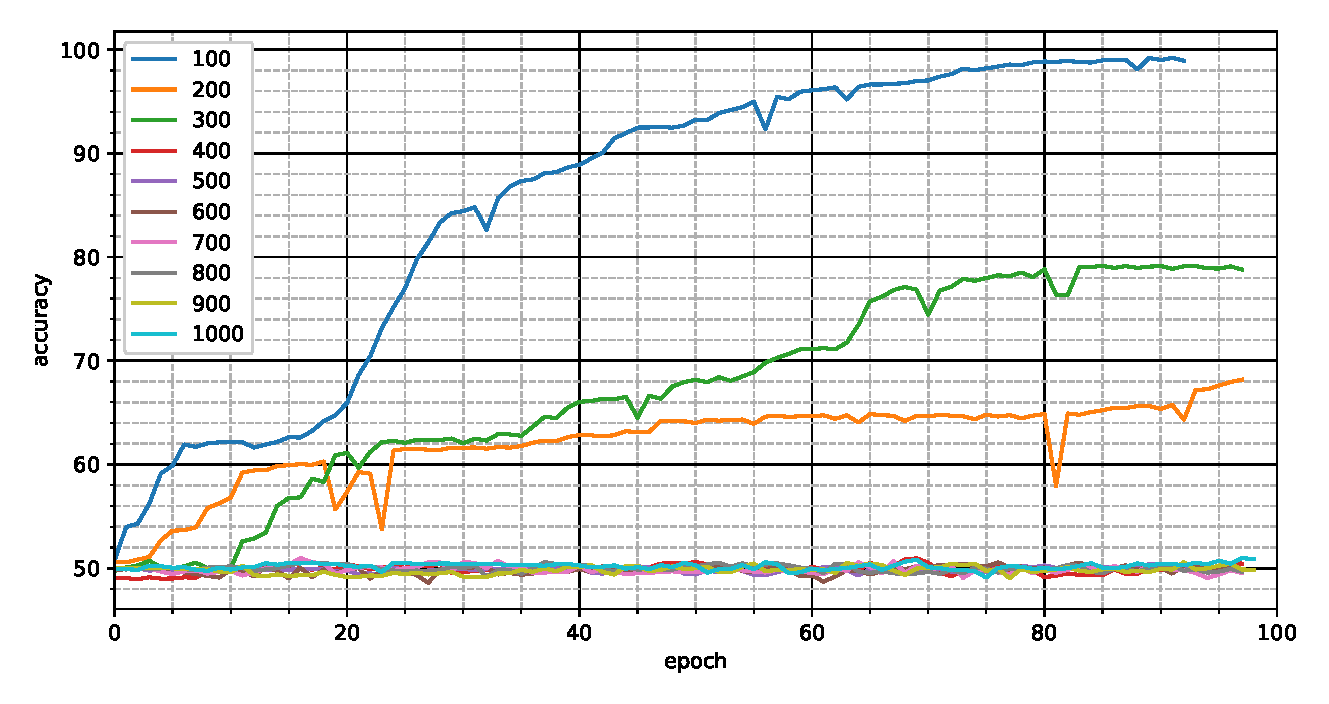
\includegraphics[width=\floatwidth]{imgMax/accuracy-base.eps}
  \caption{Accuracy of plain \ac{gru} on $\mathcal{D}^{(m)}$ for different dimensions of $m$.}
  \label{fig:testAccBase}
\end{figure}

\begin{figure}
  \centering
  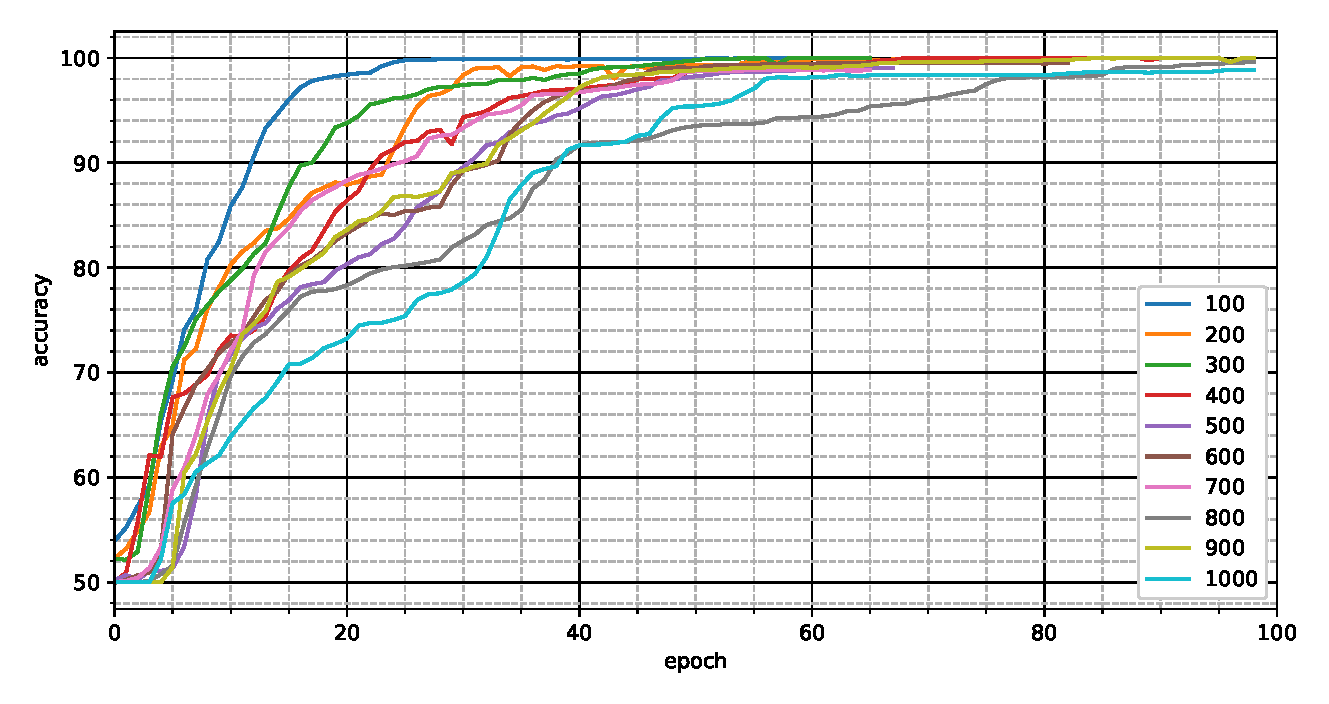
\includegraphics[width=\floatwidth]{imgMax/accuracy-max.eps}
  \caption{Accuracy of \maxi{} on $\mathcal{D}^{(m)}$ for different dimensions of $m$.}
  \label{fig:testAccMax}
\end{figure}

In \cref{fig:testAccBase} and \cref{fig:testAccMax}, we compare
the learning curves of the two model trained on the increasing
difficulty problems. We can observe 
that \maxp{} degrades less than the baseline under the assumption of
having the same dimensionality. The interpretation for this can be
that the max pooling forces locality on the sequence, thus simplifying
the task for the underlying \ac{rnn} that at time $t$ needs to keep
track only of the neighbors of $t$ in the sequence. Thus, \maxp{} can
be used on increasingly long sequences without losing potentiality.

\begin{figure}
  \centering
  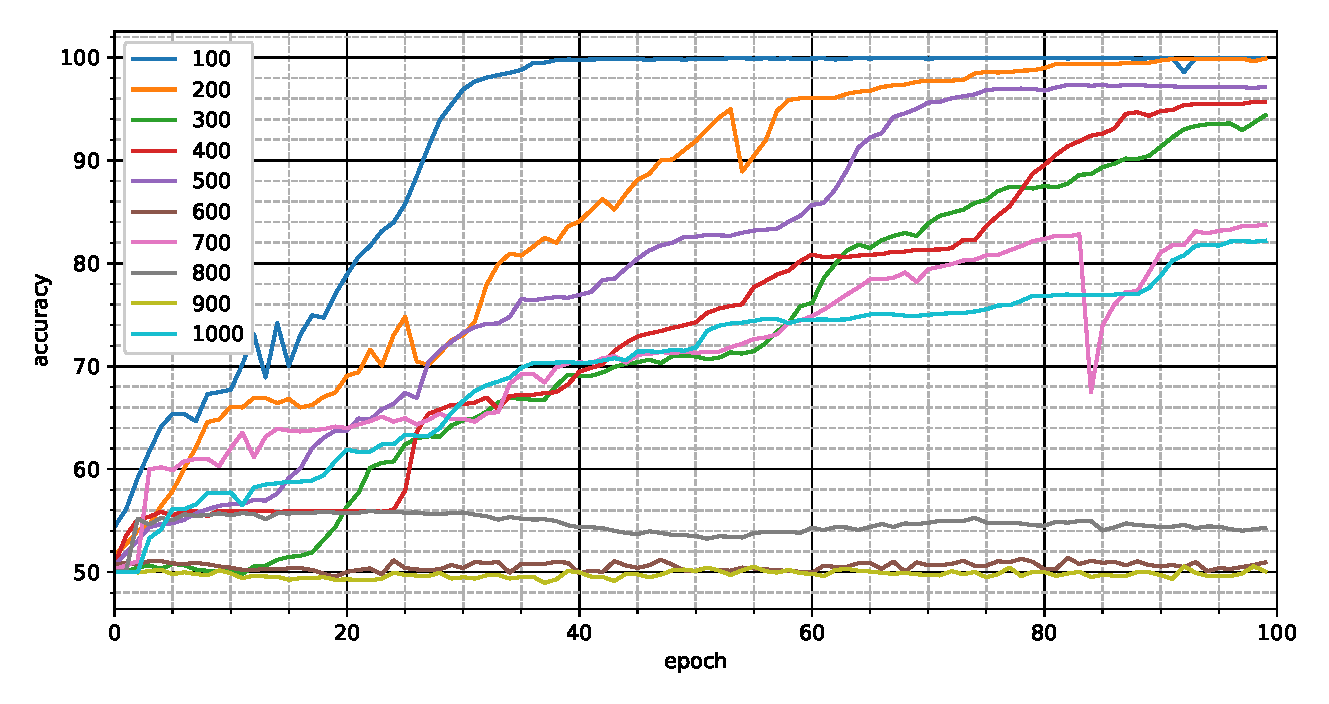
\includegraphics[width=\floatwidth]{imgMax/accuracy-int.eps}
  \caption{Accuracy of \maxi{} on $\mathcal{D}^{(m)}$ for different dimensions of $m$.}
  \label{fig:testAccInt}
\end{figure}

\begin{figure}
  \centering
  \footnotesize
  \begin{tabular}{|p{\floatwidth}|}
    \hline
    \attvisB{0}{5}{0} \attvisB{9}{6}{0} \attvisB{2}{7}{0} \attvisB{1}{7}{0} \attvisB{8}{5}{0} \attvisB{4}{5}{0} \attvisB{2}{5}{0} \attvisB{8}{5}{0} \attvisB{9}{6}{0} \attvisB{1}{6}{0} \attvisB{4}{5}{0} \attvisB{6}{5}{0} \attvisB{8}{6}{0} \attvisB{8}{5}{0} \attvisB{6}{4}{0} \attvisB{6}{5}{0} \attvisB{8}{6}{0} \attvisB{7}{7}{0} \attvisB{3}{5}{0} \attvisB{0}{5}{0} \attvisB{2}{5}{0} \attvisB{5}{5}{0} \attvisB{9}{7}{0} \attvisB{7}{7}{0} \attvisB{9}{6}{0} \attvisB{5}{5}{0} \attvisB{8}{5}{0} \attvisB{2}{5}{0} \attvisB{4}{6}{0} \attvisB{9}{6}{0} \attvisB{5}{5}{0} \attvisB{5}{5}{0} \attvisB{6}{5}{0} \attvisB{5}{6}{0} \attvisB{1}{7}{0} \attvisB{7}{7}{0} \attvisB{6}{5}{0} \attvisB{3}{5}{0} \attvisB{2}{6}{0} \attvisB{2}{5}{0} \attvisB{2}{7}{0} \attvisB{1}{6}{100} \attvisB{3}{5}{100} \attvisB{1}{100}{100} \attvisB{2}{5}{0} \attvisB{5}{5}{0} \attvisB{0}{5}{0} \attvisB{8}{5}{0} \attvisB{9}{6}{0} \attvisB{5}{5}{0} \attvisB{4}{6}{0} \attvisB{0}{5}{0} \attvisB{3}{5}{0} \attvisB{2}{5}{0} \attvisB{3}{5}{0} \attvisB{0}{5}{0} \attvisB{6}{4}{0} \attvisB{0}{5}{0} \attvisB{0}{5}{0} \attvisB{8}{5}{0} \attvisB{6}{5}{0} \attvisB{7}{7}{0} \attvisB{9}{7}{0} \attvisB{1}{6}{0} \attvisB{6}{5}{0} \attvisB{4}{6}{0} \attvisB{0}{5}{0} \attvisB{5}{5}{0} \attvisB{7}{7}{0} \attvisB{0}{5}{0} \attvisB{6}{4}{0} \attvisB{4}{6}{0} \attvisB{6}{5}{0} \attvisB{0}{6}{0} \attvisB{6}{5}{0} \attvisB{1}{6}{0} \attvisB{5}{4}{0} \attvisB{4}{6}{0} \attvisB{3}{5}{0} \attvisB{2}{6}{0} \attvisB{5}{5}{0} \attvisB{2}{5}{0} \attvisB{6}{5}{0} \attvisB{7}{7}{0} \attvisB{4}{5}{0} \attvisB{2}{5}{0} \attvisB{5}{5}{0} \attvisB{2}{5}{0} \attvisB{5}{5}{0} \attvisB{8}{5}{0} \attvisB{9}{6}{0} \attvisB{9}{6}{0} \attvisB{5}{6}{0} \attvisB{7}{7}{0} \attvisB{6}{4}{0} \attvisB{5}{5}{0} \attvisB{4}{5}{0} \attvisB{2}{6}{0} \attvisB{7}{7}{0} \attvisB{9}{6}{0}
\\
    \hline
    \attvisB{1}{7}{0} \attvisB{8}{5}{0} \attvisB{4}{6}{0} \attvisB{9}{6}{0} \attvisB{8}{6}{0} \attvisB{0}{6}{0} \attvisB{7}{7}{0} \attvisB{9}{6}{0} \attvisB{2}{5}{0} \attvisB{6}{5}{0} \attvisB{1}{6}{0} \attvisB{0}{5}{0} \attvisB{2}{5}{0} \attvisB{9}{6}{0} \attvisB{2}{5}{0} \attvisB{3}{5}{0} \attvisB{4}{6}{0} \attvisB{8}{5}{0} \attvisB{8}{5}{0} \attvisB{9}{6}{0} \attvisB{3}{5}{0} \attvisB{2}{5}{0} \attvisB{3}{5}{0} \attvisB{8}{6}{0} \attvisB{2}{5}{0} \attvisB{2}{5}{0} \attvisB{4}{6}{0} \attvisB{3}{6}{0} \attvisB{8}{6}{0} \attvisB{7}{7}{0} \attvisB{8}{5}{0} \attvisB{5}{5}{0} \attvisB{0}{5}{0} \attvisB{0}{5}{0} \attvisB{1}{6}{0} \attvisB{0}{5}{0} \attvisB{4}{5}{0} \attvisB{3}{5}{0} \attvisB{8}{6}{0} \attvisB{2}{5}{0} \attvisB{6}{4}{0} \attvisB{5}{5}{0} \attvisB{0}{5}{0} \attvisB{5}{5}{0} \attvisB{3}{5}{0} \attvisB{5}{5}{0} \attvisB{4}{5}{0} \attvisB{2}{5}{0} \attvisB{5}{5}{0} \attvisB{3}{6}{0} \attvisB{0}{5}{0} \attvisB{9}{6}{0} \attvisB{5}{6}{0} \attvisB{7}{7}{0} \attvisB{2}{5}{0} \attvisB{9}{6}{0} \attvisB{0}{6}{0} \attvisB{0}{5}{0} \attvisB{1}{7}{0} \attvisB{7}{7}{0} \attvisB{7}{7}{0} \attvisB{7}{6}{0} \attvisB{9}{6}{0} \attvisB{1}{7}{0} \attvisB{2}{6}{0} \attvisB{6}{5}{0} \attvisB{6}{4}{0} \attvisB{9}{6}{0} \attvisB{8}{6}{0} \attvisB{5}{5}{0} \attvisB{8}{6}{0} \attvisB{1}{7}{0} \attvisB{7}{7}{0} \attvisB{1}{7}{0} \attvisB{6}{4}{0} \attvisB{4}{6}{0} \attvisB{6}{5}{0} \attvisB{5}{6}{0} \attvisB{2}{6}{0} \attvisB{7}{7}{0} \attvisB{0}{6}{0} \attvisB{0}{5}{0} \attvisB{9}{6}{0} \attvisB{6}{4}{0} \attvisB{8}{7}{0} \attvisB{7}{7}{0} \attvisB{6}{5}{0} \attvisB{7}{7}{0} \attvisB{4}{5}{0} \attvisB{2}{5}{0} \attvisB{3}{5}{0} \attvisB{1}{6}{0} \attvisB{8}{5}{0} \attvisB{9}{6}{0} \attvisB{2}{5}{0} \attvisB{6}{5}{0} \attvisB{7}{7}{0} \attvisB{1}{7}{0} \attvisB{4}{6}{0} \attvisB{7}{7}{0}
\\
    \hline
    \attvisB{3}{5}{0} \attvisB{2}{6}{0} \attvisB{8}{5}{0} \attvisB{4}{5}{0} \attvisB{0}{6}{0} \attvisB{7}{6}{0} \attvisB{1}{6}{0} \attvisB{4}{5}{0} \attvisB{8}{5}{0} \attvisB{0}{5}{0} \attvisB{4}{5}{0} \attvisB{2}{5}{0} \attvisB{9}{6}{0} \attvisB{6}{4}{0} \attvisB{3}{6}{0} \attvisB{6}{6}{0} \attvisB{1}{6}{0} \attvisB{5}{4}{0} \attvisB{5}{5}{0} \attvisB{9}{7}{0} \attvisB{7}{7}{0} \attvisB{3}{5}{0} \attvisB{4}{6}{0} \attvisB{0}{5}{0} \attvisB{5}{5}{0} \attvisB{0}{4}{0} \attvisB{2}{5}{0} \attvisB{8}{5}{100} \attvisB{0}{5}{100} \attvisB{9}{6}{100} \attvisB{0}{100}{0} \attvisB{9}{6}{0} \attvisB{3}{5}{0} \attvisB{4}{5}{0} \attvisB{6}{5}{0} \attvisB{5}{5}{0} \attvisB{4}{6}{0} \attvisB{9}{7}{0} \attvisB{6}{5}{0} \attvisB{1}{6}{0} \attvisB{5}{4}{0} \attvisB{5}{5}{0} \attvisB{6}{4}{0} \attvisB{0}{5}{0} \attvisB{3}{5}{0} \attvisB{5}{5}{0} \attvisB{7}{7}{0} \attvisB{5}{4}{0} \attvisB{3}{5}{0} \attvisB{9}{5}{0} \attvisB{4}{6}{0} \attvisB{5}{5}{0} \attvisB{0}{5}{0} \attvisB{1}{7}{0} \attvisB{1}{6}{0} \attvisB{9}{6}{0} \attvisB{5}{6}{0} \attvisB{9}{6}{0} \attvisB{0}{6}{0} \attvisB{0}{6}{0} \attvisB{7}{6}{0} \attvisB{0}{5}{0} \attvisB{3}{5}{0} \attvisB{2}{5}{0} \attvisB{6}{5}{0} \attvisB{7}{7}{0} \attvisB{0}{7}{0} \attvisB{7}{6}{0} \attvisB{4}{6}{0} \attvisB{8}{5}{0} \attvisB{8}{5}{0} \attvisB{0}{5}{0} \attvisB{1}{7}{0} \attvisB{7}{7}{0} \attvisB{6}{5}{0} \attvisB{5}{5}{0} \attvisB{2}{5}{0} \attvisB{2}{5}{0} \attvisB{0}{5}{0} \attvisB{9}{6}{0} \attvisB{4}{6}{0} \attvisB{9}{6}{0} \attvisB{7}{6}{0} \attvisB{4}{6}{0} \attvisB{6}{5}{0} \attvisB{6}{5}{0} \attvisB{5}{6}{0} \attvisB{1}{6}{0} \attvisB{9}{6}{0} \attvisB{6}{4}{0} \attvisB{6}{6}{0} \attvisB{7}{7}{0} \attvisB{2}{6}{0} \attvisB{1}{6}{0} \attvisB{9}{6}{0} \attvisB{8}{7}{0} \attvisB{7}{7}{0} \attvisB{5}{4}{0} \attvisB{6}{4}{0} \attvisB{5}{5}{0}
\\
    \hline
    \attvisB{7}{7}{0} \attvisB{1}{6}{0} \attvisB{0}{5}{0} \attvisB{8}{5}{0} \attvisB{9}{6}{0} \attvisB{9}{6}{0} \attvisB{0}{6}{0} \attvisB{8}{5}{0} \attvisB{3}{5}{0} \attvisB{5}{5}{0} \attvisB{8}{6}{0} \attvisB{1}{6}{0} \attvisB{9}{6}{0} \attvisB{4}{6}{0} \attvisB{9}{6}{0} \attvisB{2}{5}{0} \attvisB{6}{4}{0} \attvisB{0}{6}{0} \attvisB{4}{5}{0} \attvisB{2}{6}{0} \attvisB{7}{7}{0} \attvisB{0}{5}{0} \attvisB{0}{6}{0} \attvisB{6}{5}{0} \attvisB{1}{6}{0} \attvisB{2}{5}{0} \attvisB{0}{6}{0} \attvisB{7}{6}{0} \attvisB{3}{5}{0} \attvisB{5}{5}{0} \attvisB{2}{6}{0} \attvisB{7}{7}{0} \attvisB{4}{5}{0} \attvisB{4}{5}{0} \attvisB{6}{5}{0} \attvisB{2}{5}{0} \attvisB{5}{5}{0} \attvisB{5}{5}{0} \attvisB{8}{5}{0} \attvisB{4}{5}{0} \attvisB{4}{5}{0} \attvisB{8}{5}{0} \attvisB{4}{6}{0} \attvisB{3}{6}{0} \attvisB{7}{7}{0} \attvisB{2}{5}{0} \attvisB{3}{6}{0} \attvisB{5}{5}{0} \attvisB{1}{7}{0} \attvisB{7}{7}{0} \attvisB{1}{7}{0} \attvisB{7}{7}{0} \attvisB{5}{5}{0} \attvisB{5}{5}{0} \attvisB{2}{5}{0} \attvisB{5}{5}{0} \attvisB{4}{7}{0} \attvisB{5}{6}{0} \attvisB{1}{6}{0} \attvisB{6}{5}{0} \attvisB{9}{6}{0} \attvisB{3}{5}{0} \attvisB{4}{6}{0} \attvisB{3}{5}{0} \attvisB{6}{5}{0} \attvisB{0}{6}{0} \attvisB{9}{6}{0} \attvisB{6}{5}{0} \attvisB{1}{7}{0} \attvisB{8}{5}{0} \attvisB{2}{5}{0} \attvisB{0}{6}{0} \attvisB{7}{7}{0} \attvisB{3}{5}{0} \attvisB{1}{6}{0} \attvisB{0}{5}{0} \attvisB{6}{5}{0} \attvisB{1}{7}{0} \attvisB{1}{6}{0} \attvisB{6}{4}{0} \attvisB{8}{5}{0} \attvisB{0}{5}{0} \attvisB{4}{6}{0} \attvisB{3}{6}{0} \attvisB{7}{7}{0} \attvisB{0}{5}{0} \attvisB{6}{4}{0} \attvisB{2}{5}{0} \attvisB{3}{5}{0} \attvisB{2}{6}{0} \attvisB{0}{5}{0} \attvisB{9}{6}{0} \attvisB{0}{6}{0} \attvisB{8}{5}{0} \attvisB{5}{4}{0} \attvisB{5}{5}{0} \attvisB{9}{6}{0} \attvisB{6}{5}{0} \attvisB{9}{6}{0} \attvisB{9}{6}{0}
\\
    \hline
    \attvisB{0}{5}{0} \attvisB{3}{5}{0} \attvisB{3}{5}{100} \attvisB{9}{6}{100} \attvisB{7}{100}{100} \attvisB{3}{5}{0} \attvisB{6}{5}{0} \attvisB{8}{6}{0} \attvisB{6}{5}{0} \attvisB{2}{7}{0} \attvisB{1}{6}{0} \attvisB{5}{5}{0} \attvisB{2}{5}{0} \attvisB{4}{5}{0} \attvisB{3}{5}{0} \attvisB{8}{6}{0} \attvisB{4}{7}{0} \attvisB{7}{6}{0} \attvisB{2}{6}{0} \attvisB{1}{7}{0} \attvisB{7}{7}{0} \attvisB{2}{5}{0} \attvisB{9}{6}{0} \attvisB{2}{5}{0} \attvisB{3}{5}{0} \attvisB{1}{6}{0} \attvisB{6}{5}{0} \attvisB{0}{6}{0} \attvisB{0}{6}{0} \attvisB{7}{6}{0} \attvisB{2}{6}{0} \attvisB{0}{5}{0} \attvisB{1}{6}{0} \attvisB{4}{5}{0} \attvisB{3}{5}{0} \attvisB{2}{6}{0} \attvisB{0}{5}{0} \attvisB{9}{6}{0} \attvisB{4}{6}{0} \attvisB{3}{5}{0} \attvisB{6}{4}{0} \attvisB{8}{5}{0} \attvisB{8}{5}{0} \attvisB{0}{6}{0} \attvisB{6}{5}{0} \attvisB{1}{6}{0} \attvisB{2}{5}{0} \attvisB{2}{5}{0} \attvisB{6}{5}{0} \attvisB{7}{7}{0} \attvisB{2}{5}{0} \attvisB{6}{4}{0} \attvisB{5}{5}{0} \attvisB{6}{4}{0} \attvisB{6}{5}{0} \attvisB{4}{6}{0} \attvisB{5}{5}{0} \attvisB{5}{5}{0} \attvisB{2}{5}{0} \attvisB{2}{5}{0} \attvisB{2}{6}{0} \attvisB{1}{6}{0} \attvisB{2}{5}{0} \attvisB{3}{6}{0} \attvisB{7}{7}{0} \attvisB{1}{7}{0} \attvisB{8}{5}{0} \attvisB{8}{5}{0} \attvisB{8}{5}{0} \attvisB{2}{5}{0} \attvisB{8}{5}{0} \attvisB{5}{4}{0} \attvisB{8}{5}{0} \attvisB{3}{5}{0} \attvisB{4}{6}{0} \attvisB{8}{5}{0} \attvisB{5}{5}{0} \attvisB{6}{4}{0} \attvisB{8}{6}{0} \attvisB{0}{5}{0} \attvisB{3}{5}{0} \attvisB{6}{4}{0} \attvisB{9}{6}{0} \attvisB{0}{6}{0} \attvisB{6}{4}{0} \attvisB{0}{5}{0} \attvisB{4}{5}{0} \attvisB{0}{5}{0} \attvisB{8}{5}{0} \attvisB{2}{5}{0} \attvisB{4}{6}{0} \attvisB{5}{5}{0} \attvisB{5}{5}{0} \attvisB{2}{5}{0} \attvisB{4}{5}{0} \attvisB{0}{5}{0} \attvisB{8}{5}{0} \attvisB{3}{5}{0} \attvisB{0}{5}{0} \attvisB{8}{5}{0}
\\
    \hline
    \attvisB{1}{7}{0} \attvisB{5}{5}{0} \attvisB{5}{5}{0} \attvisB{8}{5}{0} \attvisB{8}{5}{0} \attvisB{9}{6}{0} \attvisB{8}{6}{0} \attvisB{8}{5}{0} \attvisB{0}{5}{0} \attvisB{3}{5}{0} \attvisB{5}{5}{0} \attvisB{2}{5}{0} \attvisB{0}{5}{0} \attvisB{0}{5}{0} \attvisB{2}{6}{0} \attvisB{7}{7}{0} \attvisB{5}{4}{0} \attvisB{4}{6}{0} \attvisB{2}{5}{0} \attvisB{4}{7}{0} \attvisB{7}{7}{0} \attvisB{0}{5}{0} \attvisB{4}{5}{0} \attvisB{6}{5}{0} \attvisB{5}{5}{0} \attvisB{0}{5}{0} \attvisB{4}{5}{0} \attvisB{0}{5}{0} \attvisB{2}{5}{0} \attvisB{6}{5}{0} \attvisB{7}{7}{0} \attvisB{9}{6}{0} \attvisB{6}{5}{0} \attvisB{9}{6}{0} \attvisB{2}{5}{0} \attvisB{4}{6}{0} \attvisB{7}{7}{0} \attvisB{5}{4}{0} \attvisB{8}{5}{0} \attvisB{4}{7}{0} \attvisB{1}{6}{0} \attvisB{6}{4}{0} \attvisB{5}{6}{0} \attvisB{5}{5}{0} \attvisB{1}{7}{0} \attvisB{1}{6}{0} \attvisB{9}{6}{0} \attvisB{8}{6}{0} \attvisB{2}{5}{0} \attvisB{6}{4}{0} \attvisB{2}{5}{0} \attvisB{6}{4}{0} \attvisB{8}{6}{0} \attvisB{5}{5}{0} \attvisB{4}{6}{0} \attvisB{0}{5}{0} \attvisB{5}{4}{0} \attvisB{5}{5}{0} \attvisB{9}{6}{0} \attvisB{2}{6}{0} \attvisB{5}{5}{0} \attvisB{6}{4}{0} \attvisB{2}{5}{0} \attvisB{9}{6}{0} \attvisB{0}{6}{0} \attvisB{3}{5}{0} \attvisB{8}{6}{0} \attvisB{4}{5}{0} \attvisB{3}{6}{0} \attvisB{7}{7}{0} \attvisB{8}{5}{0} \attvisB{9}{6}{0} \attvisB{1}{7}{0} \attvisB{8}{5}{0} \attvisB{3}{6}{0} \attvisB{7}{7}{0} \attvisB{8}{5}{0} \attvisB{9}{6}{0} \attvisB{8}{6}{0} \attvisB{1}{6}{0} \attvisB{9}{6}{0} \attvisB{6}{4}{0} \attvisB{6}{4}{0} \attvisB{6}{5}{0} \attvisB{7}{7}{0} \attvisB{4}{6}{0} \attvisB{9}{6}{0} \attvisB{4}{6}{0} \attvisB{4}{7}{0} \attvisB{7}{7}{0} \attvisB{8}{5}{0} \attvisB{0}{5}{0} \attvisB{1}{6}{0} \attvisB{8}{5}{0} \attvisB{3}{6}{0} \attvisB{7}{7}{0} \attvisB{8}{5}{0} \attvisB{4}{5}{0} \attvisB{6}{5}{0} \attvisB{6}{5}{0}
\\
    \hline
  \end{tabular}
  \caption{Visualization of outputs prior to the max pooling of
    \maxi{} for some 
    samples. Red boxes represent the prime numbers ground
    truth, green highlighting represents the values of $u_t$ in
    \eqref{eq:maxModelF}.}
  \label{fig:testAttention}
\end{figure}

Regarding the interpretable models, we can observe that
the degradation of the interpretable \maxi{} model in
fig. \ref{fig:testAccInt} is worse 
compared to \maxp{} in fig. \ref{fig:testAccMax},
but is still better compared to the base \ac{gru} model in
fig. \ref{fig:testAccBase}. Conversely, the interpretable model can be
used to gain
some insights on the decision process. As visible in
fig. \ref{fig:testAttention}, the model performs the classification
task focusing on 
the part of the sequences where the prime numbers are present. The
reasons why \maxi{} is not scaling as \maxp{} can be found in the fact
that in the interpretable setting we basically moved the aggregation
from before to after the classification part. The max pooling in
\maxi{} does not have the same localizing effect on the underlying
part. Nevertheless, it still has some effect on simplifying the
task.

\begin{figure}
  \centering
  \footnotesize
  \begin{tabular}{|p{\floatwidth}|}
    \hline
    \attvisB{3}{0}{0} \attvisB{6}{0}{0} \attvisB{2}{0}{0} \attvisB{9}{0}{0} \attvisB{4}{0}{0} \attvisB{8}{0}{0} \attvisB{0}{0}{0} \attvisB{6}{0}{0} \attvisB{3}{0}{0} \attvisB{0}{0}{0} \attvisB{4}{0}{0} \attvisB{7}{0}{0} \attvisB{6}{0}{0} \attvisB{5}{0}{0} \attvisB{6}{0}{0} \attvisB{7}{0}{0} \attvisB{5}{0}{0} \attvisB{9}{0}{0} \attvisB{8}{0}{0} \attvisB{6}{0}{0} \attvisB{5}{0}{0} \attvisB{1}{0}{0} \attvisB{2}{0}{0} \attvisB{6}{0}{0} \attvisB{7}{0}{0} \attvisB{8}{0}{0} \attvisB{8}{0}{0} \attvisB{2}{0}{0} \attvisB{2}{0}{0} \attvisB{5}{0}{0} \attvisB{3}{0}{0} \attvisB{1}{0}{0} \attvisB{6}{0}{0} \attvisB{4}{0}{0} \attvisB{4}{0}{0} \attvisB{0}{0}{0} \attvisB{7}{0}{0} \attvisB{4}{0}{0} \attvisB{8}{0}{100} \attvisB{6}{78}{100} \attvisB{3}{0}{100} \attvisB{2}{0}{0} \attvisB{0}{20}{0} \attvisB{6}{0}{0} \attvisB{0}{0}{0} \attvisB{6}{0}{0} \attvisB{2}{0}{0} \attvisB{1}{0}{0} \attvisB{5}{0}{0} \attvisB{5}{0}{0} \attvisB{8}{0}{0} \attvisB{2}{0}{0} \attvisB{4}{0}{0} \attvisB{8}{0}{0} \attvisB{9}{0}{0} \attvisB{0}{0}{0} \attvisB{1}{0}{0} \attvisB{1}{0}{0} \attvisB{2}{0}{0} \attvisB{3}{0}{0} \attvisB{2}{0}{0} \attvisB{7}{0}{0} \attvisB{5}{0}{0} \attvisB{0}{0}{0} \attvisB{1}{0}{0} \attvisB{8}{0}{0} \attvisB{5}{0}{0} \attvisB{2}{0}{0} \attvisB{4}{0}{0} \attvisB{4}{0}{0} \attvisB{7}{0}{0} \attvisB{5}{0}{0} \attvisB{3}{0}{0} \attvisB{6}{0}{0} \attvisB{4}{0}{0} \attvisB{9}{0}{0} \attvisB{0}{0}{0} \attvisB{6}{0}{0} \attvisB{6}{0}{0} \attvisB{2}{0}{0} \attvisB{5}{0}{0} \attvisB{5}{0}{0} \attvisB{5}{0}{0} \attvisB{1}{0}{0} \attvisB{6}{0}{0} \attvisB{1}{0}{0} \attvisB{0}{0}{0} \attvisB{0}{0}{0} \attvisB{6}{0}{0} \attvisB{7}{0}{0} \attvisB{5}{0}{0} \attvisB{9}{0}{0} \attvisB{7}{0}{0} \attvisB{4}{0}{0} \attvisB{4}{0}{0} \attvisB{5}{0}{0} \attvisB{2}{0}{0} \attvisB{4}{0}{0} \attvisB{9}{0}{0} \attvisB{2}{0}{0}

\\
    \hline
    \attvisB{5}{0}{0} \attvisB{3}{0}{0} \attvisB{6}{0}{0} \attvisB{9}{0}{0} \attvisB{0}{0}{0} \attvisB{9}{0}{0} \attvisB{1}{0}{0} \attvisB{8}{0}{0} \attvisB{0}{0}{0} \attvisB{1}{0}{0} \attvisB{5}{0}{0} \attvisB{4}{0}{0} \attvisB{5}{0}{0} \attvisB{0}{0}{0} \attvisB{4}{0}{0} \attvisB{7}{0}{0} \attvisB{1}{0}{0} \attvisB{6}{0}{0} \attvisB{2}{0}{0} \attvisB{3}{0}{0} \attvisB{2}{0}{0} \attvisB{9}{0}{0} \attvisB{2}{0}{0} \attvisB{6}{0}{0} \attvisB{8}{0}{0} \attvisB{8}{0}{0} \attvisB{2}{0}{0} \attvisB{6}{0}{0} \attvisB{1}{0}{0} \attvisB{1}{0}{0} \attvisB{2}{0}{0} \attvisB{3}{0}{0} \attvisB{6}{0}{0} \attvisB{3}{0}{0} \attvisB{6}{0}{0} \attvisB{4}{0}{0} \attvisB{4}{0}{0} \attvisB{6}{0}{0} \attvisB{6}{0}{0} \attvisB{8}{0}{0} \attvisB{9}{0}{0} \attvisB{9}{0}{0} \attvisB{3}{0}{0} \attvisB{5}{0}{0} \attvisB{6}{0}{0} \attvisB{4}{0}{0} \attvisB{2}{0}{0} \attvisB{4}{0}{0} \attvisB{7}{0}{0} \attvisB{0}{0}{0} \attvisB{3}{0}{0} \attvisB{3}{0}{0} \attvisB{8}{0}{0} \attvisB{5}{0}{0} \attvisB{5}{0}{0} \attvisB{4}{0}{0} \attvisB{6}{0}{0} \attvisB{9}{0}{0} \attvisB{2}{0}{0} \attvisB{3}{0}{0} \attvisB{2}{0}{0} \attvisB{9}{0}{0} \attvisB{5}{0}{0} \attvisB{5}{0}{0} \attvisB{3}{0}{0} \attvisB{5}{0}{0} \attvisB{7}{0}{0} \attvisB{8}{0}{0} \attvisB{0}{0}{0} \attvisB{4}{0}{0} \attvisB{7}{0}{0} \attvisB{1}{0}{0} \attvisB{3}{0}{0} \attvisB{6}{0}{0} \attvisB{6}{0}{0} \attvisB{3}{0}{0} \attvisB{8}{0}{0} \attvisB{8}{0}{0} \attvisB{8}{0}{0} \attvisB{8}{0}{0} \attvisB{6}{0}{0} \attvisB{9}{0}{0} \attvisB{6}{0}{0} \attvisB{0}{0}{0} \attvisB{6}{0}{0} \attvisB{4}{0}{100} \attvisB{0}{0}{100} \attvisB{1}{0}{100} \attvisB{5}{8}{0} \attvisB{4}{8}{0} \attvisB{9}{8}{0} \attvisB{5}{8}{0} \attvisB{5}{8}{0} \attvisB{5}{8}{0} \attvisB{9}{8}{0} \attvisB{7}{8}{0} \attvisB{6}{8}{0} \attvisB{5}{8}{0} \attvisB{8}{8}{0} \attvisB{4}{8}{0}

\\
    \hline
    \attvisB{3}{0}{0} \attvisB{2}{0}{0} \attvisB{8}{0}{0} \attvisB{4}{0}{0} \attvisB{0}{0}{0} \attvisB{7}{0}{0} \attvisB{1}{0}{0} \attvisB{4}{0}{0} \attvisB{8}{0}{0} \attvisB{0}{0}{0} \attvisB{4}{0}{0} \attvisB{2}{0}{0} \attvisB{9}{0}{0} \attvisB{6}{0}{0} \attvisB{3}{0}{0} \attvisB{6}{0}{0} \attvisB{1}{0}{0} \attvisB{5}{0}{0} \attvisB{5}{0}{0} \attvisB{9}{0}{0} \attvisB{7}{0}{0} \attvisB{3}{0}{0} \attvisB{4}{0}{0} \attvisB{0}{0}{0} \attvisB{5}{0}{0} \attvisB{0}{0}{0} \attvisB{2}{0}{0} \attvisB{8}{0}{100} \attvisB{0}{0}{100} \attvisB{9}{0}{100} \attvisB{0}{1}{0} \attvisB{9}{1}{0} \attvisB{3}{1}{0} \attvisB{4}{1}{0} \attvisB{6}{1}{0} \attvisB{5}{1}{0} \attvisB{4}{1}{0} \attvisB{9}{1}{0} \attvisB{6}{1}{0} \attvisB{1}{1}{0} \attvisB{5}{1}{0} \attvisB{5}{1}{0} \attvisB{6}{1}{0} \attvisB{0}{1}{0} \attvisB{3}{1}{0} \attvisB{5}{1}{0} \attvisB{7}{1}{0} \attvisB{5}{1}{0} \attvisB{3}{1}{0} \attvisB{9}{1}{0} \attvisB{4}{1}{0} \attvisB{5}{1}{0} \attvisB{0}{1}{0} \attvisB{1}{1}{0} \attvisB{1}{1}{0} \attvisB{9}{1}{0} \attvisB{5}{1}{0} \attvisB{9}{1}{0} \attvisB{0}{1}{0} \attvisB{0}{1}{0} \attvisB{7}{1}{0} \attvisB{0}{1}{0} \attvisB{3}{1}{0} \attvisB{2}{1}{0} \attvisB{6}{1}{0} \attvisB{7}{1}{0} \attvisB{0}{1}{0} \attvisB{7}{1}{0} \attvisB{4}{1}{0} \attvisB{8}{1}{0} \attvisB{8}{1}{0} \attvisB{0}{1}{0} \attvisB{1}{1}{0} \attvisB{7}{1}{0} \attvisB{6}{1}{0} \attvisB{5}{1}{0} \attvisB{2}{1}{0} \attvisB{2}{1}{0} \attvisB{0}{1}{0} \attvisB{9}{1}{0} \attvisB{4}{1}{0} \attvisB{9}{1}{0} \attvisB{7}{1}{0} \attvisB{4}{1}{0} \attvisB{6}{1}{0} \attvisB{6}{1}{0} \attvisB{5}{1}{0} \attvisB{1}{1}{0} \attvisB{9}{1}{0} \attvisB{6}{1}{0} \attvisB{6}{1}{0} \attvisB{7}{1}{0} \attvisB{2}{1}{0} \attvisB{1}{1}{0} \attvisB{9}{1}{0} \attvisB{8}{1}{0} \attvisB{7}{1}{0} \attvisB{5}{1}{0} \attvisB{6}{1}{0} \attvisB{5}{1}{0}

\\
    \hline
  \end{tabular}
  \caption{Visualization of weighted features after softmax in
    \softmaxi{} for some
    positive samples. Red boxes represent the prime numbers ground
    truth, green highlighting represents the values of
    $a_t(\vect{u};\theta^a)u_t$ in
    \eqref{eq:aggregation}.}
  \label{fig:testAttentionSoft}
\end{figure}
We wanted also to compare the difference of the max vs attention
aggregation. In 
\cref{fig:testAttentionSoft} we have empirical evidence that the
attention aggregation is not sufficient to guarantee the model
interpretability (at least in this setting). This can be explained
with the fact that the softmax function does 
not avoid the learning of underlying
distribute representations. 
On the loss calculation, the effects of a
distribution with high variance before the aggregation are the 
same to the ones of a distribution with lower variance. Thus, the \ac{sgd} does
not favor focused representations in $u_t$.

\begin{figure}
  \centering
  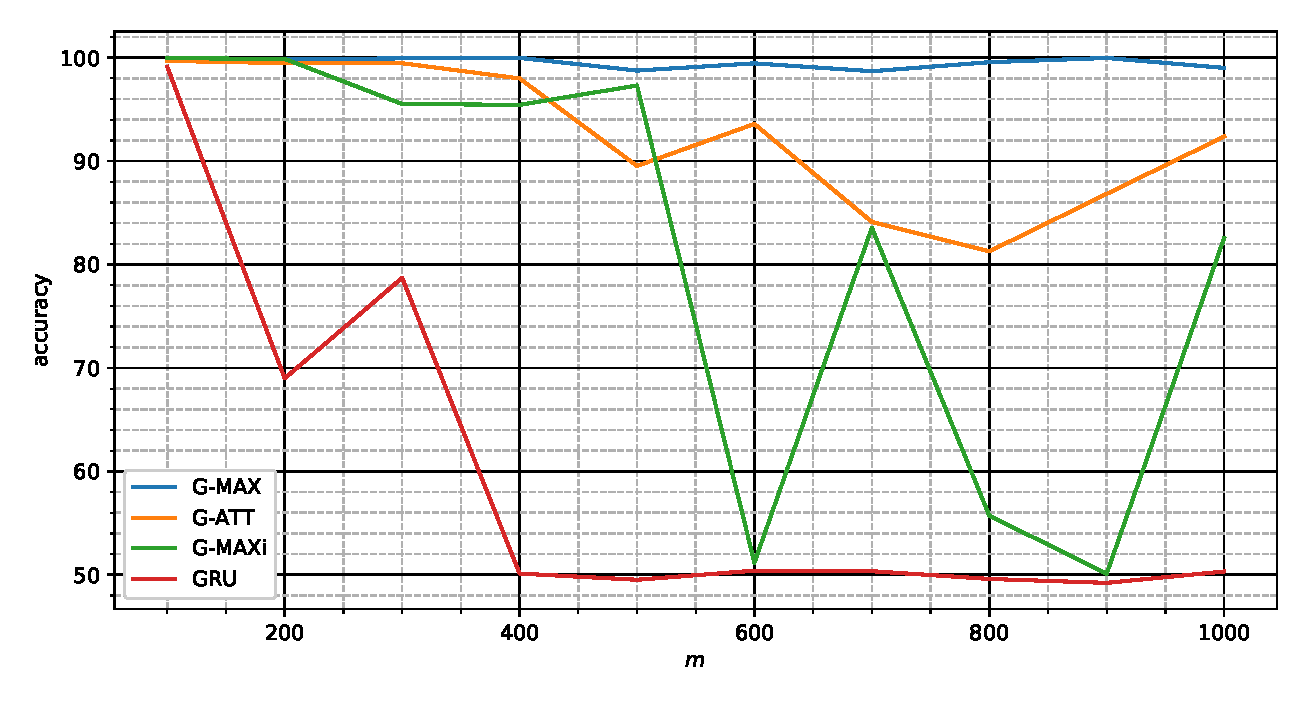
\includegraphics[width=\floatwidth]{imgMax/maxBaseDiff.eps}
  \caption{Max reached accuracy of \maxp{}, \softmax{}, \maxi{}, and
    base \ac{gru} models on
    $\mathcal{D}^{(m)}$ for different dimensions of $m$.} 
  \label{fig:testAccDiff}
\end{figure}
In \cref{fig:testAccDiff}, we show the maximum reached accuracy for the
models, summarizing
\cref{fig:testAccBase,fig:testAccMax,fig:testAccInt} and also adding
\softmax{}. From this plot we can evince that \softmax{} degrades
faster than \maxp{}. This can be due to the fact that the attention,
using a softmax on all the underlying representations,
still needs to rely on the entire sequence. Thus, there is not the
strong focusing effect of the max aggregation.


\section{Aggregation, interpretability, hierarchical}
\label{ch:icdo}
In these experiments we further refined the dataset. We removed duplicate
reports and reports labeled with extremely rare (1048
samples that do not
appear in all three of training, validation, and test sets) ICD-O3
codes. In the end we
obtained 
a dataset suitable for supervised learning consisting of $85\,170$
labeled records, over $203$ morphological classes, and $68$
topological classes.

We defined two multi-class classification tasks: (1) main tumor site
prediction ($68$ mutually exclusive classes) and (2) morphology
prediction ($203$ mutually exclusive
classes). Although the two tasks maybe somewhat correlated, we did not
attempt multi-task approaches given the small number of tasks and
large enough size of the dataset.

We decided to arrange our experiments on cancer
data in 
a setting that simulates a predictive task. We sorted the medical
records by insertion date, then we used the most recent $80\%$ of
records as test 
dataset, an equal amount of the remaining most recent records as
validation dataset, and the rest as training dataset. The splitting of
data resulted in $51\,101$ records for training,
$17\,034$ for validation, and $17\,035$ for test datasets.

We used the text in the $1.5$ millions unlabeled records, plus the
text in training datasets to train \ac{glove} word
vectors representations.

We trained the models \maxp{}, \softmax{}, \maxi{}, \maxh{}, and
\softmaxh{} on both prediction tasks. We found the hyperparameters 
configurations doing grid search on the space explained in
\cref{sec:hyperparameters}. 
% \maxi{} have one \ac{gru} layer of dimension $256$
% for \eqref{eq:maxModelRL} and \eqref{eq:maxModelRR}, 1 layer of
% output dimension $68$ with aggregating function \eqref{eq:aggregation}
% for \eqref{eq:maxModelF}, and zero layers for \eqref{eq:maxModelC}. 
% \maxp{} have
% one \ac{gru} layer with
% dimension $128$ for \eqref{eq:maxModelRL} and \eqref{eq:maxModelRR},
% one \ac{mlp} layer of dimension $512$ with aggregating function
% \eqref{eq:aggregation} for \eqref{eq:maxModelF}, and
% one layer of output dimension $68$ for \eqref{eq:maxModelC}.

We trained the models minimizing categorical cross entropy with Adam
\cite{kingma2014adam} using a starting learning rate of $0.001$. The
experiments were performed in \emph{PyTorch} on machines with
\emph{GeForce RTX 2080 Ti} 
GPU using batches of $32$ samples.

% We compared \maxp{} and \maxi{} with the baseline \gru{}  and with
% \bert{} pretrained on the 
% same data where \ac{glove} where trained for the other models, and
% fine-tuned on the training set.


\subsection{Hyperparameters}\label{sec:hyperparameters}
The hyperparameters of \eqref{eq:embed}~-~\eqref{eq:maxModelC}
and \eqref{eq:embedH}~-~\eqref{eq:maxModelCH} control the structure of
the model.

$\xi^e$ is associated with the embedding layer $E$ and in our case
refers to \ac{glove} 
hyperparameters~\cite{pennington_glove:_2014}. With an intrinsic
evaluation, we found that the better configuration was $60$ for the vector
size, $15$ for the window size, and $50$ iterations. $\xi^f$,
$\xi^r$, $\xi'^{f}$, and $\xi'^{r}$ define the number of
\ac{gru} layers ($\xi_{(l)}$) and the number of unit per each layer
($\xi_{(d)}$) respectively for $F$, $R$, $F'$, and $R'$. 
$G$ is a \ac{mlp}, $\xi^h$ controls the number of
layers and their dimension. Regarding $F$, $R$, and $G$, we decided to
have all the stacked layer with 
the same dimension to limit the
hyperparameters space. $\xi^a$ and $\xi'^a$ control the
kind of aggregating function of $A$ and $A'$ respectively and, in case
of \emph{attention}, 
it controls the dimension of the attention layer. Finally, $\xi^c$ controls the
data-dependent output dimension of $g$.

In \maxp{} we used the \emph{max} aggregation
function 
in the plain model of \cref{sec:modelh}. We determined the
hyperparameters evaluating the validation set in the space (with the
better configuration underlined):
\begin{align*}
  \xi_{(l)}^f=\xi_{(l)}^r&\in[\underline{1},2],\\
  \xi_{(d)}^f=\xi_{(d)}^r&\in[2,4,8,16,32,64,\underline{128},256,512],\\
  \xi_{(l)}^h&\in[\underline{1},2,4],\\
  \xi_{(d)}^h&\in[2,4,8,16,32,64,128,256,\underline{512},1024,2048],
\end{align*}
for the \emph{main site} task, and:
\begin{align*}
  \xi_{(l)}^f=\xi_{(l)}^r&\in[\underline{1}],\\
  \xi_{(d)}^f=\xi_{(d)}^r&\in[2,4,8,16,32,64,\underline{128},256,512],\\
  \xi_{(l)}^h&\in[\underline{1},2,4],\\
  \xi_{(d)}^h&\in[2,4,8,16,32,64,\underline{128},256,512,1024,2048],
\end{align*}
for the \emph{morphology} task.

In \softmax{} we used the \emph{attention} aggregation function in the
plain model. The hyperparameters
space was:
\begin{align*}
  \xi_{(l)}^f=\xi_{(l)}^r&\in[\underline{1}],\\
  \xi_{(d)}^f=\xi_{(d)}^r&\in[64,\underline{128},256],\\
  \xi_{(l)}^h&\in[0,\underline{1}],\\
  \xi_{(d)}^h&\in[256,\underline{512},1024],\\
  \xi_{(d)}^a&\in[128,\underline{256},512,1024],
\end{align*}
for the site, and:
\begin{align*}
  \xi_{(l)}^f=\xi_{(l)}^r&\in[\underline{1}],\\
  \xi_{(d)}^f=\xi_{(d)}^r&\in[64,128,\underline{256}],\\
  \xi_{(l)}^h&\in[0,\underline{1}],\\
  \xi_{(d)}^h&\in[64,\underline{128},256],\\
  \xi_{(d)}^a&\in[128,\underline{256},512,1024],
\end{align*}
for the morphology.

In \maxh{} we used the \emph{max} aggregation in the hierarchical
model of \cref{sec:modelh}. The hyperparameters space was:
\begin{align*}
  \xi_{(l)}^f=\xi_{(l)}^r=\xi'^f_{(l)}=\xi'^r_{(l)}&\in[\underline{1}],\\
  \xi_{(d)}^f=\xi_{(d)}^r=\xi'^f_{(d)}=\xi'^r_{(d)}&\in[32,\underline{64},128,256],\\
  \xi_{(l)}^h&\in[0,1,\underline{2},4],\\
  \xi_{(d)}^h&\in[256,512,\underline{1024},2048],\\
\end{align*}
for the site, and:
\begin{align*}
  \xi_{(l)}^f=\xi_{(l)}^r=\xi'^f_{(l)}=\xi'^r_{(l)}&\in[\underline{1}],\\
  \xi_{(d)}^f=\xi_{(d)}^r=\xi'^f_{(d)}=\xi'^r_{(d)}&\in[32,\underline{64},128,256],\\
  \xi_{(l)}^h&\in[0,\underline{1},2,4],\\
  \xi_{(d)}^h&\in[256,512,\underline{1024},2048],\\
\end{align*}
for the morphology.

In \softmaxh{} we used the \emph{attention} aggregation in the
hierarchical model. The hyperparameters space was:
\begin{align*}
  \xi_{(l)}^f=\xi_{(l)}^r=\xi'^f_{(l)}=\xi'^r_{(l)}&\in[\underline{1}],\\
  \xi_{(d)}^f=\xi_{(d)}^r=\xi'^f_{(d)}=\xi'^r_{(d)}&\in[32,64,\underline{128},256],\\
  \xi_{(l)}^h&\in[0,\underline{1},2,4],\\
  \xi_{(d)}^h&\in[256,512,\underline{1024},2048],\\
  \xi_{(d)}^a=\xi'^a_{(d)}&\in[64,\underline{128},256,512],
\end{align*}
for the site, and:
\begin{align*}
  \xi_{(l)}^f=\xi_{(l)}^r=\xi'^f_{(l)}=\xi'^r_{(l)}&\in[\underline{1}],\\
  \xi_{(d)}^f=\xi_{(d)}^r=\xi'^f_{(d)}=\xi'^r_{(d)}&\in[32,\underline{64},128,256],\\
  \xi_{(l)}^h&\in[0,\underline{1},2,4],\\
  \xi_{(d)}^h&\in[256,512,\underline{1024},2048],\\
  \xi_{(d)}^a=\xi'^a_{(d)}&\in[64,\underline{128},256,512],
\end{align*}
for the morphology.

In \maxi{} we used the \emph{max} aggregation in the plain
model. Also we set the model to be interpretable. The hyperparameters
space was: 
\begin{align*}
  \xi_{(l)}^f=\xi_{(l)}^r&\in[1,\underline{2},4],\\
  \xi_{(d)}^f=\xi_{(d)}^r&\in[2,4,8,16,32,64,\underline{128},256,512],\\
  \xi_{(l)}^h&\in[\underline{1},2,4],\\
  \xi_{(d)}^h&\in[2,4,8,16,32,64,128,256,512,1024,2048],
\end{align*}
for the site, and:
\begin{align*}
  \xi_{(l)}^f=\xi_{(l)}^r&\in[1,\underline{2},4],\\
  \xi_{(d)}^f=\xi_{(d)}^r&\in[64,128,\underline{256},512],\\
  \xi_{(l)}^h&\in[\underline{1}],\\
  \xi_{(d)}^h&\in[],
\end{align*}
for the morphology. Note that, in this setting, the dimension of the
last layer of $G$ must be equal to the output dimension of the model
(and the softmax is applied directly after the aggregation $A$,
without any layer). Thus, $\xi_{(d)}^h$ refers only to the
layers before the last one, if they exist.

Regarding \gru{}, we searched in a space of $[1,2,4]$ number of layers of
dimension in $[128,256,512,1024]$. We found that the best
configuration was using $2$ layers of dimension $256$.



% The hyperparameters $\xi=\xi^l\cup\xi^r\cup\xi^h\cup\xi^c$ define the
% structure of the model. Regarding $\xi^l=\xi^r$ they define the type
% of \ac{rnn} that in our experiments can be \ac{lstm} or \ac{gru}, the
% number of stacked \ac{rnn} layers and the dimension of each
% layer. $\xi^h$ defines the number of layers in the first
% \ac{mlp} and their
% dimensions, moreover it defines the type of aggregating function $f$
% that in our experiments can be one of
% \begin{align}
%   f(\vect{a},\vect{b}) &= \left[\max(a_1,b_1),\dots,\max(a_l,b_l)\right];\\
%   f(\vect{a},\vect{b}) &= \left[\frac{a_1+b_1}{2},\dots,\frac{a_l+b_l}{2}\right];\\
%   f(\vect{a},\vect{b}) &= \left[a_1,\dots,a_l,b_1,\dots,b_l\right].\label{eq:aggregation}
% \end{align}
% $\xi^c$ defines the number of layers and their dimensions of the
% final classifier. The number of layers defined in $\xi^h$ can be
% equal to $0$. In such case, $\vect{h}_{i,j}$ is calculated:
% \begin{equation*}
%   \vect{h}_{i,j} = f(\vect{h}^l_{i,j},\vect{h}^r_{i,j}).
% \end{equation*}
% Also the number of layers defined in $\xi^c$ can be equal to $0$. In
% such case $\vect{\hat{y}}_i$ is calculated:
% \begin{equation*}
%   \vect{\hat y}_i = \max_j(\vect{h}_{i,j}).
% \end{equation*}


\subsection{Results}

\begin{table}
  \centering
  \caption{Results on cancer data}
  \label{tab:results}
  \begin{tabular}{|c|c|c|c|c|c|}
    \hline
    &Acc.&Acc. T3&Acc. T5&MAP&K\\
    \hline
    \hline
    \textbf{Site}&&&&&\\
    \gru{}&0.8977&0.9636&0.9764&0.9331&0.8848\\
    \bert{}&0.8980&0.9623&0.9768&0.9330&0.8852\\
    \maxi{}&0.8792&0.9533&0.9610&0.9190&0.8637\\
    \maxh{}&0.8980&0.9611&0.9773&0.9329&0.8851\\
    \softmaxh{}&0.8983&0.9617&0.9760&0.9329&0.8855\\
    \softmax{}&0.9008&0.9607&0.9749&0.9341&0.8883\\
    \maxp{}&\textbf{0.9024}&\textbf{0.9658}&\textbf{0.9797}&\textbf{0.9369}&\textbf{0.8901}\\
    \hline
    \hline
    \textbf{Morpho.}&&&&&\\
    \gru{}&0.8266&0.9402&0.9602&0.8881&0.8064\\
    \bert{}&0.8367&0.9267&0.9439&0.8870&0.8178\\
    \maxi{}&0.7317&0.9012&0.9305&0.8169&0.6964\\
    \maxh{}&0.8313&0.9382&0.9582&0.8894&0.8117\\
    \softmaxh{}&0.8318&0.9388&0.9566&0.8894&0.8119\\
    \softmax{}&\textbf{0.8424}&0.9445&0.9632&\textbf{0.8973}&\textbf{0.8240}\\
    \maxp{}&0.8394&\textbf{0.9452}&\textbf{0.9634}&0.8962&0.8207\\
    \hline
  \end{tabular}
\end{table}
In \cref{tab:results} we summarized the results of the models on the test
dataset. We report accuracy, \ac{map} and Cohen's kappa score (K).

\begin{table}
  \centering
  \ttfamily
  \scriptsize
  \caption{Visualization of interpretable outputs.}
  \label{tab:multiAttention1}
  \begin{tabular}{|c|c|c|}
    \hline
    $y_i$&\textrm{Relevant} $\vect{h}_{i,j}$&$x_{i,j}$\textrm{, relevant} $\vect{h}_{i,j}$\\
    \hline
    61&\begin{minipage}{\attTableIcdoWidth}\att{61}{red}{100} \att{(PROSTATE}{red}{100} \att{GLAND)}{red}{100} \end{minipage}&\begin{minipage}{\attTableTextWidth}\att{DISOMOGENICITA}{red}{0} \att{'}{red}{0} \att{DIFFUSE}{red}{0} \att{.}{red}{0} \att{PSA}{red}{85} \att{NON}{red}{0} \att{PERVENUTO}{red}{0} \att{.}{red}{0} \att{ADENOCARCINOMA}{red}{0} \att{PROSTATICO}{red}{100} \att{A}{red}{0} \att{GRADO}{red}{1} \att{DI}{red}{0} \att{DIFFERENZIAZIONE}{red}{0} \att{MEDIO}{red}{0} \att{-}{red}{0} \att{BASSO}{red}{0} \att{(}{red}{0} \att{GLEASON}{red}{100} \att{3}{red}{4} \att{+}{red}{0} \att{4}{red}{0} \att{)}{red}{0} \att{NEI}{red}{0} \att{PRELIEVI}{red}{0} \att{DI}{red}{0} \att{CUI}{red}{0} \att{AI}{red}{0} \att{NN}{red}{0} \att{.}{red}{0} \att{2}{red}{0} \att{E}{red}{0} \att{3}{red}{0} \att{.}{red}{0} \att{AGOBIOPSIA}{red}{0} \att{DELLA}{red}{0} \att{PROSTATA}{red}{100} \att{:}{red}{0} \att{1}{red}{0} \att{)}{red}{0} \att{1}{red}{0} \att{PRELIEVO}{red}{0} \att{LL}{red}{0} \att{DX}{red}{0} \att{.}{red}{0} \att{2}{red}{0} \att{)}{red}{0} \att{2}{red}{0} \att{PRELIEVI}{red}{0} \att{ML}{red}{0} \att{DX}{red}{0} \att{.}{red}{0} \att{3}{red}{0} \att{)}{red}{0} \att{2}{red}{0} \att{PRELIEVI}{red}{0} \att{M}{red}{0} \att{DX}{red}{0} \att{.}{red}{0} \att{4}{red}{0} \att{)}{red}{0} \att{1}{red}{0} \att{PRELIEVO}{red}{0} \att{M}{red}{0} \att{SX}{red}{0} \att{.}{red}{0} \att{5}{red}{0} \att{)}{red}{0} \att{2}{red}{0} \att{PRELIEVI}{red}{0} \att{ML}{red}{0} \att{SX}{red}{0} \att{.}{red}{0} \att{6}{red}{0} \att{)}{red}{0} \att{1}{red}{0} \att{PRELIEVO}{red}{0} \att{LL}{red}{0} \att{SX}{red}{0} \att{.}{red}{0} \att{7}{red}{0} \att{)}{red}{0} \att{1}{red}{0} \att{PRELIEVO}{red}{0} \att{TRANSIZIONALE}{red}{54} \att{SX}{red}{1} \att{.}{red}{0} \att{8}{red}{0} \att{)}{red}{0} \att{1}{red}{0} \att{PRELIEVO}{red}{0} \att{TRANSIZIONALE}{red}{19} \att{DX}{red}{7} \att{.}{red}{0} \end{minipage}\\ % doc valid 49


    \hline
    20&\begin{minipage}{\attTableIcdoWidth}\att{\att{\att{18}{red}{100}}{green}{0}}{blue}{0} \att{\att{\att{(COLON)}{red}{100}}{green}{0}}{blue}{0} \\\\\att{\att{\att{20}{red}{0}}{green}{100}}{blue}{0} \att{\att{\att{(RECTUM)}{red}{0}}{green}{100}}{blue}{0} \\\\\att{\att{\att{21}{red}{0}}{green}{0}}{blue}{100} \att{\att{\att{(ANUS}{red}{0}}{green}{0}}{blue}{100} \att{\att{\att{AND}{red}{0}}{green}{0}}{blue}{100} \att{\att{\att{ANAL}{red}{0}}{green}{0}}{blue}{100} \att{\att{\att{CANAL)}{red}{0}}{green}{0}}{blue}{100} \end{minipage}&\begin{minipage}{\attTableTextWidth}\att{\att{\att{ISOLATI}{red}{0}}{green}{0}}{blue}{0} \att{\att{\att{FRAMMENTI}{red}{0}}{green}{0}}{blue}{0} \att{\att{\att{RIFERIBILI}{red}{0}}{green}{0}}{blue}{0} \att{\att{\att{AD}{red}{0}}{green}{0}}{blue}{0} \att{\att{\att{ADENOMA}{red}{0}}{green}{0}}{blue}{0} \att{\att{\att{TUBULARE}{red}{100}}{green}{0}}{blue}{0} \att{\att{\att{INTESTINALE}{red}{100}}{green}{1}}{blue}{0} \att{\att{\att{DI}{red}{2}}{green}{0}}{blue}{0} \att{\att{\att{ALTO}{red}{4}}{green}{0}}{blue}{0} \att{\att{\att{GRADO}{red}{1}}{green}{0}}{blue}{0} \att{\att{\att{.}{red}{0}}{green}{0}}{blue}{0} \att{\att{\att{FRAMMENTI}{red}{0}}{green}{0}}{blue}{0} \att{\att{\att{(}{red}{0}}{green}{0}}{blue}{0} \att{\att{\att{NR}{red}{0}}{green}{0}}{blue}{0} \att{\att{\att{.}{red}{0}}{green}{0}}{blue}{0} \att{\att{\att{2}{red}{0}}{green}{0}}{blue}{0} \att{\att{\att{)}{red}{0}}{green}{0}}{blue}{0} \att{\att{\att{DI}{red}{0}}{green}{0}}{blue}{0} \att{\att{\att{POLIPO}{red}{88}}{green}{63}}{blue}{0} \att{\att{\att{PEDUNCOLATO}{red}{100}}{green}{0}}{blue}{0} \att{\att{\att{A}{red}{0}}{green}{0}}{blue}{0} \att{\att{\att{20}{red}{0}}{green}{0}}{blue}{0} \att{\att{\att{CM}{red}{0}}{green}{0}}{blue}{0} \att{\att{\att{DALL}{red}{61}}{green}{0}}{blue}{0} \att{\att{\att{'}{red}{0}}{green}{0}}{blue}{0} \att{\att{\att{ORIFIZIO}{red}{0}}{green}{96}}{blue}{89} \att{\att{\att{ANALE}{red}{0}}{green}{100}}{blue}{100} \att{\att{\att{.}{red}{0}}{green}{30}}{blue}{0} \att{\att{\att{(}{red}{0}}{green}{0}}{blue}{0} \att{\att{\att{ESEGUITA}{red}{0}}{green}{0}}{blue}{0} \att{\att{\att{COLORAZIONE}{red}{0}}{green}{0}}{blue}{0} \att{\att{\att{EMATOSSILINA}{red}{0}}{green}{0}}{blue}{0} \att{\att{\att{-}{red}{0}}{green}{0}}{blue}{0} \att{\att{\att{EOSINA}{red}{0}}{green}{0}}{blue}{0} \att{\att{\att{)}{red}{0}}{green}{0}}{blue}{0} \att{\att{\att{.}{red}{0}}{green}{0}}{blue}{0} \end{minipage}\\ % doc valid 2


    \hline
    %61&\begin{minipage}{\attTableIcdoWidth}\att{61}{red}{100} \att{(PROSTATE}{red}{100} \att{GLAND)}{red}{100} \end{minipage}&\begin{minipage}{\attTableTextWidth}\att{DISOMOGENICITA}{red}{0} \att{'}{red}{0} \att{DIFFUSE}{red}{0} \att{.}{red}{0} \att{PSA}{red}{85} \att{NON}{red}{0} \att{PERVENUTO}{red}{0} \att{.}{red}{0} \att{ADENOCARCINOMA}{red}{0} \att{PROSTATICO}{red}{100} \att{A}{red}{0} \att{GRADO}{red}{1} \att{DI}{red}{0} \att{DIFFERENZIAZIONE}{red}{0} \att{MEDIO}{red}{0} \att{-}{red}{0} \att{BASSO}{red}{0} \att{(}{red}{0} \att{GLEASON}{red}{100} \att{3}{red}{4} \att{+}{red}{0} \att{4}{red}{0} \att{)}{red}{0} \att{NEI}{red}{0} \att{PRELIEVI}{red}{0} \att{DI}{red}{0} \att{CUI}{red}{0} \att{AI}{red}{0} \att{NN}{red}{0} \att{.}{red}{0} \att{2}{red}{0} \att{E}{red}{0} \att{3}{red}{0} \att{.}{red}{0} \att{AGOBIOPSIA}{red}{0} \att{DELLA}{red}{0} \att{PROSTATA}{red}{100} \att{:}{red}{0} \att{1}{red}{0} \att{)}{red}{0} \att{1}{red}{0} \att{PRELIEVO}{red}{0} \att{LL}{red}{0} \att{DX}{red}{0} \att{.}{red}{0} \att{2}{red}{0} \att{)}{red}{0} \att{2}{red}{0} \att{PRELIEVI}{red}{0} \att{ML}{red}{0} \att{DX}{red}{0} \att{.}{red}{0} \att{3}{red}{0} \att{)}{red}{0} \att{2}{red}{0} \att{PRELIEVI}{red}{0} \att{M}{red}{0} \att{DX}{red}{0} \att{.}{red}{0} \att{4}{red}{0} \att{)}{red}{0} \att{1}{red}{0} \att{PRELIEVO}{red}{0} \att{M}{red}{0} \att{SX}{red}{0} \att{.}{red}{0} \att{5}{red}{0} \att{)}{red}{0} \att{2}{red}{0} \att{PRELIEVI}{red}{0} \att{ML}{red}{0} \att{SX}{red}{0} \att{.}{red}{0} \att{6}{red}{0} \att{)}{red}{0} \att{1}{red}{0} \att{PRELIEVO}{red}{0} \att{LL}{red}{0} \att{SX}{red}{0} \att{.}{red}{0} \att{7}{red}{0} \att{)}{red}{0} \att{1}{red}{0} \att{PRELIEVO}{red}{0} \att{TRANSIZIONALE}{red}{54} \att{SX}{red}{1} \att{.}{red}{0} \att{8}{red}{0} \att{)}{red}{0} \att{1}{red}{0} \att{PRELIEVO}{red}{0} \att{TRANSIZIONALE}{red}{19} \att{DX}{red}{7} \att{.}{red}{0} \end{minipage}\\ % doc valid 49


    %\hline
    34&\begin{minipage}{\attTableIcdoWidth}\att{\att{\att{\att{34}{red}{100}}{green}{0}}{blue}{0}}{black}{0} \att{\att{\att{\att{(BRONCHUS}{red}{100}}{green}{0}}{blue}{0}}{black}{0} \att{\att{\att{\att{AND}{red}{100}}{green}{0}}{blue}{0}}{black}{0} \att{\att{\att{\att{LUNG)}{red}{100}}{green}{0}}{blue}{0}}{black}{0} \\\\\att{\att{\att{\att{56}{red}{0}}{green}{100}}{blue}{0}}{black}{0} \att{\att{\att{\att{(OVARY)}{red}{0}}{green}{100}}{blue}{0}}{black}{0} \\\\\att{\att{\att{\att{67}{red}{0}}{green}{0}}{blue}{100}}{black}{0} \att{\att{\att{\att{(BLADDER)}{red}{0}}{green}{0}}{blue}{100}}{black}{0} \\\\\att{\att{\att{\att{80}{red}{0}}{green}{0}}{blue}{0}}{black}{100} \att{\att{\att{\att{(UNKNOWN}{red}{0}}{green}{0}}{blue}{0}}{black}{100} \att{\att{\att{\att{PRIMARY}{red}{0}}{green}{0}}{blue}{0}}{black}{100} \att{\att{\att{\att{SITE)}{red}{0}}{green}{0}}{blue}{0}}{black}{100} \end{minipage}&\begin{minipage}{\attTableTextWidth}\att{\att{\att{\att{VERSAMENTO}{red}{5}}{green}{0}}{blue}{0}}{black}{0} \att{\att{\att{\att{PLEURICO}{red}{100}}{green}{55}}{blue}{0}}{black}{5} \att{\att{\att{\att{SX}{red}{24}}{green}{0}}{blue}{0}}{black}{0} \att{\att{\att{\att{DI}{red}{0}}{green}{0}}{blue}{0}}{black}{0} \att{\att{\att{\att{N}{red}{0}}{green}{0}}{blue}{0}}{black}{0} \att{\att{\att{\att{.}{red}{0}}{green}{0}}{blue}{0}}{black}{0} \att{\att{\att{\att{D}{red}{0}}{green}{0}}{blue}{0}}{black}{0} \att{\att{\att{\att{.}{red}{0}}{green}{0}}{blue}{0}}{black}{0} \att{\att{\att{\att{D}{red}{0}}{green}{0}}{blue}{0}}{black}{0} \att{\att{\att{\att{.}{red}{0}}{green}{0}}{blue}{0}}{black}{0} \att{\att{\att{\att{E}{red}{0}}{green}{0}}{blue}{0}}{black}{0} \att{\att{\att{\att{ADDENSAMENTI}{red}{16}}{green}{0}}{blue}{0}}{black}{0} \att{\att{\att{\att{POLMONARI}{red}{100}}{green}{0}}{blue}{0}}{black}{0} \att{\att{\att{\att{DI}{red}{0}}{green}{0}}{blue}{0}}{black}{0} \att{\att{\att{\att{N}{red}{0}}{green}{0}}{blue}{0}}{black}{0} \att{\att{\att{\att{.}{red}{0}}{green}{0}}{blue}{0}}{black}{0} \att{\att{\att{\att{D}{red}{0}}{green}{0}}{blue}{0}}{black}{0} \att{\att{\att{\att{.}{red}{0}}{green}{0}}{blue}{0}}{black}{0} \att{\att{\att{\att{D}{red}{0}}{green}{0}}{blue}{0}}{black}{0} \att{\att{\att{\att{.}{red}{0}}{green}{0}}{blue}{0}}{black}{0} \att{\att{\att{\att{,}{red}{0}}{green}{0}}{blue}{0}}{black}{0} \att{\att{\att{\att{NODULI}{red}{0}}{green}{0}}{blue}{0}}{black}{0} \att{\att{\att{\att{PARETE}{red}{0}}{green}{0}}{blue}{28}}{black}{0} \att{\att{\att{\att{ADDOMINALE}{red}{1}}{green}{0}}{blue}{0}}{black}{0} \att{\att{\att{\att{.}{red}{0}}{green}{0}}{blue}{0}}{black}{0} \att{\att{\att{\att{INFILTRAZIONE}{red}{0}}{green}{0}}{blue}{0}}{black}{0} \att{\att{\att{\att{CANCERIGNA}{red}{100}}{green}{0}}{blue}{0}}{black}{13} \att{\att{\att{\att{DEGLI}{red}{100}}{green}{0}}{blue}{0}}{black}{83} \att{\att{\att{\att{STROMI}{red}{7}}{green}{0}}{blue}{0}}{black}{100} \att{\att{\att{\att{CONNETTIVO}{red}{0}}{green}{0}}{blue}{0}}{black}{0} \att{\att{\att{\att{-}{red}{1}}{green}{0}}{blue}{0}}{black}{0} \att{\att{\att{\att{ADIPOSI}{red}{0}}{green}{0}}{blue}{0}}{black}{78} \att{\att{\att{\att{.}{red}{30}}{green}{0}}{blue}{0}}{black}{1} \att{\att{\att{\att{IMMUNOISTOCHIMICA}{red}{100}}{green}{0}}{blue}{0}}{black}{95} \att{\att{\att{\att{:}{red}{17}}{green}{0}}{blue}{0}}{black}{98} \att{\att{\att{\att{CK7}{red}{100}}{green}{0}}{blue}{0}}{black}{100} \att{\att{\att{\att{+}{red}{99}}{green}{0}}{blue}{0}}{black}{0} \att{\att{\att{\att{,}{red}{77}}{green}{0}}{blue}{0}}{black}{51} \att{\att{\att{\att{CK20}{red}{100}}{green}{0}}{blue}{0}}{black}{100} \att{\att{\att{\att{-}{red}{100}}{green}{0}}{blue}{0}}{black}{1} \att{\att{\att{\att{,}{red}{84}}{green}{0}}{blue}{0}}{black}{37} \att{\att{\att{\att{TTF}{red}{100}}{green}{0}}{blue}{0}}{black}{100} \att{\att{\att{\att{-}{red}{100}}{green}{0}}{blue}{0}}{black}{0} \att{\att{\att{\att{1}{red}{3}}{green}{0}}{blue}{0}}{black}{0} \att{\att{\att{\att{-}{red}{31}}{green}{0}}{blue}{0}}{black}{0} \att{\att{\att{\att{,}{red}{69}}{green}{0}}{blue}{0}}{black}{0} \att{\att{\att{\att{PROTEINA}{red}{99}}{green}{0}}{blue}{0}}{black}{70} \att{\att{\att{\att{S}{red}{0}}{green}{0}}{blue}{0}}{black}{4} \att{\att{\att{\att{-}{red}{0}}{green}{0}}{blue}{0}}{black}{0} \att{\att{\att{\att{100}{red}{2}}{green}{0}}{blue}{0}}{black}{1} \att{\att{\att{\att{-}{red}{0}}{green}{0}}{blue}{0}}{black}{0} \att{\att{\att{\att{.}{red}{0}}{green}{0}}{blue}{0}}{black}{0} \att{\att{\att{\att{LESIONE}{red}{0}}{green}{0}}{blue}{0}}{black}{0} \att{\att{\att{\att{DI}{red}{0}}{green}{0}}{blue}{0}}{black}{0} \att{\att{\att{\att{CM}{red}{0}}{green}{0}}{blue}{0}}{black}{0} \att{\att{\att{\att{2}{red}{1}}{green}{0}}{blue}{0}}{black}{0} \att{\att{\att{\att{,}{red}{0}}{green}{0}}{blue}{0}}{black}{0} \att{\att{\att{\att{0}{red}{28}}{green}{0}}{blue}{0}}{black}{0} \att{\att{\att{\att{X}{red}{0}}{green}{0}}{blue}{0}}{black}{0} \att{\att{\att{\att{1}{red}{0}}{green}{0}}{blue}{0}}{black}{0} \att{\att{\att{\att{,}{red}{1}}{green}{0}}{blue}{0}}{black}{0} \att{\att{\att{\att{3}{red}{0}}{green}{0}}{blue}{0}}{black}{0} \att{\att{\att{\att{X}{red}{0}}{green}{0}}{blue}{0}}{black}{0} \att{\att{\att{\att{0}{red}{2}}{green}{0}}{blue}{0}}{black}{0} \att{\att{\att{\att{,}{red}{7}}{green}{0}}{blue}{0}}{black}{0} \att{\att{\att{\att{7}{red}{0}}{green}{0}}{blue}{0}}{black}{0} \att{\att{\att{\att{.}{red}{0}}{green}{0}}{blue}{0}}{black}{0} \att{\att{\att{\att{1}{red}{3}}{green}{0}}{blue}{0}}{black}{0} \att{\att{\att{\att{-}{red}{3}}{green}{0}}{blue}{0}}{black}{0} \att{\att{\att{\att{2}{red}{0}}{green}{0}}{blue}{0}}{black}{0} \att{\att{\att{\att{)}{red}{0}}{green}{0}}{blue}{0}}{black}{0} \att{\att{\att{\att{SEZIONI}{red}{23}}{green}{0}}{blue}{0}}{black}{0} \att{\att{\att{\att{SERIATE}{red}{87}}{green}{0}}{blue}{0}}{black}{3} \att{\att{\att{\att{.}{red}{65}}{green}{0}}{blue}{0}}{black}{0} \end{minipage}\\ % doc valid 923


    \hline
  \end{tabular}
\end{table}
From the results we observe that the use of hierarchical models and
recent architectures like \ac{bert} is not beneficial in this
context. Moreover, we can see that attention models are equivalent to a
simpler max pooling.

The interpretable model is not as powerful as \maxp{}, and in this task
not even as the baseline, but it can be used as a
classification support and to 
gain insight in the classification process. In
\cref{tab:multiAttention1}, we show three different samples where we
underline with different colors --- only for the indicated relevant
codes --- the values of $\vect{h}_{i,j}$ in \eqref{eq:maxModelF}. We
consider a code relevant if the corresponding value in the
68-dimension vector $\vect{h}_{i,j}$ is greater than $0.1$. In the
first sample, that was correctly classified, all the terms related to
prostate gland cancer are strongly underlined. Apart from
\emph{prostatico} and \emph{prostata} that are Italian terms for
\emph{prostatic} and \emph{prostate}, the main underlined terms are
\emph{PSA} (Prostate-Specific Antigene) and \emph{Gleason} score that
are two common exams in prostate cancer cases
\cite{brimo2013prostate}.

The second sample is a more difficult
document, it is roughly translated in english as:\\
%\smallskip\noindent
\begin{small}
  \ttfamily
  \begin{tabular}{l}
    ISOLATED FRAGMENTS ATTRIBUTABLES\\
    TO HIGH DEGREE\\
    INTESTINAL TUBULAR ADENOMA.\\
    FRAGMENTS (NR. 2) OF PEDUNCULATED\\
    POLYPUS AT 20 CM FROM\\
    THE ANAL ORIFICE. (PERFORMED\\
    HEMATOXYLIN-EOSIN COLORING).
\end{tabular}
\end{small}\\
For this sample, the model propose the three classification codes \emph{18},
\emph{20}, and \emph{21} (with value $1$ for both \emph{18} and
\emph{20}, and little less for \emph{21}). It suggests that the terms
\emph{intestinal tubular adenoma} and \emph{pedunculated polypus} are
related to colon, \emph{polypus} can be related also to rectum, and
\emph{anal orifice} is related to rectum and anus. Note that this
record was labeled from the \ac{rtt} with the code for rectum, while
the medical report 
explicitly mentions that the fragments have been extracted at 20 cm
from the anal orifice (the human rectum is long approximately 12 cm
and the anal canal 3-5 cm \cite{greene2006ajcc}). This record is an
example of the complexity of the dataset. The mislabeling is not
necessarily a human classification error, \ac{rtt} have access to more
information respect to the one contained in our dataset. The fact that
this example refers in particular to an operation to the colon does not
exclude that it was related to a rectum tumor.

The third sample is an even more complex record, in english it is
translated as:\\
\begin{small}
  \ttfamily
  \begin{tabular}{l}
    LEFT PLEURAL EFFUSION OF\\
    UNKNOWN ORIGIN AND LUNG\\
    THICKENING OF UNKNOWN ORIGIN,\\
    NODULES OF THE ABDOMINAL WALL.\\
    CANCEROUS INFILTRATION OF THE\\
    CONNECTIVE-ADIPOSE STROMA.\\
    IMMUNOHISTOCHEMICAL: CK7 +,\\
    CK20 -, TTF-1 -, PROTEIN\\
    S-100 -. 2 CM LESION,\\
    0 X 1,3 X 0,7. 1-2)\\
    SERIAL SECTIONS.
\end{tabular}
\end{small}\\
The model classifies the record mainly with codes \emph{34} and
\emph{80}, and less with \emph{56} and \emph{67}. It underlines with
the lung code the terms
\emph{plurial effusion} and \emph{lung thickening}, but interestingly
it also underlines the immunohistochemical results. The
positive \emph{CK7}, negative \emph{CK20} pattern represents a common
diagnosis 
of lung origin for metastatic adenocarcinoma
\cite{kummar2002cytokeratin}. Also, immunohistochemistry is a common
approach in the diagnosis of tumors of uncertain origin
\cite{duraiyan2012applications}. This can be the reason for the
underlying with code \emph{80} of the immunoistochemical part.
It is interesting to note also that \emph{pleuric} is
suggested to be related to ovary cancer, in fact the pleural cavity
constitutes the most frequent site for extra abdominal metastasis in
ovarian carcinoma \cite{porcel2012pleural}.

These experiments with interpretable models serve the purpose of
illustrating that these models can be useful even if they perform
poorly in the 
classification. In a practical context, it is
possible to combine the more powerful \maxp{} with the interpretable
\maxi{}. A software that helps humans in the classification process
can use \maxp{} to suggest the most-probable class and \maxi{} to
highlight the most relevant terms.

\begin{figure}
  \centering
  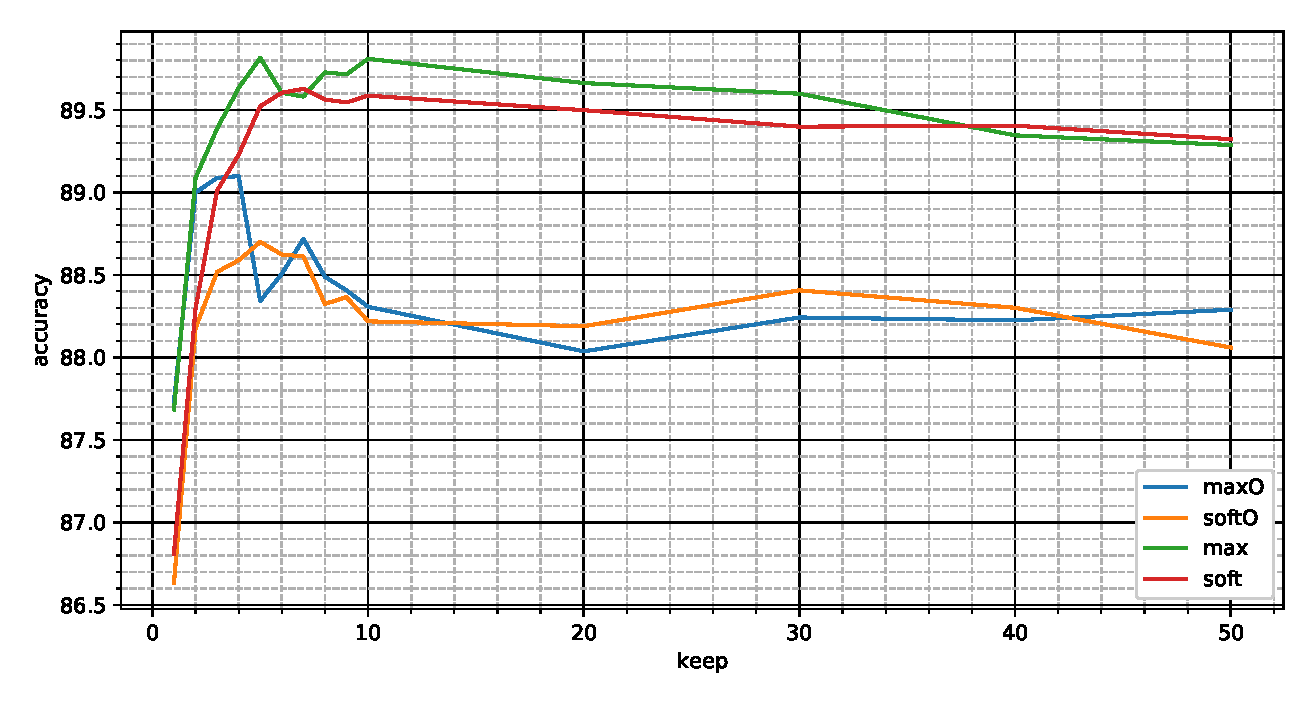
\includegraphics[width=\floatwidth]{img/plotSintex.eps}
  \caption{Training of a plain \ac{gru} model on a dataset created
    using \maxi{} and \softmaxi{} to keep the first $k$ words.}
  \label{fig:sintex}
\end{figure}
To quantify the effectiveness of the interpretability, we designed an
experiment where a dataset is created taking for each document the
first $k$ words selected by  
ordering the results of the aggregator $u_t$ in case of \maxi{}, and
$a_t(\vect{u};\theta^a)u_t$ in case of \softmaxi{}. In
\cref{fig:sintex}, 
we plot the accuracy obtained training a plain \ac{gru} model on the
cleaned datasets, for increasing values of $k$. Surprisingly,
even with few words the document is classified practically with
the same results as \gru{}. This can mean both that the
interpretation is working well distilling the document with its most
relevant terms, and that the information contained in our medical
texts is concentrated in few terms. The latter can also be the reason
why in \cref{tab:resultsSite,tab:resultsType} we do not observe a big
improvement in using deep learning methods respect to \acp{svm}.




%%% Local Variables:
%%% mode: latex
%%% TeX-master: "thesis"
%%% End:

% \include{.. add your chapters}
\chapter{Conclusions}
Since the cancer registration process is partially based on manual
revision, including also the interpretation of the free text in
pathological reports, significant delays in data production and
publication may occur. This weakens data relevance for the purpose of
assessing compliance with updated regional recommended integrated case
pathways, as well as for public health purposes. Improving automated
methods to generate a list of putative incident cases and to
automatically estimate process indicators is thus an opportunity to
perform an up-to-date evaluation of cancer-care quality. In
particular, machine learning techniques like the ones presented in
this paper could overcome the delay in cancer case definition by the
cancer registry and allow a powerful tool for timely indicators
computation. The implementation of this procedure could guarantee an
automated and validated instrument to monitor and evaluate diagnostic
and therapeutic pathways.

We analyzed the available data and created different models in order
to implement an automated classification system. We obtained very
encouraging results in classifying cancer cases based on the
interpretation of free text in the data-flow of pathology
reports. This suggests that machine learning methods can be usefully
leveraged in this context. Moreover, we demonstrated that unlabeled
data can 
be effectively used to construct useful word vectors and improve
classification accuracy. 

Our models also have the added value that they can be
utilized to retrieve records adjusting the precision-recall trade-off.

The use of administrative data sources that are up to date combined
with powerful machine learning techniques to automate text
classification is in the interest of the development of a standardized
surveillance system at Regional and National level. Stakeholders and
decision makers need timely and updated indicators to evaluate and
plan healthcare activities. The availability of timely indicators,
routinely and automatically produced, is technically possible. The
main novelty of this work is to show the power of machine learning
techniques applied to the classification of free text pathological
records. This was not yet been systematically implemented in other
Italian cancer registries. This provides a useful monitor tool for
cancer patients pathways, allowing to describe population’s general
health state and to establish public health goals.

The results of the interpretable models can be used to
assist the human classification process on simple records. It can be
used as
a form of text compression, highlighting the most important terms. On
more complex records it can be used to leverage the knowledge of the
model to gain insight on the decision process. To overcome the
limitations of the interpretable
model respect to the general model, in terms of
classification metrics, is it possible to combine the two variants. The
general model can be used to give a more
authoritative classification on the samples while at the same time,
the interpretable model can highlight the same samples.

We compared novel deep learning techniques and more classical models
to pathology records. In this specific context we did not obtain
significant improvements using novel deep learning approaches respect
to classic machine learning methods. Also, the attention methods
usually employed in text classification tasks do not have better
results respect to a more simple max pooling hard attention. Furthermore,
hierarchical models do not work better than plain models. Unsupervised
methods, in particular Word Vectors,
can be used successfully in the
domain of pathological text records. At the best of our knowledge, this
is the first large scale study of deep learning methods applied to
pathology records. Other studies where performed on smaller datasets
with records labeled with less classes.

Regarding the questions in \cref{sec:motivation}, Q1 is answered by
the fact that we implemented several different models to a large scale
dataset of cancer pathology reports. Q2 is answered by the fact that
we used attention models and \ac{bert} in our experiments. To answer
to Q3, from our experiments we have evidence that by using deep learning
methods we do not have a breakthrough compared to classic
\ac{ml} approaches in this specific domain. Regarding Q4, we observe
that hierarchical models are not beneficial in this context. Moreover,
we achieve a little improvement by using attention models, but in
this context a simple max aggregation is equally powerful to the
commonly used attention. About Q5 we observe a successful improvement
when we leverage the unlabeled data, thus we can conclude that
unsupervised techniques can be successfully used in this
context. Finally, in relation to Q6 we studied the potentialities of
interpretable models in the pathology records context.

%%% Local Variables:
%%% mode: latex
%%% TeX-master: "thesis"
%%% End:

\appendix{
  \chapter{Details of experiments}
\label{app:details}

Totally optional
\section{Setup of Experiment 1}
\section{Detailed results}
  % Optional, for details that cannot fit the main body
  \chapter{Publications}
\label{app:publications}

\subsection*{Journal papers}
\begin{enumerate}
\item \textbf{Stefano Martina}, Leonardo Ventura, Paolo Frasconi,
  ``Classification of cancer pathology reports: a large-scale comparative study'', \textit{Journal of Biomedical and Health Informatics}, in
  review.
  \textbf{Candidate's contributions}: prepared dataset, designed
  methods and experiments, designed algorithms
\end{enumerate}
\subsection*{Peer reviewed conference papers}
\subsection*{Workshop papers}
\subsection*{Papers under review}
\subsection*{Other}
(e.g. ArXiv preprints not yet submitted)


 % Mandatory
}
% End EDIT
%%%%%%%%%%%%%%%%%%%%%%%%%%%%%%%%%%%%%%%%%%%%%%%%%%%%%%%%%%%%%%%%%%%%%%%%%%%%%
\bibliographystyle{apalike}
\bibliography{Oncology,more,evenMore}
\end{document}

%%% Local Variables:
%%% mode: latex
%%% TeX-master: t
%%% End:
